\chapter{Literature Review}
\section{PDE-Based Failure Modeling}
Because material failure is an important part of many problems, there are several computational methods that attempt to simulate progressing material failure. 
Most of these methods start with the partial differential equations for conservation of momentum found in classical continuum mechanics, then extend those models to account for failure situations that are poorly modeled by the classical equations.

One of the most popular is the eXtended Finite Element Method (XFEM), an excellent overview of which can be found in~\cite{fries2010extended} by Fries and Belytschko.
Traditional finite elements use polynomial basis functions to describe unknown fields over an element.
As a result, fields such as displacement always vary continuously across an element; discontinuities within an element are poorly approximated even by high-order polynomials.
When they are allowed at all, discontinuities can only arise between elements, and are therefore very mesh-dependent; worse, to model a moving or evolving discontinuity requires continual remeshing around the advancing crack tip, adding greatly to the computational complexity of the problem.
The finite elements in an XFEM model are ``extended'' or enriched by adding basis functions that reflect the expected field behavior. 
In the case of crack growth, this extension comes in the form of discontinuous basis functions.
In 1982, Arnold~\cite{arnold1982interior} developed a mathematical basis for using discontinuous finite elements and an interior penalty method.
This method allows modeling problems with very high gradients (as at boundaries) and greatly reduces the importance of meshing and the need for remeshing.
While initially demonstrated for high-gradient heat and fluid flow problems, the method of adding discontinuities within an element had strong potential for failure problems resulting in discontinuous displacements.
Instead of remeshing along an expected crack path, a process that would require continual remeshing, the predicted direction of crack growth is used to choose discontinuous basis functions consistent with a crack along that path.

The use of discontinuous basis functions (such as \cref{fig:CrackEnrich}) to model crack progression through an element was first developed by Belytschko and Black in \cite{belytschko1999elastic} to model straight and gently curving cracks with less remeshing.
The discontinuous function in \cref{fig:CrackEnrich} will look familiar.
As the transverse displacement field around the tip of a Mode I crack,
\begin{equation}
\label{eq:modeIdisp}
v(x,y)=\frac{K_I}{2\mu}\sqrt{\frac{r}{2\mu}}\cos\left(\frac{\theta}{2}\right)\left[\kappa-1+2\sin^2\left(\frac{\theta}{2}\right)\right],
\end{equation}
\cref{eq:modeIdisp} and the other crack-tip displacement fields are a natural choice of basis functions.
Longer cracks would require remeshing, but at the root of the crack rather than the tip.
Root remeshing represents a major improvement over tip remeshing because it needs to be performed far less frequently.
Additionally, the path of the advancing crack can travel at any angle rather than following the angle of a mesh edge.
\begin{figure}[h]
  \centering
  \scalebox{.55}{%% Creator: Matplotlib, PGF backend
%%
%% To include the figure in your LaTeX document, write
%%   \input{<filename>.pgf}
%%
%% Make sure the required packages are loaded in your preamble
%%   \usepackage{pgf}
%%
%% Figures using additional raster images can only be included by \input if
%% they are in the same directory as the main LaTeX file. For loading figures
%% from other directories you can use the `import` package
%%   \usepackage{import}
%% and then include the figures with
%%   \import{<path to file>}{<filename>.pgf}
%%
%% Matplotlib used the following preamble
%%
\begingroup%
\makeatletter%
\begin{pgfpicture}%
\pgfpathrectangle{\pgfpointorigin}{\pgfqpoint{8.000000in}{6.000000in}}%
\pgfusepath{use as bounding box}%
\begin{pgfscope}%
\pgfsetbuttcap%
\pgfsetroundjoin%
\definecolor{currentfill}{rgb}{1.000000,1.000000,1.000000}%
\pgfsetfillcolor{currentfill}%
\pgfsetlinewidth{0.000000pt}%
\definecolor{currentstroke}{rgb}{1.000000,1.000000,1.000000}%
\pgfsetstrokecolor{currentstroke}%
\pgfsetdash{}{0pt}%
\pgfpathmoveto{\pgfqpoint{0.000000in}{0.000000in}}%
\pgfpathlineto{\pgfqpoint{8.000000in}{0.000000in}}%
\pgfpathlineto{\pgfqpoint{8.000000in}{6.000000in}}%
\pgfpathlineto{\pgfqpoint{0.000000in}{6.000000in}}%
\pgfpathclose%
\pgfusepath{fill}%
\end{pgfscope}%
\begin{pgfscope}%
\pgfsetbuttcap%
\pgfsetroundjoin%
\definecolor{currentfill}{rgb}{1.000000,1.000000,1.000000}%
\pgfsetfillcolor{currentfill}%
\pgfsetlinewidth{0.000000pt}%
\definecolor{currentstroke}{rgb}{0.000000,0.000000,0.000000}%
\pgfsetstrokecolor{currentstroke}%
\pgfsetstrokeopacity{0.000000}%
\pgfsetdash{}{0pt}%
\pgfpathmoveto{\pgfqpoint{0.180000in}{0.180000in}}%
\pgfpathlineto{\pgfqpoint{7.820000in}{0.180000in}}%
\pgfpathlineto{\pgfqpoint{7.820000in}{5.820000in}}%
\pgfpathlineto{\pgfqpoint{0.180000in}{5.820000in}}%
\pgfpathclose%
\pgfusepath{fill}%
\end{pgfscope}%
\begin{pgfscope}%
\pgfpathrectangle{\pgfqpoint{0.180000in}{0.180000in}}{\pgfqpoint{7.640000in}{5.640000in}} %
\pgfusepath{clip}%
\pgfsetbuttcap%
\pgfsetroundjoin%
\definecolor{currentfill}{rgb}{1.000000,0.012320,0.006160}%
\pgfsetfillcolor{currentfill}%
\pgfsetlinewidth{1.003750pt}%
\definecolor{currentstroke}{rgb}{0.000000,0.000000,0.000000}%
\pgfsetstrokecolor{currentstroke}%
\pgfsetdash{}{0pt}%
\pgfpathmoveto{\pgfqpoint{3.325396in}{4.934489in}}%
\pgfpathlineto{\pgfqpoint{3.413154in}{4.894367in}}%
\pgfpathlineto{\pgfqpoint{3.465281in}{4.924395in}}%
\pgfpathlineto{\pgfqpoint{3.377653in}{4.964206in}}%
\pgfpathlineto{\pgfqpoint{3.325396in}{4.934489in}}%
\pgfpathclose%
\pgfusepath{stroke,fill}%
\end{pgfscope}%
\begin{pgfscope}%
\pgfpathrectangle{\pgfqpoint{0.180000in}{0.180000in}}{\pgfqpoint{7.640000in}{5.640000in}} %
\pgfusepath{clip}%
\pgfsetbuttcap%
\pgfsetroundjoin%
\definecolor{currentfill}{rgb}{1.000000,0.049260,0.024637}%
\pgfsetfillcolor{currentfill}%
\pgfsetlinewidth{1.003750pt}%
\definecolor{currentstroke}{rgb}{0.000000,0.000000,0.000000}%
\pgfsetstrokecolor{currentstroke}%
\pgfsetdash{}{0pt}%
\pgfpathmoveto{\pgfqpoint{3.413154in}{4.894367in}}%
\pgfpathlineto{\pgfqpoint{3.501030in}{4.853787in}}%
\pgfpathlineto{\pgfqpoint{3.553026in}{4.884157in}}%
\pgfpathlineto{\pgfqpoint{3.465281in}{4.924395in}}%
\pgfpathlineto{\pgfqpoint{3.413154in}{4.894367in}}%
\pgfpathclose%
\pgfusepath{stroke,fill}%
\end{pgfscope}%
\begin{pgfscope}%
\pgfpathrectangle{\pgfqpoint{0.180000in}{0.180000in}}{\pgfqpoint{7.640000in}{5.640000in}} %
\pgfusepath{clip}%
\pgfsetbuttcap%
\pgfsetroundjoin%
\definecolor{currentfill}{rgb}{1.000000,0.086133,0.043107}%
\pgfsetfillcolor{currentfill}%
\pgfsetlinewidth{1.003750pt}%
\definecolor{currentstroke}{rgb}{0.000000,0.000000,0.000000}%
\pgfsetstrokecolor{currentstroke}%
\pgfsetdash{}{0pt}%
\pgfpathmoveto{\pgfqpoint{3.501030in}{4.853787in}}%
\pgfpathlineto{\pgfqpoint{3.589021in}{4.812748in}}%
\pgfpathlineto{\pgfqpoint{3.640886in}{4.843497in}}%
\pgfpathlineto{\pgfqpoint{3.553026in}{4.884157in}}%
\pgfpathlineto{\pgfqpoint{3.501030in}{4.853787in}}%
\pgfpathclose%
\pgfusepath{stroke,fill}%
\end{pgfscope}%
\begin{pgfscope}%
\pgfpathrectangle{\pgfqpoint{0.180000in}{0.180000in}}{\pgfqpoint{7.640000in}{5.640000in}} %
\pgfusepath{clip}%
\pgfsetbuttcap%
\pgfsetroundjoin%
\definecolor{currentfill}{rgb}{1.000000,0.012320,0.006160}%
\pgfsetfillcolor{currentfill}%
\pgfsetlinewidth{1.003750pt}%
\definecolor{currentstroke}{rgb}{0.000000,0.000000,0.000000}%
\pgfsetstrokecolor{currentstroke}%
\pgfsetdash{}{0pt}%
\pgfpathmoveto{\pgfqpoint{3.272945in}{4.904856in}}%
\pgfpathlineto{\pgfqpoint{3.360834in}{4.864436in}}%
\pgfpathlineto{\pgfqpoint{3.413154in}{4.894367in}}%
\pgfpathlineto{\pgfqpoint{3.325396in}{4.934489in}}%
\pgfpathlineto{\pgfqpoint{3.272945in}{4.904856in}}%
\pgfpathclose%
\pgfusepath{stroke,fill}%
\end{pgfscope}%
\begin{pgfscope}%
\pgfpathrectangle{\pgfqpoint{0.180000in}{0.180000in}}{\pgfqpoint{7.640000in}{5.640000in}} %
\pgfusepath{clip}%
\pgfsetbuttcap%
\pgfsetroundjoin%
\definecolor{currentfill}{rgb}{1.000000,0.135105,0.067708}%
\pgfsetfillcolor{currentfill}%
\pgfsetlinewidth{1.003750pt}%
\definecolor{currentstroke}{rgb}{0.000000,0.000000,0.000000}%
\pgfsetstrokecolor{currentstroke}%
\pgfsetdash{}{0pt}%
\pgfpathmoveto{\pgfqpoint{3.589021in}{4.812748in}}%
\pgfpathlineto{\pgfqpoint{3.677125in}{4.771256in}}%
\pgfpathlineto{\pgfqpoint{3.728860in}{4.802421in}}%
\pgfpathlineto{\pgfqpoint{3.640886in}{4.843497in}}%
\pgfpathlineto{\pgfqpoint{3.589021in}{4.812748in}}%
\pgfpathclose%
\pgfusepath{stroke,fill}%
\end{pgfscope}%
\begin{pgfscope}%
\pgfpathrectangle{\pgfqpoint{0.180000in}{0.180000in}}{\pgfqpoint{7.640000in}{5.640000in}} %
\pgfusepath{clip}%
\pgfsetbuttcap%
\pgfsetroundjoin%
\definecolor{currentfill}{rgb}{1.000000,0.049260,0.024637}%
\pgfsetfillcolor{currentfill}%
\pgfsetlinewidth{1.003750pt}%
\definecolor{currentstroke}{rgb}{0.000000,0.000000,0.000000}%
\pgfsetstrokecolor{currentstroke}%
\pgfsetdash{}{0pt}%
\pgfpathmoveto{\pgfqpoint{3.360834in}{4.864436in}}%
\pgfpathlineto{\pgfqpoint{3.448841in}{4.823524in}}%
\pgfpathlineto{\pgfqpoint{3.501030in}{4.853787in}}%
\pgfpathlineto{\pgfqpoint{3.413154in}{4.894367in}}%
\pgfpathlineto{\pgfqpoint{3.360834in}{4.864436in}}%
\pgfpathclose%
\pgfusepath{stroke,fill}%
\end{pgfscope}%
\begin{pgfscope}%
\pgfpathrectangle{\pgfqpoint{0.180000in}{0.180000in}}{\pgfqpoint{7.640000in}{5.640000in}} %
\pgfusepath{clip}%
\pgfsetbuttcap%
\pgfsetroundjoin%
\definecolor{currentfill}{rgb}{1.000000,0.171626,0.086133}%
\pgfsetfillcolor{currentfill}%
\pgfsetlinewidth{1.003750pt}%
\definecolor{currentstroke}{rgb}{0.000000,0.000000,0.000000}%
\pgfsetstrokecolor{currentstroke}%
\pgfsetdash{}{0pt}%
\pgfpathmoveto{\pgfqpoint{3.677125in}{4.771256in}}%
\pgfpathlineto{\pgfqpoint{3.765342in}{4.729321in}}%
\pgfpathlineto{\pgfqpoint{3.816945in}{4.760944in}}%
\pgfpathlineto{\pgfqpoint{3.728860in}{4.802421in}}%
\pgfpathlineto{\pgfqpoint{3.677125in}{4.771256in}}%
\pgfpathclose%
\pgfusepath{stroke,fill}%
\end{pgfscope}%
\begin{pgfscope}%
\pgfpathrectangle{\pgfqpoint{0.180000in}{0.180000in}}{\pgfqpoint{7.640000in}{5.640000in}} %
\pgfusepath{clip}%
\pgfsetbuttcap%
\pgfsetroundjoin%
\definecolor{currentfill}{rgb}{1.000000,0.086133,0.043107}%
\pgfsetfillcolor{currentfill}%
\pgfsetlinewidth{1.003750pt}%
\definecolor{currentstroke}{rgb}{0.000000,0.000000,0.000000}%
\pgfsetstrokecolor{currentstroke}%
\pgfsetdash{}{0pt}%
\pgfpathmoveto{\pgfqpoint{3.448841in}{4.823524in}}%
\pgfpathlineto{\pgfqpoint{3.536964in}{4.782118in}}%
\pgfpathlineto{\pgfqpoint{3.589021in}{4.812748in}}%
\pgfpathlineto{\pgfqpoint{3.501030in}{4.853787in}}%
\pgfpathlineto{\pgfqpoint{3.448841in}{4.823524in}}%
\pgfpathclose%
\pgfusepath{stroke,fill}%
\end{pgfscope}%
\begin{pgfscope}%
\pgfpathrectangle{\pgfqpoint{0.180000in}{0.180000in}}{\pgfqpoint{7.640000in}{5.640000in}} %
\pgfusepath{clip}%
\pgfsetbuttcap%
\pgfsetroundjoin%
\definecolor{currentfill}{rgb}{1.000000,0.207912,0.104528}%
\pgfsetfillcolor{currentfill}%
\pgfsetlinewidth{1.003750pt}%
\definecolor{currentstroke}{rgb}{0.000000,0.000000,0.000000}%
\pgfsetstrokecolor{currentstroke}%
\pgfsetdash{}{0pt}%
\pgfpathmoveto{\pgfqpoint{3.765342in}{4.729321in}}%
\pgfpathlineto{\pgfqpoint{3.853669in}{4.686958in}}%
\pgfpathlineto{\pgfqpoint{3.905142in}{4.719084in}}%
\pgfpathlineto{\pgfqpoint{3.816945in}{4.760944in}}%
\pgfpathlineto{\pgfqpoint{3.765342in}{4.729321in}}%
\pgfpathclose%
\pgfusepath{stroke,fill}%
\end{pgfscope}%
\begin{pgfscope}%
\pgfpathrectangle{\pgfqpoint{0.180000in}{0.180000in}}{\pgfqpoint{7.640000in}{5.640000in}} %
\pgfusepath{clip}%
\pgfsetbuttcap%
\pgfsetroundjoin%
\definecolor{currentfill}{rgb}{0.500000,0.000000,1.000000}%
\pgfsetfillcolor{currentfill}%
\pgfsetlinewidth{1.003750pt}%
\definecolor{currentstroke}{rgb}{0.000000,0.000000,0.000000}%
\pgfsetstrokecolor{currentstroke}%
\pgfsetdash{}{0pt}%
\pgfpathmoveto{\pgfqpoint{2.301263in}{2.494495in}}%
\pgfpathlineto{\pgfqpoint{2.387143in}{2.498179in}}%
\pgfpathlineto{\pgfqpoint{2.441399in}{2.531690in}}%
\pgfpathlineto{\pgfqpoint{2.355596in}{2.527978in}}%
\pgfpathlineto{\pgfqpoint{2.301263in}{2.494495in}}%
\pgfpathclose%
\pgfusepath{stroke,fill}%
\end{pgfscope}%
\begin{pgfscope}%
\pgfpathrectangle{\pgfqpoint{0.180000in}{0.180000in}}{\pgfqpoint{7.640000in}{5.640000in}} %
\pgfusepath{clip}%
\pgfsetbuttcap%
\pgfsetroundjoin%
\definecolor{currentfill}{rgb}{1.000000,0.012320,0.006160}%
\pgfsetfillcolor{currentfill}%
\pgfsetlinewidth{1.003750pt}%
\definecolor{currentstroke}{rgb}{0.000000,0.000000,0.000000}%
\pgfsetstrokecolor{currentstroke}%
\pgfsetdash{}{0pt}%
\pgfpathmoveto{\pgfqpoint{3.220296in}{4.875308in}}%
\pgfpathlineto{\pgfqpoint{3.308317in}{4.834603in}}%
\pgfpathlineto{\pgfqpoint{3.360834in}{4.864436in}}%
\pgfpathlineto{\pgfqpoint{3.272945in}{4.904856in}}%
\pgfpathlineto{\pgfqpoint{3.220296in}{4.875308in}}%
\pgfpathclose%
\pgfusepath{stroke,fill}%
\end{pgfscope}%
\begin{pgfscope}%
\pgfpathrectangle{\pgfqpoint{0.180000in}{0.180000in}}{\pgfqpoint{7.640000in}{5.640000in}} %
\pgfusepath{clip}%
\pgfsetbuttcap%
\pgfsetroundjoin%
\definecolor{currentfill}{rgb}{1.000000,0.135105,0.067708}%
\pgfsetfillcolor{currentfill}%
\pgfsetlinewidth{1.003750pt}%
\definecolor{currentstroke}{rgb}{0.000000,0.000000,0.000000}%
\pgfsetstrokecolor{currentstroke}%
\pgfsetdash{}{0pt}%
\pgfpathmoveto{\pgfqpoint{3.536964in}{4.782118in}}%
\pgfpathlineto{\pgfqpoint{3.625200in}{4.740218in}}%
\pgfpathlineto{\pgfqpoint{3.677125in}{4.771256in}}%
\pgfpathlineto{\pgfqpoint{3.589021in}{4.812748in}}%
\pgfpathlineto{\pgfqpoint{3.536964in}{4.782118in}}%
\pgfpathclose%
\pgfusepath{stroke,fill}%
\end{pgfscope}%
\begin{pgfscope}%
\pgfpathrectangle{\pgfqpoint{0.180000in}{0.180000in}}{\pgfqpoint{7.640000in}{5.640000in}} %
\pgfusepath{clip}%
\pgfsetbuttcap%
\pgfsetroundjoin%
\definecolor{currentfill}{rgb}{1.000000,0.255843,0.128999}%
\pgfsetfillcolor{currentfill}%
\pgfsetlinewidth{1.003750pt}%
\definecolor{currentstroke}{rgb}{0.000000,0.000000,0.000000}%
\pgfsetstrokecolor{currentstroke}%
\pgfsetdash{}{0pt}%
\pgfpathmoveto{\pgfqpoint{3.853669in}{4.686958in}}%
\pgfpathlineto{\pgfqpoint{3.942104in}{4.644193in}}%
\pgfpathlineto{\pgfqpoint{3.993447in}{4.676869in}}%
\pgfpathlineto{\pgfqpoint{3.905142in}{4.719084in}}%
\pgfpathlineto{\pgfqpoint{3.853669in}{4.686958in}}%
\pgfpathclose%
\pgfusepath{stroke,fill}%
\end{pgfscope}%
\begin{pgfscope}%
\pgfpathrectangle{\pgfqpoint{0.180000in}{0.180000in}}{\pgfqpoint{7.640000in}{5.640000in}} %
\pgfusepath{clip}%
\pgfsetbuttcap%
\pgfsetroundjoin%
\definecolor{currentfill}{rgb}{1.000000,0.049260,0.024637}%
\pgfsetfillcolor{currentfill}%
\pgfsetlinewidth{1.003750pt}%
\definecolor{currentstroke}{rgb}{0.000000,0.000000,0.000000}%
\pgfsetstrokecolor{currentstroke}%
\pgfsetdash{}{0pt}%
\pgfpathmoveto{\pgfqpoint{3.308317in}{4.834603in}}%
\pgfpathlineto{\pgfqpoint{3.396456in}{4.793375in}}%
\pgfpathlineto{\pgfqpoint{3.448841in}{4.823524in}}%
\pgfpathlineto{\pgfqpoint{3.360834in}{4.864436in}}%
\pgfpathlineto{\pgfqpoint{3.308317in}{4.834603in}}%
\pgfpathclose%
\pgfusepath{stroke,fill}%
\end{pgfscope}%
\begin{pgfscope}%
\pgfpathrectangle{\pgfqpoint{0.180000in}{0.180000in}}{\pgfqpoint{7.640000in}{5.640000in}} %
\pgfusepath{clip}%
\pgfsetbuttcap%
\pgfsetroundjoin%
\definecolor{currentfill}{rgb}{1.000000,0.171626,0.086133}%
\pgfsetfillcolor{currentfill}%
\pgfsetlinewidth{1.003750pt}%
\definecolor{currentstroke}{rgb}{0.000000,0.000000,0.000000}%
\pgfsetstrokecolor{currentstroke}%
\pgfsetdash{}{0pt}%
\pgfpathmoveto{\pgfqpoint{3.625200in}{4.740218in}}%
\pgfpathlineto{\pgfqpoint{3.713549in}{4.697830in}}%
\pgfpathlineto{\pgfqpoint{3.765342in}{4.729321in}}%
\pgfpathlineto{\pgfqpoint{3.677125in}{4.771256in}}%
\pgfpathlineto{\pgfqpoint{3.625200in}{4.740218in}}%
\pgfpathclose%
\pgfusepath{stroke,fill}%
\end{pgfscope}%
\begin{pgfscope}%
\pgfpathrectangle{\pgfqpoint{0.180000in}{0.180000in}}{\pgfqpoint{7.640000in}{5.640000in}} %
\pgfusepath{clip}%
\pgfsetbuttcap%
\pgfsetroundjoin%
\definecolor{currentfill}{rgb}{1.000000,0.291390,0.147302}%
\pgfsetfillcolor{currentfill}%
\pgfsetlinewidth{1.003750pt}%
\definecolor{currentstroke}{rgb}{0.000000,0.000000,0.000000}%
\pgfsetstrokecolor{currentstroke}%
\pgfsetdash{}{0pt}%
\pgfpathmoveto{\pgfqpoint{3.942104in}{4.644193in}}%
\pgfpathlineto{\pgfqpoint{4.030647in}{4.601059in}}%
\pgfpathlineto{\pgfqpoint{4.081860in}{4.634335in}}%
\pgfpathlineto{\pgfqpoint{3.993447in}{4.676869in}}%
\pgfpathlineto{\pgfqpoint{3.942104in}{4.644193in}}%
\pgfpathclose%
\pgfusepath{stroke,fill}%
\end{pgfscope}%
\begin{pgfscope}%
\pgfpathrectangle{\pgfqpoint{0.180000in}{0.180000in}}{\pgfqpoint{7.640000in}{5.640000in}} %
\pgfusepath{clip}%
\pgfsetbuttcap%
\pgfsetroundjoin%
\definecolor{currentfill}{rgb}{1.000000,0.338158,0.171626}%
\pgfsetfillcolor{currentfill}%
\pgfsetlinewidth{1.003750pt}%
\definecolor{currentstroke}{rgb}{0.000000,0.000000,0.000000}%
\pgfsetstrokecolor{currentstroke}%
\pgfsetdash{}{0pt}%
\pgfpathmoveto{\pgfqpoint{4.030647in}{4.601059in}}%
\pgfpathlineto{\pgfqpoint{4.119295in}{4.557599in}}%
\pgfpathlineto{\pgfqpoint{4.170380in}{4.591524in}}%
\pgfpathlineto{\pgfqpoint{4.081860in}{4.634335in}}%
\pgfpathlineto{\pgfqpoint{4.030647in}{4.601059in}}%
\pgfpathclose%
\pgfusepath{stroke,fill}%
\end{pgfscope}%
\begin{pgfscope}%
\pgfpathrectangle{\pgfqpoint{0.180000in}{0.180000in}}{\pgfqpoint{7.640000in}{5.640000in}} %
\pgfusepath{clip}%
\pgfsetbuttcap%
\pgfsetroundjoin%
\definecolor{currentfill}{rgb}{1.000000,0.086133,0.043107}%
\pgfsetfillcolor{currentfill}%
\pgfsetlinewidth{1.003750pt}%
\definecolor{currentstroke}{rgb}{0.000000,0.000000,0.000000}%
\pgfsetstrokecolor{currentstroke}%
\pgfsetdash{}{0pt}%
\pgfpathmoveto{\pgfqpoint{3.396456in}{4.793375in}}%
\pgfpathlineto{\pgfqpoint{3.484712in}{4.751615in}}%
\pgfpathlineto{\pgfqpoint{3.536964in}{4.782118in}}%
\pgfpathlineto{\pgfqpoint{3.448841in}{4.823524in}}%
\pgfpathlineto{\pgfqpoint{3.396456in}{4.793375in}}%
\pgfpathclose%
\pgfusepath{stroke,fill}%
\end{pgfscope}%
\begin{pgfscope}%
\pgfpathrectangle{\pgfqpoint{0.180000in}{0.180000in}}{\pgfqpoint{7.640000in}{5.640000in}} %
\pgfusepath{clip}%
\pgfsetbuttcap%
\pgfsetroundjoin%
\definecolor{currentfill}{rgb}{1.000000,0.219946,0.110653}%
\pgfsetfillcolor{currentfill}%
\pgfsetlinewidth{1.003750pt}%
\definecolor{currentstroke}{rgb}{0.000000,0.000000,0.000000}%
\pgfsetstrokecolor{currentstroke}%
\pgfsetdash{}{0pt}%
\pgfpathmoveto{\pgfqpoint{3.713549in}{4.697830in}}%
\pgfpathlineto{\pgfqpoint{3.802008in}{4.654966in}}%
\pgfpathlineto{\pgfqpoint{3.853669in}{4.686958in}}%
\pgfpathlineto{\pgfqpoint{3.765342in}{4.729321in}}%
\pgfpathlineto{\pgfqpoint{3.713549in}{4.697830in}}%
\pgfpathclose%
\pgfusepath{stroke,fill}%
\end{pgfscope}%
\begin{pgfscope}%
\pgfpathrectangle{\pgfqpoint{0.180000in}{0.180000in}}{\pgfqpoint{7.640000in}{5.640000in}} %
\pgfusepath{clip}%
\pgfsetbuttcap%
\pgfsetroundjoin%
\definecolor{currentfill}{rgb}{0.476471,0.036951,0.999829}%
\pgfsetfillcolor{currentfill}%
\pgfsetlinewidth{1.003750pt}%
\definecolor{currentstroke}{rgb}{0.000000,0.000000,0.000000}%
\pgfsetstrokecolor{currentstroke}%
\pgfsetdash{}{0pt}%
\pgfpathmoveto{\pgfqpoint{2.387143in}{2.498179in}}%
\pgfpathlineto{\pgfqpoint{2.473265in}{2.502513in}}%
\pgfpathlineto{\pgfqpoint{2.527444in}{2.536049in}}%
\pgfpathlineto{\pgfqpoint{2.441399in}{2.531690in}}%
\pgfpathlineto{\pgfqpoint{2.387143in}{2.498179in}}%
\pgfpathclose%
\pgfusepath{stroke,fill}%
\end{pgfscope}%
\begin{pgfscope}%
\pgfpathrectangle{\pgfqpoint{0.180000in}{0.180000in}}{\pgfqpoint{7.640000in}{5.640000in}} %
\pgfusepath{clip}%
\pgfsetbuttcap%
\pgfsetroundjoin%
\definecolor{currentfill}{rgb}{0.500000,0.000000,1.000000}%
\pgfsetfillcolor{currentfill}%
\pgfsetlinewidth{1.003750pt}%
\definecolor{currentstroke}{rgb}{0.000000,0.000000,0.000000}%
\pgfsetstrokecolor{currentstroke}%
\pgfsetdash{}{0pt}%
\pgfpathmoveto{\pgfqpoint{2.246721in}{2.461072in}}%
\pgfpathlineto{\pgfqpoint{2.332678in}{2.464742in}}%
\pgfpathlineto{\pgfqpoint{2.387143in}{2.498179in}}%
\pgfpathlineto{\pgfqpoint{2.301263in}{2.494495in}}%
\pgfpathlineto{\pgfqpoint{2.246721in}{2.461072in}}%
\pgfpathclose%
\pgfusepath{stroke,fill}%
\end{pgfscope}%
\begin{pgfscope}%
\pgfpathrectangle{\pgfqpoint{0.180000in}{0.180000in}}{\pgfqpoint{7.640000in}{5.640000in}} %
\pgfusepath{clip}%
\pgfsetbuttcap%
\pgfsetroundjoin%
\definecolor{currentfill}{rgb}{1.000000,0.384106,0.195845}%
\pgfsetfillcolor{currentfill}%
\pgfsetlinewidth{1.003750pt}%
\definecolor{currentstroke}{rgb}{0.000000,0.000000,0.000000}%
\pgfsetstrokecolor{currentstroke}%
\pgfsetdash{}{0pt}%
\pgfpathmoveto{\pgfqpoint{4.119295in}{4.557599in}}%
\pgfpathlineto{\pgfqpoint{4.208047in}{4.513870in}}%
\pgfpathlineto{\pgfqpoint{4.259006in}{4.548493in}}%
\pgfpathlineto{\pgfqpoint{4.170380in}{4.591524in}}%
\pgfpathlineto{\pgfqpoint{4.119295in}{4.557599in}}%
\pgfpathclose%
\pgfusepath{stroke,fill}%
\end{pgfscope}%
\begin{pgfscope}%
\pgfpathrectangle{\pgfqpoint{0.180000in}{0.180000in}}{\pgfqpoint{7.640000in}{5.640000in}} %
\pgfusepath{clip}%
\pgfsetbuttcap%
\pgfsetroundjoin%
\definecolor{currentfill}{rgb}{1.000000,0.012320,0.006160}%
\pgfsetfillcolor{currentfill}%
\pgfsetlinewidth{1.003750pt}%
\definecolor{currentstroke}{rgb}{0.000000,0.000000,0.000000}%
\pgfsetstrokecolor{currentstroke}%
\pgfsetdash{}{0pt}%
\pgfpathmoveto{\pgfqpoint{3.167449in}{4.845842in}}%
\pgfpathlineto{\pgfqpoint{3.255602in}{4.804871in}}%
\pgfpathlineto{\pgfqpoint{3.308317in}{4.834603in}}%
\pgfpathlineto{\pgfqpoint{3.220296in}{4.875308in}}%
\pgfpathlineto{\pgfqpoint{3.167449in}{4.845842in}}%
\pgfpathclose%
\pgfusepath{stroke,fill}%
\end{pgfscope}%
\begin{pgfscope}%
\pgfpathrectangle{\pgfqpoint{0.180000in}{0.180000in}}{\pgfqpoint{7.640000in}{5.640000in}} %
\pgfusepath{clip}%
\pgfsetbuttcap%
\pgfsetroundjoin%
\definecolor{currentfill}{rgb}{1.000000,0.255843,0.128999}%
\pgfsetfillcolor{currentfill}%
\pgfsetlinewidth{1.003750pt}%
\definecolor{currentstroke}{rgb}{0.000000,0.000000,0.000000}%
\pgfsetstrokecolor{currentstroke}%
\pgfsetdash{}{0pt}%
\pgfpathmoveto{\pgfqpoint{3.802008in}{4.654966in}}%
\pgfpathlineto{\pgfqpoint{3.890575in}{4.611648in}}%
\pgfpathlineto{\pgfqpoint{3.942104in}{4.644193in}}%
\pgfpathlineto{\pgfqpoint{3.853669in}{4.686958in}}%
\pgfpathlineto{\pgfqpoint{3.802008in}{4.654966in}}%
\pgfpathclose%
\pgfusepath{stroke,fill}%
\end{pgfscope}%
\begin{pgfscope}%
\pgfpathrectangle{\pgfqpoint{0.180000in}{0.180000in}}{\pgfqpoint{7.640000in}{5.640000in}} %
\pgfusepath{clip}%
\pgfsetbuttcap%
\pgfsetroundjoin%
\definecolor{currentfill}{rgb}{1.000000,0.135105,0.067708}%
\pgfsetfillcolor{currentfill}%
\pgfsetlinewidth{1.003750pt}%
\definecolor{currentstroke}{rgb}{0.000000,0.000000,0.000000}%
\pgfsetstrokecolor{currentstroke}%
\pgfsetdash{}{0pt}%
\pgfpathmoveto{\pgfqpoint{3.484712in}{4.751615in}}%
\pgfpathlineto{\pgfqpoint{3.573082in}{4.709318in}}%
\pgfpathlineto{\pgfqpoint{3.625200in}{4.740218in}}%
\pgfpathlineto{\pgfqpoint{3.536964in}{4.782118in}}%
\pgfpathlineto{\pgfqpoint{3.484712in}{4.751615in}}%
\pgfpathclose%
\pgfusepath{stroke,fill}%
\end{pgfscope}%
\begin{pgfscope}%
\pgfpathrectangle{\pgfqpoint{0.180000in}{0.180000in}}{\pgfqpoint{7.640000in}{5.640000in}} %
\pgfusepath{clip}%
\pgfsetbuttcap%
\pgfsetroundjoin%
\definecolor{currentfill}{rgb}{1.000000,0.417960,0.213933}%
\pgfsetfillcolor{currentfill}%
\pgfsetlinewidth{1.003750pt}%
\definecolor{currentstroke}{rgb}{0.000000,0.000000,0.000000}%
\pgfsetstrokecolor{currentstroke}%
\pgfsetdash{}{0pt}%
\pgfpathmoveto{\pgfqpoint{4.208047in}{4.513870in}}%
\pgfpathlineto{\pgfqpoint{4.296903in}{4.469939in}}%
\pgfpathlineto{\pgfqpoint{4.347737in}{4.505307in}}%
\pgfpathlineto{\pgfqpoint{4.259006in}{4.548493in}}%
\pgfpathlineto{\pgfqpoint{4.208047in}{4.513870in}}%
\pgfpathclose%
\pgfusepath{stroke,fill}%
\end{pgfscope}%
\begin{pgfscope}%
\pgfpathrectangle{\pgfqpoint{0.180000in}{0.180000in}}{\pgfqpoint{7.640000in}{5.640000in}} %
\pgfusepath{clip}%
\pgfsetbuttcap%
\pgfsetroundjoin%
\definecolor{currentfill}{rgb}{1.000000,0.303153,0.153392}%
\pgfsetfillcolor{currentfill}%
\pgfsetlinewidth{1.003750pt}%
\definecolor{currentstroke}{rgb}{0.000000,0.000000,0.000000}%
\pgfsetstrokecolor{currentstroke}%
\pgfsetdash{}{0pt}%
\pgfpathmoveto{\pgfqpoint{3.890575in}{4.611648in}}%
\pgfpathlineto{\pgfqpoint{3.979248in}{4.567906in}}%
\pgfpathlineto{\pgfqpoint{4.030647in}{4.601059in}}%
\pgfpathlineto{\pgfqpoint{3.942104in}{4.644193in}}%
\pgfpathlineto{\pgfqpoint{3.890575in}{4.611648in}}%
\pgfpathclose%
\pgfusepath{stroke,fill}%
\end{pgfscope}%
\begin{pgfscope}%
\pgfpathrectangle{\pgfqpoint{0.180000in}{0.180000in}}{\pgfqpoint{7.640000in}{5.640000in}} %
\pgfusepath{clip}%
\pgfsetbuttcap%
\pgfsetroundjoin%
\definecolor{currentfill}{rgb}{1.000000,0.049260,0.024637}%
\pgfsetfillcolor{currentfill}%
\pgfsetlinewidth{1.003750pt}%
\definecolor{currentstroke}{rgb}{0.000000,0.000000,0.000000}%
\pgfsetstrokecolor{currentstroke}%
\pgfsetdash{}{0pt}%
\pgfpathmoveto{\pgfqpoint{3.255602in}{4.804871in}}%
\pgfpathlineto{\pgfqpoint{3.343875in}{4.763342in}}%
\pgfpathlineto{\pgfqpoint{3.396456in}{4.793375in}}%
\pgfpathlineto{\pgfqpoint{3.308317in}{4.834603in}}%
\pgfpathlineto{\pgfqpoint{3.255602in}{4.804871in}}%
\pgfpathclose%
\pgfusepath{stroke,fill}%
\end{pgfscope}%
\begin{pgfscope}%
\pgfpathrectangle{\pgfqpoint{0.180000in}{0.180000in}}{\pgfqpoint{7.640000in}{5.640000in}} %
\pgfusepath{clip}%
\pgfsetbuttcap%
\pgfsetroundjoin%
\definecolor{currentfill}{rgb}{1.000000,0.171626,0.086133}%
\pgfsetfillcolor{currentfill}%
\pgfsetlinewidth{1.003750pt}%
\definecolor{currentstroke}{rgb}{0.000000,0.000000,0.000000}%
\pgfsetstrokecolor{currentstroke}%
\pgfsetdash{}{0pt}%
\pgfpathmoveto{\pgfqpoint{3.573082in}{4.709318in}}%
\pgfpathlineto{\pgfqpoint{3.661565in}{4.666487in}}%
\pgfpathlineto{\pgfqpoint{3.713549in}{4.697830in}}%
\pgfpathlineto{\pgfqpoint{3.625200in}{4.740218in}}%
\pgfpathlineto{\pgfqpoint{3.573082in}{4.709318in}}%
\pgfpathclose%
\pgfusepath{stroke,fill}%
\end{pgfscope}%
\begin{pgfscope}%
\pgfpathrectangle{\pgfqpoint{0.180000in}{0.180000in}}{\pgfqpoint{7.640000in}{5.640000in}} %
\pgfusepath{clip}%
\pgfsetbuttcap%
\pgfsetroundjoin%
\definecolor{currentfill}{rgb}{0.452941,0.073853,0.999317}%
\pgfsetfillcolor{currentfill}%
\pgfsetlinewidth{1.003750pt}%
\definecolor{currentstroke}{rgb}{0.000000,0.000000,0.000000}%
\pgfsetstrokecolor{currentstroke}%
\pgfsetdash{}{0pt}%
\pgfpathmoveto{\pgfqpoint{2.473265in}{2.502513in}}%
\pgfpathlineto{\pgfqpoint{2.559630in}{2.507556in}}%
\pgfpathlineto{\pgfqpoint{2.613732in}{2.541114in}}%
\pgfpathlineto{\pgfqpoint{2.527444in}{2.536049in}}%
\pgfpathlineto{\pgfqpoint{2.473265in}{2.502513in}}%
\pgfpathclose%
\pgfusepath{stroke,fill}%
\end{pgfscope}%
\begin{pgfscope}%
\pgfpathrectangle{\pgfqpoint{0.180000in}{0.180000in}}{\pgfqpoint{7.640000in}{5.640000in}} %
\pgfusepath{clip}%
\pgfsetbuttcap%
\pgfsetroundjoin%
\definecolor{currentfill}{rgb}{1.000000,0.462204,0.237935}%
\pgfsetfillcolor{currentfill}%
\pgfsetlinewidth{1.003750pt}%
\definecolor{currentstroke}{rgb}{0.000000,0.000000,0.000000}%
\pgfsetstrokecolor{currentstroke}%
\pgfsetdash{}{0pt}%
\pgfpathmoveto{\pgfqpoint{4.296903in}{4.469939in}}%
\pgfpathlineto{\pgfqpoint{4.385863in}{4.425888in}}%
\pgfpathlineto{\pgfqpoint{4.436574in}{4.462042in}}%
\pgfpathlineto{\pgfqpoint{4.347737in}{4.505307in}}%
\pgfpathlineto{\pgfqpoint{4.296903in}{4.469939in}}%
\pgfpathclose%
\pgfusepath{stroke,fill}%
\end{pgfscope}%
\begin{pgfscope}%
\pgfpathrectangle{\pgfqpoint{0.180000in}{0.180000in}}{\pgfqpoint{7.640000in}{5.640000in}} %
\pgfusepath{clip}%
\pgfsetbuttcap%
\pgfsetroundjoin%
\definecolor{currentfill}{rgb}{1.000000,0.349727,0.177691}%
\pgfsetfillcolor{currentfill}%
\pgfsetlinewidth{1.003750pt}%
\definecolor{currentstroke}{rgb}{0.000000,0.000000,0.000000}%
\pgfsetstrokecolor{currentstroke}%
\pgfsetdash{}{0pt}%
\pgfpathmoveto{\pgfqpoint{3.979248in}{4.567906in}}%
\pgfpathlineto{\pgfqpoint{4.068026in}{4.523781in}}%
\pgfpathlineto{\pgfqpoint{4.119295in}{4.557599in}}%
\pgfpathlineto{\pgfqpoint{4.030647in}{4.601059in}}%
\pgfpathlineto{\pgfqpoint{3.979248in}{4.567906in}}%
\pgfpathclose%
\pgfusepath{stroke,fill}%
\end{pgfscope}%
\begin{pgfscope}%
\pgfpathrectangle{\pgfqpoint{0.180000in}{0.180000in}}{\pgfqpoint{7.640000in}{5.640000in}} %
\pgfusepath{clip}%
\pgfsetbuttcap%
\pgfsetroundjoin%
\definecolor{currentfill}{rgb}{1.000000,0.219946,0.110653}%
\pgfsetfillcolor{currentfill}%
\pgfsetlinewidth{1.003750pt}%
\definecolor{currentstroke}{rgb}{0.000000,0.000000,0.000000}%
\pgfsetstrokecolor{currentstroke}%
\pgfsetdash{}{0pt}%
\pgfpathmoveto{\pgfqpoint{3.661565in}{4.666487in}}%
\pgfpathlineto{\pgfqpoint{3.750157in}{4.623128in}}%
\pgfpathlineto{\pgfqpoint{3.802008in}{4.654966in}}%
\pgfpathlineto{\pgfqpoint{3.713549in}{4.697830in}}%
\pgfpathlineto{\pgfqpoint{3.661565in}{4.666487in}}%
\pgfpathclose%
\pgfusepath{stroke,fill}%
\end{pgfscope}%
\begin{pgfscope}%
\pgfpathrectangle{\pgfqpoint{0.180000in}{0.180000in}}{\pgfqpoint{7.640000in}{5.640000in}} %
\pgfusepath{clip}%
\pgfsetbuttcap%
\pgfsetroundjoin%
\definecolor{currentfill}{rgb}{1.000000,0.098400,0.049260}%
\pgfsetfillcolor{currentfill}%
\pgfsetlinewidth{1.003750pt}%
\definecolor{currentstroke}{rgb}{0.000000,0.000000,0.000000}%
\pgfsetstrokecolor{currentstroke}%
\pgfsetdash{}{0pt}%
\pgfpathmoveto{\pgfqpoint{3.343875in}{4.763342in}}%
\pgfpathlineto{\pgfqpoint{3.432265in}{4.721245in}}%
\pgfpathlineto{\pgfqpoint{3.484712in}{4.751615in}}%
\pgfpathlineto{\pgfqpoint{3.396456in}{4.793375in}}%
\pgfpathlineto{\pgfqpoint{3.343875in}{4.763342in}}%
\pgfpathclose%
\pgfusepath{stroke,fill}%
\end{pgfscope}%
\begin{pgfscope}%
\pgfpathrectangle{\pgfqpoint{0.180000in}{0.180000in}}{\pgfqpoint{7.640000in}{5.640000in}} %
\pgfusepath{clip}%
\pgfsetbuttcap%
\pgfsetroundjoin%
\definecolor{currentfill}{rgb}{0.476471,0.036951,0.999829}%
\pgfsetfillcolor{currentfill}%
\pgfsetlinewidth{1.003750pt}%
\definecolor{currentstroke}{rgb}{0.000000,0.000000,0.000000}%
\pgfsetstrokecolor{currentstroke}%
\pgfsetdash{}{0pt}%
\pgfpathmoveto{\pgfqpoint{2.332678in}{2.464742in}}%
\pgfpathlineto{\pgfqpoint{2.418876in}{2.469066in}}%
\pgfpathlineto{\pgfqpoint{2.473265in}{2.502513in}}%
\pgfpathlineto{\pgfqpoint{2.387143in}{2.498179in}}%
\pgfpathlineto{\pgfqpoint{2.332678in}{2.464742in}}%
\pgfpathclose%
\pgfusepath{stroke,fill}%
\end{pgfscope}%
\begin{pgfscope}%
\pgfpathrectangle{\pgfqpoint{0.180000in}{0.180000in}}{\pgfqpoint{7.640000in}{5.640000in}} %
\pgfusepath{clip}%
\pgfsetbuttcap%
\pgfsetroundjoin%
\definecolor{currentfill}{rgb}{0.500000,0.000000,1.000000}%
\pgfsetfillcolor{currentfill}%
\pgfsetlinewidth{1.003750pt}%
\definecolor{currentstroke}{rgb}{0.000000,0.000000,0.000000}%
\pgfsetstrokecolor{currentstroke}%
\pgfsetdash{}{0pt}%
\pgfpathmoveto{\pgfqpoint{2.191969in}{2.427690in}}%
\pgfpathlineto{\pgfqpoint{2.278003in}{2.431355in}}%
\pgfpathlineto{\pgfqpoint{2.332678in}{2.464742in}}%
\pgfpathlineto{\pgfqpoint{2.246721in}{2.461072in}}%
\pgfpathlineto{\pgfqpoint{2.191969in}{2.427690in}}%
\pgfpathclose%
\pgfusepath{stroke,fill}%
\end{pgfscope}%
\begin{pgfscope}%
\pgfpathrectangle{\pgfqpoint{0.180000in}{0.180000in}}{\pgfqpoint{7.640000in}{5.640000in}} %
\pgfusepath{clip}%
\pgfsetbuttcap%
\pgfsetroundjoin%
\definecolor{currentfill}{rgb}{1.000000,0.505325,0.261793}%
\pgfsetfillcolor{currentfill}%
\pgfsetlinewidth{1.003750pt}%
\definecolor{currentstroke}{rgb}{0.000000,0.000000,0.000000}%
\pgfsetstrokecolor{currentstroke}%
\pgfsetdash{}{0pt}%
\pgfpathmoveto{\pgfqpoint{4.385863in}{4.425888in}}%
\pgfpathlineto{\pgfqpoint{4.474928in}{4.381811in}}%
\pgfpathlineto{\pgfqpoint{4.525518in}{4.418786in}}%
\pgfpathlineto{\pgfqpoint{4.436574in}{4.462042in}}%
\pgfpathlineto{\pgfqpoint{4.385863in}{4.425888in}}%
\pgfpathclose%
\pgfusepath{stroke,fill}%
\end{pgfscope}%
\begin{pgfscope}%
\pgfpathrectangle{\pgfqpoint{0.180000in}{0.180000in}}{\pgfqpoint{7.640000in}{5.640000in}} %
\pgfusepath{clip}%
\pgfsetbuttcap%
\pgfsetroundjoin%
\definecolor{currentfill}{rgb}{1.000000,0.384106,0.195845}%
\pgfsetfillcolor{currentfill}%
\pgfsetlinewidth{1.003750pt}%
\definecolor{currentstroke}{rgb}{0.000000,0.000000,0.000000}%
\pgfsetstrokecolor{currentstroke}%
\pgfsetdash{}{0pt}%
\pgfpathmoveto{\pgfqpoint{4.068026in}{4.523781in}}%
\pgfpathlineto{\pgfqpoint{4.156907in}{4.479330in}}%
\pgfpathlineto{\pgfqpoint{4.208047in}{4.513870in}}%
\pgfpathlineto{\pgfqpoint{4.119295in}{4.557599in}}%
\pgfpathlineto{\pgfqpoint{4.068026in}{4.523781in}}%
\pgfpathclose%
\pgfusepath{stroke,fill}%
\end{pgfscope}%
\begin{pgfscope}%
\pgfpathrectangle{\pgfqpoint{0.180000in}{0.180000in}}{\pgfqpoint{7.640000in}{5.640000in}} %
\pgfusepath{clip}%
\pgfsetbuttcap%
\pgfsetroundjoin%
\definecolor{currentfill}{rgb}{1.000000,0.267733,0.135105}%
\pgfsetfillcolor{currentfill}%
\pgfsetlinewidth{1.003750pt}%
\definecolor{currentstroke}{rgb}{0.000000,0.000000,0.000000}%
\pgfsetstrokecolor{currentstroke}%
\pgfsetdash{}{0pt}%
\pgfpathmoveto{\pgfqpoint{3.750157in}{4.623128in}}%
\pgfpathlineto{\pgfqpoint{3.838857in}{4.579257in}}%
\pgfpathlineto{\pgfqpoint{3.890575in}{4.611648in}}%
\pgfpathlineto{\pgfqpoint{3.802008in}{4.654966in}}%
\pgfpathlineto{\pgfqpoint{3.750157in}{4.623128in}}%
\pgfpathclose%
\pgfusepath{stroke,fill}%
\end{pgfscope}%
\begin{pgfscope}%
\pgfpathrectangle{\pgfqpoint{0.180000in}{0.180000in}}{\pgfqpoint{7.640000in}{5.640000in}} %
\pgfusepath{clip}%
\pgfsetbuttcap%
\pgfsetroundjoin%
\definecolor{currentfill}{rgb}{1.000000,0.012320,0.006160}%
\pgfsetfillcolor{currentfill}%
\pgfsetlinewidth{1.003750pt}%
\definecolor{currentstroke}{rgb}{0.000000,0.000000,0.000000}%
\pgfsetstrokecolor{currentstroke}%
\pgfsetdash{}{0pt}%
\pgfpathmoveto{\pgfqpoint{3.114401in}{4.816453in}}%
\pgfpathlineto{\pgfqpoint{3.202688in}{4.775235in}}%
\pgfpathlineto{\pgfqpoint{3.255602in}{4.804871in}}%
\pgfpathlineto{\pgfqpoint{3.167449in}{4.845842in}}%
\pgfpathlineto{\pgfqpoint{3.114401in}{4.816453in}}%
\pgfpathclose%
\pgfusepath{stroke,fill}%
\end{pgfscope}%
\begin{pgfscope}%
\pgfpathrectangle{\pgfqpoint{0.180000in}{0.180000in}}{\pgfqpoint{7.640000in}{5.640000in}} %
\pgfusepath{clip}%
\pgfsetbuttcap%
\pgfsetroundjoin%
\definecolor{currentfill}{rgb}{1.000000,0.135105,0.067708}%
\pgfsetfillcolor{currentfill}%
\pgfsetlinewidth{1.003750pt}%
\definecolor{currentstroke}{rgb}{0.000000,0.000000,0.000000}%
\pgfsetstrokecolor{currentstroke}%
\pgfsetdash{}{0pt}%
\pgfpathmoveto{\pgfqpoint{3.432265in}{4.721245in}}%
\pgfpathlineto{\pgfqpoint{3.520770in}{4.678567in}}%
\pgfpathlineto{\pgfqpoint{3.573082in}{4.709318in}}%
\pgfpathlineto{\pgfqpoint{3.484712in}{4.751615in}}%
\pgfpathlineto{\pgfqpoint{3.432265in}{4.721245in}}%
\pgfpathclose%
\pgfusepath{stroke,fill}%
\end{pgfscope}%
\begin{pgfscope}%
\pgfpathrectangle{\pgfqpoint{0.180000in}{0.180000in}}{\pgfqpoint{7.640000in}{5.640000in}} %
\pgfusepath{clip}%
\pgfsetbuttcap%
\pgfsetroundjoin%
\definecolor{currentfill}{rgb}{1.000000,0.536867,0.279583}%
\pgfsetfillcolor{currentfill}%
\pgfsetlinewidth{1.003750pt}%
\definecolor{currentstroke}{rgb}{0.000000,0.000000,0.000000}%
\pgfsetstrokecolor{currentstroke}%
\pgfsetdash{}{0pt}%
\pgfpathmoveto{\pgfqpoint{4.474928in}{4.381811in}}%
\pgfpathlineto{\pgfqpoint{4.564097in}{4.337816in}}%
\pgfpathlineto{\pgfqpoint{4.614570in}{4.375637in}}%
\pgfpathlineto{\pgfqpoint{4.525518in}{4.418786in}}%
\pgfpathlineto{\pgfqpoint{4.474928in}{4.381811in}}%
\pgfpathclose%
\pgfusepath{stroke,fill}%
\end{pgfscope}%
\begin{pgfscope}%
\pgfpathrectangle{\pgfqpoint{0.180000in}{0.180000in}}{\pgfqpoint{7.640000in}{5.640000in}} %
\pgfusepath{clip}%
\pgfsetbuttcap%
\pgfsetroundjoin%
\definecolor{currentfill}{rgb}{1.000000,0.429121,0.219946}%
\pgfsetfillcolor{currentfill}%
\pgfsetlinewidth{1.003750pt}%
\definecolor{currentstroke}{rgb}{0.000000,0.000000,0.000000}%
\pgfsetstrokecolor{currentstroke}%
\pgfsetdash{}{0pt}%
\pgfpathmoveto{\pgfqpoint{4.156907in}{4.479330in}}%
\pgfpathlineto{\pgfqpoint{4.245890in}{4.434622in}}%
\pgfpathlineto{\pgfqpoint{4.296903in}{4.469939in}}%
\pgfpathlineto{\pgfqpoint{4.208047in}{4.513870in}}%
\pgfpathlineto{\pgfqpoint{4.156907in}{4.479330in}}%
\pgfpathclose%
\pgfusepath{stroke,fill}%
\end{pgfscope}%
\begin{pgfscope}%
\pgfpathrectangle{\pgfqpoint{0.180000in}{0.180000in}}{\pgfqpoint{7.640000in}{5.640000in}} %
\pgfusepath{clip}%
\pgfsetbuttcap%
\pgfsetroundjoin%
\definecolor{currentfill}{rgb}{1.000000,0.303153,0.153392}%
\pgfsetfillcolor{currentfill}%
\pgfsetlinewidth{1.003750pt}%
\definecolor{currentstroke}{rgb}{0.000000,0.000000,0.000000}%
\pgfsetstrokecolor{currentstroke}%
\pgfsetdash{}{0pt}%
\pgfpathmoveto{\pgfqpoint{3.838857in}{4.579257in}}%
\pgfpathlineto{\pgfqpoint{3.927663in}{4.534902in}}%
\pgfpathlineto{\pgfqpoint{3.979248in}{4.567906in}}%
\pgfpathlineto{\pgfqpoint{3.890575in}{4.611648in}}%
\pgfpathlineto{\pgfqpoint{3.838857in}{4.579257in}}%
\pgfpathclose%
\pgfusepath{stroke,fill}%
\end{pgfscope}%
\begin{pgfscope}%
\pgfpathrectangle{\pgfqpoint{0.180000in}{0.180000in}}{\pgfqpoint{7.640000in}{5.640000in}} %
\pgfusepath{clip}%
\pgfsetbuttcap%
\pgfsetroundjoin%
\definecolor{currentfill}{rgb}{1.000000,0.183750,0.092268}%
\pgfsetfillcolor{currentfill}%
\pgfsetlinewidth{1.003750pt}%
\definecolor{currentstroke}{rgb}{0.000000,0.000000,0.000000}%
\pgfsetstrokecolor{currentstroke}%
\pgfsetdash{}{0pt}%
\pgfpathmoveto{\pgfqpoint{3.520770in}{4.678567in}}%
\pgfpathlineto{\pgfqpoint{3.609387in}{4.635306in}}%
\pgfpathlineto{\pgfqpoint{3.661565in}{4.666487in}}%
\pgfpathlineto{\pgfqpoint{3.573082in}{4.709318in}}%
\pgfpathlineto{\pgfqpoint{3.520770in}{4.678567in}}%
\pgfpathclose%
\pgfusepath{stroke,fill}%
\end{pgfscope}%
\begin{pgfscope}%
\pgfpathrectangle{\pgfqpoint{0.180000in}{0.180000in}}{\pgfqpoint{7.640000in}{5.640000in}} %
\pgfusepath{clip}%
\pgfsetbuttcap%
\pgfsetroundjoin%
\definecolor{currentfill}{rgb}{1.000000,0.049260,0.024637}%
\pgfsetfillcolor{currentfill}%
\pgfsetlinewidth{1.003750pt}%
\definecolor{currentstroke}{rgb}{0.000000,0.000000,0.000000}%
\pgfsetstrokecolor{currentstroke}%
\pgfsetdash{}{0pt}%
\pgfpathmoveto{\pgfqpoint{3.202688in}{4.775235in}}%
\pgfpathlineto{\pgfqpoint{3.291095in}{4.733427in}}%
\pgfpathlineto{\pgfqpoint{3.343875in}{4.763342in}}%
\pgfpathlineto{\pgfqpoint{3.255602in}{4.804871in}}%
\pgfpathlineto{\pgfqpoint{3.202688in}{4.775235in}}%
\pgfpathclose%
\pgfusepath{stroke,fill}%
\end{pgfscope}%
\begin{pgfscope}%
\pgfpathrectangle{\pgfqpoint{0.180000in}{0.180000in}}{\pgfqpoint{7.640000in}{5.640000in}} %
\pgfusepath{clip}%
\pgfsetbuttcap%
\pgfsetroundjoin%
\definecolor{currentfill}{rgb}{0.421569,0.122888,0.998103}%
\pgfsetfillcolor{currentfill}%
\pgfsetlinewidth{1.003750pt}%
\definecolor{currentstroke}{rgb}{0.000000,0.000000,0.000000}%
\pgfsetstrokecolor{currentstroke}%
\pgfsetdash{}{0pt}%
\pgfpathmoveto{\pgfqpoint{2.559630in}{2.507556in}}%
\pgfpathlineto{\pgfqpoint{2.646241in}{2.513377in}}%
\pgfpathlineto{\pgfqpoint{2.700267in}{2.546953in}}%
\pgfpathlineto{\pgfqpoint{2.613732in}{2.541114in}}%
\pgfpathlineto{\pgfqpoint{2.559630in}{2.507556in}}%
\pgfpathclose%
\pgfusepath{stroke,fill}%
\end{pgfscope}%
\begin{pgfscope}%
\pgfpathrectangle{\pgfqpoint{0.180000in}{0.180000in}}{\pgfqpoint{7.640000in}{5.640000in}} %
\pgfusepath{clip}%
\pgfsetbuttcap%
\pgfsetroundjoin%
\definecolor{currentfill}{rgb}{0.452941,0.073853,0.999317}%
\pgfsetfillcolor{currentfill}%
\pgfsetlinewidth{1.003750pt}%
\definecolor{currentstroke}{rgb}{0.000000,0.000000,0.000000}%
\pgfsetstrokecolor{currentstroke}%
\pgfsetdash{}{0pt}%
\pgfpathmoveto{\pgfqpoint{2.418876in}{2.469066in}}%
\pgfpathlineto{\pgfqpoint{2.505318in}{2.474105in}}%
\pgfpathlineto{\pgfqpoint{2.559630in}{2.507556in}}%
\pgfpathlineto{\pgfqpoint{2.473265in}{2.502513in}}%
\pgfpathlineto{\pgfqpoint{2.418876in}{2.469066in}}%
\pgfpathclose%
\pgfusepath{stroke,fill}%
\end{pgfscope}%
\begin{pgfscope}%
\pgfpathrectangle{\pgfqpoint{0.180000in}{0.180000in}}{\pgfqpoint{7.640000in}{5.640000in}} %
\pgfusepath{clip}%
\pgfsetbuttcap%
\pgfsetroundjoin%
\definecolor{currentfill}{rgb}{1.000000,0.473094,0.243914}%
\pgfsetfillcolor{currentfill}%
\pgfsetlinewidth{1.003750pt}%
\definecolor{currentstroke}{rgb}{0.000000,0.000000,0.000000}%
\pgfsetstrokecolor{currentstroke}%
\pgfsetdash{}{0pt}%
\pgfpathmoveto{\pgfqpoint{4.245890in}{4.434622in}}%
\pgfpathlineto{\pgfqpoint{4.334974in}{4.389743in}}%
\pgfpathlineto{\pgfqpoint{4.385863in}{4.425888in}}%
\pgfpathlineto{\pgfqpoint{4.296903in}{4.469939in}}%
\pgfpathlineto{\pgfqpoint{4.245890in}{4.434622in}}%
\pgfpathclose%
\pgfusepath{stroke,fill}%
\end{pgfscope}%
\begin{pgfscope}%
\pgfpathrectangle{\pgfqpoint{0.180000in}{0.180000in}}{\pgfqpoint{7.640000in}{5.640000in}} %
\pgfusepath{clip}%
\pgfsetbuttcap%
\pgfsetroundjoin%
\definecolor{currentfill}{rgb}{1.000000,0.577774,0.303153}%
\pgfsetfillcolor{currentfill}%
\pgfsetlinewidth{1.003750pt}%
\definecolor{currentstroke}{rgb}{0.000000,0.000000,0.000000}%
\pgfsetstrokecolor{currentstroke}%
\pgfsetdash{}{0pt}%
\pgfpathmoveto{\pgfqpoint{4.564097in}{4.337816in}}%
\pgfpathlineto{\pgfqpoint{4.653375in}{4.294020in}}%
\pgfpathlineto{\pgfqpoint{4.703731in}{4.332701in}}%
\pgfpathlineto{\pgfqpoint{4.614570in}{4.375637in}}%
\pgfpathlineto{\pgfqpoint{4.564097in}{4.337816in}}%
\pgfpathclose%
\pgfusepath{stroke,fill}%
\end{pgfscope}%
\begin{pgfscope}%
\pgfpathrectangle{\pgfqpoint{0.180000in}{0.180000in}}{\pgfqpoint{7.640000in}{5.640000in}} %
\pgfusepath{clip}%
\pgfsetbuttcap%
\pgfsetroundjoin%
\definecolor{currentfill}{rgb}{1.000000,0.349727,0.177691}%
\pgfsetfillcolor{currentfill}%
\pgfsetlinewidth{1.003750pt}%
\definecolor{currentstroke}{rgb}{0.000000,0.000000,0.000000}%
\pgfsetstrokecolor{currentstroke}%
\pgfsetdash{}{0pt}%
\pgfpathmoveto{\pgfqpoint{3.927663in}{4.534902in}}%
\pgfpathlineto{\pgfqpoint{4.016572in}{4.490100in}}%
\pgfpathlineto{\pgfqpoint{4.068026in}{4.523781in}}%
\pgfpathlineto{\pgfqpoint{3.979248in}{4.567906in}}%
\pgfpathlineto{\pgfqpoint{3.927663in}{4.534902in}}%
\pgfpathclose%
\pgfusepath{stroke,fill}%
\end{pgfscope}%
\begin{pgfscope}%
\pgfpathrectangle{\pgfqpoint{0.180000in}{0.180000in}}{\pgfqpoint{7.640000in}{5.640000in}} %
\pgfusepath{clip}%
\pgfsetbuttcap%
\pgfsetroundjoin%
\definecolor{currentfill}{rgb}{1.000000,0.219946,0.110653}%
\pgfsetfillcolor{currentfill}%
\pgfsetlinewidth{1.003750pt}%
\definecolor{currentstroke}{rgb}{0.000000,0.000000,0.000000}%
\pgfsetstrokecolor{currentstroke}%
\pgfsetdash{}{0pt}%
\pgfpathmoveto{\pgfqpoint{3.609387in}{4.635306in}}%
\pgfpathlineto{\pgfqpoint{3.698114in}{4.591462in}}%
\pgfpathlineto{\pgfqpoint{3.750157in}{4.623128in}}%
\pgfpathlineto{\pgfqpoint{3.661565in}{4.666487in}}%
\pgfpathlineto{\pgfqpoint{3.609387in}{4.635306in}}%
\pgfpathclose%
\pgfusepath{stroke,fill}%
\end{pgfscope}%
\begin{pgfscope}%
\pgfpathrectangle{\pgfqpoint{0.180000in}{0.180000in}}{\pgfqpoint{7.640000in}{5.640000in}} %
\pgfusepath{clip}%
\pgfsetbuttcap%
\pgfsetroundjoin%
\definecolor{currentfill}{rgb}{1.000000,0.098400,0.049260}%
\pgfsetfillcolor{currentfill}%
\pgfsetlinewidth{1.003750pt}%
\definecolor{currentstroke}{rgb}{0.000000,0.000000,0.000000}%
\pgfsetstrokecolor{currentstroke}%
\pgfsetdash{}{0pt}%
\pgfpathmoveto{\pgfqpoint{3.291095in}{4.733427in}}%
\pgfpathlineto{\pgfqpoint{3.379620in}{4.691012in}}%
\pgfpathlineto{\pgfqpoint{3.432265in}{4.721245in}}%
\pgfpathlineto{\pgfqpoint{3.343875in}{4.763342in}}%
\pgfpathlineto{\pgfqpoint{3.291095in}{4.733427in}}%
\pgfpathclose%
\pgfusepath{stroke,fill}%
\end{pgfscope}%
\begin{pgfscope}%
\pgfpathrectangle{\pgfqpoint{0.180000in}{0.180000in}}{\pgfqpoint{7.640000in}{5.640000in}} %
\pgfusepath{clip}%
\pgfsetbuttcap%
\pgfsetroundjoin%
\definecolor{currentfill}{rgb}{0.476471,0.036951,0.999829}%
\pgfsetfillcolor{currentfill}%
\pgfsetlinewidth{1.003750pt}%
\definecolor{currentstroke}{rgb}{0.000000,0.000000,0.000000}%
\pgfsetstrokecolor{currentstroke}%
\pgfsetdash{}{0pt}%
\pgfpathmoveto{\pgfqpoint{2.278003in}{2.431355in}}%
\pgfpathlineto{\pgfqpoint{2.364277in}{2.435681in}}%
\pgfpathlineto{\pgfqpoint{2.418876in}{2.469066in}}%
\pgfpathlineto{\pgfqpoint{2.332678in}{2.464742in}}%
\pgfpathlineto{\pgfqpoint{2.278003in}{2.431355in}}%
\pgfpathclose%
\pgfusepath{stroke,fill}%
\end{pgfscope}%
\begin{pgfscope}%
\pgfpathrectangle{\pgfqpoint{0.180000in}{0.180000in}}{\pgfqpoint{7.640000in}{5.640000in}} %
\pgfusepath{clip}%
\pgfsetbuttcap%
\pgfsetroundjoin%
\definecolor{currentfill}{rgb}{1.000000,0.515918,0.267733}%
\pgfsetfillcolor{currentfill}%
\pgfsetlinewidth{1.003750pt}%
\definecolor{currentstroke}{rgb}{0.000000,0.000000,0.000000}%
\pgfsetstrokecolor{currentstroke}%
\pgfsetdash{}{0pt}%
\pgfpathmoveto{\pgfqpoint{4.334974in}{4.389743in}}%
\pgfpathlineto{\pgfqpoint{4.424161in}{4.344796in}}%
\pgfpathlineto{\pgfqpoint{4.474928in}{4.381811in}}%
\pgfpathlineto{\pgfqpoint{4.385863in}{4.425888in}}%
\pgfpathlineto{\pgfqpoint{4.334974in}{4.389743in}}%
\pgfpathclose%
\pgfusepath{stroke,fill}%
\end{pgfscope}%
\begin{pgfscope}%
\pgfpathrectangle{\pgfqpoint{0.180000in}{0.180000in}}{\pgfqpoint{7.640000in}{5.640000in}} %
\pgfusepath{clip}%
\pgfsetbuttcap%
\pgfsetroundjoin%
\definecolor{currentfill}{rgb}{1.000000,0.617278,0.326539}%
\pgfsetfillcolor{currentfill}%
\pgfsetlinewidth{1.003750pt}%
\definecolor{currentstroke}{rgb}{0.000000,0.000000,0.000000}%
\pgfsetstrokecolor{currentstroke}%
\pgfsetdash{}{0pt}%
\pgfpathmoveto{\pgfqpoint{4.653375in}{4.294020in}}%
\pgfpathlineto{\pgfqpoint{4.742762in}{4.250550in}}%
\pgfpathlineto{\pgfqpoint{4.793006in}{4.290088in}}%
\pgfpathlineto{\pgfqpoint{4.703731in}{4.332701in}}%
\pgfpathlineto{\pgfqpoint{4.653375in}{4.294020in}}%
\pgfpathclose%
\pgfusepath{stroke,fill}%
\end{pgfscope}%
\begin{pgfscope}%
\pgfpathrectangle{\pgfqpoint{0.180000in}{0.180000in}}{\pgfqpoint{7.640000in}{5.640000in}} %
\pgfusepath{clip}%
\pgfsetbuttcap%
\pgfsetroundjoin%
\definecolor{currentfill}{rgb}{0.500000,0.000000,1.000000}%
\pgfsetfillcolor{currentfill}%
\pgfsetlinewidth{1.003750pt}%
\definecolor{currentstroke}{rgb}{0.000000,0.000000,0.000000}%
\pgfsetstrokecolor{currentstroke}%
\pgfsetdash{}{0pt}%
\pgfpathmoveto{\pgfqpoint{2.137006in}{2.394323in}}%
\pgfpathlineto{\pgfqpoint{2.223116in}{2.397989in}}%
\pgfpathlineto{\pgfqpoint{2.278003in}{2.431355in}}%
\pgfpathlineto{\pgfqpoint{2.191969in}{2.427690in}}%
\pgfpathlineto{\pgfqpoint{2.137006in}{2.394323in}}%
\pgfpathclose%
\pgfusepath{stroke,fill}%
\end{pgfscope}%
\begin{pgfscope}%
\pgfpathrectangle{\pgfqpoint{0.180000in}{0.180000in}}{\pgfqpoint{7.640000in}{5.640000in}} %
\pgfusepath{clip}%
\pgfsetbuttcap%
\pgfsetroundjoin%
\definecolor{currentfill}{rgb}{1.000000,0.395451,0.201882}%
\pgfsetfillcolor{currentfill}%
\pgfsetlinewidth{1.003750pt}%
\definecolor{currentstroke}{rgb}{0.000000,0.000000,0.000000}%
\pgfsetstrokecolor{currentstroke}%
\pgfsetdash{}{0pt}%
\pgfpathmoveto{\pgfqpoint{4.016572in}{4.490100in}}%
\pgfpathlineto{\pgfqpoint{4.105584in}{4.444905in}}%
\pgfpathlineto{\pgfqpoint{4.156907in}{4.479330in}}%
\pgfpathlineto{\pgfqpoint{4.068026in}{4.523781in}}%
\pgfpathlineto{\pgfqpoint{4.016572in}{4.490100in}}%
\pgfpathclose%
\pgfusepath{stroke,fill}%
\end{pgfscope}%
\begin{pgfscope}%
\pgfpathrectangle{\pgfqpoint{0.180000in}{0.180000in}}{\pgfqpoint{7.640000in}{5.640000in}} %
\pgfusepath{clip}%
\pgfsetbuttcap%
\pgfsetroundjoin%
\definecolor{currentfill}{rgb}{1.000000,0.267733,0.135105}%
\pgfsetfillcolor{currentfill}%
\pgfsetlinewidth{1.003750pt}%
\definecolor{currentstroke}{rgb}{0.000000,0.000000,0.000000}%
\pgfsetstrokecolor{currentstroke}%
\pgfsetdash{}{0pt}%
\pgfpathmoveto{\pgfqpoint{3.698114in}{4.591462in}}%
\pgfpathlineto{\pgfqpoint{3.786949in}{4.547045in}}%
\pgfpathlineto{\pgfqpoint{3.838857in}{4.579257in}}%
\pgfpathlineto{\pgfqpoint{3.750157in}{4.623128in}}%
\pgfpathlineto{\pgfqpoint{3.698114in}{4.591462in}}%
\pgfpathclose%
\pgfusepath{stroke,fill}%
\end{pgfscope}%
\begin{pgfscope}%
\pgfpathrectangle{\pgfqpoint{0.180000in}{0.180000in}}{\pgfqpoint{7.640000in}{5.640000in}} %
\pgfusepath{clip}%
\pgfsetbuttcap%
\pgfsetroundjoin%
\definecolor{currentfill}{rgb}{1.000000,0.135105,0.067708}%
\pgfsetfillcolor{currentfill}%
\pgfsetlinewidth{1.003750pt}%
\definecolor{currentstroke}{rgb}{0.000000,0.000000,0.000000}%
\pgfsetstrokecolor{currentstroke}%
\pgfsetdash{}{0pt}%
\pgfpathmoveto{\pgfqpoint{3.379620in}{4.691012in}}%
\pgfpathlineto{\pgfqpoint{3.468260in}{4.647973in}}%
\pgfpathlineto{\pgfqpoint{3.520770in}{4.678567in}}%
\pgfpathlineto{\pgfqpoint{3.432265in}{4.721245in}}%
\pgfpathlineto{\pgfqpoint{3.379620in}{4.691012in}}%
\pgfpathclose%
\pgfusepath{stroke,fill}%
\end{pgfscope}%
\begin{pgfscope}%
\pgfpathrectangle{\pgfqpoint{0.180000in}{0.180000in}}{\pgfqpoint{7.640000in}{5.640000in}} %
\pgfusepath{clip}%
\pgfsetbuttcap%
\pgfsetroundjoin%
\definecolor{currentfill}{rgb}{1.000000,0.012320,0.006160}%
\pgfsetfillcolor{currentfill}%
\pgfsetlinewidth{1.003750pt}%
\definecolor{currentstroke}{rgb}{0.000000,0.000000,0.000000}%
\pgfsetstrokecolor{currentstroke}%
\pgfsetdash{}{0pt}%
\pgfpathmoveto{\pgfqpoint{3.061152in}{4.787134in}}%
\pgfpathlineto{\pgfqpoint{3.149573in}{4.745689in}}%
\pgfpathlineto{\pgfqpoint{3.202688in}{4.775235in}}%
\pgfpathlineto{\pgfqpoint{3.114401in}{4.816453in}}%
\pgfpathlineto{\pgfqpoint{3.061152in}{4.787134in}}%
\pgfpathclose%
\pgfusepath{stroke,fill}%
\end{pgfscope}%
\begin{pgfscope}%
\pgfpathrectangle{\pgfqpoint{0.180000in}{0.180000in}}{\pgfqpoint{7.640000in}{5.640000in}} %
\pgfusepath{clip}%
\pgfsetbuttcap%
\pgfsetroundjoin%
\definecolor{currentfill}{rgb}{1.000000,0.547220,0.285492}%
\pgfsetfillcolor{currentfill}%
\pgfsetlinewidth{1.003750pt}%
\definecolor{currentstroke}{rgb}{0.000000,0.000000,0.000000}%
\pgfsetstrokecolor{currentstroke}%
\pgfsetdash{}{0pt}%
\pgfpathmoveto{\pgfqpoint{4.424161in}{4.344796in}}%
\pgfpathlineto{\pgfqpoint{4.513451in}{4.299897in}}%
\pgfpathlineto{\pgfqpoint{4.564097in}{4.337816in}}%
\pgfpathlineto{\pgfqpoint{4.474928in}{4.381811in}}%
\pgfpathlineto{\pgfqpoint{4.424161in}{4.344796in}}%
\pgfpathclose%
\pgfusepath{stroke,fill}%
\end{pgfscope}%
\begin{pgfscope}%
\pgfpathrectangle{\pgfqpoint{0.180000in}{0.180000in}}{\pgfqpoint{7.640000in}{5.640000in}} %
\pgfusepath{clip}%
\pgfsetbuttcap%
\pgfsetroundjoin%
\definecolor{currentfill}{rgb}{0.390196,0.171626,0.996284}%
\pgfsetfillcolor{currentfill}%
\pgfsetlinewidth{1.003750pt}%
\definecolor{currentstroke}{rgb}{0.000000,0.000000,0.000000}%
\pgfsetstrokecolor{currentstroke}%
\pgfsetdash{}{0pt}%
\pgfpathmoveto{\pgfqpoint{2.646241in}{2.513377in}}%
\pgfpathlineto{\pgfqpoint{2.733102in}{2.520055in}}%
\pgfpathlineto{\pgfqpoint{2.787051in}{2.553643in}}%
\pgfpathlineto{\pgfqpoint{2.700267in}{2.546953in}}%
\pgfpathlineto{\pgfqpoint{2.646241in}{2.513377in}}%
\pgfpathclose%
\pgfusepath{stroke,fill}%
\end{pgfscope}%
\begin{pgfscope}%
\pgfpathrectangle{\pgfqpoint{0.180000in}{0.180000in}}{\pgfqpoint{7.640000in}{5.640000in}} %
\pgfusepath{clip}%
\pgfsetbuttcap%
\pgfsetroundjoin%
\definecolor{currentfill}{rgb}{1.000000,0.440216,0.225951}%
\pgfsetfillcolor{currentfill}%
\pgfsetlinewidth{1.003750pt}%
\definecolor{currentstroke}{rgb}{0.000000,0.000000,0.000000}%
\pgfsetstrokecolor{currentstroke}%
\pgfsetdash{}{0pt}%
\pgfpathmoveto{\pgfqpoint{4.105584in}{4.444905in}}%
\pgfpathlineto{\pgfqpoint{4.194695in}{4.399389in}}%
\pgfpathlineto{\pgfqpoint{4.245890in}{4.434622in}}%
\pgfpathlineto{\pgfqpoint{4.156907in}{4.479330in}}%
\pgfpathlineto{\pgfqpoint{4.105584in}{4.444905in}}%
\pgfpathclose%
\pgfusepath{stroke,fill}%
\end{pgfscope}%
\begin{pgfscope}%
\pgfpathrectangle{\pgfqpoint{0.180000in}{0.180000in}}{\pgfqpoint{7.640000in}{5.640000in}} %
\pgfusepath{clip}%
\pgfsetbuttcap%
\pgfsetroundjoin%
\definecolor{currentfill}{rgb}{1.000000,0.645928,0.343949}%
\pgfsetfillcolor{currentfill}%
\pgfsetlinewidth{1.003750pt}%
\definecolor{currentstroke}{rgb}{0.000000,0.000000,0.000000}%
\pgfsetstrokecolor{currentstroke}%
\pgfsetdash{}{0pt}%
\pgfpathmoveto{\pgfqpoint{4.742762in}{4.250550in}}%
\pgfpathlineto{\pgfqpoint{4.832264in}{4.207536in}}%
\pgfpathlineto{\pgfqpoint{4.882397in}{4.247913in}}%
\pgfpathlineto{\pgfqpoint{4.793006in}{4.290088in}}%
\pgfpathlineto{\pgfqpoint{4.742762in}{4.250550in}}%
\pgfpathclose%
\pgfusepath{stroke,fill}%
\end{pgfscope}%
\begin{pgfscope}%
\pgfpathrectangle{\pgfqpoint{0.180000in}{0.180000in}}{\pgfqpoint{7.640000in}{5.640000in}} %
\pgfusepath{clip}%
\pgfsetbuttcap%
\pgfsetroundjoin%
\definecolor{currentfill}{rgb}{1.000000,0.314870,0.159476}%
\pgfsetfillcolor{currentfill}%
\pgfsetlinewidth{1.003750pt}%
\definecolor{currentstroke}{rgb}{0.000000,0.000000,0.000000}%
\pgfsetstrokecolor{currentstroke}%
\pgfsetdash{}{0pt}%
\pgfpathmoveto{\pgfqpoint{3.786949in}{4.547045in}}%
\pgfpathlineto{\pgfqpoint{3.875889in}{4.502075in}}%
\pgfpathlineto{\pgfqpoint{3.927663in}{4.534902in}}%
\pgfpathlineto{\pgfqpoint{3.838857in}{4.579257in}}%
\pgfpathlineto{\pgfqpoint{3.786949in}{4.547045in}}%
\pgfpathclose%
\pgfusepath{stroke,fill}%
\end{pgfscope}%
\begin{pgfscope}%
\pgfpathrectangle{\pgfqpoint{0.180000in}{0.180000in}}{\pgfqpoint{7.640000in}{5.640000in}} %
\pgfusepath{clip}%
\pgfsetbuttcap%
\pgfsetroundjoin%
\definecolor{currentfill}{rgb}{1.000000,0.183750,0.092268}%
\pgfsetfillcolor{currentfill}%
\pgfsetlinewidth{1.003750pt}%
\definecolor{currentstroke}{rgb}{0.000000,0.000000,0.000000}%
\pgfsetstrokecolor{currentstroke}%
\pgfsetdash{}{0pt}%
\pgfpathmoveto{\pgfqpoint{3.468260in}{4.647973in}}%
\pgfpathlineto{\pgfqpoint{3.557013in}{4.604300in}}%
\pgfpathlineto{\pgfqpoint{3.609387in}{4.635306in}}%
\pgfpathlineto{\pgfqpoint{3.520770in}{4.678567in}}%
\pgfpathlineto{\pgfqpoint{3.468260in}{4.647973in}}%
\pgfpathclose%
\pgfusepath{stroke,fill}%
\end{pgfscope}%
\begin{pgfscope}%
\pgfpathrectangle{\pgfqpoint{0.180000in}{0.180000in}}{\pgfqpoint{7.640000in}{5.640000in}} %
\pgfusepath{clip}%
\pgfsetbuttcap%
\pgfsetroundjoin%
\definecolor{currentfill}{rgb}{1.000000,0.049260,0.024637}%
\pgfsetfillcolor{currentfill}%
\pgfsetlinewidth{1.003750pt}%
\definecolor{currentstroke}{rgb}{0.000000,0.000000,0.000000}%
\pgfsetstrokecolor{currentstroke}%
\pgfsetdash{}{0pt}%
\pgfpathmoveto{\pgfqpoint{3.149573in}{4.745689in}}%
\pgfpathlineto{\pgfqpoint{3.238115in}{4.703624in}}%
\pgfpathlineto{\pgfqpoint{3.291095in}{4.733427in}}%
\pgfpathlineto{\pgfqpoint{3.202688in}{4.775235in}}%
\pgfpathlineto{\pgfqpoint{3.149573in}{4.745689in}}%
\pgfpathclose%
\pgfusepath{stroke,fill}%
\end{pgfscope}%
\begin{pgfscope}%
\pgfpathrectangle{\pgfqpoint{0.180000in}{0.180000in}}{\pgfqpoint{7.640000in}{5.640000in}} %
\pgfusepath{clip}%
\pgfsetbuttcap%
\pgfsetroundjoin%
\definecolor{currentfill}{rgb}{0.421569,0.122888,0.998103}%
\pgfsetfillcolor{currentfill}%
\pgfsetlinewidth{1.003750pt}%
\definecolor{currentstroke}{rgb}{0.000000,0.000000,0.000000}%
\pgfsetstrokecolor{currentstroke}%
\pgfsetdash{}{0pt}%
\pgfpathmoveto{\pgfqpoint{2.505318in}{2.474105in}}%
\pgfpathlineto{\pgfqpoint{2.592005in}{2.479928in}}%
\pgfpathlineto{\pgfqpoint{2.646241in}{2.513377in}}%
\pgfpathlineto{\pgfqpoint{2.559630in}{2.507556in}}%
\pgfpathlineto{\pgfqpoint{2.505318in}{2.474105in}}%
\pgfpathclose%
\pgfusepath{stroke,fill}%
\end{pgfscope}%
\begin{pgfscope}%
\pgfpathrectangle{\pgfqpoint{0.180000in}{0.180000in}}{\pgfqpoint{7.640000in}{5.640000in}} %
\pgfusepath{clip}%
\pgfsetbuttcap%
\pgfsetroundjoin%
\definecolor{currentfill}{rgb}{1.000000,0.587785,0.309017}%
\pgfsetfillcolor{currentfill}%
\pgfsetlinewidth{1.003750pt}%
\definecolor{currentstroke}{rgb}{0.000000,0.000000,0.000000}%
\pgfsetstrokecolor{currentstroke}%
\pgfsetdash{}{0pt}%
\pgfpathmoveto{\pgfqpoint{4.513451in}{4.299897in}}%
\pgfpathlineto{\pgfqpoint{4.602845in}{4.255179in}}%
\pgfpathlineto{\pgfqpoint{4.653375in}{4.294020in}}%
\pgfpathlineto{\pgfqpoint{4.564097in}{4.337816in}}%
\pgfpathlineto{\pgfqpoint{4.513451in}{4.299897in}}%
\pgfpathclose%
\pgfusepath{stroke,fill}%
\end{pgfscope}%
\begin{pgfscope}%
\pgfpathrectangle{\pgfqpoint{0.180000in}{0.180000in}}{\pgfqpoint{7.640000in}{5.640000in}} %
\pgfusepath{clip}%
\pgfsetbuttcap%
\pgfsetroundjoin%
\definecolor{currentfill}{rgb}{1.000000,0.473094,0.243914}%
\pgfsetfillcolor{currentfill}%
\pgfsetlinewidth{1.003750pt}%
\definecolor{currentstroke}{rgb}{0.000000,0.000000,0.000000}%
\pgfsetstrokecolor{currentstroke}%
\pgfsetdash{}{0pt}%
\pgfpathmoveto{\pgfqpoint{4.194695in}{4.399389in}}%
\pgfpathlineto{\pgfqpoint{4.283907in}{4.353641in}}%
\pgfpathlineto{\pgfqpoint{4.334974in}{4.389743in}}%
\pgfpathlineto{\pgfqpoint{4.245890in}{4.434622in}}%
\pgfpathlineto{\pgfqpoint{4.194695in}{4.399389in}}%
\pgfpathclose%
\pgfusepath{stroke,fill}%
\end{pgfscope}%
\begin{pgfscope}%
\pgfpathrectangle{\pgfqpoint{0.180000in}{0.180000in}}{\pgfqpoint{7.640000in}{5.640000in}} %
\pgfusepath{clip}%
\pgfsetbuttcap%
\pgfsetroundjoin%
\definecolor{currentfill}{rgb}{0.445098,0.086133,0.999070}%
\pgfsetfillcolor{currentfill}%
\pgfsetlinewidth{1.003750pt}%
\definecolor{currentstroke}{rgb}{0.000000,0.000000,0.000000}%
\pgfsetstrokecolor{currentstroke}%
\pgfsetdash{}{0pt}%
\pgfpathmoveto{\pgfqpoint{2.364277in}{2.435681in}}%
\pgfpathlineto{\pgfqpoint{2.450795in}{2.440727in}}%
\pgfpathlineto{\pgfqpoint{2.505318in}{2.474105in}}%
\pgfpathlineto{\pgfqpoint{2.418876in}{2.469066in}}%
\pgfpathlineto{\pgfqpoint{2.364277in}{2.435681in}}%
\pgfpathclose%
\pgfusepath{stroke,fill}%
\end{pgfscope}%
\begin{pgfscope}%
\pgfpathrectangle{\pgfqpoint{0.180000in}{0.180000in}}{\pgfqpoint{7.640000in}{5.640000in}} %
\pgfusepath{clip}%
\pgfsetbuttcap%
\pgfsetroundjoin%
\definecolor{currentfill}{rgb}{1.000000,0.682749,0.366979}%
\pgfsetfillcolor{currentfill}%
\pgfsetlinewidth{1.003750pt}%
\definecolor{currentstroke}{rgb}{0.000000,0.000000,0.000000}%
\pgfsetstrokecolor{currentstroke}%
\pgfsetdash{}{0pt}%
\pgfpathmoveto{\pgfqpoint{4.832264in}{4.207536in}}%
\pgfpathlineto{\pgfqpoint{4.921885in}{4.165107in}}%
\pgfpathlineto{\pgfqpoint{4.971909in}{4.206290in}}%
\pgfpathlineto{\pgfqpoint{4.882397in}{4.247913in}}%
\pgfpathlineto{\pgfqpoint{4.832264in}{4.207536in}}%
\pgfpathclose%
\pgfusepath{stroke,fill}%
\end{pgfscope}%
\begin{pgfscope}%
\pgfpathrectangle{\pgfqpoint{0.180000in}{0.180000in}}{\pgfqpoint{7.640000in}{5.640000in}} %
\pgfusepath{clip}%
\pgfsetbuttcap%
\pgfsetroundjoin%
\definecolor{currentfill}{rgb}{1.000000,0.349727,0.177691}%
\pgfsetfillcolor{currentfill}%
\pgfsetlinewidth{1.003750pt}%
\definecolor{currentstroke}{rgb}{0.000000,0.000000,0.000000}%
\pgfsetstrokecolor{currentstroke}%
\pgfsetdash{}{0pt}%
\pgfpathmoveto{\pgfqpoint{3.875889in}{4.502075in}}%
\pgfpathlineto{\pgfqpoint{3.964933in}{4.456587in}}%
\pgfpathlineto{\pgfqpoint{4.016572in}{4.490100in}}%
\pgfpathlineto{\pgfqpoint{3.927663in}{4.534902in}}%
\pgfpathlineto{\pgfqpoint{3.875889in}{4.502075in}}%
\pgfpathclose%
\pgfusepath{stroke,fill}%
\end{pgfscope}%
\begin{pgfscope}%
\pgfpathrectangle{\pgfqpoint{0.180000in}{0.180000in}}{\pgfqpoint{7.640000in}{5.640000in}} %
\pgfusepath{clip}%
\pgfsetbuttcap%
\pgfsetroundjoin%
\definecolor{currentfill}{rgb}{1.000000,0.219946,0.110653}%
\pgfsetfillcolor{currentfill}%
\pgfsetlinewidth{1.003750pt}%
\definecolor{currentstroke}{rgb}{0.000000,0.000000,0.000000}%
\pgfsetstrokecolor{currentstroke}%
\pgfsetdash{}{0pt}%
\pgfpathmoveto{\pgfqpoint{3.557013in}{4.604300in}}%
\pgfpathlineto{\pgfqpoint{3.645877in}{4.559986in}}%
\pgfpathlineto{\pgfqpoint{3.698114in}{4.591462in}}%
\pgfpathlineto{\pgfqpoint{3.609387in}{4.635306in}}%
\pgfpathlineto{\pgfqpoint{3.557013in}{4.604300in}}%
\pgfpathclose%
\pgfusepath{stroke,fill}%
\end{pgfscope}%
\begin{pgfscope}%
\pgfpathrectangle{\pgfqpoint{0.180000in}{0.180000in}}{\pgfqpoint{7.640000in}{5.640000in}} %
\pgfusepath{clip}%
\pgfsetbuttcap%
\pgfsetroundjoin%
\definecolor{currentfill}{rgb}{1.000000,0.098400,0.049260}%
\pgfsetfillcolor{currentfill}%
\pgfsetlinewidth{1.003750pt}%
\definecolor{currentstroke}{rgb}{0.000000,0.000000,0.000000}%
\pgfsetstrokecolor{currentstroke}%
\pgfsetdash{}{0pt}%
\pgfpathmoveto{\pgfqpoint{3.238115in}{4.703624in}}%
\pgfpathlineto{\pgfqpoint{3.326775in}{4.660915in}}%
\pgfpathlineto{\pgfqpoint{3.379620in}{4.691012in}}%
\pgfpathlineto{\pgfqpoint{3.291095in}{4.733427in}}%
\pgfpathlineto{\pgfqpoint{3.238115in}{4.703624in}}%
\pgfpathclose%
\pgfusepath{stroke,fill}%
\end{pgfscope}%
\begin{pgfscope}%
\pgfpathrectangle{\pgfqpoint{0.180000in}{0.180000in}}{\pgfqpoint{7.640000in}{5.640000in}} %
\pgfusepath{clip}%
\pgfsetbuttcap%
\pgfsetroundjoin%
\definecolor{currentfill}{rgb}{0.476471,0.036951,0.999829}%
\pgfsetfillcolor{currentfill}%
\pgfsetlinewidth{1.003750pt}%
\definecolor{currentstroke}{rgb}{0.000000,0.000000,0.000000}%
\pgfsetstrokecolor{currentstroke}%
\pgfsetdash{}{0pt}%
\pgfpathmoveto{\pgfqpoint{2.223116in}{2.397989in}}%
\pgfpathlineto{\pgfqpoint{2.309467in}{2.402321in}}%
\pgfpathlineto{\pgfqpoint{2.364277in}{2.435681in}}%
\pgfpathlineto{\pgfqpoint{2.278003in}{2.431355in}}%
\pgfpathlineto{\pgfqpoint{2.223116in}{2.397989in}}%
\pgfpathclose%
\pgfusepath{stroke,fill}%
\end{pgfscope}%
\begin{pgfscope}%
\pgfpathrectangle{\pgfqpoint{0.180000in}{0.180000in}}{\pgfqpoint{7.640000in}{5.640000in}} %
\pgfusepath{clip}%
\pgfsetbuttcap%
\pgfsetroundjoin%
\definecolor{currentfill}{rgb}{1.000000,0.626924,0.332355}%
\pgfsetfillcolor{currentfill}%
\pgfsetlinewidth{1.003750pt}%
\definecolor{currentstroke}{rgb}{0.000000,0.000000,0.000000}%
\pgfsetstrokecolor{currentstroke}%
\pgfsetdash{}{0pt}%
\pgfpathmoveto{\pgfqpoint{4.602845in}{4.255179in}}%
\pgfpathlineto{\pgfqpoint{4.692347in}{4.210784in}}%
\pgfpathlineto{\pgfqpoint{4.742762in}{4.250550in}}%
\pgfpathlineto{\pgfqpoint{4.653375in}{4.294020in}}%
\pgfpathlineto{\pgfqpoint{4.602845in}{4.255179in}}%
\pgfpathclose%
\pgfusepath{stroke,fill}%
\end{pgfscope}%
\begin{pgfscope}%
\pgfpathrectangle{\pgfqpoint{0.180000in}{0.180000in}}{\pgfqpoint{7.640000in}{5.640000in}} %
\pgfusepath{clip}%
\pgfsetbuttcap%
\pgfsetroundjoin%
\definecolor{currentfill}{rgb}{1.000000,0.515918,0.267733}%
\pgfsetfillcolor{currentfill}%
\pgfsetlinewidth{1.003750pt}%
\definecolor{currentstroke}{rgb}{0.000000,0.000000,0.000000}%
\pgfsetstrokecolor{currentstroke}%
\pgfsetdash{}{0pt}%
\pgfpathmoveto{\pgfqpoint{4.283907in}{4.353641in}}%
\pgfpathlineto{\pgfqpoint{4.373218in}{4.307770in}}%
\pgfpathlineto{\pgfqpoint{4.424161in}{4.344796in}}%
\pgfpathlineto{\pgfqpoint{4.334974in}{4.389743in}}%
\pgfpathlineto{\pgfqpoint{4.283907in}{4.353641in}}%
\pgfpathclose%
\pgfusepath{stroke,fill}%
\end{pgfscope}%
\begin{pgfscope}%
\pgfpathrectangle{\pgfqpoint{0.180000in}{0.180000in}}{\pgfqpoint{7.640000in}{5.640000in}} %
\pgfusepath{clip}%
\pgfsetbuttcap%
\pgfsetroundjoin%
\definecolor{currentfill}{rgb}{1.000000,0.395451,0.201882}%
\pgfsetfillcolor{currentfill}%
\pgfsetlinewidth{1.003750pt}%
\definecolor{currentstroke}{rgb}{0.000000,0.000000,0.000000}%
\pgfsetstrokecolor{currentstroke}%
\pgfsetdash{}{0pt}%
\pgfpathmoveto{\pgfqpoint{3.964933in}{4.456587in}}%
\pgfpathlineto{\pgfqpoint{4.054076in}{4.410631in}}%
\pgfpathlineto{\pgfqpoint{4.105584in}{4.444905in}}%
\pgfpathlineto{\pgfqpoint{4.016572in}{4.490100in}}%
\pgfpathlineto{\pgfqpoint{3.964933in}{4.456587in}}%
\pgfpathclose%
\pgfusepath{stroke,fill}%
\end{pgfscope}%
\begin{pgfscope}%
\pgfpathrectangle{\pgfqpoint{0.180000in}{0.180000in}}{\pgfqpoint{7.640000in}{5.640000in}} %
\pgfusepath{clip}%
\pgfsetbuttcap%
\pgfsetroundjoin%
\definecolor{currentfill}{rgb}{0.998039,0.709281,0.384106}%
\pgfsetfillcolor{currentfill}%
\pgfsetlinewidth{1.003750pt}%
\definecolor{currentstroke}{rgb}{0.000000,0.000000,0.000000}%
\pgfsetstrokecolor{currentstroke}%
\pgfsetdash{}{0pt}%
\pgfpathmoveto{\pgfqpoint{4.921885in}{4.165107in}}%
\pgfpathlineto{\pgfqpoint{5.011631in}{4.123388in}}%
\pgfpathlineto{\pgfqpoint{5.061548in}{4.165328in}}%
\pgfpathlineto{\pgfqpoint{4.971909in}{4.206290in}}%
\pgfpathlineto{\pgfqpoint{4.921885in}{4.165107in}}%
\pgfpathclose%
\pgfusepath{stroke,fill}%
\end{pgfscope}%
\begin{pgfscope}%
\pgfpathrectangle{\pgfqpoint{0.180000in}{0.180000in}}{\pgfqpoint{7.640000in}{5.640000in}} %
\pgfusepath{clip}%
\pgfsetbuttcap%
\pgfsetroundjoin%
\definecolor{currentfill}{rgb}{0.500000,0.000000,1.000000}%
\pgfsetfillcolor{currentfill}%
\pgfsetlinewidth{1.003750pt}%
\definecolor{currentstroke}{rgb}{0.000000,0.000000,0.000000}%
\pgfsetstrokecolor{currentstroke}%
\pgfsetdash{}{0pt}%
\pgfpathmoveto{\pgfqpoint{2.081833in}{2.360939in}}%
\pgfpathlineto{\pgfqpoint{2.168019in}{2.364607in}}%
\pgfpathlineto{\pgfqpoint{2.223116in}{2.397989in}}%
\pgfpathlineto{\pgfqpoint{2.137006in}{2.394323in}}%
\pgfpathlineto{\pgfqpoint{2.081833in}{2.360939in}}%
\pgfpathclose%
\pgfusepath{stroke,fill}%
\end{pgfscope}%
\begin{pgfscope}%
\pgfpathrectangle{\pgfqpoint{0.180000in}{0.180000in}}{\pgfqpoint{7.640000in}{5.640000in}} %
\pgfusepath{clip}%
\pgfsetbuttcap%
\pgfsetroundjoin%
\definecolor{currentfill}{rgb}{1.000000,0.267733,0.135105}%
\pgfsetfillcolor{currentfill}%
\pgfsetlinewidth{1.003750pt}%
\definecolor{currentstroke}{rgb}{0.000000,0.000000,0.000000}%
\pgfsetstrokecolor{currentstroke}%
\pgfsetdash{}{0pt}%
\pgfpathmoveto{\pgfqpoint{3.645877in}{4.559986in}}%
\pgfpathlineto{\pgfqpoint{3.734849in}{4.515034in}}%
\pgfpathlineto{\pgfqpoint{3.786949in}{4.547045in}}%
\pgfpathlineto{\pgfqpoint{3.698114in}{4.591462in}}%
\pgfpathlineto{\pgfqpoint{3.645877in}{4.559986in}}%
\pgfpathclose%
\pgfusepath{stroke,fill}%
\end{pgfscope}%
\begin{pgfscope}%
\pgfpathrectangle{\pgfqpoint{0.180000in}{0.180000in}}{\pgfqpoint{7.640000in}{5.640000in}} %
\pgfusepath{clip}%
\pgfsetbuttcap%
\pgfsetroundjoin%
\definecolor{currentfill}{rgb}{1.000000,0.135105,0.067708}%
\pgfsetfillcolor{currentfill}%
\pgfsetlinewidth{1.003750pt}%
\definecolor{currentstroke}{rgb}{0.000000,0.000000,0.000000}%
\pgfsetstrokecolor{currentstroke}%
\pgfsetdash{}{0pt}%
\pgfpathmoveto{\pgfqpoint{3.326775in}{4.660915in}}%
\pgfpathlineto{\pgfqpoint{3.415552in}{4.617540in}}%
\pgfpathlineto{\pgfqpoint{3.468260in}{4.647973in}}%
\pgfpathlineto{\pgfqpoint{3.379620in}{4.691012in}}%
\pgfpathlineto{\pgfqpoint{3.326775in}{4.660915in}}%
\pgfpathclose%
\pgfusepath{stroke,fill}%
\end{pgfscope}%
\begin{pgfscope}%
\pgfpathrectangle{\pgfqpoint{0.180000in}{0.180000in}}{\pgfqpoint{7.640000in}{5.640000in}} %
\pgfusepath{clip}%
\pgfsetbuttcap%
\pgfsetroundjoin%
\definecolor{currentfill}{rgb}{1.000000,0.012320,0.006160}%
\pgfsetfillcolor{currentfill}%
\pgfsetlinewidth{1.003750pt}%
\definecolor{currentstroke}{rgb}{0.000000,0.000000,0.000000}%
\pgfsetstrokecolor{currentstroke}%
\pgfsetdash{}{0pt}%
\pgfpathmoveto{\pgfqpoint{3.007700in}{4.757871in}}%
\pgfpathlineto{\pgfqpoint{3.096255in}{4.716223in}}%
\pgfpathlineto{\pgfqpoint{3.149573in}{4.745689in}}%
\pgfpathlineto{\pgfqpoint{3.061152in}{4.787134in}}%
\pgfpathlineto{\pgfqpoint{3.007700in}{4.757871in}}%
\pgfpathclose%
\pgfusepath{stroke,fill}%
\end{pgfscope}%
\begin{pgfscope}%
\pgfpathrectangle{\pgfqpoint{0.180000in}{0.180000in}}{\pgfqpoint{7.640000in}{5.640000in}} %
\pgfusepath{clip}%
\pgfsetbuttcap%
\pgfsetroundjoin%
\definecolor{currentfill}{rgb}{0.358824,0.219946,0.993859}%
\pgfsetfillcolor{currentfill}%
\pgfsetlinewidth{1.003750pt}%
\definecolor{currentstroke}{rgb}{0.000000,0.000000,0.000000}%
\pgfsetstrokecolor{currentstroke}%
\pgfsetdash{}{0pt}%
\pgfpathmoveto{\pgfqpoint{2.733102in}{2.520055in}}%
\pgfpathlineto{\pgfqpoint{2.820215in}{2.527683in}}%
\pgfpathlineto{\pgfqpoint{2.874088in}{2.561278in}}%
\pgfpathlineto{\pgfqpoint{2.787051in}{2.553643in}}%
\pgfpathlineto{\pgfqpoint{2.733102in}{2.520055in}}%
\pgfpathclose%
\pgfusepath{stroke,fill}%
\end{pgfscope}%
\begin{pgfscope}%
\pgfpathrectangle{\pgfqpoint{0.180000in}{0.180000in}}{\pgfqpoint{7.640000in}{5.640000in}} %
\pgfusepath{clip}%
\pgfsetbuttcap%
\pgfsetroundjoin%
\definecolor{currentfill}{rgb}{1.000000,0.557489,0.291390}%
\pgfsetfillcolor{currentfill}%
\pgfsetlinewidth{1.003750pt}%
\definecolor{currentstroke}{rgb}{0.000000,0.000000,0.000000}%
\pgfsetstrokecolor{currentstroke}%
\pgfsetdash{}{0pt}%
\pgfpathmoveto{\pgfqpoint{4.373218in}{4.307770in}}%
\pgfpathlineto{\pgfqpoint{4.462628in}{4.261905in}}%
\pgfpathlineto{\pgfqpoint{4.513451in}{4.299897in}}%
\pgfpathlineto{\pgfqpoint{4.424161in}{4.344796in}}%
\pgfpathlineto{\pgfqpoint{4.373218in}{4.307770in}}%
\pgfpathclose%
\pgfusepath{stroke,fill}%
\end{pgfscope}%
\begin{pgfscope}%
\pgfpathrectangle{\pgfqpoint{0.180000in}{0.180000in}}{\pgfqpoint{7.640000in}{5.640000in}} %
\pgfusepath{clip}%
\pgfsetbuttcap%
\pgfsetroundjoin%
\definecolor{currentfill}{rgb}{1.000000,0.655284,0.349727}%
\pgfsetfillcolor{currentfill}%
\pgfsetlinewidth{1.003750pt}%
\definecolor{currentstroke}{rgb}{0.000000,0.000000,0.000000}%
\pgfsetstrokecolor{currentstroke}%
\pgfsetdash{}{0pt}%
\pgfpathmoveto{\pgfqpoint{4.692347in}{4.210784in}}%
\pgfpathlineto{\pgfqpoint{4.781960in}{4.166861in}}%
\pgfpathlineto{\pgfqpoint{4.832264in}{4.207536in}}%
\pgfpathlineto{\pgfqpoint{4.742762in}{4.250550in}}%
\pgfpathlineto{\pgfqpoint{4.692347in}{4.210784in}}%
\pgfpathclose%
\pgfusepath{stroke,fill}%
\end{pgfscope}%
\begin{pgfscope}%
\pgfpathrectangle{\pgfqpoint{0.180000in}{0.180000in}}{\pgfqpoint{7.640000in}{5.640000in}} %
\pgfusepath{clip}%
\pgfsetbuttcap%
\pgfsetroundjoin%
\definecolor{currentfill}{rgb}{1.000000,0.440216,0.225951}%
\pgfsetfillcolor{currentfill}%
\pgfsetlinewidth{1.003750pt}%
\definecolor{currentstroke}{rgb}{0.000000,0.000000,0.000000}%
\pgfsetstrokecolor{currentstroke}%
\pgfsetdash{}{0pt}%
\pgfpathmoveto{\pgfqpoint{4.054076in}{4.410631in}}%
\pgfpathlineto{\pgfqpoint{4.143319in}{4.364277in}}%
\pgfpathlineto{\pgfqpoint{4.194695in}{4.399389in}}%
\pgfpathlineto{\pgfqpoint{4.105584in}{4.444905in}}%
\pgfpathlineto{\pgfqpoint{4.054076in}{4.410631in}}%
\pgfpathclose%
\pgfusepath{stroke,fill}%
\end{pgfscope}%
\begin{pgfscope}%
\pgfpathrectangle{\pgfqpoint{0.180000in}{0.180000in}}{\pgfqpoint{7.640000in}{5.640000in}} %
\pgfusepath{clip}%
\pgfsetbuttcap%
\pgfsetroundjoin%
\definecolor{currentfill}{rgb}{0.390196,0.171626,0.996284}%
\pgfsetfillcolor{currentfill}%
\pgfsetlinewidth{1.003750pt}%
\definecolor{currentstroke}{rgb}{0.000000,0.000000,0.000000}%
\pgfsetstrokecolor{currentstroke}%
\pgfsetdash{}{0pt}%
\pgfpathmoveto{\pgfqpoint{2.592005in}{2.479928in}}%
\pgfpathlineto{\pgfqpoint{2.678943in}{2.486616in}}%
\pgfpathlineto{\pgfqpoint{2.733102in}{2.520055in}}%
\pgfpathlineto{\pgfqpoint{2.646241in}{2.513377in}}%
\pgfpathlineto{\pgfqpoint{2.592005in}{2.479928in}}%
\pgfpathclose%
\pgfusepath{stroke,fill}%
\end{pgfscope}%
\begin{pgfscope}%
\pgfpathrectangle{\pgfqpoint{0.180000in}{0.180000in}}{\pgfqpoint{7.640000in}{5.640000in}} %
\pgfusepath{clip}%
\pgfsetbuttcap%
\pgfsetroundjoin%
\definecolor{currentfill}{rgb}{0.974510,0.734845,0.401102}%
\pgfsetfillcolor{currentfill}%
\pgfsetlinewidth{1.003750pt}%
\definecolor{currentstroke}{rgb}{0.000000,0.000000,0.000000}%
\pgfsetstrokecolor{currentstroke}%
\pgfsetdash{}{0pt}%
\pgfpathmoveto{\pgfqpoint{5.011631in}{4.123388in}}%
\pgfpathlineto{\pgfqpoint{5.101507in}{4.082494in}}%
\pgfpathlineto{\pgfqpoint{5.151319in}{4.125126in}}%
\pgfpathlineto{\pgfqpoint{5.061548in}{4.165328in}}%
\pgfpathlineto{\pgfqpoint{5.011631in}{4.123388in}}%
\pgfpathclose%
\pgfusepath{stroke,fill}%
\end{pgfscope}%
\begin{pgfscope}%
\pgfpathrectangle{\pgfqpoint{0.180000in}{0.180000in}}{\pgfqpoint{7.640000in}{5.640000in}} %
\pgfusepath{clip}%
\pgfsetbuttcap%
\pgfsetroundjoin%
\definecolor{currentfill}{rgb}{1.000000,0.314870,0.159476}%
\pgfsetfillcolor{currentfill}%
\pgfsetlinewidth{1.003750pt}%
\definecolor{currentstroke}{rgb}{0.000000,0.000000,0.000000}%
\pgfsetstrokecolor{currentstroke}%
\pgfsetdash{}{0pt}%
\pgfpathmoveto{\pgfqpoint{3.734849in}{4.515034in}}%
\pgfpathlineto{\pgfqpoint{3.823925in}{4.469456in}}%
\pgfpathlineto{\pgfqpoint{3.875889in}{4.502075in}}%
\pgfpathlineto{\pgfqpoint{3.786949in}{4.547045in}}%
\pgfpathlineto{\pgfqpoint{3.734849in}{4.515034in}}%
\pgfpathclose%
\pgfusepath{stroke,fill}%
\end{pgfscope}%
\begin{pgfscope}%
\pgfpathrectangle{\pgfqpoint{0.180000in}{0.180000in}}{\pgfqpoint{7.640000in}{5.640000in}} %
\pgfusepath{clip}%
\pgfsetbuttcap%
\pgfsetroundjoin%
\definecolor{currentfill}{rgb}{1.000000,0.183750,0.092268}%
\pgfsetfillcolor{currentfill}%
\pgfsetlinewidth{1.003750pt}%
\definecolor{currentstroke}{rgb}{0.000000,0.000000,0.000000}%
\pgfsetstrokecolor{currentstroke}%
\pgfsetdash{}{0pt}%
\pgfpathmoveto{\pgfqpoint{3.415552in}{4.617540in}}%
\pgfpathlineto{\pgfqpoint{3.504443in}{4.573479in}}%
\pgfpathlineto{\pgfqpoint{3.557013in}{4.604300in}}%
\pgfpathlineto{\pgfqpoint{3.468260in}{4.647973in}}%
\pgfpathlineto{\pgfqpoint{3.415552in}{4.617540in}}%
\pgfpathclose%
\pgfusepath{stroke,fill}%
\end{pgfscope}%
\begin{pgfscope}%
\pgfpathrectangle{\pgfqpoint{0.180000in}{0.180000in}}{\pgfqpoint{7.640000in}{5.640000in}} %
\pgfusepath{clip}%
\pgfsetbuttcap%
\pgfsetroundjoin%
\definecolor{currentfill}{rgb}{1.000000,0.049260,0.024637}%
\pgfsetfillcolor{currentfill}%
\pgfsetlinewidth{1.003750pt}%
\definecolor{currentstroke}{rgb}{0.000000,0.000000,0.000000}%
\pgfsetstrokecolor{currentstroke}%
\pgfsetdash{}{0pt}%
\pgfpathmoveto{\pgfqpoint{3.096255in}{4.716223in}}%
\pgfpathlineto{\pgfqpoint{3.184932in}{4.673927in}}%
\pgfpathlineto{\pgfqpoint{3.238115in}{4.703624in}}%
\pgfpathlineto{\pgfqpoint{3.149573in}{4.745689in}}%
\pgfpathlineto{\pgfqpoint{3.096255in}{4.716223in}}%
\pgfpathclose%
\pgfusepath{stroke,fill}%
\end{pgfscope}%
\begin{pgfscope}%
\pgfpathrectangle{\pgfqpoint{0.180000in}{0.180000in}}{\pgfqpoint{7.640000in}{5.640000in}} %
\pgfusepath{clip}%
\pgfsetbuttcap%
\pgfsetroundjoin%
\definecolor{currentfill}{rgb}{0.421569,0.122888,0.998103}%
\pgfsetfillcolor{currentfill}%
\pgfsetlinewidth{1.003750pt}%
\definecolor{currentstroke}{rgb}{0.000000,0.000000,0.000000}%
\pgfsetstrokecolor{currentstroke}%
\pgfsetdash{}{0pt}%
\pgfpathmoveto{\pgfqpoint{2.450795in}{2.440727in}}%
\pgfpathlineto{\pgfqpoint{2.537559in}{2.446565in}}%
\pgfpathlineto{\pgfqpoint{2.592005in}{2.479928in}}%
\pgfpathlineto{\pgfqpoint{2.505318in}{2.474105in}}%
\pgfpathlineto{\pgfqpoint{2.450795in}{2.440727in}}%
\pgfpathclose%
\pgfusepath{stroke,fill}%
\end{pgfscope}%
\begin{pgfscope}%
\pgfpathrectangle{\pgfqpoint{0.180000in}{0.180000in}}{\pgfqpoint{7.640000in}{5.640000in}} %
\pgfusepath{clip}%
\pgfsetbuttcap%
\pgfsetroundjoin%
\definecolor{currentfill}{rgb}{1.000000,0.597707,0.314870}%
\pgfsetfillcolor{currentfill}%
\pgfsetlinewidth{1.003750pt}%
\definecolor{currentstroke}{rgb}{0.000000,0.000000,0.000000}%
\pgfsetstrokecolor{currentstroke}%
\pgfsetdash{}{0pt}%
\pgfpathmoveto{\pgfqpoint{4.462628in}{4.261905in}}%
\pgfpathlineto{\pgfqpoint{4.552141in}{4.216192in}}%
\pgfpathlineto{\pgfqpoint{4.602845in}{4.255179in}}%
\pgfpathlineto{\pgfqpoint{4.513451in}{4.299897in}}%
\pgfpathlineto{\pgfqpoint{4.462628in}{4.261905in}}%
\pgfpathclose%
\pgfusepath{stroke,fill}%
\end{pgfscope}%
\begin{pgfscope}%
\pgfpathrectangle{\pgfqpoint{0.180000in}{0.180000in}}{\pgfqpoint{7.640000in}{5.640000in}} %
\pgfusepath{clip}%
\pgfsetbuttcap%
\pgfsetroundjoin%
\definecolor{currentfill}{rgb}{1.000000,0.691698,0.372702}%
\pgfsetfillcolor{currentfill}%
\pgfsetlinewidth{1.003750pt}%
\definecolor{currentstroke}{rgb}{0.000000,0.000000,0.000000}%
\pgfsetstrokecolor{currentstroke}%
\pgfsetdash{}{0pt}%
\pgfpathmoveto{\pgfqpoint{4.781960in}{4.166861in}}%
\pgfpathlineto{\pgfqpoint{4.871690in}{4.123559in}}%
\pgfpathlineto{\pgfqpoint{4.921885in}{4.165107in}}%
\pgfpathlineto{\pgfqpoint{4.832264in}{4.207536in}}%
\pgfpathlineto{\pgfqpoint{4.781960in}{4.166861in}}%
\pgfpathclose%
\pgfusepath{stroke,fill}%
\end{pgfscope}%
\begin{pgfscope}%
\pgfpathrectangle{\pgfqpoint{0.180000in}{0.180000in}}{\pgfqpoint{7.640000in}{5.640000in}} %
\pgfusepath{clip}%
\pgfsetbuttcap%
\pgfsetroundjoin%
\definecolor{currentfill}{rgb}{1.000000,0.483911,0.249883}%
\pgfsetfillcolor{currentfill}%
\pgfsetlinewidth{1.003750pt}%
\definecolor{currentstroke}{rgb}{0.000000,0.000000,0.000000}%
\pgfsetstrokecolor{currentstroke}%
\pgfsetdash{}{0pt}%
\pgfpathmoveto{\pgfqpoint{4.143319in}{4.364277in}}%
\pgfpathlineto{\pgfqpoint{4.232659in}{4.317617in}}%
\pgfpathlineto{\pgfqpoint{4.283907in}{4.353641in}}%
\pgfpathlineto{\pgfqpoint{4.194695in}{4.399389in}}%
\pgfpathlineto{\pgfqpoint{4.143319in}{4.364277in}}%
\pgfpathclose%
\pgfusepath{stroke,fill}%
\end{pgfscope}%
\begin{pgfscope}%
\pgfpathrectangle{\pgfqpoint{0.180000in}{0.180000in}}{\pgfqpoint{7.640000in}{5.640000in}} %
\pgfusepath{clip}%
\pgfsetbuttcap%
\pgfsetroundjoin%
\definecolor{currentfill}{rgb}{1.000000,0.361242,0.183750}%
\pgfsetfillcolor{currentfill}%
\pgfsetlinewidth{1.003750pt}%
\definecolor{currentstroke}{rgb}{0.000000,0.000000,0.000000}%
\pgfsetstrokecolor{currentstroke}%
\pgfsetdash{}{0pt}%
\pgfpathmoveto{\pgfqpoint{3.823925in}{4.469456in}}%
\pgfpathlineto{\pgfqpoint{3.913104in}{4.423278in}}%
\pgfpathlineto{\pgfqpoint{3.964933in}{4.456587in}}%
\pgfpathlineto{\pgfqpoint{3.875889in}{4.502075in}}%
\pgfpathlineto{\pgfqpoint{3.823925in}{4.469456in}}%
\pgfpathclose%
\pgfusepath{stroke,fill}%
\end{pgfscope}%
\begin{pgfscope}%
\pgfpathrectangle{\pgfqpoint{0.180000in}{0.180000in}}{\pgfqpoint{7.640000in}{5.640000in}} %
\pgfusepath{clip}%
\pgfsetbuttcap%
\pgfsetroundjoin%
\definecolor{currentfill}{rgb}{0.445098,0.086133,0.999070}%
\pgfsetfillcolor{currentfill}%
\pgfsetlinewidth{1.003750pt}%
\definecolor{currentstroke}{rgb}{0.000000,0.000000,0.000000}%
\pgfsetstrokecolor{currentstroke}%
\pgfsetdash{}{0pt}%
\pgfpathmoveto{\pgfqpoint{2.309467in}{2.402321in}}%
\pgfpathlineto{\pgfqpoint{2.396061in}{2.407380in}}%
\pgfpathlineto{\pgfqpoint{2.450795in}{2.440727in}}%
\pgfpathlineto{\pgfqpoint{2.364277in}{2.435681in}}%
\pgfpathlineto{\pgfqpoint{2.309467in}{2.402321in}}%
\pgfpathclose%
\pgfusepath{stroke,fill}%
\end{pgfscope}%
\begin{pgfscope}%
\pgfpathrectangle{\pgfqpoint{0.180000in}{0.180000in}}{\pgfqpoint{7.640000in}{5.640000in}} %
\pgfusepath{clip}%
\pgfsetbuttcap%
\pgfsetroundjoin%
\definecolor{currentfill}{rgb}{0.950980,0.759405,0.417960}%
\pgfsetfillcolor{currentfill}%
\pgfsetlinewidth{1.003750pt}%
\definecolor{currentstroke}{rgb}{0.000000,0.000000,0.000000}%
\pgfsetstrokecolor{currentstroke}%
\pgfsetdash{}{0pt}%
\pgfpathmoveto{\pgfqpoint{5.101507in}{4.082494in}}%
\pgfpathlineto{\pgfqpoint{5.191521in}{4.042525in}}%
\pgfpathlineto{\pgfqpoint{5.241228in}{4.085771in}}%
\pgfpathlineto{\pgfqpoint{5.151319in}{4.125126in}}%
\pgfpathlineto{\pgfqpoint{5.101507in}{4.082494in}}%
\pgfpathclose%
\pgfusepath{stroke,fill}%
\end{pgfscope}%
\begin{pgfscope}%
\pgfpathrectangle{\pgfqpoint{0.180000in}{0.180000in}}{\pgfqpoint{7.640000in}{5.640000in}} %
\pgfusepath{clip}%
\pgfsetbuttcap%
\pgfsetroundjoin%
\definecolor{currentfill}{rgb}{1.000000,0.219946,0.110653}%
\pgfsetfillcolor{currentfill}%
\pgfsetlinewidth{1.003750pt}%
\definecolor{currentstroke}{rgb}{0.000000,0.000000,0.000000}%
\pgfsetstrokecolor{currentstroke}%
\pgfsetdash{}{0pt}%
\pgfpathmoveto{\pgfqpoint{3.504443in}{4.573479in}}%
\pgfpathlineto{\pgfqpoint{3.593444in}{4.528717in}}%
\pgfpathlineto{\pgfqpoint{3.645877in}{4.559986in}}%
\pgfpathlineto{\pgfqpoint{3.557013in}{4.604300in}}%
\pgfpathlineto{\pgfqpoint{3.504443in}{4.573479in}}%
\pgfpathclose%
\pgfusepath{stroke,fill}%
\end{pgfscope}%
\begin{pgfscope}%
\pgfpathrectangle{\pgfqpoint{0.180000in}{0.180000in}}{\pgfqpoint{7.640000in}{5.640000in}} %
\pgfusepath{clip}%
\pgfsetbuttcap%
\pgfsetroundjoin%
\definecolor{currentfill}{rgb}{1.000000,0.098400,0.049260}%
\pgfsetfillcolor{currentfill}%
\pgfsetlinewidth{1.003750pt}%
\definecolor{currentstroke}{rgb}{0.000000,0.000000,0.000000}%
\pgfsetstrokecolor{currentstroke}%
\pgfsetdash{}{0pt}%
\pgfpathmoveto{\pgfqpoint{3.184932in}{4.673927in}}%
\pgfpathlineto{\pgfqpoint{3.273729in}{4.630951in}}%
\pgfpathlineto{\pgfqpoint{3.326775in}{4.660915in}}%
\pgfpathlineto{\pgfqpoint{3.238115in}{4.703624in}}%
\pgfpathlineto{\pgfqpoint{3.184932in}{4.673927in}}%
\pgfpathclose%
\pgfusepath{stroke,fill}%
\end{pgfscope}%
\begin{pgfscope}%
\pgfpathrectangle{\pgfqpoint{0.180000in}{0.180000in}}{\pgfqpoint{7.640000in}{5.640000in}} %
\pgfusepath{clip}%
\pgfsetbuttcap%
\pgfsetroundjoin%
\definecolor{currentfill}{rgb}{1.000000,0.636474,0.338158}%
\pgfsetfillcolor{currentfill}%
\pgfsetlinewidth{1.003750pt}%
\definecolor{currentstroke}{rgb}{0.000000,0.000000,0.000000}%
\pgfsetstrokecolor{currentstroke}%
\pgfsetdash{}{0pt}%
\pgfpathmoveto{\pgfqpoint{4.552141in}{4.216192in}}%
\pgfpathlineto{\pgfqpoint{4.641758in}{4.170795in}}%
\pgfpathlineto{\pgfqpoint{4.692347in}{4.210784in}}%
\pgfpathlineto{\pgfqpoint{4.602845in}{4.255179in}}%
\pgfpathlineto{\pgfqpoint{4.552141in}{4.216192in}}%
\pgfpathclose%
\pgfusepath{stroke,fill}%
\end{pgfscope}%
\begin{pgfscope}%
\pgfpathrectangle{\pgfqpoint{0.180000in}{0.180000in}}{\pgfqpoint{7.640000in}{5.640000in}} %
\pgfusepath{clip}%
\pgfsetbuttcap%
\pgfsetroundjoin%
\definecolor{currentfill}{rgb}{0.476471,0.036951,0.999829}%
\pgfsetfillcolor{currentfill}%
\pgfsetlinewidth{1.003750pt}%
\definecolor{currentstroke}{rgb}{0.000000,0.000000,0.000000}%
\pgfsetstrokecolor{currentstroke}%
\pgfsetdash{}{0pt}%
\pgfpathmoveto{\pgfqpoint{2.168019in}{2.364607in}}%
\pgfpathlineto{\pgfqpoint{2.254446in}{2.368943in}}%
\pgfpathlineto{\pgfqpoint{2.309467in}{2.402321in}}%
\pgfpathlineto{\pgfqpoint{2.223116in}{2.397989in}}%
\pgfpathlineto{\pgfqpoint{2.168019in}{2.364607in}}%
\pgfpathclose%
\pgfusepath{stroke,fill}%
\end{pgfscope}%
\begin{pgfscope}%
\pgfpathrectangle{\pgfqpoint{0.180000in}{0.180000in}}{\pgfqpoint{7.640000in}{5.640000in}} %
\pgfusepath{clip}%
\pgfsetbuttcap%
\pgfsetroundjoin%
\definecolor{currentfill}{rgb}{1.000000,0.526432,0.273663}%
\pgfsetfillcolor{currentfill}%
\pgfsetlinewidth{1.003750pt}%
\definecolor{currentstroke}{rgb}{0.000000,0.000000,0.000000}%
\pgfsetstrokecolor{currentstroke}%
\pgfsetdash{}{0pt}%
\pgfpathmoveto{\pgfqpoint{4.232659in}{4.317617in}}%
\pgfpathlineto{\pgfqpoint{4.322096in}{4.270766in}}%
\pgfpathlineto{\pgfqpoint{4.373218in}{4.307770in}}%
\pgfpathlineto{\pgfqpoint{4.283907in}{4.353641in}}%
\pgfpathlineto{\pgfqpoint{4.232659in}{4.317617in}}%
\pgfpathclose%
\pgfusepath{stroke,fill}%
\end{pgfscope}%
\begin{pgfscope}%
\pgfpathrectangle{\pgfqpoint{0.180000in}{0.180000in}}{\pgfqpoint{7.640000in}{5.640000in}} %
\pgfusepath{clip}%
\pgfsetbuttcap%
\pgfsetroundjoin%
\definecolor{currentfill}{rgb}{0.990196,0.717912,0.389786}%
\pgfsetfillcolor{currentfill}%
\pgfsetlinewidth{1.003750pt}%
\definecolor{currentstroke}{rgb}{0.000000,0.000000,0.000000}%
\pgfsetstrokecolor{currentstroke}%
\pgfsetdash{}{0pt}%
\pgfpathmoveto{\pgfqpoint{4.871690in}{4.123559in}}%
\pgfpathlineto{\pgfqpoint{4.961543in}{4.081023in}}%
\pgfpathlineto{\pgfqpoint{5.011631in}{4.123388in}}%
\pgfpathlineto{\pgfqpoint{4.921885in}{4.165107in}}%
\pgfpathlineto{\pgfqpoint{4.871690in}{4.123559in}}%
\pgfpathclose%
\pgfusepath{stroke,fill}%
\end{pgfscope}%
\begin{pgfscope}%
\pgfpathrectangle{\pgfqpoint{0.180000in}{0.180000in}}{\pgfqpoint{7.640000in}{5.640000in}} %
\pgfusepath{clip}%
\pgfsetbuttcap%
\pgfsetroundjoin%
\definecolor{currentfill}{rgb}{1.000000,0.406737,0.207912}%
\pgfsetfillcolor{currentfill}%
\pgfsetlinewidth{1.003750pt}%
\definecolor{currentstroke}{rgb}{0.000000,0.000000,0.000000}%
\pgfsetstrokecolor{currentstroke}%
\pgfsetdash{}{0pt}%
\pgfpathmoveto{\pgfqpoint{3.913104in}{4.423278in}}%
\pgfpathlineto{\pgfqpoint{4.002383in}{4.376547in}}%
\pgfpathlineto{\pgfqpoint{4.054076in}{4.410631in}}%
\pgfpathlineto{\pgfqpoint{3.964933in}{4.456587in}}%
\pgfpathlineto{\pgfqpoint{3.913104in}{4.423278in}}%
\pgfpathclose%
\pgfusepath{stroke,fill}%
\end{pgfscope}%
\begin{pgfscope}%
\pgfpathrectangle{\pgfqpoint{0.180000in}{0.180000in}}{\pgfqpoint{7.640000in}{5.640000in}} %
\pgfusepath{clip}%
\pgfsetbuttcap%
\pgfsetroundjoin%
\definecolor{currentfill}{rgb}{0.327451,0.267733,0.990831}%
\pgfsetfillcolor{currentfill}%
\pgfsetlinewidth{1.003750pt}%
\definecolor{currentstroke}{rgb}{0.000000,0.000000,0.000000}%
\pgfsetstrokecolor{currentstroke}%
\pgfsetdash{}{0pt}%
\pgfpathmoveto{\pgfqpoint{2.820215in}{2.527683in}}%
\pgfpathlineto{\pgfqpoint{2.907585in}{2.536374in}}%
\pgfpathlineto{\pgfqpoint{2.961382in}{2.569967in}}%
\pgfpathlineto{\pgfqpoint{2.874088in}{2.561278in}}%
\pgfpathlineto{\pgfqpoint{2.820215in}{2.527683in}}%
\pgfpathclose%
\pgfusepath{stroke,fill}%
\end{pgfscope}%
\begin{pgfscope}%
\pgfpathrectangle{\pgfqpoint{0.180000in}{0.180000in}}{\pgfqpoint{7.640000in}{5.640000in}} %
\pgfusepath{clip}%
\pgfsetbuttcap%
\pgfsetroundjoin%
\definecolor{currentfill}{rgb}{0.500000,0.000000,1.000000}%
\pgfsetfillcolor{currentfill}%
\pgfsetlinewidth{1.003750pt}%
\definecolor{currentstroke}{rgb}{0.000000,0.000000,0.000000}%
\pgfsetstrokecolor{currentstroke}%
\pgfsetdash{}{0pt}%
\pgfpathmoveto{\pgfqpoint{2.026447in}{2.327504in}}%
\pgfpathlineto{\pgfqpoint{2.112710in}{2.331166in}}%
\pgfpathlineto{\pgfqpoint{2.168019in}{2.364607in}}%
\pgfpathlineto{\pgfqpoint{2.081833in}{2.360939in}}%
\pgfpathlineto{\pgfqpoint{2.026447in}{2.327504in}}%
\pgfpathclose%
\pgfusepath{stroke,fill}%
\end{pgfscope}%
\begin{pgfscope}%
\pgfpathrectangle{\pgfqpoint{0.180000in}{0.180000in}}{\pgfqpoint{7.640000in}{5.640000in}} %
\pgfusepath{clip}%
\pgfsetbuttcap%
\pgfsetroundjoin%
\definecolor{currentfill}{rgb}{1.000000,0.267733,0.135105}%
\pgfsetfillcolor{currentfill}%
\pgfsetlinewidth{1.003750pt}%
\definecolor{currentstroke}{rgb}{0.000000,0.000000,0.000000}%
\pgfsetstrokecolor{currentstroke}%
\pgfsetdash{}{0pt}%
\pgfpathmoveto{\pgfqpoint{3.593444in}{4.528717in}}%
\pgfpathlineto{\pgfqpoint{3.682554in}{4.483247in}}%
\pgfpathlineto{\pgfqpoint{3.734849in}{4.515034in}}%
\pgfpathlineto{\pgfqpoint{3.645877in}{4.559986in}}%
\pgfpathlineto{\pgfqpoint{3.593444in}{4.528717in}}%
\pgfpathclose%
\pgfusepath{stroke,fill}%
\end{pgfscope}%
\begin{pgfscope}%
\pgfpathrectangle{\pgfqpoint{0.180000in}{0.180000in}}{\pgfqpoint{7.640000in}{5.640000in}} %
\pgfusepath{clip}%
\pgfsetbuttcap%
\pgfsetroundjoin%
\definecolor{currentfill}{rgb}{0.927451,0.782928,0.434676}%
\pgfsetfillcolor{currentfill}%
\pgfsetlinewidth{1.003750pt}%
\definecolor{currentstroke}{rgb}{0.000000,0.000000,0.000000}%
\pgfsetstrokecolor{currentstroke}%
\pgfsetdash{}{0pt}%
\pgfpathmoveto{\pgfqpoint{5.191521in}{4.042525in}}%
\pgfpathlineto{\pgfqpoint{5.281679in}{4.003563in}}%
\pgfpathlineto{\pgfqpoint{5.331282in}{4.047337in}}%
\pgfpathlineto{\pgfqpoint{5.241228in}{4.085771in}}%
\pgfpathlineto{\pgfqpoint{5.191521in}{4.042525in}}%
\pgfpathclose%
\pgfusepath{stroke,fill}%
\end{pgfscope}%
\begin{pgfscope}%
\pgfpathrectangle{\pgfqpoint{0.180000in}{0.180000in}}{\pgfqpoint{7.640000in}{5.640000in}} %
\pgfusepath{clip}%
\pgfsetbuttcap%
\pgfsetroundjoin%
\definecolor{currentfill}{rgb}{1.000000,0.135105,0.067708}%
\pgfsetfillcolor{currentfill}%
\pgfsetlinewidth{1.003750pt}%
\definecolor{currentstroke}{rgb}{0.000000,0.000000,0.000000}%
\pgfsetstrokecolor{currentstroke}%
\pgfsetdash{}{0pt}%
\pgfpathmoveto{\pgfqpoint{3.273729in}{4.630951in}}%
\pgfpathlineto{\pgfqpoint{3.362643in}{4.587267in}}%
\pgfpathlineto{\pgfqpoint{3.415552in}{4.617540in}}%
\pgfpathlineto{\pgfqpoint{3.326775in}{4.660915in}}%
\pgfpathlineto{\pgfqpoint{3.273729in}{4.630951in}}%
\pgfpathclose%
\pgfusepath{stroke,fill}%
\end{pgfscope}%
\begin{pgfscope}%
\pgfpathrectangle{\pgfqpoint{0.180000in}{0.180000in}}{\pgfqpoint{7.640000in}{5.640000in}} %
\pgfusepath{clip}%
\pgfsetbuttcap%
\pgfsetroundjoin%
\definecolor{currentfill}{rgb}{1.000000,0.012320,0.006160}%
\pgfsetfillcolor{currentfill}%
\pgfsetlinewidth{1.003750pt}%
\definecolor{currentstroke}{rgb}{0.000000,0.000000,0.000000}%
\pgfsetstrokecolor{currentstroke}%
\pgfsetdash{}{0pt}%
\pgfpathmoveto{\pgfqpoint{2.954043in}{4.728647in}}%
\pgfpathlineto{\pgfqpoint{3.042733in}{4.686821in}}%
\pgfpathlineto{\pgfqpoint{3.096255in}{4.716223in}}%
\pgfpathlineto{\pgfqpoint{3.007700in}{4.757871in}}%
\pgfpathlineto{\pgfqpoint{2.954043in}{4.728647in}}%
\pgfpathclose%
\pgfusepath{stroke,fill}%
\end{pgfscope}%
\begin{pgfscope}%
\pgfpathrectangle{\pgfqpoint{0.180000in}{0.180000in}}{\pgfqpoint{7.640000in}{5.640000in}} %
\pgfusepath{clip}%
\pgfsetbuttcap%
\pgfsetroundjoin%
\definecolor{currentfill}{rgb}{1.000000,0.673696,0.361242}%
\pgfsetfillcolor{currentfill}%
\pgfsetlinewidth{1.003750pt}%
\definecolor{currentstroke}{rgb}{0.000000,0.000000,0.000000}%
\pgfsetstrokecolor{currentstroke}%
\pgfsetdash{}{0pt}%
\pgfpathmoveto{\pgfqpoint{4.641758in}{4.170795in}}%
\pgfpathlineto{\pgfqpoint{4.731484in}{4.125884in}}%
\pgfpathlineto{\pgfqpoint{4.781960in}{4.166861in}}%
\pgfpathlineto{\pgfqpoint{4.692347in}{4.210784in}}%
\pgfpathlineto{\pgfqpoint{4.641758in}{4.170795in}}%
\pgfpathclose%
\pgfusepath{stroke,fill}%
\end{pgfscope}%
\begin{pgfscope}%
\pgfpathrectangle{\pgfqpoint{0.180000in}{0.180000in}}{\pgfqpoint{7.640000in}{5.640000in}} %
\pgfusepath{clip}%
\pgfsetbuttcap%
\pgfsetroundjoin%
\definecolor{currentfill}{rgb}{1.000000,0.567675,0.297277}%
\pgfsetfillcolor{currentfill}%
\pgfsetlinewidth{1.003750pt}%
\definecolor{currentstroke}{rgb}{0.000000,0.000000,0.000000}%
\pgfsetstrokecolor{currentstroke}%
\pgfsetdash{}{0pt}%
\pgfpathmoveto{\pgfqpoint{4.322096in}{4.270766in}}%
\pgfpathlineto{\pgfqpoint{4.411630in}{4.223865in}}%
\pgfpathlineto{\pgfqpoint{4.462628in}{4.261905in}}%
\pgfpathlineto{\pgfqpoint{4.373218in}{4.307770in}}%
\pgfpathlineto{\pgfqpoint{4.322096in}{4.270766in}}%
\pgfpathclose%
\pgfusepath{stroke,fill}%
\end{pgfscope}%
\begin{pgfscope}%
\pgfpathrectangle{\pgfqpoint{0.180000in}{0.180000in}}{\pgfqpoint{7.640000in}{5.640000in}} %
\pgfusepath{clip}%
\pgfsetbuttcap%
\pgfsetroundjoin%
\definecolor{currentfill}{rgb}{0.358824,0.219946,0.993859}%
\pgfsetfillcolor{currentfill}%
\pgfsetlinewidth{1.003750pt}%
\definecolor{currentstroke}{rgb}{0.000000,0.000000,0.000000}%
\pgfsetstrokecolor{currentstroke}%
\pgfsetdash{}{0pt}%
\pgfpathmoveto{\pgfqpoint{2.678943in}{2.486616in}}%
\pgfpathlineto{\pgfqpoint{2.766132in}{2.494264in}}%
\pgfpathlineto{\pgfqpoint{2.820215in}{2.527683in}}%
\pgfpathlineto{\pgfqpoint{2.733102in}{2.520055in}}%
\pgfpathlineto{\pgfqpoint{2.678943in}{2.486616in}}%
\pgfpathclose%
\pgfusepath{stroke,fill}%
\end{pgfscope}%
\begin{pgfscope}%
\pgfpathrectangle{\pgfqpoint{0.180000in}{0.180000in}}{\pgfqpoint{7.640000in}{5.640000in}} %
\pgfusepath{clip}%
\pgfsetbuttcap%
\pgfsetroundjoin%
\definecolor{currentfill}{rgb}{0.958824,0.751332,0.412356}%
\pgfsetfillcolor{currentfill}%
\pgfsetlinewidth{1.003750pt}%
\definecolor{currentstroke}{rgb}{0.000000,0.000000,0.000000}%
\pgfsetstrokecolor{currentstroke}%
\pgfsetdash{}{0pt}%
\pgfpathmoveto{\pgfqpoint{4.961543in}{4.081023in}}%
\pgfpathlineto{\pgfqpoint{5.051525in}{4.039386in}}%
\pgfpathlineto{\pgfqpoint{5.101507in}{4.082494in}}%
\pgfpathlineto{\pgfqpoint{5.011631in}{4.123388in}}%
\pgfpathlineto{\pgfqpoint{4.961543in}{4.081023in}}%
\pgfpathclose%
\pgfusepath{stroke,fill}%
\end{pgfscope}%
\begin{pgfscope}%
\pgfpathrectangle{\pgfqpoint{0.180000in}{0.180000in}}{\pgfqpoint{7.640000in}{5.640000in}} %
\pgfusepath{clip}%
\pgfsetbuttcap%
\pgfsetroundjoin%
\definecolor{currentfill}{rgb}{1.000000,0.451244,0.231948}%
\pgfsetfillcolor{currentfill}%
\pgfsetlinewidth{1.003750pt}%
\definecolor{currentstroke}{rgb}{0.000000,0.000000,0.000000}%
\pgfsetstrokecolor{currentstroke}%
\pgfsetdash{}{0pt}%
\pgfpathmoveto{\pgfqpoint{4.002383in}{4.376547in}}%
\pgfpathlineto{\pgfqpoint{4.091759in}{4.329328in}}%
\pgfpathlineto{\pgfqpoint{4.143319in}{4.364277in}}%
\pgfpathlineto{\pgfqpoint{4.054076in}{4.410631in}}%
\pgfpathlineto{\pgfqpoint{4.002383in}{4.376547in}}%
\pgfpathclose%
\pgfusepath{stroke,fill}%
\end{pgfscope}%
\begin{pgfscope}%
\pgfpathrectangle{\pgfqpoint{0.180000in}{0.180000in}}{\pgfqpoint{7.640000in}{5.640000in}} %
\pgfusepath{clip}%
\pgfsetbuttcap%
\pgfsetroundjoin%
\definecolor{currentfill}{rgb}{0.390196,0.171626,0.996284}%
\pgfsetfillcolor{currentfill}%
\pgfsetlinewidth{1.003750pt}%
\definecolor{currentstroke}{rgb}{0.000000,0.000000,0.000000}%
\pgfsetstrokecolor{currentstroke}%
\pgfsetdash{}{0pt}%
\pgfpathmoveto{\pgfqpoint{2.537559in}{2.446565in}}%
\pgfpathlineto{\pgfqpoint{2.624572in}{2.453277in}}%
\pgfpathlineto{\pgfqpoint{2.678943in}{2.486616in}}%
\pgfpathlineto{\pgfqpoint{2.592005in}{2.479928in}}%
\pgfpathlineto{\pgfqpoint{2.537559in}{2.446565in}}%
\pgfpathclose%
\pgfusepath{stroke,fill}%
\end{pgfscope}%
\begin{pgfscope}%
\pgfpathrectangle{\pgfqpoint{0.180000in}{0.180000in}}{\pgfqpoint{7.640000in}{5.640000in}} %
\pgfusepath{clip}%
\pgfsetbuttcap%
\pgfsetroundjoin%
\definecolor{currentfill}{rgb}{1.000000,0.314870,0.159476}%
\pgfsetfillcolor{currentfill}%
\pgfsetlinewidth{1.003750pt}%
\definecolor{currentstroke}{rgb}{0.000000,0.000000,0.000000}%
\pgfsetstrokecolor{currentstroke}%
\pgfsetdash{}{0pt}%
\pgfpathmoveto{\pgfqpoint{3.682554in}{4.483247in}}%
\pgfpathlineto{\pgfqpoint{3.771769in}{4.437073in}}%
\pgfpathlineto{\pgfqpoint{3.823925in}{4.469456in}}%
\pgfpathlineto{\pgfqpoint{3.734849in}{4.515034in}}%
\pgfpathlineto{\pgfqpoint{3.682554in}{4.483247in}}%
\pgfpathclose%
\pgfusepath{stroke,fill}%
\end{pgfscope}%
\begin{pgfscope}%
\pgfpathrectangle{\pgfqpoint{0.180000in}{0.180000in}}{\pgfqpoint{7.640000in}{5.640000in}} %
\pgfusepath{clip}%
\pgfsetbuttcap%
\pgfsetroundjoin%
\definecolor{currentfill}{rgb}{1.000000,0.183750,0.092268}%
\pgfsetfillcolor{currentfill}%
\pgfsetlinewidth{1.003750pt}%
\definecolor{currentstroke}{rgb}{0.000000,0.000000,0.000000}%
\pgfsetstrokecolor{currentstroke}%
\pgfsetdash{}{0pt}%
\pgfpathmoveto{\pgfqpoint{3.362643in}{4.587267in}}%
\pgfpathlineto{\pgfqpoint{3.451672in}{4.542846in}}%
\pgfpathlineto{\pgfqpoint{3.504443in}{4.573479in}}%
\pgfpathlineto{\pgfqpoint{3.415552in}{4.617540in}}%
\pgfpathlineto{\pgfqpoint{3.362643in}{4.587267in}}%
\pgfpathclose%
\pgfusepath{stroke,fill}%
\end{pgfscope}%
\begin{pgfscope}%
\pgfpathrectangle{\pgfqpoint{0.180000in}{0.180000in}}{\pgfqpoint{7.640000in}{5.640000in}} %
\pgfusepath{clip}%
\pgfsetbuttcap%
\pgfsetroundjoin%
\definecolor{currentfill}{rgb}{1.000000,0.049260,0.024637}%
\pgfsetfillcolor{currentfill}%
\pgfsetlinewidth{1.003750pt}%
\definecolor{currentstroke}{rgb}{0.000000,0.000000,0.000000}%
\pgfsetstrokecolor{currentstroke}%
\pgfsetdash{}{0pt}%
\pgfpathmoveto{\pgfqpoint{3.042733in}{4.686821in}}%
\pgfpathlineto{\pgfqpoint{3.131546in}{4.644320in}}%
\pgfpathlineto{\pgfqpoint{3.184932in}{4.673927in}}%
\pgfpathlineto{\pgfqpoint{3.096255in}{4.716223in}}%
\pgfpathlineto{\pgfqpoint{3.042733in}{4.686821in}}%
\pgfpathclose%
\pgfusepath{stroke,fill}%
\end{pgfscope}%
\begin{pgfscope}%
\pgfpathrectangle{\pgfqpoint{0.180000in}{0.180000in}}{\pgfqpoint{7.640000in}{5.640000in}} %
\pgfusepath{clip}%
\pgfsetbuttcap%
\pgfsetroundjoin%
\definecolor{currentfill}{rgb}{0.903922,0.805381,0.451244}%
\pgfsetfillcolor{currentfill}%
\pgfsetlinewidth{1.003750pt}%
\definecolor{currentstroke}{rgb}{0.000000,0.000000,0.000000}%
\pgfsetstrokecolor{currentstroke}%
\pgfsetdash{}{0pt}%
\pgfpathmoveto{\pgfqpoint{5.281679in}{4.003563in}}%
\pgfpathlineto{\pgfqpoint{5.371989in}{3.965667in}}%
\pgfpathlineto{\pgfqpoint{5.421487in}{4.009878in}}%
\pgfpathlineto{\pgfqpoint{5.331282in}{4.047337in}}%
\pgfpathlineto{\pgfqpoint{5.281679in}{4.003563in}}%
\pgfpathclose%
\pgfusepath{stroke,fill}%
\end{pgfscope}%
\begin{pgfscope}%
\pgfpathrectangle{\pgfqpoint{0.180000in}{0.180000in}}{\pgfqpoint{7.640000in}{5.640000in}} %
\pgfusepath{clip}%
\pgfsetbuttcap%
\pgfsetroundjoin%
\definecolor{currentfill}{rgb}{1.000000,0.607539,0.320710}%
\pgfsetfillcolor{currentfill}%
\pgfsetlinewidth{1.003750pt}%
\definecolor{currentstroke}{rgb}{0.000000,0.000000,0.000000}%
\pgfsetstrokecolor{currentstroke}%
\pgfsetdash{}{0pt}%
\pgfpathmoveto{\pgfqpoint{4.411630in}{4.223865in}}%
\pgfpathlineto{\pgfqpoint{4.501263in}{4.177079in}}%
\pgfpathlineto{\pgfqpoint{4.552141in}{4.216192in}}%
\pgfpathlineto{\pgfqpoint{4.462628in}{4.261905in}}%
\pgfpathlineto{\pgfqpoint{4.411630in}{4.223865in}}%
\pgfpathclose%
\pgfusepath{stroke,fill}%
\end{pgfscope}%
\begin{pgfscope}%
\pgfpathrectangle{\pgfqpoint{0.180000in}{0.180000in}}{\pgfqpoint{7.640000in}{5.640000in}} %
\pgfusepath{clip}%
\pgfsetbuttcap%
\pgfsetroundjoin%
\definecolor{currentfill}{rgb}{1.000000,0.700543,0.378411}%
\pgfsetfillcolor{currentfill}%
\pgfsetlinewidth{1.003750pt}%
\definecolor{currentstroke}{rgb}{0.000000,0.000000,0.000000}%
\pgfsetstrokecolor{currentstroke}%
\pgfsetdash{}{0pt}%
\pgfpathmoveto{\pgfqpoint{4.731484in}{4.125884in}}%
\pgfpathlineto{\pgfqpoint{4.821324in}{4.081632in}}%
\pgfpathlineto{\pgfqpoint{4.871690in}{4.123559in}}%
\pgfpathlineto{\pgfqpoint{4.781960in}{4.166861in}}%
\pgfpathlineto{\pgfqpoint{4.731484in}{4.125884in}}%
\pgfpathclose%
\pgfusepath{stroke,fill}%
\end{pgfscope}%
\begin{pgfscope}%
\pgfpathrectangle{\pgfqpoint{0.180000in}{0.180000in}}{\pgfqpoint{7.640000in}{5.640000in}} %
\pgfusepath{clip}%
\pgfsetbuttcap%
\pgfsetroundjoin%
\definecolor{currentfill}{rgb}{0.421569,0.122888,0.998103}%
\pgfsetfillcolor{currentfill}%
\pgfsetlinewidth{1.003750pt}%
\definecolor{currentstroke}{rgb}{0.000000,0.000000,0.000000}%
\pgfsetstrokecolor{currentstroke}%
\pgfsetdash{}{0pt}%
\pgfpathmoveto{\pgfqpoint{2.396061in}{2.407380in}}%
\pgfpathlineto{\pgfqpoint{2.482902in}{2.413236in}}%
\pgfpathlineto{\pgfqpoint{2.537559in}{2.446565in}}%
\pgfpathlineto{\pgfqpoint{2.450795in}{2.440727in}}%
\pgfpathlineto{\pgfqpoint{2.396061in}{2.407380in}}%
\pgfpathclose%
\pgfusepath{stroke,fill}%
\end{pgfscope}%
\begin{pgfscope}%
\pgfpathrectangle{\pgfqpoint{0.180000in}{0.180000in}}{\pgfqpoint{7.640000in}{5.640000in}} %
\pgfusepath{clip}%
\pgfsetbuttcap%
\pgfsetroundjoin%
\definecolor{currentfill}{rgb}{1.000000,0.494656,0.255843}%
\pgfsetfillcolor{currentfill}%
\pgfsetlinewidth{1.003750pt}%
\definecolor{currentstroke}{rgb}{0.000000,0.000000,0.000000}%
\pgfsetstrokecolor{currentstroke}%
\pgfsetdash{}{0pt}%
\pgfpathmoveto{\pgfqpoint{4.091759in}{4.329328in}}%
\pgfpathlineto{\pgfqpoint{4.181230in}{4.281714in}}%
\pgfpathlineto{\pgfqpoint{4.232659in}{4.317617in}}%
\pgfpathlineto{\pgfqpoint{4.143319in}{4.364277in}}%
\pgfpathlineto{\pgfqpoint{4.091759in}{4.329328in}}%
\pgfpathclose%
\pgfusepath{stroke,fill}%
\end{pgfscope}%
\begin{pgfscope}%
\pgfpathrectangle{\pgfqpoint{0.180000in}{0.180000in}}{\pgfqpoint{7.640000in}{5.640000in}} %
\pgfusepath{clip}%
\pgfsetbuttcap%
\pgfsetroundjoin%
\definecolor{currentfill}{rgb}{0.935294,0.775204,0.429121}%
\pgfsetfillcolor{currentfill}%
\pgfsetlinewidth{1.003750pt}%
\definecolor{currentstroke}{rgb}{0.000000,0.000000,0.000000}%
\pgfsetstrokecolor{currentstroke}%
\pgfsetdash{}{0pt}%
\pgfpathmoveto{\pgfqpoint{5.051525in}{4.039386in}}%
\pgfpathlineto{\pgfqpoint{5.141643in}{3.998763in}}%
\pgfpathlineto{\pgfqpoint{5.191521in}{4.042525in}}%
\pgfpathlineto{\pgfqpoint{5.101507in}{4.082494in}}%
\pgfpathlineto{\pgfqpoint{5.051525in}{4.039386in}}%
\pgfpathclose%
\pgfusepath{stroke,fill}%
\end{pgfscope}%
\begin{pgfscope}%
\pgfpathrectangle{\pgfqpoint{0.180000in}{0.180000in}}{\pgfqpoint{7.640000in}{5.640000in}} %
\pgfusepath{clip}%
\pgfsetbuttcap%
\pgfsetroundjoin%
\definecolor{currentfill}{rgb}{1.000000,0.361242,0.183750}%
\pgfsetfillcolor{currentfill}%
\pgfsetlinewidth{1.003750pt}%
\definecolor{currentstroke}{rgb}{0.000000,0.000000,0.000000}%
\pgfsetstrokecolor{currentstroke}%
\pgfsetdash{}{0pt}%
\pgfpathmoveto{\pgfqpoint{3.771769in}{4.437073in}}%
\pgfpathlineto{\pgfqpoint{3.861086in}{4.390211in}}%
\pgfpathlineto{\pgfqpoint{3.913104in}{4.423278in}}%
\pgfpathlineto{\pgfqpoint{3.823925in}{4.469456in}}%
\pgfpathlineto{\pgfqpoint{3.771769in}{4.437073in}}%
\pgfpathclose%
\pgfusepath{stroke,fill}%
\end{pgfscope}%
\begin{pgfscope}%
\pgfpathrectangle{\pgfqpoint{0.180000in}{0.180000in}}{\pgfqpoint{7.640000in}{5.640000in}} %
\pgfusepath{clip}%
\pgfsetbuttcap%
\pgfsetroundjoin%
\definecolor{currentfill}{rgb}{0.445098,0.086133,0.999070}%
\pgfsetfillcolor{currentfill}%
\pgfsetlinewidth{1.003750pt}%
\definecolor{currentstroke}{rgb}{0.000000,0.000000,0.000000}%
\pgfsetstrokecolor{currentstroke}%
\pgfsetdash{}{0pt}%
\pgfpathmoveto{\pgfqpoint{2.254446in}{2.368943in}}%
\pgfpathlineto{\pgfqpoint{2.341117in}{2.374010in}}%
\pgfpathlineto{\pgfqpoint{2.396061in}{2.407380in}}%
\pgfpathlineto{\pgfqpoint{2.309467in}{2.402321in}}%
\pgfpathlineto{\pgfqpoint{2.254446in}{2.368943in}}%
\pgfpathclose%
\pgfusepath{stroke,fill}%
\end{pgfscope}%
\begin{pgfscope}%
\pgfpathrectangle{\pgfqpoint{0.180000in}{0.180000in}}{\pgfqpoint{7.640000in}{5.640000in}} %
\pgfusepath{clip}%
\pgfsetbuttcap%
\pgfsetroundjoin%
\definecolor{currentfill}{rgb}{1.000000,0.231948,0.116773}%
\pgfsetfillcolor{currentfill}%
\pgfsetlinewidth{1.003750pt}%
\definecolor{currentstroke}{rgb}{0.000000,0.000000,0.000000}%
\pgfsetstrokecolor{currentstroke}%
\pgfsetdash{}{0pt}%
\pgfpathmoveto{\pgfqpoint{3.451672in}{4.542846in}}%
\pgfpathlineto{\pgfqpoint{3.540813in}{4.497664in}}%
\pgfpathlineto{\pgfqpoint{3.593444in}{4.528717in}}%
\pgfpathlineto{\pgfqpoint{3.504443in}{4.573479in}}%
\pgfpathlineto{\pgfqpoint{3.451672in}{4.542846in}}%
\pgfpathclose%
\pgfusepath{stroke,fill}%
\end{pgfscope}%
\begin{pgfscope}%
\pgfpathrectangle{\pgfqpoint{0.180000in}{0.180000in}}{\pgfqpoint{7.640000in}{5.640000in}} %
\pgfusepath{clip}%
\pgfsetbuttcap%
\pgfsetroundjoin%
\definecolor{currentfill}{rgb}{1.000000,0.645928,0.343949}%
\pgfsetfillcolor{currentfill}%
\pgfsetlinewidth{1.003750pt}%
\definecolor{currentstroke}{rgb}{0.000000,0.000000,0.000000}%
\pgfsetstrokecolor{currentstroke}%
\pgfsetdash{}{0pt}%
\pgfpathmoveto{\pgfqpoint{4.501263in}{4.177079in}}%
\pgfpathlineto{\pgfqpoint{4.590996in}{4.130592in}}%
\pgfpathlineto{\pgfqpoint{4.641758in}{4.170795in}}%
\pgfpathlineto{\pgfqpoint{4.552141in}{4.216192in}}%
\pgfpathlineto{\pgfqpoint{4.501263in}{4.177079in}}%
\pgfpathclose%
\pgfusepath{stroke,fill}%
\end{pgfscope}%
\begin{pgfscope}%
\pgfpathrectangle{\pgfqpoint{0.180000in}{0.180000in}}{\pgfqpoint{7.640000in}{5.640000in}} %
\pgfusepath{clip}%
\pgfsetbuttcap%
\pgfsetroundjoin%
\definecolor{currentfill}{rgb}{1.000000,0.098400,0.049260}%
\pgfsetfillcolor{currentfill}%
\pgfsetlinewidth{1.003750pt}%
\definecolor{currentstroke}{rgb}{0.000000,0.000000,0.000000}%
\pgfsetstrokecolor{currentstroke}%
\pgfsetdash{}{0pt}%
\pgfpathmoveto{\pgfqpoint{3.131546in}{4.644320in}}%
\pgfpathlineto{\pgfqpoint{3.220480in}{4.601108in}}%
\pgfpathlineto{\pgfqpoint{3.273729in}{4.630951in}}%
\pgfpathlineto{\pgfqpoint{3.184932in}{4.673927in}}%
\pgfpathlineto{\pgfqpoint{3.131546in}{4.644320in}}%
\pgfpathclose%
\pgfusepath{stroke,fill}%
\end{pgfscope}%
\begin{pgfscope}%
\pgfpathrectangle{\pgfqpoint{0.180000in}{0.180000in}}{\pgfqpoint{7.640000in}{5.640000in}} %
\pgfusepath{clip}%
\pgfsetbuttcap%
\pgfsetroundjoin%
\definecolor{currentfill}{rgb}{0.974510,0.734845,0.401102}%
\pgfsetfillcolor{currentfill}%
\pgfsetlinewidth{1.003750pt}%
\definecolor{currentstroke}{rgb}{0.000000,0.000000,0.000000}%
\pgfsetstrokecolor{currentstroke}%
\pgfsetdash{}{0pt}%
\pgfpathmoveto{\pgfqpoint{4.821324in}{4.081632in}}%
\pgfpathlineto{\pgfqpoint{4.911284in}{4.038209in}}%
\pgfpathlineto{\pgfqpoint{4.961543in}{4.081023in}}%
\pgfpathlineto{\pgfqpoint{4.871690in}{4.123559in}}%
\pgfpathlineto{\pgfqpoint{4.821324in}{4.081632in}}%
\pgfpathclose%
\pgfusepath{stroke,fill}%
\end{pgfscope}%
\begin{pgfscope}%
\pgfpathrectangle{\pgfqpoint{0.180000in}{0.180000in}}{\pgfqpoint{7.640000in}{5.640000in}} %
\pgfusepath{clip}%
\pgfsetbuttcap%
\pgfsetroundjoin%
\definecolor{currentfill}{rgb}{1.000000,0.536867,0.279583}%
\pgfsetfillcolor{currentfill}%
\pgfsetlinewidth{1.003750pt}%
\definecolor{currentstroke}{rgb}{0.000000,0.000000,0.000000}%
\pgfsetstrokecolor{currentstroke}%
\pgfsetdash{}{0pt}%
\pgfpathmoveto{\pgfqpoint{4.181230in}{4.281714in}}%
\pgfpathlineto{\pgfqpoint{4.270795in}{4.233826in}}%
\pgfpathlineto{\pgfqpoint{4.322096in}{4.270766in}}%
\pgfpathlineto{\pgfqpoint{4.232659in}{4.317617in}}%
\pgfpathlineto{\pgfqpoint{4.181230in}{4.281714in}}%
\pgfpathclose%
\pgfusepath{stroke,fill}%
\end{pgfscope}%
\begin{pgfscope}%
\pgfpathrectangle{\pgfqpoint{0.180000in}{0.180000in}}{\pgfqpoint{7.640000in}{5.640000in}} %
\pgfusepath{clip}%
\pgfsetbuttcap%
\pgfsetroundjoin%
\definecolor{currentfill}{rgb}{0.880392,0.826734,0.467658}%
\pgfsetfillcolor{currentfill}%
\pgfsetlinewidth{1.003750pt}%
\definecolor{currentstroke}{rgb}{0.000000,0.000000,0.000000}%
\pgfsetstrokecolor{currentstroke}%
\pgfsetdash{}{0pt}%
\pgfpathmoveto{\pgfqpoint{5.371989in}{3.965667in}}%
\pgfpathlineto{\pgfqpoint{5.462457in}{3.928875in}}%
\pgfpathlineto{\pgfqpoint{5.511851in}{3.973430in}}%
\pgfpathlineto{\pgfqpoint{5.421487in}{4.009878in}}%
\pgfpathlineto{\pgfqpoint{5.371989in}{3.965667in}}%
\pgfpathclose%
\pgfusepath{stroke,fill}%
\end{pgfscope}%
\begin{pgfscope}%
\pgfpathrectangle{\pgfqpoint{0.180000in}{0.180000in}}{\pgfqpoint{7.640000in}{5.640000in}} %
\pgfusepath{clip}%
\pgfsetbuttcap%
\pgfsetroundjoin%
\definecolor{currentfill}{rgb}{0.476471,0.036951,0.999829}%
\pgfsetfillcolor{currentfill}%
\pgfsetlinewidth{1.003750pt}%
\definecolor{currentstroke}{rgb}{0.000000,0.000000,0.000000}%
\pgfsetstrokecolor{currentstroke}%
\pgfsetdash{}{0pt}%
\pgfpathmoveto{\pgfqpoint{2.112710in}{2.331166in}}%
\pgfpathlineto{\pgfqpoint{2.199214in}{2.335499in}}%
\pgfpathlineto{\pgfqpoint{2.254446in}{2.368943in}}%
\pgfpathlineto{\pgfqpoint{2.168019in}{2.364607in}}%
\pgfpathlineto{\pgfqpoint{2.112710in}{2.331166in}}%
\pgfpathclose%
\pgfusepath{stroke,fill}%
\end{pgfscope}%
\begin{pgfscope}%
\pgfpathrectangle{\pgfqpoint{0.180000in}{0.180000in}}{\pgfqpoint{7.640000in}{5.640000in}} %
\pgfusepath{clip}%
\pgfsetbuttcap%
\pgfsetroundjoin%
\definecolor{currentfill}{rgb}{0.296078,0.314870,0.987202}%
\pgfsetfillcolor{currentfill}%
\pgfsetlinewidth{1.003750pt}%
\definecolor{currentstroke}{rgb}{0.000000,0.000000,0.000000}%
\pgfsetstrokecolor{currentstroke}%
\pgfsetdash{}{0pt}%
\pgfpathmoveto{\pgfqpoint{2.907585in}{2.536374in}}%
\pgfpathlineto{\pgfqpoint{2.995214in}{2.546261in}}%
\pgfpathlineto{\pgfqpoint{3.048936in}{2.579843in}}%
\pgfpathlineto{\pgfqpoint{2.961382in}{2.569967in}}%
\pgfpathlineto{\pgfqpoint{2.907585in}{2.536374in}}%
\pgfpathclose%
\pgfusepath{stroke,fill}%
\end{pgfscope}%
\begin{pgfscope}%
\pgfpathrectangle{\pgfqpoint{0.180000in}{0.180000in}}{\pgfqpoint{7.640000in}{5.640000in}} %
\pgfusepath{clip}%
\pgfsetbuttcap%
\pgfsetroundjoin%
\definecolor{currentfill}{rgb}{1.000000,0.406737,0.207912}%
\pgfsetfillcolor{currentfill}%
\pgfsetlinewidth{1.003750pt}%
\definecolor{currentstroke}{rgb}{0.000000,0.000000,0.000000}%
\pgfsetstrokecolor{currentstroke}%
\pgfsetdash{}{0pt}%
\pgfpathmoveto{\pgfqpoint{3.861086in}{4.390211in}}%
\pgfpathlineto{\pgfqpoint{3.950501in}{4.342697in}}%
\pgfpathlineto{\pgfqpoint{4.002383in}{4.376547in}}%
\pgfpathlineto{\pgfqpoint{3.913104in}{4.423278in}}%
\pgfpathlineto{\pgfqpoint{3.861086in}{4.390211in}}%
\pgfpathclose%
\pgfusepath{stroke,fill}%
\end{pgfscope}%
\begin{pgfscope}%
\pgfpathrectangle{\pgfqpoint{0.180000in}{0.180000in}}{\pgfqpoint{7.640000in}{5.640000in}} %
\pgfusepath{clip}%
\pgfsetbuttcap%
\pgfsetroundjoin%
\definecolor{currentfill}{rgb}{0.911765,0.798017,0.445738}%
\pgfsetfillcolor{currentfill}%
\pgfsetlinewidth{1.003750pt}%
\definecolor{currentstroke}{rgb}{0.000000,0.000000,0.000000}%
\pgfsetstrokecolor{currentstroke}%
\pgfsetdash{}{0pt}%
\pgfpathmoveto{\pgfqpoint{5.141643in}{3.998763in}}%
\pgfpathlineto{\pgfqpoint{5.231905in}{3.959244in}}%
\pgfpathlineto{\pgfqpoint{5.281679in}{4.003563in}}%
\pgfpathlineto{\pgfqpoint{5.191521in}{4.042525in}}%
\pgfpathlineto{\pgfqpoint{5.141643in}{3.998763in}}%
\pgfpathclose%
\pgfusepath{stroke,fill}%
\end{pgfscope}%
\begin{pgfscope}%
\pgfpathrectangle{\pgfqpoint{0.180000in}{0.180000in}}{\pgfqpoint{7.640000in}{5.640000in}} %
\pgfusepath{clip}%
\pgfsetbuttcap%
\pgfsetroundjoin%
\definecolor{currentfill}{rgb}{1.000000,0.267733,0.135105}%
\pgfsetfillcolor{currentfill}%
\pgfsetlinewidth{1.003750pt}%
\definecolor{currentstroke}{rgb}{0.000000,0.000000,0.000000}%
\pgfsetstrokecolor{currentstroke}%
\pgfsetdash{}{0pt}%
\pgfpathmoveto{\pgfqpoint{3.540813in}{4.497664in}}%
\pgfpathlineto{\pgfqpoint{3.630063in}{4.451703in}}%
\pgfpathlineto{\pgfqpoint{3.682554in}{4.483247in}}%
\pgfpathlineto{\pgfqpoint{3.593444in}{4.528717in}}%
\pgfpathlineto{\pgfqpoint{3.540813in}{4.497664in}}%
\pgfpathclose%
\pgfusepath{stroke,fill}%
\end{pgfscope}%
\begin{pgfscope}%
\pgfpathrectangle{\pgfqpoint{0.180000in}{0.180000in}}{\pgfqpoint{7.640000in}{5.640000in}} %
\pgfusepath{clip}%
\pgfsetbuttcap%
\pgfsetroundjoin%
\definecolor{currentfill}{rgb}{0.327451,0.267733,0.990831}%
\pgfsetfillcolor{currentfill}%
\pgfsetlinewidth{1.003750pt}%
\definecolor{currentstroke}{rgb}{0.000000,0.000000,0.000000}%
\pgfsetstrokecolor{currentstroke}%
\pgfsetdash{}{0pt}%
\pgfpathmoveto{\pgfqpoint{2.766132in}{2.494264in}}%
\pgfpathlineto{\pgfqpoint{2.853577in}{2.502986in}}%
\pgfpathlineto{\pgfqpoint{2.907585in}{2.536374in}}%
\pgfpathlineto{\pgfqpoint{2.820215in}{2.527683in}}%
\pgfpathlineto{\pgfqpoint{2.766132in}{2.494264in}}%
\pgfpathclose%
\pgfusepath{stroke,fill}%
\end{pgfscope}%
\begin{pgfscope}%
\pgfpathrectangle{\pgfqpoint{0.180000in}{0.180000in}}{\pgfqpoint{7.640000in}{5.640000in}} %
\pgfusepath{clip}%
\pgfsetbuttcap%
\pgfsetroundjoin%
\definecolor{currentfill}{rgb}{0.500000,0.000000,1.000000}%
\pgfsetfillcolor{currentfill}%
\pgfsetlinewidth{1.003750pt}%
\definecolor{currentstroke}{rgb}{0.000000,0.000000,0.000000}%
\pgfsetstrokecolor{currentstroke}%
\pgfsetdash{}{0pt}%
\pgfpathmoveto{\pgfqpoint{1.970851in}{2.293978in}}%
\pgfpathlineto{\pgfqpoint{2.057191in}{2.297625in}}%
\pgfpathlineto{\pgfqpoint{2.112710in}{2.331166in}}%
\pgfpathlineto{\pgfqpoint{2.026447in}{2.327504in}}%
\pgfpathlineto{\pgfqpoint{1.970851in}{2.293978in}}%
\pgfpathclose%
\pgfusepath{stroke,fill}%
\end{pgfscope}%
\begin{pgfscope}%
\pgfpathrectangle{\pgfqpoint{0.180000in}{0.180000in}}{\pgfqpoint{7.640000in}{5.640000in}} %
\pgfusepath{clip}%
\pgfsetbuttcap%
\pgfsetroundjoin%
\definecolor{currentfill}{rgb}{1.000000,0.682749,0.366979}%
\pgfsetfillcolor{currentfill}%
\pgfsetlinewidth{1.003750pt}%
\definecolor{currentstroke}{rgb}{0.000000,0.000000,0.000000}%
\pgfsetstrokecolor{currentstroke}%
\pgfsetdash{}{0pt}%
\pgfpathmoveto{\pgfqpoint{4.590996in}{4.130592in}}%
\pgfpathlineto{\pgfqpoint{4.680835in}{4.084601in}}%
\pgfpathlineto{\pgfqpoint{4.731484in}{4.125884in}}%
\pgfpathlineto{\pgfqpoint{4.641758in}{4.170795in}}%
\pgfpathlineto{\pgfqpoint{4.590996in}{4.130592in}}%
\pgfpathclose%
\pgfusepath{stroke,fill}%
\end{pgfscope}%
\begin{pgfscope}%
\pgfpathrectangle{\pgfqpoint{0.180000in}{0.180000in}}{\pgfqpoint{7.640000in}{5.640000in}} %
\pgfusepath{clip}%
\pgfsetbuttcap%
\pgfsetroundjoin%
\definecolor{currentfill}{rgb}{1.000000,0.135105,0.067708}%
\pgfsetfillcolor{currentfill}%
\pgfsetlinewidth{1.003750pt}%
\definecolor{currentstroke}{rgb}{0.000000,0.000000,0.000000}%
\pgfsetstrokecolor{currentstroke}%
\pgfsetdash{}{0pt}%
\pgfpathmoveto{\pgfqpoint{3.220480in}{4.601108in}}%
\pgfpathlineto{\pgfqpoint{3.309532in}{4.557147in}}%
\pgfpathlineto{\pgfqpoint{3.362643in}{4.587267in}}%
\pgfpathlineto{\pgfqpoint{3.273729in}{4.630951in}}%
\pgfpathlineto{\pgfqpoint{3.220480in}{4.601108in}}%
\pgfpathclose%
\pgfusepath{stroke,fill}%
\end{pgfscope}%
\begin{pgfscope}%
\pgfpathrectangle{\pgfqpoint{0.180000in}{0.180000in}}{\pgfqpoint{7.640000in}{5.640000in}} %
\pgfusepath{clip}%
\pgfsetbuttcap%
\pgfsetroundjoin%
\definecolor{currentfill}{rgb}{1.000000,0.577774,0.303153}%
\pgfsetfillcolor{currentfill}%
\pgfsetlinewidth{1.003750pt}%
\definecolor{currentstroke}{rgb}{0.000000,0.000000,0.000000}%
\pgfsetstrokecolor{currentstroke}%
\pgfsetdash{}{0pt}%
\pgfpathmoveto{\pgfqpoint{4.270795in}{4.233826in}}%
\pgfpathlineto{\pgfqpoint{4.360454in}{4.185815in}}%
\pgfpathlineto{\pgfqpoint{4.411630in}{4.223865in}}%
\pgfpathlineto{\pgfqpoint{4.322096in}{4.270766in}}%
\pgfpathlineto{\pgfqpoint{4.270795in}{4.233826in}}%
\pgfpathclose%
\pgfusepath{stroke,fill}%
\end{pgfscope}%
\begin{pgfscope}%
\pgfpathrectangle{\pgfqpoint{0.180000in}{0.180000in}}{\pgfqpoint{7.640000in}{5.640000in}} %
\pgfusepath{clip}%
\pgfsetbuttcap%
\pgfsetroundjoin%
\definecolor{currentfill}{rgb}{1.000000,0.012320,0.006160}%
\pgfsetfillcolor{currentfill}%
\pgfsetlinewidth{1.003750pt}%
\definecolor{currentstroke}{rgb}{0.000000,0.000000,0.000000}%
\pgfsetstrokecolor{currentstroke}%
\pgfsetdash{}{0pt}%
\pgfpathmoveto{\pgfqpoint{2.900181in}{4.699442in}}%
\pgfpathlineto{\pgfqpoint{2.989006in}{4.657462in}}%
\pgfpathlineto{\pgfqpoint{3.042733in}{4.686821in}}%
\pgfpathlineto{\pgfqpoint{2.954043in}{4.728647in}}%
\pgfpathlineto{\pgfqpoint{2.900181in}{4.699442in}}%
\pgfpathclose%
\pgfusepath{stroke,fill}%
\end{pgfscope}%
\begin{pgfscope}%
\pgfpathrectangle{\pgfqpoint{0.180000in}{0.180000in}}{\pgfqpoint{7.640000in}{5.640000in}} %
\pgfusepath{clip}%
\pgfsetbuttcap%
\pgfsetroundjoin%
\definecolor{currentfill}{rgb}{0.950980,0.759405,0.417960}%
\pgfsetfillcolor{currentfill}%
\pgfsetlinewidth{1.003750pt}%
\definecolor{currentstroke}{rgb}{0.000000,0.000000,0.000000}%
\pgfsetstrokecolor{currentstroke}%
\pgfsetdash{}{0pt}%
\pgfpathmoveto{\pgfqpoint{4.911284in}{4.038209in}}%
\pgfpathlineto{\pgfqpoint{5.001371in}{3.995770in}}%
\pgfpathlineto{\pgfqpoint{5.051525in}{4.039386in}}%
\pgfpathlineto{\pgfqpoint{4.961543in}{4.081023in}}%
\pgfpathlineto{\pgfqpoint{4.911284in}{4.038209in}}%
\pgfpathclose%
\pgfusepath{stroke,fill}%
\end{pgfscope}%
\begin{pgfscope}%
\pgfpathrectangle{\pgfqpoint{0.180000in}{0.180000in}}{\pgfqpoint{7.640000in}{5.640000in}} %
\pgfusepath{clip}%
\pgfsetbuttcap%
\pgfsetroundjoin%
\definecolor{currentfill}{rgb}{0.358824,0.219946,0.993859}%
\pgfsetfillcolor{currentfill}%
\pgfsetlinewidth{1.003750pt}%
\definecolor{currentstroke}{rgb}{0.000000,0.000000,0.000000}%
\pgfsetstrokecolor{currentstroke}%
\pgfsetdash{}{0pt}%
\pgfpathmoveto{\pgfqpoint{2.624572in}{2.453277in}}%
\pgfpathlineto{\pgfqpoint{2.711837in}{2.460958in}}%
\pgfpathlineto{\pgfqpoint{2.766132in}{2.494264in}}%
\pgfpathlineto{\pgfqpoint{2.678943in}{2.486616in}}%
\pgfpathlineto{\pgfqpoint{2.624572in}{2.453277in}}%
\pgfpathclose%
\pgfusepath{stroke,fill}%
\end{pgfscope}%
\begin{pgfscope}%
\pgfpathrectangle{\pgfqpoint{0.180000in}{0.180000in}}{\pgfqpoint{7.640000in}{5.640000in}} %
\pgfusepath{clip}%
\pgfsetbuttcap%
\pgfsetroundjoin%
\definecolor{currentfill}{rgb}{1.000000,0.451244,0.231948}%
\pgfsetfillcolor{currentfill}%
\pgfsetlinewidth{1.003750pt}%
\definecolor{currentstroke}{rgb}{0.000000,0.000000,0.000000}%
\pgfsetstrokecolor{currentstroke}%
\pgfsetdash{}{0pt}%
\pgfpathmoveto{\pgfqpoint{3.950501in}{4.342697in}}%
\pgfpathlineto{\pgfqpoint{4.040012in}{4.294592in}}%
\pgfpathlineto{\pgfqpoint{4.091759in}{4.329328in}}%
\pgfpathlineto{\pgfqpoint{4.002383in}{4.376547in}}%
\pgfpathlineto{\pgfqpoint{3.950501in}{4.342697in}}%
\pgfpathclose%
\pgfusepath{stroke,fill}%
\end{pgfscope}%
\begin{pgfscope}%
\pgfpathrectangle{\pgfqpoint{0.180000in}{0.180000in}}{\pgfqpoint{7.640000in}{5.640000in}} %
\pgfusepath{clip}%
\pgfsetbuttcap%
\pgfsetroundjoin%
\definecolor{currentfill}{rgb}{0.864706,0.840344,0.478512}%
\pgfsetfillcolor{currentfill}%
\pgfsetlinewidth{1.003750pt}%
\definecolor{currentstroke}{rgb}{0.000000,0.000000,0.000000}%
\pgfsetstrokecolor{currentstroke}%
\pgfsetdash{}{0pt}%
\pgfpathmoveto{\pgfqpoint{5.462457in}{3.928875in}}%
\pgfpathlineto{\pgfqpoint{5.553090in}{3.893204in}}%
\pgfpathlineto{\pgfqpoint{5.602378in}{3.938012in}}%
\pgfpathlineto{\pgfqpoint{5.511851in}{3.973430in}}%
\pgfpathlineto{\pgfqpoint{5.462457in}{3.928875in}}%
\pgfpathclose%
\pgfusepath{stroke,fill}%
\end{pgfscope}%
\begin{pgfscope}%
\pgfpathrectangle{\pgfqpoint{0.180000in}{0.180000in}}{\pgfqpoint{7.640000in}{5.640000in}} %
\pgfusepath{clip}%
\pgfsetbuttcap%
\pgfsetroundjoin%
\definecolor{currentfill}{rgb}{0.888235,0.819740,0.462204}%
\pgfsetfillcolor{currentfill}%
\pgfsetlinewidth{1.003750pt}%
\definecolor{currentstroke}{rgb}{0.000000,0.000000,0.000000}%
\pgfsetstrokecolor{currentstroke}%
\pgfsetdash{}{0pt}%
\pgfpathmoveto{\pgfqpoint{5.231905in}{3.959244in}}%
\pgfpathlineto{\pgfqpoint{5.322319in}{3.920898in}}%
\pgfpathlineto{\pgfqpoint{5.371989in}{3.965667in}}%
\pgfpathlineto{\pgfqpoint{5.281679in}{4.003563in}}%
\pgfpathlineto{\pgfqpoint{5.231905in}{3.959244in}}%
\pgfpathclose%
\pgfusepath{stroke,fill}%
\end{pgfscope}%
\begin{pgfscope}%
\pgfpathrectangle{\pgfqpoint{0.180000in}{0.180000in}}{\pgfqpoint{7.640000in}{5.640000in}} %
\pgfusepath{clip}%
\pgfsetbuttcap%
\pgfsetroundjoin%
\definecolor{currentfill}{rgb}{1.000000,0.314870,0.159476}%
\pgfsetfillcolor{currentfill}%
\pgfsetlinewidth{1.003750pt}%
\definecolor{currentstroke}{rgb}{0.000000,0.000000,0.000000}%
\pgfsetstrokecolor{currentstroke}%
\pgfsetdash{}{0pt}%
\pgfpathmoveto{\pgfqpoint{3.630063in}{4.451703in}}%
\pgfpathlineto{\pgfqpoint{3.719417in}{4.404954in}}%
\pgfpathlineto{\pgfqpoint{3.771769in}{4.437073in}}%
\pgfpathlineto{\pgfqpoint{3.682554in}{4.483247in}}%
\pgfpathlineto{\pgfqpoint{3.630063in}{4.451703in}}%
\pgfpathclose%
\pgfusepath{stroke,fill}%
\end{pgfscope}%
\begin{pgfscope}%
\pgfpathrectangle{\pgfqpoint{0.180000in}{0.180000in}}{\pgfqpoint{7.640000in}{5.640000in}} %
\pgfusepath{clip}%
\pgfsetbuttcap%
\pgfsetroundjoin%
\definecolor{currentfill}{rgb}{0.390196,0.171626,0.996284}%
\pgfsetfillcolor{currentfill}%
\pgfsetlinewidth{1.003750pt}%
\definecolor{currentstroke}{rgb}{0.000000,0.000000,0.000000}%
\pgfsetstrokecolor{currentstroke}%
\pgfsetdash{}{0pt}%
\pgfpathmoveto{\pgfqpoint{2.482902in}{2.413236in}}%
\pgfpathlineto{\pgfqpoint{2.569991in}{2.419971in}}%
\pgfpathlineto{\pgfqpoint{2.624572in}{2.453277in}}%
\pgfpathlineto{\pgfqpoint{2.537559in}{2.446565in}}%
\pgfpathlineto{\pgfqpoint{2.482902in}{2.413236in}}%
\pgfpathclose%
\pgfusepath{stroke,fill}%
\end{pgfscope}%
\begin{pgfscope}%
\pgfpathrectangle{\pgfqpoint{0.180000in}{0.180000in}}{\pgfqpoint{7.640000in}{5.640000in}} %
\pgfusepath{clip}%
\pgfsetbuttcap%
\pgfsetroundjoin%
\definecolor{currentfill}{rgb}{0.990196,0.717912,0.389786}%
\pgfsetfillcolor{currentfill}%
\pgfsetlinewidth{1.003750pt}%
\definecolor{currentstroke}{rgb}{0.000000,0.000000,0.000000}%
\pgfsetstrokecolor{currentstroke}%
\pgfsetdash{}{0pt}%
\pgfpathmoveto{\pgfqpoint{4.680835in}{4.084601in}}%
\pgfpathlineto{\pgfqpoint{4.770785in}{4.039311in}}%
\pgfpathlineto{\pgfqpoint{4.821324in}{4.081632in}}%
\pgfpathlineto{\pgfqpoint{4.731484in}{4.125884in}}%
\pgfpathlineto{\pgfqpoint{4.680835in}{4.084601in}}%
\pgfpathclose%
\pgfusepath{stroke,fill}%
\end{pgfscope}%
\begin{pgfscope}%
\pgfpathrectangle{\pgfqpoint{0.180000in}{0.180000in}}{\pgfqpoint{7.640000in}{5.640000in}} %
\pgfusepath{clip}%
\pgfsetbuttcap%
\pgfsetroundjoin%
\definecolor{currentfill}{rgb}{1.000000,0.617278,0.326539}%
\pgfsetfillcolor{currentfill}%
\pgfsetlinewidth{1.003750pt}%
\definecolor{currentstroke}{rgb}{0.000000,0.000000,0.000000}%
\pgfsetstrokecolor{currentstroke}%
\pgfsetdash{}{0pt}%
\pgfpathmoveto{\pgfqpoint{4.360454in}{4.185815in}}%
\pgfpathlineto{\pgfqpoint{4.450209in}{4.137866in}}%
\pgfpathlineto{\pgfqpoint{4.501263in}{4.177079in}}%
\pgfpathlineto{\pgfqpoint{4.411630in}{4.223865in}}%
\pgfpathlineto{\pgfqpoint{4.360454in}{4.185815in}}%
\pgfpathclose%
\pgfusepath{stroke,fill}%
\end{pgfscope}%
\begin{pgfscope}%
\pgfpathrectangle{\pgfqpoint{0.180000in}{0.180000in}}{\pgfqpoint{7.640000in}{5.640000in}} %
\pgfusepath{clip}%
\pgfsetbuttcap%
\pgfsetroundjoin%
\definecolor{currentfill}{rgb}{0.300000,0.951057,0.809017}%
\pgfsetfillcolor{currentfill}%
\pgfsetlinewidth{1.003750pt}%
\definecolor{currentstroke}{rgb}{0.000000,0.000000,0.000000}%
\pgfsetstrokecolor{currentstroke}%
\pgfsetdash{}{0pt}%
\pgfpathmoveto{\pgfqpoint{2.355596in}{2.527978in}}%
\pgfpathlineto{\pgfqpoint{2.441399in}{2.531690in}}%
\pgfpathlineto{\pgfqpoint{2.440318in}{4.358363in}}%
\pgfpathlineto{\pgfqpoint{2.350142in}{4.401112in}}%
\pgfpathlineto{\pgfqpoint{2.355596in}{2.527978in}}%
\pgfpathclose%
\pgfusepath{stroke,fill}%
\end{pgfscope}%
\begin{pgfscope}%
\pgfpathrectangle{\pgfqpoint{0.180000in}{0.180000in}}{\pgfqpoint{7.640000in}{5.640000in}} %
\pgfusepath{clip}%
\pgfsetbuttcap%
\pgfsetroundjoin%
\definecolor{currentfill}{rgb}{1.000000,0.183750,0.092268}%
\pgfsetfillcolor{currentfill}%
\pgfsetlinewidth{1.003750pt}%
\definecolor{currentstroke}{rgb}{0.000000,0.000000,0.000000}%
\pgfsetstrokecolor{currentstroke}%
\pgfsetdash{}{0pt}%
\pgfpathmoveto{\pgfqpoint{3.309532in}{4.557147in}}%
\pgfpathlineto{\pgfqpoint{3.398700in}{4.512401in}}%
\pgfpathlineto{\pgfqpoint{3.451672in}{4.542846in}}%
\pgfpathlineto{\pgfqpoint{3.362643in}{4.587267in}}%
\pgfpathlineto{\pgfqpoint{3.309532in}{4.557147in}}%
\pgfpathclose%
\pgfusepath{stroke,fill}%
\end{pgfscope}%
\begin{pgfscope}%
\pgfpathrectangle{\pgfqpoint{0.180000in}{0.180000in}}{\pgfqpoint{7.640000in}{5.640000in}} %
\pgfusepath{clip}%
\pgfsetbuttcap%
\pgfsetroundjoin%
\definecolor{currentfill}{rgb}{1.000000,0.049260,0.024637}%
\pgfsetfillcolor{currentfill}%
\pgfsetlinewidth{1.003750pt}%
\definecolor{currentstroke}{rgb}{0.000000,0.000000,0.000000}%
\pgfsetstrokecolor{currentstroke}%
\pgfsetdash{}{0pt}%
\pgfpathmoveto{\pgfqpoint{2.989006in}{4.657462in}}%
\pgfpathlineto{\pgfqpoint{3.077955in}{4.614785in}}%
\pgfpathlineto{\pgfqpoint{3.131546in}{4.644320in}}%
\pgfpathlineto{\pgfqpoint{3.042733in}{4.686821in}}%
\pgfpathlineto{\pgfqpoint{2.989006in}{4.657462in}}%
\pgfpathclose%
\pgfusepath{stroke,fill}%
\end{pgfscope}%
\begin{pgfscope}%
\pgfpathrectangle{\pgfqpoint{0.180000in}{0.180000in}}{\pgfqpoint{7.640000in}{5.640000in}} %
\pgfusepath{clip}%
\pgfsetbuttcap%
\pgfsetroundjoin%
\definecolor{currentfill}{rgb}{0.919608,0.790532,0.440216}%
\pgfsetfillcolor{currentfill}%
\pgfsetlinewidth{1.003750pt}%
\definecolor{currentstroke}{rgb}{0.000000,0.000000,0.000000}%
\pgfsetstrokecolor{currentstroke}%
\pgfsetdash{}{0pt}%
\pgfpathmoveto{\pgfqpoint{5.001371in}{3.995770in}}%
\pgfpathlineto{\pgfqpoint{5.091593in}{3.954446in}}%
\pgfpathlineto{\pgfqpoint{5.141643in}{3.998763in}}%
\pgfpathlineto{\pgfqpoint{5.051525in}{4.039386in}}%
\pgfpathlineto{\pgfqpoint{5.001371in}{3.995770in}}%
\pgfpathclose%
\pgfusepath{stroke,fill}%
\end{pgfscope}%
\begin{pgfscope}%
\pgfpathrectangle{\pgfqpoint{0.180000in}{0.180000in}}{\pgfqpoint{7.640000in}{5.640000in}} %
\pgfusepath{clip}%
\pgfsetbuttcap%
\pgfsetroundjoin%
\definecolor{currentfill}{rgb}{1.000000,0.494656,0.255843}%
\pgfsetfillcolor{currentfill}%
\pgfsetlinewidth{1.003750pt}%
\definecolor{currentstroke}{rgb}{0.000000,0.000000,0.000000}%
\pgfsetstrokecolor{currentstroke}%
\pgfsetdash{}{0pt}%
\pgfpathmoveto{\pgfqpoint{4.040012in}{4.294592in}}%
\pgfpathlineto{\pgfqpoint{4.129617in}{4.245985in}}%
\pgfpathlineto{\pgfqpoint{4.181230in}{4.281714in}}%
\pgfpathlineto{\pgfqpoint{4.091759in}{4.329328in}}%
\pgfpathlineto{\pgfqpoint{4.040012in}{4.294592in}}%
\pgfpathclose%
\pgfusepath{stroke,fill}%
\end{pgfscope}%
\begin{pgfscope}%
\pgfpathrectangle{\pgfqpoint{0.180000in}{0.180000in}}{\pgfqpoint{7.640000in}{5.640000in}} %
\pgfusepath{clip}%
\pgfsetbuttcap%
\pgfsetroundjoin%
\definecolor{currentfill}{rgb}{0.421569,0.122888,0.998103}%
\pgfsetfillcolor{currentfill}%
\pgfsetlinewidth{1.003750pt}%
\definecolor{currentstroke}{rgb}{0.000000,0.000000,0.000000}%
\pgfsetstrokecolor{currentstroke}%
\pgfsetdash{}{0pt}%
\pgfpathmoveto{\pgfqpoint{2.341117in}{2.374010in}}%
\pgfpathlineto{\pgfqpoint{2.428034in}{2.379876in}}%
\pgfpathlineto{\pgfqpoint{2.482902in}{2.413236in}}%
\pgfpathlineto{\pgfqpoint{2.396061in}{2.407380in}}%
\pgfpathlineto{\pgfqpoint{2.341117in}{2.374010in}}%
\pgfpathclose%
\pgfusepath{stroke,fill}%
\end{pgfscope}%
\begin{pgfscope}%
\pgfpathrectangle{\pgfqpoint{0.180000in}{0.180000in}}{\pgfqpoint{7.640000in}{5.640000in}} %
\pgfusepath{clip}%
\pgfsetbuttcap%
\pgfsetroundjoin%
\definecolor{currentfill}{rgb}{1.000000,0.361242,0.183750}%
\pgfsetfillcolor{currentfill}%
\pgfsetlinewidth{1.003750pt}%
\definecolor{currentstroke}{rgb}{0.000000,0.000000,0.000000}%
\pgfsetstrokecolor{currentstroke}%
\pgfsetdash{}{0pt}%
\pgfpathmoveto{\pgfqpoint{3.719417in}{4.404954in}}%
\pgfpathlineto{\pgfqpoint{3.808874in}{4.357421in}}%
\pgfpathlineto{\pgfqpoint{3.861086in}{4.390211in}}%
\pgfpathlineto{\pgfqpoint{3.771769in}{4.437073in}}%
\pgfpathlineto{\pgfqpoint{3.719417in}{4.404954in}}%
\pgfpathclose%
\pgfusepath{stroke,fill}%
\end{pgfscope}%
\begin{pgfscope}%
\pgfpathrectangle{\pgfqpoint{0.180000in}{0.180000in}}{\pgfqpoint{7.640000in}{5.640000in}} %
\pgfusepath{clip}%
\pgfsetbuttcap%
\pgfsetroundjoin%
\definecolor{currentfill}{rgb}{0.841176,0.859800,0.494656}%
\pgfsetfillcolor{currentfill}%
\pgfsetlinewidth{1.003750pt}%
\definecolor{currentstroke}{rgb}{0.000000,0.000000,0.000000}%
\pgfsetstrokecolor{currentstroke}%
\pgfsetdash{}{0pt}%
\pgfpathmoveto{\pgfqpoint{5.553090in}{3.893204in}}%
\pgfpathlineto{\pgfqpoint{5.643894in}{3.858650in}}%
\pgfpathlineto{\pgfqpoint{5.693075in}{3.903623in}}%
\pgfpathlineto{\pgfqpoint{5.602378in}{3.938012in}}%
\pgfpathlineto{\pgfqpoint{5.553090in}{3.893204in}}%
\pgfpathclose%
\pgfusepath{stroke,fill}%
\end{pgfscope}%
\begin{pgfscope}%
\pgfpathrectangle{\pgfqpoint{0.180000in}{0.180000in}}{\pgfqpoint{7.640000in}{5.640000in}} %
\pgfusepath{clip}%
\pgfsetbuttcap%
\pgfsetroundjoin%
\definecolor{currentfill}{rgb}{1.000000,0.655284,0.349727}%
\pgfsetfillcolor{currentfill}%
\pgfsetlinewidth{1.003750pt}%
\definecolor{currentstroke}{rgb}{0.000000,0.000000,0.000000}%
\pgfsetstrokecolor{currentstroke}%
\pgfsetdash{}{0pt}%
\pgfpathmoveto{\pgfqpoint{4.450209in}{4.137866in}}%
\pgfpathlineto{\pgfqpoint{4.540061in}{4.090188in}}%
\pgfpathlineto{\pgfqpoint{4.590996in}{4.130592in}}%
\pgfpathlineto{\pgfqpoint{4.501263in}{4.177079in}}%
\pgfpathlineto{\pgfqpoint{4.450209in}{4.137866in}}%
\pgfpathclose%
\pgfusepath{stroke,fill}%
\end{pgfscope}%
\begin{pgfscope}%
\pgfpathrectangle{\pgfqpoint{0.180000in}{0.180000in}}{\pgfqpoint{7.640000in}{5.640000in}} %
\pgfusepath{clip}%
\pgfsetbuttcap%
\pgfsetroundjoin%
\definecolor{currentfill}{rgb}{0.958824,0.751332,0.412356}%
\pgfsetfillcolor{currentfill}%
\pgfsetlinewidth{1.003750pt}%
\definecolor{currentstroke}{rgb}{0.000000,0.000000,0.000000}%
\pgfsetstrokecolor{currentstroke}%
\pgfsetdash{}{0pt}%
\pgfpathmoveto{\pgfqpoint{4.770785in}{4.039311in}}%
\pgfpathlineto{\pgfqpoint{4.860852in}{3.994918in}}%
\pgfpathlineto{\pgfqpoint{4.911284in}{4.038209in}}%
\pgfpathlineto{\pgfqpoint{4.821324in}{4.081632in}}%
\pgfpathlineto{\pgfqpoint{4.770785in}{4.039311in}}%
\pgfpathclose%
\pgfusepath{stroke,fill}%
\end{pgfscope}%
\begin{pgfscope}%
\pgfpathrectangle{\pgfqpoint{0.180000in}{0.180000in}}{\pgfqpoint{7.640000in}{5.640000in}} %
\pgfusepath{clip}%
\pgfsetbuttcap%
\pgfsetroundjoin%
\definecolor{currentfill}{rgb}{0.445098,0.086133,0.999070}%
\pgfsetfillcolor{currentfill}%
\pgfsetlinewidth{1.003750pt}%
\definecolor{currentstroke}{rgb}{0.000000,0.000000,0.000000}%
\pgfsetstrokecolor{currentstroke}%
\pgfsetdash{}{0pt}%
\pgfpathmoveto{\pgfqpoint{2.199214in}{2.335499in}}%
\pgfpathlineto{\pgfqpoint{2.285962in}{2.340561in}}%
\pgfpathlineto{\pgfqpoint{2.341117in}{2.374010in}}%
\pgfpathlineto{\pgfqpoint{2.254446in}{2.368943in}}%
\pgfpathlineto{\pgfqpoint{2.199214in}{2.335499in}}%
\pgfpathclose%
\pgfusepath{stroke,fill}%
\end{pgfscope}%
\begin{pgfscope}%
\pgfpathrectangle{\pgfqpoint{0.180000in}{0.180000in}}{\pgfqpoint{7.640000in}{5.640000in}} %
\pgfusepath{clip}%
\pgfsetbuttcap%
\pgfsetroundjoin%
\definecolor{currentfill}{rgb}{0.864706,0.840344,0.478512}%
\pgfsetfillcolor{currentfill}%
\pgfsetlinewidth{1.003750pt}%
\definecolor{currentstroke}{rgb}{0.000000,0.000000,0.000000}%
\pgfsetstrokecolor{currentstroke}%
\pgfsetdash{}{0pt}%
\pgfpathmoveto{\pgfqpoint{5.322319in}{3.920898in}}%
\pgfpathlineto{\pgfqpoint{5.412892in}{3.883763in}}%
\pgfpathlineto{\pgfqpoint{5.462457in}{3.928875in}}%
\pgfpathlineto{\pgfqpoint{5.371989in}{3.965667in}}%
\pgfpathlineto{\pgfqpoint{5.322319in}{3.920898in}}%
\pgfpathclose%
\pgfusepath{stroke,fill}%
\end{pgfscope}%
\begin{pgfscope}%
\pgfpathrectangle{\pgfqpoint{0.180000in}{0.180000in}}{\pgfqpoint{7.640000in}{5.640000in}} %
\pgfusepath{clip}%
\pgfsetbuttcap%
\pgfsetroundjoin%
\definecolor{currentfill}{rgb}{1.000000,0.231948,0.116773}%
\pgfsetfillcolor{currentfill}%
\pgfsetlinewidth{1.003750pt}%
\definecolor{currentstroke}{rgb}{0.000000,0.000000,0.000000}%
\pgfsetstrokecolor{currentstroke}%
\pgfsetdash{}{0pt}%
\pgfpathmoveto{\pgfqpoint{3.398700in}{4.512401in}}%
\pgfpathlineto{\pgfqpoint{3.487981in}{4.466834in}}%
\pgfpathlineto{\pgfqpoint{3.540813in}{4.497664in}}%
\pgfpathlineto{\pgfqpoint{3.451672in}{4.542846in}}%
\pgfpathlineto{\pgfqpoint{3.398700in}{4.512401in}}%
\pgfpathclose%
\pgfusepath{stroke,fill}%
\end{pgfscope}%
\begin{pgfscope}%
\pgfpathrectangle{\pgfqpoint{0.180000in}{0.180000in}}{\pgfqpoint{7.640000in}{5.640000in}} %
\pgfusepath{clip}%
\pgfsetbuttcap%
\pgfsetroundjoin%
\definecolor{currentfill}{rgb}{1.000000,0.547220,0.285492}%
\pgfsetfillcolor{currentfill}%
\pgfsetlinewidth{1.003750pt}%
\definecolor{currentstroke}{rgb}{0.000000,0.000000,0.000000}%
\pgfsetstrokecolor{currentstroke}%
\pgfsetdash{}{0pt}%
\pgfpathmoveto{\pgfqpoint{4.129617in}{4.245985in}}%
\pgfpathlineto{\pgfqpoint{4.219313in}{4.197000in}}%
\pgfpathlineto{\pgfqpoint{4.270795in}{4.233826in}}%
\pgfpathlineto{\pgfqpoint{4.181230in}{4.281714in}}%
\pgfpathlineto{\pgfqpoint{4.129617in}{4.245985in}}%
\pgfpathclose%
\pgfusepath{stroke,fill}%
\end{pgfscope}%
\begin{pgfscope}%
\pgfpathrectangle{\pgfqpoint{0.180000in}{0.180000in}}{\pgfqpoint{7.640000in}{5.640000in}} %
\pgfusepath{clip}%
\pgfsetbuttcap%
\pgfsetroundjoin%
\definecolor{currentfill}{rgb}{1.000000,0.086133,0.043107}%
\pgfsetfillcolor{currentfill}%
\pgfsetlinewidth{1.003750pt}%
\definecolor{currentstroke}{rgb}{0.000000,0.000000,0.000000}%
\pgfsetstrokecolor{currentstroke}%
\pgfsetdash{}{0pt}%
\pgfpathmoveto{\pgfqpoint{3.077955in}{4.614785in}}%
\pgfpathlineto{\pgfqpoint{3.167026in}{4.571367in}}%
\pgfpathlineto{\pgfqpoint{3.220480in}{4.601108in}}%
\pgfpathlineto{\pgfqpoint{3.131546in}{4.644320in}}%
\pgfpathlineto{\pgfqpoint{3.077955in}{4.614785in}}%
\pgfpathclose%
\pgfusepath{stroke,fill}%
\end{pgfscope}%
\begin{pgfscope}%
\pgfpathrectangle{\pgfqpoint{0.180000in}{0.180000in}}{\pgfqpoint{7.640000in}{5.640000in}} %
\pgfusepath{clip}%
\pgfsetbuttcap%
\pgfsetroundjoin%
\definecolor{currentfill}{rgb}{0.264706,0.361242,0.982973}%
\pgfsetfillcolor{currentfill}%
\pgfsetlinewidth{1.003750pt}%
\definecolor{currentstroke}{rgb}{0.000000,0.000000,0.000000}%
\pgfsetstrokecolor{currentstroke}%
\pgfsetdash{}{0pt}%
\pgfpathmoveto{\pgfqpoint{2.995214in}{2.546261in}}%
\pgfpathlineto{\pgfqpoint{3.083107in}{2.557510in}}%
\pgfpathlineto{\pgfqpoint{3.136754in}{2.591068in}}%
\pgfpathlineto{\pgfqpoint{3.048936in}{2.579843in}}%
\pgfpathlineto{\pgfqpoint{2.995214in}{2.546261in}}%
\pgfpathclose%
\pgfusepath{stroke,fill}%
\end{pgfscope}%
\begin{pgfscope}%
\pgfpathrectangle{\pgfqpoint{0.180000in}{0.180000in}}{\pgfqpoint{7.640000in}{5.640000in}} %
\pgfusepath{clip}%
\pgfsetbuttcap%
\pgfsetroundjoin%
\definecolor{currentfill}{rgb}{0.896078,0.812622,0.456733}%
\pgfsetfillcolor{currentfill}%
\pgfsetlinewidth{1.003750pt}%
\definecolor{currentstroke}{rgb}{0.000000,0.000000,0.000000}%
\pgfsetstrokecolor{currentstroke}%
\pgfsetdash{}{0pt}%
\pgfpathmoveto{\pgfqpoint{5.091593in}{3.954446in}}%
\pgfpathlineto{\pgfqpoint{5.181959in}{3.914343in}}%
\pgfpathlineto{\pgfqpoint{5.231905in}{3.959244in}}%
\pgfpathlineto{\pgfqpoint{5.141643in}{3.998763in}}%
\pgfpathlineto{\pgfqpoint{5.091593in}{3.954446in}}%
\pgfpathclose%
\pgfusepath{stroke,fill}%
\end{pgfscope}%
\begin{pgfscope}%
\pgfpathrectangle{\pgfqpoint{0.180000in}{0.180000in}}{\pgfqpoint{7.640000in}{5.640000in}} %
\pgfusepath{clip}%
\pgfsetbuttcap%
\pgfsetroundjoin%
\definecolor{currentfill}{rgb}{0.468627,0.049260,0.999696}%
\pgfsetfillcolor{currentfill}%
\pgfsetlinewidth{1.003750pt}%
\definecolor{currentstroke}{rgb}{0.000000,0.000000,0.000000}%
\pgfsetstrokecolor{currentstroke}%
\pgfsetdash{}{0pt}%
\pgfpathmoveto{\pgfqpoint{2.057191in}{2.297625in}}%
\pgfpathlineto{\pgfqpoint{2.143772in}{2.301938in}}%
\pgfpathlineto{\pgfqpoint{2.199214in}{2.335499in}}%
\pgfpathlineto{\pgfqpoint{2.112710in}{2.331166in}}%
\pgfpathlineto{\pgfqpoint{2.057191in}{2.297625in}}%
\pgfpathclose%
\pgfusepath{stroke,fill}%
\end{pgfscope}%
\begin{pgfscope}%
\pgfpathrectangle{\pgfqpoint{0.180000in}{0.180000in}}{\pgfqpoint{7.640000in}{5.640000in}} %
\pgfusepath{clip}%
\pgfsetbuttcap%
\pgfsetroundjoin%
\definecolor{currentfill}{rgb}{1.000000,0.417960,0.213933}%
\pgfsetfillcolor{currentfill}%
\pgfsetlinewidth{1.003750pt}%
\definecolor{currentstroke}{rgb}{0.000000,0.000000,0.000000}%
\pgfsetstrokecolor{currentstroke}%
\pgfsetdash{}{0pt}%
\pgfpathmoveto{\pgfqpoint{3.808874in}{4.357421in}}%
\pgfpathlineto{\pgfqpoint{3.898429in}{4.309127in}}%
\pgfpathlineto{\pgfqpoint{3.950501in}{4.342697in}}%
\pgfpathlineto{\pgfqpoint{3.861086in}{4.390211in}}%
\pgfpathlineto{\pgfqpoint{3.808874in}{4.357421in}}%
\pgfpathclose%
\pgfusepath{stroke,fill}%
\end{pgfscope}%
\begin{pgfscope}%
\pgfpathrectangle{\pgfqpoint{0.180000in}{0.180000in}}{\pgfqpoint{7.640000in}{5.640000in}} %
\pgfusepath{clip}%
\pgfsetbuttcap%
\pgfsetroundjoin%
\definecolor{currentfill}{rgb}{0.296078,0.314870,0.987202}%
\pgfsetfillcolor{currentfill}%
\pgfsetlinewidth{1.003750pt}%
\definecolor{currentstroke}{rgb}{0.000000,0.000000,0.000000}%
\pgfsetstrokecolor{currentstroke}%
\pgfsetdash{}{0pt}%
\pgfpathmoveto{\pgfqpoint{2.853577in}{2.502986in}}%
\pgfpathlineto{\pgfqpoint{2.941281in}{2.512919in}}%
\pgfpathlineto{\pgfqpoint{2.995214in}{2.546261in}}%
\pgfpathlineto{\pgfqpoint{2.907585in}{2.536374in}}%
\pgfpathlineto{\pgfqpoint{2.853577in}{2.502986in}}%
\pgfpathclose%
\pgfusepath{stroke,fill}%
\end{pgfscope}%
\begin{pgfscope}%
\pgfpathrectangle{\pgfqpoint{0.180000in}{0.180000in}}{\pgfqpoint{7.640000in}{5.640000in}} %
\pgfusepath{clip}%
\pgfsetbuttcap%
\pgfsetroundjoin%
\definecolor{currentfill}{rgb}{1.000000,0.691698,0.372702}%
\pgfsetfillcolor{currentfill}%
\pgfsetlinewidth{1.003750pt}%
\definecolor{currentstroke}{rgb}{0.000000,0.000000,0.000000}%
\pgfsetstrokecolor{currentstroke}%
\pgfsetdash{}{0pt}%
\pgfpathmoveto{\pgfqpoint{4.540061in}{4.090188in}}%
\pgfpathlineto{\pgfqpoint{4.630014in}{4.043011in}}%
\pgfpathlineto{\pgfqpoint{4.680835in}{4.084601in}}%
\pgfpathlineto{\pgfqpoint{4.590996in}{4.130592in}}%
\pgfpathlineto{\pgfqpoint{4.540061in}{4.090188in}}%
\pgfpathclose%
\pgfusepath{stroke,fill}%
\end{pgfscope}%
\begin{pgfscope}%
\pgfpathrectangle{\pgfqpoint{0.180000in}{0.180000in}}{\pgfqpoint{7.640000in}{5.640000in}} %
\pgfusepath{clip}%
\pgfsetbuttcap%
\pgfsetroundjoin%
\definecolor{currentfill}{rgb}{0.935294,0.775204,0.429121}%
\pgfsetfillcolor{currentfill}%
\pgfsetlinewidth{1.003750pt}%
\definecolor{currentstroke}{rgb}{0.000000,0.000000,0.000000}%
\pgfsetstrokecolor{currentstroke}%
\pgfsetdash{}{0pt}%
\pgfpathmoveto{\pgfqpoint{4.860852in}{3.994918in}}%
\pgfpathlineto{\pgfqpoint{4.951044in}{3.951607in}}%
\pgfpathlineto{\pgfqpoint{5.001371in}{3.995770in}}%
\pgfpathlineto{\pgfqpoint{4.911284in}{4.038209in}}%
\pgfpathlineto{\pgfqpoint{4.860852in}{3.994918in}}%
\pgfpathclose%
\pgfusepath{stroke,fill}%
\end{pgfscope}%
\begin{pgfscope}%
\pgfpathrectangle{\pgfqpoint{0.180000in}{0.180000in}}{\pgfqpoint{7.640000in}{5.640000in}} %
\pgfusepath{clip}%
\pgfsetbuttcap%
\pgfsetroundjoin%
\definecolor{currentfill}{rgb}{0.300000,0.951057,0.809017}%
\pgfsetfillcolor{currentfill}%
\pgfsetlinewidth{1.003750pt}%
\definecolor{currentstroke}{rgb}{0.000000,0.000000,0.000000}%
\pgfsetstrokecolor{currentstroke}%
\pgfsetdash{}{0pt}%
\pgfpathmoveto{\pgfqpoint{2.441399in}{2.531690in}}%
\pgfpathlineto{\pgfqpoint{2.527444in}{2.536049in}}%
\pgfpathlineto{\pgfqpoint{2.530631in}{4.314881in}}%
\pgfpathlineto{\pgfqpoint{2.440318in}{4.358363in}}%
\pgfpathlineto{\pgfqpoint{2.441399in}{2.531690in}}%
\pgfpathclose%
\pgfusepath{stroke,fill}%
\end{pgfscope}%
\begin{pgfscope}%
\pgfpathrectangle{\pgfqpoint{0.180000in}{0.180000in}}{\pgfqpoint{7.640000in}{5.640000in}} %
\pgfusepath{clip}%
\pgfsetbuttcap%
\pgfsetroundjoin%
\definecolor{currentfill}{rgb}{1.000000,0.279583,0.141206}%
\pgfsetfillcolor{currentfill}%
\pgfsetlinewidth{1.003750pt}%
\definecolor{currentstroke}{rgb}{0.000000,0.000000,0.000000}%
\pgfsetstrokecolor{currentstroke}%
\pgfsetdash{}{0pt}%
\pgfpathmoveto{\pgfqpoint{3.487981in}{4.466834in}}%
\pgfpathlineto{\pgfqpoint{3.577372in}{4.420417in}}%
\pgfpathlineto{\pgfqpoint{3.630063in}{4.451703in}}%
\pgfpathlineto{\pgfqpoint{3.540813in}{4.497664in}}%
\pgfpathlineto{\pgfqpoint{3.487981in}{4.466834in}}%
\pgfpathclose%
\pgfusepath{stroke,fill}%
\end{pgfscope}%
\begin{pgfscope}%
\pgfpathrectangle{\pgfqpoint{0.180000in}{0.180000in}}{\pgfqpoint{7.640000in}{5.640000in}} %
\pgfusepath{clip}%
\pgfsetbuttcap%
\pgfsetroundjoin%
\definecolor{currentfill}{rgb}{1.000000,0.587785,0.309017}%
\pgfsetfillcolor{currentfill}%
\pgfsetlinewidth{1.003750pt}%
\definecolor{currentstroke}{rgb}{0.000000,0.000000,0.000000}%
\pgfsetstrokecolor{currentstroke}%
\pgfsetdash{}{0pt}%
\pgfpathmoveto{\pgfqpoint{4.219313in}{4.197000in}}%
\pgfpathlineto{\pgfqpoint{4.309100in}{4.147800in}}%
\pgfpathlineto{\pgfqpoint{4.360454in}{4.185815in}}%
\pgfpathlineto{\pgfqpoint{4.270795in}{4.233826in}}%
\pgfpathlineto{\pgfqpoint{4.219313in}{4.197000in}}%
\pgfpathclose%
\pgfusepath{stroke,fill}%
\end{pgfscope}%
\begin{pgfscope}%
\pgfpathrectangle{\pgfqpoint{0.180000in}{0.180000in}}{\pgfqpoint{7.640000in}{5.640000in}} %
\pgfusepath{clip}%
\pgfsetbuttcap%
\pgfsetroundjoin%
\definecolor{currentfill}{rgb}{0.327451,0.267733,0.990831}%
\pgfsetfillcolor{currentfill}%
\pgfsetlinewidth{1.003750pt}%
\definecolor{currentstroke}{rgb}{0.000000,0.000000,0.000000}%
\pgfsetstrokecolor{currentstroke}%
\pgfsetdash{}{0pt}%
\pgfpathmoveto{\pgfqpoint{2.711837in}{2.460958in}}%
\pgfpathlineto{\pgfqpoint{2.799358in}{2.469724in}}%
\pgfpathlineto{\pgfqpoint{2.853577in}{2.502986in}}%
\pgfpathlineto{\pgfqpoint{2.766132in}{2.494264in}}%
\pgfpathlineto{\pgfqpoint{2.711837in}{2.460958in}}%
\pgfpathclose%
\pgfusepath{stroke,fill}%
\end{pgfscope}%
\begin{pgfscope}%
\pgfpathrectangle{\pgfqpoint{0.180000in}{0.180000in}}{\pgfqpoint{7.640000in}{5.640000in}} %
\pgfusepath{clip}%
\pgfsetbuttcap%
\pgfsetroundjoin%
\definecolor{currentfill}{rgb}{0.500000,0.000000,1.000000}%
\pgfsetfillcolor{currentfill}%
\pgfsetlinewidth{1.003750pt}%
\definecolor{currentstroke}{rgb}{0.000000,0.000000,0.000000}%
\pgfsetstrokecolor{currentstroke}%
\pgfsetdash{}{0pt}%
\pgfpathmoveto{\pgfqpoint{1.915043in}{2.260325in}}%
\pgfpathlineto{\pgfqpoint{2.001461in}{2.263939in}}%
\pgfpathlineto{\pgfqpoint{2.057191in}{2.297625in}}%
\pgfpathlineto{\pgfqpoint{1.970851in}{2.293978in}}%
\pgfpathlineto{\pgfqpoint{1.915043in}{2.260325in}}%
\pgfpathclose%
\pgfusepath{stroke,fill}%
\end{pgfscope}%
\begin{pgfscope}%
\pgfpathrectangle{\pgfqpoint{0.180000in}{0.180000in}}{\pgfqpoint{7.640000in}{5.640000in}} %
\pgfusepath{clip}%
\pgfsetbuttcap%
\pgfsetroundjoin%
\definecolor{currentfill}{rgb}{0.825490,0.872120,0.505325}%
\pgfsetfillcolor{currentfill}%
\pgfsetlinewidth{1.003750pt}%
\definecolor{currentstroke}{rgb}{0.000000,0.000000,0.000000}%
\pgfsetstrokecolor{currentstroke}%
\pgfsetdash{}{0pt}%
\pgfpathmoveto{\pgfqpoint{5.643894in}{3.858650in}}%
\pgfpathlineto{\pgfqpoint{5.734876in}{3.825190in}}%
\pgfpathlineto{\pgfqpoint{5.783948in}{3.870250in}}%
\pgfpathlineto{\pgfqpoint{5.693075in}{3.903623in}}%
\pgfpathlineto{\pgfqpoint{5.643894in}{3.858650in}}%
\pgfpathclose%
\pgfusepath{stroke,fill}%
\end{pgfscope}%
\begin{pgfscope}%
\pgfpathrectangle{\pgfqpoint{0.180000in}{0.180000in}}{\pgfqpoint{7.640000in}{5.640000in}} %
\pgfusepath{clip}%
\pgfsetbuttcap%
\pgfsetroundjoin%
\definecolor{currentfill}{rgb}{1.000000,0.135105,0.067708}%
\pgfsetfillcolor{currentfill}%
\pgfsetlinewidth{1.003750pt}%
\definecolor{currentstroke}{rgb}{0.000000,0.000000,0.000000}%
\pgfsetstrokecolor{currentstroke}%
\pgfsetdash{}{0pt}%
\pgfpathmoveto{\pgfqpoint{3.167026in}{4.571367in}}%
\pgfpathlineto{\pgfqpoint{3.256217in}{4.527166in}}%
\pgfpathlineto{\pgfqpoint{3.309532in}{4.557147in}}%
\pgfpathlineto{\pgfqpoint{3.220480in}{4.601108in}}%
\pgfpathlineto{\pgfqpoint{3.167026in}{4.571367in}}%
\pgfpathclose%
\pgfusepath{stroke,fill}%
\end{pgfscope}%
\begin{pgfscope}%
\pgfpathrectangle{\pgfqpoint{0.180000in}{0.180000in}}{\pgfqpoint{7.640000in}{5.640000in}} %
\pgfusepath{clip}%
\pgfsetbuttcap%
\pgfsetroundjoin%
\definecolor{currentfill}{rgb}{0.849020,0.853444,0.489293}%
\pgfsetfillcolor{currentfill}%
\pgfsetlinewidth{1.003750pt}%
\definecolor{currentstroke}{rgb}{0.000000,0.000000,0.000000}%
\pgfsetstrokecolor{currentstroke}%
\pgfsetdash{}{0pt}%
\pgfpathmoveto{\pgfqpoint{5.412892in}{3.883763in}}%
\pgfpathlineto{\pgfqpoint{5.503631in}{3.847852in}}%
\pgfpathlineto{\pgfqpoint{5.553090in}{3.893204in}}%
\pgfpathlineto{\pgfqpoint{5.462457in}{3.928875in}}%
\pgfpathlineto{\pgfqpoint{5.412892in}{3.883763in}}%
\pgfpathclose%
\pgfusepath{stroke,fill}%
\end{pgfscope}%
\begin{pgfscope}%
\pgfpathrectangle{\pgfqpoint{0.180000in}{0.180000in}}{\pgfqpoint{7.640000in}{5.640000in}} %
\pgfusepath{clip}%
\pgfsetbuttcap%
\pgfsetroundjoin%
\definecolor{currentfill}{rgb}{1.000000,0.000000,0.000000}%
\pgfsetfillcolor{currentfill}%
\pgfsetlinewidth{1.003750pt}%
\definecolor{currentstroke}{rgb}{0.000000,0.000000,0.000000}%
\pgfsetstrokecolor{currentstroke}%
\pgfsetdash{}{0pt}%
\pgfpathmoveto{\pgfqpoint{2.846112in}{4.670229in}}%
\pgfpathlineto{\pgfqpoint{2.935072in}{4.628120in}}%
\pgfpathlineto{\pgfqpoint{2.989006in}{4.657462in}}%
\pgfpathlineto{\pgfqpoint{2.900181in}{4.699442in}}%
\pgfpathlineto{\pgfqpoint{2.846112in}{4.670229in}}%
\pgfpathclose%
\pgfusepath{stroke,fill}%
\end{pgfscope}%
\begin{pgfscope}%
\pgfpathrectangle{\pgfqpoint{0.180000in}{0.180000in}}{\pgfqpoint{7.640000in}{5.640000in}} %
\pgfusepath{clip}%
\pgfsetbuttcap%
\pgfsetroundjoin%
\definecolor{currentfill}{rgb}{1.000000,0.462204,0.237935}%
\pgfsetfillcolor{currentfill}%
\pgfsetlinewidth{1.003750pt}%
\definecolor{currentstroke}{rgb}{0.000000,0.000000,0.000000}%
\pgfsetstrokecolor{currentstroke}%
\pgfsetdash{}{0pt}%
\pgfpathmoveto{\pgfqpoint{3.898429in}{4.309127in}}%
\pgfpathlineto{\pgfqpoint{3.988078in}{4.260123in}}%
\pgfpathlineto{\pgfqpoint{4.040012in}{4.294592in}}%
\pgfpathlineto{\pgfqpoint{3.950501in}{4.342697in}}%
\pgfpathlineto{\pgfqpoint{3.898429in}{4.309127in}}%
\pgfpathclose%
\pgfusepath{stroke,fill}%
\end{pgfscope}%
\begin{pgfscope}%
\pgfpathrectangle{\pgfqpoint{0.180000in}{0.180000in}}{\pgfqpoint{7.640000in}{5.640000in}} %
\pgfusepath{clip}%
\pgfsetbuttcap%
\pgfsetroundjoin%
\definecolor{currentfill}{rgb}{0.872549,0.833602,0.473094}%
\pgfsetfillcolor{currentfill}%
\pgfsetlinewidth{1.003750pt}%
\definecolor{currentstroke}{rgb}{0.000000,0.000000,0.000000}%
\pgfsetstrokecolor{currentstroke}%
\pgfsetdash{}{0pt}%
\pgfpathmoveto{\pgfqpoint{5.181959in}{3.914343in}}%
\pgfpathlineto{\pgfqpoint{5.272477in}{3.875534in}}%
\pgfpathlineto{\pgfqpoint{5.322319in}{3.920898in}}%
\pgfpathlineto{\pgfqpoint{5.231905in}{3.959244in}}%
\pgfpathlineto{\pgfqpoint{5.181959in}{3.914343in}}%
\pgfpathclose%
\pgfusepath{stroke,fill}%
\end{pgfscope}%
\begin{pgfscope}%
\pgfpathrectangle{\pgfqpoint{0.180000in}{0.180000in}}{\pgfqpoint{7.640000in}{5.640000in}} %
\pgfusepath{clip}%
\pgfsetbuttcap%
\pgfsetroundjoin%
\definecolor{currentfill}{rgb}{0.358824,0.219946,0.993859}%
\pgfsetfillcolor{currentfill}%
\pgfsetlinewidth{1.003750pt}%
\definecolor{currentstroke}{rgb}{0.000000,0.000000,0.000000}%
\pgfsetstrokecolor{currentstroke}%
\pgfsetdash{}{0pt}%
\pgfpathmoveto{\pgfqpoint{2.569991in}{2.419971in}}%
\pgfpathlineto{\pgfqpoint{2.657332in}{2.427682in}}%
\pgfpathlineto{\pgfqpoint{2.711837in}{2.460958in}}%
\pgfpathlineto{\pgfqpoint{2.624572in}{2.453277in}}%
\pgfpathlineto{\pgfqpoint{2.569991in}{2.419971in}}%
\pgfpathclose%
\pgfusepath{stroke,fill}%
\end{pgfscope}%
\begin{pgfscope}%
\pgfpathrectangle{\pgfqpoint{0.180000in}{0.180000in}}{\pgfqpoint{7.640000in}{5.640000in}} %
\pgfusepath{clip}%
\pgfsetbuttcap%
\pgfsetroundjoin%
\definecolor{currentfill}{rgb}{0.982353,0.726434,0.395451}%
\pgfsetfillcolor{currentfill}%
\pgfsetlinewidth{1.003750pt}%
\definecolor{currentstroke}{rgb}{0.000000,0.000000,0.000000}%
\pgfsetstrokecolor{currentstroke}%
\pgfsetdash{}{0pt}%
\pgfpathmoveto{\pgfqpoint{4.630014in}{4.043011in}}%
\pgfpathlineto{\pgfqpoint{4.720074in}{3.996576in}}%
\pgfpathlineto{\pgfqpoint{4.770785in}{4.039311in}}%
\pgfpathlineto{\pgfqpoint{4.680835in}{4.084601in}}%
\pgfpathlineto{\pgfqpoint{4.630014in}{4.043011in}}%
\pgfpathclose%
\pgfusepath{stroke,fill}%
\end{pgfscope}%
\begin{pgfscope}%
\pgfpathrectangle{\pgfqpoint{0.180000in}{0.180000in}}{\pgfqpoint{7.640000in}{5.640000in}} %
\pgfusepath{clip}%
\pgfsetbuttcap%
\pgfsetroundjoin%
\definecolor{currentfill}{rgb}{1.000000,0.626924,0.332355}%
\pgfsetfillcolor{currentfill}%
\pgfsetlinewidth{1.003750pt}%
\definecolor{currentstroke}{rgb}{0.000000,0.000000,0.000000}%
\pgfsetstrokecolor{currentstroke}%
\pgfsetdash{}{0pt}%
\pgfpathmoveto{\pgfqpoint{4.309100in}{4.147800in}}%
\pgfpathlineto{\pgfqpoint{4.398979in}{4.098587in}}%
\pgfpathlineto{\pgfqpoint{4.450209in}{4.137866in}}%
\pgfpathlineto{\pgfqpoint{4.360454in}{4.185815in}}%
\pgfpathlineto{\pgfqpoint{4.309100in}{4.147800in}}%
\pgfpathclose%
\pgfusepath{stroke,fill}%
\end{pgfscope}%
\begin{pgfscope}%
\pgfpathrectangle{\pgfqpoint{0.180000in}{0.180000in}}{\pgfqpoint{7.640000in}{5.640000in}} %
\pgfusepath{clip}%
\pgfsetbuttcap%
\pgfsetroundjoin%
\definecolor{currentfill}{rgb}{1.000000,0.326539,0.165554}%
\pgfsetfillcolor{currentfill}%
\pgfsetlinewidth{1.003750pt}%
\definecolor{currentstroke}{rgb}{0.000000,0.000000,0.000000}%
\pgfsetstrokecolor{currentstroke}%
\pgfsetdash{}{0pt}%
\pgfpathmoveto{\pgfqpoint{3.577372in}{4.420417in}}%
\pgfpathlineto{\pgfqpoint{3.666868in}{4.373124in}}%
\pgfpathlineto{\pgfqpoint{3.719417in}{4.404954in}}%
\pgfpathlineto{\pgfqpoint{3.630063in}{4.451703in}}%
\pgfpathlineto{\pgfqpoint{3.577372in}{4.420417in}}%
\pgfpathclose%
\pgfusepath{stroke,fill}%
\end{pgfscope}%
\begin{pgfscope}%
\pgfpathrectangle{\pgfqpoint{0.180000in}{0.180000in}}{\pgfqpoint{7.640000in}{5.640000in}} %
\pgfusepath{clip}%
\pgfsetbuttcap%
\pgfsetroundjoin%
\definecolor{currentfill}{rgb}{0.911765,0.798017,0.445738}%
\pgfsetfillcolor{currentfill}%
\pgfsetlinewidth{1.003750pt}%
\definecolor{currentstroke}{rgb}{0.000000,0.000000,0.000000}%
\pgfsetstrokecolor{currentstroke}%
\pgfsetdash{}{0pt}%
\pgfpathmoveto{\pgfqpoint{4.951044in}{3.951607in}}%
\pgfpathlineto{\pgfqpoint{5.041371in}{3.909531in}}%
\pgfpathlineto{\pgfqpoint{5.091593in}{3.954446in}}%
\pgfpathlineto{\pgfqpoint{5.001371in}{3.995770in}}%
\pgfpathlineto{\pgfqpoint{4.951044in}{3.951607in}}%
\pgfpathclose%
\pgfusepath{stroke,fill}%
\end{pgfscope}%
\begin{pgfscope}%
\pgfpathrectangle{\pgfqpoint{0.180000in}{0.180000in}}{\pgfqpoint{7.640000in}{5.640000in}} %
\pgfusepath{clip}%
\pgfsetbuttcap%
\pgfsetroundjoin%
\definecolor{currentfill}{rgb}{0.390196,0.171626,0.996284}%
\pgfsetfillcolor{currentfill}%
\pgfsetlinewidth{1.003750pt}%
\definecolor{currentstroke}{rgb}{0.000000,0.000000,0.000000}%
\pgfsetstrokecolor{currentstroke}%
\pgfsetdash{}{0pt}%
\pgfpathmoveto{\pgfqpoint{2.428034in}{2.379876in}}%
\pgfpathlineto{\pgfqpoint{2.515199in}{2.386623in}}%
\pgfpathlineto{\pgfqpoint{2.569991in}{2.419971in}}%
\pgfpathlineto{\pgfqpoint{2.482902in}{2.413236in}}%
\pgfpathlineto{\pgfqpoint{2.428034in}{2.379876in}}%
\pgfpathclose%
\pgfusepath{stroke,fill}%
\end{pgfscope}%
\begin{pgfscope}%
\pgfpathrectangle{\pgfqpoint{0.180000in}{0.180000in}}{\pgfqpoint{7.640000in}{5.640000in}} %
\pgfusepath{clip}%
\pgfsetbuttcap%
\pgfsetroundjoin%
\definecolor{currentfill}{rgb}{1.000000,0.183750,0.092268}%
\pgfsetfillcolor{currentfill}%
\pgfsetlinewidth{1.003750pt}%
\definecolor{currentstroke}{rgb}{0.000000,0.000000,0.000000}%
\pgfsetstrokecolor{currentstroke}%
\pgfsetdash{}{0pt}%
\pgfpathmoveto{\pgfqpoint{3.256217in}{4.527166in}}%
\pgfpathlineto{\pgfqpoint{3.345525in}{4.482134in}}%
\pgfpathlineto{\pgfqpoint{3.398700in}{4.512401in}}%
\pgfpathlineto{\pgfqpoint{3.309532in}{4.557147in}}%
\pgfpathlineto{\pgfqpoint{3.256217in}{4.527166in}}%
\pgfpathclose%
\pgfusepath{stroke,fill}%
\end{pgfscope}%
\begin{pgfscope}%
\pgfpathrectangle{\pgfqpoint{0.180000in}{0.180000in}}{\pgfqpoint{7.640000in}{5.640000in}} %
\pgfusepath{clip}%
\pgfsetbuttcap%
\pgfsetroundjoin%
\definecolor{currentfill}{rgb}{1.000000,0.505325,0.261793}%
\pgfsetfillcolor{currentfill}%
\pgfsetlinewidth{1.003750pt}%
\definecolor{currentstroke}{rgb}{0.000000,0.000000,0.000000}%
\pgfsetstrokecolor{currentstroke}%
\pgfsetdash{}{0pt}%
\pgfpathmoveto{\pgfqpoint{3.988078in}{4.260123in}}%
\pgfpathlineto{\pgfqpoint{4.077819in}{4.210489in}}%
\pgfpathlineto{\pgfqpoint{4.129617in}{4.245985in}}%
\pgfpathlineto{\pgfqpoint{4.040012in}{4.294592in}}%
\pgfpathlineto{\pgfqpoint{3.988078in}{4.260123in}}%
\pgfpathclose%
\pgfusepath{stroke,fill}%
\end{pgfscope}%
\begin{pgfscope}%
\pgfpathrectangle{\pgfqpoint{0.180000in}{0.180000in}}{\pgfqpoint{7.640000in}{5.640000in}} %
\pgfusepath{clip}%
\pgfsetbuttcap%
\pgfsetroundjoin%
\definecolor{currentfill}{rgb}{1.000000,0.049260,0.024637}%
\pgfsetfillcolor{currentfill}%
\pgfsetlinewidth{1.003750pt}%
\definecolor{currentstroke}{rgb}{0.000000,0.000000,0.000000}%
\pgfsetstrokecolor{currentstroke}%
\pgfsetdash{}{0pt}%
\pgfpathmoveto{\pgfqpoint{2.935072in}{4.628120in}}%
\pgfpathlineto{\pgfqpoint{3.024157in}{4.585294in}}%
\pgfpathlineto{\pgfqpoint{3.077955in}{4.614785in}}%
\pgfpathlineto{\pgfqpoint{2.989006in}{4.657462in}}%
\pgfpathlineto{\pgfqpoint{2.935072in}{4.628120in}}%
\pgfpathclose%
\pgfusepath{stroke,fill}%
\end{pgfscope}%
\begin{pgfscope}%
\pgfpathrectangle{\pgfqpoint{0.180000in}{0.180000in}}{\pgfqpoint{7.640000in}{5.640000in}} %
\pgfusepath{clip}%
\pgfsetbuttcap%
\pgfsetroundjoin%
\definecolor{currentfill}{rgb}{0.809804,0.883910,0.515918}%
\pgfsetfillcolor{currentfill}%
\pgfsetlinewidth{1.003750pt}%
\definecolor{currentstroke}{rgb}{0.000000,0.000000,0.000000}%
\pgfsetstrokecolor{currentstroke}%
\pgfsetdash{}{0pt}%
\pgfpathmoveto{\pgfqpoint{5.734876in}{3.825190in}}%
\pgfpathlineto{\pgfqpoint{5.826039in}{3.792787in}}%
\pgfpathlineto{\pgfqpoint{5.875000in}{3.837864in}}%
\pgfpathlineto{\pgfqpoint{5.783948in}{3.870250in}}%
\pgfpathlineto{\pgfqpoint{5.734876in}{3.825190in}}%
\pgfpathclose%
\pgfusepath{stroke,fill}%
\end{pgfscope}%
\begin{pgfscope}%
\pgfpathrectangle{\pgfqpoint{0.180000in}{0.180000in}}{\pgfqpoint{7.640000in}{5.640000in}} %
\pgfusepath{clip}%
\pgfsetbuttcap%
\pgfsetroundjoin%
\definecolor{currentfill}{rgb}{0.825490,0.872120,0.505325}%
\pgfsetfillcolor{currentfill}%
\pgfsetlinewidth{1.003750pt}%
\definecolor{currentstroke}{rgb}{0.000000,0.000000,0.000000}%
\pgfsetstrokecolor{currentstroke}%
\pgfsetdash{}{0pt}%
\pgfpathmoveto{\pgfqpoint{5.503631in}{3.847852in}}%
\pgfpathlineto{\pgfqpoint{5.594543in}{3.813154in}}%
\pgfpathlineto{\pgfqpoint{5.643894in}{3.858650in}}%
\pgfpathlineto{\pgfqpoint{5.553090in}{3.893204in}}%
\pgfpathlineto{\pgfqpoint{5.503631in}{3.847852in}}%
\pgfpathclose%
\pgfusepath{stroke,fill}%
\end{pgfscope}%
\begin{pgfscope}%
\pgfpathrectangle{\pgfqpoint{0.180000in}{0.180000in}}{\pgfqpoint{7.640000in}{5.640000in}} %
\pgfusepath{clip}%
\pgfsetbuttcap%
\pgfsetroundjoin%
\definecolor{currentfill}{rgb}{0.413725,0.135105,0.997705}%
\pgfsetfillcolor{currentfill}%
\pgfsetlinewidth{1.003750pt}%
\definecolor{currentstroke}{rgb}{0.000000,0.000000,0.000000}%
\pgfsetstrokecolor{currentstroke}%
\pgfsetdash{}{0pt}%
\pgfpathmoveto{\pgfqpoint{2.285962in}{2.340561in}}%
\pgfpathlineto{\pgfqpoint{2.372956in}{2.346420in}}%
\pgfpathlineto{\pgfqpoint{2.428034in}{2.379876in}}%
\pgfpathlineto{\pgfqpoint{2.341117in}{2.374010in}}%
\pgfpathlineto{\pgfqpoint{2.285962in}{2.340561in}}%
\pgfpathclose%
\pgfusepath{stroke,fill}%
\end{pgfscope}%
\begin{pgfscope}%
\pgfpathrectangle{\pgfqpoint{0.180000in}{0.180000in}}{\pgfqpoint{7.640000in}{5.640000in}} %
\pgfusepath{clip}%
\pgfsetbuttcap%
\pgfsetroundjoin%
\definecolor{currentfill}{rgb}{0.950980,0.759405,0.417960}%
\pgfsetfillcolor{currentfill}%
\pgfsetlinewidth{1.003750pt}%
\definecolor{currentstroke}{rgb}{0.000000,0.000000,0.000000}%
\pgfsetstrokecolor{currentstroke}%
\pgfsetdash{}{0pt}%
\pgfpathmoveto{\pgfqpoint{4.720074in}{3.996576in}}%
\pgfpathlineto{\pgfqpoint{4.810248in}{3.951119in}}%
\pgfpathlineto{\pgfqpoint{4.860852in}{3.994918in}}%
\pgfpathlineto{\pgfqpoint{4.770785in}{4.039311in}}%
\pgfpathlineto{\pgfqpoint{4.720074in}{3.996576in}}%
\pgfpathclose%
\pgfusepath{stroke,fill}%
\end{pgfscope}%
\begin{pgfscope}%
\pgfpathrectangle{\pgfqpoint{0.180000in}{0.180000in}}{\pgfqpoint{7.640000in}{5.640000in}} %
\pgfusepath{clip}%
\pgfsetbuttcap%
\pgfsetroundjoin%
\definecolor{currentfill}{rgb}{0.849020,0.853444,0.489293}%
\pgfsetfillcolor{currentfill}%
\pgfsetlinewidth{1.003750pt}%
\definecolor{currentstroke}{rgb}{0.000000,0.000000,0.000000}%
\pgfsetstrokecolor{currentstroke}%
\pgfsetdash{}{0pt}%
\pgfpathmoveto{\pgfqpoint{5.272477in}{3.875534in}}%
\pgfpathlineto{\pgfqpoint{5.363154in}{3.838058in}}%
\pgfpathlineto{\pgfqpoint{5.412892in}{3.883763in}}%
\pgfpathlineto{\pgfqpoint{5.322319in}{3.920898in}}%
\pgfpathlineto{\pgfqpoint{5.272477in}{3.875534in}}%
\pgfpathclose%
\pgfusepath{stroke,fill}%
\end{pgfscope}%
\begin{pgfscope}%
\pgfpathrectangle{\pgfqpoint{0.180000in}{0.180000in}}{\pgfqpoint{7.640000in}{5.640000in}} %
\pgfusepath{clip}%
\pgfsetbuttcap%
\pgfsetroundjoin%
\definecolor{currentfill}{rgb}{1.000000,0.673696,0.361242}%
\pgfsetfillcolor{currentfill}%
\pgfsetlinewidth{1.003750pt}%
\definecolor{currentstroke}{rgb}{0.000000,0.000000,0.000000}%
\pgfsetstrokecolor{currentstroke}%
\pgfsetdash{}{0pt}%
\pgfpathmoveto{\pgfqpoint{4.398979in}{4.098587in}}%
\pgfpathlineto{\pgfqpoint{4.488950in}{4.049603in}}%
\pgfpathlineto{\pgfqpoint{4.540061in}{4.090188in}}%
\pgfpathlineto{\pgfqpoint{4.450209in}{4.137866in}}%
\pgfpathlineto{\pgfqpoint{4.398979in}{4.098587in}}%
\pgfpathclose%
\pgfusepath{stroke,fill}%
\end{pgfscope}%
\begin{pgfscope}%
\pgfpathrectangle{\pgfqpoint{0.180000in}{0.180000in}}{\pgfqpoint{7.640000in}{5.640000in}} %
\pgfusepath{clip}%
\pgfsetbuttcap%
\pgfsetroundjoin%
\definecolor{currentfill}{rgb}{1.000000,0.372702,0.189801}%
\pgfsetfillcolor{currentfill}%
\pgfsetlinewidth{1.003750pt}%
\definecolor{currentstroke}{rgb}{0.000000,0.000000,0.000000}%
\pgfsetstrokecolor{currentstroke}%
\pgfsetdash{}{0pt}%
\pgfpathmoveto{\pgfqpoint{3.666868in}{4.373124in}}%
\pgfpathlineto{\pgfqpoint{3.756467in}{4.324945in}}%
\pgfpathlineto{\pgfqpoint{3.808874in}{4.357421in}}%
\pgfpathlineto{\pgfqpoint{3.719417in}{4.404954in}}%
\pgfpathlineto{\pgfqpoint{3.666868in}{4.373124in}}%
\pgfpathclose%
\pgfusepath{stroke,fill}%
\end{pgfscope}%
\begin{pgfscope}%
\pgfpathrectangle{\pgfqpoint{0.180000in}{0.180000in}}{\pgfqpoint{7.640000in}{5.640000in}} %
\pgfusepath{clip}%
\pgfsetbuttcap%
\pgfsetroundjoin%
\definecolor{currentfill}{rgb}{0.307843,0.954791,0.805381}%
\pgfsetfillcolor{currentfill}%
\pgfsetlinewidth{1.003750pt}%
\definecolor{currentstroke}{rgb}{0.000000,0.000000,0.000000}%
\pgfsetstrokecolor{currentstroke}%
\pgfsetdash{}{0pt}%
\pgfpathmoveto{\pgfqpoint{2.527444in}{2.536049in}}%
\pgfpathlineto{\pgfqpoint{2.613732in}{2.541114in}}%
\pgfpathlineto{\pgfqpoint{2.621079in}{4.270606in}}%
\pgfpathlineto{\pgfqpoint{2.530631in}{4.314881in}}%
\pgfpathlineto{\pgfqpoint{2.527444in}{2.536049in}}%
\pgfpathclose%
\pgfusepath{stroke,fill}%
\end{pgfscope}%
\begin{pgfscope}%
\pgfpathrectangle{\pgfqpoint{0.180000in}{0.180000in}}{\pgfqpoint{7.640000in}{5.640000in}} %
\pgfusepath{clip}%
\pgfsetbuttcap%
\pgfsetroundjoin%
\definecolor{currentfill}{rgb}{0.233333,0.406737,0.978148}%
\pgfsetfillcolor{currentfill}%
\pgfsetlinewidth{1.003750pt}%
\definecolor{currentstroke}{rgb}{0.000000,0.000000,0.000000}%
\pgfsetstrokecolor{currentstroke}%
\pgfsetdash{}{0pt}%
\pgfpathmoveto{\pgfqpoint{3.083107in}{2.557510in}}%
\pgfpathlineto{\pgfqpoint{3.171268in}{2.570327in}}%
\pgfpathlineto{\pgfqpoint{3.224842in}{2.603843in}}%
\pgfpathlineto{\pgfqpoint{3.136754in}{2.591068in}}%
\pgfpathlineto{\pgfqpoint{3.083107in}{2.557510in}}%
\pgfpathclose%
\pgfusepath{stroke,fill}%
\end{pgfscope}%
\begin{pgfscope}%
\pgfpathrectangle{\pgfqpoint{0.180000in}{0.180000in}}{\pgfqpoint{7.640000in}{5.640000in}} %
\pgfusepath{clip}%
\pgfsetbuttcap%
\pgfsetroundjoin%
\definecolor{currentfill}{rgb}{0.880392,0.826734,0.467658}%
\pgfsetfillcolor{currentfill}%
\pgfsetlinewidth{1.003750pt}%
\definecolor{currentstroke}{rgb}{0.000000,0.000000,0.000000}%
\pgfsetstrokecolor{currentstroke}%
\pgfsetdash{}{0pt}%
\pgfpathmoveto{\pgfqpoint{5.041371in}{3.909531in}}%
\pgfpathlineto{\pgfqpoint{5.131840in}{3.868812in}}%
\pgfpathlineto{\pgfqpoint{5.181959in}{3.914343in}}%
\pgfpathlineto{\pgfqpoint{5.091593in}{3.954446in}}%
\pgfpathlineto{\pgfqpoint{5.041371in}{3.909531in}}%
\pgfpathclose%
\pgfusepath{stroke,fill}%
\end{pgfscope}%
\begin{pgfscope}%
\pgfpathrectangle{\pgfqpoint{0.180000in}{0.180000in}}{\pgfqpoint{7.640000in}{5.640000in}} %
\pgfusepath{clip}%
\pgfsetbuttcap%
\pgfsetroundjoin%
\definecolor{currentfill}{rgb}{0.445098,0.086133,0.999070}%
\pgfsetfillcolor{currentfill}%
\pgfsetlinewidth{1.003750pt}%
\definecolor{currentstroke}{rgb}{0.000000,0.000000,0.000000}%
\pgfsetstrokecolor{currentstroke}%
\pgfsetdash{}{0pt}%
\pgfpathmoveto{\pgfqpoint{2.143772in}{2.301938in}}%
\pgfpathlineto{\pgfqpoint{2.230597in}{2.306975in}}%
\pgfpathlineto{\pgfqpoint{2.285962in}{2.340561in}}%
\pgfpathlineto{\pgfqpoint{2.199214in}{2.335499in}}%
\pgfpathlineto{\pgfqpoint{2.143772in}{2.301938in}}%
\pgfpathclose%
\pgfusepath{stroke,fill}%
\end{pgfscope}%
\begin{pgfscope}%
\pgfpathrectangle{\pgfqpoint{0.180000in}{0.180000in}}{\pgfqpoint{7.640000in}{5.640000in}} %
\pgfusepath{clip}%
\pgfsetbuttcap%
\pgfsetroundjoin%
\definecolor{currentfill}{rgb}{1.000000,0.547220,0.285492}%
\pgfsetfillcolor{currentfill}%
\pgfsetlinewidth{1.003750pt}%
\definecolor{currentstroke}{rgb}{0.000000,0.000000,0.000000}%
\pgfsetstrokecolor{currentstroke}%
\pgfsetdash{}{0pt}%
\pgfpathmoveto{\pgfqpoint{4.077819in}{4.210489in}}%
\pgfpathlineto{\pgfqpoint{4.167649in}{4.160349in}}%
\pgfpathlineto{\pgfqpoint{4.219313in}{4.197000in}}%
\pgfpathlineto{\pgfqpoint{4.129617in}{4.245985in}}%
\pgfpathlineto{\pgfqpoint{4.077819in}{4.210489in}}%
\pgfpathclose%
\pgfusepath{stroke,fill}%
\end{pgfscope}%
\begin{pgfscope}%
\pgfpathrectangle{\pgfqpoint{0.180000in}{0.180000in}}{\pgfqpoint{7.640000in}{5.640000in}} %
\pgfusepath{clip}%
\pgfsetbuttcap%
\pgfsetroundjoin%
\definecolor{currentfill}{rgb}{1.000000,0.231948,0.116773}%
\pgfsetfillcolor{currentfill}%
\pgfsetlinewidth{1.003750pt}%
\definecolor{currentstroke}{rgb}{0.000000,0.000000,0.000000}%
\pgfsetstrokecolor{currentstroke}%
\pgfsetdash{}{0pt}%
\pgfpathmoveto{\pgfqpoint{3.345525in}{4.482134in}}%
\pgfpathlineto{\pgfqpoint{3.434947in}{4.436224in}}%
\pgfpathlineto{\pgfqpoint{3.487981in}{4.466834in}}%
\pgfpathlineto{\pgfqpoint{3.398700in}{4.512401in}}%
\pgfpathlineto{\pgfqpoint{3.345525in}{4.482134in}}%
\pgfpathclose%
\pgfusepath{stroke,fill}%
\end{pgfscope}%
\begin{pgfscope}%
\pgfpathrectangle{\pgfqpoint{0.180000in}{0.180000in}}{\pgfqpoint{7.640000in}{5.640000in}} %
\pgfusepath{clip}%
\pgfsetbuttcap%
\pgfsetroundjoin%
\definecolor{currentfill}{rgb}{1.000000,0.086133,0.043107}%
\pgfsetfillcolor{currentfill}%
\pgfsetlinewidth{1.003750pt}%
\definecolor{currentstroke}{rgb}{0.000000,0.000000,0.000000}%
\pgfsetstrokecolor{currentstroke}%
\pgfsetdash{}{0pt}%
\pgfpathmoveto{\pgfqpoint{3.024157in}{4.585294in}}%
\pgfpathlineto{\pgfqpoint{3.113366in}{4.541705in}}%
\pgfpathlineto{\pgfqpoint{3.167026in}{4.571367in}}%
\pgfpathlineto{\pgfqpoint{3.077955in}{4.614785in}}%
\pgfpathlineto{\pgfqpoint{3.024157in}{4.585294in}}%
\pgfpathclose%
\pgfusepath{stroke,fill}%
\end{pgfscope}%
\begin{pgfscope}%
\pgfpathrectangle{\pgfqpoint{0.180000in}{0.180000in}}{\pgfqpoint{7.640000in}{5.640000in}} %
\pgfusepath{clip}%
\pgfsetbuttcap%
\pgfsetroundjoin%
\definecolor{currentfill}{rgb}{0.264706,0.361242,0.982973}%
\pgfsetfillcolor{currentfill}%
\pgfsetlinewidth{1.003750pt}%
\definecolor{currentstroke}{rgb}{0.000000,0.000000,0.000000}%
\pgfsetstrokecolor{currentstroke}%
\pgfsetdash{}{0pt}%
\pgfpathmoveto{\pgfqpoint{2.941281in}{2.512919in}}%
\pgfpathlineto{\pgfqpoint{3.029248in}{2.524232in}}%
\pgfpathlineto{\pgfqpoint{3.083107in}{2.557510in}}%
\pgfpathlineto{\pgfqpoint{2.995214in}{2.546261in}}%
\pgfpathlineto{\pgfqpoint{2.941281in}{2.512919in}}%
\pgfpathclose%
\pgfusepath{stroke,fill}%
\end{pgfscope}%
\begin{pgfscope}%
\pgfpathrectangle{\pgfqpoint{0.180000in}{0.180000in}}{\pgfqpoint{7.640000in}{5.640000in}} %
\pgfusepath{clip}%
\pgfsetbuttcap%
\pgfsetroundjoin%
\definecolor{currentfill}{rgb}{0.998039,0.709281,0.384106}%
\pgfsetfillcolor{currentfill}%
\pgfsetlinewidth{1.003750pt}%
\definecolor{currentstroke}{rgb}{0.000000,0.000000,0.000000}%
\pgfsetstrokecolor{currentstroke}%
\pgfsetdash{}{0pt}%
\pgfpathmoveto{\pgfqpoint{4.488950in}{4.049603in}}%
\pgfpathlineto{\pgfqpoint{4.579018in}{4.001115in}}%
\pgfpathlineto{\pgfqpoint{4.630014in}{4.043011in}}%
\pgfpathlineto{\pgfqpoint{4.540061in}{4.090188in}}%
\pgfpathlineto{\pgfqpoint{4.488950in}{4.049603in}}%
\pgfpathclose%
\pgfusepath{stroke,fill}%
\end{pgfscope}%
\begin{pgfscope}%
\pgfpathrectangle{\pgfqpoint{0.180000in}{0.180000in}}{\pgfqpoint{7.640000in}{5.640000in}} %
\pgfusepath{clip}%
\pgfsetbuttcap%
\pgfsetroundjoin%
\definecolor{currentfill}{rgb}{0.468627,0.049260,0.999696}%
\pgfsetfillcolor{currentfill}%
\pgfsetlinewidth{1.003750pt}%
\definecolor{currentstroke}{rgb}{0.000000,0.000000,0.000000}%
\pgfsetstrokecolor{currentstroke}%
\pgfsetdash{}{0pt}%
\pgfpathmoveto{\pgfqpoint{2.001461in}{2.263939in}}%
\pgfpathlineto{\pgfqpoint{2.088120in}{2.268212in}}%
\pgfpathlineto{\pgfqpoint{2.143772in}{2.301938in}}%
\pgfpathlineto{\pgfqpoint{2.057191in}{2.297625in}}%
\pgfpathlineto{\pgfqpoint{2.001461in}{2.263939in}}%
\pgfpathclose%
\pgfusepath{stroke,fill}%
\end{pgfscope}%
\begin{pgfscope}%
\pgfpathrectangle{\pgfqpoint{0.180000in}{0.180000in}}{\pgfqpoint{7.640000in}{5.640000in}} %
\pgfusepath{clip}%
\pgfsetbuttcap%
\pgfsetroundjoin%
\definecolor{currentfill}{rgb}{1.000000,0.417960,0.213933}%
\pgfsetfillcolor{currentfill}%
\pgfsetlinewidth{1.003750pt}%
\definecolor{currentstroke}{rgb}{0.000000,0.000000,0.000000}%
\pgfsetstrokecolor{currentstroke}%
\pgfsetdash{}{0pt}%
\pgfpathmoveto{\pgfqpoint{3.756467in}{4.324945in}}%
\pgfpathlineto{\pgfqpoint{3.846163in}{4.275886in}}%
\pgfpathlineto{\pgfqpoint{3.898429in}{4.309127in}}%
\pgfpathlineto{\pgfqpoint{3.808874in}{4.357421in}}%
\pgfpathlineto{\pgfqpoint{3.756467in}{4.324945in}}%
\pgfpathclose%
\pgfusepath{stroke,fill}%
\end{pgfscope}%
\begin{pgfscope}%
\pgfpathrectangle{\pgfqpoint{0.180000in}{0.180000in}}{\pgfqpoint{7.640000in}{5.640000in}} %
\pgfusepath{clip}%
\pgfsetbuttcap%
\pgfsetroundjoin%
\definecolor{currentfill}{rgb}{0.919608,0.790532,0.440216}%
\pgfsetfillcolor{currentfill}%
\pgfsetlinewidth{1.003750pt}%
\definecolor{currentstroke}{rgb}{0.000000,0.000000,0.000000}%
\pgfsetstrokecolor{currentstroke}%
\pgfsetdash{}{0pt}%
\pgfpathmoveto{\pgfqpoint{4.810248in}{3.951119in}}%
\pgfpathlineto{\pgfqpoint{4.900546in}{3.906855in}}%
\pgfpathlineto{\pgfqpoint{4.951044in}{3.951607in}}%
\pgfpathlineto{\pgfqpoint{4.860852in}{3.994918in}}%
\pgfpathlineto{\pgfqpoint{4.810248in}{3.951119in}}%
\pgfpathclose%
\pgfusepath{stroke,fill}%
\end{pgfscope}%
\begin{pgfscope}%
\pgfpathrectangle{\pgfqpoint{0.180000in}{0.180000in}}{\pgfqpoint{7.640000in}{5.640000in}} %
\pgfusepath{clip}%
\pgfsetbuttcap%
\pgfsetroundjoin%
\definecolor{currentfill}{rgb}{0.296078,0.314870,0.987202}%
\pgfsetfillcolor{currentfill}%
\pgfsetlinewidth{1.003750pt}%
\definecolor{currentstroke}{rgb}{0.000000,0.000000,0.000000}%
\pgfsetstrokecolor{currentstroke}%
\pgfsetdash{}{0pt}%
\pgfpathmoveto{\pgfqpoint{2.799358in}{2.469724in}}%
\pgfpathlineto{\pgfqpoint{2.887137in}{2.479712in}}%
\pgfpathlineto{\pgfqpoint{2.941281in}{2.512919in}}%
\pgfpathlineto{\pgfqpoint{2.853577in}{2.502986in}}%
\pgfpathlineto{\pgfqpoint{2.799358in}{2.469724in}}%
\pgfpathclose%
\pgfusepath{stroke,fill}%
\end{pgfscope}%
\begin{pgfscope}%
\pgfpathrectangle{\pgfqpoint{0.180000in}{0.180000in}}{\pgfqpoint{7.640000in}{5.640000in}} %
\pgfusepath{clip}%
\pgfsetbuttcap%
\pgfsetroundjoin%
\definecolor{currentfill}{rgb}{0.809804,0.883910,0.515918}%
\pgfsetfillcolor{currentfill}%
\pgfsetlinewidth{1.003750pt}%
\definecolor{currentstroke}{rgb}{0.000000,0.000000,0.000000}%
\pgfsetstrokecolor{currentstroke}%
\pgfsetdash{}{0pt}%
\pgfpathmoveto{\pgfqpoint{5.594543in}{3.813154in}}%
\pgfpathlineto{\pgfqpoint{5.685633in}{3.779638in}}%
\pgfpathlineto{\pgfqpoint{5.734876in}{3.825190in}}%
\pgfpathlineto{\pgfqpoint{5.643894in}{3.858650in}}%
\pgfpathlineto{\pgfqpoint{5.594543in}{3.813154in}}%
\pgfpathclose%
\pgfusepath{stroke,fill}%
\end{pgfscope}%
\begin{pgfscope}%
\pgfpathrectangle{\pgfqpoint{0.180000in}{0.180000in}}{\pgfqpoint{7.640000in}{5.640000in}} %
\pgfusepath{clip}%
\pgfsetbuttcap%
\pgfsetroundjoin%
\definecolor{currentfill}{rgb}{0.794118,0.895163,0.526432}%
\pgfsetfillcolor{currentfill}%
\pgfsetlinewidth{1.003750pt}%
\definecolor{currentstroke}{rgb}{0.000000,0.000000,0.000000}%
\pgfsetstrokecolor{currentstroke}%
\pgfsetdash{}{0pt}%
\pgfpathmoveto{\pgfqpoint{5.826039in}{3.792787in}}%
\pgfpathlineto{\pgfqpoint{5.917389in}{3.761393in}}%
\pgfpathlineto{\pgfqpoint{5.966238in}{3.806427in}}%
\pgfpathlineto{\pgfqpoint{5.875000in}{3.837864in}}%
\pgfpathlineto{\pgfqpoint{5.826039in}{3.792787in}}%
\pgfpathclose%
\pgfusepath{stroke,fill}%
\end{pgfscope}%
\begin{pgfscope}%
\pgfpathrectangle{\pgfqpoint{0.180000in}{0.180000in}}{\pgfqpoint{7.640000in}{5.640000in}} %
\pgfusepath{clip}%
\pgfsetbuttcap%
\pgfsetroundjoin%
\definecolor{currentfill}{rgb}{0.833333,0.866025,0.500000}%
\pgfsetfillcolor{currentfill}%
\pgfsetlinewidth{1.003750pt}%
\definecolor{currentstroke}{rgb}{0.000000,0.000000,0.000000}%
\pgfsetstrokecolor{currentstroke}%
\pgfsetdash{}{0pt}%
\pgfpathmoveto{\pgfqpoint{5.363154in}{3.838058in}}%
\pgfpathlineto{\pgfqpoint{5.454000in}{3.801925in}}%
\pgfpathlineto{\pgfqpoint{5.503631in}{3.847852in}}%
\pgfpathlineto{\pgfqpoint{5.412892in}{3.883763in}}%
\pgfpathlineto{\pgfqpoint{5.363154in}{3.838058in}}%
\pgfpathclose%
\pgfusepath{stroke,fill}%
\end{pgfscope}%
\begin{pgfscope}%
\pgfpathrectangle{\pgfqpoint{0.180000in}{0.180000in}}{\pgfqpoint{7.640000in}{5.640000in}} %
\pgfusepath{clip}%
\pgfsetbuttcap%
\pgfsetroundjoin%
\definecolor{currentfill}{rgb}{1.000000,0.597707,0.314870}%
\pgfsetfillcolor{currentfill}%
\pgfsetlinewidth{1.003750pt}%
\definecolor{currentstroke}{rgb}{0.000000,0.000000,0.000000}%
\pgfsetstrokecolor{currentstroke}%
\pgfsetdash{}{0pt}%
\pgfpathmoveto{\pgfqpoint{4.167649in}{4.160349in}}%
\pgfpathlineto{\pgfqpoint{4.257567in}{4.109875in}}%
\pgfpathlineto{\pgfqpoint{4.309100in}{4.147800in}}%
\pgfpathlineto{\pgfqpoint{4.219313in}{4.197000in}}%
\pgfpathlineto{\pgfqpoint{4.167649in}{4.160349in}}%
\pgfpathclose%
\pgfusepath{stroke,fill}%
\end{pgfscope}%
\begin{pgfscope}%
\pgfpathrectangle{\pgfqpoint{0.180000in}{0.180000in}}{\pgfqpoint{7.640000in}{5.640000in}} %
\pgfusepath{clip}%
\pgfsetbuttcap%
\pgfsetroundjoin%
\definecolor{currentfill}{rgb}{1.000000,0.279583,0.141206}%
\pgfsetfillcolor{currentfill}%
\pgfsetlinewidth{1.003750pt}%
\definecolor{currentstroke}{rgb}{0.000000,0.000000,0.000000}%
\pgfsetstrokecolor{currentstroke}%
\pgfsetdash{}{0pt}%
\pgfpathmoveto{\pgfqpoint{3.434947in}{4.436224in}}%
\pgfpathlineto{\pgfqpoint{3.524480in}{4.389393in}}%
\pgfpathlineto{\pgfqpoint{3.577372in}{4.420417in}}%
\pgfpathlineto{\pgfqpoint{3.487981in}{4.466834in}}%
\pgfpathlineto{\pgfqpoint{3.434947in}{4.436224in}}%
\pgfpathclose%
\pgfusepath{stroke,fill}%
\end{pgfscope}%
\begin{pgfscope}%
\pgfpathrectangle{\pgfqpoint{0.180000in}{0.180000in}}{\pgfqpoint{7.640000in}{5.640000in}} %
\pgfusepath{clip}%
\pgfsetbuttcap%
\pgfsetroundjoin%
\definecolor{currentfill}{rgb}{0.856863,0.846958,0.483911}%
\pgfsetfillcolor{currentfill}%
\pgfsetlinewidth{1.003750pt}%
\definecolor{currentstroke}{rgb}{0.000000,0.000000,0.000000}%
\pgfsetstrokecolor{currentstroke}%
\pgfsetdash{}{0pt}%
\pgfpathmoveto{\pgfqpoint{5.131840in}{3.868812in}}%
\pgfpathlineto{\pgfqpoint{5.222462in}{3.829530in}}%
\pgfpathlineto{\pgfqpoint{5.272477in}{3.875534in}}%
\pgfpathlineto{\pgfqpoint{5.181959in}{3.914343in}}%
\pgfpathlineto{\pgfqpoint{5.131840in}{3.868812in}}%
\pgfpathclose%
\pgfusepath{stroke,fill}%
\end{pgfscope}%
\begin{pgfscope}%
\pgfpathrectangle{\pgfqpoint{0.180000in}{0.180000in}}{\pgfqpoint{7.640000in}{5.640000in}} %
\pgfusepath{clip}%
\pgfsetbuttcap%
\pgfsetroundjoin%
\definecolor{currentfill}{rgb}{0.327451,0.267733,0.990831}%
\pgfsetfillcolor{currentfill}%
\pgfsetlinewidth{1.003750pt}%
\definecolor{currentstroke}{rgb}{0.000000,0.000000,0.000000}%
\pgfsetstrokecolor{currentstroke}%
\pgfsetdash{}{0pt}%
\pgfpathmoveto{\pgfqpoint{2.657332in}{2.427682in}}%
\pgfpathlineto{\pgfqpoint{2.744928in}{2.436483in}}%
\pgfpathlineto{\pgfqpoint{2.799358in}{2.469724in}}%
\pgfpathlineto{\pgfqpoint{2.711837in}{2.460958in}}%
\pgfpathlineto{\pgfqpoint{2.657332in}{2.427682in}}%
\pgfpathclose%
\pgfusepath{stroke,fill}%
\end{pgfscope}%
\begin{pgfscope}%
\pgfpathrectangle{\pgfqpoint{0.180000in}{0.180000in}}{\pgfqpoint{7.640000in}{5.640000in}} %
\pgfusepath{clip}%
\pgfsetbuttcap%
\pgfsetroundjoin%
\definecolor{currentfill}{rgb}{0.500000,0.000000,1.000000}%
\pgfsetfillcolor{currentfill}%
\pgfsetlinewidth{1.003750pt}%
\definecolor{currentstroke}{rgb}{0.000000,0.000000,0.000000}%
\pgfsetstrokecolor{currentstroke}%
\pgfsetdash{}{0pt}%
\pgfpathmoveto{\pgfqpoint{1.859025in}{2.226508in}}%
\pgfpathlineto{\pgfqpoint{1.945521in}{2.230069in}}%
\pgfpathlineto{\pgfqpoint{2.001461in}{2.263939in}}%
\pgfpathlineto{\pgfqpoint{1.915043in}{2.260325in}}%
\pgfpathlineto{\pgfqpoint{1.859025in}{2.226508in}}%
\pgfpathclose%
\pgfusepath{stroke,fill}%
\end{pgfscope}%
\begin{pgfscope}%
\pgfpathrectangle{\pgfqpoint{0.180000in}{0.180000in}}{\pgfqpoint{7.640000in}{5.640000in}} %
\pgfusepath{clip}%
\pgfsetbuttcap%
\pgfsetroundjoin%
\definecolor{currentfill}{rgb}{1.000000,0.135105,0.067708}%
\pgfsetfillcolor{currentfill}%
\pgfsetlinewidth{1.003750pt}%
\definecolor{currentstroke}{rgb}{0.000000,0.000000,0.000000}%
\pgfsetstrokecolor{currentstroke}%
\pgfsetdash{}{0pt}%
\pgfpathmoveto{\pgfqpoint{3.113366in}{4.541705in}}%
\pgfpathlineto{\pgfqpoint{3.202696in}{4.497300in}}%
\pgfpathlineto{\pgfqpoint{3.256217in}{4.527166in}}%
\pgfpathlineto{\pgfqpoint{3.167026in}{4.571367in}}%
\pgfpathlineto{\pgfqpoint{3.113366in}{4.541705in}}%
\pgfpathclose%
\pgfusepath{stroke,fill}%
\end{pgfscope}%
\begin{pgfscope}%
\pgfpathrectangle{\pgfqpoint{0.180000in}{0.180000in}}{\pgfqpoint{7.640000in}{5.640000in}} %
\pgfusepath{clip}%
\pgfsetbuttcap%
\pgfsetroundjoin%
\definecolor{currentfill}{rgb}{1.000000,0.000000,0.000000}%
\pgfsetfillcolor{currentfill}%
\pgfsetlinewidth{1.003750pt}%
\definecolor{currentstroke}{rgb}{0.000000,0.000000,0.000000}%
\pgfsetstrokecolor{currentstroke}%
\pgfsetdash{}{0pt}%
\pgfpathmoveto{\pgfqpoint{2.791836in}{4.640977in}}%
\pgfpathlineto{\pgfqpoint{2.880931in}{4.598761in}}%
\pgfpathlineto{\pgfqpoint{2.935072in}{4.628120in}}%
\pgfpathlineto{\pgfqpoint{2.846112in}{4.670229in}}%
\pgfpathlineto{\pgfqpoint{2.791836in}{4.640977in}}%
\pgfpathclose%
\pgfusepath{stroke,fill}%
\end{pgfscope}%
\begin{pgfscope}%
\pgfpathrectangle{\pgfqpoint{0.180000in}{0.180000in}}{\pgfqpoint{7.640000in}{5.640000in}} %
\pgfusepath{clip}%
\pgfsetbuttcap%
\pgfsetroundjoin%
\definecolor{currentfill}{rgb}{1.000000,0.462204,0.237935}%
\pgfsetfillcolor{currentfill}%
\pgfsetlinewidth{1.003750pt}%
\definecolor{currentstroke}{rgb}{0.000000,0.000000,0.000000}%
\pgfsetstrokecolor{currentstroke}%
\pgfsetdash{}{0pt}%
\pgfpathmoveto{\pgfqpoint{3.846163in}{4.275886in}}%
\pgfpathlineto{\pgfqpoint{3.935954in}{4.225979in}}%
\pgfpathlineto{\pgfqpoint{3.988078in}{4.260123in}}%
\pgfpathlineto{\pgfqpoint{3.898429in}{4.309127in}}%
\pgfpathlineto{\pgfqpoint{3.846163in}{4.275886in}}%
\pgfpathclose%
\pgfusepath{stroke,fill}%
\end{pgfscope}%
\begin{pgfscope}%
\pgfpathrectangle{\pgfqpoint{0.180000in}{0.180000in}}{\pgfqpoint{7.640000in}{5.640000in}} %
\pgfusepath{clip}%
\pgfsetbuttcap%
\pgfsetroundjoin%
\definecolor{currentfill}{rgb}{0.966667,0.743145,0.406737}%
\pgfsetfillcolor{currentfill}%
\pgfsetlinewidth{1.003750pt}%
\definecolor{currentstroke}{rgb}{0.000000,0.000000,0.000000}%
\pgfsetstrokecolor{currentstroke}%
\pgfsetdash{}{0pt}%
\pgfpathmoveto{\pgfqpoint{4.579018in}{4.001115in}}%
\pgfpathlineto{\pgfqpoint{4.669190in}{3.953411in}}%
\pgfpathlineto{\pgfqpoint{4.720074in}{3.996576in}}%
\pgfpathlineto{\pgfqpoint{4.630014in}{4.043011in}}%
\pgfpathlineto{\pgfqpoint{4.579018in}{4.001115in}}%
\pgfpathclose%
\pgfusepath{stroke,fill}%
\end{pgfscope}%
\begin{pgfscope}%
\pgfpathrectangle{\pgfqpoint{0.180000in}{0.180000in}}{\pgfqpoint{7.640000in}{5.640000in}} %
\pgfusepath{clip}%
\pgfsetbuttcap%
\pgfsetroundjoin%
\definecolor{currentfill}{rgb}{0.358824,0.219946,0.993859}%
\pgfsetfillcolor{currentfill}%
\pgfsetlinewidth{1.003750pt}%
\definecolor{currentstroke}{rgb}{0.000000,0.000000,0.000000}%
\pgfsetstrokecolor{currentstroke}%
\pgfsetdash{}{0pt}%
\pgfpathmoveto{\pgfqpoint{2.515199in}{2.386623in}}%
\pgfpathlineto{\pgfqpoint{2.602617in}{2.394344in}}%
\pgfpathlineto{\pgfqpoint{2.657332in}{2.427682in}}%
\pgfpathlineto{\pgfqpoint{2.569991in}{2.419971in}}%
\pgfpathlineto{\pgfqpoint{2.515199in}{2.386623in}}%
\pgfpathclose%
\pgfusepath{stroke,fill}%
\end{pgfscope}%
\begin{pgfscope}%
\pgfpathrectangle{\pgfqpoint{0.180000in}{0.180000in}}{\pgfqpoint{7.640000in}{5.640000in}} %
\pgfusepath{clip}%
\pgfsetbuttcap%
\pgfsetroundjoin%
\definecolor{currentfill}{rgb}{0.896078,0.812622,0.456733}%
\pgfsetfillcolor{currentfill}%
\pgfsetlinewidth{1.003750pt}%
\definecolor{currentstroke}{rgb}{0.000000,0.000000,0.000000}%
\pgfsetstrokecolor{currentstroke}%
\pgfsetdash{}{0pt}%
\pgfpathmoveto{\pgfqpoint{4.900546in}{3.906855in}}%
\pgfpathlineto{\pgfqpoint{4.990976in}{3.863969in}}%
\pgfpathlineto{\pgfqpoint{5.041371in}{3.909531in}}%
\pgfpathlineto{\pgfqpoint{4.951044in}{3.951607in}}%
\pgfpathlineto{\pgfqpoint{4.900546in}{3.906855in}}%
\pgfpathclose%
\pgfusepath{stroke,fill}%
\end{pgfscope}%
\begin{pgfscope}%
\pgfpathrectangle{\pgfqpoint{0.180000in}{0.180000in}}{\pgfqpoint{7.640000in}{5.640000in}} %
\pgfusepath{clip}%
\pgfsetbuttcap%
\pgfsetroundjoin%
\definecolor{currentfill}{rgb}{1.000000,0.636474,0.338158}%
\pgfsetfillcolor{currentfill}%
\pgfsetlinewidth{1.003750pt}%
\definecolor{currentstroke}{rgb}{0.000000,0.000000,0.000000}%
\pgfsetstrokecolor{currentstroke}%
\pgfsetdash{}{0pt}%
\pgfpathmoveto{\pgfqpoint{4.257567in}{4.109875in}}%
\pgfpathlineto{\pgfqpoint{4.347571in}{4.059289in}}%
\pgfpathlineto{\pgfqpoint{4.398979in}{4.098587in}}%
\pgfpathlineto{\pgfqpoint{4.309100in}{4.147800in}}%
\pgfpathlineto{\pgfqpoint{4.257567in}{4.109875in}}%
\pgfpathclose%
\pgfusepath{stroke,fill}%
\end{pgfscope}%
\begin{pgfscope}%
\pgfpathrectangle{\pgfqpoint{0.180000in}{0.180000in}}{\pgfqpoint{7.640000in}{5.640000in}} %
\pgfusepath{clip}%
\pgfsetbuttcap%
\pgfsetroundjoin%
\definecolor{currentfill}{rgb}{0.315686,0.958381,0.801714}%
\pgfsetfillcolor{currentfill}%
\pgfsetlinewidth{1.003750pt}%
\definecolor{currentstroke}{rgb}{0.000000,0.000000,0.000000}%
\pgfsetstrokecolor{currentstroke}%
\pgfsetdash{}{0pt}%
\pgfpathmoveto{\pgfqpoint{2.613732in}{2.541114in}}%
\pgfpathlineto{\pgfqpoint{2.700267in}{2.546953in}}%
\pgfpathlineto{\pgfqpoint{2.711661in}{4.225471in}}%
\pgfpathlineto{\pgfqpoint{2.621079in}{4.270606in}}%
\pgfpathlineto{\pgfqpoint{2.613732in}{2.541114in}}%
\pgfpathclose%
\pgfusepath{stroke,fill}%
\end{pgfscope}%
\begin{pgfscope}%
\pgfpathrectangle{\pgfqpoint{0.180000in}{0.180000in}}{\pgfqpoint{7.640000in}{5.640000in}} %
\pgfusepath{clip}%
\pgfsetbuttcap%
\pgfsetroundjoin%
\definecolor{currentfill}{rgb}{1.000000,0.326539,0.165554}%
\pgfsetfillcolor{currentfill}%
\pgfsetlinewidth{1.003750pt}%
\definecolor{currentstroke}{rgb}{0.000000,0.000000,0.000000}%
\pgfsetstrokecolor{currentstroke}%
\pgfsetdash{}{0pt}%
\pgfpathmoveto{\pgfqpoint{3.524480in}{4.389393in}}%
\pgfpathlineto{\pgfqpoint{3.614120in}{4.341600in}}%
\pgfpathlineto{\pgfqpoint{3.666868in}{4.373124in}}%
\pgfpathlineto{\pgfqpoint{3.577372in}{4.420417in}}%
\pgfpathlineto{\pgfqpoint{3.524480in}{4.389393in}}%
\pgfpathclose%
\pgfusepath{stroke,fill}%
\end{pgfscope}%
\begin{pgfscope}%
\pgfpathrectangle{\pgfqpoint{0.180000in}{0.180000in}}{\pgfqpoint{7.640000in}{5.640000in}} %
\pgfusepath{clip}%
\pgfsetbuttcap%
\pgfsetroundjoin%
\definecolor{currentfill}{rgb}{0.794118,0.895163,0.526432}%
\pgfsetfillcolor{currentfill}%
\pgfsetlinewidth{1.003750pt}%
\definecolor{currentstroke}{rgb}{0.000000,0.000000,0.000000}%
\pgfsetstrokecolor{currentstroke}%
\pgfsetdash{}{0pt}%
\pgfpathmoveto{\pgfqpoint{5.685633in}{3.779638in}}%
\pgfpathlineto{\pgfqpoint{5.776908in}{3.747254in}}%
\pgfpathlineto{\pgfqpoint{5.826039in}{3.792787in}}%
\pgfpathlineto{\pgfqpoint{5.734876in}{3.825190in}}%
\pgfpathlineto{\pgfqpoint{5.685633in}{3.779638in}}%
\pgfpathclose%
\pgfusepath{stroke,fill}%
\end{pgfscope}%
\begin{pgfscope}%
\pgfpathrectangle{\pgfqpoint{0.180000in}{0.180000in}}{\pgfqpoint{7.640000in}{5.640000in}} %
\pgfusepath{clip}%
\pgfsetbuttcap%
\pgfsetroundjoin%
\definecolor{currentfill}{rgb}{0.390196,0.171626,0.996284}%
\pgfsetfillcolor{currentfill}%
\pgfsetlinewidth{1.003750pt}%
\definecolor{currentstroke}{rgb}{0.000000,0.000000,0.000000}%
\pgfsetstrokecolor{currentstroke}%
\pgfsetdash{}{0pt}%
\pgfpathmoveto{\pgfqpoint{2.372956in}{2.346420in}}%
\pgfpathlineto{\pgfqpoint{2.460198in}{2.353153in}}%
\pgfpathlineto{\pgfqpoint{2.515199in}{2.386623in}}%
\pgfpathlineto{\pgfqpoint{2.428034in}{2.379876in}}%
\pgfpathlineto{\pgfqpoint{2.372956in}{2.346420in}}%
\pgfpathclose%
\pgfusepath{stroke,fill}%
\end{pgfscope}%
\begin{pgfscope}%
\pgfpathrectangle{\pgfqpoint{0.180000in}{0.180000in}}{\pgfqpoint{7.640000in}{5.640000in}} %
\pgfusepath{clip}%
\pgfsetbuttcap%
\pgfsetroundjoin%
\definecolor{currentfill}{rgb}{0.809804,0.883910,0.515918}%
\pgfsetfillcolor{currentfill}%
\pgfsetlinewidth{1.003750pt}%
\definecolor{currentstroke}{rgb}{0.000000,0.000000,0.000000}%
\pgfsetstrokecolor{currentstroke}%
\pgfsetdash{}{0pt}%
\pgfpathmoveto{\pgfqpoint{5.454000in}{3.801925in}}%
\pgfpathlineto{\pgfqpoint{5.545020in}{3.767113in}}%
\pgfpathlineto{\pgfqpoint{5.594543in}{3.813154in}}%
\pgfpathlineto{\pgfqpoint{5.503631in}{3.847852in}}%
\pgfpathlineto{\pgfqpoint{5.454000in}{3.801925in}}%
\pgfpathclose%
\pgfusepath{stroke,fill}%
\end{pgfscope}%
\begin{pgfscope}%
\pgfpathrectangle{\pgfqpoint{0.180000in}{0.180000in}}{\pgfqpoint{7.640000in}{5.640000in}} %
\pgfusepath{clip}%
\pgfsetbuttcap%
\pgfsetroundjoin%
\definecolor{currentfill}{rgb}{0.778431,0.905873,0.536867}%
\pgfsetfillcolor{currentfill}%
\pgfsetlinewidth{1.003750pt}%
\definecolor{currentstroke}{rgb}{0.000000,0.000000,0.000000}%
\pgfsetstrokecolor{currentstroke}%
\pgfsetdash{}{0pt}%
\pgfpathmoveto{\pgfqpoint{5.917389in}{3.761393in}}%
\pgfpathlineto{\pgfqpoint{6.008929in}{3.730951in}}%
\pgfpathlineto{\pgfqpoint{6.057664in}{3.775891in}}%
\pgfpathlineto{\pgfqpoint{5.966238in}{3.806427in}}%
\pgfpathlineto{\pgfqpoint{5.917389in}{3.761393in}}%
\pgfpathclose%
\pgfusepath{stroke,fill}%
\end{pgfscope}%
\begin{pgfscope}%
\pgfpathrectangle{\pgfqpoint{0.180000in}{0.180000in}}{\pgfqpoint{7.640000in}{5.640000in}} %
\pgfusepath{clip}%
\pgfsetbuttcap%
\pgfsetroundjoin%
\definecolor{currentfill}{rgb}{1.000000,0.515918,0.267733}%
\pgfsetfillcolor{currentfill}%
\pgfsetlinewidth{1.003750pt}%
\definecolor{currentstroke}{rgb}{0.000000,0.000000,0.000000}%
\pgfsetstrokecolor{currentstroke}%
\pgfsetdash{}{0pt}%
\pgfpathmoveto{\pgfqpoint{3.935954in}{4.225979in}}%
\pgfpathlineto{\pgfqpoint{4.025834in}{4.175294in}}%
\pgfpathlineto{\pgfqpoint{4.077819in}{4.210489in}}%
\pgfpathlineto{\pgfqpoint{3.988078in}{4.260123in}}%
\pgfpathlineto{\pgfqpoint{3.935954in}{4.225979in}}%
\pgfpathclose%
\pgfusepath{stroke,fill}%
\end{pgfscope}%
\begin{pgfscope}%
\pgfpathrectangle{\pgfqpoint{0.180000in}{0.180000in}}{\pgfqpoint{7.640000in}{5.640000in}} %
\pgfusepath{clip}%
\pgfsetbuttcap%
\pgfsetroundjoin%
\definecolor{currentfill}{rgb}{1.000000,0.183750,0.092268}%
\pgfsetfillcolor{currentfill}%
\pgfsetlinewidth{1.003750pt}%
\definecolor{currentstroke}{rgb}{0.000000,0.000000,0.000000}%
\pgfsetstrokecolor{currentstroke}%
\pgfsetdash{}{0pt}%
\pgfpathmoveto{\pgfqpoint{3.202696in}{4.497300in}}%
\pgfpathlineto{\pgfqpoint{3.292145in}{4.452025in}}%
\pgfpathlineto{\pgfqpoint{3.345525in}{4.482134in}}%
\pgfpathlineto{\pgfqpoint{3.256217in}{4.527166in}}%
\pgfpathlineto{\pgfqpoint{3.202696in}{4.497300in}}%
\pgfpathclose%
\pgfusepath{stroke,fill}%
\end{pgfscope}%
\begin{pgfscope}%
\pgfpathrectangle{\pgfqpoint{0.180000in}{0.180000in}}{\pgfqpoint{7.640000in}{5.640000in}} %
\pgfusepath{clip}%
\pgfsetbuttcap%
\pgfsetroundjoin%
\definecolor{currentfill}{rgb}{0.833333,0.866025,0.500000}%
\pgfsetfillcolor{currentfill}%
\pgfsetlinewidth{1.003750pt}%
\definecolor{currentstroke}{rgb}{0.000000,0.000000,0.000000}%
\pgfsetstrokecolor{currentstroke}%
\pgfsetdash{}{0pt}%
\pgfpathmoveto{\pgfqpoint{5.222462in}{3.829530in}}%
\pgfpathlineto{\pgfqpoint{5.313245in}{3.791723in}}%
\pgfpathlineto{\pgfqpoint{5.363154in}{3.838058in}}%
\pgfpathlineto{\pgfqpoint{5.272477in}{3.875534in}}%
\pgfpathlineto{\pgfqpoint{5.222462in}{3.829530in}}%
\pgfpathclose%
\pgfusepath{stroke,fill}%
\end{pgfscope}%
\begin{pgfscope}%
\pgfpathrectangle{\pgfqpoint{0.180000in}{0.180000in}}{\pgfqpoint{7.640000in}{5.640000in}} %
\pgfusepath{clip}%
\pgfsetbuttcap%
\pgfsetroundjoin%
\definecolor{currentfill}{rgb}{0.935294,0.775204,0.429121}%
\pgfsetfillcolor{currentfill}%
\pgfsetlinewidth{1.003750pt}%
\definecolor{currentstroke}{rgb}{0.000000,0.000000,0.000000}%
\pgfsetstrokecolor{currentstroke}%
\pgfsetdash{}{0pt}%
\pgfpathmoveto{\pgfqpoint{4.669190in}{3.953411in}}%
\pgfpathlineto{\pgfqpoint{4.759472in}{3.906773in}}%
\pgfpathlineto{\pgfqpoint{4.810248in}{3.951119in}}%
\pgfpathlineto{\pgfqpoint{4.720074in}{3.996576in}}%
\pgfpathlineto{\pgfqpoint{4.669190in}{3.953411in}}%
\pgfpathclose%
\pgfusepath{stroke,fill}%
\end{pgfscope}%
\begin{pgfscope}%
\pgfpathrectangle{\pgfqpoint{0.180000in}{0.180000in}}{\pgfqpoint{7.640000in}{5.640000in}} %
\pgfusepath{clip}%
\pgfsetbuttcap%
\pgfsetroundjoin%
\definecolor{currentfill}{rgb}{1.000000,0.049260,0.024637}%
\pgfsetfillcolor{currentfill}%
\pgfsetlinewidth{1.003750pt}%
\definecolor{currentstroke}{rgb}{0.000000,0.000000,0.000000}%
\pgfsetstrokecolor{currentstroke}%
\pgfsetdash{}{0pt}%
\pgfpathmoveto{\pgfqpoint{2.880931in}{4.598761in}}%
\pgfpathlineto{\pgfqpoint{2.970153in}{4.555816in}}%
\pgfpathlineto{\pgfqpoint{3.024157in}{4.585294in}}%
\pgfpathlineto{\pgfqpoint{2.935072in}{4.628120in}}%
\pgfpathlineto{\pgfqpoint{2.880931in}{4.598761in}}%
\pgfpathclose%
\pgfusepath{stroke,fill}%
\end{pgfscope}%
\begin{pgfscope}%
\pgfpathrectangle{\pgfqpoint{0.180000in}{0.180000in}}{\pgfqpoint{7.640000in}{5.640000in}} %
\pgfusepath{clip}%
\pgfsetbuttcap%
\pgfsetroundjoin%
\definecolor{currentfill}{rgb}{1.000000,0.682749,0.366979}%
\pgfsetfillcolor{currentfill}%
\pgfsetlinewidth{1.003750pt}%
\definecolor{currentstroke}{rgb}{0.000000,0.000000,0.000000}%
\pgfsetstrokecolor{currentstroke}%
\pgfsetdash{}{0pt}%
\pgfpathmoveto{\pgfqpoint{4.347571in}{4.059289in}}%
\pgfpathlineto{\pgfqpoint{4.437664in}{4.008865in}}%
\pgfpathlineto{\pgfqpoint{4.488950in}{4.049603in}}%
\pgfpathlineto{\pgfqpoint{4.398979in}{4.098587in}}%
\pgfpathlineto{\pgfqpoint{4.347571in}{4.059289in}}%
\pgfpathclose%
\pgfusepath{stroke,fill}%
\end{pgfscope}%
\begin{pgfscope}%
\pgfpathrectangle{\pgfqpoint{0.180000in}{0.180000in}}{\pgfqpoint{7.640000in}{5.640000in}} %
\pgfusepath{clip}%
\pgfsetbuttcap%
\pgfsetroundjoin%
\definecolor{currentfill}{rgb}{0.413725,0.135105,0.997705}%
\pgfsetfillcolor{currentfill}%
\pgfsetlinewidth{1.003750pt}%
\definecolor{currentstroke}{rgb}{0.000000,0.000000,0.000000}%
\pgfsetstrokecolor{currentstroke}%
\pgfsetdash{}{0pt}%
\pgfpathmoveto{\pgfqpoint{2.230597in}{2.306975in}}%
\pgfpathlineto{\pgfqpoint{2.317669in}{2.312800in}}%
\pgfpathlineto{\pgfqpoint{2.372956in}{2.346420in}}%
\pgfpathlineto{\pgfqpoint{2.285962in}{2.340561in}}%
\pgfpathlineto{\pgfqpoint{2.230597in}{2.306975in}}%
\pgfpathclose%
\pgfusepath{stroke,fill}%
\end{pgfscope}%
\begin{pgfscope}%
\pgfpathrectangle{\pgfqpoint{0.180000in}{0.180000in}}{\pgfqpoint{7.640000in}{5.640000in}} %
\pgfusepath{clip}%
\pgfsetbuttcap%
\pgfsetroundjoin%
\definecolor{currentfill}{rgb}{0.864706,0.840344,0.478512}%
\pgfsetfillcolor{currentfill}%
\pgfsetlinewidth{1.003750pt}%
\definecolor{currentstroke}{rgb}{0.000000,0.000000,0.000000}%
\pgfsetstrokecolor{currentstroke}%
\pgfsetdash{}{0pt}%
\pgfpathmoveto{\pgfqpoint{4.990976in}{3.863969in}}%
\pgfpathlineto{\pgfqpoint{5.081549in}{3.822600in}}%
\pgfpathlineto{\pgfqpoint{5.131840in}{3.868812in}}%
\pgfpathlineto{\pgfqpoint{5.041371in}{3.909531in}}%
\pgfpathlineto{\pgfqpoint{4.990976in}{3.863969in}}%
\pgfpathclose%
\pgfusepath{stroke,fill}%
\end{pgfscope}%
\begin{pgfscope}%
\pgfpathrectangle{\pgfqpoint{0.180000in}{0.180000in}}{\pgfqpoint{7.640000in}{5.640000in}} %
\pgfusepath{clip}%
\pgfsetbuttcap%
\pgfsetroundjoin%
\definecolor{currentfill}{rgb}{1.000000,0.372702,0.189801}%
\pgfsetfillcolor{currentfill}%
\pgfsetlinewidth{1.003750pt}%
\definecolor{currentstroke}{rgb}{0.000000,0.000000,0.000000}%
\pgfsetstrokecolor{currentstroke}%
\pgfsetdash{}{0pt}%
\pgfpathmoveto{\pgfqpoint{3.614120in}{4.341600in}}%
\pgfpathlineto{\pgfqpoint{3.703862in}{4.292813in}}%
\pgfpathlineto{\pgfqpoint{3.756467in}{4.324945in}}%
\pgfpathlineto{\pgfqpoint{3.666868in}{4.373124in}}%
\pgfpathlineto{\pgfqpoint{3.614120in}{4.341600in}}%
\pgfpathclose%
\pgfusepath{stroke,fill}%
\end{pgfscope}%
\begin{pgfscope}%
\pgfpathrectangle{\pgfqpoint{0.180000in}{0.180000in}}{\pgfqpoint{7.640000in}{5.640000in}} %
\pgfusepath{clip}%
\pgfsetbuttcap%
\pgfsetroundjoin%
\definecolor{currentfill}{rgb}{0.194118,0.462204,0.971281}%
\pgfsetfillcolor{currentfill}%
\pgfsetlinewidth{1.003750pt}%
\definecolor{currentstroke}{rgb}{0.000000,0.000000,0.000000}%
\pgfsetstrokecolor{currentstroke}%
\pgfsetdash{}{0pt}%
\pgfpathmoveto{\pgfqpoint{3.171268in}{2.570327in}}%
\pgfpathlineto{\pgfqpoint{3.259703in}{2.584972in}}%
\pgfpathlineto{\pgfqpoint{3.313203in}{2.618425in}}%
\pgfpathlineto{\pgfqpoint{3.224842in}{2.603843in}}%
\pgfpathlineto{\pgfqpoint{3.171268in}{2.570327in}}%
\pgfpathclose%
\pgfusepath{stroke,fill}%
\end{pgfscope}%
\begin{pgfscope}%
\pgfpathrectangle{\pgfqpoint{0.180000in}{0.180000in}}{\pgfqpoint{7.640000in}{5.640000in}} %
\pgfusepath{clip}%
\pgfsetbuttcap%
\pgfsetroundjoin%
\definecolor{currentfill}{rgb}{1.000000,0.557489,0.291390}%
\pgfsetfillcolor{currentfill}%
\pgfsetlinewidth{1.003750pt}%
\definecolor{currentstroke}{rgb}{0.000000,0.000000,0.000000}%
\pgfsetstrokecolor{currentstroke}%
\pgfsetdash{}{0pt}%
\pgfpathmoveto{\pgfqpoint{4.025834in}{4.175294in}}%
\pgfpathlineto{\pgfqpoint{4.115801in}{4.123948in}}%
\pgfpathlineto{\pgfqpoint{4.167649in}{4.160349in}}%
\pgfpathlineto{\pgfqpoint{4.077819in}{4.210489in}}%
\pgfpathlineto{\pgfqpoint{4.025834in}{4.175294in}}%
\pgfpathclose%
\pgfusepath{stroke,fill}%
\end{pgfscope}%
\begin{pgfscope}%
\pgfpathrectangle{\pgfqpoint{0.180000in}{0.180000in}}{\pgfqpoint{7.640000in}{5.640000in}} %
\pgfusepath{clip}%
\pgfsetbuttcap%
\pgfsetroundjoin%
\definecolor{currentfill}{rgb}{0.225490,0.417960,0.976848}%
\pgfsetfillcolor{currentfill}%
\pgfsetlinewidth{1.003750pt}%
\definecolor{currentstroke}{rgb}{0.000000,0.000000,0.000000}%
\pgfsetstrokecolor{currentstroke}%
\pgfsetdash{}{0pt}%
\pgfpathmoveto{\pgfqpoint{3.029248in}{2.524232in}}%
\pgfpathlineto{\pgfqpoint{3.117483in}{2.537132in}}%
\pgfpathlineto{\pgfqpoint{3.171268in}{2.570327in}}%
\pgfpathlineto{\pgfqpoint{3.083107in}{2.557510in}}%
\pgfpathlineto{\pgfqpoint{3.029248in}{2.524232in}}%
\pgfpathclose%
\pgfusepath{stroke,fill}%
\end{pgfscope}%
\begin{pgfscope}%
\pgfpathrectangle{\pgfqpoint{0.180000in}{0.180000in}}{\pgfqpoint{7.640000in}{5.640000in}} %
\pgfusepath{clip}%
\pgfsetbuttcap%
\pgfsetroundjoin%
\definecolor{currentfill}{rgb}{0.445098,0.086133,0.999070}%
\pgfsetfillcolor{currentfill}%
\pgfsetlinewidth{1.003750pt}%
\definecolor{currentstroke}{rgb}{0.000000,0.000000,0.000000}%
\pgfsetstrokecolor{currentstroke}%
\pgfsetdash{}{0pt}%
\pgfpathmoveto{\pgfqpoint{2.088120in}{2.268212in}}%
\pgfpathlineto{\pgfqpoint{2.175023in}{2.273199in}}%
\pgfpathlineto{\pgfqpoint{2.230597in}{2.306975in}}%
\pgfpathlineto{\pgfqpoint{2.143772in}{2.301938in}}%
\pgfpathlineto{\pgfqpoint{2.088120in}{2.268212in}}%
\pgfpathclose%
\pgfusepath{stroke,fill}%
\end{pgfscope}%
\begin{pgfscope}%
\pgfpathrectangle{\pgfqpoint{0.180000in}{0.180000in}}{\pgfqpoint{7.640000in}{5.640000in}} %
\pgfusepath{clip}%
\pgfsetbuttcap%
\pgfsetroundjoin%
\definecolor{currentfill}{rgb}{1.000000,0.231948,0.116773}%
\pgfsetfillcolor{currentfill}%
\pgfsetlinewidth{1.003750pt}%
\definecolor{currentstroke}{rgb}{0.000000,0.000000,0.000000}%
\pgfsetstrokecolor{currentstroke}%
\pgfsetdash{}{0pt}%
\pgfpathmoveto{\pgfqpoint{3.292145in}{4.452025in}}%
\pgfpathlineto{\pgfqpoint{3.381709in}{4.405821in}}%
\pgfpathlineto{\pgfqpoint{3.434947in}{4.436224in}}%
\pgfpathlineto{\pgfqpoint{3.345525in}{4.482134in}}%
\pgfpathlineto{\pgfqpoint{3.292145in}{4.452025in}}%
\pgfpathclose%
\pgfusepath{stroke,fill}%
\end{pgfscope}%
\begin{pgfscope}%
\pgfpathrectangle{\pgfqpoint{0.180000in}{0.180000in}}{\pgfqpoint{7.640000in}{5.640000in}} %
\pgfusepath{clip}%
\pgfsetbuttcap%
\pgfsetroundjoin%
\definecolor{currentfill}{rgb}{0.903922,0.805381,0.451244}%
\pgfsetfillcolor{currentfill}%
\pgfsetlinewidth{1.003750pt}%
\definecolor{currentstroke}{rgb}{0.000000,0.000000,0.000000}%
\pgfsetstrokecolor{currentstroke}%
\pgfsetdash{}{0pt}%
\pgfpathmoveto{\pgfqpoint{4.759472in}{3.906773in}}%
\pgfpathlineto{\pgfqpoint{4.849875in}{3.861463in}}%
\pgfpathlineto{\pgfqpoint{4.900546in}{3.906855in}}%
\pgfpathlineto{\pgfqpoint{4.810248in}{3.951119in}}%
\pgfpathlineto{\pgfqpoint{4.759472in}{3.906773in}}%
\pgfpathclose%
\pgfusepath{stroke,fill}%
\end{pgfscope}%
\begin{pgfscope}%
\pgfpathrectangle{\pgfqpoint{0.180000in}{0.180000in}}{\pgfqpoint{7.640000in}{5.640000in}} %
\pgfusepath{clip}%
\pgfsetbuttcap%
\pgfsetroundjoin%
\definecolor{currentfill}{rgb}{0.990196,0.717912,0.389786}%
\pgfsetfillcolor{currentfill}%
\pgfsetlinewidth{1.003750pt}%
\definecolor{currentstroke}{rgb}{0.000000,0.000000,0.000000}%
\pgfsetstrokecolor{currentstroke}%
\pgfsetdash{}{0pt}%
\pgfpathmoveto{\pgfqpoint{4.437664in}{4.008865in}}%
\pgfpathlineto{\pgfqpoint{4.527849in}{3.958919in}}%
\pgfpathlineto{\pgfqpoint{4.579018in}{4.001115in}}%
\pgfpathlineto{\pgfqpoint{4.488950in}{4.049603in}}%
\pgfpathlineto{\pgfqpoint{4.437664in}{4.008865in}}%
\pgfpathclose%
\pgfusepath{stroke,fill}%
\end{pgfscope}%
\begin{pgfscope}%
\pgfpathrectangle{\pgfqpoint{0.180000in}{0.180000in}}{\pgfqpoint{7.640000in}{5.640000in}} %
\pgfusepath{clip}%
\pgfsetbuttcap%
\pgfsetroundjoin%
\definecolor{currentfill}{rgb}{0.794118,0.895163,0.526432}%
\pgfsetfillcolor{currentfill}%
\pgfsetlinewidth{1.003750pt}%
\definecolor{currentstroke}{rgb}{0.000000,0.000000,0.000000}%
\pgfsetstrokecolor{currentstroke}%
\pgfsetdash{}{0pt}%
\pgfpathmoveto{\pgfqpoint{5.545020in}{3.767113in}}%
\pgfpathlineto{\pgfqpoint{5.636220in}{3.733578in}}%
\pgfpathlineto{\pgfqpoint{5.685633in}{3.779638in}}%
\pgfpathlineto{\pgfqpoint{5.594543in}{3.813154in}}%
\pgfpathlineto{\pgfqpoint{5.545020in}{3.767113in}}%
\pgfpathclose%
\pgfusepath{stroke,fill}%
\end{pgfscope}%
\begin{pgfscope}%
\pgfpathrectangle{\pgfqpoint{0.180000in}{0.180000in}}{\pgfqpoint{7.640000in}{5.640000in}} %
\pgfusepath{clip}%
\pgfsetbuttcap%
\pgfsetroundjoin%
\definecolor{currentfill}{rgb}{1.000000,0.086133,0.043107}%
\pgfsetfillcolor{currentfill}%
\pgfsetlinewidth{1.003750pt}%
\definecolor{currentstroke}{rgb}{0.000000,0.000000,0.000000}%
\pgfsetstrokecolor{currentstroke}%
\pgfsetdash{}{0pt}%
\pgfpathmoveto{\pgfqpoint{2.970153in}{4.555816in}}%
\pgfpathlineto{\pgfqpoint{3.059500in}{4.512087in}}%
\pgfpathlineto{\pgfqpoint{3.113366in}{4.541705in}}%
\pgfpathlineto{\pgfqpoint{3.024157in}{4.585294in}}%
\pgfpathlineto{\pgfqpoint{2.970153in}{4.555816in}}%
\pgfpathclose%
\pgfusepath{stroke,fill}%
\end{pgfscope}%
\begin{pgfscope}%
\pgfpathrectangle{\pgfqpoint{0.180000in}{0.180000in}}{\pgfqpoint{7.640000in}{5.640000in}} %
\pgfusepath{clip}%
\pgfsetbuttcap%
\pgfsetroundjoin%
\definecolor{currentfill}{rgb}{0.264706,0.361242,0.982973}%
\pgfsetfillcolor{currentfill}%
\pgfsetlinewidth{1.003750pt}%
\definecolor{currentstroke}{rgb}{0.000000,0.000000,0.000000}%
\pgfsetstrokecolor{currentstroke}%
\pgfsetdash{}{0pt}%
\pgfpathmoveto{\pgfqpoint{2.887137in}{2.479712in}}%
\pgfpathlineto{\pgfqpoint{2.975179in}{2.491091in}}%
\pgfpathlineto{\pgfqpoint{3.029248in}{2.524232in}}%
\pgfpathlineto{\pgfqpoint{2.941281in}{2.512919in}}%
\pgfpathlineto{\pgfqpoint{2.887137in}{2.479712in}}%
\pgfpathclose%
\pgfusepath{stroke,fill}%
\end{pgfscope}%
\begin{pgfscope}%
\pgfpathrectangle{\pgfqpoint{0.180000in}{0.180000in}}{\pgfqpoint{7.640000in}{5.640000in}} %
\pgfusepath{clip}%
\pgfsetbuttcap%
\pgfsetroundjoin%
\definecolor{currentfill}{rgb}{0.778431,0.905873,0.536867}%
\pgfsetfillcolor{currentfill}%
\pgfsetlinewidth{1.003750pt}%
\definecolor{currentstroke}{rgb}{0.000000,0.000000,0.000000}%
\pgfsetstrokecolor{currentstroke}%
\pgfsetdash{}{0pt}%
\pgfpathmoveto{\pgfqpoint{5.776908in}{3.747254in}}%
\pgfpathlineto{\pgfqpoint{5.868371in}{3.715943in}}%
\pgfpathlineto{\pgfqpoint{5.917389in}{3.761393in}}%
\pgfpathlineto{\pgfqpoint{5.826039in}{3.792787in}}%
\pgfpathlineto{\pgfqpoint{5.776908in}{3.747254in}}%
\pgfpathclose%
\pgfusepath{stroke,fill}%
\end{pgfscope}%
\begin{pgfscope}%
\pgfpathrectangle{\pgfqpoint{0.180000in}{0.180000in}}{\pgfqpoint{7.640000in}{5.640000in}} %
\pgfusepath{clip}%
\pgfsetbuttcap%
\pgfsetroundjoin%
\definecolor{currentfill}{rgb}{0.817647,0.878081,0.510631}%
\pgfsetfillcolor{currentfill}%
\pgfsetlinewidth{1.003750pt}%
\definecolor{currentstroke}{rgb}{0.000000,0.000000,0.000000}%
\pgfsetstrokecolor{currentstroke}%
\pgfsetdash{}{0pt}%
\pgfpathmoveto{\pgfqpoint{5.313245in}{3.791723in}}%
\pgfpathlineto{\pgfqpoint{5.404197in}{3.755393in}}%
\pgfpathlineto{\pgfqpoint{5.454000in}{3.801925in}}%
\pgfpathlineto{\pgfqpoint{5.363154in}{3.838058in}}%
\pgfpathlineto{\pgfqpoint{5.313245in}{3.791723in}}%
\pgfpathclose%
\pgfusepath{stroke,fill}%
\end{pgfscope}%
\begin{pgfscope}%
\pgfpathrectangle{\pgfqpoint{0.180000in}{0.180000in}}{\pgfqpoint{7.640000in}{5.640000in}} %
\pgfusepath{clip}%
\pgfsetbuttcap%
\pgfsetroundjoin%
\definecolor{currentfill}{rgb}{0.770588,0.911023,0.542053}%
\pgfsetfillcolor{currentfill}%
\pgfsetlinewidth{1.003750pt}%
\definecolor{currentstroke}{rgb}{0.000000,0.000000,0.000000}%
\pgfsetstrokecolor{currentstroke}%
\pgfsetdash{}{0pt}%
\pgfpathmoveto{\pgfqpoint{6.008929in}{3.730951in}}%
\pgfpathlineto{\pgfqpoint{6.100663in}{3.701399in}}%
\pgfpathlineto{\pgfqpoint{6.149281in}{3.746205in}}%
\pgfpathlineto{\pgfqpoint{6.057664in}{3.775891in}}%
\pgfpathlineto{\pgfqpoint{6.008929in}{3.730951in}}%
\pgfpathclose%
\pgfusepath{stroke,fill}%
\end{pgfscope}%
\begin{pgfscope}%
\pgfpathrectangle{\pgfqpoint{0.180000in}{0.180000in}}{\pgfqpoint{7.640000in}{5.640000in}} %
\pgfusepath{clip}%
\pgfsetbuttcap%
\pgfsetroundjoin%
\definecolor{currentfill}{rgb}{1.000000,0.417960,0.213933}%
\pgfsetfillcolor{currentfill}%
\pgfsetlinewidth{1.003750pt}%
\definecolor{currentstroke}{rgb}{0.000000,0.000000,0.000000}%
\pgfsetstrokecolor{currentstroke}%
\pgfsetdash{}{0pt}%
\pgfpathmoveto{\pgfqpoint{3.703862in}{4.292813in}}%
\pgfpathlineto{\pgfqpoint{3.793702in}{4.243018in}}%
\pgfpathlineto{\pgfqpoint{3.846163in}{4.275886in}}%
\pgfpathlineto{\pgfqpoint{3.756467in}{4.324945in}}%
\pgfpathlineto{\pgfqpoint{3.703862in}{4.292813in}}%
\pgfpathclose%
\pgfusepath{stroke,fill}%
\end{pgfscope}%
\begin{pgfscope}%
\pgfpathrectangle{\pgfqpoint{0.180000in}{0.180000in}}{\pgfqpoint{7.640000in}{5.640000in}} %
\pgfusepath{clip}%
\pgfsetbuttcap%
\pgfsetroundjoin%
\definecolor{currentfill}{rgb}{0.315686,0.958381,0.801714}%
\pgfsetfillcolor{currentfill}%
\pgfsetlinewidth{1.003750pt}%
\definecolor{currentstroke}{rgb}{0.000000,0.000000,0.000000}%
\pgfsetstrokecolor{currentstroke}%
\pgfsetdash{}{0pt}%
\pgfpathmoveto{\pgfqpoint{2.700267in}{2.546953in}}%
\pgfpathlineto{\pgfqpoint{2.787051in}{2.553643in}}%
\pgfpathlineto{\pgfqpoint{2.802374in}{4.179396in}}%
\pgfpathlineto{\pgfqpoint{2.711661in}{4.225471in}}%
\pgfpathlineto{\pgfqpoint{2.700267in}{2.546953in}}%
\pgfpathclose%
\pgfusepath{stroke,fill}%
\end{pgfscope}%
\begin{pgfscope}%
\pgfpathrectangle{\pgfqpoint{0.180000in}{0.180000in}}{\pgfqpoint{7.640000in}{5.640000in}} %
\pgfusepath{clip}%
\pgfsetbuttcap%
\pgfsetroundjoin%
\definecolor{currentfill}{rgb}{0.468627,0.049260,0.999696}%
\pgfsetfillcolor{currentfill}%
\pgfsetlinewidth{1.003750pt}%
\definecolor{currentstroke}{rgb}{0.000000,0.000000,0.000000}%
\pgfsetstrokecolor{currentstroke}%
\pgfsetdash{}{0pt}%
\pgfpathmoveto{\pgfqpoint{1.945521in}{2.230069in}}%
\pgfpathlineto{\pgfqpoint{2.032259in}{2.234278in}}%
\pgfpathlineto{\pgfqpoint{2.088120in}{2.268212in}}%
\pgfpathlineto{\pgfqpoint{2.001461in}{2.263939in}}%
\pgfpathlineto{\pgfqpoint{1.945521in}{2.230069in}}%
\pgfpathclose%
\pgfusepath{stroke,fill}%
\end{pgfscope}%
\begin{pgfscope}%
\pgfpathrectangle{\pgfqpoint{0.180000in}{0.180000in}}{\pgfqpoint{7.640000in}{5.640000in}} %
\pgfusepath{clip}%
\pgfsetbuttcap%
\pgfsetroundjoin%
\definecolor{currentfill}{rgb}{0.841176,0.859800,0.494656}%
\pgfsetfillcolor{currentfill}%
\pgfsetlinewidth{1.003750pt}%
\definecolor{currentstroke}{rgb}{0.000000,0.000000,0.000000}%
\pgfsetstrokecolor{currentstroke}%
\pgfsetdash{}{0pt}%
\pgfpathmoveto{\pgfqpoint{5.081549in}{3.822600in}}%
\pgfpathlineto{\pgfqpoint{5.172274in}{3.782836in}}%
\pgfpathlineto{\pgfqpoint{5.222462in}{3.829530in}}%
\pgfpathlineto{\pgfqpoint{5.131840in}{3.868812in}}%
\pgfpathlineto{\pgfqpoint{5.081549in}{3.822600in}}%
\pgfpathclose%
\pgfusepath{stroke,fill}%
\end{pgfscope}%
\begin{pgfscope}%
\pgfpathrectangle{\pgfqpoint{0.180000in}{0.180000in}}{\pgfqpoint{7.640000in}{5.640000in}} %
\pgfusepath{clip}%
\pgfsetbuttcap%
\pgfsetroundjoin%
\definecolor{currentfill}{rgb}{1.000000,0.607539,0.320710}%
\pgfsetfillcolor{currentfill}%
\pgfsetlinewidth{1.003750pt}%
\definecolor{currentstroke}{rgb}{0.000000,0.000000,0.000000}%
\pgfsetstrokecolor{currentstroke}%
\pgfsetdash{}{0pt}%
\pgfpathmoveto{\pgfqpoint{4.115801in}{4.123948in}}%
\pgfpathlineto{\pgfqpoint{4.205852in}{4.072113in}}%
\pgfpathlineto{\pgfqpoint{4.257567in}{4.109875in}}%
\pgfpathlineto{\pgfqpoint{4.167649in}{4.160349in}}%
\pgfpathlineto{\pgfqpoint{4.115801in}{4.123948in}}%
\pgfpathclose%
\pgfusepath{stroke,fill}%
\end{pgfscope}%
\begin{pgfscope}%
\pgfpathrectangle{\pgfqpoint{0.180000in}{0.180000in}}{\pgfqpoint{7.640000in}{5.640000in}} %
\pgfusepath{clip}%
\pgfsetbuttcap%
\pgfsetroundjoin%
\definecolor{currentfill}{rgb}{0.296078,0.314870,0.987202}%
\pgfsetfillcolor{currentfill}%
\pgfsetlinewidth{1.003750pt}%
\definecolor{currentstroke}{rgb}{0.000000,0.000000,0.000000}%
\pgfsetstrokecolor{currentstroke}%
\pgfsetdash{}{0pt}%
\pgfpathmoveto{\pgfqpoint{2.744928in}{2.436483in}}%
\pgfpathlineto{\pgfqpoint{2.832783in}{2.446507in}}%
\pgfpathlineto{\pgfqpoint{2.887137in}{2.479712in}}%
\pgfpathlineto{\pgfqpoint{2.799358in}{2.469724in}}%
\pgfpathlineto{\pgfqpoint{2.744928in}{2.436483in}}%
\pgfpathclose%
\pgfusepath{stroke,fill}%
\end{pgfscope}%
\begin{pgfscope}%
\pgfpathrectangle{\pgfqpoint{0.180000in}{0.180000in}}{\pgfqpoint{7.640000in}{5.640000in}} %
\pgfusepath{clip}%
\pgfsetbuttcap%
\pgfsetroundjoin%
\definecolor{currentfill}{rgb}{1.000000,0.279583,0.141206}%
\pgfsetfillcolor{currentfill}%
\pgfsetlinewidth{1.003750pt}%
\definecolor{currentstroke}{rgb}{0.000000,0.000000,0.000000}%
\pgfsetstrokecolor{currentstroke}%
\pgfsetdash{}{0pt}%
\pgfpathmoveto{\pgfqpoint{3.381709in}{4.405821in}}%
\pgfpathlineto{\pgfqpoint{3.471385in}{4.358628in}}%
\pgfpathlineto{\pgfqpoint{3.524480in}{4.389393in}}%
\pgfpathlineto{\pgfqpoint{3.434947in}{4.436224in}}%
\pgfpathlineto{\pgfqpoint{3.381709in}{4.405821in}}%
\pgfpathclose%
\pgfusepath{stroke,fill}%
\end{pgfscope}%
\begin{pgfscope}%
\pgfpathrectangle{\pgfqpoint{0.180000in}{0.180000in}}{\pgfqpoint{7.640000in}{5.640000in}} %
\pgfusepath{clip}%
\pgfsetbuttcap%
\pgfsetroundjoin%
\definecolor{currentfill}{rgb}{0.958824,0.751332,0.412356}%
\pgfsetfillcolor{currentfill}%
\pgfsetlinewidth{1.003750pt}%
\definecolor{currentstroke}{rgb}{0.000000,0.000000,0.000000}%
\pgfsetstrokecolor{currentstroke}%
\pgfsetdash{}{0pt}%
\pgfpathmoveto{\pgfqpoint{4.527849in}{3.958919in}}%
\pgfpathlineto{\pgfqpoint{4.618133in}{3.909795in}}%
\pgfpathlineto{\pgfqpoint{4.669190in}{3.953411in}}%
\pgfpathlineto{\pgfqpoint{4.579018in}{4.001115in}}%
\pgfpathlineto{\pgfqpoint{4.527849in}{3.958919in}}%
\pgfpathclose%
\pgfusepath{stroke,fill}%
\end{pgfscope}%
\begin{pgfscope}%
\pgfpathrectangle{\pgfqpoint{0.180000in}{0.180000in}}{\pgfqpoint{7.640000in}{5.640000in}} %
\pgfusepath{clip}%
\pgfsetbuttcap%
\pgfsetroundjoin%
\definecolor{currentfill}{rgb}{0.327451,0.267733,0.990831}%
\pgfsetfillcolor{currentfill}%
\pgfsetlinewidth{1.003750pt}%
\definecolor{currentstroke}{rgb}{0.000000,0.000000,0.000000}%
\pgfsetstrokecolor{currentstroke}%
\pgfsetdash{}{0pt}%
\pgfpathmoveto{\pgfqpoint{2.602617in}{2.394344in}}%
\pgfpathlineto{\pgfqpoint{2.690289in}{2.403148in}}%
\pgfpathlineto{\pgfqpoint{2.744928in}{2.436483in}}%
\pgfpathlineto{\pgfqpoint{2.657332in}{2.427682in}}%
\pgfpathlineto{\pgfqpoint{2.602617in}{2.394344in}}%
\pgfpathclose%
\pgfusepath{stroke,fill}%
\end{pgfscope}%
\begin{pgfscope}%
\pgfpathrectangle{\pgfqpoint{0.180000in}{0.180000in}}{\pgfqpoint{7.640000in}{5.640000in}} %
\pgfusepath{clip}%
\pgfsetbuttcap%
\pgfsetroundjoin%
\definecolor{currentfill}{rgb}{0.500000,0.000000,1.000000}%
\pgfsetfillcolor{currentfill}%
\pgfsetlinewidth{1.003750pt}%
\definecolor{currentstroke}{rgb}{0.000000,0.000000,0.000000}%
\pgfsetstrokecolor{currentstroke}%
\pgfsetdash{}{0pt}%
\pgfpathmoveto{\pgfqpoint{1.802797in}{2.192493in}}%
\pgfpathlineto{\pgfqpoint{1.889372in}{2.195978in}}%
\pgfpathlineto{\pgfqpoint{1.945521in}{2.230069in}}%
\pgfpathlineto{\pgfqpoint{1.859025in}{2.226508in}}%
\pgfpathlineto{\pgfqpoint{1.802797in}{2.192493in}}%
\pgfpathclose%
\pgfusepath{stroke,fill}%
\end{pgfscope}%
\begin{pgfscope}%
\pgfpathrectangle{\pgfqpoint{0.180000in}{0.180000in}}{\pgfqpoint{7.640000in}{5.640000in}} %
\pgfusepath{clip}%
\pgfsetbuttcap%
\pgfsetroundjoin%
\definecolor{currentfill}{rgb}{0.880392,0.826734,0.467658}%
\pgfsetfillcolor{currentfill}%
\pgfsetlinewidth{1.003750pt}%
\definecolor{currentstroke}{rgb}{0.000000,0.000000,0.000000}%
\pgfsetstrokecolor{currentstroke}%
\pgfsetdash{}{0pt}%
\pgfpathmoveto{\pgfqpoint{4.849875in}{3.861463in}}%
\pgfpathlineto{\pgfqpoint{4.940409in}{3.817700in}}%
\pgfpathlineto{\pgfqpoint{4.990976in}{3.863969in}}%
\pgfpathlineto{\pgfqpoint{4.900546in}{3.906855in}}%
\pgfpathlineto{\pgfqpoint{4.849875in}{3.861463in}}%
\pgfpathclose%
\pgfusepath{stroke,fill}%
\end{pgfscope}%
\begin{pgfscope}%
\pgfpathrectangle{\pgfqpoint{0.180000in}{0.180000in}}{\pgfqpoint{7.640000in}{5.640000in}} %
\pgfusepath{clip}%
\pgfsetbuttcap%
\pgfsetroundjoin%
\definecolor{currentfill}{rgb}{1.000000,0.135105,0.067708}%
\pgfsetfillcolor{currentfill}%
\pgfsetlinewidth{1.003750pt}%
\definecolor{currentstroke}{rgb}{0.000000,0.000000,0.000000}%
\pgfsetstrokecolor{currentstroke}%
\pgfsetdash{}{0pt}%
\pgfpathmoveto{\pgfqpoint{3.059500in}{4.512087in}}%
\pgfpathlineto{\pgfqpoint{3.148969in}{4.467517in}}%
\pgfpathlineto{\pgfqpoint{3.202696in}{4.497300in}}%
\pgfpathlineto{\pgfqpoint{3.113366in}{4.541705in}}%
\pgfpathlineto{\pgfqpoint{3.059500in}{4.512087in}}%
\pgfpathclose%
\pgfusepath{stroke,fill}%
\end{pgfscope}%
\begin{pgfscope}%
\pgfpathrectangle{\pgfqpoint{0.180000in}{0.180000in}}{\pgfqpoint{7.640000in}{5.640000in}} %
\pgfusepath{clip}%
\pgfsetbuttcap%
\pgfsetroundjoin%
\definecolor{currentfill}{rgb}{1.000000,0.462204,0.237935}%
\pgfsetfillcolor{currentfill}%
\pgfsetlinewidth{1.003750pt}%
\definecolor{currentstroke}{rgb}{0.000000,0.000000,0.000000}%
\pgfsetstrokecolor{currentstroke}%
\pgfsetdash{}{0pt}%
\pgfpathmoveto{\pgfqpoint{3.793702in}{4.243018in}}%
\pgfpathlineto{\pgfqpoint{3.883637in}{4.192224in}}%
\pgfpathlineto{\pgfqpoint{3.935954in}{4.225979in}}%
\pgfpathlineto{\pgfqpoint{3.846163in}{4.275886in}}%
\pgfpathlineto{\pgfqpoint{3.793702in}{4.243018in}}%
\pgfpathclose%
\pgfusepath{stroke,fill}%
\end{pgfscope}%
\begin{pgfscope}%
\pgfpathrectangle{\pgfqpoint{0.180000in}{0.180000in}}{\pgfqpoint{7.640000in}{5.640000in}} %
\pgfusepath{clip}%
\pgfsetbuttcap%
\pgfsetroundjoin%
\definecolor{currentfill}{rgb}{1.000000,0.000000,0.000000}%
\pgfsetfillcolor{currentfill}%
\pgfsetlinewidth{1.003750pt}%
\definecolor{currentstroke}{rgb}{0.000000,0.000000,0.000000}%
\pgfsetstrokecolor{currentstroke}%
\pgfsetdash{}{0pt}%
\pgfpathmoveto{\pgfqpoint{2.737353in}{4.611651in}}%
\pgfpathlineto{\pgfqpoint{2.826583in}{4.569350in}}%
\pgfpathlineto{\pgfqpoint{2.880931in}{4.598761in}}%
\pgfpathlineto{\pgfqpoint{2.791836in}{4.640977in}}%
\pgfpathlineto{\pgfqpoint{2.737353in}{4.611651in}}%
\pgfpathclose%
\pgfusepath{stroke,fill}%
\end{pgfscope}%
\begin{pgfscope}%
\pgfpathrectangle{\pgfqpoint{0.180000in}{0.180000in}}{\pgfqpoint{7.640000in}{5.640000in}} %
\pgfusepath{clip}%
\pgfsetbuttcap%
\pgfsetroundjoin%
\definecolor{currentfill}{rgb}{1.000000,0.645928,0.343949}%
\pgfsetfillcolor{currentfill}%
\pgfsetlinewidth{1.003750pt}%
\definecolor{currentstroke}{rgb}{0.000000,0.000000,0.000000}%
\pgfsetstrokecolor{currentstroke}%
\pgfsetdash{}{0pt}%
\pgfpathmoveto{\pgfqpoint{4.205852in}{4.072113in}}%
\pgfpathlineto{\pgfqpoint{4.295986in}{4.020032in}}%
\pgfpathlineto{\pgfqpoint{4.347571in}{4.059289in}}%
\pgfpathlineto{\pgfqpoint{4.257567in}{4.109875in}}%
\pgfpathlineto{\pgfqpoint{4.205852in}{4.072113in}}%
\pgfpathclose%
\pgfusepath{stroke,fill}%
\end{pgfscope}%
\begin{pgfscope}%
\pgfpathrectangle{\pgfqpoint{0.180000in}{0.180000in}}{\pgfqpoint{7.640000in}{5.640000in}} %
\pgfusepath{clip}%
\pgfsetbuttcap%
\pgfsetroundjoin%
\definecolor{currentfill}{rgb}{0.358824,0.219946,0.993859}%
\pgfsetfillcolor{currentfill}%
\pgfsetlinewidth{1.003750pt}%
\definecolor{currentstroke}{rgb}{0.000000,0.000000,0.000000}%
\pgfsetstrokecolor{currentstroke}%
\pgfsetdash{}{0pt}%
\pgfpathmoveto{\pgfqpoint{2.460198in}{2.353153in}}%
\pgfpathlineto{\pgfqpoint{2.547693in}{2.360850in}}%
\pgfpathlineto{\pgfqpoint{2.602617in}{2.394344in}}%
\pgfpathlineto{\pgfqpoint{2.515199in}{2.386623in}}%
\pgfpathlineto{\pgfqpoint{2.460198in}{2.353153in}}%
\pgfpathclose%
\pgfusepath{stroke,fill}%
\end{pgfscope}%
\begin{pgfscope}%
\pgfpathrectangle{\pgfqpoint{0.180000in}{0.180000in}}{\pgfqpoint{7.640000in}{5.640000in}} %
\pgfusepath{clip}%
\pgfsetbuttcap%
\pgfsetroundjoin%
\definecolor{currentfill}{rgb}{0.778431,0.905873,0.536867}%
\pgfsetfillcolor{currentfill}%
\pgfsetlinewidth{1.003750pt}%
\definecolor{currentstroke}{rgb}{0.000000,0.000000,0.000000}%
\pgfsetstrokecolor{currentstroke}%
\pgfsetdash{}{0pt}%
\pgfpathmoveto{\pgfqpoint{5.636220in}{3.733578in}}%
\pgfpathlineto{\pgfqpoint{5.727607in}{3.701257in}}%
\pgfpathlineto{\pgfqpoint{5.776908in}{3.747254in}}%
\pgfpathlineto{\pgfqpoint{5.685633in}{3.779638in}}%
\pgfpathlineto{\pgfqpoint{5.636220in}{3.733578in}}%
\pgfpathclose%
\pgfusepath{stroke,fill}%
\end{pgfscope}%
\begin{pgfscope}%
\pgfpathrectangle{\pgfqpoint{0.180000in}{0.180000in}}{\pgfqpoint{7.640000in}{5.640000in}} %
\pgfusepath{clip}%
\pgfsetbuttcap%
\pgfsetroundjoin%
\definecolor{currentfill}{rgb}{0.794118,0.895163,0.526432}%
\pgfsetfillcolor{currentfill}%
\pgfsetlinewidth{1.003750pt}%
\definecolor{currentstroke}{rgb}{0.000000,0.000000,0.000000}%
\pgfsetstrokecolor{currentstroke}%
\pgfsetdash{}{0pt}%
\pgfpathmoveto{\pgfqpoint{5.404197in}{3.755393in}}%
\pgfpathlineto{\pgfqpoint{5.495325in}{3.720504in}}%
\pgfpathlineto{\pgfqpoint{5.545020in}{3.767113in}}%
\pgfpathlineto{\pgfqpoint{5.454000in}{3.801925in}}%
\pgfpathlineto{\pgfqpoint{5.404197in}{3.755393in}}%
\pgfpathclose%
\pgfusepath{stroke,fill}%
\end{pgfscope}%
\begin{pgfscope}%
\pgfpathrectangle{\pgfqpoint{0.180000in}{0.180000in}}{\pgfqpoint{7.640000in}{5.640000in}} %
\pgfusepath{clip}%
\pgfsetbuttcap%
\pgfsetroundjoin%
\definecolor{currentfill}{rgb}{0.770588,0.911023,0.542053}%
\pgfsetfillcolor{currentfill}%
\pgfsetlinewidth{1.003750pt}%
\definecolor{currentstroke}{rgb}{0.000000,0.000000,0.000000}%
\pgfsetstrokecolor{currentstroke}%
\pgfsetdash{}{0pt}%
\pgfpathmoveto{\pgfqpoint{5.868371in}{3.715943in}}%
\pgfpathlineto{\pgfqpoint{5.960027in}{3.685634in}}%
\pgfpathlineto{\pgfqpoint{6.008929in}{3.730951in}}%
\pgfpathlineto{\pgfqpoint{5.917389in}{3.761393in}}%
\pgfpathlineto{\pgfqpoint{5.868371in}{3.715943in}}%
\pgfpathclose%
\pgfusepath{stroke,fill}%
\end{pgfscope}%
\begin{pgfscope}%
\pgfpathrectangle{\pgfqpoint{0.180000in}{0.180000in}}{\pgfqpoint{7.640000in}{5.640000in}} %
\pgfusepath{clip}%
\pgfsetbuttcap%
\pgfsetroundjoin%
\definecolor{currentfill}{rgb}{0.817647,0.878081,0.510631}%
\pgfsetfillcolor{currentfill}%
\pgfsetlinewidth{1.003750pt}%
\definecolor{currentstroke}{rgb}{0.000000,0.000000,0.000000}%
\pgfsetstrokecolor{currentstroke}%
\pgfsetdash{}{0pt}%
\pgfpathmoveto{\pgfqpoint{5.172274in}{3.782836in}}%
\pgfpathlineto{\pgfqpoint{5.263162in}{3.744714in}}%
\pgfpathlineto{\pgfqpoint{5.313245in}{3.791723in}}%
\pgfpathlineto{\pgfqpoint{5.222462in}{3.829530in}}%
\pgfpathlineto{\pgfqpoint{5.172274in}{3.782836in}}%
\pgfpathclose%
\pgfusepath{stroke,fill}%
\end{pgfscope}%
\begin{pgfscope}%
\pgfpathrectangle{\pgfqpoint{0.180000in}{0.180000in}}{\pgfqpoint{7.640000in}{5.640000in}} %
\pgfusepath{clip}%
\pgfsetbuttcap%
\pgfsetroundjoin%
\definecolor{currentfill}{rgb}{1.000000,0.326539,0.165554}%
\pgfsetfillcolor{currentfill}%
\pgfsetlinewidth{1.003750pt}%
\definecolor{currentstroke}{rgb}{0.000000,0.000000,0.000000}%
\pgfsetstrokecolor{currentstroke}%
\pgfsetdash{}{0pt}%
\pgfpathmoveto{\pgfqpoint{3.471385in}{4.358628in}}%
\pgfpathlineto{\pgfqpoint{3.561169in}{4.310389in}}%
\pgfpathlineto{\pgfqpoint{3.614120in}{4.341600in}}%
\pgfpathlineto{\pgfqpoint{3.524480in}{4.389393in}}%
\pgfpathlineto{\pgfqpoint{3.471385in}{4.358628in}}%
\pgfpathclose%
\pgfusepath{stroke,fill}%
\end{pgfscope}%
\begin{pgfscope}%
\pgfpathrectangle{\pgfqpoint{0.180000in}{0.180000in}}{\pgfqpoint{7.640000in}{5.640000in}} %
\pgfusepath{clip}%
\pgfsetbuttcap%
\pgfsetroundjoin%
\definecolor{currentfill}{rgb}{0.754902,0.920906,0.552365}%
\pgfsetfillcolor{currentfill}%
\pgfsetlinewidth{1.003750pt}%
\definecolor{currentstroke}{rgb}{0.000000,0.000000,0.000000}%
\pgfsetstrokecolor{currentstroke}%
\pgfsetdash{}{0pt}%
\pgfpathmoveto{\pgfqpoint{6.100663in}{3.701399in}}%
\pgfpathlineto{\pgfqpoint{6.192594in}{3.672671in}}%
\pgfpathlineto{\pgfqpoint{6.241094in}{3.717312in}}%
\pgfpathlineto{\pgfqpoint{6.149281in}{3.746205in}}%
\pgfpathlineto{\pgfqpoint{6.100663in}{3.701399in}}%
\pgfpathclose%
\pgfusepath{stroke,fill}%
\end{pgfscope}%
\begin{pgfscope}%
\pgfpathrectangle{\pgfqpoint{0.180000in}{0.180000in}}{\pgfqpoint{7.640000in}{5.640000in}} %
\pgfusepath{clip}%
\pgfsetbuttcap%
\pgfsetroundjoin%
\definecolor{currentfill}{rgb}{0.919608,0.790532,0.440216}%
\pgfsetfillcolor{currentfill}%
\pgfsetlinewidth{1.003750pt}%
\definecolor{currentstroke}{rgb}{0.000000,0.000000,0.000000}%
\pgfsetstrokecolor{currentstroke}%
\pgfsetdash{}{0pt}%
\pgfpathmoveto{\pgfqpoint{4.618133in}{3.909795in}}%
\pgfpathlineto{\pgfqpoint{4.708523in}{3.861838in}}%
\pgfpathlineto{\pgfqpoint{4.759472in}{3.906773in}}%
\pgfpathlineto{\pgfqpoint{4.669190in}{3.953411in}}%
\pgfpathlineto{\pgfqpoint{4.618133in}{3.909795in}}%
\pgfpathclose%
\pgfusepath{stroke,fill}%
\end{pgfscope}%
\begin{pgfscope}%
\pgfpathrectangle{\pgfqpoint{0.180000in}{0.180000in}}{\pgfqpoint{7.640000in}{5.640000in}} %
\pgfusepath{clip}%
\pgfsetbuttcap%
\pgfsetroundjoin%
\definecolor{currentfill}{rgb}{0.390196,0.171626,0.996284}%
\pgfsetfillcolor{currentfill}%
\pgfsetlinewidth{1.003750pt}%
\definecolor{currentstroke}{rgb}{0.000000,0.000000,0.000000}%
\pgfsetstrokecolor{currentstroke}%
\pgfsetdash{}{0pt}%
\pgfpathmoveto{\pgfqpoint{2.317669in}{2.312800in}}%
\pgfpathlineto{\pgfqpoint{2.404990in}{2.319486in}}%
\pgfpathlineto{\pgfqpoint{2.460198in}{2.353153in}}%
\pgfpathlineto{\pgfqpoint{2.372956in}{2.346420in}}%
\pgfpathlineto{\pgfqpoint{2.317669in}{2.312800in}}%
\pgfpathclose%
\pgfusepath{stroke,fill}%
\end{pgfscope}%
\begin{pgfscope}%
\pgfpathrectangle{\pgfqpoint{0.180000in}{0.180000in}}{\pgfqpoint{7.640000in}{5.640000in}} %
\pgfusepath{clip}%
\pgfsetbuttcap%
\pgfsetroundjoin%
\definecolor{currentfill}{rgb}{1.000000,0.515918,0.267733}%
\pgfsetfillcolor{currentfill}%
\pgfsetlinewidth{1.003750pt}%
\definecolor{currentstroke}{rgb}{0.000000,0.000000,0.000000}%
\pgfsetstrokecolor{currentstroke}%
\pgfsetdash{}{0pt}%
\pgfpathmoveto{\pgfqpoint{3.883637in}{4.192224in}}%
\pgfpathlineto{\pgfqpoint{3.973659in}{4.140479in}}%
\pgfpathlineto{\pgfqpoint{4.025834in}{4.175294in}}%
\pgfpathlineto{\pgfqpoint{3.935954in}{4.225979in}}%
\pgfpathlineto{\pgfqpoint{3.883637in}{4.192224in}}%
\pgfpathclose%
\pgfusepath{stroke,fill}%
\end{pgfscope}%
\begin{pgfscope}%
\pgfpathrectangle{\pgfqpoint{0.180000in}{0.180000in}}{\pgfqpoint{7.640000in}{5.640000in}} %
\pgfusepath{clip}%
\pgfsetbuttcap%
\pgfsetroundjoin%
\definecolor{currentfill}{rgb}{0.849020,0.853444,0.489293}%
\pgfsetfillcolor{currentfill}%
\pgfsetlinewidth{1.003750pt}%
\definecolor{currentstroke}{rgb}{0.000000,0.000000,0.000000}%
\pgfsetstrokecolor{currentstroke}%
\pgfsetdash{}{0pt}%
\pgfpathmoveto{\pgfqpoint{4.940409in}{3.817700in}}%
\pgfpathlineto{\pgfqpoint{5.031084in}{3.775646in}}%
\pgfpathlineto{\pgfqpoint{5.081549in}{3.822600in}}%
\pgfpathlineto{\pgfqpoint{4.990976in}{3.863969in}}%
\pgfpathlineto{\pgfqpoint{4.940409in}{3.817700in}}%
\pgfpathclose%
\pgfusepath{stroke,fill}%
\end{pgfscope}%
\begin{pgfscope}%
\pgfpathrectangle{\pgfqpoint{0.180000in}{0.180000in}}{\pgfqpoint{7.640000in}{5.640000in}} %
\pgfusepath{clip}%
\pgfsetbuttcap%
\pgfsetroundjoin%
\definecolor{currentfill}{rgb}{1.000000,0.691698,0.372702}%
\pgfsetfillcolor{currentfill}%
\pgfsetlinewidth{1.003750pt}%
\definecolor{currentstroke}{rgb}{0.000000,0.000000,0.000000}%
\pgfsetstrokecolor{currentstroke}%
\pgfsetdash{}{0pt}%
\pgfpathmoveto{\pgfqpoint{4.295986in}{4.020032in}}%
\pgfpathlineto{\pgfqpoint{4.386203in}{3.968015in}}%
\pgfpathlineto{\pgfqpoint{4.437664in}{4.008865in}}%
\pgfpathlineto{\pgfqpoint{4.347571in}{4.059289in}}%
\pgfpathlineto{\pgfqpoint{4.295986in}{4.020032in}}%
\pgfpathclose%
\pgfusepath{stroke,fill}%
\end{pgfscope}%
\begin{pgfscope}%
\pgfpathrectangle{\pgfqpoint{0.180000in}{0.180000in}}{\pgfqpoint{7.640000in}{5.640000in}} %
\pgfusepath{clip}%
\pgfsetbuttcap%
\pgfsetroundjoin%
\definecolor{currentfill}{rgb}{1.000000,0.183750,0.092268}%
\pgfsetfillcolor{currentfill}%
\pgfsetlinewidth{1.003750pt}%
\definecolor{currentstroke}{rgb}{0.000000,0.000000,0.000000}%
\pgfsetstrokecolor{currentstroke}%
\pgfsetdash{}{0pt}%
\pgfpathmoveto{\pgfqpoint{3.148969in}{4.467517in}}%
\pgfpathlineto{\pgfqpoint{3.238558in}{4.422043in}}%
\pgfpathlineto{\pgfqpoint{3.292145in}{4.452025in}}%
\pgfpathlineto{\pgfqpoint{3.202696in}{4.497300in}}%
\pgfpathlineto{\pgfqpoint{3.148969in}{4.467517in}}%
\pgfpathclose%
\pgfusepath{stroke,fill}%
\end{pgfscope}%
\begin{pgfscope}%
\pgfpathrectangle{\pgfqpoint{0.180000in}{0.180000in}}{\pgfqpoint{7.640000in}{5.640000in}} %
\pgfusepath{clip}%
\pgfsetbuttcap%
\pgfsetroundjoin%
\definecolor{currentfill}{rgb}{1.000000,0.049260,0.024637}%
\pgfsetfillcolor{currentfill}%
\pgfsetlinewidth{1.003750pt}%
\definecolor{currentstroke}{rgb}{0.000000,0.000000,0.000000}%
\pgfsetstrokecolor{currentstroke}%
\pgfsetdash{}{0pt}%
\pgfpathmoveto{\pgfqpoint{2.826583in}{4.569350in}}%
\pgfpathlineto{\pgfqpoint{2.915941in}{4.526308in}}%
\pgfpathlineto{\pgfqpoint{2.970153in}{4.555816in}}%
\pgfpathlineto{\pgfqpoint{2.880931in}{4.598761in}}%
\pgfpathlineto{\pgfqpoint{2.826583in}{4.569350in}}%
\pgfpathclose%
\pgfusepath{stroke,fill}%
\end{pgfscope}%
\begin{pgfscope}%
\pgfpathrectangle{\pgfqpoint{0.180000in}{0.180000in}}{\pgfqpoint{7.640000in}{5.640000in}} %
\pgfusepath{clip}%
\pgfsetbuttcap%
\pgfsetroundjoin%
\definecolor{currentfill}{rgb}{0.323529,0.961826,0.798017}%
\pgfsetfillcolor{currentfill}%
\pgfsetlinewidth{1.003750pt}%
\definecolor{currentstroke}{rgb}{0.000000,0.000000,0.000000}%
\pgfsetstrokecolor{currentstroke}%
\pgfsetdash{}{0pt}%
\pgfpathmoveto{\pgfqpoint{2.787051in}{2.553643in}}%
\pgfpathlineto{\pgfqpoint{2.874088in}{2.561278in}}%
\pgfpathlineto{\pgfqpoint{2.893217in}{4.132290in}}%
\pgfpathlineto{\pgfqpoint{2.802374in}{4.179396in}}%
\pgfpathlineto{\pgfqpoint{2.787051in}{2.553643in}}%
\pgfpathclose%
\pgfusepath{stroke,fill}%
\end{pgfscope}%
\begin{pgfscope}%
\pgfpathrectangle{\pgfqpoint{0.180000in}{0.180000in}}{\pgfqpoint{7.640000in}{5.640000in}} %
\pgfusepath{clip}%
\pgfsetbuttcap%
\pgfsetroundjoin%
\definecolor{currentfill}{rgb}{0.154902,0.515918,0.963493}%
\pgfsetfillcolor{currentfill}%
\pgfsetlinewidth{1.003750pt}%
\definecolor{currentstroke}{rgb}{0.000000,0.000000,0.000000}%
\pgfsetstrokecolor{currentstroke}%
\pgfsetdash{}{0pt}%
\pgfpathmoveto{\pgfqpoint{3.259703in}{2.584972in}}%
\pgfpathlineto{\pgfqpoint{3.348417in}{2.601791in}}%
\pgfpathlineto{\pgfqpoint{3.401846in}{2.635148in}}%
\pgfpathlineto{\pgfqpoint{3.313203in}{2.618425in}}%
\pgfpathlineto{\pgfqpoint{3.259703in}{2.584972in}}%
\pgfpathclose%
\pgfusepath{stroke,fill}%
\end{pgfscope}%
\begin{pgfscope}%
\pgfpathrectangle{\pgfqpoint{0.180000in}{0.180000in}}{\pgfqpoint{7.640000in}{5.640000in}} %
\pgfusepath{clip}%
\pgfsetbuttcap%
\pgfsetroundjoin%
\definecolor{currentfill}{rgb}{0.413725,0.135105,0.997705}%
\pgfsetfillcolor{currentfill}%
\pgfsetlinewidth{1.003750pt}%
\definecolor{currentstroke}{rgb}{0.000000,0.000000,0.000000}%
\pgfsetstrokecolor{currentstroke}%
\pgfsetdash{}{0pt}%
\pgfpathmoveto{\pgfqpoint{2.175023in}{2.273199in}}%
\pgfpathlineto{\pgfqpoint{2.262174in}{2.278958in}}%
\pgfpathlineto{\pgfqpoint{2.317669in}{2.312800in}}%
\pgfpathlineto{\pgfqpoint{2.230597in}{2.306975in}}%
\pgfpathlineto{\pgfqpoint{2.175023in}{2.273199in}}%
\pgfpathclose%
\pgfusepath{stroke,fill}%
\end{pgfscope}%
\begin{pgfscope}%
\pgfpathrectangle{\pgfqpoint{0.180000in}{0.180000in}}{\pgfqpoint{7.640000in}{5.640000in}} %
\pgfusepath{clip}%
\pgfsetbuttcap%
\pgfsetroundjoin%
\definecolor{currentfill}{rgb}{1.000000,0.372702,0.189801}%
\pgfsetfillcolor{currentfill}%
\pgfsetlinewidth{1.003750pt}%
\definecolor{currentstroke}{rgb}{0.000000,0.000000,0.000000}%
\pgfsetstrokecolor{currentstroke}%
\pgfsetdash{}{0pt}%
\pgfpathmoveto{\pgfqpoint{3.561169in}{4.310389in}}%
\pgfpathlineto{\pgfqpoint{3.651057in}{4.261049in}}%
\pgfpathlineto{\pgfqpoint{3.703862in}{4.292813in}}%
\pgfpathlineto{\pgfqpoint{3.614120in}{4.341600in}}%
\pgfpathlineto{\pgfqpoint{3.561169in}{4.310389in}}%
\pgfpathclose%
\pgfusepath{stroke,fill}%
\end{pgfscope}%
\begin{pgfscope}%
\pgfpathrectangle{\pgfqpoint{0.180000in}{0.180000in}}{\pgfqpoint{7.640000in}{5.640000in}} %
\pgfusepath{clip}%
\pgfsetbuttcap%
\pgfsetroundjoin%
\definecolor{currentfill}{rgb}{0.194118,0.462204,0.971281}%
\pgfsetfillcolor{currentfill}%
\pgfsetlinewidth{1.003750pt}%
\definecolor{currentstroke}{rgb}{0.000000,0.000000,0.000000}%
\pgfsetstrokecolor{currentstroke}%
\pgfsetdash{}{0pt}%
\pgfpathmoveto{\pgfqpoint{3.117483in}{2.537132in}}%
\pgfpathlineto{\pgfqpoint{3.205990in}{2.551888in}}%
\pgfpathlineto{\pgfqpoint{3.259703in}{2.584972in}}%
\pgfpathlineto{\pgfqpoint{3.171268in}{2.570327in}}%
\pgfpathlineto{\pgfqpoint{3.117483in}{2.537132in}}%
\pgfpathclose%
\pgfusepath{stroke,fill}%
\end{pgfscope}%
\begin{pgfscope}%
\pgfpathrectangle{\pgfqpoint{0.180000in}{0.180000in}}{\pgfqpoint{7.640000in}{5.640000in}} %
\pgfusepath{clip}%
\pgfsetbuttcap%
\pgfsetroundjoin%
\definecolor{currentfill}{rgb}{0.896078,0.812622,0.456733}%
\pgfsetfillcolor{currentfill}%
\pgfsetlinewidth{1.003750pt}%
\definecolor{currentstroke}{rgb}{0.000000,0.000000,0.000000}%
\pgfsetstrokecolor{currentstroke}%
\pgfsetdash{}{0pt}%
\pgfpathmoveto{\pgfqpoint{4.708523in}{3.861838in}}%
\pgfpathlineto{\pgfqpoint{4.799031in}{3.815369in}}%
\pgfpathlineto{\pgfqpoint{4.849875in}{3.861463in}}%
\pgfpathlineto{\pgfqpoint{4.759472in}{3.906773in}}%
\pgfpathlineto{\pgfqpoint{4.708523in}{3.861838in}}%
\pgfpathclose%
\pgfusepath{stroke,fill}%
\end{pgfscope}%
\begin{pgfscope}%
\pgfpathrectangle{\pgfqpoint{0.180000in}{0.180000in}}{\pgfqpoint{7.640000in}{5.640000in}} %
\pgfusepath{clip}%
\pgfsetbuttcap%
\pgfsetroundjoin%
\definecolor{currentfill}{rgb}{1.000000,0.567675,0.297277}%
\pgfsetfillcolor{currentfill}%
\pgfsetlinewidth{1.003750pt}%
\definecolor{currentstroke}{rgb}{0.000000,0.000000,0.000000}%
\pgfsetstrokecolor{currentstroke}%
\pgfsetdash{}{0pt}%
\pgfpathmoveto{\pgfqpoint{3.973659in}{4.140479in}}%
\pgfpathlineto{\pgfqpoint{4.063767in}{4.087883in}}%
\pgfpathlineto{\pgfqpoint{4.115801in}{4.123948in}}%
\pgfpathlineto{\pgfqpoint{4.025834in}{4.175294in}}%
\pgfpathlineto{\pgfqpoint{3.973659in}{4.140479in}}%
\pgfpathclose%
\pgfusepath{stroke,fill}%
\end{pgfscope}%
\begin{pgfscope}%
\pgfpathrectangle{\pgfqpoint{0.180000in}{0.180000in}}{\pgfqpoint{7.640000in}{5.640000in}} %
\pgfusepath{clip}%
\pgfsetbuttcap%
\pgfsetroundjoin%
\definecolor{currentfill}{rgb}{0.778431,0.905873,0.536867}%
\pgfsetfillcolor{currentfill}%
\pgfsetlinewidth{1.003750pt}%
\definecolor{currentstroke}{rgb}{0.000000,0.000000,0.000000}%
\pgfsetstrokecolor{currentstroke}%
\pgfsetdash{}{0pt}%
\pgfpathmoveto{\pgfqpoint{5.495325in}{3.720504in}}%
\pgfpathlineto{\pgfqpoint{5.586636in}{3.686998in}}%
\pgfpathlineto{\pgfqpoint{5.636220in}{3.733578in}}%
\pgfpathlineto{\pgfqpoint{5.545020in}{3.767113in}}%
\pgfpathlineto{\pgfqpoint{5.495325in}{3.720504in}}%
\pgfpathclose%
\pgfusepath{stroke,fill}%
\end{pgfscope}%
\begin{pgfscope}%
\pgfpathrectangle{\pgfqpoint{0.180000in}{0.180000in}}{\pgfqpoint{7.640000in}{5.640000in}} %
\pgfusepath{clip}%
\pgfsetbuttcap%
\pgfsetroundjoin%
\definecolor{currentfill}{rgb}{0.762745,0.916034,0.547220}%
\pgfsetfillcolor{currentfill}%
\pgfsetlinewidth{1.003750pt}%
\definecolor{currentstroke}{rgb}{0.000000,0.000000,0.000000}%
\pgfsetstrokecolor{currentstroke}%
\pgfsetdash{}{0pt}%
\pgfpathmoveto{\pgfqpoint{5.727607in}{3.701257in}}%
\pgfpathlineto{\pgfqpoint{5.819184in}{3.670074in}}%
\pgfpathlineto{\pgfqpoint{5.868371in}{3.715943in}}%
\pgfpathlineto{\pgfqpoint{5.776908in}{3.747254in}}%
\pgfpathlineto{\pgfqpoint{5.727607in}{3.701257in}}%
\pgfpathclose%
\pgfusepath{stroke,fill}%
\end{pgfscope}%
\begin{pgfscope}%
\pgfpathrectangle{\pgfqpoint{0.180000in}{0.180000in}}{\pgfqpoint{7.640000in}{5.640000in}} %
\pgfusepath{clip}%
\pgfsetbuttcap%
\pgfsetroundjoin%
\definecolor{currentfill}{rgb}{0.982353,0.726434,0.395451}%
\pgfsetfillcolor{currentfill}%
\pgfsetlinewidth{1.003750pt}%
\definecolor{currentstroke}{rgb}{0.000000,0.000000,0.000000}%
\pgfsetstrokecolor{currentstroke}%
\pgfsetdash{}{0pt}%
\pgfpathmoveto{\pgfqpoint{4.386203in}{3.968015in}}%
\pgfpathlineto{\pgfqpoint{4.476506in}{3.916435in}}%
\pgfpathlineto{\pgfqpoint{4.527849in}{3.958919in}}%
\pgfpathlineto{\pgfqpoint{4.437664in}{4.008865in}}%
\pgfpathlineto{\pgfqpoint{4.386203in}{3.968015in}}%
\pgfpathclose%
\pgfusepath{stroke,fill}%
\end{pgfscope}%
\begin{pgfscope}%
\pgfpathrectangle{\pgfqpoint{0.180000in}{0.180000in}}{\pgfqpoint{7.640000in}{5.640000in}} %
\pgfusepath{clip}%
\pgfsetbuttcap%
\pgfsetroundjoin%
\definecolor{currentfill}{rgb}{0.801961,0.889604,0.521185}%
\pgfsetfillcolor{currentfill}%
\pgfsetlinewidth{1.003750pt}%
\definecolor{currentstroke}{rgb}{0.000000,0.000000,0.000000}%
\pgfsetstrokecolor{currentstroke}%
\pgfsetdash{}{0pt}%
\pgfpathmoveto{\pgfqpoint{5.263162in}{3.744714in}}%
\pgfpathlineto{\pgfqpoint{5.354221in}{3.708221in}}%
\pgfpathlineto{\pgfqpoint{5.404197in}{3.755393in}}%
\pgfpathlineto{\pgfqpoint{5.313245in}{3.791723in}}%
\pgfpathlineto{\pgfqpoint{5.263162in}{3.744714in}}%
\pgfpathclose%
\pgfusepath{stroke,fill}%
\end{pgfscope}%
\begin{pgfscope}%
\pgfpathrectangle{\pgfqpoint{0.180000in}{0.180000in}}{\pgfqpoint{7.640000in}{5.640000in}} %
\pgfusepath{clip}%
\pgfsetbuttcap%
\pgfsetroundjoin%
\definecolor{currentfill}{rgb}{0.225490,0.417960,0.976848}%
\pgfsetfillcolor{currentfill}%
\pgfsetlinewidth{1.003750pt}%
\definecolor{currentstroke}{rgb}{0.000000,0.000000,0.000000}%
\pgfsetstrokecolor{currentstroke}%
\pgfsetdash{}{0pt}%
\pgfpathmoveto{\pgfqpoint{2.975179in}{2.491091in}}%
\pgfpathlineto{\pgfqpoint{3.063487in}{2.504069in}}%
\pgfpathlineto{\pgfqpoint{3.117483in}{2.537132in}}%
\pgfpathlineto{\pgfqpoint{3.029248in}{2.524232in}}%
\pgfpathlineto{\pgfqpoint{2.975179in}{2.491091in}}%
\pgfpathclose%
\pgfusepath{stroke,fill}%
\end{pgfscope}%
\begin{pgfscope}%
\pgfpathrectangle{\pgfqpoint{0.180000in}{0.180000in}}{\pgfqpoint{7.640000in}{5.640000in}} %
\pgfusepath{clip}%
\pgfsetbuttcap%
\pgfsetroundjoin%
\definecolor{currentfill}{rgb}{0.445098,0.086133,0.999070}%
\pgfsetfillcolor{currentfill}%
\pgfsetlinewidth{1.003750pt}%
\definecolor{currentstroke}{rgb}{0.000000,0.000000,0.000000}%
\pgfsetstrokecolor{currentstroke}%
\pgfsetdash{}{0pt}%
\pgfpathmoveto{\pgfqpoint{2.032259in}{2.234278in}}%
\pgfpathlineto{\pgfqpoint{2.119242in}{2.239183in}}%
\pgfpathlineto{\pgfqpoint{2.175023in}{2.273199in}}%
\pgfpathlineto{\pgfqpoint{2.088120in}{2.268212in}}%
\pgfpathlineto{\pgfqpoint{2.032259in}{2.234278in}}%
\pgfpathclose%
\pgfusepath{stroke,fill}%
\end{pgfscope}%
\begin{pgfscope}%
\pgfpathrectangle{\pgfqpoint{0.180000in}{0.180000in}}{\pgfqpoint{7.640000in}{5.640000in}} %
\pgfusepath{clip}%
\pgfsetbuttcap%
\pgfsetroundjoin%
\definecolor{currentfill}{rgb}{0.754902,0.920906,0.552365}%
\pgfsetfillcolor{currentfill}%
\pgfsetlinewidth{1.003750pt}%
\definecolor{currentstroke}{rgb}{0.000000,0.000000,0.000000}%
\pgfsetstrokecolor{currentstroke}%
\pgfsetdash{}{0pt}%
\pgfpathmoveto{\pgfqpoint{5.960027in}{3.685634in}}%
\pgfpathlineto{\pgfqpoint{6.051878in}{3.656256in}}%
\pgfpathlineto{\pgfqpoint{6.100663in}{3.701399in}}%
\pgfpathlineto{\pgfqpoint{6.008929in}{3.730951in}}%
\pgfpathlineto{\pgfqpoint{5.960027in}{3.685634in}}%
\pgfpathclose%
\pgfusepath{stroke,fill}%
\end{pgfscope}%
\begin{pgfscope}%
\pgfpathrectangle{\pgfqpoint{0.180000in}{0.180000in}}{\pgfqpoint{7.640000in}{5.640000in}} %
\pgfusepath{clip}%
\pgfsetbuttcap%
\pgfsetroundjoin%
\definecolor{currentfill}{rgb}{1.000000,0.231948,0.116773}%
\pgfsetfillcolor{currentfill}%
\pgfsetlinewidth{1.003750pt}%
\definecolor{currentstroke}{rgb}{0.000000,0.000000,0.000000}%
\pgfsetstrokecolor{currentstroke}%
\pgfsetdash{}{0pt}%
\pgfpathmoveto{\pgfqpoint{3.238558in}{4.422043in}}%
\pgfpathlineto{\pgfqpoint{3.328264in}{4.375596in}}%
\pgfpathlineto{\pgfqpoint{3.381709in}{4.405821in}}%
\pgfpathlineto{\pgfqpoint{3.292145in}{4.452025in}}%
\pgfpathlineto{\pgfqpoint{3.238558in}{4.422043in}}%
\pgfpathclose%
\pgfusepath{stroke,fill}%
\end{pgfscope}%
\begin{pgfscope}%
\pgfpathrectangle{\pgfqpoint{0.180000in}{0.180000in}}{\pgfqpoint{7.640000in}{5.640000in}} %
\pgfusepath{clip}%
\pgfsetbuttcap%
\pgfsetroundjoin%
\definecolor{currentfill}{rgb}{0.825490,0.872120,0.505325}%
\pgfsetfillcolor{currentfill}%
\pgfsetlinewidth{1.003750pt}%
\definecolor{currentstroke}{rgb}{0.000000,0.000000,0.000000}%
\pgfsetstrokecolor{currentstroke}%
\pgfsetdash{}{0pt}%
\pgfpathmoveto{\pgfqpoint{5.031084in}{3.775646in}}%
\pgfpathlineto{\pgfqpoint{5.121914in}{3.735397in}}%
\pgfpathlineto{\pgfqpoint{5.172274in}{3.782836in}}%
\pgfpathlineto{\pgfqpoint{5.081549in}{3.822600in}}%
\pgfpathlineto{\pgfqpoint{5.031084in}{3.775646in}}%
\pgfpathclose%
\pgfusepath{stroke,fill}%
\end{pgfscope}%
\begin{pgfscope}%
\pgfpathrectangle{\pgfqpoint{0.180000in}{0.180000in}}{\pgfqpoint{7.640000in}{5.640000in}} %
\pgfusepath{clip}%
\pgfsetbuttcap%
\pgfsetroundjoin%
\definecolor{currentfill}{rgb}{0.747059,0.925638,0.557489}%
\pgfsetfillcolor{currentfill}%
\pgfsetlinewidth{1.003750pt}%
\definecolor{currentstroke}{rgb}{0.000000,0.000000,0.000000}%
\pgfsetstrokecolor{currentstroke}%
\pgfsetdash{}{0pt}%
\pgfpathmoveto{\pgfqpoint{6.192594in}{3.672671in}}%
\pgfpathlineto{\pgfqpoint{6.284723in}{3.644702in}}%
\pgfpathlineto{\pgfqpoint{6.333104in}{3.689155in}}%
\pgfpathlineto{\pgfqpoint{6.241094in}{3.717312in}}%
\pgfpathlineto{\pgfqpoint{6.192594in}{3.672671in}}%
\pgfpathclose%
\pgfusepath{stroke,fill}%
\end{pgfscope}%
\begin{pgfscope}%
\pgfpathrectangle{\pgfqpoint{0.180000in}{0.180000in}}{\pgfqpoint{7.640000in}{5.640000in}} %
\pgfusepath{clip}%
\pgfsetbuttcap%
\pgfsetroundjoin%
\definecolor{currentfill}{rgb}{1.000000,0.086133,0.043107}%
\pgfsetfillcolor{currentfill}%
\pgfsetlinewidth{1.003750pt}%
\definecolor{currentstroke}{rgb}{0.000000,0.000000,0.000000}%
\pgfsetstrokecolor{currentstroke}%
\pgfsetdash{}{0pt}%
\pgfpathmoveto{\pgfqpoint{2.915941in}{4.526308in}}%
\pgfpathlineto{\pgfqpoint{3.005425in}{4.482470in}}%
\pgfpathlineto{\pgfqpoint{3.059500in}{4.512087in}}%
\pgfpathlineto{\pgfqpoint{2.970153in}{4.555816in}}%
\pgfpathlineto{\pgfqpoint{2.915941in}{4.526308in}}%
\pgfpathclose%
\pgfusepath{stroke,fill}%
\end{pgfscope}%
\begin{pgfscope}%
\pgfpathrectangle{\pgfqpoint{0.180000in}{0.180000in}}{\pgfqpoint{7.640000in}{5.640000in}} %
\pgfusepath{clip}%
\pgfsetbuttcap%
\pgfsetroundjoin%
\definecolor{currentfill}{rgb}{0.264706,0.361242,0.982973}%
\pgfsetfillcolor{currentfill}%
\pgfsetlinewidth{1.003750pt}%
\definecolor{currentstroke}{rgb}{0.000000,0.000000,0.000000}%
\pgfsetstrokecolor{currentstroke}%
\pgfsetdash{}{0pt}%
\pgfpathmoveto{\pgfqpoint{2.832783in}{2.446507in}}%
\pgfpathlineto{\pgfqpoint{2.920899in}{2.457919in}}%
\pgfpathlineto{\pgfqpoint{2.975179in}{2.491091in}}%
\pgfpathlineto{\pgfqpoint{2.887137in}{2.479712in}}%
\pgfpathlineto{\pgfqpoint{2.832783in}{2.446507in}}%
\pgfpathclose%
\pgfusepath{stroke,fill}%
\end{pgfscope}%
\begin{pgfscope}%
\pgfpathrectangle{\pgfqpoint{0.180000in}{0.180000in}}{\pgfqpoint{7.640000in}{5.640000in}} %
\pgfusepath{clip}%
\pgfsetbuttcap%
\pgfsetroundjoin%
\definecolor{currentfill}{rgb}{1.000000,0.417960,0.213933}%
\pgfsetfillcolor{currentfill}%
\pgfsetlinewidth{1.003750pt}%
\definecolor{currentstroke}{rgb}{0.000000,0.000000,0.000000}%
\pgfsetstrokecolor{currentstroke}%
\pgfsetdash{}{0pt}%
\pgfpathmoveto{\pgfqpoint{3.651057in}{4.261049in}}%
\pgfpathlineto{\pgfqpoint{3.741043in}{4.210566in}}%
\pgfpathlineto{\pgfqpoint{3.793702in}{4.243018in}}%
\pgfpathlineto{\pgfqpoint{3.703862in}{4.292813in}}%
\pgfpathlineto{\pgfqpoint{3.651057in}{4.261049in}}%
\pgfpathclose%
\pgfusepath{stroke,fill}%
\end{pgfscope}%
\begin{pgfscope}%
\pgfpathrectangle{\pgfqpoint{0.180000in}{0.180000in}}{\pgfqpoint{7.640000in}{5.640000in}} %
\pgfusepath{clip}%
\pgfsetbuttcap%
\pgfsetroundjoin%
\definecolor{currentfill}{rgb}{1.000000,0.607539,0.320710}%
\pgfsetfillcolor{currentfill}%
\pgfsetlinewidth{1.003750pt}%
\definecolor{currentstroke}{rgb}{0.000000,0.000000,0.000000}%
\pgfsetstrokecolor{currentstroke}%
\pgfsetdash{}{0pt}%
\pgfpathmoveto{\pgfqpoint{4.063767in}{4.087883in}}%
\pgfpathlineto{\pgfqpoint{4.153955in}{4.034604in}}%
\pgfpathlineto{\pgfqpoint{4.205852in}{4.072113in}}%
\pgfpathlineto{\pgfqpoint{4.115801in}{4.123948in}}%
\pgfpathlineto{\pgfqpoint{4.063767in}{4.087883in}}%
\pgfpathclose%
\pgfusepath{stroke,fill}%
\end{pgfscope}%
\begin{pgfscope}%
\pgfpathrectangle{\pgfqpoint{0.180000in}{0.180000in}}{\pgfqpoint{7.640000in}{5.640000in}} %
\pgfusepath{clip}%
\pgfsetbuttcap%
\pgfsetroundjoin%
\definecolor{currentfill}{rgb}{0.468627,0.049260,0.999696}%
\pgfsetfillcolor{currentfill}%
\pgfsetlinewidth{1.003750pt}%
\definecolor{currentstroke}{rgb}{0.000000,0.000000,0.000000}%
\pgfsetstrokecolor{currentstroke}%
\pgfsetdash{}{0pt}%
\pgfpathmoveto{\pgfqpoint{1.889372in}{2.195978in}}%
\pgfpathlineto{\pgfqpoint{1.976189in}{2.200095in}}%
\pgfpathlineto{\pgfqpoint{2.032259in}{2.234278in}}%
\pgfpathlineto{\pgfqpoint{1.945521in}{2.230069in}}%
\pgfpathlineto{\pgfqpoint{1.889372in}{2.195978in}}%
\pgfpathclose%
\pgfusepath{stroke,fill}%
\end{pgfscope}%
\begin{pgfscope}%
\pgfpathrectangle{\pgfqpoint{0.180000in}{0.180000in}}{\pgfqpoint{7.640000in}{5.640000in}} %
\pgfusepath{clip}%
\pgfsetbuttcap%
\pgfsetroundjoin%
\definecolor{currentfill}{rgb}{0.943137,0.767363,0.423549}%
\pgfsetfillcolor{currentfill}%
\pgfsetlinewidth{1.003750pt}%
\definecolor{currentstroke}{rgb}{0.000000,0.000000,0.000000}%
\pgfsetstrokecolor{currentstroke}%
\pgfsetdash{}{0pt}%
\pgfpathmoveto{\pgfqpoint{4.476506in}{3.916435in}}%
\pgfpathlineto{\pgfqpoint{4.566903in}{3.865709in}}%
\pgfpathlineto{\pgfqpoint{4.618133in}{3.909795in}}%
\pgfpathlineto{\pgfqpoint{4.527849in}{3.958919in}}%
\pgfpathlineto{\pgfqpoint{4.476506in}{3.916435in}}%
\pgfpathclose%
\pgfusepath{stroke,fill}%
\end{pgfscope}%
\begin{pgfscope}%
\pgfpathrectangle{\pgfqpoint{0.180000in}{0.180000in}}{\pgfqpoint{7.640000in}{5.640000in}} %
\pgfusepath{clip}%
\pgfsetbuttcap%
\pgfsetroundjoin%
\definecolor{currentfill}{rgb}{0.864706,0.840344,0.478512}%
\pgfsetfillcolor{currentfill}%
\pgfsetlinewidth{1.003750pt}%
\definecolor{currentstroke}{rgb}{0.000000,0.000000,0.000000}%
\pgfsetstrokecolor{currentstroke}%
\pgfsetdash{}{0pt}%
\pgfpathmoveto{\pgfqpoint{4.799031in}{3.815369in}}%
\pgfpathlineto{\pgfqpoint{4.889668in}{3.770651in}}%
\pgfpathlineto{\pgfqpoint{4.940409in}{3.817700in}}%
\pgfpathlineto{\pgfqpoint{4.849875in}{3.861463in}}%
\pgfpathlineto{\pgfqpoint{4.799031in}{3.815369in}}%
\pgfpathclose%
\pgfusepath{stroke,fill}%
\end{pgfscope}%
\begin{pgfscope}%
\pgfpathrectangle{\pgfqpoint{0.180000in}{0.180000in}}{\pgfqpoint{7.640000in}{5.640000in}} %
\pgfusepath{clip}%
\pgfsetbuttcap%
\pgfsetroundjoin%
\definecolor{currentfill}{rgb}{0.296078,0.314870,0.987202}%
\pgfsetfillcolor{currentfill}%
\pgfsetlinewidth{1.003750pt}%
\definecolor{currentstroke}{rgb}{0.000000,0.000000,0.000000}%
\pgfsetstrokecolor{currentstroke}%
\pgfsetdash{}{0pt}%
\pgfpathmoveto{\pgfqpoint{2.690289in}{2.403148in}}%
\pgfpathlineto{\pgfqpoint{2.778220in}{2.413164in}}%
\pgfpathlineto{\pgfqpoint{2.832783in}{2.446507in}}%
\pgfpathlineto{\pgfqpoint{2.744928in}{2.436483in}}%
\pgfpathlineto{\pgfqpoint{2.690289in}{2.403148in}}%
\pgfpathclose%
\pgfusepath{stroke,fill}%
\end{pgfscope}%
\begin{pgfscope}%
\pgfpathrectangle{\pgfqpoint{0.180000in}{0.180000in}}{\pgfqpoint{7.640000in}{5.640000in}} %
\pgfusepath{clip}%
\pgfsetbuttcap%
\pgfsetroundjoin%
\definecolor{currentfill}{rgb}{1.000000,0.279583,0.141206}%
\pgfsetfillcolor{currentfill}%
\pgfsetlinewidth{1.003750pt}%
\definecolor{currentstroke}{rgb}{0.000000,0.000000,0.000000}%
\pgfsetstrokecolor{currentstroke}%
\pgfsetdash{}{0pt}%
\pgfpathmoveto{\pgfqpoint{3.328264in}{4.375596in}}%
\pgfpathlineto{\pgfqpoint{3.418084in}{4.328102in}}%
\pgfpathlineto{\pgfqpoint{3.471385in}{4.358628in}}%
\pgfpathlineto{\pgfqpoint{3.381709in}{4.405821in}}%
\pgfpathlineto{\pgfqpoint{3.328264in}{4.375596in}}%
\pgfpathclose%
\pgfusepath{stroke,fill}%
\end{pgfscope}%
\begin{pgfscope}%
\pgfpathrectangle{\pgfqpoint{0.180000in}{0.180000in}}{\pgfqpoint{7.640000in}{5.640000in}} %
\pgfusepath{clip}%
\pgfsetbuttcap%
\pgfsetroundjoin%
\definecolor{currentfill}{rgb}{0.492157,0.012320,0.999981}%
\pgfsetfillcolor{currentfill}%
\pgfsetlinewidth{1.003750pt}%
\definecolor{currentstroke}{rgb}{0.000000,0.000000,0.000000}%
\pgfsetstrokecolor{currentstroke}%
\pgfsetdash{}{0pt}%
\pgfpathmoveto{\pgfqpoint{1.746359in}{2.158249in}}%
\pgfpathlineto{\pgfqpoint{1.833014in}{2.161635in}}%
\pgfpathlineto{\pgfqpoint{1.889372in}{2.195978in}}%
\pgfpathlineto{\pgfqpoint{1.802797in}{2.192493in}}%
\pgfpathlineto{\pgfqpoint{1.746359in}{2.158249in}}%
\pgfpathclose%
\pgfusepath{stroke,fill}%
\end{pgfscope}%
\begin{pgfscope}%
\pgfpathrectangle{\pgfqpoint{0.180000in}{0.180000in}}{\pgfqpoint{7.640000in}{5.640000in}} %
\pgfusepath{clip}%
\pgfsetbuttcap%
\pgfsetroundjoin%
\definecolor{currentfill}{rgb}{0.327451,0.267733,0.990831}%
\pgfsetfillcolor{currentfill}%
\pgfsetlinewidth{1.003750pt}%
\definecolor{currentstroke}{rgb}{0.000000,0.000000,0.000000}%
\pgfsetstrokecolor{currentstroke}%
\pgfsetdash{}{0pt}%
\pgfpathmoveto{\pgfqpoint{2.547693in}{2.360850in}}%
\pgfpathlineto{\pgfqpoint{2.635443in}{2.369611in}}%
\pgfpathlineto{\pgfqpoint{2.690289in}{2.403148in}}%
\pgfpathlineto{\pgfqpoint{2.602617in}{2.394344in}}%
\pgfpathlineto{\pgfqpoint{2.547693in}{2.360850in}}%
\pgfpathclose%
\pgfusepath{stroke,fill}%
\end{pgfscope}%
\begin{pgfscope}%
\pgfpathrectangle{\pgfqpoint{0.180000in}{0.180000in}}{\pgfqpoint{7.640000in}{5.640000in}} %
\pgfusepath{clip}%
\pgfsetbuttcap%
\pgfsetroundjoin%
\definecolor{currentfill}{rgb}{0.778431,0.905873,0.536867}%
\pgfsetfillcolor{currentfill}%
\pgfsetlinewidth{1.003750pt}%
\definecolor{currentstroke}{rgb}{0.000000,0.000000,0.000000}%
\pgfsetstrokecolor{currentstroke}%
\pgfsetdash{}{0pt}%
\pgfpathmoveto{\pgfqpoint{5.354221in}{3.708221in}}%
\pgfpathlineto{\pgfqpoint{5.445458in}{3.673306in}}%
\pgfpathlineto{\pgfqpoint{5.495325in}{3.720504in}}%
\pgfpathlineto{\pgfqpoint{5.404197in}{3.755393in}}%
\pgfpathlineto{\pgfqpoint{5.354221in}{3.708221in}}%
\pgfpathclose%
\pgfusepath{stroke,fill}%
\end{pgfscope}%
\begin{pgfscope}%
\pgfpathrectangle{\pgfqpoint{0.180000in}{0.180000in}}{\pgfqpoint{7.640000in}{5.640000in}} %
\pgfusepath{clip}%
\pgfsetbuttcap%
\pgfsetroundjoin%
\definecolor{currentfill}{rgb}{0.762745,0.916034,0.547220}%
\pgfsetfillcolor{currentfill}%
\pgfsetlinewidth{1.003750pt}%
\definecolor{currentstroke}{rgb}{0.000000,0.000000,0.000000}%
\pgfsetstrokecolor{currentstroke}%
\pgfsetdash{}{0pt}%
\pgfpathmoveto{\pgfqpoint{5.586636in}{3.686998in}}%
\pgfpathlineto{\pgfqpoint{5.678136in}{3.654791in}}%
\pgfpathlineto{\pgfqpoint{5.727607in}{3.701257in}}%
\pgfpathlineto{\pgfqpoint{5.636220in}{3.733578in}}%
\pgfpathlineto{\pgfqpoint{5.586636in}{3.686998in}}%
\pgfpathclose%
\pgfusepath{stroke,fill}%
\end{pgfscope}%
\begin{pgfscope}%
\pgfpathrectangle{\pgfqpoint{0.180000in}{0.180000in}}{\pgfqpoint{7.640000in}{5.640000in}} %
\pgfusepath{clip}%
\pgfsetbuttcap%
\pgfsetroundjoin%
\definecolor{currentfill}{rgb}{1.000000,0.655284,0.349727}%
\pgfsetfillcolor{currentfill}%
\pgfsetlinewidth{1.003750pt}%
\definecolor{currentstroke}{rgb}{0.000000,0.000000,0.000000}%
\pgfsetstrokecolor{currentstroke}%
\pgfsetdash{}{0pt}%
\pgfpathmoveto{\pgfqpoint{4.153955in}{4.034604in}}%
\pgfpathlineto{\pgfqpoint{4.244221in}{3.980897in}}%
\pgfpathlineto{\pgfqpoint{4.295986in}{4.020032in}}%
\pgfpathlineto{\pgfqpoint{4.205852in}{4.072113in}}%
\pgfpathlineto{\pgfqpoint{4.153955in}{4.034604in}}%
\pgfpathclose%
\pgfusepath{stroke,fill}%
\end{pgfscope}%
\begin{pgfscope}%
\pgfpathrectangle{\pgfqpoint{0.180000in}{0.180000in}}{\pgfqpoint{7.640000in}{5.640000in}} %
\pgfusepath{clip}%
\pgfsetbuttcap%
\pgfsetroundjoin%
\definecolor{currentfill}{rgb}{1.000000,0.473094,0.243914}%
\pgfsetfillcolor{currentfill}%
\pgfsetlinewidth{1.003750pt}%
\definecolor{currentstroke}{rgb}{0.000000,0.000000,0.000000}%
\pgfsetstrokecolor{currentstroke}%
\pgfsetdash{}{0pt}%
\pgfpathmoveto{\pgfqpoint{3.741043in}{4.210566in}}%
\pgfpathlineto{\pgfqpoint{3.831124in}{4.158920in}}%
\pgfpathlineto{\pgfqpoint{3.883637in}{4.192224in}}%
\pgfpathlineto{\pgfqpoint{3.793702in}{4.243018in}}%
\pgfpathlineto{\pgfqpoint{3.741043in}{4.210566in}}%
\pgfpathclose%
\pgfusepath{stroke,fill}%
\end{pgfscope}%
\begin{pgfscope}%
\pgfpathrectangle{\pgfqpoint{0.180000in}{0.180000in}}{\pgfqpoint{7.640000in}{5.640000in}} %
\pgfusepath{clip}%
\pgfsetbuttcap%
\pgfsetroundjoin%
\definecolor{currentfill}{rgb}{0.331373,0.965124,0.794290}%
\pgfsetfillcolor{currentfill}%
\pgfsetlinewidth{1.003750pt}%
\definecolor{currentstroke}{rgb}{0.000000,0.000000,0.000000}%
\pgfsetstrokecolor{currentstroke}%
\pgfsetdash{}{0pt}%
\pgfpathmoveto{\pgfqpoint{2.874088in}{2.561278in}}%
\pgfpathlineto{\pgfqpoint{2.961382in}{2.569967in}}%
\pgfpathlineto{\pgfqpoint{2.984187in}{4.084042in}}%
\pgfpathlineto{\pgfqpoint{2.893217in}{4.132290in}}%
\pgfpathlineto{\pgfqpoint{2.874088in}{2.561278in}}%
\pgfpathclose%
\pgfusepath{stroke,fill}%
\end{pgfscope}%
\begin{pgfscope}%
\pgfpathrectangle{\pgfqpoint{0.180000in}{0.180000in}}{\pgfqpoint{7.640000in}{5.640000in}} %
\pgfusepath{clip}%
\pgfsetbuttcap%
\pgfsetroundjoin%
\definecolor{currentfill}{rgb}{1.000000,0.135105,0.067708}%
\pgfsetfillcolor{currentfill}%
\pgfsetlinewidth{1.003750pt}%
\definecolor{currentstroke}{rgb}{0.000000,0.000000,0.000000}%
\pgfsetstrokecolor{currentstroke}%
\pgfsetdash{}{0pt}%
\pgfpathmoveto{\pgfqpoint{3.005425in}{4.482470in}}%
\pgfpathlineto{\pgfqpoint{3.095034in}{4.437773in}}%
\pgfpathlineto{\pgfqpoint{3.148969in}{4.467517in}}%
\pgfpathlineto{\pgfqpoint{3.059500in}{4.512087in}}%
\pgfpathlineto{\pgfqpoint{3.005425in}{4.482470in}}%
\pgfpathclose%
\pgfusepath{stroke,fill}%
\end{pgfscope}%
\begin{pgfscope}%
\pgfpathrectangle{\pgfqpoint{0.180000in}{0.180000in}}{\pgfqpoint{7.640000in}{5.640000in}} %
\pgfusepath{clip}%
\pgfsetbuttcap%
\pgfsetroundjoin%
\definecolor{currentfill}{rgb}{0.754902,0.920906,0.552365}%
\pgfsetfillcolor{currentfill}%
\pgfsetlinewidth{1.003750pt}%
\definecolor{currentstroke}{rgb}{0.000000,0.000000,0.000000}%
\pgfsetstrokecolor{currentstroke}%
\pgfsetdash{}{0pt}%
\pgfpathmoveto{\pgfqpoint{5.819184in}{3.670074in}}%
\pgfpathlineto{\pgfqpoint{5.910956in}{3.639946in}}%
\pgfpathlineto{\pgfqpoint{5.960027in}{3.685634in}}%
\pgfpathlineto{\pgfqpoint{5.868371in}{3.715943in}}%
\pgfpathlineto{\pgfqpoint{5.819184in}{3.670074in}}%
\pgfpathclose%
\pgfusepath{stroke,fill}%
\end{pgfscope}%
\begin{pgfscope}%
\pgfpathrectangle{\pgfqpoint{0.180000in}{0.180000in}}{\pgfqpoint{7.640000in}{5.640000in}} %
\pgfusepath{clip}%
\pgfsetbuttcap%
\pgfsetroundjoin%
\definecolor{currentfill}{rgb}{0.801961,0.889604,0.521185}%
\pgfsetfillcolor{currentfill}%
\pgfsetlinewidth{1.003750pt}%
\definecolor{currentstroke}{rgb}{0.000000,0.000000,0.000000}%
\pgfsetstrokecolor{currentstroke}%
\pgfsetdash{}{0pt}%
\pgfpathmoveto{\pgfqpoint{5.121914in}{3.735397in}}%
\pgfpathlineto{\pgfqpoint{5.212907in}{3.696984in}}%
\pgfpathlineto{\pgfqpoint{5.263162in}{3.744714in}}%
\pgfpathlineto{\pgfqpoint{5.172274in}{3.782836in}}%
\pgfpathlineto{\pgfqpoint{5.121914in}{3.735397in}}%
\pgfpathclose%
\pgfusepath{stroke,fill}%
\end{pgfscope}%
\begin{pgfscope}%
\pgfpathrectangle{\pgfqpoint{0.180000in}{0.180000in}}{\pgfqpoint{7.640000in}{5.640000in}} %
\pgfusepath{clip}%
\pgfsetbuttcap%
\pgfsetroundjoin%
\definecolor{currentfill}{rgb}{1.000000,0.000000,0.000000}%
\pgfsetfillcolor{currentfill}%
\pgfsetlinewidth{1.003750pt}%
\definecolor{currentstroke}{rgb}{0.000000,0.000000,0.000000}%
\pgfsetstrokecolor{currentstroke}%
\pgfsetdash{}{0pt}%
\pgfpathmoveto{\pgfqpoint{2.682661in}{4.582214in}}%
\pgfpathlineto{\pgfqpoint{2.772026in}{4.539843in}}%
\pgfpathlineto{\pgfqpoint{2.826583in}{4.569350in}}%
\pgfpathlineto{\pgfqpoint{2.737353in}{4.611651in}}%
\pgfpathlineto{\pgfqpoint{2.682661in}{4.582214in}}%
\pgfpathclose%
\pgfusepath{stroke,fill}%
\end{pgfscope}%
\begin{pgfscope}%
\pgfpathrectangle{\pgfqpoint{0.180000in}{0.180000in}}{\pgfqpoint{7.640000in}{5.640000in}} %
\pgfusepath{clip}%
\pgfsetbuttcap%
\pgfsetroundjoin%
\definecolor{currentfill}{rgb}{0.739216,0.930229,0.562593}%
\pgfsetfillcolor{currentfill}%
\pgfsetlinewidth{1.003750pt}%
\definecolor{currentstroke}{rgb}{0.000000,0.000000,0.000000}%
\pgfsetstrokecolor{currentstroke}%
\pgfsetdash{}{0pt}%
\pgfpathmoveto{\pgfqpoint{6.051878in}{3.656256in}}%
\pgfpathlineto{\pgfqpoint{6.143927in}{3.627731in}}%
\pgfpathlineto{\pgfqpoint{6.192594in}{3.672671in}}%
\pgfpathlineto{\pgfqpoint{6.100663in}{3.701399in}}%
\pgfpathlineto{\pgfqpoint{6.051878in}{3.656256in}}%
\pgfpathclose%
\pgfusepath{stroke,fill}%
\end{pgfscope}%
\begin{pgfscope}%
\pgfpathrectangle{\pgfqpoint{0.180000in}{0.180000in}}{\pgfqpoint{7.640000in}{5.640000in}} %
\pgfusepath{clip}%
\pgfsetbuttcap%
\pgfsetroundjoin%
\definecolor{currentfill}{rgb}{0.911765,0.798017,0.445738}%
\pgfsetfillcolor{currentfill}%
\pgfsetlinewidth{1.003750pt}%
\definecolor{currentstroke}{rgb}{0.000000,0.000000,0.000000}%
\pgfsetstrokecolor{currentstroke}%
\pgfsetdash{}{0pt}%
\pgfpathmoveto{\pgfqpoint{4.566903in}{3.865709in}}%
\pgfpathlineto{\pgfqpoint{4.657402in}{3.816265in}}%
\pgfpathlineto{\pgfqpoint{4.708523in}{3.861838in}}%
\pgfpathlineto{\pgfqpoint{4.618133in}{3.909795in}}%
\pgfpathlineto{\pgfqpoint{4.566903in}{3.865709in}}%
\pgfpathclose%
\pgfusepath{stroke,fill}%
\end{pgfscope}%
\begin{pgfscope}%
\pgfpathrectangle{\pgfqpoint{0.180000in}{0.180000in}}{\pgfqpoint{7.640000in}{5.640000in}} %
\pgfusepath{clip}%
\pgfsetbuttcap%
\pgfsetroundjoin%
\definecolor{currentfill}{rgb}{0.358824,0.219946,0.993859}%
\pgfsetfillcolor{currentfill}%
\pgfsetlinewidth{1.003750pt}%
\definecolor{currentstroke}{rgb}{0.000000,0.000000,0.000000}%
\pgfsetstrokecolor{currentstroke}%
\pgfsetdash{}{0pt}%
\pgfpathmoveto{\pgfqpoint{2.404990in}{2.319486in}}%
\pgfpathlineto{\pgfqpoint{2.492563in}{2.327113in}}%
\pgfpathlineto{\pgfqpoint{2.547693in}{2.360850in}}%
\pgfpathlineto{\pgfqpoint{2.460198in}{2.353153in}}%
\pgfpathlineto{\pgfqpoint{2.404990in}{2.319486in}}%
\pgfpathclose%
\pgfusepath{stroke,fill}%
\end{pgfscope}%
\begin{pgfscope}%
\pgfpathrectangle{\pgfqpoint{0.180000in}{0.180000in}}{\pgfqpoint{7.640000in}{5.640000in}} %
\pgfusepath{clip}%
\pgfsetbuttcap%
\pgfsetroundjoin%
\definecolor{currentfill}{rgb}{0.833333,0.866025,0.500000}%
\pgfsetfillcolor{currentfill}%
\pgfsetlinewidth{1.003750pt}%
\definecolor{currentstroke}{rgb}{0.000000,0.000000,0.000000}%
\pgfsetstrokecolor{currentstroke}%
\pgfsetdash{}{0pt}%
\pgfpathmoveto{\pgfqpoint{4.889668in}{3.770651in}}%
\pgfpathlineto{\pgfqpoint{4.980446in}{3.727876in}}%
\pgfpathlineto{\pgfqpoint{5.031084in}{3.775646in}}%
\pgfpathlineto{\pgfqpoint{4.940409in}{3.817700in}}%
\pgfpathlineto{\pgfqpoint{4.889668in}{3.770651in}}%
\pgfpathclose%
\pgfusepath{stroke,fill}%
\end{pgfscope}%
\begin{pgfscope}%
\pgfpathrectangle{\pgfqpoint{0.180000in}{0.180000in}}{\pgfqpoint{7.640000in}{5.640000in}} %
\pgfusepath{clip}%
\pgfsetbuttcap%
\pgfsetroundjoin%
\definecolor{currentfill}{rgb}{0.739216,0.930229,0.562593}%
\pgfsetfillcolor{currentfill}%
\pgfsetlinewidth{1.003750pt}%
\definecolor{currentstroke}{rgb}{0.000000,0.000000,0.000000}%
\pgfsetstrokecolor{currentstroke}%
\pgfsetdash{}{0pt}%
\pgfpathmoveto{\pgfqpoint{6.284723in}{3.644702in}}%
\pgfpathlineto{\pgfqpoint{6.377053in}{3.617428in}}%
\pgfpathlineto{\pgfqpoint{6.425313in}{3.661678in}}%
\pgfpathlineto{\pgfqpoint{6.333104in}{3.689155in}}%
\pgfpathlineto{\pgfqpoint{6.284723in}{3.644702in}}%
\pgfpathclose%
\pgfusepath{stroke,fill}%
\end{pgfscope}%
\begin{pgfscope}%
\pgfpathrectangle{\pgfqpoint{0.180000in}{0.180000in}}{\pgfqpoint{7.640000in}{5.640000in}} %
\pgfusepath{clip}%
\pgfsetbuttcap%
\pgfsetroundjoin%
\definecolor{currentfill}{rgb}{1.000000,0.326539,0.165554}%
\pgfsetfillcolor{currentfill}%
\pgfsetlinewidth{1.003750pt}%
\definecolor{currentstroke}{rgb}{0.000000,0.000000,0.000000}%
\pgfsetstrokecolor{currentstroke}%
\pgfsetdash{}{0pt}%
\pgfpathmoveto{\pgfqpoint{3.418084in}{4.328102in}}%
\pgfpathlineto{\pgfqpoint{3.508014in}{4.279482in}}%
\pgfpathlineto{\pgfqpoint{3.561169in}{4.310389in}}%
\pgfpathlineto{\pgfqpoint{3.471385in}{4.358628in}}%
\pgfpathlineto{\pgfqpoint{3.418084in}{4.328102in}}%
\pgfpathclose%
\pgfusepath{stroke,fill}%
\end{pgfscope}%
\begin{pgfscope}%
\pgfpathrectangle{\pgfqpoint{0.180000in}{0.180000in}}{\pgfqpoint{7.640000in}{5.640000in}} %
\pgfusepath{clip}%
\pgfsetbuttcap%
\pgfsetroundjoin%
\definecolor{currentfill}{rgb}{1.000000,0.700543,0.378411}%
\pgfsetfillcolor{currentfill}%
\pgfsetlinewidth{1.003750pt}%
\definecolor{currentstroke}{rgb}{0.000000,0.000000,0.000000}%
\pgfsetstrokecolor{currentstroke}%
\pgfsetdash{}{0pt}%
\pgfpathmoveto{\pgfqpoint{4.244221in}{3.980897in}}%
\pgfpathlineto{\pgfqpoint{4.334565in}{3.927112in}}%
\pgfpathlineto{\pgfqpoint{4.386203in}{3.968015in}}%
\pgfpathlineto{\pgfqpoint{4.295986in}{4.020032in}}%
\pgfpathlineto{\pgfqpoint{4.244221in}{3.980897in}}%
\pgfpathclose%
\pgfusepath{stroke,fill}%
\end{pgfscope}%
\begin{pgfscope}%
\pgfpathrectangle{\pgfqpoint{0.180000in}{0.180000in}}{\pgfqpoint{7.640000in}{5.640000in}} %
\pgfusepath{clip}%
\pgfsetbuttcap%
\pgfsetroundjoin%
\definecolor{currentfill}{rgb}{1.000000,0.515918,0.267733}%
\pgfsetfillcolor{currentfill}%
\pgfsetlinewidth{1.003750pt}%
\definecolor{currentstroke}{rgb}{0.000000,0.000000,0.000000}%
\pgfsetstrokecolor{currentstroke}%
\pgfsetdash{}{0pt}%
\pgfpathmoveto{\pgfqpoint{3.831124in}{4.158920in}}%
\pgfpathlineto{\pgfqpoint{3.921292in}{4.106127in}}%
\pgfpathlineto{\pgfqpoint{3.973659in}{4.140479in}}%
\pgfpathlineto{\pgfqpoint{3.883637in}{4.192224in}}%
\pgfpathlineto{\pgfqpoint{3.831124in}{4.158920in}}%
\pgfpathclose%
\pgfusepath{stroke,fill}%
\end{pgfscope}%
\begin{pgfscope}%
\pgfpathrectangle{\pgfqpoint{0.180000in}{0.180000in}}{\pgfqpoint{7.640000in}{5.640000in}} %
\pgfusepath{clip}%
\pgfsetbuttcap%
\pgfsetroundjoin%
\definecolor{currentfill}{rgb}{0.382353,0.183750,0.995734}%
\pgfsetfillcolor{currentfill}%
\pgfsetlinewidth{1.003750pt}%
\definecolor{currentstroke}{rgb}{0.000000,0.000000,0.000000}%
\pgfsetstrokecolor{currentstroke}%
\pgfsetdash{}{0pt}%
\pgfpathmoveto{\pgfqpoint{2.262174in}{2.278958in}}%
\pgfpathlineto{\pgfqpoint{2.349574in}{2.285554in}}%
\pgfpathlineto{\pgfqpoint{2.404990in}{2.319486in}}%
\pgfpathlineto{\pgfqpoint{2.317669in}{2.312800in}}%
\pgfpathlineto{\pgfqpoint{2.262174in}{2.278958in}}%
\pgfpathclose%
\pgfusepath{stroke,fill}%
\end{pgfscope}%
\begin{pgfscope}%
\pgfpathrectangle{\pgfqpoint{0.180000in}{0.180000in}}{\pgfqpoint{7.640000in}{5.640000in}} %
\pgfusepath{clip}%
\pgfsetbuttcap%
\pgfsetroundjoin%
\definecolor{currentfill}{rgb}{1.000000,0.183750,0.092268}%
\pgfsetfillcolor{currentfill}%
\pgfsetlinewidth{1.003750pt}%
\definecolor{currentstroke}{rgb}{0.000000,0.000000,0.000000}%
\pgfsetstrokecolor{currentstroke}%
\pgfsetdash{}{0pt}%
\pgfpathmoveto{\pgfqpoint{3.095034in}{4.437773in}}%
\pgfpathlineto{\pgfqpoint{3.184764in}{4.392146in}}%
\pgfpathlineto{\pgfqpoint{3.238558in}{4.422043in}}%
\pgfpathlineto{\pgfqpoint{3.148969in}{4.467517in}}%
\pgfpathlineto{\pgfqpoint{3.095034in}{4.437773in}}%
\pgfpathclose%
\pgfusepath{stroke,fill}%
\end{pgfscope}%
\begin{pgfscope}%
\pgfpathrectangle{\pgfqpoint{0.180000in}{0.180000in}}{\pgfqpoint{7.640000in}{5.640000in}} %
\pgfusepath{clip}%
\pgfsetbuttcap%
\pgfsetroundjoin%
\definecolor{currentfill}{rgb}{0.880392,0.826734,0.467658}%
\pgfsetfillcolor{currentfill}%
\pgfsetlinewidth{1.003750pt}%
\definecolor{currentstroke}{rgb}{0.000000,0.000000,0.000000}%
\pgfsetstrokecolor{currentstroke}%
\pgfsetdash{}{0pt}%
\pgfpathmoveto{\pgfqpoint{4.657402in}{3.816265in}}%
\pgfpathlineto{\pgfqpoint{4.748014in}{3.768499in}}%
\pgfpathlineto{\pgfqpoint{4.799031in}{3.815369in}}%
\pgfpathlineto{\pgfqpoint{4.708523in}{3.861838in}}%
\pgfpathlineto{\pgfqpoint{4.657402in}{3.816265in}}%
\pgfpathclose%
\pgfusepath{stroke,fill}%
\end{pgfscope}%
\begin{pgfscope}%
\pgfpathrectangle{\pgfqpoint{0.180000in}{0.180000in}}{\pgfqpoint{7.640000in}{5.640000in}} %
\pgfusepath{clip}%
\pgfsetbuttcap%
\pgfsetroundjoin%
\definecolor{currentfill}{rgb}{1.000000,0.036951,0.018479}%
\pgfsetfillcolor{currentfill}%
\pgfsetlinewidth{1.003750pt}%
\definecolor{currentstroke}{rgb}{0.000000,0.000000,0.000000}%
\pgfsetstrokecolor{currentstroke}%
\pgfsetdash{}{0pt}%
\pgfpathmoveto{\pgfqpoint{2.772026in}{4.539843in}}%
\pgfpathlineto{\pgfqpoint{2.861520in}{4.496726in}}%
\pgfpathlineto{\pgfqpoint{2.915941in}{4.526308in}}%
\pgfpathlineto{\pgfqpoint{2.826583in}{4.569350in}}%
\pgfpathlineto{\pgfqpoint{2.772026in}{4.539843in}}%
\pgfpathclose%
\pgfusepath{stroke,fill}%
\end{pgfscope}%
\begin{pgfscope}%
\pgfpathrectangle{\pgfqpoint{0.180000in}{0.180000in}}{\pgfqpoint{7.640000in}{5.640000in}} %
\pgfusepath{clip}%
\pgfsetbuttcap%
\pgfsetroundjoin%
\definecolor{currentfill}{rgb}{0.107843,0.577774,0.952942}%
\pgfsetfillcolor{currentfill}%
\pgfsetlinewidth{1.003750pt}%
\definecolor{currentstroke}{rgb}{0.000000,0.000000,0.000000}%
\pgfsetstrokecolor{currentstroke}%
\pgfsetdash{}{0pt}%
\pgfpathmoveto{\pgfqpoint{3.348417in}{2.601791in}}%
\pgfpathlineto{\pgfqpoint{3.437416in}{2.621246in}}%
\pgfpathlineto{\pgfqpoint{3.490776in}{2.654462in}}%
\pgfpathlineto{\pgfqpoint{3.401846in}{2.635148in}}%
\pgfpathlineto{\pgfqpoint{3.348417in}{2.601791in}}%
\pgfpathclose%
\pgfusepath{stroke,fill}%
\end{pgfscope}%
\begin{pgfscope}%
\pgfpathrectangle{\pgfqpoint{0.180000in}{0.180000in}}{\pgfqpoint{7.640000in}{5.640000in}} %
\pgfusepath{clip}%
\pgfsetbuttcap%
\pgfsetroundjoin%
\definecolor{currentfill}{rgb}{0.762745,0.916034,0.547220}%
\pgfsetfillcolor{currentfill}%
\pgfsetlinewidth{1.003750pt}%
\definecolor{currentstroke}{rgb}{0.000000,0.000000,0.000000}%
\pgfsetstrokecolor{currentstroke}%
\pgfsetdash{}{0pt}%
\pgfpathmoveto{\pgfqpoint{5.445458in}{3.673306in}}%
\pgfpathlineto{\pgfqpoint{5.536881in}{3.639886in}}%
\pgfpathlineto{\pgfqpoint{5.586636in}{3.686998in}}%
\pgfpathlineto{\pgfqpoint{5.495325in}{3.720504in}}%
\pgfpathlineto{\pgfqpoint{5.445458in}{3.673306in}}%
\pgfpathclose%
\pgfusepath{stroke,fill}%
\end{pgfscope}%
\begin{pgfscope}%
\pgfpathrectangle{\pgfqpoint{0.180000in}{0.180000in}}{\pgfqpoint{7.640000in}{5.640000in}} %
\pgfusepath{clip}%
\pgfsetbuttcap%
\pgfsetroundjoin%
\definecolor{currentfill}{rgb}{0.786275,0.900587,0.531659}%
\pgfsetfillcolor{currentfill}%
\pgfsetlinewidth{1.003750pt}%
\definecolor{currentstroke}{rgb}{0.000000,0.000000,0.000000}%
\pgfsetstrokecolor{currentstroke}%
\pgfsetdash{}{0pt}%
\pgfpathmoveto{\pgfqpoint{5.212907in}{3.696984in}}%
\pgfpathlineto{\pgfqpoint{5.304073in}{3.660377in}}%
\pgfpathlineto{\pgfqpoint{5.354221in}{3.708221in}}%
\pgfpathlineto{\pgfqpoint{5.263162in}{3.744714in}}%
\pgfpathlineto{\pgfqpoint{5.212907in}{3.696984in}}%
\pgfpathclose%
\pgfusepath{stroke,fill}%
\end{pgfscope}%
\begin{pgfscope}%
\pgfpathrectangle{\pgfqpoint{0.180000in}{0.180000in}}{\pgfqpoint{7.640000in}{5.640000in}} %
\pgfusepath{clip}%
\pgfsetbuttcap%
\pgfsetroundjoin%
\definecolor{currentfill}{rgb}{0.747059,0.925638,0.557489}%
\pgfsetfillcolor{currentfill}%
\pgfsetlinewidth{1.003750pt}%
\definecolor{currentstroke}{rgb}{0.000000,0.000000,0.000000}%
\pgfsetstrokecolor{currentstroke}%
\pgfsetdash{}{0pt}%
\pgfpathmoveto{\pgfqpoint{5.678136in}{3.654791in}}%
\pgfpathlineto{\pgfqpoint{5.769828in}{3.623791in}}%
\pgfpathlineto{\pgfqpoint{5.819184in}{3.670074in}}%
\pgfpathlineto{\pgfqpoint{5.727607in}{3.701257in}}%
\pgfpathlineto{\pgfqpoint{5.678136in}{3.654791in}}%
\pgfpathclose%
\pgfusepath{stroke,fill}%
\end{pgfscope}%
\begin{pgfscope}%
\pgfpathrectangle{\pgfqpoint{0.180000in}{0.180000in}}{\pgfqpoint{7.640000in}{5.640000in}} %
\pgfusepath{clip}%
\pgfsetbuttcap%
\pgfsetroundjoin%
\definecolor{currentfill}{rgb}{0.154902,0.515918,0.963493}%
\pgfsetfillcolor{currentfill}%
\pgfsetlinewidth{1.003750pt}%
\definecolor{currentstroke}{rgb}{0.000000,0.000000,0.000000}%
\pgfsetstrokecolor{currentstroke}%
\pgfsetdash{}{0pt}%
\pgfpathmoveto{\pgfqpoint{3.205990in}{2.551888in}}%
\pgfpathlineto{\pgfqpoint{3.294775in}{2.568846in}}%
\pgfpathlineto{\pgfqpoint{3.348417in}{2.601791in}}%
\pgfpathlineto{\pgfqpoint{3.259703in}{2.584972in}}%
\pgfpathlineto{\pgfqpoint{3.205990in}{2.551888in}}%
\pgfpathclose%
\pgfusepath{stroke,fill}%
\end{pgfscope}%
\begin{pgfscope}%
\pgfpathrectangle{\pgfqpoint{0.180000in}{0.180000in}}{\pgfqpoint{7.640000in}{5.640000in}} %
\pgfusepath{clip}%
\pgfsetbuttcap%
\pgfsetroundjoin%
\definecolor{currentfill}{rgb}{0.413725,0.135105,0.997705}%
\pgfsetfillcolor{currentfill}%
\pgfsetlinewidth{1.003750pt}%
\definecolor{currentstroke}{rgb}{0.000000,0.000000,0.000000}%
\pgfsetstrokecolor{currentstroke}%
\pgfsetdash{}{0pt}%
\pgfpathmoveto{\pgfqpoint{2.119242in}{2.239183in}}%
\pgfpathlineto{\pgfqpoint{2.206472in}{2.244839in}}%
\pgfpathlineto{\pgfqpoint{2.262174in}{2.278958in}}%
\pgfpathlineto{\pgfqpoint{2.175023in}{2.273199in}}%
\pgfpathlineto{\pgfqpoint{2.119242in}{2.239183in}}%
\pgfpathclose%
\pgfusepath{stroke,fill}%
\end{pgfscope}%
\begin{pgfscope}%
\pgfpathrectangle{\pgfqpoint{0.180000in}{0.180000in}}{\pgfqpoint{7.640000in}{5.640000in}} %
\pgfusepath{clip}%
\pgfsetbuttcap%
\pgfsetroundjoin%
\definecolor{currentfill}{rgb}{0.966667,0.743145,0.406737}%
\pgfsetfillcolor{currentfill}%
\pgfsetlinewidth{1.003750pt}%
\definecolor{currentstroke}{rgb}{0.000000,0.000000,0.000000}%
\pgfsetstrokecolor{currentstroke}%
\pgfsetdash{}{0pt}%
\pgfpathmoveto{\pgfqpoint{4.334565in}{3.927112in}}%
\pgfpathlineto{\pgfqpoint{4.424989in}{3.873688in}}%
\pgfpathlineto{\pgfqpoint{4.476506in}{3.916435in}}%
\pgfpathlineto{\pgfqpoint{4.386203in}{3.968015in}}%
\pgfpathlineto{\pgfqpoint{4.334565in}{3.927112in}}%
\pgfpathclose%
\pgfusepath{stroke,fill}%
\end{pgfscope}%
\begin{pgfscope}%
\pgfpathrectangle{\pgfqpoint{0.180000in}{0.180000in}}{\pgfqpoint{7.640000in}{5.640000in}} %
\pgfusepath{clip}%
\pgfsetbuttcap%
\pgfsetroundjoin%
\definecolor{currentfill}{rgb}{1.000000,0.372702,0.189801}%
\pgfsetfillcolor{currentfill}%
\pgfsetlinewidth{1.003750pt}%
\definecolor{currentstroke}{rgb}{0.000000,0.000000,0.000000}%
\pgfsetstrokecolor{currentstroke}%
\pgfsetdash{}{0pt}%
\pgfpathmoveto{\pgfqpoint{3.508014in}{4.279482in}}%
\pgfpathlineto{\pgfqpoint{3.598048in}{4.229659in}}%
\pgfpathlineto{\pgfqpoint{3.651057in}{4.261049in}}%
\pgfpathlineto{\pgfqpoint{3.561169in}{4.310389in}}%
\pgfpathlineto{\pgfqpoint{3.508014in}{4.279482in}}%
\pgfpathclose%
\pgfusepath{stroke,fill}%
\end{pgfscope}%
\begin{pgfscope}%
\pgfpathrectangle{\pgfqpoint{0.180000in}{0.180000in}}{\pgfqpoint{7.640000in}{5.640000in}} %
\pgfusepath{clip}%
\pgfsetbuttcap%
\pgfsetroundjoin%
\definecolor{currentfill}{rgb}{0.739216,0.930229,0.562593}%
\pgfsetfillcolor{currentfill}%
\pgfsetlinewidth{1.003750pt}%
\definecolor{currentstroke}{rgb}{0.000000,0.000000,0.000000}%
\pgfsetstrokecolor{currentstroke}%
\pgfsetdash{}{0pt}%
\pgfpathmoveto{\pgfqpoint{5.910956in}{3.639946in}}%
\pgfpathlineto{\pgfqpoint{6.002925in}{3.610786in}}%
\pgfpathlineto{\pgfqpoint{6.051878in}{3.656256in}}%
\pgfpathlineto{\pgfqpoint{5.960027in}{3.685634in}}%
\pgfpathlineto{\pgfqpoint{5.910956in}{3.639946in}}%
\pgfpathclose%
\pgfusepath{stroke,fill}%
\end{pgfscope}%
\begin{pgfscope}%
\pgfpathrectangle{\pgfqpoint{0.180000in}{0.180000in}}{\pgfqpoint{7.640000in}{5.640000in}} %
\pgfusepath{clip}%
\pgfsetbuttcap%
\pgfsetroundjoin%
\definecolor{currentfill}{rgb}{1.000000,0.567675,0.297277}%
\pgfsetfillcolor{currentfill}%
\pgfsetlinewidth{1.003750pt}%
\definecolor{currentstroke}{rgb}{0.000000,0.000000,0.000000}%
\pgfsetstrokecolor{currentstroke}%
\pgfsetdash{}{0pt}%
\pgfpathmoveto{\pgfqpoint{3.921292in}{4.106127in}}%
\pgfpathlineto{\pgfqpoint{4.011543in}{4.052257in}}%
\pgfpathlineto{\pgfqpoint{4.063767in}{4.087883in}}%
\pgfpathlineto{\pgfqpoint{3.973659in}{4.140479in}}%
\pgfpathlineto{\pgfqpoint{3.921292in}{4.106127in}}%
\pgfpathclose%
\pgfusepath{stroke,fill}%
\end{pgfscope}%
\begin{pgfscope}%
\pgfpathrectangle{\pgfqpoint{0.180000in}{0.180000in}}{\pgfqpoint{7.640000in}{5.640000in}} %
\pgfusepath{clip}%
\pgfsetbuttcap%
\pgfsetroundjoin%
\definecolor{currentfill}{rgb}{0.809804,0.883910,0.515918}%
\pgfsetfillcolor{currentfill}%
\pgfsetlinewidth{1.003750pt}%
\definecolor{currentstroke}{rgb}{0.000000,0.000000,0.000000}%
\pgfsetstrokecolor{currentstroke}%
\pgfsetdash{}{0pt}%
\pgfpathmoveto{\pgfqpoint{4.980446in}{3.727876in}}%
\pgfpathlineto{\pgfqpoint{5.071379in}{3.687147in}}%
\pgfpathlineto{\pgfqpoint{5.121914in}{3.735397in}}%
\pgfpathlineto{\pgfqpoint{5.031084in}{3.775646in}}%
\pgfpathlineto{\pgfqpoint{4.980446in}{3.727876in}}%
\pgfpathclose%
\pgfusepath{stroke,fill}%
\end{pgfscope}%
\begin{pgfscope}%
\pgfpathrectangle{\pgfqpoint{0.180000in}{0.180000in}}{\pgfqpoint{7.640000in}{5.640000in}} %
\pgfusepath{clip}%
\pgfsetbuttcap%
\pgfsetroundjoin%
\definecolor{currentfill}{rgb}{0.186275,0.473094,0.969797}%
\pgfsetfillcolor{currentfill}%
\pgfsetlinewidth{1.003750pt}%
\definecolor{currentstroke}{rgb}{0.000000,0.000000,0.000000}%
\pgfsetstrokecolor{currentstroke}%
\pgfsetdash{}{0pt}%
\pgfpathmoveto{\pgfqpoint{3.063487in}{2.504069in}}%
\pgfpathlineto{\pgfqpoint{3.152067in}{2.518905in}}%
\pgfpathlineto{\pgfqpoint{3.205990in}{2.551888in}}%
\pgfpathlineto{\pgfqpoint{3.117483in}{2.537132in}}%
\pgfpathlineto{\pgfqpoint{3.063487in}{2.504069in}}%
\pgfpathclose%
\pgfusepath{stroke,fill}%
\end{pgfscope}%
\begin{pgfscope}%
\pgfpathrectangle{\pgfqpoint{0.180000in}{0.180000in}}{\pgfqpoint{7.640000in}{5.640000in}} %
\pgfusepath{clip}%
\pgfsetbuttcap%
\pgfsetroundjoin%
\definecolor{currentfill}{rgb}{0.731373,0.934680,0.567675}%
\pgfsetfillcolor{currentfill}%
\pgfsetlinewidth{1.003750pt}%
\definecolor{currentstroke}{rgb}{0.000000,0.000000,0.000000}%
\pgfsetstrokecolor{currentstroke}%
\pgfsetdash{}{0pt}%
\pgfpathmoveto{\pgfqpoint{6.143927in}{3.627731in}}%
\pgfpathlineto{\pgfqpoint{6.236176in}{3.599986in}}%
\pgfpathlineto{\pgfqpoint{6.284723in}{3.644702in}}%
\pgfpathlineto{\pgfqpoint{6.192594in}{3.672671in}}%
\pgfpathlineto{\pgfqpoint{6.143927in}{3.627731in}}%
\pgfpathclose%
\pgfusepath{stroke,fill}%
\end{pgfscope}%
\begin{pgfscope}%
\pgfpathrectangle{\pgfqpoint{0.180000in}{0.180000in}}{\pgfqpoint{7.640000in}{5.640000in}} %
\pgfusepath{clip}%
\pgfsetbuttcap%
\pgfsetroundjoin%
\definecolor{currentfill}{rgb}{0.225490,0.417960,0.976848}%
\pgfsetfillcolor{currentfill}%
\pgfsetlinewidth{1.003750pt}%
\definecolor{currentstroke}{rgb}{0.000000,0.000000,0.000000}%
\pgfsetstrokecolor{currentstroke}%
\pgfsetdash{}{0pt}%
\pgfpathmoveto{\pgfqpoint{2.920899in}{2.457919in}}%
\pgfpathlineto{\pgfqpoint{3.009283in}{2.470913in}}%
\pgfpathlineto{\pgfqpoint{3.063487in}{2.504069in}}%
\pgfpathlineto{\pgfqpoint{2.975179in}{2.491091in}}%
\pgfpathlineto{\pgfqpoint{2.920899in}{2.457919in}}%
\pgfpathclose%
\pgfusepath{stroke,fill}%
\end{pgfscope}%
\begin{pgfscope}%
\pgfpathrectangle{\pgfqpoint{0.180000in}{0.180000in}}{\pgfqpoint{7.640000in}{5.640000in}} %
\pgfusepath{clip}%
\pgfsetbuttcap%
\pgfsetroundjoin%
\definecolor{currentfill}{rgb}{0.445098,0.086133,0.999070}%
\pgfsetfillcolor{currentfill}%
\pgfsetlinewidth{1.003750pt}%
\definecolor{currentstroke}{rgb}{0.000000,0.000000,0.000000}%
\pgfsetstrokecolor{currentstroke}%
\pgfsetdash{}{0pt}%
\pgfpathmoveto{\pgfqpoint{1.976189in}{2.200095in}}%
\pgfpathlineto{\pgfqpoint{2.063253in}{2.204887in}}%
\pgfpathlineto{\pgfqpoint{2.119242in}{2.239183in}}%
\pgfpathlineto{\pgfqpoint{2.032259in}{2.234278in}}%
\pgfpathlineto{\pgfqpoint{1.976189in}{2.200095in}}%
\pgfpathclose%
\pgfusepath{stroke,fill}%
\end{pgfscope}%
\begin{pgfscope}%
\pgfpathrectangle{\pgfqpoint{0.180000in}{0.180000in}}{\pgfqpoint{7.640000in}{5.640000in}} %
\pgfusepath{clip}%
\pgfsetbuttcap%
\pgfsetroundjoin%
\definecolor{currentfill}{rgb}{1.000000,0.219946,0.110653}%
\pgfsetfillcolor{currentfill}%
\pgfsetlinewidth{1.003750pt}%
\definecolor{currentstroke}{rgb}{0.000000,0.000000,0.000000}%
\pgfsetstrokecolor{currentstroke}%
\pgfsetdash{}{0pt}%
\pgfpathmoveto{\pgfqpoint{3.184764in}{4.392146in}}%
\pgfpathlineto{\pgfqpoint{3.274612in}{4.345510in}}%
\pgfpathlineto{\pgfqpoint{3.328264in}{4.375596in}}%
\pgfpathlineto{\pgfqpoint{3.238558in}{4.422043in}}%
\pgfpathlineto{\pgfqpoint{3.184764in}{4.392146in}}%
\pgfpathclose%
\pgfusepath{stroke,fill}%
\end{pgfscope}%
\begin{pgfscope}%
\pgfpathrectangle{\pgfqpoint{0.180000in}{0.180000in}}{\pgfqpoint{7.640000in}{5.640000in}} %
\pgfusepath{clip}%
\pgfsetbuttcap%
\pgfsetroundjoin%
\definecolor{currentfill}{rgb}{0.339216,0.968276,0.790532}%
\pgfsetfillcolor{currentfill}%
\pgfsetlinewidth{1.003750pt}%
\definecolor{currentstroke}{rgb}{0.000000,0.000000,0.000000}%
\pgfsetstrokecolor{currentstroke}%
\pgfsetdash{}{0pt}%
\pgfpathmoveto{\pgfqpoint{2.961382in}{2.569967in}}%
\pgfpathlineto{\pgfqpoint{3.048936in}{2.579843in}}%
\pgfpathlineto{\pgfqpoint{3.075281in}{4.034519in}}%
\pgfpathlineto{\pgfqpoint{2.984187in}{4.084042in}}%
\pgfpathlineto{\pgfqpoint{2.961382in}{2.569967in}}%
\pgfpathclose%
\pgfusepath{stroke,fill}%
\end{pgfscope}%
\begin{pgfscope}%
\pgfpathrectangle{\pgfqpoint{0.180000in}{0.180000in}}{\pgfqpoint{7.640000in}{5.640000in}} %
\pgfusepath{clip}%
\pgfsetbuttcap%
\pgfsetroundjoin%
\definecolor{currentfill}{rgb}{0.723529,0.938988,0.572735}%
\pgfsetfillcolor{currentfill}%
\pgfsetlinewidth{1.003750pt}%
\definecolor{currentstroke}{rgb}{0.000000,0.000000,0.000000}%
\pgfsetstrokecolor{currentstroke}%
\pgfsetdash{}{0pt}%
\pgfpathmoveto{\pgfqpoint{6.377053in}{3.617428in}}%
\pgfpathlineto{\pgfqpoint{6.469585in}{3.590787in}}%
\pgfpathlineto{\pgfqpoint{6.517723in}{3.634824in}}%
\pgfpathlineto{\pgfqpoint{6.425313in}{3.661678in}}%
\pgfpathlineto{\pgfqpoint{6.377053in}{3.617428in}}%
\pgfpathclose%
\pgfusepath{stroke,fill}%
\end{pgfscope}%
\begin{pgfscope}%
\pgfpathrectangle{\pgfqpoint{0.180000in}{0.180000in}}{\pgfqpoint{7.640000in}{5.640000in}} %
\pgfusepath{clip}%
\pgfsetbuttcap%
\pgfsetroundjoin%
\definecolor{currentfill}{rgb}{0.849020,0.853444,0.489293}%
\pgfsetfillcolor{currentfill}%
\pgfsetlinewidth{1.003750pt}%
\definecolor{currentstroke}{rgb}{0.000000,0.000000,0.000000}%
\pgfsetstrokecolor{currentstroke}%
\pgfsetdash{}{0pt}%
\pgfpathmoveto{\pgfqpoint{4.748014in}{3.768499in}}%
\pgfpathlineto{\pgfqpoint{4.838754in}{3.722737in}}%
\pgfpathlineto{\pgfqpoint{4.889668in}{3.770651in}}%
\pgfpathlineto{\pgfqpoint{4.799031in}{3.815369in}}%
\pgfpathlineto{\pgfqpoint{4.748014in}{3.768499in}}%
\pgfpathclose%
\pgfusepath{stroke,fill}%
\end{pgfscope}%
\begin{pgfscope}%
\pgfpathrectangle{\pgfqpoint{0.180000in}{0.180000in}}{\pgfqpoint{7.640000in}{5.640000in}} %
\pgfusepath{clip}%
\pgfsetbuttcap%
\pgfsetroundjoin%
\definecolor{currentfill}{rgb}{1.000000,0.086133,0.043107}%
\pgfsetfillcolor{currentfill}%
\pgfsetlinewidth{1.003750pt}%
\definecolor{currentstroke}{rgb}{0.000000,0.000000,0.000000}%
\pgfsetstrokecolor{currentstroke}%
\pgfsetdash{}{0pt}%
\pgfpathmoveto{\pgfqpoint{2.861520in}{4.496726in}}%
\pgfpathlineto{\pgfqpoint{2.951142in}{4.452806in}}%
\pgfpathlineto{\pgfqpoint{3.005425in}{4.482470in}}%
\pgfpathlineto{\pgfqpoint{2.915941in}{4.526308in}}%
\pgfpathlineto{\pgfqpoint{2.861520in}{4.496726in}}%
\pgfpathclose%
\pgfusepath{stroke,fill}%
\end{pgfscope}%
\begin{pgfscope}%
\pgfpathrectangle{\pgfqpoint{0.180000in}{0.180000in}}{\pgfqpoint{7.640000in}{5.640000in}} %
\pgfusepath{clip}%
\pgfsetbuttcap%
\pgfsetroundjoin%
\definecolor{currentfill}{rgb}{0.927451,0.782928,0.434676}%
\pgfsetfillcolor{currentfill}%
\pgfsetlinewidth{1.003750pt}%
\definecolor{currentstroke}{rgb}{0.000000,0.000000,0.000000}%
\pgfsetstrokecolor{currentstroke}%
\pgfsetdash{}{0pt}%
\pgfpathmoveto{\pgfqpoint{4.424989in}{3.873688in}}%
\pgfpathlineto{\pgfqpoint{4.515500in}{3.821136in}}%
\pgfpathlineto{\pgfqpoint{4.566903in}{3.865709in}}%
\pgfpathlineto{\pgfqpoint{4.476506in}{3.916435in}}%
\pgfpathlineto{\pgfqpoint{4.424989in}{3.873688in}}%
\pgfpathclose%
\pgfusepath{stroke,fill}%
\end{pgfscope}%
\begin{pgfscope}%
\pgfpathrectangle{\pgfqpoint{0.180000in}{0.180000in}}{\pgfqpoint{7.640000in}{5.640000in}} %
\pgfusepath{clip}%
\pgfsetbuttcap%
\pgfsetroundjoin%
\definecolor{currentfill}{rgb}{1.000000,0.617278,0.326539}%
\pgfsetfillcolor{currentfill}%
\pgfsetlinewidth{1.003750pt}%
\definecolor{currentstroke}{rgb}{0.000000,0.000000,0.000000}%
\pgfsetstrokecolor{currentstroke}%
\pgfsetdash{}{0pt}%
\pgfpathmoveto{\pgfqpoint{4.011543in}{4.052257in}}%
\pgfpathlineto{\pgfqpoint{4.101872in}{3.997460in}}%
\pgfpathlineto{\pgfqpoint{4.153955in}{4.034604in}}%
\pgfpathlineto{\pgfqpoint{4.063767in}{4.087883in}}%
\pgfpathlineto{\pgfqpoint{4.011543in}{4.052257in}}%
\pgfpathclose%
\pgfusepath{stroke,fill}%
\end{pgfscope}%
\begin{pgfscope}%
\pgfpathrectangle{\pgfqpoint{0.180000in}{0.180000in}}{\pgfqpoint{7.640000in}{5.640000in}} %
\pgfusepath{clip}%
\pgfsetbuttcap%
\pgfsetroundjoin%
\definecolor{currentfill}{rgb}{0.256863,0.372702,0.981823}%
\pgfsetfillcolor{currentfill}%
\pgfsetlinewidth{1.003750pt}%
\definecolor{currentstroke}{rgb}{0.000000,0.000000,0.000000}%
\pgfsetstrokecolor{currentstroke}%
\pgfsetdash{}{0pt}%
\pgfpathmoveto{\pgfqpoint{2.778220in}{2.413164in}}%
\pgfpathlineto{\pgfqpoint{2.866414in}{2.424540in}}%
\pgfpathlineto{\pgfqpoint{2.920899in}{2.457919in}}%
\pgfpathlineto{\pgfqpoint{2.832783in}{2.446507in}}%
\pgfpathlineto{\pgfqpoint{2.778220in}{2.413164in}}%
\pgfpathclose%
\pgfusepath{stroke,fill}%
\end{pgfscope}%
\begin{pgfscope}%
\pgfpathrectangle{\pgfqpoint{0.180000in}{0.180000in}}{\pgfqpoint{7.640000in}{5.640000in}} %
\pgfusepath{clip}%
\pgfsetbuttcap%
\pgfsetroundjoin%
\definecolor{currentfill}{rgb}{1.000000,0.417960,0.213933}%
\pgfsetfillcolor{currentfill}%
\pgfsetlinewidth{1.003750pt}%
\definecolor{currentstroke}{rgb}{0.000000,0.000000,0.000000}%
\pgfsetstrokecolor{currentstroke}%
\pgfsetdash{}{0pt}%
\pgfpathmoveto{\pgfqpoint{3.598048in}{4.229659in}}%
\pgfpathlineto{\pgfqpoint{3.688183in}{4.178558in}}%
\pgfpathlineto{\pgfqpoint{3.741043in}{4.210566in}}%
\pgfpathlineto{\pgfqpoint{3.651057in}{4.261049in}}%
\pgfpathlineto{\pgfqpoint{3.598048in}{4.229659in}}%
\pgfpathclose%
\pgfusepath{stroke,fill}%
\end{pgfscope}%
\begin{pgfscope}%
\pgfpathrectangle{\pgfqpoint{0.180000in}{0.180000in}}{\pgfqpoint{7.640000in}{5.640000in}} %
\pgfusepath{clip}%
\pgfsetbuttcap%
\pgfsetroundjoin%
\definecolor{currentfill}{rgb}{0.468627,0.049260,0.999696}%
\pgfsetfillcolor{currentfill}%
\pgfsetlinewidth{1.003750pt}%
\definecolor{currentstroke}{rgb}{0.000000,0.000000,0.000000}%
\pgfsetstrokecolor{currentstroke}%
\pgfsetdash{}{0pt}%
\pgfpathmoveto{\pgfqpoint{1.833014in}{2.161635in}}%
\pgfpathlineto{\pgfqpoint{1.919912in}{2.165631in}}%
\pgfpathlineto{\pgfqpoint{1.976189in}{2.200095in}}%
\pgfpathlineto{\pgfqpoint{1.889372in}{2.195978in}}%
\pgfpathlineto{\pgfqpoint{1.833014in}{2.161635in}}%
\pgfpathclose%
\pgfusepath{stroke,fill}%
\end{pgfscope}%
\begin{pgfscope}%
\pgfpathrectangle{\pgfqpoint{0.180000in}{0.180000in}}{\pgfqpoint{7.640000in}{5.640000in}} %
\pgfusepath{clip}%
\pgfsetbuttcap%
\pgfsetroundjoin%
\definecolor{currentfill}{rgb}{0.762745,0.916034,0.547220}%
\pgfsetfillcolor{currentfill}%
\pgfsetlinewidth{1.003750pt}%
\definecolor{currentstroke}{rgb}{0.000000,0.000000,0.000000}%
\pgfsetstrokecolor{currentstroke}%
\pgfsetdash{}{0pt}%
\pgfpathmoveto{\pgfqpoint{5.304073in}{3.660377in}}%
\pgfpathlineto{\pgfqpoint{5.395420in}{3.625498in}}%
\pgfpathlineto{\pgfqpoint{5.445458in}{3.673306in}}%
\pgfpathlineto{\pgfqpoint{5.354221in}{3.708221in}}%
\pgfpathlineto{\pgfqpoint{5.304073in}{3.660377in}}%
\pgfpathclose%
\pgfusepath{stroke,fill}%
\end{pgfscope}%
\begin{pgfscope}%
\pgfpathrectangle{\pgfqpoint{0.180000in}{0.180000in}}{\pgfqpoint{7.640000in}{5.640000in}} %
\pgfusepath{clip}%
\pgfsetbuttcap%
\pgfsetroundjoin%
\definecolor{currentfill}{rgb}{0.747059,0.925638,0.557489}%
\pgfsetfillcolor{currentfill}%
\pgfsetlinewidth{1.003750pt}%
\definecolor{currentstroke}{rgb}{0.000000,0.000000,0.000000}%
\pgfsetstrokecolor{currentstroke}%
\pgfsetdash{}{0pt}%
\pgfpathmoveto{\pgfqpoint{5.536881in}{3.639886in}}%
\pgfpathlineto{\pgfqpoint{5.628494in}{3.607857in}}%
\pgfpathlineto{\pgfqpoint{5.678136in}{3.654791in}}%
\pgfpathlineto{\pgfqpoint{5.586636in}{3.686998in}}%
\pgfpathlineto{\pgfqpoint{5.536881in}{3.639886in}}%
\pgfpathclose%
\pgfusepath{stroke,fill}%
\end{pgfscope}%
\begin{pgfscope}%
\pgfpathrectangle{\pgfqpoint{0.180000in}{0.180000in}}{\pgfqpoint{7.640000in}{5.640000in}} %
\pgfusepath{clip}%
\pgfsetbuttcap%
\pgfsetroundjoin%
\definecolor{currentfill}{rgb}{0.296078,0.314870,0.987202}%
\pgfsetfillcolor{currentfill}%
\pgfsetlinewidth{1.003750pt}%
\definecolor{currentstroke}{rgb}{0.000000,0.000000,0.000000}%
\pgfsetstrokecolor{currentstroke}%
\pgfsetdash{}{0pt}%
\pgfpathmoveto{\pgfqpoint{2.635443in}{2.369611in}}%
\pgfpathlineto{\pgfqpoint{2.723452in}{2.379552in}}%
\pgfpathlineto{\pgfqpoint{2.778220in}{2.413164in}}%
\pgfpathlineto{\pgfqpoint{2.690289in}{2.403148in}}%
\pgfpathlineto{\pgfqpoint{2.635443in}{2.369611in}}%
\pgfpathclose%
\pgfusepath{stroke,fill}%
\end{pgfscope}%
\begin{pgfscope}%
\pgfpathrectangle{\pgfqpoint{0.180000in}{0.180000in}}{\pgfqpoint{7.640000in}{5.640000in}} %
\pgfusepath{clip}%
\pgfsetbuttcap%
\pgfsetroundjoin%
\definecolor{currentfill}{rgb}{0.786275,0.900587,0.531659}%
\pgfsetfillcolor{currentfill}%
\pgfsetlinewidth{1.003750pt}%
\definecolor{currentstroke}{rgb}{0.000000,0.000000,0.000000}%
\pgfsetstrokecolor{currentstroke}%
\pgfsetdash{}{0pt}%
\pgfpathmoveto{\pgfqpoint{5.071379in}{3.687147in}}%
\pgfpathlineto{\pgfqpoint{5.162478in}{3.648482in}}%
\pgfpathlineto{\pgfqpoint{5.212907in}{3.696984in}}%
\pgfpathlineto{\pgfqpoint{5.121914in}{3.735397in}}%
\pgfpathlineto{\pgfqpoint{5.071379in}{3.687147in}}%
\pgfpathclose%
\pgfusepath{stroke,fill}%
\end{pgfscope}%
\begin{pgfscope}%
\pgfpathrectangle{\pgfqpoint{0.180000in}{0.180000in}}{\pgfqpoint{7.640000in}{5.640000in}} %
\pgfusepath{clip}%
\pgfsetbuttcap%
\pgfsetroundjoin%
\definecolor{currentfill}{rgb}{0.739216,0.930229,0.562593}%
\pgfsetfillcolor{currentfill}%
\pgfsetlinewidth{1.003750pt}%
\definecolor{currentstroke}{rgb}{0.000000,0.000000,0.000000}%
\pgfsetstrokecolor{currentstroke}%
\pgfsetdash{}{0pt}%
\pgfpathmoveto{\pgfqpoint{5.769828in}{3.623791in}}%
\pgfpathlineto{\pgfqpoint{5.861716in}{3.593896in}}%
\pgfpathlineto{\pgfqpoint{5.910956in}{3.639946in}}%
\pgfpathlineto{\pgfqpoint{5.819184in}{3.670074in}}%
\pgfpathlineto{\pgfqpoint{5.769828in}{3.623791in}}%
\pgfpathclose%
\pgfusepath{stroke,fill}%
\end{pgfscope}%
\begin{pgfscope}%
\pgfpathrectangle{\pgfqpoint{0.180000in}{0.180000in}}{\pgfqpoint{7.640000in}{5.640000in}} %
\pgfusepath{clip}%
\pgfsetbuttcap%
\pgfsetroundjoin%
\definecolor{currentfill}{rgb}{1.000000,0.267733,0.135105}%
\pgfsetfillcolor{currentfill}%
\pgfsetlinewidth{1.003750pt}%
\definecolor{currentstroke}{rgb}{0.000000,0.000000,0.000000}%
\pgfsetstrokecolor{currentstroke}%
\pgfsetdash{}{0pt}%
\pgfpathmoveto{\pgfqpoint{3.274612in}{4.345510in}}%
\pgfpathlineto{\pgfqpoint{3.364576in}{4.297777in}}%
\pgfpathlineto{\pgfqpoint{3.418084in}{4.328102in}}%
\pgfpathlineto{\pgfqpoint{3.328264in}{4.375596in}}%
\pgfpathlineto{\pgfqpoint{3.274612in}{4.345510in}}%
\pgfpathclose%
\pgfusepath{stroke,fill}%
\end{pgfscope}%
\begin{pgfscope}%
\pgfpathrectangle{\pgfqpoint{0.180000in}{0.180000in}}{\pgfqpoint{7.640000in}{5.640000in}} %
\pgfusepath{clip}%
\pgfsetbuttcap%
\pgfsetroundjoin%
\definecolor{currentfill}{rgb}{1.000000,0.664540,0.355491}%
\pgfsetfillcolor{currentfill}%
\pgfsetlinewidth{1.003750pt}%
\definecolor{currentstroke}{rgb}{0.000000,0.000000,0.000000}%
\pgfsetstrokecolor{currentstroke}%
\pgfsetdash{}{0pt}%
\pgfpathmoveto{\pgfqpoint{4.101872in}{3.997460in}}%
\pgfpathlineto{\pgfqpoint{4.192275in}{3.941993in}}%
\pgfpathlineto{\pgfqpoint{4.244221in}{3.980897in}}%
\pgfpathlineto{\pgfqpoint{4.153955in}{4.034604in}}%
\pgfpathlineto{\pgfqpoint{4.101872in}{3.997460in}}%
\pgfpathclose%
\pgfusepath{stroke,fill}%
\end{pgfscope}%
\begin{pgfscope}%
\pgfpathrectangle{\pgfqpoint{0.180000in}{0.180000in}}{\pgfqpoint{7.640000in}{5.640000in}} %
\pgfusepath{clip}%
\pgfsetbuttcap%
\pgfsetroundjoin%
\definecolor{currentfill}{rgb}{0.731373,0.934680,0.567675}%
\pgfsetfillcolor{currentfill}%
\pgfsetlinewidth{1.003750pt}%
\definecolor{currentstroke}{rgb}{0.000000,0.000000,0.000000}%
\pgfsetstrokecolor{currentstroke}%
\pgfsetdash{}{0pt}%
\pgfpathmoveto{\pgfqpoint{6.002925in}{3.610786in}}%
\pgfpathlineto{\pgfqpoint{6.095093in}{3.582507in}}%
\pgfpathlineto{\pgfqpoint{6.143927in}{3.627731in}}%
\pgfpathlineto{\pgfqpoint{6.051878in}{3.656256in}}%
\pgfpathlineto{\pgfqpoint{6.002925in}{3.610786in}}%
\pgfpathclose%
\pgfusepath{stroke,fill}%
\end{pgfscope}%
\begin{pgfscope}%
\pgfpathrectangle{\pgfqpoint{0.180000in}{0.180000in}}{\pgfqpoint{7.640000in}{5.640000in}} %
\pgfusepath{clip}%
\pgfsetbuttcap%
\pgfsetroundjoin%
\definecolor{currentfill}{rgb}{0.896078,0.812622,0.456733}%
\pgfsetfillcolor{currentfill}%
\pgfsetlinewidth{1.003750pt}%
\definecolor{currentstroke}{rgb}{0.000000,0.000000,0.000000}%
\pgfsetstrokecolor{currentstroke}%
\pgfsetdash{}{0pt}%
\pgfpathmoveto{\pgfqpoint{4.515500in}{3.821136in}}%
\pgfpathlineto{\pgfqpoint{4.606107in}{3.769993in}}%
\pgfpathlineto{\pgfqpoint{4.657402in}{3.816265in}}%
\pgfpathlineto{\pgfqpoint{4.566903in}{3.865709in}}%
\pgfpathlineto{\pgfqpoint{4.515500in}{3.821136in}}%
\pgfpathclose%
\pgfusepath{stroke,fill}%
\end{pgfscope}%
\begin{pgfscope}%
\pgfpathrectangle{\pgfqpoint{0.180000in}{0.180000in}}{\pgfqpoint{7.640000in}{5.640000in}} %
\pgfusepath{clip}%
\pgfsetbuttcap%
\pgfsetroundjoin%
\definecolor{currentfill}{rgb}{0.492157,0.012320,0.999981}%
\pgfsetfillcolor{currentfill}%
\pgfsetlinewidth{1.003750pt}%
\definecolor{currentstroke}{rgb}{0.000000,0.000000,0.000000}%
\pgfsetstrokecolor{currentstroke}%
\pgfsetdash{}{0pt}%
\pgfpathmoveto{\pgfqpoint{1.689711in}{2.123752in}}%
\pgfpathlineto{\pgfqpoint{1.776447in}{2.127012in}}%
\pgfpathlineto{\pgfqpoint{1.833014in}{2.161635in}}%
\pgfpathlineto{\pgfqpoint{1.746359in}{2.158249in}}%
\pgfpathlineto{\pgfqpoint{1.689711in}{2.123752in}}%
\pgfpathclose%
\pgfusepath{stroke,fill}%
\end{pgfscope}%
\begin{pgfscope}%
\pgfpathrectangle{\pgfqpoint{0.180000in}{0.180000in}}{\pgfqpoint{7.640000in}{5.640000in}} %
\pgfusepath{clip}%
\pgfsetbuttcap%
\pgfsetroundjoin%
\definecolor{currentfill}{rgb}{0.327451,0.267733,0.990831}%
\pgfsetfillcolor{currentfill}%
\pgfsetlinewidth{1.003750pt}%
\definecolor{currentstroke}{rgb}{0.000000,0.000000,0.000000}%
\pgfsetstrokecolor{currentstroke}%
\pgfsetdash{}{0pt}%
\pgfpathmoveto{\pgfqpoint{2.492563in}{2.327113in}}%
\pgfpathlineto{\pgfqpoint{2.580392in}{2.335772in}}%
\pgfpathlineto{\pgfqpoint{2.635443in}{2.369611in}}%
\pgfpathlineto{\pgfqpoint{2.547693in}{2.360850in}}%
\pgfpathlineto{\pgfqpoint{2.492563in}{2.327113in}}%
\pgfpathclose%
\pgfusepath{stroke,fill}%
\end{pgfscope}%
\begin{pgfscope}%
\pgfpathrectangle{\pgfqpoint{0.180000in}{0.180000in}}{\pgfqpoint{7.640000in}{5.640000in}} %
\pgfusepath{clip}%
\pgfsetbuttcap%
\pgfsetroundjoin%
\definecolor{currentfill}{rgb}{1.000000,0.473094,0.243914}%
\pgfsetfillcolor{currentfill}%
\pgfsetlinewidth{1.003750pt}%
\definecolor{currentstroke}{rgb}{0.000000,0.000000,0.000000}%
\pgfsetstrokecolor{currentstroke}%
\pgfsetdash{}{0pt}%
\pgfpathmoveto{\pgfqpoint{3.688183in}{4.178558in}}%
\pgfpathlineto{\pgfqpoint{3.778412in}{4.126123in}}%
\pgfpathlineto{\pgfqpoint{3.831124in}{4.158920in}}%
\pgfpathlineto{\pgfqpoint{3.741043in}{4.210566in}}%
\pgfpathlineto{\pgfqpoint{3.688183in}{4.178558in}}%
\pgfpathclose%
\pgfusepath{stroke,fill}%
\end{pgfscope}%
\begin{pgfscope}%
\pgfpathrectangle{\pgfqpoint{0.180000in}{0.180000in}}{\pgfqpoint{7.640000in}{5.640000in}} %
\pgfusepath{clip}%
\pgfsetbuttcap%
\pgfsetroundjoin%
\definecolor{currentfill}{rgb}{0.817647,0.878081,0.510631}%
\pgfsetfillcolor{currentfill}%
\pgfsetlinewidth{1.003750pt}%
\definecolor{currentstroke}{rgb}{0.000000,0.000000,0.000000}%
\pgfsetstrokecolor{currentstroke}%
\pgfsetdash{}{0pt}%
\pgfpathmoveto{\pgfqpoint{4.838754in}{3.722737in}}%
\pgfpathlineto{\pgfqpoint{4.929635in}{3.679206in}}%
\pgfpathlineto{\pgfqpoint{4.980446in}{3.727876in}}%
\pgfpathlineto{\pgfqpoint{4.889668in}{3.770651in}}%
\pgfpathlineto{\pgfqpoint{4.838754in}{3.722737in}}%
\pgfpathclose%
\pgfusepath{stroke,fill}%
\end{pgfscope}%
\begin{pgfscope}%
\pgfpathrectangle{\pgfqpoint{0.180000in}{0.180000in}}{\pgfqpoint{7.640000in}{5.640000in}} %
\pgfusepath{clip}%
\pgfsetbuttcap%
\pgfsetroundjoin%
\definecolor{currentfill}{rgb}{1.000000,0.135105,0.067708}%
\pgfsetfillcolor{currentfill}%
\pgfsetlinewidth{1.003750pt}%
\definecolor{currentstroke}{rgb}{0.000000,0.000000,0.000000}%
\pgfsetstrokecolor{currentstroke}%
\pgfsetdash{}{0pt}%
\pgfpathmoveto{\pgfqpoint{2.951142in}{4.452806in}}%
\pgfpathlineto{\pgfqpoint{3.040890in}{4.408014in}}%
\pgfpathlineto{\pgfqpoint{3.095034in}{4.437773in}}%
\pgfpathlineto{\pgfqpoint{3.005425in}{4.482470in}}%
\pgfpathlineto{\pgfqpoint{2.951142in}{4.452806in}}%
\pgfpathclose%
\pgfusepath{stroke,fill}%
\end{pgfscope}%
\begin{pgfscope}%
\pgfpathrectangle{\pgfqpoint{0.180000in}{0.180000in}}{\pgfqpoint{7.640000in}{5.640000in}} %
\pgfusepath{clip}%
\pgfsetbuttcap%
\pgfsetroundjoin%
\definecolor{currentfill}{rgb}{1.000000,0.000000,0.000000}%
\pgfsetfillcolor{currentfill}%
\pgfsetlinewidth{1.003750pt}%
\definecolor{currentstroke}{rgb}{0.000000,0.000000,0.000000}%
\pgfsetstrokecolor{currentstroke}%
\pgfsetdash{}{0pt}%
\pgfpathmoveto{\pgfqpoint{2.627761in}{4.552625in}}%
\pgfpathlineto{\pgfqpoint{2.717261in}{4.510196in}}%
\pgfpathlineto{\pgfqpoint{2.772026in}{4.539843in}}%
\pgfpathlineto{\pgfqpoint{2.682661in}{4.582214in}}%
\pgfpathlineto{\pgfqpoint{2.627761in}{4.552625in}}%
\pgfpathclose%
\pgfusepath{stroke,fill}%
\end{pgfscope}%
\begin{pgfscope}%
\pgfpathrectangle{\pgfqpoint{0.180000in}{0.180000in}}{\pgfqpoint{7.640000in}{5.640000in}} %
\pgfusepath{clip}%
\pgfsetbuttcap%
\pgfsetroundjoin%
\definecolor{currentfill}{rgb}{0.723529,0.938988,0.572735}%
\pgfsetfillcolor{currentfill}%
\pgfsetlinewidth{1.003750pt}%
\definecolor{currentstroke}{rgb}{0.000000,0.000000,0.000000}%
\pgfsetstrokecolor{currentstroke}%
\pgfsetdash{}{0pt}%
\pgfpathmoveto{\pgfqpoint{6.236176in}{3.599986in}}%
\pgfpathlineto{\pgfqpoint{6.328628in}{3.572949in}}%
\pgfpathlineto{\pgfqpoint{6.377053in}{3.617428in}}%
\pgfpathlineto{\pgfqpoint{6.284723in}{3.644702in}}%
\pgfpathlineto{\pgfqpoint{6.236176in}{3.599986in}}%
\pgfpathclose%
\pgfusepath{stroke,fill}%
\end{pgfscope}%
\begin{pgfscope}%
\pgfpathrectangle{\pgfqpoint{0.180000in}{0.180000in}}{\pgfqpoint{7.640000in}{5.640000in}} %
\pgfusepath{clip}%
\pgfsetbuttcap%
\pgfsetroundjoin%
\definecolor{currentfill}{rgb}{0.358824,0.219946,0.993859}%
\pgfsetfillcolor{currentfill}%
\pgfsetlinewidth{1.003750pt}%
\definecolor{currentstroke}{rgb}{0.000000,0.000000,0.000000}%
\pgfsetstrokecolor{currentstroke}%
\pgfsetdash{}{0pt}%
\pgfpathmoveto{\pgfqpoint{2.349574in}{2.285554in}}%
\pgfpathlineto{\pgfqpoint{2.437227in}{2.293060in}}%
\pgfpathlineto{\pgfqpoint{2.492563in}{2.327113in}}%
\pgfpathlineto{\pgfqpoint{2.404990in}{2.319486in}}%
\pgfpathlineto{\pgfqpoint{2.349574in}{2.285554in}}%
\pgfpathclose%
\pgfusepath{stroke,fill}%
\end{pgfscope}%
\begin{pgfscope}%
\pgfpathrectangle{\pgfqpoint{0.180000in}{0.180000in}}{\pgfqpoint{7.640000in}{5.640000in}} %
\pgfusepath{clip}%
\pgfsetbuttcap%
\pgfsetroundjoin%
\definecolor{currentfill}{rgb}{0.998039,0.709281,0.384106}%
\pgfsetfillcolor{currentfill}%
\pgfsetlinewidth{1.003750pt}%
\definecolor{currentstroke}{rgb}{0.000000,0.000000,0.000000}%
\pgfsetstrokecolor{currentstroke}%
\pgfsetdash{}{0pt}%
\pgfpathmoveto{\pgfqpoint{4.192275in}{3.941993in}}%
\pgfpathlineto{\pgfqpoint{4.282749in}{3.886239in}}%
\pgfpathlineto{\pgfqpoint{4.334565in}{3.927112in}}%
\pgfpathlineto{\pgfqpoint{4.244221in}{3.980897in}}%
\pgfpathlineto{\pgfqpoint{4.192275in}{3.941993in}}%
\pgfpathclose%
\pgfusepath{stroke,fill}%
\end{pgfscope}%
\begin{pgfscope}%
\pgfpathrectangle{\pgfqpoint{0.180000in}{0.180000in}}{\pgfqpoint{7.640000in}{5.640000in}} %
\pgfusepath{clip}%
\pgfsetbuttcap%
\pgfsetroundjoin%
\definecolor{currentfill}{rgb}{0.715686,0.943154,0.577774}%
\pgfsetfillcolor{currentfill}%
\pgfsetlinewidth{1.003750pt}%
\definecolor{currentstroke}{rgb}{0.000000,0.000000,0.000000}%
\pgfsetstrokecolor{currentstroke}%
\pgfsetdash{}{0pt}%
\pgfpathmoveto{\pgfqpoint{6.469585in}{3.590787in}}%
\pgfpathlineto{\pgfqpoint{6.562322in}{3.564721in}}%
\pgfpathlineto{\pgfqpoint{6.610336in}{3.608539in}}%
\pgfpathlineto{\pgfqpoint{6.517723in}{3.634824in}}%
\pgfpathlineto{\pgfqpoint{6.469585in}{3.590787in}}%
\pgfpathclose%
\pgfusepath{stroke,fill}%
\end{pgfscope}%
\begin{pgfscope}%
\pgfpathrectangle{\pgfqpoint{0.180000in}{0.180000in}}{\pgfqpoint{7.640000in}{5.640000in}} %
\pgfusepath{clip}%
\pgfsetbuttcap%
\pgfsetroundjoin%
\definecolor{currentfill}{rgb}{1.000000,0.326539,0.165554}%
\pgfsetfillcolor{currentfill}%
\pgfsetlinewidth{1.003750pt}%
\definecolor{currentstroke}{rgb}{0.000000,0.000000,0.000000}%
\pgfsetstrokecolor{currentstroke}%
\pgfsetdash{}{0pt}%
\pgfpathmoveto{\pgfqpoint{3.364576in}{4.297777in}}%
\pgfpathlineto{\pgfqpoint{3.454652in}{4.248852in}}%
\pgfpathlineto{\pgfqpoint{3.508014in}{4.279482in}}%
\pgfpathlineto{\pgfqpoint{3.418084in}{4.328102in}}%
\pgfpathlineto{\pgfqpoint{3.364576in}{4.297777in}}%
\pgfpathclose%
\pgfusepath{stroke,fill}%
\end{pgfscope}%
\begin{pgfscope}%
\pgfpathrectangle{\pgfqpoint{0.180000in}{0.180000in}}{\pgfqpoint{7.640000in}{5.640000in}} %
\pgfusepath{clip}%
\pgfsetbuttcap%
\pgfsetroundjoin%
\definecolor{currentfill}{rgb}{1.000000,0.526432,0.273663}%
\pgfsetfillcolor{currentfill}%
\pgfsetlinewidth{1.003750pt}%
\definecolor{currentstroke}{rgb}{0.000000,0.000000,0.000000}%
\pgfsetstrokecolor{currentstroke}%
\pgfsetdash{}{0pt}%
\pgfpathmoveto{\pgfqpoint{3.778412in}{4.126123in}}%
\pgfpathlineto{\pgfqpoint{3.868729in}{4.072323in}}%
\pgfpathlineto{\pgfqpoint{3.921292in}{4.106127in}}%
\pgfpathlineto{\pgfqpoint{3.831124in}{4.158920in}}%
\pgfpathlineto{\pgfqpoint{3.778412in}{4.126123in}}%
\pgfpathclose%
\pgfusepath{stroke,fill}%
\end{pgfscope}%
\begin{pgfscope}%
\pgfpathrectangle{\pgfqpoint{0.180000in}{0.180000in}}{\pgfqpoint{7.640000in}{5.640000in}} %
\pgfusepath{clip}%
\pgfsetbuttcap%
\pgfsetroundjoin%
\definecolor{currentfill}{rgb}{0.864706,0.840344,0.478512}%
\pgfsetfillcolor{currentfill}%
\pgfsetlinewidth{1.003750pt}%
\definecolor{currentstroke}{rgb}{0.000000,0.000000,0.000000}%
\pgfsetstrokecolor{currentstroke}%
\pgfsetdash{}{0pt}%
\pgfpathmoveto{\pgfqpoint{4.606107in}{3.769993in}}%
\pgfpathlineto{\pgfqpoint{4.696824in}{3.720761in}}%
\pgfpathlineto{\pgfqpoint{4.748014in}{3.768499in}}%
\pgfpathlineto{\pgfqpoint{4.657402in}{3.816265in}}%
\pgfpathlineto{\pgfqpoint{4.606107in}{3.769993in}}%
\pgfpathclose%
\pgfusepath{stroke,fill}%
\end{pgfscope}%
\begin{pgfscope}%
\pgfpathrectangle{\pgfqpoint{0.180000in}{0.180000in}}{\pgfqpoint{7.640000in}{5.640000in}} %
\pgfusepath{clip}%
\pgfsetbuttcap%
\pgfsetroundjoin%
\definecolor{currentfill}{rgb}{0.747059,0.925638,0.557489}%
\pgfsetfillcolor{currentfill}%
\pgfsetlinewidth{1.003750pt}%
\definecolor{currentstroke}{rgb}{0.000000,0.000000,0.000000}%
\pgfsetstrokecolor{currentstroke}%
\pgfsetdash{}{0pt}%
\pgfpathmoveto{\pgfqpoint{5.395420in}{3.625498in}}%
\pgfpathlineto{\pgfqpoint{5.486955in}{3.592237in}}%
\pgfpathlineto{\pgfqpoint{5.536881in}{3.639886in}}%
\pgfpathlineto{\pgfqpoint{5.445458in}{3.673306in}}%
\pgfpathlineto{\pgfqpoint{5.395420in}{3.625498in}}%
\pgfpathclose%
\pgfusepath{stroke,fill}%
\end{pgfscope}%
\begin{pgfscope}%
\pgfpathrectangle{\pgfqpoint{0.180000in}{0.180000in}}{\pgfqpoint{7.640000in}{5.640000in}} %
\pgfusepath{clip}%
\pgfsetbuttcap%
\pgfsetroundjoin%
\definecolor{currentfill}{rgb}{0.762745,0.916034,0.547220}%
\pgfsetfillcolor{currentfill}%
\pgfsetlinewidth{1.003750pt}%
\definecolor{currentstroke}{rgb}{0.000000,0.000000,0.000000}%
\pgfsetstrokecolor{currentstroke}%
\pgfsetdash{}{0pt}%
\pgfpathmoveto{\pgfqpoint{5.162478in}{3.648482in}}%
\pgfpathlineto{\pgfqpoint{5.253752in}{3.611826in}}%
\pgfpathlineto{\pgfqpoint{5.304073in}{3.660377in}}%
\pgfpathlineto{\pgfqpoint{5.212907in}{3.696984in}}%
\pgfpathlineto{\pgfqpoint{5.162478in}{3.648482in}}%
\pgfpathclose%
\pgfusepath{stroke,fill}%
\end{pgfscope}%
\begin{pgfscope}%
\pgfpathrectangle{\pgfqpoint{0.180000in}{0.180000in}}{\pgfqpoint{7.640000in}{5.640000in}} %
\pgfusepath{clip}%
\pgfsetbuttcap%
\pgfsetroundjoin%
\definecolor{currentfill}{rgb}{0.347059,0.971281,0.786745}%
\pgfsetfillcolor{currentfill}%
\pgfsetlinewidth{1.003750pt}%
\definecolor{currentstroke}{rgb}{0.000000,0.000000,0.000000}%
\pgfsetstrokecolor{currentstroke}%
\pgfsetdash{}{0pt}%
\pgfpathmoveto{\pgfqpoint{3.048936in}{2.579843in}}%
\pgfpathlineto{\pgfqpoint{3.136754in}{2.591068in}}%
\pgfpathlineto{\pgfqpoint{3.166496in}{3.983560in}}%
\pgfpathlineto{\pgfqpoint{3.075281in}{4.034519in}}%
\pgfpathlineto{\pgfqpoint{3.048936in}{2.579843in}}%
\pgfpathclose%
\pgfusepath{stroke,fill}%
\end{pgfscope}%
\begin{pgfscope}%
\pgfpathrectangle{\pgfqpoint{0.180000in}{0.180000in}}{\pgfqpoint{7.640000in}{5.640000in}} %
\pgfusepath{clip}%
\pgfsetbuttcap%
\pgfsetroundjoin%
\definecolor{currentfill}{rgb}{0.731373,0.934680,0.567675}%
\pgfsetfillcolor{currentfill}%
\pgfsetlinewidth{1.003750pt}%
\definecolor{currentstroke}{rgb}{0.000000,0.000000,0.000000}%
\pgfsetstrokecolor{currentstroke}%
\pgfsetdash{}{0pt}%
\pgfpathmoveto{\pgfqpoint{5.628494in}{3.607857in}}%
\pgfpathlineto{\pgfqpoint{5.720303in}{3.577102in}}%
\pgfpathlineto{\pgfqpoint{5.769828in}{3.623791in}}%
\pgfpathlineto{\pgfqpoint{5.678136in}{3.654791in}}%
\pgfpathlineto{\pgfqpoint{5.628494in}{3.607857in}}%
\pgfpathclose%
\pgfusepath{stroke,fill}%
\end{pgfscope}%
\begin{pgfscope}%
\pgfpathrectangle{\pgfqpoint{0.180000in}{0.180000in}}{\pgfqpoint{7.640000in}{5.640000in}} %
\pgfusepath{clip}%
\pgfsetbuttcap%
\pgfsetroundjoin%
\definecolor{currentfill}{rgb}{0.382353,0.183750,0.995734}%
\pgfsetfillcolor{currentfill}%
\pgfsetlinewidth{1.003750pt}%
\definecolor{currentstroke}{rgb}{0.000000,0.000000,0.000000}%
\pgfsetstrokecolor{currentstroke}%
\pgfsetdash{}{0pt}%
\pgfpathmoveto{\pgfqpoint{2.206472in}{2.244839in}}%
\pgfpathlineto{\pgfqpoint{2.293953in}{2.251302in}}%
\pgfpathlineto{\pgfqpoint{2.349574in}{2.285554in}}%
\pgfpathlineto{\pgfqpoint{2.262174in}{2.278958in}}%
\pgfpathlineto{\pgfqpoint{2.206472in}{2.244839in}}%
\pgfpathclose%
\pgfusepath{stroke,fill}%
\end{pgfscope}%
\begin{pgfscope}%
\pgfpathrectangle{\pgfqpoint{0.180000in}{0.180000in}}{\pgfqpoint{7.640000in}{5.640000in}} %
\pgfusepath{clip}%
\pgfsetbuttcap%
\pgfsetroundjoin%
\definecolor{currentfill}{rgb}{1.000000,0.171626,0.086133}%
\pgfsetfillcolor{currentfill}%
\pgfsetlinewidth{1.003750pt}%
\definecolor{currentstroke}{rgb}{0.000000,0.000000,0.000000}%
\pgfsetstrokecolor{currentstroke}%
\pgfsetdash{}{0pt}%
\pgfpathmoveto{\pgfqpoint{3.040890in}{4.408014in}}%
\pgfpathlineto{\pgfqpoint{3.130761in}{4.362275in}}%
\pgfpathlineto{\pgfqpoint{3.184764in}{4.392146in}}%
\pgfpathlineto{\pgfqpoint{3.095034in}{4.437773in}}%
\pgfpathlineto{\pgfqpoint{3.040890in}{4.408014in}}%
\pgfpathclose%
\pgfusepath{stroke,fill}%
\end{pgfscope}%
\begin{pgfscope}%
\pgfpathrectangle{\pgfqpoint{0.180000in}{0.180000in}}{\pgfqpoint{7.640000in}{5.640000in}} %
\pgfusepath{clip}%
\pgfsetbuttcap%
\pgfsetroundjoin%
\definecolor{currentfill}{rgb}{0.794118,0.895163,0.526432}%
\pgfsetfillcolor{currentfill}%
\pgfsetlinewidth{1.003750pt}%
\definecolor{currentstroke}{rgb}{0.000000,0.000000,0.000000}%
\pgfsetstrokecolor{currentstroke}%
\pgfsetdash{}{0pt}%
\pgfpathmoveto{\pgfqpoint{4.929635in}{3.679206in}}%
\pgfpathlineto{\pgfqpoint{5.020671in}{3.638013in}}%
\pgfpathlineto{\pgfqpoint{5.071379in}{3.687147in}}%
\pgfpathlineto{\pgfqpoint{4.980446in}{3.727876in}}%
\pgfpathlineto{\pgfqpoint{4.929635in}{3.679206in}}%
\pgfpathclose%
\pgfusepath{stroke,fill}%
\end{pgfscope}%
\begin{pgfscope}%
\pgfpathrectangle{\pgfqpoint{0.180000in}{0.180000in}}{\pgfqpoint{7.640000in}{5.640000in}} %
\pgfusepath{clip}%
\pgfsetbuttcap%
\pgfsetroundjoin%
\definecolor{currentfill}{rgb}{0.723529,0.938988,0.572735}%
\pgfsetfillcolor{currentfill}%
\pgfsetlinewidth{1.003750pt}%
\definecolor{currentstroke}{rgb}{0.000000,0.000000,0.000000}%
\pgfsetstrokecolor{currentstroke}%
\pgfsetdash{}{0pt}%
\pgfpathmoveto{\pgfqpoint{5.861716in}{3.593896in}}%
\pgfpathlineto{\pgfqpoint{5.953804in}{3.565005in}}%
\pgfpathlineto{\pgfqpoint{6.002925in}{3.610786in}}%
\pgfpathlineto{\pgfqpoint{5.910956in}{3.639946in}}%
\pgfpathlineto{\pgfqpoint{5.861716in}{3.593896in}}%
\pgfpathclose%
\pgfusepath{stroke,fill}%
\end{pgfscope}%
\begin{pgfscope}%
\pgfpathrectangle{\pgfqpoint{0.180000in}{0.180000in}}{\pgfqpoint{7.640000in}{5.640000in}} %
\pgfusepath{clip}%
\pgfsetbuttcap%
\pgfsetroundjoin%
\definecolor{currentfill}{rgb}{0.068627,0.626924,0.943154}%
\pgfsetfillcolor{currentfill}%
\pgfsetlinewidth{1.003750pt}%
\definecolor{currentstroke}{rgb}{0.000000,0.000000,0.000000}%
\pgfsetstrokecolor{currentstroke}%
\pgfsetdash{}{0pt}%
\pgfpathmoveto{\pgfqpoint{3.437416in}{2.621246in}}%
\pgfpathlineto{\pgfqpoint{3.526709in}{2.643993in}}%
\pgfpathlineto{\pgfqpoint{3.580002in}{2.677002in}}%
\pgfpathlineto{\pgfqpoint{3.490776in}{2.654462in}}%
\pgfpathlineto{\pgfqpoint{3.437416in}{2.621246in}}%
\pgfpathclose%
\pgfusepath{stroke,fill}%
\end{pgfscope}%
\begin{pgfscope}%
\pgfpathrectangle{\pgfqpoint{0.180000in}{0.180000in}}{\pgfqpoint{7.640000in}{5.640000in}} %
\pgfusepath{clip}%
\pgfsetbuttcap%
\pgfsetroundjoin%
\definecolor{currentfill}{rgb}{0.958824,0.751332,0.412356}%
\pgfsetfillcolor{currentfill}%
\pgfsetlinewidth{1.003750pt}%
\definecolor{currentstroke}{rgb}{0.000000,0.000000,0.000000}%
\pgfsetstrokecolor{currentstroke}%
\pgfsetdash{}{0pt}%
\pgfpathmoveto{\pgfqpoint{4.282749in}{3.886239in}}%
\pgfpathlineto{\pgfqpoint{4.373297in}{3.830717in}}%
\pgfpathlineto{\pgfqpoint{4.424989in}{3.873688in}}%
\pgfpathlineto{\pgfqpoint{4.334565in}{3.927112in}}%
\pgfpathlineto{\pgfqpoint{4.282749in}{3.886239in}}%
\pgfpathclose%
\pgfusepath{stroke,fill}%
\end{pgfscope}%
\begin{pgfscope}%
\pgfpathrectangle{\pgfqpoint{0.180000in}{0.180000in}}{\pgfqpoint{7.640000in}{5.640000in}} %
\pgfusepath{clip}%
\pgfsetbuttcap%
\pgfsetroundjoin%
\definecolor{currentfill}{rgb}{1.000000,0.036951,0.018479}%
\pgfsetfillcolor{currentfill}%
\pgfsetlinewidth{1.003750pt}%
\definecolor{currentstroke}{rgb}{0.000000,0.000000,0.000000}%
\pgfsetstrokecolor{currentstroke}%
\pgfsetdash{}{0pt}%
\pgfpathmoveto{\pgfqpoint{2.717261in}{4.510196in}}%
\pgfpathlineto{\pgfqpoint{2.806891in}{4.467020in}}%
\pgfpathlineto{\pgfqpoint{2.861520in}{4.496726in}}%
\pgfpathlineto{\pgfqpoint{2.772026in}{4.539843in}}%
\pgfpathlineto{\pgfqpoint{2.717261in}{4.510196in}}%
\pgfpathclose%
\pgfusepath{stroke,fill}%
\end{pgfscope}%
\begin{pgfscope}%
\pgfpathrectangle{\pgfqpoint{0.180000in}{0.180000in}}{\pgfqpoint{7.640000in}{5.640000in}} %
\pgfusepath{clip}%
\pgfsetbuttcap%
\pgfsetroundjoin%
\definecolor{currentfill}{rgb}{0.107843,0.577774,0.952942}%
\pgfsetfillcolor{currentfill}%
\pgfsetlinewidth{1.003750pt}%
\definecolor{currentstroke}{rgb}{0.000000,0.000000,0.000000}%
\pgfsetstrokecolor{currentstroke}%
\pgfsetdash{}{0pt}%
\pgfpathmoveto{\pgfqpoint{3.294775in}{2.568846in}}%
\pgfpathlineto{\pgfqpoint{3.383844in}{2.588468in}}%
\pgfpathlineto{\pgfqpoint{3.437416in}{2.621246in}}%
\pgfpathlineto{\pgfqpoint{3.348417in}{2.601791in}}%
\pgfpathlineto{\pgfqpoint{3.294775in}{2.568846in}}%
\pgfpathclose%
\pgfusepath{stroke,fill}%
\end{pgfscope}%
\begin{pgfscope}%
\pgfpathrectangle{\pgfqpoint{0.180000in}{0.180000in}}{\pgfqpoint{7.640000in}{5.640000in}} %
\pgfusepath{clip}%
\pgfsetbuttcap%
\pgfsetroundjoin%
\definecolor{currentfill}{rgb}{0.715686,0.943154,0.577774}%
\pgfsetfillcolor{currentfill}%
\pgfsetlinewidth{1.003750pt}%
\definecolor{currentstroke}{rgb}{0.000000,0.000000,0.000000}%
\pgfsetstrokecolor{currentstroke}%
\pgfsetdash{}{0pt}%
\pgfpathmoveto{\pgfqpoint{6.095093in}{3.582507in}}%
\pgfpathlineto{\pgfqpoint{6.187464in}{3.555025in}}%
\pgfpathlineto{\pgfqpoint{6.236176in}{3.599986in}}%
\pgfpathlineto{\pgfqpoint{6.143927in}{3.627731in}}%
\pgfpathlineto{\pgfqpoint{6.095093in}{3.582507in}}%
\pgfpathclose%
\pgfusepath{stroke,fill}%
\end{pgfscope}%
\begin{pgfscope}%
\pgfpathrectangle{\pgfqpoint{0.180000in}{0.180000in}}{\pgfqpoint{7.640000in}{5.640000in}} %
\pgfusepath{clip}%
\pgfsetbuttcap%
\pgfsetroundjoin%
\definecolor{currentfill}{rgb}{0.413725,0.135105,0.997705}%
\pgfsetfillcolor{currentfill}%
\pgfsetlinewidth{1.003750pt}%
\definecolor{currentstroke}{rgb}{0.000000,0.000000,0.000000}%
\pgfsetstrokecolor{currentstroke}%
\pgfsetdash{}{0pt}%
\pgfpathmoveto{\pgfqpoint{2.063253in}{2.204887in}}%
\pgfpathlineto{\pgfqpoint{2.150564in}{2.210401in}}%
\pgfpathlineto{\pgfqpoint{2.206472in}{2.244839in}}%
\pgfpathlineto{\pgfqpoint{2.119242in}{2.239183in}}%
\pgfpathlineto{\pgfqpoint{2.063253in}{2.204887in}}%
\pgfpathclose%
\pgfusepath{stroke,fill}%
\end{pgfscope}%
\begin{pgfscope}%
\pgfpathrectangle{\pgfqpoint{0.180000in}{0.180000in}}{\pgfqpoint{7.640000in}{5.640000in}} %
\pgfusepath{clip}%
\pgfsetbuttcap%
\pgfsetroundjoin%
\definecolor{currentfill}{rgb}{0.147059,0.526432,0.961826}%
\pgfsetfillcolor{currentfill}%
\pgfsetlinewidth{1.003750pt}%
\definecolor{currentstroke}{rgb}{0.000000,0.000000,0.000000}%
\pgfsetstrokecolor{currentstroke}%
\pgfsetdash{}{0pt}%
\pgfpathmoveto{\pgfqpoint{3.152067in}{2.518905in}}%
\pgfpathlineto{\pgfqpoint{3.240925in}{2.535930in}}%
\pgfpathlineto{\pgfqpoint{3.294775in}{2.568846in}}%
\pgfpathlineto{\pgfqpoint{3.205990in}{2.551888in}}%
\pgfpathlineto{\pgfqpoint{3.152067in}{2.518905in}}%
\pgfpathclose%
\pgfusepath{stroke,fill}%
\end{pgfscope}%
\begin{pgfscope}%
\pgfpathrectangle{\pgfqpoint{0.180000in}{0.180000in}}{\pgfqpoint{7.640000in}{5.640000in}} %
\pgfusepath{clip}%
\pgfsetbuttcap%
\pgfsetroundjoin%
\definecolor{currentfill}{rgb}{1.000000,0.577774,0.303153}%
\pgfsetfillcolor{currentfill}%
\pgfsetlinewidth{1.003750pt}%
\definecolor{currentstroke}{rgb}{0.000000,0.000000,0.000000}%
\pgfsetstrokecolor{currentstroke}%
\pgfsetdash{}{0pt}%
\pgfpathmoveto{\pgfqpoint{3.868729in}{4.072323in}}%
\pgfpathlineto{\pgfqpoint{3.959128in}{4.017185in}}%
\pgfpathlineto{\pgfqpoint{4.011543in}{4.052257in}}%
\pgfpathlineto{\pgfqpoint{3.921292in}{4.106127in}}%
\pgfpathlineto{\pgfqpoint{3.868729in}{4.072323in}}%
\pgfpathclose%
\pgfusepath{stroke,fill}%
\end{pgfscope}%
\begin{pgfscope}%
\pgfpathrectangle{\pgfqpoint{0.180000in}{0.180000in}}{\pgfqpoint{7.640000in}{5.640000in}} %
\pgfusepath{clip}%
\pgfsetbuttcap%
\pgfsetroundjoin%
\definecolor{currentfill}{rgb}{1.000000,0.372702,0.189801}%
\pgfsetfillcolor{currentfill}%
\pgfsetlinewidth{1.003750pt}%
\definecolor{currentstroke}{rgb}{0.000000,0.000000,0.000000}%
\pgfsetstrokecolor{currentstroke}%
\pgfsetdash{}{0pt}%
\pgfpathmoveto{\pgfqpoint{3.454652in}{4.248852in}}%
\pgfpathlineto{\pgfqpoint{3.544834in}{4.198630in}}%
\pgfpathlineto{\pgfqpoint{3.598048in}{4.229659in}}%
\pgfpathlineto{\pgfqpoint{3.508014in}{4.279482in}}%
\pgfpathlineto{\pgfqpoint{3.454652in}{4.248852in}}%
\pgfpathclose%
\pgfusepath{stroke,fill}%
\end{pgfscope}%
\begin{pgfscope}%
\pgfpathrectangle{\pgfqpoint{0.180000in}{0.180000in}}{\pgfqpoint{7.640000in}{5.640000in}} %
\pgfusepath{clip}%
\pgfsetbuttcap%
\pgfsetroundjoin%
\definecolor{currentfill}{rgb}{0.825490,0.872120,0.505325}%
\pgfsetfillcolor{currentfill}%
\pgfsetlinewidth{1.003750pt}%
\definecolor{currentstroke}{rgb}{0.000000,0.000000,0.000000}%
\pgfsetstrokecolor{currentstroke}%
\pgfsetdash{}{0pt}%
\pgfpathmoveto{\pgfqpoint{4.696824in}{3.720761in}}%
\pgfpathlineto{\pgfqpoint{4.787666in}{3.673852in}}%
\pgfpathlineto{\pgfqpoint{4.838754in}{3.722737in}}%
\pgfpathlineto{\pgfqpoint{4.748014in}{3.768499in}}%
\pgfpathlineto{\pgfqpoint{4.696824in}{3.720761in}}%
\pgfpathclose%
\pgfusepath{stroke,fill}%
\end{pgfscope}%
\begin{pgfscope}%
\pgfpathrectangle{\pgfqpoint{0.180000in}{0.180000in}}{\pgfqpoint{7.640000in}{5.640000in}} %
\pgfusepath{clip}%
\pgfsetbuttcap%
\pgfsetroundjoin%
\definecolor{currentfill}{rgb}{0.186275,0.473094,0.969797}%
\pgfsetfillcolor{currentfill}%
\pgfsetlinewidth{1.003750pt}%
\definecolor{currentstroke}{rgb}{0.000000,0.000000,0.000000}%
\pgfsetstrokecolor{currentstroke}%
\pgfsetdash{}{0pt}%
\pgfpathmoveto{\pgfqpoint{3.009283in}{2.470913in}}%
\pgfpathlineto{\pgfqpoint{3.097938in}{2.485729in}}%
\pgfpathlineto{\pgfqpoint{3.152067in}{2.518905in}}%
\pgfpathlineto{\pgfqpoint{3.063487in}{2.504069in}}%
\pgfpathlineto{\pgfqpoint{3.009283in}{2.470913in}}%
\pgfpathclose%
\pgfusepath{stroke,fill}%
\end{pgfscope}%
\begin{pgfscope}%
\pgfpathrectangle{\pgfqpoint{0.180000in}{0.180000in}}{\pgfqpoint{7.640000in}{5.640000in}} %
\pgfusepath{clip}%
\pgfsetbuttcap%
\pgfsetroundjoin%
\definecolor{currentfill}{rgb}{0.715686,0.943154,0.577774}%
\pgfsetfillcolor{currentfill}%
\pgfsetlinewidth{1.003750pt}%
\definecolor{currentstroke}{rgb}{0.000000,0.000000,0.000000}%
\pgfsetstrokecolor{currentstroke}%
\pgfsetdash{}{0pt}%
\pgfpathmoveto{\pgfqpoint{6.328628in}{3.572949in}}%
\pgfpathlineto{\pgfqpoint{6.421284in}{3.546551in}}%
\pgfpathlineto{\pgfqpoint{6.469585in}{3.590787in}}%
\pgfpathlineto{\pgfqpoint{6.377053in}{3.617428in}}%
\pgfpathlineto{\pgfqpoint{6.328628in}{3.572949in}}%
\pgfpathclose%
\pgfusepath{stroke,fill}%
\end{pgfscope}%
\begin{pgfscope}%
\pgfpathrectangle{\pgfqpoint{0.180000in}{0.180000in}}{\pgfqpoint{7.640000in}{5.640000in}} %
\pgfusepath{clip}%
\pgfsetbuttcap%
\pgfsetroundjoin%
\definecolor{currentfill}{rgb}{0.919608,0.790532,0.440216}%
\pgfsetfillcolor{currentfill}%
\pgfsetlinewidth{1.003750pt}%
\definecolor{currentstroke}{rgb}{0.000000,0.000000,0.000000}%
\pgfsetstrokecolor{currentstroke}%
\pgfsetdash{}{0pt}%
\pgfpathmoveto{\pgfqpoint{4.373297in}{3.830717in}}%
\pgfpathlineto{\pgfqpoint{4.463924in}{3.776059in}}%
\pgfpathlineto{\pgfqpoint{4.515500in}{3.821136in}}%
\pgfpathlineto{\pgfqpoint{4.424989in}{3.873688in}}%
\pgfpathlineto{\pgfqpoint{4.373297in}{3.830717in}}%
\pgfpathclose%
\pgfusepath{stroke,fill}%
\end{pgfscope}%
\begin{pgfscope}%
\pgfpathrectangle{\pgfqpoint{0.180000in}{0.180000in}}{\pgfqpoint{7.640000in}{5.640000in}} %
\pgfusepath{clip}%
\pgfsetbuttcap%
\pgfsetroundjoin%
\definecolor{currentfill}{rgb}{0.445098,0.086133,0.999070}%
\pgfsetfillcolor{currentfill}%
\pgfsetlinewidth{1.003750pt}%
\definecolor{currentstroke}{rgb}{0.000000,0.000000,0.000000}%
\pgfsetstrokecolor{currentstroke}%
\pgfsetdash{}{0pt}%
\pgfpathmoveto{\pgfqpoint{1.919912in}{2.165631in}}%
\pgfpathlineto{\pgfqpoint{2.007057in}{2.170276in}}%
\pgfpathlineto{\pgfqpoint{2.063253in}{2.204887in}}%
\pgfpathlineto{\pgfqpoint{1.976189in}{2.200095in}}%
\pgfpathlineto{\pgfqpoint{1.919912in}{2.165631in}}%
\pgfpathclose%
\pgfusepath{stroke,fill}%
\end{pgfscope}%
\begin{pgfscope}%
\pgfpathrectangle{\pgfqpoint{0.180000in}{0.180000in}}{\pgfqpoint{7.640000in}{5.640000in}} %
\pgfusepath{clip}%
\pgfsetbuttcap%
\pgfsetroundjoin%
\definecolor{currentfill}{rgb}{0.225490,0.417960,0.976848}%
\pgfsetfillcolor{currentfill}%
\pgfsetlinewidth{1.003750pt}%
\definecolor{currentstroke}{rgb}{0.000000,0.000000,0.000000}%
\pgfsetstrokecolor{currentstroke}%
\pgfsetdash{}{0pt}%
\pgfpathmoveto{\pgfqpoint{2.866414in}{2.424540in}}%
\pgfpathlineto{\pgfqpoint{2.954874in}{2.437452in}}%
\pgfpathlineto{\pgfqpoint{3.009283in}{2.470913in}}%
\pgfpathlineto{\pgfqpoint{2.920899in}{2.457919in}}%
\pgfpathlineto{\pgfqpoint{2.866414in}{2.424540in}}%
\pgfpathclose%
\pgfusepath{stroke,fill}%
\end{pgfscope}%
\begin{pgfscope}%
\pgfpathrectangle{\pgfqpoint{0.180000in}{0.180000in}}{\pgfqpoint{7.640000in}{5.640000in}} %
\pgfusepath{clip}%
\pgfsetbuttcap%
\pgfsetroundjoin%
\definecolor{currentfill}{rgb}{1.000000,0.219946,0.110653}%
\pgfsetfillcolor{currentfill}%
\pgfsetlinewidth{1.003750pt}%
\definecolor{currentstroke}{rgb}{0.000000,0.000000,0.000000}%
\pgfsetstrokecolor{currentstroke}%
\pgfsetdash{}{0pt}%
\pgfpathmoveto{\pgfqpoint{3.130761in}{4.362275in}}%
\pgfpathlineto{\pgfqpoint{3.220752in}{4.315502in}}%
\pgfpathlineto{\pgfqpoint{3.274612in}{4.345510in}}%
\pgfpathlineto{\pgfqpoint{3.184764in}{4.392146in}}%
\pgfpathlineto{\pgfqpoint{3.130761in}{4.362275in}}%
\pgfpathclose%
\pgfusepath{stroke,fill}%
\end{pgfscope}%
\begin{pgfscope}%
\pgfpathrectangle{\pgfqpoint{0.180000in}{0.180000in}}{\pgfqpoint{7.640000in}{5.640000in}} %
\pgfusepath{clip}%
\pgfsetbuttcap%
\pgfsetroundjoin%
\definecolor{currentfill}{rgb}{0.747059,0.925638,0.557489}%
\pgfsetfillcolor{currentfill}%
\pgfsetlinewidth{1.003750pt}%
\definecolor{currentstroke}{rgb}{0.000000,0.000000,0.000000}%
\pgfsetstrokecolor{currentstroke}%
\pgfsetdash{}{0pt}%
\pgfpathmoveto{\pgfqpoint{5.253752in}{3.611826in}}%
\pgfpathlineto{\pgfqpoint{5.345209in}{3.577066in}}%
\pgfpathlineto{\pgfqpoint{5.395420in}{3.625498in}}%
\pgfpathlineto{\pgfqpoint{5.304073in}{3.660377in}}%
\pgfpathlineto{\pgfqpoint{5.253752in}{3.611826in}}%
\pgfpathclose%
\pgfusepath{stroke,fill}%
\end{pgfscope}%
\begin{pgfscope}%
\pgfpathrectangle{\pgfqpoint{0.180000in}{0.180000in}}{\pgfqpoint{7.640000in}{5.640000in}} %
\pgfusepath{clip}%
\pgfsetbuttcap%
\pgfsetroundjoin%
\definecolor{currentfill}{rgb}{1.000000,0.626924,0.332355}%
\pgfsetfillcolor{currentfill}%
\pgfsetlinewidth{1.003750pt}%
\definecolor{currentstroke}{rgb}{0.000000,0.000000,0.000000}%
\pgfsetstrokecolor{currentstroke}%
\pgfsetdash{}{0pt}%
\pgfpathmoveto{\pgfqpoint{3.959128in}{4.017185in}}%
\pgfpathlineto{\pgfqpoint{4.049602in}{3.960818in}}%
\pgfpathlineto{\pgfqpoint{4.101872in}{3.997460in}}%
\pgfpathlineto{\pgfqpoint{4.011543in}{4.052257in}}%
\pgfpathlineto{\pgfqpoint{3.959128in}{4.017185in}}%
\pgfpathclose%
\pgfusepath{stroke,fill}%
\end{pgfscope}%
\begin{pgfscope}%
\pgfpathrectangle{\pgfqpoint{0.180000in}{0.180000in}}{\pgfqpoint{7.640000in}{5.640000in}} %
\pgfusepath{clip}%
\pgfsetbuttcap%
\pgfsetroundjoin%
\definecolor{currentfill}{rgb}{0.707843,0.947177,0.582791}%
\pgfsetfillcolor{currentfill}%
\pgfsetlinewidth{1.003750pt}%
\definecolor{currentstroke}{rgb}{0.000000,0.000000,0.000000}%
\pgfsetstrokecolor{currentstroke}%
\pgfsetdash{}{0pt}%
\pgfpathmoveto{\pgfqpoint{6.562322in}{3.564721in}}%
\pgfpathlineto{\pgfqpoint{6.655263in}{3.539174in}}%
\pgfpathlineto{\pgfqpoint{6.703153in}{3.582774in}}%
\pgfpathlineto{\pgfqpoint{6.610336in}{3.608539in}}%
\pgfpathlineto{\pgfqpoint{6.562322in}{3.564721in}}%
\pgfpathclose%
\pgfusepath{stroke,fill}%
\end{pgfscope}%
\begin{pgfscope}%
\pgfpathrectangle{\pgfqpoint{0.180000in}{0.180000in}}{\pgfqpoint{7.640000in}{5.640000in}} %
\pgfusepath{clip}%
\pgfsetbuttcap%
\pgfsetroundjoin%
\definecolor{currentfill}{rgb}{0.731373,0.934680,0.567675}%
\pgfsetfillcolor{currentfill}%
\pgfsetlinewidth{1.003750pt}%
\definecolor{currentstroke}{rgb}{0.000000,0.000000,0.000000}%
\pgfsetstrokecolor{currentstroke}%
\pgfsetdash{}{0pt}%
\pgfpathmoveto{\pgfqpoint{5.486955in}{3.592237in}}%
\pgfpathlineto{\pgfqpoint{5.578683in}{3.560460in}}%
\pgfpathlineto{\pgfqpoint{5.628494in}{3.607857in}}%
\pgfpathlineto{\pgfqpoint{5.536881in}{3.639886in}}%
\pgfpathlineto{\pgfqpoint{5.486955in}{3.592237in}}%
\pgfpathclose%
\pgfusepath{stroke,fill}%
\end{pgfscope}%
\begin{pgfscope}%
\pgfpathrectangle{\pgfqpoint{0.180000in}{0.180000in}}{\pgfqpoint{7.640000in}{5.640000in}} %
\pgfusepath{clip}%
\pgfsetbuttcap%
\pgfsetroundjoin%
\definecolor{currentfill}{rgb}{0.770588,0.911023,0.542053}%
\pgfsetfillcolor{currentfill}%
\pgfsetlinewidth{1.003750pt}%
\definecolor{currentstroke}{rgb}{0.000000,0.000000,0.000000}%
\pgfsetstrokecolor{currentstroke}%
\pgfsetdash{}{0pt}%
\pgfpathmoveto{\pgfqpoint{5.020671in}{3.638013in}}%
\pgfpathlineto{\pgfqpoint{5.111875in}{3.599155in}}%
\pgfpathlineto{\pgfqpoint{5.162478in}{3.648482in}}%
\pgfpathlineto{\pgfqpoint{5.071379in}{3.687147in}}%
\pgfpathlineto{\pgfqpoint{5.020671in}{3.638013in}}%
\pgfpathclose%
\pgfusepath{stroke,fill}%
\end{pgfscope}%
\begin{pgfscope}%
\pgfpathrectangle{\pgfqpoint{0.180000in}{0.180000in}}{\pgfqpoint{7.640000in}{5.640000in}} %
\pgfusepath{clip}%
\pgfsetbuttcap%
\pgfsetroundjoin%
\definecolor{currentfill}{rgb}{1.000000,0.086133,0.043107}%
\pgfsetfillcolor{currentfill}%
\pgfsetlinewidth{1.003750pt}%
\definecolor{currentstroke}{rgb}{0.000000,0.000000,0.000000}%
\pgfsetstrokecolor{currentstroke}%
\pgfsetdash{}{0pt}%
\pgfpathmoveto{\pgfqpoint{2.806891in}{4.467020in}}%
\pgfpathlineto{\pgfqpoint{2.896651in}{4.423037in}}%
\pgfpathlineto{\pgfqpoint{2.951142in}{4.452806in}}%
\pgfpathlineto{\pgfqpoint{2.861520in}{4.496726in}}%
\pgfpathlineto{\pgfqpoint{2.806891in}{4.467020in}}%
\pgfpathclose%
\pgfusepath{stroke,fill}%
\end{pgfscope}%
\begin{pgfscope}%
\pgfpathrectangle{\pgfqpoint{0.180000in}{0.180000in}}{\pgfqpoint{7.640000in}{5.640000in}} %
\pgfusepath{clip}%
\pgfsetbuttcap%
\pgfsetroundjoin%
\definecolor{currentfill}{rgb}{0.256863,0.372702,0.981823}%
\pgfsetfillcolor{currentfill}%
\pgfsetlinewidth{1.003750pt}%
\definecolor{currentstroke}{rgb}{0.000000,0.000000,0.000000}%
\pgfsetstrokecolor{currentstroke}%
\pgfsetdash{}{0pt}%
\pgfpathmoveto{\pgfqpoint{2.723452in}{2.379552in}}%
\pgfpathlineto{\pgfqpoint{2.811724in}{2.390804in}}%
\pgfpathlineto{\pgfqpoint{2.866414in}{2.424540in}}%
\pgfpathlineto{\pgfqpoint{2.778220in}{2.413164in}}%
\pgfpathlineto{\pgfqpoint{2.723452in}{2.379552in}}%
\pgfpathclose%
\pgfusepath{stroke,fill}%
\end{pgfscope}%
\begin{pgfscope}%
\pgfpathrectangle{\pgfqpoint{0.180000in}{0.180000in}}{\pgfqpoint{7.640000in}{5.640000in}} %
\pgfusepath{clip}%
\pgfsetbuttcap%
\pgfsetroundjoin%
\definecolor{currentfill}{rgb}{1.000000,0.417960,0.213933}%
\pgfsetfillcolor{currentfill}%
\pgfsetlinewidth{1.003750pt}%
\definecolor{currentstroke}{rgb}{0.000000,0.000000,0.000000}%
\pgfsetstrokecolor{currentstroke}%
\pgfsetdash{}{0pt}%
\pgfpathmoveto{\pgfqpoint{3.544834in}{4.198630in}}%
\pgfpathlineto{\pgfqpoint{3.635118in}{4.147004in}}%
\pgfpathlineto{\pgfqpoint{3.688183in}{4.178558in}}%
\pgfpathlineto{\pgfqpoint{3.598048in}{4.229659in}}%
\pgfpathlineto{\pgfqpoint{3.544834in}{4.198630in}}%
\pgfpathclose%
\pgfusepath{stroke,fill}%
\end{pgfscope}%
\begin{pgfscope}%
\pgfpathrectangle{\pgfqpoint{0.180000in}{0.180000in}}{\pgfqpoint{7.640000in}{5.640000in}} %
\pgfusepath{clip}%
\pgfsetbuttcap%
\pgfsetroundjoin%
\definecolor{currentfill}{rgb}{0.723529,0.938988,0.572735}%
\pgfsetfillcolor{currentfill}%
\pgfsetlinewidth{1.003750pt}%
\definecolor{currentstroke}{rgb}{0.000000,0.000000,0.000000}%
\pgfsetstrokecolor{currentstroke}%
\pgfsetdash{}{0pt}%
\pgfpathmoveto{\pgfqpoint{5.720303in}{3.577102in}}%
\pgfpathlineto{\pgfqpoint{5.812309in}{3.547501in}}%
\pgfpathlineto{\pgfqpoint{5.861716in}{3.593896in}}%
\pgfpathlineto{\pgfqpoint{5.769828in}{3.623791in}}%
\pgfpathlineto{\pgfqpoint{5.720303in}{3.577102in}}%
\pgfpathclose%
\pgfusepath{stroke,fill}%
\end{pgfscope}%
\begin{pgfscope}%
\pgfpathrectangle{\pgfqpoint{0.180000in}{0.180000in}}{\pgfqpoint{7.640000in}{5.640000in}} %
\pgfusepath{clip}%
\pgfsetbuttcap%
\pgfsetroundjoin%
\definecolor{currentfill}{rgb}{0.468627,0.049260,0.999696}%
\pgfsetfillcolor{currentfill}%
\pgfsetlinewidth{1.003750pt}%
\definecolor{currentstroke}{rgb}{0.000000,0.000000,0.000000}%
\pgfsetstrokecolor{currentstroke}%
\pgfsetdash{}{0pt}%
\pgfpathmoveto{\pgfqpoint{1.776447in}{2.127012in}}%
\pgfpathlineto{\pgfqpoint{1.863427in}{2.130858in}}%
\pgfpathlineto{\pgfqpoint{1.919912in}{2.165631in}}%
\pgfpathlineto{\pgfqpoint{1.833014in}{2.161635in}}%
\pgfpathlineto{\pgfqpoint{1.776447in}{2.127012in}}%
\pgfpathclose%
\pgfusepath{stroke,fill}%
\end{pgfscope}%
\begin{pgfscope}%
\pgfpathrectangle{\pgfqpoint{0.180000in}{0.180000in}}{\pgfqpoint{7.640000in}{5.640000in}} %
\pgfusepath{clip}%
\pgfsetbuttcap%
\pgfsetroundjoin%
\definecolor{currentfill}{rgb}{0.715686,0.943154,0.577774}%
\pgfsetfillcolor{currentfill}%
\pgfsetlinewidth{1.003750pt}%
\definecolor{currentstroke}{rgb}{0.000000,0.000000,0.000000}%
\pgfsetstrokecolor{currentstroke}%
\pgfsetdash{}{0pt}%
\pgfpathmoveto{\pgfqpoint{5.953804in}{3.565005in}}%
\pgfpathlineto{\pgfqpoint{6.046094in}{3.537018in}}%
\pgfpathlineto{\pgfqpoint{6.095093in}{3.582507in}}%
\pgfpathlineto{\pgfqpoint{6.002925in}{3.610786in}}%
\pgfpathlineto{\pgfqpoint{5.953804in}{3.565005in}}%
\pgfpathclose%
\pgfusepath{stroke,fill}%
\end{pgfscope}%
\begin{pgfscope}%
\pgfpathrectangle{\pgfqpoint{0.180000in}{0.180000in}}{\pgfqpoint{7.640000in}{5.640000in}} %
\pgfusepath{clip}%
\pgfsetbuttcap%
\pgfsetroundjoin%
\definecolor{currentfill}{rgb}{0.880392,0.826734,0.467658}%
\pgfsetfillcolor{currentfill}%
\pgfsetlinewidth{1.003750pt}%
\definecolor{currentstroke}{rgb}{0.000000,0.000000,0.000000}%
\pgfsetstrokecolor{currentstroke}%
\pgfsetdash{}{0pt}%
\pgfpathmoveto{\pgfqpoint{4.463924in}{3.776059in}}%
\pgfpathlineto{\pgfqpoint{4.554640in}{3.722949in}}%
\pgfpathlineto{\pgfqpoint{4.606107in}{3.769993in}}%
\pgfpathlineto{\pgfqpoint{4.515500in}{3.821136in}}%
\pgfpathlineto{\pgfqpoint{4.463924in}{3.776059in}}%
\pgfpathclose%
\pgfusepath{stroke,fill}%
\end{pgfscope}%
\begin{pgfscope}%
\pgfpathrectangle{\pgfqpoint{0.180000in}{0.180000in}}{\pgfqpoint{7.640000in}{5.640000in}} %
\pgfusepath{clip}%
\pgfsetbuttcap%
\pgfsetroundjoin%
\definecolor{currentfill}{rgb}{0.801961,0.889604,0.521185}%
\pgfsetfillcolor{currentfill}%
\pgfsetlinewidth{1.003750pt}%
\definecolor{currentstroke}{rgb}{0.000000,0.000000,0.000000}%
\pgfsetstrokecolor{currentstroke}%
\pgfsetdash{}{0pt}%
\pgfpathmoveto{\pgfqpoint{4.787666in}{3.673852in}}%
\pgfpathlineto{\pgfqpoint{4.878649in}{3.629531in}}%
\pgfpathlineto{\pgfqpoint{4.929635in}{3.679206in}}%
\pgfpathlineto{\pgfqpoint{4.838754in}{3.722737in}}%
\pgfpathlineto{\pgfqpoint{4.787666in}{3.673852in}}%
\pgfpathclose%
\pgfusepath{stroke,fill}%
\end{pgfscope}%
\begin{pgfscope}%
\pgfpathrectangle{\pgfqpoint{0.180000in}{0.180000in}}{\pgfqpoint{7.640000in}{5.640000in}} %
\pgfusepath{clip}%
\pgfsetbuttcap%
\pgfsetroundjoin%
\definecolor{currentfill}{rgb}{0.296078,0.314870,0.987202}%
\pgfsetfillcolor{currentfill}%
\pgfsetlinewidth{1.003750pt}%
\definecolor{currentstroke}{rgb}{0.000000,0.000000,0.000000}%
\pgfsetstrokecolor{currentstroke}%
\pgfsetdash{}{0pt}%
\pgfpathmoveto{\pgfqpoint{2.580392in}{2.335772in}}%
\pgfpathlineto{\pgfqpoint{2.668481in}{2.345563in}}%
\pgfpathlineto{\pgfqpoint{2.723452in}{2.379552in}}%
\pgfpathlineto{\pgfqpoint{2.635443in}{2.369611in}}%
\pgfpathlineto{\pgfqpoint{2.580392in}{2.335772in}}%
\pgfpathclose%
\pgfusepath{stroke,fill}%
\end{pgfscope}%
\begin{pgfscope}%
\pgfpathrectangle{\pgfqpoint{0.180000in}{0.180000in}}{\pgfqpoint{7.640000in}{5.640000in}} %
\pgfusepath{clip}%
\pgfsetbuttcap%
\pgfsetroundjoin%
\definecolor{currentfill}{rgb}{1.000000,0.673696,0.361242}%
\pgfsetfillcolor{currentfill}%
\pgfsetlinewidth{1.003750pt}%
\definecolor{currentstroke}{rgb}{0.000000,0.000000,0.000000}%
\pgfsetstrokecolor{currentstroke}%
\pgfsetdash{}{0pt}%
\pgfpathmoveto{\pgfqpoint{4.049602in}{3.960818in}}%
\pgfpathlineto{\pgfqpoint{4.140146in}{3.903460in}}%
\pgfpathlineto{\pgfqpoint{4.192275in}{3.941993in}}%
\pgfpathlineto{\pgfqpoint{4.101872in}{3.997460in}}%
\pgfpathlineto{\pgfqpoint{4.049602in}{3.960818in}}%
\pgfpathclose%
\pgfusepath{stroke,fill}%
\end{pgfscope}%
\begin{pgfscope}%
\pgfpathrectangle{\pgfqpoint{0.180000in}{0.180000in}}{\pgfqpoint{7.640000in}{5.640000in}} %
\pgfusepath{clip}%
\pgfsetbuttcap%
\pgfsetroundjoin%
\definecolor{currentfill}{rgb}{0.354902,0.974139,0.782928}%
\pgfsetfillcolor{currentfill}%
\pgfsetlinewidth{1.003750pt}%
\definecolor{currentstroke}{rgb}{0.000000,0.000000,0.000000}%
\pgfsetstrokecolor{currentstroke}%
\pgfsetdash{}{0pt}%
\pgfpathmoveto{\pgfqpoint{3.136754in}{2.591068in}}%
\pgfpathlineto{\pgfqpoint{3.224842in}{2.603843in}}%
\pgfpathlineto{\pgfqpoint{3.257829in}{3.930963in}}%
\pgfpathlineto{\pgfqpoint{3.166496in}{3.983560in}}%
\pgfpathlineto{\pgfqpoint{3.136754in}{2.591068in}}%
\pgfpathclose%
\pgfusepath{stroke,fill}%
\end{pgfscope}%
\begin{pgfscope}%
\pgfpathrectangle{\pgfqpoint{0.180000in}{0.180000in}}{\pgfqpoint{7.640000in}{5.640000in}} %
\pgfusepath{clip}%
\pgfsetbuttcap%
\pgfsetroundjoin%
\definecolor{currentfill}{rgb}{1.000000,0.267733,0.135105}%
\pgfsetfillcolor{currentfill}%
\pgfsetlinewidth{1.003750pt}%
\definecolor{currentstroke}{rgb}{0.000000,0.000000,0.000000}%
\pgfsetstrokecolor{currentstroke}%
\pgfsetdash{}{0pt}%
\pgfpathmoveto{\pgfqpoint{3.220752in}{4.315502in}}%
\pgfpathlineto{\pgfqpoint{3.310860in}{4.267596in}}%
\pgfpathlineto{\pgfqpoint{3.364576in}{4.297777in}}%
\pgfpathlineto{\pgfqpoint{3.274612in}{4.345510in}}%
\pgfpathlineto{\pgfqpoint{3.220752in}{4.315502in}}%
\pgfpathclose%
\pgfusepath{stroke,fill}%
\end{pgfscope}%
\begin{pgfscope}%
\pgfpathrectangle{\pgfqpoint{0.180000in}{0.180000in}}{\pgfqpoint{7.640000in}{5.640000in}} %
\pgfusepath{clip}%
\pgfsetbuttcap%
\pgfsetroundjoin%
\definecolor{currentfill}{rgb}{0.707843,0.947177,0.582791}%
\pgfsetfillcolor{currentfill}%
\pgfsetlinewidth{1.003750pt}%
\definecolor{currentstroke}{rgb}{0.000000,0.000000,0.000000}%
\pgfsetstrokecolor{currentstroke}%
\pgfsetdash{}{0pt}%
\pgfpathmoveto{\pgfqpoint{6.187464in}{3.555025in}}%
\pgfpathlineto{\pgfqpoint{6.280039in}{3.528259in}}%
\pgfpathlineto{\pgfqpoint{6.328628in}{3.572949in}}%
\pgfpathlineto{\pgfqpoint{6.236176in}{3.599986in}}%
\pgfpathlineto{\pgfqpoint{6.187464in}{3.555025in}}%
\pgfpathclose%
\pgfusepath{stroke,fill}%
\end{pgfscope}%
\begin{pgfscope}%
\pgfpathrectangle{\pgfqpoint{0.180000in}{0.180000in}}{\pgfqpoint{7.640000in}{5.640000in}} %
\pgfusepath{clip}%
\pgfsetbuttcap%
\pgfsetroundjoin%
\definecolor{currentfill}{rgb}{1.000000,0.473094,0.243914}%
\pgfsetfillcolor{currentfill}%
\pgfsetlinewidth{1.003750pt}%
\definecolor{currentstroke}{rgb}{0.000000,0.000000,0.000000}%
\pgfsetstrokecolor{currentstroke}%
\pgfsetdash{}{0pt}%
\pgfpathmoveto{\pgfqpoint{3.635118in}{4.147004in}}%
\pgfpathlineto{\pgfqpoint{3.725498in}{4.093871in}}%
\pgfpathlineto{\pgfqpoint{3.778412in}{4.126123in}}%
\pgfpathlineto{\pgfqpoint{3.688183in}{4.178558in}}%
\pgfpathlineto{\pgfqpoint{3.635118in}{4.147004in}}%
\pgfpathclose%
\pgfusepath{stroke,fill}%
\end{pgfscope}%
\begin{pgfscope}%
\pgfpathrectangle{\pgfqpoint{0.180000in}{0.180000in}}{\pgfqpoint{7.640000in}{5.640000in}} %
\pgfusepath{clip}%
\pgfsetbuttcap%
\pgfsetroundjoin%
\definecolor{currentfill}{rgb}{0.492157,0.012320,0.999981}%
\pgfsetfillcolor{currentfill}%
\pgfsetlinewidth{1.003750pt}%
\definecolor{currentstroke}{rgb}{0.000000,0.000000,0.000000}%
\pgfsetstrokecolor{currentstroke}%
\pgfsetdash{}{0pt}%
\pgfpathmoveto{\pgfqpoint{1.632854in}{2.088978in}}%
\pgfpathlineto{\pgfqpoint{1.719672in}{2.092087in}}%
\pgfpathlineto{\pgfqpoint{1.776447in}{2.127012in}}%
\pgfpathlineto{\pgfqpoint{1.689711in}{2.123752in}}%
\pgfpathlineto{\pgfqpoint{1.632854in}{2.088978in}}%
\pgfpathclose%
\pgfusepath{stroke,fill}%
\end{pgfscope}%
\begin{pgfscope}%
\pgfpathrectangle{\pgfqpoint{0.180000in}{0.180000in}}{\pgfqpoint{7.640000in}{5.640000in}} %
\pgfusepath{clip}%
\pgfsetbuttcap%
\pgfsetroundjoin%
\definecolor{currentfill}{rgb}{0.327451,0.267733,0.990831}%
\pgfsetfillcolor{currentfill}%
\pgfsetlinewidth{1.003750pt}%
\definecolor{currentstroke}{rgb}{0.000000,0.000000,0.000000}%
\pgfsetstrokecolor{currentstroke}%
\pgfsetdash{}{0pt}%
\pgfpathmoveto{\pgfqpoint{2.437227in}{2.293060in}}%
\pgfpathlineto{\pgfqpoint{2.525137in}{2.301554in}}%
\pgfpathlineto{\pgfqpoint{2.580392in}{2.335772in}}%
\pgfpathlineto{\pgfqpoint{2.492563in}{2.327113in}}%
\pgfpathlineto{\pgfqpoint{2.437227in}{2.293060in}}%
\pgfpathclose%
\pgfusepath{stroke,fill}%
\end{pgfscope}%
\begin{pgfscope}%
\pgfpathrectangle{\pgfqpoint{0.180000in}{0.180000in}}{\pgfqpoint{7.640000in}{5.640000in}} %
\pgfusepath{clip}%
\pgfsetbuttcap%
\pgfsetroundjoin%
\definecolor{currentfill}{rgb}{1.000000,0.135105,0.067708}%
\pgfsetfillcolor{currentfill}%
\pgfsetlinewidth{1.003750pt}%
\definecolor{currentstroke}{rgb}{0.000000,0.000000,0.000000}%
\pgfsetstrokecolor{currentstroke}%
\pgfsetdash{}{0pt}%
\pgfpathmoveto{\pgfqpoint{2.896651in}{4.423037in}}%
\pgfpathlineto{\pgfqpoint{2.986538in}{4.378177in}}%
\pgfpathlineto{\pgfqpoint{3.040890in}{4.408014in}}%
\pgfpathlineto{\pgfqpoint{2.951142in}{4.452806in}}%
\pgfpathlineto{\pgfqpoint{2.896651in}{4.423037in}}%
\pgfpathclose%
\pgfusepath{stroke,fill}%
\end{pgfscope}%
\begin{pgfscope}%
\pgfpathrectangle{\pgfqpoint{0.180000in}{0.180000in}}{\pgfqpoint{7.640000in}{5.640000in}} %
\pgfusepath{clip}%
\pgfsetbuttcap%
\pgfsetroundjoin%
\definecolor{currentfill}{rgb}{0.707843,0.947177,0.582791}%
\pgfsetfillcolor{currentfill}%
\pgfsetlinewidth{1.003750pt}%
\definecolor{currentstroke}{rgb}{0.000000,0.000000,0.000000}%
\pgfsetstrokecolor{currentstroke}%
\pgfsetdash{}{0pt}%
\pgfpathmoveto{\pgfqpoint{6.421284in}{3.546551in}}%
\pgfpathlineto{\pgfqpoint{6.514144in}{3.520728in}}%
\pgfpathlineto{\pgfqpoint{6.562322in}{3.564721in}}%
\pgfpathlineto{\pgfqpoint{6.469585in}{3.590787in}}%
\pgfpathlineto{\pgfqpoint{6.421284in}{3.546551in}}%
\pgfpathclose%
\pgfusepath{stroke,fill}%
\end{pgfscope}%
\begin{pgfscope}%
\pgfpathrectangle{\pgfqpoint{0.180000in}{0.180000in}}{\pgfqpoint{7.640000in}{5.640000in}} %
\pgfusepath{clip}%
\pgfsetbuttcap%
\pgfsetroundjoin%
\definecolor{currentfill}{rgb}{1.000000,0.000000,0.000000}%
\pgfsetfillcolor{currentfill}%
\pgfsetlinewidth{1.003750pt}%
\definecolor{currentstroke}{rgb}{0.000000,0.000000,0.000000}%
\pgfsetstrokecolor{currentstroke}%
\pgfsetdash{}{0pt}%
\pgfpathmoveto{\pgfqpoint{2.572653in}{4.522845in}}%
\pgfpathlineto{\pgfqpoint{2.662288in}{4.480363in}}%
\pgfpathlineto{\pgfqpoint{2.717261in}{4.510196in}}%
\pgfpathlineto{\pgfqpoint{2.627761in}{4.552625in}}%
\pgfpathlineto{\pgfqpoint{2.572653in}{4.522845in}}%
\pgfpathclose%
\pgfusepath{stroke,fill}%
\end{pgfscope}%
\begin{pgfscope}%
\pgfpathrectangle{\pgfqpoint{0.180000in}{0.180000in}}{\pgfqpoint{7.640000in}{5.640000in}} %
\pgfusepath{clip}%
\pgfsetbuttcap%
\pgfsetroundjoin%
\definecolor{currentfill}{rgb}{0.990196,0.717912,0.389786}%
\pgfsetfillcolor{currentfill}%
\pgfsetlinewidth{1.003750pt}%
\definecolor{currentstroke}{rgb}{0.000000,0.000000,0.000000}%
\pgfsetstrokecolor{currentstroke}%
\pgfsetdash{}{0pt}%
\pgfpathmoveto{\pgfqpoint{4.140146in}{3.903460in}}%
\pgfpathlineto{\pgfqpoint{4.230755in}{3.845518in}}%
\pgfpathlineto{\pgfqpoint{4.282749in}{3.886239in}}%
\pgfpathlineto{\pgfqpoint{4.192275in}{3.941993in}}%
\pgfpathlineto{\pgfqpoint{4.140146in}{3.903460in}}%
\pgfpathclose%
\pgfusepath{stroke,fill}%
\end{pgfscope}%
\begin{pgfscope}%
\pgfpathrectangle{\pgfqpoint{0.180000in}{0.180000in}}{\pgfqpoint{7.640000in}{5.640000in}} %
\pgfusepath{clip}%
\pgfsetbuttcap%
\pgfsetroundjoin%
\definecolor{currentfill}{rgb}{0.841176,0.859800,0.494656}%
\pgfsetfillcolor{currentfill}%
\pgfsetlinewidth{1.003750pt}%
\definecolor{currentstroke}{rgb}{0.000000,0.000000,0.000000}%
\pgfsetstrokecolor{currentstroke}%
\pgfsetdash{}{0pt}%
\pgfpathmoveto{\pgfqpoint{4.554640in}{3.722949in}}%
\pgfpathlineto{\pgfqpoint{4.645461in}{3.672042in}}%
\pgfpathlineto{\pgfqpoint{4.696824in}{3.720761in}}%
\pgfpathlineto{\pgfqpoint{4.606107in}{3.769993in}}%
\pgfpathlineto{\pgfqpoint{4.554640in}{3.722949in}}%
\pgfpathclose%
\pgfusepath{stroke,fill}%
\end{pgfscope}%
\begin{pgfscope}%
\pgfpathrectangle{\pgfqpoint{0.180000in}{0.180000in}}{\pgfqpoint{7.640000in}{5.640000in}} %
\pgfusepath{clip}%
\pgfsetbuttcap%
\pgfsetroundjoin%
\definecolor{currentfill}{rgb}{0.731373,0.934680,0.567675}%
\pgfsetfillcolor{currentfill}%
\pgfsetlinewidth{1.003750pt}%
\definecolor{currentstroke}{rgb}{0.000000,0.000000,0.000000}%
\pgfsetstrokecolor{currentstroke}%
\pgfsetdash{}{0pt}%
\pgfpathmoveto{\pgfqpoint{5.345209in}{3.577066in}}%
\pgfpathlineto{\pgfqpoint{5.436858in}{3.544053in}}%
\pgfpathlineto{\pgfqpoint{5.486955in}{3.592237in}}%
\pgfpathlineto{\pgfqpoint{5.395420in}{3.625498in}}%
\pgfpathlineto{\pgfqpoint{5.345209in}{3.577066in}}%
\pgfpathclose%
\pgfusepath{stroke,fill}%
\end{pgfscope}%
\begin{pgfscope}%
\pgfpathrectangle{\pgfqpoint{0.180000in}{0.180000in}}{\pgfqpoint{7.640000in}{5.640000in}} %
\pgfusepath{clip}%
\pgfsetbuttcap%
\pgfsetroundjoin%
\definecolor{currentfill}{rgb}{0.747059,0.925638,0.557489}%
\pgfsetfillcolor{currentfill}%
\pgfsetlinewidth{1.003750pt}%
\definecolor{currentstroke}{rgb}{0.000000,0.000000,0.000000}%
\pgfsetstrokecolor{currentstroke}%
\pgfsetdash{}{0pt}%
\pgfpathmoveto{\pgfqpoint{5.111875in}{3.599155in}}%
\pgfpathlineto{\pgfqpoint{5.203258in}{3.562539in}}%
\pgfpathlineto{\pgfqpoint{5.253752in}{3.611826in}}%
\pgfpathlineto{\pgfqpoint{5.162478in}{3.648482in}}%
\pgfpathlineto{\pgfqpoint{5.111875in}{3.599155in}}%
\pgfpathclose%
\pgfusepath{stroke,fill}%
\end{pgfscope}%
\begin{pgfscope}%
\pgfpathrectangle{\pgfqpoint{0.180000in}{0.180000in}}{\pgfqpoint{7.640000in}{5.640000in}} %
\pgfusepath{clip}%
\pgfsetbuttcap%
\pgfsetroundjoin%
\definecolor{currentfill}{rgb}{0.715686,0.943154,0.577774}%
\pgfsetfillcolor{currentfill}%
\pgfsetlinewidth{1.003750pt}%
\definecolor{currentstroke}{rgb}{0.000000,0.000000,0.000000}%
\pgfsetstrokecolor{currentstroke}%
\pgfsetdash{}{0pt}%
\pgfpathmoveto{\pgfqpoint{5.578683in}{3.560460in}}%
\pgfpathlineto{\pgfqpoint{5.670609in}{3.530023in}}%
\pgfpathlineto{\pgfqpoint{5.720303in}{3.577102in}}%
\pgfpathlineto{\pgfqpoint{5.628494in}{3.607857in}}%
\pgfpathlineto{\pgfqpoint{5.578683in}{3.560460in}}%
\pgfpathclose%
\pgfusepath{stroke,fill}%
\end{pgfscope}%
\begin{pgfscope}%
\pgfpathrectangle{\pgfqpoint{0.180000in}{0.180000in}}{\pgfqpoint{7.640000in}{5.640000in}} %
\pgfusepath{clip}%
\pgfsetbuttcap%
\pgfsetroundjoin%
\definecolor{currentfill}{rgb}{0.350980,0.231948,0.993159}%
\pgfsetfillcolor{currentfill}%
\pgfsetlinewidth{1.003750pt}%
\definecolor{currentstroke}{rgb}{0.000000,0.000000,0.000000}%
\pgfsetstrokecolor{currentstroke}%
\pgfsetdash{}{0pt}%
\pgfpathmoveto{\pgfqpoint{2.293953in}{2.251302in}}%
\pgfpathlineto{\pgfqpoint{2.381688in}{2.258633in}}%
\pgfpathlineto{\pgfqpoint{2.437227in}{2.293060in}}%
\pgfpathlineto{\pgfqpoint{2.349574in}{2.285554in}}%
\pgfpathlineto{\pgfqpoint{2.293953in}{2.251302in}}%
\pgfpathclose%
\pgfusepath{stroke,fill}%
\end{pgfscope}%
\begin{pgfscope}%
\pgfpathrectangle{\pgfqpoint{0.180000in}{0.180000in}}{\pgfqpoint{7.640000in}{5.640000in}} %
\pgfusepath{clip}%
\pgfsetbuttcap%
\pgfsetroundjoin%
\definecolor{currentfill}{rgb}{0.770588,0.911023,0.542053}%
\pgfsetfillcolor{currentfill}%
\pgfsetlinewidth{1.003750pt}%
\definecolor{currentstroke}{rgb}{0.000000,0.000000,0.000000}%
\pgfsetstrokecolor{currentstroke}%
\pgfsetdash{}{0pt}%
\pgfpathmoveto{\pgfqpoint{4.878649in}{3.629531in}}%
\pgfpathlineto{\pgfqpoint{4.969789in}{3.587910in}}%
\pgfpathlineto{\pgfqpoint{5.020671in}{3.638013in}}%
\pgfpathlineto{\pgfqpoint{4.929635in}{3.679206in}}%
\pgfpathlineto{\pgfqpoint{4.878649in}{3.629531in}}%
\pgfpathclose%
\pgfusepath{stroke,fill}%
\end{pgfscope}%
\begin{pgfscope}%
\pgfpathrectangle{\pgfqpoint{0.180000in}{0.180000in}}{\pgfqpoint{7.640000in}{5.640000in}} %
\pgfusepath{clip}%
\pgfsetbuttcap%
\pgfsetroundjoin%
\definecolor{currentfill}{rgb}{0.700000,0.951057,0.587785}%
\pgfsetfillcolor{currentfill}%
\pgfsetlinewidth{1.003750pt}%
\definecolor{currentstroke}{rgb}{0.000000,0.000000,0.000000}%
\pgfsetstrokecolor{currentstroke}%
\pgfsetdash{}{0pt}%
\pgfpathmoveto{\pgfqpoint{6.655263in}{3.539174in}}%
\pgfpathlineto{\pgfqpoint{6.748410in}{3.514095in}}%
\pgfpathlineto{\pgfqpoint{6.796174in}{3.557479in}}%
\pgfpathlineto{\pgfqpoint{6.703153in}{3.582774in}}%
\pgfpathlineto{\pgfqpoint{6.655263in}{3.539174in}}%
\pgfpathclose%
\pgfusepath{stroke,fill}%
\end{pgfscope}%
\begin{pgfscope}%
\pgfpathrectangle{\pgfqpoint{0.180000in}{0.180000in}}{\pgfqpoint{7.640000in}{5.640000in}} %
\pgfusepath{clip}%
\pgfsetbuttcap%
\pgfsetroundjoin%
\definecolor{currentfill}{rgb}{1.000000,0.314870,0.159476}%
\pgfsetfillcolor{currentfill}%
\pgfsetlinewidth{1.003750pt}%
\definecolor{currentstroke}{rgb}{0.000000,0.000000,0.000000}%
\pgfsetstrokecolor{currentstroke}%
\pgfsetdash{}{0pt}%
\pgfpathmoveto{\pgfqpoint{3.310860in}{4.267596in}}%
\pgfpathlineto{\pgfqpoint{3.401081in}{4.218444in}}%
\pgfpathlineto{\pgfqpoint{3.454652in}{4.248852in}}%
\pgfpathlineto{\pgfqpoint{3.364576in}{4.297777in}}%
\pgfpathlineto{\pgfqpoint{3.310860in}{4.267596in}}%
\pgfpathclose%
\pgfusepath{stroke,fill}%
\end{pgfscope}%
\begin{pgfscope}%
\pgfpathrectangle{\pgfqpoint{0.180000in}{0.180000in}}{\pgfqpoint{7.640000in}{5.640000in}} %
\pgfusepath{clip}%
\pgfsetbuttcap%
\pgfsetroundjoin%
\definecolor{currentfill}{rgb}{1.000000,0.526432,0.273663}%
\pgfsetfillcolor{currentfill}%
\pgfsetlinewidth{1.003750pt}%
\definecolor{currentstroke}{rgb}{0.000000,0.000000,0.000000}%
\pgfsetstrokecolor{currentstroke}%
\pgfsetdash{}{0pt}%
\pgfpathmoveto{\pgfqpoint{3.725498in}{4.093871in}}%
\pgfpathlineto{\pgfqpoint{3.815967in}{4.039147in}}%
\pgfpathlineto{\pgfqpoint{3.868729in}{4.072323in}}%
\pgfpathlineto{\pgfqpoint{3.778412in}{4.126123in}}%
\pgfpathlineto{\pgfqpoint{3.725498in}{4.093871in}}%
\pgfpathclose%
\pgfusepath{stroke,fill}%
\end{pgfscope}%
\begin{pgfscope}%
\pgfpathrectangle{\pgfqpoint{0.180000in}{0.180000in}}{\pgfqpoint{7.640000in}{5.640000in}} %
\pgfusepath{clip}%
\pgfsetbuttcap%
\pgfsetroundjoin%
\definecolor{currentfill}{rgb}{0.707843,0.947177,0.582791}%
\pgfsetfillcolor{currentfill}%
\pgfsetlinewidth{1.003750pt}%
\definecolor{currentstroke}{rgb}{0.000000,0.000000,0.000000}%
\pgfsetstrokecolor{currentstroke}%
\pgfsetdash{}{0pt}%
\pgfpathmoveto{\pgfqpoint{5.812309in}{3.547501in}}%
\pgfpathlineto{\pgfqpoint{5.904518in}{3.518934in}}%
\pgfpathlineto{\pgfqpoint{5.953804in}{3.565005in}}%
\pgfpathlineto{\pgfqpoint{5.861716in}{3.593896in}}%
\pgfpathlineto{\pgfqpoint{5.812309in}{3.547501in}}%
\pgfpathclose%
\pgfusepath{stroke,fill}%
\end{pgfscope}%
\begin{pgfscope}%
\pgfpathrectangle{\pgfqpoint{0.180000in}{0.180000in}}{\pgfqpoint{7.640000in}{5.640000in}} %
\pgfusepath{clip}%
\pgfsetbuttcap%
\pgfsetroundjoin%
\definecolor{currentfill}{rgb}{0.943137,0.767363,0.423549}%
\pgfsetfillcolor{currentfill}%
\pgfsetlinewidth{1.003750pt}%
\definecolor{currentstroke}{rgb}{0.000000,0.000000,0.000000}%
\pgfsetstrokecolor{currentstroke}%
\pgfsetdash{}{0pt}%
\pgfpathmoveto{\pgfqpoint{4.230755in}{3.845518in}}%
\pgfpathlineto{\pgfqpoint{4.321430in}{3.787593in}}%
\pgfpathlineto{\pgfqpoint{4.373297in}{3.830717in}}%
\pgfpathlineto{\pgfqpoint{4.282749in}{3.886239in}}%
\pgfpathlineto{\pgfqpoint{4.230755in}{3.845518in}}%
\pgfpathclose%
\pgfusepath{stroke,fill}%
\end{pgfscope}%
\begin{pgfscope}%
\pgfpathrectangle{\pgfqpoint{0.180000in}{0.180000in}}{\pgfqpoint{7.640000in}{5.640000in}} %
\pgfusepath{clip}%
\pgfsetbuttcap%
\pgfsetroundjoin%
\definecolor{currentfill}{rgb}{0.382353,0.183750,0.995734}%
\pgfsetfillcolor{currentfill}%
\pgfsetlinewidth{1.003750pt}%
\definecolor{currentstroke}{rgb}{0.000000,0.000000,0.000000}%
\pgfsetstrokecolor{currentstroke}%
\pgfsetdash{}{0pt}%
\pgfpathmoveto{\pgfqpoint{2.150564in}{2.210401in}}%
\pgfpathlineto{\pgfqpoint{2.238127in}{2.216685in}}%
\pgfpathlineto{\pgfqpoint{2.293953in}{2.251302in}}%
\pgfpathlineto{\pgfqpoint{2.206472in}{2.244839in}}%
\pgfpathlineto{\pgfqpoint{2.150564in}{2.210401in}}%
\pgfpathclose%
\pgfusepath{stroke,fill}%
\end{pgfscope}%
\begin{pgfscope}%
\pgfpathrectangle{\pgfqpoint{0.180000in}{0.180000in}}{\pgfqpoint{7.640000in}{5.640000in}} %
\pgfusepath{clip}%
\pgfsetbuttcap%
\pgfsetroundjoin%
\definecolor{currentfill}{rgb}{0.707843,0.947177,0.582791}%
\pgfsetfillcolor{currentfill}%
\pgfsetlinewidth{1.003750pt}%
\definecolor{currentstroke}{rgb}{0.000000,0.000000,0.000000}%
\pgfsetstrokecolor{currentstroke}%
\pgfsetdash{}{0pt}%
\pgfpathmoveto{\pgfqpoint{6.046094in}{3.537018in}}%
\pgfpathlineto{\pgfqpoint{6.138587in}{3.509839in}}%
\pgfpathlineto{\pgfqpoint{6.187464in}{3.555025in}}%
\pgfpathlineto{\pgfqpoint{6.095093in}{3.582507in}}%
\pgfpathlineto{\pgfqpoint{6.046094in}{3.537018in}}%
\pgfpathclose%
\pgfusepath{stroke,fill}%
\end{pgfscope}%
\begin{pgfscope}%
\pgfpathrectangle{\pgfqpoint{0.180000in}{0.180000in}}{\pgfqpoint{7.640000in}{5.640000in}} %
\pgfusepath{clip}%
\pgfsetbuttcap%
\pgfsetroundjoin%
\definecolor{currentfill}{rgb}{1.000000,0.171626,0.086133}%
\pgfsetfillcolor{currentfill}%
\pgfsetlinewidth{1.003750pt}%
\definecolor{currentstroke}{rgb}{0.000000,0.000000,0.000000}%
\pgfsetstrokecolor{currentstroke}%
\pgfsetdash{}{0pt}%
\pgfpathmoveto{\pgfqpoint{2.986538in}{4.378177in}}%
\pgfpathlineto{\pgfqpoint{3.076549in}{4.332362in}}%
\pgfpathlineto{\pgfqpoint{3.130761in}{4.362275in}}%
\pgfpathlineto{\pgfqpoint{3.040890in}{4.408014in}}%
\pgfpathlineto{\pgfqpoint{2.986538in}{4.378177in}}%
\pgfpathclose%
\pgfusepath{stroke,fill}%
\end{pgfscope}%
\begin{pgfscope}%
\pgfpathrectangle{\pgfqpoint{0.180000in}{0.180000in}}{\pgfqpoint{7.640000in}{5.640000in}} %
\pgfusepath{clip}%
\pgfsetbuttcap%
\pgfsetroundjoin%
\definecolor{currentfill}{rgb}{0.809804,0.883910,0.515918}%
\pgfsetfillcolor{currentfill}%
\pgfsetlinewidth{1.003750pt}%
\definecolor{currentstroke}{rgb}{0.000000,0.000000,0.000000}%
\pgfsetstrokecolor{currentstroke}%
\pgfsetdash{}{0pt}%
\pgfpathmoveto{\pgfqpoint{4.645461in}{3.672042in}}%
\pgfpathlineto{\pgfqpoint{4.736405in}{3.623861in}}%
\pgfpathlineto{\pgfqpoint{4.787666in}{3.673852in}}%
\pgfpathlineto{\pgfqpoint{4.696824in}{3.720761in}}%
\pgfpathlineto{\pgfqpoint{4.645461in}{3.672042in}}%
\pgfpathclose%
\pgfusepath{stroke,fill}%
\end{pgfscope}%
\begin{pgfscope}%
\pgfpathrectangle{\pgfqpoint{0.180000in}{0.180000in}}{\pgfqpoint{7.640000in}{5.640000in}} %
\pgfusepath{clip}%
\pgfsetbuttcap%
\pgfsetroundjoin%
\definecolor{currentfill}{rgb}{0.060784,0.636474,0.941089}%
\pgfsetfillcolor{currentfill}%
\pgfsetlinewidth{1.003750pt}%
\definecolor{currentstroke}{rgb}{0.000000,0.000000,0.000000}%
\pgfsetstrokecolor{currentstroke}%
\pgfsetdash{}{0pt}%
\pgfpathmoveto{\pgfqpoint{3.383844in}{2.588468in}}%
\pgfpathlineto{\pgfqpoint{3.473205in}{2.611391in}}%
\pgfpathlineto{\pgfqpoint{3.526709in}{2.643993in}}%
\pgfpathlineto{\pgfqpoint{3.437416in}{2.621246in}}%
\pgfpathlineto{\pgfqpoint{3.383844in}{2.588468in}}%
\pgfpathclose%
\pgfusepath{stroke,fill}%
\end{pgfscope}%
\begin{pgfscope}%
\pgfpathrectangle{\pgfqpoint{0.180000in}{0.180000in}}{\pgfqpoint{7.640000in}{5.640000in}} %
\pgfusepath{clip}%
\pgfsetbuttcap%
\pgfsetroundjoin%
\definecolor{currentfill}{rgb}{0.013725,0.691698,0.927951}%
\pgfsetfillcolor{currentfill}%
\pgfsetlinewidth{1.003750pt}%
\definecolor{currentstroke}{rgb}{0.000000,0.000000,0.000000}%
\pgfsetstrokecolor{currentstroke}%
\pgfsetdash{}{0pt}%
\pgfpathmoveto{\pgfqpoint{3.526709in}{2.643993in}}%
\pgfpathlineto{\pgfqpoint{3.616305in}{2.671001in}}%
\pgfpathlineto{\pgfqpoint{3.669534in}{2.703708in}}%
\pgfpathlineto{\pgfqpoint{3.580002in}{2.677002in}}%
\pgfpathlineto{\pgfqpoint{3.526709in}{2.643993in}}%
\pgfpathclose%
\pgfusepath{stroke,fill}%
\end{pgfscope}%
\begin{pgfscope}%
\pgfpathrectangle{\pgfqpoint{0.180000in}{0.180000in}}{\pgfqpoint{7.640000in}{5.640000in}} %
\pgfusepath{clip}%
\pgfsetbuttcap%
\pgfsetroundjoin%
\definecolor{currentfill}{rgb}{1.000000,0.036951,0.018479}%
\pgfsetfillcolor{currentfill}%
\pgfsetlinewidth{1.003750pt}%
\definecolor{currentstroke}{rgb}{0.000000,0.000000,0.000000}%
\pgfsetstrokecolor{currentstroke}%
\pgfsetdash{}{0pt}%
\pgfpathmoveto{\pgfqpoint{2.662288in}{4.480363in}}%
\pgfpathlineto{\pgfqpoint{2.752054in}{4.437136in}}%
\pgfpathlineto{\pgfqpoint{2.806891in}{4.467020in}}%
\pgfpathlineto{\pgfqpoint{2.717261in}{4.510196in}}%
\pgfpathlineto{\pgfqpoint{2.662288in}{4.480363in}}%
\pgfpathclose%
\pgfusepath{stroke,fill}%
\end{pgfscope}%
\begin{pgfscope}%
\pgfpathrectangle{\pgfqpoint{0.180000in}{0.180000in}}{\pgfqpoint{7.640000in}{5.640000in}} %
\pgfusepath{clip}%
\pgfsetbuttcap%
\pgfsetroundjoin%
\definecolor{currentfill}{rgb}{0.107843,0.577774,0.952942}%
\pgfsetfillcolor{currentfill}%
\pgfsetlinewidth{1.003750pt}%
\definecolor{currentstroke}{rgb}{0.000000,0.000000,0.000000}%
\pgfsetstrokecolor{currentstroke}%
\pgfsetdash{}{0pt}%
\pgfpathmoveto{\pgfqpoint{3.240925in}{2.535930in}}%
\pgfpathlineto{\pgfqpoint{3.330065in}{2.555567in}}%
\pgfpathlineto{\pgfqpoint{3.383844in}{2.588468in}}%
\pgfpathlineto{\pgfqpoint{3.294775in}{2.568846in}}%
\pgfpathlineto{\pgfqpoint{3.240925in}{2.535930in}}%
\pgfpathclose%
\pgfusepath{stroke,fill}%
\end{pgfscope}%
\begin{pgfscope}%
\pgfpathrectangle{\pgfqpoint{0.180000in}{0.180000in}}{\pgfqpoint{7.640000in}{5.640000in}} %
\pgfusepath{clip}%
\pgfsetbuttcap%
\pgfsetroundjoin%
\definecolor{currentfill}{rgb}{1.000000,0.577774,0.303153}%
\pgfsetfillcolor{currentfill}%
\pgfsetlinewidth{1.003750pt}%
\definecolor{currentstroke}{rgb}{0.000000,0.000000,0.000000}%
\pgfsetstrokecolor{currentstroke}%
\pgfsetdash{}{0pt}%
\pgfpathmoveto{\pgfqpoint{3.815967in}{4.039147in}}%
\pgfpathlineto{\pgfqpoint{3.906517in}{3.982790in}}%
\pgfpathlineto{\pgfqpoint{3.959128in}{4.017185in}}%
\pgfpathlineto{\pgfqpoint{3.868729in}{4.072323in}}%
\pgfpathlineto{\pgfqpoint{3.815967in}{4.039147in}}%
\pgfpathclose%
\pgfusepath{stroke,fill}%
\end{pgfscope}%
\begin{pgfscope}%
\pgfpathrectangle{\pgfqpoint{0.180000in}{0.180000in}}{\pgfqpoint{7.640000in}{5.640000in}} %
\pgfusepath{clip}%
\pgfsetbuttcap%
\pgfsetroundjoin%
\definecolor{currentfill}{rgb}{0.700000,0.951057,0.587785}%
\pgfsetfillcolor{currentfill}%
\pgfsetlinewidth{1.003750pt}%
\definecolor{currentstroke}{rgb}{0.000000,0.000000,0.000000}%
\pgfsetstrokecolor{currentstroke}%
\pgfsetdash{}{0pt}%
\pgfpathmoveto{\pgfqpoint{6.280039in}{3.528259in}}%
\pgfpathlineto{\pgfqpoint{6.372818in}{3.502134in}}%
\pgfpathlineto{\pgfqpoint{6.421284in}{3.546551in}}%
\pgfpathlineto{\pgfqpoint{6.328628in}{3.572949in}}%
\pgfpathlineto{\pgfqpoint{6.280039in}{3.528259in}}%
\pgfpathclose%
\pgfusepath{stroke,fill}%
\end{pgfscope}%
\begin{pgfscope}%
\pgfpathrectangle{\pgfqpoint{0.180000in}{0.180000in}}{\pgfqpoint{7.640000in}{5.640000in}} %
\pgfusepath{clip}%
\pgfsetbuttcap%
\pgfsetroundjoin%
\definecolor{currentfill}{rgb}{0.413725,0.135105,0.997705}%
\pgfsetfillcolor{currentfill}%
\pgfsetlinewidth{1.003750pt}%
\definecolor{currentstroke}{rgb}{0.000000,0.000000,0.000000}%
\pgfsetstrokecolor{currentstroke}%
\pgfsetdash{}{0pt}%
\pgfpathmoveto{\pgfqpoint{2.007057in}{2.170276in}}%
\pgfpathlineto{\pgfqpoint{2.094451in}{2.175610in}}%
\pgfpathlineto{\pgfqpoint{2.150564in}{2.210401in}}%
\pgfpathlineto{\pgfqpoint{2.063253in}{2.204887in}}%
\pgfpathlineto{\pgfqpoint{2.007057in}{2.170276in}}%
\pgfpathclose%
\pgfusepath{stroke,fill}%
\end{pgfscope}%
\begin{pgfscope}%
\pgfpathrectangle{\pgfqpoint{0.180000in}{0.180000in}}{\pgfqpoint{7.640000in}{5.640000in}} %
\pgfusepath{clip}%
\pgfsetbuttcap%
\pgfsetroundjoin%
\definecolor{currentfill}{rgb}{0.147059,0.526432,0.961826}%
\pgfsetfillcolor{currentfill}%
\pgfsetlinewidth{1.003750pt}%
\definecolor{currentstroke}{rgb}{0.000000,0.000000,0.000000}%
\pgfsetstrokecolor{currentstroke}%
\pgfsetdash{}{0pt}%
\pgfpathmoveto{\pgfqpoint{3.097938in}{2.485729in}}%
\pgfpathlineto{\pgfqpoint{3.186870in}{2.502655in}}%
\pgfpathlineto{\pgfqpoint{3.240925in}{2.535930in}}%
\pgfpathlineto{\pgfqpoint{3.152067in}{2.518905in}}%
\pgfpathlineto{\pgfqpoint{3.097938in}{2.485729in}}%
\pgfpathclose%
\pgfusepath{stroke,fill}%
\end{pgfscope}%
\begin{pgfscope}%
\pgfpathrectangle{\pgfqpoint{0.180000in}{0.180000in}}{\pgfqpoint{7.640000in}{5.640000in}} %
\pgfusepath{clip}%
\pgfsetbuttcap%
\pgfsetroundjoin%
\definecolor{currentfill}{rgb}{0.903922,0.805381,0.451244}%
\pgfsetfillcolor{currentfill}%
\pgfsetlinewidth{1.003750pt}%
\definecolor{currentstroke}{rgb}{0.000000,0.000000,0.000000}%
\pgfsetstrokecolor{currentstroke}%
\pgfsetdash{}{0pt}%
\pgfpathmoveto{\pgfqpoint{4.321430in}{3.787593in}}%
\pgfpathlineto{\pgfqpoint{4.412175in}{3.730471in}}%
\pgfpathlineto{\pgfqpoint{4.463924in}{3.776059in}}%
\pgfpathlineto{\pgfqpoint{4.373297in}{3.830717in}}%
\pgfpathlineto{\pgfqpoint{4.321430in}{3.787593in}}%
\pgfpathclose%
\pgfusepath{stroke,fill}%
\end{pgfscope}%
\begin{pgfscope}%
\pgfpathrectangle{\pgfqpoint{0.180000in}{0.180000in}}{\pgfqpoint{7.640000in}{5.640000in}} %
\pgfusepath{clip}%
\pgfsetbuttcap%
\pgfsetroundjoin%
\definecolor{currentfill}{rgb}{1.000000,0.372702,0.189801}%
\pgfsetfillcolor{currentfill}%
\pgfsetlinewidth{1.003750pt}%
\definecolor{currentstroke}{rgb}{0.000000,0.000000,0.000000}%
\pgfsetstrokecolor{currentstroke}%
\pgfsetdash{}{0pt}%
\pgfpathmoveto{\pgfqpoint{3.401081in}{4.218444in}}%
\pgfpathlineto{\pgfqpoint{3.491412in}{4.167919in}}%
\pgfpathlineto{\pgfqpoint{3.544834in}{4.198630in}}%
\pgfpathlineto{\pgfqpoint{3.454652in}{4.248852in}}%
\pgfpathlineto{\pgfqpoint{3.401081in}{4.218444in}}%
\pgfpathclose%
\pgfusepath{stroke,fill}%
\end{pgfscope}%
\begin{pgfscope}%
\pgfpathrectangle{\pgfqpoint{0.180000in}{0.180000in}}{\pgfqpoint{7.640000in}{5.640000in}} %
\pgfusepath{clip}%
\pgfsetbuttcap%
\pgfsetroundjoin%
\definecolor{currentfill}{rgb}{0.731373,0.934680,0.567675}%
\pgfsetfillcolor{currentfill}%
\pgfsetlinewidth{1.003750pt}%
\definecolor{currentstroke}{rgb}{0.000000,0.000000,0.000000}%
\pgfsetstrokecolor{currentstroke}%
\pgfsetdash{}{0pt}%
\pgfpathmoveto{\pgfqpoint{5.203258in}{3.562539in}}%
\pgfpathlineto{\pgfqpoint{5.294828in}{3.528002in}}%
\pgfpathlineto{\pgfqpoint{5.345209in}{3.577066in}}%
\pgfpathlineto{\pgfqpoint{5.253752in}{3.611826in}}%
\pgfpathlineto{\pgfqpoint{5.203258in}{3.562539in}}%
\pgfpathclose%
\pgfusepath{stroke,fill}%
\end{pgfscope}%
\begin{pgfscope}%
\pgfpathrectangle{\pgfqpoint{0.180000in}{0.180000in}}{\pgfqpoint{7.640000in}{5.640000in}} %
\pgfusepath{clip}%
\pgfsetbuttcap%
\pgfsetroundjoin%
\definecolor{currentfill}{rgb}{0.715686,0.943154,0.577774}%
\pgfsetfillcolor{currentfill}%
\pgfsetlinewidth{1.003750pt}%
\definecolor{currentstroke}{rgb}{0.000000,0.000000,0.000000}%
\pgfsetstrokecolor{currentstroke}%
\pgfsetdash{}{0pt}%
\pgfpathmoveto{\pgfqpoint{5.436858in}{3.544053in}}%
\pgfpathlineto{\pgfqpoint{5.528703in}{3.512616in}}%
\pgfpathlineto{\pgfqpoint{5.578683in}{3.560460in}}%
\pgfpathlineto{\pgfqpoint{5.486955in}{3.592237in}}%
\pgfpathlineto{\pgfqpoint{5.436858in}{3.544053in}}%
\pgfpathclose%
\pgfusepath{stroke,fill}%
\end{pgfscope}%
\begin{pgfscope}%
\pgfpathrectangle{\pgfqpoint{0.180000in}{0.180000in}}{\pgfqpoint{7.640000in}{5.640000in}} %
\pgfusepath{clip}%
\pgfsetbuttcap%
\pgfsetroundjoin%
\definecolor{currentfill}{rgb}{0.747059,0.925638,0.557489}%
\pgfsetfillcolor{currentfill}%
\pgfsetlinewidth{1.003750pt}%
\definecolor{currentstroke}{rgb}{0.000000,0.000000,0.000000}%
\pgfsetstrokecolor{currentstroke}%
\pgfsetdash{}{0pt}%
\pgfpathmoveto{\pgfqpoint{4.969789in}{3.587910in}}%
\pgfpathlineto{\pgfqpoint{5.061100in}{3.548948in}}%
\pgfpathlineto{\pgfqpoint{5.111875in}{3.599155in}}%
\pgfpathlineto{\pgfqpoint{5.020671in}{3.638013in}}%
\pgfpathlineto{\pgfqpoint{4.969789in}{3.587910in}}%
\pgfpathclose%
\pgfusepath{stroke,fill}%
\end{pgfscope}%
\begin{pgfscope}%
\pgfpathrectangle{\pgfqpoint{0.180000in}{0.180000in}}{\pgfqpoint{7.640000in}{5.640000in}} %
\pgfusepath{clip}%
\pgfsetbuttcap%
\pgfsetroundjoin%
\definecolor{currentfill}{rgb}{0.186275,0.473094,0.969797}%
\pgfsetfillcolor{currentfill}%
\pgfsetlinewidth{1.003750pt}%
\definecolor{currentstroke}{rgb}{0.000000,0.000000,0.000000}%
\pgfsetstrokecolor{currentstroke}%
\pgfsetdash{}{0pt}%
\pgfpathmoveto{\pgfqpoint{2.954874in}{2.437452in}}%
\pgfpathlineto{\pgfqpoint{3.043606in}{2.452101in}}%
\pgfpathlineto{\pgfqpoint{3.097938in}{2.485729in}}%
\pgfpathlineto{\pgfqpoint{3.009283in}{2.470913in}}%
\pgfpathlineto{\pgfqpoint{2.954874in}{2.437452in}}%
\pgfpathclose%
\pgfusepath{stroke,fill}%
\end{pgfscope}%
\begin{pgfscope}%
\pgfpathrectangle{\pgfqpoint{0.180000in}{0.180000in}}{\pgfqpoint{7.640000in}{5.640000in}} %
\pgfusepath{clip}%
\pgfsetbuttcap%
\pgfsetroundjoin%
\definecolor{currentfill}{rgb}{0.354902,0.974139,0.782928}%
\pgfsetfillcolor{currentfill}%
\pgfsetlinewidth{1.003750pt}%
\definecolor{currentstroke}{rgb}{0.000000,0.000000,0.000000}%
\pgfsetstrokecolor{currentstroke}%
\pgfsetdash{}{0pt}%
\pgfpathmoveto{\pgfqpoint{3.224842in}{2.603843in}}%
\pgfpathlineto{\pgfqpoint{3.313203in}{2.618425in}}%
\pgfpathlineto{\pgfqpoint{3.349275in}{3.876471in}}%
\pgfpathlineto{\pgfqpoint{3.257829in}{3.930963in}}%
\pgfpathlineto{\pgfqpoint{3.224842in}{2.603843in}}%
\pgfpathclose%
\pgfusepath{stroke,fill}%
\end{pgfscope}%
\begin{pgfscope}%
\pgfpathrectangle{\pgfqpoint{0.180000in}{0.180000in}}{\pgfqpoint{7.640000in}{5.640000in}} %
\pgfusepath{clip}%
\pgfsetbuttcap%
\pgfsetroundjoin%
\definecolor{currentfill}{rgb}{0.700000,0.951057,0.587785}%
\pgfsetfillcolor{currentfill}%
\pgfsetlinewidth{1.003750pt}%
\definecolor{currentstroke}{rgb}{0.000000,0.000000,0.000000}%
\pgfsetstrokecolor{currentstroke}%
\pgfsetdash{}{0pt}%
\pgfpathmoveto{\pgfqpoint{6.514144in}{3.520728in}}%
\pgfpathlineto{\pgfqpoint{6.607211in}{3.495422in}}%
\pgfpathlineto{\pgfqpoint{6.655263in}{3.539174in}}%
\pgfpathlineto{\pgfqpoint{6.562322in}{3.564721in}}%
\pgfpathlineto{\pgfqpoint{6.514144in}{3.520728in}}%
\pgfpathclose%
\pgfusepath{stroke,fill}%
\end{pgfscope}%
\begin{pgfscope}%
\pgfpathrectangle{\pgfqpoint{0.180000in}{0.180000in}}{\pgfqpoint{7.640000in}{5.640000in}} %
\pgfusepath{clip}%
\pgfsetbuttcap%
\pgfsetroundjoin%
\definecolor{currentfill}{rgb}{0.707843,0.947177,0.582791}%
\pgfsetfillcolor{currentfill}%
\pgfsetlinewidth{1.003750pt}%
\definecolor{currentstroke}{rgb}{0.000000,0.000000,0.000000}%
\pgfsetstrokecolor{currentstroke}%
\pgfsetdash{}{0pt}%
\pgfpathmoveto{\pgfqpoint{5.670609in}{3.530023in}}%
\pgfpathlineto{\pgfqpoint{5.762735in}{3.500783in}}%
\pgfpathlineto{\pgfqpoint{5.812309in}{3.547501in}}%
\pgfpathlineto{\pgfqpoint{5.720303in}{3.577102in}}%
\pgfpathlineto{\pgfqpoint{5.670609in}{3.530023in}}%
\pgfpathclose%
\pgfusepath{stroke,fill}%
\end{pgfscope}%
\begin{pgfscope}%
\pgfpathrectangle{\pgfqpoint{0.180000in}{0.180000in}}{\pgfqpoint{7.640000in}{5.640000in}} %
\pgfusepath{clip}%
\pgfsetbuttcap%
\pgfsetroundjoin%
\definecolor{currentfill}{rgb}{0.437255,0.098400,0.998786}%
\pgfsetfillcolor{currentfill}%
\pgfsetlinewidth{1.003750pt}%
\definecolor{currentstroke}{rgb}{0.000000,0.000000,0.000000}%
\pgfsetstrokecolor{currentstroke}%
\pgfsetdash{}{0pt}%
\pgfpathmoveto{\pgfqpoint{1.863427in}{2.130858in}}%
\pgfpathlineto{\pgfqpoint{1.950654in}{2.135324in}}%
\pgfpathlineto{\pgfqpoint{2.007057in}{2.170276in}}%
\pgfpathlineto{\pgfqpoint{1.919912in}{2.165631in}}%
\pgfpathlineto{\pgfqpoint{1.863427in}{2.130858in}}%
\pgfpathclose%
\pgfusepath{stroke,fill}%
\end{pgfscope}%
\begin{pgfscope}%
\pgfpathrectangle{\pgfqpoint{0.180000in}{0.180000in}}{\pgfqpoint{7.640000in}{5.640000in}} %
\pgfusepath{clip}%
\pgfsetbuttcap%
\pgfsetroundjoin%
\definecolor{currentfill}{rgb}{0.225490,0.417960,0.976848}%
\pgfsetfillcolor{currentfill}%
\pgfsetlinewidth{1.003750pt}%
\definecolor{currentstroke}{rgb}{0.000000,0.000000,0.000000}%
\pgfsetstrokecolor{currentstroke}%
\pgfsetdash{}{0pt}%
\pgfpathmoveto{\pgfqpoint{2.811724in}{2.390804in}}%
\pgfpathlineto{\pgfqpoint{2.900264in}{2.403512in}}%
\pgfpathlineto{\pgfqpoint{2.954874in}{2.437452in}}%
\pgfpathlineto{\pgfqpoint{2.866414in}{2.424540in}}%
\pgfpathlineto{\pgfqpoint{2.811724in}{2.390804in}}%
\pgfpathclose%
\pgfusepath{stroke,fill}%
\end{pgfscope}%
\begin{pgfscope}%
\pgfpathrectangle{\pgfqpoint{0.180000in}{0.180000in}}{\pgfqpoint{7.640000in}{5.640000in}} %
\pgfusepath{clip}%
\pgfsetbuttcap%
\pgfsetroundjoin%
\definecolor{currentfill}{rgb}{1.000000,0.626924,0.332355}%
\pgfsetfillcolor{currentfill}%
\pgfsetlinewidth{1.003750pt}%
\definecolor{currentstroke}{rgb}{0.000000,0.000000,0.000000}%
\pgfsetstrokecolor{currentstroke}%
\pgfsetdash{}{0pt}%
\pgfpathmoveto{\pgfqpoint{3.906517in}{3.982790in}}%
\pgfpathlineto{\pgfqpoint{3.997142in}{3.924842in}}%
\pgfpathlineto{\pgfqpoint{4.049602in}{3.960818in}}%
\pgfpathlineto{\pgfqpoint{3.959128in}{4.017185in}}%
\pgfpathlineto{\pgfqpoint{3.906517in}{3.982790in}}%
\pgfpathclose%
\pgfusepath{stroke,fill}%
\end{pgfscope}%
\begin{pgfscope}%
\pgfpathrectangle{\pgfqpoint{0.180000in}{0.180000in}}{\pgfqpoint{7.640000in}{5.640000in}} %
\pgfusepath{clip}%
\pgfsetbuttcap%
\pgfsetroundjoin%
\definecolor{currentfill}{rgb}{1.000000,0.219946,0.110653}%
\pgfsetfillcolor{currentfill}%
\pgfsetlinewidth{1.003750pt}%
\definecolor{currentstroke}{rgb}{0.000000,0.000000,0.000000}%
\pgfsetstrokecolor{currentstroke}%
\pgfsetdash{}{0pt}%
\pgfpathmoveto{\pgfqpoint{3.076549in}{4.332362in}}%
\pgfpathlineto{\pgfqpoint{3.166682in}{4.285498in}}%
\pgfpathlineto{\pgfqpoint{3.220752in}{4.315502in}}%
\pgfpathlineto{\pgfqpoint{3.130761in}{4.362275in}}%
\pgfpathlineto{\pgfqpoint{3.076549in}{4.332362in}}%
\pgfpathclose%
\pgfusepath{stroke,fill}%
\end{pgfscope}%
\begin{pgfscope}%
\pgfpathrectangle{\pgfqpoint{0.180000in}{0.180000in}}{\pgfqpoint{7.640000in}{5.640000in}} %
\pgfusepath{clip}%
\pgfsetbuttcap%
\pgfsetroundjoin%
\definecolor{currentfill}{rgb}{0.778431,0.905873,0.536867}%
\pgfsetfillcolor{currentfill}%
\pgfsetlinewidth{1.003750pt}%
\definecolor{currentstroke}{rgb}{0.000000,0.000000,0.000000}%
\pgfsetstrokecolor{currentstroke}%
\pgfsetdash{}{0pt}%
\pgfpathmoveto{\pgfqpoint{4.736405in}{3.623861in}}%
\pgfpathlineto{\pgfqpoint{4.827490in}{3.578730in}}%
\pgfpathlineto{\pgfqpoint{4.878649in}{3.629531in}}%
\pgfpathlineto{\pgfqpoint{4.787666in}{3.673852in}}%
\pgfpathlineto{\pgfqpoint{4.736405in}{3.623861in}}%
\pgfpathclose%
\pgfusepath{stroke,fill}%
\end{pgfscope}%
\begin{pgfscope}%
\pgfpathrectangle{\pgfqpoint{0.180000in}{0.180000in}}{\pgfqpoint{7.640000in}{5.640000in}} %
\pgfusepath{clip}%
\pgfsetbuttcap%
\pgfsetroundjoin%
\definecolor{currentfill}{rgb}{0.864706,0.840344,0.478512}%
\pgfsetfillcolor{currentfill}%
\pgfsetlinewidth{1.003750pt}%
\definecolor{currentstroke}{rgb}{0.000000,0.000000,0.000000}%
\pgfsetstrokecolor{currentstroke}%
\pgfsetdash{}{0pt}%
\pgfpathmoveto{\pgfqpoint{4.412175in}{3.730471in}}%
\pgfpathlineto{\pgfqpoint{4.503001in}{3.675047in}}%
\pgfpathlineto{\pgfqpoint{4.554640in}{3.722949in}}%
\pgfpathlineto{\pgfqpoint{4.463924in}{3.776059in}}%
\pgfpathlineto{\pgfqpoint{4.412175in}{3.730471in}}%
\pgfpathclose%
\pgfusepath{stroke,fill}%
\end{pgfscope}%
\begin{pgfscope}%
\pgfpathrectangle{\pgfqpoint{0.180000in}{0.180000in}}{\pgfqpoint{7.640000in}{5.640000in}} %
\pgfusepath{clip}%
\pgfsetbuttcap%
\pgfsetroundjoin%
\definecolor{currentfill}{rgb}{0.700000,0.951057,0.587785}%
\pgfsetfillcolor{currentfill}%
\pgfsetlinewidth{1.003750pt}%
\definecolor{currentstroke}{rgb}{0.000000,0.000000,0.000000}%
\pgfsetstrokecolor{currentstroke}%
\pgfsetdash{}{0pt}%
\pgfpathmoveto{\pgfqpoint{5.904518in}{3.518934in}}%
\pgfpathlineto{\pgfqpoint{5.996929in}{3.491288in}}%
\pgfpathlineto{\pgfqpoint{6.046094in}{3.537018in}}%
\pgfpathlineto{\pgfqpoint{5.953804in}{3.565005in}}%
\pgfpathlineto{\pgfqpoint{5.904518in}{3.518934in}}%
\pgfpathclose%
\pgfusepath{stroke,fill}%
\end{pgfscope}%
\begin{pgfscope}%
\pgfpathrectangle{\pgfqpoint{0.180000in}{0.180000in}}{\pgfqpoint{7.640000in}{5.640000in}} %
\pgfusepath{clip}%
\pgfsetbuttcap%
\pgfsetroundjoin%
\definecolor{currentfill}{rgb}{0.692157,0.954791,0.592758}%
\pgfsetfillcolor{currentfill}%
\pgfsetlinewidth{1.003750pt}%
\definecolor{currentstroke}{rgb}{0.000000,0.000000,0.000000}%
\pgfsetstrokecolor{currentstroke}%
\pgfsetdash{}{0pt}%
\pgfpathmoveto{\pgfqpoint{6.748410in}{3.514095in}}%
\pgfpathlineto{\pgfqpoint{6.841765in}{3.489438in}}%
\pgfpathlineto{\pgfqpoint{6.889402in}{3.532612in}}%
\pgfpathlineto{\pgfqpoint{6.796174in}{3.557479in}}%
\pgfpathlineto{\pgfqpoint{6.748410in}{3.514095in}}%
\pgfpathclose%
\pgfusepath{stroke,fill}%
\end{pgfscope}%
\begin{pgfscope}%
\pgfpathrectangle{\pgfqpoint{0.180000in}{0.180000in}}{\pgfqpoint{7.640000in}{5.640000in}} %
\pgfusepath{clip}%
\pgfsetbuttcap%
\pgfsetroundjoin%
\definecolor{currentfill}{rgb}{1.000000,0.086133,0.043107}%
\pgfsetfillcolor{currentfill}%
\pgfsetlinewidth{1.003750pt}%
\definecolor{currentstroke}{rgb}{0.000000,0.000000,0.000000}%
\pgfsetstrokecolor{currentstroke}%
\pgfsetdash{}{0pt}%
\pgfpathmoveto{\pgfqpoint{2.752054in}{4.437136in}}%
\pgfpathlineto{\pgfqpoint{2.841951in}{4.393104in}}%
\pgfpathlineto{\pgfqpoint{2.896651in}{4.423037in}}%
\pgfpathlineto{\pgfqpoint{2.806891in}{4.467020in}}%
\pgfpathlineto{\pgfqpoint{2.752054in}{4.437136in}}%
\pgfpathclose%
\pgfusepath{stroke,fill}%
\end{pgfscope}%
\begin{pgfscope}%
\pgfpathrectangle{\pgfqpoint{0.180000in}{0.180000in}}{\pgfqpoint{7.640000in}{5.640000in}} %
\pgfusepath{clip}%
\pgfsetbuttcap%
\pgfsetroundjoin%
\definecolor{currentfill}{rgb}{1.000000,0.417960,0.213933}%
\pgfsetfillcolor{currentfill}%
\pgfsetlinewidth{1.003750pt}%
\definecolor{currentstroke}{rgb}{0.000000,0.000000,0.000000}%
\pgfsetstrokecolor{currentstroke}%
\pgfsetdash{}{0pt}%
\pgfpathmoveto{\pgfqpoint{3.491412in}{4.167919in}}%
\pgfpathlineto{\pgfqpoint{3.581846in}{4.115879in}}%
\pgfpathlineto{\pgfqpoint{3.635118in}{4.147004in}}%
\pgfpathlineto{\pgfqpoint{3.544834in}{4.198630in}}%
\pgfpathlineto{\pgfqpoint{3.491412in}{4.167919in}}%
\pgfpathclose%
\pgfusepath{stroke,fill}%
\end{pgfscope}%
\begin{pgfscope}%
\pgfpathrectangle{\pgfqpoint{0.180000in}{0.180000in}}{\pgfqpoint{7.640000in}{5.640000in}} %
\pgfusepath{clip}%
\pgfsetbuttcap%
\pgfsetroundjoin%
\definecolor{currentfill}{rgb}{0.256863,0.372702,0.981823}%
\pgfsetfillcolor{currentfill}%
\pgfsetlinewidth{1.003750pt}%
\definecolor{currentstroke}{rgb}{0.000000,0.000000,0.000000}%
\pgfsetstrokecolor{currentstroke}%
\pgfsetdash{}{0pt}%
\pgfpathmoveto{\pgfqpoint{2.668481in}{2.345563in}}%
\pgfpathlineto{\pgfqpoint{2.756833in}{2.356593in}}%
\pgfpathlineto{\pgfqpoint{2.811724in}{2.390804in}}%
\pgfpathlineto{\pgfqpoint{2.723452in}{2.379552in}}%
\pgfpathlineto{\pgfqpoint{2.668481in}{2.345563in}}%
\pgfpathclose%
\pgfusepath{stroke,fill}%
\end{pgfscope}%
\begin{pgfscope}%
\pgfpathrectangle{\pgfqpoint{0.180000in}{0.180000in}}{\pgfqpoint{7.640000in}{5.640000in}} %
\pgfusepath{clip}%
\pgfsetbuttcap%
\pgfsetroundjoin%
\definecolor{currentfill}{rgb}{0.468627,0.049260,0.999696}%
\pgfsetfillcolor{currentfill}%
\pgfsetlinewidth{1.003750pt}%
\definecolor{currentstroke}{rgb}{0.000000,0.000000,0.000000}%
\pgfsetstrokecolor{currentstroke}%
\pgfsetdash{}{0pt}%
\pgfpathmoveto{\pgfqpoint{1.719672in}{2.092087in}}%
\pgfpathlineto{\pgfqpoint{1.806735in}{2.095757in}}%
\pgfpathlineto{\pgfqpoint{1.863427in}{2.130858in}}%
\pgfpathlineto{\pgfqpoint{1.776447in}{2.127012in}}%
\pgfpathlineto{\pgfqpoint{1.719672in}{2.092087in}}%
\pgfpathclose%
\pgfusepath{stroke,fill}%
\end{pgfscope}%
\begin{pgfscope}%
\pgfpathrectangle{\pgfqpoint{0.180000in}{0.180000in}}{\pgfqpoint{7.640000in}{5.640000in}} %
\pgfusepath{clip}%
\pgfsetbuttcap%
\pgfsetroundjoin%
\definecolor{currentfill}{rgb}{0.692157,0.954791,0.592758}%
\pgfsetfillcolor{currentfill}%
\pgfsetlinewidth{1.003750pt}%
\definecolor{currentstroke}{rgb}{0.000000,0.000000,0.000000}%
\pgfsetstrokecolor{currentstroke}%
\pgfsetdash{}{0pt}%
\pgfpathmoveto{\pgfqpoint{6.138587in}{3.509839in}}%
\pgfpathlineto{\pgfqpoint{6.231285in}{3.483380in}}%
\pgfpathlineto{\pgfqpoint{6.280039in}{3.528259in}}%
\pgfpathlineto{\pgfqpoint{6.187464in}{3.555025in}}%
\pgfpathlineto{\pgfqpoint{6.138587in}{3.509839in}}%
\pgfpathclose%
\pgfusepath{stroke,fill}%
\end{pgfscope}%
\begin{pgfscope}%
\pgfpathrectangle{\pgfqpoint{0.180000in}{0.180000in}}{\pgfqpoint{7.640000in}{5.640000in}} %
\pgfusepath{clip}%
\pgfsetbuttcap%
\pgfsetroundjoin%
\definecolor{currentfill}{rgb}{1.000000,0.682749,0.366979}%
\pgfsetfillcolor{currentfill}%
\pgfsetlinewidth{1.003750pt}%
\definecolor{currentstroke}{rgb}{0.000000,0.000000,0.000000}%
\pgfsetstrokecolor{currentstroke}%
\pgfsetdash{}{0pt}%
\pgfpathmoveto{\pgfqpoint{3.997142in}{3.924842in}}%
\pgfpathlineto{\pgfqpoint{4.087831in}{3.865486in}}%
\pgfpathlineto{\pgfqpoint{4.140146in}{3.903460in}}%
\pgfpathlineto{\pgfqpoint{4.049602in}{3.960818in}}%
\pgfpathlineto{\pgfqpoint{3.997142in}{3.924842in}}%
\pgfpathclose%
\pgfusepath{stroke,fill}%
\end{pgfscope}%
\begin{pgfscope}%
\pgfpathrectangle{\pgfqpoint{0.180000in}{0.180000in}}{\pgfqpoint{7.640000in}{5.640000in}} %
\pgfusepath{clip}%
\pgfsetbuttcap%
\pgfsetroundjoin%
\definecolor{currentfill}{rgb}{0.288235,0.326539,0.986201}%
\pgfsetfillcolor{currentfill}%
\pgfsetlinewidth{1.003750pt}%
\definecolor{currentstroke}{rgb}{0.000000,0.000000,0.000000}%
\pgfsetstrokecolor{currentstroke}%
\pgfsetdash{}{0pt}%
\pgfpathmoveto{\pgfqpoint{2.525137in}{2.301554in}}%
\pgfpathlineto{\pgfqpoint{2.613308in}{2.311115in}}%
\pgfpathlineto{\pgfqpoint{2.668481in}{2.345563in}}%
\pgfpathlineto{\pgfqpoint{2.580392in}{2.335772in}}%
\pgfpathlineto{\pgfqpoint{2.525137in}{2.301554in}}%
\pgfpathclose%
\pgfusepath{stroke,fill}%
\end{pgfscope}%
\begin{pgfscope}%
\pgfpathrectangle{\pgfqpoint{0.180000in}{0.180000in}}{\pgfqpoint{7.640000in}{5.640000in}} %
\pgfusepath{clip}%
\pgfsetbuttcap%
\pgfsetroundjoin%
\definecolor{currentfill}{rgb}{0.731373,0.934680,0.567675}%
\pgfsetfillcolor{currentfill}%
\pgfsetlinewidth{1.003750pt}%
\definecolor{currentstroke}{rgb}{0.000000,0.000000,0.000000}%
\pgfsetstrokecolor{currentstroke}%
\pgfsetdash{}{0pt}%
\pgfpathmoveto{\pgfqpoint{5.061100in}{3.548948in}}%
\pgfpathlineto{\pgfqpoint{5.152592in}{3.512491in}}%
\pgfpathlineto{\pgfqpoint{5.203258in}{3.562539in}}%
\pgfpathlineto{\pgfqpoint{5.111875in}{3.599155in}}%
\pgfpathlineto{\pgfqpoint{5.061100in}{3.548948in}}%
\pgfpathclose%
\pgfusepath{stroke,fill}%
\end{pgfscope}%
\begin{pgfscope}%
\pgfpathrectangle{\pgfqpoint{0.180000in}{0.180000in}}{\pgfqpoint{7.640000in}{5.640000in}} %
\pgfusepath{clip}%
\pgfsetbuttcap%
\pgfsetroundjoin%
\definecolor{currentfill}{rgb}{0.825490,0.872120,0.505325}%
\pgfsetfillcolor{currentfill}%
\pgfsetlinewidth{1.003750pt}%
\definecolor{currentstroke}{rgb}{0.000000,0.000000,0.000000}%
\pgfsetstrokecolor{currentstroke}%
\pgfsetdash{}{0pt}%
\pgfpathmoveto{\pgfqpoint{4.503001in}{3.675047in}}%
\pgfpathlineto{\pgfqpoint{4.593926in}{3.622193in}}%
\pgfpathlineto{\pgfqpoint{4.645461in}{3.672042in}}%
\pgfpathlineto{\pgfqpoint{4.554640in}{3.722949in}}%
\pgfpathlineto{\pgfqpoint{4.503001in}{3.675047in}}%
\pgfpathclose%
\pgfusepath{stroke,fill}%
\end{pgfscope}%
\begin{pgfscope}%
\pgfpathrectangle{\pgfqpoint{0.180000in}{0.180000in}}{\pgfqpoint{7.640000in}{5.640000in}} %
\pgfusepath{clip}%
\pgfsetbuttcap%
\pgfsetroundjoin%
\definecolor{currentfill}{rgb}{0.715686,0.943154,0.577774}%
\pgfsetfillcolor{currentfill}%
\pgfsetlinewidth{1.003750pt}%
\definecolor{currentstroke}{rgb}{0.000000,0.000000,0.000000}%
\pgfsetstrokecolor{currentstroke}%
\pgfsetdash{}{0pt}%
\pgfpathmoveto{\pgfqpoint{5.294828in}{3.528002in}}%
\pgfpathlineto{\pgfqpoint{5.386591in}{3.495344in}}%
\pgfpathlineto{\pgfqpoint{5.436858in}{3.544053in}}%
\pgfpathlineto{\pgfqpoint{5.345209in}{3.577066in}}%
\pgfpathlineto{\pgfqpoint{5.294828in}{3.528002in}}%
\pgfpathclose%
\pgfusepath{stroke,fill}%
\end{pgfscope}%
\begin{pgfscope}%
\pgfpathrectangle{\pgfqpoint{0.180000in}{0.180000in}}{\pgfqpoint{7.640000in}{5.640000in}} %
\pgfusepath{clip}%
\pgfsetbuttcap%
\pgfsetroundjoin%
\definecolor{currentfill}{rgb}{1.000000,0.267733,0.135105}%
\pgfsetfillcolor{currentfill}%
\pgfsetlinewidth{1.003750pt}%
\definecolor{currentstroke}{rgb}{0.000000,0.000000,0.000000}%
\pgfsetstrokecolor{currentstroke}%
\pgfsetdash{}{0pt}%
\pgfpathmoveto{\pgfqpoint{3.166682in}{4.285498in}}%
\pgfpathlineto{\pgfqpoint{3.256934in}{4.237479in}}%
\pgfpathlineto{\pgfqpoint{3.310860in}{4.267596in}}%
\pgfpathlineto{\pgfqpoint{3.220752in}{4.315502in}}%
\pgfpathlineto{\pgfqpoint{3.166682in}{4.285498in}}%
\pgfpathclose%
\pgfusepath{stroke,fill}%
\end{pgfscope}%
\begin{pgfscope}%
\pgfpathrectangle{\pgfqpoint{0.180000in}{0.180000in}}{\pgfqpoint{7.640000in}{5.640000in}} %
\pgfusepath{clip}%
\pgfsetbuttcap%
\pgfsetroundjoin%
\definecolor{currentfill}{rgb}{0.692157,0.954791,0.592758}%
\pgfsetfillcolor{currentfill}%
\pgfsetlinewidth{1.003750pt}%
\definecolor{currentstroke}{rgb}{0.000000,0.000000,0.000000}%
\pgfsetstrokecolor{currentstroke}%
\pgfsetdash{}{0pt}%
\pgfpathmoveto{\pgfqpoint{6.372818in}{3.502134in}}%
\pgfpathlineto{\pgfqpoint{6.465804in}{3.476581in}}%
\pgfpathlineto{\pgfqpoint{6.514144in}{3.520728in}}%
\pgfpathlineto{\pgfqpoint{6.421284in}{3.546551in}}%
\pgfpathlineto{\pgfqpoint{6.372818in}{3.502134in}}%
\pgfpathclose%
\pgfusepath{stroke,fill}%
\end{pgfscope}%
\begin{pgfscope}%
\pgfpathrectangle{\pgfqpoint{0.180000in}{0.180000in}}{\pgfqpoint{7.640000in}{5.640000in}} %
\pgfusepath{clip}%
\pgfsetbuttcap%
\pgfsetroundjoin%
\definecolor{currentfill}{rgb}{1.000000,0.473094,0.243914}%
\pgfsetfillcolor{currentfill}%
\pgfsetlinewidth{1.003750pt}%
\definecolor{currentstroke}{rgb}{0.000000,0.000000,0.000000}%
\pgfsetstrokecolor{currentstroke}%
\pgfsetdash{}{0pt}%
\pgfpathmoveto{\pgfqpoint{3.581846in}{4.115879in}}%
\pgfpathlineto{\pgfqpoint{3.672379in}{4.062174in}}%
\pgfpathlineto{\pgfqpoint{3.725498in}{4.093871in}}%
\pgfpathlineto{\pgfqpoint{3.635118in}{4.147004in}}%
\pgfpathlineto{\pgfqpoint{3.581846in}{4.115879in}}%
\pgfpathclose%
\pgfusepath{stroke,fill}%
\end{pgfscope}%
\begin{pgfscope}%
\pgfpathrectangle{\pgfqpoint{0.180000in}{0.180000in}}{\pgfqpoint{7.640000in}{5.640000in}} %
\pgfusepath{clip}%
\pgfsetbuttcap%
\pgfsetroundjoin%
\definecolor{currentfill}{rgb}{0.492157,0.012320,0.999981}%
\pgfsetfillcolor{currentfill}%
\pgfsetlinewidth{1.003750pt}%
\definecolor{currentstroke}{rgb}{0.000000,0.000000,0.000000}%
\pgfsetstrokecolor{currentstroke}%
\pgfsetdash{}{0pt}%
\pgfpathmoveto{\pgfqpoint{1.575787in}{2.053911in}}%
\pgfpathlineto{\pgfqpoint{1.662688in}{2.056845in}}%
\pgfpathlineto{\pgfqpoint{1.719672in}{2.092087in}}%
\pgfpathlineto{\pgfqpoint{1.632854in}{2.088978in}}%
\pgfpathlineto{\pgfqpoint{1.575787in}{2.053911in}}%
\pgfpathclose%
\pgfusepath{stroke,fill}%
\end{pgfscope}%
\begin{pgfscope}%
\pgfpathrectangle{\pgfqpoint{0.180000in}{0.180000in}}{\pgfqpoint{7.640000in}{5.640000in}} %
\pgfusepath{clip}%
\pgfsetbuttcap%
\pgfsetroundjoin%
\definecolor{currentfill}{rgb}{0.700000,0.951057,0.587785}%
\pgfsetfillcolor{currentfill}%
\pgfsetlinewidth{1.003750pt}%
\definecolor{currentstroke}{rgb}{0.000000,0.000000,0.000000}%
\pgfsetstrokecolor{currentstroke}%
\pgfsetdash{}{0pt}%
\pgfpathmoveto{\pgfqpoint{5.528703in}{3.512616in}}%
\pgfpathlineto{\pgfqpoint{5.620747in}{3.482580in}}%
\pgfpathlineto{\pgfqpoint{5.670609in}{3.530023in}}%
\pgfpathlineto{\pgfqpoint{5.578683in}{3.560460in}}%
\pgfpathlineto{\pgfqpoint{5.528703in}{3.512616in}}%
\pgfpathclose%
\pgfusepath{stroke,fill}%
\end{pgfscope}%
\begin{pgfscope}%
\pgfpathrectangle{\pgfqpoint{0.180000in}{0.180000in}}{\pgfqpoint{7.640000in}{5.640000in}} %
\pgfusepath{clip}%
\pgfsetbuttcap%
\pgfsetroundjoin%
\definecolor{currentfill}{rgb}{0.754902,0.920906,0.552365}%
\pgfsetfillcolor{currentfill}%
\pgfsetlinewidth{1.003750pt}%
\definecolor{currentstroke}{rgb}{0.000000,0.000000,0.000000}%
\pgfsetstrokecolor{currentstroke}%
\pgfsetdash{}{0pt}%
\pgfpathmoveto{\pgfqpoint{4.827490in}{3.578730in}}%
\pgfpathlineto{\pgfqpoint{4.918734in}{3.536746in}}%
\pgfpathlineto{\pgfqpoint{4.969789in}{3.587910in}}%
\pgfpathlineto{\pgfqpoint{4.878649in}{3.629531in}}%
\pgfpathlineto{\pgfqpoint{4.827490in}{3.578730in}}%
\pgfpathclose%
\pgfusepath{stroke,fill}%
\end{pgfscope}%
\begin{pgfscope}%
\pgfpathrectangle{\pgfqpoint{0.180000in}{0.180000in}}{\pgfqpoint{7.640000in}{5.640000in}} %
\pgfusepath{clip}%
\pgfsetbuttcap%
\pgfsetroundjoin%
\definecolor{currentfill}{rgb}{0.319608,0.279583,0.989980}%
\pgfsetfillcolor{currentfill}%
\pgfsetlinewidth{1.003750pt}%
\definecolor{currentstroke}{rgb}{0.000000,0.000000,0.000000}%
\pgfsetstrokecolor{currentstroke}%
\pgfsetdash{}{0pt}%
\pgfpathmoveto{\pgfqpoint{2.381688in}{2.258633in}}%
\pgfpathlineto{\pgfqpoint{2.469680in}{2.266896in}}%
\pgfpathlineto{\pgfqpoint{2.525137in}{2.301554in}}%
\pgfpathlineto{\pgfqpoint{2.437227in}{2.293060in}}%
\pgfpathlineto{\pgfqpoint{2.381688in}{2.258633in}}%
\pgfpathclose%
\pgfusepath{stroke,fill}%
\end{pgfscope}%
\begin{pgfscope}%
\pgfpathrectangle{\pgfqpoint{0.180000in}{0.180000in}}{\pgfqpoint{7.640000in}{5.640000in}} %
\pgfusepath{clip}%
\pgfsetbuttcap%
\pgfsetroundjoin%
\definecolor{currentfill}{rgb}{0.982353,0.726434,0.395451}%
\pgfsetfillcolor{currentfill}%
\pgfsetlinewidth{1.003750pt}%
\definecolor{currentstroke}{rgb}{0.000000,0.000000,0.000000}%
\pgfsetstrokecolor{currentstroke}%
\pgfsetdash{}{0pt}%
\pgfpathmoveto{\pgfqpoint{4.087831in}{3.865486in}}%
\pgfpathlineto{\pgfqpoint{4.178581in}{3.805121in}}%
\pgfpathlineto{\pgfqpoint{4.230755in}{3.845518in}}%
\pgfpathlineto{\pgfqpoint{4.140146in}{3.903460in}}%
\pgfpathlineto{\pgfqpoint{4.087831in}{3.865486in}}%
\pgfpathclose%
\pgfusepath{stroke,fill}%
\end{pgfscope}%
\begin{pgfscope}%
\pgfpathrectangle{\pgfqpoint{0.180000in}{0.180000in}}{\pgfqpoint{7.640000in}{5.640000in}} %
\pgfusepath{clip}%
\pgfsetbuttcap%
\pgfsetroundjoin%
\definecolor{currentfill}{rgb}{1.000000,0.122888,0.061561}%
\pgfsetfillcolor{currentfill}%
\pgfsetlinewidth{1.003750pt}%
\definecolor{currentstroke}{rgb}{0.000000,0.000000,0.000000}%
\pgfsetstrokecolor{currentstroke}%
\pgfsetdash{}{0pt}%
\pgfpathmoveto{\pgfqpoint{2.841951in}{4.393104in}}%
\pgfpathlineto{\pgfqpoint{2.931977in}{4.348194in}}%
\pgfpathlineto{\pgfqpoint{2.986538in}{4.378177in}}%
\pgfpathlineto{\pgfqpoint{2.896651in}{4.423037in}}%
\pgfpathlineto{\pgfqpoint{2.841951in}{4.393104in}}%
\pgfpathclose%
\pgfusepath{stroke,fill}%
\end{pgfscope}%
\begin{pgfscope}%
\pgfpathrectangle{\pgfqpoint{0.180000in}{0.180000in}}{\pgfqpoint{7.640000in}{5.640000in}} %
\pgfusepath{clip}%
\pgfsetbuttcap%
\pgfsetroundjoin%
\definecolor{currentfill}{rgb}{1.000000,0.000000,0.000000}%
\pgfsetfillcolor{currentfill}%
\pgfsetlinewidth{1.003750pt}%
\definecolor{currentstroke}{rgb}{0.000000,0.000000,0.000000}%
\pgfsetstrokecolor{currentstroke}%
\pgfsetdash{}{0pt}%
\pgfpathmoveto{\pgfqpoint{2.517337in}{4.492835in}}%
\pgfpathlineto{\pgfqpoint{2.607107in}{4.450301in}}%
\pgfpathlineto{\pgfqpoint{2.662288in}{4.480363in}}%
\pgfpathlineto{\pgfqpoint{2.572653in}{4.522845in}}%
\pgfpathlineto{\pgfqpoint{2.517337in}{4.492835in}}%
\pgfpathclose%
\pgfusepath{stroke,fill}%
\end{pgfscope}%
\begin{pgfscope}%
\pgfpathrectangle{\pgfqpoint{0.180000in}{0.180000in}}{\pgfqpoint{7.640000in}{5.640000in}} %
\pgfusepath{clip}%
\pgfsetbuttcap%
\pgfsetroundjoin%
\definecolor{currentfill}{rgb}{0.692157,0.954791,0.592758}%
\pgfsetfillcolor{currentfill}%
\pgfsetlinewidth{1.003750pt}%
\definecolor{currentstroke}{rgb}{0.000000,0.000000,0.000000}%
\pgfsetstrokecolor{currentstroke}%
\pgfsetdash{}{0pt}%
\pgfpathmoveto{\pgfqpoint{5.762735in}{3.500783in}}%
\pgfpathlineto{\pgfqpoint{5.855064in}{3.472601in}}%
\pgfpathlineto{\pgfqpoint{5.904518in}{3.518934in}}%
\pgfpathlineto{\pgfqpoint{5.812309in}{3.547501in}}%
\pgfpathlineto{\pgfqpoint{5.762735in}{3.500783in}}%
\pgfpathclose%
\pgfusepath{stroke,fill}%
\end{pgfscope}%
\begin{pgfscope}%
\pgfpathrectangle{\pgfqpoint{0.180000in}{0.180000in}}{\pgfqpoint{7.640000in}{5.640000in}} %
\pgfusepath{clip}%
\pgfsetbuttcap%
\pgfsetroundjoin%
\definecolor{currentfill}{rgb}{0.692157,0.954791,0.592758}%
\pgfsetfillcolor{currentfill}%
\pgfsetlinewidth{1.003750pt}%
\definecolor{currentstroke}{rgb}{0.000000,0.000000,0.000000}%
\pgfsetstrokecolor{currentstroke}%
\pgfsetdash{}{0pt}%
\pgfpathmoveto{\pgfqpoint{6.607211in}{3.495422in}}%
\pgfpathlineto{\pgfqpoint{6.700485in}{3.470579in}}%
\pgfpathlineto{\pgfqpoint{6.748410in}{3.514095in}}%
\pgfpathlineto{\pgfqpoint{6.655263in}{3.539174in}}%
\pgfpathlineto{\pgfqpoint{6.607211in}{3.495422in}}%
\pgfpathclose%
\pgfusepath{stroke,fill}%
\end{pgfscope}%
\begin{pgfscope}%
\pgfpathrectangle{\pgfqpoint{0.180000in}{0.180000in}}{\pgfqpoint{7.640000in}{5.640000in}} %
\pgfusepath{clip}%
\pgfsetbuttcap%
\pgfsetroundjoin%
\definecolor{currentfill}{rgb}{0.350980,0.231948,0.993159}%
\pgfsetfillcolor{currentfill}%
\pgfsetlinewidth{1.003750pt}%
\definecolor{currentstroke}{rgb}{0.000000,0.000000,0.000000}%
\pgfsetstrokecolor{currentstroke}%
\pgfsetdash{}{0pt}%
\pgfpathmoveto{\pgfqpoint{2.238127in}{2.216685in}}%
\pgfpathlineto{\pgfqpoint{2.325945in}{2.223789in}}%
\pgfpathlineto{\pgfqpoint{2.381688in}{2.258633in}}%
\pgfpathlineto{\pgfqpoint{2.293953in}{2.251302in}}%
\pgfpathlineto{\pgfqpoint{2.238127in}{2.216685in}}%
\pgfpathclose%
\pgfusepath{stroke,fill}%
\end{pgfscope}%
\begin{pgfscope}%
\pgfpathrectangle{\pgfqpoint{0.180000in}{0.180000in}}{\pgfqpoint{7.640000in}{5.640000in}} %
\pgfusepath{clip}%
\pgfsetbuttcap%
\pgfsetroundjoin%
\definecolor{currentfill}{rgb}{0.935294,0.775204,0.429121}%
\pgfsetfillcolor{currentfill}%
\pgfsetlinewidth{1.003750pt}%
\definecolor{currentstroke}{rgb}{0.000000,0.000000,0.000000}%
\pgfsetstrokecolor{currentstroke}%
\pgfsetdash{}{0pt}%
\pgfpathmoveto{\pgfqpoint{4.178581in}{3.805121in}}%
\pgfpathlineto{\pgfqpoint{4.269387in}{3.744426in}}%
\pgfpathlineto{\pgfqpoint{4.321430in}{3.787593in}}%
\pgfpathlineto{\pgfqpoint{4.230755in}{3.845518in}}%
\pgfpathlineto{\pgfqpoint{4.178581in}{3.805121in}}%
\pgfpathclose%
\pgfusepath{stroke,fill}%
\end{pgfscope}%
\begin{pgfscope}%
\pgfpathrectangle{\pgfqpoint{0.180000in}{0.180000in}}{\pgfqpoint{7.640000in}{5.640000in}} %
\pgfusepath{clip}%
\pgfsetbuttcap%
\pgfsetroundjoin%
\definecolor{currentfill}{rgb}{0.362745,0.976848,0.779081}%
\pgfsetfillcolor{currentfill}%
\pgfsetlinewidth{1.003750pt}%
\definecolor{currentstroke}{rgb}{0.000000,0.000000,0.000000}%
\pgfsetstrokecolor{currentstroke}%
\pgfsetdash{}{0pt}%
\pgfpathmoveto{\pgfqpoint{3.313203in}{2.618425in}}%
\pgfpathlineto{\pgfqpoint{3.401846in}{2.635148in}}%
\pgfpathlineto{\pgfqpoint{3.440829in}{3.819751in}}%
\pgfpathlineto{\pgfqpoint{3.349275in}{3.876471in}}%
\pgfpathlineto{\pgfqpoint{3.313203in}{2.618425in}}%
\pgfpathclose%
\pgfusepath{stroke,fill}%
\end{pgfscope}%
\begin{pgfscope}%
\pgfpathrectangle{\pgfqpoint{0.180000in}{0.180000in}}{\pgfqpoint{7.640000in}{5.640000in}} %
\pgfusepath{clip}%
\pgfsetbuttcap%
\pgfsetroundjoin%
\definecolor{currentfill}{rgb}{0.794118,0.895163,0.526432}%
\pgfsetfillcolor{currentfill}%
\pgfsetlinewidth{1.003750pt}%
\definecolor{currentstroke}{rgb}{0.000000,0.000000,0.000000}%
\pgfsetstrokecolor{currentstroke}%
\pgfsetdash{}{0pt}%
\pgfpathmoveto{\pgfqpoint{4.593926in}{3.622193in}}%
\pgfpathlineto{\pgfqpoint{4.684970in}{3.572598in}}%
\pgfpathlineto{\pgfqpoint{4.736405in}{3.623861in}}%
\pgfpathlineto{\pgfqpoint{4.645461in}{3.672042in}}%
\pgfpathlineto{\pgfqpoint{4.593926in}{3.622193in}}%
\pgfpathclose%
\pgfusepath{stroke,fill}%
\end{pgfscope}%
\begin{pgfscope}%
\pgfpathrectangle{\pgfqpoint{0.180000in}{0.180000in}}{\pgfqpoint{7.640000in}{5.640000in}} %
\pgfusepath{clip}%
\pgfsetbuttcap%
\pgfsetroundjoin%
\definecolor{currentfill}{rgb}{0.692157,0.954791,0.592758}%
\pgfsetfillcolor{currentfill}%
\pgfsetlinewidth{1.003750pt}%
\definecolor{currentstroke}{rgb}{0.000000,0.000000,0.000000}%
\pgfsetstrokecolor{currentstroke}%
\pgfsetdash{}{0pt}%
\pgfpathmoveto{\pgfqpoint{5.996929in}{3.491288in}}%
\pgfpathlineto{\pgfqpoint{6.089545in}{3.464456in}}%
\pgfpathlineto{\pgfqpoint{6.138587in}{3.509839in}}%
\pgfpathlineto{\pgfqpoint{6.046094in}{3.537018in}}%
\pgfpathlineto{\pgfqpoint{5.996929in}{3.491288in}}%
\pgfpathclose%
\pgfusepath{stroke,fill}%
\end{pgfscope}%
\begin{pgfscope}%
\pgfpathrectangle{\pgfqpoint{0.180000in}{0.180000in}}{\pgfqpoint{7.640000in}{5.640000in}} %
\pgfusepath{clip}%
\pgfsetbuttcap%
\pgfsetroundjoin%
\definecolor{currentfill}{rgb}{1.000000,0.526432,0.273663}%
\pgfsetfillcolor{currentfill}%
\pgfsetlinewidth{1.003750pt}%
\definecolor{currentstroke}{rgb}{0.000000,0.000000,0.000000}%
\pgfsetstrokecolor{currentstroke}%
\pgfsetdash{}{0pt}%
\pgfpathmoveto{\pgfqpoint{3.672379in}{4.062174in}}%
\pgfpathlineto{\pgfqpoint{3.763002in}{4.006653in}}%
\pgfpathlineto{\pgfqpoint{3.815967in}{4.039147in}}%
\pgfpathlineto{\pgfqpoint{3.725498in}{4.093871in}}%
\pgfpathlineto{\pgfqpoint{3.672379in}{4.062174in}}%
\pgfpathclose%
\pgfusepath{stroke,fill}%
\end{pgfscope}%
\begin{pgfscope}%
\pgfpathrectangle{\pgfqpoint{0.180000in}{0.180000in}}{\pgfqpoint{7.640000in}{5.640000in}} %
\pgfusepath{clip}%
\pgfsetbuttcap%
\pgfsetroundjoin%
\definecolor{currentfill}{rgb}{1.000000,0.314870,0.159476}%
\pgfsetfillcolor{currentfill}%
\pgfsetlinewidth{1.003750pt}%
\definecolor{currentstroke}{rgb}{0.000000,0.000000,0.000000}%
\pgfsetstrokecolor{currentstroke}%
\pgfsetdash{}{0pt}%
\pgfpathmoveto{\pgfqpoint{3.256934in}{4.237479in}}%
\pgfpathlineto{\pgfqpoint{3.347302in}{4.188177in}}%
\pgfpathlineto{\pgfqpoint{3.401081in}{4.218444in}}%
\pgfpathlineto{\pgfqpoint{3.310860in}{4.267596in}}%
\pgfpathlineto{\pgfqpoint{3.256934in}{4.237479in}}%
\pgfpathclose%
\pgfusepath{stroke,fill}%
\end{pgfscope}%
\begin{pgfscope}%
\pgfpathrectangle{\pgfqpoint{0.180000in}{0.180000in}}{\pgfqpoint{7.640000in}{5.640000in}} %
\pgfusepath{clip}%
\pgfsetbuttcap%
\pgfsetroundjoin%
\definecolor{currentfill}{rgb}{0.382353,0.183750,0.995734}%
\pgfsetfillcolor{currentfill}%
\pgfsetlinewidth{1.003750pt}%
\definecolor{currentstroke}{rgb}{0.000000,0.000000,0.000000}%
\pgfsetstrokecolor{currentstroke}%
\pgfsetdash{}{0pt}%
\pgfpathmoveto{\pgfqpoint{2.094451in}{2.175610in}}%
\pgfpathlineto{\pgfqpoint{2.182097in}{2.181671in}}%
\pgfpathlineto{\pgfqpoint{2.238127in}{2.216685in}}%
\pgfpathlineto{\pgfqpoint{2.150564in}{2.210401in}}%
\pgfpathlineto{\pgfqpoint{2.094451in}{2.175610in}}%
\pgfpathclose%
\pgfusepath{stroke,fill}%
\end{pgfscope}%
\begin{pgfscope}%
\pgfpathrectangle{\pgfqpoint{0.180000in}{0.180000in}}{\pgfqpoint{7.640000in}{5.640000in}} %
\pgfusepath{clip}%
\pgfsetbuttcap%
\pgfsetroundjoin%
\definecolor{currentfill}{rgb}{0.684314,0.958381,0.597707}%
\pgfsetfillcolor{currentfill}%
\pgfsetlinewidth{1.003750pt}%
\definecolor{currentstroke}{rgb}{0.000000,0.000000,0.000000}%
\pgfsetstrokecolor{currentstroke}%
\pgfsetdash{}{0pt}%
\pgfpathmoveto{\pgfqpoint{6.231285in}{3.483380in}}%
\pgfpathlineto{\pgfqpoint{6.324190in}{3.457559in}}%
\pgfpathlineto{\pgfqpoint{6.372818in}{3.502134in}}%
\pgfpathlineto{\pgfqpoint{6.280039in}{3.528259in}}%
\pgfpathlineto{\pgfqpoint{6.231285in}{3.483380in}}%
\pgfpathclose%
\pgfusepath{stroke,fill}%
\end{pgfscope}%
\begin{pgfscope}%
\pgfpathrectangle{\pgfqpoint{0.180000in}{0.180000in}}{\pgfqpoint{7.640000in}{5.640000in}} %
\pgfusepath{clip}%
\pgfsetbuttcap%
\pgfsetroundjoin%
\definecolor{currentfill}{rgb}{0.707843,0.947177,0.582791}%
\pgfsetfillcolor{currentfill}%
\pgfsetlinewidth{1.003750pt}%
\definecolor{currentstroke}{rgb}{0.000000,0.000000,0.000000}%
\pgfsetstrokecolor{currentstroke}%
\pgfsetdash{}{0pt}%
\pgfpathmoveto{\pgfqpoint{5.152592in}{3.512491in}}%
\pgfpathlineto{\pgfqpoint{5.244275in}{3.478309in}}%
\pgfpathlineto{\pgfqpoint{5.294828in}{3.528002in}}%
\pgfpathlineto{\pgfqpoint{5.203258in}{3.562539in}}%
\pgfpathlineto{\pgfqpoint{5.152592in}{3.512491in}}%
\pgfpathclose%
\pgfusepath{stroke,fill}%
\end{pgfscope}%
\begin{pgfscope}%
\pgfpathrectangle{\pgfqpoint{0.180000in}{0.180000in}}{\pgfqpoint{7.640000in}{5.640000in}} %
\pgfusepath{clip}%
\pgfsetbuttcap%
\pgfsetroundjoin%
\definecolor{currentfill}{rgb}{0.731373,0.934680,0.567675}%
\pgfsetfillcolor{currentfill}%
\pgfsetlinewidth{1.003750pt}%
\definecolor{currentstroke}{rgb}{0.000000,0.000000,0.000000}%
\pgfsetstrokecolor{currentstroke}%
\pgfsetdash{}{0pt}%
\pgfpathmoveto{\pgfqpoint{4.918734in}{3.536746in}}%
\pgfpathlineto{\pgfqpoint{5.010151in}{3.497808in}}%
\pgfpathlineto{\pgfqpoint{5.061100in}{3.548948in}}%
\pgfpathlineto{\pgfqpoint{4.969789in}{3.587910in}}%
\pgfpathlineto{\pgfqpoint{4.918734in}{3.536746in}}%
\pgfpathclose%
\pgfusepath{stroke,fill}%
\end{pgfscope}%
\begin{pgfscope}%
\pgfpathrectangle{\pgfqpoint{0.180000in}{0.180000in}}{\pgfqpoint{7.640000in}{5.640000in}} %
\pgfusepath{clip}%
\pgfsetbuttcap%
\pgfsetroundjoin%
\definecolor{currentfill}{rgb}{0.888235,0.819740,0.462204}%
\pgfsetfillcolor{currentfill}%
\pgfsetlinewidth{1.003750pt}%
\definecolor{currentstroke}{rgb}{0.000000,0.000000,0.000000}%
\pgfsetstrokecolor{currentstroke}%
\pgfsetdash{}{0pt}%
\pgfpathmoveto{\pgfqpoint{4.269387in}{3.744426in}}%
\pgfpathlineto{\pgfqpoint{4.360253in}{3.684380in}}%
\pgfpathlineto{\pgfqpoint{4.412175in}{3.730471in}}%
\pgfpathlineto{\pgfqpoint{4.321430in}{3.787593in}}%
\pgfpathlineto{\pgfqpoint{4.269387in}{3.744426in}}%
\pgfpathclose%
\pgfusepath{stroke,fill}%
\end{pgfscope}%
\begin{pgfscope}%
\pgfpathrectangle{\pgfqpoint{0.180000in}{0.180000in}}{\pgfqpoint{7.640000in}{5.640000in}} %
\pgfusepath{clip}%
\pgfsetbuttcap%
\pgfsetroundjoin%
\definecolor{currentfill}{rgb}{1.000000,0.171626,0.086133}%
\pgfsetfillcolor{currentfill}%
\pgfsetlinewidth{1.003750pt}%
\definecolor{currentstroke}{rgb}{0.000000,0.000000,0.000000}%
\pgfsetstrokecolor{currentstroke}%
\pgfsetdash{}{0pt}%
\pgfpathmoveto{\pgfqpoint{2.931977in}{4.348194in}}%
\pgfpathlineto{\pgfqpoint{3.022128in}{4.302328in}}%
\pgfpathlineto{\pgfqpoint{3.076549in}{4.332362in}}%
\pgfpathlineto{\pgfqpoint{2.986538in}{4.378177in}}%
\pgfpathlineto{\pgfqpoint{2.931977in}{4.348194in}}%
\pgfpathclose%
\pgfusepath{stroke,fill}%
\end{pgfscope}%
\begin{pgfscope}%
\pgfpathrectangle{\pgfqpoint{0.180000in}{0.180000in}}{\pgfqpoint{7.640000in}{5.640000in}} %
\pgfusepath{clip}%
\pgfsetbuttcap%
\pgfsetroundjoin%
\definecolor{currentfill}{rgb}{0.700000,0.951057,0.587785}%
\pgfsetfillcolor{currentfill}%
\pgfsetlinewidth{1.003750pt}%
\definecolor{currentstroke}{rgb}{0.000000,0.000000,0.000000}%
\pgfsetstrokecolor{currentstroke}%
\pgfsetdash{}{0pt}%
\pgfpathmoveto{\pgfqpoint{5.386591in}{3.495344in}}%
\pgfpathlineto{\pgfqpoint{5.478553in}{3.464352in}}%
\pgfpathlineto{\pgfqpoint{5.528703in}{3.512616in}}%
\pgfpathlineto{\pgfqpoint{5.436858in}{3.544053in}}%
\pgfpathlineto{\pgfqpoint{5.386591in}{3.495344in}}%
\pgfpathclose%
\pgfusepath{stroke,fill}%
\end{pgfscope}%
\begin{pgfscope}%
\pgfpathrectangle{\pgfqpoint{0.180000in}{0.180000in}}{\pgfqpoint{7.640000in}{5.640000in}} %
\pgfusepath{clip}%
\pgfsetbuttcap%
\pgfsetroundjoin%
\definecolor{currentfill}{rgb}{0.060784,0.636474,0.941089}%
\pgfsetfillcolor{currentfill}%
\pgfsetlinewidth{1.003750pt}%
\definecolor{currentstroke}{rgb}{0.000000,0.000000,0.000000}%
\pgfsetstrokecolor{currentstroke}%
\pgfsetdash{}{0pt}%
\pgfpathmoveto{\pgfqpoint{3.330065in}{2.555567in}}%
\pgfpathlineto{\pgfqpoint{3.419497in}{2.578354in}}%
\pgfpathlineto{\pgfqpoint{3.473205in}{2.611391in}}%
\pgfpathlineto{\pgfqpoint{3.383844in}{2.588468in}}%
\pgfpathlineto{\pgfqpoint{3.330065in}{2.555567in}}%
\pgfpathclose%
\pgfusepath{stroke,fill}%
\end{pgfscope}%
\begin{pgfscope}%
\pgfpathrectangle{\pgfqpoint{0.180000in}{0.180000in}}{\pgfqpoint{7.640000in}{5.640000in}} %
\pgfusepath{clip}%
\pgfsetbuttcap%
\pgfsetroundjoin%
\definecolor{currentfill}{rgb}{0.013725,0.691698,0.927951}%
\pgfsetfillcolor{currentfill}%
\pgfsetlinewidth{1.003750pt}%
\definecolor{currentstroke}{rgb}{0.000000,0.000000,0.000000}%
\pgfsetstrokecolor{currentstroke}%
\pgfsetdash{}{0pt}%
\pgfpathmoveto{\pgfqpoint{3.473205in}{2.611391in}}%
\pgfpathlineto{\pgfqpoint{3.562867in}{2.638506in}}%
\pgfpathlineto{\pgfqpoint{3.616305in}{2.671001in}}%
\pgfpathlineto{\pgfqpoint{3.526709in}{2.643993in}}%
\pgfpathlineto{\pgfqpoint{3.473205in}{2.611391in}}%
\pgfpathclose%
\pgfusepath{stroke,fill}%
\end{pgfscope}%
\begin{pgfscope}%
\pgfpathrectangle{\pgfqpoint{0.180000in}{0.180000in}}{\pgfqpoint{7.640000in}{5.640000in}} %
\pgfusepath{clip}%
\pgfsetbuttcap%
\pgfsetroundjoin%
\definecolor{currentfill}{rgb}{1.000000,0.036951,0.018479}%
\pgfsetfillcolor{currentfill}%
\pgfsetlinewidth{1.003750pt}%
\definecolor{currentstroke}{rgb}{0.000000,0.000000,0.000000}%
\pgfsetstrokecolor{currentstroke}%
\pgfsetdash{}{0pt}%
\pgfpathmoveto{\pgfqpoint{2.607107in}{4.450301in}}%
\pgfpathlineto{\pgfqpoint{2.697009in}{4.407024in}}%
\pgfpathlineto{\pgfqpoint{2.752054in}{4.437136in}}%
\pgfpathlineto{\pgfqpoint{2.662288in}{4.480363in}}%
\pgfpathlineto{\pgfqpoint{2.607107in}{4.450301in}}%
\pgfpathclose%
\pgfusepath{stroke,fill}%
\end{pgfscope}%
\begin{pgfscope}%
\pgfpathrectangle{\pgfqpoint{0.180000in}{0.180000in}}{\pgfqpoint{7.640000in}{5.640000in}} %
\pgfusepath{clip}%
\pgfsetbuttcap%
\pgfsetroundjoin%
\definecolor{currentfill}{rgb}{1.000000,0.577774,0.303153}%
\pgfsetfillcolor{currentfill}%
\pgfsetlinewidth{1.003750pt}%
\definecolor{currentstroke}{rgb}{0.000000,0.000000,0.000000}%
\pgfsetstrokecolor{currentstroke}%
\pgfsetdash{}{0pt}%
\pgfpathmoveto{\pgfqpoint{3.763002in}{4.006653in}}%
\pgfpathlineto{\pgfqpoint{3.853707in}{3.949187in}}%
\pgfpathlineto{\pgfqpoint{3.906517in}{3.982790in}}%
\pgfpathlineto{\pgfqpoint{3.815967in}{4.039147in}}%
\pgfpathlineto{\pgfqpoint{3.763002in}{4.006653in}}%
\pgfpathclose%
\pgfusepath{stroke,fill}%
\end{pgfscope}%
\begin{pgfscope}%
\pgfpathrectangle{\pgfqpoint{0.180000in}{0.180000in}}{\pgfqpoint{7.640000in}{5.640000in}} %
\pgfusepath{clip}%
\pgfsetbuttcap%
\pgfsetroundjoin%
\definecolor{currentfill}{rgb}{0.107843,0.577774,0.952942}%
\pgfsetfillcolor{currentfill}%
\pgfsetlinewidth{1.003750pt}%
\definecolor{currentstroke}{rgb}{0.000000,0.000000,0.000000}%
\pgfsetstrokecolor{currentstroke}%
\pgfsetdash{}{0pt}%
\pgfpathmoveto{\pgfqpoint{3.186870in}{2.502655in}}%
\pgfpathlineto{\pgfqpoint{3.276086in}{2.522033in}}%
\pgfpathlineto{\pgfqpoint{3.330065in}{2.555567in}}%
\pgfpathlineto{\pgfqpoint{3.240925in}{2.535930in}}%
\pgfpathlineto{\pgfqpoint{3.186870in}{2.502655in}}%
\pgfpathclose%
\pgfusepath{stroke,fill}%
\end{pgfscope}%
\begin{pgfscope}%
\pgfpathrectangle{\pgfqpoint{0.180000in}{0.180000in}}{\pgfqpoint{7.640000in}{5.640000in}} %
\pgfusepath{clip}%
\pgfsetbuttcap%
\pgfsetroundjoin%
\definecolor{currentfill}{rgb}{0.684314,0.958381,0.597707}%
\pgfsetfillcolor{currentfill}%
\pgfsetlinewidth{1.003750pt}%
\definecolor{currentstroke}{rgb}{0.000000,0.000000,0.000000}%
\pgfsetstrokecolor{currentstroke}%
\pgfsetdash{}{0pt}%
\pgfpathmoveto{\pgfqpoint{6.465804in}{3.476581in}}%
\pgfpathlineto{\pgfqpoint{6.558997in}{3.451539in}}%
\pgfpathlineto{\pgfqpoint{6.607211in}{3.495422in}}%
\pgfpathlineto{\pgfqpoint{6.514144in}{3.520728in}}%
\pgfpathlineto{\pgfqpoint{6.465804in}{3.476581in}}%
\pgfpathclose%
\pgfusepath{stroke,fill}%
\end{pgfscope}%
\begin{pgfscope}%
\pgfpathrectangle{\pgfqpoint{0.180000in}{0.180000in}}{\pgfqpoint{7.640000in}{5.640000in}} %
\pgfusepath{clip}%
\pgfsetbuttcap%
\pgfsetroundjoin%
\definecolor{currentfill}{rgb}{0.413725,0.135105,0.997705}%
\pgfsetfillcolor{currentfill}%
\pgfsetlinewidth{1.003750pt}%
\definecolor{currentstroke}{rgb}{0.000000,0.000000,0.000000}%
\pgfsetstrokecolor{currentstroke}%
\pgfsetdash{}{0pt}%
\pgfpathmoveto{\pgfqpoint{1.950654in}{2.135324in}}%
\pgfpathlineto{\pgfqpoint{2.038132in}{2.140441in}}%
\pgfpathlineto{\pgfqpoint{2.094451in}{2.175610in}}%
\pgfpathlineto{\pgfqpoint{2.007057in}{2.170276in}}%
\pgfpathlineto{\pgfqpoint{1.950654in}{2.135324in}}%
\pgfpathclose%
\pgfusepath{stroke,fill}%
\end{pgfscope}%
\begin{pgfscope}%
\pgfpathrectangle{\pgfqpoint{0.180000in}{0.180000in}}{\pgfqpoint{7.640000in}{5.640000in}} %
\pgfusepath{clip}%
\pgfsetbuttcap%
\pgfsetroundjoin%
\definecolor{currentfill}{rgb}{0.692157,0.954791,0.592758}%
\pgfsetfillcolor{currentfill}%
\pgfsetlinewidth{1.003750pt}%
\definecolor{currentstroke}{rgb}{0.000000,0.000000,0.000000}%
\pgfsetstrokecolor{currentstroke}%
\pgfsetdash{}{0pt}%
\pgfpathmoveto{\pgfqpoint{5.620747in}{3.482580in}}%
\pgfpathlineto{\pgfqpoint{5.712994in}{3.453776in}}%
\pgfpathlineto{\pgfqpoint{5.762735in}{3.500783in}}%
\pgfpathlineto{\pgfqpoint{5.670609in}{3.530023in}}%
\pgfpathlineto{\pgfqpoint{5.620747in}{3.482580in}}%
\pgfpathclose%
\pgfusepath{stroke,fill}%
\end{pgfscope}%
\begin{pgfscope}%
\pgfpathrectangle{\pgfqpoint{0.180000in}{0.180000in}}{\pgfqpoint{7.640000in}{5.640000in}} %
\pgfusepath{clip}%
\pgfsetbuttcap%
\pgfsetroundjoin%
\definecolor{currentfill}{rgb}{0.033333,0.743145,0.913545}%
\pgfsetfillcolor{currentfill}%
\pgfsetlinewidth{1.003750pt}%
\definecolor{currentstroke}{rgb}{0.000000,0.000000,0.000000}%
\pgfsetstrokecolor{currentstroke}%
\pgfsetdash{}{0pt}%
\pgfpathmoveto{\pgfqpoint{3.616305in}{2.671001in}}%
\pgfpathlineto{\pgfqpoint{3.706216in}{2.703808in}}%
\pgfpathlineto{\pgfqpoint{3.759386in}{2.736090in}}%
\pgfpathlineto{\pgfqpoint{3.669534in}{2.703708in}}%
\pgfpathlineto{\pgfqpoint{3.616305in}{2.671001in}}%
\pgfpathclose%
\pgfusepath{stroke,fill}%
\end{pgfscope}%
\begin{pgfscope}%
\pgfpathrectangle{\pgfqpoint{0.180000in}{0.180000in}}{\pgfqpoint{7.640000in}{5.640000in}} %
\pgfusepath{clip}%
\pgfsetbuttcap%
\pgfsetroundjoin%
\definecolor{currentfill}{rgb}{0.147059,0.526432,0.961826}%
\pgfsetfillcolor{currentfill}%
\pgfsetlinewidth{1.003750pt}%
\definecolor{currentstroke}{rgb}{0.000000,0.000000,0.000000}%
\pgfsetstrokecolor{currentstroke}%
\pgfsetdash{}{0pt}%
\pgfpathmoveto{\pgfqpoint{3.043606in}{2.452101in}}%
\pgfpathlineto{\pgfqpoint{3.132617in}{2.468717in}}%
\pgfpathlineto{\pgfqpoint{3.186870in}{2.502655in}}%
\pgfpathlineto{\pgfqpoint{3.097938in}{2.485729in}}%
\pgfpathlineto{\pgfqpoint{3.043606in}{2.452101in}}%
\pgfpathclose%
\pgfusepath{stroke,fill}%
\end{pgfscope}%
\begin{pgfscope}%
\pgfpathrectangle{\pgfqpoint{0.180000in}{0.180000in}}{\pgfqpoint{7.640000in}{5.640000in}} %
\pgfusepath{clip}%
\pgfsetbuttcap%
\pgfsetroundjoin%
\definecolor{currentfill}{rgb}{0.762745,0.916034,0.547220}%
\pgfsetfillcolor{currentfill}%
\pgfsetlinewidth{1.003750pt}%
\definecolor{currentstroke}{rgb}{0.000000,0.000000,0.000000}%
\pgfsetstrokecolor{currentstroke}%
\pgfsetdash{}{0pt}%
\pgfpathmoveto{\pgfqpoint{4.684970in}{3.572598in}}%
\pgfpathlineto{\pgfqpoint{4.776157in}{3.526652in}}%
\pgfpathlineto{\pgfqpoint{4.827490in}{3.578730in}}%
\pgfpathlineto{\pgfqpoint{4.736405in}{3.623861in}}%
\pgfpathlineto{\pgfqpoint{4.684970in}{3.572598in}}%
\pgfpathclose%
\pgfusepath{stroke,fill}%
\end{pgfscope}%
\begin{pgfscope}%
\pgfpathrectangle{\pgfqpoint{0.180000in}{0.180000in}}{\pgfqpoint{7.640000in}{5.640000in}} %
\pgfusepath{clip}%
\pgfsetbuttcap%
\pgfsetroundjoin%
\definecolor{currentfill}{rgb}{1.000000,0.372702,0.189801}%
\pgfsetfillcolor{currentfill}%
\pgfsetlinewidth{1.003750pt}%
\definecolor{currentstroke}{rgb}{0.000000,0.000000,0.000000}%
\pgfsetstrokecolor{currentstroke}%
\pgfsetdash{}{0pt}%
\pgfpathmoveto{\pgfqpoint{3.347302in}{4.188177in}}%
\pgfpathlineto{\pgfqpoint{3.437781in}{4.137448in}}%
\pgfpathlineto{\pgfqpoint{3.491412in}{4.167919in}}%
\pgfpathlineto{\pgfqpoint{3.401081in}{4.218444in}}%
\pgfpathlineto{\pgfqpoint{3.347302in}{4.188177in}}%
\pgfpathclose%
\pgfusepath{stroke,fill}%
\end{pgfscope}%
\begin{pgfscope}%
\pgfpathrectangle{\pgfqpoint{0.180000in}{0.180000in}}{\pgfqpoint{7.640000in}{5.640000in}} %
\pgfusepath{clip}%
\pgfsetbuttcap%
\pgfsetroundjoin%
\definecolor{currentfill}{rgb}{0.849020,0.853444,0.489293}%
\pgfsetfillcolor{currentfill}%
\pgfsetlinewidth{1.003750pt}%
\definecolor{currentstroke}{rgb}{0.000000,0.000000,0.000000}%
\pgfsetstrokecolor{currentstroke}%
\pgfsetdash{}{0pt}%
\pgfpathmoveto{\pgfqpoint{4.360253in}{3.684380in}}%
\pgfpathlineto{\pgfqpoint{4.451190in}{3.626177in}}%
\pgfpathlineto{\pgfqpoint{4.503001in}{3.675047in}}%
\pgfpathlineto{\pgfqpoint{4.412175in}{3.730471in}}%
\pgfpathlineto{\pgfqpoint{4.360253in}{3.684380in}}%
\pgfpathclose%
\pgfusepath{stroke,fill}%
\end{pgfscope}%
\begin{pgfscope}%
\pgfpathrectangle{\pgfqpoint{0.180000in}{0.180000in}}{\pgfqpoint{7.640000in}{5.640000in}} %
\pgfusepath{clip}%
\pgfsetbuttcap%
\pgfsetroundjoin%
\definecolor{currentfill}{rgb}{0.186275,0.473094,0.969797}%
\pgfsetfillcolor{currentfill}%
\pgfsetlinewidth{1.003750pt}%
\definecolor{currentstroke}{rgb}{0.000000,0.000000,0.000000}%
\pgfsetstrokecolor{currentstroke}%
\pgfsetdash{}{0pt}%
\pgfpathmoveto{\pgfqpoint{2.900264in}{2.403512in}}%
\pgfpathlineto{\pgfqpoint{2.989076in}{2.417835in}}%
\pgfpathlineto{\pgfqpoint{3.043606in}{2.452101in}}%
\pgfpathlineto{\pgfqpoint{2.954874in}{2.437452in}}%
\pgfpathlineto{\pgfqpoint{2.900264in}{2.403512in}}%
\pgfpathclose%
\pgfusepath{stroke,fill}%
\end{pgfscope}%
\begin{pgfscope}%
\pgfpathrectangle{\pgfqpoint{0.180000in}{0.180000in}}{\pgfqpoint{7.640000in}{5.640000in}} %
\pgfusepath{clip}%
\pgfsetbuttcap%
\pgfsetroundjoin%
\definecolor{currentfill}{rgb}{0.684314,0.958381,0.597707}%
\pgfsetfillcolor{currentfill}%
\pgfsetlinewidth{1.003750pt}%
\definecolor{currentstroke}{rgb}{0.000000,0.000000,0.000000}%
\pgfsetstrokecolor{currentstroke}%
\pgfsetdash{}{0pt}%
\pgfpathmoveto{\pgfqpoint{5.855064in}{3.472601in}}%
\pgfpathlineto{\pgfqpoint{5.947599in}{3.445348in}}%
\pgfpathlineto{\pgfqpoint{5.996929in}{3.491288in}}%
\pgfpathlineto{\pgfqpoint{5.904518in}{3.518934in}}%
\pgfpathlineto{\pgfqpoint{5.855064in}{3.472601in}}%
\pgfpathclose%
\pgfusepath{stroke,fill}%
\end{pgfscope}%
\begin{pgfscope}%
\pgfpathrectangle{\pgfqpoint{0.180000in}{0.180000in}}{\pgfqpoint{7.640000in}{5.640000in}} %
\pgfusepath{clip}%
\pgfsetbuttcap%
\pgfsetroundjoin%
\definecolor{currentfill}{rgb}{0.684314,0.958381,0.597707}%
\pgfsetfillcolor{currentfill}%
\pgfsetlinewidth{1.003750pt}%
\definecolor{currentstroke}{rgb}{0.000000,0.000000,0.000000}%
\pgfsetstrokecolor{currentstroke}%
\pgfsetdash{}{0pt}%
\pgfpathmoveto{\pgfqpoint{6.700485in}{3.470579in}}%
\pgfpathlineto{\pgfqpoint{6.793966in}{3.446148in}}%
\pgfpathlineto{\pgfqpoint{6.841765in}{3.489438in}}%
\pgfpathlineto{\pgfqpoint{6.748410in}{3.514095in}}%
\pgfpathlineto{\pgfqpoint{6.700485in}{3.470579in}}%
\pgfpathclose%
\pgfusepath{stroke,fill}%
\end{pgfscope}%
\begin{pgfscope}%
\pgfpathrectangle{\pgfqpoint{0.180000in}{0.180000in}}{\pgfqpoint{7.640000in}{5.640000in}} %
\pgfusepath{clip}%
\pgfsetbuttcap%
\pgfsetroundjoin%
\definecolor{currentfill}{rgb}{1.000000,0.636474,0.338158}%
\pgfsetfillcolor{currentfill}%
\pgfsetlinewidth{1.003750pt}%
\definecolor{currentstroke}{rgb}{0.000000,0.000000,0.000000}%
\pgfsetstrokecolor{currentstroke}%
\pgfsetdash{}{0pt}%
\pgfpathmoveto{\pgfqpoint{3.853707in}{3.949187in}}%
\pgfpathlineto{\pgfqpoint{3.944486in}{3.889713in}}%
\pgfpathlineto{\pgfqpoint{3.997142in}{3.924842in}}%
\pgfpathlineto{\pgfqpoint{3.906517in}{3.982790in}}%
\pgfpathlineto{\pgfqpoint{3.853707in}{3.949187in}}%
\pgfpathclose%
\pgfusepath{stroke,fill}%
\end{pgfscope}%
\begin{pgfscope}%
\pgfpathrectangle{\pgfqpoint{0.180000in}{0.180000in}}{\pgfqpoint{7.640000in}{5.640000in}} %
\pgfusepath{clip}%
\pgfsetbuttcap%
\pgfsetroundjoin%
\definecolor{currentfill}{rgb}{0.437255,0.098400,0.998786}%
\pgfsetfillcolor{currentfill}%
\pgfsetlinewidth{1.003750pt}%
\definecolor{currentstroke}{rgb}{0.000000,0.000000,0.000000}%
\pgfsetstrokecolor{currentstroke}%
\pgfsetdash{}{0pt}%
\pgfpathmoveto{\pgfqpoint{1.806735in}{2.095757in}}%
\pgfpathlineto{\pgfqpoint{1.894046in}{2.100012in}}%
\pgfpathlineto{\pgfqpoint{1.950654in}{2.135324in}}%
\pgfpathlineto{\pgfqpoint{1.863427in}{2.130858in}}%
\pgfpathlineto{\pgfqpoint{1.806735in}{2.095757in}}%
\pgfpathclose%
\pgfusepath{stroke,fill}%
\end{pgfscope}%
\begin{pgfscope}%
\pgfpathrectangle{\pgfqpoint{0.180000in}{0.180000in}}{\pgfqpoint{7.640000in}{5.640000in}} %
\pgfusepath{clip}%
\pgfsetbuttcap%
\pgfsetroundjoin%
\definecolor{currentfill}{rgb}{0.225490,0.417960,0.976848}%
\pgfsetfillcolor{currentfill}%
\pgfsetlinewidth{1.003750pt}%
\definecolor{currentstroke}{rgb}{0.000000,0.000000,0.000000}%
\pgfsetstrokecolor{currentstroke}%
\pgfsetdash{}{0pt}%
\pgfpathmoveto{\pgfqpoint{2.756833in}{2.356593in}}%
\pgfpathlineto{\pgfqpoint{2.845455in}{2.368975in}}%
\pgfpathlineto{\pgfqpoint{2.900264in}{2.403512in}}%
\pgfpathlineto{\pgfqpoint{2.811724in}{2.390804in}}%
\pgfpathlineto{\pgfqpoint{2.756833in}{2.356593in}}%
\pgfpathclose%
\pgfusepath{stroke,fill}%
\end{pgfscope}%
\begin{pgfscope}%
\pgfpathrectangle{\pgfqpoint{0.180000in}{0.180000in}}{\pgfqpoint{7.640000in}{5.640000in}} %
\pgfusepath{clip}%
\pgfsetbuttcap%
\pgfsetroundjoin%
\definecolor{currentfill}{rgb}{1.000000,0.219946,0.110653}%
\pgfsetfillcolor{currentfill}%
\pgfsetlinewidth{1.003750pt}%
\definecolor{currentstroke}{rgb}{0.000000,0.000000,0.000000}%
\pgfsetstrokecolor{currentstroke}%
\pgfsetdash{}{0pt}%
\pgfpathmoveto{\pgfqpoint{3.022128in}{4.302328in}}%
\pgfpathlineto{\pgfqpoint{3.112404in}{4.255408in}}%
\pgfpathlineto{\pgfqpoint{3.166682in}{4.285498in}}%
\pgfpathlineto{\pgfqpoint{3.076549in}{4.332362in}}%
\pgfpathlineto{\pgfqpoint{3.022128in}{4.302328in}}%
\pgfpathclose%
\pgfusepath{stroke,fill}%
\end{pgfscope}%
\begin{pgfscope}%
\pgfpathrectangle{\pgfqpoint{0.180000in}{0.180000in}}{\pgfqpoint{7.640000in}{5.640000in}} %
\pgfusepath{clip}%
\pgfsetbuttcap%
\pgfsetroundjoin%
\definecolor{currentfill}{rgb}{0.684314,0.958381,0.597707}%
\pgfsetfillcolor{currentfill}%
\pgfsetlinewidth{1.003750pt}%
\definecolor{currentstroke}{rgb}{0.000000,0.000000,0.000000}%
\pgfsetstrokecolor{currentstroke}%
\pgfsetdash{}{0pt}%
\pgfpathmoveto{\pgfqpoint{6.089545in}{3.464456in}}%
\pgfpathlineto{\pgfqpoint{6.182368in}{3.438340in}}%
\pgfpathlineto{\pgfqpoint{6.231285in}{3.483380in}}%
\pgfpathlineto{\pgfqpoint{6.138587in}{3.509839in}}%
\pgfpathlineto{\pgfqpoint{6.089545in}{3.464456in}}%
\pgfpathclose%
\pgfusepath{stroke,fill}%
\end{pgfscope}%
\begin{pgfscope}%
\pgfpathrectangle{\pgfqpoint{0.180000in}{0.180000in}}{\pgfqpoint{7.640000in}{5.640000in}} %
\pgfusepath{clip}%
\pgfsetbuttcap%
\pgfsetroundjoin%
\definecolor{currentfill}{rgb}{1.000000,0.086133,0.043107}%
\pgfsetfillcolor{currentfill}%
\pgfsetlinewidth{1.003750pt}%
\definecolor{currentstroke}{rgb}{0.000000,0.000000,0.000000}%
\pgfsetstrokecolor{currentstroke}%
\pgfsetdash{}{0pt}%
\pgfpathmoveto{\pgfqpoint{2.697009in}{4.407024in}}%
\pgfpathlineto{\pgfqpoint{2.787044in}{4.362946in}}%
\pgfpathlineto{\pgfqpoint{2.841951in}{4.393104in}}%
\pgfpathlineto{\pgfqpoint{2.752054in}{4.437136in}}%
\pgfpathlineto{\pgfqpoint{2.697009in}{4.407024in}}%
\pgfpathclose%
\pgfusepath{stroke,fill}%
\end{pgfscope}%
\begin{pgfscope}%
\pgfpathrectangle{\pgfqpoint{0.180000in}{0.180000in}}{\pgfqpoint{7.640000in}{5.640000in}} %
\pgfusepath{clip}%
\pgfsetbuttcap%
\pgfsetroundjoin%
\definecolor{currentfill}{rgb}{0.707843,0.947177,0.582791}%
\pgfsetfillcolor{currentfill}%
\pgfsetlinewidth{1.003750pt}%
\definecolor{currentstroke}{rgb}{0.000000,0.000000,0.000000}%
\pgfsetstrokecolor{currentstroke}%
\pgfsetdash{}{0pt}%
\pgfpathmoveto{\pgfqpoint{5.010151in}{3.497808in}}%
\pgfpathlineto{\pgfqpoint{5.101755in}{3.461671in}}%
\pgfpathlineto{\pgfqpoint{5.152592in}{3.512491in}}%
\pgfpathlineto{\pgfqpoint{5.061100in}{3.548948in}}%
\pgfpathlineto{\pgfqpoint{5.010151in}{3.497808in}}%
\pgfpathclose%
\pgfusepath{stroke,fill}%
\end{pgfscope}%
\begin{pgfscope}%
\pgfpathrectangle{\pgfqpoint{0.180000in}{0.180000in}}{\pgfqpoint{7.640000in}{5.640000in}} %
\pgfusepath{clip}%
\pgfsetbuttcap%
\pgfsetroundjoin%
\definecolor{currentfill}{rgb}{0.256863,0.372702,0.981823}%
\pgfsetfillcolor{currentfill}%
\pgfsetlinewidth{1.003750pt}%
\definecolor{currentstroke}{rgb}{0.000000,0.000000,0.000000}%
\pgfsetstrokecolor{currentstroke}%
\pgfsetdash{}{0pt}%
\pgfpathmoveto{\pgfqpoint{2.613308in}{2.311115in}}%
\pgfpathlineto{\pgfqpoint{2.701743in}{2.321828in}}%
\pgfpathlineto{\pgfqpoint{2.756833in}{2.356593in}}%
\pgfpathlineto{\pgfqpoint{2.668481in}{2.345563in}}%
\pgfpathlineto{\pgfqpoint{2.613308in}{2.311115in}}%
\pgfpathclose%
\pgfusepath{stroke,fill}%
\end{pgfscope}%
\begin{pgfscope}%
\pgfpathrectangle{\pgfqpoint{0.180000in}{0.180000in}}{\pgfqpoint{7.640000in}{5.640000in}} %
\pgfusepath{clip}%
\pgfsetbuttcap%
\pgfsetroundjoin%
\definecolor{currentfill}{rgb}{1.000000,0.417960,0.213933}%
\pgfsetfillcolor{currentfill}%
\pgfsetlinewidth{1.003750pt}%
\definecolor{currentstroke}{rgb}{0.000000,0.000000,0.000000}%
\pgfsetstrokecolor{currentstroke}%
\pgfsetdash{}{0pt}%
\pgfpathmoveto{\pgfqpoint{3.437781in}{4.137448in}}%
\pgfpathlineto{\pgfqpoint{3.528366in}{4.085118in}}%
\pgfpathlineto{\pgfqpoint{3.581846in}{4.115879in}}%
\pgfpathlineto{\pgfqpoint{3.491412in}{4.167919in}}%
\pgfpathlineto{\pgfqpoint{3.437781in}{4.137448in}}%
\pgfpathclose%
\pgfusepath{stroke,fill}%
\end{pgfscope}%
\begin{pgfscope}%
\pgfpathrectangle{\pgfqpoint{0.180000in}{0.180000in}}{\pgfqpoint{7.640000in}{5.640000in}} %
\pgfusepath{clip}%
\pgfsetbuttcap%
\pgfsetroundjoin%
\definecolor{currentfill}{rgb}{0.809804,0.883910,0.515918}%
\pgfsetfillcolor{currentfill}%
\pgfsetlinewidth{1.003750pt}%
\definecolor{currentstroke}{rgb}{0.000000,0.000000,0.000000}%
\pgfsetstrokecolor{currentstroke}%
\pgfsetdash{}{0pt}%
\pgfpathmoveto{\pgfqpoint{4.451190in}{3.626177in}}%
\pgfpathlineto{\pgfqpoint{4.542218in}{3.571019in}}%
\pgfpathlineto{\pgfqpoint{4.593926in}{3.622193in}}%
\pgfpathlineto{\pgfqpoint{4.503001in}{3.675047in}}%
\pgfpathlineto{\pgfqpoint{4.451190in}{3.626177in}}%
\pgfpathclose%
\pgfusepath{stroke,fill}%
\end{pgfscope}%
\begin{pgfscope}%
\pgfpathrectangle{\pgfqpoint{0.180000in}{0.180000in}}{\pgfqpoint{7.640000in}{5.640000in}} %
\pgfusepath{clip}%
\pgfsetbuttcap%
\pgfsetroundjoin%
\definecolor{currentfill}{rgb}{0.692157,0.954791,0.592758}%
\pgfsetfillcolor{currentfill}%
\pgfsetlinewidth{1.003750pt}%
\definecolor{currentstroke}{rgb}{0.000000,0.000000,0.000000}%
\pgfsetstrokecolor{currentstroke}%
\pgfsetdash{}{0pt}%
\pgfpathmoveto{\pgfqpoint{5.244275in}{3.478309in}}%
\pgfpathlineto{\pgfqpoint{5.336155in}{3.446139in}}%
\pgfpathlineto{\pgfqpoint{5.386591in}{3.495344in}}%
\pgfpathlineto{\pgfqpoint{5.294828in}{3.528002in}}%
\pgfpathlineto{\pgfqpoint{5.244275in}{3.478309in}}%
\pgfpathclose%
\pgfusepath{stroke,fill}%
\end{pgfscope}%
\begin{pgfscope}%
\pgfpathrectangle{\pgfqpoint{0.180000in}{0.180000in}}{\pgfqpoint{7.640000in}{5.640000in}} %
\pgfusepath{clip}%
\pgfsetbuttcap%
\pgfsetroundjoin%
\definecolor{currentfill}{rgb}{1.000000,0.682749,0.366979}%
\pgfsetfillcolor{currentfill}%
\pgfsetlinewidth{1.003750pt}%
\definecolor{currentstroke}{rgb}{0.000000,0.000000,0.000000}%
\pgfsetstrokecolor{currentstroke}%
\pgfsetdash{}{0pt}%
\pgfpathmoveto{\pgfqpoint{3.944486in}{3.889713in}}%
\pgfpathlineto{\pgfqpoint{4.035328in}{3.828306in}}%
\pgfpathlineto{\pgfqpoint{4.087831in}{3.865486in}}%
\pgfpathlineto{\pgfqpoint{3.997142in}{3.924842in}}%
\pgfpathlineto{\pgfqpoint{3.944486in}{3.889713in}}%
\pgfpathclose%
\pgfusepath{stroke,fill}%
\end{pgfscope}%
\begin{pgfscope}%
\pgfpathrectangle{\pgfqpoint{0.180000in}{0.180000in}}{\pgfqpoint{7.640000in}{5.640000in}} %
\pgfusepath{clip}%
\pgfsetbuttcap%
\pgfsetroundjoin%
\definecolor{currentfill}{rgb}{0.468627,0.049260,0.999696}%
\pgfsetfillcolor{currentfill}%
\pgfsetlinewidth{1.003750pt}%
\definecolor{currentstroke}{rgb}{0.000000,0.000000,0.000000}%
\pgfsetstrokecolor{currentstroke}%
\pgfsetdash{}{0pt}%
\pgfpathmoveto{\pgfqpoint{1.662688in}{2.056845in}}%
\pgfpathlineto{\pgfqpoint{1.749835in}{2.060311in}}%
\pgfpathlineto{\pgfqpoint{1.806735in}{2.095757in}}%
\pgfpathlineto{\pgfqpoint{1.719672in}{2.092087in}}%
\pgfpathlineto{\pgfqpoint{1.662688in}{2.056845in}}%
\pgfpathclose%
\pgfusepath{stroke,fill}%
\end{pgfscope}%
\begin{pgfscope}%
\pgfpathrectangle{\pgfqpoint{0.180000in}{0.180000in}}{\pgfqpoint{7.640000in}{5.640000in}} %
\pgfusepath{clip}%
\pgfsetbuttcap%
\pgfsetroundjoin%
\definecolor{currentfill}{rgb}{0.731373,0.934680,0.567675}%
\pgfsetfillcolor{currentfill}%
\pgfsetlinewidth{1.003750pt}%
\definecolor{currentstroke}{rgb}{0.000000,0.000000,0.000000}%
\pgfsetstrokecolor{currentstroke}%
\pgfsetdash{}{0pt}%
\pgfpathmoveto{\pgfqpoint{4.776157in}{3.526652in}}%
\pgfpathlineto{\pgfqpoint{4.867505in}{3.484420in}}%
\pgfpathlineto{\pgfqpoint{4.918734in}{3.536746in}}%
\pgfpathlineto{\pgfqpoint{4.827490in}{3.578730in}}%
\pgfpathlineto{\pgfqpoint{4.776157in}{3.526652in}}%
\pgfpathclose%
\pgfusepath{stroke,fill}%
\end{pgfscope}%
\begin{pgfscope}%
\pgfpathrectangle{\pgfqpoint{0.180000in}{0.180000in}}{\pgfqpoint{7.640000in}{5.640000in}} %
\pgfusepath{clip}%
\pgfsetbuttcap%
\pgfsetroundjoin%
\definecolor{currentfill}{rgb}{0.370588,0.979410,0.775204}%
\pgfsetfillcolor{currentfill}%
\pgfsetlinewidth{1.003750pt}%
\definecolor{currentstroke}{rgb}{0.000000,0.000000,0.000000}%
\pgfsetstrokecolor{currentstroke}%
\pgfsetdash{}{0pt}%
\pgfpathmoveto{\pgfqpoint{3.401846in}{2.635148in}}%
\pgfpathlineto{\pgfqpoint{3.490776in}{2.654462in}}%
\pgfpathlineto{\pgfqpoint{3.532485in}{3.760352in}}%
\pgfpathlineto{\pgfqpoint{3.440829in}{3.819751in}}%
\pgfpathlineto{\pgfqpoint{3.401846in}{2.635148in}}%
\pgfpathclose%
\pgfusepath{stroke,fill}%
\end{pgfscope}%
\begin{pgfscope}%
\pgfpathrectangle{\pgfqpoint{0.180000in}{0.180000in}}{\pgfqpoint{7.640000in}{5.640000in}} %
\pgfusepath{clip}%
\pgfsetbuttcap%
\pgfsetroundjoin%
\definecolor{currentfill}{rgb}{0.676471,0.961826,0.602635}%
\pgfsetfillcolor{currentfill}%
\pgfsetlinewidth{1.003750pt}%
\definecolor{currentstroke}{rgb}{0.000000,0.000000,0.000000}%
\pgfsetstrokecolor{currentstroke}%
\pgfsetdash{}{0pt}%
\pgfpathmoveto{\pgfqpoint{6.324190in}{3.457559in}}%
\pgfpathlineto{\pgfqpoint{6.417301in}{3.432303in}}%
\pgfpathlineto{\pgfqpoint{6.465804in}{3.476581in}}%
\pgfpathlineto{\pgfqpoint{6.372818in}{3.502134in}}%
\pgfpathlineto{\pgfqpoint{6.324190in}{3.457559in}}%
\pgfpathclose%
\pgfusepath{stroke,fill}%
\end{pgfscope}%
\begin{pgfscope}%
\pgfpathrectangle{\pgfqpoint{0.180000in}{0.180000in}}{\pgfqpoint{7.640000in}{5.640000in}} %
\pgfusepath{clip}%
\pgfsetbuttcap%
\pgfsetroundjoin%
\definecolor{currentfill}{rgb}{0.684314,0.958381,0.597707}%
\pgfsetfillcolor{currentfill}%
\pgfsetlinewidth{1.003750pt}%
\definecolor{currentstroke}{rgb}{0.000000,0.000000,0.000000}%
\pgfsetstrokecolor{currentstroke}%
\pgfsetdash{}{0pt}%
\pgfpathmoveto{\pgfqpoint{5.478553in}{3.464352in}}%
\pgfpathlineto{\pgfqpoint{5.570718in}{3.434811in}}%
\pgfpathlineto{\pgfqpoint{5.620747in}{3.482580in}}%
\pgfpathlineto{\pgfqpoint{5.528703in}{3.512616in}}%
\pgfpathlineto{\pgfqpoint{5.478553in}{3.464352in}}%
\pgfpathclose%
\pgfusepath{stroke,fill}%
\end{pgfscope}%
\begin{pgfscope}%
\pgfpathrectangle{\pgfqpoint{0.180000in}{0.180000in}}{\pgfqpoint{7.640000in}{5.640000in}} %
\pgfusepath{clip}%
\pgfsetbuttcap%
\pgfsetroundjoin%
\definecolor{currentfill}{rgb}{0.288235,0.326539,0.986201}%
\pgfsetfillcolor{currentfill}%
\pgfsetlinewidth{1.003750pt}%
\definecolor{currentstroke}{rgb}{0.000000,0.000000,0.000000}%
\pgfsetstrokecolor{currentstroke}%
\pgfsetdash{}{0pt}%
\pgfpathmoveto{\pgfqpoint{2.469680in}{2.266896in}}%
\pgfpathlineto{\pgfqpoint{2.557934in}{2.276154in}}%
\pgfpathlineto{\pgfqpoint{2.613308in}{2.311115in}}%
\pgfpathlineto{\pgfqpoint{2.525137in}{2.301554in}}%
\pgfpathlineto{\pgfqpoint{2.469680in}{2.266896in}}%
\pgfpathclose%
\pgfusepath{stroke,fill}%
\end{pgfscope}%
\begin{pgfscope}%
\pgfpathrectangle{\pgfqpoint{0.180000in}{0.180000in}}{\pgfqpoint{7.640000in}{5.640000in}} %
\pgfusepath{clip}%
\pgfsetbuttcap%
\pgfsetroundjoin%
\definecolor{currentfill}{rgb}{0.676471,0.961826,0.602635}%
\pgfsetfillcolor{currentfill}%
\pgfsetlinewidth{1.003750pt}%
\definecolor{currentstroke}{rgb}{0.000000,0.000000,0.000000}%
\pgfsetstrokecolor{currentstroke}%
\pgfsetdash{}{0pt}%
\pgfpathmoveto{\pgfqpoint{5.712994in}{3.453776in}}%
\pgfpathlineto{\pgfqpoint{5.805446in}{3.426043in}}%
\pgfpathlineto{\pgfqpoint{5.855064in}{3.472601in}}%
\pgfpathlineto{\pgfqpoint{5.762735in}{3.500783in}}%
\pgfpathlineto{\pgfqpoint{5.712994in}{3.453776in}}%
\pgfpathclose%
\pgfusepath{stroke,fill}%
\end{pgfscope}%
\begin{pgfscope}%
\pgfpathrectangle{\pgfqpoint{0.180000in}{0.180000in}}{\pgfqpoint{7.640000in}{5.640000in}} %
\pgfusepath{clip}%
\pgfsetbuttcap%
\pgfsetroundjoin%
\definecolor{currentfill}{rgb}{0.974510,0.734845,0.401102}%
\pgfsetfillcolor{currentfill}%
\pgfsetlinewidth{1.003750pt}%
\definecolor{currentstroke}{rgb}{0.000000,0.000000,0.000000}%
\pgfsetstrokecolor{currentstroke}%
\pgfsetdash{}{0pt}%
\pgfpathmoveto{\pgfqpoint{4.035328in}{3.828306in}}%
\pgfpathlineto{\pgfqpoint{4.126224in}{3.765297in}}%
\pgfpathlineto{\pgfqpoint{4.178581in}{3.805121in}}%
\pgfpathlineto{\pgfqpoint{4.087831in}{3.865486in}}%
\pgfpathlineto{\pgfqpoint{4.035328in}{3.828306in}}%
\pgfpathclose%
\pgfusepath{stroke,fill}%
\end{pgfscope}%
\begin{pgfscope}%
\pgfpathrectangle{\pgfqpoint{0.180000in}{0.180000in}}{\pgfqpoint{7.640000in}{5.640000in}} %
\pgfusepath{clip}%
\pgfsetbuttcap%
\pgfsetroundjoin%
\definecolor{currentfill}{rgb}{1.000000,0.267733,0.135105}%
\pgfsetfillcolor{currentfill}%
\pgfsetlinewidth{1.003750pt}%
\definecolor{currentstroke}{rgb}{0.000000,0.000000,0.000000}%
\pgfsetstrokecolor{currentstroke}%
\pgfsetdash{}{0pt}%
\pgfpathmoveto{\pgfqpoint{3.112404in}{4.255408in}}%
\pgfpathlineto{\pgfqpoint{3.202800in}{4.207324in}}%
\pgfpathlineto{\pgfqpoint{3.256934in}{4.237479in}}%
\pgfpathlineto{\pgfqpoint{3.166682in}{4.285498in}}%
\pgfpathlineto{\pgfqpoint{3.112404in}{4.255408in}}%
\pgfpathclose%
\pgfusepath{stroke,fill}%
\end{pgfscope}%
\begin{pgfscope}%
\pgfpathrectangle{\pgfqpoint{0.180000in}{0.180000in}}{\pgfqpoint{7.640000in}{5.640000in}} %
\pgfusepath{clip}%
\pgfsetbuttcap%
\pgfsetroundjoin%
\definecolor{currentfill}{rgb}{0.676471,0.961826,0.602635}%
\pgfsetfillcolor{currentfill}%
\pgfsetlinewidth{1.003750pt}%
\definecolor{currentstroke}{rgb}{0.000000,0.000000,0.000000}%
\pgfsetstrokecolor{currentstroke}%
\pgfsetdash{}{0pt}%
\pgfpathmoveto{\pgfqpoint{6.558997in}{3.451539in}}%
\pgfpathlineto{\pgfqpoint{6.652398in}{3.426948in}}%
\pgfpathlineto{\pgfqpoint{6.700485in}{3.470579in}}%
\pgfpathlineto{\pgfqpoint{6.607211in}{3.495422in}}%
\pgfpathlineto{\pgfqpoint{6.558997in}{3.451539in}}%
\pgfpathclose%
\pgfusepath{stroke,fill}%
\end{pgfscope}%
\begin{pgfscope}%
\pgfpathrectangle{\pgfqpoint{0.180000in}{0.180000in}}{\pgfqpoint{7.640000in}{5.640000in}} %
\pgfusepath{clip}%
\pgfsetbuttcap%
\pgfsetroundjoin%
\definecolor{currentfill}{rgb}{1.000000,0.473094,0.243914}%
\pgfsetfillcolor{currentfill}%
\pgfsetlinewidth{1.003750pt}%
\definecolor{currentstroke}{rgb}{0.000000,0.000000,0.000000}%
\pgfsetstrokecolor{currentstroke}%
\pgfsetdash{}{0pt}%
\pgfpathmoveto{\pgfqpoint{3.528366in}{4.085118in}}%
\pgfpathlineto{\pgfqpoint{3.619051in}{4.030992in}}%
\pgfpathlineto{\pgfqpoint{3.672379in}{4.062174in}}%
\pgfpathlineto{\pgfqpoint{3.581846in}{4.115879in}}%
\pgfpathlineto{\pgfqpoint{3.528366in}{4.085118in}}%
\pgfpathclose%
\pgfusepath{stroke,fill}%
\end{pgfscope}%
\begin{pgfscope}%
\pgfpathrectangle{\pgfqpoint{0.180000in}{0.180000in}}{\pgfqpoint{7.640000in}{5.640000in}} %
\pgfusepath{clip}%
\pgfsetbuttcap%
\pgfsetroundjoin%
\definecolor{currentfill}{rgb}{0.492157,0.012320,0.999981}%
\pgfsetfillcolor{currentfill}%
\pgfsetlinewidth{1.003750pt}%
\definecolor{currentstroke}{rgb}{0.000000,0.000000,0.000000}%
\pgfsetstrokecolor{currentstroke}%
\pgfsetdash{}{0pt}%
\pgfpathmoveto{\pgfqpoint{1.518511in}{2.018536in}}%
\pgfpathlineto{\pgfqpoint{1.605496in}{2.021273in}}%
\pgfpathlineto{\pgfqpoint{1.662688in}{2.056845in}}%
\pgfpathlineto{\pgfqpoint{1.575787in}{2.053911in}}%
\pgfpathlineto{\pgfqpoint{1.518511in}{2.018536in}}%
\pgfpathclose%
\pgfusepath{stroke,fill}%
\end{pgfscope}%
\begin{pgfscope}%
\pgfpathrectangle{\pgfqpoint{0.180000in}{0.180000in}}{\pgfqpoint{7.640000in}{5.640000in}} %
\pgfusepath{clip}%
\pgfsetbuttcap%
\pgfsetroundjoin%
\definecolor{currentfill}{rgb}{0.319608,0.279583,0.989980}%
\pgfsetfillcolor{currentfill}%
\pgfsetlinewidth{1.003750pt}%
\definecolor{currentstroke}{rgb}{0.000000,0.000000,0.000000}%
\pgfsetstrokecolor{currentstroke}%
\pgfsetdash{}{0pt}%
\pgfpathmoveto{\pgfqpoint{2.325945in}{2.223789in}}%
\pgfpathlineto{\pgfqpoint{2.414022in}{2.231762in}}%
\pgfpathlineto{\pgfqpoint{2.469680in}{2.266896in}}%
\pgfpathlineto{\pgfqpoint{2.381688in}{2.258633in}}%
\pgfpathlineto{\pgfqpoint{2.325945in}{2.223789in}}%
\pgfpathclose%
\pgfusepath{stroke,fill}%
\end{pgfscope}%
\begin{pgfscope}%
\pgfpathrectangle{\pgfqpoint{0.180000in}{0.180000in}}{\pgfqpoint{7.640000in}{5.640000in}} %
\pgfusepath{clip}%
\pgfsetbuttcap%
\pgfsetroundjoin%
\definecolor{currentfill}{rgb}{0.770588,0.911023,0.542053}%
\pgfsetfillcolor{currentfill}%
\pgfsetlinewidth{1.003750pt}%
\definecolor{currentstroke}{rgb}{0.000000,0.000000,0.000000}%
\pgfsetstrokecolor{currentstroke}%
\pgfsetdash{}{0pt}%
\pgfpathmoveto{\pgfqpoint{4.542218in}{3.571019in}}%
\pgfpathlineto{\pgfqpoint{4.633363in}{3.519842in}}%
\pgfpathlineto{\pgfqpoint{4.684970in}{3.572598in}}%
\pgfpathlineto{\pgfqpoint{4.593926in}{3.622193in}}%
\pgfpathlineto{\pgfqpoint{4.542218in}{3.571019in}}%
\pgfpathclose%
\pgfusepath{stroke,fill}%
\end{pgfscope}%
\begin{pgfscope}%
\pgfpathrectangle{\pgfqpoint{0.180000in}{0.180000in}}{\pgfqpoint{7.640000in}{5.640000in}} %
\pgfusepath{clip}%
\pgfsetbuttcap%
\pgfsetroundjoin%
\definecolor{currentfill}{rgb}{1.000000,0.122888,0.061561}%
\pgfsetfillcolor{currentfill}%
\pgfsetlinewidth{1.003750pt}%
\definecolor{currentstroke}{rgb}{0.000000,0.000000,0.000000}%
\pgfsetstrokecolor{currentstroke}%
\pgfsetdash{}{0pt}%
\pgfpathmoveto{\pgfqpoint{2.787044in}{4.362946in}}%
\pgfpathlineto{\pgfqpoint{2.877208in}{4.317995in}}%
\pgfpathlineto{\pgfqpoint{2.931977in}{4.348194in}}%
\pgfpathlineto{\pgfqpoint{2.841951in}{4.393104in}}%
\pgfpathlineto{\pgfqpoint{2.787044in}{4.362946in}}%
\pgfpathclose%
\pgfusepath{stroke,fill}%
\end{pgfscope}%
\begin{pgfscope}%
\pgfpathrectangle{\pgfqpoint{0.180000in}{0.180000in}}{\pgfqpoint{7.640000in}{5.640000in}} %
\pgfusepath{clip}%
\pgfsetbuttcap%
\pgfsetroundjoin%
\definecolor{currentfill}{rgb}{0.676471,0.961826,0.602635}%
\pgfsetfillcolor{currentfill}%
\pgfsetlinewidth{1.003750pt}%
\definecolor{currentstroke}{rgb}{0.000000,0.000000,0.000000}%
\pgfsetstrokecolor{currentstroke}%
\pgfsetdash{}{0pt}%
\pgfpathmoveto{\pgfqpoint{5.947599in}{3.445348in}}%
\pgfpathlineto{\pgfqpoint{6.040339in}{3.418907in}}%
\pgfpathlineto{\pgfqpoint{6.089545in}{3.464456in}}%
\pgfpathlineto{\pgfqpoint{5.996929in}{3.491288in}}%
\pgfpathlineto{\pgfqpoint{5.947599in}{3.445348in}}%
\pgfpathclose%
\pgfusepath{stroke,fill}%
\end{pgfscope}%
\begin{pgfscope}%
\pgfpathrectangle{\pgfqpoint{0.180000in}{0.180000in}}{\pgfqpoint{7.640000in}{5.640000in}} %
\pgfusepath{clip}%
\pgfsetbuttcap%
\pgfsetroundjoin%
\definecolor{currentfill}{rgb}{1.000000,0.000000,0.000000}%
\pgfsetfillcolor{currentfill}%
\pgfsetlinewidth{1.003750pt}%
\definecolor{currentstroke}{rgb}{0.000000,0.000000,0.000000}%
\pgfsetstrokecolor{currentstroke}%
\pgfsetdash{}{0pt}%
\pgfpathmoveto{\pgfqpoint{2.461813in}{4.462561in}}%
\pgfpathlineto{\pgfqpoint{2.551718in}{4.419968in}}%
\pgfpathlineto{\pgfqpoint{2.607107in}{4.450301in}}%
\pgfpathlineto{\pgfqpoint{2.517337in}{4.492835in}}%
\pgfpathlineto{\pgfqpoint{2.461813in}{4.462561in}}%
\pgfpathclose%
\pgfusepath{stroke,fill}%
\end{pgfscope}%
\begin{pgfscope}%
\pgfpathrectangle{\pgfqpoint{0.180000in}{0.180000in}}{\pgfqpoint{7.640000in}{5.640000in}} %
\pgfusepath{clip}%
\pgfsetbuttcap%
\pgfsetroundjoin%
\definecolor{currentfill}{rgb}{0.927451,0.782928,0.434676}%
\pgfsetfillcolor{currentfill}%
\pgfsetlinewidth{1.003750pt}%
\definecolor{currentstroke}{rgb}{0.000000,0.000000,0.000000}%
\pgfsetstrokecolor{currentstroke}%
\pgfsetdash{}{0pt}%
\pgfpathmoveto{\pgfqpoint{4.126224in}{3.765297in}}%
\pgfpathlineto{\pgfqpoint{4.217168in}{3.701402in}}%
\pgfpathlineto{\pgfqpoint{4.269387in}{3.744426in}}%
\pgfpathlineto{\pgfqpoint{4.178581in}{3.805121in}}%
\pgfpathlineto{\pgfqpoint{4.126224in}{3.765297in}}%
\pgfpathclose%
\pgfusepath{stroke,fill}%
\end{pgfscope}%
\begin{pgfscope}%
\pgfpathrectangle{\pgfqpoint{0.180000in}{0.180000in}}{\pgfqpoint{7.640000in}{5.640000in}} %
\pgfusepath{clip}%
\pgfsetbuttcap%
\pgfsetroundjoin%
\definecolor{currentfill}{rgb}{0.350980,0.231948,0.993159}%
\pgfsetfillcolor{currentfill}%
\pgfsetlinewidth{1.003750pt}%
\definecolor{currentstroke}{rgb}{0.000000,0.000000,0.000000}%
\pgfsetstrokecolor{currentstroke}%
\pgfsetdash{}{0pt}%
\pgfpathmoveto{\pgfqpoint{2.182097in}{2.181671in}}%
\pgfpathlineto{\pgfqpoint{2.270000in}{2.188499in}}%
\pgfpathlineto{\pgfqpoint{2.325945in}{2.223789in}}%
\pgfpathlineto{\pgfqpoint{2.238127in}{2.216685in}}%
\pgfpathlineto{\pgfqpoint{2.182097in}{2.181671in}}%
\pgfpathclose%
\pgfusepath{stroke,fill}%
\end{pgfscope}%
\begin{pgfscope}%
\pgfpathrectangle{\pgfqpoint{0.180000in}{0.180000in}}{\pgfqpoint{7.640000in}{5.640000in}} %
\pgfusepath{clip}%
\pgfsetbuttcap%
\pgfsetroundjoin%
\definecolor{currentfill}{rgb}{0.692157,0.954791,0.592758}%
\pgfsetfillcolor{currentfill}%
\pgfsetlinewidth{1.003750pt}%
\definecolor{currentstroke}{rgb}{0.000000,0.000000,0.000000}%
\pgfsetstrokecolor{currentstroke}%
\pgfsetdash{}{0pt}%
\pgfpathmoveto{\pgfqpoint{5.101755in}{3.461671in}}%
\pgfpathlineto{\pgfqpoint{5.193553in}{3.428014in}}%
\pgfpathlineto{\pgfqpoint{5.244275in}{3.478309in}}%
\pgfpathlineto{\pgfqpoint{5.152592in}{3.512491in}}%
\pgfpathlineto{\pgfqpoint{5.101755in}{3.461671in}}%
\pgfpathclose%
\pgfusepath{stroke,fill}%
\end{pgfscope}%
\begin{pgfscope}%
\pgfpathrectangle{\pgfqpoint{0.180000in}{0.180000in}}{\pgfqpoint{7.640000in}{5.640000in}} %
\pgfusepath{clip}%
\pgfsetbuttcap%
\pgfsetroundjoin%
\definecolor{currentfill}{rgb}{0.707843,0.947177,0.582791}%
\pgfsetfillcolor{currentfill}%
\pgfsetlinewidth{1.003750pt}%
\definecolor{currentstroke}{rgb}{0.000000,0.000000,0.000000}%
\pgfsetstrokecolor{currentstroke}%
\pgfsetdash{}{0pt}%
\pgfpathmoveto{\pgfqpoint{4.867505in}{3.484420in}}%
\pgfpathlineto{\pgfqpoint{4.959031in}{3.445694in}}%
\pgfpathlineto{\pgfqpoint{5.010151in}{3.497808in}}%
\pgfpathlineto{\pgfqpoint{4.918734in}{3.536746in}}%
\pgfpathlineto{\pgfqpoint{4.867505in}{3.484420in}}%
\pgfpathclose%
\pgfusepath{stroke,fill}%
\end{pgfscope}%
\begin{pgfscope}%
\pgfpathrectangle{\pgfqpoint{0.180000in}{0.180000in}}{\pgfqpoint{7.640000in}{5.640000in}} %
\pgfusepath{clip}%
\pgfsetbuttcap%
\pgfsetroundjoin%
\definecolor{currentfill}{rgb}{0.676471,0.961826,0.602635}%
\pgfsetfillcolor{currentfill}%
\pgfsetlinewidth{1.003750pt}%
\definecolor{currentstroke}{rgb}{0.000000,0.000000,0.000000}%
\pgfsetstrokecolor{currentstroke}%
\pgfsetdash{}{0pt}%
\pgfpathmoveto{\pgfqpoint{6.182368in}{3.438340in}}%
\pgfpathlineto{\pgfqpoint{6.275398in}{3.412854in}}%
\pgfpathlineto{\pgfqpoint{6.324190in}{3.457559in}}%
\pgfpathlineto{\pgfqpoint{6.231285in}{3.483380in}}%
\pgfpathlineto{\pgfqpoint{6.182368in}{3.438340in}}%
\pgfpathclose%
\pgfusepath{stroke,fill}%
\end{pgfscope}%
\begin{pgfscope}%
\pgfpathrectangle{\pgfqpoint{0.180000in}{0.180000in}}{\pgfqpoint{7.640000in}{5.640000in}} %
\pgfusepath{clip}%
\pgfsetbuttcap%
\pgfsetroundjoin%
\definecolor{currentfill}{rgb}{1.000000,0.526432,0.273663}%
\pgfsetfillcolor{currentfill}%
\pgfsetlinewidth{1.003750pt}%
\definecolor{currentstroke}{rgb}{0.000000,0.000000,0.000000}%
\pgfsetstrokecolor{currentstroke}%
\pgfsetdash{}{0pt}%
\pgfpathmoveto{\pgfqpoint{3.619051in}{4.030992in}}%
\pgfpathlineto{\pgfqpoint{3.709830in}{3.974848in}}%
\pgfpathlineto{\pgfqpoint{3.763002in}{4.006653in}}%
\pgfpathlineto{\pgfqpoint{3.672379in}{4.062174in}}%
\pgfpathlineto{\pgfqpoint{3.619051in}{4.030992in}}%
\pgfpathclose%
\pgfusepath{stroke,fill}%
\end{pgfscope}%
\begin{pgfscope}%
\pgfpathrectangle{\pgfqpoint{0.180000in}{0.180000in}}{\pgfqpoint{7.640000in}{5.640000in}} %
\pgfusepath{clip}%
\pgfsetbuttcap%
\pgfsetroundjoin%
\definecolor{currentfill}{rgb}{0.684314,0.958381,0.597707}%
\pgfsetfillcolor{currentfill}%
\pgfsetlinewidth{1.003750pt}%
\definecolor{currentstroke}{rgb}{0.000000,0.000000,0.000000}%
\pgfsetstrokecolor{currentstroke}%
\pgfsetdash{}{0pt}%
\pgfpathmoveto{\pgfqpoint{5.336155in}{3.446139in}}%
\pgfpathlineto{\pgfqpoint{5.428237in}{3.415710in}}%
\pgfpathlineto{\pgfqpoint{5.478553in}{3.464352in}}%
\pgfpathlineto{\pgfqpoint{5.386591in}{3.495344in}}%
\pgfpathlineto{\pgfqpoint{5.336155in}{3.446139in}}%
\pgfpathclose%
\pgfusepath{stroke,fill}%
\end{pgfscope}%
\begin{pgfscope}%
\pgfpathrectangle{\pgfqpoint{0.180000in}{0.180000in}}{\pgfqpoint{7.640000in}{5.640000in}} %
\pgfusepath{clip}%
\pgfsetbuttcap%
\pgfsetroundjoin%
\definecolor{currentfill}{rgb}{1.000000,0.314870,0.159476}%
\pgfsetfillcolor{currentfill}%
\pgfsetlinewidth{1.003750pt}%
\definecolor{currentstroke}{rgb}{0.000000,0.000000,0.000000}%
\pgfsetstrokecolor{currentstroke}%
\pgfsetdash{}{0pt}%
\pgfpathmoveto{\pgfqpoint{3.202800in}{4.207324in}}%
\pgfpathlineto{\pgfqpoint{3.293313in}{4.157940in}}%
\pgfpathlineto{\pgfqpoint{3.347302in}{4.188177in}}%
\pgfpathlineto{\pgfqpoint{3.256934in}{4.237479in}}%
\pgfpathlineto{\pgfqpoint{3.202800in}{4.207324in}}%
\pgfpathclose%
\pgfusepath{stroke,fill}%
\end{pgfscope}%
\begin{pgfscope}%
\pgfpathrectangle{\pgfqpoint{0.180000in}{0.180000in}}{\pgfqpoint{7.640000in}{5.640000in}} %
\pgfusepath{clip}%
\pgfsetbuttcap%
\pgfsetroundjoin%
\definecolor{currentfill}{rgb}{0.880392,0.826734,0.467658}%
\pgfsetfillcolor{currentfill}%
\pgfsetlinewidth{1.003750pt}%
\definecolor{currentstroke}{rgb}{0.000000,0.000000,0.000000}%
\pgfsetstrokecolor{currentstroke}%
\pgfsetdash{}{0pt}%
\pgfpathmoveto{\pgfqpoint{4.217168in}{3.701402in}}%
\pgfpathlineto{\pgfqpoint{4.308159in}{3.637828in}}%
\pgfpathlineto{\pgfqpoint{4.360253in}{3.684380in}}%
\pgfpathlineto{\pgfqpoint{4.269387in}{3.744426in}}%
\pgfpathlineto{\pgfqpoint{4.217168in}{3.701402in}}%
\pgfpathclose%
\pgfusepath{stroke,fill}%
\end{pgfscope}%
\begin{pgfscope}%
\pgfpathrectangle{\pgfqpoint{0.180000in}{0.180000in}}{\pgfqpoint{7.640000in}{5.640000in}} %
\pgfusepath{clip}%
\pgfsetbuttcap%
\pgfsetroundjoin%
\definecolor{currentfill}{rgb}{0.739216,0.930229,0.562593}%
\pgfsetfillcolor{currentfill}%
\pgfsetlinewidth{1.003750pt}%
\definecolor{currentstroke}{rgb}{0.000000,0.000000,0.000000}%
\pgfsetstrokecolor{currentstroke}%
\pgfsetdash{}{0pt}%
\pgfpathmoveto{\pgfqpoint{4.633363in}{3.519842in}}%
\pgfpathlineto{\pgfqpoint{4.724650in}{3.473120in}}%
\pgfpathlineto{\pgfqpoint{4.776157in}{3.526652in}}%
\pgfpathlineto{\pgfqpoint{4.684970in}{3.572598in}}%
\pgfpathlineto{\pgfqpoint{4.633363in}{3.519842in}}%
\pgfpathclose%
\pgfusepath{stroke,fill}%
\end{pgfscope}%
\begin{pgfscope}%
\pgfpathrectangle{\pgfqpoint{0.180000in}{0.180000in}}{\pgfqpoint{7.640000in}{5.640000in}} %
\pgfusepath{clip}%
\pgfsetbuttcap%
\pgfsetroundjoin%
\definecolor{currentfill}{rgb}{0.382353,0.183750,0.995734}%
\pgfsetfillcolor{currentfill}%
\pgfsetlinewidth{1.003750pt}%
\definecolor{currentstroke}{rgb}{0.000000,0.000000,0.000000}%
\pgfsetstrokecolor{currentstroke}%
\pgfsetdash{}{0pt}%
\pgfpathmoveto{\pgfqpoint{2.038132in}{2.140441in}}%
\pgfpathlineto{\pgfqpoint{2.125864in}{2.146240in}}%
\pgfpathlineto{\pgfqpoint{2.182097in}{2.181671in}}%
\pgfpathlineto{\pgfqpoint{2.094451in}{2.175610in}}%
\pgfpathlineto{\pgfqpoint{2.038132in}{2.140441in}}%
\pgfpathclose%
\pgfusepath{stroke,fill}%
\end{pgfscope}%
\begin{pgfscope}%
\pgfpathrectangle{\pgfqpoint{0.180000in}{0.180000in}}{\pgfqpoint{7.640000in}{5.640000in}} %
\pgfusepath{clip}%
\pgfsetbuttcap%
\pgfsetroundjoin%
\definecolor{currentfill}{rgb}{0.676471,0.961826,0.602635}%
\pgfsetfillcolor{currentfill}%
\pgfsetlinewidth{1.003750pt}%
\definecolor{currentstroke}{rgb}{0.000000,0.000000,0.000000}%
\pgfsetstrokecolor{currentstroke}%
\pgfsetdash{}{0pt}%
\pgfpathmoveto{\pgfqpoint{5.570718in}{3.434811in}}%
\pgfpathlineto{\pgfqpoint{5.663087in}{3.406522in}}%
\pgfpathlineto{\pgfqpoint{5.712994in}{3.453776in}}%
\pgfpathlineto{\pgfqpoint{5.620747in}{3.482580in}}%
\pgfpathlineto{\pgfqpoint{5.570718in}{3.434811in}}%
\pgfpathclose%
\pgfusepath{stroke,fill}%
\end{pgfscope}%
\begin{pgfscope}%
\pgfpathrectangle{\pgfqpoint{0.180000in}{0.180000in}}{\pgfqpoint{7.640000in}{5.640000in}} %
\pgfusepath{clip}%
\pgfsetbuttcap%
\pgfsetroundjoin%
\definecolor{currentfill}{rgb}{0.676471,0.961826,0.602635}%
\pgfsetfillcolor{currentfill}%
\pgfsetlinewidth{1.003750pt}%
\definecolor{currentstroke}{rgb}{0.000000,0.000000,0.000000}%
\pgfsetstrokecolor{currentstroke}%
\pgfsetdash{}{0pt}%
\pgfpathmoveto{\pgfqpoint{6.417301in}{3.432303in}}%
\pgfpathlineto{\pgfqpoint{6.510621in}{3.407545in}}%
\pgfpathlineto{\pgfqpoint{6.558997in}{3.451539in}}%
\pgfpathlineto{\pgfqpoint{6.465804in}{3.476581in}}%
\pgfpathlineto{\pgfqpoint{6.417301in}{3.432303in}}%
\pgfpathclose%
\pgfusepath{stroke,fill}%
\end{pgfscope}%
\begin{pgfscope}%
\pgfpathrectangle{\pgfqpoint{0.180000in}{0.180000in}}{\pgfqpoint{7.640000in}{5.640000in}} %
\pgfusepath{clip}%
\pgfsetbuttcap%
\pgfsetroundjoin%
\definecolor{currentfill}{rgb}{1.000000,0.171626,0.086133}%
\pgfsetfillcolor{currentfill}%
\pgfsetlinewidth{1.003750pt}%
\definecolor{currentstroke}{rgb}{0.000000,0.000000,0.000000}%
\pgfsetstrokecolor{currentstroke}%
\pgfsetdash{}{0pt}%
\pgfpathmoveto{\pgfqpoint{2.877208in}{4.317995in}}%
\pgfpathlineto{\pgfqpoint{2.967500in}{4.272090in}}%
\pgfpathlineto{\pgfqpoint{3.022128in}{4.302328in}}%
\pgfpathlineto{\pgfqpoint{2.931977in}{4.348194in}}%
\pgfpathlineto{\pgfqpoint{2.877208in}{4.317995in}}%
\pgfpathclose%
\pgfusepath{stroke,fill}%
\end{pgfscope}%
\begin{pgfscope}%
\pgfpathrectangle{\pgfqpoint{0.180000in}{0.180000in}}{\pgfqpoint{7.640000in}{5.640000in}} %
\pgfusepath{clip}%
\pgfsetbuttcap%
\pgfsetroundjoin%
\definecolor{currentfill}{rgb}{0.833333,0.866025,0.500000}%
\pgfsetfillcolor{currentfill}%
\pgfsetlinewidth{1.003750pt}%
\definecolor{currentstroke}{rgb}{0.000000,0.000000,0.000000}%
\pgfsetstrokecolor{currentstroke}%
\pgfsetdash{}{0pt}%
\pgfpathmoveto{\pgfqpoint{4.308159in}{3.637828in}}%
\pgfpathlineto{\pgfqpoint{4.399208in}{3.576203in}}%
\pgfpathlineto{\pgfqpoint{4.451190in}{3.626177in}}%
\pgfpathlineto{\pgfqpoint{4.360253in}{3.684380in}}%
\pgfpathlineto{\pgfqpoint{4.308159in}{3.637828in}}%
\pgfpathclose%
\pgfusepath{stroke,fill}%
\end{pgfscope}%
\begin{pgfscope}%
\pgfpathrectangle{\pgfqpoint{0.180000in}{0.180000in}}{\pgfqpoint{7.640000in}{5.640000in}} %
\pgfusepath{clip}%
\pgfsetbuttcap%
\pgfsetroundjoin%
\definecolor{currentfill}{rgb}{0.060784,0.636474,0.941089}%
\pgfsetfillcolor{currentfill}%
\pgfsetlinewidth{1.003750pt}%
\definecolor{currentstroke}{rgb}{0.000000,0.000000,0.000000}%
\pgfsetstrokecolor{currentstroke}%
\pgfsetdash{}{0pt}%
\pgfpathmoveto{\pgfqpoint{3.276086in}{2.522033in}}%
\pgfpathlineto{\pgfqpoint{3.365594in}{2.544250in}}%
\pgfpathlineto{\pgfqpoint{3.419497in}{2.578354in}}%
\pgfpathlineto{\pgfqpoint{3.330065in}{2.555567in}}%
\pgfpathlineto{\pgfqpoint{3.276086in}{2.522033in}}%
\pgfpathclose%
\pgfusepath{stroke,fill}%
\end{pgfscope}%
\begin{pgfscope}%
\pgfpathrectangle{\pgfqpoint{0.180000in}{0.180000in}}{\pgfqpoint{7.640000in}{5.640000in}} %
\pgfusepath{clip}%
\pgfsetbuttcap%
\pgfsetroundjoin%
\definecolor{currentfill}{rgb}{1.000000,0.577774,0.303153}%
\pgfsetfillcolor{currentfill}%
\pgfsetlinewidth{1.003750pt}%
\definecolor{currentstroke}{rgb}{0.000000,0.000000,0.000000}%
\pgfsetstrokecolor{currentstroke}%
\pgfsetdash{}{0pt}%
\pgfpathmoveto{\pgfqpoint{3.709830in}{3.974848in}}%
\pgfpathlineto{\pgfqpoint{3.800694in}{3.916456in}}%
\pgfpathlineto{\pgfqpoint{3.853707in}{3.949187in}}%
\pgfpathlineto{\pgfqpoint{3.763002in}{4.006653in}}%
\pgfpathlineto{\pgfqpoint{3.709830in}{3.974848in}}%
\pgfpathclose%
\pgfusepath{stroke,fill}%
\end{pgfscope}%
\begin{pgfscope}%
\pgfpathrectangle{\pgfqpoint{0.180000in}{0.180000in}}{\pgfqpoint{7.640000in}{5.640000in}} %
\pgfusepath{clip}%
\pgfsetbuttcap%
\pgfsetroundjoin%
\definecolor{currentfill}{rgb}{1.000000,0.036951,0.018479}%
\pgfsetfillcolor{currentfill}%
\pgfsetlinewidth{1.003750pt}%
\definecolor{currentstroke}{rgb}{0.000000,0.000000,0.000000}%
\pgfsetstrokecolor{currentstroke}%
\pgfsetdash{}{0pt}%
\pgfpathmoveto{\pgfqpoint{2.551718in}{4.419968in}}%
\pgfpathlineto{\pgfqpoint{2.641757in}{4.376636in}}%
\pgfpathlineto{\pgfqpoint{2.697009in}{4.407024in}}%
\pgfpathlineto{\pgfqpoint{2.607107in}{4.450301in}}%
\pgfpathlineto{\pgfqpoint{2.551718in}{4.419968in}}%
\pgfpathclose%
\pgfusepath{stroke,fill}%
\end{pgfscope}%
\begin{pgfscope}%
\pgfpathrectangle{\pgfqpoint{0.180000in}{0.180000in}}{\pgfqpoint{7.640000in}{5.640000in}} %
\pgfusepath{clip}%
\pgfsetbuttcap%
\pgfsetroundjoin%
\definecolor{currentfill}{rgb}{0.013725,0.691698,0.927951}%
\pgfsetfillcolor{currentfill}%
\pgfsetlinewidth{1.003750pt}%
\definecolor{currentstroke}{rgb}{0.000000,0.000000,0.000000}%
\pgfsetstrokecolor{currentstroke}%
\pgfsetdash{}{0pt}%
\pgfpathmoveto{\pgfqpoint{3.419497in}{2.578354in}}%
\pgfpathlineto{\pgfqpoint{3.509230in}{2.604955in}}%
\pgfpathlineto{\pgfqpoint{3.562867in}{2.638506in}}%
\pgfpathlineto{\pgfqpoint{3.473205in}{2.611391in}}%
\pgfpathlineto{\pgfqpoint{3.419497in}{2.578354in}}%
\pgfpathclose%
\pgfusepath{stroke,fill}%
\end{pgfscope}%
\begin{pgfscope}%
\pgfpathrectangle{\pgfqpoint{0.180000in}{0.180000in}}{\pgfqpoint{7.640000in}{5.640000in}} %
\pgfusepath{clip}%
\pgfsetbuttcap%
\pgfsetroundjoin%
\definecolor{currentfill}{rgb}{0.107843,0.577774,0.952942}%
\pgfsetfillcolor{currentfill}%
\pgfsetlinewidth{1.003750pt}%
\definecolor{currentstroke}{rgb}{0.000000,0.000000,0.000000}%
\pgfsetstrokecolor{currentstroke}%
\pgfsetdash{}{0pt}%
\pgfpathmoveto{\pgfqpoint{3.132617in}{2.468717in}}%
\pgfpathlineto{\pgfqpoint{3.221912in}{2.487539in}}%
\pgfpathlineto{\pgfqpoint{3.276086in}{2.522033in}}%
\pgfpathlineto{\pgfqpoint{3.186870in}{2.502655in}}%
\pgfpathlineto{\pgfqpoint{3.132617in}{2.468717in}}%
\pgfpathclose%
\pgfusepath{stroke,fill}%
\end{pgfscope}%
\begin{pgfscope}%
\pgfpathrectangle{\pgfqpoint{0.180000in}{0.180000in}}{\pgfqpoint{7.640000in}{5.640000in}} %
\pgfusepath{clip}%
\pgfsetbuttcap%
\pgfsetroundjoin%
\definecolor{currentfill}{rgb}{0.668627,0.965124,0.607539}%
\pgfsetfillcolor{currentfill}%
\pgfsetlinewidth{1.003750pt}%
\definecolor{currentstroke}{rgb}{0.000000,0.000000,0.000000}%
\pgfsetstrokecolor{currentstroke}%
\pgfsetdash{}{0pt}%
\pgfpathmoveto{\pgfqpoint{5.805446in}{3.426043in}}%
\pgfpathlineto{\pgfqpoint{5.898104in}{3.399237in}}%
\pgfpathlineto{\pgfqpoint{5.947599in}{3.445348in}}%
\pgfpathlineto{\pgfqpoint{5.855064in}{3.472601in}}%
\pgfpathlineto{\pgfqpoint{5.805446in}{3.426043in}}%
\pgfpathclose%
\pgfusepath{stroke,fill}%
\end{pgfscope}%
\begin{pgfscope}%
\pgfpathrectangle{\pgfqpoint{0.180000in}{0.180000in}}{\pgfqpoint{7.640000in}{5.640000in}} %
\pgfusepath{clip}%
\pgfsetbuttcap%
\pgfsetroundjoin%
\definecolor{currentfill}{rgb}{0.413725,0.135105,0.997705}%
\pgfsetfillcolor{currentfill}%
\pgfsetlinewidth{1.003750pt}%
\definecolor{currentstroke}{rgb}{0.000000,0.000000,0.000000}%
\pgfsetstrokecolor{currentstroke}%
\pgfsetdash{}{0pt}%
\pgfpathmoveto{\pgfqpoint{1.894046in}{2.100012in}}%
\pgfpathlineto{\pgfqpoint{1.981609in}{2.104879in}}%
\pgfpathlineto{\pgfqpoint{2.038132in}{2.140441in}}%
\pgfpathlineto{\pgfqpoint{1.950654in}{2.135324in}}%
\pgfpathlineto{\pgfqpoint{1.894046in}{2.100012in}}%
\pgfpathclose%
\pgfusepath{stroke,fill}%
\end{pgfscope}%
\begin{pgfscope}%
\pgfpathrectangle{\pgfqpoint{0.180000in}{0.180000in}}{\pgfqpoint{7.640000in}{5.640000in}} %
\pgfusepath{clip}%
\pgfsetbuttcap%
\pgfsetroundjoin%
\definecolor{currentfill}{rgb}{0.041176,0.751332,0.911023}%
\pgfsetfillcolor{currentfill}%
\pgfsetlinewidth{1.003750pt}%
\definecolor{currentstroke}{rgb}{0.000000,0.000000,0.000000}%
\pgfsetstrokecolor{currentstroke}%
\pgfsetdash{}{0pt}%
\pgfpathmoveto{\pgfqpoint{3.562867in}{2.638506in}}%
\pgfpathlineto{\pgfqpoint{3.652841in}{2.671061in}}%
\pgfpathlineto{\pgfqpoint{3.706216in}{2.703808in}}%
\pgfpathlineto{\pgfqpoint{3.616305in}{2.671001in}}%
\pgfpathlineto{\pgfqpoint{3.562867in}{2.638506in}}%
\pgfpathclose%
\pgfusepath{stroke,fill}%
\end{pgfscope}%
\begin{pgfscope}%
\pgfpathrectangle{\pgfqpoint{0.180000in}{0.180000in}}{\pgfqpoint{7.640000in}{5.640000in}} %
\pgfusepath{clip}%
\pgfsetbuttcap%
\pgfsetroundjoin%
\definecolor{currentfill}{rgb}{0.386275,0.984086,0.767363}%
\pgfsetfillcolor{currentfill}%
\pgfsetlinewidth{1.003750pt}%
\definecolor{currentstroke}{rgb}{0.000000,0.000000,0.000000}%
\pgfsetstrokecolor{currentstroke}%
\pgfsetdash{}{0pt}%
\pgfpathmoveto{\pgfqpoint{3.490776in}{2.654462in}}%
\pgfpathlineto{\pgfqpoint{3.580002in}{2.677002in}}%
\pgfpathlineto{\pgfqpoint{3.624235in}{3.697640in}}%
\pgfpathlineto{\pgfqpoint{3.532485in}{3.760352in}}%
\pgfpathlineto{\pgfqpoint{3.490776in}{2.654462in}}%
\pgfpathclose%
\pgfusepath{stroke,fill}%
\end{pgfscope}%
\begin{pgfscope}%
\pgfpathrectangle{\pgfqpoint{0.180000in}{0.180000in}}{\pgfqpoint{7.640000in}{5.640000in}} %
\pgfusepath{clip}%
\pgfsetbuttcap%
\pgfsetroundjoin%
\definecolor{currentfill}{rgb}{0.147059,0.526432,0.961826}%
\pgfsetfillcolor{currentfill}%
\pgfsetlinewidth{1.003750pt}%
\definecolor{currentstroke}{rgb}{0.000000,0.000000,0.000000}%
\pgfsetstrokecolor{currentstroke}%
\pgfsetdash{}{0pt}%
\pgfpathmoveto{\pgfqpoint{2.989076in}{2.417835in}}%
\pgfpathlineto{\pgfqpoint{3.078169in}{2.433931in}}%
\pgfpathlineto{\pgfqpoint{3.132617in}{2.468717in}}%
\pgfpathlineto{\pgfqpoint{3.043606in}{2.452101in}}%
\pgfpathlineto{\pgfqpoint{2.989076in}{2.417835in}}%
\pgfpathclose%
\pgfusepath{stroke,fill}%
\end{pgfscope}%
\begin{pgfscope}%
\pgfpathrectangle{\pgfqpoint{0.180000in}{0.180000in}}{\pgfqpoint{7.640000in}{5.640000in}} %
\pgfusepath{clip}%
\pgfsetbuttcap%
\pgfsetroundjoin%
\definecolor{currentfill}{rgb}{0.676471,0.961826,0.602635}%
\pgfsetfillcolor{currentfill}%
\pgfsetlinewidth{1.003750pt}%
\definecolor{currentstroke}{rgb}{0.000000,0.000000,0.000000}%
\pgfsetstrokecolor{currentstroke}%
\pgfsetdash{}{0pt}%
\pgfpathmoveto{\pgfqpoint{6.652398in}{3.426948in}}%
\pgfpathlineto{\pgfqpoint{6.746007in}{3.402760in}}%
\pgfpathlineto{\pgfqpoint{6.793966in}{3.446148in}}%
\pgfpathlineto{\pgfqpoint{6.700485in}{3.470579in}}%
\pgfpathlineto{\pgfqpoint{6.652398in}{3.426948in}}%
\pgfpathclose%
\pgfusepath{stroke,fill}%
\end{pgfscope}%
\begin{pgfscope}%
\pgfpathrectangle{\pgfqpoint{0.180000in}{0.180000in}}{\pgfqpoint{7.640000in}{5.640000in}} %
\pgfusepath{clip}%
\pgfsetbuttcap%
\pgfsetroundjoin%
\definecolor{currentfill}{rgb}{1.000000,0.372702,0.189801}%
\pgfsetfillcolor{currentfill}%
\pgfsetlinewidth{1.003750pt}%
\definecolor{currentstroke}{rgb}{0.000000,0.000000,0.000000}%
\pgfsetstrokecolor{currentstroke}%
\pgfsetdash{}{0pt}%
\pgfpathmoveto{\pgfqpoint{3.293313in}{4.157940in}}%
\pgfpathlineto{\pgfqpoint{3.383940in}{4.107096in}}%
\pgfpathlineto{\pgfqpoint{3.437781in}{4.137448in}}%
\pgfpathlineto{\pgfqpoint{3.347302in}{4.188177in}}%
\pgfpathlineto{\pgfqpoint{3.293313in}{4.157940in}}%
\pgfpathclose%
\pgfusepath{stroke,fill}%
\end{pgfscope}%
\begin{pgfscope}%
\pgfpathrectangle{\pgfqpoint{0.180000in}{0.180000in}}{\pgfqpoint{7.640000in}{5.640000in}} %
\pgfusepath{clip}%
\pgfsetbuttcap%
\pgfsetroundjoin%
\definecolor{currentfill}{rgb}{0.186275,0.473094,0.969797}%
\pgfsetfillcolor{currentfill}%
\pgfsetlinewidth{1.003750pt}%
\definecolor{currentstroke}{rgb}{0.000000,0.000000,0.000000}%
\pgfsetstrokecolor{currentstroke}%
\pgfsetdash{}{0pt}%
\pgfpathmoveto{\pgfqpoint{2.845455in}{2.368975in}}%
\pgfpathlineto{\pgfqpoint{2.934351in}{2.382820in}}%
\pgfpathlineto{\pgfqpoint{2.989076in}{2.417835in}}%
\pgfpathlineto{\pgfqpoint{2.900264in}{2.403512in}}%
\pgfpathlineto{\pgfqpoint{2.845455in}{2.368975in}}%
\pgfpathclose%
\pgfusepath{stroke,fill}%
\end{pgfscope}%
\begin{pgfscope}%
\pgfpathrectangle{\pgfqpoint{0.180000in}{0.180000in}}{\pgfqpoint{7.640000in}{5.640000in}} %
\pgfusepath{clip}%
\pgfsetbuttcap%
\pgfsetroundjoin%
\definecolor{currentfill}{rgb}{0.692157,0.954791,0.592758}%
\pgfsetfillcolor{currentfill}%
\pgfsetlinewidth{1.003750pt}%
\definecolor{currentstroke}{rgb}{0.000000,0.000000,0.000000}%
\pgfsetstrokecolor{currentstroke}%
\pgfsetdash{}{0pt}%
\pgfpathmoveto{\pgfqpoint{4.959031in}{3.445694in}}%
\pgfpathlineto{\pgfqpoint{5.050748in}{3.410094in}}%
\pgfpathlineto{\pgfqpoint{5.101755in}{3.461671in}}%
\pgfpathlineto{\pgfqpoint{5.010151in}{3.497808in}}%
\pgfpathlineto{\pgfqpoint{4.959031in}{3.445694in}}%
\pgfpathclose%
\pgfusepath{stroke,fill}%
\end{pgfscope}%
\begin{pgfscope}%
\pgfpathrectangle{\pgfqpoint{0.180000in}{0.180000in}}{\pgfqpoint{7.640000in}{5.640000in}} %
\pgfusepath{clip}%
\pgfsetbuttcap%
\pgfsetroundjoin%
\definecolor{currentfill}{rgb}{0.668627,0.965124,0.607539}%
\pgfsetfillcolor{currentfill}%
\pgfsetlinewidth{1.003750pt}%
\definecolor{currentstroke}{rgb}{0.000000,0.000000,0.000000}%
\pgfsetstrokecolor{currentstroke}%
\pgfsetdash{}{0pt}%
\pgfpathmoveto{\pgfqpoint{6.040339in}{3.418907in}}%
\pgfpathlineto{\pgfqpoint{6.133287in}{3.393171in}}%
\pgfpathlineto{\pgfqpoint{6.182368in}{3.438340in}}%
\pgfpathlineto{\pgfqpoint{6.089545in}{3.464456in}}%
\pgfpathlineto{\pgfqpoint{6.040339in}{3.418907in}}%
\pgfpathclose%
\pgfusepath{stroke,fill}%
\end{pgfscope}%
\begin{pgfscope}%
\pgfpathrectangle{\pgfqpoint{0.180000in}{0.180000in}}{\pgfqpoint{7.640000in}{5.640000in}} %
\pgfusepath{clip}%
\pgfsetbuttcap%
\pgfsetroundjoin%
\definecolor{currentfill}{rgb}{0.786275,0.900587,0.531659}%
\pgfsetfillcolor{currentfill}%
\pgfsetlinewidth{1.003750pt}%
\definecolor{currentstroke}{rgb}{0.000000,0.000000,0.000000}%
\pgfsetstrokecolor{currentstroke}%
\pgfsetdash{}{0pt}%
\pgfpathmoveto{\pgfqpoint{4.399208in}{3.576203in}}%
\pgfpathlineto{\pgfqpoint{4.490339in}{3.518252in}}%
\pgfpathlineto{\pgfqpoint{4.542218in}{3.571019in}}%
\pgfpathlineto{\pgfqpoint{4.451190in}{3.626177in}}%
\pgfpathlineto{\pgfqpoint{4.399208in}{3.576203in}}%
\pgfpathclose%
\pgfusepath{stroke,fill}%
\end{pgfscope}%
\begin{pgfscope}%
\pgfpathrectangle{\pgfqpoint{0.180000in}{0.180000in}}{\pgfqpoint{7.640000in}{5.640000in}} %
\pgfusepath{clip}%
\pgfsetbuttcap%
\pgfsetroundjoin%
\definecolor{currentfill}{rgb}{1.000000,0.636474,0.338158}%
\pgfsetfillcolor{currentfill}%
\pgfsetlinewidth{1.003750pt}%
\definecolor{currentstroke}{rgb}{0.000000,0.000000,0.000000}%
\pgfsetstrokecolor{currentstroke}%
\pgfsetdash{}{0pt}%
\pgfpathmoveto{\pgfqpoint{3.800694in}{3.916456in}}%
\pgfpathlineto{\pgfqpoint{3.891632in}{3.855610in}}%
\pgfpathlineto{\pgfqpoint{3.944486in}{3.889713in}}%
\pgfpathlineto{\pgfqpoint{3.853707in}{3.949187in}}%
\pgfpathlineto{\pgfqpoint{3.800694in}{3.916456in}}%
\pgfpathclose%
\pgfusepath{stroke,fill}%
\end{pgfscope}%
\begin{pgfscope}%
\pgfpathrectangle{\pgfqpoint{0.180000in}{0.180000in}}{\pgfqpoint{7.640000in}{5.640000in}} %
\pgfusepath{clip}%
\pgfsetbuttcap%
\pgfsetroundjoin%
\definecolor{currentfill}{rgb}{0.096078,0.805381,0.892401}%
\pgfsetfillcolor{currentfill}%
\pgfsetlinewidth{1.003750pt}%
\definecolor{currentstroke}{rgb}{0.000000,0.000000,0.000000}%
\pgfsetstrokecolor{currentstroke}%
\pgfsetdash{}{0pt}%
\pgfpathmoveto{\pgfqpoint{3.706216in}{2.703808in}}%
\pgfpathlineto{\pgfqpoint{3.796457in}{2.745025in}}%
\pgfpathlineto{\pgfqpoint{3.849574in}{2.776876in}}%
\pgfpathlineto{\pgfqpoint{3.759386in}{2.736090in}}%
\pgfpathlineto{\pgfqpoint{3.706216in}{2.703808in}}%
\pgfpathclose%
\pgfusepath{stroke,fill}%
\end{pgfscope}%
\begin{pgfscope}%
\pgfpathrectangle{\pgfqpoint{0.180000in}{0.180000in}}{\pgfqpoint{7.640000in}{5.640000in}} %
\pgfusepath{clip}%
\pgfsetbuttcap%
\pgfsetroundjoin%
\definecolor{currentfill}{rgb}{0.676471,0.961826,0.602635}%
\pgfsetfillcolor{currentfill}%
\pgfsetlinewidth{1.003750pt}%
\definecolor{currentstroke}{rgb}{0.000000,0.000000,0.000000}%
\pgfsetstrokecolor{currentstroke}%
\pgfsetdash{}{0pt}%
\pgfpathmoveto{\pgfqpoint{5.193553in}{3.428014in}}%
\pgfpathlineto{\pgfqpoint{5.285552in}{3.396487in}}%
\pgfpathlineto{\pgfqpoint{5.336155in}{3.446139in}}%
\pgfpathlineto{\pgfqpoint{5.244275in}{3.478309in}}%
\pgfpathlineto{\pgfqpoint{5.193553in}{3.428014in}}%
\pgfpathclose%
\pgfusepath{stroke,fill}%
\end{pgfscope}%
\begin{pgfscope}%
\pgfpathrectangle{\pgfqpoint{0.180000in}{0.180000in}}{\pgfqpoint{7.640000in}{5.640000in}} %
\pgfusepath{clip}%
\pgfsetbuttcap%
\pgfsetroundjoin%
\definecolor{currentfill}{rgb}{0.707843,0.947177,0.582791}%
\pgfsetfillcolor{currentfill}%
\pgfsetlinewidth{1.003750pt}%
\definecolor{currentstroke}{rgb}{0.000000,0.000000,0.000000}%
\pgfsetstrokecolor{currentstroke}%
\pgfsetdash{}{0pt}%
\pgfpathmoveto{\pgfqpoint{4.724650in}{3.473120in}}%
\pgfpathlineto{\pgfqpoint{4.816103in}{3.430834in}}%
\pgfpathlineto{\pgfqpoint{4.867505in}{3.484420in}}%
\pgfpathlineto{\pgfqpoint{4.776157in}{3.526652in}}%
\pgfpathlineto{\pgfqpoint{4.724650in}{3.473120in}}%
\pgfpathclose%
\pgfusepath{stroke,fill}%
\end{pgfscope}%
\begin{pgfscope}%
\pgfpathrectangle{\pgfqpoint{0.180000in}{0.180000in}}{\pgfqpoint{7.640000in}{5.640000in}} %
\pgfusepath{clip}%
\pgfsetbuttcap%
\pgfsetroundjoin%
\definecolor{currentfill}{rgb}{0.437255,0.098400,0.998786}%
\pgfsetfillcolor{currentfill}%
\pgfsetlinewidth{1.003750pt}%
\definecolor{currentstroke}{rgb}{0.000000,0.000000,0.000000}%
\pgfsetstrokecolor{currentstroke}%
\pgfsetdash{}{0pt}%
\pgfpathmoveto{\pgfqpoint{1.749835in}{2.060311in}}%
\pgfpathlineto{\pgfqpoint{1.837232in}{2.064328in}}%
\pgfpathlineto{\pgfqpoint{1.894046in}{2.100012in}}%
\pgfpathlineto{\pgfqpoint{1.806735in}{2.095757in}}%
\pgfpathlineto{\pgfqpoint{1.749835in}{2.060311in}}%
\pgfpathclose%
\pgfusepath{stroke,fill}%
\end{pgfscope}%
\begin{pgfscope}%
\pgfpathrectangle{\pgfqpoint{0.180000in}{0.180000in}}{\pgfqpoint{7.640000in}{5.640000in}} %
\pgfusepath{clip}%
\pgfsetbuttcap%
\pgfsetroundjoin%
\definecolor{currentfill}{rgb}{0.225490,0.417960,0.976848}%
\pgfsetfillcolor{currentfill}%
\pgfsetlinewidth{1.003750pt}%
\definecolor{currentstroke}{rgb}{0.000000,0.000000,0.000000}%
\pgfsetstrokecolor{currentstroke}%
\pgfsetdash{}{0pt}%
\pgfpathmoveto{\pgfqpoint{2.701743in}{2.321828in}}%
\pgfpathlineto{\pgfqpoint{2.790449in}{2.333772in}}%
\pgfpathlineto{\pgfqpoint{2.845455in}{2.368975in}}%
\pgfpathlineto{\pgfqpoint{2.756833in}{2.356593in}}%
\pgfpathlineto{\pgfqpoint{2.701743in}{2.321828in}}%
\pgfpathclose%
\pgfusepath{stroke,fill}%
\end{pgfscope}%
\begin{pgfscope}%
\pgfpathrectangle{\pgfqpoint{0.180000in}{0.180000in}}{\pgfqpoint{7.640000in}{5.640000in}} %
\pgfusepath{clip}%
\pgfsetbuttcap%
\pgfsetroundjoin%
\definecolor{currentfill}{rgb}{1.000000,0.219946,0.110653}%
\pgfsetfillcolor{currentfill}%
\pgfsetlinewidth{1.003750pt}%
\definecolor{currentstroke}{rgb}{0.000000,0.000000,0.000000}%
\pgfsetstrokecolor{currentstroke}%
\pgfsetdash{}{0pt}%
\pgfpathmoveto{\pgfqpoint{2.967500in}{4.272090in}}%
\pgfpathlineto{\pgfqpoint{3.057917in}{4.225135in}}%
\pgfpathlineto{\pgfqpoint{3.112404in}{4.255408in}}%
\pgfpathlineto{\pgfqpoint{3.022128in}{4.302328in}}%
\pgfpathlineto{\pgfqpoint{2.967500in}{4.272090in}}%
\pgfpathclose%
\pgfusepath{stroke,fill}%
\end{pgfscope}%
\begin{pgfscope}%
\pgfpathrectangle{\pgfqpoint{0.180000in}{0.180000in}}{\pgfqpoint{7.640000in}{5.640000in}} %
\pgfusepath{clip}%
\pgfsetbuttcap%
\pgfsetroundjoin%
\definecolor{currentfill}{rgb}{0.668627,0.965124,0.607539}%
\pgfsetfillcolor{currentfill}%
\pgfsetlinewidth{1.003750pt}%
\definecolor{currentstroke}{rgb}{0.000000,0.000000,0.000000}%
\pgfsetstrokecolor{currentstroke}%
\pgfsetdash{}{0pt}%
\pgfpathmoveto{\pgfqpoint{5.428237in}{3.415710in}}%
\pgfpathlineto{\pgfqpoint{5.520523in}{3.386767in}}%
\pgfpathlineto{\pgfqpoint{5.570718in}{3.434811in}}%
\pgfpathlineto{\pgfqpoint{5.478553in}{3.464352in}}%
\pgfpathlineto{\pgfqpoint{5.428237in}{3.415710in}}%
\pgfpathclose%
\pgfusepath{stroke,fill}%
\end{pgfscope}%
\begin{pgfscope}%
\pgfpathrectangle{\pgfqpoint{0.180000in}{0.180000in}}{\pgfqpoint{7.640000in}{5.640000in}} %
\pgfusepath{clip}%
\pgfsetbuttcap%
\pgfsetroundjoin%
\definecolor{currentfill}{rgb}{0.668627,0.965124,0.607539}%
\pgfsetfillcolor{currentfill}%
\pgfsetlinewidth{1.003750pt}%
\definecolor{currentstroke}{rgb}{0.000000,0.000000,0.000000}%
\pgfsetstrokecolor{currentstroke}%
\pgfsetdash{}{0pt}%
\pgfpathmoveto{\pgfqpoint{6.275398in}{3.412854in}}%
\pgfpathlineto{\pgfqpoint{6.368636in}{3.387918in}}%
\pgfpathlineto{\pgfqpoint{6.417301in}{3.432303in}}%
\pgfpathlineto{\pgfqpoint{6.324190in}{3.457559in}}%
\pgfpathlineto{\pgfqpoint{6.275398in}{3.412854in}}%
\pgfpathclose%
\pgfusepath{stroke,fill}%
\end{pgfscope}%
\begin{pgfscope}%
\pgfpathrectangle{\pgfqpoint{0.180000in}{0.180000in}}{\pgfqpoint{7.640000in}{5.640000in}} %
\pgfusepath{clip}%
\pgfsetbuttcap%
\pgfsetroundjoin%
\definecolor{currentfill}{rgb}{1.000000,0.086133,0.043107}%
\pgfsetfillcolor{currentfill}%
\pgfsetlinewidth{1.003750pt}%
\definecolor{currentstroke}{rgb}{0.000000,0.000000,0.000000}%
\pgfsetstrokecolor{currentstroke}%
\pgfsetdash{}{0pt}%
\pgfpathmoveto{\pgfqpoint{2.641757in}{4.376636in}}%
\pgfpathlineto{\pgfqpoint{2.731929in}{4.332507in}}%
\pgfpathlineto{\pgfqpoint{2.787044in}{4.362946in}}%
\pgfpathlineto{\pgfqpoint{2.697009in}{4.407024in}}%
\pgfpathlineto{\pgfqpoint{2.641757in}{4.376636in}}%
\pgfpathclose%
\pgfusepath{stroke,fill}%
\end{pgfscope}%
\begin{pgfscope}%
\pgfpathrectangle{\pgfqpoint{0.180000in}{0.180000in}}{\pgfqpoint{7.640000in}{5.640000in}} %
\pgfusepath{clip}%
\pgfsetbuttcap%
\pgfsetroundjoin%
\definecolor{currentfill}{rgb}{0.256863,0.372702,0.981823}%
\pgfsetfillcolor{currentfill}%
\pgfsetlinewidth{1.003750pt}%
\definecolor{currentstroke}{rgb}{0.000000,0.000000,0.000000}%
\pgfsetstrokecolor{currentstroke}%
\pgfsetdash{}{0pt}%
\pgfpathmoveto{\pgfqpoint{2.557934in}{2.276154in}}%
\pgfpathlineto{\pgfqpoint{2.646455in}{2.286464in}}%
\pgfpathlineto{\pgfqpoint{2.701743in}{2.321828in}}%
\pgfpathlineto{\pgfqpoint{2.613308in}{2.311115in}}%
\pgfpathlineto{\pgfqpoint{2.557934in}{2.276154in}}%
\pgfpathclose%
\pgfusepath{stroke,fill}%
\end{pgfscope}%
\begin{pgfscope}%
\pgfpathrectangle{\pgfqpoint{0.180000in}{0.180000in}}{\pgfqpoint{7.640000in}{5.640000in}} %
\pgfusepath{clip}%
\pgfsetbuttcap%
\pgfsetroundjoin%
\definecolor{currentfill}{rgb}{1.000000,0.691698,0.372702}%
\pgfsetfillcolor{currentfill}%
\pgfsetlinewidth{1.003750pt}%
\definecolor{currentstroke}{rgb}{0.000000,0.000000,0.000000}%
\pgfsetstrokecolor{currentstroke}%
\pgfsetdash{}{0pt}%
\pgfpathmoveto{\pgfqpoint{3.891632in}{3.855610in}}%
\pgfpathlineto{\pgfqpoint{3.982632in}{3.792205in}}%
\pgfpathlineto{\pgfqpoint{4.035328in}{3.828306in}}%
\pgfpathlineto{\pgfqpoint{3.944486in}{3.889713in}}%
\pgfpathlineto{\pgfqpoint{3.891632in}{3.855610in}}%
\pgfpathclose%
\pgfusepath{stroke,fill}%
\end{pgfscope}%
\begin{pgfscope}%
\pgfpathrectangle{\pgfqpoint{0.180000in}{0.180000in}}{\pgfqpoint{7.640000in}{5.640000in}} %
\pgfusepath{clip}%
\pgfsetbuttcap%
\pgfsetroundjoin%
\definecolor{currentfill}{rgb}{1.000000,0.417960,0.213933}%
\pgfsetfillcolor{currentfill}%
\pgfsetlinewidth{1.003750pt}%
\definecolor{currentstroke}{rgb}{0.000000,0.000000,0.000000}%
\pgfsetstrokecolor{currentstroke}%
\pgfsetdash{}{0pt}%
\pgfpathmoveto{\pgfqpoint{3.383940in}{4.107096in}}%
\pgfpathlineto{\pgfqpoint{3.474675in}{4.054600in}}%
\pgfpathlineto{\pgfqpoint{3.528366in}{4.085118in}}%
\pgfpathlineto{\pgfqpoint{3.437781in}{4.137448in}}%
\pgfpathlineto{\pgfqpoint{3.383940in}{4.107096in}}%
\pgfpathclose%
\pgfusepath{stroke,fill}%
\end{pgfscope}%
\begin{pgfscope}%
\pgfpathrectangle{\pgfqpoint{0.180000in}{0.180000in}}{\pgfqpoint{7.640000in}{5.640000in}} %
\pgfusepath{clip}%
\pgfsetbuttcap%
\pgfsetroundjoin%
\definecolor{currentfill}{rgb}{0.660784,0.968276,0.612420}%
\pgfsetfillcolor{currentfill}%
\pgfsetlinewidth{1.003750pt}%
\definecolor{currentstroke}{rgb}{0.000000,0.000000,0.000000}%
\pgfsetstrokecolor{currentstroke}%
\pgfsetdash{}{0pt}%
\pgfpathmoveto{\pgfqpoint{5.663087in}{3.406522in}}%
\pgfpathlineto{\pgfqpoint{5.755662in}{3.379304in}}%
\pgfpathlineto{\pgfqpoint{5.805446in}{3.426043in}}%
\pgfpathlineto{\pgfqpoint{5.712994in}{3.453776in}}%
\pgfpathlineto{\pgfqpoint{5.663087in}{3.406522in}}%
\pgfpathclose%
\pgfusepath{stroke,fill}%
\end{pgfscope}%
\begin{pgfscope}%
\pgfpathrectangle{\pgfqpoint{0.180000in}{0.180000in}}{\pgfqpoint{7.640000in}{5.640000in}} %
\pgfusepath{clip}%
\pgfsetbuttcap%
\pgfsetroundjoin%
\definecolor{currentfill}{rgb}{0.747059,0.925638,0.557489}%
\pgfsetfillcolor{currentfill}%
\pgfsetlinewidth{1.003750pt}%
\definecolor{currentstroke}{rgb}{0.000000,0.000000,0.000000}%
\pgfsetstrokecolor{currentstroke}%
\pgfsetdash{}{0pt}%
\pgfpathmoveto{\pgfqpoint{4.490339in}{3.518252in}}%
\pgfpathlineto{\pgfqpoint{4.581582in}{3.465305in}}%
\pgfpathlineto{\pgfqpoint{4.633363in}{3.519842in}}%
\pgfpathlineto{\pgfqpoint{4.542218in}{3.571019in}}%
\pgfpathlineto{\pgfqpoint{4.490339in}{3.518252in}}%
\pgfpathclose%
\pgfusepath{stroke,fill}%
\end{pgfscope}%
\begin{pgfscope}%
\pgfpathrectangle{\pgfqpoint{0.180000in}{0.180000in}}{\pgfqpoint{7.640000in}{5.640000in}} %
\pgfusepath{clip}%
\pgfsetbuttcap%
\pgfsetroundjoin%
\definecolor{currentfill}{rgb}{0.468627,0.049260,0.999696}%
\pgfsetfillcolor{currentfill}%
\pgfsetlinewidth{1.003750pt}%
\definecolor{currentstroke}{rgb}{0.000000,0.000000,0.000000}%
\pgfsetstrokecolor{currentstroke}%
\pgfsetdash{}{0pt}%
\pgfpathmoveto{\pgfqpoint{1.605496in}{2.021273in}}%
\pgfpathlineto{\pgfqpoint{1.692729in}{2.024511in}}%
\pgfpathlineto{\pgfqpoint{1.749835in}{2.060311in}}%
\pgfpathlineto{\pgfqpoint{1.662688in}{2.056845in}}%
\pgfpathlineto{\pgfqpoint{1.605496in}{2.021273in}}%
\pgfpathclose%
\pgfusepath{stroke,fill}%
\end{pgfscope}%
\begin{pgfscope}%
\pgfpathrectangle{\pgfqpoint{0.180000in}{0.180000in}}{\pgfqpoint{7.640000in}{5.640000in}} %
\pgfusepath{clip}%
\pgfsetbuttcap%
\pgfsetroundjoin%
\definecolor{currentfill}{rgb}{0.668627,0.965124,0.607539}%
\pgfsetfillcolor{currentfill}%
\pgfsetlinewidth{1.003750pt}%
\definecolor{currentstroke}{rgb}{0.000000,0.000000,0.000000}%
\pgfsetstrokecolor{currentstroke}%
\pgfsetdash{}{0pt}%
\pgfpathmoveto{\pgfqpoint{6.510621in}{3.407545in}}%
\pgfpathlineto{\pgfqpoint{6.604149in}{3.383225in}}%
\pgfpathlineto{\pgfqpoint{6.652398in}{3.426948in}}%
\pgfpathlineto{\pgfqpoint{6.558997in}{3.451539in}}%
\pgfpathlineto{\pgfqpoint{6.510621in}{3.407545in}}%
\pgfpathclose%
\pgfusepath{stroke,fill}%
\end{pgfscope}%
\begin{pgfscope}%
\pgfpathrectangle{\pgfqpoint{0.180000in}{0.180000in}}{\pgfqpoint{7.640000in}{5.640000in}} %
\pgfusepath{clip}%
\pgfsetbuttcap%
\pgfsetroundjoin%
\definecolor{currentfill}{rgb}{0.288235,0.326539,0.986201}%
\pgfsetfillcolor{currentfill}%
\pgfsetlinewidth{1.003750pt}%
\definecolor{currentstroke}{rgb}{0.000000,0.000000,0.000000}%
\pgfsetstrokecolor{currentstroke}%
\pgfsetdash{}{0pt}%
\pgfpathmoveto{\pgfqpoint{2.414022in}{2.231762in}}%
\pgfpathlineto{\pgfqpoint{2.502362in}{2.240648in}}%
\pgfpathlineto{\pgfqpoint{2.557934in}{2.276154in}}%
\pgfpathlineto{\pgfqpoint{2.469680in}{2.266896in}}%
\pgfpathlineto{\pgfqpoint{2.414022in}{2.231762in}}%
\pgfpathclose%
\pgfusepath{stroke,fill}%
\end{pgfscope}%
\begin{pgfscope}%
\pgfpathrectangle{\pgfqpoint{0.180000in}{0.180000in}}{\pgfqpoint{7.640000in}{5.640000in}} %
\pgfusepath{clip}%
\pgfsetbuttcap%
\pgfsetroundjoin%
\definecolor{currentfill}{rgb}{0.966667,0.743145,0.406737}%
\pgfsetfillcolor{currentfill}%
\pgfsetlinewidth{1.003750pt}%
\definecolor{currentstroke}{rgb}{0.000000,0.000000,0.000000}%
\pgfsetstrokecolor{currentstroke}%
\pgfsetdash{}{0pt}%
\pgfpathmoveto{\pgfqpoint{3.982632in}{3.792205in}}%
\pgfpathlineto{\pgfqpoint{4.073682in}{3.726394in}}%
\pgfpathlineto{\pgfqpoint{4.126224in}{3.765297in}}%
\pgfpathlineto{\pgfqpoint{4.035328in}{3.828306in}}%
\pgfpathlineto{\pgfqpoint{3.982632in}{3.792205in}}%
\pgfpathclose%
\pgfusepath{stroke,fill}%
\end{pgfscope}%
\begin{pgfscope}%
\pgfpathrectangle{\pgfqpoint{0.180000in}{0.180000in}}{\pgfqpoint{7.640000in}{5.640000in}} %
\pgfusepath{clip}%
\pgfsetbuttcap%
\pgfsetroundjoin%
\definecolor{currentfill}{rgb}{0.660784,0.968276,0.612420}%
\pgfsetfillcolor{currentfill}%
\pgfsetlinewidth{1.003750pt}%
\definecolor{currentstroke}{rgb}{0.000000,0.000000,0.000000}%
\pgfsetstrokecolor{currentstroke}%
\pgfsetdash{}{0pt}%
\pgfpathmoveto{\pgfqpoint{5.898104in}{3.399237in}}%
\pgfpathlineto{\pgfqpoint{5.990970in}{3.373229in}}%
\pgfpathlineto{\pgfqpoint{6.040339in}{3.418907in}}%
\pgfpathlineto{\pgfqpoint{5.947599in}{3.445348in}}%
\pgfpathlineto{\pgfqpoint{5.898104in}{3.399237in}}%
\pgfpathclose%
\pgfusepath{stroke,fill}%
\end{pgfscope}%
\begin{pgfscope}%
\pgfpathrectangle{\pgfqpoint{0.180000in}{0.180000in}}{\pgfqpoint{7.640000in}{5.640000in}} %
\pgfusepath{clip}%
\pgfsetbuttcap%
\pgfsetroundjoin%
\definecolor{currentfill}{rgb}{1.000000,0.267733,0.135105}%
\pgfsetfillcolor{currentfill}%
\pgfsetlinewidth{1.003750pt}%
\definecolor{currentstroke}{rgb}{0.000000,0.000000,0.000000}%
\pgfsetstrokecolor{currentstroke}%
\pgfsetdash{}{0pt}%
\pgfpathmoveto{\pgfqpoint{3.057917in}{4.225135in}}%
\pgfpathlineto{\pgfqpoint{3.148456in}{4.177017in}}%
\pgfpathlineto{\pgfqpoint{3.202800in}{4.207324in}}%
\pgfpathlineto{\pgfqpoint{3.112404in}{4.255408in}}%
\pgfpathlineto{\pgfqpoint{3.057917in}{4.225135in}}%
\pgfpathclose%
\pgfusepath{stroke,fill}%
\end{pgfscope}%
\begin{pgfscope}%
\pgfpathrectangle{\pgfqpoint{0.180000in}{0.180000in}}{\pgfqpoint{7.640000in}{5.640000in}} %
\pgfusepath{clip}%
\pgfsetbuttcap%
\pgfsetroundjoin%
\definecolor{currentfill}{rgb}{0.684314,0.958381,0.597707}%
\pgfsetfillcolor{currentfill}%
\pgfsetlinewidth{1.003750pt}%
\definecolor{currentstroke}{rgb}{0.000000,0.000000,0.000000}%
\pgfsetstrokecolor{currentstroke}%
\pgfsetdash{}{0pt}%
\pgfpathmoveto{\pgfqpoint{4.816103in}{3.430834in}}%
\pgfpathlineto{\pgfqpoint{4.907740in}{3.392591in}}%
\pgfpathlineto{\pgfqpoint{4.959031in}{3.445694in}}%
\pgfpathlineto{\pgfqpoint{4.867505in}{3.484420in}}%
\pgfpathlineto{\pgfqpoint{4.816103in}{3.430834in}}%
\pgfpathclose%
\pgfusepath{stroke,fill}%
\end{pgfscope}%
\begin{pgfscope}%
\pgfpathrectangle{\pgfqpoint{0.180000in}{0.180000in}}{\pgfqpoint{7.640000in}{5.640000in}} %
\pgfusepath{clip}%
\pgfsetbuttcap%
\pgfsetroundjoin%
\definecolor{currentfill}{rgb}{0.668627,0.965124,0.607539}%
\pgfsetfillcolor{currentfill}%
\pgfsetlinewidth{1.003750pt}%
\definecolor{currentstroke}{rgb}{0.000000,0.000000,0.000000}%
\pgfsetstrokecolor{currentstroke}%
\pgfsetdash{}{0pt}%
\pgfpathmoveto{\pgfqpoint{5.050748in}{3.410094in}}%
\pgfpathlineto{\pgfqpoint{5.142663in}{3.377167in}}%
\pgfpathlineto{\pgfqpoint{5.193553in}{3.428014in}}%
\pgfpathlineto{\pgfqpoint{5.101755in}{3.461671in}}%
\pgfpathlineto{\pgfqpoint{5.050748in}{3.410094in}}%
\pgfpathclose%
\pgfusepath{stroke,fill}%
\end{pgfscope}%
\begin{pgfscope}%
\pgfpathrectangle{\pgfqpoint{0.180000in}{0.180000in}}{\pgfqpoint{7.640000in}{5.640000in}} %
\pgfusepath{clip}%
\pgfsetbuttcap%
\pgfsetroundjoin%
\definecolor{currentfill}{rgb}{0.492157,0.012320,0.999981}%
\pgfsetfillcolor{currentfill}%
\pgfsetlinewidth{1.003750pt}%
\definecolor{currentstroke}{rgb}{0.000000,0.000000,0.000000}%
\pgfsetstrokecolor{currentstroke}%
\pgfsetdash{}{0pt}%
\pgfpathmoveto{\pgfqpoint{1.461025in}{1.982845in}}%
\pgfpathlineto{\pgfqpoint{1.548095in}{1.985364in}}%
\pgfpathlineto{\pgfqpoint{1.605496in}{2.021273in}}%
\pgfpathlineto{\pgfqpoint{1.518511in}{2.018536in}}%
\pgfpathlineto{\pgfqpoint{1.461025in}{1.982845in}}%
\pgfpathclose%
\pgfusepath{stroke,fill}%
\end{pgfscope}%
\begin{pgfscope}%
\pgfpathrectangle{\pgfqpoint{0.180000in}{0.180000in}}{\pgfqpoint{7.640000in}{5.640000in}} %
\pgfusepath{clip}%
\pgfsetbuttcap%
\pgfsetroundjoin%
\definecolor{currentfill}{rgb}{1.000000,0.473094,0.243914}%
\pgfsetfillcolor{currentfill}%
\pgfsetlinewidth{1.003750pt}%
\definecolor{currentstroke}{rgb}{0.000000,0.000000,0.000000}%
\pgfsetstrokecolor{currentstroke}%
\pgfsetdash{}{0pt}%
\pgfpathmoveto{\pgfqpoint{3.474675in}{4.054600in}}%
\pgfpathlineto{\pgfqpoint{3.565514in}{4.000215in}}%
\pgfpathlineto{\pgfqpoint{3.619051in}{4.030992in}}%
\pgfpathlineto{\pgfqpoint{3.528366in}{4.085118in}}%
\pgfpathlineto{\pgfqpoint{3.474675in}{4.054600in}}%
\pgfpathclose%
\pgfusepath{stroke,fill}%
\end{pgfscope}%
\begin{pgfscope}%
\pgfpathrectangle{\pgfqpoint{0.180000in}{0.180000in}}{\pgfqpoint{7.640000in}{5.640000in}} %
\pgfusepath{clip}%
\pgfsetbuttcap%
\pgfsetroundjoin%
\definecolor{currentfill}{rgb}{0.319608,0.279583,0.989980}%
\pgfsetfillcolor{currentfill}%
\pgfsetlinewidth{1.003750pt}%
\definecolor{currentstroke}{rgb}{0.000000,0.000000,0.000000}%
\pgfsetstrokecolor{currentstroke}%
\pgfsetdash{}{0pt}%
\pgfpathmoveto{\pgfqpoint{2.270000in}{2.188499in}}%
\pgfpathlineto{\pgfqpoint{2.358163in}{2.196129in}}%
\pgfpathlineto{\pgfqpoint{2.414022in}{2.231762in}}%
\pgfpathlineto{\pgfqpoint{2.325945in}{2.223789in}}%
\pgfpathlineto{\pgfqpoint{2.270000in}{2.188499in}}%
\pgfpathclose%
\pgfusepath{stroke,fill}%
\end{pgfscope}%
\begin{pgfscope}%
\pgfpathrectangle{\pgfqpoint{0.180000in}{0.180000in}}{\pgfqpoint{7.640000in}{5.640000in}} %
\pgfusepath{clip}%
\pgfsetbuttcap%
\pgfsetroundjoin%
\definecolor{currentfill}{rgb}{0.919608,0.790532,0.440216}%
\pgfsetfillcolor{currentfill}%
\pgfsetlinewidth{1.003750pt}%
\definecolor{currentstroke}{rgb}{0.000000,0.000000,0.000000}%
\pgfsetstrokecolor{currentstroke}%
\pgfsetdash{}{0pt}%
\pgfpathmoveto{\pgfqpoint{4.073682in}{3.726394in}}%
\pgfpathlineto{\pgfqpoint{4.164770in}{3.658827in}}%
\pgfpathlineto{\pgfqpoint{4.217168in}{3.701402in}}%
\pgfpathlineto{\pgfqpoint{4.126224in}{3.765297in}}%
\pgfpathlineto{\pgfqpoint{4.073682in}{3.726394in}}%
\pgfpathclose%
\pgfusepath{stroke,fill}%
\end{pgfscope}%
\begin{pgfscope}%
\pgfpathrectangle{\pgfqpoint{0.180000in}{0.180000in}}{\pgfqpoint{7.640000in}{5.640000in}} %
\pgfusepath{clip}%
\pgfsetbuttcap%
\pgfsetroundjoin%
\definecolor{currentfill}{rgb}{0.660784,0.968276,0.612420}%
\pgfsetfillcolor{currentfill}%
\pgfsetlinewidth{1.003750pt}%
\definecolor{currentstroke}{rgb}{0.000000,0.000000,0.000000}%
\pgfsetstrokecolor{currentstroke}%
\pgfsetdash{}{0pt}%
\pgfpathmoveto{\pgfqpoint{5.285552in}{3.396487in}}%
\pgfpathlineto{\pgfqpoint{5.377754in}{3.366756in}}%
\pgfpathlineto{\pgfqpoint{5.428237in}{3.415710in}}%
\pgfpathlineto{\pgfqpoint{5.336155in}{3.446139in}}%
\pgfpathlineto{\pgfqpoint{5.285552in}{3.396487in}}%
\pgfpathclose%
\pgfusepath{stroke,fill}%
\end{pgfscope}%
\begin{pgfscope}%
\pgfpathrectangle{\pgfqpoint{0.180000in}{0.180000in}}{\pgfqpoint{7.640000in}{5.640000in}} %
\pgfusepath{clip}%
\pgfsetbuttcap%
\pgfsetroundjoin%
\definecolor{currentfill}{rgb}{1.000000,0.122888,0.061561}%
\pgfsetfillcolor{currentfill}%
\pgfsetlinewidth{1.003750pt}%
\definecolor{currentstroke}{rgb}{0.000000,0.000000,0.000000}%
\pgfsetstrokecolor{currentstroke}%
\pgfsetdash{}{0pt}%
\pgfpathmoveto{\pgfqpoint{2.731929in}{4.332507in}}%
\pgfpathlineto{\pgfqpoint{2.822232in}{4.287511in}}%
\pgfpathlineto{\pgfqpoint{2.877208in}{4.317995in}}%
\pgfpathlineto{\pgfqpoint{2.787044in}{4.362946in}}%
\pgfpathlineto{\pgfqpoint{2.731929in}{4.332507in}}%
\pgfpathclose%
\pgfusepath{stroke,fill}%
\end{pgfscope}%
\begin{pgfscope}%
\pgfpathrectangle{\pgfqpoint{0.180000in}{0.180000in}}{\pgfqpoint{7.640000in}{5.640000in}} %
\pgfusepath{clip}%
\pgfsetbuttcap%
\pgfsetroundjoin%
\definecolor{currentfill}{rgb}{0.715686,0.943154,0.577774}%
\pgfsetfillcolor{currentfill}%
\pgfsetlinewidth{1.003750pt}%
\definecolor{currentstroke}{rgb}{0.000000,0.000000,0.000000}%
\pgfsetstrokecolor{currentstroke}%
\pgfsetdash{}{0pt}%
\pgfpathmoveto{\pgfqpoint{4.581582in}{3.465305in}}%
\pgfpathlineto{\pgfqpoint{4.672971in}{3.417925in}}%
\pgfpathlineto{\pgfqpoint{4.724650in}{3.473120in}}%
\pgfpathlineto{\pgfqpoint{4.633363in}{3.519842in}}%
\pgfpathlineto{\pgfqpoint{4.581582in}{3.465305in}}%
\pgfpathclose%
\pgfusepath{stroke,fill}%
\end{pgfscope}%
\begin{pgfscope}%
\pgfpathrectangle{\pgfqpoint{0.180000in}{0.180000in}}{\pgfqpoint{7.640000in}{5.640000in}} %
\pgfusepath{clip}%
\pgfsetbuttcap%
\pgfsetroundjoin%
\definecolor{currentfill}{rgb}{0.660784,0.968276,0.612420}%
\pgfsetfillcolor{currentfill}%
\pgfsetlinewidth{1.003750pt}%
\definecolor{currentstroke}{rgb}{0.000000,0.000000,0.000000}%
\pgfsetstrokecolor{currentstroke}%
\pgfsetdash{}{0pt}%
\pgfpathmoveto{\pgfqpoint{6.133287in}{3.393171in}}%
\pgfpathlineto{\pgfqpoint{6.226444in}{3.368048in}}%
\pgfpathlineto{\pgfqpoint{6.275398in}{3.412854in}}%
\pgfpathlineto{\pgfqpoint{6.182368in}{3.438340in}}%
\pgfpathlineto{\pgfqpoint{6.133287in}{3.393171in}}%
\pgfpathclose%
\pgfusepath{stroke,fill}%
\end{pgfscope}%
\begin{pgfscope}%
\pgfpathrectangle{\pgfqpoint{0.180000in}{0.180000in}}{\pgfqpoint{7.640000in}{5.640000in}} %
\pgfusepath{clip}%
\pgfsetbuttcap%
\pgfsetroundjoin%
\definecolor{currentfill}{rgb}{1.000000,0.000000,0.000000}%
\pgfsetfillcolor{currentfill}%
\pgfsetlinewidth{1.003750pt}%
\definecolor{currentstroke}{rgb}{0.000000,0.000000,0.000000}%
\pgfsetstrokecolor{currentstroke}%
\pgfsetdash{}{0pt}%
\pgfpathmoveto{\pgfqpoint{2.406081in}{4.431993in}}%
\pgfpathlineto{\pgfqpoint{2.496122in}{4.389330in}}%
\pgfpathlineto{\pgfqpoint{2.551718in}{4.419968in}}%
\pgfpathlineto{\pgfqpoint{2.461813in}{4.462561in}}%
\pgfpathlineto{\pgfqpoint{2.406081in}{4.431993in}}%
\pgfpathclose%
\pgfusepath{stroke,fill}%
\end{pgfscope}%
\begin{pgfscope}%
\pgfpathrectangle{\pgfqpoint{0.180000in}{0.180000in}}{\pgfqpoint{7.640000in}{5.640000in}} %
\pgfusepath{clip}%
\pgfsetbuttcap%
\pgfsetroundjoin%
\definecolor{currentfill}{rgb}{0.864706,0.840344,0.478512}%
\pgfsetfillcolor{currentfill}%
\pgfsetlinewidth{1.003750pt}%
\definecolor{currentstroke}{rgb}{0.000000,0.000000,0.000000}%
\pgfsetstrokecolor{currentstroke}%
\pgfsetdash{}{0pt}%
\pgfpathmoveto{\pgfqpoint{4.164770in}{3.658827in}}%
\pgfpathlineto{\pgfqpoint{4.255892in}{3.590926in}}%
\pgfpathlineto{\pgfqpoint{4.308159in}{3.637828in}}%
\pgfpathlineto{\pgfqpoint{4.217168in}{3.701402in}}%
\pgfpathlineto{\pgfqpoint{4.164770in}{3.658827in}}%
\pgfpathclose%
\pgfusepath{stroke,fill}%
\end{pgfscope}%
\begin{pgfscope}%
\pgfpathrectangle{\pgfqpoint{0.180000in}{0.180000in}}{\pgfqpoint{7.640000in}{5.640000in}} %
\pgfusepath{clip}%
\pgfsetbuttcap%
\pgfsetroundjoin%
\definecolor{currentfill}{rgb}{0.394118,0.986201,0.763398}%
\pgfsetfillcolor{currentfill}%
\pgfsetlinewidth{1.003750pt}%
\definecolor{currentstroke}{rgb}{0.000000,0.000000,0.000000}%
\pgfsetstrokecolor{currentstroke}%
\pgfsetdash{}{0pt}%
\pgfpathmoveto{\pgfqpoint{3.580002in}{2.677002in}}%
\pgfpathlineto{\pgfqpoint{3.669534in}{2.703708in}}%
\pgfpathlineto{\pgfqpoint{3.716069in}{3.630676in}}%
\pgfpathlineto{\pgfqpoint{3.624235in}{3.697640in}}%
\pgfpathlineto{\pgfqpoint{3.580002in}{2.677002in}}%
\pgfpathclose%
\pgfusepath{stroke,fill}%
\end{pgfscope}%
\begin{pgfscope}%
\pgfpathrectangle{\pgfqpoint{0.180000in}{0.180000in}}{\pgfqpoint{7.640000in}{5.640000in}} %
\pgfusepath{clip}%
\pgfsetbuttcap%
\pgfsetroundjoin%
\definecolor{currentfill}{rgb}{0.350980,0.231948,0.993159}%
\pgfsetfillcolor{currentfill}%
\pgfsetlinewidth{1.003750pt}%
\definecolor{currentstroke}{rgb}{0.000000,0.000000,0.000000}%
\pgfsetstrokecolor{currentstroke}%
\pgfsetdash{}{0pt}%
\pgfpathmoveto{\pgfqpoint{2.125864in}{2.146240in}}%
\pgfpathlineto{\pgfqpoint{2.213853in}{2.152749in}}%
\pgfpathlineto{\pgfqpoint{2.270000in}{2.188499in}}%
\pgfpathlineto{\pgfqpoint{2.182097in}{2.181671in}}%
\pgfpathlineto{\pgfqpoint{2.125864in}{2.146240in}}%
\pgfpathclose%
\pgfusepath{stroke,fill}%
\end{pgfscope}%
\begin{pgfscope}%
\pgfpathrectangle{\pgfqpoint{0.180000in}{0.180000in}}{\pgfqpoint{7.640000in}{5.640000in}} %
\pgfusepath{clip}%
\pgfsetbuttcap%
\pgfsetroundjoin%
\definecolor{currentfill}{rgb}{0.660784,0.968276,0.612420}%
\pgfsetfillcolor{currentfill}%
\pgfsetlinewidth{1.003750pt}%
\definecolor{currentstroke}{rgb}{0.000000,0.000000,0.000000}%
\pgfsetstrokecolor{currentstroke}%
\pgfsetdash{}{0pt}%
\pgfpathmoveto{\pgfqpoint{5.520523in}{3.386767in}}%
\pgfpathlineto{\pgfqpoint{5.613015in}{3.359078in}}%
\pgfpathlineto{\pgfqpoint{5.663087in}{3.406522in}}%
\pgfpathlineto{\pgfqpoint{5.570718in}{3.434811in}}%
\pgfpathlineto{\pgfqpoint{5.520523in}{3.386767in}}%
\pgfpathclose%
\pgfusepath{stroke,fill}%
\end{pgfscope}%
\begin{pgfscope}%
\pgfpathrectangle{\pgfqpoint{0.180000in}{0.180000in}}{\pgfqpoint{7.640000in}{5.640000in}} %
\pgfusepath{clip}%
\pgfsetbuttcap%
\pgfsetroundjoin%
\definecolor{currentfill}{rgb}{1.000000,0.526432,0.273663}%
\pgfsetfillcolor{currentfill}%
\pgfsetlinewidth{1.003750pt}%
\definecolor{currentstroke}{rgb}{0.000000,0.000000,0.000000}%
\pgfsetstrokecolor{currentstroke}%
\pgfsetdash{}{0pt}%
\pgfpathmoveto{\pgfqpoint{3.565514in}{4.000215in}}%
\pgfpathlineto{\pgfqpoint{3.656449in}{3.943659in}}%
\pgfpathlineto{\pgfqpoint{3.709830in}{3.974848in}}%
\pgfpathlineto{\pgfqpoint{3.619051in}{4.030992in}}%
\pgfpathlineto{\pgfqpoint{3.565514in}{4.000215in}}%
\pgfpathclose%
\pgfusepath{stroke,fill}%
\end{pgfscope}%
\begin{pgfscope}%
\pgfpathrectangle{\pgfqpoint{0.180000in}{0.180000in}}{\pgfqpoint{7.640000in}{5.640000in}} %
\pgfusepath{clip}%
\pgfsetbuttcap%
\pgfsetroundjoin%
\definecolor{currentfill}{rgb}{0.660784,0.968276,0.612420}%
\pgfsetfillcolor{currentfill}%
\pgfsetlinewidth{1.003750pt}%
\definecolor{currentstroke}{rgb}{0.000000,0.000000,0.000000}%
\pgfsetstrokecolor{currentstroke}%
\pgfsetdash{}{0pt}%
\pgfpathmoveto{\pgfqpoint{6.368636in}{3.387918in}}%
\pgfpathlineto{\pgfqpoint{6.462083in}{3.363465in}}%
\pgfpathlineto{\pgfqpoint{6.510621in}{3.407545in}}%
\pgfpathlineto{\pgfqpoint{6.417301in}{3.432303in}}%
\pgfpathlineto{\pgfqpoint{6.368636in}{3.387918in}}%
\pgfpathclose%
\pgfusepath{stroke,fill}%
\end{pgfscope}%
\begin{pgfscope}%
\pgfpathrectangle{\pgfqpoint{0.180000in}{0.180000in}}{\pgfqpoint{7.640000in}{5.640000in}} %
\pgfusepath{clip}%
\pgfsetbuttcap%
\pgfsetroundjoin%
\definecolor{currentfill}{rgb}{0.817647,0.878081,0.510631}%
\pgfsetfillcolor{currentfill}%
\pgfsetlinewidth{1.003750pt}%
\definecolor{currentstroke}{rgb}{0.000000,0.000000,0.000000}%
\pgfsetstrokecolor{currentstroke}%
\pgfsetdash{}{0pt}%
\pgfpathmoveto{\pgfqpoint{4.255892in}{3.590926in}}%
\pgfpathlineto{\pgfqpoint{4.347056in}{3.524951in}}%
\pgfpathlineto{\pgfqpoint{4.399208in}{3.576203in}}%
\pgfpathlineto{\pgfqpoint{4.308159in}{3.637828in}}%
\pgfpathlineto{\pgfqpoint{4.255892in}{3.590926in}}%
\pgfpathclose%
\pgfusepath{stroke,fill}%
\end{pgfscope}%
\begin{pgfscope}%
\pgfpathrectangle{\pgfqpoint{0.180000in}{0.180000in}}{\pgfqpoint{7.640000in}{5.640000in}} %
\pgfusepath{clip}%
\pgfsetbuttcap%
\pgfsetroundjoin%
\definecolor{currentfill}{rgb}{1.000000,0.314870,0.159476}%
\pgfsetfillcolor{currentfill}%
\pgfsetlinewidth{1.003750pt}%
\definecolor{currentstroke}{rgb}{0.000000,0.000000,0.000000}%
\pgfsetstrokecolor{currentstroke}%
\pgfsetdash{}{0pt}%
\pgfpathmoveto{\pgfqpoint{3.148456in}{4.177017in}}%
\pgfpathlineto{\pgfqpoint{3.239115in}{4.127597in}}%
\pgfpathlineto{\pgfqpoint{3.293313in}{4.157940in}}%
\pgfpathlineto{\pgfqpoint{3.202800in}{4.207324in}}%
\pgfpathlineto{\pgfqpoint{3.148456in}{4.177017in}}%
\pgfpathclose%
\pgfusepath{stroke,fill}%
\end{pgfscope}%
\begin{pgfscope}%
\pgfpathrectangle{\pgfqpoint{0.180000in}{0.180000in}}{\pgfqpoint{7.640000in}{5.640000in}} %
\pgfusepath{clip}%
\pgfsetbuttcap%
\pgfsetroundjoin%
\definecolor{currentfill}{rgb}{0.382353,0.183750,0.995734}%
\pgfsetfillcolor{currentfill}%
\pgfsetlinewidth{1.003750pt}%
\definecolor{currentstroke}{rgb}{0.000000,0.000000,0.000000}%
\pgfsetstrokecolor{currentstroke}%
\pgfsetdash{}{0pt}%
\pgfpathmoveto{\pgfqpoint{1.981609in}{2.104879in}}%
\pgfpathlineto{\pgfqpoint{2.069427in}{2.110379in}}%
\pgfpathlineto{\pgfqpoint{2.125864in}{2.146240in}}%
\pgfpathlineto{\pgfqpoint{2.038132in}{2.140441in}}%
\pgfpathlineto{\pgfqpoint{1.981609in}{2.104879in}}%
\pgfpathclose%
\pgfusepath{stroke,fill}%
\end{pgfscope}%
\begin{pgfscope}%
\pgfpathrectangle{\pgfqpoint{0.180000in}{0.180000in}}{\pgfqpoint{7.640000in}{5.640000in}} %
\pgfusepath{clip}%
\pgfsetbuttcap%
\pgfsetroundjoin%
\definecolor{currentfill}{rgb}{0.652941,0.971281,0.617278}%
\pgfsetfillcolor{currentfill}%
\pgfsetlinewidth{1.003750pt}%
\definecolor{currentstroke}{rgb}{0.000000,0.000000,0.000000}%
\pgfsetstrokecolor{currentstroke}%
\pgfsetdash{}{0pt}%
\pgfpathmoveto{\pgfqpoint{5.755662in}{3.379304in}}%
\pgfpathlineto{\pgfqpoint{5.848446in}{3.352999in}}%
\pgfpathlineto{\pgfqpoint{5.898104in}{3.399237in}}%
\pgfpathlineto{\pgfqpoint{5.805446in}{3.426043in}}%
\pgfpathlineto{\pgfqpoint{5.755662in}{3.379304in}}%
\pgfpathclose%
\pgfusepath{stroke,fill}%
\end{pgfscope}%
\begin{pgfscope}%
\pgfpathrectangle{\pgfqpoint{0.180000in}{0.180000in}}{\pgfqpoint{7.640000in}{5.640000in}} %
\pgfusepath{clip}%
\pgfsetbuttcap%
\pgfsetroundjoin%
\definecolor{currentfill}{rgb}{0.668627,0.965124,0.607539}%
\pgfsetfillcolor{currentfill}%
\pgfsetlinewidth{1.003750pt}%
\definecolor{currentstroke}{rgb}{0.000000,0.000000,0.000000}%
\pgfsetstrokecolor{currentstroke}%
\pgfsetdash{}{0pt}%
\pgfpathmoveto{\pgfqpoint{4.907740in}{3.392591in}}%
\pgfpathlineto{\pgfqpoint{4.999572in}{3.357809in}}%
\pgfpathlineto{\pgfqpoint{5.050748in}{3.410094in}}%
\pgfpathlineto{\pgfqpoint{4.959031in}{3.445694in}}%
\pgfpathlineto{\pgfqpoint{4.907740in}{3.392591in}}%
\pgfpathclose%
\pgfusepath{stroke,fill}%
\end{pgfscope}%
\begin{pgfscope}%
\pgfpathrectangle{\pgfqpoint{0.180000in}{0.180000in}}{\pgfqpoint{7.640000in}{5.640000in}} %
\pgfusepath{clip}%
\pgfsetbuttcap%
\pgfsetroundjoin%
\definecolor{currentfill}{rgb}{1.000000,0.171626,0.086133}%
\pgfsetfillcolor{currentfill}%
\pgfsetlinewidth{1.003750pt}%
\definecolor{currentstroke}{rgb}{0.000000,0.000000,0.000000}%
\pgfsetstrokecolor{currentstroke}%
\pgfsetdash{}{0pt}%
\pgfpathmoveto{\pgfqpoint{2.822232in}{4.287511in}}%
\pgfpathlineto{\pgfqpoint{2.912664in}{4.241567in}}%
\pgfpathlineto{\pgfqpoint{2.967500in}{4.272090in}}%
\pgfpathlineto{\pgfqpoint{2.877208in}{4.317995in}}%
\pgfpathlineto{\pgfqpoint{2.822232in}{4.287511in}}%
\pgfpathclose%
\pgfusepath{stroke,fill}%
\end{pgfscope}%
\begin{pgfscope}%
\pgfpathrectangle{\pgfqpoint{0.180000in}{0.180000in}}{\pgfqpoint{7.640000in}{5.640000in}} %
\pgfusepath{clip}%
\pgfsetbuttcap%
\pgfsetroundjoin%
\definecolor{currentfill}{rgb}{0.660784,0.968276,0.612420}%
\pgfsetfillcolor{currentfill}%
\pgfsetlinewidth{1.003750pt}%
\definecolor{currentstroke}{rgb}{0.000000,0.000000,0.000000}%
\pgfsetstrokecolor{currentstroke}%
\pgfsetdash{}{0pt}%
\pgfpathmoveto{\pgfqpoint{6.604149in}{3.383225in}}%
\pgfpathlineto{\pgfqpoint{6.697886in}{3.359293in}}%
\pgfpathlineto{\pgfqpoint{6.746007in}{3.402760in}}%
\pgfpathlineto{\pgfqpoint{6.652398in}{3.426948in}}%
\pgfpathlineto{\pgfqpoint{6.604149in}{3.383225in}}%
\pgfpathclose%
\pgfusepath{stroke,fill}%
\end{pgfscope}%
\begin{pgfscope}%
\pgfpathrectangle{\pgfqpoint{0.180000in}{0.180000in}}{\pgfqpoint{7.640000in}{5.640000in}} %
\pgfusepath{clip}%
\pgfsetbuttcap%
\pgfsetroundjoin%
\definecolor{currentfill}{rgb}{0.770588,0.911023,0.542053}%
\pgfsetfillcolor{currentfill}%
\pgfsetlinewidth{1.003750pt}%
\definecolor{currentstroke}{rgb}{0.000000,0.000000,0.000000}%
\pgfsetstrokecolor{currentstroke}%
\pgfsetdash{}{0pt}%
\pgfpathmoveto{\pgfqpoint{4.347056in}{3.524951in}}%
\pgfpathlineto{\pgfqpoint{4.438289in}{3.463511in}}%
\pgfpathlineto{\pgfqpoint{4.490339in}{3.518252in}}%
\pgfpathlineto{\pgfqpoint{4.399208in}{3.576203in}}%
\pgfpathlineto{\pgfqpoint{4.347056in}{3.524951in}}%
\pgfpathclose%
\pgfusepath{stroke,fill}%
\end{pgfscope}%
\begin{pgfscope}%
\pgfpathrectangle{\pgfqpoint{0.180000in}{0.180000in}}{\pgfqpoint{7.640000in}{5.640000in}} %
\pgfusepath{clip}%
\pgfsetbuttcap%
\pgfsetroundjoin%
\definecolor{currentfill}{rgb}{0.684314,0.958381,0.597707}%
\pgfsetfillcolor{currentfill}%
\pgfsetlinewidth{1.003750pt}%
\definecolor{currentstroke}{rgb}{0.000000,0.000000,0.000000}%
\pgfsetstrokecolor{currentstroke}%
\pgfsetdash{}{0pt}%
\pgfpathmoveto{\pgfqpoint{4.672971in}{3.417925in}}%
\pgfpathlineto{\pgfqpoint{4.764531in}{3.375905in}}%
\pgfpathlineto{\pgfqpoint{4.816103in}{3.430834in}}%
\pgfpathlineto{\pgfqpoint{4.724650in}{3.473120in}}%
\pgfpathlineto{\pgfqpoint{4.672971in}{3.417925in}}%
\pgfpathclose%
\pgfusepath{stroke,fill}%
\end{pgfscope}%
\begin{pgfscope}%
\pgfpathrectangle{\pgfqpoint{0.180000in}{0.180000in}}{\pgfqpoint{7.640000in}{5.640000in}} %
\pgfusepath{clip}%
\pgfsetbuttcap%
\pgfsetroundjoin%
\definecolor{currentfill}{rgb}{0.060784,0.636474,0.941089}%
\pgfsetfillcolor{currentfill}%
\pgfsetlinewidth{1.003750pt}%
\definecolor{currentstroke}{rgb}{0.000000,0.000000,0.000000}%
\pgfsetstrokecolor{currentstroke}%
\pgfsetdash{}{0pt}%
\pgfpathmoveto{\pgfqpoint{3.221912in}{2.487539in}}%
\pgfpathlineto{\pgfqpoint{3.311503in}{2.508788in}}%
\pgfpathlineto{\pgfqpoint{3.365594in}{2.544250in}}%
\pgfpathlineto{\pgfqpoint{3.276086in}{2.522033in}}%
\pgfpathlineto{\pgfqpoint{3.221912in}{2.487539in}}%
\pgfpathclose%
\pgfusepath{stroke,fill}%
\end{pgfscope}%
\begin{pgfscope}%
\pgfpathrectangle{\pgfqpoint{0.180000in}{0.180000in}}{\pgfqpoint{7.640000in}{5.640000in}} %
\pgfusepath{clip}%
\pgfsetbuttcap%
\pgfsetroundjoin%
\definecolor{currentfill}{rgb}{1.000000,0.577774,0.303153}%
\pgfsetfillcolor{currentfill}%
\pgfsetlinewidth{1.003750pt}%
\definecolor{currentstroke}{rgb}{0.000000,0.000000,0.000000}%
\pgfsetstrokecolor{currentstroke}%
\pgfsetdash{}{0pt}%
\pgfpathmoveto{\pgfqpoint{3.656449in}{3.943659in}}%
\pgfpathlineto{\pgfqpoint{3.747472in}{3.884599in}}%
\pgfpathlineto{\pgfqpoint{3.800694in}{3.916456in}}%
\pgfpathlineto{\pgfqpoint{3.709830in}{3.974848in}}%
\pgfpathlineto{\pgfqpoint{3.656449in}{3.943659in}}%
\pgfpathclose%
\pgfusepath{stroke,fill}%
\end{pgfscope}%
\begin{pgfscope}%
\pgfpathrectangle{\pgfqpoint{0.180000in}{0.180000in}}{\pgfqpoint{7.640000in}{5.640000in}} %
\pgfusepath{clip}%
\pgfsetbuttcap%
\pgfsetroundjoin%
\definecolor{currentfill}{rgb}{1.000000,0.036951,0.018479}%
\pgfsetfillcolor{currentfill}%
\pgfsetlinewidth{1.003750pt}%
\definecolor{currentstroke}{rgb}{0.000000,0.000000,0.000000}%
\pgfsetstrokecolor{currentstroke}%
\pgfsetdash{}{0pt}%
\pgfpathmoveto{\pgfqpoint{2.496122in}{4.389330in}}%
\pgfpathlineto{\pgfqpoint{2.586298in}{4.345931in}}%
\pgfpathlineto{\pgfqpoint{2.641757in}{4.376636in}}%
\pgfpathlineto{\pgfqpoint{2.551718in}{4.419968in}}%
\pgfpathlineto{\pgfqpoint{2.496122in}{4.389330in}}%
\pgfpathclose%
\pgfusepath{stroke,fill}%
\end{pgfscope}%
\begin{pgfscope}%
\pgfpathrectangle{\pgfqpoint{0.180000in}{0.180000in}}{\pgfqpoint{7.640000in}{5.640000in}} %
\pgfusepath{clip}%
\pgfsetbuttcap%
\pgfsetroundjoin%
\definecolor{currentfill}{rgb}{0.013725,0.691698,0.927951}%
\pgfsetfillcolor{currentfill}%
\pgfsetlinewidth{1.003750pt}%
\definecolor{currentstroke}{rgb}{0.000000,0.000000,0.000000}%
\pgfsetstrokecolor{currentstroke}%
\pgfsetdash{}{0pt}%
\pgfpathmoveto{\pgfqpoint{3.365594in}{2.544250in}}%
\pgfpathlineto{\pgfqpoint{3.455407in}{2.569682in}}%
\pgfpathlineto{\pgfqpoint{3.509230in}{2.604955in}}%
\pgfpathlineto{\pgfqpoint{3.419497in}{2.578354in}}%
\pgfpathlineto{\pgfqpoint{3.365594in}{2.544250in}}%
\pgfpathclose%
\pgfusepath{stroke,fill}%
\end{pgfscope}%
\begin{pgfscope}%
\pgfpathrectangle{\pgfqpoint{0.180000in}{0.180000in}}{\pgfqpoint{7.640000in}{5.640000in}} %
\pgfusepath{clip}%
\pgfsetbuttcap%
\pgfsetroundjoin%
\definecolor{currentfill}{rgb}{0.660784,0.968276,0.612420}%
\pgfsetfillcolor{currentfill}%
\pgfsetlinewidth{1.003750pt}%
\definecolor{currentstroke}{rgb}{0.000000,0.000000,0.000000}%
\pgfsetstrokecolor{currentstroke}%
\pgfsetdash{}{0pt}%
\pgfpathmoveto{\pgfqpoint{5.142663in}{3.377167in}}%
\pgfpathlineto{\pgfqpoint{5.234782in}{3.346463in}}%
\pgfpathlineto{\pgfqpoint{5.285552in}{3.396487in}}%
\pgfpathlineto{\pgfqpoint{5.193553in}{3.428014in}}%
\pgfpathlineto{\pgfqpoint{5.142663in}{3.377167in}}%
\pgfpathclose%
\pgfusepath{stroke,fill}%
\end{pgfscope}%
\begin{pgfscope}%
\pgfpathrectangle{\pgfqpoint{0.180000in}{0.180000in}}{\pgfqpoint{7.640000in}{5.640000in}} %
\pgfusepath{clip}%
\pgfsetbuttcap%
\pgfsetroundjoin%
\definecolor{currentfill}{rgb}{0.107843,0.577774,0.952942}%
\pgfsetfillcolor{currentfill}%
\pgfsetlinewidth{1.003750pt}%
\definecolor{currentstroke}{rgb}{0.000000,0.000000,0.000000}%
\pgfsetstrokecolor{currentstroke}%
\pgfsetdash{}{0pt}%
\pgfpathmoveto{\pgfqpoint{3.078169in}{2.433931in}}%
\pgfpathlineto{\pgfqpoint{3.167549in}{2.451940in}}%
\pgfpathlineto{\pgfqpoint{3.221912in}{2.487539in}}%
\pgfpathlineto{\pgfqpoint{3.132617in}{2.468717in}}%
\pgfpathlineto{\pgfqpoint{3.078169in}{2.433931in}}%
\pgfpathclose%
\pgfusepath{stroke,fill}%
\end{pgfscope}%
\begin{pgfscope}%
\pgfpathrectangle{\pgfqpoint{0.180000in}{0.180000in}}{\pgfqpoint{7.640000in}{5.640000in}} %
\pgfusepath{clip}%
\pgfsetbuttcap%
\pgfsetroundjoin%
\definecolor{currentfill}{rgb}{0.652941,0.971281,0.617278}%
\pgfsetfillcolor{currentfill}%
\pgfsetlinewidth{1.003750pt}%
\definecolor{currentstroke}{rgb}{0.000000,0.000000,0.000000}%
\pgfsetstrokecolor{currentstroke}%
\pgfsetdash{}{0pt}%
\pgfpathmoveto{\pgfqpoint{5.990970in}{3.373229in}}%
\pgfpathlineto{\pgfqpoint{6.084044in}{3.347908in}}%
\pgfpathlineto{\pgfqpoint{6.133287in}{3.393171in}}%
\pgfpathlineto{\pgfqpoint{6.040339in}{3.418907in}}%
\pgfpathlineto{\pgfqpoint{5.990970in}{3.373229in}}%
\pgfpathclose%
\pgfusepath{stroke,fill}%
\end{pgfscope}%
\begin{pgfscope}%
\pgfpathrectangle{\pgfqpoint{0.180000in}{0.180000in}}{\pgfqpoint{7.640000in}{5.640000in}} %
\pgfusepath{clip}%
\pgfsetbuttcap%
\pgfsetroundjoin%
\definecolor{currentfill}{rgb}{0.413725,0.135105,0.997705}%
\pgfsetfillcolor{currentfill}%
\pgfsetlinewidth{1.003750pt}%
\definecolor{currentstroke}{rgb}{0.000000,0.000000,0.000000}%
\pgfsetstrokecolor{currentstroke}%
\pgfsetdash{}{0pt}%
\pgfpathmoveto{\pgfqpoint{1.837232in}{2.064328in}}%
\pgfpathlineto{\pgfqpoint{1.924881in}{2.068915in}}%
\pgfpathlineto{\pgfqpoint{1.981609in}{2.104879in}}%
\pgfpathlineto{\pgfqpoint{1.894046in}{2.100012in}}%
\pgfpathlineto{\pgfqpoint{1.837232in}{2.064328in}}%
\pgfpathclose%
\pgfusepath{stroke,fill}%
\end{pgfscope}%
\begin{pgfscope}%
\pgfpathrectangle{\pgfqpoint{0.180000in}{0.180000in}}{\pgfqpoint{7.640000in}{5.640000in}} %
\pgfusepath{clip}%
\pgfsetbuttcap%
\pgfsetroundjoin%
\definecolor{currentfill}{rgb}{0.147059,0.526432,0.961826}%
\pgfsetfillcolor{currentfill}%
\pgfsetlinewidth{1.003750pt}%
\definecolor{currentstroke}{rgb}{0.000000,0.000000,0.000000}%
\pgfsetstrokecolor{currentstroke}%
\pgfsetdash{}{0pt}%
\pgfpathmoveto{\pgfqpoint{2.934351in}{2.382820in}}%
\pgfpathlineto{\pgfqpoint{3.023529in}{2.398220in}}%
\pgfpathlineto{\pgfqpoint{3.078169in}{2.433931in}}%
\pgfpathlineto{\pgfqpoint{2.989076in}{2.417835in}}%
\pgfpathlineto{\pgfqpoint{2.934351in}{2.382820in}}%
\pgfpathclose%
\pgfusepath{stroke,fill}%
\end{pgfscope}%
\begin{pgfscope}%
\pgfpathrectangle{\pgfqpoint{0.180000in}{0.180000in}}{\pgfqpoint{7.640000in}{5.640000in}} %
\pgfusepath{clip}%
\pgfsetbuttcap%
\pgfsetroundjoin%
\definecolor{currentfill}{rgb}{0.041176,0.751332,0.911023}%
\pgfsetfillcolor{currentfill}%
\pgfsetlinewidth{1.003750pt}%
\definecolor{currentstroke}{rgb}{0.000000,0.000000,0.000000}%
\pgfsetstrokecolor{currentstroke}%
\pgfsetdash{}{0pt}%
\pgfpathmoveto{\pgfqpoint{3.509230in}{2.604955in}}%
\pgfpathlineto{\pgfqpoint{3.599280in}{2.636088in}}%
\pgfpathlineto{\pgfqpoint{3.652841in}{2.671061in}}%
\pgfpathlineto{\pgfqpoint{3.562867in}{2.638506in}}%
\pgfpathlineto{\pgfqpoint{3.509230in}{2.604955in}}%
\pgfpathclose%
\pgfusepath{stroke,fill}%
\end{pgfscope}%
\begin{pgfscope}%
\pgfpathrectangle{\pgfqpoint{0.180000in}{0.180000in}}{\pgfqpoint{7.640000in}{5.640000in}} %
\pgfusepath{clip}%
\pgfsetbuttcap%
\pgfsetroundjoin%
\definecolor{currentfill}{rgb}{1.000000,0.361242,0.183750}%
\pgfsetfillcolor{currentfill}%
\pgfsetlinewidth{1.003750pt}%
\definecolor{currentstroke}{rgb}{0.000000,0.000000,0.000000}%
\pgfsetstrokecolor{currentstroke}%
\pgfsetdash{}{0pt}%
\pgfpathmoveto{\pgfqpoint{3.239115in}{4.127597in}}%
\pgfpathlineto{\pgfqpoint{3.329889in}{4.076709in}}%
\pgfpathlineto{\pgfqpoint{3.383940in}{4.107096in}}%
\pgfpathlineto{\pgfqpoint{3.293313in}{4.157940in}}%
\pgfpathlineto{\pgfqpoint{3.239115in}{4.127597in}}%
\pgfpathclose%
\pgfusepath{stroke,fill}%
\end{pgfscope}%
\begin{pgfscope}%
\pgfpathrectangle{\pgfqpoint{0.180000in}{0.180000in}}{\pgfqpoint{7.640000in}{5.640000in}} %
\pgfusepath{clip}%
\pgfsetbuttcap%
\pgfsetroundjoin%
\definecolor{currentfill}{rgb}{0.652941,0.971281,0.617278}%
\pgfsetfillcolor{currentfill}%
\pgfsetlinewidth{1.003750pt}%
\definecolor{currentstroke}{rgb}{0.000000,0.000000,0.000000}%
\pgfsetstrokecolor{currentstroke}%
\pgfsetdash{}{0pt}%
\pgfpathmoveto{\pgfqpoint{5.377754in}{3.366756in}}%
\pgfpathlineto{\pgfqpoint{5.470163in}{3.338518in}}%
\pgfpathlineto{\pgfqpoint{5.520523in}{3.386767in}}%
\pgfpathlineto{\pgfqpoint{5.428237in}{3.415710in}}%
\pgfpathlineto{\pgfqpoint{5.377754in}{3.366756in}}%
\pgfpathclose%
\pgfusepath{stroke,fill}%
\end{pgfscope}%
\begin{pgfscope}%
\pgfpathrectangle{\pgfqpoint{0.180000in}{0.180000in}}{\pgfqpoint{7.640000in}{5.640000in}} %
\pgfusepath{clip}%
\pgfsetbuttcap%
\pgfsetroundjoin%
\definecolor{currentfill}{rgb}{0.186275,0.473094,0.969797}%
\pgfsetfillcolor{currentfill}%
\pgfsetlinewidth{1.003750pt}%
\definecolor{currentstroke}{rgb}{0.000000,0.000000,0.000000}%
\pgfsetstrokecolor{currentstroke}%
\pgfsetdash{}{0pt}%
\pgfpathmoveto{\pgfqpoint{2.790449in}{2.333772in}}%
\pgfpathlineto{\pgfqpoint{2.879432in}{2.347012in}}%
\pgfpathlineto{\pgfqpoint{2.934351in}{2.382820in}}%
\pgfpathlineto{\pgfqpoint{2.845455in}{2.368975in}}%
\pgfpathlineto{\pgfqpoint{2.790449in}{2.333772in}}%
\pgfpathclose%
\pgfusepath{stroke,fill}%
\end{pgfscope}%
\begin{pgfscope}%
\pgfpathrectangle{\pgfqpoint{0.180000in}{0.180000in}}{\pgfqpoint{7.640000in}{5.640000in}} %
\pgfusepath{clip}%
\pgfsetbuttcap%
\pgfsetroundjoin%
\definecolor{currentfill}{rgb}{1.000000,0.636474,0.338158}%
\pgfsetfillcolor{currentfill}%
\pgfsetlinewidth{1.003750pt}%
\definecolor{currentstroke}{rgb}{0.000000,0.000000,0.000000}%
\pgfsetstrokecolor{currentstroke}%
\pgfsetdash{}{0pt}%
\pgfpathmoveto{\pgfqpoint{3.747472in}{3.884599in}}%
\pgfpathlineto{\pgfqpoint{3.838573in}{3.822659in}}%
\pgfpathlineto{\pgfqpoint{3.891632in}{3.855610in}}%
\pgfpathlineto{\pgfqpoint{3.800694in}{3.916456in}}%
\pgfpathlineto{\pgfqpoint{3.747472in}{3.884599in}}%
\pgfpathclose%
\pgfusepath{stroke,fill}%
\end{pgfscope}%
\begin{pgfscope}%
\pgfpathrectangle{\pgfqpoint{0.180000in}{0.180000in}}{\pgfqpoint{7.640000in}{5.640000in}} %
\pgfusepath{clip}%
\pgfsetbuttcap%
\pgfsetroundjoin%
\definecolor{currentfill}{rgb}{0.723529,0.938988,0.572735}%
\pgfsetfillcolor{currentfill}%
\pgfsetlinewidth{1.003750pt}%
\definecolor{currentstroke}{rgb}{0.000000,0.000000,0.000000}%
\pgfsetstrokecolor{currentstroke}%
\pgfsetdash{}{0pt}%
\pgfpathmoveto{\pgfqpoint{4.438289in}{3.463511in}}%
\pgfpathlineto{\pgfqpoint{4.529630in}{3.408595in}}%
\pgfpathlineto{\pgfqpoint{4.581582in}{3.465305in}}%
\pgfpathlineto{\pgfqpoint{4.490339in}{3.518252in}}%
\pgfpathlineto{\pgfqpoint{4.438289in}{3.463511in}}%
\pgfpathclose%
\pgfusepath{stroke,fill}%
\end{pgfscope}%
\begin{pgfscope}%
\pgfpathrectangle{\pgfqpoint{0.180000in}{0.180000in}}{\pgfqpoint{7.640000in}{5.640000in}} %
\pgfusepath{clip}%
\pgfsetbuttcap%
\pgfsetroundjoin%
\definecolor{currentfill}{rgb}{0.652941,0.971281,0.617278}%
\pgfsetfillcolor{currentfill}%
\pgfsetlinewidth{1.003750pt}%
\definecolor{currentstroke}{rgb}{0.000000,0.000000,0.000000}%
\pgfsetstrokecolor{currentstroke}%
\pgfsetdash{}{0pt}%
\pgfpathmoveto{\pgfqpoint{6.226444in}{3.368048in}}%
\pgfpathlineto{\pgfqpoint{6.319809in}{3.343457in}}%
\pgfpathlineto{\pgfqpoint{6.368636in}{3.387918in}}%
\pgfpathlineto{\pgfqpoint{6.275398in}{3.412854in}}%
\pgfpathlineto{\pgfqpoint{6.226444in}{3.368048in}}%
\pgfpathclose%
\pgfusepath{stroke,fill}%
\end{pgfscope}%
\begin{pgfscope}%
\pgfpathrectangle{\pgfqpoint{0.180000in}{0.180000in}}{\pgfqpoint{7.640000in}{5.640000in}} %
\pgfusepath{clip}%
\pgfsetbuttcap%
\pgfsetroundjoin%
\definecolor{currentfill}{rgb}{0.103922,0.812622,0.889604}%
\pgfsetfillcolor{currentfill}%
\pgfsetlinewidth{1.003750pt}%
\definecolor{currentstroke}{rgb}{0.000000,0.000000,0.000000}%
\pgfsetstrokecolor{currentstroke}%
\pgfsetdash{}{0pt}%
\pgfpathmoveto{\pgfqpoint{3.652841in}{2.671061in}}%
\pgfpathlineto{\pgfqpoint{3.743148in}{2.710640in}}%
\pgfpathlineto{\pgfqpoint{3.796457in}{2.745025in}}%
\pgfpathlineto{\pgfqpoint{3.706216in}{2.703808in}}%
\pgfpathlineto{\pgfqpoint{3.652841in}{2.671061in}}%
\pgfpathclose%
\pgfusepath{stroke,fill}%
\end{pgfscope}%
\begin{pgfscope}%
\pgfpathrectangle{\pgfqpoint{0.180000in}{0.180000in}}{\pgfqpoint{7.640000in}{5.640000in}} %
\pgfusepath{clip}%
\pgfsetbuttcap%
\pgfsetroundjoin%
\definecolor{currentfill}{rgb}{0.437255,0.098400,0.998786}%
\pgfsetfillcolor{currentfill}%
\pgfsetlinewidth{1.003750pt}%
\definecolor{currentstroke}{rgb}{0.000000,0.000000,0.000000}%
\pgfsetstrokecolor{currentstroke}%
\pgfsetdash{}{0pt}%
\pgfpathmoveto{\pgfqpoint{1.692729in}{2.024511in}}%
\pgfpathlineto{\pgfqpoint{1.780212in}{2.028264in}}%
\pgfpathlineto{\pgfqpoint{1.837232in}{2.064328in}}%
\pgfpathlineto{\pgfqpoint{1.749835in}{2.060311in}}%
\pgfpathlineto{\pgfqpoint{1.692729in}{2.024511in}}%
\pgfpathclose%
\pgfusepath{stroke,fill}%
\end{pgfscope}%
\begin{pgfscope}%
\pgfpathrectangle{\pgfqpoint{0.180000in}{0.180000in}}{\pgfqpoint{7.640000in}{5.640000in}} %
\pgfusepath{clip}%
\pgfsetbuttcap%
\pgfsetroundjoin%
\definecolor{currentfill}{rgb}{0.225490,0.417960,0.976848}%
\pgfsetfillcolor{currentfill}%
\pgfsetlinewidth{1.003750pt}%
\definecolor{currentstroke}{rgb}{0.000000,0.000000,0.000000}%
\pgfsetstrokecolor{currentstroke}%
\pgfsetdash{}{0pt}%
\pgfpathmoveto{\pgfqpoint{2.646455in}{2.286464in}}%
\pgfpathlineto{\pgfqpoint{2.735248in}{2.297875in}}%
\pgfpathlineto{\pgfqpoint{2.790449in}{2.333772in}}%
\pgfpathlineto{\pgfqpoint{2.701743in}{2.321828in}}%
\pgfpathlineto{\pgfqpoint{2.646455in}{2.286464in}}%
\pgfpathclose%
\pgfusepath{stroke,fill}%
\end{pgfscope}%
\begin{pgfscope}%
\pgfpathrectangle{\pgfqpoint{0.180000in}{0.180000in}}{\pgfqpoint{7.640000in}{5.640000in}} %
\pgfusepath{clip}%
\pgfsetbuttcap%
\pgfsetroundjoin%
\definecolor{currentfill}{rgb}{0.645098,0.974139,0.622113}%
\pgfsetfillcolor{currentfill}%
\pgfsetlinewidth{1.003750pt}%
\definecolor{currentstroke}{rgb}{0.000000,0.000000,0.000000}%
\pgfsetstrokecolor{currentstroke}%
\pgfsetdash{}{0pt}%
\pgfpathmoveto{\pgfqpoint{5.613015in}{3.359078in}}%
\pgfpathlineto{\pgfqpoint{5.705715in}{3.332442in}}%
\pgfpathlineto{\pgfqpoint{5.755662in}{3.379304in}}%
\pgfpathlineto{\pgfqpoint{5.663087in}{3.406522in}}%
\pgfpathlineto{\pgfqpoint{5.613015in}{3.359078in}}%
\pgfpathclose%
\pgfusepath{stroke,fill}%
\end{pgfscope}%
\begin{pgfscope}%
\pgfpathrectangle{\pgfqpoint{0.180000in}{0.180000in}}{\pgfqpoint{7.640000in}{5.640000in}} %
\pgfusepath{clip}%
\pgfsetbuttcap%
\pgfsetroundjoin%
\definecolor{currentfill}{rgb}{1.000000,0.219946,0.110653}%
\pgfsetfillcolor{currentfill}%
\pgfsetlinewidth{1.003750pt}%
\definecolor{currentstroke}{rgb}{0.000000,0.000000,0.000000}%
\pgfsetstrokecolor{currentstroke}%
\pgfsetdash{}{0pt}%
\pgfpathmoveto{\pgfqpoint{2.912664in}{4.241567in}}%
\pgfpathlineto{\pgfqpoint{3.003223in}{4.194580in}}%
\pgfpathlineto{\pgfqpoint{3.057917in}{4.225135in}}%
\pgfpathlineto{\pgfqpoint{2.967500in}{4.272090in}}%
\pgfpathlineto{\pgfqpoint{2.912664in}{4.241567in}}%
\pgfpathclose%
\pgfusepath{stroke,fill}%
\end{pgfscope}%
\begin{pgfscope}%
\pgfpathrectangle{\pgfqpoint{0.180000in}{0.180000in}}{\pgfqpoint{7.640000in}{5.640000in}} %
\pgfusepath{clip}%
\pgfsetbuttcap%
\pgfsetroundjoin%
\definecolor{currentfill}{rgb}{1.000000,0.691698,0.372702}%
\pgfsetfillcolor{currentfill}%
\pgfsetlinewidth{1.003750pt}%
\definecolor{currentstroke}{rgb}{0.000000,0.000000,0.000000}%
\pgfsetstrokecolor{currentstroke}%
\pgfsetdash{}{0pt}%
\pgfpathmoveto{\pgfqpoint{3.838573in}{3.822659in}}%
\pgfpathlineto{\pgfqpoint{3.929737in}{3.757483in}}%
\pgfpathlineto{\pgfqpoint{3.982632in}{3.792205in}}%
\pgfpathlineto{\pgfqpoint{3.891632in}{3.855610in}}%
\pgfpathlineto{\pgfqpoint{3.838573in}{3.822659in}}%
\pgfpathclose%
\pgfusepath{stroke,fill}%
\end{pgfscope}%
\begin{pgfscope}%
\pgfpathrectangle{\pgfqpoint{0.180000in}{0.180000in}}{\pgfqpoint{7.640000in}{5.640000in}} %
\pgfusepath{clip}%
\pgfsetbuttcap%
\pgfsetroundjoin%
\definecolor{currentfill}{rgb}{0.256863,0.372702,0.981823}%
\pgfsetfillcolor{currentfill}%
\pgfsetlinewidth{1.003750pt}%
\definecolor{currentstroke}{rgb}{0.000000,0.000000,0.000000}%
\pgfsetstrokecolor{currentstroke}%
\pgfsetdash{}{0pt}%
\pgfpathmoveto{\pgfqpoint{2.502362in}{2.240648in}}%
\pgfpathlineto{\pgfqpoint{2.590970in}{2.250484in}}%
\pgfpathlineto{\pgfqpoint{2.646455in}{2.286464in}}%
\pgfpathlineto{\pgfqpoint{2.557934in}{2.276154in}}%
\pgfpathlineto{\pgfqpoint{2.502362in}{2.240648in}}%
\pgfpathclose%
\pgfusepath{stroke,fill}%
\end{pgfscope}%
\begin{pgfscope}%
\pgfpathrectangle{\pgfqpoint{0.180000in}{0.180000in}}{\pgfqpoint{7.640000in}{5.640000in}} %
\pgfusepath{clip}%
\pgfsetbuttcap%
\pgfsetroundjoin%
\definecolor{currentfill}{rgb}{1.000000,0.073853,0.036951}%
\pgfsetfillcolor{currentfill}%
\pgfsetlinewidth{1.003750pt}%
\definecolor{currentstroke}{rgb}{0.000000,0.000000,0.000000}%
\pgfsetstrokecolor{currentstroke}%
\pgfsetdash{}{0pt}%
\pgfpathmoveto{\pgfqpoint{2.586298in}{4.345931in}}%
\pgfpathlineto{\pgfqpoint{2.676607in}{4.301739in}}%
\pgfpathlineto{\pgfqpoint{2.731929in}{4.332507in}}%
\pgfpathlineto{\pgfqpoint{2.641757in}{4.376636in}}%
\pgfpathlineto{\pgfqpoint{2.586298in}{4.345931in}}%
\pgfpathclose%
\pgfusepath{stroke,fill}%
\end{pgfscope}%
\begin{pgfscope}%
\pgfpathrectangle{\pgfqpoint{0.180000in}{0.180000in}}{\pgfqpoint{7.640000in}{5.640000in}} %
\pgfusepath{clip}%
\pgfsetbuttcap%
\pgfsetroundjoin%
\definecolor{currentfill}{rgb}{0.652941,0.971281,0.617278}%
\pgfsetfillcolor{currentfill}%
\pgfsetlinewidth{1.003750pt}%
\definecolor{currentstroke}{rgb}{0.000000,0.000000,0.000000}%
\pgfsetstrokecolor{currentstroke}%
\pgfsetdash{}{0pt}%
\pgfpathmoveto{\pgfqpoint{6.462083in}{3.363465in}}%
\pgfpathlineto{\pgfqpoint{6.555739in}{3.339432in}}%
\pgfpathlineto{\pgfqpoint{6.604149in}{3.383225in}}%
\pgfpathlineto{\pgfqpoint{6.510621in}{3.407545in}}%
\pgfpathlineto{\pgfqpoint{6.462083in}{3.363465in}}%
\pgfpathclose%
\pgfusepath{stroke,fill}%
\end{pgfscope}%
\begin{pgfscope}%
\pgfpathrectangle{\pgfqpoint{0.180000in}{0.180000in}}{\pgfqpoint{7.640000in}{5.640000in}} %
\pgfusepath{clip}%
\pgfsetbuttcap%
\pgfsetroundjoin%
\definecolor{currentfill}{rgb}{0.660784,0.968276,0.612420}%
\pgfsetfillcolor{currentfill}%
\pgfsetlinewidth{1.003750pt}%
\definecolor{currentstroke}{rgb}{0.000000,0.000000,0.000000}%
\pgfsetstrokecolor{currentstroke}%
\pgfsetdash{}{0pt}%
\pgfpathmoveto{\pgfqpoint{4.764531in}{3.375905in}}%
\pgfpathlineto{\pgfqpoint{4.856280in}{3.338535in}}%
\pgfpathlineto{\pgfqpoint{4.907740in}{3.392591in}}%
\pgfpathlineto{\pgfqpoint{4.816103in}{3.430834in}}%
\pgfpathlineto{\pgfqpoint{4.764531in}{3.375905in}}%
\pgfpathclose%
\pgfusepath{stroke,fill}%
\end{pgfscope}%
\begin{pgfscope}%
\pgfpathrectangle{\pgfqpoint{0.180000in}{0.180000in}}{\pgfqpoint{7.640000in}{5.640000in}} %
\pgfusepath{clip}%
\pgfsetbuttcap%
\pgfsetroundjoin%
\definecolor{currentfill}{rgb}{1.000000,0.417960,0.213933}%
\pgfsetfillcolor{currentfill}%
\pgfsetlinewidth{1.003750pt}%
\definecolor{currentstroke}{rgb}{0.000000,0.000000,0.000000}%
\pgfsetstrokecolor{currentstroke}%
\pgfsetdash{}{0pt}%
\pgfpathmoveto{\pgfqpoint{3.329889in}{4.076709in}}%
\pgfpathlineto{\pgfqpoint{3.420775in}{4.024148in}}%
\pgfpathlineto{\pgfqpoint{3.474675in}{4.054600in}}%
\pgfpathlineto{\pgfqpoint{3.383940in}{4.107096in}}%
\pgfpathlineto{\pgfqpoint{3.329889in}{4.076709in}}%
\pgfpathclose%
\pgfusepath{stroke,fill}%
\end{pgfscope}%
\begin{pgfscope}%
\pgfpathrectangle{\pgfqpoint{0.180000in}{0.180000in}}{\pgfqpoint{7.640000in}{5.640000in}} %
\pgfusepath{clip}%
\pgfsetbuttcap%
\pgfsetroundjoin%
\definecolor{currentfill}{rgb}{0.401961,0.988165,0.759405}%
\pgfsetfillcolor{currentfill}%
\pgfsetlinewidth{1.003750pt}%
\definecolor{currentstroke}{rgb}{0.000000,0.000000,0.000000}%
\pgfsetstrokecolor{currentstroke}%
\pgfsetdash{}{0pt}%
\pgfpathmoveto{\pgfqpoint{3.669534in}{2.703708in}}%
\pgfpathlineto{\pgfqpoint{3.759386in}{2.736090in}}%
\pgfpathlineto{\pgfqpoint{3.807974in}{3.557950in}}%
\pgfpathlineto{\pgfqpoint{3.716069in}{3.630676in}}%
\pgfpathlineto{\pgfqpoint{3.669534in}{2.703708in}}%
\pgfpathclose%
\pgfusepath{stroke,fill}%
\end{pgfscope}%
\begin{pgfscope}%
\pgfpathrectangle{\pgfqpoint{0.180000in}{0.180000in}}{\pgfqpoint{7.640000in}{5.640000in}} %
\pgfusepath{clip}%
\pgfsetbuttcap%
\pgfsetroundjoin%
\definecolor{currentfill}{rgb}{0.652941,0.971281,0.617278}%
\pgfsetfillcolor{currentfill}%
\pgfsetlinewidth{1.003750pt}%
\definecolor{currentstroke}{rgb}{0.000000,0.000000,0.000000}%
\pgfsetstrokecolor{currentstroke}%
\pgfsetdash{}{0pt}%
\pgfpathmoveto{\pgfqpoint{4.999572in}{3.357809in}}%
\pgfpathlineto{\pgfqpoint{5.091607in}{3.325864in}}%
\pgfpathlineto{\pgfqpoint{5.142663in}{3.377167in}}%
\pgfpathlineto{\pgfqpoint{5.050748in}{3.410094in}}%
\pgfpathlineto{\pgfqpoint{4.999572in}{3.357809in}}%
\pgfpathclose%
\pgfusepath{stroke,fill}%
\end{pgfscope}%
\begin{pgfscope}%
\pgfpathrectangle{\pgfqpoint{0.180000in}{0.180000in}}{\pgfqpoint{7.640000in}{5.640000in}} %
\pgfusepath{clip}%
\pgfsetbuttcap%
\pgfsetroundjoin%
\definecolor{currentfill}{rgb}{0.468627,0.049260,0.999696}%
\pgfsetfillcolor{currentfill}%
\pgfsetlinewidth{1.003750pt}%
\definecolor{currentstroke}{rgb}{0.000000,0.000000,0.000000}%
\pgfsetstrokecolor{currentstroke}%
\pgfsetdash{}{0pt}%
\pgfpathmoveto{\pgfqpoint{1.548095in}{1.985364in}}%
\pgfpathlineto{\pgfqpoint{1.635414in}{1.988352in}}%
\pgfpathlineto{\pgfqpoint{1.692729in}{2.024511in}}%
\pgfpathlineto{\pgfqpoint{1.605496in}{2.021273in}}%
\pgfpathlineto{\pgfqpoint{1.548095in}{1.985364in}}%
\pgfpathclose%
\pgfusepath{stroke,fill}%
\end{pgfscope}%
\begin{pgfscope}%
\pgfpathrectangle{\pgfqpoint{0.180000in}{0.180000in}}{\pgfqpoint{7.640000in}{5.640000in}} %
\pgfusepath{clip}%
\pgfsetbuttcap%
\pgfsetroundjoin%
\definecolor{currentfill}{rgb}{0.645098,0.974139,0.622113}%
\pgfsetfillcolor{currentfill}%
\pgfsetlinewidth{1.003750pt}%
\definecolor{currentstroke}{rgb}{0.000000,0.000000,0.000000}%
\pgfsetstrokecolor{currentstroke}%
\pgfsetdash{}{0pt}%
\pgfpathmoveto{\pgfqpoint{5.848446in}{3.352999in}}%
\pgfpathlineto{\pgfqpoint{5.941437in}{3.327467in}}%
\pgfpathlineto{\pgfqpoint{5.990970in}{3.373229in}}%
\pgfpathlineto{\pgfqpoint{5.898104in}{3.399237in}}%
\pgfpathlineto{\pgfqpoint{5.848446in}{3.352999in}}%
\pgfpathclose%
\pgfusepath{stroke,fill}%
\end{pgfscope}%
\begin{pgfscope}%
\pgfpathrectangle{\pgfqpoint{0.180000in}{0.180000in}}{\pgfqpoint{7.640000in}{5.640000in}} %
\pgfusepath{clip}%
\pgfsetbuttcap%
\pgfsetroundjoin%
\definecolor{currentfill}{rgb}{0.174510,0.872120,0.862929}%
\pgfsetfillcolor{currentfill}%
\pgfsetlinewidth{1.003750pt}%
\definecolor{currentstroke}{rgb}{0.000000,0.000000,0.000000}%
\pgfsetstrokecolor{currentstroke}%
\pgfsetdash{}{0pt}%
\pgfpathmoveto{\pgfqpoint{3.796457in}{2.745025in}}%
\pgfpathlineto{\pgfqpoint{3.887057in}{2.799094in}}%
\pgfpathlineto{\pgfqpoint{3.940126in}{2.832087in}}%
\pgfpathlineto{\pgfqpoint{3.849574in}{2.776876in}}%
\pgfpathlineto{\pgfqpoint{3.796457in}{2.745025in}}%
\pgfpathclose%
\pgfusepath{stroke,fill}%
\end{pgfscope}%
\begin{pgfscope}%
\pgfpathrectangle{\pgfqpoint{0.180000in}{0.180000in}}{\pgfqpoint{7.640000in}{5.640000in}} %
\pgfusepath{clip}%
\pgfsetbuttcap%
\pgfsetroundjoin%
\definecolor{currentfill}{rgb}{0.692157,0.954791,0.592758}%
\pgfsetfillcolor{currentfill}%
\pgfsetlinewidth{1.003750pt}%
\definecolor{currentstroke}{rgb}{0.000000,0.000000,0.000000}%
\pgfsetstrokecolor{currentstroke}%
\pgfsetdash{}{0pt}%
\pgfpathmoveto{\pgfqpoint{4.529630in}{3.408595in}}%
\pgfpathlineto{\pgfqpoint{4.621120in}{3.360837in}}%
\pgfpathlineto{\pgfqpoint{4.672971in}{3.417925in}}%
\pgfpathlineto{\pgfqpoint{4.581582in}{3.465305in}}%
\pgfpathlineto{\pgfqpoint{4.529630in}{3.408595in}}%
\pgfpathclose%
\pgfusepath{stroke,fill}%
\end{pgfscope}%
\begin{pgfscope}%
\pgfpathrectangle{\pgfqpoint{0.180000in}{0.180000in}}{\pgfqpoint{7.640000in}{5.640000in}} %
\pgfusepath{clip}%
\pgfsetbuttcap%
\pgfsetroundjoin%
\definecolor{currentfill}{rgb}{0.966667,0.743145,0.406737}%
\pgfsetfillcolor{currentfill}%
\pgfsetlinewidth{1.003750pt}%
\definecolor{currentstroke}{rgb}{0.000000,0.000000,0.000000}%
\pgfsetstrokecolor{currentstroke}%
\pgfsetdash{}{0pt}%
\pgfpathmoveto{\pgfqpoint{3.929737in}{3.757483in}}%
\pgfpathlineto{\pgfqpoint{4.020950in}{3.688884in}}%
\pgfpathlineto{\pgfqpoint{4.073682in}{3.726394in}}%
\pgfpathlineto{\pgfqpoint{3.982632in}{3.792205in}}%
\pgfpathlineto{\pgfqpoint{3.929737in}{3.757483in}}%
\pgfpathclose%
\pgfusepath{stroke,fill}%
\end{pgfscope}%
\begin{pgfscope}%
\pgfpathrectangle{\pgfqpoint{0.180000in}{0.180000in}}{\pgfqpoint{7.640000in}{5.640000in}} %
\pgfusepath{clip}%
\pgfsetbuttcap%
\pgfsetroundjoin%
\definecolor{currentfill}{rgb}{0.288235,0.326539,0.986201}%
\pgfsetfillcolor{currentfill}%
\pgfsetlinewidth{1.003750pt}%
\definecolor{currentstroke}{rgb}{0.000000,0.000000,0.000000}%
\pgfsetstrokecolor{currentstroke}%
\pgfsetdash{}{0pt}%
\pgfpathmoveto{\pgfqpoint{2.358163in}{2.196129in}}%
\pgfpathlineto{\pgfqpoint{2.446590in}{2.204587in}}%
\pgfpathlineto{\pgfqpoint{2.502362in}{2.240648in}}%
\pgfpathlineto{\pgfqpoint{2.414022in}{2.231762in}}%
\pgfpathlineto{\pgfqpoint{2.358163in}{2.196129in}}%
\pgfpathclose%
\pgfusepath{stroke,fill}%
\end{pgfscope}%
\begin{pgfscope}%
\pgfpathrectangle{\pgfqpoint{0.180000in}{0.180000in}}{\pgfqpoint{7.640000in}{5.640000in}} %
\pgfusepath{clip}%
\pgfsetbuttcap%
\pgfsetroundjoin%
\definecolor{currentfill}{rgb}{0.645098,0.974139,0.622113}%
\pgfsetfillcolor{currentfill}%
\pgfsetlinewidth{1.003750pt}%
\definecolor{currentstroke}{rgb}{0.000000,0.000000,0.000000}%
\pgfsetstrokecolor{currentstroke}%
\pgfsetdash{}{0pt}%
\pgfpathmoveto{\pgfqpoint{5.234782in}{3.346463in}}%
\pgfpathlineto{\pgfqpoint{5.327107in}{3.317575in}}%
\pgfpathlineto{\pgfqpoint{5.377754in}{3.366756in}}%
\pgfpathlineto{\pgfqpoint{5.285552in}{3.396487in}}%
\pgfpathlineto{\pgfqpoint{5.234782in}{3.346463in}}%
\pgfpathclose%
\pgfusepath{stroke,fill}%
\end{pgfscope}%
\begin{pgfscope}%
\pgfpathrectangle{\pgfqpoint{0.180000in}{0.180000in}}{\pgfqpoint{7.640000in}{5.640000in}} %
\pgfusepath{clip}%
\pgfsetbuttcap%
\pgfsetroundjoin%
\definecolor{currentfill}{rgb}{0.911765,0.798017,0.445738}%
\pgfsetfillcolor{currentfill}%
\pgfsetlinewidth{1.003750pt}%
\definecolor{currentstroke}{rgb}{0.000000,0.000000,0.000000}%
\pgfsetstrokecolor{currentstroke}%
\pgfsetdash{}{0pt}%
\pgfpathmoveto{\pgfqpoint{4.020950in}{3.688884in}}%
\pgfpathlineto{\pgfqpoint{4.112193in}{3.617207in}}%
\pgfpathlineto{\pgfqpoint{4.164770in}{3.658827in}}%
\pgfpathlineto{\pgfqpoint{4.073682in}{3.726394in}}%
\pgfpathlineto{\pgfqpoint{4.020950in}{3.688884in}}%
\pgfpathclose%
\pgfusepath{stroke,fill}%
\end{pgfscope}%
\begin{pgfscope}%
\pgfpathrectangle{\pgfqpoint{0.180000in}{0.180000in}}{\pgfqpoint{7.640000in}{5.640000in}} %
\pgfusepath{clip}%
\pgfsetbuttcap%
\pgfsetroundjoin%
\definecolor{currentfill}{rgb}{0.645098,0.974139,0.622113}%
\pgfsetfillcolor{currentfill}%
\pgfsetlinewidth{1.003750pt}%
\definecolor{currentstroke}{rgb}{0.000000,0.000000,0.000000}%
\pgfsetstrokecolor{currentstroke}%
\pgfsetdash{}{0pt}%
\pgfpathmoveto{\pgfqpoint{6.084044in}{3.347908in}}%
\pgfpathlineto{\pgfqpoint{6.177327in}{3.323176in}}%
\pgfpathlineto{\pgfqpoint{6.226444in}{3.368048in}}%
\pgfpathlineto{\pgfqpoint{6.133287in}{3.393171in}}%
\pgfpathlineto{\pgfqpoint{6.084044in}{3.347908in}}%
\pgfpathclose%
\pgfusepath{stroke,fill}%
\end{pgfscope}%
\begin{pgfscope}%
\pgfpathrectangle{\pgfqpoint{0.180000in}{0.180000in}}{\pgfqpoint{7.640000in}{5.640000in}} %
\pgfusepath{clip}%
\pgfsetbuttcap%
\pgfsetroundjoin%
\definecolor{currentfill}{rgb}{1.000000,0.267733,0.135105}%
\pgfsetfillcolor{currentfill}%
\pgfsetlinewidth{1.003750pt}%
\definecolor{currentstroke}{rgb}{0.000000,0.000000,0.000000}%
\pgfsetstrokecolor{currentstroke}%
\pgfsetdash{}{0pt}%
\pgfpathmoveto{\pgfqpoint{3.003223in}{4.194580in}}%
\pgfpathlineto{\pgfqpoint{3.093906in}{4.146437in}}%
\pgfpathlineto{\pgfqpoint{3.148456in}{4.177017in}}%
\pgfpathlineto{\pgfqpoint{3.057917in}{4.225135in}}%
\pgfpathlineto{\pgfqpoint{3.003223in}{4.194580in}}%
\pgfpathclose%
\pgfusepath{stroke,fill}%
\end{pgfscope}%
\begin{pgfscope}%
\pgfpathrectangle{\pgfqpoint{0.180000in}{0.180000in}}{\pgfqpoint{7.640000in}{5.640000in}} %
\pgfusepath{clip}%
\pgfsetbuttcap%
\pgfsetroundjoin%
\definecolor{currentfill}{rgb}{0.492157,0.012320,0.999981}%
\pgfsetfillcolor{currentfill}%
\pgfsetlinewidth{1.003750pt}%
\definecolor{currentstroke}{rgb}{0.000000,0.000000,0.000000}%
\pgfsetstrokecolor{currentstroke}%
\pgfsetdash{}{0pt}%
\pgfpathmoveto{\pgfqpoint{1.403330in}{1.946830in}}%
\pgfpathlineto{\pgfqpoint{1.490486in}{1.949112in}}%
\pgfpathlineto{\pgfqpoint{1.548095in}{1.985364in}}%
\pgfpathlineto{\pgfqpoint{1.461025in}{1.982845in}}%
\pgfpathlineto{\pgfqpoint{1.403330in}{1.946830in}}%
\pgfpathclose%
\pgfusepath{stroke,fill}%
\end{pgfscope}%
\begin{pgfscope}%
\pgfpathrectangle{\pgfqpoint{0.180000in}{0.180000in}}{\pgfqpoint{7.640000in}{5.640000in}} %
\pgfusepath{clip}%
\pgfsetbuttcap%
\pgfsetroundjoin%
\definecolor{currentfill}{rgb}{0.327451,0.267733,0.990831}%
\pgfsetfillcolor{currentfill}%
\pgfsetlinewidth{1.003750pt}%
\definecolor{currentstroke}{rgb}{0.000000,0.000000,0.000000}%
\pgfsetstrokecolor{currentstroke}%
\pgfsetdash{}{0pt}%
\pgfpathmoveto{\pgfqpoint{2.213853in}{2.152749in}}%
\pgfpathlineto{\pgfqpoint{2.302104in}{2.159989in}}%
\pgfpathlineto{\pgfqpoint{2.358163in}{2.196129in}}%
\pgfpathlineto{\pgfqpoint{2.270000in}{2.188499in}}%
\pgfpathlineto{\pgfqpoint{2.213853in}{2.152749in}}%
\pgfpathclose%
\pgfusepath{stroke,fill}%
\end{pgfscope}%
\begin{pgfscope}%
\pgfpathrectangle{\pgfqpoint{0.180000in}{0.180000in}}{\pgfqpoint{7.640000in}{5.640000in}} %
\pgfusepath{clip}%
\pgfsetbuttcap%
\pgfsetroundjoin%
\definecolor{currentfill}{rgb}{1.000000,0.473094,0.243914}%
\pgfsetfillcolor{currentfill}%
\pgfsetlinewidth{1.003750pt}%
\definecolor{currentstroke}{rgb}{0.000000,0.000000,0.000000}%
\pgfsetstrokecolor{currentstroke}%
\pgfsetdash{}{0pt}%
\pgfpathmoveto{\pgfqpoint{3.420775in}{4.024148in}}%
\pgfpathlineto{\pgfqpoint{3.511766in}{3.969655in}}%
\pgfpathlineto{\pgfqpoint{3.565514in}{4.000215in}}%
\pgfpathlineto{\pgfqpoint{3.474675in}{4.054600in}}%
\pgfpathlineto{\pgfqpoint{3.420775in}{4.024148in}}%
\pgfpathclose%
\pgfusepath{stroke,fill}%
\end{pgfscope}%
\begin{pgfscope}%
\pgfpathrectangle{\pgfqpoint{0.180000in}{0.180000in}}{\pgfqpoint{7.640000in}{5.640000in}} %
\pgfusepath{clip}%
\pgfsetbuttcap%
\pgfsetroundjoin%
\definecolor{currentfill}{rgb}{0.856863,0.846958,0.483911}%
\pgfsetfillcolor{currentfill}%
\pgfsetlinewidth{1.003750pt}%
\definecolor{currentstroke}{rgb}{0.000000,0.000000,0.000000}%
\pgfsetstrokecolor{currentstroke}%
\pgfsetdash{}{0pt}%
\pgfpathmoveto{\pgfqpoint{4.112193in}{3.617207in}}%
\pgfpathlineto{\pgfqpoint{4.203454in}{3.543935in}}%
\pgfpathlineto{\pgfqpoint{4.255892in}{3.590926in}}%
\pgfpathlineto{\pgfqpoint{4.164770in}{3.658827in}}%
\pgfpathlineto{\pgfqpoint{4.112193in}{3.617207in}}%
\pgfpathclose%
\pgfusepath{stroke,fill}%
\end{pgfscope}%
\begin{pgfscope}%
\pgfpathrectangle{\pgfqpoint{0.180000in}{0.180000in}}{\pgfqpoint{7.640000in}{5.640000in}} %
\pgfusepath{clip}%
\pgfsetbuttcap%
\pgfsetroundjoin%
\definecolor{currentfill}{rgb}{0.645098,0.974139,0.622113}%
\pgfsetfillcolor{currentfill}%
\pgfsetlinewidth{1.003750pt}%
\definecolor{currentstroke}{rgb}{0.000000,0.000000,0.000000}%
\pgfsetstrokecolor{currentstroke}%
\pgfsetdash{}{0pt}%
\pgfpathmoveto{\pgfqpoint{5.470163in}{3.338518in}}%
\pgfpathlineto{\pgfqpoint{5.562780in}{3.311514in}}%
\pgfpathlineto{\pgfqpoint{5.613015in}{3.359078in}}%
\pgfpathlineto{\pgfqpoint{5.520523in}{3.386767in}}%
\pgfpathlineto{\pgfqpoint{5.470163in}{3.338518in}}%
\pgfpathclose%
\pgfusepath{stroke,fill}%
\end{pgfscope}%
\begin{pgfscope}%
\pgfpathrectangle{\pgfqpoint{0.180000in}{0.180000in}}{\pgfqpoint{7.640000in}{5.640000in}} %
\pgfusepath{clip}%
\pgfsetbuttcap%
\pgfsetroundjoin%
\definecolor{currentfill}{rgb}{1.000000,0.122888,0.061561}%
\pgfsetfillcolor{currentfill}%
\pgfsetlinewidth{1.003750pt}%
\definecolor{currentstroke}{rgb}{0.000000,0.000000,0.000000}%
\pgfsetstrokecolor{currentstroke}%
\pgfsetdash{}{0pt}%
\pgfpathmoveto{\pgfqpoint{2.676607in}{4.301739in}}%
\pgfpathlineto{\pgfqpoint{2.767050in}{4.256684in}}%
\pgfpathlineto{\pgfqpoint{2.822232in}{4.287511in}}%
\pgfpathlineto{\pgfqpoint{2.731929in}{4.332507in}}%
\pgfpathlineto{\pgfqpoint{2.676607in}{4.301739in}}%
\pgfpathclose%
\pgfusepath{stroke,fill}%
\end{pgfscope}%
\begin{pgfscope}%
\pgfpathrectangle{\pgfqpoint{0.180000in}{0.180000in}}{\pgfqpoint{7.640000in}{5.640000in}} %
\pgfusepath{clip}%
\pgfsetbuttcap%
\pgfsetroundjoin%
\definecolor{currentfill}{rgb}{0.794118,0.895163,0.526432}%
\pgfsetfillcolor{currentfill}%
\pgfsetlinewidth{1.003750pt}%
\definecolor{currentstroke}{rgb}{0.000000,0.000000,0.000000}%
\pgfsetstrokecolor{currentstroke}%
\pgfsetdash{}{0pt}%
\pgfpathmoveto{\pgfqpoint{4.203454in}{3.543935in}}%
\pgfpathlineto{\pgfqpoint{4.294737in}{3.472202in}}%
\pgfpathlineto{\pgfqpoint{4.347056in}{3.524951in}}%
\pgfpathlineto{\pgfqpoint{4.255892in}{3.590926in}}%
\pgfpathlineto{\pgfqpoint{4.203454in}{3.543935in}}%
\pgfpathclose%
\pgfusepath{stroke,fill}%
\end{pgfscope}%
\begin{pgfscope}%
\pgfpathrectangle{\pgfqpoint{0.180000in}{0.180000in}}{\pgfqpoint{7.640000in}{5.640000in}} %
\pgfusepath{clip}%
\pgfsetbuttcap%
\pgfsetroundjoin%
\definecolor{currentfill}{rgb}{1.000000,0.000000,0.000000}%
\pgfsetfillcolor{currentfill}%
\pgfsetlinewidth{1.003750pt}%
\definecolor{currentstroke}{rgb}{0.000000,0.000000,0.000000}%
\pgfsetstrokecolor{currentstroke}%
\pgfsetdash{}{0pt}%
\pgfpathmoveto{\pgfqpoint{2.350142in}{4.401112in}}%
\pgfpathlineto{\pgfqpoint{2.440318in}{4.358363in}}%
\pgfpathlineto{\pgfqpoint{2.496122in}{4.389330in}}%
\pgfpathlineto{\pgfqpoint{2.406081in}{4.431993in}}%
\pgfpathlineto{\pgfqpoint{2.350142in}{4.401112in}}%
\pgfpathclose%
\pgfusepath{stroke,fill}%
\end{pgfscope}%
\begin{pgfscope}%
\pgfpathrectangle{\pgfqpoint{0.180000in}{0.180000in}}{\pgfqpoint{7.640000in}{5.640000in}} %
\pgfusepath{clip}%
\pgfsetbuttcap%
\pgfsetroundjoin%
\definecolor{currentfill}{rgb}{0.645098,0.974139,0.622113}%
\pgfsetfillcolor{currentfill}%
\pgfsetlinewidth{1.003750pt}%
\definecolor{currentstroke}{rgb}{0.000000,0.000000,0.000000}%
\pgfsetstrokecolor{currentstroke}%
\pgfsetdash{}{0pt}%
\pgfpathmoveto{\pgfqpoint{6.319809in}{3.343457in}}%
\pgfpathlineto{\pgfqpoint{6.413383in}{3.319326in}}%
\pgfpathlineto{\pgfqpoint{6.462083in}{3.363465in}}%
\pgfpathlineto{\pgfqpoint{6.368636in}{3.387918in}}%
\pgfpathlineto{\pgfqpoint{6.319809in}{3.343457in}}%
\pgfpathclose%
\pgfusepath{stroke,fill}%
\end{pgfscope}%
\begin{pgfscope}%
\pgfpathrectangle{\pgfqpoint{0.180000in}{0.180000in}}{\pgfqpoint{7.640000in}{5.640000in}} %
\pgfusepath{clip}%
\pgfsetbuttcap%
\pgfsetroundjoin%
\definecolor{currentfill}{rgb}{0.350980,0.231948,0.993159}%
\pgfsetfillcolor{currentfill}%
\pgfsetlinewidth{1.003750pt}%
\definecolor{currentstroke}{rgb}{0.000000,0.000000,0.000000}%
\pgfsetstrokecolor{currentstroke}%
\pgfsetdash{}{0pt}%
\pgfpathmoveto{\pgfqpoint{2.069427in}{2.110379in}}%
\pgfpathlineto{\pgfqpoint{2.157504in}{2.116531in}}%
\pgfpathlineto{\pgfqpoint{2.213853in}{2.152749in}}%
\pgfpathlineto{\pgfqpoint{2.125864in}{2.146240in}}%
\pgfpathlineto{\pgfqpoint{2.069427in}{2.110379in}}%
\pgfpathclose%
\pgfusepath{stroke,fill}%
\end{pgfscope}%
\begin{pgfscope}%
\pgfpathrectangle{\pgfqpoint{0.180000in}{0.180000in}}{\pgfqpoint{7.640000in}{5.640000in}} %
\pgfusepath{clip}%
\pgfsetbuttcap%
\pgfsetroundjoin%
\definecolor{currentfill}{rgb}{0.660784,0.968276,0.612420}%
\pgfsetfillcolor{currentfill}%
\pgfsetlinewidth{1.003750pt}%
\definecolor{currentstroke}{rgb}{0.000000,0.000000,0.000000}%
\pgfsetstrokecolor{currentstroke}%
\pgfsetdash{}{0pt}%
\pgfpathmoveto{\pgfqpoint{4.621120in}{3.360837in}}%
\pgfpathlineto{\pgfqpoint{4.712789in}{3.319609in}}%
\pgfpathlineto{\pgfqpoint{4.764531in}{3.375905in}}%
\pgfpathlineto{\pgfqpoint{4.672971in}{3.417925in}}%
\pgfpathlineto{\pgfqpoint{4.621120in}{3.360837in}}%
\pgfpathclose%
\pgfusepath{stroke,fill}%
\end{pgfscope}%
\begin{pgfscope}%
\pgfpathrectangle{\pgfqpoint{0.180000in}{0.180000in}}{\pgfqpoint{7.640000in}{5.640000in}} %
\pgfusepath{clip}%
\pgfsetbuttcap%
\pgfsetroundjoin%
\definecolor{currentfill}{rgb}{0.637255,0.976848,0.626924}%
\pgfsetfillcolor{currentfill}%
\pgfsetlinewidth{1.003750pt}%
\definecolor{currentstroke}{rgb}{0.000000,0.000000,0.000000}%
\pgfsetstrokecolor{currentstroke}%
\pgfsetdash{}{0pt}%
\pgfpathmoveto{\pgfqpoint{5.705715in}{3.332442in}}%
\pgfpathlineto{\pgfqpoint{5.798624in}{3.306688in}}%
\pgfpathlineto{\pgfqpoint{5.848446in}{3.352999in}}%
\pgfpathlineto{\pgfqpoint{5.755662in}{3.379304in}}%
\pgfpathlineto{\pgfqpoint{5.705715in}{3.332442in}}%
\pgfpathclose%
\pgfusepath{stroke,fill}%
\end{pgfscope}%
\begin{pgfscope}%
\pgfpathrectangle{\pgfqpoint{0.180000in}{0.180000in}}{\pgfqpoint{7.640000in}{5.640000in}} %
\pgfusepath{clip}%
\pgfsetbuttcap%
\pgfsetroundjoin%
\definecolor{currentfill}{rgb}{0.645098,0.974139,0.622113}%
\pgfsetfillcolor{currentfill}%
\pgfsetlinewidth{1.003750pt}%
\definecolor{currentstroke}{rgb}{0.000000,0.000000,0.000000}%
\pgfsetstrokecolor{currentstroke}%
\pgfsetdash{}{0pt}%
\pgfpathmoveto{\pgfqpoint{4.856280in}{3.338535in}}%
\pgfpathlineto{\pgfqpoint{4.948231in}{3.304932in}}%
\pgfpathlineto{\pgfqpoint{4.999572in}{3.357809in}}%
\pgfpathlineto{\pgfqpoint{4.907740in}{3.392591in}}%
\pgfpathlineto{\pgfqpoint{4.856280in}{3.338535in}}%
\pgfpathclose%
\pgfusepath{stroke,fill}%
\end{pgfscope}%
\begin{pgfscope}%
\pgfpathrectangle{\pgfqpoint{0.180000in}{0.180000in}}{\pgfqpoint{7.640000in}{5.640000in}} %
\pgfusepath{clip}%
\pgfsetbuttcap%
\pgfsetroundjoin%
\definecolor{currentfill}{rgb}{0.747059,0.925638,0.557489}%
\pgfsetfillcolor{currentfill}%
\pgfsetlinewidth{1.003750pt}%
\definecolor{currentstroke}{rgb}{0.000000,0.000000,0.000000}%
\pgfsetstrokecolor{currentstroke}%
\pgfsetdash{}{0pt}%
\pgfpathmoveto{\pgfqpoint{4.294737in}{3.472202in}}%
\pgfpathlineto{\pgfqpoint{4.386070in}{3.406216in}}%
\pgfpathlineto{\pgfqpoint{4.438289in}{3.463511in}}%
\pgfpathlineto{\pgfqpoint{4.347056in}{3.524951in}}%
\pgfpathlineto{\pgfqpoint{4.294737in}{3.472202in}}%
\pgfpathclose%
\pgfusepath{stroke,fill}%
\end{pgfscope}%
\begin{pgfscope}%
\pgfpathrectangle{\pgfqpoint{0.180000in}{0.180000in}}{\pgfqpoint{7.640000in}{5.640000in}} %
\pgfusepath{clip}%
\pgfsetbuttcap%
\pgfsetroundjoin%
\definecolor{currentfill}{rgb}{1.000000,0.526432,0.273663}%
\pgfsetfillcolor{currentfill}%
\pgfsetlinewidth{1.003750pt}%
\definecolor{currentstroke}{rgb}{0.000000,0.000000,0.000000}%
\pgfsetstrokecolor{currentstroke}%
\pgfsetdash{}{0pt}%
\pgfpathmoveto{\pgfqpoint{3.511766in}{3.969655in}}%
\pgfpathlineto{\pgfqpoint{3.602857in}{3.912903in}}%
\pgfpathlineto{\pgfqpoint{3.656449in}{3.943659in}}%
\pgfpathlineto{\pgfqpoint{3.565514in}{4.000215in}}%
\pgfpathlineto{\pgfqpoint{3.511766in}{3.969655in}}%
\pgfpathclose%
\pgfusepath{stroke,fill}%
\end{pgfscope}%
\begin{pgfscope}%
\pgfpathrectangle{\pgfqpoint{0.180000in}{0.180000in}}{\pgfqpoint{7.640000in}{5.640000in}} %
\pgfusepath{clip}%
\pgfsetbuttcap%
\pgfsetroundjoin%
\definecolor{currentfill}{rgb}{0.637255,0.976848,0.626924}%
\pgfsetfillcolor{currentfill}%
\pgfsetlinewidth{1.003750pt}%
\definecolor{currentstroke}{rgb}{0.000000,0.000000,0.000000}%
\pgfsetstrokecolor{currentstroke}%
\pgfsetdash{}{0pt}%
\pgfpathmoveto{\pgfqpoint{5.091607in}{3.325864in}}%
\pgfpathlineto{\pgfqpoint{5.183848in}{3.296184in}}%
\pgfpathlineto{\pgfqpoint{5.234782in}{3.346463in}}%
\pgfpathlineto{\pgfqpoint{5.142663in}{3.377167in}}%
\pgfpathlineto{\pgfqpoint{5.091607in}{3.325864in}}%
\pgfpathclose%
\pgfusepath{stroke,fill}%
\end{pgfscope}%
\begin{pgfscope}%
\pgfpathrectangle{\pgfqpoint{0.180000in}{0.180000in}}{\pgfqpoint{7.640000in}{5.640000in}} %
\pgfusepath{clip}%
\pgfsetbuttcap%
\pgfsetroundjoin%
\definecolor{currentfill}{rgb}{1.000000,0.314870,0.159476}%
\pgfsetfillcolor{currentfill}%
\pgfsetlinewidth{1.003750pt}%
\definecolor{currentstroke}{rgb}{0.000000,0.000000,0.000000}%
\pgfsetstrokecolor{currentstroke}%
\pgfsetdash{}{0pt}%
\pgfpathmoveto{\pgfqpoint{3.093906in}{4.146437in}}%
\pgfpathlineto{\pgfqpoint{3.184709in}{4.097002in}}%
\pgfpathlineto{\pgfqpoint{3.239115in}{4.127597in}}%
\pgfpathlineto{\pgfqpoint{3.148456in}{4.177017in}}%
\pgfpathlineto{\pgfqpoint{3.093906in}{4.146437in}}%
\pgfpathclose%
\pgfusepath{stroke,fill}%
\end{pgfscope}%
\begin{pgfscope}%
\pgfpathrectangle{\pgfqpoint{0.180000in}{0.180000in}}{\pgfqpoint{7.640000in}{5.640000in}} %
\pgfusepath{clip}%
\pgfsetbuttcap%
\pgfsetroundjoin%
\definecolor{currentfill}{rgb}{0.652941,0.971281,0.617278}%
\pgfsetfillcolor{currentfill}%
\pgfsetlinewidth{1.003750pt}%
\definecolor{currentstroke}{rgb}{0.000000,0.000000,0.000000}%
\pgfsetstrokecolor{currentstroke}%
\pgfsetdash{}{0pt}%
\pgfpathmoveto{\pgfqpoint{6.555739in}{3.339432in}}%
\pgfpathlineto{\pgfqpoint{6.649605in}{3.315768in}}%
\pgfpathlineto{\pgfqpoint{6.697886in}{3.359293in}}%
\pgfpathlineto{\pgfqpoint{6.604149in}{3.383225in}}%
\pgfpathlineto{\pgfqpoint{6.555739in}{3.339432in}}%
\pgfpathclose%
\pgfusepath{stroke,fill}%
\end{pgfscope}%
\begin{pgfscope}%
\pgfpathrectangle{\pgfqpoint{0.180000in}{0.180000in}}{\pgfqpoint{7.640000in}{5.640000in}} %
\pgfusepath{clip}%
\pgfsetbuttcap%
\pgfsetroundjoin%
\definecolor{currentfill}{rgb}{0.382353,0.183750,0.995734}%
\pgfsetfillcolor{currentfill}%
\pgfsetlinewidth{1.003750pt}%
\definecolor{currentstroke}{rgb}{0.000000,0.000000,0.000000}%
\pgfsetstrokecolor{currentstroke}%
\pgfsetdash{}{0pt}%
\pgfpathmoveto{\pgfqpoint{1.924881in}{2.068915in}}%
\pgfpathlineto{\pgfqpoint{2.012787in}{2.074086in}}%
\pgfpathlineto{\pgfqpoint{2.069427in}{2.110379in}}%
\pgfpathlineto{\pgfqpoint{1.981609in}{2.104879in}}%
\pgfpathlineto{\pgfqpoint{1.924881in}{2.068915in}}%
\pgfpathclose%
\pgfusepath{stroke,fill}%
\end{pgfscope}%
\begin{pgfscope}%
\pgfpathrectangle{\pgfqpoint{0.180000in}{0.180000in}}{\pgfqpoint{7.640000in}{5.640000in}} %
\pgfusepath{clip}%
\pgfsetbuttcap%
\pgfsetroundjoin%
\definecolor{currentfill}{rgb}{0.637255,0.976848,0.626924}%
\pgfsetfillcolor{currentfill}%
\pgfsetlinewidth{1.003750pt}%
\definecolor{currentstroke}{rgb}{0.000000,0.000000,0.000000}%
\pgfsetstrokecolor{currentstroke}%
\pgfsetdash{}{0pt}%
\pgfpathmoveto{\pgfqpoint{5.941437in}{3.327467in}}%
\pgfpathlineto{\pgfqpoint{6.034638in}{3.302592in}}%
\pgfpathlineto{\pgfqpoint{6.084044in}{3.347908in}}%
\pgfpathlineto{\pgfqpoint{5.990970in}{3.373229in}}%
\pgfpathlineto{\pgfqpoint{5.941437in}{3.327467in}}%
\pgfpathclose%
\pgfusepath{stroke,fill}%
\end{pgfscope}%
\begin{pgfscope}%
\pgfpathrectangle{\pgfqpoint{0.180000in}{0.180000in}}{\pgfqpoint{7.640000in}{5.640000in}} %
\pgfusepath{clip}%
\pgfsetbuttcap%
\pgfsetroundjoin%
\definecolor{currentfill}{rgb}{0.700000,0.951057,0.587785}%
\pgfsetfillcolor{currentfill}%
\pgfsetlinewidth{1.003750pt}%
\definecolor{currentstroke}{rgb}{0.000000,0.000000,0.000000}%
\pgfsetstrokecolor{currentstroke}%
\pgfsetdash{}{0pt}%
\pgfpathmoveto{\pgfqpoint{4.386070in}{3.406216in}}%
\pgfpathlineto{\pgfqpoint{4.477508in}{3.349181in}}%
\pgfpathlineto{\pgfqpoint{4.529630in}{3.408595in}}%
\pgfpathlineto{\pgfqpoint{4.438289in}{3.463511in}}%
\pgfpathlineto{\pgfqpoint{4.386070in}{3.406216in}}%
\pgfpathclose%
\pgfusepath{stroke,fill}%
\end{pgfscope}%
\begin{pgfscope}%
\pgfpathrectangle{\pgfqpoint{0.180000in}{0.180000in}}{\pgfqpoint{7.640000in}{5.640000in}} %
\pgfusepath{clip}%
\pgfsetbuttcap%
\pgfsetroundjoin%
\definecolor{currentfill}{rgb}{0.637255,0.976848,0.626924}%
\pgfsetfillcolor{currentfill}%
\pgfsetlinewidth{1.003750pt}%
\definecolor{currentstroke}{rgb}{0.000000,0.000000,0.000000}%
\pgfsetstrokecolor{currentstroke}%
\pgfsetdash{}{0pt}%
\pgfpathmoveto{\pgfqpoint{5.327107in}{3.317575in}}%
\pgfpathlineto{\pgfqpoint{5.419640in}{3.290154in}}%
\pgfpathlineto{\pgfqpoint{5.470163in}{3.338518in}}%
\pgfpathlineto{\pgfqpoint{5.377754in}{3.366756in}}%
\pgfpathlineto{\pgfqpoint{5.327107in}{3.317575in}}%
\pgfpathclose%
\pgfusepath{stroke,fill}%
\end{pgfscope}%
\begin{pgfscope}%
\pgfpathrectangle{\pgfqpoint{0.180000in}{0.180000in}}{\pgfqpoint{7.640000in}{5.640000in}} %
\pgfusepath{clip}%
\pgfsetbuttcap%
\pgfsetroundjoin%
\definecolor{currentfill}{rgb}{1.000000,0.171626,0.086133}%
\pgfsetfillcolor{currentfill}%
\pgfsetlinewidth{1.003750pt}%
\definecolor{currentstroke}{rgb}{0.000000,0.000000,0.000000}%
\pgfsetstrokecolor{currentstroke}%
\pgfsetdash{}{0pt}%
\pgfpathmoveto{\pgfqpoint{2.767050in}{4.256684in}}%
\pgfpathlineto{\pgfqpoint{2.857622in}{4.210687in}}%
\pgfpathlineto{\pgfqpoint{2.912664in}{4.241567in}}%
\pgfpathlineto{\pgfqpoint{2.822232in}{4.287511in}}%
\pgfpathlineto{\pgfqpoint{2.767050in}{4.256684in}}%
\pgfpathclose%
\pgfusepath{stroke,fill}%
\end{pgfscope}%
\begin{pgfscope}%
\pgfpathrectangle{\pgfqpoint{0.180000in}{0.180000in}}{\pgfqpoint{7.640000in}{5.640000in}} %
\pgfusepath{clip}%
\pgfsetbuttcap%
\pgfsetroundjoin%
\definecolor{currentfill}{rgb}{0.060784,0.636474,0.941089}%
\pgfsetfillcolor{currentfill}%
\pgfsetlinewidth{1.003750pt}%
\definecolor{currentstroke}{rgb}{0.000000,0.000000,0.000000}%
\pgfsetstrokecolor{currentstroke}%
\pgfsetdash{}{0pt}%
\pgfpathmoveto{\pgfqpoint{3.167549in}{2.451940in}}%
\pgfpathlineto{\pgfqpoint{3.257226in}{2.471940in}}%
\pgfpathlineto{\pgfqpoint{3.311503in}{2.508788in}}%
\pgfpathlineto{\pgfqpoint{3.221912in}{2.487539in}}%
\pgfpathlineto{\pgfqpoint{3.167549in}{2.451940in}}%
\pgfpathclose%
\pgfusepath{stroke,fill}%
\end{pgfscope}%
\begin{pgfscope}%
\pgfpathrectangle{\pgfqpoint{0.180000in}{0.180000in}}{\pgfqpoint{7.640000in}{5.640000in}} %
\pgfusepath{clip}%
\pgfsetbuttcap%
\pgfsetroundjoin%
\definecolor{currentfill}{rgb}{0.013725,0.691698,0.927951}%
\pgfsetfillcolor{currentfill}%
\pgfsetlinewidth{1.003750pt}%
\definecolor{currentstroke}{rgb}{0.000000,0.000000,0.000000}%
\pgfsetstrokecolor{currentstroke}%
\pgfsetdash{}{0pt}%
\pgfpathmoveto{\pgfqpoint{3.311503in}{2.508788in}}%
\pgfpathlineto{\pgfqpoint{3.401401in}{2.532589in}}%
\pgfpathlineto{\pgfqpoint{3.455407in}{2.569682in}}%
\pgfpathlineto{\pgfqpoint{3.365594in}{2.544250in}}%
\pgfpathlineto{\pgfqpoint{3.311503in}{2.508788in}}%
\pgfpathclose%
\pgfusepath{stroke,fill}%
\end{pgfscope}%
\begin{pgfscope}%
\pgfpathrectangle{\pgfqpoint{0.180000in}{0.180000in}}{\pgfqpoint{7.640000in}{5.640000in}} %
\pgfusepath{clip}%
\pgfsetbuttcap%
\pgfsetroundjoin%
\definecolor{currentfill}{rgb}{1.000000,0.577774,0.303153}%
\pgfsetfillcolor{currentfill}%
\pgfsetlinewidth{1.003750pt}%
\definecolor{currentstroke}{rgb}{0.000000,0.000000,0.000000}%
\pgfsetstrokecolor{currentstroke}%
\pgfsetdash{}{0pt}%
\pgfpathmoveto{\pgfqpoint{3.602857in}{3.912903in}}%
\pgfpathlineto{\pgfqpoint{3.694040in}{3.853475in}}%
\pgfpathlineto{\pgfqpoint{3.747472in}{3.884599in}}%
\pgfpathlineto{\pgfqpoint{3.656449in}{3.943659in}}%
\pgfpathlineto{\pgfqpoint{3.602857in}{3.912903in}}%
\pgfpathclose%
\pgfusepath{stroke,fill}%
\end{pgfscope}%
\begin{pgfscope}%
\pgfpathrectangle{\pgfqpoint{0.180000in}{0.180000in}}{\pgfqpoint{7.640000in}{5.640000in}} %
\pgfusepath{clip}%
\pgfsetbuttcap%
\pgfsetroundjoin%
\definecolor{currentfill}{rgb}{0.107843,0.577774,0.952942}%
\pgfsetfillcolor{currentfill}%
\pgfsetlinewidth{1.003750pt}%
\definecolor{currentstroke}{rgb}{0.000000,0.000000,0.000000}%
\pgfsetstrokecolor{currentstroke}%
\pgfsetdash{}{0pt}%
\pgfpathmoveto{\pgfqpoint{3.023529in}{2.398220in}}%
\pgfpathlineto{\pgfqpoint{3.112996in}{2.415230in}}%
\pgfpathlineto{\pgfqpoint{3.167549in}{2.451940in}}%
\pgfpathlineto{\pgfqpoint{3.078169in}{2.433931in}}%
\pgfpathlineto{\pgfqpoint{3.023529in}{2.398220in}}%
\pgfpathclose%
\pgfusepath{stroke,fill}%
\end{pgfscope}%
\begin{pgfscope}%
\pgfpathrectangle{\pgfqpoint{0.180000in}{0.180000in}}{\pgfqpoint{7.640000in}{5.640000in}} %
\pgfusepath{clip}%
\pgfsetbuttcap%
\pgfsetroundjoin%
\definecolor{currentfill}{rgb}{1.000000,0.036951,0.018479}%
\pgfsetfillcolor{currentfill}%
\pgfsetlinewidth{1.003750pt}%
\definecolor{currentstroke}{rgb}{0.000000,0.000000,0.000000}%
\pgfsetstrokecolor{currentstroke}%
\pgfsetdash{}{0pt}%
\pgfpathmoveto{\pgfqpoint{2.440318in}{4.358363in}}%
\pgfpathlineto{\pgfqpoint{2.530631in}{4.314881in}}%
\pgfpathlineto{\pgfqpoint{2.586298in}{4.345931in}}%
\pgfpathlineto{\pgfqpoint{2.496122in}{4.389330in}}%
\pgfpathlineto{\pgfqpoint{2.440318in}{4.358363in}}%
\pgfpathclose%
\pgfusepath{stroke,fill}%
\end{pgfscope}%
\begin{pgfscope}%
\pgfpathrectangle{\pgfqpoint{0.180000in}{0.180000in}}{\pgfqpoint{7.640000in}{5.640000in}} %
\pgfusepath{clip}%
\pgfsetbuttcap%
\pgfsetroundjoin%
\definecolor{currentfill}{rgb}{0.413725,0.135105,0.997705}%
\pgfsetfillcolor{currentfill}%
\pgfsetlinewidth{1.003750pt}%
\definecolor{currentstroke}{rgb}{0.000000,0.000000,0.000000}%
\pgfsetstrokecolor{currentstroke}%
\pgfsetdash{}{0pt}%
\pgfpathmoveto{\pgfqpoint{1.780212in}{2.028264in}}%
\pgfpathlineto{\pgfqpoint{1.867948in}{2.032545in}}%
\pgfpathlineto{\pgfqpoint{1.924881in}{2.068915in}}%
\pgfpathlineto{\pgfqpoint{1.837232in}{2.064328in}}%
\pgfpathlineto{\pgfqpoint{1.780212in}{2.028264in}}%
\pgfpathclose%
\pgfusepath{stroke,fill}%
\end{pgfscope}%
\begin{pgfscope}%
\pgfpathrectangle{\pgfqpoint{0.180000in}{0.180000in}}{\pgfqpoint{7.640000in}{5.640000in}} %
\pgfusepath{clip}%
\pgfsetbuttcap%
\pgfsetroundjoin%
\definecolor{currentfill}{rgb}{0.417647,0.991645,0.751332}%
\pgfsetfillcolor{currentfill}%
\pgfsetlinewidth{1.003750pt}%
\definecolor{currentstroke}{rgb}{0.000000,0.000000,0.000000}%
\pgfsetstrokecolor{currentstroke}%
\pgfsetdash{}{0pt}%
\pgfpathmoveto{\pgfqpoint{3.759386in}{2.736090in}}%
\pgfpathlineto{\pgfqpoint{3.849574in}{2.776876in}}%
\pgfpathlineto{\pgfqpoint{3.899931in}{3.476738in}}%
\pgfpathlineto{\pgfqpoint{3.807974in}{3.557950in}}%
\pgfpathlineto{\pgfqpoint{3.759386in}{2.736090in}}%
\pgfpathclose%
\pgfusepath{stroke,fill}%
\end{pgfscope}%
\begin{pgfscope}%
\pgfpathrectangle{\pgfqpoint{0.180000in}{0.180000in}}{\pgfqpoint{7.640000in}{5.640000in}} %
\pgfusepath{clip}%
\pgfsetbuttcap%
\pgfsetroundjoin%
\definecolor{currentfill}{rgb}{0.147059,0.526432,0.961826}%
\pgfsetfillcolor{currentfill}%
\pgfsetlinewidth{1.003750pt}%
\definecolor{currentstroke}{rgb}{0.000000,0.000000,0.000000}%
\pgfsetstrokecolor{currentstroke}%
\pgfsetdash{}{0pt}%
\pgfpathmoveto{\pgfqpoint{2.879432in}{2.347012in}}%
\pgfpathlineto{\pgfqpoint{2.968698in}{2.361587in}}%
\pgfpathlineto{\pgfqpoint{3.023529in}{2.398220in}}%
\pgfpathlineto{\pgfqpoint{2.934351in}{2.382820in}}%
\pgfpathlineto{\pgfqpoint{2.879432in}{2.347012in}}%
\pgfpathclose%
\pgfusepath{stroke,fill}%
\end{pgfscope}%
\begin{pgfscope}%
\pgfpathrectangle{\pgfqpoint{0.180000in}{0.180000in}}{\pgfqpoint{7.640000in}{5.640000in}} %
\pgfusepath{clip}%
\pgfsetbuttcap%
\pgfsetroundjoin%
\definecolor{currentfill}{rgb}{0.041176,0.751332,0.911023}%
\pgfsetfillcolor{currentfill}%
\pgfsetlinewidth{1.003750pt}%
\definecolor{currentstroke}{rgb}{0.000000,0.000000,0.000000}%
\pgfsetstrokecolor{currentstroke}%
\pgfsetdash{}{0pt}%
\pgfpathmoveto{\pgfqpoint{3.455407in}{2.569682in}}%
\pgfpathlineto{\pgfqpoint{3.545539in}{2.598544in}}%
\pgfpathlineto{\pgfqpoint{3.599280in}{2.636088in}}%
\pgfpathlineto{\pgfqpoint{3.509230in}{2.604955in}}%
\pgfpathlineto{\pgfqpoint{3.455407in}{2.569682in}}%
\pgfpathclose%
\pgfusepath{stroke,fill}%
\end{pgfscope}%
\begin{pgfscope}%
\pgfpathrectangle{\pgfqpoint{0.180000in}{0.180000in}}{\pgfqpoint{7.640000in}{5.640000in}} %
\pgfusepath{clip}%
\pgfsetbuttcap%
\pgfsetroundjoin%
\definecolor{currentfill}{rgb}{0.645098,0.974139,0.622113}%
\pgfsetfillcolor{currentfill}%
\pgfsetlinewidth{1.003750pt}%
\definecolor{currentstroke}{rgb}{0.000000,0.000000,0.000000}%
\pgfsetstrokecolor{currentstroke}%
\pgfsetdash{}{0pt}%
\pgfpathmoveto{\pgfqpoint{6.177327in}{3.323176in}}%
\pgfpathlineto{\pgfqpoint{6.270819in}{3.298949in}}%
\pgfpathlineto{\pgfqpoint{6.319809in}{3.343457in}}%
\pgfpathlineto{\pgfqpoint{6.226444in}{3.368048in}}%
\pgfpathlineto{\pgfqpoint{6.177327in}{3.323176in}}%
\pgfpathclose%
\pgfusepath{stroke,fill}%
\end{pgfscope}%
\begin{pgfscope}%
\pgfpathrectangle{\pgfqpoint{0.180000in}{0.180000in}}{\pgfqpoint{7.640000in}{5.640000in}} %
\pgfusepath{clip}%
\pgfsetbuttcap%
\pgfsetroundjoin%
\definecolor{currentfill}{rgb}{0.637255,0.976848,0.626924}%
\pgfsetfillcolor{currentfill}%
\pgfsetlinewidth{1.003750pt}%
\definecolor{currentstroke}{rgb}{0.000000,0.000000,0.000000}%
\pgfsetstrokecolor{currentstroke}%
\pgfsetdash{}{0pt}%
\pgfpathmoveto{\pgfqpoint{5.562780in}{3.311514in}}%
\pgfpathlineto{\pgfqpoint{5.655606in}{3.285523in}}%
\pgfpathlineto{\pgfqpoint{5.705715in}{3.332442in}}%
\pgfpathlineto{\pgfqpoint{5.613015in}{3.359078in}}%
\pgfpathlineto{\pgfqpoint{5.562780in}{3.311514in}}%
\pgfpathclose%
\pgfusepath{stroke,fill}%
\end{pgfscope}%
\begin{pgfscope}%
\pgfpathrectangle{\pgfqpoint{0.180000in}{0.180000in}}{\pgfqpoint{7.640000in}{5.640000in}} %
\pgfusepath{clip}%
\pgfsetbuttcap%
\pgfsetroundjoin%
\definecolor{currentfill}{rgb}{1.000000,0.361242,0.183750}%
\pgfsetfillcolor{currentfill}%
\pgfsetlinewidth{1.003750pt}%
\definecolor{currentstroke}{rgb}{0.000000,0.000000,0.000000}%
\pgfsetstrokecolor{currentstroke}%
\pgfsetdash{}{0pt}%
\pgfpathmoveto{\pgfqpoint{3.184709in}{4.097002in}}%
\pgfpathlineto{\pgfqpoint{3.275631in}{4.046106in}}%
\pgfpathlineto{\pgfqpoint{3.329889in}{4.076709in}}%
\pgfpathlineto{\pgfqpoint{3.239115in}{4.127597in}}%
\pgfpathlineto{\pgfqpoint{3.184709in}{4.097002in}}%
\pgfpathclose%
\pgfusepath{stroke,fill}%
\end{pgfscope}%
\begin{pgfscope}%
\pgfpathrectangle{\pgfqpoint{0.180000in}{0.180000in}}{\pgfqpoint{7.640000in}{5.640000in}} %
\pgfusepath{clip}%
\pgfsetbuttcap%
\pgfsetroundjoin%
\definecolor{currentfill}{rgb}{0.637255,0.976848,0.626924}%
\pgfsetfillcolor{currentfill}%
\pgfsetlinewidth{1.003750pt}%
\definecolor{currentstroke}{rgb}{0.000000,0.000000,0.000000}%
\pgfsetstrokecolor{currentstroke}%
\pgfsetdash{}{0pt}%
\pgfpathmoveto{\pgfqpoint{4.712789in}{3.319609in}}%
\pgfpathlineto{\pgfqpoint{4.804656in}{3.283655in}}%
\pgfpathlineto{\pgfqpoint{4.856280in}{3.338535in}}%
\pgfpathlineto{\pgfqpoint{4.764531in}{3.375905in}}%
\pgfpathlineto{\pgfqpoint{4.712789in}{3.319609in}}%
\pgfpathclose%
\pgfusepath{stroke,fill}%
\end{pgfscope}%
\begin{pgfscope}%
\pgfpathrectangle{\pgfqpoint{0.180000in}{0.180000in}}{\pgfqpoint{7.640000in}{5.640000in}} %
\pgfusepath{clip}%
\pgfsetbuttcap%
\pgfsetroundjoin%
\definecolor{currentfill}{rgb}{0.186275,0.473094,0.969797}%
\pgfsetfillcolor{currentfill}%
\pgfsetlinewidth{1.003750pt}%
\definecolor{currentstroke}{rgb}{0.000000,0.000000,0.000000}%
\pgfsetstrokecolor{currentstroke}%
\pgfsetdash{}{0pt}%
\pgfpathmoveto{\pgfqpoint{2.735248in}{2.297875in}}%
\pgfpathlineto{\pgfqpoint{2.824319in}{2.310416in}}%
\pgfpathlineto{\pgfqpoint{2.879432in}{2.347012in}}%
\pgfpathlineto{\pgfqpoint{2.790449in}{2.333772in}}%
\pgfpathlineto{\pgfqpoint{2.735248in}{2.297875in}}%
\pgfpathclose%
\pgfusepath{stroke,fill}%
\end{pgfscope}%
\begin{pgfscope}%
\pgfpathrectangle{\pgfqpoint{0.180000in}{0.180000in}}{\pgfqpoint{7.640000in}{5.640000in}} %
\pgfusepath{clip}%
\pgfsetbuttcap%
\pgfsetroundjoin%
\definecolor{currentfill}{rgb}{1.000000,0.636474,0.338158}%
\pgfsetfillcolor{currentfill}%
\pgfsetlinewidth{1.003750pt}%
\definecolor{currentstroke}{rgb}{0.000000,0.000000,0.000000}%
\pgfsetstrokecolor{currentstroke}%
\pgfsetdash{}{0pt}%
\pgfpathmoveto{\pgfqpoint{3.694040in}{3.853475in}}%
\pgfpathlineto{\pgfqpoint{3.785304in}{3.790842in}}%
\pgfpathlineto{\pgfqpoint{3.838573in}{3.822659in}}%
\pgfpathlineto{\pgfqpoint{3.747472in}{3.884599in}}%
\pgfpathlineto{\pgfqpoint{3.694040in}{3.853475in}}%
\pgfpathclose%
\pgfusepath{stroke,fill}%
\end{pgfscope}%
\begin{pgfscope}%
\pgfpathrectangle{\pgfqpoint{0.180000in}{0.180000in}}{\pgfqpoint{7.640000in}{5.640000in}} %
\pgfusepath{clip}%
\pgfsetbuttcap%
\pgfsetroundjoin%
\definecolor{currentfill}{rgb}{0.660784,0.968276,0.612420}%
\pgfsetfillcolor{currentfill}%
\pgfsetlinewidth{1.003750pt}%
\definecolor{currentstroke}{rgb}{0.000000,0.000000,0.000000}%
\pgfsetstrokecolor{currentstroke}%
\pgfsetdash{}{0pt}%
\pgfpathmoveto{\pgfqpoint{4.477508in}{3.349181in}}%
\pgfpathlineto{\pgfqpoint{4.569101in}{3.301654in}}%
\pgfpathlineto{\pgfqpoint{4.621120in}{3.360837in}}%
\pgfpathlineto{\pgfqpoint{4.529630in}{3.408595in}}%
\pgfpathlineto{\pgfqpoint{4.477508in}{3.349181in}}%
\pgfpathclose%
\pgfusepath{stroke,fill}%
\end{pgfscope}%
\begin{pgfscope}%
\pgfpathrectangle{\pgfqpoint{0.180000in}{0.180000in}}{\pgfqpoint{7.640000in}{5.640000in}} %
\pgfusepath{clip}%
\pgfsetbuttcap%
\pgfsetroundjoin%
\definecolor{currentfill}{rgb}{0.096078,0.805381,0.892401}%
\pgfsetfillcolor{currentfill}%
\pgfsetlinewidth{1.003750pt}%
\definecolor{currentstroke}{rgb}{0.000000,0.000000,0.000000}%
\pgfsetstrokecolor{currentstroke}%
\pgfsetdash{}{0pt}%
\pgfpathmoveto{\pgfqpoint{3.599280in}{2.636088in}}%
\pgfpathlineto{\pgfqpoint{3.689666in}{2.672173in}}%
\pgfpathlineto{\pgfqpoint{3.743148in}{2.710640in}}%
\pgfpathlineto{\pgfqpoint{3.652841in}{2.671061in}}%
\pgfpathlineto{\pgfqpoint{3.599280in}{2.636088in}}%
\pgfpathclose%
\pgfusepath{stroke,fill}%
\end{pgfscope}%
\begin{pgfscope}%
\pgfpathrectangle{\pgfqpoint{0.180000in}{0.180000in}}{\pgfqpoint{7.640000in}{5.640000in}} %
\pgfusepath{clip}%
\pgfsetbuttcap%
\pgfsetroundjoin%
\definecolor{currentfill}{rgb}{0.629412,0.979410,0.631711}%
\pgfsetfillcolor{currentfill}%
\pgfsetlinewidth{1.003750pt}%
\definecolor{currentstroke}{rgb}{0.000000,0.000000,0.000000}%
\pgfsetstrokecolor{currentstroke}%
\pgfsetdash{}{0pt}%
\pgfpathmoveto{\pgfqpoint{4.948231in}{3.304932in}}%
\pgfpathlineto{\pgfqpoint{5.040387in}{3.274256in}}%
\pgfpathlineto{\pgfqpoint{5.091607in}{3.325864in}}%
\pgfpathlineto{\pgfqpoint{4.999572in}{3.357809in}}%
\pgfpathlineto{\pgfqpoint{4.948231in}{3.304932in}}%
\pgfpathclose%
\pgfusepath{stroke,fill}%
\end{pgfscope}%
\begin{pgfscope}%
\pgfpathrectangle{\pgfqpoint{0.180000in}{0.180000in}}{\pgfqpoint{7.640000in}{5.640000in}} %
\pgfusepath{clip}%
\pgfsetbuttcap%
\pgfsetroundjoin%
\definecolor{currentfill}{rgb}{0.445098,0.086133,0.999070}%
\pgfsetfillcolor{currentfill}%
\pgfsetlinewidth{1.003750pt}%
\definecolor{currentstroke}{rgb}{0.000000,0.000000,0.000000}%
\pgfsetstrokecolor{currentstroke}%
\pgfsetdash{}{0pt}%
\pgfpathmoveto{\pgfqpoint{1.635414in}{1.988352in}}%
\pgfpathlineto{\pgfqpoint{1.722985in}{1.991819in}}%
\pgfpathlineto{\pgfqpoint{1.780212in}{2.028264in}}%
\pgfpathlineto{\pgfqpoint{1.692729in}{2.024511in}}%
\pgfpathlineto{\pgfqpoint{1.635414in}{1.988352in}}%
\pgfpathclose%
\pgfusepath{stroke,fill}%
\end{pgfscope}%
\begin{pgfscope}%
\pgfpathrectangle{\pgfqpoint{0.180000in}{0.180000in}}{\pgfqpoint{7.640000in}{5.640000in}} %
\pgfusepath{clip}%
\pgfsetbuttcap%
\pgfsetroundjoin%
\definecolor{currentfill}{rgb}{0.225490,0.417960,0.976848}%
\pgfsetfillcolor{currentfill}%
\pgfsetlinewidth{1.003750pt}%
\definecolor{currentstroke}{rgb}{0.000000,0.000000,0.000000}%
\pgfsetstrokecolor{currentstroke}%
\pgfsetdash{}{0pt}%
\pgfpathmoveto{\pgfqpoint{2.590970in}{2.250484in}}%
\pgfpathlineto{\pgfqpoint{2.679852in}{2.261290in}}%
\pgfpathlineto{\pgfqpoint{2.735248in}{2.297875in}}%
\pgfpathlineto{\pgfqpoint{2.646455in}{2.286464in}}%
\pgfpathlineto{\pgfqpoint{2.590970in}{2.250484in}}%
\pgfpathclose%
\pgfusepath{stroke,fill}%
\end{pgfscope}%
\begin{pgfscope}%
\pgfpathrectangle{\pgfqpoint{0.180000in}{0.180000in}}{\pgfqpoint{7.640000in}{5.640000in}} %
\pgfusepath{clip}%
\pgfsetbuttcap%
\pgfsetroundjoin%
\definecolor{currentfill}{rgb}{0.645098,0.974139,0.622113}%
\pgfsetfillcolor{currentfill}%
\pgfsetlinewidth{1.003750pt}%
\definecolor{currentstroke}{rgb}{0.000000,0.000000,0.000000}%
\pgfsetstrokecolor{currentstroke}%
\pgfsetdash{}{0pt}%
\pgfpathmoveto{\pgfqpoint{6.413383in}{3.319326in}}%
\pgfpathlineto{\pgfqpoint{6.507167in}{3.295593in}}%
\pgfpathlineto{\pgfqpoint{6.555739in}{3.339432in}}%
\pgfpathlineto{\pgfqpoint{6.462083in}{3.363465in}}%
\pgfpathlineto{\pgfqpoint{6.413383in}{3.319326in}}%
\pgfpathclose%
\pgfusepath{stroke,fill}%
\end{pgfscope}%
\begin{pgfscope}%
\pgfpathrectangle{\pgfqpoint{0.180000in}{0.180000in}}{\pgfqpoint{7.640000in}{5.640000in}} %
\pgfusepath{clip}%
\pgfsetbuttcap%
\pgfsetroundjoin%
\definecolor{currentfill}{rgb}{0.637255,0.976848,0.626924}%
\pgfsetfillcolor{currentfill}%
\pgfsetlinewidth{1.003750pt}%
\definecolor{currentstroke}{rgb}{0.000000,0.000000,0.000000}%
\pgfsetstrokecolor{currentstroke}%
\pgfsetdash{}{0pt}%
\pgfpathmoveto{\pgfqpoint{5.798624in}{3.306688in}}%
\pgfpathlineto{\pgfqpoint{5.891742in}{3.281670in}}%
\pgfpathlineto{\pgfqpoint{5.941437in}{3.327467in}}%
\pgfpathlineto{\pgfqpoint{5.848446in}{3.352999in}}%
\pgfpathlineto{\pgfqpoint{5.798624in}{3.306688in}}%
\pgfpathclose%
\pgfusepath{stroke,fill}%
\end{pgfscope}%
\begin{pgfscope}%
\pgfpathrectangle{\pgfqpoint{0.180000in}{0.180000in}}{\pgfqpoint{7.640000in}{5.640000in}} %
\pgfusepath{clip}%
\pgfsetbuttcap%
\pgfsetroundjoin%
\definecolor{currentfill}{rgb}{1.000000,0.219946,0.110653}%
\pgfsetfillcolor{currentfill}%
\pgfsetlinewidth{1.003750pt}%
\definecolor{currentstroke}{rgb}{0.000000,0.000000,0.000000}%
\pgfsetstrokecolor{currentstroke}%
\pgfsetdash{}{0pt}%
\pgfpathmoveto{\pgfqpoint{2.857622in}{4.210687in}}%
\pgfpathlineto{\pgfqpoint{2.948323in}{4.163654in}}%
\pgfpathlineto{\pgfqpoint{3.003223in}{4.194580in}}%
\pgfpathlineto{\pgfqpoint{2.912664in}{4.241567in}}%
\pgfpathlineto{\pgfqpoint{2.857622in}{4.210687in}}%
\pgfpathclose%
\pgfusepath{stroke,fill}%
\end{pgfscope}%
\begin{pgfscope}%
\pgfpathrectangle{\pgfqpoint{0.180000in}{0.180000in}}{\pgfqpoint{7.640000in}{5.640000in}} %
\pgfusepath{clip}%
\pgfsetbuttcap%
\pgfsetroundjoin%
\definecolor{currentfill}{rgb}{1.000000,0.691698,0.372702}%
\pgfsetfillcolor{currentfill}%
\pgfsetlinewidth{1.003750pt}%
\definecolor{currentstroke}{rgb}{0.000000,0.000000,0.000000}%
\pgfsetstrokecolor{currentstroke}%
\pgfsetdash{}{0pt}%
\pgfpathmoveto{\pgfqpoint{3.785304in}{3.790842in}}%
\pgfpathlineto{\pgfqpoint{3.876637in}{3.724352in}}%
\pgfpathlineto{\pgfqpoint{3.929737in}{3.757483in}}%
\pgfpathlineto{\pgfqpoint{3.838573in}{3.822659in}}%
\pgfpathlineto{\pgfqpoint{3.785304in}{3.790842in}}%
\pgfpathclose%
\pgfusepath{stroke,fill}%
\end{pgfscope}%
\begin{pgfscope}%
\pgfpathrectangle{\pgfqpoint{0.180000in}{0.180000in}}{\pgfqpoint{7.640000in}{5.640000in}} %
\pgfusepath{clip}%
\pgfsetbuttcap%
\pgfsetroundjoin%
\definecolor{currentfill}{rgb}{0.629412,0.979410,0.631711}%
\pgfsetfillcolor{currentfill}%
\pgfsetlinewidth{1.003750pt}%
\definecolor{currentstroke}{rgb}{0.000000,0.000000,0.000000}%
\pgfsetstrokecolor{currentstroke}%
\pgfsetdash{}{0pt}%
\pgfpathmoveto{\pgfqpoint{5.183848in}{3.296184in}}%
\pgfpathlineto{\pgfqpoint{5.276297in}{3.268286in}}%
\pgfpathlineto{\pgfqpoint{5.327107in}{3.317575in}}%
\pgfpathlineto{\pgfqpoint{5.234782in}{3.346463in}}%
\pgfpathlineto{\pgfqpoint{5.183848in}{3.296184in}}%
\pgfpathclose%
\pgfusepath{stroke,fill}%
\end{pgfscope}%
\begin{pgfscope}%
\pgfpathrectangle{\pgfqpoint{0.180000in}{0.180000in}}{\pgfqpoint{7.640000in}{5.640000in}} %
\pgfusepath{clip}%
\pgfsetbuttcap%
\pgfsetroundjoin%
\definecolor{currentfill}{rgb}{0.256863,0.372702,0.981823}%
\pgfsetfillcolor{currentfill}%
\pgfsetlinewidth{1.003750pt}%
\definecolor{currentstroke}{rgb}{0.000000,0.000000,0.000000}%
\pgfsetstrokecolor{currentstroke}%
\pgfsetdash{}{0pt}%
\pgfpathmoveto{\pgfqpoint{2.446590in}{2.204587in}}%
\pgfpathlineto{\pgfqpoint{2.535288in}{2.213891in}}%
\pgfpathlineto{\pgfqpoint{2.590970in}{2.250484in}}%
\pgfpathlineto{\pgfqpoint{2.502362in}{2.240648in}}%
\pgfpathlineto{\pgfqpoint{2.446590in}{2.204587in}}%
\pgfpathclose%
\pgfusepath{stroke,fill}%
\end{pgfscope}%
\begin{pgfscope}%
\pgfpathrectangle{\pgfqpoint{0.180000in}{0.180000in}}{\pgfqpoint{7.640000in}{5.640000in}} %
\pgfusepath{clip}%
\pgfsetbuttcap%
\pgfsetroundjoin%
\definecolor{currentfill}{rgb}{1.000000,0.073853,0.036951}%
\pgfsetfillcolor{currentfill}%
\pgfsetlinewidth{1.003750pt}%
\definecolor{currentstroke}{rgb}{0.000000,0.000000,0.000000}%
\pgfsetstrokecolor{currentstroke}%
\pgfsetdash{}{0pt}%
\pgfpathmoveto{\pgfqpoint{2.530631in}{4.314881in}}%
\pgfpathlineto{\pgfqpoint{2.621079in}{4.270606in}}%
\pgfpathlineto{\pgfqpoint{2.676607in}{4.301739in}}%
\pgfpathlineto{\pgfqpoint{2.586298in}{4.345931in}}%
\pgfpathlineto{\pgfqpoint{2.530631in}{4.314881in}}%
\pgfpathclose%
\pgfusepath{stroke,fill}%
\end{pgfscope}%
\begin{pgfscope}%
\pgfpathrectangle{\pgfqpoint{0.180000in}{0.180000in}}{\pgfqpoint{7.640000in}{5.640000in}} %
\pgfusepath{clip}%
\pgfsetbuttcap%
\pgfsetroundjoin%
\definecolor{currentfill}{rgb}{1.000000,0.417960,0.213933}%
\pgfsetfillcolor{currentfill}%
\pgfsetlinewidth{1.003750pt}%
\definecolor{currentstroke}{rgb}{0.000000,0.000000,0.000000}%
\pgfsetstrokecolor{currentstroke}%
\pgfsetdash{}{0pt}%
\pgfpathmoveto{\pgfqpoint{3.275631in}{4.046106in}}%
\pgfpathlineto{\pgfqpoint{3.366665in}{3.993542in}}%
\pgfpathlineto{\pgfqpoint{3.420775in}{4.024148in}}%
\pgfpathlineto{\pgfqpoint{3.329889in}{4.076709in}}%
\pgfpathlineto{\pgfqpoint{3.275631in}{4.046106in}}%
\pgfpathclose%
\pgfusepath{stroke,fill}%
\end{pgfscope}%
\begin{pgfscope}%
\pgfpathrectangle{\pgfqpoint{0.180000in}{0.180000in}}{\pgfqpoint{7.640000in}{5.640000in}} %
\pgfusepath{clip}%
\pgfsetbuttcap%
\pgfsetroundjoin%
\definecolor{currentfill}{rgb}{0.468627,0.049260,0.999696}%
\pgfsetfillcolor{currentfill}%
\pgfsetlinewidth{1.003750pt}%
\definecolor{currentstroke}{rgb}{0.000000,0.000000,0.000000}%
\pgfsetstrokecolor{currentstroke}%
\pgfsetdash{}{0pt}%
\pgfpathmoveto{\pgfqpoint{1.490486in}{1.949112in}}%
\pgfpathlineto{\pgfqpoint{1.577892in}{1.951831in}}%
\pgfpathlineto{\pgfqpoint{1.635414in}{1.988352in}}%
\pgfpathlineto{\pgfqpoint{1.548095in}{1.985364in}}%
\pgfpathlineto{\pgfqpoint{1.490486in}{1.949112in}}%
\pgfpathclose%
\pgfusepath{stroke,fill}%
\end{pgfscope}%
\begin{pgfscope}%
\pgfpathrectangle{\pgfqpoint{0.180000in}{0.180000in}}{\pgfqpoint{7.640000in}{5.640000in}} %
\pgfusepath{clip}%
\pgfsetbuttcap%
\pgfsetroundjoin%
\definecolor{currentfill}{rgb}{0.174510,0.872120,0.862929}%
\pgfsetfillcolor{currentfill}%
\pgfsetlinewidth{1.003750pt}%
\definecolor{currentstroke}{rgb}{0.000000,0.000000,0.000000}%
\pgfsetstrokecolor{currentstroke}%
\pgfsetdash{}{0pt}%
\pgfpathmoveto{\pgfqpoint{3.743148in}{2.710640in}}%
\pgfpathlineto{\pgfqpoint{3.833821in}{2.758238in}}%
\pgfpathlineto{\pgfqpoint{3.887057in}{2.799094in}}%
\pgfpathlineto{\pgfqpoint{3.796457in}{2.745025in}}%
\pgfpathlineto{\pgfqpoint{3.743148in}{2.710640in}}%
\pgfpathclose%
\pgfusepath{stroke,fill}%
\end{pgfscope}%
\begin{pgfscope}%
\pgfpathrectangle{\pgfqpoint{0.180000in}{0.180000in}}{\pgfqpoint{7.640000in}{5.640000in}} %
\pgfusepath{clip}%
\pgfsetbuttcap%
\pgfsetroundjoin%
\definecolor{currentfill}{rgb}{0.958824,0.751332,0.412356}%
\pgfsetfillcolor{currentfill}%
\pgfsetlinewidth{1.003750pt}%
\definecolor{currentstroke}{rgb}{0.000000,0.000000,0.000000}%
\pgfsetstrokecolor{currentstroke}%
\pgfsetdash{}{0pt}%
\pgfpathmoveto{\pgfqpoint{3.876637in}{3.724352in}}%
\pgfpathlineto{\pgfqpoint{3.968020in}{3.653317in}}%
\pgfpathlineto{\pgfqpoint{4.020950in}{3.688884in}}%
\pgfpathlineto{\pgfqpoint{3.929737in}{3.757483in}}%
\pgfpathlineto{\pgfqpoint{3.876637in}{3.724352in}}%
\pgfpathclose%
\pgfusepath{stroke,fill}%
\end{pgfscope}%
\begin{pgfscope}%
\pgfpathrectangle{\pgfqpoint{0.180000in}{0.180000in}}{\pgfqpoint{7.640000in}{5.640000in}} %
\pgfusepath{clip}%
\pgfsetbuttcap%
\pgfsetroundjoin%
\definecolor{currentfill}{rgb}{0.637255,0.976848,0.626924}%
\pgfsetfillcolor{currentfill}%
\pgfsetlinewidth{1.003750pt}%
\definecolor{currentstroke}{rgb}{0.000000,0.000000,0.000000}%
\pgfsetstrokecolor{currentstroke}%
\pgfsetdash{}{0pt}%
\pgfpathmoveto{\pgfqpoint{6.034638in}{3.302592in}}%
\pgfpathlineto{\pgfqpoint{6.128048in}{3.278274in}}%
\pgfpathlineto{\pgfqpoint{6.177327in}{3.323176in}}%
\pgfpathlineto{\pgfqpoint{6.084044in}{3.347908in}}%
\pgfpathlineto{\pgfqpoint{6.034638in}{3.302592in}}%
\pgfpathclose%
\pgfusepath{stroke,fill}%
\end{pgfscope}%
\begin{pgfscope}%
\pgfpathrectangle{\pgfqpoint{0.180000in}{0.180000in}}{\pgfqpoint{7.640000in}{5.640000in}} %
\pgfusepath{clip}%
\pgfsetbuttcap%
\pgfsetroundjoin%
\definecolor{currentfill}{rgb}{0.296078,0.314870,0.987202}%
\pgfsetfillcolor{currentfill}%
\pgfsetlinewidth{1.003750pt}%
\definecolor{currentstroke}{rgb}{0.000000,0.000000,0.000000}%
\pgfsetstrokecolor{currentstroke}%
\pgfsetdash{}{0pt}%
\pgfpathmoveto{\pgfqpoint{2.302104in}{2.159989in}}%
\pgfpathlineto{\pgfqpoint{2.390620in}{2.167974in}}%
\pgfpathlineto{\pgfqpoint{2.446590in}{2.204587in}}%
\pgfpathlineto{\pgfqpoint{2.358163in}{2.196129in}}%
\pgfpathlineto{\pgfqpoint{2.302104in}{2.159989in}}%
\pgfpathclose%
\pgfusepath{stroke,fill}%
\end{pgfscope}%
\begin{pgfscope}%
\pgfpathrectangle{\pgfqpoint{0.180000in}{0.180000in}}{\pgfqpoint{7.640000in}{5.640000in}} %
\pgfusepath{clip}%
\pgfsetbuttcap%
\pgfsetroundjoin%
\definecolor{currentfill}{rgb}{0.629412,0.979410,0.631711}%
\pgfsetfillcolor{currentfill}%
\pgfsetlinewidth{1.003750pt}%
\definecolor{currentstroke}{rgb}{0.000000,0.000000,0.000000}%
\pgfsetstrokecolor{currentstroke}%
\pgfsetdash{}{0pt}%
\pgfpathmoveto{\pgfqpoint{5.419640in}{3.290154in}}%
\pgfpathlineto{\pgfqpoint{5.512383in}{3.263913in}}%
\pgfpathlineto{\pgfqpoint{5.562780in}{3.311514in}}%
\pgfpathlineto{\pgfqpoint{5.470163in}{3.338518in}}%
\pgfpathlineto{\pgfqpoint{5.419640in}{3.290154in}}%
\pgfpathclose%
\pgfusepath{stroke,fill}%
\end{pgfscope}%
\begin{pgfscope}%
\pgfpathrectangle{\pgfqpoint{0.180000in}{0.180000in}}{\pgfqpoint{7.640000in}{5.640000in}} %
\pgfusepath{clip}%
\pgfsetbuttcap%
\pgfsetroundjoin%
\definecolor{currentfill}{rgb}{0.903922,0.805381,0.451244}%
\pgfsetfillcolor{currentfill}%
\pgfsetlinewidth{1.003750pt}%
\definecolor{currentstroke}{rgb}{0.000000,0.000000,0.000000}%
\pgfsetstrokecolor{currentstroke}%
\pgfsetdash{}{0pt}%
\pgfpathmoveto{\pgfqpoint{3.968020in}{3.653317in}}%
\pgfpathlineto{\pgfqpoint{4.059430in}{3.577360in}}%
\pgfpathlineto{\pgfqpoint{4.112193in}{3.617207in}}%
\pgfpathlineto{\pgfqpoint{4.020950in}{3.688884in}}%
\pgfpathlineto{\pgfqpoint{3.968020in}{3.653317in}}%
\pgfpathclose%
\pgfusepath{stroke,fill}%
\end{pgfscope}%
\begin{pgfscope}%
\pgfpathrectangle{\pgfqpoint{0.180000in}{0.180000in}}{\pgfqpoint{7.640000in}{5.640000in}} %
\pgfusepath{clip}%
\pgfsetbuttcap%
\pgfsetroundjoin%
\definecolor{currentfill}{rgb}{0.841176,0.859800,0.494656}%
\pgfsetfillcolor{currentfill}%
\pgfsetlinewidth{1.003750pt}%
\definecolor{currentstroke}{rgb}{0.000000,0.000000,0.000000}%
\pgfsetstrokecolor{currentstroke}%
\pgfsetdash{}{0pt}%
\pgfpathmoveto{\pgfqpoint{4.059430in}{3.577360in}}%
\pgfpathlineto{\pgfqpoint{4.150844in}{3.497452in}}%
\pgfpathlineto{\pgfqpoint{4.203454in}{3.543935in}}%
\pgfpathlineto{\pgfqpoint{4.112193in}{3.617207in}}%
\pgfpathlineto{\pgfqpoint{4.059430in}{3.577360in}}%
\pgfpathclose%
\pgfusepath{stroke,fill}%
\end{pgfscope}%
\begin{pgfscope}%
\pgfpathrectangle{\pgfqpoint{0.180000in}{0.180000in}}{\pgfqpoint{7.640000in}{5.640000in}} %
\pgfusepath{clip}%
\pgfsetbuttcap%
\pgfsetroundjoin%
\definecolor{currentfill}{rgb}{0.778431,0.905873,0.536867}%
\pgfsetfillcolor{currentfill}%
\pgfsetlinewidth{1.003750pt}%
\definecolor{currentstroke}{rgb}{0.000000,0.000000,0.000000}%
\pgfsetstrokecolor{currentstroke}%
\pgfsetdash{}{0pt}%
\pgfpathmoveto{\pgfqpoint{4.150844in}{3.497452in}}%
\pgfpathlineto{\pgfqpoint{4.242251in}{3.417691in}}%
\pgfpathlineto{\pgfqpoint{4.294737in}{3.472202in}}%
\pgfpathlineto{\pgfqpoint{4.203454in}{3.543935in}}%
\pgfpathlineto{\pgfqpoint{4.150844in}{3.497452in}}%
\pgfpathclose%
\pgfusepath{stroke,fill}%
\end{pgfscope}%
\begin{pgfscope}%
\pgfpathrectangle{\pgfqpoint{0.180000in}{0.180000in}}{\pgfqpoint{7.640000in}{5.640000in}} %
\pgfusepath{clip}%
\pgfsetbuttcap%
\pgfsetroundjoin%
\definecolor{currentfill}{rgb}{0.637255,0.976848,0.626924}%
\pgfsetfillcolor{currentfill}%
\pgfsetlinewidth{1.003750pt}%
\definecolor{currentstroke}{rgb}{0.000000,0.000000,0.000000}%
\pgfsetstrokecolor{currentstroke}%
\pgfsetdash{}{0pt}%
\pgfpathmoveto{\pgfqpoint{4.569101in}{3.301654in}}%
\pgfpathlineto{\pgfqpoint{4.660884in}{3.262063in}}%
\pgfpathlineto{\pgfqpoint{4.712789in}{3.319609in}}%
\pgfpathlineto{\pgfqpoint{4.621120in}{3.360837in}}%
\pgfpathlineto{\pgfqpoint{4.569101in}{3.301654in}}%
\pgfpathclose%
\pgfusepath{stroke,fill}%
\end{pgfscope}%
\begin{pgfscope}%
\pgfpathrectangle{\pgfqpoint{0.180000in}{0.180000in}}{\pgfqpoint{7.640000in}{5.640000in}} %
\pgfusepath{clip}%
\pgfsetbuttcap%
\pgfsetroundjoin%
\definecolor{currentfill}{rgb}{0.723529,0.938988,0.572735}%
\pgfsetfillcolor{currentfill}%
\pgfsetlinewidth{1.003750pt}%
\definecolor{currentstroke}{rgb}{0.000000,0.000000,0.000000}%
\pgfsetstrokecolor{currentstroke}%
\pgfsetdash{}{0pt}%
\pgfpathmoveto{\pgfqpoint{4.242251in}{3.417691in}}%
\pgfpathlineto{\pgfqpoint{4.333685in}{3.345414in}}%
\pgfpathlineto{\pgfqpoint{4.386070in}{3.406216in}}%
\pgfpathlineto{\pgfqpoint{4.294737in}{3.472202in}}%
\pgfpathlineto{\pgfqpoint{4.242251in}{3.417691in}}%
\pgfpathclose%
\pgfusepath{stroke,fill}%
\end{pgfscope}%
\begin{pgfscope}%
\pgfpathrectangle{\pgfqpoint{0.180000in}{0.180000in}}{\pgfqpoint{7.640000in}{5.640000in}} %
\pgfusepath{clip}%
\pgfsetbuttcap%
\pgfsetroundjoin%
\definecolor{currentfill}{rgb}{0.621569,0.981823,0.636474}%
\pgfsetfillcolor{currentfill}%
\pgfsetlinewidth{1.003750pt}%
\definecolor{currentstroke}{rgb}{0.000000,0.000000,0.000000}%
\pgfsetstrokecolor{currentstroke}%
\pgfsetdash{}{0pt}%
\pgfpathmoveto{\pgfqpoint{4.804656in}{3.283655in}}%
\pgfpathlineto{\pgfqpoint{4.896727in}{3.251668in}}%
\pgfpathlineto{\pgfqpoint{4.948231in}{3.304932in}}%
\pgfpathlineto{\pgfqpoint{4.856280in}{3.338535in}}%
\pgfpathlineto{\pgfqpoint{4.804656in}{3.283655in}}%
\pgfpathclose%
\pgfusepath{stroke,fill}%
\end{pgfscope}%
\begin{pgfscope}%
\pgfpathrectangle{\pgfqpoint{0.180000in}{0.180000in}}{\pgfqpoint{7.640000in}{5.640000in}} %
\pgfusepath{clip}%
\pgfsetbuttcap%
\pgfsetroundjoin%
\definecolor{currentfill}{rgb}{0.492157,0.012320,0.999981}%
\pgfsetfillcolor{currentfill}%
\pgfsetlinewidth{1.003750pt}%
\definecolor{currentstroke}{rgb}{0.000000,0.000000,0.000000}%
\pgfsetstrokecolor{currentstroke}%
\pgfsetdash{}{0pt}%
\pgfpathmoveto{\pgfqpoint{1.345424in}{1.910488in}}%
\pgfpathlineto{\pgfqpoint{1.432667in}{1.912517in}}%
\pgfpathlineto{\pgfqpoint{1.490486in}{1.949112in}}%
\pgfpathlineto{\pgfqpoint{1.403330in}{1.946830in}}%
\pgfpathlineto{\pgfqpoint{1.345424in}{1.910488in}}%
\pgfpathclose%
\pgfusepath{stroke,fill}%
\end{pgfscope}%
\begin{pgfscope}%
\pgfpathrectangle{\pgfqpoint{0.180000in}{0.180000in}}{\pgfqpoint{7.640000in}{5.640000in}} %
\pgfusepath{clip}%
\pgfsetbuttcap%
\pgfsetroundjoin%
\definecolor{currentfill}{rgb}{1.000000,0.267733,0.135105}%
\pgfsetfillcolor{currentfill}%
\pgfsetlinewidth{1.003750pt}%
\definecolor{currentstroke}{rgb}{0.000000,0.000000,0.000000}%
\pgfsetstrokecolor{currentstroke}%
\pgfsetdash{}{0pt}%
\pgfpathmoveto{\pgfqpoint{2.948323in}{4.163654in}}%
\pgfpathlineto{\pgfqpoint{3.039149in}{4.115474in}}%
\pgfpathlineto{\pgfqpoint{3.093906in}{4.146437in}}%
\pgfpathlineto{\pgfqpoint{3.003223in}{4.194580in}}%
\pgfpathlineto{\pgfqpoint{2.948323in}{4.163654in}}%
\pgfpathclose%
\pgfusepath{stroke,fill}%
\end{pgfscope}%
\begin{pgfscope}%
\pgfpathrectangle{\pgfqpoint{0.180000in}{0.180000in}}{\pgfqpoint{7.640000in}{5.640000in}} %
\pgfusepath{clip}%
\pgfsetbuttcap%
\pgfsetroundjoin%
\definecolor{currentfill}{rgb}{0.327451,0.267733,0.990831}%
\pgfsetfillcolor{currentfill}%
\pgfsetlinewidth{1.003750pt}%
\definecolor{currentstroke}{rgb}{0.000000,0.000000,0.000000}%
\pgfsetstrokecolor{currentstroke}%
\pgfsetdash{}{0pt}%
\pgfpathmoveto{\pgfqpoint{2.157504in}{2.116531in}}%
\pgfpathlineto{\pgfqpoint{2.245844in}{2.123345in}}%
\pgfpathlineto{\pgfqpoint{2.302104in}{2.159989in}}%
\pgfpathlineto{\pgfqpoint{2.213853in}{2.152749in}}%
\pgfpathlineto{\pgfqpoint{2.157504in}{2.116531in}}%
\pgfpathclose%
\pgfusepath{stroke,fill}%
\end{pgfscope}%
\begin{pgfscope}%
\pgfpathrectangle{\pgfqpoint{0.180000in}{0.180000in}}{\pgfqpoint{7.640000in}{5.640000in}} %
\pgfusepath{clip}%
\pgfsetbuttcap%
\pgfsetroundjoin%
\definecolor{currentfill}{rgb}{0.637255,0.976848,0.626924}%
\pgfsetfillcolor{currentfill}%
\pgfsetlinewidth{1.003750pt}%
\definecolor{currentstroke}{rgb}{0.000000,0.000000,0.000000}%
\pgfsetstrokecolor{currentstroke}%
\pgfsetdash{}{0pt}%
\pgfpathmoveto{\pgfqpoint{6.270819in}{3.298949in}}%
\pgfpathlineto{\pgfqpoint{6.364522in}{3.275155in}}%
\pgfpathlineto{\pgfqpoint{6.413383in}{3.319326in}}%
\pgfpathlineto{\pgfqpoint{6.319809in}{3.343457in}}%
\pgfpathlineto{\pgfqpoint{6.270819in}{3.298949in}}%
\pgfpathclose%
\pgfusepath{stroke,fill}%
\end{pgfscope}%
\begin{pgfscope}%
\pgfpathrectangle{\pgfqpoint{0.180000in}{0.180000in}}{\pgfqpoint{7.640000in}{5.640000in}} %
\pgfusepath{clip}%
\pgfsetbuttcap%
\pgfsetroundjoin%
\definecolor{currentfill}{rgb}{1.000000,0.462204,0.237935}%
\pgfsetfillcolor{currentfill}%
\pgfsetlinewidth{1.003750pt}%
\definecolor{currentstroke}{rgb}{0.000000,0.000000,0.000000}%
\pgfsetstrokecolor{currentstroke}%
\pgfsetdash{}{0pt}%
\pgfpathmoveto{\pgfqpoint{3.366665in}{3.993542in}}%
\pgfpathlineto{\pgfqpoint{3.457809in}{3.939044in}}%
\pgfpathlineto{\pgfqpoint{3.511766in}{3.969655in}}%
\pgfpathlineto{\pgfqpoint{3.420775in}{4.024148in}}%
\pgfpathlineto{\pgfqpoint{3.366665in}{3.993542in}}%
\pgfpathclose%
\pgfusepath{stroke,fill}%
\end{pgfscope}%
\begin{pgfscope}%
\pgfpathrectangle{\pgfqpoint{0.180000in}{0.180000in}}{\pgfqpoint{7.640000in}{5.640000in}} %
\pgfusepath{clip}%
\pgfsetbuttcap%
\pgfsetroundjoin%
\definecolor{currentfill}{rgb}{0.629412,0.979410,0.631711}%
\pgfsetfillcolor{currentfill}%
\pgfsetlinewidth{1.003750pt}%
\definecolor{currentstroke}{rgb}{0.000000,0.000000,0.000000}%
\pgfsetstrokecolor{currentstroke}%
\pgfsetdash{}{0pt}%
\pgfpathmoveto{\pgfqpoint{5.655606in}{3.285523in}}%
\pgfpathlineto{\pgfqpoint{5.748641in}{3.260364in}}%
\pgfpathlineto{\pgfqpoint{5.798624in}{3.306688in}}%
\pgfpathlineto{\pgfqpoint{5.705715in}{3.332442in}}%
\pgfpathlineto{\pgfqpoint{5.655606in}{3.285523in}}%
\pgfpathclose%
\pgfusepath{stroke,fill}%
\end{pgfscope}%
\begin{pgfscope}%
\pgfpathrectangle{\pgfqpoint{0.180000in}{0.180000in}}{\pgfqpoint{7.640000in}{5.640000in}} %
\pgfusepath{clip}%
\pgfsetbuttcap%
\pgfsetroundjoin%
\definecolor{currentfill}{rgb}{1.000000,0.122888,0.061561}%
\pgfsetfillcolor{currentfill}%
\pgfsetlinewidth{1.003750pt}%
\definecolor{currentstroke}{rgb}{0.000000,0.000000,0.000000}%
\pgfsetstrokecolor{currentstroke}%
\pgfsetdash{}{0pt}%
\pgfpathmoveto{\pgfqpoint{2.621079in}{4.270606in}}%
\pgfpathlineto{\pgfqpoint{2.711661in}{4.225471in}}%
\pgfpathlineto{\pgfqpoint{2.767050in}{4.256684in}}%
\pgfpathlineto{\pgfqpoint{2.676607in}{4.301739in}}%
\pgfpathlineto{\pgfqpoint{2.621079in}{4.270606in}}%
\pgfpathclose%
\pgfusepath{stroke,fill}%
\end{pgfscope}%
\begin{pgfscope}%
\pgfpathrectangle{\pgfqpoint{0.180000in}{0.180000in}}{\pgfqpoint{7.640000in}{5.640000in}} %
\pgfusepath{clip}%
\pgfsetbuttcap%
\pgfsetroundjoin%
\definecolor{currentfill}{rgb}{0.621569,0.981823,0.636474}%
\pgfsetfillcolor{currentfill}%
\pgfsetlinewidth{1.003750pt}%
\definecolor{currentstroke}{rgb}{0.000000,0.000000,0.000000}%
\pgfsetstrokecolor{currentstroke}%
\pgfsetdash{}{0pt}%
\pgfpathmoveto{\pgfqpoint{5.040387in}{3.274256in}}%
\pgfpathlineto{\pgfqpoint{5.132753in}{3.245804in}}%
\pgfpathlineto{\pgfqpoint{5.183848in}{3.296184in}}%
\pgfpathlineto{\pgfqpoint{5.091607in}{3.325864in}}%
\pgfpathlineto{\pgfqpoint{5.040387in}{3.274256in}}%
\pgfpathclose%
\pgfusepath{stroke,fill}%
\end{pgfscope}%
\begin{pgfscope}%
\pgfpathrectangle{\pgfqpoint{0.180000in}{0.180000in}}{\pgfqpoint{7.640000in}{5.640000in}} %
\pgfusepath{clip}%
\pgfsetbuttcap%
\pgfsetroundjoin%
\definecolor{currentfill}{rgb}{0.668627,0.965124,0.607539}%
\pgfsetfillcolor{currentfill}%
\pgfsetlinewidth{1.003750pt}%
\definecolor{currentstroke}{rgb}{0.000000,0.000000,0.000000}%
\pgfsetstrokecolor{currentstroke}%
\pgfsetdash{}{0pt}%
\pgfpathmoveto{\pgfqpoint{4.333685in}{3.345414in}}%
\pgfpathlineto{\pgfqpoint{4.425218in}{3.286359in}}%
\pgfpathlineto{\pgfqpoint{4.477508in}{3.349181in}}%
\pgfpathlineto{\pgfqpoint{4.386070in}{3.406216in}}%
\pgfpathlineto{\pgfqpoint{4.333685in}{3.345414in}}%
\pgfpathclose%
\pgfusepath{stroke,fill}%
\end{pgfscope}%
\begin{pgfscope}%
\pgfpathrectangle{\pgfqpoint{0.180000in}{0.180000in}}{\pgfqpoint{7.640000in}{5.640000in}} %
\pgfusepath{clip}%
\pgfsetbuttcap%
\pgfsetroundjoin%
\definecolor{currentfill}{rgb}{0.358824,0.219946,0.993859}%
\pgfsetfillcolor{currentfill}%
\pgfsetlinewidth{1.003750pt}%
\definecolor{currentstroke}{rgb}{0.000000,0.000000,0.000000}%
\pgfsetstrokecolor{currentstroke}%
\pgfsetdash{}{0pt}%
\pgfpathmoveto{\pgfqpoint{2.012787in}{2.074086in}}%
\pgfpathlineto{\pgfqpoint{2.100953in}{2.079850in}}%
\pgfpathlineto{\pgfqpoint{2.157504in}{2.116531in}}%
\pgfpathlineto{\pgfqpoint{2.069427in}{2.110379in}}%
\pgfpathlineto{\pgfqpoint{2.012787in}{2.074086in}}%
\pgfpathclose%
\pgfusepath{stroke,fill}%
\end{pgfscope}%
\begin{pgfscope}%
\pgfpathrectangle{\pgfqpoint{0.180000in}{0.180000in}}{\pgfqpoint{7.640000in}{5.640000in}} %
\pgfusepath{clip}%
\pgfsetbuttcap%
\pgfsetroundjoin%
\definecolor{currentfill}{rgb}{0.425490,0.993159,0.747253}%
\pgfsetfillcolor{currentfill}%
\pgfsetlinewidth{1.003750pt}%
\definecolor{currentstroke}{rgb}{0.000000,0.000000,0.000000}%
\pgfsetstrokecolor{currentstroke}%
\pgfsetdash{}{0pt}%
\pgfpathmoveto{\pgfqpoint{3.849574in}{2.776876in}}%
\pgfpathlineto{\pgfqpoint{3.940126in}{2.832087in}}%
\pgfpathlineto{\pgfqpoint{3.991909in}{3.381026in}}%
\pgfpathlineto{\pgfqpoint{3.899931in}{3.476738in}}%
\pgfpathlineto{\pgfqpoint{3.849574in}{2.776876in}}%
\pgfpathclose%
\pgfusepath{stroke,fill}%
\end{pgfscope}%
\begin{pgfscope}%
\pgfpathrectangle{\pgfqpoint{0.180000in}{0.180000in}}{\pgfqpoint{7.640000in}{5.640000in}} %
\pgfusepath{clip}%
\pgfsetbuttcap%
\pgfsetroundjoin%
\definecolor{currentfill}{rgb}{0.637255,0.976848,0.626924}%
\pgfsetfillcolor{currentfill}%
\pgfsetlinewidth{1.003750pt}%
\definecolor{currentstroke}{rgb}{0.000000,0.000000,0.000000}%
\pgfsetstrokecolor{currentstroke}%
\pgfsetdash{}{0pt}%
\pgfpathmoveto{\pgfqpoint{6.507167in}{3.295593in}}%
\pgfpathlineto{\pgfqpoint{6.601162in}{3.272206in}}%
\pgfpathlineto{\pgfqpoint{6.649605in}{3.315768in}}%
\pgfpathlineto{\pgfqpoint{6.555739in}{3.339432in}}%
\pgfpathlineto{\pgfqpoint{6.507167in}{3.295593in}}%
\pgfpathclose%
\pgfusepath{stroke,fill}%
\end{pgfscope}%
\begin{pgfscope}%
\pgfpathrectangle{\pgfqpoint{0.180000in}{0.180000in}}{\pgfqpoint{7.640000in}{5.640000in}} %
\pgfusepath{clip}%
\pgfsetbuttcap%
\pgfsetroundjoin%
\definecolor{currentfill}{rgb}{0.629412,0.979410,0.631711}%
\pgfsetfillcolor{currentfill}%
\pgfsetlinewidth{1.003750pt}%
\definecolor{currentstroke}{rgb}{0.000000,0.000000,0.000000}%
\pgfsetstrokecolor{currentstroke}%
\pgfsetdash{}{0pt}%
\pgfpathmoveto{\pgfqpoint{5.891742in}{3.281670in}}%
\pgfpathlineto{\pgfqpoint{5.985070in}{3.257267in}}%
\pgfpathlineto{\pgfqpoint{6.034638in}{3.302592in}}%
\pgfpathlineto{\pgfqpoint{5.941437in}{3.327467in}}%
\pgfpathlineto{\pgfqpoint{5.891742in}{3.281670in}}%
\pgfpathclose%
\pgfusepath{stroke,fill}%
\end{pgfscope}%
\begin{pgfscope}%
\pgfpathrectangle{\pgfqpoint{0.180000in}{0.180000in}}{\pgfqpoint{7.640000in}{5.640000in}} %
\pgfusepath{clip}%
\pgfsetbuttcap%
\pgfsetroundjoin%
\definecolor{currentfill}{rgb}{0.613725,0.984086,0.641213}%
\pgfsetfillcolor{currentfill}%
\pgfsetlinewidth{1.003750pt}%
\definecolor{currentstroke}{rgb}{0.000000,0.000000,0.000000}%
\pgfsetstrokecolor{currentstroke}%
\pgfsetdash{}{0pt}%
\pgfpathmoveto{\pgfqpoint{5.276297in}{3.268286in}}%
\pgfpathlineto{\pgfqpoint{5.368956in}{3.241783in}}%
\pgfpathlineto{\pgfqpoint{5.419640in}{3.290154in}}%
\pgfpathlineto{\pgfqpoint{5.327107in}{3.317575in}}%
\pgfpathlineto{\pgfqpoint{5.276297in}{3.268286in}}%
\pgfpathclose%
\pgfusepath{stroke,fill}%
\end{pgfscope}%
\begin{pgfscope}%
\pgfpathrectangle{\pgfqpoint{0.180000in}{0.180000in}}{\pgfqpoint{7.640000in}{5.640000in}} %
\pgfusepath{clip}%
\pgfsetbuttcap%
\pgfsetroundjoin%
\definecolor{currentfill}{rgb}{1.000000,0.526432,0.273663}%
\pgfsetfillcolor{currentfill}%
\pgfsetlinewidth{1.003750pt}%
\definecolor{currentstroke}{rgb}{0.000000,0.000000,0.000000}%
\pgfsetstrokecolor{currentstroke}%
\pgfsetdash{}{0pt}%
\pgfpathmoveto{\pgfqpoint{3.457809in}{3.939044in}}%
\pgfpathlineto{\pgfqpoint{3.549055in}{3.882268in}}%
\pgfpathlineto{\pgfqpoint{3.602857in}{3.912903in}}%
\pgfpathlineto{\pgfqpoint{3.511766in}{3.969655in}}%
\pgfpathlineto{\pgfqpoint{3.457809in}{3.939044in}}%
\pgfpathclose%
\pgfusepath{stroke,fill}%
\end{pgfscope}%
\begin{pgfscope}%
\pgfpathrectangle{\pgfqpoint{0.180000in}{0.180000in}}{\pgfqpoint{7.640000in}{5.640000in}} %
\pgfusepath{clip}%
\pgfsetbuttcap%
\pgfsetroundjoin%
\definecolor{currentfill}{rgb}{0.260784,0.930229,0.826734}%
\pgfsetfillcolor{currentfill}%
\pgfsetlinewidth{1.003750pt}%
\definecolor{currentstroke}{rgb}{0.000000,0.000000,0.000000}%
\pgfsetstrokecolor{currentstroke}%
\pgfsetdash{}{0pt}%
\pgfpathmoveto{\pgfqpoint{3.887057in}{2.799094in}}%
\pgfpathlineto{\pgfqpoint{3.978076in}{2.868901in}}%
\pgfpathlineto{\pgfqpoint{4.031092in}{2.921245in}}%
\pgfpathlineto{\pgfqpoint{3.940126in}{2.832087in}}%
\pgfpathlineto{\pgfqpoint{3.887057in}{2.799094in}}%
\pgfpathclose%
\pgfusepath{stroke,fill}%
\end{pgfscope}%
\begin{pgfscope}%
\pgfpathrectangle{\pgfqpoint{0.180000in}{0.180000in}}{\pgfqpoint{7.640000in}{5.640000in}} %
\pgfusepath{clip}%
\pgfsetbuttcap%
\pgfsetroundjoin%
\definecolor{currentfill}{rgb}{1.000000,0.314870,0.159476}%
\pgfsetfillcolor{currentfill}%
\pgfsetlinewidth{1.003750pt}%
\definecolor{currentstroke}{rgb}{0.000000,0.000000,0.000000}%
\pgfsetstrokecolor{currentstroke}%
\pgfsetdash{}{0pt}%
\pgfpathmoveto{\pgfqpoint{3.039149in}{4.115474in}}%
\pgfpathlineto{\pgfqpoint{3.130097in}{4.066013in}}%
\pgfpathlineto{\pgfqpoint{3.184709in}{4.097002in}}%
\pgfpathlineto{\pgfqpoint{3.093906in}{4.146437in}}%
\pgfpathlineto{\pgfqpoint{3.039149in}{4.115474in}}%
\pgfpathclose%
\pgfusepath{stroke,fill}%
\end{pgfscope}%
\begin{pgfscope}%
\pgfpathrectangle{\pgfqpoint{0.180000in}{0.180000in}}{\pgfqpoint{7.640000in}{5.640000in}} %
\pgfusepath{clip}%
\pgfsetbuttcap%
\pgfsetroundjoin%
\definecolor{currentfill}{rgb}{0.382353,0.183750,0.995734}%
\pgfsetfillcolor{currentfill}%
\pgfsetlinewidth{1.003750pt}%
\definecolor{currentstroke}{rgb}{0.000000,0.000000,0.000000}%
\pgfsetstrokecolor{currentstroke}%
\pgfsetdash{}{0pt}%
\pgfpathmoveto{\pgfqpoint{1.867948in}{2.032545in}}%
\pgfpathlineto{\pgfqpoint{1.955943in}{2.037361in}}%
\pgfpathlineto{\pgfqpoint{2.012787in}{2.074086in}}%
\pgfpathlineto{\pgfqpoint{1.924881in}{2.068915in}}%
\pgfpathlineto{\pgfqpoint{1.867948in}{2.032545in}}%
\pgfpathclose%
\pgfusepath{stroke,fill}%
\end{pgfscope}%
\begin{pgfscope}%
\pgfpathrectangle{\pgfqpoint{0.180000in}{0.180000in}}{\pgfqpoint{7.640000in}{5.640000in}} %
\pgfusepath{clip}%
\pgfsetbuttcap%
\pgfsetroundjoin%
\definecolor{currentfill}{rgb}{0.613725,0.984086,0.641213}%
\pgfsetfillcolor{currentfill}%
\pgfsetlinewidth{1.003750pt}%
\definecolor{currentstroke}{rgb}{0.000000,0.000000,0.000000}%
\pgfsetstrokecolor{currentstroke}%
\pgfsetdash{}{0pt}%
\pgfpathmoveto{\pgfqpoint{4.660884in}{3.262063in}}%
\pgfpathlineto{\pgfqpoint{4.752870in}{3.228238in}}%
\pgfpathlineto{\pgfqpoint{4.804656in}{3.283655in}}%
\pgfpathlineto{\pgfqpoint{4.712789in}{3.319609in}}%
\pgfpathlineto{\pgfqpoint{4.660884in}{3.262063in}}%
\pgfpathclose%
\pgfusepath{stroke,fill}%
\end{pgfscope}%
\begin{pgfscope}%
\pgfpathrectangle{\pgfqpoint{0.180000in}{0.180000in}}{\pgfqpoint{7.640000in}{5.640000in}} %
\pgfusepath{clip}%
\pgfsetbuttcap%
\pgfsetroundjoin%
\definecolor{currentfill}{rgb}{0.629412,0.979410,0.631711}%
\pgfsetfillcolor{currentfill}%
\pgfsetlinewidth{1.003750pt}%
\definecolor{currentstroke}{rgb}{0.000000,0.000000,0.000000}%
\pgfsetstrokecolor{currentstroke}%
\pgfsetdash{}{0pt}%
\pgfpathmoveto{\pgfqpoint{4.425218in}{3.286359in}}%
\pgfpathlineto{\pgfqpoint{4.516918in}{3.240345in}}%
\pgfpathlineto{\pgfqpoint{4.569101in}{3.301654in}}%
\pgfpathlineto{\pgfqpoint{4.477508in}{3.349181in}}%
\pgfpathlineto{\pgfqpoint{4.425218in}{3.286359in}}%
\pgfpathclose%
\pgfusepath{stroke,fill}%
\end{pgfscope}%
\begin{pgfscope}%
\pgfpathrectangle{\pgfqpoint{0.180000in}{0.180000in}}{\pgfqpoint{7.640000in}{5.640000in}} %
\pgfusepath{clip}%
\pgfsetbuttcap%
\pgfsetroundjoin%
\definecolor{currentfill}{rgb}{0.629412,0.979410,0.631711}%
\pgfsetfillcolor{currentfill}%
\pgfsetlinewidth{1.003750pt}%
\definecolor{currentstroke}{rgb}{0.000000,0.000000,0.000000}%
\pgfsetstrokecolor{currentstroke}%
\pgfsetdash{}{0pt}%
\pgfpathmoveto{\pgfqpoint{6.128048in}{3.278274in}}%
\pgfpathlineto{\pgfqpoint{6.221668in}{3.254427in}}%
\pgfpathlineto{\pgfqpoint{6.270819in}{3.298949in}}%
\pgfpathlineto{\pgfqpoint{6.177327in}{3.323176in}}%
\pgfpathlineto{\pgfqpoint{6.128048in}{3.278274in}}%
\pgfpathclose%
\pgfusepath{stroke,fill}%
\end{pgfscope}%
\begin{pgfscope}%
\pgfpathrectangle{\pgfqpoint{0.180000in}{0.180000in}}{\pgfqpoint{7.640000in}{5.640000in}} %
\pgfusepath{clip}%
\pgfsetbuttcap%
\pgfsetroundjoin%
\definecolor{currentfill}{rgb}{0.060784,0.636474,0.941089}%
\pgfsetfillcolor{currentfill}%
\pgfsetlinewidth{1.003750pt}%
\definecolor{currentstroke}{rgb}{0.000000,0.000000,0.000000}%
\pgfsetstrokecolor{currentstroke}%
\pgfsetdash{}{0pt}%
\pgfpathmoveto{\pgfqpoint{3.112996in}{2.415230in}}%
\pgfpathlineto{\pgfqpoint{3.202764in}{2.433821in}}%
\pgfpathlineto{\pgfqpoint{3.257226in}{2.471940in}}%
\pgfpathlineto{\pgfqpoint{3.167549in}{2.451940in}}%
\pgfpathlineto{\pgfqpoint{3.112996in}{2.415230in}}%
\pgfpathclose%
\pgfusepath{stroke,fill}%
\end{pgfscope}%
\begin{pgfscope}%
\pgfpathrectangle{\pgfqpoint{0.180000in}{0.180000in}}{\pgfqpoint{7.640000in}{5.640000in}} %
\pgfusepath{clip}%
\pgfsetbuttcap%
\pgfsetroundjoin%
\definecolor{currentfill}{rgb}{0.621569,0.981823,0.636474}%
\pgfsetfillcolor{currentfill}%
\pgfsetlinewidth{1.003750pt}%
\definecolor{currentstroke}{rgb}{0.000000,0.000000,0.000000}%
\pgfsetstrokecolor{currentstroke}%
\pgfsetdash{}{0pt}%
\pgfpathmoveto{\pgfqpoint{5.512383in}{3.263913in}}%
\pgfpathlineto{\pgfqpoint{5.605334in}{3.238621in}}%
\pgfpathlineto{\pgfqpoint{5.655606in}{3.285523in}}%
\pgfpathlineto{\pgfqpoint{5.562780in}{3.311514in}}%
\pgfpathlineto{\pgfqpoint{5.512383in}{3.263913in}}%
\pgfpathclose%
\pgfusepath{stroke,fill}%
\end{pgfscope}%
\begin{pgfscope}%
\pgfpathrectangle{\pgfqpoint{0.180000in}{0.180000in}}{\pgfqpoint{7.640000in}{5.640000in}} %
\pgfusepath{clip}%
\pgfsetbuttcap%
\pgfsetroundjoin%
\definecolor{currentfill}{rgb}{1.000000,0.171626,0.086133}%
\pgfsetfillcolor{currentfill}%
\pgfsetlinewidth{1.003750pt}%
\definecolor{currentstroke}{rgb}{0.000000,0.000000,0.000000}%
\pgfsetstrokecolor{currentstroke}%
\pgfsetdash{}{0pt}%
\pgfpathmoveto{\pgfqpoint{2.711661in}{4.225471in}}%
\pgfpathlineto{\pgfqpoint{2.802374in}{4.179396in}}%
\pgfpathlineto{\pgfqpoint{2.857622in}{4.210687in}}%
\pgfpathlineto{\pgfqpoint{2.767050in}{4.256684in}}%
\pgfpathlineto{\pgfqpoint{2.711661in}{4.225471in}}%
\pgfpathclose%
\pgfusepath{stroke,fill}%
\end{pgfscope}%
\begin{pgfscope}%
\pgfpathrectangle{\pgfqpoint{0.180000in}{0.180000in}}{\pgfqpoint{7.640000in}{5.640000in}} %
\pgfusepath{clip}%
\pgfsetbuttcap%
\pgfsetroundjoin%
\definecolor{currentfill}{rgb}{0.013725,0.691698,0.927951}%
\pgfsetfillcolor{currentfill}%
\pgfsetlinewidth{1.003750pt}%
\definecolor{currentstroke}{rgb}{0.000000,0.000000,0.000000}%
\pgfsetstrokecolor{currentstroke}%
\pgfsetdash{}{0pt}%
\pgfpathmoveto{\pgfqpoint{3.257226in}{2.471940in}}%
\pgfpathlineto{\pgfqpoint{3.347214in}{2.493875in}}%
\pgfpathlineto{\pgfqpoint{3.401401in}{2.532589in}}%
\pgfpathlineto{\pgfqpoint{3.311503in}{2.508788in}}%
\pgfpathlineto{\pgfqpoint{3.257226in}{2.471940in}}%
\pgfpathclose%
\pgfusepath{stroke,fill}%
\end{pgfscope}%
\begin{pgfscope}%
\pgfpathrectangle{\pgfqpoint{0.180000in}{0.180000in}}{\pgfqpoint{7.640000in}{5.640000in}} %
\pgfusepath{clip}%
\pgfsetbuttcap%
\pgfsetroundjoin%
\definecolor{currentfill}{rgb}{0.107843,0.577774,0.952942}%
\pgfsetfillcolor{currentfill}%
\pgfsetlinewidth{1.003750pt}%
\definecolor{currentstroke}{rgb}{0.000000,0.000000,0.000000}%
\pgfsetstrokecolor{currentstroke}%
\pgfsetdash{}{0pt}%
\pgfpathmoveto{\pgfqpoint{2.968698in}{2.361587in}}%
\pgfpathlineto{\pgfqpoint{3.058256in}{2.377482in}}%
\pgfpathlineto{\pgfqpoint{3.112996in}{2.415230in}}%
\pgfpathlineto{\pgfqpoint{3.023529in}{2.398220in}}%
\pgfpathlineto{\pgfqpoint{2.968698in}{2.361587in}}%
\pgfpathclose%
\pgfusepath{stroke,fill}%
\end{pgfscope}%
\begin{pgfscope}%
\pgfpathrectangle{\pgfqpoint{0.180000in}{0.180000in}}{\pgfqpoint{7.640000in}{5.640000in}} %
\pgfusepath{clip}%
\pgfsetbuttcap%
\pgfsetroundjoin%
\definecolor{currentfill}{rgb}{0.605882,0.986201,0.645928}%
\pgfsetfillcolor{currentfill}%
\pgfsetlinewidth{1.003750pt}%
\definecolor{currentstroke}{rgb}{0.000000,0.000000,0.000000}%
\pgfsetstrokecolor{currentstroke}%
\pgfsetdash{}{0pt}%
\pgfpathmoveto{\pgfqpoint{4.896727in}{3.251668in}}%
\pgfpathlineto{\pgfqpoint{4.989008in}{3.222562in}}%
\pgfpathlineto{\pgfqpoint{5.040387in}{3.274256in}}%
\pgfpathlineto{\pgfqpoint{4.948231in}{3.304932in}}%
\pgfpathlineto{\pgfqpoint{4.896727in}{3.251668in}}%
\pgfpathclose%
\pgfusepath{stroke,fill}%
\end{pgfscope}%
\begin{pgfscope}%
\pgfpathrectangle{\pgfqpoint{0.180000in}{0.180000in}}{\pgfqpoint{7.640000in}{5.640000in}} %
\pgfusepath{clip}%
\pgfsetbuttcap%
\pgfsetroundjoin%
\definecolor{currentfill}{rgb}{1.000000,0.577774,0.303153}%
\pgfsetfillcolor{currentfill}%
\pgfsetlinewidth{1.003750pt}%
\definecolor{currentstroke}{rgb}{0.000000,0.000000,0.000000}%
\pgfsetstrokecolor{currentstroke}%
\pgfsetdash{}{0pt}%
\pgfpathmoveto{\pgfqpoint{3.549055in}{3.882268in}}%
\pgfpathlineto{\pgfqpoint{3.640396in}{3.822752in}}%
\pgfpathlineto{\pgfqpoint{3.694040in}{3.853475in}}%
\pgfpathlineto{\pgfqpoint{3.602857in}{3.912903in}}%
\pgfpathlineto{\pgfqpoint{3.549055in}{3.882268in}}%
\pgfpathclose%
\pgfusepath{stroke,fill}%
\end{pgfscope}%
\begin{pgfscope}%
\pgfpathrectangle{\pgfqpoint{0.180000in}{0.180000in}}{\pgfqpoint{7.640000in}{5.640000in}} %
\pgfusepath{clip}%
\pgfsetbuttcap%
\pgfsetroundjoin%
\definecolor{currentfill}{rgb}{0.413725,0.135105,0.997705}%
\pgfsetfillcolor{currentfill}%
\pgfsetlinewidth{1.003750pt}%
\definecolor{currentstroke}{rgb}{0.000000,0.000000,0.000000}%
\pgfsetstrokecolor{currentstroke}%
\pgfsetdash{}{0pt}%
\pgfpathmoveto{\pgfqpoint{1.722985in}{1.991819in}}%
\pgfpathlineto{\pgfqpoint{1.810810in}{1.995772in}}%
\pgfpathlineto{\pgfqpoint{1.867948in}{2.032545in}}%
\pgfpathlineto{\pgfqpoint{1.780212in}{2.028264in}}%
\pgfpathlineto{\pgfqpoint{1.722985in}{1.991819in}}%
\pgfpathclose%
\pgfusepath{stroke,fill}%
\end{pgfscope}%
\begin{pgfscope}%
\pgfpathrectangle{\pgfqpoint{0.180000in}{0.180000in}}{\pgfqpoint{7.640000in}{5.640000in}} %
\pgfusepath{clip}%
\pgfsetbuttcap%
\pgfsetroundjoin%
\definecolor{currentfill}{rgb}{0.033333,0.743145,0.913545}%
\pgfsetfillcolor{currentfill}%
\pgfsetlinewidth{1.003750pt}%
\definecolor{currentstroke}{rgb}{0.000000,0.000000,0.000000}%
\pgfsetstrokecolor{currentstroke}%
\pgfsetdash{}{0pt}%
\pgfpathmoveto{\pgfqpoint{3.401401in}{2.532589in}}%
\pgfpathlineto{\pgfqpoint{3.491623in}{2.558818in}}%
\pgfpathlineto{\pgfqpoint{3.545539in}{2.598544in}}%
\pgfpathlineto{\pgfqpoint{3.455407in}{2.569682in}}%
\pgfpathlineto{\pgfqpoint{3.401401in}{2.532589in}}%
\pgfpathclose%
\pgfusepath{stroke,fill}%
\end{pgfscope}%
\begin{pgfscope}%
\pgfpathrectangle{\pgfqpoint{0.180000in}{0.180000in}}{\pgfqpoint{7.640000in}{5.640000in}} %
\pgfusepath{clip}%
\pgfsetbuttcap%
\pgfsetroundjoin%
\definecolor{currentfill}{rgb}{0.147059,0.526432,0.961826}%
\pgfsetfillcolor{currentfill}%
\pgfsetlinewidth{1.003750pt}%
\definecolor{currentstroke}{rgb}{0.000000,0.000000,0.000000}%
\pgfsetstrokecolor{currentstroke}%
\pgfsetdash{}{0pt}%
\pgfpathmoveto{\pgfqpoint{2.824319in}{2.310416in}}%
\pgfpathlineto{\pgfqpoint{2.913676in}{2.324078in}}%
\pgfpathlineto{\pgfqpoint{2.968698in}{2.361587in}}%
\pgfpathlineto{\pgfqpoint{2.879432in}{2.347012in}}%
\pgfpathlineto{\pgfqpoint{2.824319in}{2.310416in}}%
\pgfpathclose%
\pgfusepath{stroke,fill}%
\end{pgfscope}%
\begin{pgfscope}%
\pgfpathrectangle{\pgfqpoint{0.180000in}{0.180000in}}{\pgfqpoint{7.640000in}{5.640000in}} %
\pgfusepath{clip}%
\pgfsetbuttcap%
\pgfsetroundjoin%
\definecolor{currentfill}{rgb}{0.186275,0.473094,0.969797}%
\pgfsetfillcolor{currentfill}%
\pgfsetlinewidth{1.003750pt}%
\definecolor{currentstroke}{rgb}{0.000000,0.000000,0.000000}%
\pgfsetstrokecolor{currentstroke}%
\pgfsetdash{}{0pt}%
\pgfpathmoveto{\pgfqpoint{2.679852in}{2.261290in}}%
\pgfpathlineto{\pgfqpoint{2.769014in}{2.273064in}}%
\pgfpathlineto{\pgfqpoint{2.824319in}{2.310416in}}%
\pgfpathlineto{\pgfqpoint{2.735248in}{2.297875in}}%
\pgfpathlineto{\pgfqpoint{2.679852in}{2.261290in}}%
\pgfpathclose%
\pgfusepath{stroke,fill}%
\end{pgfscope}%
\begin{pgfscope}%
\pgfpathrectangle{\pgfqpoint{0.180000in}{0.180000in}}{\pgfqpoint{7.640000in}{5.640000in}} %
\pgfusepath{clip}%
\pgfsetbuttcap%
\pgfsetroundjoin%
\definecolor{currentfill}{rgb}{1.000000,0.361242,0.183750}%
\pgfsetfillcolor{currentfill}%
\pgfsetlinewidth{1.003750pt}%
\definecolor{currentstroke}{rgb}{0.000000,0.000000,0.000000}%
\pgfsetstrokecolor{currentstroke}%
\pgfsetdash{}{0pt}%
\pgfpathmoveto{\pgfqpoint{3.130097in}{4.066013in}}%
\pgfpathlineto{\pgfqpoint{3.221165in}{4.015106in}}%
\pgfpathlineto{\pgfqpoint{3.275631in}{4.046106in}}%
\pgfpathlineto{\pgfqpoint{3.184709in}{4.097002in}}%
\pgfpathlineto{\pgfqpoint{3.130097in}{4.066013in}}%
\pgfpathclose%
\pgfusepath{stroke,fill}%
\end{pgfscope}%
\begin{pgfscope}%
\pgfpathrectangle{\pgfqpoint{0.180000in}{0.180000in}}{\pgfqpoint{7.640000in}{5.640000in}} %
\pgfusepath{clip}%
\pgfsetbuttcap%
\pgfsetroundjoin%
\definecolor{currentfill}{rgb}{0.629412,0.979410,0.631711}%
\pgfsetfillcolor{currentfill}%
\pgfsetlinewidth{1.003750pt}%
\definecolor{currentstroke}{rgb}{0.000000,0.000000,0.000000}%
\pgfsetstrokecolor{currentstroke}%
\pgfsetdash{}{0pt}%
\pgfpathmoveto{\pgfqpoint{6.364522in}{3.275155in}}%
\pgfpathlineto{\pgfqpoint{6.458434in}{3.251732in}}%
\pgfpathlineto{\pgfqpoint{6.507167in}{3.295593in}}%
\pgfpathlineto{\pgfqpoint{6.413383in}{3.319326in}}%
\pgfpathlineto{\pgfqpoint{6.364522in}{3.275155in}}%
\pgfpathclose%
\pgfusepath{stroke,fill}%
\end{pgfscope}%
\begin{pgfscope}%
\pgfpathrectangle{\pgfqpoint{0.180000in}{0.180000in}}{\pgfqpoint{7.640000in}{5.640000in}} %
\pgfusepath{clip}%
\pgfsetbuttcap%
\pgfsetroundjoin%
\definecolor{currentfill}{rgb}{0.621569,0.981823,0.636474}%
\pgfsetfillcolor{currentfill}%
\pgfsetlinewidth{1.003750pt}%
\definecolor{currentstroke}{rgb}{0.000000,0.000000,0.000000}%
\pgfsetstrokecolor{currentstroke}%
\pgfsetdash{}{0pt}%
\pgfpathmoveto{\pgfqpoint{5.748641in}{3.260364in}}%
\pgfpathlineto{\pgfqpoint{5.841885in}{3.235889in}}%
\pgfpathlineto{\pgfqpoint{5.891742in}{3.281670in}}%
\pgfpathlineto{\pgfqpoint{5.798624in}{3.306688in}}%
\pgfpathlineto{\pgfqpoint{5.748641in}{3.260364in}}%
\pgfpathclose%
\pgfusepath{stroke,fill}%
\end{pgfscope}%
\begin{pgfscope}%
\pgfpathrectangle{\pgfqpoint{0.180000in}{0.180000in}}{\pgfqpoint{7.640000in}{5.640000in}} %
\pgfusepath{clip}%
\pgfsetbuttcap%
\pgfsetroundjoin%
\definecolor{currentfill}{rgb}{0.605882,0.986201,0.645928}%
\pgfsetfillcolor{currentfill}%
\pgfsetlinewidth{1.003750pt}%
\definecolor{currentstroke}{rgb}{0.000000,0.000000,0.000000}%
\pgfsetstrokecolor{currentstroke}%
\pgfsetdash{}{0pt}%
\pgfpathmoveto{\pgfqpoint{5.132753in}{3.245804in}}%
\pgfpathlineto{\pgfqpoint{5.225327in}{3.219033in}}%
\pgfpathlineto{\pgfqpoint{5.276297in}{3.268286in}}%
\pgfpathlineto{\pgfqpoint{5.183848in}{3.296184in}}%
\pgfpathlineto{\pgfqpoint{5.132753in}{3.245804in}}%
\pgfpathclose%
\pgfusepath{stroke,fill}%
\end{pgfscope}%
\begin{pgfscope}%
\pgfpathrectangle{\pgfqpoint{0.180000in}{0.180000in}}{\pgfqpoint{7.640000in}{5.640000in}} %
\pgfusepath{clip}%
\pgfsetbuttcap%
\pgfsetroundjoin%
\definecolor{currentfill}{rgb}{0.096078,0.805381,0.892401}%
\pgfsetfillcolor{currentfill}%
\pgfsetlinewidth{1.003750pt}%
\definecolor{currentstroke}{rgb}{0.000000,0.000000,0.000000}%
\pgfsetstrokecolor{currentstroke}%
\pgfsetdash{}{0pt}%
\pgfpathmoveto{\pgfqpoint{3.545539in}{2.598544in}}%
\pgfpathlineto{\pgfqpoint{3.636014in}{2.630535in}}%
\pgfpathlineto{\pgfqpoint{3.689666in}{2.672173in}}%
\pgfpathlineto{\pgfqpoint{3.599280in}{2.636088in}}%
\pgfpathlineto{\pgfqpoint{3.545539in}{2.598544in}}%
\pgfpathclose%
\pgfusepath{stroke,fill}%
\end{pgfscope}%
\begin{pgfscope}%
\pgfpathrectangle{\pgfqpoint{0.180000in}{0.180000in}}{\pgfqpoint{7.640000in}{5.640000in}} %
\pgfusepath{clip}%
\pgfsetbuttcap%
\pgfsetroundjoin%
\definecolor{currentfill}{rgb}{1.000000,0.636474,0.338158}%
\pgfsetfillcolor{currentfill}%
\pgfsetlinewidth{1.003750pt}%
\definecolor{currentstroke}{rgb}{0.000000,0.000000,0.000000}%
\pgfsetstrokecolor{currentstroke}%
\pgfsetdash{}{0pt}%
\pgfpathmoveto{\pgfqpoint{3.640396in}{3.822752in}}%
\pgfpathlineto{\pgfqpoint{3.731824in}{3.759867in}}%
\pgfpathlineto{\pgfqpoint{3.785304in}{3.790842in}}%
\pgfpathlineto{\pgfqpoint{3.694040in}{3.853475in}}%
\pgfpathlineto{\pgfqpoint{3.640396in}{3.822752in}}%
\pgfpathclose%
\pgfusepath{stroke,fill}%
\end{pgfscope}%
\begin{pgfscope}%
\pgfpathrectangle{\pgfqpoint{0.180000in}{0.180000in}}{\pgfqpoint{7.640000in}{5.640000in}} %
\pgfusepath{clip}%
\pgfsetbuttcap%
\pgfsetroundjoin%
\definecolor{currentfill}{rgb}{0.445098,0.086133,0.999070}%
\pgfsetfillcolor{currentfill}%
\pgfsetlinewidth{1.003750pt}%
\definecolor{currentstroke}{rgb}{0.000000,0.000000,0.000000}%
\pgfsetstrokecolor{currentstroke}%
\pgfsetdash{}{0pt}%
\pgfpathmoveto{\pgfqpoint{1.577892in}{1.951831in}}%
\pgfpathlineto{\pgfqpoint{1.665550in}{1.954994in}}%
\pgfpathlineto{\pgfqpoint{1.722985in}{1.991819in}}%
\pgfpathlineto{\pgfqpoint{1.635414in}{1.988352in}}%
\pgfpathlineto{\pgfqpoint{1.577892in}{1.951831in}}%
\pgfpathclose%
\pgfusepath{stroke,fill}%
\end{pgfscope}%
\begin{pgfscope}%
\pgfpathrectangle{\pgfqpoint{0.180000in}{0.180000in}}{\pgfqpoint{7.640000in}{5.640000in}} %
\pgfusepath{clip}%
\pgfsetbuttcap%
\pgfsetroundjoin%
\definecolor{currentfill}{rgb}{0.225490,0.417960,0.976848}%
\pgfsetfillcolor{currentfill}%
\pgfsetlinewidth{1.003750pt}%
\definecolor{currentstroke}{rgb}{0.000000,0.000000,0.000000}%
\pgfsetstrokecolor{currentstroke}%
\pgfsetdash{}{0pt}%
\pgfpathmoveto{\pgfqpoint{2.535288in}{2.213891in}}%
\pgfpathlineto{\pgfqpoint{2.624261in}{2.224040in}}%
\pgfpathlineto{\pgfqpoint{2.679852in}{2.261290in}}%
\pgfpathlineto{\pgfqpoint{2.590970in}{2.250484in}}%
\pgfpathlineto{\pgfqpoint{2.535288in}{2.213891in}}%
\pgfpathclose%
\pgfusepath{stroke,fill}%
\end{pgfscope}%
\begin{pgfscope}%
\pgfpathrectangle{\pgfqpoint{0.180000in}{0.180000in}}{\pgfqpoint{7.640000in}{5.640000in}} %
\pgfusepath{clip}%
\pgfsetbuttcap%
\pgfsetroundjoin%
\definecolor{currentfill}{rgb}{0.605882,0.986201,0.645928}%
\pgfsetfillcolor{currentfill}%
\pgfsetlinewidth{1.003750pt}%
\definecolor{currentstroke}{rgb}{0.000000,0.000000,0.000000}%
\pgfsetstrokecolor{currentstroke}%
\pgfsetdash{}{0pt}%
\pgfpathmoveto{\pgfqpoint{4.516918in}{3.240345in}}%
\pgfpathlineto{\pgfqpoint{4.608820in}{3.203674in}}%
\pgfpathlineto{\pgfqpoint{4.660884in}{3.262063in}}%
\pgfpathlineto{\pgfqpoint{4.569101in}{3.301654in}}%
\pgfpathlineto{\pgfqpoint{4.516918in}{3.240345in}}%
\pgfpathclose%
\pgfusepath{stroke,fill}%
\end{pgfscope}%
\begin{pgfscope}%
\pgfpathrectangle{\pgfqpoint{0.180000in}{0.180000in}}{\pgfqpoint{7.640000in}{5.640000in}} %
\pgfusepath{clip}%
\pgfsetbuttcap%
\pgfsetroundjoin%
\definecolor{currentfill}{rgb}{1.000000,0.219946,0.110653}%
\pgfsetfillcolor{currentfill}%
\pgfsetlinewidth{1.003750pt}%
\definecolor{currentstroke}{rgb}{0.000000,0.000000,0.000000}%
\pgfsetstrokecolor{currentstroke}%
\pgfsetdash{}{0pt}%
\pgfpathmoveto{\pgfqpoint{2.802374in}{4.179396in}}%
\pgfpathlineto{\pgfqpoint{2.893217in}{4.132290in}}%
\pgfpathlineto{\pgfqpoint{2.948323in}{4.163654in}}%
\pgfpathlineto{\pgfqpoint{2.857622in}{4.210687in}}%
\pgfpathlineto{\pgfqpoint{2.802374in}{4.179396in}}%
\pgfpathclose%
\pgfusepath{stroke,fill}%
\end{pgfscope}%
\begin{pgfscope}%
\pgfpathrectangle{\pgfqpoint{0.180000in}{0.180000in}}{\pgfqpoint{7.640000in}{5.640000in}} %
\pgfusepath{clip}%
\pgfsetbuttcap%
\pgfsetroundjoin%
\definecolor{currentfill}{rgb}{0.692157,0.954791,0.592758}%
\pgfsetfillcolor{currentfill}%
\pgfsetlinewidth{1.003750pt}%
\definecolor{currentstroke}{rgb}{0.000000,0.000000,0.000000}%
\pgfsetstrokecolor{currentstroke}%
\pgfsetdash{}{0pt}%
\pgfpathmoveto{\pgfqpoint{4.189604in}{3.361190in}}%
\pgfpathlineto{\pgfqpoint{4.281135in}{3.279367in}}%
\pgfpathlineto{\pgfqpoint{4.333685in}{3.345414in}}%
\pgfpathlineto{\pgfqpoint{4.242251in}{3.417691in}}%
\pgfpathlineto{\pgfqpoint{4.189604in}{3.361190in}}%
\pgfpathclose%
\pgfusepath{stroke,fill}%
\end{pgfscope}%
\begin{pgfscope}%
\pgfpathrectangle{\pgfqpoint{0.180000in}{0.180000in}}{\pgfqpoint{7.640000in}{5.640000in}} %
\pgfusepath{clip}%
\pgfsetbuttcap%
\pgfsetroundjoin%
\definecolor{currentfill}{rgb}{0.256863,0.372702,0.981823}%
\pgfsetfillcolor{currentfill}%
\pgfsetlinewidth{1.003750pt}%
\definecolor{currentstroke}{rgb}{0.000000,0.000000,0.000000}%
\pgfsetstrokecolor{currentstroke}%
\pgfsetdash{}{0pt}%
\pgfpathmoveto{\pgfqpoint{2.390620in}{2.167974in}}%
\pgfpathlineto{\pgfqpoint{2.479409in}{2.176704in}}%
\pgfpathlineto{\pgfqpoint{2.535288in}{2.213891in}}%
\pgfpathlineto{\pgfqpoint{2.446590in}{2.204587in}}%
\pgfpathlineto{\pgfqpoint{2.390620in}{2.167974in}}%
\pgfpathclose%
\pgfusepath{stroke,fill}%
\end{pgfscope}%
\begin{pgfscope}%
\pgfpathrectangle{\pgfqpoint{0.180000in}{0.180000in}}{\pgfqpoint{7.640000in}{5.640000in}} %
\pgfusepath{clip}%
\pgfsetbuttcap%
\pgfsetroundjoin%
\definecolor{currentfill}{rgb}{0.621569,0.981823,0.636474}%
\pgfsetfillcolor{currentfill}%
\pgfsetlinewidth{1.003750pt}%
\definecolor{currentstroke}{rgb}{0.000000,0.000000,0.000000}%
\pgfsetstrokecolor{currentstroke}%
\pgfsetdash{}{0pt}%
\pgfpathmoveto{\pgfqpoint{5.985070in}{3.257267in}}%
\pgfpathlineto{\pgfqpoint{6.078607in}{3.233379in}}%
\pgfpathlineto{\pgfqpoint{6.128048in}{3.278274in}}%
\pgfpathlineto{\pgfqpoint{6.034638in}{3.302592in}}%
\pgfpathlineto{\pgfqpoint{5.985070in}{3.257267in}}%
\pgfpathclose%
\pgfusepath{stroke,fill}%
\end{pgfscope}%
\begin{pgfscope}%
\pgfpathrectangle{\pgfqpoint{0.180000in}{0.180000in}}{\pgfqpoint{7.640000in}{5.640000in}} %
\pgfusepath{clip}%
\pgfsetbuttcap%
\pgfsetroundjoin%
\definecolor{currentfill}{rgb}{0.613725,0.984086,0.641213}%
\pgfsetfillcolor{currentfill}%
\pgfsetlinewidth{1.003750pt}%
\definecolor{currentstroke}{rgb}{0.000000,0.000000,0.000000}%
\pgfsetstrokecolor{currentstroke}%
\pgfsetdash{}{0pt}%
\pgfpathmoveto{\pgfqpoint{5.368956in}{3.241783in}}%
\pgfpathlineto{\pgfqpoint{5.461824in}{3.216372in}}%
\pgfpathlineto{\pgfqpoint{5.512383in}{3.263913in}}%
\pgfpathlineto{\pgfqpoint{5.419640in}{3.290154in}}%
\pgfpathlineto{\pgfqpoint{5.368956in}{3.241783in}}%
\pgfpathclose%
\pgfusepath{stroke,fill}%
\end{pgfscope}%
\begin{pgfscope}%
\pgfpathrectangle{\pgfqpoint{0.180000in}{0.180000in}}{\pgfqpoint{7.640000in}{5.640000in}} %
\pgfusepath{clip}%
\pgfsetbuttcap%
\pgfsetroundjoin%
\definecolor{currentfill}{rgb}{1.000000,0.691698,0.372702}%
\pgfsetfillcolor{currentfill}%
\pgfsetlinewidth{1.003750pt}%
\definecolor{currentstroke}{rgb}{0.000000,0.000000,0.000000}%
\pgfsetstrokecolor{currentstroke}%
\pgfsetdash{}{0pt}%
\pgfpathmoveto{\pgfqpoint{3.731824in}{3.759867in}}%
\pgfpathlineto{\pgfqpoint{3.823325in}{3.692729in}}%
\pgfpathlineto{\pgfqpoint{3.876637in}{3.724352in}}%
\pgfpathlineto{\pgfqpoint{3.785304in}{3.790842in}}%
\pgfpathlineto{\pgfqpoint{3.731824in}{3.759867in}}%
\pgfpathclose%
\pgfusepath{stroke,fill}%
\end{pgfscope}%
\begin{pgfscope}%
\pgfpathrectangle{\pgfqpoint{0.180000in}{0.180000in}}{\pgfqpoint{7.640000in}{5.640000in}} %
\pgfusepath{clip}%
\pgfsetbuttcap%
\pgfsetroundjoin%
\definecolor{currentfill}{rgb}{0.598039,0.988165,0.650618}%
\pgfsetfillcolor{currentfill}%
\pgfsetlinewidth{1.003750pt}%
\definecolor{currentstroke}{rgb}{0.000000,0.000000,0.000000}%
\pgfsetstrokecolor{currentstroke}%
\pgfsetdash{}{0pt}%
\pgfpathmoveto{\pgfqpoint{4.752870in}{3.228238in}}%
\pgfpathlineto{\pgfqpoint{4.845066in}{3.198341in}}%
\pgfpathlineto{\pgfqpoint{4.896727in}{3.251668in}}%
\pgfpathlineto{\pgfqpoint{4.804656in}{3.283655in}}%
\pgfpathlineto{\pgfqpoint{4.752870in}{3.228238in}}%
\pgfpathclose%
\pgfusepath{stroke,fill}%
\end{pgfscope}%
\begin{pgfscope}%
\pgfpathrectangle{\pgfqpoint{0.180000in}{0.180000in}}{\pgfqpoint{7.640000in}{5.640000in}} %
\pgfusepath{clip}%
\pgfsetbuttcap%
\pgfsetroundjoin%
\definecolor{currentfill}{rgb}{0.762745,0.916034,0.547220}%
\pgfsetfillcolor{currentfill}%
\pgfsetlinewidth{1.003750pt}%
\definecolor{currentstroke}{rgb}{0.000000,0.000000,0.000000}%
\pgfsetstrokecolor{currentstroke}%
\pgfsetdash{}{0pt}%
\pgfpathmoveto{\pgfqpoint{4.098058in}{3.452848in}}%
\pgfpathlineto{\pgfqpoint{4.189604in}{3.361190in}}%
\pgfpathlineto{\pgfqpoint{4.242251in}{3.417691in}}%
\pgfpathlineto{\pgfqpoint{4.150844in}{3.497452in}}%
\pgfpathlineto{\pgfqpoint{4.098058in}{3.452848in}}%
\pgfpathclose%
\pgfusepath{stroke,fill}%
\end{pgfscope}%
\begin{pgfscope}%
\pgfpathrectangle{\pgfqpoint{0.180000in}{0.180000in}}{\pgfqpoint{7.640000in}{5.640000in}} %
\pgfusepath{clip}%
\pgfsetbuttcap%
\pgfsetroundjoin%
\definecolor{currentfill}{rgb}{0.166667,0.866025,0.866025}%
\pgfsetfillcolor{currentfill}%
\pgfsetlinewidth{1.003750pt}%
\definecolor{currentstroke}{rgb}{0.000000,0.000000,0.000000}%
\pgfsetstrokecolor{currentstroke}%
\pgfsetdash{}{0pt}%
\pgfpathmoveto{\pgfqpoint{3.689666in}{2.672173in}}%
\pgfpathlineto{\pgfqpoint{3.780424in}{2.712314in}}%
\pgfpathlineto{\pgfqpoint{3.833821in}{2.758238in}}%
\pgfpathlineto{\pgfqpoint{3.743148in}{2.710640in}}%
\pgfpathlineto{\pgfqpoint{3.689666in}{2.672173in}}%
\pgfpathclose%
\pgfusepath{stroke,fill}%
\end{pgfscope}%
\begin{pgfscope}%
\pgfpathrectangle{\pgfqpoint{0.180000in}{0.180000in}}{\pgfqpoint{7.640000in}{5.640000in}} %
\pgfusepath{clip}%
\pgfsetbuttcap%
\pgfsetroundjoin%
\definecolor{currentfill}{rgb}{0.637255,0.976848,0.626924}%
\pgfsetfillcolor{currentfill}%
\pgfsetlinewidth{1.003750pt}%
\definecolor{currentstroke}{rgb}{0.000000,0.000000,0.000000}%
\pgfsetstrokecolor{currentstroke}%
\pgfsetdash{}{0pt}%
\pgfpathmoveto{\pgfqpoint{4.281135in}{3.279367in}}%
\pgfpathlineto{\pgfqpoint{4.372765in}{3.219370in}}%
\pgfpathlineto{\pgfqpoint{4.425218in}{3.286359in}}%
\pgfpathlineto{\pgfqpoint{4.333685in}{3.345414in}}%
\pgfpathlineto{\pgfqpoint{4.281135in}{3.279367in}}%
\pgfpathclose%
\pgfusepath{stroke,fill}%
\end{pgfscope}%
\begin{pgfscope}%
\pgfpathrectangle{\pgfqpoint{0.180000in}{0.180000in}}{\pgfqpoint{7.640000in}{5.640000in}} %
\pgfusepath{clip}%
\pgfsetbuttcap%
\pgfsetroundjoin%
\definecolor{currentfill}{rgb}{0.468627,0.049260,0.999696}%
\pgfsetfillcolor{currentfill}%
\pgfsetlinewidth{1.003750pt}%
\definecolor{currentstroke}{rgb}{0.000000,0.000000,0.000000}%
\pgfsetstrokecolor{currentstroke}%
\pgfsetdash{}{0pt}%
\pgfpathmoveto{\pgfqpoint{1.432667in}{1.912517in}}%
\pgfpathlineto{\pgfqpoint{1.520161in}{1.914951in}}%
\pgfpathlineto{\pgfqpoint{1.577892in}{1.951831in}}%
\pgfpathlineto{\pgfqpoint{1.490486in}{1.949112in}}%
\pgfpathlineto{\pgfqpoint{1.432667in}{1.912517in}}%
\pgfpathclose%
\pgfusepath{stroke,fill}%
\end{pgfscope}%
\begin{pgfscope}%
\pgfpathrectangle{\pgfqpoint{0.180000in}{0.180000in}}{\pgfqpoint{7.640000in}{5.640000in}} %
\pgfusepath{clip}%
\pgfsetbuttcap%
\pgfsetroundjoin%
\definecolor{currentfill}{rgb}{1.000000,0.417960,0.213933}%
\pgfsetfillcolor{currentfill}%
\pgfsetlinewidth{1.003750pt}%
\definecolor{currentstroke}{rgb}{0.000000,0.000000,0.000000}%
\pgfsetstrokecolor{currentstroke}%
\pgfsetdash{}{0pt}%
\pgfpathmoveto{\pgfqpoint{3.221165in}{4.015106in}}%
\pgfpathlineto{\pgfqpoint{3.312349in}{3.962548in}}%
\pgfpathlineto{\pgfqpoint{3.366665in}{3.993542in}}%
\pgfpathlineto{\pgfqpoint{3.275631in}{4.046106in}}%
\pgfpathlineto{\pgfqpoint{3.221165in}{4.015106in}}%
\pgfpathclose%
\pgfusepath{stroke,fill}%
\end{pgfscope}%
\begin{pgfscope}%
\pgfpathrectangle{\pgfqpoint{0.180000in}{0.180000in}}{\pgfqpoint{7.640000in}{5.640000in}} %
\pgfusepath{clip}%
\pgfsetbuttcap%
\pgfsetroundjoin%
\definecolor{currentfill}{rgb}{0.958824,0.751332,0.412356}%
\pgfsetfillcolor{currentfill}%
\pgfsetlinewidth{1.003750pt}%
\definecolor{currentstroke}{rgb}{0.000000,0.000000,0.000000}%
\pgfsetstrokecolor{currentstroke}%
\pgfsetdash{}{0pt}%
\pgfpathmoveto{\pgfqpoint{3.823325in}{3.692729in}}%
\pgfpathlineto{\pgfqpoint{3.914884in}{3.620106in}}%
\pgfpathlineto{\pgfqpoint{3.968020in}{3.653317in}}%
\pgfpathlineto{\pgfqpoint{3.876637in}{3.724352in}}%
\pgfpathlineto{\pgfqpoint{3.823325in}{3.692729in}}%
\pgfpathclose%
\pgfusepath{stroke,fill}%
\end{pgfscope}%
\begin{pgfscope}%
\pgfpathrectangle{\pgfqpoint{0.180000in}{0.180000in}}{\pgfqpoint{7.640000in}{5.640000in}} %
\pgfusepath{clip}%
\pgfsetbuttcap%
\pgfsetroundjoin%
\definecolor{currentfill}{rgb}{0.833333,0.866025,0.500000}%
\pgfsetfillcolor{currentfill}%
\pgfsetlinewidth{1.003750pt}%
\definecolor{currentstroke}{rgb}{0.000000,0.000000,0.000000}%
\pgfsetstrokecolor{currentstroke}%
\pgfsetdash{}{0pt}%
\pgfpathmoveto{\pgfqpoint{4.006473in}{3.540450in}}%
\pgfpathlineto{\pgfqpoint{4.098058in}{3.452848in}}%
\pgfpathlineto{\pgfqpoint{4.150844in}{3.497452in}}%
\pgfpathlineto{\pgfqpoint{4.059430in}{3.577360in}}%
\pgfpathlineto{\pgfqpoint{4.006473in}{3.540450in}}%
\pgfpathclose%
\pgfusepath{stroke,fill}%
\end{pgfscope}%
\begin{pgfscope}%
\pgfpathrectangle{\pgfqpoint{0.180000in}{0.180000in}}{\pgfqpoint{7.640000in}{5.640000in}} %
\pgfusepath{clip}%
\pgfsetbuttcap%
\pgfsetroundjoin%
\definecolor{currentfill}{rgb}{0.296078,0.314870,0.987202}%
\pgfsetfillcolor{currentfill}%
\pgfsetlinewidth{1.003750pt}%
\definecolor{currentstroke}{rgb}{0.000000,0.000000,0.000000}%
\pgfsetstrokecolor{currentstroke}%
\pgfsetdash{}{0pt}%
\pgfpathmoveto{\pgfqpoint{2.245844in}{2.123345in}}%
\pgfpathlineto{\pgfqpoint{2.334451in}{2.130823in}}%
\pgfpathlineto{\pgfqpoint{2.390620in}{2.167974in}}%
\pgfpathlineto{\pgfqpoint{2.302104in}{2.159989in}}%
\pgfpathlineto{\pgfqpoint{2.245844in}{2.123345in}}%
\pgfpathclose%
\pgfusepath{stroke,fill}%
\end{pgfscope}%
\begin{pgfscope}%
\pgfpathrectangle{\pgfqpoint{0.180000in}{0.180000in}}{\pgfqpoint{7.640000in}{5.640000in}} %
\pgfusepath{clip}%
\pgfsetbuttcap%
\pgfsetroundjoin%
\definecolor{currentfill}{rgb}{0.903922,0.805381,0.451244}%
\pgfsetfillcolor{currentfill}%
\pgfsetlinewidth{1.003750pt}%
\definecolor{currentstroke}{rgb}{0.000000,0.000000,0.000000}%
\pgfsetstrokecolor{currentstroke}%
\pgfsetdash{}{0pt}%
\pgfpathmoveto{\pgfqpoint{3.914884in}{3.620106in}}%
\pgfpathlineto{\pgfqpoint{4.006473in}{3.540450in}}%
\pgfpathlineto{\pgfqpoint{4.059430in}{3.577360in}}%
\pgfpathlineto{\pgfqpoint{3.968020in}{3.653317in}}%
\pgfpathlineto{\pgfqpoint{3.914884in}{3.620106in}}%
\pgfpathclose%
\pgfusepath{stroke,fill}%
\end{pgfscope}%
\begin{pgfscope}%
\pgfpathrectangle{\pgfqpoint{0.180000in}{0.180000in}}{\pgfqpoint{7.640000in}{5.640000in}} %
\pgfusepath{clip}%
\pgfsetbuttcap%
\pgfsetroundjoin%
\definecolor{currentfill}{rgb}{0.441176,0.995734,0.739009}%
\pgfsetfillcolor{currentfill}%
\pgfsetlinewidth{1.003750pt}%
\definecolor{currentstroke}{rgb}{0.000000,0.000000,0.000000}%
\pgfsetstrokecolor{currentstroke}%
\pgfsetdash{}{0pt}%
\pgfpathmoveto{\pgfqpoint{3.940126in}{2.832087in}}%
\pgfpathlineto{\pgfqpoint{4.031092in}{2.921245in}}%
\pgfpathlineto{\pgfqpoint{4.083839in}{3.251327in}}%
\pgfpathlineto{\pgfqpoint{3.991909in}{3.381026in}}%
\pgfpathlineto{\pgfqpoint{3.940126in}{2.832087in}}%
\pgfpathclose%
\pgfusepath{stroke,fill}%
\end{pgfscope}%
\begin{pgfscope}%
\pgfpathrectangle{\pgfqpoint{0.180000in}{0.180000in}}{\pgfqpoint{7.640000in}{5.640000in}} %
\pgfusepath{clip}%
\pgfsetbuttcap%
\pgfsetroundjoin%
\definecolor{currentfill}{rgb}{0.598039,0.988165,0.650618}%
\pgfsetfillcolor{currentfill}%
\pgfsetlinewidth{1.003750pt}%
\definecolor{currentstroke}{rgb}{0.000000,0.000000,0.000000}%
\pgfsetstrokecolor{currentstroke}%
\pgfsetdash{}{0pt}%
\pgfpathmoveto{\pgfqpoint{4.989008in}{3.222562in}}%
\pgfpathlineto{\pgfqpoint{5.081499in}{3.195526in}}%
\pgfpathlineto{\pgfqpoint{5.132753in}{3.245804in}}%
\pgfpathlineto{\pgfqpoint{5.040387in}{3.274256in}}%
\pgfpathlineto{\pgfqpoint{4.989008in}{3.222562in}}%
\pgfpathclose%
\pgfusepath{stroke,fill}%
\end{pgfscope}%
\begin{pgfscope}%
\pgfpathrectangle{\pgfqpoint{0.180000in}{0.180000in}}{\pgfqpoint{7.640000in}{5.640000in}} %
\pgfusepath{clip}%
\pgfsetbuttcap%
\pgfsetroundjoin%
\definecolor{currentfill}{rgb}{0.613725,0.984086,0.641213}%
\pgfsetfillcolor{currentfill}%
\pgfsetlinewidth{1.003750pt}%
\definecolor{currentstroke}{rgb}{0.000000,0.000000,0.000000}%
\pgfsetstrokecolor{currentstroke}%
\pgfsetdash{}{0pt}%
\pgfpathmoveto{\pgfqpoint{5.605334in}{3.238621in}}%
\pgfpathlineto{\pgfqpoint{5.698496in}{3.214092in}}%
\pgfpathlineto{\pgfqpoint{5.748641in}{3.260364in}}%
\pgfpathlineto{\pgfqpoint{5.655606in}{3.285523in}}%
\pgfpathlineto{\pgfqpoint{5.605334in}{3.238621in}}%
\pgfpathclose%
\pgfusepath{stroke,fill}%
\end{pgfscope}%
\begin{pgfscope}%
\pgfpathrectangle{\pgfqpoint{0.180000in}{0.180000in}}{\pgfqpoint{7.640000in}{5.640000in}} %
\pgfusepath{clip}%
\pgfsetbuttcap%
\pgfsetroundjoin%
\definecolor{currentfill}{rgb}{0.621569,0.981823,0.636474}%
\pgfsetfillcolor{currentfill}%
\pgfsetlinewidth{1.003750pt}%
\definecolor{currentstroke}{rgb}{0.000000,0.000000,0.000000}%
\pgfsetstrokecolor{currentstroke}%
\pgfsetdash{}{0pt}%
\pgfpathmoveto{\pgfqpoint{6.221668in}{3.254427in}}%
\pgfpathlineto{\pgfqpoint{6.315499in}{3.230980in}}%
\pgfpathlineto{\pgfqpoint{6.364522in}{3.275155in}}%
\pgfpathlineto{\pgfqpoint{6.270819in}{3.298949in}}%
\pgfpathlineto{\pgfqpoint{6.221668in}{3.254427in}}%
\pgfpathclose%
\pgfusepath{stroke,fill}%
\end{pgfscope}%
\begin{pgfscope}%
\pgfpathrectangle{\pgfqpoint{0.180000in}{0.180000in}}{\pgfqpoint{7.640000in}{5.640000in}} %
\pgfusepath{clip}%
\pgfsetbuttcap%
\pgfsetroundjoin%
\definecolor{currentfill}{rgb}{0.492157,0.012320,0.999981}%
\pgfsetfillcolor{currentfill}%
\pgfsetlinewidth{1.003750pt}%
\definecolor{currentstroke}{rgb}{0.000000,0.000000,0.000000}%
\pgfsetstrokecolor{currentstroke}%
\pgfsetdash{}{0pt}%
\pgfpathmoveto{\pgfqpoint{1.287307in}{1.873818in}}%
\pgfpathlineto{\pgfqpoint{1.374637in}{1.875579in}}%
\pgfpathlineto{\pgfqpoint{1.432667in}{1.912517in}}%
\pgfpathlineto{\pgfqpoint{1.345424in}{1.910488in}}%
\pgfpathlineto{\pgfqpoint{1.287307in}{1.873818in}}%
\pgfpathclose%
\pgfusepath{stroke,fill}%
\end{pgfscope}%
\begin{pgfscope}%
\pgfpathrectangle{\pgfqpoint{0.180000in}{0.180000in}}{\pgfqpoint{7.640000in}{5.640000in}} %
\pgfusepath{clip}%
\pgfsetbuttcap%
\pgfsetroundjoin%
\definecolor{currentfill}{rgb}{0.327451,0.267733,0.990831}%
\pgfsetfillcolor{currentfill}%
\pgfsetlinewidth{1.003750pt}%
\definecolor{currentstroke}{rgb}{0.000000,0.000000,0.000000}%
\pgfsetstrokecolor{currentstroke}%
\pgfsetdash{}{0pt}%
\pgfpathmoveto{\pgfqpoint{2.100953in}{2.079850in}}%
\pgfpathlineto{\pgfqpoint{2.189383in}{2.086210in}}%
\pgfpathlineto{\pgfqpoint{2.245844in}{2.123345in}}%
\pgfpathlineto{\pgfqpoint{2.157504in}{2.116531in}}%
\pgfpathlineto{\pgfqpoint{2.100953in}{2.079850in}}%
\pgfpathclose%
\pgfusepath{stroke,fill}%
\end{pgfscope}%
\begin{pgfscope}%
\pgfpathrectangle{\pgfqpoint{0.180000in}{0.180000in}}{\pgfqpoint{7.640000in}{5.640000in}} %
\pgfusepath{clip}%
\pgfsetbuttcap%
\pgfsetroundjoin%
\definecolor{currentfill}{rgb}{1.000000,0.267733,0.135105}%
\pgfsetfillcolor{currentfill}%
\pgfsetlinewidth{1.003750pt}%
\definecolor{currentstroke}{rgb}{0.000000,0.000000,0.000000}%
\pgfsetstrokecolor{currentstroke}%
\pgfsetdash{}{0pt}%
\pgfpathmoveto{\pgfqpoint{2.893217in}{4.132290in}}%
\pgfpathlineto{\pgfqpoint{2.984187in}{4.084042in}}%
\pgfpathlineto{\pgfqpoint{3.039149in}{4.115474in}}%
\pgfpathlineto{\pgfqpoint{2.948323in}{4.163654in}}%
\pgfpathlineto{\pgfqpoint{2.893217in}{4.132290in}}%
\pgfpathclose%
\pgfusepath{stroke,fill}%
\end{pgfscope}%
\begin{pgfscope}%
\pgfpathrectangle{\pgfqpoint{0.180000in}{0.180000in}}{\pgfqpoint{7.640000in}{5.640000in}} %
\pgfusepath{clip}%
\pgfsetbuttcap%
\pgfsetroundjoin%
\definecolor{currentfill}{rgb}{0.598039,0.988165,0.650618}%
\pgfsetfillcolor{currentfill}%
\pgfsetlinewidth{1.003750pt}%
\definecolor{currentstroke}{rgb}{0.000000,0.000000,0.000000}%
\pgfsetstrokecolor{currentstroke}%
\pgfsetdash{}{0pt}%
\pgfpathmoveto{\pgfqpoint{4.372765in}{3.219370in}}%
\pgfpathlineto{\pgfqpoint{4.464580in}{3.177453in}}%
\pgfpathlineto{\pgfqpoint{4.516918in}{3.240345in}}%
\pgfpathlineto{\pgfqpoint{4.425218in}{3.286359in}}%
\pgfpathlineto{\pgfqpoint{4.372765in}{3.219370in}}%
\pgfpathclose%
\pgfusepath{stroke,fill}%
\end{pgfscope}%
\begin{pgfscope}%
\pgfpathrectangle{\pgfqpoint{0.180000in}{0.180000in}}{\pgfqpoint{7.640000in}{5.640000in}} %
\pgfusepath{clip}%
\pgfsetbuttcap%
\pgfsetroundjoin%
\definecolor{currentfill}{rgb}{1.000000,0.462204,0.237935}%
\pgfsetfillcolor{currentfill}%
\pgfsetlinewidth{1.003750pt}%
\definecolor{currentstroke}{rgb}{0.000000,0.000000,0.000000}%
\pgfsetstrokecolor{currentstroke}%
\pgfsetdash{}{0pt}%
\pgfpathmoveto{\pgfqpoint{3.312349in}{3.962548in}}%
\pgfpathlineto{\pgfqpoint{3.403644in}{3.908076in}}%
\pgfpathlineto{\pgfqpoint{3.457809in}{3.939044in}}%
\pgfpathlineto{\pgfqpoint{3.366665in}{3.993542in}}%
\pgfpathlineto{\pgfqpoint{3.312349in}{3.962548in}}%
\pgfpathclose%
\pgfusepath{stroke,fill}%
\end{pgfscope}%
\begin{pgfscope}%
\pgfpathrectangle{\pgfqpoint{0.180000in}{0.180000in}}{\pgfqpoint{7.640000in}{5.640000in}} %
\pgfusepath{clip}%
\pgfsetbuttcap%
\pgfsetroundjoin%
\definecolor{currentfill}{rgb}{0.598039,0.988165,0.650618}%
\pgfsetfillcolor{currentfill}%
\pgfsetlinewidth{1.003750pt}%
\definecolor{currentstroke}{rgb}{0.000000,0.000000,0.000000}%
\pgfsetstrokecolor{currentstroke}%
\pgfsetdash{}{0pt}%
\pgfpathmoveto{\pgfqpoint{5.225327in}{3.219033in}}%
\pgfpathlineto{\pgfqpoint{5.318112in}{3.193530in}}%
\pgfpathlineto{\pgfqpoint{5.368956in}{3.241783in}}%
\pgfpathlineto{\pgfqpoint{5.276297in}{3.268286in}}%
\pgfpathlineto{\pgfqpoint{5.225327in}{3.219033in}}%
\pgfpathclose%
\pgfusepath{stroke,fill}%
\end{pgfscope}%
\begin{pgfscope}%
\pgfpathrectangle{\pgfqpoint{0.180000in}{0.180000in}}{\pgfqpoint{7.640000in}{5.640000in}} %
\pgfusepath{clip}%
\pgfsetbuttcap%
\pgfsetroundjoin%
\definecolor{currentfill}{rgb}{0.613725,0.984086,0.641213}%
\pgfsetfillcolor{currentfill}%
\pgfsetlinewidth{1.003750pt}%
\definecolor{currentstroke}{rgb}{0.000000,0.000000,0.000000}%
\pgfsetstrokecolor{currentstroke}%
\pgfsetdash{}{0pt}%
\pgfpathmoveto{\pgfqpoint{5.841885in}{3.235889in}}%
\pgfpathlineto{\pgfqpoint{5.935340in}{3.211978in}}%
\pgfpathlineto{\pgfqpoint{5.985070in}{3.257267in}}%
\pgfpathlineto{\pgfqpoint{5.891742in}{3.281670in}}%
\pgfpathlineto{\pgfqpoint{5.841885in}{3.235889in}}%
\pgfpathclose%
\pgfusepath{stroke,fill}%
\end{pgfscope}%
\begin{pgfscope}%
\pgfpathrectangle{\pgfqpoint{0.180000in}{0.180000in}}{\pgfqpoint{7.640000in}{5.640000in}} %
\pgfusepath{clip}%
\pgfsetbuttcap%
\pgfsetroundjoin%
\definecolor{currentfill}{rgb}{0.629412,0.979410,0.631711}%
\pgfsetfillcolor{currentfill}%
\pgfsetlinewidth{1.003750pt}%
\definecolor{currentstroke}{rgb}{0.000000,0.000000,0.000000}%
\pgfsetstrokecolor{currentstroke}%
\pgfsetdash{}{0pt}%
\pgfpathmoveto{\pgfqpoint{6.458434in}{3.251732in}}%
\pgfpathlineto{\pgfqpoint{6.552558in}{3.228628in}}%
\pgfpathlineto{\pgfqpoint{6.601162in}{3.272206in}}%
\pgfpathlineto{\pgfqpoint{6.507167in}{3.295593in}}%
\pgfpathlineto{\pgfqpoint{6.458434in}{3.251732in}}%
\pgfpathclose%
\pgfusepath{stroke,fill}%
\end{pgfscope}%
\begin{pgfscope}%
\pgfpathrectangle{\pgfqpoint{0.180000in}{0.180000in}}{\pgfqpoint{7.640000in}{5.640000in}} %
\pgfusepath{clip}%
\pgfsetbuttcap%
\pgfsetroundjoin%
\definecolor{currentfill}{rgb}{0.590196,0.989980,0.655284}%
\pgfsetfillcolor{currentfill}%
\pgfsetlinewidth{1.003750pt}%
\definecolor{currentstroke}{rgb}{0.000000,0.000000,0.000000}%
\pgfsetstrokecolor{currentstroke}%
\pgfsetdash{}{0pt}%
\pgfpathmoveto{\pgfqpoint{4.608820in}{3.203674in}}%
\pgfpathlineto{\pgfqpoint{4.700931in}{3.172799in}}%
\pgfpathlineto{\pgfqpoint{4.752870in}{3.228238in}}%
\pgfpathlineto{\pgfqpoint{4.660884in}{3.262063in}}%
\pgfpathlineto{\pgfqpoint{4.608820in}{3.203674in}}%
\pgfpathclose%
\pgfusepath{stroke,fill}%
\end{pgfscope}%
\begin{pgfscope}%
\pgfpathrectangle{\pgfqpoint{0.180000in}{0.180000in}}{\pgfqpoint{7.640000in}{5.640000in}} %
\pgfusepath{clip}%
\pgfsetbuttcap%
\pgfsetroundjoin%
\definecolor{currentfill}{rgb}{0.358824,0.219946,0.993859}%
\pgfsetfillcolor{currentfill}%
\pgfsetlinewidth{1.003750pt}%
\definecolor{currentstroke}{rgb}{0.000000,0.000000,0.000000}%
\pgfsetstrokecolor{currentstroke}%
\pgfsetdash{}{0pt}%
\pgfpathmoveto{\pgfqpoint{1.955943in}{2.037361in}}%
\pgfpathlineto{\pgfqpoint{2.044199in}{2.042714in}}%
\pgfpathlineto{\pgfqpoint{2.100953in}{2.079850in}}%
\pgfpathlineto{\pgfqpoint{2.012787in}{2.074086in}}%
\pgfpathlineto{\pgfqpoint{1.955943in}{2.037361in}}%
\pgfpathclose%
\pgfusepath{stroke,fill}%
\end{pgfscope}%
\begin{pgfscope}%
\pgfpathrectangle{\pgfqpoint{0.180000in}{0.180000in}}{\pgfqpoint{7.640000in}{5.640000in}} %
\pgfusepath{clip}%
\pgfsetbuttcap%
\pgfsetroundjoin%
\definecolor{currentfill}{rgb}{0.252941,0.925638,0.830184}%
\pgfsetfillcolor{currentfill}%
\pgfsetlinewidth{1.003750pt}%
\definecolor{currentstroke}{rgb}{0.000000,0.000000,0.000000}%
\pgfsetstrokecolor{currentstroke}%
\pgfsetdash{}{0pt}%
\pgfpathmoveto{\pgfqpoint{3.833821in}{2.758238in}}%
\pgfpathlineto{\pgfqpoint{3.924915in}{2.810119in}}%
\pgfpathlineto{\pgfqpoint{3.978076in}{2.868901in}}%
\pgfpathlineto{\pgfqpoint{3.887057in}{2.799094in}}%
\pgfpathlineto{\pgfqpoint{3.833821in}{2.758238in}}%
\pgfpathclose%
\pgfusepath{stroke,fill}%
\end{pgfscope}%
\begin{pgfscope}%
\pgfpathrectangle{\pgfqpoint{0.180000in}{0.180000in}}{\pgfqpoint{7.640000in}{5.640000in}} %
\pgfusepath{clip}%
\pgfsetbuttcap%
\pgfsetroundjoin%
\definecolor{currentfill}{rgb}{0.590196,0.989980,0.655284}%
\pgfsetfillcolor{currentfill}%
\pgfsetlinewidth{1.003750pt}%
\definecolor{currentstroke}{rgb}{0.000000,0.000000,0.000000}%
\pgfsetstrokecolor{currentstroke}%
\pgfsetdash{}{0pt}%
\pgfpathmoveto{\pgfqpoint{4.845066in}{3.198341in}}%
\pgfpathlineto{\pgfqpoint{4.937472in}{3.171073in}}%
\pgfpathlineto{\pgfqpoint{4.989008in}{3.222562in}}%
\pgfpathlineto{\pgfqpoint{4.896727in}{3.251668in}}%
\pgfpathlineto{\pgfqpoint{4.845066in}{3.198341in}}%
\pgfpathclose%
\pgfusepath{stroke,fill}%
\end{pgfscope}%
\begin{pgfscope}%
\pgfpathrectangle{\pgfqpoint{0.180000in}{0.180000in}}{\pgfqpoint{7.640000in}{5.640000in}} %
\pgfusepath{clip}%
\pgfsetbuttcap%
\pgfsetroundjoin%
\definecolor{currentfill}{rgb}{0.605882,0.986201,0.645928}%
\pgfsetfillcolor{currentfill}%
\pgfsetlinewidth{1.003750pt}%
\definecolor{currentstroke}{rgb}{0.000000,0.000000,0.000000}%
\pgfsetstrokecolor{currentstroke}%
\pgfsetdash{}{0pt}%
\pgfpathmoveto{\pgfqpoint{5.461824in}{3.216372in}}%
\pgfpathlineto{\pgfqpoint{5.554902in}{3.191817in}}%
\pgfpathlineto{\pgfqpoint{5.605334in}{3.238621in}}%
\pgfpathlineto{\pgfqpoint{5.512383in}{3.263913in}}%
\pgfpathlineto{\pgfqpoint{5.461824in}{3.216372in}}%
\pgfpathclose%
\pgfusepath{stroke,fill}%
\end{pgfscope}%
\begin{pgfscope}%
\pgfpathrectangle{\pgfqpoint{0.180000in}{0.180000in}}{\pgfqpoint{7.640000in}{5.640000in}} %
\pgfusepath{clip}%
\pgfsetbuttcap%
\pgfsetroundjoin%
\definecolor{currentfill}{rgb}{1.000000,0.515918,0.267733}%
\pgfsetfillcolor{currentfill}%
\pgfsetlinewidth{1.003750pt}%
\definecolor{currentstroke}{rgb}{0.000000,0.000000,0.000000}%
\pgfsetstrokecolor{currentstroke}%
\pgfsetdash{}{0pt}%
\pgfpathmoveto{\pgfqpoint{3.403644in}{3.908076in}}%
\pgfpathlineto{\pgfqpoint{3.495044in}{3.851350in}}%
\pgfpathlineto{\pgfqpoint{3.549055in}{3.882268in}}%
\pgfpathlineto{\pgfqpoint{3.457809in}{3.939044in}}%
\pgfpathlineto{\pgfqpoint{3.403644in}{3.908076in}}%
\pgfpathclose%
\pgfusepath{stroke,fill}%
\end{pgfscope}%
\begin{pgfscope}%
\pgfpathrectangle{\pgfqpoint{0.180000in}{0.180000in}}{\pgfqpoint{7.640000in}{5.640000in}} %
\pgfusepath{clip}%
\pgfsetbuttcap%
\pgfsetroundjoin%
\definecolor{currentfill}{rgb}{0.613725,0.984086,0.641213}%
\pgfsetfillcolor{currentfill}%
\pgfsetlinewidth{1.003750pt}%
\definecolor{currentstroke}{rgb}{0.000000,0.000000,0.000000}%
\pgfsetstrokecolor{currentstroke}%
\pgfsetdash{}{0pt}%
\pgfpathmoveto{\pgfqpoint{6.078607in}{3.233379in}}%
\pgfpathlineto{\pgfqpoint{6.172355in}{3.209923in}}%
\pgfpathlineto{\pgfqpoint{6.221668in}{3.254427in}}%
\pgfpathlineto{\pgfqpoint{6.128048in}{3.278274in}}%
\pgfpathlineto{\pgfqpoint{6.078607in}{3.233379in}}%
\pgfpathclose%
\pgfusepath{stroke,fill}%
\end{pgfscope}%
\begin{pgfscope}%
\pgfpathrectangle{\pgfqpoint{0.180000in}{0.180000in}}{\pgfqpoint{7.640000in}{5.640000in}} %
\pgfusepath{clip}%
\pgfsetbuttcap%
\pgfsetroundjoin%
\definecolor{currentfill}{rgb}{1.000000,0.314870,0.159476}%
\pgfsetfillcolor{currentfill}%
\pgfsetlinewidth{1.003750pt}%
\definecolor{currentstroke}{rgb}{0.000000,0.000000,0.000000}%
\pgfsetstrokecolor{currentstroke}%
\pgfsetdash{}{0pt}%
\pgfpathmoveto{\pgfqpoint{2.984187in}{4.084042in}}%
\pgfpathlineto{\pgfqpoint{3.075281in}{4.034519in}}%
\pgfpathlineto{\pgfqpoint{3.130097in}{4.066013in}}%
\pgfpathlineto{\pgfqpoint{3.039149in}{4.115474in}}%
\pgfpathlineto{\pgfqpoint{2.984187in}{4.084042in}}%
\pgfpathclose%
\pgfusepath{stroke,fill}%
\end{pgfscope}%
\begin{pgfscope}%
\pgfpathrectangle{\pgfqpoint{0.180000in}{0.180000in}}{\pgfqpoint{7.640000in}{5.640000in}} %
\pgfusepath{clip}%
\pgfsetbuttcap%
\pgfsetroundjoin%
\definecolor{currentfill}{rgb}{0.382353,0.183750,0.995734}%
\pgfsetfillcolor{currentfill}%
\pgfsetlinewidth{1.003750pt}%
\definecolor{currentstroke}{rgb}{0.000000,0.000000,0.000000}%
\pgfsetstrokecolor{currentstroke}%
\pgfsetdash{}{0pt}%
\pgfpathmoveto{\pgfqpoint{1.810810in}{1.995772in}}%
\pgfpathlineto{\pgfqpoint{1.898894in}{2.000212in}}%
\pgfpathlineto{\pgfqpoint{1.955943in}{2.037361in}}%
\pgfpathlineto{\pgfqpoint{1.867948in}{2.032545in}}%
\pgfpathlineto{\pgfqpoint{1.810810in}{1.995772in}}%
\pgfpathclose%
\pgfusepath{stroke,fill}%
\end{pgfscope}%
\begin{pgfscope}%
\pgfpathrectangle{\pgfqpoint{0.180000in}{0.180000in}}{\pgfqpoint{7.640000in}{5.640000in}} %
\pgfusepath{clip}%
\pgfsetbuttcap%
\pgfsetroundjoin%
\definecolor{currentfill}{rgb}{0.068627,0.626924,0.943154}%
\pgfsetfillcolor{currentfill}%
\pgfsetlinewidth{1.003750pt}%
\definecolor{currentstroke}{rgb}{0.000000,0.000000,0.000000}%
\pgfsetstrokecolor{currentstroke}%
\pgfsetdash{}{0pt}%
\pgfpathmoveto{\pgfqpoint{3.058256in}{2.377482in}}%
\pgfpathlineto{\pgfqpoint{3.148117in}{2.394598in}}%
\pgfpathlineto{\pgfqpoint{3.202764in}{2.433821in}}%
\pgfpathlineto{\pgfqpoint{3.112996in}{2.415230in}}%
\pgfpathlineto{\pgfqpoint{3.058256in}{2.377482in}}%
\pgfpathclose%
\pgfusepath{stroke,fill}%
\end{pgfscope}%
\begin{pgfscope}%
\pgfpathrectangle{\pgfqpoint{0.180000in}{0.180000in}}{\pgfqpoint{7.640000in}{5.640000in}} %
\pgfusepath{clip}%
\pgfsetbuttcap%
\pgfsetroundjoin%
\definecolor{currentfill}{rgb}{0.021569,0.682749,0.930229}%
\pgfsetfillcolor{currentfill}%
\pgfsetlinewidth{1.003750pt}%
\definecolor{currentstroke}{rgb}{0.000000,0.000000,0.000000}%
\pgfsetstrokecolor{currentstroke}%
\pgfsetdash{}{0pt}%
\pgfpathmoveto{\pgfqpoint{3.202764in}{2.433821in}}%
\pgfpathlineto{\pgfqpoint{3.292845in}{2.453826in}}%
\pgfpathlineto{\pgfqpoint{3.347214in}{2.493875in}}%
\pgfpathlineto{\pgfqpoint{3.257226in}{2.471940in}}%
\pgfpathlineto{\pgfqpoint{3.202764in}{2.433821in}}%
\pgfpathclose%
\pgfusepath{stroke,fill}%
\end{pgfscope}%
\begin{pgfscope}%
\pgfpathrectangle{\pgfqpoint{0.180000in}{0.180000in}}{\pgfqpoint{7.640000in}{5.640000in}} %
\pgfusepath{clip}%
\pgfsetbuttcap%
\pgfsetroundjoin%
\definecolor{currentfill}{rgb}{0.107843,0.577774,0.952942}%
\pgfsetfillcolor{currentfill}%
\pgfsetlinewidth{1.003750pt}%
\definecolor{currentstroke}{rgb}{0.000000,0.000000,0.000000}%
\pgfsetstrokecolor{currentstroke}%
\pgfsetdash{}{0pt}%
\pgfpathmoveto{\pgfqpoint{2.913676in}{2.324078in}}%
\pgfpathlineto{\pgfqpoint{3.003328in}{2.338801in}}%
\pgfpathlineto{\pgfqpoint{3.058256in}{2.377482in}}%
\pgfpathlineto{\pgfqpoint{2.968698in}{2.361587in}}%
\pgfpathlineto{\pgfqpoint{2.913676in}{2.324078in}}%
\pgfpathclose%
\pgfusepath{stroke,fill}%
\end{pgfscope}%
\begin{pgfscope}%
\pgfpathrectangle{\pgfqpoint{0.180000in}{0.180000in}}{\pgfqpoint{7.640000in}{5.640000in}} %
\pgfusepath{clip}%
\pgfsetbuttcap%
\pgfsetroundjoin%
\definecolor{currentfill}{rgb}{0.574510,0.993159,0.664540}%
\pgfsetfillcolor{currentfill}%
\pgfsetlinewidth{1.003750pt}%
\definecolor{currentstroke}{rgb}{0.000000,0.000000,0.000000}%
\pgfsetstrokecolor{currentstroke}%
\pgfsetdash{}{0pt}%
\pgfpathmoveto{\pgfqpoint{4.464580in}{3.177453in}}%
\pgfpathlineto{\pgfqpoint{4.556606in}{3.145348in}}%
\pgfpathlineto{\pgfqpoint{4.608820in}{3.203674in}}%
\pgfpathlineto{\pgfqpoint{4.516918in}{3.240345in}}%
\pgfpathlineto{\pgfqpoint{4.464580in}{3.177453in}}%
\pgfpathclose%
\pgfusepath{stroke,fill}%
\end{pgfscope}%
\begin{pgfscope}%
\pgfpathrectangle{\pgfqpoint{0.180000in}{0.180000in}}{\pgfqpoint{7.640000in}{5.640000in}} %
\pgfusepath{clip}%
\pgfsetbuttcap%
\pgfsetroundjoin%
\definecolor{currentfill}{rgb}{0.590196,0.989980,0.655284}%
\pgfsetfillcolor{currentfill}%
\pgfsetlinewidth{1.003750pt}%
\definecolor{currentstroke}{rgb}{0.000000,0.000000,0.000000}%
\pgfsetstrokecolor{currentstroke}%
\pgfsetdash{}{0pt}%
\pgfpathmoveto{\pgfqpoint{5.081499in}{3.195526in}}%
\pgfpathlineto{\pgfqpoint{5.174199in}{3.169982in}}%
\pgfpathlineto{\pgfqpoint{5.225327in}{3.219033in}}%
\pgfpathlineto{\pgfqpoint{5.132753in}{3.245804in}}%
\pgfpathlineto{\pgfqpoint{5.081499in}{3.195526in}}%
\pgfpathclose%
\pgfusepath{stroke,fill}%
\end{pgfscope}%
\begin{pgfscope}%
\pgfpathrectangle{\pgfqpoint{0.180000in}{0.180000in}}{\pgfqpoint{7.640000in}{5.640000in}} %
\pgfusepath{clip}%
\pgfsetbuttcap%
\pgfsetroundjoin%
\definecolor{currentfill}{rgb}{0.033333,0.743145,0.913545}%
\pgfsetfillcolor{currentfill}%
\pgfsetlinewidth{1.003750pt}%
\definecolor{currentstroke}{rgb}{0.000000,0.000000,0.000000}%
\pgfsetstrokecolor{currentstroke}%
\pgfsetdash{}{0pt}%
\pgfpathmoveto{\pgfqpoint{3.347214in}{2.493875in}}%
\pgfpathlineto{\pgfqpoint{3.437528in}{2.517439in}}%
\pgfpathlineto{\pgfqpoint{3.491623in}{2.558818in}}%
\pgfpathlineto{\pgfqpoint{3.401401in}{2.532589in}}%
\pgfpathlineto{\pgfqpoint{3.347214in}{2.493875in}}%
\pgfpathclose%
\pgfusepath{stroke,fill}%
\end{pgfscope}%
\begin{pgfscope}%
\pgfpathrectangle{\pgfqpoint{0.180000in}{0.180000in}}{\pgfqpoint{7.640000in}{5.640000in}} %
\pgfusepath{clip}%
\pgfsetbuttcap%
\pgfsetroundjoin%
\definecolor{currentfill}{rgb}{0.598039,0.988165,0.650618}%
\pgfsetfillcolor{currentfill}%
\pgfsetlinewidth{1.003750pt}%
\definecolor{currentstroke}{rgb}{0.000000,0.000000,0.000000}%
\pgfsetstrokecolor{currentstroke}%
\pgfsetdash{}{0pt}%
\pgfpathmoveto{\pgfqpoint{4.228428in}{3.204361in}}%
\pgfpathlineto{\pgfqpoint{4.320161in}{3.148433in}}%
\pgfpathlineto{\pgfqpoint{4.372765in}{3.219370in}}%
\pgfpathlineto{\pgfqpoint{4.281135in}{3.279367in}}%
\pgfpathlineto{\pgfqpoint{4.228428in}{3.204361in}}%
\pgfpathclose%
\pgfusepath{stroke,fill}%
\end{pgfscope}%
\begin{pgfscope}%
\pgfpathrectangle{\pgfqpoint{0.180000in}{0.180000in}}{\pgfqpoint{7.640000in}{5.640000in}} %
\pgfusepath{clip}%
\pgfsetbuttcap%
\pgfsetroundjoin%
\definecolor{currentfill}{rgb}{0.660784,0.968276,0.612420}%
\pgfsetfillcolor{currentfill}%
\pgfsetlinewidth{1.003750pt}%
\definecolor{currentstroke}{rgb}{0.000000,0.000000,0.000000}%
\pgfsetstrokecolor{currentstroke}%
\pgfsetdash{}{0pt}%
\pgfpathmoveto{\pgfqpoint{4.136800in}{3.303179in}}%
\pgfpathlineto{\pgfqpoint{4.228428in}{3.204361in}}%
\pgfpathlineto{\pgfqpoint{4.281135in}{3.279367in}}%
\pgfpathlineto{\pgfqpoint{4.189604in}{3.361190in}}%
\pgfpathlineto{\pgfqpoint{4.136800in}{3.303179in}}%
\pgfpathclose%
\pgfusepath{stroke,fill}%
\end{pgfscope}%
\begin{pgfscope}%
\pgfpathrectangle{\pgfqpoint{0.180000in}{0.180000in}}{\pgfqpoint{7.640000in}{5.640000in}} %
\pgfusepath{clip}%
\pgfsetbuttcap%
\pgfsetroundjoin%
\definecolor{currentfill}{rgb}{0.605882,0.986201,0.645928}%
\pgfsetfillcolor{currentfill}%
\pgfsetlinewidth{1.003750pt}%
\definecolor{currentstroke}{rgb}{0.000000,0.000000,0.000000}%
\pgfsetstrokecolor{currentstroke}%
\pgfsetdash{}{0pt}%
\pgfpathmoveto{\pgfqpoint{5.698496in}{3.214092in}}%
\pgfpathlineto{\pgfqpoint{5.791867in}{3.190180in}}%
\pgfpathlineto{\pgfqpoint{5.841885in}{3.235889in}}%
\pgfpathlineto{\pgfqpoint{5.748641in}{3.260364in}}%
\pgfpathlineto{\pgfqpoint{5.698496in}{3.214092in}}%
\pgfpathclose%
\pgfusepath{stroke,fill}%
\end{pgfscope}%
\begin{pgfscope}%
\pgfpathrectangle{\pgfqpoint{0.180000in}{0.180000in}}{\pgfqpoint{7.640000in}{5.640000in}} %
\pgfusepath{clip}%
\pgfsetbuttcap%
\pgfsetroundjoin%
\definecolor{currentfill}{rgb}{0.154902,0.515918,0.963493}%
\pgfsetfillcolor{currentfill}%
\pgfsetlinewidth{1.003750pt}%
\definecolor{currentstroke}{rgb}{0.000000,0.000000,0.000000}%
\pgfsetstrokecolor{currentstroke}%
\pgfsetdash{}{0pt}%
\pgfpathmoveto{\pgfqpoint{2.769014in}{2.273064in}}%
\pgfpathlineto{\pgfqpoint{2.858464in}{2.285766in}}%
\pgfpathlineto{\pgfqpoint{2.913676in}{2.324078in}}%
\pgfpathlineto{\pgfqpoint{2.824319in}{2.310416in}}%
\pgfpathlineto{\pgfqpoint{2.769014in}{2.273064in}}%
\pgfpathclose%
\pgfusepath{stroke,fill}%
\end{pgfscope}%
\begin{pgfscope}%
\pgfpathrectangle{\pgfqpoint{0.180000in}{0.180000in}}{\pgfqpoint{7.640000in}{5.640000in}} %
\pgfusepath{clip}%
\pgfsetbuttcap%
\pgfsetroundjoin%
\definecolor{currentfill}{rgb}{0.413725,0.135105,0.997705}%
\pgfsetfillcolor{currentfill}%
\pgfsetlinewidth{1.003750pt}%
\definecolor{currentstroke}{rgb}{0.000000,0.000000,0.000000}%
\pgfsetstrokecolor{currentstroke}%
\pgfsetdash{}{0pt}%
\pgfpathmoveto{\pgfqpoint{1.665550in}{1.954994in}}%
\pgfpathlineto{\pgfqpoint{1.753466in}{1.958601in}}%
\pgfpathlineto{\pgfqpoint{1.810810in}{1.995772in}}%
\pgfpathlineto{\pgfqpoint{1.722985in}{1.991819in}}%
\pgfpathlineto{\pgfqpoint{1.665550in}{1.954994in}}%
\pgfpathclose%
\pgfusepath{stroke,fill}%
\end{pgfscope}%
\begin{pgfscope}%
\pgfpathrectangle{\pgfqpoint{0.180000in}{0.180000in}}{\pgfqpoint{7.640000in}{5.640000in}} %
\pgfusepath{clip}%
\pgfsetbuttcap%
\pgfsetroundjoin%
\definecolor{currentfill}{rgb}{0.621569,0.981823,0.636474}%
\pgfsetfillcolor{currentfill}%
\pgfsetlinewidth{1.003750pt}%
\definecolor{currentstroke}{rgb}{0.000000,0.000000,0.000000}%
\pgfsetstrokecolor{currentstroke}%
\pgfsetdash{}{0pt}%
\pgfpathmoveto{\pgfqpoint{6.315499in}{3.230980in}}%
\pgfpathlineto{\pgfqpoint{6.409540in}{3.207874in}}%
\pgfpathlineto{\pgfqpoint{6.458434in}{3.251732in}}%
\pgfpathlineto{\pgfqpoint{6.364522in}{3.275155in}}%
\pgfpathlineto{\pgfqpoint{6.315499in}{3.230980in}}%
\pgfpathclose%
\pgfusepath{stroke,fill}%
\end{pgfscope}%
\begin{pgfscope}%
\pgfpathrectangle{\pgfqpoint{0.180000in}{0.180000in}}{\pgfqpoint{7.640000in}{5.640000in}} %
\pgfusepath{clip}%
\pgfsetbuttcap%
\pgfsetroundjoin%
\definecolor{currentfill}{rgb}{1.000000,0.577774,0.303153}%
\pgfsetfillcolor{currentfill}%
\pgfsetlinewidth{1.003750pt}%
\definecolor{currentstroke}{rgb}{0.000000,0.000000,0.000000}%
\pgfsetstrokecolor{currentstroke}%
\pgfsetdash{}{0pt}%
\pgfpathmoveto{\pgfqpoint{3.495044in}{3.851350in}}%
\pgfpathlineto{\pgfqpoint{3.586543in}{3.791905in}}%
\pgfpathlineto{\pgfqpoint{3.640396in}{3.822752in}}%
\pgfpathlineto{\pgfqpoint{3.549055in}{3.882268in}}%
\pgfpathlineto{\pgfqpoint{3.495044in}{3.851350in}}%
\pgfpathclose%
\pgfusepath{stroke,fill}%
\end{pgfscope}%
\begin{pgfscope}%
\pgfpathrectangle{\pgfqpoint{0.180000in}{0.180000in}}{\pgfqpoint{7.640000in}{5.640000in}} %
\pgfusepath{clip}%
\pgfsetbuttcap%
\pgfsetroundjoin%
\definecolor{currentfill}{rgb}{0.194118,0.462204,0.971281}%
\pgfsetfillcolor{currentfill}%
\pgfsetlinewidth{1.003750pt}%
\definecolor{currentstroke}{rgb}{0.000000,0.000000,0.000000}%
\pgfsetstrokecolor{currentstroke}%
\pgfsetdash{}{0pt}%
\pgfpathmoveto{\pgfqpoint{2.624261in}{2.224040in}}%
\pgfpathlineto{\pgfqpoint{2.713516in}{2.235007in}}%
\pgfpathlineto{\pgfqpoint{2.769014in}{2.273064in}}%
\pgfpathlineto{\pgfqpoint{2.679852in}{2.261290in}}%
\pgfpathlineto{\pgfqpoint{2.624261in}{2.224040in}}%
\pgfpathclose%
\pgfusepath{stroke,fill}%
\end{pgfscope}%
\begin{pgfscope}%
\pgfpathrectangle{\pgfqpoint{0.180000in}{0.180000in}}{\pgfqpoint{7.640000in}{5.640000in}} %
\pgfusepath{clip}%
\pgfsetbuttcap%
\pgfsetroundjoin%
\definecolor{currentfill}{rgb}{0.088235,0.798017,0.895163}%
\pgfsetfillcolor{currentfill}%
\pgfsetlinewidth{1.003750pt}%
\definecolor{currentstroke}{rgb}{0.000000,0.000000,0.000000}%
\pgfsetstrokecolor{currentstroke}%
\pgfsetdash{}{0pt}%
\pgfpathmoveto{\pgfqpoint{3.491623in}{2.558818in}}%
\pgfpathlineto{\pgfqpoint{3.582188in}{2.586857in}}%
\pgfpathlineto{\pgfqpoint{3.636014in}{2.630535in}}%
\pgfpathlineto{\pgfqpoint{3.545539in}{2.598544in}}%
\pgfpathlineto{\pgfqpoint{3.491623in}{2.558818in}}%
\pgfpathclose%
\pgfusepath{stroke,fill}%
\end{pgfscope}%
\begin{pgfscope}%
\pgfpathrectangle{\pgfqpoint{0.180000in}{0.180000in}}{\pgfqpoint{7.640000in}{5.640000in}} %
\pgfusepath{clip}%
\pgfsetbuttcap%
\pgfsetroundjoin%
\definecolor{currentfill}{rgb}{1.000000,0.361242,0.183750}%
\pgfsetfillcolor{currentfill}%
\pgfsetlinewidth{1.003750pt}%
\definecolor{currentstroke}{rgb}{0.000000,0.000000,0.000000}%
\pgfsetstrokecolor{currentstroke}%
\pgfsetdash{}{0pt}%
\pgfpathmoveto{\pgfqpoint{3.075281in}{4.034519in}}%
\pgfpathlineto{\pgfqpoint{3.166496in}{3.983560in}}%
\pgfpathlineto{\pgfqpoint{3.221165in}{4.015106in}}%
\pgfpathlineto{\pgfqpoint{3.130097in}{4.066013in}}%
\pgfpathlineto{\pgfqpoint{3.075281in}{4.034519in}}%
\pgfpathclose%
\pgfusepath{stroke,fill}%
\end{pgfscope}%
\begin{pgfscope}%
\pgfpathrectangle{\pgfqpoint{0.180000in}{0.180000in}}{\pgfqpoint{7.640000in}{5.640000in}} %
\pgfusepath{clip}%
\pgfsetbuttcap%
\pgfsetroundjoin%
\definecolor{currentfill}{rgb}{0.574510,0.993159,0.664540}%
\pgfsetfillcolor{currentfill}%
\pgfsetlinewidth{1.003750pt}%
\definecolor{currentstroke}{rgb}{0.000000,0.000000,0.000000}%
\pgfsetstrokecolor{currentstroke}%
\pgfsetdash{}{0pt}%
\pgfpathmoveto{\pgfqpoint{4.700931in}{3.172799in}}%
\pgfpathlineto{\pgfqpoint{4.793252in}{3.145400in}}%
\pgfpathlineto{\pgfqpoint{4.845066in}{3.198341in}}%
\pgfpathlineto{\pgfqpoint{4.752870in}{3.228238in}}%
\pgfpathlineto{\pgfqpoint{4.700931in}{3.172799in}}%
\pgfpathclose%
\pgfusepath{stroke,fill}%
\end{pgfscope}%
\begin{pgfscope}%
\pgfpathrectangle{\pgfqpoint{0.180000in}{0.180000in}}{\pgfqpoint{7.640000in}{5.640000in}} %
\pgfusepath{clip}%
\pgfsetbuttcap%
\pgfsetroundjoin%
\definecolor{currentfill}{rgb}{0.598039,0.988165,0.650618}%
\pgfsetfillcolor{currentfill}%
\pgfsetlinewidth{1.003750pt}%
\definecolor{currentstroke}{rgb}{0.000000,0.000000,0.000000}%
\pgfsetstrokecolor{currentstroke}%
\pgfsetdash{}{0pt}%
\pgfpathmoveto{\pgfqpoint{5.318112in}{3.193530in}}%
\pgfpathlineto{\pgfqpoint{5.411106in}{3.168991in}}%
\pgfpathlineto{\pgfqpoint{5.461824in}{3.216372in}}%
\pgfpathlineto{\pgfqpoint{5.368956in}{3.241783in}}%
\pgfpathlineto{\pgfqpoint{5.318112in}{3.193530in}}%
\pgfpathclose%
\pgfusepath{stroke,fill}%
\end{pgfscope}%
\begin{pgfscope}%
\pgfpathrectangle{\pgfqpoint{0.180000in}{0.180000in}}{\pgfqpoint{7.640000in}{5.640000in}} %
\pgfusepath{clip}%
\pgfsetbuttcap%
\pgfsetroundjoin%
\definecolor{currentfill}{rgb}{0.225490,0.417960,0.976848}%
\pgfsetfillcolor{currentfill}%
\pgfsetlinewidth{1.003750pt}%
\definecolor{currentstroke}{rgb}{0.000000,0.000000,0.000000}%
\pgfsetstrokecolor{currentstroke}%
\pgfsetdash{}{0pt}%
\pgfpathmoveto{\pgfqpoint{2.479409in}{2.176704in}}%
\pgfpathlineto{\pgfqpoint{2.568474in}{2.186162in}}%
\pgfpathlineto{\pgfqpoint{2.624261in}{2.224040in}}%
\pgfpathlineto{\pgfqpoint{2.535288in}{2.213891in}}%
\pgfpathlineto{\pgfqpoint{2.479409in}{2.176704in}}%
\pgfpathclose%
\pgfusepath{stroke,fill}%
\end{pgfscope}%
\begin{pgfscope}%
\pgfpathrectangle{\pgfqpoint{0.180000in}{0.180000in}}{\pgfqpoint{7.640000in}{5.640000in}} %
\pgfusepath{clip}%
\pgfsetbuttcap%
\pgfsetroundjoin%
\definecolor{currentfill}{rgb}{0.445098,0.086133,0.999070}%
\pgfsetfillcolor{currentfill}%
\pgfsetlinewidth{1.003750pt}%
\definecolor{currentstroke}{rgb}{0.000000,0.000000,0.000000}%
\pgfsetstrokecolor{currentstroke}%
\pgfsetdash{}{0pt}%
\pgfpathmoveto{\pgfqpoint{1.520161in}{1.914951in}}%
\pgfpathlineto{\pgfqpoint{1.607909in}{1.917794in}}%
\pgfpathlineto{\pgfqpoint{1.665550in}{1.954994in}}%
\pgfpathlineto{\pgfqpoint{1.577892in}{1.951831in}}%
\pgfpathlineto{\pgfqpoint{1.520161in}{1.914951in}}%
\pgfpathclose%
\pgfusepath{stroke,fill}%
\end{pgfscope}%
\begin{pgfscope}%
\pgfpathrectangle{\pgfqpoint{0.180000in}{0.180000in}}{\pgfqpoint{7.640000in}{5.640000in}} %
\pgfusepath{clip}%
\pgfsetbuttcap%
\pgfsetroundjoin%
\definecolor{currentfill}{rgb}{0.605882,0.986201,0.645928}%
\pgfsetfillcolor{currentfill}%
\pgfsetlinewidth{1.003750pt}%
\definecolor{currentstroke}{rgb}{0.000000,0.000000,0.000000}%
\pgfsetstrokecolor{currentstroke}%
\pgfsetdash{}{0pt}%
\pgfpathmoveto{\pgfqpoint{5.935340in}{3.211978in}}%
\pgfpathlineto{\pgfqpoint{6.029005in}{3.188532in}}%
\pgfpathlineto{\pgfqpoint{6.078607in}{3.233379in}}%
\pgfpathlineto{\pgfqpoint{5.985070in}{3.257267in}}%
\pgfpathlineto{\pgfqpoint{5.935340in}{3.211978in}}%
\pgfpathclose%
\pgfusepath{stroke,fill}%
\end{pgfscope}%
\begin{pgfscope}%
\pgfpathrectangle{\pgfqpoint{0.180000in}{0.180000in}}{\pgfqpoint{7.640000in}{5.640000in}} %
\pgfusepath{clip}%
\pgfsetbuttcap%
\pgfsetroundjoin%
\definecolor{currentfill}{rgb}{1.000000,0.626924,0.332355}%
\pgfsetfillcolor{currentfill}%
\pgfsetlinewidth{1.003750pt}%
\definecolor{currentstroke}{rgb}{0.000000,0.000000,0.000000}%
\pgfsetstrokecolor{currentstroke}%
\pgfsetdash{}{0pt}%
\pgfpathmoveto{\pgfqpoint{3.586543in}{3.791905in}}%
\pgfpathlineto{\pgfqpoint{3.678132in}{3.729090in}}%
\pgfpathlineto{\pgfqpoint{3.731824in}{3.759867in}}%
\pgfpathlineto{\pgfqpoint{3.640396in}{3.822752in}}%
\pgfpathlineto{\pgfqpoint{3.586543in}{3.791905in}}%
\pgfpathclose%
\pgfusepath{stroke,fill}%
\end{pgfscope}%
\begin{pgfscope}%
\pgfpathrectangle{\pgfqpoint{0.180000in}{0.180000in}}{\pgfqpoint{7.640000in}{5.640000in}} %
\pgfusepath{clip}%
\pgfsetbuttcap%
\pgfsetroundjoin%
\definecolor{currentfill}{rgb}{0.747059,0.925638,0.557489}%
\pgfsetfillcolor{currentfill}%
\pgfsetlinewidth{1.003750pt}%
\definecolor{currentstroke}{rgb}{0.000000,0.000000,0.000000}%
\pgfsetstrokecolor{currentstroke}%
\pgfsetdash{}{0pt}%
\pgfpathmoveto{\pgfqpoint{4.045087in}{3.413080in}}%
\pgfpathlineto{\pgfqpoint{4.136800in}{3.303179in}}%
\pgfpathlineto{\pgfqpoint{4.189604in}{3.361190in}}%
\pgfpathlineto{\pgfqpoint{4.098058in}{3.452848in}}%
\pgfpathlineto{\pgfqpoint{4.045087in}{3.413080in}}%
\pgfpathclose%
\pgfusepath{stroke,fill}%
\end{pgfscope}%
\begin{pgfscope}%
\pgfpathrectangle{\pgfqpoint{0.180000in}{0.180000in}}{\pgfqpoint{7.640000in}{5.640000in}} %
\pgfusepath{clip}%
\pgfsetbuttcap%
\pgfsetroundjoin%
\definecolor{currentfill}{rgb}{0.464706,0.998464,0.726434}%
\pgfsetfillcolor{currentfill}%
\pgfsetlinewidth{1.003750pt}%
\definecolor{currentstroke}{rgb}{0.000000,0.000000,0.000000}%
\pgfsetstrokecolor{currentstroke}%
\pgfsetdash{}{0pt}%
\pgfpathmoveto{\pgfqpoint{4.031092in}{2.921245in}}%
\pgfpathlineto{\pgfqpoint{4.122641in}{3.020151in}}%
\pgfpathlineto{\pgfqpoint{4.175579in}{3.112690in}}%
\pgfpathlineto{\pgfqpoint{4.083839in}{3.251327in}}%
\pgfpathlineto{\pgfqpoint{4.031092in}{2.921245in}}%
\pgfpathclose%
\pgfusepath{stroke,fill}%
\end{pgfscope}%
\begin{pgfscope}%
\pgfpathrectangle{\pgfqpoint{0.180000in}{0.180000in}}{\pgfqpoint{7.640000in}{5.640000in}} %
\pgfusepath{clip}%
\pgfsetbuttcap%
\pgfsetroundjoin%
\definecolor{currentfill}{rgb}{0.158824,0.859800,0.869089}%
\pgfsetfillcolor{currentfill}%
\pgfsetlinewidth{1.003750pt}%
\definecolor{currentstroke}{rgb}{0.000000,0.000000,0.000000}%
\pgfsetstrokecolor{currentstroke}%
\pgfsetdash{}{0pt}%
\pgfpathmoveto{\pgfqpoint{3.636014in}{2.630535in}}%
\pgfpathlineto{\pgfqpoint{3.726859in}{2.664223in}}%
\pgfpathlineto{\pgfqpoint{3.780424in}{2.712314in}}%
\pgfpathlineto{\pgfqpoint{3.689666in}{2.672173in}}%
\pgfpathlineto{\pgfqpoint{3.636014in}{2.630535in}}%
\pgfpathclose%
\pgfusepath{stroke,fill}%
\end{pgfscope}%
\begin{pgfscope}%
\pgfpathrectangle{\pgfqpoint{0.180000in}{0.180000in}}{\pgfqpoint{7.640000in}{5.640000in}} %
\pgfusepath{clip}%
\pgfsetbuttcap%
\pgfsetroundjoin%
\definecolor{currentfill}{rgb}{0.566667,0.994522,0.669131}%
\pgfsetfillcolor{currentfill}%
\pgfsetlinewidth{1.003750pt}%
\definecolor{currentstroke}{rgb}{0.000000,0.000000,0.000000}%
\pgfsetstrokecolor{currentstroke}%
\pgfsetdash{}{0pt}%
\pgfpathmoveto{\pgfqpoint{4.320161in}{3.148433in}}%
\pgfpathlineto{\pgfqpoint{4.412102in}{3.114848in}}%
\pgfpathlineto{\pgfqpoint{4.464580in}{3.177453in}}%
\pgfpathlineto{\pgfqpoint{4.372765in}{3.219370in}}%
\pgfpathlineto{\pgfqpoint{4.320161in}{3.148433in}}%
\pgfpathclose%
\pgfusepath{stroke,fill}%
\end{pgfscope}%
\begin{pgfscope}%
\pgfpathrectangle{\pgfqpoint{0.180000in}{0.180000in}}{\pgfqpoint{7.640000in}{5.640000in}} %
\pgfusepath{clip}%
\pgfsetbuttcap%
\pgfsetroundjoin%
\definecolor{currentfill}{rgb}{0.264706,0.361242,0.982973}%
\pgfsetfillcolor{currentfill}%
\pgfsetlinewidth{1.003750pt}%
\definecolor{currentstroke}{rgb}{0.000000,0.000000,0.000000}%
\pgfsetstrokecolor{currentstroke}%
\pgfsetdash{}{0pt}%
\pgfpathmoveto{\pgfqpoint{2.334451in}{2.130823in}}%
\pgfpathlineto{\pgfqpoint{2.423332in}{2.138951in}}%
\pgfpathlineto{\pgfqpoint{2.479409in}{2.176704in}}%
\pgfpathlineto{\pgfqpoint{2.390620in}{2.167974in}}%
\pgfpathlineto{\pgfqpoint{2.334451in}{2.130823in}}%
\pgfpathclose%
\pgfusepath{stroke,fill}%
\end{pgfscope}%
\begin{pgfscope}%
\pgfpathrectangle{\pgfqpoint{0.180000in}{0.180000in}}{\pgfqpoint{7.640000in}{5.640000in}} %
\pgfusepath{clip}%
\pgfsetbuttcap%
\pgfsetroundjoin%
\definecolor{currentfill}{rgb}{0.582353,0.991645,0.659925}%
\pgfsetfillcolor{currentfill}%
\pgfsetlinewidth{1.003750pt}%
\definecolor{currentstroke}{rgb}{0.000000,0.000000,0.000000}%
\pgfsetstrokecolor{currentstroke}%
\pgfsetdash{}{0pt}%
\pgfpathmoveto{\pgfqpoint{4.937472in}{3.171073in}}%
\pgfpathlineto{\pgfqpoint{5.030089in}{3.145579in}}%
\pgfpathlineto{\pgfqpoint{5.081499in}{3.195526in}}%
\pgfpathlineto{\pgfqpoint{4.989008in}{3.222562in}}%
\pgfpathlineto{\pgfqpoint{4.937472in}{3.171073in}}%
\pgfpathclose%
\pgfusepath{stroke,fill}%
\end{pgfscope}%
\begin{pgfscope}%
\pgfpathrectangle{\pgfqpoint{0.180000in}{0.180000in}}{\pgfqpoint{7.640000in}{5.640000in}} %
\pgfusepath{clip}%
\pgfsetbuttcap%
\pgfsetroundjoin%
\definecolor{currentfill}{rgb}{1.000000,0.691698,0.372702}%
\pgfsetfillcolor{currentfill}%
\pgfsetlinewidth{1.003750pt}%
\definecolor{currentstroke}{rgb}{0.000000,0.000000,0.000000}%
\pgfsetstrokecolor{currentstroke}%
\pgfsetdash{}{0pt}%
\pgfpathmoveto{\pgfqpoint{3.678132in}{3.729090in}}%
\pgfpathlineto{\pgfqpoint{3.769801in}{3.661937in}}%
\pgfpathlineto{\pgfqpoint{3.823325in}{3.692729in}}%
\pgfpathlineto{\pgfqpoint{3.731824in}{3.759867in}}%
\pgfpathlineto{\pgfqpoint{3.678132in}{3.729090in}}%
\pgfpathclose%
\pgfusepath{stroke,fill}%
\end{pgfscope}%
\begin{pgfscope}%
\pgfpathrectangle{\pgfqpoint{0.180000in}{0.180000in}}{\pgfqpoint{7.640000in}{5.640000in}} %
\pgfusepath{clip}%
\pgfsetbuttcap%
\pgfsetroundjoin%
\definecolor{currentfill}{rgb}{0.598039,0.988165,0.650618}%
\pgfsetfillcolor{currentfill}%
\pgfsetlinewidth{1.003750pt}%
\definecolor{currentstroke}{rgb}{0.000000,0.000000,0.000000}%
\pgfsetstrokecolor{currentstroke}%
\pgfsetdash{}{0pt}%
\pgfpathmoveto{\pgfqpoint{5.554902in}{3.191817in}}%
\pgfpathlineto{\pgfqpoint{5.648190in}{3.167938in}}%
\pgfpathlineto{\pgfqpoint{5.698496in}{3.214092in}}%
\pgfpathlineto{\pgfqpoint{5.605334in}{3.238621in}}%
\pgfpathlineto{\pgfqpoint{5.554902in}{3.191817in}}%
\pgfpathclose%
\pgfusepath{stroke,fill}%
\end{pgfscope}%
\begin{pgfscope}%
\pgfpathrectangle{\pgfqpoint{0.180000in}{0.180000in}}{\pgfqpoint{7.640000in}{5.640000in}} %
\pgfusepath{clip}%
\pgfsetbuttcap%
\pgfsetroundjoin%
\definecolor{currentfill}{rgb}{0.468627,0.049260,0.999696}%
\pgfsetfillcolor{currentfill}%
\pgfsetlinewidth{1.003750pt}%
\definecolor{currentstroke}{rgb}{0.000000,0.000000,0.000000}%
\pgfsetstrokecolor{currentstroke}%
\pgfsetdash{}{0pt}%
\pgfpathmoveto{\pgfqpoint{1.374637in}{1.875579in}}%
\pgfpathlineto{\pgfqpoint{1.462220in}{1.877715in}}%
\pgfpathlineto{\pgfqpoint{1.520161in}{1.914951in}}%
\pgfpathlineto{\pgfqpoint{1.432667in}{1.912517in}}%
\pgfpathlineto{\pgfqpoint{1.374637in}{1.875579in}}%
\pgfpathclose%
\pgfusepath{stroke,fill}%
\end{pgfscope}%
\begin{pgfscope}%
\pgfpathrectangle{\pgfqpoint{0.180000in}{0.180000in}}{\pgfqpoint{7.640000in}{5.640000in}} %
\pgfusepath{clip}%
\pgfsetbuttcap%
\pgfsetroundjoin%
\definecolor{currentfill}{rgb}{0.370588,0.979410,0.775204}%
\pgfsetfillcolor{currentfill}%
\pgfsetlinewidth{1.003750pt}%
\definecolor{currentstroke}{rgb}{0.000000,0.000000,0.000000}%
\pgfsetstrokecolor{currentstroke}%
\pgfsetdash{}{0pt}%
\pgfpathmoveto{\pgfqpoint{3.978076in}{2.868901in}}%
\pgfpathlineto{\pgfqpoint{4.069617in}{2.928177in}}%
\pgfpathlineto{\pgfqpoint{4.122641in}{3.020151in}}%
\pgfpathlineto{\pgfqpoint{4.031092in}{2.921245in}}%
\pgfpathlineto{\pgfqpoint{3.978076in}{2.868901in}}%
\pgfpathclose%
\pgfusepath{stroke,fill}%
\end{pgfscope}%
\begin{pgfscope}%
\pgfpathrectangle{\pgfqpoint{0.180000in}{0.180000in}}{\pgfqpoint{7.640000in}{5.640000in}} %
\pgfusepath{clip}%
\pgfsetbuttcap%
\pgfsetroundjoin%
\definecolor{currentfill}{rgb}{0.825490,0.872120,0.505325}%
\pgfsetfillcolor{currentfill}%
\pgfsetlinewidth{1.003750pt}%
\definecolor{currentstroke}{rgb}{0.000000,0.000000,0.000000}%
\pgfsetstrokecolor{currentstroke}%
\pgfsetdash{}{0pt}%
\pgfpathmoveto{\pgfqpoint{3.953309in}{3.507427in}}%
\pgfpathlineto{\pgfqpoint{4.045087in}{3.413080in}}%
\pgfpathlineto{\pgfqpoint{4.098058in}{3.452848in}}%
\pgfpathlineto{\pgfqpoint{4.006473in}{3.540450in}}%
\pgfpathlineto{\pgfqpoint{3.953309in}{3.507427in}}%
\pgfpathclose%
\pgfusepath{stroke,fill}%
\end{pgfscope}%
\begin{pgfscope}%
\pgfpathrectangle{\pgfqpoint{0.180000in}{0.180000in}}{\pgfqpoint{7.640000in}{5.640000in}} %
\pgfusepath{clip}%
\pgfsetbuttcap%
\pgfsetroundjoin%
\definecolor{currentfill}{rgb}{0.613725,0.984086,0.641213}%
\pgfsetfillcolor{currentfill}%
\pgfsetlinewidth{1.003750pt}%
\definecolor{currentstroke}{rgb}{0.000000,0.000000,0.000000}%
\pgfsetstrokecolor{currentstroke}%
\pgfsetdash{}{0pt}%
\pgfpathmoveto{\pgfqpoint{6.172355in}{3.209923in}}%
\pgfpathlineto{\pgfqpoint{6.266314in}{3.186830in}}%
\pgfpathlineto{\pgfqpoint{6.315499in}{3.230980in}}%
\pgfpathlineto{\pgfqpoint{6.221668in}{3.254427in}}%
\pgfpathlineto{\pgfqpoint{6.172355in}{3.209923in}}%
\pgfpathclose%
\pgfusepath{stroke,fill}%
\end{pgfscope}%
\begin{pgfscope}%
\pgfpathrectangle{\pgfqpoint{0.180000in}{0.180000in}}{\pgfqpoint{7.640000in}{5.640000in}} %
\pgfusepath{clip}%
\pgfsetbuttcap%
\pgfsetroundjoin%
\definecolor{currentfill}{rgb}{1.000000,0.406737,0.207912}%
\pgfsetfillcolor{currentfill}%
\pgfsetlinewidth{1.003750pt}%
\definecolor{currentstroke}{rgb}{0.000000,0.000000,0.000000}%
\pgfsetstrokecolor{currentstroke}%
\pgfsetdash{}{0pt}%
\pgfpathmoveto{\pgfqpoint{3.166496in}{3.983560in}}%
\pgfpathlineto{\pgfqpoint{3.257829in}{3.930963in}}%
\pgfpathlineto{\pgfqpoint{3.312349in}{3.962548in}}%
\pgfpathlineto{\pgfqpoint{3.221165in}{4.015106in}}%
\pgfpathlineto{\pgfqpoint{3.166496in}{3.983560in}}%
\pgfpathclose%
\pgfusepath{stroke,fill}%
\end{pgfscope}%
\begin{pgfscope}%
\pgfpathrectangle{\pgfqpoint{0.180000in}{0.180000in}}{\pgfqpoint{7.640000in}{5.640000in}} %
\pgfusepath{clip}%
\pgfsetbuttcap%
\pgfsetroundjoin%
\definecolor{currentfill}{rgb}{0.296078,0.314870,0.987202}%
\pgfsetfillcolor{currentfill}%
\pgfsetlinewidth{1.003750pt}%
\definecolor{currentstroke}{rgb}{0.000000,0.000000,0.000000}%
\pgfsetstrokecolor{currentstroke}%
\pgfsetdash{}{0pt}%
\pgfpathmoveto{\pgfqpoint{2.189383in}{2.086210in}}%
\pgfpathlineto{\pgfqpoint{2.278082in}{2.093155in}}%
\pgfpathlineto{\pgfqpoint{2.334451in}{2.130823in}}%
\pgfpathlineto{\pgfqpoint{2.245844in}{2.123345in}}%
\pgfpathlineto{\pgfqpoint{2.189383in}{2.086210in}}%
\pgfpathclose%
\pgfusepath{stroke,fill}%
\end{pgfscope}%
\begin{pgfscope}%
\pgfpathrectangle{\pgfqpoint{0.180000in}{0.180000in}}{\pgfqpoint{7.640000in}{5.640000in}} %
\pgfusepath{clip}%
\pgfsetbuttcap%
\pgfsetroundjoin%
\definecolor{currentfill}{rgb}{0.958824,0.751332,0.412356}%
\pgfsetfillcolor{currentfill}%
\pgfsetlinewidth{1.003750pt}%
\definecolor{currentstroke}{rgb}{0.000000,0.000000,0.000000}%
\pgfsetstrokecolor{currentstroke}%
\pgfsetdash{}{0pt}%
\pgfpathmoveto{\pgfqpoint{3.769801in}{3.661937in}}%
\pgfpathlineto{\pgfqpoint{3.861534in}{3.588915in}}%
\pgfpathlineto{\pgfqpoint{3.914884in}{3.620106in}}%
\pgfpathlineto{\pgfqpoint{3.823325in}{3.692729in}}%
\pgfpathlineto{\pgfqpoint{3.769801in}{3.661937in}}%
\pgfpathclose%
\pgfusepath{stroke,fill}%
\end{pgfscope}%
\begin{pgfscope}%
\pgfpathrectangle{\pgfqpoint{0.180000in}{0.180000in}}{\pgfqpoint{7.640000in}{5.640000in}} %
\pgfusepath{clip}%
\pgfsetbuttcap%
\pgfsetroundjoin%
\definecolor{currentfill}{rgb}{0.566667,0.994522,0.669131}%
\pgfsetfillcolor{currentfill}%
\pgfsetlinewidth{1.003750pt}%
\definecolor{currentstroke}{rgb}{0.000000,0.000000,0.000000}%
\pgfsetstrokecolor{currentstroke}%
\pgfsetdash{}{0pt}%
\pgfpathmoveto{\pgfqpoint{4.556606in}{3.145348in}}%
\pgfpathlineto{\pgfqpoint{4.648843in}{3.118089in}}%
\pgfpathlineto{\pgfqpoint{4.700931in}{3.172799in}}%
\pgfpathlineto{\pgfqpoint{4.608820in}{3.203674in}}%
\pgfpathlineto{\pgfqpoint{4.556606in}{3.145348in}}%
\pgfpathclose%
\pgfusepath{stroke,fill}%
\end{pgfscope}%
\begin{pgfscope}%
\pgfpathrectangle{\pgfqpoint{0.180000in}{0.180000in}}{\pgfqpoint{7.640000in}{5.640000in}} %
\pgfusepath{clip}%
\pgfsetbuttcap%
\pgfsetroundjoin%
\definecolor{currentfill}{rgb}{0.903922,0.805381,0.451244}%
\pgfsetfillcolor{currentfill}%
\pgfsetlinewidth{1.003750pt}%
\definecolor{currentstroke}{rgb}{0.000000,0.000000,0.000000}%
\pgfsetstrokecolor{currentstroke}%
\pgfsetdash{}{0pt}%
\pgfpathmoveto{\pgfqpoint{3.861534in}{3.588915in}}%
\pgfpathlineto{\pgfqpoint{3.953309in}{3.507427in}}%
\pgfpathlineto{\pgfqpoint{4.006473in}{3.540450in}}%
\pgfpathlineto{\pgfqpoint{3.914884in}{3.620106in}}%
\pgfpathlineto{\pgfqpoint{3.861534in}{3.588915in}}%
\pgfpathclose%
\pgfusepath{stroke,fill}%
\end{pgfscope}%
\begin{pgfscope}%
\pgfpathrectangle{\pgfqpoint{0.180000in}{0.180000in}}{\pgfqpoint{7.640000in}{5.640000in}} %
\pgfusepath{clip}%
\pgfsetbuttcap%
\pgfsetroundjoin%
\definecolor{currentfill}{rgb}{0.582353,0.991645,0.659925}%
\pgfsetfillcolor{currentfill}%
\pgfsetlinewidth{1.003750pt}%
\definecolor{currentstroke}{rgb}{0.000000,0.000000,0.000000}%
\pgfsetstrokecolor{currentstroke}%
\pgfsetdash{}{0pt}%
\pgfpathmoveto{\pgfqpoint{5.174199in}{3.169982in}}%
\pgfpathlineto{\pgfqpoint{5.267109in}{3.145525in}}%
\pgfpathlineto{\pgfqpoint{5.318112in}{3.193530in}}%
\pgfpathlineto{\pgfqpoint{5.225327in}{3.219033in}}%
\pgfpathlineto{\pgfqpoint{5.174199in}{3.169982in}}%
\pgfpathclose%
\pgfusepath{stroke,fill}%
\end{pgfscope}%
\begin{pgfscope}%
\pgfpathrectangle{\pgfqpoint{0.180000in}{0.180000in}}{\pgfqpoint{7.640000in}{5.640000in}} %
\pgfusepath{clip}%
\pgfsetbuttcap%
\pgfsetroundjoin%
\definecolor{currentfill}{rgb}{0.543137,0.997705,0.682749}%
\pgfsetfillcolor{currentfill}%
\pgfsetlinewidth{1.003750pt}%
\definecolor{currentstroke}{rgb}{0.000000,0.000000,0.000000}%
\pgfsetstrokecolor{currentstroke}%
\pgfsetdash{}{0pt}%
\pgfpathmoveto{\pgfqpoint{4.175579in}{3.112690in}}%
\pgfpathlineto{\pgfqpoint{4.267434in}{3.078750in}}%
\pgfpathlineto{\pgfqpoint{4.320161in}{3.148433in}}%
\pgfpathlineto{\pgfqpoint{4.228428in}{3.204361in}}%
\pgfpathlineto{\pgfqpoint{4.175579in}{3.112690in}}%
\pgfpathclose%
\pgfusepath{stroke,fill}%
\end{pgfscope}%
\begin{pgfscope}%
\pgfpathrectangle{\pgfqpoint{0.180000in}{0.180000in}}{\pgfqpoint{7.640000in}{5.640000in}} %
\pgfusepath{clip}%
\pgfsetbuttcap%
\pgfsetroundjoin%
\definecolor{currentfill}{rgb}{0.598039,0.988165,0.650618}%
\pgfsetfillcolor{currentfill}%
\pgfsetlinewidth{1.003750pt}%
\definecolor{currentstroke}{rgb}{0.000000,0.000000,0.000000}%
\pgfsetstrokecolor{currentstroke}%
\pgfsetdash{}{0pt}%
\pgfpathmoveto{\pgfqpoint{5.791867in}{3.190180in}}%
\pgfpathlineto{\pgfqpoint{5.885449in}{3.166770in}}%
\pgfpathlineto{\pgfqpoint{5.935340in}{3.211978in}}%
\pgfpathlineto{\pgfqpoint{5.841885in}{3.235889in}}%
\pgfpathlineto{\pgfqpoint{5.791867in}{3.190180in}}%
\pgfpathclose%
\pgfusepath{stroke,fill}%
\end{pgfscope}%
\begin{pgfscope}%
\pgfpathrectangle{\pgfqpoint{0.180000in}{0.180000in}}{\pgfqpoint{7.640000in}{5.640000in}} %
\pgfusepath{clip}%
\pgfsetbuttcap%
\pgfsetroundjoin%
\definecolor{currentfill}{rgb}{0.327451,0.267733,0.990831}%
\pgfsetfillcolor{currentfill}%
\pgfsetlinewidth{1.003750pt}%
\definecolor{currentstroke}{rgb}{0.000000,0.000000,0.000000}%
\pgfsetstrokecolor{currentstroke}%
\pgfsetdash{}{0pt}%
\pgfpathmoveto{\pgfqpoint{2.044199in}{2.042714in}}%
\pgfpathlineto{\pgfqpoint{2.132721in}{2.048597in}}%
\pgfpathlineto{\pgfqpoint{2.189383in}{2.086210in}}%
\pgfpathlineto{\pgfqpoint{2.100953in}{2.079850in}}%
\pgfpathlineto{\pgfqpoint{2.044199in}{2.042714in}}%
\pgfpathclose%
\pgfusepath{stroke,fill}%
\end{pgfscope}%
\begin{pgfscope}%
\pgfpathrectangle{\pgfqpoint{0.180000in}{0.180000in}}{\pgfqpoint{7.640000in}{5.640000in}} %
\pgfusepath{clip}%
\pgfsetbuttcap%
\pgfsetroundjoin%
\definecolor{currentfill}{rgb}{0.613725,0.984086,0.641213}%
\pgfsetfillcolor{currentfill}%
\pgfsetlinewidth{1.003750pt}%
\definecolor{currentstroke}{rgb}{0.000000,0.000000,0.000000}%
\pgfsetstrokecolor{currentstroke}%
\pgfsetdash{}{0pt}%
\pgfpathmoveto{\pgfqpoint{6.409540in}{3.207874in}}%
\pgfpathlineto{\pgfqpoint{6.503792in}{3.185057in}}%
\pgfpathlineto{\pgfqpoint{6.552558in}{3.228628in}}%
\pgfpathlineto{\pgfqpoint{6.458434in}{3.251732in}}%
\pgfpathlineto{\pgfqpoint{6.409540in}{3.207874in}}%
\pgfpathclose%
\pgfusepath{stroke,fill}%
\end{pgfscope}%
\begin{pgfscope}%
\pgfpathrectangle{\pgfqpoint{0.180000in}{0.180000in}}{\pgfqpoint{7.640000in}{5.640000in}} %
\pgfusepath{clip}%
\pgfsetbuttcap%
\pgfsetroundjoin%
\definecolor{currentfill}{rgb}{0.237255,0.916034,0.836989}%
\pgfsetfillcolor{currentfill}%
\pgfsetlinewidth{1.003750pt}%
\definecolor{currentstroke}{rgb}{0.000000,0.000000,0.000000}%
\pgfsetstrokecolor{currentstroke}%
\pgfsetdash{}{0pt}%
\pgfpathmoveto{\pgfqpoint{3.780424in}{2.712314in}}%
\pgfpathlineto{\pgfqpoint{3.871593in}{2.752497in}}%
\pgfpathlineto{\pgfqpoint{3.924915in}{2.810119in}}%
\pgfpathlineto{\pgfqpoint{3.833821in}{2.758238in}}%
\pgfpathlineto{\pgfqpoint{3.780424in}{2.712314in}}%
\pgfpathclose%
\pgfusepath{stroke,fill}%
\end{pgfscope}%
\begin{pgfscope}%
\pgfpathrectangle{\pgfqpoint{0.180000in}{0.180000in}}{\pgfqpoint{7.640000in}{5.640000in}} %
\pgfusepath{clip}%
\pgfsetbuttcap%
\pgfsetroundjoin%
\definecolor{currentfill}{rgb}{1.000000,0.462204,0.237935}%
\pgfsetfillcolor{currentfill}%
\pgfsetlinewidth{1.003750pt}%
\definecolor{currentstroke}{rgb}{0.000000,0.000000,0.000000}%
\pgfsetstrokecolor{currentstroke}%
\pgfsetdash{}{0pt}%
\pgfpathmoveto{\pgfqpoint{3.257829in}{3.930963in}}%
\pgfpathlineto{\pgfqpoint{3.349275in}{3.876471in}}%
\pgfpathlineto{\pgfqpoint{3.403644in}{3.908076in}}%
\pgfpathlineto{\pgfqpoint{3.312349in}{3.962548in}}%
\pgfpathlineto{\pgfqpoint{3.257829in}{3.930963in}}%
\pgfpathclose%
\pgfusepath{stroke,fill}%
\end{pgfscope}%
\begin{pgfscope}%
\pgfpathrectangle{\pgfqpoint{0.180000in}{0.180000in}}{\pgfqpoint{7.640000in}{5.640000in}} %
\pgfusepath{clip}%
\pgfsetbuttcap%
\pgfsetroundjoin%
\definecolor{currentfill}{rgb}{0.566667,0.994522,0.669131}%
\pgfsetfillcolor{currentfill}%
\pgfsetlinewidth{1.003750pt}%
\definecolor{currentstroke}{rgb}{0.000000,0.000000,0.000000}%
\pgfsetstrokecolor{currentstroke}%
\pgfsetdash{}{0pt}%
\pgfpathmoveto{\pgfqpoint{4.793252in}{3.145400in}}%
\pgfpathlineto{\pgfqpoint{4.885784in}{3.120122in}}%
\pgfpathlineto{\pgfqpoint{4.937472in}{3.171073in}}%
\pgfpathlineto{\pgfqpoint{4.845066in}{3.198341in}}%
\pgfpathlineto{\pgfqpoint{4.793252in}{3.145400in}}%
\pgfpathclose%
\pgfusepath{stroke,fill}%
\end{pgfscope}%
\begin{pgfscope}%
\pgfpathrectangle{\pgfqpoint{0.180000in}{0.180000in}}{\pgfqpoint{7.640000in}{5.640000in}} %
\pgfusepath{clip}%
\pgfsetbuttcap%
\pgfsetroundjoin%
\definecolor{currentfill}{rgb}{0.629412,0.979410,0.631711}%
\pgfsetfillcolor{currentfill}%
\pgfsetlinewidth{1.003750pt}%
\definecolor{currentstroke}{rgb}{0.000000,0.000000,0.000000}%
\pgfsetstrokecolor{currentstroke}%
\pgfsetdash{}{0pt}%
\pgfpathmoveto{\pgfqpoint{4.083839in}{3.251327in}}%
\pgfpathlineto{\pgfqpoint{4.175579in}{3.112690in}}%
\pgfpathlineto{\pgfqpoint{4.228428in}{3.204361in}}%
\pgfpathlineto{\pgfqpoint{4.136800in}{3.303179in}}%
\pgfpathlineto{\pgfqpoint{4.083839in}{3.251327in}}%
\pgfpathclose%
\pgfusepath{stroke,fill}%
\end{pgfscope}%
\begin{pgfscope}%
\pgfpathrectangle{\pgfqpoint{0.180000in}{0.180000in}}{\pgfqpoint{7.640000in}{5.640000in}} %
\pgfusepath{clip}%
\pgfsetbuttcap%
\pgfsetroundjoin%
\definecolor{currentfill}{rgb}{0.358824,0.219946,0.993859}%
\pgfsetfillcolor{currentfill}%
\pgfsetlinewidth{1.003750pt}%
\definecolor{currentstroke}{rgb}{0.000000,0.000000,0.000000}%
\pgfsetstrokecolor{currentstroke}%
\pgfsetdash{}{0pt}%
\pgfpathmoveto{\pgfqpoint{1.898894in}{2.000212in}}%
\pgfpathlineto{\pgfqpoint{1.987242in}{2.005135in}}%
\pgfpathlineto{\pgfqpoint{2.044199in}{2.042714in}}%
\pgfpathlineto{\pgfqpoint{1.955943in}{2.037361in}}%
\pgfpathlineto{\pgfqpoint{1.898894in}{2.000212in}}%
\pgfpathclose%
\pgfusepath{stroke,fill}%
\end{pgfscope}%
\begin{pgfscope}%
\pgfpathrectangle{\pgfqpoint{0.180000in}{0.180000in}}{\pgfqpoint{7.640000in}{5.640000in}} %
\pgfusepath{clip}%
\pgfsetbuttcap%
\pgfsetroundjoin%
\definecolor{currentfill}{rgb}{0.590196,0.989980,0.655284}%
\pgfsetfillcolor{currentfill}%
\pgfsetlinewidth{1.003750pt}%
\definecolor{currentstroke}{rgb}{0.000000,0.000000,0.000000}%
\pgfsetstrokecolor{currentstroke}%
\pgfsetdash{}{0pt}%
\pgfpathmoveto{\pgfqpoint{5.411106in}{3.168991in}}%
\pgfpathlineto{\pgfqpoint{5.504310in}{3.145191in}}%
\pgfpathlineto{\pgfqpoint{5.554902in}{3.191817in}}%
\pgfpathlineto{\pgfqpoint{5.461824in}{3.216372in}}%
\pgfpathlineto{\pgfqpoint{5.411106in}{3.168991in}}%
\pgfpathclose%
\pgfusepath{stroke,fill}%
\end{pgfscope}%
\begin{pgfscope}%
\pgfpathrectangle{\pgfqpoint{0.180000in}{0.180000in}}{\pgfqpoint{7.640000in}{5.640000in}} %
\pgfusepath{clip}%
\pgfsetbuttcap%
\pgfsetroundjoin%
\definecolor{currentfill}{rgb}{0.550980,0.996795,0.678235}%
\pgfsetfillcolor{currentfill}%
\pgfsetlinewidth{1.003750pt}%
\definecolor{currentstroke}{rgb}{0.000000,0.000000,0.000000}%
\pgfsetstrokecolor{currentstroke}%
\pgfsetdash{}{0pt}%
\pgfpathmoveto{\pgfqpoint{4.412102in}{3.114848in}}%
\pgfpathlineto{\pgfqpoint{4.504253in}{3.088491in}}%
\pgfpathlineto{\pgfqpoint{4.556606in}{3.145348in}}%
\pgfpathlineto{\pgfqpoint{4.464580in}{3.177453in}}%
\pgfpathlineto{\pgfqpoint{4.412102in}{3.114848in}}%
\pgfpathclose%
\pgfusepath{stroke,fill}%
\end{pgfscope}%
\begin{pgfscope}%
\pgfpathrectangle{\pgfqpoint{0.180000in}{0.180000in}}{\pgfqpoint{7.640000in}{5.640000in}} %
\pgfusepath{clip}%
\pgfsetbuttcap%
\pgfsetroundjoin%
\definecolor{currentfill}{rgb}{0.605882,0.986201,0.645928}%
\pgfsetfillcolor{currentfill}%
\pgfsetlinewidth{1.003750pt}%
\definecolor{currentstroke}{rgb}{0.000000,0.000000,0.000000}%
\pgfsetstrokecolor{currentstroke}%
\pgfsetdash{}{0pt}%
\pgfpathmoveto{\pgfqpoint{6.029005in}{3.188532in}}%
\pgfpathlineto{\pgfqpoint{6.122881in}{3.165471in}}%
\pgfpathlineto{\pgfqpoint{6.172355in}{3.209923in}}%
\pgfpathlineto{\pgfqpoint{6.078607in}{3.233379in}}%
\pgfpathlineto{\pgfqpoint{6.029005in}{3.188532in}}%
\pgfpathclose%
\pgfusepath{stroke,fill}%
\end{pgfscope}%
\begin{pgfscope}%
\pgfpathrectangle{\pgfqpoint{0.180000in}{0.180000in}}{\pgfqpoint{7.640000in}{5.640000in}} %
\pgfusepath{clip}%
\pgfsetbuttcap%
\pgfsetroundjoin%
\definecolor{currentfill}{rgb}{0.574510,0.993159,0.664540}%
\pgfsetfillcolor{currentfill}%
\pgfsetlinewidth{1.003750pt}%
\definecolor{currentstroke}{rgb}{0.000000,0.000000,0.000000}%
\pgfsetstrokecolor{currentstroke}%
\pgfsetdash{}{0pt}%
\pgfpathmoveto{\pgfqpoint{5.030089in}{3.145579in}}%
\pgfpathlineto{\pgfqpoint{5.122914in}{3.121305in}}%
\pgfpathlineto{\pgfqpoint{5.174199in}{3.169982in}}%
\pgfpathlineto{\pgfqpoint{5.081499in}{3.195526in}}%
\pgfpathlineto{\pgfqpoint{5.030089in}{3.145579in}}%
\pgfpathclose%
\pgfusepath{stroke,fill}%
\end{pgfscope}%
\begin{pgfscope}%
\pgfpathrectangle{\pgfqpoint{0.180000in}{0.180000in}}{\pgfqpoint{7.640000in}{5.640000in}} %
\pgfusepath{clip}%
\pgfsetbuttcap%
\pgfsetroundjoin%
\definecolor{currentfill}{rgb}{0.390196,0.171626,0.996284}%
\pgfsetfillcolor{currentfill}%
\pgfsetlinewidth{1.003750pt}%
\definecolor{currentstroke}{rgb}{0.000000,0.000000,0.000000}%
\pgfsetstrokecolor{currentstroke}%
\pgfsetdash{}{0pt}%
\pgfpathmoveto{\pgfqpoint{1.753466in}{1.958601in}}%
\pgfpathlineto{\pgfqpoint{1.841641in}{1.962650in}}%
\pgfpathlineto{\pgfqpoint{1.898894in}{2.000212in}}%
\pgfpathlineto{\pgfqpoint{1.810810in}{1.995772in}}%
\pgfpathlineto{\pgfqpoint{1.753466in}{1.958601in}}%
\pgfpathclose%
\pgfusepath{stroke,fill}%
\end{pgfscope}%
\begin{pgfscope}%
\pgfpathrectangle{\pgfqpoint{0.180000in}{0.180000in}}{\pgfqpoint{7.640000in}{5.640000in}} %
\pgfusepath{clip}%
\pgfsetbuttcap%
\pgfsetroundjoin%
\definecolor{currentfill}{rgb}{1.000000,0.515918,0.267733}%
\pgfsetfillcolor{currentfill}%
\pgfsetlinewidth{1.003750pt}%
\definecolor{currentstroke}{rgb}{0.000000,0.000000,0.000000}%
\pgfsetstrokecolor{currentstroke}%
\pgfsetdash{}{0pt}%
\pgfpathmoveto{\pgfqpoint{3.349275in}{3.876471in}}%
\pgfpathlineto{\pgfqpoint{3.440829in}{3.819751in}}%
\pgfpathlineto{\pgfqpoint{3.495044in}{3.851350in}}%
\pgfpathlineto{\pgfqpoint{3.403644in}{3.908076in}}%
\pgfpathlineto{\pgfqpoint{3.349275in}{3.876471in}}%
\pgfpathclose%
\pgfusepath{stroke,fill}%
\end{pgfscope}%
\begin{pgfscope}%
\pgfpathrectangle{\pgfqpoint{0.180000in}{0.180000in}}{\pgfqpoint{7.640000in}{5.640000in}} %
\pgfusepath{clip}%
\pgfsetbuttcap%
\pgfsetroundjoin%
\definecolor{currentfill}{rgb}{0.590196,0.989980,0.655284}%
\pgfsetfillcolor{currentfill}%
\pgfsetlinewidth{1.003750pt}%
\definecolor{currentstroke}{rgb}{0.000000,0.000000,0.000000}%
\pgfsetstrokecolor{currentstroke}%
\pgfsetdash{}{0pt}%
\pgfpathmoveto{\pgfqpoint{5.648190in}{3.167938in}}%
\pgfpathlineto{\pgfqpoint{5.741688in}{3.144596in}}%
\pgfpathlineto{\pgfqpoint{5.791867in}{3.190180in}}%
\pgfpathlineto{\pgfqpoint{5.698496in}{3.214092in}}%
\pgfpathlineto{\pgfqpoint{5.648190in}{3.167938in}}%
\pgfpathclose%
\pgfusepath{stroke,fill}%
\end{pgfscope}%
\begin{pgfscope}%
\pgfpathrectangle{\pgfqpoint{0.180000in}{0.180000in}}{\pgfqpoint{7.640000in}{5.640000in}} %
\pgfusepath{clip}%
\pgfsetbuttcap%
\pgfsetroundjoin%
\definecolor{currentfill}{rgb}{0.021569,0.682749,0.930229}%
\pgfsetfillcolor{currentfill}%
\pgfsetlinewidth{1.003750pt}%
\definecolor{currentstroke}{rgb}{0.000000,0.000000,0.000000}%
\pgfsetstrokecolor{currentstroke}%
\pgfsetdash{}{0pt}%
\pgfpathmoveto{\pgfqpoint{3.148117in}{2.394598in}}%
\pgfpathlineto{\pgfqpoint{3.238292in}{2.412713in}}%
\pgfpathlineto{\pgfqpoint{3.292845in}{2.453826in}}%
\pgfpathlineto{\pgfqpoint{3.202764in}{2.433821in}}%
\pgfpathlineto{\pgfqpoint{3.148117in}{2.394598in}}%
\pgfpathclose%
\pgfusepath{stroke,fill}%
\end{pgfscope}%
\begin{pgfscope}%
\pgfpathrectangle{\pgfqpoint{0.180000in}{0.180000in}}{\pgfqpoint{7.640000in}{5.640000in}} %
\pgfusepath{clip}%
\pgfsetbuttcap%
\pgfsetroundjoin%
\definecolor{currentfill}{rgb}{0.068627,0.626924,0.943154}%
\pgfsetfillcolor{currentfill}%
\pgfsetlinewidth{1.003750pt}%
\definecolor{currentstroke}{rgb}{0.000000,0.000000,0.000000}%
\pgfsetstrokecolor{currentstroke}%
\pgfsetdash{}{0pt}%
\pgfpathmoveto{\pgfqpoint{3.003328in}{2.338801in}}%
\pgfpathlineto{\pgfqpoint{3.093283in}{2.354446in}}%
\pgfpathlineto{\pgfqpoint{3.148117in}{2.394598in}}%
\pgfpathlineto{\pgfqpoint{3.058256in}{2.377482in}}%
\pgfpathlineto{\pgfqpoint{3.003328in}{2.338801in}}%
\pgfpathclose%
\pgfusepath{stroke,fill}%
\end{pgfscope}%
\begin{pgfscope}%
\pgfpathrectangle{\pgfqpoint{0.180000in}{0.180000in}}{\pgfqpoint{7.640000in}{5.640000in}} %
\pgfusepath{clip}%
\pgfsetbuttcap%
\pgfsetroundjoin%
\definecolor{currentfill}{rgb}{0.605882,0.986201,0.645928}%
\pgfsetfillcolor{currentfill}%
\pgfsetlinewidth{1.003750pt}%
\definecolor{currentstroke}{rgb}{0.000000,0.000000,0.000000}%
\pgfsetstrokecolor{currentstroke}%
\pgfsetdash{}{0pt}%
\pgfpathmoveto{\pgfqpoint{6.266314in}{3.186830in}}%
\pgfpathlineto{\pgfqpoint{6.360484in}{3.164041in}}%
\pgfpathlineto{\pgfqpoint{6.409540in}{3.207874in}}%
\pgfpathlineto{\pgfqpoint{6.315499in}{3.230980in}}%
\pgfpathlineto{\pgfqpoint{6.266314in}{3.186830in}}%
\pgfpathclose%
\pgfusepath{stroke,fill}%
\end{pgfscope}%
\begin{pgfscope}%
\pgfpathrectangle{\pgfqpoint{0.180000in}{0.180000in}}{\pgfqpoint{7.640000in}{5.640000in}} %
\pgfusepath{clip}%
\pgfsetbuttcap%
\pgfsetroundjoin%
\definecolor{currentfill}{rgb}{0.115686,0.567675,0.954791}%
\pgfsetfillcolor{currentfill}%
\pgfsetlinewidth{1.003750pt}%
\definecolor{currentstroke}{rgb}{0.000000,0.000000,0.000000}%
\pgfsetstrokecolor{currentstroke}%
\pgfsetdash{}{0pt}%
\pgfpathmoveto{\pgfqpoint{2.858464in}{2.285766in}}%
\pgfpathlineto{\pgfqpoint{2.948210in}{2.299305in}}%
\pgfpathlineto{\pgfqpoint{3.003328in}{2.338801in}}%
\pgfpathlineto{\pgfqpoint{2.913676in}{2.324078in}}%
\pgfpathlineto{\pgfqpoint{2.858464in}{2.285766in}}%
\pgfpathclose%
\pgfusepath{stroke,fill}%
\end{pgfscope}%
\begin{pgfscope}%
\pgfpathrectangle{\pgfqpoint{0.180000in}{0.180000in}}{\pgfqpoint{7.640000in}{5.640000in}} %
\pgfusepath{clip}%
\pgfsetbuttcap%
\pgfsetroundjoin%
\definecolor{currentfill}{rgb}{0.558824,0.995734,0.673696}%
\pgfsetfillcolor{currentfill}%
\pgfsetlinewidth{1.003750pt}%
\definecolor{currentstroke}{rgb}{0.000000,0.000000,0.000000}%
\pgfsetstrokecolor{currentstroke}%
\pgfsetdash{}{0pt}%
\pgfpathmoveto{\pgfqpoint{4.648843in}{3.118089in}}%
\pgfpathlineto{\pgfqpoint{4.741289in}{3.093340in}}%
\pgfpathlineto{\pgfqpoint{4.793252in}{3.145400in}}%
\pgfpathlineto{\pgfqpoint{4.700931in}{3.172799in}}%
\pgfpathlineto{\pgfqpoint{4.648843in}{3.118089in}}%
\pgfpathclose%
\pgfusepath{stroke,fill}%
\end{pgfscope}%
\begin{pgfscope}%
\pgfpathrectangle{\pgfqpoint{0.180000in}{0.180000in}}{\pgfqpoint{7.640000in}{5.640000in}} %
\pgfusepath{clip}%
\pgfsetbuttcap%
\pgfsetroundjoin%
\definecolor{currentfill}{rgb}{0.025490,0.734845,0.916034}%
\pgfsetfillcolor{currentfill}%
\pgfsetlinewidth{1.003750pt}%
\definecolor{currentstroke}{rgb}{0.000000,0.000000,0.000000}%
\pgfsetstrokecolor{currentstroke}%
\pgfsetdash{}{0pt}%
\pgfpathmoveto{\pgfqpoint{3.292845in}{2.453826in}}%
\pgfpathlineto{\pgfqpoint{3.383252in}{2.474864in}}%
\pgfpathlineto{\pgfqpoint{3.437528in}{2.517439in}}%
\pgfpathlineto{\pgfqpoint{3.347214in}{2.493875in}}%
\pgfpathlineto{\pgfqpoint{3.292845in}{2.453826in}}%
\pgfpathclose%
\pgfusepath{stroke,fill}%
\end{pgfscope}%
\begin{pgfscope}%
\pgfpathrectangle{\pgfqpoint{0.180000in}{0.180000in}}{\pgfqpoint{7.640000in}{5.640000in}} %
\pgfusepath{clip}%
\pgfsetbuttcap%
\pgfsetroundjoin%
\definecolor{currentfill}{rgb}{0.527451,0.999070,0.691698}%
\pgfsetfillcolor{currentfill}%
\pgfsetlinewidth{1.003750pt}%
\definecolor{currentstroke}{rgb}{0.000000,0.000000,0.000000}%
\pgfsetstrokecolor{currentstroke}%
\pgfsetdash{}{0pt}%
\pgfpathmoveto{\pgfqpoint{4.267434in}{3.078750in}}%
\pgfpathlineto{\pgfqpoint{4.359495in}{3.055544in}}%
\pgfpathlineto{\pgfqpoint{4.412102in}{3.114848in}}%
\pgfpathlineto{\pgfqpoint{4.320161in}{3.148433in}}%
\pgfpathlineto{\pgfqpoint{4.267434in}{3.078750in}}%
\pgfpathclose%
\pgfusepath{stroke,fill}%
\end{pgfscope}%
\begin{pgfscope}%
\pgfpathrectangle{\pgfqpoint{0.180000in}{0.180000in}}{\pgfqpoint{7.640000in}{5.640000in}} %
\pgfusepath{clip}%
\pgfsetbuttcap%
\pgfsetroundjoin%
\definecolor{currentfill}{rgb}{0.154902,0.515918,0.963493}%
\pgfsetfillcolor{currentfill}%
\pgfsetlinewidth{1.003750pt}%
\definecolor{currentstroke}{rgb}{0.000000,0.000000,0.000000}%
\pgfsetstrokecolor{currentstroke}%
\pgfsetdash{}{0pt}%
\pgfpathmoveto{\pgfqpoint{2.713516in}{2.235007in}}%
\pgfpathlineto{\pgfqpoint{2.803060in}{2.246730in}}%
\pgfpathlineto{\pgfqpoint{2.858464in}{2.285766in}}%
\pgfpathlineto{\pgfqpoint{2.769014in}{2.273064in}}%
\pgfpathlineto{\pgfqpoint{2.713516in}{2.235007in}}%
\pgfpathclose%
\pgfusepath{stroke,fill}%
\end{pgfscope}%
\begin{pgfscope}%
\pgfpathrectangle{\pgfqpoint{0.180000in}{0.180000in}}{\pgfqpoint{7.640000in}{5.640000in}} %
\pgfusepath{clip}%
\pgfsetbuttcap%
\pgfsetroundjoin%
\definecolor{currentfill}{rgb}{0.413725,0.135105,0.997705}%
\pgfsetfillcolor{currentfill}%
\pgfsetlinewidth{1.003750pt}%
\definecolor{currentstroke}{rgb}{0.000000,0.000000,0.000000}%
\pgfsetstrokecolor{currentstroke}%
\pgfsetdash{}{0pt}%
\pgfpathmoveto{\pgfqpoint{1.607909in}{1.917794in}}%
\pgfpathlineto{\pgfqpoint{1.695914in}{1.921041in}}%
\pgfpathlineto{\pgfqpoint{1.753466in}{1.958601in}}%
\pgfpathlineto{\pgfqpoint{1.665550in}{1.954994in}}%
\pgfpathlineto{\pgfqpoint{1.607909in}{1.917794in}}%
\pgfpathclose%
\pgfusepath{stroke,fill}%
\end{pgfscope}%
\begin{pgfscope}%
\pgfpathrectangle{\pgfqpoint{0.180000in}{0.180000in}}{\pgfqpoint{7.640000in}{5.640000in}} %
\pgfusepath{clip}%
\pgfsetbuttcap%
\pgfsetroundjoin%
\definecolor{currentfill}{rgb}{0.080392,0.790532,0.897892}%
\pgfsetfillcolor{currentfill}%
\pgfsetlinewidth{1.003750pt}%
\definecolor{currentstroke}{rgb}{0.000000,0.000000,0.000000}%
\pgfsetstrokecolor{currentstroke}%
\pgfsetdash{}{0pt}%
\pgfpathmoveto{\pgfqpoint{3.437528in}{2.517439in}}%
\pgfpathlineto{\pgfqpoint{3.528185in}{2.541938in}}%
\pgfpathlineto{\pgfqpoint{3.582188in}{2.586857in}}%
\pgfpathlineto{\pgfqpoint{3.491623in}{2.558818in}}%
\pgfpathlineto{\pgfqpoint{3.437528in}{2.517439in}}%
\pgfpathclose%
\pgfusepath{stroke,fill}%
\end{pgfscope}%
\begin{pgfscope}%
\pgfpathrectangle{\pgfqpoint{0.180000in}{0.180000in}}{\pgfqpoint{7.640000in}{5.640000in}} %
\pgfusepath{clip}%
\pgfsetbuttcap%
\pgfsetroundjoin%
\definecolor{currentfill}{rgb}{0.582353,0.991645,0.659925}%
\pgfsetfillcolor{currentfill}%
\pgfsetlinewidth{1.003750pt}%
\definecolor{currentstroke}{rgb}{0.000000,0.000000,0.000000}%
\pgfsetstrokecolor{currentstroke}%
\pgfsetdash{}{0pt}%
\pgfpathmoveto{\pgfqpoint{5.267109in}{3.145525in}}%
\pgfpathlineto{\pgfqpoint{5.360229in}{3.121870in}}%
\pgfpathlineto{\pgfqpoint{5.411106in}{3.168991in}}%
\pgfpathlineto{\pgfqpoint{5.318112in}{3.193530in}}%
\pgfpathlineto{\pgfqpoint{5.267109in}{3.145525in}}%
\pgfpathclose%
\pgfusepath{stroke,fill}%
\end{pgfscope}%
\begin{pgfscope}%
\pgfpathrectangle{\pgfqpoint{0.180000in}{0.180000in}}{\pgfqpoint{7.640000in}{5.640000in}} %
\pgfusepath{clip}%
\pgfsetbuttcap%
\pgfsetroundjoin%
\definecolor{currentfill}{rgb}{0.331373,0.965124,0.794290}%
\pgfsetfillcolor{currentfill}%
\pgfsetlinewidth{1.003750pt}%
\definecolor{currentstroke}{rgb}{0.000000,0.000000,0.000000}%
\pgfsetstrokecolor{currentstroke}%
\pgfsetdash{}{0pt}%
\pgfpathmoveto{\pgfqpoint{3.924915in}{2.810119in}}%
\pgfpathlineto{\pgfqpoint{4.016478in}{2.852500in}}%
\pgfpathlineto{\pgfqpoint{4.069617in}{2.928177in}}%
\pgfpathlineto{\pgfqpoint{3.978076in}{2.868901in}}%
\pgfpathlineto{\pgfqpoint{3.924915in}{2.810119in}}%
\pgfpathclose%
\pgfusepath{stroke,fill}%
\end{pgfscope}%
\begin{pgfscope}%
\pgfpathrectangle{\pgfqpoint{0.180000in}{0.180000in}}{\pgfqpoint{7.640000in}{5.640000in}} %
\pgfusepath{clip}%
\pgfsetbuttcap%
\pgfsetroundjoin%
\definecolor{currentfill}{rgb}{1.000000,0.577774,0.303153}%
\pgfsetfillcolor{currentfill}%
\pgfsetlinewidth{1.003750pt}%
\definecolor{currentstroke}{rgb}{0.000000,0.000000,0.000000}%
\pgfsetstrokecolor{currentstroke}%
\pgfsetdash{}{0pt}%
\pgfpathmoveto{\pgfqpoint{3.440829in}{3.819751in}}%
\pgfpathlineto{\pgfqpoint{3.532485in}{3.760352in}}%
\pgfpathlineto{\pgfqpoint{3.586543in}{3.791905in}}%
\pgfpathlineto{\pgfqpoint{3.495044in}{3.851350in}}%
\pgfpathlineto{\pgfqpoint{3.440829in}{3.819751in}}%
\pgfpathclose%
\pgfusepath{stroke,fill}%
\end{pgfscope}%
\begin{pgfscope}%
\pgfpathrectangle{\pgfqpoint{0.180000in}{0.180000in}}{\pgfqpoint{7.640000in}{5.640000in}} %
\pgfusepath{clip}%
\pgfsetbuttcap%
\pgfsetroundjoin%
\definecolor{currentfill}{rgb}{0.496078,0.999981,0.709281}%
\pgfsetfillcolor{currentfill}%
\pgfsetlinewidth{1.003750pt}%
\definecolor{currentstroke}{rgb}{0.000000,0.000000,0.000000}%
\pgfsetstrokecolor{currentstroke}%
\pgfsetdash{}{0pt}%
\pgfpathmoveto{\pgfqpoint{4.122641in}{3.020151in}}%
\pgfpathlineto{\pgfqpoint{4.214587in}{3.014914in}}%
\pgfpathlineto{\pgfqpoint{4.267434in}{3.078750in}}%
\pgfpathlineto{\pgfqpoint{4.175579in}{3.112690in}}%
\pgfpathlineto{\pgfqpoint{4.122641in}{3.020151in}}%
\pgfpathclose%
\pgfusepath{stroke,fill}%
\end{pgfscope}%
\begin{pgfscope}%
\pgfpathrectangle{\pgfqpoint{0.180000in}{0.180000in}}{\pgfqpoint{7.640000in}{5.640000in}} %
\pgfusepath{clip}%
\pgfsetbuttcap%
\pgfsetroundjoin%
\definecolor{currentfill}{rgb}{0.194118,0.462204,0.971281}%
\pgfsetfillcolor{currentfill}%
\pgfsetlinewidth{1.003750pt}%
\definecolor{currentstroke}{rgb}{0.000000,0.000000,0.000000}%
\pgfsetstrokecolor{currentstroke}%
\pgfsetdash{}{0pt}%
\pgfpathmoveto{\pgfqpoint{2.568474in}{2.186162in}}%
\pgfpathlineto{\pgfqpoint{2.657823in}{2.196303in}}%
\pgfpathlineto{\pgfqpoint{2.713516in}{2.235007in}}%
\pgfpathlineto{\pgfqpoint{2.624261in}{2.224040in}}%
\pgfpathlineto{\pgfqpoint{2.568474in}{2.186162in}}%
\pgfpathclose%
\pgfusepath{stroke,fill}%
\end{pgfscope}%
\begin{pgfscope}%
\pgfpathrectangle{\pgfqpoint{0.180000in}{0.180000in}}{\pgfqpoint{7.640000in}{5.640000in}} %
\pgfusepath{clip}%
\pgfsetbuttcap%
\pgfsetroundjoin%
\definecolor{currentfill}{rgb}{0.598039,0.988165,0.650618}%
\pgfsetfillcolor{currentfill}%
\pgfsetlinewidth{1.003750pt}%
\definecolor{currentstroke}{rgb}{0.000000,0.000000,0.000000}%
\pgfsetstrokecolor{currentstroke}%
\pgfsetdash{}{0pt}%
\pgfpathmoveto{\pgfqpoint{5.885449in}{3.166770in}}%
\pgfpathlineto{\pgfqpoint{5.979241in}{3.143767in}}%
\pgfpathlineto{\pgfqpoint{6.029005in}{3.188532in}}%
\pgfpathlineto{\pgfqpoint{5.935340in}{3.211978in}}%
\pgfpathlineto{\pgfqpoint{5.885449in}{3.166770in}}%
\pgfpathclose%
\pgfusepath{stroke,fill}%
\end{pgfscope}%
\begin{pgfscope}%
\pgfpathrectangle{\pgfqpoint{0.180000in}{0.180000in}}{\pgfqpoint{7.640000in}{5.640000in}} %
\pgfusepath{clip}%
\pgfsetbuttcap%
\pgfsetroundjoin%
\definecolor{currentfill}{rgb}{0.739216,0.930229,0.562593}%
\pgfsetfillcolor{currentfill}%
\pgfsetlinewidth{1.003750pt}%
\definecolor{currentstroke}{rgb}{0.000000,0.000000,0.000000}%
\pgfsetstrokecolor{currentstroke}%
\pgfsetdash{}{0pt}%
\pgfpathmoveto{\pgfqpoint{3.991909in}{3.381026in}}%
\pgfpathlineto{\pgfqpoint{4.083839in}{3.251327in}}%
\pgfpathlineto{\pgfqpoint{4.136800in}{3.303179in}}%
\pgfpathlineto{\pgfqpoint{4.045087in}{3.413080in}}%
\pgfpathlineto{\pgfqpoint{3.991909in}{3.381026in}}%
\pgfpathclose%
\pgfusepath{stroke,fill}%
\end{pgfscope}%
\begin{pgfscope}%
\pgfpathrectangle{\pgfqpoint{0.180000in}{0.180000in}}{\pgfqpoint{7.640000in}{5.640000in}} %
\pgfusepath{clip}%
\pgfsetbuttcap%
\pgfsetroundjoin%
\definecolor{currentfill}{rgb}{0.558824,0.995734,0.673696}%
\pgfsetfillcolor{currentfill}%
\pgfsetlinewidth{1.003750pt}%
\definecolor{currentstroke}{rgb}{0.000000,0.000000,0.000000}%
\pgfsetstrokecolor{currentstroke}%
\pgfsetdash{}{0pt}%
\pgfpathmoveto{\pgfqpoint{4.885784in}{3.120122in}}%
\pgfpathlineto{\pgfqpoint{4.978524in}{3.096190in}}%
\pgfpathlineto{\pgfqpoint{5.030089in}{3.145579in}}%
\pgfpathlineto{\pgfqpoint{4.937472in}{3.171073in}}%
\pgfpathlineto{\pgfqpoint{4.885784in}{3.120122in}}%
\pgfpathclose%
\pgfusepath{stroke,fill}%
\end{pgfscope}%
\begin{pgfscope}%
\pgfpathrectangle{\pgfqpoint{0.180000in}{0.180000in}}{\pgfqpoint{7.640000in}{5.640000in}} %
\pgfusepath{clip}%
\pgfsetbuttcap%
\pgfsetroundjoin%
\definecolor{currentfill}{rgb}{0.233333,0.406737,0.978148}%
\pgfsetfillcolor{currentfill}%
\pgfsetlinewidth{1.003750pt}%
\definecolor{currentstroke}{rgb}{0.000000,0.000000,0.000000}%
\pgfsetstrokecolor{currentstroke}%
\pgfsetdash{}{0pt}%
\pgfpathmoveto{\pgfqpoint{2.423332in}{2.138951in}}%
\pgfpathlineto{\pgfqpoint{2.512490in}{2.147698in}}%
\pgfpathlineto{\pgfqpoint{2.568474in}{2.186162in}}%
\pgfpathlineto{\pgfqpoint{2.479409in}{2.176704in}}%
\pgfpathlineto{\pgfqpoint{2.423332in}{2.138951in}}%
\pgfpathclose%
\pgfusepath{stroke,fill}%
\end{pgfscope}%
\begin{pgfscope}%
\pgfpathrectangle{\pgfqpoint{0.180000in}{0.180000in}}{\pgfqpoint{7.640000in}{5.640000in}} %
\pgfusepath{clip}%
\pgfsetbuttcap%
\pgfsetroundjoin%
\definecolor{currentfill}{rgb}{0.143137,0.846958,0.875117}%
\pgfsetfillcolor{currentfill}%
\pgfsetlinewidth{1.003750pt}%
\definecolor{currentstroke}{rgb}{0.000000,0.000000,0.000000}%
\pgfsetstrokecolor{currentstroke}%
\pgfsetdash{}{0pt}%
\pgfpathmoveto{\pgfqpoint{3.582188in}{2.586857in}}%
\pgfpathlineto{\pgfqpoint{3.673120in}{2.615316in}}%
\pgfpathlineto{\pgfqpoint{3.726859in}{2.664223in}}%
\pgfpathlineto{\pgfqpoint{3.636014in}{2.630535in}}%
\pgfpathlineto{\pgfqpoint{3.582188in}{2.586857in}}%
\pgfpathclose%
\pgfusepath{stroke,fill}%
\end{pgfscope}%
\begin{pgfscope}%
\pgfpathrectangle{\pgfqpoint{0.180000in}{0.180000in}}{\pgfqpoint{7.640000in}{5.640000in}} %
\pgfusepath{clip}%
\pgfsetbuttcap%
\pgfsetroundjoin%
\definecolor{currentfill}{rgb}{0.445098,0.086133,0.999070}%
\pgfsetfillcolor{currentfill}%
\pgfsetlinewidth{1.003750pt}%
\definecolor{currentstroke}{rgb}{0.000000,0.000000,0.000000}%
\pgfsetstrokecolor{currentstroke}%
\pgfsetdash{}{0pt}%
\pgfpathmoveto{\pgfqpoint{1.462220in}{1.877715in}}%
\pgfpathlineto{\pgfqpoint{1.550058in}{1.880224in}}%
\pgfpathlineto{\pgfqpoint{1.607909in}{1.917794in}}%
\pgfpathlineto{\pgfqpoint{1.520161in}{1.914951in}}%
\pgfpathlineto{\pgfqpoint{1.462220in}{1.877715in}}%
\pgfpathclose%
\pgfusepath{stroke,fill}%
\end{pgfscope}%
\begin{pgfscope}%
\pgfpathrectangle{\pgfqpoint{0.180000in}{0.180000in}}{\pgfqpoint{7.640000in}{5.640000in}} %
\pgfusepath{clip}%
\pgfsetbuttcap%
\pgfsetroundjoin%
\definecolor{currentfill}{rgb}{1.000000,0.626924,0.332355}%
\pgfsetfillcolor{currentfill}%
\pgfsetlinewidth{1.003750pt}%
\definecolor{currentstroke}{rgb}{0.000000,0.000000,0.000000}%
\pgfsetstrokecolor{currentstroke}%
\pgfsetdash{}{0pt}%
\pgfpathmoveto{\pgfqpoint{3.532485in}{3.760352in}}%
\pgfpathlineto{\pgfqpoint{3.624235in}{3.697640in}}%
\pgfpathlineto{\pgfqpoint{3.678132in}{3.729090in}}%
\pgfpathlineto{\pgfqpoint{3.586543in}{3.791905in}}%
\pgfpathlineto{\pgfqpoint{3.532485in}{3.760352in}}%
\pgfpathclose%
\pgfusepath{stroke,fill}%
\end{pgfscope}%
\begin{pgfscope}%
\pgfpathrectangle{\pgfqpoint{0.180000in}{0.180000in}}{\pgfqpoint{7.640000in}{5.640000in}} %
\pgfusepath{clip}%
\pgfsetbuttcap%
\pgfsetroundjoin%
\definecolor{currentfill}{rgb}{0.543137,0.997705,0.682749}%
\pgfsetfillcolor{currentfill}%
\pgfsetlinewidth{1.003750pt}%
\definecolor{currentstroke}{rgb}{0.000000,0.000000,0.000000}%
\pgfsetstrokecolor{currentstroke}%
\pgfsetdash{}{0pt}%
\pgfpathmoveto{\pgfqpoint{4.504253in}{3.088491in}}%
\pgfpathlineto{\pgfqpoint{4.596612in}{3.064861in}}%
\pgfpathlineto{\pgfqpoint{4.648843in}{3.118089in}}%
\pgfpathlineto{\pgfqpoint{4.556606in}{3.145348in}}%
\pgfpathlineto{\pgfqpoint{4.504253in}{3.088491in}}%
\pgfpathclose%
\pgfusepath{stroke,fill}%
\end{pgfscope}%
\begin{pgfscope}%
\pgfpathrectangle{\pgfqpoint{0.180000in}{0.180000in}}{\pgfqpoint{7.640000in}{5.640000in}} %
\pgfusepath{clip}%
\pgfsetbuttcap%
\pgfsetroundjoin%
\definecolor{currentfill}{rgb}{0.582353,0.991645,0.659925}%
\pgfsetfillcolor{currentfill}%
\pgfsetlinewidth{1.003750pt}%
\definecolor{currentstroke}{rgb}{0.000000,0.000000,0.000000}%
\pgfsetstrokecolor{currentstroke}%
\pgfsetdash{}{0pt}%
\pgfpathmoveto{\pgfqpoint{5.504310in}{3.145191in}}%
\pgfpathlineto{\pgfqpoint{5.597724in}{3.121964in}}%
\pgfpathlineto{\pgfqpoint{5.648190in}{3.167938in}}%
\pgfpathlineto{\pgfqpoint{5.554902in}{3.191817in}}%
\pgfpathlineto{\pgfqpoint{5.504310in}{3.145191in}}%
\pgfpathclose%
\pgfusepath{stroke,fill}%
\end{pgfscope}%
\begin{pgfscope}%
\pgfpathrectangle{\pgfqpoint{0.180000in}{0.180000in}}{\pgfqpoint{7.640000in}{5.640000in}} %
\pgfusepath{clip}%
\pgfsetbuttcap%
\pgfsetroundjoin%
\definecolor{currentfill}{rgb}{0.264706,0.361242,0.982973}%
\pgfsetfillcolor{currentfill}%
\pgfsetlinewidth{1.003750pt}%
\definecolor{currentstroke}{rgb}{0.000000,0.000000,0.000000}%
\pgfsetstrokecolor{currentstroke}%
\pgfsetdash{}{0pt}%
\pgfpathmoveto{\pgfqpoint{2.278082in}{2.093155in}}%
\pgfpathlineto{\pgfqpoint{2.367056in}{2.100662in}}%
\pgfpathlineto{\pgfqpoint{2.423332in}{2.138951in}}%
\pgfpathlineto{\pgfqpoint{2.334451in}{2.130823in}}%
\pgfpathlineto{\pgfqpoint{2.278082in}{2.093155in}}%
\pgfpathclose%
\pgfusepath{stroke,fill}%
\end{pgfscope}%
\begin{pgfscope}%
\pgfpathrectangle{\pgfqpoint{0.180000in}{0.180000in}}{\pgfqpoint{7.640000in}{5.640000in}} %
\pgfusepath{clip}%
\pgfsetbuttcap%
\pgfsetroundjoin%
\definecolor{currentfill}{rgb}{0.598039,0.988165,0.650618}%
\pgfsetfillcolor{currentfill}%
\pgfsetlinewidth{1.003750pt}%
\definecolor{currentstroke}{rgb}{0.000000,0.000000,0.000000}%
\pgfsetstrokecolor{currentstroke}%
\pgfsetdash{}{0pt}%
\pgfpathmoveto{\pgfqpoint{6.122881in}{3.165471in}}%
\pgfpathlineto{\pgfqpoint{6.216967in}{3.142730in}}%
\pgfpathlineto{\pgfqpoint{6.266314in}{3.186830in}}%
\pgfpathlineto{\pgfqpoint{6.172355in}{3.209923in}}%
\pgfpathlineto{\pgfqpoint{6.122881in}{3.165471in}}%
\pgfpathclose%
\pgfusepath{stroke,fill}%
\end{pgfscope}%
\begin{pgfscope}%
\pgfpathrectangle{\pgfqpoint{0.180000in}{0.180000in}}{\pgfqpoint{7.640000in}{5.640000in}} %
\pgfusepath{clip}%
\pgfsetbuttcap%
\pgfsetroundjoin%
\definecolor{currentfill}{rgb}{1.000000,0.691698,0.372702}%
\pgfsetfillcolor{currentfill}%
\pgfsetlinewidth{1.003750pt}%
\definecolor{currentstroke}{rgb}{0.000000,0.000000,0.000000}%
\pgfsetstrokecolor{currentstroke}%
\pgfsetdash{}{0pt}%
\pgfpathmoveto{\pgfqpoint{3.624235in}{3.697640in}}%
\pgfpathlineto{\pgfqpoint{3.716069in}{3.630676in}}%
\pgfpathlineto{\pgfqpoint{3.769801in}{3.661937in}}%
\pgfpathlineto{\pgfqpoint{3.678132in}{3.729090in}}%
\pgfpathlineto{\pgfqpoint{3.624235in}{3.697640in}}%
\pgfpathclose%
\pgfusepath{stroke,fill}%
\end{pgfscope}%
\begin{pgfscope}%
\pgfpathrectangle{\pgfqpoint{0.180000in}{0.180000in}}{\pgfqpoint{7.640000in}{5.640000in}} %
\pgfusepath{clip}%
\pgfsetbuttcap%
\pgfsetroundjoin%
\definecolor{currentfill}{rgb}{0.566667,0.994522,0.669131}%
\pgfsetfillcolor{currentfill}%
\pgfsetlinewidth{1.003750pt}%
\definecolor{currentstroke}{rgb}{0.000000,0.000000,0.000000}%
\pgfsetstrokecolor{currentstroke}%
\pgfsetdash{}{0pt}%
\pgfpathmoveto{\pgfqpoint{5.122914in}{3.121305in}}%
\pgfpathlineto{\pgfqpoint{5.215949in}{3.097889in}}%
\pgfpathlineto{\pgfqpoint{5.267109in}{3.145525in}}%
\pgfpathlineto{\pgfqpoint{5.174199in}{3.169982in}}%
\pgfpathlineto{\pgfqpoint{5.122914in}{3.121305in}}%
\pgfpathclose%
\pgfusepath{stroke,fill}%
\end{pgfscope}%
\begin{pgfscope}%
\pgfpathrectangle{\pgfqpoint{0.180000in}{0.180000in}}{\pgfqpoint{7.640000in}{5.640000in}} %
\pgfusepath{clip}%
\pgfsetbuttcap%
\pgfsetroundjoin%
\definecolor{currentfill}{rgb}{0.825490,0.872120,0.505325}%
\pgfsetfillcolor{currentfill}%
\pgfsetlinewidth{1.003750pt}%
\definecolor{currentstroke}{rgb}{0.000000,0.000000,0.000000}%
\pgfsetstrokecolor{currentstroke}%
\pgfsetdash{}{0pt}%
\pgfpathmoveto{\pgfqpoint{3.899931in}{3.476738in}}%
\pgfpathlineto{\pgfqpoint{3.991909in}{3.381026in}}%
\pgfpathlineto{\pgfqpoint{4.045087in}{3.413080in}}%
\pgfpathlineto{\pgfqpoint{3.953309in}{3.507427in}}%
\pgfpathlineto{\pgfqpoint{3.899931in}{3.476738in}}%
\pgfpathclose%
\pgfusepath{stroke,fill}%
\end{pgfscope}%
\begin{pgfscope}%
\pgfpathrectangle{\pgfqpoint{0.180000in}{0.180000in}}{\pgfqpoint{7.640000in}{5.640000in}} %
\pgfusepath{clip}%
\pgfsetbuttcap%
\pgfsetroundjoin%
\definecolor{currentfill}{rgb}{0.296078,0.314870,0.987202}%
\pgfsetfillcolor{currentfill}%
\pgfsetlinewidth{1.003750pt}%
\definecolor{currentstroke}{rgb}{0.000000,0.000000,0.000000}%
\pgfsetstrokecolor{currentstroke}%
\pgfsetdash{}{0pt}%
\pgfpathmoveto{\pgfqpoint{2.132721in}{2.048597in}}%
\pgfpathlineto{\pgfqpoint{2.221513in}{2.054993in}}%
\pgfpathlineto{\pgfqpoint{2.278082in}{2.093155in}}%
\pgfpathlineto{\pgfqpoint{2.189383in}{2.086210in}}%
\pgfpathlineto{\pgfqpoint{2.132721in}{2.048597in}}%
\pgfpathclose%
\pgfusepath{stroke,fill}%
\end{pgfscope}%
\begin{pgfscope}%
\pgfpathrectangle{\pgfqpoint{0.180000in}{0.180000in}}{\pgfqpoint{7.640000in}{5.640000in}} %
\pgfusepath{clip}%
\pgfsetbuttcap%
\pgfsetroundjoin%
\definecolor{currentfill}{rgb}{0.213725,0.900587,0.846958}%
\pgfsetfillcolor{currentfill}%
\pgfsetlinewidth{1.003750pt}%
\definecolor{currentstroke}{rgb}{0.000000,0.000000,0.000000}%
\pgfsetstrokecolor{currentstroke}%
\pgfsetdash{}{0pt}%
\pgfpathmoveto{\pgfqpoint{3.726859in}{2.664223in}}%
\pgfpathlineto{\pgfqpoint{3.818102in}{2.696515in}}%
\pgfpathlineto{\pgfqpoint{3.871593in}{2.752497in}}%
\pgfpathlineto{\pgfqpoint{3.780424in}{2.712314in}}%
\pgfpathlineto{\pgfqpoint{3.726859in}{2.664223in}}%
\pgfpathclose%
\pgfusepath{stroke,fill}%
\end{pgfscope}%
\begin{pgfscope}%
\pgfpathrectangle{\pgfqpoint{0.180000in}{0.180000in}}{\pgfqpoint{7.640000in}{5.640000in}} %
\pgfusepath{clip}%
\pgfsetbuttcap%
\pgfsetroundjoin%
\definecolor{currentfill}{rgb}{0.590196,0.989980,0.655284}%
\pgfsetfillcolor{currentfill}%
\pgfsetlinewidth{1.003750pt}%
\definecolor{currentstroke}{rgb}{0.000000,0.000000,0.000000}%
\pgfsetstrokecolor{currentstroke}%
\pgfsetdash{}{0pt}%
\pgfpathmoveto{\pgfqpoint{5.741688in}{3.144596in}}%
\pgfpathlineto{\pgfqpoint{5.835397in}{3.121684in}}%
\pgfpathlineto{\pgfqpoint{5.885449in}{3.166770in}}%
\pgfpathlineto{\pgfqpoint{5.791867in}{3.190180in}}%
\pgfpathlineto{\pgfqpoint{5.741688in}{3.144596in}}%
\pgfpathclose%
\pgfusepath{stroke,fill}%
\end{pgfscope}%
\begin{pgfscope}%
\pgfpathrectangle{\pgfqpoint{0.180000in}{0.180000in}}{\pgfqpoint{7.640000in}{5.640000in}} %
\pgfusepath{clip}%
\pgfsetbuttcap%
\pgfsetroundjoin%
\definecolor{currentfill}{rgb}{0.966667,0.743145,0.406737}%
\pgfsetfillcolor{currentfill}%
\pgfsetlinewidth{1.003750pt}%
\definecolor{currentstroke}{rgb}{0.000000,0.000000,0.000000}%
\pgfsetstrokecolor{currentstroke}%
\pgfsetdash{}{0pt}%
\pgfpathmoveto{\pgfqpoint{3.716069in}{3.630676in}}%
\pgfpathlineto{\pgfqpoint{3.807974in}{3.557950in}}%
\pgfpathlineto{\pgfqpoint{3.861534in}{3.588915in}}%
\pgfpathlineto{\pgfqpoint{3.769801in}{3.661937in}}%
\pgfpathlineto{\pgfqpoint{3.716069in}{3.630676in}}%
\pgfpathclose%
\pgfusepath{stroke,fill}%
\end{pgfscope}%
\begin{pgfscope}%
\pgfpathrectangle{\pgfqpoint{0.180000in}{0.180000in}}{\pgfqpoint{7.640000in}{5.640000in}} %
\pgfusepath{clip}%
\pgfsetbuttcap%
\pgfsetroundjoin%
\definecolor{currentfill}{rgb}{0.903922,0.805381,0.451244}%
\pgfsetfillcolor{currentfill}%
\pgfsetlinewidth{1.003750pt}%
\definecolor{currentstroke}{rgb}{0.000000,0.000000,0.000000}%
\pgfsetstrokecolor{currentstroke}%
\pgfsetdash{}{0pt}%
\pgfpathmoveto{\pgfqpoint{3.807974in}{3.557950in}}%
\pgfpathlineto{\pgfqpoint{3.899931in}{3.476738in}}%
\pgfpathlineto{\pgfqpoint{3.953309in}{3.507427in}}%
\pgfpathlineto{\pgfqpoint{3.861534in}{3.588915in}}%
\pgfpathlineto{\pgfqpoint{3.807974in}{3.557950in}}%
\pgfpathclose%
\pgfusepath{stroke,fill}%
\end{pgfscope}%
\begin{pgfscope}%
\pgfpathrectangle{\pgfqpoint{0.180000in}{0.180000in}}{\pgfqpoint{7.640000in}{5.640000in}} %
\pgfusepath{clip}%
\pgfsetbuttcap%
\pgfsetroundjoin%
\definecolor{currentfill}{rgb}{0.550980,0.996795,0.678235}%
\pgfsetfillcolor{currentfill}%
\pgfsetlinewidth{1.003750pt}%
\definecolor{currentstroke}{rgb}{0.000000,0.000000,0.000000}%
\pgfsetstrokecolor{currentstroke}%
\pgfsetdash{}{0pt}%
\pgfpathmoveto{\pgfqpoint{4.741289in}{3.093340in}}%
\pgfpathlineto{\pgfqpoint{4.833943in}{3.070001in}}%
\pgfpathlineto{\pgfqpoint{4.885784in}{3.120122in}}%
\pgfpathlineto{\pgfqpoint{4.793252in}{3.145400in}}%
\pgfpathlineto{\pgfqpoint{4.741289in}{3.093340in}}%
\pgfpathclose%
\pgfusepath{stroke,fill}%
\end{pgfscope}%
\begin{pgfscope}%
\pgfpathrectangle{\pgfqpoint{0.180000in}{0.180000in}}{\pgfqpoint{7.640000in}{5.640000in}} %
\pgfusepath{clip}%
\pgfsetbuttcap%
\pgfsetroundjoin%
\definecolor{currentfill}{rgb}{0.605882,0.986201,0.645928}%
\pgfsetfillcolor{currentfill}%
\pgfsetlinewidth{1.003750pt}%
\definecolor{currentstroke}{rgb}{0.000000,0.000000,0.000000}%
\pgfsetstrokecolor{currentstroke}%
\pgfsetdash{}{0pt}%
\pgfpathmoveto{\pgfqpoint{6.360484in}{3.164041in}}%
\pgfpathlineto{\pgfqpoint{6.454865in}{3.141510in}}%
\pgfpathlineto{\pgfqpoint{6.503792in}{3.185057in}}%
\pgfpathlineto{\pgfqpoint{6.409540in}{3.207874in}}%
\pgfpathlineto{\pgfqpoint{6.360484in}{3.164041in}}%
\pgfpathclose%
\pgfusepath{stroke,fill}%
\end{pgfscope}%
\begin{pgfscope}%
\pgfpathrectangle{\pgfqpoint{0.180000in}{0.180000in}}{\pgfqpoint{7.640000in}{5.640000in}} %
\pgfusepath{clip}%
\pgfsetbuttcap%
\pgfsetroundjoin%
\definecolor{currentfill}{rgb}{0.519608,0.999526,0.696134}%
\pgfsetfillcolor{currentfill}%
\pgfsetlinewidth{1.003750pt}%
\definecolor{currentstroke}{rgb}{0.000000,0.000000,0.000000}%
\pgfsetstrokecolor{currentstroke}%
\pgfsetdash{}{0pt}%
\pgfpathmoveto{\pgfqpoint{4.359495in}{3.055544in}}%
\pgfpathlineto{\pgfqpoint{4.451761in}{3.034097in}}%
\pgfpathlineto{\pgfqpoint{4.504253in}{3.088491in}}%
\pgfpathlineto{\pgfqpoint{4.412102in}{3.114848in}}%
\pgfpathlineto{\pgfqpoint{4.359495in}{3.055544in}}%
\pgfpathclose%
\pgfusepath{stroke,fill}%
\end{pgfscope}%
\begin{pgfscope}%
\pgfpathrectangle{\pgfqpoint{0.180000in}{0.180000in}}{\pgfqpoint{7.640000in}{5.640000in}} %
\pgfusepath{clip}%
\pgfsetbuttcap%
\pgfsetroundjoin%
\definecolor{currentfill}{rgb}{0.327451,0.267733,0.990831}%
\pgfsetfillcolor{currentfill}%
\pgfsetlinewidth{1.003750pt}%
\definecolor{currentstroke}{rgb}{0.000000,0.000000,0.000000}%
\pgfsetstrokecolor{currentstroke}%
\pgfsetdash{}{0pt}%
\pgfpathmoveto{\pgfqpoint{1.987242in}{2.005135in}}%
\pgfpathlineto{\pgfqpoint{2.075856in}{2.010528in}}%
\pgfpathlineto{\pgfqpoint{2.132721in}{2.048597in}}%
\pgfpathlineto{\pgfqpoint{2.044199in}{2.042714in}}%
\pgfpathlineto{\pgfqpoint{1.987242in}{2.005135in}}%
\pgfpathclose%
\pgfusepath{stroke,fill}%
\end{pgfscope}%
\begin{pgfscope}%
\pgfpathrectangle{\pgfqpoint{0.180000in}{0.180000in}}{\pgfqpoint{7.640000in}{5.640000in}} %
\pgfusepath{clip}%
\pgfsetbuttcap%
\pgfsetroundjoin%
\definecolor{currentfill}{rgb}{0.574510,0.993159,0.664540}%
\pgfsetfillcolor{currentfill}%
\pgfsetlinewidth{1.003750pt}%
\definecolor{currentstroke}{rgb}{0.000000,0.000000,0.000000}%
\pgfsetstrokecolor{currentstroke}%
\pgfsetdash{}{0pt}%
\pgfpathmoveto{\pgfqpoint{5.360229in}{3.121870in}}%
\pgfpathlineto{\pgfqpoint{5.453558in}{3.098817in}}%
\pgfpathlineto{\pgfqpoint{5.504310in}{3.145191in}}%
\pgfpathlineto{\pgfqpoint{5.411106in}{3.168991in}}%
\pgfpathlineto{\pgfqpoint{5.360229in}{3.121870in}}%
\pgfpathclose%
\pgfusepath{stroke,fill}%
\end{pgfscope}%
\begin{pgfscope}%
\pgfpathrectangle{\pgfqpoint{0.180000in}{0.180000in}}{\pgfqpoint{7.640000in}{5.640000in}} %
\pgfusepath{clip}%
\pgfsetbuttcap%
\pgfsetroundjoin%
\definecolor{currentfill}{rgb}{0.441176,0.995734,0.739009}%
\pgfsetfillcolor{currentfill}%
\pgfsetlinewidth{1.003750pt}%
\definecolor{currentstroke}{rgb}{0.000000,0.000000,0.000000}%
\pgfsetstrokecolor{currentstroke}%
\pgfsetdash{}{0pt}%
\pgfpathmoveto{\pgfqpoint{4.069617in}{2.928177in}}%
\pgfpathlineto{\pgfqpoint{4.161591in}{2.944882in}}%
\pgfpathlineto{\pgfqpoint{4.214587in}{3.014914in}}%
\pgfpathlineto{\pgfqpoint{4.122641in}{3.020151in}}%
\pgfpathlineto{\pgfqpoint{4.069617in}{2.928177in}}%
\pgfpathclose%
\pgfusepath{stroke,fill}%
\end{pgfscope}%
\begin{pgfscope}%
\pgfpathrectangle{\pgfqpoint{0.180000in}{0.180000in}}{\pgfqpoint{7.640000in}{5.640000in}} %
\pgfusepath{clip}%
\pgfsetbuttcap%
\pgfsetroundjoin%
\definecolor{currentfill}{rgb}{0.590196,0.989980,0.655284}%
\pgfsetfillcolor{currentfill}%
\pgfsetlinewidth{1.003750pt}%
\definecolor{currentstroke}{rgb}{0.000000,0.000000,0.000000}%
\pgfsetstrokecolor{currentstroke}%
\pgfsetdash{}{0pt}%
\pgfpathmoveto{\pgfqpoint{5.979241in}{3.143767in}}%
\pgfpathlineto{\pgfqpoint{6.073244in}{3.121098in}}%
\pgfpathlineto{\pgfqpoint{6.122881in}{3.165471in}}%
\pgfpathlineto{\pgfqpoint{6.029005in}{3.188532in}}%
\pgfpathlineto{\pgfqpoint{5.979241in}{3.143767in}}%
\pgfpathclose%
\pgfusepath{stroke,fill}%
\end{pgfscope}%
\begin{pgfscope}%
\pgfpathrectangle{\pgfqpoint{0.180000in}{0.180000in}}{\pgfqpoint{7.640000in}{5.640000in}} %
\pgfusepath{clip}%
\pgfsetbuttcap%
\pgfsetroundjoin%
\definecolor{currentfill}{rgb}{0.496078,0.999981,0.709281}%
\pgfsetfillcolor{currentfill}%
\pgfsetlinewidth{1.003750pt}%
\definecolor{currentstroke}{rgb}{0.000000,0.000000,0.000000}%
\pgfsetstrokecolor{currentstroke}%
\pgfsetdash{}{0pt}%
\pgfpathmoveto{\pgfqpoint{4.214587in}{3.014914in}}%
\pgfpathlineto{\pgfqpoint{4.306747in}{2.998861in}}%
\pgfpathlineto{\pgfqpoint{4.359495in}{3.055544in}}%
\pgfpathlineto{\pgfqpoint{4.267434in}{3.078750in}}%
\pgfpathlineto{\pgfqpoint{4.214587in}{3.014914in}}%
\pgfpathclose%
\pgfusepath{stroke,fill}%
\end{pgfscope}%
\begin{pgfscope}%
\pgfpathrectangle{\pgfqpoint{0.180000in}{0.180000in}}{\pgfqpoint{7.640000in}{5.640000in}} %
\pgfusepath{clip}%
\pgfsetbuttcap%
\pgfsetroundjoin%
\definecolor{currentfill}{rgb}{0.358824,0.219946,0.993859}%
\pgfsetfillcolor{currentfill}%
\pgfsetlinewidth{1.003750pt}%
\definecolor{currentstroke}{rgb}{0.000000,0.000000,0.000000}%
\pgfsetstrokecolor{currentstroke}%
\pgfsetdash{}{0pt}%
\pgfpathmoveto{\pgfqpoint{1.841641in}{1.962650in}}%
\pgfpathlineto{\pgfqpoint{1.930080in}{1.967129in}}%
\pgfpathlineto{\pgfqpoint{1.987242in}{2.005135in}}%
\pgfpathlineto{\pgfqpoint{1.898894in}{2.000212in}}%
\pgfpathlineto{\pgfqpoint{1.841641in}{1.962650in}}%
\pgfpathclose%
\pgfusepath{stroke,fill}%
\end{pgfscope}%
\begin{pgfscope}%
\pgfpathrectangle{\pgfqpoint{0.180000in}{0.180000in}}{\pgfqpoint{7.640000in}{5.640000in}} %
\pgfusepath{clip}%
\pgfsetbuttcap%
\pgfsetroundjoin%
\definecolor{currentfill}{rgb}{0.558824,0.995734,0.673696}%
\pgfsetfillcolor{currentfill}%
\pgfsetlinewidth{1.003750pt}%
\definecolor{currentstroke}{rgb}{0.000000,0.000000,0.000000}%
\pgfsetstrokecolor{currentstroke}%
\pgfsetdash{}{0pt}%
\pgfpathmoveto{\pgfqpoint{4.978524in}{3.096190in}}%
\pgfpathlineto{\pgfqpoint{5.071473in}{3.073145in}}%
\pgfpathlineto{\pgfqpoint{5.122914in}{3.121305in}}%
\pgfpathlineto{\pgfqpoint{5.030089in}{3.145579in}}%
\pgfpathlineto{\pgfqpoint{4.978524in}{3.096190in}}%
\pgfpathclose%
\pgfusepath{stroke,fill}%
\end{pgfscope}%
\begin{pgfscope}%
\pgfpathrectangle{\pgfqpoint{0.180000in}{0.180000in}}{\pgfqpoint{7.640000in}{5.640000in}} %
\pgfusepath{clip}%
\pgfsetbuttcap%
\pgfsetroundjoin%
\definecolor{currentfill}{rgb}{0.535294,0.998464,0.687237}%
\pgfsetfillcolor{currentfill}%
\pgfsetlinewidth{1.003750pt}%
\definecolor{currentstroke}{rgb}{0.000000,0.000000,0.000000}%
\pgfsetstrokecolor{currentstroke}%
\pgfsetdash{}{0pt}%
\pgfpathmoveto{\pgfqpoint{4.596612in}{3.064861in}}%
\pgfpathlineto{\pgfqpoint{4.689177in}{3.042499in}}%
\pgfpathlineto{\pgfqpoint{4.741289in}{3.093340in}}%
\pgfpathlineto{\pgfqpoint{4.648843in}{3.118089in}}%
\pgfpathlineto{\pgfqpoint{4.596612in}{3.064861in}}%
\pgfpathclose%
\pgfusepath{stroke,fill}%
\end{pgfscope}%
\begin{pgfscope}%
\pgfpathrectangle{\pgfqpoint{0.180000in}{0.180000in}}{\pgfqpoint{7.640000in}{5.640000in}} %
\pgfusepath{clip}%
\pgfsetbuttcap%
\pgfsetroundjoin%
\definecolor{currentfill}{rgb}{0.300000,0.951057,0.809017}%
\pgfsetfillcolor{currentfill}%
\pgfsetlinewidth{1.003750pt}%
\definecolor{currentstroke}{rgb}{0.000000,0.000000,0.000000}%
\pgfsetstrokecolor{currentstroke}%
\pgfsetdash{}{0pt}%
\pgfpathmoveto{\pgfqpoint{3.871593in}{2.752497in}}%
\pgfpathlineto{\pgfqpoint{3.963194in}{2.785405in}}%
\pgfpathlineto{\pgfqpoint{4.016478in}{2.852500in}}%
\pgfpathlineto{\pgfqpoint{3.924915in}{2.810119in}}%
\pgfpathlineto{\pgfqpoint{3.871593in}{2.752497in}}%
\pgfpathclose%
\pgfusepath{stroke,fill}%
\end{pgfscope}%
\begin{pgfscope}%
\pgfpathrectangle{\pgfqpoint{0.180000in}{0.180000in}}{\pgfqpoint{7.640000in}{5.640000in}} %
\pgfusepath{clip}%
\pgfsetbuttcap%
\pgfsetroundjoin%
\definecolor{currentfill}{rgb}{0.582353,0.991645,0.659925}%
\pgfsetfillcolor{currentfill}%
\pgfsetlinewidth{1.003750pt}%
\definecolor{currentstroke}{rgb}{0.000000,0.000000,0.000000}%
\pgfsetstrokecolor{currentstroke}%
\pgfsetdash{}{0pt}%
\pgfpathmoveto{\pgfqpoint{5.597724in}{3.121964in}}%
\pgfpathlineto{\pgfqpoint{5.691348in}{3.099183in}}%
\pgfpathlineto{\pgfqpoint{5.741688in}{3.144596in}}%
\pgfpathlineto{\pgfqpoint{5.648190in}{3.167938in}}%
\pgfpathlineto{\pgfqpoint{5.597724in}{3.121964in}}%
\pgfpathclose%
\pgfusepath{stroke,fill}%
\end{pgfscope}%
\begin{pgfscope}%
\pgfpathrectangle{\pgfqpoint{0.180000in}{0.180000in}}{\pgfqpoint{7.640000in}{5.640000in}} %
\pgfusepath{clip}%
\pgfsetbuttcap%
\pgfsetroundjoin%
\definecolor{currentfill}{rgb}{0.598039,0.988165,0.650618}%
\pgfsetfillcolor{currentfill}%
\pgfsetlinewidth{1.003750pt}%
\definecolor{currentstroke}{rgb}{0.000000,0.000000,0.000000}%
\pgfsetstrokecolor{currentstroke}%
\pgfsetdash{}{0pt}%
\pgfpathmoveto{\pgfqpoint{6.216967in}{3.142730in}}%
\pgfpathlineto{\pgfqpoint{6.311265in}{3.120257in}}%
\pgfpathlineto{\pgfqpoint{6.360484in}{3.164041in}}%
\pgfpathlineto{\pgfqpoint{6.266314in}{3.186830in}}%
\pgfpathlineto{\pgfqpoint{6.216967in}{3.142730in}}%
\pgfpathclose%
\pgfusepath{stroke,fill}%
\end{pgfscope}%
\begin{pgfscope}%
\pgfpathrectangle{\pgfqpoint{0.180000in}{0.180000in}}{\pgfqpoint{7.640000in}{5.640000in}} %
\pgfusepath{clip}%
\pgfsetbuttcap%
\pgfsetroundjoin%
\definecolor{currentfill}{rgb}{0.390196,0.171626,0.996284}%
\pgfsetfillcolor{currentfill}%
\pgfsetlinewidth{1.003750pt}%
\definecolor{currentstroke}{rgb}{0.000000,0.000000,0.000000}%
\pgfsetstrokecolor{currentstroke}%
\pgfsetdash{}{0pt}%
\pgfpathmoveto{\pgfqpoint{1.695914in}{1.921041in}}%
\pgfpathlineto{\pgfqpoint{1.784181in}{1.924685in}}%
\pgfpathlineto{\pgfqpoint{1.841641in}{1.962650in}}%
\pgfpathlineto{\pgfqpoint{1.753466in}{1.958601in}}%
\pgfpathlineto{\pgfqpoint{1.695914in}{1.921041in}}%
\pgfpathclose%
\pgfusepath{stroke,fill}%
\end{pgfscope}%
\begin{pgfscope}%
\pgfpathrectangle{\pgfqpoint{0.180000in}{0.180000in}}{\pgfqpoint{7.640000in}{5.640000in}} %
\pgfusepath{clip}%
\pgfsetbuttcap%
\pgfsetroundjoin%
\definecolor{currentfill}{rgb}{0.029412,0.673696,0.932472}%
\pgfsetfillcolor{currentfill}%
\pgfsetlinewidth{1.003750pt}%
\definecolor{currentstroke}{rgb}{0.000000,0.000000,0.000000}%
\pgfsetstrokecolor{currentstroke}%
\pgfsetdash{}{0pt}%
\pgfpathmoveto{\pgfqpoint{3.093283in}{2.354446in}}%
\pgfpathlineto{\pgfqpoint{3.183553in}{2.370764in}}%
\pgfpathlineto{\pgfqpoint{3.238292in}{2.412713in}}%
\pgfpathlineto{\pgfqpoint{3.148117in}{2.394598in}}%
\pgfpathlineto{\pgfqpoint{3.093283in}{2.354446in}}%
\pgfpathclose%
\pgfusepath{stroke,fill}%
\end{pgfscope}%
\begin{pgfscope}%
\pgfpathrectangle{\pgfqpoint{0.180000in}{0.180000in}}{\pgfqpoint{7.640000in}{5.640000in}} %
\pgfusepath{clip}%
\pgfsetbuttcap%
\pgfsetroundjoin%
\definecolor{currentfill}{rgb}{0.076471,0.617278,0.945184}%
\pgfsetfillcolor{currentfill}%
\pgfsetlinewidth{1.003750pt}%
\definecolor{currentstroke}{rgb}{0.000000,0.000000,0.000000}%
\pgfsetstrokecolor{currentstroke}%
\pgfsetdash{}{0pt}%
\pgfpathmoveto{\pgfqpoint{2.948210in}{2.299305in}}%
\pgfpathlineto{\pgfqpoint{3.038260in}{2.313518in}}%
\pgfpathlineto{\pgfqpoint{3.093283in}{2.354446in}}%
\pgfpathlineto{\pgfqpoint{3.003328in}{2.338801in}}%
\pgfpathlineto{\pgfqpoint{2.948210in}{2.299305in}}%
\pgfpathclose%
\pgfusepath{stroke,fill}%
\end{pgfscope}%
\begin{pgfscope}%
\pgfpathrectangle{\pgfqpoint{0.180000in}{0.180000in}}{\pgfqpoint{7.640000in}{5.640000in}} %
\pgfusepath{clip}%
\pgfsetbuttcap%
\pgfsetroundjoin%
\definecolor{currentfill}{rgb}{0.017647,0.726434,0.918487}%
\pgfsetfillcolor{currentfill}%
\pgfsetlinewidth{1.003750pt}%
\definecolor{currentstroke}{rgb}{0.000000,0.000000,0.000000}%
\pgfsetstrokecolor{currentstroke}%
\pgfsetdash{}{0pt}%
\pgfpathmoveto{\pgfqpoint{3.238292in}{2.412713in}}%
\pgfpathlineto{\pgfqpoint{3.328793in}{2.431431in}}%
\pgfpathlineto{\pgfqpoint{3.383252in}{2.474864in}}%
\pgfpathlineto{\pgfqpoint{3.292845in}{2.453826in}}%
\pgfpathlineto{\pgfqpoint{3.238292in}{2.412713in}}%
\pgfpathclose%
\pgfusepath{stroke,fill}%
\end{pgfscope}%
\begin{pgfscope}%
\pgfpathrectangle{\pgfqpoint{0.180000in}{0.180000in}}{\pgfqpoint{7.640000in}{5.640000in}} %
\pgfusepath{clip}%
\pgfsetbuttcap%
\pgfsetroundjoin%
\definecolor{currentfill}{rgb}{0.115686,0.567675,0.954791}%
\pgfsetfillcolor{currentfill}%
\pgfsetlinewidth{1.003750pt}%
\definecolor{currentstroke}{rgb}{0.000000,0.000000,0.000000}%
\pgfsetstrokecolor{currentstroke}%
\pgfsetdash{}{0pt}%
\pgfpathmoveto{\pgfqpoint{2.803060in}{2.246730in}}%
\pgfpathlineto{\pgfqpoint{2.892901in}{2.259100in}}%
\pgfpathlineto{\pgfqpoint{2.948210in}{2.299305in}}%
\pgfpathlineto{\pgfqpoint{2.858464in}{2.285766in}}%
\pgfpathlineto{\pgfqpoint{2.803060in}{2.246730in}}%
\pgfpathclose%
\pgfusepath{stroke,fill}%
\end{pgfscope}%
\begin{pgfscope}%
\pgfpathrectangle{\pgfqpoint{0.180000in}{0.180000in}}{\pgfqpoint{7.640000in}{5.640000in}} %
\pgfusepath{clip}%
\pgfsetbuttcap%
\pgfsetroundjoin%
\definecolor{currentfill}{rgb}{0.566667,0.994522,0.669131}%
\pgfsetfillcolor{currentfill}%
\pgfsetlinewidth{1.003750pt}%
\definecolor{currentstroke}{rgb}{0.000000,0.000000,0.000000}%
\pgfsetstrokecolor{currentstroke}%
\pgfsetdash{}{0pt}%
\pgfpathmoveto{\pgfqpoint{5.215949in}{3.097889in}}%
\pgfpathlineto{\pgfqpoint{5.309192in}{3.075090in}}%
\pgfpathlineto{\pgfqpoint{5.360229in}{3.121870in}}%
\pgfpathlineto{\pgfqpoint{5.267109in}{3.145525in}}%
\pgfpathlineto{\pgfqpoint{5.215949in}{3.097889in}}%
\pgfpathclose%
\pgfusepath{stroke,fill}%
\end{pgfscope}%
\begin{pgfscope}%
\pgfpathrectangle{\pgfqpoint{0.180000in}{0.180000in}}{\pgfqpoint{7.640000in}{5.640000in}} %
\pgfusepath{clip}%
\pgfsetbuttcap%
\pgfsetroundjoin%
\definecolor{currentfill}{rgb}{0.072549,0.782928,0.900587}%
\pgfsetfillcolor{currentfill}%
\pgfsetlinewidth{1.003750pt}%
\definecolor{currentstroke}{rgb}{0.000000,0.000000,0.000000}%
\pgfsetstrokecolor{currentstroke}%
\pgfsetdash{}{0pt}%
\pgfpathmoveto{\pgfqpoint{3.383252in}{2.474864in}}%
\pgfpathlineto{\pgfqpoint{3.474001in}{2.496272in}}%
\pgfpathlineto{\pgfqpoint{3.528185in}{2.541938in}}%
\pgfpathlineto{\pgfqpoint{3.437528in}{2.517439in}}%
\pgfpathlineto{\pgfqpoint{3.383252in}{2.474864in}}%
\pgfpathclose%
\pgfusepath{stroke,fill}%
\end{pgfscope}%
\begin{pgfscope}%
\pgfpathrectangle{\pgfqpoint{0.180000in}{0.180000in}}{\pgfqpoint{7.640000in}{5.640000in}} %
\pgfusepath{clip}%
\pgfsetbuttcap%
\pgfsetroundjoin%
\definecolor{currentfill}{rgb}{0.162745,0.505325,0.965124}%
\pgfsetfillcolor{currentfill}%
\pgfsetlinewidth{1.003750pt}%
\definecolor{currentstroke}{rgb}{0.000000,0.000000,0.000000}%
\pgfsetstrokecolor{currentstroke}%
\pgfsetdash{}{0pt}%
\pgfpathmoveto{\pgfqpoint{2.657823in}{2.196303in}}%
\pgfpathlineto{\pgfqpoint{2.747462in}{2.207050in}}%
\pgfpathlineto{\pgfqpoint{2.803060in}{2.246730in}}%
\pgfpathlineto{\pgfqpoint{2.713516in}{2.235007in}}%
\pgfpathlineto{\pgfqpoint{2.657823in}{2.196303in}}%
\pgfpathclose%
\pgfusepath{stroke,fill}%
\end{pgfscope}%
\begin{pgfscope}%
\pgfpathrectangle{\pgfqpoint{0.180000in}{0.180000in}}{\pgfqpoint{7.640000in}{5.640000in}} %
\pgfusepath{clip}%
\pgfsetbuttcap%
\pgfsetroundjoin%
\definecolor{currentfill}{rgb}{0.582353,0.991645,0.659925}%
\pgfsetfillcolor{currentfill}%
\pgfsetlinewidth{1.003750pt}%
\definecolor{currentstroke}{rgb}{0.000000,0.000000,0.000000}%
\pgfsetstrokecolor{currentstroke}%
\pgfsetdash{}{0pt}%
\pgfpathmoveto{\pgfqpoint{5.835397in}{3.121684in}}%
\pgfpathlineto{\pgfqpoint{5.929315in}{3.099117in}}%
\pgfpathlineto{\pgfqpoint{5.979241in}{3.143767in}}%
\pgfpathlineto{\pgfqpoint{5.885449in}{3.166770in}}%
\pgfpathlineto{\pgfqpoint{5.835397in}{3.121684in}}%
\pgfpathclose%
\pgfusepath{stroke,fill}%
\end{pgfscope}%
\begin{pgfscope}%
\pgfpathrectangle{\pgfqpoint{0.180000in}{0.180000in}}{\pgfqpoint{7.640000in}{5.640000in}} %
\pgfusepath{clip}%
\pgfsetbuttcap%
\pgfsetroundjoin%
\definecolor{currentfill}{rgb}{0.421569,0.122888,0.998103}%
\pgfsetfillcolor{currentfill}%
\pgfsetlinewidth{1.003750pt}%
\definecolor{currentstroke}{rgb}{0.000000,0.000000,0.000000}%
\pgfsetstrokecolor{currentstroke}%
\pgfsetdash{}{0pt}%
\pgfpathmoveto{\pgfqpoint{1.550058in}{1.880224in}}%
\pgfpathlineto{\pgfqpoint{1.638155in}{1.883101in}}%
\pgfpathlineto{\pgfqpoint{1.695914in}{1.921041in}}%
\pgfpathlineto{\pgfqpoint{1.607909in}{1.917794in}}%
\pgfpathlineto{\pgfqpoint{1.550058in}{1.880224in}}%
\pgfpathclose%
\pgfusepath{stroke,fill}%
\end{pgfscope}%
\begin{pgfscope}%
\pgfpathrectangle{\pgfqpoint{0.180000in}{0.180000in}}{\pgfqpoint{7.640000in}{5.640000in}} %
\pgfusepath{clip}%
\pgfsetbuttcap%
\pgfsetroundjoin%
\definecolor{currentfill}{rgb}{0.543137,0.997705,0.682749}%
\pgfsetfillcolor{currentfill}%
\pgfsetlinewidth{1.003750pt}%
\definecolor{currentstroke}{rgb}{0.000000,0.000000,0.000000}%
\pgfsetstrokecolor{currentstroke}%
\pgfsetdash{}{0pt}%
\pgfpathmoveto{\pgfqpoint{4.833943in}{3.070001in}}%
\pgfpathlineto{\pgfqpoint{4.926804in}{3.047513in}}%
\pgfpathlineto{\pgfqpoint{4.978524in}{3.096190in}}%
\pgfpathlineto{\pgfqpoint{4.885784in}{3.120122in}}%
\pgfpathlineto{\pgfqpoint{4.833943in}{3.070001in}}%
\pgfpathclose%
\pgfusepath{stroke,fill}%
\end{pgfscope}%
\begin{pgfscope}%
\pgfpathrectangle{\pgfqpoint{0.180000in}{0.180000in}}{\pgfqpoint{7.640000in}{5.640000in}} %
\pgfusepath{clip}%
\pgfsetbuttcap%
\pgfsetroundjoin%
\definecolor{currentfill}{rgb}{0.519608,0.999526,0.696134}%
\pgfsetfillcolor{currentfill}%
\pgfsetlinewidth{1.003750pt}%
\definecolor{currentstroke}{rgb}{0.000000,0.000000,0.000000}%
\pgfsetstrokecolor{currentstroke}%
\pgfsetdash{}{0pt}%
\pgfpathmoveto{\pgfqpoint{4.451761in}{3.034097in}}%
\pgfpathlineto{\pgfqpoint{4.544232in}{3.013277in}}%
\pgfpathlineto{\pgfqpoint{4.596612in}{3.064861in}}%
\pgfpathlineto{\pgfqpoint{4.504253in}{3.088491in}}%
\pgfpathlineto{\pgfqpoint{4.451761in}{3.034097in}}%
\pgfpathclose%
\pgfusepath{stroke,fill}%
\end{pgfscope}%
\begin{pgfscope}%
\pgfpathrectangle{\pgfqpoint{0.180000in}{0.180000in}}{\pgfqpoint{7.640000in}{5.640000in}} %
\pgfusepath{clip}%
\pgfsetbuttcap%
\pgfsetroundjoin%
\definecolor{currentfill}{rgb}{0.194118,0.462204,0.971281}%
\pgfsetfillcolor{currentfill}%
\pgfsetlinewidth{1.003750pt}%
\definecolor{currentstroke}{rgb}{0.000000,0.000000,0.000000}%
\pgfsetstrokecolor{currentstroke}%
\pgfsetdash{}{0pt}%
\pgfpathmoveto{\pgfqpoint{2.512490in}{2.147698in}}%
\pgfpathlineto{\pgfqpoint{2.601934in}{2.157008in}}%
\pgfpathlineto{\pgfqpoint{2.657823in}{2.196303in}}%
\pgfpathlineto{\pgfqpoint{2.568474in}{2.186162in}}%
\pgfpathlineto{\pgfqpoint{2.512490in}{2.147698in}}%
\pgfpathclose%
\pgfusepath{stroke,fill}%
\end{pgfscope}%
\begin{pgfscope}%
\pgfpathrectangle{\pgfqpoint{0.180000in}{0.180000in}}{\pgfqpoint{7.640000in}{5.640000in}} %
\pgfusepath{clip}%
\pgfsetbuttcap%
\pgfsetroundjoin%
\definecolor{currentfill}{rgb}{0.135294,0.840344,0.878081}%
\pgfsetfillcolor{currentfill}%
\pgfsetlinewidth{1.003750pt}%
\definecolor{currentstroke}{rgb}{0.000000,0.000000,0.000000}%
\pgfsetstrokecolor{currentstroke}%
\pgfsetdash{}{0pt}%
\pgfpathmoveto{\pgfqpoint{3.528185in}{2.541938in}}%
\pgfpathlineto{\pgfqpoint{3.619204in}{2.566182in}}%
\pgfpathlineto{\pgfqpoint{3.673120in}{2.615316in}}%
\pgfpathlineto{\pgfqpoint{3.582188in}{2.586857in}}%
\pgfpathlineto{\pgfqpoint{3.528185in}{2.541938in}}%
\pgfpathclose%
\pgfusepath{stroke,fill}%
\end{pgfscope}%
\begin{pgfscope}%
\pgfpathrectangle{\pgfqpoint{0.180000in}{0.180000in}}{\pgfqpoint{7.640000in}{5.640000in}} %
\pgfusepath{clip}%
\pgfsetbuttcap%
\pgfsetroundjoin%
\definecolor{currentfill}{rgb}{0.566667,0.994522,0.669131}%
\pgfsetfillcolor{currentfill}%
\pgfsetlinewidth{1.003750pt}%
\definecolor{currentstroke}{rgb}{0.000000,0.000000,0.000000}%
\pgfsetstrokecolor{currentstroke}%
\pgfsetdash{}{0pt}%
\pgfpathmoveto{\pgfqpoint{5.453558in}{3.098817in}}%
\pgfpathlineto{\pgfqpoint{5.547097in}{3.076221in}}%
\pgfpathlineto{\pgfqpoint{5.597724in}{3.121964in}}%
\pgfpathlineto{\pgfqpoint{5.504310in}{3.145191in}}%
\pgfpathlineto{\pgfqpoint{5.453558in}{3.098817in}}%
\pgfpathclose%
\pgfusepath{stroke,fill}%
\end{pgfscope}%
\begin{pgfscope}%
\pgfpathrectangle{\pgfqpoint{0.180000in}{0.180000in}}{\pgfqpoint{7.640000in}{5.640000in}} %
\pgfusepath{clip}%
\pgfsetbuttcap%
\pgfsetroundjoin%
\definecolor{currentfill}{rgb}{0.233333,0.406737,0.978148}%
\pgfsetfillcolor{currentfill}%
\pgfsetlinewidth{1.003750pt}%
\definecolor{currentstroke}{rgb}{0.000000,0.000000,0.000000}%
\pgfsetstrokecolor{currentstroke}%
\pgfsetdash{}{0pt}%
\pgfpathmoveto{\pgfqpoint{2.367056in}{2.100662in}}%
\pgfpathlineto{\pgfqpoint{2.456309in}{2.108691in}}%
\pgfpathlineto{\pgfqpoint{2.512490in}{2.147698in}}%
\pgfpathlineto{\pgfqpoint{2.423332in}{2.138951in}}%
\pgfpathlineto{\pgfqpoint{2.367056in}{2.100662in}}%
\pgfpathclose%
\pgfusepath{stroke,fill}%
\end{pgfscope}%
\begin{pgfscope}%
\pgfpathrectangle{\pgfqpoint{0.180000in}{0.180000in}}{\pgfqpoint{7.640000in}{5.640000in}} %
\pgfusepath{clip}%
\pgfsetbuttcap%
\pgfsetroundjoin%
\definecolor{currentfill}{rgb}{0.394118,0.986201,0.763398}%
\pgfsetfillcolor{currentfill}%
\pgfsetlinewidth{1.003750pt}%
\definecolor{currentstroke}{rgb}{0.000000,0.000000,0.000000}%
\pgfsetstrokecolor{currentstroke}%
\pgfsetdash{}{0pt}%
\pgfpathmoveto{\pgfqpoint{4.016478in}{2.852500in}}%
\pgfpathlineto{\pgfqpoint{4.108461in}{2.873248in}}%
\pgfpathlineto{\pgfqpoint{4.161591in}{2.944882in}}%
\pgfpathlineto{\pgfqpoint{4.069617in}{2.928177in}}%
\pgfpathlineto{\pgfqpoint{4.016478in}{2.852500in}}%
\pgfpathclose%
\pgfusepath{stroke,fill}%
\end{pgfscope}%
\begin{pgfscope}%
\pgfpathrectangle{\pgfqpoint{0.180000in}{0.180000in}}{\pgfqpoint{7.640000in}{5.640000in}} %
\pgfusepath{clip}%
\pgfsetbuttcap%
\pgfsetroundjoin%
\definecolor{currentfill}{rgb}{0.590196,0.989980,0.655284}%
\pgfsetfillcolor{currentfill}%
\pgfsetlinewidth{1.003750pt}%
\definecolor{currentstroke}{rgb}{0.000000,0.000000,0.000000}%
\pgfsetstrokecolor{currentstroke}%
\pgfsetdash{}{0pt}%
\pgfpathmoveto{\pgfqpoint{6.073244in}{3.121098in}}%
\pgfpathlineto{\pgfqpoint{6.167458in}{3.098704in}}%
\pgfpathlineto{\pgfqpoint{6.216967in}{3.142730in}}%
\pgfpathlineto{\pgfqpoint{6.122881in}{3.165471in}}%
\pgfpathlineto{\pgfqpoint{6.073244in}{3.121098in}}%
\pgfpathclose%
\pgfusepath{stroke,fill}%
\end{pgfscope}%
\begin{pgfscope}%
\pgfpathrectangle{\pgfqpoint{0.180000in}{0.180000in}}{\pgfqpoint{7.640000in}{5.640000in}} %
\pgfusepath{clip}%
\pgfsetbuttcap%
\pgfsetroundjoin%
\definecolor{currentfill}{rgb}{0.550980,0.996795,0.678235}%
\pgfsetfillcolor{currentfill}%
\pgfsetlinewidth{1.003750pt}%
\definecolor{currentstroke}{rgb}{0.000000,0.000000,0.000000}%
\pgfsetstrokecolor{currentstroke}%
\pgfsetdash{}{0pt}%
\pgfpathmoveto{\pgfqpoint{5.071473in}{3.073145in}}%
\pgfpathlineto{\pgfqpoint{5.164630in}{3.050707in}}%
\pgfpathlineto{\pgfqpoint{5.215949in}{3.097889in}}%
\pgfpathlineto{\pgfqpoint{5.122914in}{3.121305in}}%
\pgfpathlineto{\pgfqpoint{5.071473in}{3.073145in}}%
\pgfpathclose%
\pgfusepath{stroke,fill}%
\end{pgfscope}%
\begin{pgfscope}%
\pgfpathrectangle{\pgfqpoint{0.180000in}{0.180000in}}{\pgfqpoint{7.640000in}{5.640000in}} %
\pgfusepath{clip}%
\pgfsetbuttcap%
\pgfsetroundjoin%
\definecolor{currentfill}{rgb}{0.198039,0.889604,0.853444}%
\pgfsetfillcolor{currentfill}%
\pgfsetlinewidth{1.003750pt}%
\definecolor{currentstroke}{rgb}{0.000000,0.000000,0.000000}%
\pgfsetstrokecolor{currentstroke}%
\pgfsetdash{}{0pt}%
\pgfpathmoveto{\pgfqpoint{3.673120in}{2.615316in}}%
\pgfpathlineto{\pgfqpoint{3.764437in}{2.641951in}}%
\pgfpathlineto{\pgfqpoint{3.818102in}{2.696515in}}%
\pgfpathlineto{\pgfqpoint{3.726859in}{2.664223in}}%
\pgfpathlineto{\pgfqpoint{3.673120in}{2.615316in}}%
\pgfpathclose%
\pgfusepath{stroke,fill}%
\end{pgfscope}%
\begin{pgfscope}%
\pgfpathrectangle{\pgfqpoint{0.180000in}{0.180000in}}{\pgfqpoint{7.640000in}{5.640000in}} %
\pgfusepath{clip}%
\pgfsetbuttcap%
\pgfsetroundjoin%
\definecolor{currentfill}{rgb}{0.264706,0.361242,0.982973}%
\pgfsetfillcolor{currentfill}%
\pgfsetlinewidth{1.003750pt}%
\definecolor{currentstroke}{rgb}{0.000000,0.000000,0.000000}%
\pgfsetstrokecolor{currentstroke}%
\pgfsetdash{}{0pt}%
\pgfpathmoveto{\pgfqpoint{2.221513in}{2.054993in}}%
\pgfpathlineto{\pgfqpoint{2.310581in}{2.061872in}}%
\pgfpathlineto{\pgfqpoint{2.367056in}{2.100662in}}%
\pgfpathlineto{\pgfqpoint{2.278082in}{2.093155in}}%
\pgfpathlineto{\pgfqpoint{2.221513in}{2.054993in}}%
\pgfpathclose%
\pgfusepath{stroke,fill}%
\end{pgfscope}%
\begin{pgfscope}%
\pgfpathrectangle{\pgfqpoint{0.180000in}{0.180000in}}{\pgfqpoint{7.640000in}{5.640000in}} %
\pgfusepath{clip}%
\pgfsetbuttcap%
\pgfsetroundjoin%
\definecolor{currentfill}{rgb}{0.496078,0.999981,0.709281}%
\pgfsetfillcolor{currentfill}%
\pgfsetlinewidth{1.003750pt}%
\definecolor{currentstroke}{rgb}{0.000000,0.000000,0.000000}%
\pgfsetstrokecolor{currentstroke}%
\pgfsetdash{}{0pt}%
\pgfpathmoveto{\pgfqpoint{4.306747in}{2.998861in}}%
\pgfpathlineto{\pgfqpoint{4.399115in}{2.980962in}}%
\pgfpathlineto{\pgfqpoint{4.451761in}{3.034097in}}%
\pgfpathlineto{\pgfqpoint{4.359495in}{3.055544in}}%
\pgfpathlineto{\pgfqpoint{4.306747in}{2.998861in}}%
\pgfpathclose%
\pgfusepath{stroke,fill}%
\end{pgfscope}%
\begin{pgfscope}%
\pgfpathrectangle{\pgfqpoint{0.180000in}{0.180000in}}{\pgfqpoint{7.640000in}{5.640000in}} %
\pgfusepath{clip}%
\pgfsetbuttcap%
\pgfsetroundjoin%
\definecolor{currentfill}{rgb}{0.527451,0.999070,0.691698}%
\pgfsetfillcolor{currentfill}%
\pgfsetlinewidth{1.003750pt}%
\definecolor{currentstroke}{rgb}{0.000000,0.000000,0.000000}%
\pgfsetstrokecolor{currentstroke}%
\pgfsetdash{}{0pt}%
\pgfpathmoveto{\pgfqpoint{4.689177in}{3.042499in}}%
\pgfpathlineto{\pgfqpoint{4.781948in}{3.020821in}}%
\pgfpathlineto{\pgfqpoint{4.833943in}{3.070001in}}%
\pgfpathlineto{\pgfqpoint{4.741289in}{3.093340in}}%
\pgfpathlineto{\pgfqpoint{4.689177in}{3.042499in}}%
\pgfpathclose%
\pgfusepath{stroke,fill}%
\end{pgfscope}%
\begin{pgfscope}%
\pgfpathrectangle{\pgfqpoint{0.180000in}{0.180000in}}{\pgfqpoint{7.640000in}{5.640000in}} %
\pgfusepath{clip}%
\pgfsetbuttcap%
\pgfsetroundjoin%
\definecolor{currentfill}{rgb}{0.574510,0.993159,0.664540}%
\pgfsetfillcolor{currentfill}%
\pgfsetlinewidth{1.003750pt}%
\definecolor{currentstroke}{rgb}{0.000000,0.000000,0.000000}%
\pgfsetstrokecolor{currentstroke}%
\pgfsetdash{}{0pt}%
\pgfpathmoveto{\pgfqpoint{5.691348in}{3.099183in}}%
\pgfpathlineto{\pgfqpoint{5.785182in}{3.076755in}}%
\pgfpathlineto{\pgfqpoint{5.835397in}{3.121684in}}%
\pgfpathlineto{\pgfqpoint{5.741688in}{3.144596in}}%
\pgfpathlineto{\pgfqpoint{5.691348in}{3.099183in}}%
\pgfpathclose%
\pgfusepath{stroke,fill}%
\end{pgfscope}%
\begin{pgfscope}%
\pgfpathrectangle{\pgfqpoint{0.180000in}{0.180000in}}{\pgfqpoint{7.640000in}{5.640000in}} %
\pgfusepath{clip}%
\pgfsetbuttcap%
\pgfsetroundjoin%
\definecolor{currentfill}{rgb}{0.598039,0.988165,0.650618}%
\pgfsetfillcolor{currentfill}%
\pgfsetlinewidth{1.003750pt}%
\definecolor{currentstroke}{rgb}{0.000000,0.000000,0.000000}%
\pgfsetstrokecolor{currentstroke}%
\pgfsetdash{}{0pt}%
\pgfpathmoveto{\pgfqpoint{6.311265in}{3.120257in}}%
\pgfpathlineto{\pgfqpoint{6.405775in}{3.098005in}}%
\pgfpathlineto{\pgfqpoint{6.454865in}{3.141510in}}%
\pgfpathlineto{\pgfqpoint{6.360484in}{3.164041in}}%
\pgfpathlineto{\pgfqpoint{6.311265in}{3.120257in}}%
\pgfpathclose%
\pgfusepath{stroke,fill}%
\end{pgfscope}%
\begin{pgfscope}%
\pgfpathrectangle{\pgfqpoint{0.180000in}{0.180000in}}{\pgfqpoint{7.640000in}{5.640000in}} %
\pgfusepath{clip}%
\pgfsetbuttcap%
\pgfsetroundjoin%
\definecolor{currentfill}{rgb}{0.296078,0.314870,0.987202}%
\pgfsetfillcolor{currentfill}%
\pgfsetlinewidth{1.003750pt}%
\definecolor{currentstroke}{rgb}{0.000000,0.000000,0.000000}%
\pgfsetstrokecolor{currentstroke}%
\pgfsetdash{}{0pt}%
\pgfpathmoveto{\pgfqpoint{2.075856in}{2.010528in}}%
\pgfpathlineto{\pgfqpoint{2.164742in}{2.016366in}}%
\pgfpathlineto{\pgfqpoint{2.221513in}{2.054993in}}%
\pgfpathlineto{\pgfqpoint{2.132721in}{2.048597in}}%
\pgfpathlineto{\pgfqpoint{2.075856in}{2.010528in}}%
\pgfpathclose%
\pgfusepath{stroke,fill}%
\end{pgfscope}%
\begin{pgfscope}%
\pgfpathrectangle{\pgfqpoint{0.180000in}{0.180000in}}{\pgfqpoint{7.640000in}{5.640000in}} %
\pgfusepath{clip}%
\pgfsetbuttcap%
\pgfsetroundjoin%
\definecolor{currentfill}{rgb}{0.464706,0.998464,0.726434}%
\pgfsetfillcolor{currentfill}%
\pgfsetlinewidth{1.003750pt}%
\definecolor{currentstroke}{rgb}{0.000000,0.000000,0.000000}%
\pgfsetstrokecolor{currentstroke}%
\pgfsetdash{}{0pt}%
\pgfpathmoveto{\pgfqpoint{4.161591in}{2.944882in}}%
\pgfpathlineto{\pgfqpoint{4.253833in}{2.939214in}}%
\pgfpathlineto{\pgfqpoint{4.306747in}{2.998861in}}%
\pgfpathlineto{\pgfqpoint{4.214587in}{3.014914in}}%
\pgfpathlineto{\pgfqpoint{4.161591in}{2.944882in}}%
\pgfpathclose%
\pgfusepath{stroke,fill}%
\end{pgfscope}%
\begin{pgfscope}%
\pgfpathrectangle{\pgfqpoint{0.180000in}{0.180000in}}{\pgfqpoint{7.640000in}{5.640000in}} %
\pgfusepath{clip}%
\pgfsetbuttcap%
\pgfsetroundjoin%
\definecolor{currentfill}{rgb}{0.558824,0.995734,0.673696}%
\pgfsetfillcolor{currentfill}%
\pgfsetlinewidth{1.003750pt}%
\definecolor{currentstroke}{rgb}{0.000000,0.000000,0.000000}%
\pgfsetstrokecolor{currentstroke}%
\pgfsetdash{}{0pt}%
\pgfpathmoveto{\pgfqpoint{5.309192in}{3.075090in}}%
\pgfpathlineto{\pgfqpoint{5.402645in}{3.052745in}}%
\pgfpathlineto{\pgfqpoint{5.453558in}{3.098817in}}%
\pgfpathlineto{\pgfqpoint{5.360229in}{3.121870in}}%
\pgfpathlineto{\pgfqpoint{5.309192in}{3.075090in}}%
\pgfpathclose%
\pgfusepath{stroke,fill}%
\end{pgfscope}%
\begin{pgfscope}%
\pgfpathrectangle{\pgfqpoint{0.180000in}{0.180000in}}{\pgfqpoint{7.640000in}{5.640000in}} %
\pgfusepath{clip}%
\pgfsetbuttcap%
\pgfsetroundjoin%
\definecolor{currentfill}{rgb}{0.276471,0.938988,0.819740}%
\pgfsetfillcolor{currentfill}%
\pgfsetlinewidth{1.003750pt}%
\definecolor{currentstroke}{rgb}{0.000000,0.000000,0.000000}%
\pgfsetstrokecolor{currentstroke}%
\pgfsetdash{}{0pt}%
\pgfpathmoveto{\pgfqpoint{3.818102in}{2.696515in}}%
\pgfpathlineto{\pgfqpoint{3.909752in}{2.723195in}}%
\pgfpathlineto{\pgfqpoint{3.963194in}{2.785405in}}%
\pgfpathlineto{\pgfqpoint{3.871593in}{2.752497in}}%
\pgfpathlineto{\pgfqpoint{3.818102in}{2.696515in}}%
\pgfpathclose%
\pgfusepath{stroke,fill}%
\end{pgfscope}%
\begin{pgfscope}%
\pgfpathrectangle{\pgfqpoint{0.180000in}{0.180000in}}{\pgfqpoint{7.640000in}{5.640000in}} %
\pgfusepath{clip}%
\pgfsetbuttcap%
\pgfsetroundjoin%
\definecolor{currentfill}{rgb}{0.327451,0.267733,0.990831}%
\pgfsetfillcolor{currentfill}%
\pgfsetlinewidth{1.003750pt}%
\definecolor{currentstroke}{rgb}{0.000000,0.000000,0.000000}%
\pgfsetstrokecolor{currentstroke}%
\pgfsetdash{}{0pt}%
\pgfpathmoveto{\pgfqpoint{1.930080in}{1.967129in}}%
\pgfpathlineto{\pgfqpoint{2.018788in}{1.972021in}}%
\pgfpathlineto{\pgfqpoint{2.075856in}{2.010528in}}%
\pgfpathlineto{\pgfqpoint{1.987242in}{2.005135in}}%
\pgfpathlineto{\pgfqpoint{1.930080in}{1.967129in}}%
\pgfpathclose%
\pgfusepath{stroke,fill}%
\end{pgfscope}%
\begin{pgfscope}%
\pgfpathrectangle{\pgfqpoint{0.180000in}{0.180000in}}{\pgfqpoint{7.640000in}{5.640000in}} %
\pgfusepath{clip}%
\pgfsetbuttcap%
\pgfsetroundjoin%
\definecolor{currentfill}{rgb}{0.582353,0.991645,0.659925}%
\pgfsetfillcolor{currentfill}%
\pgfsetlinewidth{1.003750pt}%
\definecolor{currentstroke}{rgb}{0.000000,0.000000,0.000000}%
\pgfsetstrokecolor{currentstroke}%
\pgfsetdash{}{0pt}%
\pgfpathmoveto{\pgfqpoint{5.929315in}{3.099117in}}%
\pgfpathlineto{\pgfqpoint{6.023445in}{3.076830in}}%
\pgfpathlineto{\pgfqpoint{6.073244in}{3.121098in}}%
\pgfpathlineto{\pgfqpoint{5.979241in}{3.143767in}}%
\pgfpathlineto{\pgfqpoint{5.929315in}{3.099117in}}%
\pgfpathclose%
\pgfusepath{stroke,fill}%
\end{pgfscope}%
\begin{pgfscope}%
\pgfpathrectangle{\pgfqpoint{0.180000in}{0.180000in}}{\pgfqpoint{7.640000in}{5.640000in}} %
\pgfusepath{clip}%
\pgfsetbuttcap%
\pgfsetroundjoin%
\definecolor{currentfill}{rgb}{0.543137,0.997705,0.682749}%
\pgfsetfillcolor{currentfill}%
\pgfsetlinewidth{1.003750pt}%
\definecolor{currentstroke}{rgb}{0.000000,0.000000,0.000000}%
\pgfsetstrokecolor{currentstroke}%
\pgfsetdash{}{0pt}%
\pgfpathmoveto{\pgfqpoint{4.926804in}{3.047513in}}%
\pgfpathlineto{\pgfqpoint{5.019873in}{3.025572in}}%
\pgfpathlineto{\pgfqpoint{5.071473in}{3.073145in}}%
\pgfpathlineto{\pgfqpoint{4.978524in}{3.096190in}}%
\pgfpathlineto{\pgfqpoint{4.926804in}{3.047513in}}%
\pgfpathclose%
\pgfusepath{stroke,fill}%
\end{pgfscope}%
\begin{pgfscope}%
\pgfpathrectangle{\pgfqpoint{0.180000in}{0.180000in}}{\pgfqpoint{7.640000in}{5.640000in}} %
\pgfusepath{clip}%
\pgfsetbuttcap%
\pgfsetroundjoin%
\definecolor{currentfill}{rgb}{0.519608,0.999526,0.696134}%
\pgfsetfillcolor{currentfill}%
\pgfsetlinewidth{1.003750pt}%
\definecolor{currentstroke}{rgb}{0.000000,0.000000,0.000000}%
\pgfsetstrokecolor{currentstroke}%
\pgfsetdash{}{0pt}%
\pgfpathmoveto{\pgfqpoint{4.544232in}{3.013277in}}%
\pgfpathlineto{\pgfqpoint{4.636909in}{2.992749in}}%
\pgfpathlineto{\pgfqpoint{4.689177in}{3.042499in}}%
\pgfpathlineto{\pgfqpoint{4.596612in}{3.064861in}}%
\pgfpathlineto{\pgfqpoint{4.544232in}{3.013277in}}%
\pgfpathclose%
\pgfusepath{stroke,fill}%
\end{pgfscope}%
\begin{pgfscope}%
\pgfpathrectangle{\pgfqpoint{0.180000in}{0.180000in}}{\pgfqpoint{7.640000in}{5.640000in}} %
\pgfusepath{clip}%
\pgfsetbuttcap%
\pgfsetroundjoin%
\definecolor{currentfill}{rgb}{0.358824,0.219946,0.993859}%
\pgfsetfillcolor{currentfill}%
\pgfsetlinewidth{1.003750pt}%
\definecolor{currentstroke}{rgb}{0.000000,0.000000,0.000000}%
\pgfsetstrokecolor{currentstroke}%
\pgfsetdash{}{0pt}%
\pgfpathmoveto{\pgfqpoint{1.784181in}{1.924685in}}%
\pgfpathlineto{\pgfqpoint{1.872713in}{1.928712in}}%
\pgfpathlineto{\pgfqpoint{1.930080in}{1.967129in}}%
\pgfpathlineto{\pgfqpoint{1.841641in}{1.962650in}}%
\pgfpathlineto{\pgfqpoint{1.784181in}{1.924685in}}%
\pgfpathclose%
\pgfusepath{stroke,fill}%
\end{pgfscope}%
\begin{pgfscope}%
\pgfpathrectangle{\pgfqpoint{0.180000in}{0.180000in}}{\pgfqpoint{7.640000in}{5.640000in}} %
\pgfusepath{clip}%
\pgfsetbuttcap%
\pgfsetroundjoin%
\definecolor{currentfill}{rgb}{0.566667,0.994522,0.669131}%
\pgfsetfillcolor{currentfill}%
\pgfsetlinewidth{1.003750pt}%
\definecolor{currentstroke}{rgb}{0.000000,0.000000,0.000000}%
\pgfsetstrokecolor{currentstroke}%
\pgfsetdash{}{0pt}%
\pgfpathmoveto{\pgfqpoint{5.547097in}{3.076221in}}%
\pgfpathlineto{\pgfqpoint{5.640845in}{3.053976in}}%
\pgfpathlineto{\pgfqpoint{5.691348in}{3.099183in}}%
\pgfpathlineto{\pgfqpoint{5.597724in}{3.121964in}}%
\pgfpathlineto{\pgfqpoint{5.547097in}{3.076221in}}%
\pgfpathclose%
\pgfusepath{stroke,fill}%
\end{pgfscope}%
\begin{pgfscope}%
\pgfpathrectangle{\pgfqpoint{0.180000in}{0.180000in}}{\pgfqpoint{7.640000in}{5.640000in}} %
\pgfusepath{clip}%
\pgfsetbuttcap%
\pgfsetroundjoin%
\definecolor{currentfill}{rgb}{0.590196,0.989980,0.655284}%
\pgfsetfillcolor{currentfill}%
\pgfsetlinewidth{1.003750pt}%
\definecolor{currentstroke}{rgb}{0.000000,0.000000,0.000000}%
\pgfsetstrokecolor{currentstroke}%
\pgfsetdash{}{0pt}%
\pgfpathmoveto{\pgfqpoint{6.167458in}{3.098704in}}%
\pgfpathlineto{\pgfqpoint{6.261884in}{3.076536in}}%
\pgfpathlineto{\pgfqpoint{6.311265in}{3.120257in}}%
\pgfpathlineto{\pgfqpoint{6.216967in}{3.142730in}}%
\pgfpathlineto{\pgfqpoint{6.167458in}{3.098704in}}%
\pgfpathclose%
\pgfusepath{stroke,fill}%
\end{pgfscope}%
\begin{pgfscope}%
\pgfpathrectangle{\pgfqpoint{0.180000in}{0.180000in}}{\pgfqpoint{7.640000in}{5.640000in}} %
\pgfusepath{clip}%
\pgfsetbuttcap%
\pgfsetroundjoin%
\definecolor{currentfill}{rgb}{0.550980,0.996795,0.678235}%
\pgfsetfillcolor{currentfill}%
\pgfsetlinewidth{1.003750pt}%
\definecolor{currentstroke}{rgb}{0.000000,0.000000,0.000000}%
\pgfsetstrokecolor{currentstroke}%
\pgfsetdash{}{0pt}%
\pgfpathmoveto{\pgfqpoint{5.164630in}{3.050707in}}%
\pgfpathlineto{\pgfqpoint{5.257995in}{3.028696in}}%
\pgfpathlineto{\pgfqpoint{5.309192in}{3.075090in}}%
\pgfpathlineto{\pgfqpoint{5.215949in}{3.097889in}}%
\pgfpathlineto{\pgfqpoint{5.164630in}{3.050707in}}%
\pgfpathclose%
\pgfusepath{stroke,fill}%
\end{pgfscope}%
\begin{pgfscope}%
\pgfpathrectangle{\pgfqpoint{0.180000in}{0.180000in}}{\pgfqpoint{7.640000in}{5.640000in}} %
\pgfusepath{clip}%
\pgfsetbuttcap%
\pgfsetroundjoin%
\definecolor{currentfill}{rgb}{0.037255,0.664540,0.934680}%
\pgfsetfillcolor{currentfill}%
\pgfsetlinewidth{1.003750pt}%
\definecolor{currentstroke}{rgb}{0.000000,0.000000,0.000000}%
\pgfsetstrokecolor{currentstroke}%
\pgfsetdash{}{0pt}%
\pgfpathmoveto{\pgfqpoint{3.038260in}{2.313518in}}%
\pgfpathlineto{\pgfqpoint{3.128625in}{2.328161in}}%
\pgfpathlineto{\pgfqpoint{3.183553in}{2.370764in}}%
\pgfpathlineto{\pgfqpoint{3.093283in}{2.354446in}}%
\pgfpathlineto{\pgfqpoint{3.038260in}{2.313518in}}%
\pgfpathclose%
\pgfusepath{stroke,fill}%
\end{pgfscope}%
\begin{pgfscope}%
\pgfpathrectangle{\pgfqpoint{0.180000in}{0.180000in}}{\pgfqpoint{7.640000in}{5.640000in}} %
\pgfusepath{clip}%
\pgfsetbuttcap%
\pgfsetroundjoin%
\definecolor{currentfill}{rgb}{0.009804,0.717912,0.920906}%
\pgfsetfillcolor{currentfill}%
\pgfsetlinewidth{1.003750pt}%
\definecolor{currentstroke}{rgb}{0.000000,0.000000,0.000000}%
\pgfsetstrokecolor{currentstroke}%
\pgfsetdash{}{0pt}%
\pgfpathmoveto{\pgfqpoint{3.183553in}{2.370764in}}%
\pgfpathlineto{\pgfqpoint{3.274148in}{2.387383in}}%
\pgfpathlineto{\pgfqpoint{3.328793in}{2.431431in}}%
\pgfpathlineto{\pgfqpoint{3.238292in}{2.412713in}}%
\pgfpathlineto{\pgfqpoint{3.183553in}{2.370764in}}%
\pgfpathclose%
\pgfusepath{stroke,fill}%
\end{pgfscope}%
\begin{pgfscope}%
\pgfpathrectangle{\pgfqpoint{0.180000in}{0.180000in}}{\pgfqpoint{7.640000in}{5.640000in}} %
\pgfusepath{clip}%
\pgfsetbuttcap%
\pgfsetroundjoin%
\definecolor{currentfill}{rgb}{0.084314,0.607539,0.947177}%
\pgfsetfillcolor{currentfill}%
\pgfsetlinewidth{1.003750pt}%
\definecolor{currentstroke}{rgb}{0.000000,0.000000,0.000000}%
\pgfsetstrokecolor{currentstroke}%
\pgfsetdash{}{0pt}%
\pgfpathmoveto{\pgfqpoint{2.892901in}{2.259100in}}%
\pgfpathlineto{\pgfqpoint{2.983047in}{2.271949in}}%
\pgfpathlineto{\pgfqpoint{3.038260in}{2.313518in}}%
\pgfpathlineto{\pgfqpoint{2.948210in}{2.299305in}}%
\pgfpathlineto{\pgfqpoint{2.892901in}{2.259100in}}%
\pgfpathclose%
\pgfusepath{stroke,fill}%
\end{pgfscope}%
\begin{pgfscope}%
\pgfpathrectangle{\pgfqpoint{0.180000in}{0.180000in}}{\pgfqpoint{7.640000in}{5.640000in}} %
\pgfusepath{clip}%
\pgfsetbuttcap%
\pgfsetroundjoin%
\definecolor{currentfill}{rgb}{0.390196,0.171626,0.996284}%
\pgfsetfillcolor{currentfill}%
\pgfsetlinewidth{1.003750pt}%
\definecolor{currentstroke}{rgb}{0.000000,0.000000,0.000000}%
\pgfsetstrokecolor{currentstroke}%
\pgfsetdash{}{0pt}%
\pgfpathmoveto{\pgfqpoint{1.638155in}{1.883101in}}%
\pgfpathlineto{\pgfqpoint{1.726514in}{1.886332in}}%
\pgfpathlineto{\pgfqpoint{1.784181in}{1.924685in}}%
\pgfpathlineto{\pgfqpoint{1.695914in}{1.921041in}}%
\pgfpathlineto{\pgfqpoint{1.638155in}{1.883101in}}%
\pgfpathclose%
\pgfusepath{stroke,fill}%
\end{pgfscope}%
\begin{pgfscope}%
\pgfpathrectangle{\pgfqpoint{0.180000in}{0.180000in}}{\pgfqpoint{7.640000in}{5.640000in}} %
\pgfusepath{clip}%
\pgfsetbuttcap%
\pgfsetroundjoin%
\definecolor{currentfill}{rgb}{0.354902,0.974139,0.782928}%
\pgfsetfillcolor{currentfill}%
\pgfsetlinewidth{1.003750pt}%
\definecolor{currentstroke}{rgb}{0.000000,0.000000,0.000000}%
\pgfsetstrokecolor{currentstroke}%
\pgfsetdash{}{0pt}%
\pgfpathmoveto{\pgfqpoint{3.963194in}{2.785405in}}%
\pgfpathlineto{\pgfqpoint{4.055198in}{2.805213in}}%
\pgfpathlineto{\pgfqpoint{4.108461in}{2.873248in}}%
\pgfpathlineto{\pgfqpoint{4.016478in}{2.852500in}}%
\pgfpathlineto{\pgfqpoint{3.963194in}{2.785405in}}%
\pgfpathclose%
\pgfusepath{stroke,fill}%
\end{pgfscope}%
\begin{pgfscope}%
\pgfpathrectangle{\pgfqpoint{0.180000in}{0.180000in}}{\pgfqpoint{7.640000in}{5.640000in}} %
\pgfusepath{clip}%
\pgfsetbuttcap%
\pgfsetroundjoin%
\definecolor{currentfill}{rgb}{0.496078,0.999981,0.709281}%
\pgfsetfillcolor{currentfill}%
\pgfsetlinewidth{1.003750pt}%
\definecolor{currentstroke}{rgb}{0.000000,0.000000,0.000000}%
\pgfsetstrokecolor{currentstroke}%
\pgfsetdash{}{0pt}%
\pgfpathmoveto{\pgfqpoint{4.399115in}{2.980962in}}%
\pgfpathlineto{\pgfqpoint{4.491691in}{2.962348in}}%
\pgfpathlineto{\pgfqpoint{4.544232in}{3.013277in}}%
\pgfpathlineto{\pgfqpoint{4.451761in}{3.034097in}}%
\pgfpathlineto{\pgfqpoint{4.399115in}{2.980962in}}%
\pgfpathclose%
\pgfusepath{stroke,fill}%
\end{pgfscope}%
\begin{pgfscope}%
\pgfpathrectangle{\pgfqpoint{0.180000in}{0.180000in}}{\pgfqpoint{7.640000in}{5.640000in}} %
\pgfusepath{clip}%
\pgfsetbuttcap%
\pgfsetroundjoin%
\definecolor{currentfill}{rgb}{0.064706,0.775204,0.903247}%
\pgfsetfillcolor{currentfill}%
\pgfsetlinewidth{1.003750pt}%
\definecolor{currentstroke}{rgb}{0.000000,0.000000,0.000000}%
\pgfsetstrokecolor{currentstroke}%
\pgfsetdash{}{0pt}%
\pgfpathmoveto{\pgfqpoint{3.328793in}{2.431431in}}%
\pgfpathlineto{\pgfqpoint{3.419634in}{2.450161in}}%
\pgfpathlineto{\pgfqpoint{3.474001in}{2.496272in}}%
\pgfpathlineto{\pgfqpoint{3.383252in}{2.474864in}}%
\pgfpathlineto{\pgfqpoint{3.328793in}{2.431431in}}%
\pgfpathclose%
\pgfusepath{stroke,fill}%
\end{pgfscope}%
\begin{pgfscope}%
\pgfpathrectangle{\pgfqpoint{0.180000in}{0.180000in}}{\pgfqpoint{7.640000in}{5.640000in}} %
\pgfusepath{clip}%
\pgfsetbuttcap%
\pgfsetroundjoin%
\definecolor{currentfill}{rgb}{0.527451,0.999070,0.691698}%
\pgfsetfillcolor{currentfill}%
\pgfsetlinewidth{1.003750pt}%
\definecolor{currentstroke}{rgb}{0.000000,0.000000,0.000000}%
\pgfsetstrokecolor{currentstroke}%
\pgfsetdash{}{0pt}%
\pgfpathmoveto{\pgfqpoint{4.781948in}{3.020821in}}%
\pgfpathlineto{\pgfqpoint{4.874926in}{2.999549in}}%
\pgfpathlineto{\pgfqpoint{4.926804in}{3.047513in}}%
\pgfpathlineto{\pgfqpoint{4.833943in}{3.070001in}}%
\pgfpathlineto{\pgfqpoint{4.781948in}{3.020821in}}%
\pgfpathclose%
\pgfusepath{stroke,fill}%
\end{pgfscope}%
\begin{pgfscope}%
\pgfpathrectangle{\pgfqpoint{0.180000in}{0.180000in}}{\pgfqpoint{7.640000in}{5.640000in}} %
\pgfusepath{clip}%
\pgfsetbuttcap%
\pgfsetroundjoin%
\definecolor{currentfill}{rgb}{0.123529,0.557489,0.956604}%
\pgfsetfillcolor{currentfill}%
\pgfsetlinewidth{1.003750pt}%
\definecolor{currentstroke}{rgb}{0.000000,0.000000,0.000000}%
\pgfsetstrokecolor{currentstroke}%
\pgfsetdash{}{0pt}%
\pgfpathmoveto{\pgfqpoint{2.747462in}{2.207050in}}%
\pgfpathlineto{\pgfqpoint{2.837399in}{2.218286in}}%
\pgfpathlineto{\pgfqpoint{2.892901in}{2.259100in}}%
\pgfpathlineto{\pgfqpoint{2.803060in}{2.246730in}}%
\pgfpathlineto{\pgfqpoint{2.747462in}{2.207050in}}%
\pgfpathclose%
\pgfusepath{stroke,fill}%
\end{pgfscope}%
\begin{pgfscope}%
\pgfpathrectangle{\pgfqpoint{0.180000in}{0.180000in}}{\pgfqpoint{7.640000in}{5.640000in}} %
\pgfusepath{clip}%
\pgfsetbuttcap%
\pgfsetroundjoin%
\definecolor{currentfill}{rgb}{0.574510,0.993159,0.664540}%
\pgfsetfillcolor{currentfill}%
\pgfsetlinewidth{1.003750pt}%
\definecolor{currentstroke}{rgb}{0.000000,0.000000,0.000000}%
\pgfsetstrokecolor{currentstroke}%
\pgfsetdash{}{0pt}%
\pgfpathmoveto{\pgfqpoint{5.785182in}{3.076755in}}%
\pgfpathlineto{\pgfqpoint{5.879227in}{3.054606in}}%
\pgfpathlineto{\pgfqpoint{5.929315in}{3.099117in}}%
\pgfpathlineto{\pgfqpoint{5.835397in}{3.121684in}}%
\pgfpathlineto{\pgfqpoint{5.785182in}{3.076755in}}%
\pgfpathclose%
\pgfusepath{stroke,fill}%
\end{pgfscope}%
\begin{pgfscope}%
\pgfpathrectangle{\pgfqpoint{0.180000in}{0.180000in}}{\pgfqpoint{7.640000in}{5.640000in}} %
\pgfusepath{clip}%
\pgfsetbuttcap%
\pgfsetroundjoin%
\definecolor{currentfill}{rgb}{0.162745,0.505325,0.965124}%
\pgfsetfillcolor{currentfill}%
\pgfsetlinewidth{1.003750pt}%
\definecolor{currentstroke}{rgb}{0.000000,0.000000,0.000000}%
\pgfsetstrokecolor{currentstroke}%
\pgfsetdash{}{0pt}%
\pgfpathmoveto{\pgfqpoint{2.601934in}{2.157008in}}%
\pgfpathlineto{\pgfqpoint{2.691669in}{2.166798in}}%
\pgfpathlineto{\pgfqpoint{2.747462in}{2.207050in}}%
\pgfpathlineto{\pgfqpoint{2.657823in}{2.196303in}}%
\pgfpathlineto{\pgfqpoint{2.601934in}{2.157008in}}%
\pgfpathclose%
\pgfusepath{stroke,fill}%
\end{pgfscope}%
\begin{pgfscope}%
\pgfpathrectangle{\pgfqpoint{0.180000in}{0.180000in}}{\pgfqpoint{7.640000in}{5.640000in}} %
\pgfusepath{clip}%
\pgfsetbuttcap%
\pgfsetroundjoin%
\definecolor{currentfill}{rgb}{0.119608,0.826734,0.883910}%
\pgfsetfillcolor{currentfill}%
\pgfsetlinewidth{1.003750pt}%
\definecolor{currentstroke}{rgb}{0.000000,0.000000,0.000000}%
\pgfsetstrokecolor{currentstroke}%
\pgfsetdash{}{0pt}%
\pgfpathmoveto{\pgfqpoint{3.474001in}{2.496272in}}%
\pgfpathlineto{\pgfqpoint{3.565106in}{2.517079in}}%
\pgfpathlineto{\pgfqpoint{3.619204in}{2.566182in}}%
\pgfpathlineto{\pgfqpoint{3.528185in}{2.541938in}}%
\pgfpathlineto{\pgfqpoint{3.474001in}{2.496272in}}%
\pgfpathclose%
\pgfusepath{stroke,fill}%
\end{pgfscope}%
\begin{pgfscope}%
\pgfpathrectangle{\pgfqpoint{0.180000in}{0.180000in}}{\pgfqpoint{7.640000in}{5.640000in}} %
\pgfusepath{clip}%
\pgfsetbuttcap%
\pgfsetroundjoin%
\definecolor{currentfill}{rgb}{0.558824,0.995734,0.673696}%
\pgfsetfillcolor{currentfill}%
\pgfsetlinewidth{1.003750pt}%
\definecolor{currentstroke}{rgb}{0.000000,0.000000,0.000000}%
\pgfsetstrokecolor{currentstroke}%
\pgfsetdash{}{0pt}%
\pgfpathmoveto{\pgfqpoint{5.402645in}{3.052745in}}%
\pgfpathlineto{\pgfqpoint{5.496307in}{3.030739in}}%
\pgfpathlineto{\pgfqpoint{5.547097in}{3.076221in}}%
\pgfpathlineto{\pgfqpoint{5.453558in}{3.098817in}}%
\pgfpathlineto{\pgfqpoint{5.402645in}{3.052745in}}%
\pgfpathclose%
\pgfusepath{stroke,fill}%
\end{pgfscope}%
\begin{pgfscope}%
\pgfpathrectangle{\pgfqpoint{0.180000in}{0.180000in}}{\pgfqpoint{7.640000in}{5.640000in}} %
\pgfusepath{clip}%
\pgfsetbuttcap%
\pgfsetroundjoin%
\definecolor{currentfill}{rgb}{0.201961,0.451244,0.972728}%
\pgfsetfillcolor{currentfill}%
\pgfsetlinewidth{1.003750pt}%
\definecolor{currentstroke}{rgb}{0.000000,0.000000,0.000000}%
\pgfsetstrokecolor{currentstroke}%
\pgfsetdash{}{0pt}%
\pgfpathmoveto{\pgfqpoint{2.456309in}{2.108691in}}%
\pgfpathlineto{\pgfqpoint{2.545848in}{2.117180in}}%
\pgfpathlineto{\pgfqpoint{2.601934in}{2.157008in}}%
\pgfpathlineto{\pgfqpoint{2.512490in}{2.147698in}}%
\pgfpathlineto{\pgfqpoint{2.456309in}{2.108691in}}%
\pgfpathclose%
\pgfusepath{stroke,fill}%
\end{pgfscope}%
\begin{pgfscope}%
\pgfpathrectangle{\pgfqpoint{0.180000in}{0.180000in}}{\pgfqpoint{7.640000in}{5.640000in}} %
\pgfusepath{clip}%
\pgfsetbuttcap%
\pgfsetroundjoin%
\definecolor{currentfill}{rgb}{0.472549,0.999070,0.722186}%
\pgfsetfillcolor{currentfill}%
\pgfsetlinewidth{1.003750pt}%
\definecolor{currentstroke}{rgb}{0.000000,0.000000,0.000000}%
\pgfsetstrokecolor{currentstroke}%
\pgfsetdash{}{0pt}%
\pgfpathmoveto{\pgfqpoint{4.253833in}{2.939214in}}%
\pgfpathlineto{\pgfqpoint{4.346297in}{2.926232in}}%
\pgfpathlineto{\pgfqpoint{4.399115in}{2.980962in}}%
\pgfpathlineto{\pgfqpoint{4.306747in}{2.998861in}}%
\pgfpathlineto{\pgfqpoint{4.253833in}{2.939214in}}%
\pgfpathclose%
\pgfusepath{stroke,fill}%
\end{pgfscope}%
\begin{pgfscope}%
\pgfpathrectangle{\pgfqpoint{0.180000in}{0.180000in}}{\pgfqpoint{7.640000in}{5.640000in}} %
\pgfusepath{clip}%
\pgfsetbuttcap%
\pgfsetroundjoin%
\definecolor{currentfill}{rgb}{0.425490,0.993159,0.747253}%
\pgfsetfillcolor{currentfill}%
\pgfsetlinewidth{1.003750pt}%
\definecolor{currentstroke}{rgb}{0.000000,0.000000,0.000000}%
\pgfsetstrokecolor{currentstroke}%
\pgfsetdash{}{0pt}%
\pgfpathmoveto{\pgfqpoint{4.108461in}{2.873248in}}%
\pgfpathlineto{\pgfqpoint{4.200758in}{2.875916in}}%
\pgfpathlineto{\pgfqpoint{4.253833in}{2.939214in}}%
\pgfpathlineto{\pgfqpoint{4.161591in}{2.944882in}}%
\pgfpathlineto{\pgfqpoint{4.108461in}{2.873248in}}%
\pgfpathclose%
\pgfusepath{stroke,fill}%
\end{pgfscope}%
\begin{pgfscope}%
\pgfpathrectangle{\pgfqpoint{0.180000in}{0.180000in}}{\pgfqpoint{7.640000in}{5.640000in}} %
\pgfusepath{clip}%
\pgfsetbuttcap%
\pgfsetroundjoin%
\definecolor{currentfill}{rgb}{0.582353,0.991645,0.659925}%
\pgfsetfillcolor{currentfill}%
\pgfsetlinewidth{1.003750pt}%
\definecolor{currentstroke}{rgb}{0.000000,0.000000,0.000000}%
\pgfsetstrokecolor{currentstroke}%
\pgfsetdash{}{0pt}%
\pgfpathmoveto{\pgfqpoint{6.023445in}{3.076830in}}%
\pgfpathlineto{\pgfqpoint{6.117786in}{3.054769in}}%
\pgfpathlineto{\pgfqpoint{6.167458in}{3.098704in}}%
\pgfpathlineto{\pgfqpoint{6.073244in}{3.121098in}}%
\pgfpathlineto{\pgfqpoint{6.023445in}{3.076830in}}%
\pgfpathclose%
\pgfusepath{stroke,fill}%
\end{pgfscope}%
\begin{pgfscope}%
\pgfpathrectangle{\pgfqpoint{0.180000in}{0.180000in}}{\pgfqpoint{7.640000in}{5.640000in}} %
\pgfusepath{clip}%
\pgfsetbuttcap%
\pgfsetroundjoin%
\definecolor{currentfill}{rgb}{0.182353,0.878081,0.859800}%
\pgfsetfillcolor{currentfill}%
\pgfsetlinewidth{1.003750pt}%
\definecolor{currentstroke}{rgb}{0.000000,0.000000,0.000000}%
\pgfsetstrokecolor{currentstroke}%
\pgfsetdash{}{0pt}%
\pgfpathmoveto{\pgfqpoint{3.619204in}{2.566182in}}%
\pgfpathlineto{\pgfqpoint{3.710595in}{2.588547in}}%
\pgfpathlineto{\pgfqpoint{3.764437in}{2.641951in}}%
\pgfpathlineto{\pgfqpoint{3.673120in}{2.615316in}}%
\pgfpathlineto{\pgfqpoint{3.619204in}{2.566182in}}%
\pgfpathclose%
\pgfusepath{stroke,fill}%
\end{pgfscope}%
\begin{pgfscope}%
\pgfpathrectangle{\pgfqpoint{0.180000in}{0.180000in}}{\pgfqpoint{7.640000in}{5.640000in}} %
\pgfusepath{clip}%
\pgfsetbuttcap%
\pgfsetroundjoin%
\definecolor{currentfill}{rgb}{0.535294,0.998464,0.687237}%
\pgfsetfillcolor{currentfill}%
\pgfsetlinewidth{1.003750pt}%
\definecolor{currentstroke}{rgb}{0.000000,0.000000,0.000000}%
\pgfsetstrokecolor{currentstroke}%
\pgfsetdash{}{0pt}%
\pgfpathmoveto{\pgfqpoint{5.019873in}{3.025572in}}%
\pgfpathlineto{\pgfqpoint{5.113150in}{3.003998in}}%
\pgfpathlineto{\pgfqpoint{5.164630in}{3.050707in}}%
\pgfpathlineto{\pgfqpoint{5.071473in}{3.073145in}}%
\pgfpathlineto{\pgfqpoint{5.019873in}{3.025572in}}%
\pgfpathclose%
\pgfusepath{stroke,fill}%
\end{pgfscope}%
\begin{pgfscope}%
\pgfpathrectangle{\pgfqpoint{0.180000in}{0.180000in}}{\pgfqpoint{7.640000in}{5.640000in}} %
\pgfusepath{clip}%
\pgfsetbuttcap%
\pgfsetroundjoin%
\definecolor{currentfill}{rgb}{0.233333,0.406737,0.978148}%
\pgfsetfillcolor{currentfill}%
\pgfsetlinewidth{1.003750pt}%
\definecolor{currentstroke}{rgb}{0.000000,0.000000,0.000000}%
\pgfsetstrokecolor{currentstroke}%
\pgfsetdash{}{0pt}%
\pgfpathmoveto{\pgfqpoint{2.310581in}{2.061872in}}%
\pgfpathlineto{\pgfqpoint{2.399929in}{2.069186in}}%
\pgfpathlineto{\pgfqpoint{2.456309in}{2.108691in}}%
\pgfpathlineto{\pgfqpoint{2.367056in}{2.100662in}}%
\pgfpathlineto{\pgfqpoint{2.310581in}{2.061872in}}%
\pgfpathclose%
\pgfusepath{stroke,fill}%
\end{pgfscope}%
\begin{pgfscope}%
\pgfpathrectangle{\pgfqpoint{0.180000in}{0.180000in}}{\pgfqpoint{7.640000in}{5.640000in}} %
\pgfusepath{clip}%
\pgfsetbuttcap%
\pgfsetroundjoin%
\definecolor{currentfill}{rgb}{0.511765,0.999829,0.700543}%
\pgfsetfillcolor{currentfill}%
\pgfsetlinewidth{1.003750pt}%
\definecolor{currentstroke}{rgb}{0.000000,0.000000,0.000000}%
\pgfsetstrokecolor{currentstroke}%
\pgfsetdash{}{0pt}%
\pgfpathmoveto{\pgfqpoint{4.636909in}{2.992749in}}%
\pgfpathlineto{\pgfqpoint{4.729792in}{2.972375in}}%
\pgfpathlineto{\pgfqpoint{4.781948in}{3.020821in}}%
\pgfpathlineto{\pgfqpoint{4.689177in}{3.042499in}}%
\pgfpathlineto{\pgfqpoint{4.636909in}{2.992749in}}%
\pgfpathclose%
\pgfusepath{stroke,fill}%
\end{pgfscope}%
\begin{pgfscope}%
\pgfpathrectangle{\pgfqpoint{0.180000in}{0.180000in}}{\pgfqpoint{7.640000in}{5.640000in}} %
\pgfusepath{clip}%
\pgfsetbuttcap%
\pgfsetroundjoin%
\definecolor{currentfill}{rgb}{0.566667,0.994522,0.669131}%
\pgfsetfillcolor{currentfill}%
\pgfsetlinewidth{1.003750pt}%
\definecolor{currentstroke}{rgb}{0.000000,0.000000,0.000000}%
\pgfsetstrokecolor{currentstroke}%
\pgfsetdash{}{0pt}%
\pgfpathmoveto{\pgfqpoint{5.640845in}{3.053976in}}%
\pgfpathlineto{\pgfqpoint{5.734804in}{3.032004in}}%
\pgfpathlineto{\pgfqpoint{5.785182in}{3.076755in}}%
\pgfpathlineto{\pgfqpoint{5.691348in}{3.099183in}}%
\pgfpathlineto{\pgfqpoint{5.640845in}{3.053976in}}%
\pgfpathclose%
\pgfusepath{stroke,fill}%
\end{pgfscope}%
\begin{pgfscope}%
\pgfpathrectangle{\pgfqpoint{0.180000in}{0.180000in}}{\pgfqpoint{7.640000in}{5.640000in}} %
\pgfusepath{clip}%
\pgfsetbuttcap%
\pgfsetroundjoin%
\definecolor{currentfill}{rgb}{0.272549,0.349727,0.984086}%
\pgfsetfillcolor{currentfill}%
\pgfsetlinewidth{1.003750pt}%
\definecolor{currentstroke}{rgb}{0.000000,0.000000,0.000000}%
\pgfsetstrokecolor{currentstroke}%
\pgfsetdash{}{0pt}%
\pgfpathmoveto{\pgfqpoint{2.164742in}{2.016366in}}%
\pgfpathlineto{\pgfqpoint{2.253904in}{2.022614in}}%
\pgfpathlineto{\pgfqpoint{2.310581in}{2.061872in}}%
\pgfpathlineto{\pgfqpoint{2.221513in}{2.054993in}}%
\pgfpathlineto{\pgfqpoint{2.164742in}{2.016366in}}%
\pgfpathclose%
\pgfusepath{stroke,fill}%
\end{pgfscope}%
\begin{pgfscope}%
\pgfpathrectangle{\pgfqpoint{0.180000in}{0.180000in}}{\pgfqpoint{7.640000in}{5.640000in}} %
\pgfusepath{clip}%
\pgfsetbuttcap%
\pgfsetroundjoin%
\definecolor{currentfill}{rgb}{0.582353,0.991645,0.659925}%
\pgfsetfillcolor{currentfill}%
\pgfsetlinewidth{1.003750pt}%
\definecolor{currentstroke}{rgb}{0.000000,0.000000,0.000000}%
\pgfsetstrokecolor{currentstroke}%
\pgfsetdash{}{0pt}%
\pgfpathmoveto{\pgfqpoint{6.261884in}{3.076536in}}%
\pgfpathlineto{\pgfqpoint{6.356522in}{3.054556in}}%
\pgfpathlineto{\pgfqpoint{6.405775in}{3.098005in}}%
\pgfpathlineto{\pgfqpoint{6.311265in}{3.120257in}}%
\pgfpathlineto{\pgfqpoint{6.261884in}{3.076536in}}%
\pgfpathclose%
\pgfusepath{stroke,fill}%
\end{pgfscope}%
\begin{pgfscope}%
\pgfpathrectangle{\pgfqpoint{0.180000in}{0.180000in}}{\pgfqpoint{7.640000in}{5.640000in}} %
\pgfusepath{clip}%
\pgfsetbuttcap%
\pgfsetroundjoin%
\definecolor{currentfill}{rgb}{0.252941,0.925638,0.830184}%
\pgfsetfillcolor{currentfill}%
\pgfsetlinewidth{1.003750pt}%
\definecolor{currentstroke}{rgb}{0.000000,0.000000,0.000000}%
\pgfsetstrokecolor{currentstroke}%
\pgfsetdash{}{0pt}%
\pgfpathmoveto{\pgfqpoint{3.764437in}{2.641951in}}%
\pgfpathlineto{\pgfqpoint{3.856143in}{2.664138in}}%
\pgfpathlineto{\pgfqpoint{3.909752in}{2.723195in}}%
\pgfpathlineto{\pgfqpoint{3.818102in}{2.696515in}}%
\pgfpathlineto{\pgfqpoint{3.764437in}{2.641951in}}%
\pgfpathclose%
\pgfusepath{stroke,fill}%
\end{pgfscope}%
\begin{pgfscope}%
\pgfpathrectangle{\pgfqpoint{0.180000in}{0.180000in}}{\pgfqpoint{7.640000in}{5.640000in}} %
\pgfusepath{clip}%
\pgfsetbuttcap%
\pgfsetroundjoin%
\definecolor{currentfill}{rgb}{0.550980,0.996795,0.678235}%
\pgfsetfillcolor{currentfill}%
\pgfsetlinewidth{1.003750pt}%
\definecolor{currentstroke}{rgb}{0.000000,0.000000,0.000000}%
\pgfsetstrokecolor{currentstroke}%
\pgfsetdash{}{0pt}%
\pgfpathmoveto{\pgfqpoint{5.257995in}{3.028696in}}%
\pgfpathlineto{\pgfqpoint{5.351570in}{3.006995in}}%
\pgfpathlineto{\pgfqpoint{5.402645in}{3.052745in}}%
\pgfpathlineto{\pgfqpoint{5.309192in}{3.075090in}}%
\pgfpathlineto{\pgfqpoint{5.257995in}{3.028696in}}%
\pgfpathclose%
\pgfusepath{stroke,fill}%
\end{pgfscope}%
\begin{pgfscope}%
\pgfpathrectangle{\pgfqpoint{0.180000in}{0.180000in}}{\pgfqpoint{7.640000in}{5.640000in}} %
\pgfusepath{clip}%
\pgfsetbuttcap%
\pgfsetroundjoin%
\definecolor{currentfill}{rgb}{0.303922,0.303153,0.988165}%
\pgfsetfillcolor{currentfill}%
\pgfsetlinewidth{1.003750pt}%
\definecolor{currentstroke}{rgb}{0.000000,0.000000,0.000000}%
\pgfsetstrokecolor{currentstroke}%
\pgfsetdash{}{0pt}%
\pgfpathmoveto{\pgfqpoint{2.018788in}{1.972021in}}%
\pgfpathlineto{\pgfqpoint{2.107768in}{1.977299in}}%
\pgfpathlineto{\pgfqpoint{2.164742in}{2.016366in}}%
\pgfpathlineto{\pgfqpoint{2.075856in}{2.010528in}}%
\pgfpathlineto{\pgfqpoint{2.018788in}{1.972021in}}%
\pgfpathclose%
\pgfusepath{stroke,fill}%
\end{pgfscope}%
\begin{pgfscope}%
\pgfpathrectangle{\pgfqpoint{0.180000in}{0.180000in}}{\pgfqpoint{7.640000in}{5.640000in}} %
\pgfusepath{clip}%
\pgfsetbuttcap%
\pgfsetroundjoin%
\definecolor{currentfill}{rgb}{0.527451,0.999070,0.691698}%
\pgfsetfillcolor{currentfill}%
\pgfsetlinewidth{1.003750pt}%
\definecolor{currentstroke}{rgb}{0.000000,0.000000,0.000000}%
\pgfsetstrokecolor{currentstroke}%
\pgfsetdash{}{0pt}%
\pgfpathmoveto{\pgfqpoint{4.874926in}{2.999549in}}%
\pgfpathlineto{\pgfqpoint{4.968112in}{2.978534in}}%
\pgfpathlineto{\pgfqpoint{5.019873in}{3.025572in}}%
\pgfpathlineto{\pgfqpoint{4.926804in}{3.047513in}}%
\pgfpathlineto{\pgfqpoint{4.874926in}{2.999549in}}%
\pgfpathclose%
\pgfusepath{stroke,fill}%
\end{pgfscope}%
\begin{pgfscope}%
\pgfpathrectangle{\pgfqpoint{0.180000in}{0.180000in}}{\pgfqpoint{7.640000in}{5.640000in}} %
\pgfusepath{clip}%
\pgfsetbuttcap%
\pgfsetroundjoin%
\definecolor{currentfill}{rgb}{0.496078,0.999981,0.709281}%
\pgfsetfillcolor{currentfill}%
\pgfsetlinewidth{1.003750pt}%
\definecolor{currentstroke}{rgb}{0.000000,0.000000,0.000000}%
\pgfsetstrokecolor{currentstroke}%
\pgfsetdash{}{0pt}%
\pgfpathmoveto{\pgfqpoint{4.491691in}{2.962348in}}%
\pgfpathlineto{\pgfqpoint{4.584475in}{2.943353in}}%
\pgfpathlineto{\pgfqpoint{4.636909in}{2.992749in}}%
\pgfpathlineto{\pgfqpoint{4.544232in}{3.013277in}}%
\pgfpathlineto{\pgfqpoint{4.491691in}{2.962348in}}%
\pgfpathclose%
\pgfusepath{stroke,fill}%
\end{pgfscope}%
\begin{pgfscope}%
\pgfpathrectangle{\pgfqpoint{0.180000in}{0.180000in}}{\pgfqpoint{7.640000in}{5.640000in}} %
\pgfusepath{clip}%
\pgfsetbuttcap%
\pgfsetroundjoin%
\definecolor{currentfill}{rgb}{0.566667,0.994522,0.669131}%
\pgfsetfillcolor{currentfill}%
\pgfsetlinewidth{1.003750pt}%
\definecolor{currentstroke}{rgb}{0.000000,0.000000,0.000000}%
\pgfsetstrokecolor{currentstroke}%
\pgfsetdash{}{0pt}%
\pgfpathmoveto{\pgfqpoint{5.879227in}{3.054606in}}%
\pgfpathlineto{\pgfqpoint{5.973482in}{3.032681in}}%
\pgfpathlineto{\pgfqpoint{6.023445in}{3.076830in}}%
\pgfpathlineto{\pgfqpoint{5.929315in}{3.099117in}}%
\pgfpathlineto{\pgfqpoint{5.879227in}{3.054606in}}%
\pgfpathclose%
\pgfusepath{stroke,fill}%
\end{pgfscope}%
\begin{pgfscope}%
\pgfpathrectangle{\pgfqpoint{0.180000in}{0.180000in}}{\pgfqpoint{7.640000in}{5.640000in}} %
\pgfusepath{clip}%
\pgfsetbuttcap%
\pgfsetroundjoin%
\definecolor{currentfill}{rgb}{0.335294,0.255843,0.991645}%
\pgfsetfillcolor{currentfill}%
\pgfsetlinewidth{1.003750pt}%
\definecolor{currentstroke}{rgb}{0.000000,0.000000,0.000000}%
\pgfsetstrokecolor{currentstroke}%
\pgfsetdash{}{0pt}%
\pgfpathmoveto{\pgfqpoint{1.872713in}{1.928712in}}%
\pgfpathlineto{\pgfqpoint{1.961515in}{1.933100in}}%
\pgfpathlineto{\pgfqpoint{2.018788in}{1.972021in}}%
\pgfpathlineto{\pgfqpoint{1.930080in}{1.967129in}}%
\pgfpathlineto{\pgfqpoint{1.872713in}{1.928712in}}%
\pgfpathclose%
\pgfusepath{stroke,fill}%
\end{pgfscope}%
\begin{pgfscope}%
\pgfpathrectangle{\pgfqpoint{0.180000in}{0.180000in}}{\pgfqpoint{7.640000in}{5.640000in}} %
\pgfusepath{clip}%
\pgfsetbuttcap%
\pgfsetroundjoin%
\definecolor{currentfill}{rgb}{0.323529,0.961826,0.798017}%
\pgfsetfillcolor{currentfill}%
\pgfsetlinewidth{1.003750pt}%
\definecolor{currentstroke}{rgb}{0.000000,0.000000,0.000000}%
\pgfsetstrokecolor{currentstroke}%
\pgfsetdash{}{0pt}%
\pgfpathmoveto{\pgfqpoint{3.909752in}{2.723195in}}%
\pgfpathlineto{\pgfqpoint{4.001789in}{2.740997in}}%
\pgfpathlineto{\pgfqpoint{4.055198in}{2.805213in}}%
\pgfpathlineto{\pgfqpoint{3.963194in}{2.785405in}}%
\pgfpathlineto{\pgfqpoint{3.909752in}{2.723195in}}%
\pgfpathclose%
\pgfusepath{stroke,fill}%
\end{pgfscope}%
\begin{pgfscope}%
\pgfpathrectangle{\pgfqpoint{0.180000in}{0.180000in}}{\pgfqpoint{7.640000in}{5.640000in}} %
\pgfusepath{clip}%
\pgfsetbuttcap%
\pgfsetroundjoin%
\definecolor{currentfill}{rgb}{0.550980,0.996795,0.678235}%
\pgfsetfillcolor{currentfill}%
\pgfsetlinewidth{1.003750pt}%
\definecolor{currentstroke}{rgb}{0.000000,0.000000,0.000000}%
\pgfsetstrokecolor{currentstroke}%
\pgfsetdash{}{0pt}%
\pgfpathmoveto{\pgfqpoint{5.496307in}{3.030739in}}%
\pgfpathlineto{\pgfqpoint{5.590179in}{3.008990in}}%
\pgfpathlineto{\pgfqpoint{5.640845in}{3.053976in}}%
\pgfpathlineto{\pgfqpoint{5.547097in}{3.076221in}}%
\pgfpathlineto{\pgfqpoint{5.496307in}{3.030739in}}%
\pgfpathclose%
\pgfusepath{stroke,fill}%
\end{pgfscope}%
\begin{pgfscope}%
\pgfpathrectangle{\pgfqpoint{0.180000in}{0.180000in}}{\pgfqpoint{7.640000in}{5.640000in}} %
\pgfusepath{clip}%
\pgfsetbuttcap%
\pgfsetroundjoin%
\definecolor{currentfill}{rgb}{0.574510,0.993159,0.664540}%
\pgfsetfillcolor{currentfill}%
\pgfsetlinewidth{1.003750pt}%
\definecolor{currentstroke}{rgb}{0.000000,0.000000,0.000000}%
\pgfsetstrokecolor{currentstroke}%
\pgfsetdash{}{0pt}%
\pgfpathmoveto{\pgfqpoint{6.117786in}{3.054769in}}%
\pgfpathlineto{\pgfqpoint{6.212339in}{3.032893in}}%
\pgfpathlineto{\pgfqpoint{6.261884in}{3.076536in}}%
\pgfpathlineto{\pgfqpoint{6.167458in}{3.098704in}}%
\pgfpathlineto{\pgfqpoint{6.117786in}{3.054769in}}%
\pgfpathclose%
\pgfusepath{stroke,fill}%
\end{pgfscope}%
\begin{pgfscope}%
\pgfpathrectangle{\pgfqpoint{0.180000in}{0.180000in}}{\pgfqpoint{7.640000in}{5.640000in}} %
\pgfusepath{clip}%
\pgfsetbuttcap%
\pgfsetroundjoin%
\definecolor{currentfill}{rgb}{0.366667,0.207912,0.994522}%
\pgfsetfillcolor{currentfill}%
\pgfsetlinewidth{1.003750pt}%
\definecolor{currentstroke}{rgb}{0.000000,0.000000,0.000000}%
\pgfsetstrokecolor{currentstroke}%
\pgfsetdash{}{0pt}%
\pgfpathmoveto{\pgfqpoint{1.726514in}{1.886332in}}%
\pgfpathlineto{\pgfqpoint{1.815140in}{1.889902in}}%
\pgfpathlineto{\pgfqpoint{1.872713in}{1.928712in}}%
\pgfpathlineto{\pgfqpoint{1.784181in}{1.924685in}}%
\pgfpathlineto{\pgfqpoint{1.726514in}{1.886332in}}%
\pgfpathclose%
\pgfusepath{stroke,fill}%
\end{pgfscope}%
\begin{pgfscope}%
\pgfpathrectangle{\pgfqpoint{0.180000in}{0.180000in}}{\pgfqpoint{7.640000in}{5.640000in}} %
\pgfusepath{clip}%
\pgfsetbuttcap%
\pgfsetroundjoin%
\definecolor{currentfill}{rgb}{0.535294,0.998464,0.687237}%
\pgfsetfillcolor{currentfill}%
\pgfsetlinewidth{1.003750pt}%
\definecolor{currentstroke}{rgb}{0.000000,0.000000,0.000000}%
\pgfsetstrokecolor{currentstroke}%
\pgfsetdash{}{0pt}%
\pgfpathmoveto{\pgfqpoint{5.113150in}{3.003998in}}%
\pgfpathlineto{\pgfqpoint{5.206635in}{2.982678in}}%
\pgfpathlineto{\pgfqpoint{5.257995in}{3.028696in}}%
\pgfpathlineto{\pgfqpoint{5.164630in}{3.050707in}}%
\pgfpathlineto{\pgfqpoint{5.113150in}{3.003998in}}%
\pgfpathclose%
\pgfusepath{stroke,fill}%
\end{pgfscope}%
\begin{pgfscope}%
\pgfpathrectangle{\pgfqpoint{0.180000in}{0.180000in}}{\pgfqpoint{7.640000in}{5.640000in}} %
\pgfusepath{clip}%
\pgfsetbuttcap%
\pgfsetroundjoin%
\definecolor{currentfill}{rgb}{0.480392,0.999526,0.717912}%
\pgfsetfillcolor{currentfill}%
\pgfsetlinewidth{1.003750pt}%
\definecolor{currentstroke}{rgb}{0.000000,0.000000,0.000000}%
\pgfsetstrokecolor{currentstroke}%
\pgfsetdash{}{0pt}%
\pgfpathmoveto{\pgfqpoint{4.346297in}{2.926232in}}%
\pgfpathlineto{\pgfqpoint{4.438974in}{2.910433in}}%
\pgfpathlineto{\pgfqpoint{4.491691in}{2.962348in}}%
\pgfpathlineto{\pgfqpoint{4.399115in}{2.980962in}}%
\pgfpathlineto{\pgfqpoint{4.346297in}{2.926232in}}%
\pgfpathclose%
\pgfusepath{stroke,fill}%
\end{pgfscope}%
\begin{pgfscope}%
\pgfpathrectangle{\pgfqpoint{0.180000in}{0.180000in}}{\pgfqpoint{7.640000in}{5.640000in}} %
\pgfusepath{clip}%
\pgfsetbuttcap%
\pgfsetroundjoin%
\definecolor{currentfill}{rgb}{0.511765,0.999829,0.700543}%
\pgfsetfillcolor{currentfill}%
\pgfsetlinewidth{1.003750pt}%
\definecolor{currentstroke}{rgb}{0.000000,0.000000,0.000000}%
\pgfsetstrokecolor{currentstroke}%
\pgfsetdash{}{0pt}%
\pgfpathmoveto{\pgfqpoint{4.729792in}{2.972375in}}%
\pgfpathlineto{\pgfqpoint{4.822883in}{2.952084in}}%
\pgfpathlineto{\pgfqpoint{4.874926in}{2.999549in}}%
\pgfpathlineto{\pgfqpoint{4.781948in}{3.020821in}}%
\pgfpathlineto{\pgfqpoint{4.729792in}{2.972375in}}%
\pgfpathclose%
\pgfusepath{stroke,fill}%
\end{pgfscope}%
\begin{pgfscope}%
\pgfpathrectangle{\pgfqpoint{0.180000in}{0.180000in}}{\pgfqpoint{7.640000in}{5.640000in}} %
\pgfusepath{clip}%
\pgfsetbuttcap%
\pgfsetroundjoin%
\definecolor{currentfill}{rgb}{0.001961,0.709281,0.923289}%
\pgfsetfillcolor{currentfill}%
\pgfsetlinewidth{1.003750pt}%
\definecolor{currentstroke}{rgb}{0.000000,0.000000,0.000000}%
\pgfsetstrokecolor{currentstroke}%
\pgfsetdash{}{0pt}%
\pgfpathmoveto{\pgfqpoint{3.128625in}{2.328161in}}%
\pgfpathlineto{\pgfqpoint{3.219314in}{2.342888in}}%
\pgfpathlineto{\pgfqpoint{3.274148in}{2.387383in}}%
\pgfpathlineto{\pgfqpoint{3.183553in}{2.370764in}}%
\pgfpathlineto{\pgfqpoint{3.128625in}{2.328161in}}%
\pgfpathclose%
\pgfusepath{stroke,fill}%
\end{pgfscope}%
\begin{pgfscope}%
\pgfpathrectangle{\pgfqpoint{0.180000in}{0.180000in}}{\pgfqpoint{7.640000in}{5.640000in}} %
\pgfusepath{clip}%
\pgfsetbuttcap%
\pgfsetroundjoin%
\definecolor{currentfill}{rgb}{0.045098,0.655284,0.936852}%
\pgfsetfillcolor{currentfill}%
\pgfsetlinewidth{1.003750pt}%
\definecolor{currentstroke}{rgb}{0.000000,0.000000,0.000000}%
\pgfsetstrokecolor{currentstroke}%
\pgfsetdash{}{0pt}%
\pgfpathmoveto{\pgfqpoint{2.983047in}{2.271949in}}%
\pgfpathlineto{\pgfqpoint{3.073507in}{2.285040in}}%
\pgfpathlineto{\pgfqpoint{3.128625in}{2.328161in}}%
\pgfpathlineto{\pgfqpoint{3.038260in}{2.313518in}}%
\pgfpathlineto{\pgfqpoint{2.983047in}{2.271949in}}%
\pgfpathclose%
\pgfusepath{stroke,fill}%
\end{pgfscope}%
\begin{pgfscope}%
\pgfpathrectangle{\pgfqpoint{0.180000in}{0.180000in}}{\pgfqpoint{7.640000in}{5.640000in}} %
\pgfusepath{clip}%
\pgfsetbuttcap%
\pgfsetroundjoin%
\definecolor{currentfill}{rgb}{0.394118,0.986201,0.763398}%
\pgfsetfillcolor{currentfill}%
\pgfsetlinewidth{1.003750pt}%
\definecolor{currentstroke}{rgb}{0.000000,0.000000,0.000000}%
\pgfsetstrokecolor{currentstroke}%
\pgfsetdash{}{0pt}%
\pgfpathmoveto{\pgfqpoint{4.055198in}{2.805213in}}%
\pgfpathlineto{\pgfqpoint{4.147536in}{2.811982in}}%
\pgfpathlineto{\pgfqpoint{4.200758in}{2.875916in}}%
\pgfpathlineto{\pgfqpoint{4.108461in}{2.873248in}}%
\pgfpathlineto{\pgfqpoint{4.055198in}{2.805213in}}%
\pgfpathclose%
\pgfusepath{stroke,fill}%
\end{pgfscope}%
\begin{pgfscope}%
\pgfpathrectangle{\pgfqpoint{0.180000in}{0.180000in}}{\pgfqpoint{7.640000in}{5.640000in}} %
\pgfusepath{clip}%
\pgfsetbuttcap%
\pgfsetroundjoin%
\definecolor{currentfill}{rgb}{0.049020,0.759405,0.908465}%
\pgfsetfillcolor{currentfill}%
\pgfsetlinewidth{1.003750pt}%
\definecolor{currentstroke}{rgb}{0.000000,0.000000,0.000000}%
\pgfsetstrokecolor{currentstroke}%
\pgfsetdash{}{0pt}%
\pgfpathmoveto{\pgfqpoint{3.274148in}{2.387383in}}%
\pgfpathlineto{\pgfqpoint{3.365079in}{2.403787in}}%
\pgfpathlineto{\pgfqpoint{3.419634in}{2.450161in}}%
\pgfpathlineto{\pgfqpoint{3.328793in}{2.431431in}}%
\pgfpathlineto{\pgfqpoint{3.274148in}{2.387383in}}%
\pgfpathclose%
\pgfusepath{stroke,fill}%
\end{pgfscope}%
\begin{pgfscope}%
\pgfpathrectangle{\pgfqpoint{0.180000in}{0.180000in}}{\pgfqpoint{7.640000in}{5.640000in}} %
\pgfusepath{clip}%
\pgfsetbuttcap%
\pgfsetroundjoin%
\definecolor{currentfill}{rgb}{0.084314,0.607539,0.947177}%
\pgfsetfillcolor{currentfill}%
\pgfsetlinewidth{1.003750pt}%
\definecolor{currentstroke}{rgb}{0.000000,0.000000,0.000000}%
\pgfsetstrokecolor{currentstroke}%
\pgfsetdash{}{0pt}%
\pgfpathmoveto{\pgfqpoint{2.837399in}{2.218286in}}%
\pgfpathlineto{\pgfqpoint{2.927641in}{2.229845in}}%
\pgfpathlineto{\pgfqpoint{2.983047in}{2.271949in}}%
\pgfpathlineto{\pgfqpoint{2.892901in}{2.259100in}}%
\pgfpathlineto{\pgfqpoint{2.837399in}{2.218286in}}%
\pgfpathclose%
\pgfusepath{stroke,fill}%
\end{pgfscope}%
\begin{pgfscope}%
\pgfpathrectangle{\pgfqpoint{0.180000in}{0.180000in}}{\pgfqpoint{7.640000in}{5.640000in}} %
\pgfusepath{clip}%
\pgfsetbuttcap%
\pgfsetroundjoin%
\definecolor{currentfill}{rgb}{0.558824,0.995734,0.673696}%
\pgfsetfillcolor{currentfill}%
\pgfsetlinewidth{1.003750pt}%
\definecolor{currentstroke}{rgb}{0.000000,0.000000,0.000000}%
\pgfsetstrokecolor{currentstroke}%
\pgfsetdash{}{0pt}%
\pgfpathmoveto{\pgfqpoint{5.734804in}{3.032004in}}%
\pgfpathlineto{\pgfqpoint{5.828974in}{3.010247in}}%
\pgfpathlineto{\pgfqpoint{5.879227in}{3.054606in}}%
\pgfpathlineto{\pgfqpoint{5.785182in}{3.076755in}}%
\pgfpathlineto{\pgfqpoint{5.734804in}{3.032004in}}%
\pgfpathclose%
\pgfusepath{stroke,fill}%
\end{pgfscope}%
\begin{pgfscope}%
\pgfpathrectangle{\pgfqpoint{0.180000in}{0.180000in}}{\pgfqpoint{7.640000in}{5.640000in}} %
\pgfusepath{clip}%
\pgfsetbuttcap%
\pgfsetroundjoin%
\definecolor{currentfill}{rgb}{0.449020,0.996795,0.734845}%
\pgfsetfillcolor{currentfill}%
\pgfsetlinewidth{1.003750pt}%
\definecolor{currentstroke}{rgb}{0.000000,0.000000,0.000000}%
\pgfsetstrokecolor{currentstroke}%
\pgfsetdash{}{0pt}%
\pgfpathmoveto{\pgfqpoint{4.200758in}{2.875916in}}%
\pgfpathlineto{\pgfqpoint{4.293306in}{2.868696in}}%
\pgfpathlineto{\pgfqpoint{4.346297in}{2.926232in}}%
\pgfpathlineto{\pgfqpoint{4.253833in}{2.939214in}}%
\pgfpathlineto{\pgfqpoint{4.200758in}{2.875916in}}%
\pgfpathclose%
\pgfusepath{stroke,fill}%
\end{pgfscope}%
\begin{pgfscope}%
\pgfpathrectangle{\pgfqpoint{0.180000in}{0.180000in}}{\pgfqpoint{7.640000in}{5.640000in}} %
\pgfusepath{clip}%
\pgfsetbuttcap%
\pgfsetroundjoin%
\definecolor{currentfill}{rgb}{0.131373,0.547220,0.958381}%
\pgfsetfillcolor{currentfill}%
\pgfsetlinewidth{1.003750pt}%
\definecolor{currentstroke}{rgb}{0.000000,0.000000,0.000000}%
\pgfsetstrokecolor{currentstroke}%
\pgfsetdash{}{0pt}%
\pgfpathmoveto{\pgfqpoint{2.691669in}{2.166798in}}%
\pgfpathlineto{\pgfqpoint{2.781702in}{2.176946in}}%
\pgfpathlineto{\pgfqpoint{2.837399in}{2.218286in}}%
\pgfpathlineto{\pgfqpoint{2.747462in}{2.207050in}}%
\pgfpathlineto{\pgfqpoint{2.691669in}{2.166798in}}%
\pgfpathclose%
\pgfusepath{stroke,fill}%
\end{pgfscope}%
\begin{pgfscope}%
\pgfpathrectangle{\pgfqpoint{0.180000in}{0.180000in}}{\pgfqpoint{7.640000in}{5.640000in}} %
\pgfusepath{clip}%
\pgfsetbuttcap%
\pgfsetroundjoin%
\definecolor{currentfill}{rgb}{0.103922,0.812622,0.889604}%
\pgfsetfillcolor{currentfill}%
\pgfsetlinewidth{1.003750pt}%
\definecolor{currentstroke}{rgb}{0.000000,0.000000,0.000000}%
\pgfsetstrokecolor{currentstroke}%
\pgfsetdash{}{0pt}%
\pgfpathmoveto{\pgfqpoint{3.419634in}{2.450161in}}%
\pgfpathlineto{\pgfqpoint{3.510823in}{2.468120in}}%
\pgfpathlineto{\pgfqpoint{3.565106in}{2.517079in}}%
\pgfpathlineto{\pgfqpoint{3.474001in}{2.496272in}}%
\pgfpathlineto{\pgfqpoint{3.419634in}{2.450161in}}%
\pgfpathclose%
\pgfusepath{stroke,fill}%
\end{pgfscope}%
\begin{pgfscope}%
\pgfpathrectangle{\pgfqpoint{0.180000in}{0.180000in}}{\pgfqpoint{7.640000in}{5.640000in}} %
\pgfusepath{clip}%
\pgfsetbuttcap%
\pgfsetroundjoin%
\definecolor{currentfill}{rgb}{0.170588,0.494656,0.966718}%
\pgfsetfillcolor{currentfill}%
\pgfsetlinewidth{1.003750pt}%
\definecolor{currentstroke}{rgb}{0.000000,0.000000,0.000000}%
\pgfsetstrokecolor{currentstroke}%
\pgfsetdash{}{0pt}%
\pgfpathmoveto{\pgfqpoint{2.545848in}{2.117180in}}%
\pgfpathlineto{\pgfqpoint{2.635680in}{2.126039in}}%
\pgfpathlineto{\pgfqpoint{2.691669in}{2.166798in}}%
\pgfpathlineto{\pgfqpoint{2.601934in}{2.157008in}}%
\pgfpathlineto{\pgfqpoint{2.545848in}{2.117180in}}%
\pgfpathclose%
\pgfusepath{stroke,fill}%
\end{pgfscope}%
\begin{pgfscope}%
\pgfpathrectangle{\pgfqpoint{0.180000in}{0.180000in}}{\pgfqpoint{7.640000in}{5.640000in}} %
\pgfusepath{clip}%
\pgfsetbuttcap%
\pgfsetroundjoin%
\definecolor{currentfill}{rgb}{0.543137,0.997705,0.682749}%
\pgfsetfillcolor{currentfill}%
\pgfsetlinewidth{1.003750pt}%
\definecolor{currentstroke}{rgb}{0.000000,0.000000,0.000000}%
\pgfsetstrokecolor{currentstroke}%
\pgfsetdash{}{0pt}%
\pgfpathmoveto{\pgfqpoint{5.351570in}{3.006995in}}%
\pgfpathlineto{\pgfqpoint{5.445354in}{2.985520in}}%
\pgfpathlineto{\pgfqpoint{5.496307in}{3.030739in}}%
\pgfpathlineto{\pgfqpoint{5.402645in}{3.052745in}}%
\pgfpathlineto{\pgfqpoint{5.351570in}{3.006995in}}%
\pgfpathclose%
\pgfusepath{stroke,fill}%
\end{pgfscope}%
\begin{pgfscope}%
\pgfpathrectangle{\pgfqpoint{0.180000in}{0.180000in}}{\pgfqpoint{7.640000in}{5.640000in}} %
\pgfusepath{clip}%
\pgfsetbuttcap%
\pgfsetroundjoin%
\definecolor{currentfill}{rgb}{0.166667,0.866025,0.866025}%
\pgfsetfillcolor{currentfill}%
\pgfsetlinewidth{1.003750pt}%
\definecolor{currentstroke}{rgb}{0.000000,0.000000,0.000000}%
\pgfsetstrokecolor{currentstroke}%
\pgfsetdash{}{0pt}%
\pgfpathmoveto{\pgfqpoint{3.565106in}{2.517079in}}%
\pgfpathlineto{\pgfqpoint{3.656574in}{2.536088in}}%
\pgfpathlineto{\pgfqpoint{3.710595in}{2.588547in}}%
\pgfpathlineto{\pgfqpoint{3.619204in}{2.566182in}}%
\pgfpathlineto{\pgfqpoint{3.565106in}{2.517079in}}%
\pgfpathclose%
\pgfusepath{stroke,fill}%
\end{pgfscope}%
\begin{pgfscope}%
\pgfpathrectangle{\pgfqpoint{0.180000in}{0.180000in}}{\pgfqpoint{7.640000in}{5.640000in}} %
\pgfusepath{clip}%
\pgfsetbuttcap%
\pgfsetroundjoin%
\definecolor{currentfill}{rgb}{0.527451,0.999070,0.691698}%
\pgfsetfillcolor{currentfill}%
\pgfsetlinewidth{1.003750pt}%
\definecolor{currentstroke}{rgb}{0.000000,0.000000,0.000000}%
\pgfsetstrokecolor{currentstroke}%
\pgfsetdash{}{0pt}%
\pgfpathmoveto{\pgfqpoint{4.968112in}{2.978534in}}%
\pgfpathlineto{\pgfqpoint{5.061505in}{2.957689in}}%
\pgfpathlineto{\pgfqpoint{5.113150in}{3.003998in}}%
\pgfpathlineto{\pgfqpoint{5.019873in}{3.025572in}}%
\pgfpathlineto{\pgfqpoint{4.968112in}{2.978534in}}%
\pgfpathclose%
\pgfusepath{stroke,fill}%
\end{pgfscope}%
\begin{pgfscope}%
\pgfpathrectangle{\pgfqpoint{0.180000in}{0.180000in}}{\pgfqpoint{7.640000in}{5.640000in}} %
\pgfusepath{clip}%
\pgfsetbuttcap%
\pgfsetroundjoin%
\definecolor{currentfill}{rgb}{0.201961,0.451244,0.972728}%
\pgfsetfillcolor{currentfill}%
\pgfsetlinewidth{1.003750pt}%
\definecolor{currentstroke}{rgb}{0.000000,0.000000,0.000000}%
\pgfsetstrokecolor{currentstroke}%
\pgfsetdash{}{0pt}%
\pgfpathmoveto{\pgfqpoint{2.399929in}{2.069186in}}%
\pgfpathlineto{\pgfqpoint{2.489564in}{2.076868in}}%
\pgfpathlineto{\pgfqpoint{2.545848in}{2.117180in}}%
\pgfpathlineto{\pgfqpoint{2.456309in}{2.108691in}}%
\pgfpathlineto{\pgfqpoint{2.399929in}{2.069186in}}%
\pgfpathclose%
\pgfusepath{stroke,fill}%
\end{pgfscope}%
\begin{pgfscope}%
\pgfpathrectangle{\pgfqpoint{0.180000in}{0.180000in}}{\pgfqpoint{7.640000in}{5.640000in}} %
\pgfusepath{clip}%
\pgfsetbuttcap%
\pgfsetroundjoin%
\definecolor{currentfill}{rgb}{0.566667,0.994522,0.669131}%
\pgfsetfillcolor{currentfill}%
\pgfsetlinewidth{1.003750pt}%
\definecolor{currentstroke}{rgb}{0.000000,0.000000,0.000000}%
\pgfsetstrokecolor{currentstroke}%
\pgfsetdash{}{0pt}%
\pgfpathmoveto{\pgfqpoint{5.973482in}{3.032681in}}%
\pgfpathlineto{\pgfqpoint{6.067950in}{3.010935in}}%
\pgfpathlineto{\pgfqpoint{6.117786in}{3.054769in}}%
\pgfpathlineto{\pgfqpoint{6.023445in}{3.076830in}}%
\pgfpathlineto{\pgfqpoint{5.973482in}{3.032681in}}%
\pgfpathclose%
\pgfusepath{stroke,fill}%
\end{pgfscope}%
\begin{pgfscope}%
\pgfpathrectangle{\pgfqpoint{0.180000in}{0.180000in}}{\pgfqpoint{7.640000in}{5.640000in}} %
\pgfusepath{clip}%
\pgfsetbuttcap%
\pgfsetroundjoin%
\definecolor{currentfill}{rgb}{0.496078,0.999981,0.709281}%
\pgfsetfillcolor{currentfill}%
\pgfsetlinewidth{1.003750pt}%
\definecolor{currentstroke}{rgb}{0.000000,0.000000,0.000000}%
\pgfsetstrokecolor{currentstroke}%
\pgfsetdash{}{0pt}%
\pgfpathmoveto{\pgfqpoint{4.584475in}{2.943353in}}%
\pgfpathlineto{\pgfqpoint{4.677467in}{2.924116in}}%
\pgfpathlineto{\pgfqpoint{4.729792in}{2.972375in}}%
\pgfpathlineto{\pgfqpoint{4.636909in}{2.992749in}}%
\pgfpathlineto{\pgfqpoint{4.584475in}{2.943353in}}%
\pgfpathclose%
\pgfusepath{stroke,fill}%
\end{pgfscope}%
\begin{pgfscope}%
\pgfpathrectangle{\pgfqpoint{0.180000in}{0.180000in}}{\pgfqpoint{7.640000in}{5.640000in}} %
\pgfusepath{clip}%
\pgfsetbuttcap%
\pgfsetroundjoin%
\definecolor{currentfill}{rgb}{0.241176,0.395451,0.979410}%
\pgfsetfillcolor{currentfill}%
\pgfsetlinewidth{1.003750pt}%
\definecolor{currentstroke}{rgb}{0.000000,0.000000,0.000000}%
\pgfsetstrokecolor{currentstroke}%
\pgfsetdash{}{0pt}%
\pgfpathmoveto{\pgfqpoint{2.253904in}{2.022614in}}%
\pgfpathlineto{\pgfqpoint{2.343349in}{2.029222in}}%
\pgfpathlineto{\pgfqpoint{2.399929in}{2.069186in}}%
\pgfpathlineto{\pgfqpoint{2.310581in}{2.061872in}}%
\pgfpathlineto{\pgfqpoint{2.253904in}{2.022614in}}%
\pgfpathclose%
\pgfusepath{stroke,fill}%
\end{pgfscope}%
\begin{pgfscope}%
\pgfpathrectangle{\pgfqpoint{0.180000in}{0.180000in}}{\pgfqpoint{7.640000in}{5.640000in}} %
\pgfusepath{clip}%
\pgfsetbuttcap%
\pgfsetroundjoin%
\definecolor{currentfill}{rgb}{0.229412,0.911023,0.840344}%
\pgfsetfillcolor{currentfill}%
\pgfsetlinewidth{1.003750pt}%
\definecolor{currentstroke}{rgb}{0.000000,0.000000,0.000000}%
\pgfsetstrokecolor{currentstroke}%
\pgfsetdash{}{0pt}%
\pgfpathmoveto{\pgfqpoint{3.710595in}{2.588547in}}%
\pgfpathlineto{\pgfqpoint{3.802363in}{2.607291in}}%
\pgfpathlineto{\pgfqpoint{3.856143in}{2.664138in}}%
\pgfpathlineto{\pgfqpoint{3.764437in}{2.641951in}}%
\pgfpathlineto{\pgfqpoint{3.710595in}{2.588547in}}%
\pgfpathclose%
\pgfusepath{stroke,fill}%
\end{pgfscope}%
\begin{pgfscope}%
\pgfpathrectangle{\pgfqpoint{0.180000in}{0.180000in}}{\pgfqpoint{7.640000in}{5.640000in}} %
\pgfusepath{clip}%
\pgfsetbuttcap%
\pgfsetroundjoin%
\definecolor{currentfill}{rgb}{0.550980,0.996795,0.678235}%
\pgfsetfillcolor{currentfill}%
\pgfsetlinewidth{1.003750pt}%
\definecolor{currentstroke}{rgb}{0.000000,0.000000,0.000000}%
\pgfsetstrokecolor{currentstroke}%
\pgfsetdash{}{0pt}%
\pgfpathmoveto{\pgfqpoint{5.590179in}{3.008990in}}%
\pgfpathlineto{\pgfqpoint{5.684262in}{2.987437in}}%
\pgfpathlineto{\pgfqpoint{5.734804in}{3.032004in}}%
\pgfpathlineto{\pgfqpoint{5.640845in}{3.053976in}}%
\pgfpathlineto{\pgfqpoint{5.590179in}{3.008990in}}%
\pgfpathclose%
\pgfusepath{stroke,fill}%
\end{pgfscope}%
\begin{pgfscope}%
\pgfpathrectangle{\pgfqpoint{0.180000in}{0.180000in}}{\pgfqpoint{7.640000in}{5.640000in}} %
\pgfusepath{clip}%
\pgfsetbuttcap%
\pgfsetroundjoin%
\definecolor{currentfill}{rgb}{0.574510,0.993159,0.664540}%
\pgfsetfillcolor{currentfill}%
\pgfsetlinewidth{1.003750pt}%
\definecolor{currentstroke}{rgb}{0.000000,0.000000,0.000000}%
\pgfsetstrokecolor{currentstroke}%
\pgfsetdash{}{0pt}%
\pgfpathmoveto{\pgfqpoint{6.212339in}{3.032893in}}%
\pgfpathlineto{\pgfqpoint{6.307104in}{3.011169in}}%
\pgfpathlineto{\pgfqpoint{6.356522in}{3.054556in}}%
\pgfpathlineto{\pgfqpoint{6.261884in}{3.076536in}}%
\pgfpathlineto{\pgfqpoint{6.212339in}{3.032893in}}%
\pgfpathclose%
\pgfusepath{stroke,fill}%
\end{pgfscope}%
\begin{pgfscope}%
\pgfpathrectangle{\pgfqpoint{0.180000in}{0.180000in}}{\pgfqpoint{7.640000in}{5.640000in}} %
\pgfusepath{clip}%
\pgfsetbuttcap%
\pgfsetroundjoin%
\definecolor{currentfill}{rgb}{0.272549,0.349727,0.984086}%
\pgfsetfillcolor{currentfill}%
\pgfsetlinewidth{1.003750pt}%
\definecolor{currentstroke}{rgb}{0.000000,0.000000,0.000000}%
\pgfsetstrokecolor{currentstroke}%
\pgfsetdash{}{0pt}%
\pgfpathmoveto{\pgfqpoint{2.107768in}{1.977299in}}%
\pgfpathlineto{\pgfqpoint{2.197026in}{1.982921in}}%
\pgfpathlineto{\pgfqpoint{2.253904in}{2.022614in}}%
\pgfpathlineto{\pgfqpoint{2.164742in}{2.016366in}}%
\pgfpathlineto{\pgfqpoint{2.107768in}{1.977299in}}%
\pgfpathclose%
\pgfusepath{stroke,fill}%
\end{pgfscope}%
\begin{pgfscope}%
\pgfpathrectangle{\pgfqpoint{0.180000in}{0.180000in}}{\pgfqpoint{7.640000in}{5.640000in}} %
\pgfusepath{clip}%
\pgfsetbuttcap%
\pgfsetroundjoin%
\definecolor{currentfill}{rgb}{0.535294,0.998464,0.687237}%
\pgfsetfillcolor{currentfill}%
\pgfsetlinewidth{1.003750pt}%
\definecolor{currentstroke}{rgb}{0.000000,0.000000,0.000000}%
\pgfsetstrokecolor{currentstroke}%
\pgfsetdash{}{0pt}%
\pgfpathmoveto{\pgfqpoint{5.206635in}{2.982678in}}%
\pgfpathlineto{\pgfqpoint{5.300329in}{2.961539in}}%
\pgfpathlineto{\pgfqpoint{5.351570in}{3.006995in}}%
\pgfpathlineto{\pgfqpoint{5.257995in}{3.028696in}}%
\pgfpathlineto{\pgfqpoint{5.206635in}{2.982678in}}%
\pgfpathclose%
\pgfusepath{stroke,fill}%
\end{pgfscope}%
\begin{pgfscope}%
\pgfpathrectangle{\pgfqpoint{0.180000in}{0.180000in}}{\pgfqpoint{7.640000in}{5.640000in}} %
\pgfusepath{clip}%
\pgfsetbuttcap%
\pgfsetroundjoin%
\definecolor{currentfill}{rgb}{0.480392,0.999526,0.717912}%
\pgfsetfillcolor{currentfill}%
\pgfsetlinewidth{1.003750pt}%
\definecolor{currentstroke}{rgb}{0.000000,0.000000,0.000000}%
\pgfsetstrokecolor{currentstroke}%
\pgfsetdash{}{0pt}%
\pgfpathmoveto{\pgfqpoint{4.438974in}{2.910433in}}%
\pgfpathlineto{\pgfqpoint{4.531863in}{2.893276in}}%
\pgfpathlineto{\pgfqpoint{4.584475in}{2.943353in}}%
\pgfpathlineto{\pgfqpoint{4.491691in}{2.962348in}}%
\pgfpathlineto{\pgfqpoint{4.438974in}{2.910433in}}%
\pgfpathclose%
\pgfusepath{stroke,fill}%
\end{pgfscope}%
\begin{pgfscope}%
\pgfpathrectangle{\pgfqpoint{0.180000in}{0.180000in}}{\pgfqpoint{7.640000in}{5.640000in}} %
\pgfusepath{clip}%
\pgfsetbuttcap%
\pgfsetroundjoin%
\definecolor{currentfill}{rgb}{0.292157,0.947177,0.812622}%
\pgfsetfillcolor{currentfill}%
\pgfsetlinewidth{1.003750pt}%
\definecolor{currentstroke}{rgb}{0.000000,0.000000,0.000000}%
\pgfsetstrokecolor{currentstroke}%
\pgfsetdash{}{0pt}%
\pgfpathmoveto{\pgfqpoint{3.856143in}{2.664138in}}%
\pgfpathlineto{\pgfqpoint{3.948223in}{2.679843in}}%
\pgfpathlineto{\pgfqpoint{4.001789in}{2.740997in}}%
\pgfpathlineto{\pgfqpoint{3.909752in}{2.723195in}}%
\pgfpathlineto{\pgfqpoint{3.856143in}{2.664138in}}%
\pgfpathclose%
\pgfusepath{stroke,fill}%
\end{pgfscope}%
\begin{pgfscope}%
\pgfpathrectangle{\pgfqpoint{0.180000in}{0.180000in}}{\pgfqpoint{7.640000in}{5.640000in}} %
\pgfusepath{clip}%
\pgfsetbuttcap%
\pgfsetroundjoin%
\definecolor{currentfill}{rgb}{0.511765,0.999829,0.700543}%
\pgfsetfillcolor{currentfill}%
\pgfsetlinewidth{1.003750pt}%
\definecolor{currentstroke}{rgb}{0.000000,0.000000,0.000000}%
\pgfsetstrokecolor{currentstroke}%
\pgfsetdash{}{0pt}%
\pgfpathmoveto{\pgfqpoint{4.822883in}{2.952084in}}%
\pgfpathlineto{\pgfqpoint{4.916182in}{2.931838in}}%
\pgfpathlineto{\pgfqpoint{4.968112in}{2.978534in}}%
\pgfpathlineto{\pgfqpoint{4.874926in}{2.999549in}}%
\pgfpathlineto{\pgfqpoint{4.822883in}{2.952084in}}%
\pgfpathclose%
\pgfusepath{stroke,fill}%
\end{pgfscope}%
\begin{pgfscope}%
\pgfpathrectangle{\pgfqpoint{0.180000in}{0.180000in}}{\pgfqpoint{7.640000in}{5.640000in}} %
\pgfusepath{clip}%
\pgfsetbuttcap%
\pgfsetroundjoin%
\definecolor{currentfill}{rgb}{0.303922,0.303153,0.988165}%
\pgfsetfillcolor{currentfill}%
\pgfsetlinewidth{1.003750pt}%
\definecolor{currentstroke}{rgb}{0.000000,0.000000,0.000000}%
\pgfsetstrokecolor{currentstroke}%
\pgfsetdash{}{0pt}%
\pgfpathmoveto{\pgfqpoint{1.961515in}{1.933100in}}%
\pgfpathlineto{\pgfqpoint{2.050590in}{1.937818in}}%
\pgfpathlineto{\pgfqpoint{2.107768in}{1.977299in}}%
\pgfpathlineto{\pgfqpoint{2.018788in}{1.972021in}}%
\pgfpathlineto{\pgfqpoint{1.961515in}{1.933100in}}%
\pgfpathclose%
\pgfusepath{stroke,fill}%
\end{pgfscope}%
\begin{pgfscope}%
\pgfpathrectangle{\pgfqpoint{0.180000in}{0.180000in}}{\pgfqpoint{7.640000in}{5.640000in}} %
\pgfusepath{clip}%
\pgfsetbuttcap%
\pgfsetroundjoin%
\definecolor{currentfill}{rgb}{0.558824,0.995734,0.673696}%
\pgfsetfillcolor{currentfill}%
\pgfsetlinewidth{1.003750pt}%
\definecolor{currentstroke}{rgb}{0.000000,0.000000,0.000000}%
\pgfsetstrokecolor{currentstroke}%
\pgfsetdash{}{0pt}%
\pgfpathmoveto{\pgfqpoint{5.828974in}{3.010247in}}%
\pgfpathlineto{\pgfqpoint{5.923355in}{2.988658in}}%
\pgfpathlineto{\pgfqpoint{5.973482in}{3.032681in}}%
\pgfpathlineto{\pgfqpoint{5.879227in}{3.054606in}}%
\pgfpathlineto{\pgfqpoint{5.828974in}{3.010247in}}%
\pgfpathclose%
\pgfusepath{stroke,fill}%
\end{pgfscope}%
\begin{pgfscope}%
\pgfpathrectangle{\pgfqpoint{0.180000in}{0.180000in}}{\pgfqpoint{7.640000in}{5.640000in}} %
\pgfusepath{clip}%
\pgfsetbuttcap%
\pgfsetroundjoin%
\definecolor{currentfill}{rgb}{0.362745,0.976848,0.779081}%
\pgfsetfillcolor{currentfill}%
\pgfsetlinewidth{1.003750pt}%
\definecolor{currentstroke}{rgb}{0.000000,0.000000,0.000000}%
\pgfsetstrokecolor{currentstroke}%
\pgfsetdash{}{0pt}%
\pgfpathmoveto{\pgfqpoint{4.001789in}{2.740997in}}%
\pgfpathlineto{\pgfqpoint{4.094167in}{2.749288in}}%
\pgfpathlineto{\pgfqpoint{4.147536in}{2.811982in}}%
\pgfpathlineto{\pgfqpoint{4.055198in}{2.805213in}}%
\pgfpathlineto{\pgfqpoint{4.001789in}{2.740997in}}%
\pgfpathclose%
\pgfusepath{stroke,fill}%
\end{pgfscope}%
\begin{pgfscope}%
\pgfpathrectangle{\pgfqpoint{0.180000in}{0.180000in}}{\pgfqpoint{7.640000in}{5.640000in}} %
\pgfusepath{clip}%
\pgfsetbuttcap%
\pgfsetroundjoin%
\definecolor{currentfill}{rgb}{0.543137,0.997705,0.682749}%
\pgfsetfillcolor{currentfill}%
\pgfsetlinewidth{1.003750pt}%
\definecolor{currentstroke}{rgb}{0.000000,0.000000,0.000000}%
\pgfsetstrokecolor{currentstroke}%
\pgfsetdash{}{0pt}%
\pgfpathmoveto{\pgfqpoint{5.445354in}{2.985520in}}%
\pgfpathlineto{\pgfqpoint{5.539348in}{2.964215in}}%
\pgfpathlineto{\pgfqpoint{5.590179in}{3.008990in}}%
\pgfpathlineto{\pgfqpoint{5.496307in}{3.030739in}}%
\pgfpathlineto{\pgfqpoint{5.445354in}{2.985520in}}%
\pgfpathclose%
\pgfusepath{stroke,fill}%
\end{pgfscope}%
\begin{pgfscope}%
\pgfpathrectangle{\pgfqpoint{0.180000in}{0.180000in}}{\pgfqpoint{7.640000in}{5.640000in}} %
\pgfusepath{clip}%
\pgfsetbuttcap%
\pgfsetroundjoin%
\definecolor{currentfill}{rgb}{0.456863,0.997705,0.730653}%
\pgfsetfillcolor{currentfill}%
\pgfsetlinewidth{1.003750pt}%
\definecolor{currentstroke}{rgb}{0.000000,0.000000,0.000000}%
\pgfsetstrokecolor{currentstroke}%
\pgfsetdash{}{0pt}%
\pgfpathmoveto{\pgfqpoint{4.293306in}{2.868696in}}%
\pgfpathlineto{\pgfqpoint{4.386079in}{2.856538in}}%
\pgfpathlineto{\pgfqpoint{4.438974in}{2.910433in}}%
\pgfpathlineto{\pgfqpoint{4.346297in}{2.926232in}}%
\pgfpathlineto{\pgfqpoint{4.293306in}{2.868696in}}%
\pgfpathclose%
\pgfusepath{stroke,fill}%
\end{pgfscope}%
\begin{pgfscope}%
\pgfpathrectangle{\pgfqpoint{0.180000in}{0.180000in}}{\pgfqpoint{7.640000in}{5.640000in}} %
\pgfusepath{clip}%
\pgfsetbuttcap%
\pgfsetroundjoin%
\definecolor{currentfill}{rgb}{0.335294,0.255843,0.991645}%
\pgfsetfillcolor{currentfill}%
\pgfsetlinewidth{1.003750pt}%
\definecolor{currentstroke}{rgb}{0.000000,0.000000,0.000000}%
\pgfsetstrokecolor{currentstroke}%
\pgfsetdash{}{0pt}%
\pgfpathmoveto{\pgfqpoint{1.815140in}{1.889902in}}%
\pgfpathlineto{\pgfqpoint{1.904036in}{1.893786in}}%
\pgfpathlineto{\pgfqpoint{1.961515in}{1.933100in}}%
\pgfpathlineto{\pgfqpoint{1.872713in}{1.928712in}}%
\pgfpathlineto{\pgfqpoint{1.815140in}{1.889902in}}%
\pgfpathclose%
\pgfusepath{stroke,fill}%
\end{pgfscope}%
\begin{pgfscope}%
\pgfpathrectangle{\pgfqpoint{0.180000in}{0.180000in}}{\pgfqpoint{7.640000in}{5.640000in}} %
\pgfusepath{clip}%
\pgfsetbuttcap%
\pgfsetroundjoin%
\definecolor{currentfill}{rgb}{0.417647,0.991645,0.751332}%
\pgfsetfillcolor{currentfill}%
\pgfsetlinewidth{1.003750pt}%
\definecolor{currentstroke}{rgb}{0.000000,0.000000,0.000000}%
\pgfsetstrokecolor{currentstroke}%
\pgfsetdash{}{0pt}%
\pgfpathmoveto{\pgfqpoint{4.147536in}{2.811982in}}%
\pgfpathlineto{\pgfqpoint{4.240151in}{2.809343in}}%
\pgfpathlineto{\pgfqpoint{4.293306in}{2.868696in}}%
\pgfpathlineto{\pgfqpoint{4.200758in}{2.875916in}}%
\pgfpathlineto{\pgfqpoint{4.147536in}{2.811982in}}%
\pgfpathclose%
\pgfusepath{stroke,fill}%
\end{pgfscope}%
\begin{pgfscope}%
\pgfpathrectangle{\pgfqpoint{0.180000in}{0.180000in}}{\pgfqpoint{7.640000in}{5.640000in}} %
\pgfusepath{clip}%
\pgfsetbuttcap%
\pgfsetroundjoin%
\definecolor{currentfill}{rgb}{0.566667,0.994522,0.669131}%
\pgfsetfillcolor{currentfill}%
\pgfsetlinewidth{1.003750pt}%
\definecolor{currentstroke}{rgb}{0.000000,0.000000,0.000000}%
\pgfsetstrokecolor{currentstroke}%
\pgfsetdash{}{0pt}%
\pgfpathmoveto{\pgfqpoint{6.067950in}{3.010935in}}%
\pgfpathlineto{\pgfqpoint{6.162629in}{2.989333in}}%
\pgfpathlineto{\pgfqpoint{6.212339in}{3.032893in}}%
\pgfpathlineto{\pgfqpoint{6.117786in}{3.054769in}}%
\pgfpathlineto{\pgfqpoint{6.067950in}{3.010935in}}%
\pgfpathclose%
\pgfusepath{stroke,fill}%
\end{pgfscope}%
\begin{pgfscope}%
\pgfpathrectangle{\pgfqpoint{0.180000in}{0.180000in}}{\pgfqpoint{7.640000in}{5.640000in}} %
\pgfusepath{clip}%
\pgfsetbuttcap%
\pgfsetroundjoin%
\definecolor{currentfill}{rgb}{0.519608,0.999526,0.696134}%
\pgfsetfillcolor{currentfill}%
\pgfsetlinewidth{1.003750pt}%
\definecolor{currentstroke}{rgb}{0.000000,0.000000,0.000000}%
\pgfsetstrokecolor{currentstroke}%
\pgfsetdash{}{0pt}%
\pgfpathmoveto{\pgfqpoint{5.061505in}{2.957689in}}%
\pgfpathlineto{\pgfqpoint{5.155107in}{2.936958in}}%
\pgfpathlineto{\pgfqpoint{5.206635in}{2.982678in}}%
\pgfpathlineto{\pgfqpoint{5.113150in}{3.003998in}}%
\pgfpathlineto{\pgfqpoint{5.061505in}{2.957689in}}%
\pgfpathclose%
\pgfusepath{stroke,fill}%
\end{pgfscope}%
\begin{pgfscope}%
\pgfpathrectangle{\pgfqpoint{0.180000in}{0.180000in}}{\pgfqpoint{7.640000in}{5.640000in}} %
\pgfusepath{clip}%
\pgfsetbuttcap%
\pgfsetroundjoin%
\definecolor{currentfill}{rgb}{0.496078,0.999981,0.709281}%
\pgfsetfillcolor{currentfill}%
\pgfsetlinewidth{1.003750pt}%
\definecolor{currentstroke}{rgb}{0.000000,0.000000,0.000000}%
\pgfsetstrokecolor{currentstroke}%
\pgfsetdash{}{0pt}%
\pgfpathmoveto{\pgfqpoint{4.677467in}{2.924116in}}%
\pgfpathlineto{\pgfqpoint{4.770668in}{2.904707in}}%
\pgfpathlineto{\pgfqpoint{4.822883in}{2.952084in}}%
\pgfpathlineto{\pgfqpoint{4.729792in}{2.972375in}}%
\pgfpathlineto{\pgfqpoint{4.677467in}{2.924116in}}%
\pgfpathclose%
\pgfusepath{stroke,fill}%
\end{pgfscope}%
\begin{pgfscope}%
\pgfpathrectangle{\pgfqpoint{0.180000in}{0.180000in}}{\pgfqpoint{7.640000in}{5.640000in}} %
\pgfusepath{clip}%
\pgfsetbuttcap%
\pgfsetroundjoin%
\definecolor{currentfill}{rgb}{0.005882,0.700543,0.925638}%
\pgfsetfillcolor{currentfill}%
\pgfsetlinewidth{1.003750pt}%
\definecolor{currentstroke}{rgb}{0.000000,0.000000,0.000000}%
\pgfsetstrokecolor{currentstroke}%
\pgfsetdash{}{0pt}%
\pgfpathmoveto{\pgfqpoint{3.073507in}{2.285040in}}%
\pgfpathlineto{\pgfqpoint{3.164290in}{2.298066in}}%
\pgfpathlineto{\pgfqpoint{3.219314in}{2.342888in}}%
\pgfpathlineto{\pgfqpoint{3.128625in}{2.328161in}}%
\pgfpathlineto{\pgfqpoint{3.073507in}{2.285040in}}%
\pgfpathclose%
\pgfusepath{stroke,fill}%
\end{pgfscope}%
\begin{pgfscope}%
\pgfpathrectangle{\pgfqpoint{0.180000in}{0.180000in}}{\pgfqpoint{7.640000in}{5.640000in}} %
\pgfusepath{clip}%
\pgfsetbuttcap%
\pgfsetroundjoin%
\definecolor{currentfill}{rgb}{0.041176,0.751332,0.911023}%
\pgfsetfillcolor{currentfill}%
\pgfsetlinewidth{1.003750pt}%
\definecolor{currentstroke}{rgb}{0.000000,0.000000,0.000000}%
\pgfsetstrokecolor{currentstroke}%
\pgfsetdash{}{0pt}%
\pgfpathmoveto{\pgfqpoint{3.219314in}{2.342888in}}%
\pgfpathlineto{\pgfqpoint{3.310336in}{2.357262in}}%
\pgfpathlineto{\pgfqpoint{3.365079in}{2.403787in}}%
\pgfpathlineto{\pgfqpoint{3.274148in}{2.387383in}}%
\pgfpathlineto{\pgfqpoint{3.219314in}{2.342888in}}%
\pgfpathclose%
\pgfusepath{stroke,fill}%
\end{pgfscope}%
\begin{pgfscope}%
\pgfpathrectangle{\pgfqpoint{0.180000in}{0.180000in}}{\pgfqpoint{7.640000in}{5.640000in}} %
\pgfusepath{clip}%
\pgfsetbuttcap%
\pgfsetroundjoin%
\definecolor{currentfill}{rgb}{0.052941,0.645928,0.938988}%
\pgfsetfillcolor{currentfill}%
\pgfsetlinewidth{1.003750pt}%
\definecolor{currentstroke}{rgb}{0.000000,0.000000,0.000000}%
\pgfsetstrokecolor{currentstroke}%
\pgfsetdash{}{0pt}%
\pgfpathmoveto{\pgfqpoint{2.927641in}{2.229845in}}%
\pgfpathlineto{\pgfqpoint{3.018196in}{2.241506in}}%
\pgfpathlineto{\pgfqpoint{3.073507in}{2.285040in}}%
\pgfpathlineto{\pgfqpoint{2.983047in}{2.271949in}}%
\pgfpathlineto{\pgfqpoint{2.927641in}{2.229845in}}%
\pgfpathclose%
\pgfusepath{stroke,fill}%
\end{pgfscope}%
\begin{pgfscope}%
\pgfpathrectangle{\pgfqpoint{0.180000in}{0.180000in}}{\pgfqpoint{7.640000in}{5.640000in}} %
\pgfusepath{clip}%
\pgfsetbuttcap%
\pgfsetroundjoin%
\definecolor{currentfill}{rgb}{0.550980,0.996795,0.678235}%
\pgfsetfillcolor{currentfill}%
\pgfsetlinewidth{1.003750pt}%
\definecolor{currentstroke}{rgb}{0.000000,0.000000,0.000000}%
\pgfsetstrokecolor{currentstroke}%
\pgfsetdash{}{0pt}%
\pgfpathmoveto{\pgfqpoint{5.684262in}{2.987437in}}%
\pgfpathlineto{\pgfqpoint{5.778555in}{2.966036in}}%
\pgfpathlineto{\pgfqpoint{5.828974in}{3.010247in}}%
\pgfpathlineto{\pgfqpoint{5.734804in}{3.032004in}}%
\pgfpathlineto{\pgfqpoint{5.684262in}{2.987437in}}%
\pgfpathclose%
\pgfusepath{stroke,fill}%
\end{pgfscope}%
\begin{pgfscope}%
\pgfpathrectangle{\pgfqpoint{0.180000in}{0.180000in}}{\pgfqpoint{7.640000in}{5.640000in}} %
\pgfusepath{clip}%
\pgfsetbuttcap%
\pgfsetroundjoin%
\definecolor{currentfill}{rgb}{0.092157,0.597707,0.949135}%
\pgfsetfillcolor{currentfill}%
\pgfsetlinewidth{1.003750pt}%
\definecolor{currentstroke}{rgb}{0.000000,0.000000,0.000000}%
\pgfsetstrokecolor{currentstroke}%
\pgfsetdash{}{0pt}%
\pgfpathmoveto{\pgfqpoint{2.781702in}{2.176946in}}%
\pgfpathlineto{\pgfqpoint{2.872040in}{2.187293in}}%
\pgfpathlineto{\pgfqpoint{2.927641in}{2.229845in}}%
\pgfpathlineto{\pgfqpoint{2.837399in}{2.218286in}}%
\pgfpathlineto{\pgfqpoint{2.781702in}{2.176946in}}%
\pgfpathclose%
\pgfusepath{stroke,fill}%
\end{pgfscope}%
\begin{pgfscope}%
\pgfpathrectangle{\pgfqpoint{0.180000in}{0.180000in}}{\pgfqpoint{7.640000in}{5.640000in}} %
\pgfusepath{clip}%
\pgfsetbuttcap%
\pgfsetroundjoin%
\definecolor{currentfill}{rgb}{0.096078,0.805381,0.892401}%
\pgfsetfillcolor{currentfill}%
\pgfsetlinewidth{1.003750pt}%
\definecolor{currentstroke}{rgb}{0.000000,0.000000,0.000000}%
\pgfsetstrokecolor{currentstroke}%
\pgfsetdash{}{0pt}%
\pgfpathmoveto{\pgfqpoint{3.365079in}{2.403787in}}%
\pgfpathlineto{\pgfqpoint{3.456355in}{2.419346in}}%
\pgfpathlineto{\pgfqpoint{3.510823in}{2.468120in}}%
\pgfpathlineto{\pgfqpoint{3.419634in}{2.450161in}}%
\pgfpathlineto{\pgfqpoint{3.365079in}{2.403787in}}%
\pgfpathclose%
\pgfusepath{stroke,fill}%
\end{pgfscope}%
\begin{pgfscope}%
\pgfpathrectangle{\pgfqpoint{0.180000in}{0.180000in}}{\pgfqpoint{7.640000in}{5.640000in}} %
\pgfusepath{clip}%
\pgfsetbuttcap%
\pgfsetroundjoin%
\definecolor{currentfill}{rgb}{0.131373,0.547220,0.958381}%
\pgfsetfillcolor{currentfill}%
\pgfsetlinewidth{1.003750pt}%
\definecolor{currentstroke}{rgb}{0.000000,0.000000,0.000000}%
\pgfsetstrokecolor{currentstroke}%
\pgfsetdash{}{0pt}%
\pgfpathmoveto{\pgfqpoint{2.635680in}{2.126039in}}%
\pgfpathlineto{\pgfqpoint{2.725809in}{2.135150in}}%
\pgfpathlineto{\pgfqpoint{2.781702in}{2.176946in}}%
\pgfpathlineto{\pgfqpoint{2.691669in}{2.166798in}}%
\pgfpathlineto{\pgfqpoint{2.635680in}{2.126039in}}%
\pgfpathclose%
\pgfusepath{stroke,fill}%
\end{pgfscope}%
\begin{pgfscope}%
\pgfpathrectangle{\pgfqpoint{0.180000in}{0.180000in}}{\pgfqpoint{7.640000in}{5.640000in}} %
\pgfusepath{clip}%
\pgfsetbuttcap%
\pgfsetroundjoin%
\definecolor{currentfill}{rgb}{0.535294,0.998464,0.687237}%
\pgfsetfillcolor{currentfill}%
\pgfsetlinewidth{1.003750pt}%
\definecolor{currentstroke}{rgb}{0.000000,0.000000,0.000000}%
\pgfsetstrokecolor{currentstroke}%
\pgfsetdash{}{0pt}%
\pgfpathmoveto{\pgfqpoint{5.300329in}{2.961539in}}%
\pgfpathlineto{\pgfqpoint{5.394233in}{2.940531in}}%
\pgfpathlineto{\pgfqpoint{5.445354in}{2.985520in}}%
\pgfpathlineto{\pgfqpoint{5.351570in}{3.006995in}}%
\pgfpathlineto{\pgfqpoint{5.300329in}{2.961539in}}%
\pgfpathclose%
\pgfusepath{stroke,fill}%
\end{pgfscope}%
\begin{pgfscope}%
\pgfpathrectangle{\pgfqpoint{0.180000in}{0.180000in}}{\pgfqpoint{7.640000in}{5.640000in}} %
\pgfusepath{clip}%
\pgfsetbuttcap%
\pgfsetroundjoin%
\definecolor{currentfill}{rgb}{0.150980,0.853444,0.872120}%
\pgfsetfillcolor{currentfill}%
\pgfsetlinewidth{1.003750pt}%
\definecolor{currentstroke}{rgb}{0.000000,0.000000,0.000000}%
\pgfsetstrokecolor{currentstroke}%
\pgfsetdash{}{0pt}%
\pgfpathmoveto{\pgfqpoint{3.510823in}{2.468120in}}%
\pgfpathlineto{\pgfqpoint{3.602369in}{2.484406in}}%
\pgfpathlineto{\pgfqpoint{3.656574in}{2.536088in}}%
\pgfpathlineto{\pgfqpoint{3.565106in}{2.517079in}}%
\pgfpathlineto{\pgfqpoint{3.510823in}{2.468120in}}%
\pgfpathclose%
\pgfusepath{stroke,fill}%
\end{pgfscope}%
\begin{pgfscope}%
\pgfpathrectangle{\pgfqpoint{0.180000in}{0.180000in}}{\pgfqpoint{7.640000in}{5.640000in}} %
\pgfusepath{clip}%
\pgfsetbuttcap%
\pgfsetroundjoin%
\definecolor{currentfill}{rgb}{0.170588,0.494656,0.966718}%
\pgfsetfillcolor{currentfill}%
\pgfsetlinewidth{1.003750pt}%
\definecolor{currentstroke}{rgb}{0.000000,0.000000,0.000000}%
\pgfsetstrokecolor{currentstroke}%
\pgfsetdash{}{0pt}%
\pgfpathmoveto{\pgfqpoint{2.489564in}{2.076868in}}%
\pgfpathlineto{\pgfqpoint{2.579492in}{2.084830in}}%
\pgfpathlineto{\pgfqpoint{2.635680in}{2.126039in}}%
\pgfpathlineto{\pgfqpoint{2.545848in}{2.117180in}}%
\pgfpathlineto{\pgfqpoint{2.489564in}{2.076868in}}%
\pgfpathclose%
\pgfusepath{stroke,fill}%
\end{pgfscope}%
\begin{pgfscope}%
\pgfpathrectangle{\pgfqpoint{0.180000in}{0.180000in}}{\pgfqpoint{7.640000in}{5.640000in}} %
\pgfusepath{clip}%
\pgfsetbuttcap%
\pgfsetroundjoin%
\definecolor{currentfill}{rgb}{0.511765,0.999829,0.700543}%
\pgfsetfillcolor{currentfill}%
\pgfsetlinewidth{1.003750pt}%
\definecolor{currentstroke}{rgb}{0.000000,0.000000,0.000000}%
\pgfsetstrokecolor{currentstroke}%
\pgfsetdash{}{0pt}%
\pgfpathmoveto{\pgfqpoint{4.916182in}{2.931838in}}%
\pgfpathlineto{\pgfqpoint{5.009690in}{2.911611in}}%
\pgfpathlineto{\pgfqpoint{5.061505in}{2.957689in}}%
\pgfpathlineto{\pgfqpoint{4.968112in}{2.978534in}}%
\pgfpathlineto{\pgfqpoint{4.916182in}{2.931838in}}%
\pgfpathclose%
\pgfusepath{stroke,fill}%
\end{pgfscope}%
\begin{pgfscope}%
\pgfpathrectangle{\pgfqpoint{0.180000in}{0.180000in}}{\pgfqpoint{7.640000in}{5.640000in}} %
\pgfusepath{clip}%
\pgfsetbuttcap%
\pgfsetroundjoin%
\definecolor{currentfill}{rgb}{0.480392,0.999526,0.717912}%
\pgfsetfillcolor{currentfill}%
\pgfsetlinewidth{1.003750pt}%
\definecolor{currentstroke}{rgb}{0.000000,0.000000,0.000000}%
\pgfsetstrokecolor{currentstroke}%
\pgfsetdash{}{0pt}%
\pgfpathmoveto{\pgfqpoint{4.531863in}{2.893276in}}%
\pgfpathlineto{\pgfqpoint{4.624962in}{2.875347in}}%
\pgfpathlineto{\pgfqpoint{4.677467in}{2.924116in}}%
\pgfpathlineto{\pgfqpoint{4.584475in}{2.943353in}}%
\pgfpathlineto{\pgfqpoint{4.531863in}{2.893276in}}%
\pgfpathclose%
\pgfusepath{stroke,fill}%
\end{pgfscope}%
\begin{pgfscope}%
\pgfpathrectangle{\pgfqpoint{0.180000in}{0.180000in}}{\pgfqpoint{7.640000in}{5.640000in}} %
\pgfusepath{clip}%
\pgfsetbuttcap%
\pgfsetroundjoin%
\definecolor{currentfill}{rgb}{0.558824,0.995734,0.673696}%
\pgfsetfillcolor{currentfill}%
\pgfsetlinewidth{1.003750pt}%
\definecolor{currentstroke}{rgb}{0.000000,0.000000,0.000000}%
\pgfsetstrokecolor{currentstroke}%
\pgfsetdash{}{0pt}%
\pgfpathmoveto{\pgfqpoint{5.923355in}{2.988658in}}%
\pgfpathlineto{\pgfqpoint{6.017947in}{2.967202in}}%
\pgfpathlineto{\pgfqpoint{6.067950in}{3.010935in}}%
\pgfpathlineto{\pgfqpoint{5.973482in}{3.032681in}}%
\pgfpathlineto{\pgfqpoint{5.923355in}{2.988658in}}%
\pgfpathclose%
\pgfusepath{stroke,fill}%
\end{pgfscope}%
\begin{pgfscope}%
\pgfpathrectangle{\pgfqpoint{0.180000in}{0.180000in}}{\pgfqpoint{7.640000in}{5.640000in}} %
\pgfusepath{clip}%
\pgfsetbuttcap%
\pgfsetroundjoin%
\definecolor{currentfill}{rgb}{0.205882,0.895163,0.850217}%
\pgfsetfillcolor{currentfill}%
\pgfsetlinewidth{1.003750pt}%
\definecolor{currentstroke}{rgb}{0.000000,0.000000,0.000000}%
\pgfsetstrokecolor{currentstroke}%
\pgfsetdash{}{0pt}%
\pgfpathmoveto{\pgfqpoint{3.656574in}{2.536088in}}%
\pgfpathlineto{\pgfqpoint{3.748406in}{2.552083in}}%
\pgfpathlineto{\pgfqpoint{3.802363in}{2.607291in}}%
\pgfpathlineto{\pgfqpoint{3.710595in}{2.588547in}}%
\pgfpathlineto{\pgfqpoint{3.656574in}{2.536088in}}%
\pgfpathclose%
\pgfusepath{stroke,fill}%
\end{pgfscope}%
\begin{pgfscope}%
\pgfpathrectangle{\pgfqpoint{0.180000in}{0.180000in}}{\pgfqpoint{7.640000in}{5.640000in}} %
\pgfusepath{clip}%
\pgfsetbuttcap%
\pgfsetroundjoin%
\definecolor{currentfill}{rgb}{0.209804,0.440216,0.974139}%
\pgfsetfillcolor{currentfill}%
\pgfsetlinewidth{1.003750pt}%
\definecolor{currentstroke}{rgb}{0.000000,0.000000,0.000000}%
\pgfsetstrokecolor{currentstroke}%
\pgfsetdash{}{0pt}%
\pgfpathmoveto{\pgfqpoint{2.343349in}{2.029222in}}%
\pgfpathlineto{\pgfqpoint{2.433080in}{2.036120in}}%
\pgfpathlineto{\pgfqpoint{2.489564in}{2.076868in}}%
\pgfpathlineto{\pgfqpoint{2.399929in}{2.069186in}}%
\pgfpathlineto{\pgfqpoint{2.343349in}{2.029222in}}%
\pgfpathclose%
\pgfusepath{stroke,fill}%
\end{pgfscope}%
\begin{pgfscope}%
\pgfpathrectangle{\pgfqpoint{0.180000in}{0.180000in}}{\pgfqpoint{7.640000in}{5.640000in}} %
\pgfusepath{clip}%
\pgfsetbuttcap%
\pgfsetroundjoin%
\definecolor{currentfill}{rgb}{0.543137,0.997705,0.682749}%
\pgfsetfillcolor{currentfill}%
\pgfsetlinewidth{1.003750pt}%
\definecolor{currentstroke}{rgb}{0.000000,0.000000,0.000000}%
\pgfsetstrokecolor{currentstroke}%
\pgfsetdash{}{0pt}%
\pgfpathmoveto{\pgfqpoint{5.539348in}{2.964215in}}%
\pgfpathlineto{\pgfqpoint{5.633552in}{2.943038in}}%
\pgfpathlineto{\pgfqpoint{5.684262in}{2.987437in}}%
\pgfpathlineto{\pgfqpoint{5.590179in}{3.008990in}}%
\pgfpathlineto{\pgfqpoint{5.539348in}{2.964215in}}%
\pgfpathclose%
\pgfusepath{stroke,fill}%
\end{pgfscope}%
\begin{pgfscope}%
\pgfpathrectangle{\pgfqpoint{0.180000in}{0.180000in}}{\pgfqpoint{7.640000in}{5.640000in}} %
\pgfusepath{clip}%
\pgfsetbuttcap%
\pgfsetroundjoin%
\definecolor{currentfill}{rgb}{0.268627,0.934680,0.823253}%
\pgfsetfillcolor{currentfill}%
\pgfsetlinewidth{1.003750pt}%
\definecolor{currentstroke}{rgb}{0.000000,0.000000,0.000000}%
\pgfsetstrokecolor{currentstroke}%
\pgfsetdash{}{0pt}%
\pgfpathmoveto{\pgfqpoint{3.802363in}{2.607291in}}%
\pgfpathlineto{\pgfqpoint{3.894493in}{2.621052in}}%
\pgfpathlineto{\pgfqpoint{3.948223in}{2.679843in}}%
\pgfpathlineto{\pgfqpoint{3.856143in}{2.664138in}}%
\pgfpathlineto{\pgfqpoint{3.802363in}{2.607291in}}%
\pgfpathclose%
\pgfusepath{stroke,fill}%
\end{pgfscope}%
\begin{pgfscope}%
\pgfpathrectangle{\pgfqpoint{0.180000in}{0.180000in}}{\pgfqpoint{7.640000in}{5.640000in}} %
\pgfusepath{clip}%
\pgfsetbuttcap%
\pgfsetroundjoin%
\definecolor{currentfill}{rgb}{0.241176,0.395451,0.979410}%
\pgfsetfillcolor{currentfill}%
\pgfsetlinewidth{1.003750pt}%
\definecolor{currentstroke}{rgb}{0.000000,0.000000,0.000000}%
\pgfsetstrokecolor{currentstroke}%
\pgfsetdash{}{0pt}%
\pgfpathmoveto{\pgfqpoint{2.197026in}{1.982921in}}%
\pgfpathlineto{\pgfqpoint{2.286566in}{1.988836in}}%
\pgfpathlineto{\pgfqpoint{2.343349in}{2.029222in}}%
\pgfpathlineto{\pgfqpoint{2.253904in}{2.022614in}}%
\pgfpathlineto{\pgfqpoint{2.197026in}{1.982921in}}%
\pgfpathclose%
\pgfusepath{stroke,fill}%
\end{pgfscope}%
\begin{pgfscope}%
\pgfpathrectangle{\pgfqpoint{0.180000in}{0.180000in}}{\pgfqpoint{7.640000in}{5.640000in}} %
\pgfusepath{clip}%
\pgfsetbuttcap%
\pgfsetroundjoin%
\definecolor{currentfill}{rgb}{0.464706,0.998464,0.726434}%
\pgfsetfillcolor{currentfill}%
\pgfsetlinewidth{1.003750pt}%
\definecolor{currentstroke}{rgb}{0.000000,0.000000,0.000000}%
\pgfsetstrokecolor{currentstroke}%
\pgfsetdash{}{0pt}%
\pgfpathmoveto{\pgfqpoint{4.386079in}{2.856538in}}%
\pgfpathlineto{\pgfqpoint{4.479069in}{2.841777in}}%
\pgfpathlineto{\pgfqpoint{4.531863in}{2.893276in}}%
\pgfpathlineto{\pgfqpoint{4.438974in}{2.910433in}}%
\pgfpathlineto{\pgfqpoint{4.386079in}{2.856538in}}%
\pgfpathclose%
\pgfusepath{stroke,fill}%
\end{pgfscope}%
\begin{pgfscope}%
\pgfpathrectangle{\pgfqpoint{0.180000in}{0.180000in}}{\pgfqpoint{7.640000in}{5.640000in}} %
\pgfusepath{clip}%
\pgfsetbuttcap%
\pgfsetroundjoin%
\definecolor{currentfill}{rgb}{0.566667,0.994522,0.669131}%
\pgfsetfillcolor{currentfill}%
\pgfsetlinewidth{1.003750pt}%
\definecolor{currentstroke}{rgb}{0.000000,0.000000,0.000000}%
\pgfsetstrokecolor{currentstroke}%
\pgfsetdash{}{0pt}%
\pgfpathmoveto{\pgfqpoint{6.162629in}{2.989333in}}%
\pgfpathlineto{\pgfqpoint{6.257521in}{2.967847in}}%
\pgfpathlineto{\pgfqpoint{6.307104in}{3.011169in}}%
\pgfpathlineto{\pgfqpoint{6.212339in}{3.032893in}}%
\pgfpathlineto{\pgfqpoint{6.162629in}{2.989333in}}%
\pgfpathclose%
\pgfusepath{stroke,fill}%
\end{pgfscope}%
\begin{pgfscope}%
\pgfpathrectangle{\pgfqpoint{0.180000in}{0.180000in}}{\pgfqpoint{7.640000in}{5.640000in}} %
\pgfusepath{clip}%
\pgfsetbuttcap%
\pgfsetroundjoin%
\definecolor{currentfill}{rgb}{0.519608,0.999526,0.696134}%
\pgfsetfillcolor{currentfill}%
\pgfsetlinewidth{1.003750pt}%
\definecolor{currentstroke}{rgb}{0.000000,0.000000,0.000000}%
\pgfsetstrokecolor{currentstroke}%
\pgfsetdash{}{0pt}%
\pgfpathmoveto{\pgfqpoint{5.155107in}{2.936958in}}%
\pgfpathlineto{\pgfqpoint{5.248919in}{2.916303in}}%
\pgfpathlineto{\pgfqpoint{5.300329in}{2.961539in}}%
\pgfpathlineto{\pgfqpoint{5.206635in}{2.982678in}}%
\pgfpathlineto{\pgfqpoint{5.155107in}{2.936958in}}%
\pgfpathclose%
\pgfusepath{stroke,fill}%
\end{pgfscope}%
\begin{pgfscope}%
\pgfpathrectangle{\pgfqpoint{0.180000in}{0.180000in}}{\pgfqpoint{7.640000in}{5.640000in}} %
\pgfusepath{clip}%
\pgfsetbuttcap%
\pgfsetroundjoin%
\definecolor{currentfill}{rgb}{0.496078,0.999981,0.709281}%
\pgfsetfillcolor{currentfill}%
\pgfsetlinewidth{1.003750pt}%
\definecolor{currentstroke}{rgb}{0.000000,0.000000,0.000000}%
\pgfsetstrokecolor{currentstroke}%
\pgfsetdash{}{0pt}%
\pgfpathmoveto{\pgfqpoint{4.770668in}{2.904707in}}%
\pgfpathlineto{\pgfqpoint{4.864078in}{2.885165in}}%
\pgfpathlineto{\pgfqpoint{4.916182in}{2.931838in}}%
\pgfpathlineto{\pgfqpoint{4.822883in}{2.952084in}}%
\pgfpathlineto{\pgfqpoint{4.770668in}{2.904707in}}%
\pgfpathclose%
\pgfusepath{stroke,fill}%
\end{pgfscope}%
\begin{pgfscope}%
\pgfpathrectangle{\pgfqpoint{0.180000in}{0.180000in}}{\pgfqpoint{7.640000in}{5.640000in}} %
\pgfusepath{clip}%
\pgfsetbuttcap%
\pgfsetroundjoin%
\definecolor{currentfill}{rgb}{0.280392,0.338158,0.985162}%
\pgfsetfillcolor{currentfill}%
\pgfsetlinewidth{1.003750pt}%
\definecolor{currentstroke}{rgb}{0.000000,0.000000,0.000000}%
\pgfsetstrokecolor{currentstroke}%
\pgfsetdash{}{0pt}%
\pgfpathmoveto{\pgfqpoint{2.050590in}{1.937818in}}%
\pgfpathlineto{\pgfqpoint{2.139944in}{1.942824in}}%
\pgfpathlineto{\pgfqpoint{2.197026in}{1.982921in}}%
\pgfpathlineto{\pgfqpoint{2.107768in}{1.977299in}}%
\pgfpathlineto{\pgfqpoint{2.050590in}{1.937818in}}%
\pgfpathclose%
\pgfusepath{stroke,fill}%
\end{pgfscope}%
\begin{pgfscope}%
\pgfpathrectangle{\pgfqpoint{0.180000in}{0.180000in}}{\pgfqpoint{7.640000in}{5.640000in}} %
\pgfusepath{clip}%
\pgfsetbuttcap%
\pgfsetroundjoin%
\definecolor{currentfill}{rgb}{0.331373,0.965124,0.794290}%
\pgfsetfillcolor{currentfill}%
\pgfsetlinewidth{1.003750pt}%
\definecolor{currentstroke}{rgb}{0.000000,0.000000,0.000000}%
\pgfsetstrokecolor{currentstroke}%
\pgfsetdash{}{0pt}%
\pgfpathmoveto{\pgfqpoint{3.948223in}{2.679843in}}%
\pgfpathlineto{\pgfqpoint{4.040644in}{2.688377in}}%
\pgfpathlineto{\pgfqpoint{4.094167in}{2.749288in}}%
\pgfpathlineto{\pgfqpoint{4.001789in}{2.740997in}}%
\pgfpathlineto{\pgfqpoint{3.948223in}{2.679843in}}%
\pgfpathclose%
\pgfusepath{stroke,fill}%
\end{pgfscope}%
\begin{pgfscope}%
\pgfpathrectangle{\pgfqpoint{0.180000in}{0.180000in}}{\pgfqpoint{7.640000in}{5.640000in}} %
\pgfusepath{clip}%
\pgfsetbuttcap%
\pgfsetroundjoin%
\definecolor{currentfill}{rgb}{0.550980,0.996795,0.678235}%
\pgfsetfillcolor{currentfill}%
\pgfsetlinewidth{1.003750pt}%
\definecolor{currentstroke}{rgb}{0.000000,0.000000,0.000000}%
\pgfsetstrokecolor{currentstroke}%
\pgfsetdash{}{0pt}%
\pgfpathmoveto{\pgfqpoint{5.778555in}{2.966036in}}%
\pgfpathlineto{\pgfqpoint{5.873060in}{2.944753in}}%
\pgfpathlineto{\pgfqpoint{5.923355in}{2.988658in}}%
\pgfpathlineto{\pgfqpoint{5.828974in}{3.010247in}}%
\pgfpathlineto{\pgfqpoint{5.778555in}{2.966036in}}%
\pgfpathclose%
\pgfusepath{stroke,fill}%
\end{pgfscope}%
\begin{pgfscope}%
\pgfpathrectangle{\pgfqpoint{0.180000in}{0.180000in}}{\pgfqpoint{7.640000in}{5.640000in}} %
\pgfusepath{clip}%
\pgfsetbuttcap%
\pgfsetroundjoin%
\definecolor{currentfill}{rgb}{0.433333,0.994522,0.743145}%
\pgfsetfillcolor{currentfill}%
\pgfsetlinewidth{1.003750pt}%
\definecolor{currentstroke}{rgb}{0.000000,0.000000,0.000000}%
\pgfsetstrokecolor{currentstroke}%
\pgfsetdash{}{0pt}%
\pgfpathmoveto{\pgfqpoint{4.240151in}{2.809343in}}%
\pgfpathlineto{\pgfqpoint{4.333009in}{2.800818in}}%
\pgfpathlineto{\pgfqpoint{4.386079in}{2.856538in}}%
\pgfpathlineto{\pgfqpoint{4.293306in}{2.868696in}}%
\pgfpathlineto{\pgfqpoint{4.240151in}{2.809343in}}%
\pgfpathclose%
\pgfusepath{stroke,fill}%
\end{pgfscope}%
\begin{pgfscope}%
\pgfpathrectangle{\pgfqpoint{0.180000in}{0.180000in}}{\pgfqpoint{7.640000in}{5.640000in}} %
\pgfusepath{clip}%
\pgfsetbuttcap%
\pgfsetroundjoin%
\definecolor{currentfill}{rgb}{0.386275,0.984086,0.767363}%
\pgfsetfillcolor{currentfill}%
\pgfsetlinewidth{1.003750pt}%
\definecolor{currentstroke}{rgb}{0.000000,0.000000,0.000000}%
\pgfsetstrokecolor{currentstroke}%
\pgfsetdash{}{0pt}%
\pgfpathmoveto{\pgfqpoint{4.094167in}{2.749288in}}%
\pgfpathlineto{\pgfqpoint{4.186839in}{2.749584in}}%
\pgfpathlineto{\pgfqpoint{4.240151in}{2.809343in}}%
\pgfpathlineto{\pgfqpoint{4.147536in}{2.811982in}}%
\pgfpathlineto{\pgfqpoint{4.094167in}{2.749288in}}%
\pgfpathclose%
\pgfusepath{stroke,fill}%
\end{pgfscope}%
\begin{pgfscope}%
\pgfpathrectangle{\pgfqpoint{0.180000in}{0.180000in}}{\pgfqpoint{7.640000in}{5.640000in}} %
\pgfusepath{clip}%
\pgfsetbuttcap%
\pgfsetroundjoin%
\definecolor{currentfill}{rgb}{0.311765,0.291390,0.989092}%
\pgfsetfillcolor{currentfill}%
\pgfsetlinewidth{1.003750pt}%
\definecolor{currentstroke}{rgb}{0.000000,0.000000,0.000000}%
\pgfsetstrokecolor{currentstroke}%
\pgfsetdash{}{0pt}%
\pgfpathmoveto{\pgfqpoint{1.904036in}{1.893786in}}%
\pgfpathlineto{\pgfqpoint{1.993206in}{1.897949in}}%
\pgfpathlineto{\pgfqpoint{2.050590in}{1.937818in}}%
\pgfpathlineto{\pgfqpoint{1.961515in}{1.933100in}}%
\pgfpathlineto{\pgfqpoint{1.904036in}{1.893786in}}%
\pgfpathclose%
\pgfusepath{stroke,fill}%
\end{pgfscope}%
\begin{pgfscope}%
\pgfpathrectangle{\pgfqpoint{0.180000in}{0.180000in}}{\pgfqpoint{7.640000in}{5.640000in}} %
\pgfusepath{clip}%
\pgfsetbuttcap%
\pgfsetroundjoin%
\definecolor{currentfill}{rgb}{0.535294,0.998464,0.687237}%
\pgfsetfillcolor{currentfill}%
\pgfsetlinewidth{1.003750pt}%
\definecolor{currentstroke}{rgb}{0.000000,0.000000,0.000000}%
\pgfsetstrokecolor{currentstroke}%
\pgfsetdash{}{0pt}%
\pgfpathmoveto{\pgfqpoint{5.394233in}{2.940531in}}%
\pgfpathlineto{\pgfqpoint{5.488347in}{2.919616in}}%
\pgfpathlineto{\pgfqpoint{5.539348in}{2.964215in}}%
\pgfpathlineto{\pgfqpoint{5.445354in}{2.985520in}}%
\pgfpathlineto{\pgfqpoint{5.394233in}{2.940531in}}%
\pgfpathclose%
\pgfusepath{stroke,fill}%
\end{pgfscope}%
\begin{pgfscope}%
\pgfpathrectangle{\pgfqpoint{0.180000in}{0.180000in}}{\pgfqpoint{7.640000in}{5.640000in}} %
\pgfusepath{clip}%
\pgfsetbuttcap%
\pgfsetroundjoin%
\definecolor{currentfill}{rgb}{0.511765,0.999829,0.700543}%
\pgfsetfillcolor{currentfill}%
\pgfsetlinewidth{1.003750pt}%
\definecolor{currentstroke}{rgb}{0.000000,0.000000,0.000000}%
\pgfsetstrokecolor{currentstroke}%
\pgfsetdash{}{0pt}%
\pgfpathmoveto{\pgfqpoint{5.009690in}{2.911611in}}%
\pgfpathlineto{\pgfqpoint{5.103408in}{2.891388in}}%
\pgfpathlineto{\pgfqpoint{5.155107in}{2.936958in}}%
\pgfpathlineto{\pgfqpoint{5.061505in}{2.957689in}}%
\pgfpathlineto{\pgfqpoint{5.009690in}{2.911611in}}%
\pgfpathclose%
\pgfusepath{stroke,fill}%
\end{pgfscope}%
\begin{pgfscope}%
\pgfpathrectangle{\pgfqpoint{0.180000in}{0.180000in}}{\pgfqpoint{7.640000in}{5.640000in}} %
\pgfusepath{clip}%
\pgfsetbuttcap%
\pgfsetroundjoin%
\definecolor{currentfill}{rgb}{0.480392,0.999526,0.717912}%
\pgfsetfillcolor{currentfill}%
\pgfsetlinewidth{1.003750pt}%
\definecolor{currentstroke}{rgb}{0.000000,0.000000,0.000000}%
\pgfsetstrokecolor{currentstroke}%
\pgfsetdash{}{0pt}%
\pgfpathmoveto{\pgfqpoint{4.624962in}{2.875347in}}%
\pgfpathlineto{\pgfqpoint{4.718272in}{2.856921in}}%
\pgfpathlineto{\pgfqpoint{4.770668in}{2.904707in}}%
\pgfpathlineto{\pgfqpoint{4.677467in}{2.924116in}}%
\pgfpathlineto{\pgfqpoint{4.624962in}{2.875347in}}%
\pgfpathclose%
\pgfusepath{stroke,fill}%
\end{pgfscope}%
\begin{pgfscope}%
\pgfpathrectangle{\pgfqpoint{0.180000in}{0.180000in}}{\pgfqpoint{7.640000in}{5.640000in}} %
\pgfusepath{clip}%
\pgfsetbuttcap%
\pgfsetroundjoin%
\definecolor{currentfill}{rgb}{0.558824,0.995734,0.673696}%
\pgfsetfillcolor{currentfill}%
\pgfsetlinewidth{1.003750pt}%
\definecolor{currentstroke}{rgb}{0.000000,0.000000,0.000000}%
\pgfsetstrokecolor{currentstroke}%
\pgfsetdash{}{0pt}%
\pgfpathmoveto{\pgfqpoint{6.017947in}{2.967202in}}%
\pgfpathlineto{\pgfqpoint{6.112752in}{2.945852in}}%
\pgfpathlineto{\pgfqpoint{6.162629in}{2.989333in}}%
\pgfpathlineto{\pgfqpoint{6.067950in}{3.010935in}}%
\pgfpathlineto{\pgfqpoint{6.017947in}{2.967202in}}%
\pgfpathclose%
\pgfusepath{stroke,fill}%
\end{pgfscope}%
\begin{pgfscope}%
\pgfpathrectangle{\pgfqpoint{0.180000in}{0.180000in}}{\pgfqpoint{7.640000in}{5.640000in}} %
\pgfusepath{clip}%
\pgfsetbuttcap%
\pgfsetroundjoin%
\definecolor{currentfill}{rgb}{0.033333,0.743145,0.913545}%
\pgfsetfillcolor{currentfill}%
\pgfsetlinewidth{1.003750pt}%
\definecolor{currentstroke}{rgb}{0.000000,0.000000,0.000000}%
\pgfsetstrokecolor{currentstroke}%
\pgfsetdash{}{0pt}%
\pgfpathmoveto{\pgfqpoint{3.164290in}{2.298066in}}%
\pgfpathlineto{\pgfqpoint{3.255402in}{2.310653in}}%
\pgfpathlineto{\pgfqpoint{3.310336in}{2.357262in}}%
\pgfpathlineto{\pgfqpoint{3.219314in}{2.342888in}}%
\pgfpathlineto{\pgfqpoint{3.164290in}{2.298066in}}%
\pgfpathclose%
\pgfusepath{stroke,fill}%
\end{pgfscope}%
\begin{pgfscope}%
\pgfpathrectangle{\pgfqpoint{0.180000in}{0.180000in}}{\pgfqpoint{7.640000in}{5.640000in}} %
\pgfusepath{clip}%
\pgfsetbuttcap%
\pgfsetroundjoin%
\definecolor{currentfill}{rgb}{0.013725,0.691698,0.927951}%
\pgfsetfillcolor{currentfill}%
\pgfsetlinewidth{1.003750pt}%
\definecolor{currentstroke}{rgb}{0.000000,0.000000,0.000000}%
\pgfsetstrokecolor{currentstroke}%
\pgfsetdash{}{0pt}%
\pgfpathmoveto{\pgfqpoint{3.018196in}{2.241506in}}%
\pgfpathlineto{\pgfqpoint{3.109072in}{2.252998in}}%
\pgfpathlineto{\pgfqpoint{3.164290in}{2.298066in}}%
\pgfpathlineto{\pgfqpoint{3.073507in}{2.285040in}}%
\pgfpathlineto{\pgfqpoint{3.018196in}{2.241506in}}%
\pgfpathclose%
\pgfusepath{stroke,fill}%
\end{pgfscope}%
\begin{pgfscope}%
\pgfpathrectangle{\pgfqpoint{0.180000in}{0.180000in}}{\pgfqpoint{7.640000in}{5.640000in}} %
\pgfusepath{clip}%
\pgfsetbuttcap%
\pgfsetroundjoin%
\definecolor{currentfill}{rgb}{0.543137,0.997705,0.682749}%
\pgfsetfillcolor{currentfill}%
\pgfsetlinewidth{1.003750pt}%
\definecolor{currentstroke}{rgb}{0.000000,0.000000,0.000000}%
\pgfsetstrokecolor{currentstroke}%
\pgfsetdash{}{0pt}%
\pgfpathmoveto{\pgfqpoint{5.633552in}{2.943038in}}%
\pgfpathlineto{\pgfqpoint{5.727968in}{2.921956in}}%
\pgfpathlineto{\pgfqpoint{5.778555in}{2.966036in}}%
\pgfpathlineto{\pgfqpoint{5.684262in}{2.987437in}}%
\pgfpathlineto{\pgfqpoint{5.633552in}{2.943038in}}%
\pgfpathclose%
\pgfusepath{stroke,fill}%
\end{pgfscope}%
\begin{pgfscope}%
\pgfpathrectangle{\pgfqpoint{0.180000in}{0.180000in}}{\pgfqpoint{7.640000in}{5.640000in}} %
\pgfusepath{clip}%
\pgfsetbuttcap%
\pgfsetroundjoin%
\definecolor{currentfill}{rgb}{0.080392,0.790532,0.897892}%
\pgfsetfillcolor{currentfill}%
\pgfsetlinewidth{1.003750pt}%
\definecolor{currentstroke}{rgb}{0.000000,0.000000,0.000000}%
\pgfsetstrokecolor{currentstroke}%
\pgfsetdash{}{0pt}%
\pgfpathmoveto{\pgfqpoint{3.310336in}{2.357262in}}%
\pgfpathlineto{\pgfqpoint{3.401697in}{2.370769in}}%
\pgfpathlineto{\pgfqpoint{3.456355in}{2.419346in}}%
\pgfpathlineto{\pgfqpoint{3.365079in}{2.403787in}}%
\pgfpathlineto{\pgfqpoint{3.310336in}{2.357262in}}%
\pgfpathclose%
\pgfusepath{stroke,fill}%
\end{pgfscope}%
\begin{pgfscope}%
\pgfpathrectangle{\pgfqpoint{0.180000in}{0.180000in}}{\pgfqpoint{7.640000in}{5.640000in}} %
\pgfusepath{clip}%
\pgfsetbuttcap%
\pgfsetroundjoin%
\definecolor{currentfill}{rgb}{0.060784,0.636474,0.941089}%
\pgfsetfillcolor{currentfill}%
\pgfsetlinewidth{1.003750pt}%
\definecolor{currentstroke}{rgb}{0.000000,0.000000,0.000000}%
\pgfsetstrokecolor{currentstroke}%
\pgfsetdash{}{0pt}%
\pgfpathmoveto{\pgfqpoint{2.872040in}{2.187293in}}%
\pgfpathlineto{\pgfqpoint{2.962691in}{2.197639in}}%
\pgfpathlineto{\pgfqpoint{3.018196in}{2.241506in}}%
\pgfpathlineto{\pgfqpoint{2.927641in}{2.229845in}}%
\pgfpathlineto{\pgfqpoint{2.872040in}{2.187293in}}%
\pgfpathclose%
\pgfusepath{stroke,fill}%
\end{pgfscope}%
\begin{pgfscope}%
\pgfpathrectangle{\pgfqpoint{0.180000in}{0.180000in}}{\pgfqpoint{7.640000in}{5.640000in}} %
\pgfusepath{clip}%
\pgfsetbuttcap%
\pgfsetroundjoin%
\definecolor{currentfill}{rgb}{0.100000,0.587785,0.951057}%
\pgfsetfillcolor{currentfill}%
\pgfsetlinewidth{1.003750pt}%
\definecolor{currentstroke}{rgb}{0.000000,0.000000,0.000000}%
\pgfsetstrokecolor{currentstroke}%
\pgfsetdash{}{0pt}%
\pgfpathmoveto{\pgfqpoint{2.725809in}{2.135150in}}%
\pgfpathlineto{\pgfqpoint{2.816243in}{2.144364in}}%
\pgfpathlineto{\pgfqpoint{2.872040in}{2.187293in}}%
\pgfpathlineto{\pgfqpoint{2.781702in}{2.176946in}}%
\pgfpathlineto{\pgfqpoint{2.725809in}{2.135150in}}%
\pgfpathclose%
\pgfusepath{stroke,fill}%
\end{pgfscope}%
\begin{pgfscope}%
\pgfpathrectangle{\pgfqpoint{0.180000in}{0.180000in}}{\pgfqpoint{7.640000in}{5.640000in}} %
\pgfusepath{clip}%
\pgfsetbuttcap%
\pgfsetroundjoin%
\definecolor{currentfill}{rgb}{0.135294,0.840344,0.878081}%
\pgfsetfillcolor{currentfill}%
\pgfsetlinewidth{1.003750pt}%
\definecolor{currentstroke}{rgb}{0.000000,0.000000,0.000000}%
\pgfsetstrokecolor{currentstroke}%
\pgfsetdash{}{0pt}%
\pgfpathmoveto{\pgfqpoint{3.456355in}{2.419346in}}%
\pgfpathlineto{\pgfqpoint{3.547978in}{2.433367in}}%
\pgfpathlineto{\pgfqpoint{3.602369in}{2.484406in}}%
\pgfpathlineto{\pgfqpoint{3.510823in}{2.468120in}}%
\pgfpathlineto{\pgfqpoint{3.456355in}{2.419346in}}%
\pgfpathclose%
\pgfusepath{stroke,fill}%
\end{pgfscope}%
\begin{pgfscope}%
\pgfpathrectangle{\pgfqpoint{0.180000in}{0.180000in}}{\pgfqpoint{7.640000in}{5.640000in}} %
\pgfusepath{clip}%
\pgfsetbuttcap%
\pgfsetroundjoin%
\definecolor{currentfill}{rgb}{0.519608,0.999526,0.696134}%
\pgfsetfillcolor{currentfill}%
\pgfsetlinewidth{1.003750pt}%
\definecolor{currentstroke}{rgb}{0.000000,0.000000,0.000000}%
\pgfsetstrokecolor{currentstroke}%
\pgfsetdash{}{0pt}%
\pgfpathmoveto{\pgfqpoint{5.248919in}{2.916303in}}%
\pgfpathlineto{\pgfqpoint{5.342942in}{2.895697in}}%
\pgfpathlineto{\pgfqpoint{5.394233in}{2.940531in}}%
\pgfpathlineto{\pgfqpoint{5.300329in}{2.961539in}}%
\pgfpathlineto{\pgfqpoint{5.248919in}{2.916303in}}%
\pgfpathclose%
\pgfusepath{stroke,fill}%
\end{pgfscope}%
\begin{pgfscope}%
\pgfpathrectangle{\pgfqpoint{0.180000in}{0.180000in}}{\pgfqpoint{7.640000in}{5.640000in}} %
\pgfusepath{clip}%
\pgfsetbuttcap%
\pgfsetroundjoin%
\definecolor{currentfill}{rgb}{0.464706,0.998464,0.726434}%
\pgfsetfillcolor{currentfill}%
\pgfsetlinewidth{1.003750pt}%
\definecolor{currentstroke}{rgb}{0.000000,0.000000,0.000000}%
\pgfsetstrokecolor{currentstroke}%
\pgfsetdash{}{0pt}%
\pgfpathmoveto{\pgfqpoint{4.479069in}{2.841777in}}%
\pgfpathlineto{\pgfqpoint{4.572274in}{2.825516in}}%
\pgfpathlineto{\pgfqpoint{4.624962in}{2.875347in}}%
\pgfpathlineto{\pgfqpoint{4.531863in}{2.893276in}}%
\pgfpathlineto{\pgfqpoint{4.479069in}{2.841777in}}%
\pgfpathclose%
\pgfusepath{stroke,fill}%
\end{pgfscope}%
\begin{pgfscope}%
\pgfpathrectangle{\pgfqpoint{0.180000in}{0.180000in}}{\pgfqpoint{7.640000in}{5.640000in}} %
\pgfusepath{clip}%
\pgfsetbuttcap%
\pgfsetroundjoin%
\definecolor{currentfill}{rgb}{0.139216,0.536867,0.960122}%
\pgfsetfillcolor{currentfill}%
\pgfsetlinewidth{1.003750pt}%
\definecolor{currentstroke}{rgb}{0.000000,0.000000,0.000000}%
\pgfsetstrokecolor{currentstroke}%
\pgfsetdash{}{0pt}%
\pgfpathmoveto{\pgfqpoint{2.579492in}{2.084830in}}%
\pgfpathlineto{\pgfqpoint{2.669718in}{2.092958in}}%
\pgfpathlineto{\pgfqpoint{2.725809in}{2.135150in}}%
\pgfpathlineto{\pgfqpoint{2.635680in}{2.126039in}}%
\pgfpathlineto{\pgfqpoint{2.579492in}{2.084830in}}%
\pgfpathclose%
\pgfusepath{stroke,fill}%
\end{pgfscope}%
\begin{pgfscope}%
\pgfpathrectangle{\pgfqpoint{0.180000in}{0.180000in}}{\pgfqpoint{7.640000in}{5.640000in}} %
\pgfusepath{clip}%
\pgfsetbuttcap%
\pgfsetroundjoin%
\definecolor{currentfill}{rgb}{0.190196,0.883910,0.856638}%
\pgfsetfillcolor{currentfill}%
\pgfsetlinewidth{1.003750pt}%
\definecolor{currentstroke}{rgb}{0.000000,0.000000,0.000000}%
\pgfsetstrokecolor{currentstroke}%
\pgfsetdash{}{0pt}%
\pgfpathmoveto{\pgfqpoint{3.602369in}{2.484406in}}%
\pgfpathlineto{\pgfqpoint{3.694269in}{2.498134in}}%
\pgfpathlineto{\pgfqpoint{3.748406in}{2.552083in}}%
\pgfpathlineto{\pgfqpoint{3.656574in}{2.536088in}}%
\pgfpathlineto{\pgfqpoint{3.602369in}{2.484406in}}%
\pgfpathclose%
\pgfusepath{stroke,fill}%
\end{pgfscope}%
\begin{pgfscope}%
\pgfpathrectangle{\pgfqpoint{0.180000in}{0.180000in}}{\pgfqpoint{7.640000in}{5.640000in}} %
\pgfusepath{clip}%
\pgfsetbuttcap%
\pgfsetroundjoin%
\definecolor{currentfill}{rgb}{0.496078,0.999981,0.709281}%
\pgfsetfillcolor{currentfill}%
\pgfsetlinewidth{1.003750pt}%
\definecolor{currentstroke}{rgb}{0.000000,0.000000,0.000000}%
\pgfsetstrokecolor{currentstroke}%
\pgfsetdash{}{0pt}%
\pgfpathmoveto{\pgfqpoint{4.864078in}{2.885165in}}%
\pgfpathlineto{\pgfqpoint{4.957699in}{2.865514in}}%
\pgfpathlineto{\pgfqpoint{5.009690in}{2.911611in}}%
\pgfpathlineto{\pgfqpoint{4.916182in}{2.931838in}}%
\pgfpathlineto{\pgfqpoint{4.864078in}{2.885165in}}%
\pgfpathclose%
\pgfusepath{stroke,fill}%
\end{pgfscope}%
\begin{pgfscope}%
\pgfpathrectangle{\pgfqpoint{0.180000in}{0.180000in}}{\pgfqpoint{7.640000in}{5.640000in}} %
\pgfusepath{clip}%
\pgfsetbuttcap%
\pgfsetroundjoin%
\definecolor{currentfill}{rgb}{0.178431,0.483911,0.968276}%
\pgfsetfillcolor{currentfill}%
\pgfsetlinewidth{1.003750pt}%
\definecolor{currentstroke}{rgb}{0.000000,0.000000,0.000000}%
\pgfsetstrokecolor{currentstroke}%
\pgfsetdash{}{0pt}%
\pgfpathmoveto{\pgfqpoint{2.433080in}{2.036120in}}%
\pgfpathlineto{\pgfqpoint{2.523104in}{2.043222in}}%
\pgfpathlineto{\pgfqpoint{2.579492in}{2.084830in}}%
\pgfpathlineto{\pgfqpoint{2.489564in}{2.076868in}}%
\pgfpathlineto{\pgfqpoint{2.433080in}{2.036120in}}%
\pgfpathclose%
\pgfusepath{stroke,fill}%
\end{pgfscope}%
\begin{pgfscope}%
\pgfpathrectangle{\pgfqpoint{0.180000in}{0.180000in}}{\pgfqpoint{7.640000in}{5.640000in}} %
\pgfusepath{clip}%
\pgfsetbuttcap%
\pgfsetroundjoin%
\definecolor{currentfill}{rgb}{0.543137,0.997705,0.682749}%
\pgfsetfillcolor{currentfill}%
\pgfsetlinewidth{1.003750pt}%
\definecolor{currentstroke}{rgb}{0.000000,0.000000,0.000000}%
\pgfsetstrokecolor{currentstroke}%
\pgfsetdash{}{0pt}%
\pgfpathmoveto{\pgfqpoint{5.873060in}{2.944753in}}%
\pgfpathlineto{\pgfqpoint{5.967776in}{2.923561in}}%
\pgfpathlineto{\pgfqpoint{6.017947in}{2.967202in}}%
\pgfpathlineto{\pgfqpoint{5.923355in}{2.988658in}}%
\pgfpathlineto{\pgfqpoint{5.873060in}{2.944753in}}%
\pgfpathclose%
\pgfusepath{stroke,fill}%
\end{pgfscope}%
\begin{pgfscope}%
\pgfpathrectangle{\pgfqpoint{0.180000in}{0.180000in}}{\pgfqpoint{7.640000in}{5.640000in}} %
\pgfusepath{clip}%
\pgfsetbuttcap%
\pgfsetroundjoin%
\definecolor{currentfill}{rgb}{0.245098,0.920906,0.833602}%
\pgfsetfillcolor{currentfill}%
\pgfsetlinewidth{1.003750pt}%
\definecolor{currentstroke}{rgb}{0.000000,0.000000,0.000000}%
\pgfsetstrokecolor{currentstroke}%
\pgfsetdash{}{0pt}%
\pgfpathmoveto{\pgfqpoint{3.748406in}{2.552083in}}%
\pgfpathlineto{\pgfqpoint{3.840593in}{2.564098in}}%
\pgfpathlineto{\pgfqpoint{3.894493in}{2.621052in}}%
\pgfpathlineto{\pgfqpoint{3.802363in}{2.607291in}}%
\pgfpathlineto{\pgfqpoint{3.748406in}{2.552083in}}%
\pgfpathclose%
\pgfusepath{stroke,fill}%
\end{pgfscope}%
\begin{pgfscope}%
\pgfpathrectangle{\pgfqpoint{0.180000in}{0.180000in}}{\pgfqpoint{7.640000in}{5.640000in}} %
\pgfusepath{clip}%
\pgfsetbuttcap%
\pgfsetroundjoin%
\definecolor{currentfill}{rgb}{0.209804,0.440216,0.974139}%
\pgfsetfillcolor{currentfill}%
\pgfsetlinewidth{1.003750pt}%
\definecolor{currentstroke}{rgb}{0.000000,0.000000,0.000000}%
\pgfsetstrokecolor{currentstroke}%
\pgfsetdash{}{0pt}%
\pgfpathmoveto{\pgfqpoint{2.286566in}{1.988836in}}%
\pgfpathlineto{\pgfqpoint{2.376394in}{1.994975in}}%
\pgfpathlineto{\pgfqpoint{2.433080in}{2.036120in}}%
\pgfpathlineto{\pgfqpoint{2.343349in}{2.029222in}}%
\pgfpathlineto{\pgfqpoint{2.286566in}{1.988836in}}%
\pgfpathclose%
\pgfusepath{stroke,fill}%
\end{pgfscope}%
\begin{pgfscope}%
\pgfpathrectangle{\pgfqpoint{0.180000in}{0.180000in}}{\pgfqpoint{7.640000in}{5.640000in}} %
\pgfusepath{clip}%
\pgfsetbuttcap%
\pgfsetroundjoin%
\definecolor{currentfill}{rgb}{0.441176,0.995734,0.739009}%
\pgfsetfillcolor{currentfill}%
\pgfsetlinewidth{1.003750pt}%
\definecolor{currentstroke}{rgb}{0.000000,0.000000,0.000000}%
\pgfsetstrokecolor{currentstroke}%
\pgfsetdash{}{0pt}%
\pgfpathmoveto{\pgfqpoint{4.333009in}{2.800818in}}%
\pgfpathlineto{\pgfqpoint{4.426095in}{2.788723in}}%
\pgfpathlineto{\pgfqpoint{4.479069in}{2.841777in}}%
\pgfpathlineto{\pgfqpoint{4.386079in}{2.856538in}}%
\pgfpathlineto{\pgfqpoint{4.333009in}{2.800818in}}%
\pgfpathclose%
\pgfusepath{stroke,fill}%
\end{pgfscope}%
\begin{pgfscope}%
\pgfpathrectangle{\pgfqpoint{0.180000in}{0.180000in}}{\pgfqpoint{7.640000in}{5.640000in}} %
\pgfusepath{clip}%
\pgfsetbuttcap%
\pgfsetroundjoin%
\definecolor{currentfill}{rgb}{0.527451,0.999070,0.691698}%
\pgfsetfillcolor{currentfill}%
\pgfsetlinewidth{1.003750pt}%
\definecolor{currentstroke}{rgb}{0.000000,0.000000,0.000000}%
\pgfsetstrokecolor{currentstroke}%
\pgfsetdash{}{0pt}%
\pgfpathmoveto{\pgfqpoint{5.488347in}{2.919616in}}%
\pgfpathlineto{\pgfqpoint{5.582672in}{2.898769in}}%
\pgfpathlineto{\pgfqpoint{5.633552in}{2.943038in}}%
\pgfpathlineto{\pgfqpoint{5.539348in}{2.964215in}}%
\pgfpathlineto{\pgfqpoint{5.488347in}{2.919616in}}%
\pgfpathclose%
\pgfusepath{stroke,fill}%
\end{pgfscope}%
\begin{pgfscope}%
\pgfpathrectangle{\pgfqpoint{0.180000in}{0.180000in}}{\pgfqpoint{7.640000in}{5.640000in}} %
\pgfusepath{clip}%
\pgfsetbuttcap%
\pgfsetroundjoin%
\definecolor{currentfill}{rgb}{0.307843,0.954791,0.805381}%
\pgfsetfillcolor{currentfill}%
\pgfsetlinewidth{1.003750pt}%
\definecolor{currentstroke}{rgb}{0.000000,0.000000,0.000000}%
\pgfsetstrokecolor{currentstroke}%
\pgfsetdash{}{0pt}%
\pgfpathmoveto{\pgfqpoint{3.894493in}{2.621052in}}%
\pgfpathlineto{\pgfqpoint{3.986963in}{2.629224in}}%
\pgfpathlineto{\pgfqpoint{4.040644in}{2.688377in}}%
\pgfpathlineto{\pgfqpoint{3.948223in}{2.679843in}}%
\pgfpathlineto{\pgfqpoint{3.894493in}{2.621052in}}%
\pgfpathclose%
\pgfusepath{stroke,fill}%
\end{pgfscope}%
\begin{pgfscope}%
\pgfpathrectangle{\pgfqpoint{0.180000in}{0.180000in}}{\pgfqpoint{7.640000in}{5.640000in}} %
\pgfusepath{clip}%
\pgfsetbuttcap%
\pgfsetroundjoin%
\definecolor{currentfill}{rgb}{0.511765,0.999829,0.700543}%
\pgfsetfillcolor{currentfill}%
\pgfsetlinewidth{1.003750pt}%
\definecolor{currentstroke}{rgb}{0.000000,0.000000,0.000000}%
\pgfsetstrokecolor{currentstroke}%
\pgfsetdash{}{0pt}%
\pgfpathmoveto{\pgfqpoint{5.103408in}{2.891388in}}%
\pgfpathlineto{\pgfqpoint{5.197336in}{2.871157in}}%
\pgfpathlineto{\pgfqpoint{5.248919in}{2.916303in}}%
\pgfpathlineto{\pgfqpoint{5.155107in}{2.936958in}}%
\pgfpathlineto{\pgfqpoint{5.103408in}{2.891388in}}%
\pgfpathclose%
\pgfusepath{stroke,fill}%
\end{pgfscope}%
\begin{pgfscope}%
\pgfpathrectangle{\pgfqpoint{0.180000in}{0.180000in}}{\pgfqpoint{7.640000in}{5.640000in}} %
\pgfusepath{clip}%
\pgfsetbuttcap%
\pgfsetroundjoin%
\definecolor{currentfill}{rgb}{0.401961,0.988165,0.759405}%
\pgfsetfillcolor{currentfill}%
\pgfsetlinewidth{1.003750pt}%
\definecolor{currentstroke}{rgb}{0.000000,0.000000,0.000000}%
\pgfsetstrokecolor{currentstroke}%
\pgfsetdash{}{0pt}%
\pgfpathmoveto{\pgfqpoint{4.186839in}{2.749584in}}%
\pgfpathlineto{\pgfqpoint{4.279773in}{2.744027in}}%
\pgfpathlineto{\pgfqpoint{4.333009in}{2.800818in}}%
\pgfpathlineto{\pgfqpoint{4.240151in}{2.809343in}}%
\pgfpathlineto{\pgfqpoint{4.186839in}{2.749584in}}%
\pgfpathclose%
\pgfusepath{stroke,fill}%
\end{pgfscope}%
\begin{pgfscope}%
\pgfpathrectangle{\pgfqpoint{0.180000in}{0.180000in}}{\pgfqpoint{7.640000in}{5.640000in}} %
\pgfusepath{clip}%
\pgfsetbuttcap%
\pgfsetroundjoin%
\definecolor{currentfill}{rgb}{0.249020,0.384106,0.980635}%
\pgfsetfillcolor{currentfill}%
\pgfsetlinewidth{1.003750pt}%
\definecolor{currentstroke}{rgb}{0.000000,0.000000,0.000000}%
\pgfsetstrokecolor{currentstroke}%
\pgfsetdash{}{0pt}%
\pgfpathmoveto{\pgfqpoint{2.139944in}{1.942824in}}%
\pgfpathlineto{\pgfqpoint{2.229580in}{1.948063in}}%
\pgfpathlineto{\pgfqpoint{2.286566in}{1.988836in}}%
\pgfpathlineto{\pgfqpoint{2.197026in}{1.982921in}}%
\pgfpathlineto{\pgfqpoint{2.139944in}{1.942824in}}%
\pgfpathclose%
\pgfusepath{stroke,fill}%
\end{pgfscope}%
\begin{pgfscope}%
\pgfpathrectangle{\pgfqpoint{0.180000in}{0.180000in}}{\pgfqpoint{7.640000in}{5.640000in}} %
\pgfusepath{clip}%
\pgfsetbuttcap%
\pgfsetroundjoin%
\definecolor{currentfill}{rgb}{0.354902,0.974139,0.782928}%
\pgfsetfillcolor{currentfill}%
\pgfsetlinewidth{1.003750pt}%
\definecolor{currentstroke}{rgb}{0.000000,0.000000,0.000000}%
\pgfsetstrokecolor{currentstroke}%
\pgfsetdash{}{0pt}%
\pgfpathmoveto{\pgfqpoint{4.040644in}{2.688377in}}%
\pgfpathlineto{\pgfqpoint{4.133371in}{2.690325in}}%
\pgfpathlineto{\pgfqpoint{4.186839in}{2.749584in}}%
\pgfpathlineto{\pgfqpoint{4.094167in}{2.749288in}}%
\pgfpathlineto{\pgfqpoint{4.040644in}{2.688377in}}%
\pgfpathclose%
\pgfusepath{stroke,fill}%
\end{pgfscope}%
\begin{pgfscope}%
\pgfpathrectangle{\pgfqpoint{0.180000in}{0.180000in}}{\pgfqpoint{7.640000in}{5.640000in}} %
\pgfusepath{clip}%
\pgfsetbuttcap%
\pgfsetroundjoin%
\definecolor{currentfill}{rgb}{0.550980,0.996795,0.678235}%
\pgfsetfillcolor{currentfill}%
\pgfsetlinewidth{1.003750pt}%
\definecolor{currentstroke}{rgb}{0.000000,0.000000,0.000000}%
\pgfsetstrokecolor{currentstroke}%
\pgfsetdash{}{0pt}%
\pgfpathmoveto{\pgfqpoint{6.112752in}{2.945852in}}%
\pgfpathlineto{\pgfqpoint{6.207770in}{2.924585in}}%
\pgfpathlineto{\pgfqpoint{6.257521in}{2.967847in}}%
\pgfpathlineto{\pgfqpoint{6.162629in}{2.989333in}}%
\pgfpathlineto{\pgfqpoint{6.112752in}{2.945852in}}%
\pgfpathclose%
\pgfusepath{stroke,fill}%
\end{pgfscope}%
\begin{pgfscope}%
\pgfpathrectangle{\pgfqpoint{0.180000in}{0.180000in}}{\pgfqpoint{7.640000in}{5.640000in}} %
\pgfusepath{clip}%
\pgfsetbuttcap%
\pgfsetroundjoin%
\definecolor{currentfill}{rgb}{0.488235,0.999829,0.713610}%
\pgfsetfillcolor{currentfill}%
\pgfsetlinewidth{1.003750pt}%
\definecolor{currentstroke}{rgb}{0.000000,0.000000,0.000000}%
\pgfsetstrokecolor{currentstroke}%
\pgfsetdash{}{0pt}%
\pgfpathmoveto{\pgfqpoint{4.718272in}{2.856921in}}%
\pgfpathlineto{\pgfqpoint{4.811793in}{2.838149in}}%
\pgfpathlineto{\pgfqpoint{4.864078in}{2.885165in}}%
\pgfpathlineto{\pgfqpoint{4.770668in}{2.904707in}}%
\pgfpathlineto{\pgfqpoint{4.718272in}{2.856921in}}%
\pgfpathclose%
\pgfusepath{stroke,fill}%
\end{pgfscope}%
\begin{pgfscope}%
\pgfpathrectangle{\pgfqpoint{0.180000in}{0.180000in}}{\pgfqpoint{7.640000in}{5.640000in}} %
\pgfusepath{clip}%
\pgfsetbuttcap%
\pgfsetroundjoin%
\definecolor{currentfill}{rgb}{0.280392,0.338158,0.985162}%
\pgfsetfillcolor{currentfill}%
\pgfsetlinewidth{1.003750pt}%
\definecolor{currentstroke}{rgb}{0.000000,0.000000,0.000000}%
\pgfsetstrokecolor{currentstroke}%
\pgfsetdash{}{0pt}%
\pgfpathmoveto{\pgfqpoint{1.993206in}{1.897949in}}%
\pgfpathlineto{\pgfqpoint{2.082656in}{1.902349in}}%
\pgfpathlineto{\pgfqpoint{2.139944in}{1.942824in}}%
\pgfpathlineto{\pgfqpoint{2.050590in}{1.937818in}}%
\pgfpathlineto{\pgfqpoint{1.993206in}{1.897949in}}%
\pgfpathclose%
\pgfusepath{stroke,fill}%
\end{pgfscope}%
\begin{pgfscope}%
\pgfpathrectangle{\pgfqpoint{0.180000in}{0.180000in}}{\pgfqpoint{7.640000in}{5.640000in}} %
\pgfusepath{clip}%
\pgfsetbuttcap%
\pgfsetroundjoin%
\definecolor{currentfill}{rgb}{0.535294,0.998464,0.687237}%
\pgfsetfillcolor{currentfill}%
\pgfsetlinewidth{1.003750pt}%
\definecolor{currentstroke}{rgb}{0.000000,0.000000,0.000000}%
\pgfsetstrokecolor{currentstroke}%
\pgfsetdash{}{0pt}%
\pgfpathmoveto{\pgfqpoint{5.727968in}{2.921956in}}%
\pgfpathlineto{\pgfqpoint{5.822595in}{2.900946in}}%
\pgfpathlineto{\pgfqpoint{5.873060in}{2.944753in}}%
\pgfpathlineto{\pgfqpoint{5.778555in}{2.966036in}}%
\pgfpathlineto{\pgfqpoint{5.727968in}{2.921956in}}%
\pgfpathclose%
\pgfusepath{stroke,fill}%
\end{pgfscope}%
\begin{pgfscope}%
\pgfpathrectangle{\pgfqpoint{0.180000in}{0.180000in}}{\pgfqpoint{7.640000in}{5.640000in}} %
\pgfusepath{clip}%
\pgfsetbuttcap%
\pgfsetroundjoin%
\definecolor{currentfill}{rgb}{0.519608,0.999526,0.696134}%
\pgfsetfillcolor{currentfill}%
\pgfsetlinewidth{1.003750pt}%
\definecolor{currentstroke}{rgb}{0.000000,0.000000,0.000000}%
\pgfsetstrokecolor{currentstroke}%
\pgfsetdash{}{0pt}%
\pgfpathmoveto{\pgfqpoint{5.342942in}{2.895697in}}%
\pgfpathlineto{\pgfqpoint{5.437175in}{2.875124in}}%
\pgfpathlineto{\pgfqpoint{5.488347in}{2.919616in}}%
\pgfpathlineto{\pgfqpoint{5.394233in}{2.940531in}}%
\pgfpathlineto{\pgfqpoint{5.342942in}{2.895697in}}%
\pgfpathclose%
\pgfusepath{stroke,fill}%
\end{pgfscope}%
\begin{pgfscope}%
\pgfpathrectangle{\pgfqpoint{0.180000in}{0.180000in}}{\pgfqpoint{7.640000in}{5.640000in}} %
\pgfusepath{clip}%
\pgfsetbuttcap%
\pgfsetroundjoin%
\definecolor{currentfill}{rgb}{0.464706,0.998464,0.726434}%
\pgfsetfillcolor{currentfill}%
\pgfsetlinewidth{1.003750pt}%
\definecolor{currentstroke}{rgb}{0.000000,0.000000,0.000000}%
\pgfsetstrokecolor{currentstroke}%
\pgfsetdash{}{0pt}%
\pgfpathmoveto{\pgfqpoint{4.572274in}{2.825516in}}%
\pgfpathlineto{\pgfqpoint{4.665691in}{2.808311in}}%
\pgfpathlineto{\pgfqpoint{4.718272in}{2.856921in}}%
\pgfpathlineto{\pgfqpoint{4.624962in}{2.875347in}}%
\pgfpathlineto{\pgfqpoint{4.572274in}{2.825516in}}%
\pgfpathclose%
\pgfusepath{stroke,fill}%
\end{pgfscope}%
\begin{pgfscope}%
\pgfpathrectangle{\pgfqpoint{0.180000in}{0.180000in}}{\pgfqpoint{7.640000in}{5.640000in}} %
\pgfusepath{clip}%
\pgfsetbuttcap%
\pgfsetroundjoin%
\definecolor{currentfill}{rgb}{0.496078,0.999981,0.709281}%
\pgfsetfillcolor{currentfill}%
\pgfsetlinewidth{1.003750pt}%
\definecolor{currentstroke}{rgb}{0.000000,0.000000,0.000000}%
\pgfsetstrokecolor{currentstroke}%
\pgfsetdash{}{0pt}%
\pgfpathmoveto{\pgfqpoint{4.957699in}{2.865514in}}%
\pgfpathlineto{\pgfqpoint{5.051531in}{2.845769in}}%
\pgfpathlineto{\pgfqpoint{5.103408in}{2.891388in}}%
\pgfpathlineto{\pgfqpoint{5.009690in}{2.911611in}}%
\pgfpathlineto{\pgfqpoint{4.957699in}{2.865514in}}%
\pgfpathclose%
\pgfusepath{stroke,fill}%
\end{pgfscope}%
\begin{pgfscope}%
\pgfpathrectangle{\pgfqpoint{0.180000in}{0.180000in}}{\pgfqpoint{7.640000in}{5.640000in}} %
\pgfusepath{clip}%
\pgfsetbuttcap%
\pgfsetroundjoin%
\definecolor{currentfill}{rgb}{0.543137,0.997705,0.682749}%
\pgfsetfillcolor{currentfill}%
\pgfsetlinewidth{1.003750pt}%
\definecolor{currentstroke}{rgb}{0.000000,0.000000,0.000000}%
\pgfsetstrokecolor{currentstroke}%
\pgfsetdash{}{0pt}%
\pgfpathmoveto{\pgfqpoint{5.967776in}{2.923561in}}%
\pgfpathlineto{\pgfqpoint{6.062706in}{2.902439in}}%
\pgfpathlineto{\pgfqpoint{6.112752in}{2.945852in}}%
\pgfpathlineto{\pgfqpoint{6.017947in}{2.967202in}}%
\pgfpathlineto{\pgfqpoint{5.967776in}{2.923561in}}%
\pgfpathclose%
\pgfusepath{stroke,fill}%
\end{pgfscope}%
\begin{pgfscope}%
\pgfpathrectangle{\pgfqpoint{0.180000in}{0.180000in}}{\pgfqpoint{7.640000in}{5.640000in}} %
\pgfusepath{clip}%
\pgfsetbuttcap%
\pgfsetroundjoin%
\definecolor{currentfill}{rgb}{0.017647,0.726434,0.918487}%
\pgfsetfillcolor{currentfill}%
\pgfsetlinewidth{1.003750pt}%
\definecolor{currentstroke}{rgb}{0.000000,0.000000,0.000000}%
\pgfsetstrokecolor{currentstroke}%
\pgfsetdash{}{0pt}%
\pgfpathmoveto{\pgfqpoint{3.109072in}{2.252998in}}%
\pgfpathlineto{\pgfqpoint{3.200275in}{2.264002in}}%
\pgfpathlineto{\pgfqpoint{3.255402in}{2.310653in}}%
\pgfpathlineto{\pgfqpoint{3.164290in}{2.298066in}}%
\pgfpathlineto{\pgfqpoint{3.109072in}{2.252998in}}%
\pgfpathclose%
\pgfusepath{stroke,fill}%
\end{pgfscope}%
\begin{pgfscope}%
\pgfpathrectangle{\pgfqpoint{0.180000in}{0.180000in}}{\pgfqpoint{7.640000in}{5.640000in}} %
\pgfusepath{clip}%
\pgfsetbuttcap%
\pgfsetroundjoin%
\definecolor{currentfill}{rgb}{0.064706,0.775204,0.903247}%
\pgfsetfillcolor{currentfill}%
\pgfsetlinewidth{1.003750pt}%
\definecolor{currentstroke}{rgb}{0.000000,0.000000,0.000000}%
\pgfsetstrokecolor{currentstroke}%
\pgfsetdash{}{0pt}%
\pgfpathmoveto{\pgfqpoint{3.255402in}{2.310653in}}%
\pgfpathlineto{\pgfqpoint{3.346849in}{2.322382in}}%
\pgfpathlineto{\pgfqpoint{3.401697in}{2.370769in}}%
\pgfpathlineto{\pgfqpoint{3.310336in}{2.357262in}}%
\pgfpathlineto{\pgfqpoint{3.255402in}{2.310653in}}%
\pgfpathclose%
\pgfusepath{stroke,fill}%
\end{pgfscope}%
\begin{pgfscope}%
\pgfpathrectangle{\pgfqpoint{0.180000in}{0.180000in}}{\pgfqpoint{7.640000in}{5.640000in}} %
\pgfusepath{clip}%
\pgfsetbuttcap%
\pgfsetroundjoin%
\definecolor{currentfill}{rgb}{0.527451,0.999070,0.691698}%
\pgfsetfillcolor{currentfill}%
\pgfsetlinewidth{1.003750pt}%
\definecolor{currentstroke}{rgb}{0.000000,0.000000,0.000000}%
\pgfsetstrokecolor{currentstroke}%
\pgfsetdash{}{0pt}%
\pgfpathmoveto{\pgfqpoint{5.582672in}{2.898769in}}%
\pgfpathlineto{\pgfqpoint{5.677210in}{2.877968in}}%
\pgfpathlineto{\pgfqpoint{5.727968in}{2.921956in}}%
\pgfpathlineto{\pgfqpoint{5.633552in}{2.943038in}}%
\pgfpathlineto{\pgfqpoint{5.582672in}{2.898769in}}%
\pgfpathclose%
\pgfusepath{stroke,fill}%
\end{pgfscope}%
\begin{pgfscope}%
\pgfpathrectangle{\pgfqpoint{0.180000in}{0.180000in}}{\pgfqpoint{7.640000in}{5.640000in}} %
\pgfusepath{clip}%
\pgfsetbuttcap%
\pgfsetroundjoin%
\definecolor{currentfill}{rgb}{0.029412,0.673696,0.932472}%
\pgfsetfillcolor{currentfill}%
\pgfsetlinewidth{1.003750pt}%
\definecolor{currentstroke}{rgb}{0.000000,0.000000,0.000000}%
\pgfsetstrokecolor{currentstroke}%
\pgfsetdash{}{0pt}%
\pgfpathmoveto{\pgfqpoint{2.962691in}{2.197639in}}%
\pgfpathlineto{\pgfqpoint{3.053660in}{2.207743in}}%
\pgfpathlineto{\pgfqpoint{3.109072in}{2.252998in}}%
\pgfpathlineto{\pgfqpoint{3.018196in}{2.241506in}}%
\pgfpathlineto{\pgfqpoint{2.962691in}{2.197639in}}%
\pgfpathclose%
\pgfusepath{stroke,fill}%
\end{pgfscope}%
\begin{pgfscope}%
\pgfpathrectangle{\pgfqpoint{0.180000in}{0.180000in}}{\pgfqpoint{7.640000in}{5.640000in}} %
\pgfusepath{clip}%
\pgfsetbuttcap%
\pgfsetroundjoin%
\definecolor{currentfill}{rgb}{0.119608,0.826734,0.883910}%
\pgfsetfillcolor{currentfill}%
\pgfsetlinewidth{1.003750pt}%
\definecolor{currentstroke}{rgb}{0.000000,0.000000,0.000000}%
\pgfsetstrokecolor{currentstroke}%
\pgfsetdash{}{0pt}%
\pgfpathmoveto{\pgfqpoint{3.401697in}{2.370769in}}%
\pgfpathlineto{\pgfqpoint{3.493400in}{2.382866in}}%
\pgfpathlineto{\pgfqpoint{3.547978in}{2.433367in}}%
\pgfpathlineto{\pgfqpoint{3.456355in}{2.419346in}}%
\pgfpathlineto{\pgfqpoint{3.401697in}{2.370769in}}%
\pgfpathclose%
\pgfusepath{stroke,fill}%
\end{pgfscope}%
\begin{pgfscope}%
\pgfpathrectangle{\pgfqpoint{0.180000in}{0.180000in}}{\pgfqpoint{7.640000in}{5.640000in}} %
\pgfusepath{clip}%
\pgfsetbuttcap%
\pgfsetroundjoin%
\definecolor{currentfill}{rgb}{0.068627,0.626924,0.943154}%
\pgfsetfillcolor{currentfill}%
\pgfsetlinewidth{1.003750pt}%
\definecolor{currentstroke}{rgb}{0.000000,0.000000,0.000000}%
\pgfsetstrokecolor{currentstroke}%
\pgfsetdash{}{0pt}%
\pgfpathmoveto{\pgfqpoint{2.816243in}{2.144364in}}%
\pgfpathlineto{\pgfqpoint{2.906989in}{2.153498in}}%
\pgfpathlineto{\pgfqpoint{2.962691in}{2.197639in}}%
\pgfpathlineto{\pgfqpoint{2.872040in}{2.187293in}}%
\pgfpathlineto{\pgfqpoint{2.816243in}{2.144364in}}%
\pgfpathclose%
\pgfusepath{stroke,fill}%
\end{pgfscope}%
\begin{pgfscope}%
\pgfpathrectangle{\pgfqpoint{0.180000in}{0.180000in}}{\pgfqpoint{7.640000in}{5.640000in}} %
\pgfusepath{clip}%
\pgfsetbuttcap%
\pgfsetroundjoin%
\definecolor{currentfill}{rgb}{0.449020,0.996795,0.734845}%
\pgfsetfillcolor{currentfill}%
\pgfsetlinewidth{1.003750pt}%
\definecolor{currentstroke}{rgb}{0.000000,0.000000,0.000000}%
\pgfsetstrokecolor{currentstroke}%
\pgfsetdash{}{0pt}%
\pgfpathmoveto{\pgfqpoint{4.426095in}{2.788723in}}%
\pgfpathlineto{\pgfqpoint{4.519401in}{2.774411in}}%
\pgfpathlineto{\pgfqpoint{4.572274in}{2.825516in}}%
\pgfpathlineto{\pgfqpoint{4.479069in}{2.841777in}}%
\pgfpathlineto{\pgfqpoint{4.426095in}{2.788723in}}%
\pgfpathclose%
\pgfusepath{stroke,fill}%
\end{pgfscope}%
\begin{pgfscope}%
\pgfpathrectangle{\pgfqpoint{0.180000in}{0.180000in}}{\pgfqpoint{7.640000in}{5.640000in}} %
\pgfusepath{clip}%
\pgfsetbuttcap%
\pgfsetroundjoin%
\definecolor{currentfill}{rgb}{0.166667,0.866025,0.866025}%
\pgfsetfillcolor{currentfill}%
\pgfsetlinewidth{1.003750pt}%
\definecolor{currentstroke}{rgb}{0.000000,0.000000,0.000000}%
\pgfsetstrokecolor{currentstroke}%
\pgfsetdash{}{0pt}%
\pgfpathmoveto{\pgfqpoint{3.547978in}{2.433367in}}%
\pgfpathlineto{\pgfqpoint{3.639950in}{2.445183in}}%
\pgfpathlineto{\pgfqpoint{3.694269in}{2.498134in}}%
\pgfpathlineto{\pgfqpoint{3.602369in}{2.484406in}}%
\pgfpathlineto{\pgfqpoint{3.547978in}{2.433367in}}%
\pgfpathclose%
\pgfusepath{stroke,fill}%
\end{pgfscope}%
\begin{pgfscope}%
\pgfpathrectangle{\pgfqpoint{0.180000in}{0.180000in}}{\pgfqpoint{7.640000in}{5.640000in}} %
\pgfusepath{clip}%
\pgfsetbuttcap%
\pgfsetroundjoin%
\definecolor{currentfill}{rgb}{0.511765,0.999829,0.700543}%
\pgfsetfillcolor{currentfill}%
\pgfsetlinewidth{1.003750pt}%
\definecolor{currentstroke}{rgb}{0.000000,0.000000,0.000000}%
\pgfsetstrokecolor{currentstroke}%
\pgfsetdash{}{0pt}%
\pgfpathmoveto{\pgfqpoint{5.197336in}{2.871157in}}%
\pgfpathlineto{\pgfqpoint{5.291475in}{2.850912in}}%
\pgfpathlineto{\pgfqpoint{5.342942in}{2.895697in}}%
\pgfpathlineto{\pgfqpoint{5.248919in}{2.916303in}}%
\pgfpathlineto{\pgfqpoint{5.197336in}{2.871157in}}%
\pgfpathclose%
\pgfusepath{stroke,fill}%
\end{pgfscope}%
\begin{pgfscope}%
\pgfpathrectangle{\pgfqpoint{0.180000in}{0.180000in}}{\pgfqpoint{7.640000in}{5.640000in}} %
\pgfusepath{clip}%
\pgfsetbuttcap%
\pgfsetroundjoin%
\definecolor{currentfill}{rgb}{0.107843,0.577774,0.952942}%
\pgfsetfillcolor{currentfill}%
\pgfsetlinewidth{1.003750pt}%
\definecolor{currentstroke}{rgb}{0.000000,0.000000,0.000000}%
\pgfsetstrokecolor{currentstroke}%
\pgfsetdash{}{0pt}%
\pgfpathmoveto{\pgfqpoint{2.669718in}{2.092958in}}%
\pgfpathlineto{\pgfqpoint{2.760248in}{2.101112in}}%
\pgfpathlineto{\pgfqpoint{2.816243in}{2.144364in}}%
\pgfpathlineto{\pgfqpoint{2.725809in}{2.135150in}}%
\pgfpathlineto{\pgfqpoint{2.669718in}{2.092958in}}%
\pgfpathclose%
\pgfusepath{stroke,fill}%
\end{pgfscope}%
\begin{pgfscope}%
\pgfpathrectangle{\pgfqpoint{0.180000in}{0.180000in}}{\pgfqpoint{7.640000in}{5.640000in}} %
\pgfusepath{clip}%
\pgfsetbuttcap%
\pgfsetroundjoin%
\definecolor{currentfill}{rgb}{0.488235,0.999829,0.713610}%
\pgfsetfillcolor{currentfill}%
\pgfsetlinewidth{1.003750pt}%
\definecolor{currentstroke}{rgb}{0.000000,0.000000,0.000000}%
\pgfsetstrokecolor{currentstroke}%
\pgfsetdash{}{0pt}%
\pgfpathmoveto{\pgfqpoint{4.811793in}{2.838149in}}%
\pgfpathlineto{\pgfqpoint{4.905526in}{2.819117in}}%
\pgfpathlineto{\pgfqpoint{4.957699in}{2.865514in}}%
\pgfpathlineto{\pgfqpoint{4.864078in}{2.885165in}}%
\pgfpathlineto{\pgfqpoint{4.811793in}{2.838149in}}%
\pgfpathclose%
\pgfusepath{stroke,fill}%
\end{pgfscope}%
\begin{pgfscope}%
\pgfpathrectangle{\pgfqpoint{0.180000in}{0.180000in}}{\pgfqpoint{7.640000in}{5.640000in}} %
\pgfusepath{clip}%
\pgfsetbuttcap%
\pgfsetroundjoin%
\definecolor{currentfill}{rgb}{0.221569,0.905873,0.843667}%
\pgfsetfillcolor{currentfill}%
\pgfsetlinewidth{1.003750pt}%
\definecolor{currentstroke}{rgb}{0.000000,0.000000,0.000000}%
\pgfsetstrokecolor{currentstroke}%
\pgfsetdash{}{0pt}%
\pgfpathmoveto{\pgfqpoint{3.694269in}{2.498134in}}%
\pgfpathlineto{\pgfqpoint{3.786517in}{2.508592in}}%
\pgfpathlineto{\pgfqpoint{3.840593in}{2.564098in}}%
\pgfpathlineto{\pgfqpoint{3.748406in}{2.552083in}}%
\pgfpathlineto{\pgfqpoint{3.694269in}{2.498134in}}%
\pgfpathclose%
\pgfusepath{stroke,fill}%
\end{pgfscope}%
\begin{pgfscope}%
\pgfpathrectangle{\pgfqpoint{0.180000in}{0.180000in}}{\pgfqpoint{7.640000in}{5.640000in}} %
\pgfusepath{clip}%
\pgfsetbuttcap%
\pgfsetroundjoin%
\definecolor{currentfill}{rgb}{0.147059,0.526432,0.961826}%
\pgfsetfillcolor{currentfill}%
\pgfsetlinewidth{1.003750pt}%
\definecolor{currentstroke}{rgb}{0.000000,0.000000,0.000000}%
\pgfsetstrokecolor{currentstroke}%
\pgfsetdash{}{0pt}%
\pgfpathmoveto{\pgfqpoint{2.523104in}{2.043222in}}%
\pgfpathlineto{\pgfqpoint{2.613427in}{2.050418in}}%
\pgfpathlineto{\pgfqpoint{2.669718in}{2.092958in}}%
\pgfpathlineto{\pgfqpoint{2.579492in}{2.084830in}}%
\pgfpathlineto{\pgfqpoint{2.523104in}{2.043222in}}%
\pgfpathclose%
\pgfusepath{stroke,fill}%
\end{pgfscope}%
\begin{pgfscope}%
\pgfpathrectangle{\pgfqpoint{0.180000in}{0.180000in}}{\pgfqpoint{7.640000in}{5.640000in}} %
\pgfusepath{clip}%
\pgfsetbuttcap%
\pgfsetroundjoin%
\definecolor{currentfill}{rgb}{0.417647,0.991645,0.751332}%
\pgfsetfillcolor{currentfill}%
\pgfsetlinewidth{1.003750pt}%
\definecolor{currentstroke}{rgb}{0.000000,0.000000,0.000000}%
\pgfsetstrokecolor{currentstroke}%
\pgfsetdash{}{0pt}%
\pgfpathmoveto{\pgfqpoint{4.279773in}{2.744027in}}%
\pgfpathlineto{\pgfqpoint{4.372946in}{2.734447in}}%
\pgfpathlineto{\pgfqpoint{4.426095in}{2.788723in}}%
\pgfpathlineto{\pgfqpoint{4.333009in}{2.800818in}}%
\pgfpathlineto{\pgfqpoint{4.279773in}{2.744027in}}%
\pgfpathclose%
\pgfusepath{stroke,fill}%
\end{pgfscope}%
\begin{pgfscope}%
\pgfpathrectangle{\pgfqpoint{0.180000in}{0.180000in}}{\pgfqpoint{7.640000in}{5.640000in}} %
\pgfusepath{clip}%
\pgfsetbuttcap%
\pgfsetroundjoin%
\definecolor{currentfill}{rgb}{0.535294,0.998464,0.687237}%
\pgfsetfillcolor{currentfill}%
\pgfsetlinewidth{1.003750pt}%
\definecolor{currentstroke}{rgb}{0.000000,0.000000,0.000000}%
\pgfsetstrokecolor{currentstroke}%
\pgfsetdash{}{0pt}%
\pgfpathmoveto{\pgfqpoint{5.822595in}{2.900946in}}%
\pgfpathlineto{\pgfqpoint{5.917436in}{2.879989in}}%
\pgfpathlineto{\pgfqpoint{5.967776in}{2.923561in}}%
\pgfpathlineto{\pgfqpoint{5.873060in}{2.944753in}}%
\pgfpathlineto{\pgfqpoint{5.822595in}{2.900946in}}%
\pgfpathclose%
\pgfusepath{stroke,fill}%
\end{pgfscope}%
\begin{pgfscope}%
\pgfpathrectangle{\pgfqpoint{0.180000in}{0.180000in}}{\pgfqpoint{7.640000in}{5.640000in}} %
\pgfusepath{clip}%
\pgfsetbuttcap%
\pgfsetroundjoin%
\definecolor{currentfill}{rgb}{0.276471,0.938988,0.819740}%
\pgfsetfillcolor{currentfill}%
\pgfsetlinewidth{1.003750pt}%
\definecolor{currentstroke}{rgb}{0.000000,0.000000,0.000000}%
\pgfsetstrokecolor{currentstroke}%
\pgfsetdash{}{0pt}%
\pgfpathmoveto{\pgfqpoint{3.840593in}{2.564098in}}%
\pgfpathlineto{\pgfqpoint{3.933116in}{2.571628in}}%
\pgfpathlineto{\pgfqpoint{3.986963in}{2.629224in}}%
\pgfpathlineto{\pgfqpoint{3.894493in}{2.621052in}}%
\pgfpathlineto{\pgfqpoint{3.840593in}{2.564098in}}%
\pgfpathclose%
\pgfusepath{stroke,fill}%
\end{pgfscope}%
\begin{pgfscope}%
\pgfpathrectangle{\pgfqpoint{0.180000in}{0.180000in}}{\pgfqpoint{7.640000in}{5.640000in}} %
\pgfusepath{clip}%
\pgfsetbuttcap%
\pgfsetroundjoin%
\definecolor{currentfill}{rgb}{0.186275,0.473094,0.969797}%
\pgfsetfillcolor{currentfill}%
\pgfsetlinewidth{1.003750pt}%
\definecolor{currentstroke}{rgb}{0.000000,0.000000,0.000000}%
\pgfsetstrokecolor{currentstroke}%
\pgfsetdash{}{0pt}%
\pgfpathmoveto{\pgfqpoint{2.376394in}{1.994975in}}%
\pgfpathlineto{\pgfqpoint{2.466515in}{2.001254in}}%
\pgfpathlineto{\pgfqpoint{2.523104in}{2.043222in}}%
\pgfpathlineto{\pgfqpoint{2.433080in}{2.036120in}}%
\pgfpathlineto{\pgfqpoint{2.376394in}{1.994975in}}%
\pgfpathclose%
\pgfusepath{stroke,fill}%
\end{pgfscope}%
\begin{pgfscope}%
\pgfpathrectangle{\pgfqpoint{0.180000in}{0.180000in}}{\pgfqpoint{7.640000in}{5.640000in}} %
\pgfusepath{clip}%
\pgfsetbuttcap%
\pgfsetroundjoin%
\definecolor{currentfill}{rgb}{0.331373,0.965124,0.794290}%
\pgfsetfillcolor{currentfill}%
\pgfsetlinewidth{1.003750pt}%
\definecolor{currentstroke}{rgb}{0.000000,0.000000,0.000000}%
\pgfsetstrokecolor{currentstroke}%
\pgfsetdash{}{0pt}%
\pgfpathmoveto{\pgfqpoint{3.986963in}{2.629224in}}%
\pgfpathlineto{\pgfqpoint{4.079744in}{2.631979in}}%
\pgfpathlineto{\pgfqpoint{4.133371in}{2.690325in}}%
\pgfpathlineto{\pgfqpoint{4.040644in}{2.688377in}}%
\pgfpathlineto{\pgfqpoint{3.986963in}{2.629224in}}%
\pgfpathclose%
\pgfusepath{stroke,fill}%
\end{pgfscope}%
\begin{pgfscope}%
\pgfpathrectangle{\pgfqpoint{0.180000in}{0.180000in}}{\pgfqpoint{7.640000in}{5.640000in}} %
\pgfusepath{clip}%
\pgfsetbuttcap%
\pgfsetroundjoin%
\definecolor{currentfill}{rgb}{0.378431,0.981823,0.771298}%
\pgfsetfillcolor{currentfill}%
\pgfsetlinewidth{1.003750pt}%
\definecolor{currentstroke}{rgb}{0.000000,0.000000,0.000000}%
\pgfsetstrokecolor{currentstroke}%
\pgfsetdash{}{0pt}%
\pgfpathmoveto{\pgfqpoint{4.133371in}{2.690325in}}%
\pgfpathlineto{\pgfqpoint{4.226373in}{2.686916in}}%
\pgfpathlineto{\pgfqpoint{4.279773in}{2.744027in}}%
\pgfpathlineto{\pgfqpoint{4.186839in}{2.749584in}}%
\pgfpathlineto{\pgfqpoint{4.133371in}{2.690325in}}%
\pgfpathclose%
\pgfusepath{stroke,fill}%
\end{pgfscope}%
\begin{pgfscope}%
\pgfpathrectangle{\pgfqpoint{0.180000in}{0.180000in}}{\pgfqpoint{7.640000in}{5.640000in}} %
\pgfusepath{clip}%
\pgfsetbuttcap%
\pgfsetroundjoin%
\definecolor{currentfill}{rgb}{0.519608,0.999526,0.696134}%
\pgfsetfillcolor{currentfill}%
\pgfsetlinewidth{1.003750pt}%
\definecolor{currentstroke}{rgb}{0.000000,0.000000,0.000000}%
\pgfsetstrokecolor{currentstroke}%
\pgfsetdash{}{0pt}%
\pgfpathmoveto{\pgfqpoint{5.437175in}{2.875124in}}%
\pgfpathlineto{\pgfqpoint{5.531619in}{2.854567in}}%
\pgfpathlineto{\pgfqpoint{5.582672in}{2.898769in}}%
\pgfpathlineto{\pgfqpoint{5.488347in}{2.919616in}}%
\pgfpathlineto{\pgfqpoint{5.437175in}{2.875124in}}%
\pgfpathclose%
\pgfusepath{stroke,fill}%
\end{pgfscope}%
\begin{pgfscope}%
\pgfpathrectangle{\pgfqpoint{0.180000in}{0.180000in}}{\pgfqpoint{7.640000in}{5.640000in}} %
\pgfusepath{clip}%
\pgfsetbuttcap%
\pgfsetroundjoin%
\definecolor{currentfill}{rgb}{0.217647,0.429121,0.975512}%
\pgfsetfillcolor{currentfill}%
\pgfsetlinewidth{1.003750pt}%
\definecolor{currentstroke}{rgb}{0.000000,0.000000,0.000000}%
\pgfsetstrokecolor{currentstroke}%
\pgfsetdash{}{0pt}%
\pgfpathmoveto{\pgfqpoint{2.229580in}{1.948063in}}%
\pgfpathlineto{\pgfqpoint{2.319505in}{1.953470in}}%
\pgfpathlineto{\pgfqpoint{2.376394in}{1.994975in}}%
\pgfpathlineto{\pgfqpoint{2.286566in}{1.988836in}}%
\pgfpathlineto{\pgfqpoint{2.229580in}{1.948063in}}%
\pgfpathclose%
\pgfusepath{stroke,fill}%
\end{pgfscope}%
\begin{pgfscope}%
\pgfpathrectangle{\pgfqpoint{0.180000in}{0.180000in}}{\pgfqpoint{7.640000in}{5.640000in}} %
\pgfusepath{clip}%
\pgfsetbuttcap%
\pgfsetroundjoin%
\definecolor{currentfill}{rgb}{0.496078,0.999981,0.709281}%
\pgfsetfillcolor{currentfill}%
\pgfsetlinewidth{1.003750pt}%
\definecolor{currentstroke}{rgb}{0.000000,0.000000,0.000000}%
\pgfsetstrokecolor{currentstroke}%
\pgfsetdash{}{0pt}%
\pgfpathmoveto{\pgfqpoint{5.051531in}{2.845769in}}%
\pgfpathlineto{\pgfqpoint{5.145574in}{2.825942in}}%
\pgfpathlineto{\pgfqpoint{5.197336in}{2.871157in}}%
\pgfpathlineto{\pgfqpoint{5.103408in}{2.891388in}}%
\pgfpathlineto{\pgfqpoint{5.051531in}{2.845769in}}%
\pgfpathclose%
\pgfusepath{stroke,fill}%
\end{pgfscope}%
\begin{pgfscope}%
\pgfpathrectangle{\pgfqpoint{0.180000in}{0.180000in}}{\pgfqpoint{7.640000in}{5.640000in}} %
\pgfusepath{clip}%
\pgfsetbuttcap%
\pgfsetroundjoin%
\definecolor{currentfill}{rgb}{0.472549,0.999070,0.722186}%
\pgfsetfillcolor{currentfill}%
\pgfsetlinewidth{1.003750pt}%
\definecolor{currentstroke}{rgb}{0.000000,0.000000,0.000000}%
\pgfsetstrokecolor{currentstroke}%
\pgfsetdash{}{0pt}%
\pgfpathmoveto{\pgfqpoint{4.665691in}{2.808311in}}%
\pgfpathlineto{\pgfqpoint{4.759322in}{2.790470in}}%
\pgfpathlineto{\pgfqpoint{4.811793in}{2.838149in}}%
\pgfpathlineto{\pgfqpoint{4.718272in}{2.856921in}}%
\pgfpathlineto{\pgfqpoint{4.665691in}{2.808311in}}%
\pgfpathclose%
\pgfusepath{stroke,fill}%
\end{pgfscope}%
\begin{pgfscope}%
\pgfpathrectangle{\pgfqpoint{0.180000in}{0.180000in}}{\pgfqpoint{7.640000in}{5.640000in}} %
\pgfusepath{clip}%
\pgfsetbuttcap%
\pgfsetroundjoin%
\definecolor{currentfill}{rgb}{0.543137,0.997705,0.682749}%
\pgfsetfillcolor{currentfill}%
\pgfsetlinewidth{1.003750pt}%
\definecolor{currentstroke}{rgb}{0.000000,0.000000,0.000000}%
\pgfsetstrokecolor{currentstroke}%
\pgfsetdash{}{0pt}%
\pgfpathmoveto{\pgfqpoint{6.062706in}{2.902439in}}%
\pgfpathlineto{\pgfqpoint{6.157849in}{2.881369in}}%
\pgfpathlineto{\pgfqpoint{6.207770in}{2.924585in}}%
\pgfpathlineto{\pgfqpoint{6.112752in}{2.945852in}}%
\pgfpathlineto{\pgfqpoint{6.062706in}{2.902439in}}%
\pgfpathclose%
\pgfusepath{stroke,fill}%
\end{pgfscope}%
\begin{pgfscope}%
\pgfpathrectangle{\pgfqpoint{0.180000in}{0.180000in}}{\pgfqpoint{7.640000in}{5.640000in}} %
\pgfusepath{clip}%
\pgfsetbuttcap%
\pgfsetroundjoin%
\definecolor{currentfill}{rgb}{0.249020,0.384106,0.980635}%
\pgfsetfillcolor{currentfill}%
\pgfsetlinewidth{1.003750pt}%
\definecolor{currentstroke}{rgb}{0.000000,0.000000,0.000000}%
\pgfsetstrokecolor{currentstroke}%
\pgfsetdash{}{0pt}%
\pgfpathmoveto{\pgfqpoint{2.082656in}{1.902349in}}%
\pgfpathlineto{\pgfqpoint{2.172390in}{1.906932in}}%
\pgfpathlineto{\pgfqpoint{2.229580in}{1.948063in}}%
\pgfpathlineto{\pgfqpoint{2.139944in}{1.942824in}}%
\pgfpathlineto{\pgfqpoint{2.082656in}{1.902349in}}%
\pgfpathclose%
\pgfusepath{stroke,fill}%
\end{pgfscope}%
\begin{pgfscope}%
\pgfpathrectangle{\pgfqpoint{0.180000in}{0.180000in}}{\pgfqpoint{7.640000in}{5.640000in}} %
\pgfusepath{clip}%
\pgfsetbuttcap%
\pgfsetroundjoin%
\definecolor{currentfill}{rgb}{0.527451,0.999070,0.691698}%
\pgfsetfillcolor{currentfill}%
\pgfsetlinewidth{1.003750pt}%
\definecolor{currentstroke}{rgb}{0.000000,0.000000,0.000000}%
\pgfsetstrokecolor{currentstroke}%
\pgfsetdash{}{0pt}%
\pgfpathmoveto{\pgfqpoint{5.677210in}{2.877968in}}%
\pgfpathlineto{\pgfqpoint{5.771959in}{2.857201in}}%
\pgfpathlineto{\pgfqpoint{5.822595in}{2.900946in}}%
\pgfpathlineto{\pgfqpoint{5.727968in}{2.921956in}}%
\pgfpathlineto{\pgfqpoint{5.677210in}{2.877968in}}%
\pgfpathclose%
\pgfusepath{stroke,fill}%
\end{pgfscope}%
\begin{pgfscope}%
\pgfpathrectangle{\pgfqpoint{0.180000in}{0.180000in}}{\pgfqpoint{7.640000in}{5.640000in}} %
\pgfusepath{clip}%
\pgfsetbuttcap%
\pgfsetroundjoin%
\definecolor{currentfill}{rgb}{0.511765,0.999829,0.700543}%
\pgfsetfillcolor{currentfill}%
\pgfsetlinewidth{1.003750pt}%
\definecolor{currentstroke}{rgb}{0.000000,0.000000,0.000000}%
\pgfsetstrokecolor{currentstroke}%
\pgfsetdash{}{0pt}%
\pgfpathmoveto{\pgfqpoint{5.291475in}{2.850912in}}%
\pgfpathlineto{\pgfqpoint{5.385826in}{2.830645in}}%
\pgfpathlineto{\pgfqpoint{5.437175in}{2.875124in}}%
\pgfpathlineto{\pgfqpoint{5.342942in}{2.895697in}}%
\pgfpathlineto{\pgfqpoint{5.291475in}{2.850912in}}%
\pgfpathclose%
\pgfusepath{stroke,fill}%
\end{pgfscope}%
\begin{pgfscope}%
\pgfpathrectangle{\pgfqpoint{0.180000in}{0.180000in}}{\pgfqpoint{7.640000in}{5.640000in}} %
\pgfusepath{clip}%
\pgfsetbuttcap%
\pgfsetroundjoin%
\definecolor{currentfill}{rgb}{0.449020,0.996795,0.734845}%
\pgfsetfillcolor{currentfill}%
\pgfsetlinewidth{1.003750pt}%
\definecolor{currentstroke}{rgb}{0.000000,0.000000,0.000000}%
\pgfsetstrokecolor{currentstroke}%
\pgfsetdash{}{0pt}%
\pgfpathmoveto{\pgfqpoint{4.519401in}{2.774411in}}%
\pgfpathlineto{\pgfqpoint{4.612925in}{2.758660in}}%
\pgfpathlineto{\pgfqpoint{4.665691in}{2.808311in}}%
\pgfpathlineto{\pgfqpoint{4.572274in}{2.825516in}}%
\pgfpathlineto{\pgfqpoint{4.519401in}{2.774411in}}%
\pgfpathclose%
\pgfusepath{stroke,fill}%
\end{pgfscope}%
\begin{pgfscope}%
\pgfpathrectangle{\pgfqpoint{0.180000in}{0.180000in}}{\pgfqpoint{7.640000in}{5.640000in}} %
\pgfusepath{clip}%
\pgfsetbuttcap%
\pgfsetroundjoin%
\definecolor{currentfill}{rgb}{0.488235,0.999829,0.713610}%
\pgfsetfillcolor{currentfill}%
\pgfsetlinewidth{1.003750pt}%
\definecolor{currentstroke}{rgb}{0.000000,0.000000,0.000000}%
\pgfsetstrokecolor{currentstroke}%
\pgfsetdash{}{0pt}%
\pgfpathmoveto{\pgfqpoint{4.905526in}{2.819117in}}%
\pgfpathlineto{\pgfqpoint{4.999471in}{2.799882in}}%
\pgfpathlineto{\pgfqpoint{5.051531in}{2.845769in}}%
\pgfpathlineto{\pgfqpoint{4.957699in}{2.865514in}}%
\pgfpathlineto{\pgfqpoint{4.905526in}{2.819117in}}%
\pgfpathclose%
\pgfusepath{stroke,fill}%
\end{pgfscope}%
\begin{pgfscope}%
\pgfpathrectangle{\pgfqpoint{0.180000in}{0.180000in}}{\pgfqpoint{7.640000in}{5.640000in}} %
\pgfusepath{clip}%
\pgfsetbuttcap%
\pgfsetroundjoin%
\definecolor{currentfill}{rgb}{0.535294,0.998464,0.687237}%
\pgfsetfillcolor{currentfill}%
\pgfsetlinewidth{1.003750pt}%
\definecolor{currentstroke}{rgb}{0.000000,0.000000,0.000000}%
\pgfsetstrokecolor{currentstroke}%
\pgfsetdash{}{0pt}%
\pgfpathmoveto{\pgfqpoint{5.917436in}{2.879989in}}%
\pgfpathlineto{\pgfqpoint{6.012489in}{2.859070in}}%
\pgfpathlineto{\pgfqpoint{6.062706in}{2.902439in}}%
\pgfpathlineto{\pgfqpoint{5.967776in}{2.923561in}}%
\pgfpathlineto{\pgfqpoint{5.917436in}{2.879989in}}%
\pgfpathclose%
\pgfusepath{stroke,fill}%
\end{pgfscope}%
\begin{pgfscope}%
\pgfpathrectangle{\pgfqpoint{0.180000in}{0.180000in}}{\pgfqpoint{7.640000in}{5.640000in}} %
\pgfusepath{clip}%
\pgfsetbuttcap%
\pgfsetroundjoin%
\definecolor{currentfill}{rgb}{0.425490,0.993159,0.747253}%
\pgfsetfillcolor{currentfill}%
\pgfsetlinewidth{1.003750pt}%
\definecolor{currentstroke}{rgb}{0.000000,0.000000,0.000000}%
\pgfsetstrokecolor{currentstroke}%
\pgfsetdash{}{0pt}%
\pgfpathmoveto{\pgfqpoint{4.372946in}{2.734447in}}%
\pgfpathlineto{\pgfqpoint{4.466349in}{2.722141in}}%
\pgfpathlineto{\pgfqpoint{4.519401in}{2.774411in}}%
\pgfpathlineto{\pgfqpoint{4.426095in}{2.788723in}}%
\pgfpathlineto{\pgfqpoint{4.372946in}{2.734447in}}%
\pgfpathclose%
\pgfusepath{stroke,fill}%
\end{pgfscope}%
\begin{pgfscope}%
\pgfpathrectangle{\pgfqpoint{0.180000in}{0.180000in}}{\pgfqpoint{7.640000in}{5.640000in}} %
\pgfusepath{clip}%
\pgfsetbuttcap%
\pgfsetroundjoin%
\definecolor{currentfill}{rgb}{0.056863,0.767363,0.905873}%
\pgfsetfillcolor{currentfill}%
\pgfsetlinewidth{1.003750pt}%
\definecolor{currentstroke}{rgb}{0.000000,0.000000,0.000000}%
\pgfsetstrokecolor{currentstroke}%
\pgfsetdash{}{0pt}%
\pgfpathmoveto{\pgfqpoint{3.200275in}{2.264002in}}%
\pgfpathlineto{\pgfqpoint{3.291808in}{2.274171in}}%
\pgfpathlineto{\pgfqpoint{3.346849in}{2.322382in}}%
\pgfpathlineto{\pgfqpoint{3.255402in}{2.310653in}}%
\pgfpathlineto{\pgfqpoint{3.200275in}{2.264002in}}%
\pgfpathclose%
\pgfusepath{stroke,fill}%
\end{pgfscope}%
\begin{pgfscope}%
\pgfpathrectangle{\pgfqpoint{0.180000in}{0.180000in}}{\pgfqpoint{7.640000in}{5.640000in}} %
\pgfusepath{clip}%
\pgfsetbuttcap%
\pgfsetroundjoin%
\definecolor{currentfill}{rgb}{0.009804,0.717912,0.920906}%
\pgfsetfillcolor{currentfill}%
\pgfsetlinewidth{1.003750pt}%
\definecolor{currentstroke}{rgb}{0.000000,0.000000,0.000000}%
\pgfsetstrokecolor{currentstroke}%
\pgfsetdash{}{0pt}%
\pgfpathmoveto{\pgfqpoint{3.053660in}{2.207743in}}%
\pgfpathlineto{\pgfqpoint{3.144953in}{2.217333in}}%
\pgfpathlineto{\pgfqpoint{3.200275in}{2.264002in}}%
\pgfpathlineto{\pgfqpoint{3.109072in}{2.252998in}}%
\pgfpathlineto{\pgfqpoint{3.053660in}{2.207743in}}%
\pgfpathclose%
\pgfusepath{stroke,fill}%
\end{pgfscope}%
\begin{pgfscope}%
\pgfpathrectangle{\pgfqpoint{0.180000in}{0.180000in}}{\pgfqpoint{7.640000in}{5.640000in}} %
\pgfusepath{clip}%
\pgfsetbuttcap%
\pgfsetroundjoin%
\definecolor{currentfill}{rgb}{0.103922,0.812622,0.889604}%
\pgfsetfillcolor{currentfill}%
\pgfsetlinewidth{1.003750pt}%
\definecolor{currentstroke}{rgb}{0.000000,0.000000,0.000000}%
\pgfsetstrokecolor{currentstroke}%
\pgfsetdash{}{0pt}%
\pgfpathmoveto{\pgfqpoint{3.346849in}{2.322382in}}%
\pgfpathlineto{\pgfqpoint{3.438633in}{2.332818in}}%
\pgfpathlineto{\pgfqpoint{3.493400in}{2.382866in}}%
\pgfpathlineto{\pgfqpoint{3.401697in}{2.370769in}}%
\pgfpathlineto{\pgfqpoint{3.346849in}{2.322382in}}%
\pgfpathclose%
\pgfusepath{stroke,fill}%
\end{pgfscope}%
\begin{pgfscope}%
\pgfpathrectangle{\pgfqpoint{0.180000in}{0.180000in}}{\pgfqpoint{7.640000in}{5.640000in}} %
\pgfusepath{clip}%
\pgfsetbuttcap%
\pgfsetroundjoin%
\definecolor{currentfill}{rgb}{0.519608,0.999526,0.696134}%
\pgfsetfillcolor{currentfill}%
\pgfsetlinewidth{1.003750pt}%
\definecolor{currentstroke}{rgb}{0.000000,0.000000,0.000000}%
\pgfsetstrokecolor{currentstroke}%
\pgfsetdash{}{0pt}%
\pgfpathmoveto{\pgfqpoint{5.531619in}{2.854567in}}%
\pgfpathlineto{\pgfqpoint{5.626277in}{2.834017in}}%
\pgfpathlineto{\pgfqpoint{5.677210in}{2.877968in}}%
\pgfpathlineto{\pgfqpoint{5.582672in}{2.898769in}}%
\pgfpathlineto{\pgfqpoint{5.531619in}{2.854567in}}%
\pgfpathclose%
\pgfusepath{stroke,fill}%
\end{pgfscope}%
\begin{pgfscope}%
\pgfpathrectangle{\pgfqpoint{0.180000in}{0.180000in}}{\pgfqpoint{7.640000in}{5.640000in}} %
\pgfusepath{clip}%
\pgfsetbuttcap%
\pgfsetroundjoin%
\definecolor{currentfill}{rgb}{0.037255,0.664540,0.934680}%
\pgfsetfillcolor{currentfill}%
\pgfsetlinewidth{1.003750pt}%
\definecolor{currentstroke}{rgb}{0.000000,0.000000,0.000000}%
\pgfsetstrokecolor{currentstroke}%
\pgfsetdash{}{0pt}%
\pgfpathmoveto{\pgfqpoint{2.906989in}{2.153498in}}%
\pgfpathlineto{\pgfqpoint{2.998051in}{2.162341in}}%
\pgfpathlineto{\pgfqpoint{3.053660in}{2.207743in}}%
\pgfpathlineto{\pgfqpoint{2.962691in}{2.197639in}}%
\pgfpathlineto{\pgfqpoint{2.906989in}{2.153498in}}%
\pgfpathclose%
\pgfusepath{stroke,fill}%
\end{pgfscope}%
\begin{pgfscope}%
\pgfpathrectangle{\pgfqpoint{0.180000in}{0.180000in}}{\pgfqpoint{7.640000in}{5.640000in}} %
\pgfusepath{clip}%
\pgfsetbuttcap%
\pgfsetroundjoin%
\definecolor{currentfill}{rgb}{0.150980,0.853444,0.872120}%
\pgfsetfillcolor{currentfill}%
\pgfsetlinewidth{1.003750pt}%
\definecolor{currentstroke}{rgb}{0.000000,0.000000,0.000000}%
\pgfsetstrokecolor{currentstroke}%
\pgfsetdash{}{0pt}%
\pgfpathmoveto{\pgfqpoint{3.493400in}{2.382866in}}%
\pgfpathlineto{\pgfqpoint{3.585445in}{2.393037in}}%
\pgfpathlineto{\pgfqpoint{3.639950in}{2.445183in}}%
\pgfpathlineto{\pgfqpoint{3.547978in}{2.433367in}}%
\pgfpathlineto{\pgfqpoint{3.493400in}{2.382866in}}%
\pgfpathclose%
\pgfusepath{stroke,fill}%
\end{pgfscope}%
\begin{pgfscope}%
\pgfpathrectangle{\pgfqpoint{0.180000in}{0.180000in}}{\pgfqpoint{7.640000in}{5.640000in}} %
\pgfusepath{clip}%
\pgfsetbuttcap%
\pgfsetroundjoin%
\definecolor{currentfill}{rgb}{0.076471,0.617278,0.945184}%
\pgfsetfillcolor{currentfill}%
\pgfsetlinewidth{1.003750pt}%
\definecolor{currentstroke}{rgb}{0.000000,0.000000,0.000000}%
\pgfsetstrokecolor{currentstroke}%
\pgfsetdash{}{0pt}%
\pgfpathmoveto{\pgfqpoint{2.760248in}{2.101112in}}%
\pgfpathlineto{\pgfqpoint{2.851089in}{2.109129in}}%
\pgfpathlineto{\pgfqpoint{2.906989in}{2.153498in}}%
\pgfpathlineto{\pgfqpoint{2.816243in}{2.144364in}}%
\pgfpathlineto{\pgfqpoint{2.760248in}{2.101112in}}%
\pgfpathclose%
\pgfusepath{stroke,fill}%
\end{pgfscope}%
\begin{pgfscope}%
\pgfpathrectangle{\pgfqpoint{0.180000in}{0.180000in}}{\pgfqpoint{7.640000in}{5.640000in}} %
\pgfusepath{clip}%
\pgfsetbuttcap%
\pgfsetroundjoin%
\definecolor{currentfill}{rgb}{0.205882,0.895163,0.850217}%
\pgfsetfillcolor{currentfill}%
\pgfsetlinewidth{1.003750pt}%
\definecolor{currentstroke}{rgb}{0.000000,0.000000,0.000000}%
\pgfsetstrokecolor{currentstroke}%
\pgfsetdash{}{0pt}%
\pgfpathmoveto{\pgfqpoint{3.639950in}{2.445183in}}%
\pgfpathlineto{\pgfqpoint{3.732263in}{2.454250in}}%
\pgfpathlineto{\pgfqpoint{3.786517in}{2.508592in}}%
\pgfpathlineto{\pgfqpoint{3.694269in}{2.498134in}}%
\pgfpathlineto{\pgfqpoint{3.639950in}{2.445183in}}%
\pgfpathclose%
\pgfusepath{stroke,fill}%
\end{pgfscope}%
\begin{pgfscope}%
\pgfpathrectangle{\pgfqpoint{0.180000in}{0.180000in}}{\pgfqpoint{7.640000in}{5.640000in}} %
\pgfusepath{clip}%
\pgfsetbuttcap%
\pgfsetroundjoin%
\definecolor{currentfill}{rgb}{0.496078,0.999981,0.709281}%
\pgfsetfillcolor{currentfill}%
\pgfsetlinewidth{1.003750pt}%
\definecolor{currentstroke}{rgb}{0.000000,0.000000,0.000000}%
\pgfsetstrokecolor{currentstroke}%
\pgfsetdash{}{0pt}%
\pgfpathmoveto{\pgfqpoint{5.145574in}{2.825942in}}%
\pgfpathlineto{\pgfqpoint{5.239829in}{2.806040in}}%
\pgfpathlineto{\pgfqpoint{5.291475in}{2.850912in}}%
\pgfpathlineto{\pgfqpoint{5.197336in}{2.871157in}}%
\pgfpathlineto{\pgfqpoint{5.145574in}{2.825942in}}%
\pgfpathclose%
\pgfusepath{stroke,fill}%
\end{pgfscope}%
\begin{pgfscope}%
\pgfpathrectangle{\pgfqpoint{0.180000in}{0.180000in}}{\pgfqpoint{7.640000in}{5.640000in}} %
\pgfusepath{clip}%
\pgfsetbuttcap%
\pgfsetroundjoin%
\definecolor{currentfill}{rgb}{0.394118,0.986201,0.763398}%
\pgfsetfillcolor{currentfill}%
\pgfsetlinewidth{1.003750pt}%
\definecolor{currentstroke}{rgb}{0.000000,0.000000,0.000000}%
\pgfsetstrokecolor{currentstroke}%
\pgfsetdash{}{0pt}%
\pgfpathmoveto{\pgfqpoint{4.226373in}{2.686916in}}%
\pgfpathlineto{\pgfqpoint{4.319627in}{2.679445in}}%
\pgfpathlineto{\pgfqpoint{4.372946in}{2.734447in}}%
\pgfpathlineto{\pgfqpoint{4.279773in}{2.744027in}}%
\pgfpathlineto{\pgfqpoint{4.226373in}{2.686916in}}%
\pgfpathclose%
\pgfusepath{stroke,fill}%
\end{pgfscope}%
\begin{pgfscope}%
\pgfpathrectangle{\pgfqpoint{0.180000in}{0.180000in}}{\pgfqpoint{7.640000in}{5.640000in}} %
\pgfusepath{clip}%
\pgfsetbuttcap%
\pgfsetroundjoin%
\definecolor{currentfill}{rgb}{0.472549,0.999070,0.722186}%
\pgfsetfillcolor{currentfill}%
\pgfsetlinewidth{1.003750pt}%
\definecolor{currentstroke}{rgb}{0.000000,0.000000,0.000000}%
\pgfsetstrokecolor{currentstroke}%
\pgfsetdash{}{0pt}%
\pgfpathmoveto{\pgfqpoint{4.759322in}{2.790470in}}%
\pgfpathlineto{\pgfqpoint{4.853167in}{2.772170in}}%
\pgfpathlineto{\pgfqpoint{4.905526in}{2.819117in}}%
\pgfpathlineto{\pgfqpoint{4.811793in}{2.838149in}}%
\pgfpathlineto{\pgfqpoint{4.759322in}{2.790470in}}%
\pgfpathclose%
\pgfusepath{stroke,fill}%
\end{pgfscope}%
\begin{pgfscope}%
\pgfpathrectangle{\pgfqpoint{0.180000in}{0.180000in}}{\pgfqpoint{7.640000in}{5.640000in}} %
\pgfusepath{clip}%
\pgfsetbuttcap%
\pgfsetroundjoin%
\definecolor{currentfill}{rgb}{0.252941,0.925638,0.830184}%
\pgfsetfillcolor{currentfill}%
\pgfsetlinewidth{1.003750pt}%
\definecolor{currentstroke}{rgb}{0.000000,0.000000,0.000000}%
\pgfsetstrokecolor{currentstroke}%
\pgfsetdash{}{0pt}%
\pgfpathmoveto{\pgfqpoint{3.786517in}{2.508592in}}%
\pgfpathlineto{\pgfqpoint{3.879098in}{2.515364in}}%
\pgfpathlineto{\pgfqpoint{3.933116in}{2.571628in}}%
\pgfpathlineto{\pgfqpoint{3.840593in}{2.564098in}}%
\pgfpathlineto{\pgfqpoint{3.786517in}{2.508592in}}%
\pgfpathclose%
\pgfusepath{stroke,fill}%
\end{pgfscope}%
\begin{pgfscope}%
\pgfpathrectangle{\pgfqpoint{0.180000in}{0.180000in}}{\pgfqpoint{7.640000in}{5.640000in}} %
\pgfusepath{clip}%
\pgfsetbuttcap%
\pgfsetroundjoin%
\definecolor{currentfill}{rgb}{0.115686,0.567675,0.954791}%
\pgfsetfillcolor{currentfill}%
\pgfsetlinewidth{1.003750pt}%
\definecolor{currentstroke}{rgb}{0.000000,0.000000,0.000000}%
\pgfsetstrokecolor{currentstroke}%
\pgfsetdash{}{0pt}%
\pgfpathmoveto{\pgfqpoint{2.613427in}{2.050418in}}%
\pgfpathlineto{\pgfqpoint{2.704053in}{2.057582in}}%
\pgfpathlineto{\pgfqpoint{2.760248in}{2.101112in}}%
\pgfpathlineto{\pgfqpoint{2.669718in}{2.092958in}}%
\pgfpathlineto{\pgfqpoint{2.613427in}{2.050418in}}%
\pgfpathclose%
\pgfusepath{stroke,fill}%
\end{pgfscope}%
\begin{pgfscope}%
\pgfpathrectangle{\pgfqpoint{0.180000in}{0.180000in}}{\pgfqpoint{7.640000in}{5.640000in}} %
\pgfusepath{clip}%
\pgfsetbuttcap%
\pgfsetroundjoin%
\definecolor{currentfill}{rgb}{0.307843,0.954791,0.805381}%
\pgfsetfillcolor{currentfill}%
\pgfsetlinewidth{1.003750pt}%
\definecolor{currentstroke}{rgb}{0.000000,0.000000,0.000000}%
\pgfsetstrokecolor{currentstroke}%
\pgfsetdash{}{0pt}%
\pgfpathmoveto{\pgfqpoint{3.933116in}{2.571628in}}%
\pgfpathlineto{\pgfqpoint{4.025954in}{2.574665in}}%
\pgfpathlineto{\pgfqpoint{4.079744in}{2.631979in}}%
\pgfpathlineto{\pgfqpoint{3.986963in}{2.629224in}}%
\pgfpathlineto{\pgfqpoint{3.933116in}{2.571628in}}%
\pgfpathclose%
\pgfusepath{stroke,fill}%
\end{pgfscope}%
\begin{pgfscope}%
\pgfpathrectangle{\pgfqpoint{0.180000in}{0.180000in}}{\pgfqpoint{7.640000in}{5.640000in}} %
\pgfusepath{clip}%
\pgfsetbuttcap%
\pgfsetroundjoin%
\definecolor{currentfill}{rgb}{0.354902,0.974139,0.782928}%
\pgfsetfillcolor{currentfill}%
\pgfsetlinewidth{1.003750pt}%
\definecolor{currentstroke}{rgb}{0.000000,0.000000,0.000000}%
\pgfsetstrokecolor{currentstroke}%
\pgfsetdash{}{0pt}%
\pgfpathmoveto{\pgfqpoint{4.079744in}{2.631979in}}%
\pgfpathlineto{\pgfqpoint{4.172810in}{2.630004in}}%
\pgfpathlineto{\pgfqpoint{4.226373in}{2.686916in}}%
\pgfpathlineto{\pgfqpoint{4.133371in}{2.690325in}}%
\pgfpathlineto{\pgfqpoint{4.079744in}{2.631979in}}%
\pgfpathclose%
\pgfusepath{stroke,fill}%
\end{pgfscope}%
\begin{pgfscope}%
\pgfpathrectangle{\pgfqpoint{0.180000in}{0.180000in}}{\pgfqpoint{7.640000in}{5.640000in}} %
\pgfusepath{clip}%
\pgfsetbuttcap%
\pgfsetroundjoin%
\definecolor{currentfill}{rgb}{0.154902,0.515918,0.963493}%
\pgfsetfillcolor{currentfill}%
\pgfsetlinewidth{1.003750pt}%
\definecolor{currentstroke}{rgb}{0.000000,0.000000,0.000000}%
\pgfsetstrokecolor{currentstroke}%
\pgfsetdash{}{0pt}%
\pgfpathmoveto{\pgfqpoint{2.466515in}{2.001254in}}%
\pgfpathlineto{\pgfqpoint{2.556934in}{2.007570in}}%
\pgfpathlineto{\pgfqpoint{2.613427in}{2.050418in}}%
\pgfpathlineto{\pgfqpoint{2.523104in}{2.043222in}}%
\pgfpathlineto{\pgfqpoint{2.466515in}{2.001254in}}%
\pgfpathclose%
\pgfusepath{stroke,fill}%
\end{pgfscope}%
\begin{pgfscope}%
\pgfpathrectangle{\pgfqpoint{0.180000in}{0.180000in}}{\pgfqpoint{7.640000in}{5.640000in}} %
\pgfusepath{clip}%
\pgfsetbuttcap%
\pgfsetroundjoin%
\definecolor{currentfill}{rgb}{0.527451,0.999070,0.691698}%
\pgfsetfillcolor{currentfill}%
\pgfsetlinewidth{1.003750pt}%
\definecolor{currentstroke}{rgb}{0.000000,0.000000,0.000000}%
\pgfsetstrokecolor{currentstroke}%
\pgfsetdash{}{0pt}%
\pgfpathmoveto{\pgfqpoint{5.771959in}{2.857201in}}%
\pgfpathlineto{\pgfqpoint{5.866922in}{2.836453in}}%
\pgfpathlineto{\pgfqpoint{5.917436in}{2.879989in}}%
\pgfpathlineto{\pgfqpoint{5.822595in}{2.900946in}}%
\pgfpathlineto{\pgfqpoint{5.771959in}{2.857201in}}%
\pgfpathclose%
\pgfusepath{stroke,fill}%
\end{pgfscope}%
\begin{pgfscope}%
\pgfpathrectangle{\pgfqpoint{0.180000in}{0.180000in}}{\pgfqpoint{7.640000in}{5.640000in}} %
\pgfusepath{clip}%
\pgfsetbuttcap%
\pgfsetroundjoin%
\definecolor{currentfill}{rgb}{0.186275,0.473094,0.969797}%
\pgfsetfillcolor{currentfill}%
\pgfsetlinewidth{1.003750pt}%
\definecolor{currentstroke}{rgb}{0.000000,0.000000,0.000000}%
\pgfsetstrokecolor{currentstroke}%
\pgfsetdash{}{0pt}%
\pgfpathmoveto{\pgfqpoint{2.319505in}{1.953470in}}%
\pgfpathlineto{\pgfqpoint{2.409723in}{1.958963in}}%
\pgfpathlineto{\pgfqpoint{2.466515in}{2.001254in}}%
\pgfpathlineto{\pgfqpoint{2.376394in}{1.994975in}}%
\pgfpathlineto{\pgfqpoint{2.319505in}{1.953470in}}%
\pgfpathclose%
\pgfusepath{stroke,fill}%
\end{pgfscope}%
\begin{pgfscope}%
\pgfpathrectangle{\pgfqpoint{0.180000in}{0.180000in}}{\pgfqpoint{7.640000in}{5.640000in}} %
\pgfusepath{clip}%
\pgfsetbuttcap%
\pgfsetroundjoin%
\definecolor{currentfill}{rgb}{0.511765,0.999829,0.700543}%
\pgfsetfillcolor{currentfill}%
\pgfsetlinewidth{1.003750pt}%
\definecolor{currentstroke}{rgb}{0.000000,0.000000,0.000000}%
\pgfsetstrokecolor{currentstroke}%
\pgfsetdash{}{0pt}%
\pgfpathmoveto{\pgfqpoint{5.385826in}{2.830645in}}%
\pgfpathlineto{\pgfqpoint{5.480389in}{2.810353in}}%
\pgfpathlineto{\pgfqpoint{5.531619in}{2.854567in}}%
\pgfpathlineto{\pgfqpoint{5.437175in}{2.875124in}}%
\pgfpathlineto{\pgfqpoint{5.385826in}{2.830645in}}%
\pgfpathclose%
\pgfusepath{stroke,fill}%
\end{pgfscope}%
\begin{pgfscope}%
\pgfpathrectangle{\pgfqpoint{0.180000in}{0.180000in}}{\pgfqpoint{7.640000in}{5.640000in}} %
\pgfusepath{clip}%
\pgfsetbuttcap%
\pgfsetroundjoin%
\definecolor{currentfill}{rgb}{0.456863,0.997705,0.730653}%
\pgfsetfillcolor{currentfill}%
\pgfsetlinewidth{1.003750pt}%
\definecolor{currentstroke}{rgb}{0.000000,0.000000,0.000000}%
\pgfsetstrokecolor{currentstroke}%
\pgfsetdash{}{0pt}%
\pgfpathmoveto{\pgfqpoint{4.612925in}{2.758660in}}%
\pgfpathlineto{\pgfqpoint{4.706665in}{2.741929in}}%
\pgfpathlineto{\pgfqpoint{4.759322in}{2.790470in}}%
\pgfpathlineto{\pgfqpoint{4.665691in}{2.808311in}}%
\pgfpathlineto{\pgfqpoint{4.612925in}{2.758660in}}%
\pgfpathclose%
\pgfusepath{stroke,fill}%
\end{pgfscope}%
\begin{pgfscope}%
\pgfpathrectangle{\pgfqpoint{0.180000in}{0.180000in}}{\pgfqpoint{7.640000in}{5.640000in}} %
\pgfusepath{clip}%
\pgfsetbuttcap%
\pgfsetroundjoin%
\definecolor{currentfill}{rgb}{0.488235,0.999829,0.713610}%
\pgfsetfillcolor{currentfill}%
\pgfsetlinewidth{1.003750pt}%
\definecolor{currentstroke}{rgb}{0.000000,0.000000,0.000000}%
\pgfsetstrokecolor{currentstroke}%
\pgfsetdash{}{0pt}%
\pgfpathmoveto{\pgfqpoint{4.999471in}{2.799882in}}%
\pgfpathlineto{\pgfqpoint{5.093628in}{2.780480in}}%
\pgfpathlineto{\pgfqpoint{5.145574in}{2.825942in}}%
\pgfpathlineto{\pgfqpoint{5.051531in}{2.845769in}}%
\pgfpathlineto{\pgfqpoint{4.999471in}{2.799882in}}%
\pgfpathclose%
\pgfusepath{stroke,fill}%
\end{pgfscope}%
\begin{pgfscope}%
\pgfpathrectangle{\pgfqpoint{0.180000in}{0.180000in}}{\pgfqpoint{7.640000in}{5.640000in}} %
\pgfusepath{clip}%
\pgfsetbuttcap%
\pgfsetroundjoin%
\definecolor{currentfill}{rgb}{0.225490,0.417960,0.976848}%
\pgfsetfillcolor{currentfill}%
\pgfsetlinewidth{1.003750pt}%
\definecolor{currentstroke}{rgb}{0.000000,0.000000,0.000000}%
\pgfsetstrokecolor{currentstroke}%
\pgfsetdash{}{0pt}%
\pgfpathmoveto{\pgfqpoint{2.172390in}{1.906932in}}%
\pgfpathlineto{\pgfqpoint{2.262411in}{1.911634in}}%
\pgfpathlineto{\pgfqpoint{2.319505in}{1.953470in}}%
\pgfpathlineto{\pgfqpoint{2.229580in}{1.948063in}}%
\pgfpathlineto{\pgfqpoint{2.172390in}{1.906932in}}%
\pgfpathclose%
\pgfusepath{stroke,fill}%
\end{pgfscope}%
\begin{pgfscope}%
\pgfpathrectangle{\pgfqpoint{0.180000in}{0.180000in}}{\pgfqpoint{7.640000in}{5.640000in}} %
\pgfusepath{clip}%
\pgfsetbuttcap%
\pgfsetroundjoin%
\definecolor{currentfill}{rgb}{0.535294,0.998464,0.687237}%
\pgfsetfillcolor{currentfill}%
\pgfsetlinewidth{1.003750pt}%
\definecolor{currentstroke}{rgb}{0.000000,0.000000,0.000000}%
\pgfsetstrokecolor{currentstroke}%
\pgfsetdash{}{0pt}%
\pgfpathmoveto{\pgfqpoint{6.012489in}{2.859070in}}%
\pgfpathlineto{\pgfqpoint{6.107757in}{2.838178in}}%
\pgfpathlineto{\pgfqpoint{6.157849in}{2.881369in}}%
\pgfpathlineto{\pgfqpoint{6.062706in}{2.902439in}}%
\pgfpathlineto{\pgfqpoint{6.012489in}{2.859070in}}%
\pgfpathclose%
\pgfusepath{stroke,fill}%
\end{pgfscope}%
\begin{pgfscope}%
\pgfpathrectangle{\pgfqpoint{0.180000in}{0.180000in}}{\pgfqpoint{7.640000in}{5.640000in}} %
\pgfusepath{clip}%
\pgfsetbuttcap%
\pgfsetroundjoin%
\definecolor{currentfill}{rgb}{0.519608,0.999526,0.696134}%
\pgfsetfillcolor{currentfill}%
\pgfsetlinewidth{1.003750pt}%
\definecolor{currentstroke}{rgb}{0.000000,0.000000,0.000000}%
\pgfsetstrokecolor{currentstroke}%
\pgfsetdash{}{0pt}%
\pgfpathmoveto{\pgfqpoint{5.626277in}{2.834017in}}%
\pgfpathlineto{\pgfqpoint{5.721147in}{2.813466in}}%
\pgfpathlineto{\pgfqpoint{5.771959in}{2.857201in}}%
\pgfpathlineto{\pgfqpoint{5.677210in}{2.877968in}}%
\pgfpathlineto{\pgfqpoint{5.626277in}{2.834017in}}%
\pgfpathclose%
\pgfusepath{stroke,fill}%
\end{pgfscope}%
\begin{pgfscope}%
\pgfpathrectangle{\pgfqpoint{0.180000in}{0.180000in}}{\pgfqpoint{7.640000in}{5.640000in}} %
\pgfusepath{clip}%
\pgfsetbuttcap%
\pgfsetroundjoin%
\definecolor{currentfill}{rgb}{0.433333,0.994522,0.743145}%
\pgfsetfillcolor{currentfill}%
\pgfsetlinewidth{1.003750pt}%
\definecolor{currentstroke}{rgb}{0.000000,0.000000,0.000000}%
\pgfsetstrokecolor{currentstroke}%
\pgfsetdash{}{0pt}%
\pgfpathmoveto{\pgfqpoint{4.466349in}{2.722141in}}%
\pgfpathlineto{\pgfqpoint{4.559975in}{2.707964in}}%
\pgfpathlineto{\pgfqpoint{4.612925in}{2.758660in}}%
\pgfpathlineto{\pgfqpoint{4.519401in}{2.774411in}}%
\pgfpathlineto{\pgfqpoint{4.466349in}{2.722141in}}%
\pgfpathclose%
\pgfusepath{stroke,fill}%
\end{pgfscope}%
\begin{pgfscope}%
\pgfpathrectangle{\pgfqpoint{0.180000in}{0.180000in}}{\pgfqpoint{7.640000in}{5.640000in}} %
\pgfusepath{clip}%
\pgfsetbuttcap%
\pgfsetroundjoin%
\definecolor{currentfill}{rgb}{0.496078,0.999981,0.709281}%
\pgfsetfillcolor{currentfill}%
\pgfsetlinewidth{1.003750pt}%
\definecolor{currentstroke}{rgb}{0.000000,0.000000,0.000000}%
\pgfsetstrokecolor{currentstroke}%
\pgfsetdash{}{0pt}%
\pgfpathmoveto{\pgfqpoint{5.239829in}{2.806040in}}%
\pgfpathlineto{\pgfqpoint{5.334297in}{2.786068in}}%
\pgfpathlineto{\pgfqpoint{5.385826in}{2.830645in}}%
\pgfpathlineto{\pgfqpoint{5.291475in}{2.850912in}}%
\pgfpathlineto{\pgfqpoint{5.239829in}{2.806040in}}%
\pgfpathclose%
\pgfusepath{stroke,fill}%
\end{pgfscope}%
\begin{pgfscope}%
\pgfpathrectangle{\pgfqpoint{0.180000in}{0.180000in}}{\pgfqpoint{7.640000in}{5.640000in}} %
\pgfusepath{clip}%
\pgfsetbuttcap%
\pgfsetroundjoin%
\definecolor{currentfill}{rgb}{0.472549,0.999070,0.722186}%
\pgfsetfillcolor{currentfill}%
\pgfsetlinewidth{1.003750pt}%
\definecolor{currentstroke}{rgb}{0.000000,0.000000,0.000000}%
\pgfsetstrokecolor{currentstroke}%
\pgfsetdash{}{0pt}%
\pgfpathmoveto{\pgfqpoint{4.853167in}{2.772170in}}%
\pgfpathlineto{\pgfqpoint{4.947224in}{2.753525in}}%
\pgfpathlineto{\pgfqpoint{4.999471in}{2.799882in}}%
\pgfpathlineto{\pgfqpoint{4.905526in}{2.819117in}}%
\pgfpathlineto{\pgfqpoint{4.853167in}{2.772170in}}%
\pgfpathclose%
\pgfusepath{stroke,fill}%
\end{pgfscope}%
\begin{pgfscope}%
\pgfpathrectangle{\pgfqpoint{0.180000in}{0.180000in}}{\pgfqpoint{7.640000in}{5.640000in}} %
\pgfusepath{clip}%
\pgfsetbuttcap%
\pgfsetroundjoin%
\definecolor{currentfill}{rgb}{0.409804,0.989980,0.755383}%
\pgfsetfillcolor{currentfill}%
\pgfsetlinewidth{1.003750pt}%
\definecolor{currentstroke}{rgb}{0.000000,0.000000,0.000000}%
\pgfsetstrokecolor{currentstroke}%
\pgfsetdash{}{0pt}%
\pgfpathmoveto{\pgfqpoint{4.319627in}{2.679445in}}%
\pgfpathlineto{\pgfqpoint{4.413120in}{2.668996in}}%
\pgfpathlineto{\pgfqpoint{4.466349in}{2.722141in}}%
\pgfpathlineto{\pgfqpoint{4.372946in}{2.734447in}}%
\pgfpathlineto{\pgfqpoint{4.319627in}{2.679445in}}%
\pgfpathclose%
\pgfusepath{stroke,fill}%
\end{pgfscope}%
\begin{pgfscope}%
\pgfpathrectangle{\pgfqpoint{0.180000in}{0.180000in}}{\pgfqpoint{7.640000in}{5.640000in}} %
\pgfusepath{clip}%
\pgfsetbuttcap%
\pgfsetroundjoin%
\definecolor{currentfill}{rgb}{0.527451,0.999070,0.691698}%
\pgfsetfillcolor{currentfill}%
\pgfsetlinewidth{1.003750pt}%
\definecolor{currentstroke}{rgb}{0.000000,0.000000,0.000000}%
\pgfsetstrokecolor{currentstroke}%
\pgfsetdash{}{0pt}%
\pgfpathmoveto{\pgfqpoint{5.866922in}{2.836453in}}%
\pgfpathlineto{\pgfqpoint{5.962098in}{2.815715in}}%
\pgfpathlineto{\pgfqpoint{6.012489in}{2.859070in}}%
\pgfpathlineto{\pgfqpoint{5.917436in}{2.879989in}}%
\pgfpathlineto{\pgfqpoint{5.866922in}{2.836453in}}%
\pgfpathclose%
\pgfusepath{stroke,fill}%
\end{pgfscope}%
\begin{pgfscope}%
\pgfpathrectangle{\pgfqpoint{0.180000in}{0.180000in}}{\pgfqpoint{7.640000in}{5.640000in}} %
\pgfusepath{clip}%
\pgfsetbuttcap%
\pgfsetroundjoin%
\definecolor{currentfill}{rgb}{0.088235,0.798017,0.895163}%
\pgfsetfillcolor{currentfill}%
\pgfsetlinewidth{1.003750pt}%
\definecolor{currentstroke}{rgb}{0.000000,0.000000,0.000000}%
\pgfsetstrokecolor{currentstroke}%
\pgfsetdash{}{0pt}%
\pgfpathmoveto{\pgfqpoint{3.291808in}{2.274171in}}%
\pgfpathlineto{\pgfqpoint{3.383674in}{2.283152in}}%
\pgfpathlineto{\pgfqpoint{3.438633in}{2.332818in}}%
\pgfpathlineto{\pgfqpoint{3.346849in}{2.322382in}}%
\pgfpathlineto{\pgfqpoint{3.291808in}{2.274171in}}%
\pgfpathclose%
\pgfusepath{stroke,fill}%
\end{pgfscope}%
\begin{pgfscope}%
\pgfpathrectangle{\pgfqpoint{0.180000in}{0.180000in}}{\pgfqpoint{7.640000in}{5.640000in}} %
\pgfusepath{clip}%
\pgfsetbuttcap%
\pgfsetroundjoin%
\definecolor{currentfill}{rgb}{0.041176,0.751332,0.911023}%
\pgfsetfillcolor{currentfill}%
\pgfsetlinewidth{1.003750pt}%
\definecolor{currentstroke}{rgb}{0.000000,0.000000,0.000000}%
\pgfsetstrokecolor{currentstroke}%
\pgfsetdash{}{0pt}%
\pgfpathmoveto{\pgfqpoint{3.144953in}{2.217333in}}%
\pgfpathlineto{\pgfqpoint{3.236572in}{2.226120in}}%
\pgfpathlineto{\pgfqpoint{3.291808in}{2.274171in}}%
\pgfpathlineto{\pgfqpoint{3.200275in}{2.264002in}}%
\pgfpathlineto{\pgfqpoint{3.144953in}{2.217333in}}%
\pgfpathclose%
\pgfusepath{stroke,fill}%
\end{pgfscope}%
\begin{pgfscope}%
\pgfpathrectangle{\pgfqpoint{0.180000in}{0.180000in}}{\pgfqpoint{7.640000in}{5.640000in}} %
\pgfusepath{clip}%
\pgfsetbuttcap%
\pgfsetroundjoin%
\definecolor{currentfill}{rgb}{0.135294,0.840344,0.878081}%
\pgfsetfillcolor{currentfill}%
\pgfsetlinewidth{1.003750pt}%
\definecolor{currentstroke}{rgb}{0.000000,0.000000,0.000000}%
\pgfsetstrokecolor{currentstroke}%
\pgfsetdash{}{0pt}%
\pgfpathmoveto{\pgfqpoint{3.438633in}{2.332818in}}%
\pgfpathlineto{\pgfqpoint{3.530753in}{2.341551in}}%
\pgfpathlineto{\pgfqpoint{3.585445in}{2.393037in}}%
\pgfpathlineto{\pgfqpoint{3.493400in}{2.382866in}}%
\pgfpathlineto{\pgfqpoint{3.438633in}{2.332818in}}%
\pgfpathclose%
\pgfusepath{stroke,fill}%
\end{pgfscope}%
\begin{pgfscope}%
\pgfpathrectangle{\pgfqpoint{0.180000in}{0.180000in}}{\pgfqpoint{7.640000in}{5.640000in}} %
\pgfusepath{clip}%
\pgfsetbuttcap%
\pgfsetroundjoin%
\definecolor{currentfill}{rgb}{0.005882,0.700543,0.925638}%
\pgfsetfillcolor{currentfill}%
\pgfsetlinewidth{1.003750pt}%
\definecolor{currentstroke}{rgb}{0.000000,0.000000,0.000000}%
\pgfsetstrokecolor{currentstroke}%
\pgfsetdash{}{0pt}%
\pgfpathmoveto{\pgfqpoint{2.998051in}{2.162341in}}%
\pgfpathlineto{\pgfqpoint{3.089434in}{2.170660in}}%
\pgfpathlineto{\pgfqpoint{3.144953in}{2.217333in}}%
\pgfpathlineto{\pgfqpoint{3.053660in}{2.207743in}}%
\pgfpathlineto{\pgfqpoint{2.998051in}{2.162341in}}%
\pgfpathclose%
\pgfusepath{stroke,fill}%
\end{pgfscope}%
\begin{pgfscope}%
\pgfpathrectangle{\pgfqpoint{0.180000in}{0.180000in}}{\pgfqpoint{7.640000in}{5.640000in}} %
\pgfusepath{clip}%
\pgfsetbuttcap%
\pgfsetroundjoin%
\definecolor{currentfill}{rgb}{0.182353,0.878081,0.859800}%
\pgfsetfillcolor{currentfill}%
\pgfsetlinewidth{1.003750pt}%
\definecolor{currentstroke}{rgb}{0.000000,0.000000,0.000000}%
\pgfsetstrokecolor{currentstroke}%
\pgfsetdash{}{0pt}%
\pgfpathmoveto{\pgfqpoint{3.585445in}{2.393037in}}%
\pgfpathlineto{\pgfqpoint{3.677827in}{2.400856in}}%
\pgfpathlineto{\pgfqpoint{3.732263in}{2.454250in}}%
\pgfpathlineto{\pgfqpoint{3.639950in}{2.445183in}}%
\pgfpathlineto{\pgfqpoint{3.585445in}{2.393037in}}%
\pgfpathclose%
\pgfusepath{stroke,fill}%
\end{pgfscope}%
\begin{pgfscope}%
\pgfpathrectangle{\pgfqpoint{0.180000in}{0.180000in}}{\pgfqpoint{7.640000in}{5.640000in}} %
\pgfusepath{clip}%
\pgfsetbuttcap%
\pgfsetroundjoin%
\definecolor{currentfill}{rgb}{0.370588,0.979410,0.775204}%
\pgfsetfillcolor{currentfill}%
\pgfsetlinewidth{1.003750pt}%
\definecolor{currentstroke}{rgb}{0.000000,0.000000,0.000000}%
\pgfsetstrokecolor{currentstroke}%
\pgfsetdash{}{0pt}%
\pgfpathmoveto{\pgfqpoint{4.172810in}{2.630004in}}%
\pgfpathlineto{\pgfqpoint{4.266140in}{2.624168in}}%
\pgfpathlineto{\pgfqpoint{4.319627in}{2.679445in}}%
\pgfpathlineto{\pgfqpoint{4.226373in}{2.686916in}}%
\pgfpathlineto{\pgfqpoint{4.172810in}{2.630004in}}%
\pgfpathclose%
\pgfusepath{stroke,fill}%
\end{pgfscope}%
\begin{pgfscope}%
\pgfpathrectangle{\pgfqpoint{0.180000in}{0.180000in}}{\pgfqpoint{7.640000in}{5.640000in}} %
\pgfusepath{clip}%
\pgfsetbuttcap%
\pgfsetroundjoin%
\definecolor{currentfill}{rgb}{0.511765,0.999829,0.700543}%
\pgfsetfillcolor{currentfill}%
\pgfsetlinewidth{1.003750pt}%
\definecolor{currentstroke}{rgb}{0.000000,0.000000,0.000000}%
\pgfsetstrokecolor{currentstroke}%
\pgfsetdash{}{0pt}%
\pgfpathmoveto{\pgfqpoint{5.480389in}{2.810353in}}%
\pgfpathlineto{\pgfqpoint{5.575166in}{2.790032in}}%
\pgfpathlineto{\pgfqpoint{5.626277in}{2.834017in}}%
\pgfpathlineto{\pgfqpoint{5.531619in}{2.854567in}}%
\pgfpathlineto{\pgfqpoint{5.480389in}{2.810353in}}%
\pgfpathclose%
\pgfusepath{stroke,fill}%
\end{pgfscope}%
\begin{pgfscope}%
\pgfpathrectangle{\pgfqpoint{0.180000in}{0.180000in}}{\pgfqpoint{7.640000in}{5.640000in}} %
\pgfusepath{clip}%
\pgfsetbuttcap%
\pgfsetroundjoin%
\definecolor{currentfill}{rgb}{0.237255,0.916034,0.836989}%
\pgfsetfillcolor{currentfill}%
\pgfsetlinewidth{1.003750pt}%
\definecolor{currentstroke}{rgb}{0.000000,0.000000,0.000000}%
\pgfsetstrokecolor{currentstroke}%
\pgfsetdash{}{0pt}%
\pgfpathmoveto{\pgfqpoint{3.732263in}{2.454250in}}%
\pgfpathlineto{\pgfqpoint{3.824906in}{2.460226in}}%
\pgfpathlineto{\pgfqpoint{3.879098in}{2.515364in}}%
\pgfpathlineto{\pgfqpoint{3.786517in}{2.508592in}}%
\pgfpathlineto{\pgfqpoint{3.732263in}{2.454250in}}%
\pgfpathclose%
\pgfusepath{stroke,fill}%
\end{pgfscope}%
\begin{pgfscope}%
\pgfpathrectangle{\pgfqpoint{0.180000in}{0.180000in}}{\pgfqpoint{7.640000in}{5.640000in}} %
\pgfusepath{clip}%
\pgfsetbuttcap%
\pgfsetroundjoin%
\definecolor{currentfill}{rgb}{0.045098,0.655284,0.936852}%
\pgfsetfillcolor{currentfill}%
\pgfsetlinewidth{1.003750pt}%
\definecolor{currentstroke}{rgb}{0.000000,0.000000,0.000000}%
\pgfsetstrokecolor{currentstroke}%
\pgfsetdash{}{0pt}%
\pgfpathmoveto{\pgfqpoint{2.851089in}{2.109129in}}%
\pgfpathlineto{\pgfqpoint{2.942243in}{2.116821in}}%
\pgfpathlineto{\pgfqpoint{2.998051in}{2.162341in}}%
\pgfpathlineto{\pgfqpoint{2.906989in}{2.153498in}}%
\pgfpathlineto{\pgfqpoint{2.851089in}{2.109129in}}%
\pgfpathclose%
\pgfusepath{stroke,fill}%
\end{pgfscope}%
\begin{pgfscope}%
\pgfpathrectangle{\pgfqpoint{0.180000in}{0.180000in}}{\pgfqpoint{7.640000in}{5.640000in}} %
\pgfusepath{clip}%
\pgfsetbuttcap%
\pgfsetroundjoin%
\definecolor{currentfill}{rgb}{0.331373,0.965124,0.794290}%
\pgfsetfillcolor{currentfill}%
\pgfsetlinewidth{1.003750pt}%
\definecolor{currentstroke}{rgb}{0.000000,0.000000,0.000000}%
\pgfsetstrokecolor{currentstroke}%
\pgfsetdash{}{0pt}%
\pgfpathmoveto{\pgfqpoint{4.025954in}{2.574665in}}%
\pgfpathlineto{\pgfqpoint{4.119083in}{2.573580in}}%
\pgfpathlineto{\pgfqpoint{4.172810in}{2.630004in}}%
\pgfpathlineto{\pgfqpoint{4.079744in}{2.631979in}}%
\pgfpathlineto{\pgfqpoint{4.025954in}{2.574665in}}%
\pgfpathclose%
\pgfusepath{stroke,fill}%
\end{pgfscope}%
\begin{pgfscope}%
\pgfpathrectangle{\pgfqpoint{0.180000in}{0.180000in}}{\pgfqpoint{7.640000in}{5.640000in}} %
\pgfusepath{clip}%
\pgfsetbuttcap%
\pgfsetroundjoin%
\definecolor{currentfill}{rgb}{0.284314,0.943154,0.816197}%
\pgfsetfillcolor{currentfill}%
\pgfsetlinewidth{1.003750pt}%
\definecolor{currentstroke}{rgb}{0.000000,0.000000,0.000000}%
\pgfsetstrokecolor{currentstroke}%
\pgfsetdash{}{0pt}%
\pgfpathmoveto{\pgfqpoint{3.879098in}{2.515364in}}%
\pgfpathlineto{\pgfqpoint{3.971995in}{2.518362in}}%
\pgfpathlineto{\pgfqpoint{4.025954in}{2.574665in}}%
\pgfpathlineto{\pgfqpoint{3.933116in}{2.571628in}}%
\pgfpathlineto{\pgfqpoint{3.879098in}{2.515364in}}%
\pgfpathclose%
\pgfusepath{stroke,fill}%
\end{pgfscope}%
\begin{pgfscope}%
\pgfpathrectangle{\pgfqpoint{0.180000in}{0.180000in}}{\pgfqpoint{7.640000in}{5.640000in}} %
\pgfusepath{clip}%
\pgfsetbuttcap%
\pgfsetroundjoin%
\definecolor{currentfill}{rgb}{0.488235,0.999829,0.713610}%
\pgfsetfillcolor{currentfill}%
\pgfsetlinewidth{1.003750pt}%
\definecolor{currentstroke}{rgb}{0.000000,0.000000,0.000000}%
\pgfsetstrokecolor{currentstroke}%
\pgfsetdash{}{0pt}%
\pgfpathmoveto{\pgfqpoint{5.093628in}{2.780480in}}%
\pgfpathlineto{\pgfqpoint{5.187999in}{2.760938in}}%
\pgfpathlineto{\pgfqpoint{5.239829in}{2.806040in}}%
\pgfpathlineto{\pgfqpoint{5.145574in}{2.825942in}}%
\pgfpathlineto{\pgfqpoint{5.093628in}{2.780480in}}%
\pgfpathclose%
\pgfusepath{stroke,fill}%
\end{pgfscope}%
\begin{pgfscope}%
\pgfpathrectangle{\pgfqpoint{0.180000in}{0.180000in}}{\pgfqpoint{7.640000in}{5.640000in}} %
\pgfusepath{clip}%
\pgfsetbuttcap%
\pgfsetroundjoin%
\definecolor{currentfill}{rgb}{0.084314,0.607539,0.947177}%
\pgfsetfillcolor{currentfill}%
\pgfsetlinewidth{1.003750pt}%
\definecolor{currentstroke}{rgb}{0.000000,0.000000,0.000000}%
\pgfsetstrokecolor{currentstroke}%
\pgfsetdash{}{0pt}%
\pgfpathmoveto{\pgfqpoint{2.704053in}{2.057582in}}%
\pgfpathlineto{\pgfqpoint{2.794988in}{2.064565in}}%
\pgfpathlineto{\pgfqpoint{2.851089in}{2.109129in}}%
\pgfpathlineto{\pgfqpoint{2.760248in}{2.101112in}}%
\pgfpathlineto{\pgfqpoint{2.704053in}{2.057582in}}%
\pgfpathclose%
\pgfusepath{stroke,fill}%
\end{pgfscope}%
\begin{pgfscope}%
\pgfpathrectangle{\pgfqpoint{0.180000in}{0.180000in}}{\pgfqpoint{7.640000in}{5.640000in}} %
\pgfusepath{clip}%
\pgfsetbuttcap%
\pgfsetroundjoin%
\definecolor{currentfill}{rgb}{0.456863,0.997705,0.730653}%
\pgfsetfillcolor{currentfill}%
\pgfsetlinewidth{1.003750pt}%
\definecolor{currentstroke}{rgb}{0.000000,0.000000,0.000000}%
\pgfsetstrokecolor{currentstroke}%
\pgfsetdash{}{0pt}%
\pgfpathmoveto{\pgfqpoint{4.706665in}{2.741929in}}%
\pgfpathlineto{\pgfqpoint{4.800619in}{2.724500in}}%
\pgfpathlineto{\pgfqpoint{4.853167in}{2.772170in}}%
\pgfpathlineto{\pgfqpoint{4.759322in}{2.790470in}}%
\pgfpathlineto{\pgfqpoint{4.706665in}{2.741929in}}%
\pgfpathclose%
\pgfusepath{stroke,fill}%
\end{pgfscope}%
\begin{pgfscope}%
\pgfpathrectangle{\pgfqpoint{0.180000in}{0.180000in}}{\pgfqpoint{7.640000in}{5.640000in}} %
\pgfusepath{clip}%
\pgfsetbuttcap%
\pgfsetroundjoin%
\definecolor{currentfill}{rgb}{0.123529,0.557489,0.956604}%
\pgfsetfillcolor{currentfill}%
\pgfsetlinewidth{1.003750pt}%
\definecolor{currentstroke}{rgb}{0.000000,0.000000,0.000000}%
\pgfsetstrokecolor{currentstroke}%
\pgfsetdash{}{0pt}%
\pgfpathmoveto{\pgfqpoint{2.556934in}{2.007570in}}%
\pgfpathlineto{\pgfqpoint{2.647656in}{2.013807in}}%
\pgfpathlineto{\pgfqpoint{2.704053in}{2.057582in}}%
\pgfpathlineto{\pgfqpoint{2.613427in}{2.050418in}}%
\pgfpathlineto{\pgfqpoint{2.556934in}{2.007570in}}%
\pgfpathclose%
\pgfusepath{stroke,fill}%
\end{pgfscope}%
\begin{pgfscope}%
\pgfpathrectangle{\pgfqpoint{0.180000in}{0.180000in}}{\pgfqpoint{7.640000in}{5.640000in}} %
\pgfusepath{clip}%
\pgfsetbuttcap%
\pgfsetroundjoin%
\definecolor{currentfill}{rgb}{0.519608,0.999526,0.696134}%
\pgfsetfillcolor{currentfill}%
\pgfsetlinewidth{1.003750pt}%
\definecolor{currentstroke}{rgb}{0.000000,0.000000,0.000000}%
\pgfsetstrokecolor{currentstroke}%
\pgfsetdash{}{0pt}%
\pgfpathmoveto{\pgfqpoint{5.721147in}{2.813466in}}%
\pgfpathlineto{\pgfqpoint{5.816232in}{2.792905in}}%
\pgfpathlineto{\pgfqpoint{5.866922in}{2.836453in}}%
\pgfpathlineto{\pgfqpoint{5.771959in}{2.857201in}}%
\pgfpathlineto{\pgfqpoint{5.721147in}{2.813466in}}%
\pgfpathclose%
\pgfusepath{stroke,fill}%
\end{pgfscope}%
\begin{pgfscope}%
\pgfpathrectangle{\pgfqpoint{0.180000in}{0.180000in}}{\pgfqpoint{7.640000in}{5.640000in}} %
\pgfusepath{clip}%
\pgfsetbuttcap%
\pgfsetroundjoin%
\definecolor{currentfill}{rgb}{0.162745,0.505325,0.965124}%
\pgfsetfillcolor{currentfill}%
\pgfsetlinewidth{1.003750pt}%
\definecolor{currentstroke}{rgb}{0.000000,0.000000,0.000000}%
\pgfsetstrokecolor{currentstroke}%
\pgfsetdash{}{0pt}%
\pgfpathmoveto{\pgfqpoint{2.409723in}{1.958963in}}%
\pgfpathlineto{\pgfqpoint{2.500239in}{1.964448in}}%
\pgfpathlineto{\pgfqpoint{2.556934in}{2.007570in}}%
\pgfpathlineto{\pgfqpoint{2.466515in}{2.001254in}}%
\pgfpathlineto{\pgfqpoint{2.409723in}{1.958963in}}%
\pgfpathclose%
\pgfusepath{stroke,fill}%
\end{pgfscope}%
\begin{pgfscope}%
\pgfpathrectangle{\pgfqpoint{0.180000in}{0.180000in}}{\pgfqpoint{7.640000in}{5.640000in}} %
\pgfusepath{clip}%
\pgfsetbuttcap%
\pgfsetroundjoin%
\definecolor{currentfill}{rgb}{0.441176,0.995734,0.739009}%
\pgfsetfillcolor{currentfill}%
\pgfsetlinewidth{1.003750pt}%
\definecolor{currentstroke}{rgb}{0.000000,0.000000,0.000000}%
\pgfsetstrokecolor{currentstroke}%
\pgfsetdash{}{0pt}%
\pgfpathmoveto{\pgfqpoint{4.559975in}{2.707964in}}%
\pgfpathlineto{\pgfqpoint{4.653820in}{2.692473in}}%
\pgfpathlineto{\pgfqpoint{4.706665in}{2.741929in}}%
\pgfpathlineto{\pgfqpoint{4.612925in}{2.758660in}}%
\pgfpathlineto{\pgfqpoint{4.559975in}{2.707964in}}%
\pgfpathclose%
\pgfusepath{stroke,fill}%
\end{pgfscope}%
\begin{pgfscope}%
\pgfpathrectangle{\pgfqpoint{0.180000in}{0.180000in}}{\pgfqpoint{7.640000in}{5.640000in}} %
\pgfusepath{clip}%
\pgfsetbuttcap%
\pgfsetroundjoin%
\definecolor{currentfill}{rgb}{0.496078,0.999981,0.709281}%
\pgfsetfillcolor{currentfill}%
\pgfsetlinewidth{1.003750pt}%
\definecolor{currentstroke}{rgb}{0.000000,0.000000,0.000000}%
\pgfsetstrokecolor{currentstroke}%
\pgfsetdash{}{0pt}%
\pgfpathmoveto{\pgfqpoint{5.334297in}{2.786068in}}%
\pgfpathlineto{\pgfqpoint{5.428979in}{2.766031in}}%
\pgfpathlineto{\pgfqpoint{5.480389in}{2.810353in}}%
\pgfpathlineto{\pgfqpoint{5.385826in}{2.830645in}}%
\pgfpathlineto{\pgfqpoint{5.334297in}{2.786068in}}%
\pgfpathclose%
\pgfusepath{stroke,fill}%
\end{pgfscope}%
\begin{pgfscope}%
\pgfpathrectangle{\pgfqpoint{0.180000in}{0.180000in}}{\pgfqpoint{7.640000in}{5.640000in}} %
\pgfusepath{clip}%
\pgfsetbuttcap%
\pgfsetroundjoin%
\definecolor{currentfill}{rgb}{0.194118,0.462204,0.971281}%
\pgfsetfillcolor{currentfill}%
\pgfsetlinewidth{1.003750pt}%
\definecolor{currentstroke}{rgb}{0.000000,0.000000,0.000000}%
\pgfsetstrokecolor{currentstroke}%
\pgfsetdash{}{0pt}%
\pgfpathmoveto{\pgfqpoint{2.262411in}{1.911634in}}%
\pgfpathlineto{\pgfqpoint{2.352726in}{1.916378in}}%
\pgfpathlineto{\pgfqpoint{2.409723in}{1.958963in}}%
\pgfpathlineto{\pgfqpoint{2.319505in}{1.953470in}}%
\pgfpathlineto{\pgfqpoint{2.262411in}{1.911634in}}%
\pgfpathclose%
\pgfusepath{stroke,fill}%
\end{pgfscope}%
\begin{pgfscope}%
\pgfpathrectangle{\pgfqpoint{0.180000in}{0.180000in}}{\pgfqpoint{7.640000in}{5.640000in}} %
\pgfusepath{clip}%
\pgfsetbuttcap%
\pgfsetroundjoin%
\definecolor{currentfill}{rgb}{0.472549,0.999070,0.722186}%
\pgfsetfillcolor{currentfill}%
\pgfsetlinewidth{1.003750pt}%
\definecolor{currentstroke}{rgb}{0.000000,0.000000,0.000000}%
\pgfsetstrokecolor{currentstroke}%
\pgfsetdash{}{0pt}%
\pgfpathmoveto{\pgfqpoint{4.947224in}{2.753525in}}%
\pgfpathlineto{\pgfqpoint{5.041496in}{2.734609in}}%
\pgfpathlineto{\pgfqpoint{5.093628in}{2.780480in}}%
\pgfpathlineto{\pgfqpoint{4.999471in}{2.799882in}}%
\pgfpathlineto{\pgfqpoint{4.947224in}{2.753525in}}%
\pgfpathclose%
\pgfusepath{stroke,fill}%
\end{pgfscope}%
\begin{pgfscope}%
\pgfpathrectangle{\pgfqpoint{0.180000in}{0.180000in}}{\pgfqpoint{7.640000in}{5.640000in}} %
\pgfusepath{clip}%
\pgfsetbuttcap%
\pgfsetroundjoin%
\definecolor{currentfill}{rgb}{0.527451,0.999070,0.691698}%
\pgfsetfillcolor{currentfill}%
\pgfsetlinewidth{1.003750pt}%
\definecolor{currentstroke}{rgb}{0.000000,0.000000,0.000000}%
\pgfsetstrokecolor{currentstroke}%
\pgfsetdash{}{0pt}%
\pgfpathmoveto{\pgfqpoint{5.962098in}{2.815715in}}%
\pgfpathlineto{\pgfqpoint{6.057490in}{2.794980in}}%
\pgfpathlineto{\pgfqpoint{6.107757in}{2.838178in}}%
\pgfpathlineto{\pgfqpoint{6.012489in}{2.859070in}}%
\pgfpathlineto{\pgfqpoint{5.962098in}{2.815715in}}%
\pgfpathclose%
\pgfusepath{stroke,fill}%
\end{pgfscope}%
\begin{pgfscope}%
\pgfpathrectangle{\pgfqpoint{0.180000in}{0.180000in}}{\pgfqpoint{7.640000in}{5.640000in}} %
\pgfusepath{clip}%
\pgfsetbuttcap%
\pgfsetroundjoin%
\definecolor{currentfill}{rgb}{0.417647,0.991645,0.751332}%
\pgfsetfillcolor{currentfill}%
\pgfsetlinewidth{1.003750pt}%
\definecolor{currentstroke}{rgb}{0.000000,0.000000,0.000000}%
\pgfsetstrokecolor{currentstroke}%
\pgfsetdash{}{0pt}%
\pgfpathmoveto{\pgfqpoint{4.413120in}{2.668996in}}%
\pgfpathlineto{\pgfqpoint{4.506843in}{2.656377in}}%
\pgfpathlineto{\pgfqpoint{4.559975in}{2.707964in}}%
\pgfpathlineto{\pgfqpoint{4.466349in}{2.722141in}}%
\pgfpathlineto{\pgfqpoint{4.413120in}{2.668996in}}%
\pgfpathclose%
\pgfusepath{stroke,fill}%
\end{pgfscope}%
\begin{pgfscope}%
\pgfpathrectangle{\pgfqpoint{0.180000in}{0.180000in}}{\pgfqpoint{7.640000in}{5.640000in}} %
\pgfusepath{clip}%
\pgfsetbuttcap%
\pgfsetroundjoin%
\definecolor{currentfill}{rgb}{0.511765,0.999829,0.700543}%
\pgfsetfillcolor{currentfill}%
\pgfsetlinewidth{1.003750pt}%
\definecolor{currentstroke}{rgb}{0.000000,0.000000,0.000000}%
\pgfsetstrokecolor{currentstroke}%
\pgfsetdash{}{0pt}%
\pgfpathmoveto{\pgfqpoint{5.575166in}{2.790032in}}%
\pgfpathlineto{\pgfqpoint{5.670157in}{2.769679in}}%
\pgfpathlineto{\pgfqpoint{5.721147in}{2.813466in}}%
\pgfpathlineto{\pgfqpoint{5.626277in}{2.834017in}}%
\pgfpathlineto{\pgfqpoint{5.575166in}{2.790032in}}%
\pgfpathclose%
\pgfusepath{stroke,fill}%
\end{pgfscope}%
\begin{pgfscope}%
\pgfpathrectangle{\pgfqpoint{0.180000in}{0.180000in}}{\pgfqpoint{7.640000in}{5.640000in}} %
\pgfusepath{clip}%
\pgfsetbuttcap%
\pgfsetroundjoin%
\definecolor{currentfill}{rgb}{0.488235,0.999829,0.713610}%
\pgfsetfillcolor{currentfill}%
\pgfsetlinewidth{1.003750pt}%
\definecolor{currentstroke}{rgb}{0.000000,0.000000,0.000000}%
\pgfsetstrokecolor{currentstroke}%
\pgfsetdash{}{0pt}%
\pgfpathmoveto{\pgfqpoint{5.187999in}{2.760938in}}%
\pgfpathlineto{\pgfqpoint{5.282584in}{2.741274in}}%
\pgfpathlineto{\pgfqpoint{5.334297in}{2.786068in}}%
\pgfpathlineto{\pgfqpoint{5.239829in}{2.806040in}}%
\pgfpathlineto{\pgfqpoint{5.187999in}{2.760938in}}%
\pgfpathclose%
\pgfusepath{stroke,fill}%
\end{pgfscope}%
\begin{pgfscope}%
\pgfpathrectangle{\pgfqpoint{0.180000in}{0.180000in}}{\pgfqpoint{7.640000in}{5.640000in}} %
\pgfusepath{clip}%
\pgfsetbuttcap%
\pgfsetroundjoin%
\definecolor{currentfill}{rgb}{0.464706,0.998464,0.726434}%
\pgfsetfillcolor{currentfill}%
\pgfsetlinewidth{1.003750pt}%
\definecolor{currentstroke}{rgb}{0.000000,0.000000,0.000000}%
\pgfsetstrokecolor{currentstroke}%
\pgfsetdash{}{0pt}%
\pgfpathmoveto{\pgfqpoint{4.800619in}{2.724500in}}%
\pgfpathlineto{\pgfqpoint{4.894789in}{2.706550in}}%
\pgfpathlineto{\pgfqpoint{4.947224in}{2.753525in}}%
\pgfpathlineto{\pgfqpoint{4.853167in}{2.772170in}}%
\pgfpathlineto{\pgfqpoint{4.800619in}{2.724500in}}%
\pgfpathclose%
\pgfusepath{stroke,fill}%
\end{pgfscope}%
\begin{pgfscope}%
\pgfpathrectangle{\pgfqpoint{0.180000in}{0.180000in}}{\pgfqpoint{7.640000in}{5.640000in}} %
\pgfusepath{clip}%
\pgfsetbuttcap%
\pgfsetroundjoin%
\definecolor{currentfill}{rgb}{0.386275,0.984086,0.767363}%
\pgfsetfillcolor{currentfill}%
\pgfsetlinewidth{1.003750pt}%
\definecolor{currentstroke}{rgb}{0.000000,0.000000,0.000000}%
\pgfsetstrokecolor{currentstroke}%
\pgfsetdash{}{0pt}%
\pgfpathmoveto{\pgfqpoint{4.266140in}{2.624168in}}%
\pgfpathlineto{\pgfqpoint{4.359718in}{2.615308in}}%
\pgfpathlineto{\pgfqpoint{4.413120in}{2.668996in}}%
\pgfpathlineto{\pgfqpoint{4.319627in}{2.679445in}}%
\pgfpathlineto{\pgfqpoint{4.266140in}{2.624168in}}%
\pgfpathclose%
\pgfusepath{stroke,fill}%
\end{pgfscope}%
\begin{pgfscope}%
\pgfpathrectangle{\pgfqpoint{0.180000in}{0.180000in}}{\pgfqpoint{7.640000in}{5.640000in}} %
\pgfusepath{clip}%
\pgfsetbuttcap%
\pgfsetroundjoin%
\definecolor{currentfill}{rgb}{0.347059,0.971281,0.786745}%
\pgfsetfillcolor{currentfill}%
\pgfsetlinewidth{1.003750pt}%
\definecolor{currentstroke}{rgb}{0.000000,0.000000,0.000000}%
\pgfsetstrokecolor{currentstroke}%
\pgfsetdash{}{0pt}%
\pgfpathmoveto{\pgfqpoint{4.119083in}{2.573580in}}%
\pgfpathlineto{\pgfqpoint{4.212485in}{2.568942in}}%
\pgfpathlineto{\pgfqpoint{4.266140in}{2.624168in}}%
\pgfpathlineto{\pgfqpoint{4.172810in}{2.630004in}}%
\pgfpathlineto{\pgfqpoint{4.119083in}{2.573580in}}%
\pgfpathclose%
\pgfusepath{stroke,fill}%
\end{pgfscope}%
\begin{pgfscope}%
\pgfpathrectangle{\pgfqpoint{0.180000in}{0.180000in}}{\pgfqpoint{7.640000in}{5.640000in}} %
\pgfusepath{clip}%
\pgfsetbuttcap%
\pgfsetroundjoin%
\definecolor{currentfill}{rgb}{0.519608,0.999526,0.696134}%
\pgfsetfillcolor{currentfill}%
\pgfsetlinewidth{1.003750pt}%
\definecolor{currentstroke}{rgb}{0.000000,0.000000,0.000000}%
\pgfsetstrokecolor{currentstroke}%
\pgfsetdash{}{0pt}%
\pgfpathmoveto{\pgfqpoint{5.816232in}{2.792905in}}%
\pgfpathlineto{\pgfqpoint{5.911531in}{2.772331in}}%
\pgfpathlineto{\pgfqpoint{5.962098in}{2.815715in}}%
\pgfpathlineto{\pgfqpoint{5.866922in}{2.836453in}}%
\pgfpathlineto{\pgfqpoint{5.816232in}{2.792905in}}%
\pgfpathclose%
\pgfusepath{stroke,fill}%
\end{pgfscope}%
\begin{pgfscope}%
\pgfpathrectangle{\pgfqpoint{0.180000in}{0.180000in}}{\pgfqpoint{7.640000in}{5.640000in}} %
\pgfusepath{clip}%
\pgfsetbuttcap%
\pgfsetroundjoin%
\definecolor{currentfill}{rgb}{0.119608,0.826734,0.883910}%
\pgfsetfillcolor{currentfill}%
\pgfsetlinewidth{1.003750pt}%
\definecolor{currentstroke}{rgb}{0.000000,0.000000,0.000000}%
\pgfsetstrokecolor{currentstroke}%
\pgfsetdash{}{0pt}%
\pgfpathmoveto{\pgfqpoint{3.383674in}{2.283152in}}%
\pgfpathlineto{\pgfqpoint{3.475871in}{2.290615in}}%
\pgfpathlineto{\pgfqpoint{3.530753in}{2.341551in}}%
\pgfpathlineto{\pgfqpoint{3.438633in}{2.332818in}}%
\pgfpathlineto{\pgfqpoint{3.383674in}{2.283152in}}%
\pgfpathclose%
\pgfusepath{stroke,fill}%
\end{pgfscope}%
\begin{pgfscope}%
\pgfpathrectangle{\pgfqpoint{0.180000in}{0.180000in}}{\pgfqpoint{7.640000in}{5.640000in}} %
\pgfusepath{clip}%
\pgfsetbuttcap%
\pgfsetroundjoin%
\definecolor{currentfill}{rgb}{0.166667,0.866025,0.866025}%
\pgfsetfillcolor{currentfill}%
\pgfsetlinewidth{1.003750pt}%
\definecolor{currentstroke}{rgb}{0.000000,0.000000,0.000000}%
\pgfsetstrokecolor{currentstroke}%
\pgfsetdash{}{0pt}%
\pgfpathmoveto{\pgfqpoint{3.530753in}{2.341551in}}%
\pgfpathlineto{\pgfqpoint{3.623205in}{2.348243in}}%
\pgfpathlineto{\pgfqpoint{3.677827in}{2.400856in}}%
\pgfpathlineto{\pgfqpoint{3.585445in}{2.393037in}}%
\pgfpathlineto{\pgfqpoint{3.530753in}{2.341551in}}%
\pgfpathclose%
\pgfusepath{stroke,fill}%
\end{pgfscope}%
\begin{pgfscope}%
\pgfpathrectangle{\pgfqpoint{0.180000in}{0.180000in}}{\pgfqpoint{7.640000in}{5.640000in}} %
\pgfusepath{clip}%
\pgfsetbuttcap%
\pgfsetroundjoin%
\definecolor{currentfill}{rgb}{0.072549,0.782928,0.900587}%
\pgfsetfillcolor{currentfill}%
\pgfsetlinewidth{1.003750pt}%
\definecolor{currentstroke}{rgb}{0.000000,0.000000,0.000000}%
\pgfsetstrokecolor{currentstroke}%
\pgfsetdash{}{0pt}%
\pgfpathmoveto{\pgfqpoint{3.236572in}{2.226120in}}%
\pgfpathlineto{\pgfqpoint{3.328521in}{2.233812in}}%
\pgfpathlineto{\pgfqpoint{3.383674in}{2.283152in}}%
\pgfpathlineto{\pgfqpoint{3.291808in}{2.274171in}}%
\pgfpathlineto{\pgfqpoint{3.236572in}{2.226120in}}%
\pgfpathclose%
\pgfusepath{stroke,fill}%
\end{pgfscope}%
\begin{pgfscope}%
\pgfpathrectangle{\pgfqpoint{0.180000in}{0.180000in}}{\pgfqpoint{7.640000in}{5.640000in}} %
\pgfusepath{clip}%
\pgfsetbuttcap%
\pgfsetroundjoin%
\definecolor{currentfill}{rgb}{0.307843,0.954791,0.805381}%
\pgfsetfillcolor{currentfill}%
\pgfsetlinewidth{1.003750pt}%
\definecolor{currentstroke}{rgb}{0.000000,0.000000,0.000000}%
\pgfsetstrokecolor{currentstroke}%
\pgfsetdash{}{0pt}%
\pgfpathmoveto{\pgfqpoint{3.971995in}{2.518362in}}%
\pgfpathlineto{\pgfqpoint{4.065188in}{2.517777in}}%
\pgfpathlineto{\pgfqpoint{4.119083in}{2.573580in}}%
\pgfpathlineto{\pgfqpoint{4.025954in}{2.574665in}}%
\pgfpathlineto{\pgfqpoint{3.971995in}{2.518362in}}%
\pgfpathclose%
\pgfusepath{stroke,fill}%
\end{pgfscope}%
\begin{pgfscope}%
\pgfpathrectangle{\pgfqpoint{0.180000in}{0.180000in}}{\pgfqpoint{7.640000in}{5.640000in}} %
\pgfusepath{clip}%
\pgfsetbuttcap%
\pgfsetroundjoin%
\definecolor{currentfill}{rgb}{0.213725,0.900587,0.846958}%
\pgfsetfillcolor{currentfill}%
\pgfsetlinewidth{1.003750pt}%
\definecolor{currentstroke}{rgb}{0.000000,0.000000,0.000000}%
\pgfsetstrokecolor{currentstroke}%
\pgfsetdash{}{0pt}%
\pgfpathmoveto{\pgfqpoint{3.677827in}{2.400856in}}%
\pgfpathlineto{\pgfqpoint{3.770535in}{2.406038in}}%
\pgfpathlineto{\pgfqpoint{3.824906in}{2.460226in}}%
\pgfpathlineto{\pgfqpoint{3.732263in}{2.454250in}}%
\pgfpathlineto{\pgfqpoint{3.677827in}{2.400856in}}%
\pgfpathclose%
\pgfusepath{stroke,fill}%
\end{pgfscope}%
\begin{pgfscope}%
\pgfpathrectangle{\pgfqpoint{0.180000in}{0.180000in}}{\pgfqpoint{7.640000in}{5.640000in}} %
\pgfusepath{clip}%
\pgfsetbuttcap%
\pgfsetroundjoin%
\definecolor{currentfill}{rgb}{0.260784,0.930229,0.826734}%
\pgfsetfillcolor{currentfill}%
\pgfsetlinewidth{1.003750pt}%
\definecolor{currentstroke}{rgb}{0.000000,0.000000,0.000000}%
\pgfsetstrokecolor{currentstroke}%
\pgfsetdash{}{0pt}%
\pgfpathmoveto{\pgfqpoint{3.824906in}{2.460226in}}%
\pgfpathlineto{\pgfqpoint{3.917865in}{2.462992in}}%
\pgfpathlineto{\pgfqpoint{3.971995in}{2.518362in}}%
\pgfpathlineto{\pgfqpoint{3.879098in}{2.515364in}}%
\pgfpathlineto{\pgfqpoint{3.824906in}{2.460226in}}%
\pgfpathclose%
\pgfusepath{stroke,fill}%
\end{pgfscope}%
\begin{pgfscope}%
\pgfpathrectangle{\pgfqpoint{0.180000in}{0.180000in}}{\pgfqpoint{7.640000in}{5.640000in}} %
\pgfusepath{clip}%
\pgfsetbuttcap%
\pgfsetroundjoin%
\definecolor{currentfill}{rgb}{0.033333,0.743145,0.913545}%
\pgfsetfillcolor{currentfill}%
\pgfsetlinewidth{1.003750pt}%
\definecolor{currentstroke}{rgb}{0.000000,0.000000,0.000000}%
\pgfsetstrokecolor{currentstroke}%
\pgfsetdash{}{0pt}%
\pgfpathmoveto{\pgfqpoint{3.089434in}{2.170660in}}%
\pgfpathlineto{\pgfqpoint{3.181141in}{2.178210in}}%
\pgfpathlineto{\pgfqpoint{3.236572in}{2.226120in}}%
\pgfpathlineto{\pgfqpoint{3.144953in}{2.217333in}}%
\pgfpathlineto{\pgfqpoint{3.089434in}{2.170660in}}%
\pgfpathclose%
\pgfusepath{stroke,fill}%
\end{pgfscope}%
\begin{pgfscope}%
\pgfpathrectangle{\pgfqpoint{0.180000in}{0.180000in}}{\pgfqpoint{7.640000in}{5.640000in}} %
\pgfusepath{clip}%
\pgfsetbuttcap%
\pgfsetroundjoin%
\definecolor{currentfill}{rgb}{0.013725,0.691698,0.927951}%
\pgfsetfillcolor{currentfill}%
\pgfsetlinewidth{1.003750pt}%
\definecolor{currentstroke}{rgb}{0.000000,0.000000,0.000000}%
\pgfsetstrokecolor{currentstroke}%
\pgfsetdash{}{0pt}%
\pgfpathmoveto{\pgfqpoint{2.942243in}{2.116821in}}%
\pgfpathlineto{\pgfqpoint{3.033717in}{2.123988in}}%
\pgfpathlineto{\pgfqpoint{3.089434in}{2.170660in}}%
\pgfpathlineto{\pgfqpoint{2.998051in}{2.162341in}}%
\pgfpathlineto{\pgfqpoint{2.942243in}{2.116821in}}%
\pgfpathclose%
\pgfusepath{stroke,fill}%
\end{pgfscope}%
\begin{pgfscope}%
\pgfpathrectangle{\pgfqpoint{0.180000in}{0.180000in}}{\pgfqpoint{7.640000in}{5.640000in}} %
\pgfusepath{clip}%
\pgfsetbuttcap%
\pgfsetroundjoin%
\definecolor{currentfill}{rgb}{0.496078,0.999981,0.709281}%
\pgfsetfillcolor{currentfill}%
\pgfsetlinewidth{1.003750pt}%
\definecolor{currentstroke}{rgb}{0.000000,0.000000,0.000000}%
\pgfsetstrokecolor{currentstroke}%
\pgfsetdash{}{0pt}%
\pgfpathmoveto{\pgfqpoint{5.428979in}{2.766031in}}%
\pgfpathlineto{\pgfqpoint{5.523874in}{2.745932in}}%
\pgfpathlineto{\pgfqpoint{5.575166in}{2.790032in}}%
\pgfpathlineto{\pgfqpoint{5.480389in}{2.810353in}}%
\pgfpathlineto{\pgfqpoint{5.428979in}{2.766031in}}%
\pgfpathclose%
\pgfusepath{stroke,fill}%
\end{pgfscope}%
\begin{pgfscope}%
\pgfpathrectangle{\pgfqpoint{0.180000in}{0.180000in}}{\pgfqpoint{7.640000in}{5.640000in}} %
\pgfusepath{clip}%
\pgfsetbuttcap%
\pgfsetroundjoin%
\definecolor{currentfill}{rgb}{0.052941,0.645928,0.938988}%
\pgfsetfillcolor{currentfill}%
\pgfsetlinewidth{1.003750pt}%
\definecolor{currentstroke}{rgb}{0.000000,0.000000,0.000000}%
\pgfsetstrokecolor{currentstroke}%
\pgfsetdash{}{0pt}%
\pgfpathmoveto{\pgfqpoint{2.794988in}{2.064565in}}%
\pgfpathlineto{\pgfqpoint{2.886236in}{2.071203in}}%
\pgfpathlineto{\pgfqpoint{2.942243in}{2.116821in}}%
\pgfpathlineto{\pgfqpoint{2.851089in}{2.109129in}}%
\pgfpathlineto{\pgfqpoint{2.794988in}{2.064565in}}%
\pgfpathclose%
\pgfusepath{stroke,fill}%
\end{pgfscope}%
\begin{pgfscope}%
\pgfpathrectangle{\pgfqpoint{0.180000in}{0.180000in}}{\pgfqpoint{7.640000in}{5.640000in}} %
\pgfusepath{clip}%
\pgfsetbuttcap%
\pgfsetroundjoin%
\definecolor{currentfill}{rgb}{0.441176,0.995734,0.739009}%
\pgfsetfillcolor{currentfill}%
\pgfsetlinewidth{1.003750pt}%
\definecolor{currentstroke}{rgb}{0.000000,0.000000,0.000000}%
\pgfsetstrokecolor{currentstroke}%
\pgfsetdash{}{0pt}%
\pgfpathmoveto{\pgfqpoint{4.653820in}{2.692473in}}%
\pgfpathlineto{\pgfqpoint{4.747884in}{2.676030in}}%
\pgfpathlineto{\pgfqpoint{4.800619in}{2.724500in}}%
\pgfpathlineto{\pgfqpoint{4.706665in}{2.741929in}}%
\pgfpathlineto{\pgfqpoint{4.653820in}{2.692473in}}%
\pgfpathclose%
\pgfusepath{stroke,fill}%
\end{pgfscope}%
\begin{pgfscope}%
\pgfpathrectangle{\pgfqpoint{0.180000in}{0.180000in}}{\pgfqpoint{7.640000in}{5.640000in}} %
\pgfusepath{clip}%
\pgfsetbuttcap%
\pgfsetroundjoin%
\definecolor{currentfill}{rgb}{0.472549,0.999070,0.722186}%
\pgfsetfillcolor{currentfill}%
\pgfsetlinewidth{1.003750pt}%
\definecolor{currentstroke}{rgb}{0.000000,0.000000,0.000000}%
\pgfsetstrokecolor{currentstroke}%
\pgfsetdash{}{0pt}%
\pgfpathmoveto{\pgfqpoint{5.041496in}{2.734609in}}%
\pgfpathlineto{\pgfqpoint{5.135982in}{2.715472in}}%
\pgfpathlineto{\pgfqpoint{5.187999in}{2.760938in}}%
\pgfpathlineto{\pgfqpoint{5.093628in}{2.780480in}}%
\pgfpathlineto{\pgfqpoint{5.041496in}{2.734609in}}%
\pgfpathclose%
\pgfusepath{stroke,fill}%
\end{pgfscope}%
\begin{pgfscope}%
\pgfpathrectangle{\pgfqpoint{0.180000in}{0.180000in}}{\pgfqpoint{7.640000in}{5.640000in}} %
\pgfusepath{clip}%
\pgfsetbuttcap%
\pgfsetroundjoin%
\definecolor{currentfill}{rgb}{0.092157,0.597707,0.949135}%
\pgfsetfillcolor{currentfill}%
\pgfsetlinewidth{1.003750pt}%
\definecolor{currentstroke}{rgb}{0.000000,0.000000,0.000000}%
\pgfsetstrokecolor{currentstroke}%
\pgfsetdash{}{0pt}%
\pgfpathmoveto{\pgfqpoint{2.647656in}{2.013807in}}%
\pgfpathlineto{\pgfqpoint{2.738686in}{2.019832in}}%
\pgfpathlineto{\pgfqpoint{2.794988in}{2.064565in}}%
\pgfpathlineto{\pgfqpoint{2.704053in}{2.057582in}}%
\pgfpathlineto{\pgfqpoint{2.647656in}{2.013807in}}%
\pgfpathclose%
\pgfusepath{stroke,fill}%
\end{pgfscope}%
\begin{pgfscope}%
\pgfpathrectangle{\pgfqpoint{0.180000in}{0.180000in}}{\pgfqpoint{7.640000in}{5.640000in}} %
\pgfusepath{clip}%
\pgfsetbuttcap%
\pgfsetroundjoin%
\definecolor{currentfill}{rgb}{0.131373,0.547220,0.958381}%
\pgfsetfillcolor{currentfill}%
\pgfsetlinewidth{1.003750pt}%
\definecolor{currentstroke}{rgb}{0.000000,0.000000,0.000000}%
\pgfsetstrokecolor{currentstroke}%
\pgfsetdash{}{0pt}%
\pgfpathmoveto{\pgfqpoint{2.500239in}{1.964448in}}%
\pgfpathlineto{\pgfqpoint{2.591056in}{1.969817in}}%
\pgfpathlineto{\pgfqpoint{2.647656in}{2.013807in}}%
\pgfpathlineto{\pgfqpoint{2.556934in}{2.007570in}}%
\pgfpathlineto{\pgfqpoint{2.500239in}{1.964448in}}%
\pgfpathclose%
\pgfusepath{stroke,fill}%
\end{pgfscope}%
\begin{pgfscope}%
\pgfpathrectangle{\pgfqpoint{0.180000in}{0.180000in}}{\pgfqpoint{7.640000in}{5.640000in}} %
\pgfusepath{clip}%
\pgfsetbuttcap%
\pgfsetroundjoin%
\definecolor{currentfill}{rgb}{0.511765,0.999829,0.700543}%
\pgfsetfillcolor{currentfill}%
\pgfsetlinewidth{1.003750pt}%
\definecolor{currentstroke}{rgb}{0.000000,0.000000,0.000000}%
\pgfsetstrokecolor{currentstroke}%
\pgfsetdash{}{0pt}%
\pgfpathmoveto{\pgfqpoint{5.670157in}{2.769679in}}%
\pgfpathlineto{\pgfqpoint{5.765363in}{2.749293in}}%
\pgfpathlineto{\pgfqpoint{5.816232in}{2.792905in}}%
\pgfpathlineto{\pgfqpoint{5.721147in}{2.813466in}}%
\pgfpathlineto{\pgfqpoint{5.670157in}{2.769679in}}%
\pgfpathclose%
\pgfusepath{stroke,fill}%
\end{pgfscope}%
\begin{pgfscope}%
\pgfpathrectangle{\pgfqpoint{0.180000in}{0.180000in}}{\pgfqpoint{7.640000in}{5.640000in}} %
\pgfusepath{clip}%
\pgfsetbuttcap%
\pgfsetroundjoin%
\definecolor{currentfill}{rgb}{0.425490,0.993159,0.747253}%
\pgfsetfillcolor{currentfill}%
\pgfsetlinewidth{1.003750pt}%
\definecolor{currentstroke}{rgb}{0.000000,0.000000,0.000000}%
\pgfsetstrokecolor{currentstroke}%
\pgfsetdash{}{0pt}%
\pgfpathmoveto{\pgfqpoint{4.506843in}{2.656377in}}%
\pgfpathlineto{\pgfqpoint{4.600791in}{2.642169in}}%
\pgfpathlineto{\pgfqpoint{4.653820in}{2.692473in}}%
\pgfpathlineto{\pgfqpoint{4.559975in}{2.707964in}}%
\pgfpathlineto{\pgfqpoint{4.506843in}{2.656377in}}%
\pgfpathclose%
\pgfusepath{stroke,fill}%
\end{pgfscope}%
\begin{pgfscope}%
\pgfpathrectangle{\pgfqpoint{0.180000in}{0.180000in}}{\pgfqpoint{7.640000in}{5.640000in}} %
\pgfusepath{clip}%
\pgfsetbuttcap%
\pgfsetroundjoin%
\definecolor{currentfill}{rgb}{0.170588,0.494656,0.966718}%
\pgfsetfillcolor{currentfill}%
\pgfsetlinewidth{1.003750pt}%
\definecolor{currentstroke}{rgb}{0.000000,0.000000,0.000000}%
\pgfsetstrokecolor{currentstroke}%
\pgfsetdash{}{0pt}%
\pgfpathmoveto{\pgfqpoint{2.352726in}{1.916378in}}%
\pgfpathlineto{\pgfqpoint{2.443338in}{1.921077in}}%
\pgfpathlineto{\pgfqpoint{2.500239in}{1.964448in}}%
\pgfpathlineto{\pgfqpoint{2.409723in}{1.958963in}}%
\pgfpathlineto{\pgfqpoint{2.352726in}{1.916378in}}%
\pgfpathclose%
\pgfusepath{stroke,fill}%
\end{pgfscope}%
\begin{pgfscope}%
\pgfpathrectangle{\pgfqpoint{0.180000in}{0.180000in}}{\pgfqpoint{7.640000in}{5.640000in}} %
\pgfusepath{clip}%
\pgfsetbuttcap%
\pgfsetroundjoin%
\definecolor{currentfill}{rgb}{0.488235,0.999829,0.713610}%
\pgfsetfillcolor{currentfill}%
\pgfsetlinewidth{1.003750pt}%
\definecolor{currentstroke}{rgb}{0.000000,0.000000,0.000000}%
\pgfsetstrokecolor{currentstroke}%
\pgfsetdash{}{0pt}%
\pgfpathmoveto{\pgfqpoint{5.282584in}{2.741274in}}%
\pgfpathlineto{\pgfqpoint{5.377383in}{2.721502in}}%
\pgfpathlineto{\pgfqpoint{5.428979in}{2.766031in}}%
\pgfpathlineto{\pgfqpoint{5.334297in}{2.786068in}}%
\pgfpathlineto{\pgfqpoint{5.282584in}{2.741274in}}%
\pgfpathclose%
\pgfusepath{stroke,fill}%
\end{pgfscope}%
\begin{pgfscope}%
\pgfpathrectangle{\pgfqpoint{0.180000in}{0.180000in}}{\pgfqpoint{7.640000in}{5.640000in}} %
\pgfusepath{clip}%
\pgfsetbuttcap%
\pgfsetroundjoin%
\definecolor{currentfill}{rgb}{0.464706,0.998464,0.726434}%
\pgfsetfillcolor{currentfill}%
\pgfsetlinewidth{1.003750pt}%
\definecolor{currentstroke}{rgb}{0.000000,0.000000,0.000000}%
\pgfsetstrokecolor{currentstroke}%
\pgfsetdash{}{0pt}%
\pgfpathmoveto{\pgfqpoint{4.894789in}{2.706550in}}%
\pgfpathlineto{\pgfqpoint{4.989175in}{2.688200in}}%
\pgfpathlineto{\pgfqpoint{5.041496in}{2.734609in}}%
\pgfpathlineto{\pgfqpoint{4.947224in}{2.753525in}}%
\pgfpathlineto{\pgfqpoint{4.894789in}{2.706550in}}%
\pgfpathclose%
\pgfusepath{stroke,fill}%
\end{pgfscope}%
\begin{pgfscope}%
\pgfpathrectangle{\pgfqpoint{0.180000in}{0.180000in}}{\pgfqpoint{7.640000in}{5.640000in}} %
\pgfusepath{clip}%
\pgfsetbuttcap%
\pgfsetroundjoin%
\definecolor{currentfill}{rgb}{0.394118,0.986201,0.763398}%
\pgfsetfillcolor{currentfill}%
\pgfsetlinewidth{1.003750pt}%
\definecolor{currentstroke}{rgb}{0.000000,0.000000,0.000000}%
\pgfsetstrokecolor{currentstroke}%
\pgfsetdash{}{0pt}%
\pgfpathmoveto{\pgfqpoint{4.359718in}{2.615308in}}%
\pgfpathlineto{\pgfqpoint{4.453533in}{2.604122in}}%
\pgfpathlineto{\pgfqpoint{4.506843in}{2.656377in}}%
\pgfpathlineto{\pgfqpoint{4.413120in}{2.668996in}}%
\pgfpathlineto{\pgfqpoint{4.359718in}{2.615308in}}%
\pgfpathclose%
\pgfusepath{stroke,fill}%
\end{pgfscope}%
\begin{pgfscope}%
\pgfpathrectangle{\pgfqpoint{0.180000in}{0.180000in}}{\pgfqpoint{7.640000in}{5.640000in}} %
\pgfusepath{clip}%
\pgfsetbuttcap%
\pgfsetroundjoin%
\definecolor{currentfill}{rgb}{0.519608,0.999526,0.696134}%
\pgfsetfillcolor{currentfill}%
\pgfsetlinewidth{1.003750pt}%
\definecolor{currentstroke}{rgb}{0.000000,0.000000,0.000000}%
\pgfsetstrokecolor{currentstroke}%
\pgfsetdash{}{0pt}%
\pgfpathmoveto{\pgfqpoint{5.911531in}{2.772331in}}%
\pgfpathlineto{\pgfqpoint{6.007046in}{2.751739in}}%
\pgfpathlineto{\pgfqpoint{6.057490in}{2.794980in}}%
\pgfpathlineto{\pgfqpoint{5.962098in}{2.815715in}}%
\pgfpathlineto{\pgfqpoint{5.911531in}{2.772331in}}%
\pgfpathclose%
\pgfusepath{stroke,fill}%
\end{pgfscope}%
\begin{pgfscope}%
\pgfpathrectangle{\pgfqpoint{0.180000in}{0.180000in}}{\pgfqpoint{7.640000in}{5.640000in}} %
\pgfusepath{clip}%
\pgfsetbuttcap%
\pgfsetroundjoin%
\definecolor{currentfill}{rgb}{0.496078,0.999981,0.709281}%
\pgfsetfillcolor{currentfill}%
\pgfsetlinewidth{1.003750pt}%
\definecolor{currentstroke}{rgb}{0.000000,0.000000,0.000000}%
\pgfsetstrokecolor{currentstroke}%
\pgfsetdash{}{0pt}%
\pgfpathmoveto{\pgfqpoint{5.523874in}{2.745932in}}%
\pgfpathlineto{\pgfqpoint{5.618985in}{2.725772in}}%
\pgfpathlineto{\pgfqpoint{5.670157in}{2.769679in}}%
\pgfpathlineto{\pgfqpoint{5.575166in}{2.790032in}}%
\pgfpathlineto{\pgfqpoint{5.523874in}{2.745932in}}%
\pgfpathclose%
\pgfusepath{stroke,fill}%
\end{pgfscope}%
\begin{pgfscope}%
\pgfpathrectangle{\pgfqpoint{0.180000in}{0.180000in}}{\pgfqpoint{7.640000in}{5.640000in}} %
\pgfusepath{clip}%
\pgfsetbuttcap%
\pgfsetroundjoin%
\definecolor{currentfill}{rgb}{0.362745,0.976848,0.779081}%
\pgfsetfillcolor{currentfill}%
\pgfsetlinewidth{1.003750pt}%
\definecolor{currentstroke}{rgb}{0.000000,0.000000,0.000000}%
\pgfsetstrokecolor{currentstroke}%
\pgfsetdash{}{0pt}%
\pgfpathmoveto{\pgfqpoint{4.212485in}{2.568942in}}%
\pgfpathlineto{\pgfqpoint{4.306143in}{2.561370in}}%
\pgfpathlineto{\pgfqpoint{4.359718in}{2.615308in}}%
\pgfpathlineto{\pgfqpoint{4.266140in}{2.624168in}}%
\pgfpathlineto{\pgfqpoint{4.212485in}{2.568942in}}%
\pgfpathclose%
\pgfusepath{stroke,fill}%
\end{pgfscope}%
\begin{pgfscope}%
\pgfpathrectangle{\pgfqpoint{0.180000in}{0.180000in}}{\pgfqpoint{7.640000in}{5.640000in}} %
\pgfusepath{clip}%
\pgfsetbuttcap%
\pgfsetroundjoin%
\definecolor{currentfill}{rgb}{0.449020,0.996795,0.734845}%
\pgfsetfillcolor{currentfill}%
\pgfsetlinewidth{1.003750pt}%
\definecolor{currentstroke}{rgb}{0.000000,0.000000,0.000000}%
\pgfsetstrokecolor{currentstroke}%
\pgfsetdash{}{0pt}%
\pgfpathmoveto{\pgfqpoint{4.747884in}{2.676030in}}%
\pgfpathlineto{\pgfqpoint{4.842165in}{2.658875in}}%
\pgfpathlineto{\pgfqpoint{4.894789in}{2.706550in}}%
\pgfpathlineto{\pgfqpoint{4.800619in}{2.724500in}}%
\pgfpathlineto{\pgfqpoint{4.747884in}{2.676030in}}%
\pgfpathclose%
\pgfusepath{stroke,fill}%
\end{pgfscope}%
\begin{pgfscope}%
\pgfpathrectangle{\pgfqpoint{0.180000in}{0.180000in}}{\pgfqpoint{7.640000in}{5.640000in}} %
\pgfusepath{clip}%
\pgfsetbuttcap%
\pgfsetroundjoin%
\definecolor{currentfill}{rgb}{0.480392,0.999526,0.717912}%
\pgfsetfillcolor{currentfill}%
\pgfsetlinewidth{1.003750pt}%
\definecolor{currentstroke}{rgb}{0.000000,0.000000,0.000000}%
\pgfsetstrokecolor{currentstroke}%
\pgfsetdash{}{0pt}%
\pgfpathmoveto{\pgfqpoint{5.135982in}{2.715472in}}%
\pgfpathlineto{\pgfqpoint{5.230684in}{2.696150in}}%
\pgfpathlineto{\pgfqpoint{5.282584in}{2.741274in}}%
\pgfpathlineto{\pgfqpoint{5.187999in}{2.760938in}}%
\pgfpathlineto{\pgfqpoint{5.135982in}{2.715472in}}%
\pgfpathclose%
\pgfusepath{stroke,fill}%
\end{pgfscope}%
\begin{pgfscope}%
\pgfpathrectangle{\pgfqpoint{0.180000in}{0.180000in}}{\pgfqpoint{7.640000in}{5.640000in}} %
\pgfusepath{clip}%
\pgfsetbuttcap%
\pgfsetroundjoin%
\definecolor{currentfill}{rgb}{0.331373,0.965124,0.794290}%
\pgfsetfillcolor{currentfill}%
\pgfsetlinewidth{1.003750pt}%
\definecolor{currentstroke}{rgb}{0.000000,0.000000,0.000000}%
\pgfsetstrokecolor{currentstroke}%
\pgfsetdash{}{0pt}%
\pgfpathmoveto{\pgfqpoint{4.065188in}{2.517777in}}%
\pgfpathlineto{\pgfqpoint{4.158660in}{2.513976in}}%
\pgfpathlineto{\pgfqpoint{4.212485in}{2.568942in}}%
\pgfpathlineto{\pgfqpoint{4.119083in}{2.573580in}}%
\pgfpathlineto{\pgfqpoint{4.065188in}{2.517777in}}%
\pgfpathclose%
\pgfusepath{stroke,fill}%
\end{pgfscope}%
\begin{pgfscope}%
\pgfpathrectangle{\pgfqpoint{0.180000in}{0.180000in}}{\pgfqpoint{7.640000in}{5.640000in}} %
\pgfusepath{clip}%
\pgfsetbuttcap%
\pgfsetroundjoin%
\definecolor{currentfill}{rgb}{0.284314,0.943154,0.816197}%
\pgfsetfillcolor{currentfill}%
\pgfsetlinewidth{1.003750pt}%
\definecolor{currentstroke}{rgb}{0.000000,0.000000,0.000000}%
\pgfsetstrokecolor{currentstroke}%
\pgfsetdash{}{0pt}%
\pgfpathmoveto{\pgfqpoint{3.917865in}{2.462992in}}%
\pgfpathlineto{\pgfqpoint{4.011123in}{2.462635in}}%
\pgfpathlineto{\pgfqpoint{4.065188in}{2.517777in}}%
\pgfpathlineto{\pgfqpoint{3.971995in}{2.518362in}}%
\pgfpathlineto{\pgfqpoint{3.917865in}{2.462992in}}%
\pgfpathclose%
\pgfusepath{stroke,fill}%
\end{pgfscope}%
\begin{pgfscope}%
\pgfpathrectangle{\pgfqpoint{0.180000in}{0.180000in}}{\pgfqpoint{7.640000in}{5.640000in}} %
\pgfusepath{clip}%
\pgfsetbuttcap%
\pgfsetroundjoin%
\definecolor{currentfill}{rgb}{0.245098,0.920906,0.833602}%
\pgfsetfillcolor{currentfill}%
\pgfsetlinewidth{1.003750pt}%
\definecolor{currentstroke}{rgb}{0.000000,0.000000,0.000000}%
\pgfsetstrokecolor{currentstroke}%
\pgfsetdash{}{0pt}%
\pgfpathmoveto{\pgfqpoint{3.770535in}{2.406038in}}%
\pgfpathlineto{\pgfqpoint{3.863558in}{2.408457in}}%
\pgfpathlineto{\pgfqpoint{3.917865in}{2.462992in}}%
\pgfpathlineto{\pgfqpoint{3.824906in}{2.460226in}}%
\pgfpathlineto{\pgfqpoint{3.770535in}{2.406038in}}%
\pgfpathclose%
\pgfusepath{stroke,fill}%
\end{pgfscope}%
\begin{pgfscope}%
\pgfpathrectangle{\pgfqpoint{0.180000in}{0.180000in}}{\pgfqpoint{7.640000in}{5.640000in}} %
\pgfusepath{clip}%
\pgfsetbuttcap%
\pgfsetroundjoin%
\definecolor{currentfill}{rgb}{0.198039,0.889604,0.853444}%
\pgfsetfillcolor{currentfill}%
\pgfsetlinewidth{1.003750pt}%
\definecolor{currentstroke}{rgb}{0.000000,0.000000,0.000000}%
\pgfsetstrokecolor{currentstroke}%
\pgfsetdash{}{0pt}%
\pgfpathmoveto{\pgfqpoint{3.623205in}{2.348243in}}%
\pgfpathlineto{\pgfqpoint{3.715982in}{2.352654in}}%
\pgfpathlineto{\pgfqpoint{3.770535in}{2.406038in}}%
\pgfpathlineto{\pgfqpoint{3.677827in}{2.400856in}}%
\pgfpathlineto{\pgfqpoint{3.623205in}{2.348243in}}%
\pgfpathclose%
\pgfusepath{stroke,fill}%
\end{pgfscope}%
\begin{pgfscope}%
\pgfpathrectangle{\pgfqpoint{0.180000in}{0.180000in}}{\pgfqpoint{7.640000in}{5.640000in}} %
\pgfusepath{clip}%
\pgfsetbuttcap%
\pgfsetroundjoin%
\definecolor{currentfill}{rgb}{0.150980,0.853444,0.872120}%
\pgfsetfillcolor{currentfill}%
\pgfsetlinewidth{1.003750pt}%
\definecolor{currentstroke}{rgb}{0.000000,0.000000,0.000000}%
\pgfsetstrokecolor{currentstroke}%
\pgfsetdash{}{0pt}%
\pgfpathmoveto{\pgfqpoint{3.475871in}{2.290615in}}%
\pgfpathlineto{\pgfqpoint{3.568397in}{2.296283in}}%
\pgfpathlineto{\pgfqpoint{3.623205in}{2.348243in}}%
\pgfpathlineto{\pgfqpoint{3.530753in}{2.341551in}}%
\pgfpathlineto{\pgfqpoint{3.475871in}{2.290615in}}%
\pgfpathclose%
\pgfusepath{stroke,fill}%
\end{pgfscope}%
\begin{pgfscope}%
\pgfpathrectangle{\pgfqpoint{0.180000in}{0.180000in}}{\pgfqpoint{7.640000in}{5.640000in}} %
\pgfusepath{clip}%
\pgfsetbuttcap%
\pgfsetroundjoin%
\definecolor{currentfill}{rgb}{0.103922,0.812622,0.889604}%
\pgfsetfillcolor{currentfill}%
\pgfsetlinewidth{1.003750pt}%
\definecolor{currentstroke}{rgb}{0.000000,0.000000,0.000000}%
\pgfsetstrokecolor{currentstroke}%
\pgfsetdash{}{0pt}%
\pgfpathmoveto{\pgfqpoint{3.328521in}{2.233812in}}%
\pgfpathlineto{\pgfqpoint{3.420797in}{2.240138in}}%
\pgfpathlineto{\pgfqpoint{3.475871in}{2.290615in}}%
\pgfpathlineto{\pgfqpoint{3.383674in}{2.283152in}}%
\pgfpathlineto{\pgfqpoint{3.328521in}{2.233812in}}%
\pgfpathclose%
\pgfusepath{stroke,fill}%
\end{pgfscope}%
\begin{pgfscope}%
\pgfpathrectangle{\pgfqpoint{0.180000in}{0.180000in}}{\pgfqpoint{7.640000in}{5.640000in}} %
\pgfusepath{clip}%
\pgfsetbuttcap%
\pgfsetroundjoin%
\definecolor{currentfill}{rgb}{0.056863,0.767363,0.905873}%
\pgfsetfillcolor{currentfill}%
\pgfsetlinewidth{1.003750pt}%
\definecolor{currentstroke}{rgb}{0.000000,0.000000,0.000000}%
\pgfsetstrokecolor{currentstroke}%
\pgfsetdash{}{0pt}%
\pgfpathmoveto{\pgfqpoint{3.181141in}{2.178210in}}%
\pgfpathlineto{\pgfqpoint{3.273173in}{2.184747in}}%
\pgfpathlineto{\pgfqpoint{3.328521in}{2.233812in}}%
\pgfpathlineto{\pgfqpoint{3.236572in}{2.226120in}}%
\pgfpathlineto{\pgfqpoint{3.181141in}{2.178210in}}%
\pgfpathclose%
\pgfusepath{stroke,fill}%
\end{pgfscope}%
\begin{pgfscope}%
\pgfpathrectangle{\pgfqpoint{0.180000in}{0.180000in}}{\pgfqpoint{7.640000in}{5.640000in}} %
\pgfusepath{clip}%
\pgfsetbuttcap%
\pgfsetroundjoin%
\definecolor{currentfill}{rgb}{0.511765,0.999829,0.700543}%
\pgfsetfillcolor{currentfill}%
\pgfsetlinewidth{1.003750pt}%
\definecolor{currentstroke}{rgb}{0.000000,0.000000,0.000000}%
\pgfsetstrokecolor{currentstroke}%
\pgfsetdash{}{0pt}%
\pgfpathmoveto{\pgfqpoint{5.765363in}{2.749293in}}%
\pgfpathlineto{\pgfqpoint{5.860784in}{2.728871in}}%
\pgfpathlineto{\pgfqpoint{5.911531in}{2.772331in}}%
\pgfpathlineto{\pgfqpoint{5.816232in}{2.792905in}}%
\pgfpathlineto{\pgfqpoint{5.765363in}{2.749293in}}%
\pgfpathclose%
\pgfusepath{stroke,fill}%
\end{pgfscope}%
\begin{pgfscope}%
\pgfpathrectangle{\pgfqpoint{0.180000in}{0.180000in}}{\pgfqpoint{7.640000in}{5.640000in}} %
\pgfusepath{clip}%
\pgfsetbuttcap%
\pgfsetroundjoin%
\definecolor{currentfill}{rgb}{0.017647,0.726434,0.918487}%
\pgfsetfillcolor{currentfill}%
\pgfsetlinewidth{1.003750pt}%
\definecolor{currentstroke}{rgb}{0.000000,0.000000,0.000000}%
\pgfsetstrokecolor{currentstroke}%
\pgfsetdash{}{0pt}%
\pgfpathmoveto{\pgfqpoint{3.033717in}{2.123988in}}%
\pgfpathlineto{\pgfqpoint{3.125511in}{2.130423in}}%
\pgfpathlineto{\pgfqpoint{3.181141in}{2.178210in}}%
\pgfpathlineto{\pgfqpoint{3.089434in}{2.170660in}}%
\pgfpathlineto{\pgfqpoint{3.033717in}{2.123988in}}%
\pgfpathclose%
\pgfusepath{stroke,fill}%
\end{pgfscope}%
\begin{pgfscope}%
\pgfpathrectangle{\pgfqpoint{0.180000in}{0.180000in}}{\pgfqpoint{7.640000in}{5.640000in}} %
\pgfusepath{clip}%
\pgfsetbuttcap%
\pgfsetroundjoin%
\definecolor{currentfill}{rgb}{0.021569,0.682749,0.930229}%
\pgfsetfillcolor{currentfill}%
\pgfsetlinewidth{1.003750pt}%
\definecolor{currentstroke}{rgb}{0.000000,0.000000,0.000000}%
\pgfsetstrokecolor{currentstroke}%
\pgfsetdash{}{0pt}%
\pgfpathmoveto{\pgfqpoint{2.886236in}{2.071203in}}%
\pgfpathlineto{\pgfqpoint{2.977800in}{2.077321in}}%
\pgfpathlineto{\pgfqpoint{3.033717in}{2.123988in}}%
\pgfpathlineto{\pgfqpoint{2.942243in}{2.116821in}}%
\pgfpathlineto{\pgfqpoint{2.886236in}{2.071203in}}%
\pgfpathclose%
\pgfusepath{stroke,fill}%
\end{pgfscope}%
\begin{pgfscope}%
\pgfpathrectangle{\pgfqpoint{0.180000in}{0.180000in}}{\pgfqpoint{7.640000in}{5.640000in}} %
\pgfusepath{clip}%
\pgfsetbuttcap%
\pgfsetroundjoin%
\definecolor{currentfill}{rgb}{0.425490,0.993159,0.747253}%
\pgfsetfillcolor{currentfill}%
\pgfsetlinewidth{1.003750pt}%
\definecolor{currentstroke}{rgb}{0.000000,0.000000,0.000000}%
\pgfsetstrokecolor{currentstroke}%
\pgfsetdash{}{0pt}%
\pgfpathmoveto{\pgfqpoint{4.600791in}{2.642169in}}%
\pgfpathlineto{\pgfqpoint{4.694961in}{2.626777in}}%
\pgfpathlineto{\pgfqpoint{4.747884in}{2.676030in}}%
\pgfpathlineto{\pgfqpoint{4.653820in}{2.692473in}}%
\pgfpathlineto{\pgfqpoint{4.600791in}{2.642169in}}%
\pgfpathclose%
\pgfusepath{stroke,fill}%
\end{pgfscope}%
\begin{pgfscope}%
\pgfpathrectangle{\pgfqpoint{0.180000in}{0.180000in}}{\pgfqpoint{7.640000in}{5.640000in}} %
\pgfusepath{clip}%
\pgfsetbuttcap%
\pgfsetroundjoin%
\definecolor{currentfill}{rgb}{0.488235,0.999829,0.713610}%
\pgfsetfillcolor{currentfill}%
\pgfsetlinewidth{1.003750pt}%
\definecolor{currentstroke}{rgb}{0.000000,0.000000,0.000000}%
\pgfsetstrokecolor{currentstroke}%
\pgfsetdash{}{0pt}%
\pgfpathmoveto{\pgfqpoint{5.377383in}{2.721502in}}%
\pgfpathlineto{\pgfqpoint{5.472398in}{2.701631in}}%
\pgfpathlineto{\pgfqpoint{5.523874in}{2.745932in}}%
\pgfpathlineto{\pgfqpoint{5.428979in}{2.766031in}}%
\pgfpathlineto{\pgfqpoint{5.377383in}{2.721502in}}%
\pgfpathclose%
\pgfusepath{stroke,fill}%
\end{pgfscope}%
\begin{pgfscope}%
\pgfpathrectangle{\pgfqpoint{0.180000in}{0.180000in}}{\pgfqpoint{7.640000in}{5.640000in}} %
\pgfusepath{clip}%
\pgfsetbuttcap%
\pgfsetroundjoin%
\definecolor{currentfill}{rgb}{0.060784,0.636474,0.941089}%
\pgfsetfillcolor{currentfill}%
\pgfsetlinewidth{1.003750pt}%
\definecolor{currentstroke}{rgb}{0.000000,0.000000,0.000000}%
\pgfsetstrokecolor{currentstroke}%
\pgfsetdash{}{0pt}%
\pgfpathmoveto{\pgfqpoint{2.738686in}{2.019832in}}%
\pgfpathlineto{\pgfqpoint{2.830027in}{2.025499in}}%
\pgfpathlineto{\pgfqpoint{2.886236in}{2.071203in}}%
\pgfpathlineto{\pgfqpoint{2.794988in}{2.064565in}}%
\pgfpathlineto{\pgfqpoint{2.738686in}{2.019832in}}%
\pgfpathclose%
\pgfusepath{stroke,fill}%
\end{pgfscope}%
\begin{pgfscope}%
\pgfpathrectangle{\pgfqpoint{0.180000in}{0.180000in}}{\pgfqpoint{7.640000in}{5.640000in}} %
\pgfusepath{clip}%
\pgfsetbuttcap%
\pgfsetroundjoin%
\definecolor{currentfill}{rgb}{0.464706,0.998464,0.726434}%
\pgfsetfillcolor{currentfill}%
\pgfsetlinewidth{1.003750pt}%
\definecolor{currentstroke}{rgb}{0.000000,0.000000,0.000000}%
\pgfsetstrokecolor{currentstroke}%
\pgfsetdash{}{0pt}%
\pgfpathmoveto{\pgfqpoint{4.989175in}{2.688200in}}%
\pgfpathlineto{\pgfqpoint{5.083776in}{2.669531in}}%
\pgfpathlineto{\pgfqpoint{5.135982in}{2.715472in}}%
\pgfpathlineto{\pgfqpoint{5.041496in}{2.734609in}}%
\pgfpathlineto{\pgfqpoint{4.989175in}{2.688200in}}%
\pgfpathclose%
\pgfusepath{stroke,fill}%
\end{pgfscope}%
\begin{pgfscope}%
\pgfpathrectangle{\pgfqpoint{0.180000in}{0.180000in}}{\pgfqpoint{7.640000in}{5.640000in}} %
\pgfusepath{clip}%
\pgfsetbuttcap%
\pgfsetroundjoin%
\definecolor{currentfill}{rgb}{0.100000,0.587785,0.951057}%
\pgfsetfillcolor{currentfill}%
\pgfsetlinewidth{1.003750pt}%
\definecolor{currentstroke}{rgb}{0.000000,0.000000,0.000000}%
\pgfsetstrokecolor{currentstroke}%
\pgfsetdash{}{0pt}%
\pgfpathmoveto{\pgfqpoint{2.591056in}{1.969817in}}%
\pgfpathlineto{\pgfqpoint{2.682180in}{1.974950in}}%
\pgfpathlineto{\pgfqpoint{2.738686in}{2.019832in}}%
\pgfpathlineto{\pgfqpoint{2.647656in}{2.013807in}}%
\pgfpathlineto{\pgfqpoint{2.591056in}{1.969817in}}%
\pgfpathclose%
\pgfusepath{stroke,fill}%
\end{pgfscope}%
\begin{pgfscope}%
\pgfpathrectangle{\pgfqpoint{0.180000in}{0.180000in}}{\pgfqpoint{7.640000in}{5.640000in}} %
\pgfusepath{clip}%
\pgfsetbuttcap%
\pgfsetroundjoin%
\definecolor{currentfill}{rgb}{0.139216,0.536867,0.960122}%
\pgfsetfillcolor{currentfill}%
\pgfsetlinewidth{1.003750pt}%
\definecolor{currentstroke}{rgb}{0.000000,0.000000,0.000000}%
\pgfsetstrokecolor{currentstroke}%
\pgfsetdash{}{0pt}%
\pgfpathmoveto{\pgfqpoint{2.443338in}{1.921077in}}%
\pgfpathlineto{\pgfqpoint{2.534251in}{1.925631in}}%
\pgfpathlineto{\pgfqpoint{2.591056in}{1.969817in}}%
\pgfpathlineto{\pgfqpoint{2.500239in}{1.964448in}}%
\pgfpathlineto{\pgfqpoint{2.443338in}{1.921077in}}%
\pgfpathclose%
\pgfusepath{stroke,fill}%
\end{pgfscope}%
\begin{pgfscope}%
\pgfpathrectangle{\pgfqpoint{0.180000in}{0.180000in}}{\pgfqpoint{7.640000in}{5.640000in}} %
\pgfusepath{clip}%
\pgfsetbuttcap%
\pgfsetroundjoin%
\definecolor{currentfill}{rgb}{0.401961,0.988165,0.759405}%
\pgfsetfillcolor{currentfill}%
\pgfsetlinewidth{1.003750pt}%
\definecolor{currentstroke}{rgb}{0.000000,0.000000,0.000000}%
\pgfsetstrokecolor{currentstroke}%
\pgfsetdash{}{0pt}%
\pgfpathmoveto{\pgfqpoint{4.453533in}{2.604122in}}%
\pgfpathlineto{\pgfqpoint{4.547580in}{2.591157in}}%
\pgfpathlineto{\pgfqpoint{4.600791in}{2.642169in}}%
\pgfpathlineto{\pgfqpoint{4.506843in}{2.656377in}}%
\pgfpathlineto{\pgfqpoint{4.453533in}{2.604122in}}%
\pgfpathclose%
\pgfusepath{stroke,fill}%
\end{pgfscope}%
\begin{pgfscope}%
\pgfpathrectangle{\pgfqpoint{0.180000in}{0.180000in}}{\pgfqpoint{7.640000in}{5.640000in}} %
\pgfusepath{clip}%
\pgfsetbuttcap%
\pgfsetroundjoin%
\definecolor{currentfill}{rgb}{0.496078,0.999981,0.709281}%
\pgfsetfillcolor{currentfill}%
\pgfsetlinewidth{1.003750pt}%
\definecolor{currentstroke}{rgb}{0.000000,0.000000,0.000000}%
\pgfsetstrokecolor{currentstroke}%
\pgfsetdash{}{0pt}%
\pgfpathmoveto{\pgfqpoint{5.618985in}{2.725772in}}%
\pgfpathlineto{\pgfqpoint{5.714312in}{2.705555in}}%
\pgfpathlineto{\pgfqpoint{5.765363in}{2.749293in}}%
\pgfpathlineto{\pgfqpoint{5.670157in}{2.769679in}}%
\pgfpathlineto{\pgfqpoint{5.618985in}{2.725772in}}%
\pgfpathclose%
\pgfusepath{stroke,fill}%
\end{pgfscope}%
\begin{pgfscope}%
\pgfpathrectangle{\pgfqpoint{0.180000in}{0.180000in}}{\pgfqpoint{7.640000in}{5.640000in}} %
\pgfusepath{clip}%
\pgfsetbuttcap%
\pgfsetroundjoin%
\definecolor{currentfill}{rgb}{0.480392,0.999526,0.717912}%
\pgfsetfillcolor{currentfill}%
\pgfsetlinewidth{1.003750pt}%
\definecolor{currentstroke}{rgb}{0.000000,0.000000,0.000000}%
\pgfsetstrokecolor{currentstroke}%
\pgfsetdash{}{0pt}%
\pgfpathmoveto{\pgfqpoint{5.230684in}{2.696150in}}%
\pgfpathlineto{\pgfqpoint{5.325601in}{2.676669in}}%
\pgfpathlineto{\pgfqpoint{5.377383in}{2.721502in}}%
\pgfpathlineto{\pgfqpoint{5.282584in}{2.741274in}}%
\pgfpathlineto{\pgfqpoint{5.230684in}{2.696150in}}%
\pgfpathclose%
\pgfusepath{stroke,fill}%
\end{pgfscope}%
\begin{pgfscope}%
\pgfpathrectangle{\pgfqpoint{0.180000in}{0.180000in}}{\pgfqpoint{7.640000in}{5.640000in}} %
\pgfusepath{clip}%
\pgfsetbuttcap%
\pgfsetroundjoin%
\definecolor{currentfill}{rgb}{0.449020,0.996795,0.734845}%
\pgfsetfillcolor{currentfill}%
\pgfsetlinewidth{1.003750pt}%
\definecolor{currentstroke}{rgb}{0.000000,0.000000,0.000000}%
\pgfsetstrokecolor{currentstroke}%
\pgfsetdash{}{0pt}%
\pgfpathmoveto{\pgfqpoint{4.842165in}{2.658875in}}%
\pgfpathlineto{\pgfqpoint{4.936663in}{2.641174in}}%
\pgfpathlineto{\pgfqpoint{4.989175in}{2.688200in}}%
\pgfpathlineto{\pgfqpoint{4.894789in}{2.706550in}}%
\pgfpathlineto{\pgfqpoint{4.842165in}{2.658875in}}%
\pgfpathclose%
\pgfusepath{stroke,fill}%
\end{pgfscope}%
\begin{pgfscope}%
\pgfpathrectangle{\pgfqpoint{0.180000in}{0.180000in}}{\pgfqpoint{7.640000in}{5.640000in}} %
\pgfusepath{clip}%
\pgfsetbuttcap%
\pgfsetroundjoin%
\definecolor{currentfill}{rgb}{0.378431,0.981823,0.771298}%
\pgfsetfillcolor{currentfill}%
\pgfsetlinewidth{1.003750pt}%
\definecolor{currentstroke}{rgb}{0.000000,0.000000,0.000000}%
\pgfsetstrokecolor{currentstroke}%
\pgfsetdash{}{0pt}%
\pgfpathmoveto{\pgfqpoint{4.306143in}{2.561370in}}%
\pgfpathlineto{\pgfqpoint{4.400047in}{2.551431in}}%
\pgfpathlineto{\pgfqpoint{4.453533in}{2.604122in}}%
\pgfpathlineto{\pgfqpoint{4.359718in}{2.615308in}}%
\pgfpathlineto{\pgfqpoint{4.306143in}{2.561370in}}%
\pgfpathclose%
\pgfusepath{stroke,fill}%
\end{pgfscope}%
\begin{pgfscope}%
\pgfpathrectangle{\pgfqpoint{0.180000in}{0.180000in}}{\pgfqpoint{7.640000in}{5.640000in}} %
\pgfusepath{clip}%
\pgfsetbuttcap%
\pgfsetroundjoin%
\definecolor{currentfill}{rgb}{0.511765,0.999829,0.700543}%
\pgfsetfillcolor{currentfill}%
\pgfsetlinewidth{1.003750pt}%
\definecolor{currentstroke}{rgb}{0.000000,0.000000,0.000000}%
\pgfsetstrokecolor{currentstroke}%
\pgfsetdash{}{0pt}%
\pgfpathmoveto{\pgfqpoint{5.860784in}{2.728871in}}%
\pgfpathlineto{\pgfqpoint{5.956422in}{2.708412in}}%
\pgfpathlineto{\pgfqpoint{6.007046in}{2.751739in}}%
\pgfpathlineto{\pgfqpoint{5.911531in}{2.772331in}}%
\pgfpathlineto{\pgfqpoint{5.860784in}{2.728871in}}%
\pgfpathclose%
\pgfusepath{stroke,fill}%
\end{pgfscope}%
\begin{pgfscope}%
\pgfpathrectangle{\pgfqpoint{0.180000in}{0.180000in}}{\pgfqpoint{7.640000in}{5.640000in}} %
\pgfusepath{clip}%
\pgfsetbuttcap%
\pgfsetroundjoin%
\definecolor{currentfill}{rgb}{0.347059,0.971281,0.786745}%
\pgfsetfillcolor{currentfill}%
\pgfsetlinewidth{1.003750pt}%
\definecolor{currentstroke}{rgb}{0.000000,0.000000,0.000000}%
\pgfsetstrokecolor{currentstroke}%
\pgfsetdash{}{0pt}%
\pgfpathmoveto{\pgfqpoint{4.158660in}{2.513976in}}%
\pgfpathlineto{\pgfqpoint{4.252397in}{2.507403in}}%
\pgfpathlineto{\pgfqpoint{4.306143in}{2.561370in}}%
\pgfpathlineto{\pgfqpoint{4.212485in}{2.568942in}}%
\pgfpathlineto{\pgfqpoint{4.158660in}{2.513976in}}%
\pgfpathclose%
\pgfusepath{stroke,fill}%
\end{pgfscope}%
\begin{pgfscope}%
\pgfpathrectangle{\pgfqpoint{0.180000in}{0.180000in}}{\pgfqpoint{7.640000in}{5.640000in}} %
\pgfusepath{clip}%
\pgfsetbuttcap%
\pgfsetroundjoin%
\definecolor{currentfill}{rgb}{0.307843,0.954791,0.805381}%
\pgfsetfillcolor{currentfill}%
\pgfsetlinewidth{1.003750pt}%
\definecolor{currentstroke}{rgb}{0.000000,0.000000,0.000000}%
\pgfsetstrokecolor{currentstroke}%
\pgfsetdash{}{0pt}%
\pgfpathmoveto{\pgfqpoint{4.011123in}{2.462635in}}%
\pgfpathlineto{\pgfqpoint{4.104665in}{2.459386in}}%
\pgfpathlineto{\pgfqpoint{4.158660in}{2.513976in}}%
\pgfpathlineto{\pgfqpoint{4.065188in}{2.517777in}}%
\pgfpathlineto{\pgfqpoint{4.011123in}{2.462635in}}%
\pgfpathclose%
\pgfusepath{stroke,fill}%
\end{pgfscope}%
\begin{pgfscope}%
\pgfpathrectangle{\pgfqpoint{0.180000in}{0.180000in}}{\pgfqpoint{7.640000in}{5.640000in}} %
\pgfusepath{clip}%
\pgfsetbuttcap%
\pgfsetroundjoin%
\definecolor{currentfill}{rgb}{0.488235,0.999829,0.713610}%
\pgfsetfillcolor{currentfill}%
\pgfsetlinewidth{1.003750pt}%
\definecolor{currentstroke}{rgb}{0.000000,0.000000,0.000000}%
\pgfsetstrokecolor{currentstroke}%
\pgfsetdash{}{0pt}%
\pgfpathmoveto{\pgfqpoint{5.472398in}{2.701631in}}%
\pgfpathlineto{\pgfqpoint{5.567629in}{2.681671in}}%
\pgfpathlineto{\pgfqpoint{5.618985in}{2.725772in}}%
\pgfpathlineto{\pgfqpoint{5.523874in}{2.745932in}}%
\pgfpathlineto{\pgfqpoint{5.472398in}{2.701631in}}%
\pgfpathclose%
\pgfusepath{stroke,fill}%
\end{pgfscope}%
\begin{pgfscope}%
\pgfpathrectangle{\pgfqpoint{0.180000in}{0.180000in}}{\pgfqpoint{7.640000in}{5.640000in}} %
\pgfusepath{clip}%
\pgfsetbuttcap%
\pgfsetroundjoin%
\definecolor{currentfill}{rgb}{0.433333,0.994522,0.743145}%
\pgfsetfillcolor{currentfill}%
\pgfsetlinewidth{1.003750pt}%
\definecolor{currentstroke}{rgb}{0.000000,0.000000,0.000000}%
\pgfsetstrokecolor{currentstroke}%
\pgfsetdash{}{0pt}%
\pgfpathmoveto{\pgfqpoint{4.694961in}{2.626777in}}%
\pgfpathlineto{\pgfqpoint{4.789351in}{2.610487in}}%
\pgfpathlineto{\pgfqpoint{4.842165in}{2.658875in}}%
\pgfpathlineto{\pgfqpoint{4.747884in}{2.676030in}}%
\pgfpathlineto{\pgfqpoint{4.694961in}{2.626777in}}%
\pgfpathclose%
\pgfusepath{stroke,fill}%
\end{pgfscope}%
\begin{pgfscope}%
\pgfpathrectangle{\pgfqpoint{0.180000in}{0.180000in}}{\pgfqpoint{7.640000in}{5.640000in}} %
\pgfusepath{clip}%
\pgfsetbuttcap%
\pgfsetroundjoin%
\definecolor{currentfill}{rgb}{0.268627,0.934680,0.823253}%
\pgfsetfillcolor{currentfill}%
\pgfsetlinewidth{1.003750pt}%
\definecolor{currentstroke}{rgb}{0.000000,0.000000,0.000000}%
\pgfsetstrokecolor{currentstroke}%
\pgfsetdash{}{0pt}%
\pgfpathmoveto{\pgfqpoint{3.863558in}{2.408457in}}%
\pgfpathlineto{\pgfqpoint{3.956882in}{2.408139in}}%
\pgfpathlineto{\pgfqpoint{4.011123in}{2.462635in}}%
\pgfpathlineto{\pgfqpoint{3.917865in}{2.462992in}}%
\pgfpathlineto{\pgfqpoint{3.863558in}{2.408457in}}%
\pgfpathclose%
\pgfusepath{stroke,fill}%
\end{pgfscope}%
\begin{pgfscope}%
\pgfpathrectangle{\pgfqpoint{0.180000in}{0.180000in}}{\pgfqpoint{7.640000in}{5.640000in}} %
\pgfusepath{clip}%
\pgfsetbuttcap%
\pgfsetroundjoin%
\definecolor{currentfill}{rgb}{0.464706,0.998464,0.726434}%
\pgfsetfillcolor{currentfill}%
\pgfsetlinewidth{1.003750pt}%
\definecolor{currentstroke}{rgb}{0.000000,0.000000,0.000000}%
\pgfsetstrokecolor{currentstroke}%
\pgfsetdash{}{0pt}%
\pgfpathmoveto{\pgfqpoint{5.083776in}{2.669531in}}%
\pgfpathlineto{\pgfqpoint{5.178594in}{2.650601in}}%
\pgfpathlineto{\pgfqpoint{5.230684in}{2.696150in}}%
\pgfpathlineto{\pgfqpoint{5.135982in}{2.715472in}}%
\pgfpathlineto{\pgfqpoint{5.083776in}{2.669531in}}%
\pgfpathclose%
\pgfusepath{stroke,fill}%
\end{pgfscope}%
\begin{pgfscope}%
\pgfpathrectangle{\pgfqpoint{0.180000in}{0.180000in}}{\pgfqpoint{7.640000in}{5.640000in}} %
\pgfusepath{clip}%
\pgfsetbuttcap%
\pgfsetroundjoin%
\definecolor{currentfill}{rgb}{0.221569,0.905873,0.843667}%
\pgfsetfillcolor{currentfill}%
\pgfsetlinewidth{1.003750pt}%
\definecolor{currentstroke}{rgb}{0.000000,0.000000,0.000000}%
\pgfsetstrokecolor{currentstroke}%
\pgfsetdash{}{0pt}%
\pgfpathmoveto{\pgfqpoint{3.715982in}{2.352654in}}%
\pgfpathlineto{\pgfqpoint{3.809072in}{2.354659in}}%
\pgfpathlineto{\pgfqpoint{3.863558in}{2.408457in}}%
\pgfpathlineto{\pgfqpoint{3.770535in}{2.406038in}}%
\pgfpathlineto{\pgfqpoint{3.715982in}{2.352654in}}%
\pgfpathclose%
\pgfusepath{stroke,fill}%
\end{pgfscope}%
\begin{pgfscope}%
\pgfpathrectangle{\pgfqpoint{0.180000in}{0.180000in}}{\pgfqpoint{7.640000in}{5.640000in}} %
\pgfusepath{clip}%
\pgfsetbuttcap%
\pgfsetroundjoin%
\definecolor{currentfill}{rgb}{0.174510,0.872120,0.862929}%
\pgfsetfillcolor{currentfill}%
\pgfsetlinewidth{1.003750pt}%
\definecolor{currentstroke}{rgb}{0.000000,0.000000,0.000000}%
\pgfsetstrokecolor{currentstroke}%
\pgfsetdash{}{0pt}%
\pgfpathmoveto{\pgfqpoint{3.568397in}{2.296283in}}%
\pgfpathlineto{\pgfqpoint{3.661244in}{2.299952in}}%
\pgfpathlineto{\pgfqpoint{3.715982in}{2.352654in}}%
\pgfpathlineto{\pgfqpoint{3.623205in}{2.348243in}}%
\pgfpathlineto{\pgfqpoint{3.568397in}{2.296283in}}%
\pgfpathclose%
\pgfusepath{stroke,fill}%
\end{pgfscope}%
\begin{pgfscope}%
\pgfpathrectangle{\pgfqpoint{0.180000in}{0.180000in}}{\pgfqpoint{7.640000in}{5.640000in}} %
\pgfusepath{clip}%
\pgfsetbuttcap%
\pgfsetroundjoin%
\definecolor{currentfill}{rgb}{0.135294,0.840344,0.878081}%
\pgfsetfillcolor{currentfill}%
\pgfsetlinewidth{1.003750pt}%
\definecolor{currentstroke}{rgb}{0.000000,0.000000,0.000000}%
\pgfsetstrokecolor{currentstroke}%
\pgfsetdash{}{0pt}%
\pgfpathmoveto{\pgfqpoint{3.420797in}{2.240138in}}%
\pgfpathlineto{\pgfqpoint{3.513398in}{2.244870in}}%
\pgfpathlineto{\pgfqpoint{3.568397in}{2.296283in}}%
\pgfpathlineto{\pgfqpoint{3.475871in}{2.290615in}}%
\pgfpathlineto{\pgfqpoint{3.420797in}{2.240138in}}%
\pgfpathclose%
\pgfusepath{stroke,fill}%
\end{pgfscope}%
\begin{pgfscope}%
\pgfpathrectangle{\pgfqpoint{0.180000in}{0.180000in}}{\pgfqpoint{7.640000in}{5.640000in}} %
\pgfusepath{clip}%
\pgfsetbuttcap%
\pgfsetroundjoin%
\definecolor{currentfill}{rgb}{0.088235,0.798017,0.895163}%
\pgfsetfillcolor{currentfill}%
\pgfsetlinewidth{1.003750pt}%
\definecolor{currentstroke}{rgb}{0.000000,0.000000,0.000000}%
\pgfsetstrokecolor{currentstroke}%
\pgfsetdash{}{0pt}%
\pgfpathmoveto{\pgfqpoint{3.273173in}{2.184747in}}%
\pgfpathlineto{\pgfqpoint{3.365529in}{2.190048in}}%
\pgfpathlineto{\pgfqpoint{3.420797in}{2.240138in}}%
\pgfpathlineto{\pgfqpoint{3.328521in}{2.233812in}}%
\pgfpathlineto{\pgfqpoint{3.273173in}{2.184747in}}%
\pgfpathclose%
\pgfusepath{stroke,fill}%
\end{pgfscope}%
\begin{pgfscope}%
\pgfpathrectangle{\pgfqpoint{0.180000in}{0.180000in}}{\pgfqpoint{7.640000in}{5.640000in}} %
\pgfusepath{clip}%
\pgfsetbuttcap%
\pgfsetroundjoin%
\definecolor{currentfill}{rgb}{0.049020,0.759405,0.908465}%
\pgfsetfillcolor{currentfill}%
\pgfsetlinewidth{1.003750pt}%
\definecolor{currentstroke}{rgb}{0.000000,0.000000,0.000000}%
\pgfsetstrokecolor{currentstroke}%
\pgfsetdash{}{0pt}%
\pgfpathmoveto{\pgfqpoint{3.125511in}{2.130423in}}%
\pgfpathlineto{\pgfqpoint{3.217628in}{2.135919in}}%
\pgfpathlineto{\pgfqpoint{3.273173in}{2.184747in}}%
\pgfpathlineto{\pgfqpoint{3.181141in}{2.178210in}}%
\pgfpathlineto{\pgfqpoint{3.125511in}{2.130423in}}%
\pgfpathclose%
\pgfusepath{stroke,fill}%
\end{pgfscope}%
\begin{pgfscope}%
\pgfpathrectangle{\pgfqpoint{0.180000in}{0.180000in}}{\pgfqpoint{7.640000in}{5.640000in}} %
\pgfusepath{clip}%
\pgfsetbuttcap%
\pgfsetroundjoin%
\definecolor{currentfill}{rgb}{0.009804,0.717912,0.920906}%
\pgfsetfillcolor{currentfill}%
\pgfsetlinewidth{1.003750pt}%
\definecolor{currentstroke}{rgb}{0.000000,0.000000,0.000000}%
\pgfsetstrokecolor{currentstroke}%
\pgfsetdash{}{0pt}%
\pgfpathmoveto{\pgfqpoint{2.977800in}{2.077321in}}%
\pgfpathlineto{\pgfqpoint{3.069682in}{2.082742in}}%
\pgfpathlineto{\pgfqpoint{3.125511in}{2.130423in}}%
\pgfpathlineto{\pgfqpoint{3.033717in}{2.123988in}}%
\pgfpathlineto{\pgfqpoint{2.977800in}{2.077321in}}%
\pgfpathclose%
\pgfusepath{stroke,fill}%
\end{pgfscope}%
\begin{pgfscope}%
\pgfpathrectangle{\pgfqpoint{0.180000in}{0.180000in}}{\pgfqpoint{7.640000in}{5.640000in}} %
\pgfusepath{clip}%
\pgfsetbuttcap%
\pgfsetroundjoin%
\definecolor{currentfill}{rgb}{0.496078,0.999981,0.709281}%
\pgfsetfillcolor{currentfill}%
\pgfsetlinewidth{1.003750pt}%
\definecolor{currentstroke}{rgb}{0.000000,0.000000,0.000000}%
\pgfsetstrokecolor{currentstroke}%
\pgfsetdash{}{0pt}%
\pgfpathmoveto{\pgfqpoint{5.714312in}{2.705555in}}%
\pgfpathlineto{\pgfqpoint{5.809855in}{2.685281in}}%
\pgfpathlineto{\pgfqpoint{5.860784in}{2.728871in}}%
\pgfpathlineto{\pgfqpoint{5.765363in}{2.749293in}}%
\pgfpathlineto{\pgfqpoint{5.714312in}{2.705555in}}%
\pgfpathclose%
\pgfusepath{stroke,fill}%
\end{pgfscope}%
\begin{pgfscope}%
\pgfpathrectangle{\pgfqpoint{0.180000in}{0.180000in}}{\pgfqpoint{7.640000in}{5.640000in}} %
\pgfusepath{clip}%
\pgfsetbuttcap%
\pgfsetroundjoin%
\definecolor{currentfill}{rgb}{0.409804,0.989980,0.755383}%
\pgfsetfillcolor{currentfill}%
\pgfsetlinewidth{1.003750pt}%
\definecolor{currentstroke}{rgb}{0.000000,0.000000,0.000000}%
\pgfsetstrokecolor{currentstroke}%
\pgfsetdash{}{0pt}%
\pgfpathmoveto{\pgfqpoint{4.547580in}{2.591157in}}%
\pgfpathlineto{\pgfqpoint{4.641853in}{2.576824in}}%
\pgfpathlineto{\pgfqpoint{4.694961in}{2.626777in}}%
\pgfpathlineto{\pgfqpoint{4.600791in}{2.642169in}}%
\pgfpathlineto{\pgfqpoint{4.547580in}{2.591157in}}%
\pgfpathclose%
\pgfusepath{stroke,fill}%
\end{pgfscope}%
\begin{pgfscope}%
\pgfpathrectangle{\pgfqpoint{0.180000in}{0.180000in}}{\pgfqpoint{7.640000in}{5.640000in}} %
\pgfusepath{clip}%
\pgfsetbuttcap%
\pgfsetroundjoin%
\definecolor{currentfill}{rgb}{0.037255,0.664540,0.934680}%
\pgfsetfillcolor{currentfill}%
\pgfsetlinewidth{1.003750pt}%
\definecolor{currentstroke}{rgb}{0.000000,0.000000,0.000000}%
\pgfsetstrokecolor{currentstroke}%
\pgfsetdash{}{0pt}%
\pgfpathmoveto{\pgfqpoint{2.830027in}{2.025499in}}%
\pgfpathlineto{\pgfqpoint{2.921681in}{2.030657in}}%
\pgfpathlineto{\pgfqpoint{2.977800in}{2.077321in}}%
\pgfpathlineto{\pgfqpoint{2.886236in}{2.071203in}}%
\pgfpathlineto{\pgfqpoint{2.830027in}{2.025499in}}%
\pgfpathclose%
\pgfusepath{stroke,fill}%
\end{pgfscope}%
\begin{pgfscope}%
\pgfpathrectangle{\pgfqpoint{0.180000in}{0.180000in}}{\pgfqpoint{7.640000in}{5.640000in}} %
\pgfusepath{clip}%
\pgfsetbuttcap%
\pgfsetroundjoin%
\definecolor{currentfill}{rgb}{0.480392,0.999526,0.717912}%
\pgfsetfillcolor{currentfill}%
\pgfsetlinewidth{1.003750pt}%
\definecolor{currentstroke}{rgb}{0.000000,0.000000,0.000000}%
\pgfsetstrokecolor{currentstroke}%
\pgfsetdash{}{0pt}%
\pgfpathmoveto{\pgfqpoint{5.325601in}{2.676669in}}%
\pgfpathlineto{\pgfqpoint{5.420734in}{2.657050in}}%
\pgfpathlineto{\pgfqpoint{5.472398in}{2.701631in}}%
\pgfpathlineto{\pgfqpoint{5.377383in}{2.721502in}}%
\pgfpathlineto{\pgfqpoint{5.325601in}{2.676669in}}%
\pgfpathclose%
\pgfusepath{stroke,fill}%
\end{pgfscope}%
\begin{pgfscope}%
\pgfpathrectangle{\pgfqpoint{0.180000in}{0.180000in}}{\pgfqpoint{7.640000in}{5.640000in}} %
\pgfusepath{clip}%
\pgfsetbuttcap%
\pgfsetroundjoin%
\definecolor{currentfill}{rgb}{0.449020,0.996795,0.734845}%
\pgfsetfillcolor{currentfill}%
\pgfsetlinewidth{1.003750pt}%
\definecolor{currentstroke}{rgb}{0.000000,0.000000,0.000000}%
\pgfsetstrokecolor{currentstroke}%
\pgfsetdash{}{0pt}%
\pgfpathmoveto{\pgfqpoint{4.936663in}{2.641174in}}%
\pgfpathlineto{\pgfqpoint{5.031379in}{2.623040in}}%
\pgfpathlineto{\pgfqpoint{5.083776in}{2.669531in}}%
\pgfpathlineto{\pgfqpoint{4.989175in}{2.688200in}}%
\pgfpathlineto{\pgfqpoint{4.936663in}{2.641174in}}%
\pgfpathclose%
\pgfusepath{stroke,fill}%
\end{pgfscope}%
\begin{pgfscope}%
\pgfpathrectangle{\pgfqpoint{0.180000in}{0.180000in}}{\pgfqpoint{7.640000in}{5.640000in}} %
\pgfusepath{clip}%
\pgfsetbuttcap%
\pgfsetroundjoin%
\definecolor{currentfill}{rgb}{0.076471,0.617278,0.945184}%
\pgfsetfillcolor{currentfill}%
\pgfsetlinewidth{1.003750pt}%
\definecolor{currentstroke}{rgb}{0.000000,0.000000,0.000000}%
\pgfsetstrokecolor{currentstroke}%
\pgfsetdash{}{0pt}%
\pgfpathmoveto{\pgfqpoint{2.682180in}{1.974950in}}%
\pgfpathlineto{\pgfqpoint{2.773614in}{1.979720in}}%
\pgfpathlineto{\pgfqpoint{2.830027in}{2.025499in}}%
\pgfpathlineto{\pgfqpoint{2.738686in}{2.019832in}}%
\pgfpathlineto{\pgfqpoint{2.682180in}{1.974950in}}%
\pgfpathclose%
\pgfusepath{stroke,fill}%
\end{pgfscope}%
\begin{pgfscope}%
\pgfpathrectangle{\pgfqpoint{0.180000in}{0.180000in}}{\pgfqpoint{7.640000in}{5.640000in}} %
\pgfusepath{clip}%
\pgfsetbuttcap%
\pgfsetroundjoin%
\definecolor{currentfill}{rgb}{0.107843,0.577774,0.952942}%
\pgfsetfillcolor{currentfill}%
\pgfsetlinewidth{1.003750pt}%
\definecolor{currentstroke}{rgb}{0.000000,0.000000,0.000000}%
\pgfsetstrokecolor{currentstroke}%
\pgfsetdash{}{0pt}%
\pgfpathmoveto{\pgfqpoint{2.534251in}{1.925631in}}%
\pgfpathlineto{\pgfqpoint{2.625470in}{1.929934in}}%
\pgfpathlineto{\pgfqpoint{2.682180in}{1.974950in}}%
\pgfpathlineto{\pgfqpoint{2.591056in}{1.969817in}}%
\pgfpathlineto{\pgfqpoint{2.534251in}{1.925631in}}%
\pgfpathclose%
\pgfusepath{stroke,fill}%
\end{pgfscope}%
\begin{pgfscope}%
\pgfpathrectangle{\pgfqpoint{0.180000in}{0.180000in}}{\pgfqpoint{7.640000in}{5.640000in}} %
\pgfusepath{clip}%
\pgfsetbuttcap%
\pgfsetroundjoin%
\definecolor{currentfill}{rgb}{0.386275,0.984086,0.767363}%
\pgfsetfillcolor{currentfill}%
\pgfsetlinewidth{1.003750pt}%
\definecolor{currentstroke}{rgb}{0.000000,0.000000,0.000000}%
\pgfsetstrokecolor{currentstroke}%
\pgfsetdash{}{0pt}%
\pgfpathmoveto{\pgfqpoint{4.400047in}{2.551431in}}%
\pgfpathlineto{\pgfqpoint{4.494188in}{2.539608in}}%
\pgfpathlineto{\pgfqpoint{4.547580in}{2.591157in}}%
\pgfpathlineto{\pgfqpoint{4.453533in}{2.604122in}}%
\pgfpathlineto{\pgfqpoint{4.400047in}{2.551431in}}%
\pgfpathclose%
\pgfusepath{stroke,fill}%
\end{pgfscope}%
\begin{pgfscope}%
\pgfpathrectangle{\pgfqpoint{0.180000in}{0.180000in}}{\pgfqpoint{7.640000in}{5.640000in}} %
\pgfusepath{clip}%
\pgfsetbuttcap%
\pgfsetroundjoin%
\definecolor{currentfill}{rgb}{0.488235,0.999829,0.713610}%
\pgfsetfillcolor{currentfill}%
\pgfsetlinewidth{1.003750pt}%
\definecolor{currentstroke}{rgb}{0.000000,0.000000,0.000000}%
\pgfsetstrokecolor{currentstroke}%
\pgfsetdash{}{0pt}%
\pgfpathmoveto{\pgfqpoint{5.567629in}{2.681671in}}%
\pgfpathlineto{\pgfqpoint{5.663076in}{2.661628in}}%
\pgfpathlineto{\pgfqpoint{5.714312in}{2.705555in}}%
\pgfpathlineto{\pgfqpoint{5.618985in}{2.725772in}}%
\pgfpathlineto{\pgfqpoint{5.567629in}{2.681671in}}%
\pgfpathclose%
\pgfusepath{stroke,fill}%
\end{pgfscope}%
\begin{pgfscope}%
\pgfpathrectangle{\pgfqpoint{0.180000in}{0.180000in}}{\pgfqpoint{7.640000in}{5.640000in}} %
\pgfusepath{clip}%
\pgfsetbuttcap%
\pgfsetroundjoin%
\definecolor{currentfill}{rgb}{0.354902,0.974139,0.782928}%
\pgfsetfillcolor{currentfill}%
\pgfsetlinewidth{1.003750pt}%
\definecolor{currentstroke}{rgb}{0.000000,0.000000,0.000000}%
\pgfsetstrokecolor{currentstroke}%
\pgfsetdash{}{0pt}%
\pgfpathmoveto{\pgfqpoint{4.252397in}{2.507403in}}%
\pgfpathlineto{\pgfqpoint{4.346385in}{2.498506in}}%
\pgfpathlineto{\pgfqpoint{4.400047in}{2.551431in}}%
\pgfpathlineto{\pgfqpoint{4.306143in}{2.561370in}}%
\pgfpathlineto{\pgfqpoint{4.252397in}{2.507403in}}%
\pgfpathclose%
\pgfusepath{stroke,fill}%
\end{pgfscope}%
\begin{pgfscope}%
\pgfpathrectangle{\pgfqpoint{0.180000in}{0.180000in}}{\pgfqpoint{7.640000in}{5.640000in}} %
\pgfusepath{clip}%
\pgfsetbuttcap%
\pgfsetroundjoin%
\definecolor{currentfill}{rgb}{0.433333,0.994522,0.743145}%
\pgfsetfillcolor{currentfill}%
\pgfsetlinewidth{1.003750pt}%
\definecolor{currentstroke}{rgb}{0.000000,0.000000,0.000000}%
\pgfsetstrokecolor{currentstroke}%
\pgfsetdash{}{0pt}%
\pgfpathmoveto{\pgfqpoint{4.789351in}{2.610487in}}%
\pgfpathlineto{\pgfqpoint{4.883962in}{2.593500in}}%
\pgfpathlineto{\pgfqpoint{4.936663in}{2.641174in}}%
\pgfpathlineto{\pgfqpoint{4.842165in}{2.658875in}}%
\pgfpathlineto{\pgfqpoint{4.789351in}{2.610487in}}%
\pgfpathclose%
\pgfusepath{stroke,fill}%
\end{pgfscope}%
\begin{pgfscope}%
\pgfpathrectangle{\pgfqpoint{0.180000in}{0.180000in}}{\pgfqpoint{7.640000in}{5.640000in}} %
\pgfusepath{clip}%
\pgfsetbuttcap%
\pgfsetroundjoin%
\definecolor{currentfill}{rgb}{0.464706,0.998464,0.726434}%
\pgfsetfillcolor{currentfill}%
\pgfsetlinewidth{1.003750pt}%
\definecolor{currentstroke}{rgb}{0.000000,0.000000,0.000000}%
\pgfsetstrokecolor{currentstroke}%
\pgfsetdash{}{0pt}%
\pgfpathmoveto{\pgfqpoint{5.178594in}{2.650601in}}%
\pgfpathlineto{\pgfqpoint{5.273628in}{2.631452in}}%
\pgfpathlineto{\pgfqpoint{5.325601in}{2.676669in}}%
\pgfpathlineto{\pgfqpoint{5.230684in}{2.696150in}}%
\pgfpathlineto{\pgfqpoint{5.178594in}{2.650601in}}%
\pgfpathclose%
\pgfusepath{stroke,fill}%
\end{pgfscope}%
\begin{pgfscope}%
\pgfpathrectangle{\pgfqpoint{0.180000in}{0.180000in}}{\pgfqpoint{7.640000in}{5.640000in}} %
\pgfusepath{clip}%
\pgfsetbuttcap%
\pgfsetroundjoin%
\definecolor{currentfill}{rgb}{0.323529,0.961826,0.798017}%
\pgfsetfillcolor{currentfill}%
\pgfsetlinewidth{1.003750pt}%
\definecolor{currentstroke}{rgb}{0.000000,0.000000,0.000000}%
\pgfsetstrokecolor{currentstroke}%
\pgfsetdash{}{0pt}%
\pgfpathmoveto{\pgfqpoint{4.104665in}{2.459386in}}%
\pgfpathlineto{\pgfqpoint{4.198477in}{2.453562in}}%
\pgfpathlineto{\pgfqpoint{4.252397in}{2.507403in}}%
\pgfpathlineto{\pgfqpoint{4.158660in}{2.513976in}}%
\pgfpathlineto{\pgfqpoint{4.104665in}{2.459386in}}%
\pgfpathclose%
\pgfusepath{stroke,fill}%
\end{pgfscope}%
\begin{pgfscope}%
\pgfpathrectangle{\pgfqpoint{0.180000in}{0.180000in}}{\pgfqpoint{7.640000in}{5.640000in}} %
\pgfusepath{clip}%
\pgfsetbuttcap%
\pgfsetroundjoin%
\definecolor{currentfill}{rgb}{0.284314,0.943154,0.816197}%
\pgfsetfillcolor{currentfill}%
\pgfsetlinewidth{1.003750pt}%
\definecolor{currentstroke}{rgb}{0.000000,0.000000,0.000000}%
\pgfsetstrokecolor{currentstroke}%
\pgfsetdash{}{0pt}%
\pgfpathmoveto{\pgfqpoint{3.956882in}{2.408139in}}%
\pgfpathlineto{\pgfqpoint{4.050495in}{2.405226in}}%
\pgfpathlineto{\pgfqpoint{4.104665in}{2.459386in}}%
\pgfpathlineto{\pgfqpoint{4.011123in}{2.462635in}}%
\pgfpathlineto{\pgfqpoint{3.956882in}{2.408139in}}%
\pgfpathclose%
\pgfusepath{stroke,fill}%
\end{pgfscope}%
\begin{pgfscope}%
\pgfpathrectangle{\pgfqpoint{0.180000in}{0.180000in}}{\pgfqpoint{7.640000in}{5.640000in}} %
\pgfusepath{clip}%
\pgfsetbuttcap%
\pgfsetroundjoin%
\definecolor{currentfill}{rgb}{0.496078,0.999981,0.709281}%
\pgfsetfillcolor{currentfill}%
\pgfsetlinewidth{1.003750pt}%
\definecolor{currentstroke}{rgb}{0.000000,0.000000,0.000000}%
\pgfsetstrokecolor{currentstroke}%
\pgfsetdash{}{0pt}%
\pgfpathmoveto{\pgfqpoint{5.809855in}{2.685281in}}%
\pgfpathlineto{\pgfqpoint{5.905615in}{2.664952in}}%
\pgfpathlineto{\pgfqpoint{5.956422in}{2.708412in}}%
\pgfpathlineto{\pgfqpoint{5.860784in}{2.728871in}}%
\pgfpathlineto{\pgfqpoint{5.809855in}{2.685281in}}%
\pgfpathclose%
\pgfusepath{stroke,fill}%
\end{pgfscope}%
\begin{pgfscope}%
\pgfpathrectangle{\pgfqpoint{0.180000in}{0.180000in}}{\pgfqpoint{7.640000in}{5.640000in}} %
\pgfusepath{clip}%
\pgfsetbuttcap%
\pgfsetroundjoin%
\definecolor{currentfill}{rgb}{0.245098,0.920906,0.833602}%
\pgfsetfillcolor{currentfill}%
\pgfsetlinewidth{1.003750pt}%
\definecolor{currentstroke}{rgb}{0.000000,0.000000,0.000000}%
\pgfsetstrokecolor{currentstroke}%
\pgfsetdash{}{0pt}%
\pgfpathmoveto{\pgfqpoint{3.809072in}{2.354659in}}%
\pgfpathlineto{\pgfqpoint{3.902465in}{2.354250in}}%
\pgfpathlineto{\pgfqpoint{3.956882in}{2.408139in}}%
\pgfpathlineto{\pgfqpoint{3.863558in}{2.408457in}}%
\pgfpathlineto{\pgfqpoint{3.809072in}{2.354659in}}%
\pgfpathclose%
\pgfusepath{stroke,fill}%
\end{pgfscope}%
\begin{pgfscope}%
\pgfpathrectangle{\pgfqpoint{0.180000in}{0.180000in}}{\pgfqpoint{7.640000in}{5.640000in}} %
\pgfusepath{clip}%
\pgfsetbuttcap%
\pgfsetroundjoin%
\definecolor{currentfill}{rgb}{0.417647,0.991645,0.751332}%
\pgfsetfillcolor{currentfill}%
\pgfsetlinewidth{1.003750pt}%
\definecolor{currentstroke}{rgb}{0.000000,0.000000,0.000000}%
\pgfsetstrokecolor{currentstroke}%
\pgfsetdash{}{0pt}%
\pgfpathmoveto{\pgfqpoint{4.641853in}{2.576824in}}%
\pgfpathlineto{\pgfqpoint{4.736350in}{2.561428in}}%
\pgfpathlineto{\pgfqpoint{4.789351in}{2.610487in}}%
\pgfpathlineto{\pgfqpoint{4.694961in}{2.626777in}}%
\pgfpathlineto{\pgfqpoint{4.641853in}{2.576824in}}%
\pgfpathclose%
\pgfusepath{stroke,fill}%
\end{pgfscope}%
\begin{pgfscope}%
\pgfpathrectangle{\pgfqpoint{0.180000in}{0.180000in}}{\pgfqpoint{7.640000in}{5.640000in}} %
\pgfusepath{clip}%
\pgfsetbuttcap%
\pgfsetroundjoin%
\definecolor{currentfill}{rgb}{0.205882,0.895163,0.850217}%
\pgfsetfillcolor{currentfill}%
\pgfsetlinewidth{1.003750pt}%
\definecolor{currentstroke}{rgb}{0.000000,0.000000,0.000000}%
\pgfsetstrokecolor{currentstroke}%
\pgfsetdash{}{0pt}%
\pgfpathmoveto{\pgfqpoint{3.661244in}{2.299952in}}%
\pgfpathlineto{\pgfqpoint{3.754404in}{2.301508in}}%
\pgfpathlineto{\pgfqpoint{3.809072in}{2.354659in}}%
\pgfpathlineto{\pgfqpoint{3.715982in}{2.352654in}}%
\pgfpathlineto{\pgfqpoint{3.661244in}{2.299952in}}%
\pgfpathclose%
\pgfusepath{stroke,fill}%
\end{pgfscope}%
\begin{pgfscope}%
\pgfpathrectangle{\pgfqpoint{0.180000in}{0.180000in}}{\pgfqpoint{7.640000in}{5.640000in}} %
\pgfusepath{clip}%
\pgfsetbuttcap%
\pgfsetroundjoin%
\definecolor{currentfill}{rgb}{0.480392,0.999526,0.717912}%
\pgfsetfillcolor{currentfill}%
\pgfsetlinewidth{1.003750pt}%
\definecolor{currentstroke}{rgb}{0.000000,0.000000,0.000000}%
\pgfsetstrokecolor{currentstroke}%
\pgfsetdash{}{0pt}%
\pgfpathmoveto{\pgfqpoint{5.420734in}{2.657050in}}%
\pgfpathlineto{\pgfqpoint{5.516084in}{2.637306in}}%
\pgfpathlineto{\pgfqpoint{5.567629in}{2.681671in}}%
\pgfpathlineto{\pgfqpoint{5.472398in}{2.701631in}}%
\pgfpathlineto{\pgfqpoint{5.420734in}{2.657050in}}%
\pgfpathclose%
\pgfusepath{stroke,fill}%
\end{pgfscope}%
\begin{pgfscope}%
\pgfpathrectangle{\pgfqpoint{0.180000in}{0.180000in}}{\pgfqpoint{7.640000in}{5.640000in}} %
\pgfusepath{clip}%
\pgfsetbuttcap%
\pgfsetroundjoin%
\definecolor{currentfill}{rgb}{0.158824,0.859800,0.869089}%
\pgfsetfillcolor{currentfill}%
\pgfsetlinewidth{1.003750pt}%
\definecolor{currentstroke}{rgb}{0.000000,0.000000,0.000000}%
\pgfsetstrokecolor{currentstroke}%
\pgfsetdash{}{0pt}%
\pgfpathmoveto{\pgfqpoint{3.513398in}{2.244870in}}%
\pgfpathlineto{\pgfqpoint{3.606318in}{2.247833in}}%
\pgfpathlineto{\pgfqpoint{3.661244in}{2.299952in}}%
\pgfpathlineto{\pgfqpoint{3.568397in}{2.296283in}}%
\pgfpathlineto{\pgfqpoint{3.513398in}{2.244870in}}%
\pgfpathclose%
\pgfusepath{stroke,fill}%
\end{pgfscope}%
\begin{pgfscope}%
\pgfpathrectangle{\pgfqpoint{0.180000in}{0.180000in}}{\pgfqpoint{7.640000in}{5.640000in}} %
\pgfusepath{clip}%
\pgfsetbuttcap%
\pgfsetroundjoin%
\definecolor{currentfill}{rgb}{0.456863,0.997705,0.730653}%
\pgfsetfillcolor{currentfill}%
\pgfsetlinewidth{1.003750pt}%
\definecolor{currentstroke}{rgb}{0.000000,0.000000,0.000000}%
\pgfsetstrokecolor{currentstroke}%
\pgfsetdash{}{0pt}%
\pgfpathmoveto{\pgfqpoint{5.031379in}{2.623040in}}%
\pgfpathlineto{\pgfqpoint{5.126313in}{2.604558in}}%
\pgfpathlineto{\pgfqpoint{5.178594in}{2.650601in}}%
\pgfpathlineto{\pgfqpoint{5.083776in}{2.669531in}}%
\pgfpathlineto{\pgfqpoint{5.031379in}{2.623040in}}%
\pgfpathclose%
\pgfusepath{stroke,fill}%
\end{pgfscope}%
\begin{pgfscope}%
\pgfpathrectangle{\pgfqpoint{0.180000in}{0.180000in}}{\pgfqpoint{7.640000in}{5.640000in}} %
\pgfusepath{clip}%
\pgfsetbuttcap%
\pgfsetroundjoin%
\definecolor{currentfill}{rgb}{0.119608,0.826734,0.883910}%
\pgfsetfillcolor{currentfill}%
\pgfsetlinewidth{1.003750pt}%
\definecolor{currentstroke}{rgb}{0.000000,0.000000,0.000000}%
\pgfsetstrokecolor{currentstroke}%
\pgfsetdash{}{0pt}%
\pgfpathmoveto{\pgfqpoint{3.365529in}{2.190048in}}%
\pgfpathlineto{\pgfqpoint{3.458208in}{2.193920in}}%
\pgfpathlineto{\pgfqpoint{3.513398in}{2.244870in}}%
\pgfpathlineto{\pgfqpoint{3.420797in}{2.240138in}}%
\pgfpathlineto{\pgfqpoint{3.365529in}{2.190048in}}%
\pgfpathclose%
\pgfusepath{stroke,fill}%
\end{pgfscope}%
\begin{pgfscope}%
\pgfpathrectangle{\pgfqpoint{0.180000in}{0.180000in}}{\pgfqpoint{7.640000in}{5.640000in}} %
\pgfusepath{clip}%
\pgfsetbuttcap%
\pgfsetroundjoin%
\definecolor{currentfill}{rgb}{0.072549,0.782928,0.900587}%
\pgfsetfillcolor{currentfill}%
\pgfsetlinewidth{1.003750pt}%
\definecolor{currentstroke}{rgb}{0.000000,0.000000,0.000000}%
\pgfsetstrokecolor{currentstroke}%
\pgfsetdash{}{0pt}%
\pgfpathmoveto{\pgfqpoint{3.217628in}{2.135919in}}%
\pgfpathlineto{\pgfqpoint{3.310066in}{2.140287in}}%
\pgfpathlineto{\pgfqpoint{3.365529in}{2.190048in}}%
\pgfpathlineto{\pgfqpoint{3.273173in}{2.184747in}}%
\pgfpathlineto{\pgfqpoint{3.217628in}{2.135919in}}%
\pgfpathclose%
\pgfusepath{stroke,fill}%
\end{pgfscope}%
\begin{pgfscope}%
\pgfpathrectangle{\pgfqpoint{0.180000in}{0.180000in}}{\pgfqpoint{7.640000in}{5.640000in}} %
\pgfusepath{clip}%
\pgfsetbuttcap%
\pgfsetroundjoin%
\definecolor{currentfill}{rgb}{0.033333,0.743145,0.913545}%
\pgfsetfillcolor{currentfill}%
\pgfsetlinewidth{1.003750pt}%
\definecolor{currentstroke}{rgb}{0.000000,0.000000,0.000000}%
\pgfsetstrokecolor{currentstroke}%
\pgfsetdash{}{0pt}%
\pgfpathmoveto{\pgfqpoint{3.069682in}{2.082742in}}%
\pgfpathlineto{\pgfqpoint{3.161884in}{2.087289in}}%
\pgfpathlineto{\pgfqpoint{3.217628in}{2.135919in}}%
\pgfpathlineto{\pgfqpoint{3.125511in}{2.130423in}}%
\pgfpathlineto{\pgfqpoint{3.069682in}{2.082742in}}%
\pgfpathclose%
\pgfusepath{stroke,fill}%
\end{pgfscope}%
\begin{pgfscope}%
\pgfpathrectangle{\pgfqpoint{0.180000in}{0.180000in}}{\pgfqpoint{7.640000in}{5.640000in}} %
\pgfusepath{clip}%
\pgfsetbuttcap%
\pgfsetroundjoin%
\definecolor{currentfill}{rgb}{0.394118,0.986201,0.763398}%
\pgfsetfillcolor{currentfill}%
\pgfsetlinewidth{1.003750pt}%
\definecolor{currentstroke}{rgb}{0.000000,0.000000,0.000000}%
\pgfsetstrokecolor{currentstroke}%
\pgfsetdash{}{0pt}%
\pgfpathmoveto{\pgfqpoint{4.494188in}{2.539608in}}%
\pgfpathlineto{\pgfqpoint{4.588562in}{2.526290in}}%
\pgfpathlineto{\pgfqpoint{4.641853in}{2.576824in}}%
\pgfpathlineto{\pgfqpoint{4.547580in}{2.591157in}}%
\pgfpathlineto{\pgfqpoint{4.494188in}{2.539608in}}%
\pgfpathclose%
\pgfusepath{stroke,fill}%
\end{pgfscope}%
\begin{pgfscope}%
\pgfpathrectangle{\pgfqpoint{0.180000in}{0.180000in}}{\pgfqpoint{7.640000in}{5.640000in}} %
\pgfusepath{clip}%
\pgfsetbuttcap%
\pgfsetroundjoin%
\definecolor{currentfill}{rgb}{0.005882,0.700543,0.925638}%
\pgfsetfillcolor{currentfill}%
\pgfsetlinewidth{1.003750pt}%
\definecolor{currentstroke}{rgb}{0.000000,0.000000,0.000000}%
\pgfsetstrokecolor{currentstroke}%
\pgfsetdash{}{0pt}%
\pgfpathmoveto{\pgfqpoint{2.921681in}{2.030657in}}%
\pgfpathlineto{\pgfqpoint{3.013652in}{2.035150in}}%
\pgfpathlineto{\pgfqpoint{3.069682in}{2.082742in}}%
\pgfpathlineto{\pgfqpoint{2.977800in}{2.077321in}}%
\pgfpathlineto{\pgfqpoint{2.921681in}{2.030657in}}%
\pgfpathclose%
\pgfusepath{stroke,fill}%
\end{pgfscope}%
\begin{pgfscope}%
\pgfpathrectangle{\pgfqpoint{0.180000in}{0.180000in}}{\pgfqpoint{7.640000in}{5.640000in}} %
\pgfusepath{clip}%
\pgfsetbuttcap%
\pgfsetroundjoin%
\definecolor{currentfill}{rgb}{0.488235,0.999829,0.713610}%
\pgfsetfillcolor{currentfill}%
\pgfsetlinewidth{1.003750pt}%
\definecolor{currentstroke}{rgb}{0.000000,0.000000,0.000000}%
\pgfsetstrokecolor{currentstroke}%
\pgfsetdash{}{0pt}%
\pgfpathmoveto{\pgfqpoint{5.663076in}{2.661628in}}%
\pgfpathlineto{\pgfqpoint{5.758741in}{2.641506in}}%
\pgfpathlineto{\pgfqpoint{5.809855in}{2.685281in}}%
\pgfpathlineto{\pgfqpoint{5.714312in}{2.705555in}}%
\pgfpathlineto{\pgfqpoint{5.663076in}{2.661628in}}%
\pgfpathclose%
\pgfusepath{stroke,fill}%
\end{pgfscope}%
\begin{pgfscope}%
\pgfpathrectangle{\pgfqpoint{0.180000in}{0.180000in}}{\pgfqpoint{7.640000in}{5.640000in}} %
\pgfusepath{clip}%
\pgfsetbuttcap%
\pgfsetroundjoin%
\definecolor{currentfill}{rgb}{0.045098,0.655284,0.936852}%
\pgfsetfillcolor{currentfill}%
\pgfsetlinewidth{1.003750pt}%
\definecolor{currentstroke}{rgb}{0.000000,0.000000,0.000000}%
\pgfsetstrokecolor{currentstroke}%
\pgfsetdash{}{0pt}%
\pgfpathmoveto{\pgfqpoint{2.773614in}{1.979720in}}%
\pgfpathlineto{\pgfqpoint{2.865360in}{1.983993in}}%
\pgfpathlineto{\pgfqpoint{2.921681in}{2.030657in}}%
\pgfpathlineto{\pgfqpoint{2.830027in}{2.025499in}}%
\pgfpathlineto{\pgfqpoint{2.773614in}{1.979720in}}%
\pgfpathclose%
\pgfusepath{stroke,fill}%
\end{pgfscope}%
\begin{pgfscope}%
\pgfpathrectangle{\pgfqpoint{0.180000in}{0.180000in}}{\pgfqpoint{7.640000in}{5.640000in}} %
\pgfusepath{clip}%
\pgfsetbuttcap%
\pgfsetroundjoin%
\definecolor{currentfill}{rgb}{0.472549,0.999070,0.722186}%
\pgfsetfillcolor{currentfill}%
\pgfsetlinewidth{1.003750pt}%
\definecolor{currentstroke}{rgb}{0.000000,0.000000,0.000000}%
\pgfsetstrokecolor{currentstroke}%
\pgfsetdash{}{0pt}%
\pgfpathmoveto{\pgfqpoint{5.273628in}{2.631452in}}%
\pgfpathlineto{\pgfqpoint{5.368880in}{2.612115in}}%
\pgfpathlineto{\pgfqpoint{5.420734in}{2.657050in}}%
\pgfpathlineto{\pgfqpoint{5.325601in}{2.676669in}}%
\pgfpathlineto{\pgfqpoint{5.273628in}{2.631452in}}%
\pgfpathclose%
\pgfusepath{stroke,fill}%
\end{pgfscope}%
\begin{pgfscope}%
\pgfpathrectangle{\pgfqpoint{0.180000in}{0.180000in}}{\pgfqpoint{7.640000in}{5.640000in}} %
\pgfusepath{clip}%
\pgfsetbuttcap%
\pgfsetroundjoin%
\definecolor{currentfill}{rgb}{0.441176,0.995734,0.739009}%
\pgfsetfillcolor{currentfill}%
\pgfsetlinewidth{1.003750pt}%
\definecolor{currentstroke}{rgb}{0.000000,0.000000,0.000000}%
\pgfsetstrokecolor{currentstroke}%
\pgfsetdash{}{0pt}%
\pgfpathmoveto{\pgfqpoint{4.883962in}{2.593500in}}%
\pgfpathlineto{\pgfqpoint{4.978791in}{2.575963in}}%
\pgfpathlineto{\pgfqpoint{5.031379in}{2.623040in}}%
\pgfpathlineto{\pgfqpoint{4.936663in}{2.641174in}}%
\pgfpathlineto{\pgfqpoint{4.883962in}{2.593500in}}%
\pgfpathclose%
\pgfusepath{stroke,fill}%
\end{pgfscope}%
\begin{pgfscope}%
\pgfpathrectangle{\pgfqpoint{0.180000in}{0.180000in}}{\pgfqpoint{7.640000in}{5.640000in}} %
\pgfusepath{clip}%
\pgfsetbuttcap%
\pgfsetroundjoin%
\definecolor{currentfill}{rgb}{0.084314,0.607539,0.947177}%
\pgfsetfillcolor{currentfill}%
\pgfsetlinewidth{1.003750pt}%
\definecolor{currentstroke}{rgb}{0.000000,0.000000,0.000000}%
\pgfsetstrokecolor{currentstroke}%
\pgfsetdash{}{0pt}%
\pgfpathmoveto{\pgfqpoint{2.625470in}{1.929934in}}%
\pgfpathlineto{\pgfqpoint{2.716996in}{1.933872in}}%
\pgfpathlineto{\pgfqpoint{2.773614in}{1.979720in}}%
\pgfpathlineto{\pgfqpoint{2.682180in}{1.974950in}}%
\pgfpathlineto{\pgfqpoint{2.625470in}{1.929934in}}%
\pgfpathclose%
\pgfusepath{stroke,fill}%
\end{pgfscope}%
\begin{pgfscope}%
\pgfpathrectangle{\pgfqpoint{0.180000in}{0.180000in}}{\pgfqpoint{7.640000in}{5.640000in}} %
\pgfusepath{clip}%
\pgfsetbuttcap%
\pgfsetroundjoin%
\definecolor{currentfill}{rgb}{0.370588,0.979410,0.775204}%
\pgfsetfillcolor{currentfill}%
\pgfsetlinewidth{1.003750pt}%
\definecolor{currentstroke}{rgb}{0.000000,0.000000,0.000000}%
\pgfsetstrokecolor{currentstroke}%
\pgfsetdash{}{0pt}%
\pgfpathmoveto{\pgfqpoint{4.346385in}{2.498506in}}%
\pgfpathlineto{\pgfqpoint{4.440618in}{2.487690in}}%
\pgfpathlineto{\pgfqpoint{4.494188in}{2.539608in}}%
\pgfpathlineto{\pgfqpoint{4.400047in}{2.551431in}}%
\pgfpathlineto{\pgfqpoint{4.346385in}{2.498506in}}%
\pgfpathclose%
\pgfusepath{stroke,fill}%
\end{pgfscope}%
\begin{pgfscope}%
\pgfpathrectangle{\pgfqpoint{0.180000in}{0.180000in}}{\pgfqpoint{7.640000in}{5.640000in}} %
\pgfusepath{clip}%
\pgfsetbuttcap%
\pgfsetroundjoin%
\definecolor{currentfill}{rgb}{0.339216,0.968276,0.790532}%
\pgfsetfillcolor{currentfill}%
\pgfsetlinewidth{1.003750pt}%
\definecolor{currentstroke}{rgb}{0.000000,0.000000,0.000000}%
\pgfsetstrokecolor{currentstroke}%
\pgfsetdash{}{0pt}%
\pgfpathmoveto{\pgfqpoint{4.198477in}{2.453562in}}%
\pgfpathlineto{\pgfqpoint{4.292548in}{2.445505in}}%
\pgfpathlineto{\pgfqpoint{4.346385in}{2.498506in}}%
\pgfpathlineto{\pgfqpoint{4.252397in}{2.507403in}}%
\pgfpathlineto{\pgfqpoint{4.198477in}{2.453562in}}%
\pgfpathclose%
\pgfusepath{stroke,fill}%
\end{pgfscope}%
\begin{pgfscope}%
\pgfpathrectangle{\pgfqpoint{0.180000in}{0.180000in}}{\pgfqpoint{7.640000in}{5.640000in}} %
\pgfusepath{clip}%
\pgfsetbuttcap%
\pgfsetroundjoin%
\definecolor{currentfill}{rgb}{0.480392,0.999526,0.717912}%
\pgfsetfillcolor{currentfill}%
\pgfsetlinewidth{1.003750pt}%
\definecolor{currentstroke}{rgb}{0.000000,0.000000,0.000000}%
\pgfsetstrokecolor{currentstroke}%
\pgfsetdash{}{0pt}%
\pgfpathmoveto{\pgfqpoint{5.516084in}{2.637306in}}%
\pgfpathlineto{\pgfqpoint{5.611652in}{2.617451in}}%
\pgfpathlineto{\pgfqpoint{5.663076in}{2.661628in}}%
\pgfpathlineto{\pgfqpoint{5.567629in}{2.681671in}}%
\pgfpathlineto{\pgfqpoint{5.516084in}{2.637306in}}%
\pgfpathclose%
\pgfusepath{stroke,fill}%
\end{pgfscope}%
\begin{pgfscope}%
\pgfpathrectangle{\pgfqpoint{0.180000in}{0.180000in}}{\pgfqpoint{7.640000in}{5.640000in}} %
\pgfusepath{clip}%
\pgfsetbuttcap%
\pgfsetroundjoin%
\definecolor{currentfill}{rgb}{0.425490,0.993159,0.747253}%
\pgfsetfillcolor{currentfill}%
\pgfsetlinewidth{1.003750pt}%
\definecolor{currentstroke}{rgb}{0.000000,0.000000,0.000000}%
\pgfsetstrokecolor{currentstroke}%
\pgfsetdash{}{0pt}%
\pgfpathmoveto{\pgfqpoint{4.736350in}{2.561428in}}%
\pgfpathlineto{\pgfqpoint{4.831070in}{2.545197in}}%
\pgfpathlineto{\pgfqpoint{4.883962in}{2.593500in}}%
\pgfpathlineto{\pgfqpoint{4.789351in}{2.610487in}}%
\pgfpathlineto{\pgfqpoint{4.736350in}{2.561428in}}%
\pgfpathclose%
\pgfusepath{stroke,fill}%
\end{pgfscope}%
\begin{pgfscope}%
\pgfpathrectangle{\pgfqpoint{0.180000in}{0.180000in}}{\pgfqpoint{7.640000in}{5.640000in}} %
\pgfusepath{clip}%
\pgfsetbuttcap%
\pgfsetroundjoin%
\definecolor{currentfill}{rgb}{0.456863,0.997705,0.730653}%
\pgfsetfillcolor{currentfill}%
\pgfsetlinewidth{1.003750pt}%
\definecolor{currentstroke}{rgb}{0.000000,0.000000,0.000000}%
\pgfsetstrokecolor{currentstroke}%
\pgfsetdash{}{0pt}%
\pgfpathmoveto{\pgfqpoint{5.126313in}{2.604558in}}%
\pgfpathlineto{\pgfqpoint{5.221464in}{2.585786in}}%
\pgfpathlineto{\pgfqpoint{5.273628in}{2.631452in}}%
\pgfpathlineto{\pgfqpoint{5.178594in}{2.650601in}}%
\pgfpathlineto{\pgfqpoint{5.126313in}{2.604558in}}%
\pgfpathclose%
\pgfusepath{stroke,fill}%
\end{pgfscope}%
\begin{pgfscope}%
\pgfpathrectangle{\pgfqpoint{0.180000in}{0.180000in}}{\pgfqpoint{7.640000in}{5.640000in}} %
\pgfusepath{clip}%
\pgfsetbuttcap%
\pgfsetroundjoin%
\definecolor{currentfill}{rgb}{0.307843,0.954791,0.805381}%
\pgfsetfillcolor{currentfill}%
\pgfsetlinewidth{1.003750pt}%
\definecolor{currentstroke}{rgb}{0.000000,0.000000,0.000000}%
\pgfsetstrokecolor{currentstroke}%
\pgfsetdash{}{0pt}%
\pgfpathmoveto{\pgfqpoint{4.050495in}{2.405226in}}%
\pgfpathlineto{\pgfqpoint{4.144382in}{2.399942in}}%
\pgfpathlineto{\pgfqpoint{4.198477in}{2.453562in}}%
\pgfpathlineto{\pgfqpoint{4.104665in}{2.459386in}}%
\pgfpathlineto{\pgfqpoint{4.050495in}{2.405226in}}%
\pgfpathclose%
\pgfusepath{stroke,fill}%
\end{pgfscope}%
\begin{pgfscope}%
\pgfpathrectangle{\pgfqpoint{0.180000in}{0.180000in}}{\pgfqpoint{7.640000in}{5.640000in}} %
\pgfusepath{clip}%
\pgfsetbuttcap%
\pgfsetroundjoin%
\definecolor{currentfill}{rgb}{0.268627,0.934680,0.823253}%
\pgfsetfillcolor{currentfill}%
\pgfsetlinewidth{1.003750pt}%
\definecolor{currentstroke}{rgb}{0.000000,0.000000,0.000000}%
\pgfsetstrokecolor{currentstroke}%
\pgfsetdash{}{0pt}%
\pgfpathmoveto{\pgfqpoint{3.902465in}{2.354250in}}%
\pgfpathlineto{\pgfqpoint{3.996148in}{2.351512in}}%
\pgfpathlineto{\pgfqpoint{4.050495in}{2.405226in}}%
\pgfpathlineto{\pgfqpoint{3.956882in}{2.408139in}}%
\pgfpathlineto{\pgfqpoint{3.902465in}{2.354250in}}%
\pgfpathclose%
\pgfusepath{stroke,fill}%
\end{pgfscope}%
\begin{pgfscope}%
\pgfpathrectangle{\pgfqpoint{0.180000in}{0.180000in}}{\pgfqpoint{7.640000in}{5.640000in}} %
\pgfusepath{clip}%
\pgfsetbuttcap%
\pgfsetroundjoin%
\definecolor{currentfill}{rgb}{0.229412,0.911023,0.840344}%
\pgfsetfillcolor{currentfill}%
\pgfsetlinewidth{1.003750pt}%
\definecolor{currentstroke}{rgb}{0.000000,0.000000,0.000000}%
\pgfsetstrokecolor{currentstroke}%
\pgfsetdash{}{0pt}%
\pgfpathmoveto{\pgfqpoint{3.754404in}{2.301508in}}%
\pgfpathlineto{\pgfqpoint{3.847867in}{2.300920in}}%
\pgfpathlineto{\pgfqpoint{3.902465in}{2.354250in}}%
\pgfpathlineto{\pgfqpoint{3.809072in}{2.354659in}}%
\pgfpathlineto{\pgfqpoint{3.754404in}{2.301508in}}%
\pgfpathclose%
\pgfusepath{stroke,fill}%
\end{pgfscope}%
\begin{pgfscope}%
\pgfpathrectangle{\pgfqpoint{0.180000in}{0.180000in}}{\pgfqpoint{7.640000in}{5.640000in}} %
\pgfusepath{clip}%
\pgfsetbuttcap%
\pgfsetroundjoin%
\definecolor{currentfill}{rgb}{0.488235,0.999829,0.713610}%
\pgfsetfillcolor{currentfill}%
\pgfsetlinewidth{1.003750pt}%
\definecolor{currentstroke}{rgb}{0.000000,0.000000,0.000000}%
\pgfsetstrokecolor{currentstroke}%
\pgfsetdash{}{0pt}%
\pgfpathmoveto{\pgfqpoint{5.758741in}{2.641506in}}%
\pgfpathlineto{\pgfqpoint{5.854624in}{2.621310in}}%
\pgfpathlineto{\pgfqpoint{5.905615in}{2.664952in}}%
\pgfpathlineto{\pgfqpoint{5.809855in}{2.685281in}}%
\pgfpathlineto{\pgfqpoint{5.758741in}{2.641506in}}%
\pgfpathclose%
\pgfusepath{stroke,fill}%
\end{pgfscope}%
\begin{pgfscope}%
\pgfpathrectangle{\pgfqpoint{0.180000in}{0.180000in}}{\pgfqpoint{7.640000in}{5.640000in}} %
\pgfusepath{clip}%
\pgfsetbuttcap%
\pgfsetroundjoin%
\definecolor{currentfill}{rgb}{0.401961,0.988165,0.759405}%
\pgfsetfillcolor{currentfill}%
\pgfsetlinewidth{1.003750pt}%
\definecolor{currentstroke}{rgb}{0.000000,0.000000,0.000000}%
\pgfsetstrokecolor{currentstroke}%
\pgfsetdash{}{0pt}%
\pgfpathmoveto{\pgfqpoint{4.588562in}{2.526290in}}%
\pgfpathlineto{\pgfqpoint{4.683163in}{2.511780in}}%
\pgfpathlineto{\pgfqpoint{4.736350in}{2.561428in}}%
\pgfpathlineto{\pgfqpoint{4.641853in}{2.576824in}}%
\pgfpathlineto{\pgfqpoint{4.588562in}{2.526290in}}%
\pgfpathclose%
\pgfusepath{stroke,fill}%
\end{pgfscope}%
\begin{pgfscope}%
\pgfpathrectangle{\pgfqpoint{0.180000in}{0.180000in}}{\pgfqpoint{7.640000in}{5.640000in}} %
\pgfusepath{clip}%
\pgfsetbuttcap%
\pgfsetroundjoin%
\definecolor{currentfill}{rgb}{0.190196,0.883910,0.856638}%
\pgfsetfillcolor{currentfill}%
\pgfsetlinewidth{1.003750pt}%
\definecolor{currentstroke}{rgb}{0.000000,0.000000,0.000000}%
\pgfsetstrokecolor{currentstroke}%
\pgfsetdash{}{0pt}%
\pgfpathmoveto{\pgfqpoint{3.606318in}{2.247833in}}%
\pgfpathlineto{\pgfqpoint{3.699550in}{2.248921in}}%
\pgfpathlineto{\pgfqpoint{3.754404in}{2.301508in}}%
\pgfpathlineto{\pgfqpoint{3.661244in}{2.299952in}}%
\pgfpathlineto{\pgfqpoint{3.606318in}{2.247833in}}%
\pgfpathclose%
\pgfusepath{stroke,fill}%
\end{pgfscope}%
\begin{pgfscope}%
\pgfpathrectangle{\pgfqpoint{0.180000in}{0.180000in}}{\pgfqpoint{7.640000in}{5.640000in}} %
\pgfusepath{clip}%
\pgfsetbuttcap%
\pgfsetroundjoin%
\definecolor{currentfill}{rgb}{0.143137,0.846958,0.875117}%
\pgfsetfillcolor{currentfill}%
\pgfsetlinewidth{1.003750pt}%
\definecolor{currentstroke}{rgb}{0.000000,0.000000,0.000000}%
\pgfsetstrokecolor{currentstroke}%
\pgfsetdash{}{0pt}%
\pgfpathmoveto{\pgfqpoint{3.458208in}{2.193920in}}%
\pgfpathlineto{\pgfqpoint{3.551203in}{2.196212in}}%
\pgfpathlineto{\pgfqpoint{3.606318in}{2.247833in}}%
\pgfpathlineto{\pgfqpoint{3.513398in}{2.244870in}}%
\pgfpathlineto{\pgfqpoint{3.458208in}{2.193920in}}%
\pgfpathclose%
\pgfusepath{stroke,fill}%
\end{pgfscope}%
\begin{pgfscope}%
\pgfpathrectangle{\pgfqpoint{0.180000in}{0.180000in}}{\pgfqpoint{7.640000in}{5.640000in}} %
\pgfusepath{clip}%
\pgfsetbuttcap%
\pgfsetroundjoin%
\definecolor{currentfill}{rgb}{0.472549,0.999070,0.722186}%
\pgfsetfillcolor{currentfill}%
\pgfsetlinewidth{1.003750pt}%
\definecolor{currentstroke}{rgb}{0.000000,0.000000,0.000000}%
\pgfsetstrokecolor{currentstroke}%
\pgfsetdash{}{0pt}%
\pgfpathmoveto{\pgfqpoint{5.368880in}{2.612115in}}%
\pgfpathlineto{\pgfqpoint{5.464350in}{2.592614in}}%
\pgfpathlineto{\pgfqpoint{5.516084in}{2.637306in}}%
\pgfpathlineto{\pgfqpoint{5.420734in}{2.657050in}}%
\pgfpathlineto{\pgfqpoint{5.368880in}{2.612115in}}%
\pgfpathclose%
\pgfusepath{stroke,fill}%
\end{pgfscope}%
\begin{pgfscope}%
\pgfpathrectangle{\pgfqpoint{0.180000in}{0.180000in}}{\pgfqpoint{7.640000in}{5.640000in}} %
\pgfusepath{clip}%
\pgfsetbuttcap%
\pgfsetroundjoin%
\definecolor{currentfill}{rgb}{0.103922,0.812622,0.889604}%
\pgfsetfillcolor{currentfill}%
\pgfsetlinewidth{1.003750pt}%
\definecolor{currentstroke}{rgb}{0.000000,0.000000,0.000000}%
\pgfsetstrokecolor{currentstroke}%
\pgfsetdash{}{0pt}%
\pgfpathmoveto{\pgfqpoint{3.310066in}{2.140287in}}%
\pgfpathlineto{\pgfqpoint{3.402823in}{2.143363in}}%
\pgfpathlineto{\pgfqpoint{3.458208in}{2.193920in}}%
\pgfpathlineto{\pgfqpoint{3.365529in}{2.190048in}}%
\pgfpathlineto{\pgfqpoint{3.310066in}{2.140287in}}%
\pgfpathclose%
\pgfusepath{stroke,fill}%
\end{pgfscope}%
\begin{pgfscope}%
\pgfpathrectangle{\pgfqpoint{0.180000in}{0.180000in}}{\pgfqpoint{7.640000in}{5.640000in}} %
\pgfusepath{clip}%
\pgfsetbuttcap%
\pgfsetroundjoin%
\definecolor{currentfill}{rgb}{0.441176,0.995734,0.739009}%
\pgfsetfillcolor{currentfill}%
\pgfsetlinewidth{1.003750pt}%
\definecolor{currentstroke}{rgb}{0.000000,0.000000,0.000000}%
\pgfsetstrokecolor{currentstroke}%
\pgfsetdash{}{0pt}%
\pgfpathmoveto{\pgfqpoint{4.978791in}{2.575963in}}%
\pgfpathlineto{\pgfqpoint{5.073840in}{2.557980in}}%
\pgfpathlineto{\pgfqpoint{5.126313in}{2.604558in}}%
\pgfpathlineto{\pgfqpoint{5.031379in}{2.623040in}}%
\pgfpathlineto{\pgfqpoint{4.978791in}{2.575963in}}%
\pgfpathclose%
\pgfusepath{stroke,fill}%
\end{pgfscope}%
\begin{pgfscope}%
\pgfpathrectangle{\pgfqpoint{0.180000in}{0.180000in}}{\pgfqpoint{7.640000in}{5.640000in}} %
\pgfusepath{clip}%
\pgfsetbuttcap%
\pgfsetroundjoin%
\definecolor{currentfill}{rgb}{0.064706,0.775204,0.903247}%
\pgfsetfillcolor{currentfill}%
\pgfsetlinewidth{1.003750pt}%
\definecolor{currentstroke}{rgb}{0.000000,0.000000,0.000000}%
\pgfsetstrokecolor{currentstroke}%
\pgfsetdash{}{0pt}%
\pgfpathmoveto{\pgfqpoint{3.161884in}{2.087289in}}%
\pgfpathlineto{\pgfqpoint{3.254405in}{2.090803in}}%
\pgfpathlineto{\pgfqpoint{3.310066in}{2.140287in}}%
\pgfpathlineto{\pgfqpoint{3.217628in}{2.135919in}}%
\pgfpathlineto{\pgfqpoint{3.161884in}{2.087289in}}%
\pgfpathclose%
\pgfusepath{stroke,fill}%
\end{pgfscope}%
\begin{pgfscope}%
\pgfpathrectangle{\pgfqpoint{0.180000in}{0.180000in}}{\pgfqpoint{7.640000in}{5.640000in}} %
\pgfusepath{clip}%
\pgfsetbuttcap%
\pgfsetroundjoin%
\definecolor{currentfill}{rgb}{0.025490,0.734845,0.916034}%
\pgfsetfillcolor{currentfill}%
\pgfsetlinewidth{1.003750pt}%
\definecolor{currentstroke}{rgb}{0.000000,0.000000,0.000000}%
\pgfsetstrokecolor{currentstroke}%
\pgfsetdash{}{0pt}%
\pgfpathmoveto{\pgfqpoint{3.013652in}{2.035150in}}%
\pgfpathlineto{\pgfqpoint{3.105940in}{2.038830in}}%
\pgfpathlineto{\pgfqpoint{3.161884in}{2.087289in}}%
\pgfpathlineto{\pgfqpoint{3.069682in}{2.082742in}}%
\pgfpathlineto{\pgfqpoint{3.013652in}{2.035150in}}%
\pgfpathclose%
\pgfusepath{stroke,fill}%
\end{pgfscope}%
\begin{pgfscope}%
\pgfpathrectangle{\pgfqpoint{0.180000in}{0.180000in}}{\pgfqpoint{7.640000in}{5.640000in}} %
\pgfusepath{clip}%
\pgfsetbuttcap%
\pgfsetroundjoin%
\definecolor{currentfill}{rgb}{0.378431,0.981823,0.771298}%
\pgfsetfillcolor{currentfill}%
\pgfsetlinewidth{1.003750pt}%
\definecolor{currentstroke}{rgb}{0.000000,0.000000,0.000000}%
\pgfsetstrokecolor{currentstroke}%
\pgfsetdash{}{0pt}%
\pgfpathmoveto{\pgfqpoint{4.440618in}{2.487690in}}%
\pgfpathlineto{\pgfqpoint{4.535088in}{2.475306in}}%
\pgfpathlineto{\pgfqpoint{4.588562in}{2.526290in}}%
\pgfpathlineto{\pgfqpoint{4.494188in}{2.539608in}}%
\pgfpathlineto{\pgfqpoint{4.440618in}{2.487690in}}%
\pgfpathclose%
\pgfusepath{stroke,fill}%
\end{pgfscope}%
\begin{pgfscope}%
\pgfpathrectangle{\pgfqpoint{0.180000in}{0.180000in}}{\pgfqpoint{7.640000in}{5.640000in}} %
\pgfusepath{clip}%
\pgfsetbuttcap%
\pgfsetroundjoin%
\definecolor{currentfill}{rgb}{0.013725,0.691698,0.927951}%
\pgfsetfillcolor{currentfill}%
\pgfsetlinewidth{1.003750pt}%
\definecolor{currentstroke}{rgb}{0.000000,0.000000,0.000000}%
\pgfsetstrokecolor{currentstroke}%
\pgfsetdash{}{0pt}%
\pgfpathmoveto{\pgfqpoint{2.865360in}{1.983993in}}%
\pgfpathlineto{\pgfqpoint{2.957420in}{1.987634in}}%
\pgfpathlineto{\pgfqpoint{3.013652in}{2.035150in}}%
\pgfpathlineto{\pgfqpoint{2.921681in}{2.030657in}}%
\pgfpathlineto{\pgfqpoint{2.865360in}{1.983993in}}%
\pgfpathclose%
\pgfusepath{stroke,fill}%
\end{pgfscope}%
\begin{pgfscope}%
\pgfpathrectangle{\pgfqpoint{0.180000in}{0.180000in}}{\pgfqpoint{7.640000in}{5.640000in}} %
\pgfusepath{clip}%
\pgfsetbuttcap%
\pgfsetroundjoin%
\definecolor{currentfill}{rgb}{0.480392,0.999526,0.717912}%
\pgfsetfillcolor{currentfill}%
\pgfsetlinewidth{1.003750pt}%
\definecolor{currentstroke}{rgb}{0.000000,0.000000,0.000000}%
\pgfsetstrokecolor{currentstroke}%
\pgfsetdash{}{0pt}%
\pgfpathmoveto{\pgfqpoint{5.611652in}{2.617451in}}%
\pgfpathlineto{\pgfqpoint{5.707439in}{2.597493in}}%
\pgfpathlineto{\pgfqpoint{5.758741in}{2.641506in}}%
\pgfpathlineto{\pgfqpoint{5.663076in}{2.661628in}}%
\pgfpathlineto{\pgfqpoint{5.611652in}{2.617451in}}%
\pgfpathclose%
\pgfusepath{stroke,fill}%
\end{pgfscope}%
\begin{pgfscope}%
\pgfpathrectangle{\pgfqpoint{0.180000in}{0.180000in}}{\pgfqpoint{7.640000in}{5.640000in}} %
\pgfusepath{clip}%
\pgfsetbuttcap%
\pgfsetroundjoin%
\definecolor{currentfill}{rgb}{0.052941,0.645928,0.938988}%
\pgfsetfillcolor{currentfill}%
\pgfsetlinewidth{1.003750pt}%
\definecolor{currentstroke}{rgb}{0.000000,0.000000,0.000000}%
\pgfsetstrokecolor{currentstroke}%
\pgfsetdash{}{0pt}%
\pgfpathmoveto{\pgfqpoint{2.716996in}{1.933872in}}%
\pgfpathlineto{\pgfqpoint{2.808834in}{1.937325in}}%
\pgfpathlineto{\pgfqpoint{2.865360in}{1.983993in}}%
\pgfpathlineto{\pgfqpoint{2.773614in}{1.979720in}}%
\pgfpathlineto{\pgfqpoint{2.716996in}{1.933872in}}%
\pgfpathclose%
\pgfusepath{stroke,fill}%
\end{pgfscope}%
\begin{pgfscope}%
\pgfpathrectangle{\pgfqpoint{0.180000in}{0.180000in}}{\pgfqpoint{7.640000in}{5.640000in}} %
\pgfusepath{clip}%
\pgfsetbuttcap%
\pgfsetroundjoin%
\definecolor{currentfill}{rgb}{0.425490,0.993159,0.747253}%
\pgfsetfillcolor{currentfill}%
\pgfsetlinewidth{1.003750pt}%
\definecolor{currentstroke}{rgb}{0.000000,0.000000,0.000000}%
\pgfsetstrokecolor{currentstroke}%
\pgfsetdash{}{0pt}%
\pgfpathmoveto{\pgfqpoint{4.831070in}{2.545197in}}%
\pgfpathlineto{\pgfqpoint{4.926012in}{2.528299in}}%
\pgfpathlineto{\pgfqpoint{4.978791in}{2.575963in}}%
\pgfpathlineto{\pgfqpoint{4.883962in}{2.593500in}}%
\pgfpathlineto{\pgfqpoint{4.831070in}{2.545197in}}%
\pgfpathclose%
\pgfusepath{stroke,fill}%
\end{pgfscope}%
\begin{pgfscope}%
\pgfpathrectangle{\pgfqpoint{0.180000in}{0.180000in}}{\pgfqpoint{7.640000in}{5.640000in}} %
\pgfusepath{clip}%
\pgfsetbuttcap%
\pgfsetroundjoin%
\definecolor{currentfill}{rgb}{0.354902,0.974139,0.782928}%
\pgfsetfillcolor{currentfill}%
\pgfsetlinewidth{1.003750pt}%
\definecolor{currentstroke}{rgb}{0.000000,0.000000,0.000000}%
\pgfsetstrokecolor{currentstroke}%
\pgfsetdash{}{0pt}%
\pgfpathmoveto{\pgfqpoint{4.292548in}{2.445505in}}%
\pgfpathlineto{\pgfqpoint{4.386869in}{2.435550in}}%
\pgfpathlineto{\pgfqpoint{4.440618in}{2.487690in}}%
\pgfpathlineto{\pgfqpoint{4.346385in}{2.498506in}}%
\pgfpathlineto{\pgfqpoint{4.292548in}{2.445505in}}%
\pgfpathclose%
\pgfusepath{stroke,fill}%
\end{pgfscope}%
\begin{pgfscope}%
\pgfpathrectangle{\pgfqpoint{0.180000in}{0.180000in}}{\pgfqpoint{7.640000in}{5.640000in}} %
\pgfusepath{clip}%
\pgfsetbuttcap%
\pgfsetroundjoin%
\definecolor{currentfill}{rgb}{0.456863,0.997705,0.730653}%
\pgfsetfillcolor{currentfill}%
\pgfsetlinewidth{1.003750pt}%
\definecolor{currentstroke}{rgb}{0.000000,0.000000,0.000000}%
\pgfsetstrokecolor{currentstroke}%
\pgfsetdash{}{0pt}%
\pgfpathmoveto{\pgfqpoint{5.221464in}{2.585786in}}%
\pgfpathlineto{\pgfqpoint{5.316835in}{2.566770in}}%
\pgfpathlineto{\pgfqpoint{5.368880in}{2.612115in}}%
\pgfpathlineto{\pgfqpoint{5.273628in}{2.631452in}}%
\pgfpathlineto{\pgfqpoint{5.221464in}{2.585786in}}%
\pgfpathclose%
\pgfusepath{stroke,fill}%
\end{pgfscope}%
\begin{pgfscope}%
\pgfpathrectangle{\pgfqpoint{0.180000in}{0.180000in}}{\pgfqpoint{7.640000in}{5.640000in}} %
\pgfusepath{clip}%
\pgfsetbuttcap%
\pgfsetroundjoin%
\definecolor{currentfill}{rgb}{0.323529,0.961826,0.798017}%
\pgfsetfillcolor{currentfill}%
\pgfsetlinewidth{1.003750pt}%
\definecolor{currentstroke}{rgb}{0.000000,0.000000,0.000000}%
\pgfsetstrokecolor{currentstroke}%
\pgfsetdash{}{0pt}%
\pgfpathmoveto{\pgfqpoint{4.144382in}{2.399942in}}%
\pgfpathlineto{\pgfqpoint{4.238535in}{2.392545in}}%
\pgfpathlineto{\pgfqpoint{4.292548in}{2.445505in}}%
\pgfpathlineto{\pgfqpoint{4.198477in}{2.453562in}}%
\pgfpathlineto{\pgfqpoint{4.144382in}{2.399942in}}%
\pgfpathclose%
\pgfusepath{stroke,fill}%
\end{pgfscope}%
\begin{pgfscope}%
\pgfpathrectangle{\pgfqpoint{0.180000in}{0.180000in}}{\pgfqpoint{7.640000in}{5.640000in}} %
\pgfusepath{clip}%
\pgfsetbuttcap%
\pgfsetroundjoin%
\definecolor{currentfill}{rgb}{0.409804,0.989980,0.755383}%
\pgfsetfillcolor{currentfill}%
\pgfsetlinewidth{1.003750pt}%
\definecolor{currentstroke}{rgb}{0.000000,0.000000,0.000000}%
\pgfsetstrokecolor{currentstroke}%
\pgfsetdash{}{0pt}%
\pgfpathmoveto{\pgfqpoint{4.683163in}{2.511780in}}%
\pgfpathlineto{\pgfqpoint{4.777991in}{2.496315in}}%
\pgfpathlineto{\pgfqpoint{4.831070in}{2.545197in}}%
\pgfpathlineto{\pgfqpoint{4.736350in}{2.561428in}}%
\pgfpathlineto{\pgfqpoint{4.683163in}{2.511780in}}%
\pgfpathclose%
\pgfusepath{stroke,fill}%
\end{pgfscope}%
\begin{pgfscope}%
\pgfpathrectangle{\pgfqpoint{0.180000in}{0.180000in}}{\pgfqpoint{7.640000in}{5.640000in}} %
\pgfusepath{clip}%
\pgfsetbuttcap%
\pgfsetroundjoin%
\definecolor{currentfill}{rgb}{0.284314,0.943154,0.816197}%
\pgfsetfillcolor{currentfill}%
\pgfsetlinewidth{1.003750pt}%
\definecolor{currentstroke}{rgb}{0.000000,0.000000,0.000000}%
\pgfsetstrokecolor{currentstroke}%
\pgfsetdash{}{0pt}%
\pgfpathmoveto{\pgfqpoint{3.996148in}{2.351512in}}%
\pgfpathlineto{\pgfqpoint{4.090111in}{2.346599in}}%
\pgfpathlineto{\pgfqpoint{4.144382in}{2.399942in}}%
\pgfpathlineto{\pgfqpoint{4.050495in}{2.405226in}}%
\pgfpathlineto{\pgfqpoint{3.996148in}{2.351512in}}%
\pgfpathclose%
\pgfusepath{stroke,fill}%
\end{pgfscope}%
\begin{pgfscope}%
\pgfpathrectangle{\pgfqpoint{0.180000in}{0.180000in}}{\pgfqpoint{7.640000in}{5.640000in}} %
\pgfusepath{clip}%
\pgfsetbuttcap%
\pgfsetroundjoin%
\definecolor{currentfill}{rgb}{0.472549,0.999070,0.722186}%
\pgfsetfillcolor{currentfill}%
\pgfsetlinewidth{1.003750pt}%
\definecolor{currentstroke}{rgb}{0.000000,0.000000,0.000000}%
\pgfsetstrokecolor{currentstroke}%
\pgfsetdash{}{0pt}%
\pgfpathmoveto{\pgfqpoint{5.464350in}{2.592614in}}%
\pgfpathlineto{\pgfqpoint{5.560039in}{2.572968in}}%
\pgfpathlineto{\pgfqpoint{5.611652in}{2.617451in}}%
\pgfpathlineto{\pgfqpoint{5.516084in}{2.637306in}}%
\pgfpathlineto{\pgfqpoint{5.464350in}{2.592614in}}%
\pgfpathclose%
\pgfusepath{stroke,fill}%
\end{pgfscope}%
\begin{pgfscope}%
\pgfpathrectangle{\pgfqpoint{0.180000in}{0.180000in}}{\pgfqpoint{7.640000in}{5.640000in}} %
\pgfusepath{clip}%
\pgfsetbuttcap%
\pgfsetroundjoin%
\definecolor{currentfill}{rgb}{0.449020,0.996795,0.734845}%
\pgfsetfillcolor{currentfill}%
\pgfsetlinewidth{1.003750pt}%
\definecolor{currentstroke}{rgb}{0.000000,0.000000,0.000000}%
\pgfsetstrokecolor{currentstroke}%
\pgfsetdash{}{0pt}%
\pgfpathmoveto{\pgfqpoint{5.073840in}{2.557980in}}%
\pgfpathlineto{\pgfqpoint{5.169108in}{2.539631in}}%
\pgfpathlineto{\pgfqpoint{5.221464in}{2.585786in}}%
\pgfpathlineto{\pgfqpoint{5.126313in}{2.604558in}}%
\pgfpathlineto{\pgfqpoint{5.073840in}{2.557980in}}%
\pgfpathclose%
\pgfusepath{stroke,fill}%
\end{pgfscope}%
\begin{pgfscope}%
\pgfpathrectangle{\pgfqpoint{0.180000in}{0.180000in}}{\pgfqpoint{7.640000in}{5.640000in}} %
\pgfusepath{clip}%
\pgfsetbuttcap%
\pgfsetroundjoin%
\definecolor{currentfill}{rgb}{0.245098,0.920906,0.833602}%
\pgfsetfillcolor{currentfill}%
\pgfsetlinewidth{1.003750pt}%
\definecolor{currentstroke}{rgb}{0.000000,0.000000,0.000000}%
\pgfsetstrokecolor{currentstroke}%
\pgfsetdash{}{0pt}%
\pgfpathmoveto{\pgfqpoint{3.847867in}{2.300920in}}%
\pgfpathlineto{\pgfqpoint{3.941622in}{2.298235in}}%
\pgfpathlineto{\pgfqpoint{3.996148in}{2.351512in}}%
\pgfpathlineto{\pgfqpoint{3.902465in}{2.354250in}}%
\pgfpathlineto{\pgfqpoint{3.847867in}{2.300920in}}%
\pgfpathclose%
\pgfusepath{stroke,fill}%
\end{pgfscope}%
\begin{pgfscope}%
\pgfpathrectangle{\pgfqpoint{0.180000in}{0.180000in}}{\pgfqpoint{7.640000in}{5.640000in}} %
\pgfusepath{clip}%
\pgfsetbuttcap%
\pgfsetroundjoin%
\definecolor{currentfill}{rgb}{0.205882,0.895163,0.850217}%
\pgfsetfillcolor{currentfill}%
\pgfsetlinewidth{1.003750pt}%
\definecolor{currentstroke}{rgb}{0.000000,0.000000,0.000000}%
\pgfsetstrokecolor{currentstroke}%
\pgfsetdash{}{0pt}%
\pgfpathmoveto{\pgfqpoint{3.699550in}{2.248921in}}%
\pgfpathlineto{\pgfqpoint{3.793085in}{2.248094in}}%
\pgfpathlineto{\pgfqpoint{3.847867in}{2.300920in}}%
\pgfpathlineto{\pgfqpoint{3.754404in}{2.301508in}}%
\pgfpathlineto{\pgfqpoint{3.699550in}{2.248921in}}%
\pgfpathclose%
\pgfusepath{stroke,fill}%
\end{pgfscope}%
\begin{pgfscope}%
\pgfpathrectangle{\pgfqpoint{0.180000in}{0.180000in}}{\pgfqpoint{7.640000in}{5.640000in}} %
\pgfusepath{clip}%
\pgfsetbuttcap%
\pgfsetroundjoin%
\definecolor{currentfill}{rgb}{0.166667,0.866025,0.866025}%
\pgfsetfillcolor{currentfill}%
\pgfsetlinewidth{1.003750pt}%
\definecolor{currentstroke}{rgb}{0.000000,0.000000,0.000000}%
\pgfsetstrokecolor{currentstroke}%
\pgfsetdash{}{0pt}%
\pgfpathmoveto{\pgfqpoint{3.551203in}{2.196212in}}%
\pgfpathlineto{\pgfqpoint{3.644508in}{2.196827in}}%
\pgfpathlineto{\pgfqpoint{3.699550in}{2.248921in}}%
\pgfpathlineto{\pgfqpoint{3.606318in}{2.247833in}}%
\pgfpathlineto{\pgfqpoint{3.551203in}{2.196212in}}%
\pgfpathclose%
\pgfusepath{stroke,fill}%
\end{pgfscope}%
\begin{pgfscope}%
\pgfpathrectangle{\pgfqpoint{0.180000in}{0.180000in}}{\pgfqpoint{7.640000in}{5.640000in}} %
\pgfusepath{clip}%
\pgfsetbuttcap%
\pgfsetroundjoin%
\definecolor{currentfill}{rgb}{0.386275,0.984086,0.767363}%
\pgfsetfillcolor{currentfill}%
\pgfsetlinewidth{1.003750pt}%
\definecolor{currentstroke}{rgb}{0.000000,0.000000,0.000000}%
\pgfsetstrokecolor{currentstroke}%
\pgfsetdash{}{0pt}%
\pgfpathmoveto{\pgfqpoint{4.535088in}{2.475306in}}%
\pgfpathlineto{\pgfqpoint{4.629791in}{2.461639in}}%
\pgfpathlineto{\pgfqpoint{4.683163in}{2.511780in}}%
\pgfpathlineto{\pgfqpoint{4.588562in}{2.526290in}}%
\pgfpathlineto{\pgfqpoint{4.535088in}{2.475306in}}%
\pgfpathclose%
\pgfusepath{stroke,fill}%
\end{pgfscope}%
\begin{pgfscope}%
\pgfpathrectangle{\pgfqpoint{0.180000in}{0.180000in}}{\pgfqpoint{7.640000in}{5.640000in}} %
\pgfusepath{clip}%
\pgfsetbuttcap%
\pgfsetroundjoin%
\definecolor{currentfill}{rgb}{0.127451,0.833602,0.881012}%
\pgfsetfillcolor{currentfill}%
\pgfsetlinewidth{1.003750pt}%
\definecolor{currentstroke}{rgb}{0.000000,0.000000,0.000000}%
\pgfsetstrokecolor{currentstroke}%
\pgfsetdash{}{0pt}%
\pgfpathmoveto{\pgfqpoint{3.402823in}{2.143363in}}%
\pgfpathlineto{\pgfqpoint{3.495895in}{2.145018in}}%
\pgfpathlineto{\pgfqpoint{3.551203in}{2.196212in}}%
\pgfpathlineto{\pgfqpoint{3.458208in}{2.193920in}}%
\pgfpathlineto{\pgfqpoint{3.402823in}{2.143363in}}%
\pgfpathclose%
\pgfusepath{stroke,fill}%
\end{pgfscope}%
\begin{pgfscope}%
\pgfpathrectangle{\pgfqpoint{0.180000in}{0.180000in}}{\pgfqpoint{7.640000in}{5.640000in}} %
\pgfusepath{clip}%
\pgfsetbuttcap%
\pgfsetroundjoin%
\definecolor{currentfill}{rgb}{0.480392,0.999526,0.717912}%
\pgfsetfillcolor{currentfill}%
\pgfsetlinewidth{1.003750pt}%
\definecolor{currentstroke}{rgb}{0.000000,0.000000,0.000000}%
\pgfsetstrokecolor{currentstroke}%
\pgfsetdash{}{0pt}%
\pgfpathmoveto{\pgfqpoint{5.707439in}{2.597493in}}%
\pgfpathlineto{\pgfqpoint{5.803444in}{2.577439in}}%
\pgfpathlineto{\pgfqpoint{5.854624in}{2.621310in}}%
\pgfpathlineto{\pgfqpoint{5.758741in}{2.641506in}}%
\pgfpathlineto{\pgfqpoint{5.707439in}{2.597493in}}%
\pgfpathclose%
\pgfusepath{stroke,fill}%
\end{pgfscope}%
\begin{pgfscope}%
\pgfpathrectangle{\pgfqpoint{0.180000in}{0.180000in}}{\pgfqpoint{7.640000in}{5.640000in}} %
\pgfusepath{clip}%
\pgfsetbuttcap%
\pgfsetroundjoin%
\definecolor{currentfill}{rgb}{0.088235,0.798017,0.895163}%
\pgfsetfillcolor{currentfill}%
\pgfsetlinewidth{1.003750pt}%
\definecolor{currentstroke}{rgb}{0.000000,0.000000,0.000000}%
\pgfsetstrokecolor{currentstroke}%
\pgfsetdash{}{0pt}%
\pgfpathmoveto{\pgfqpoint{3.254405in}{2.090803in}}%
\pgfpathlineto{\pgfqpoint{3.347242in}{2.093141in}}%
\pgfpathlineto{\pgfqpoint{3.402823in}{2.143363in}}%
\pgfpathlineto{\pgfqpoint{3.310066in}{2.140287in}}%
\pgfpathlineto{\pgfqpoint{3.254405in}{2.090803in}}%
\pgfpathclose%
\pgfusepath{stroke,fill}%
\end{pgfscope}%
\begin{pgfscope}%
\pgfpathrectangle{\pgfqpoint{0.180000in}{0.180000in}}{\pgfqpoint{7.640000in}{5.640000in}} %
\pgfusepath{clip}%
\pgfsetbuttcap%
\pgfsetroundjoin%
\definecolor{currentfill}{rgb}{0.456863,0.997705,0.730653}%
\pgfsetfillcolor{currentfill}%
\pgfsetlinewidth{1.003750pt}%
\definecolor{currentstroke}{rgb}{0.000000,0.000000,0.000000}%
\pgfsetstrokecolor{currentstroke}%
\pgfsetdash{}{0pt}%
\pgfpathmoveto{\pgfqpoint{5.316835in}{2.566770in}}%
\pgfpathlineto{\pgfqpoint{5.412424in}{2.547543in}}%
\pgfpathlineto{\pgfqpoint{5.464350in}{2.592614in}}%
\pgfpathlineto{\pgfqpoint{5.368880in}{2.612115in}}%
\pgfpathlineto{\pgfqpoint{5.316835in}{2.566770in}}%
\pgfpathclose%
\pgfusepath{stroke,fill}%
\end{pgfscope}%
\begin{pgfscope}%
\pgfpathrectangle{\pgfqpoint{0.180000in}{0.180000in}}{\pgfqpoint{7.640000in}{5.640000in}} %
\pgfusepath{clip}%
\pgfsetbuttcap%
\pgfsetroundjoin%
\definecolor{currentfill}{rgb}{0.433333,0.994522,0.743145}%
\pgfsetfillcolor{currentfill}%
\pgfsetlinewidth{1.003750pt}%
\definecolor{currentstroke}{rgb}{0.000000,0.000000,0.000000}%
\pgfsetstrokecolor{currentstroke}%
\pgfsetdash{}{0pt}%
\pgfpathmoveto{\pgfqpoint{4.926012in}{2.528299in}}%
\pgfpathlineto{\pgfqpoint{5.021175in}{2.510857in}}%
\pgfpathlineto{\pgfqpoint{5.073840in}{2.557980in}}%
\pgfpathlineto{\pgfqpoint{4.978791in}{2.575963in}}%
\pgfpathlineto{\pgfqpoint{4.926012in}{2.528299in}}%
\pgfpathclose%
\pgfusepath{stroke,fill}%
\end{pgfscope}%
\begin{pgfscope}%
\pgfpathrectangle{\pgfqpoint{0.180000in}{0.180000in}}{\pgfqpoint{7.640000in}{5.640000in}} %
\pgfusepath{clip}%
\pgfsetbuttcap%
\pgfsetroundjoin%
\definecolor{currentfill}{rgb}{0.049020,0.759405,0.908465}%
\pgfsetfillcolor{currentfill}%
\pgfsetlinewidth{1.003750pt}%
\definecolor{currentstroke}{rgb}{0.000000,0.000000,0.000000}%
\pgfsetstrokecolor{currentstroke}%
\pgfsetdash{}{0pt}%
\pgfpathmoveto{\pgfqpoint{3.105940in}{2.038830in}}%
\pgfpathlineto{\pgfqpoint{3.198545in}{2.041555in}}%
\pgfpathlineto{\pgfqpoint{3.254405in}{2.090803in}}%
\pgfpathlineto{\pgfqpoint{3.161884in}{2.087289in}}%
\pgfpathlineto{\pgfqpoint{3.105940in}{2.038830in}}%
\pgfpathclose%
\pgfusepath{stroke,fill}%
\end{pgfscope}%
\begin{pgfscope}%
\pgfpathrectangle{\pgfqpoint{0.180000in}{0.180000in}}{\pgfqpoint{7.640000in}{5.640000in}} %
\pgfusepath{clip}%
\pgfsetbuttcap%
\pgfsetroundjoin%
\definecolor{currentfill}{rgb}{0.362745,0.976848,0.779081}%
\pgfsetfillcolor{currentfill}%
\pgfsetlinewidth{1.003750pt}%
\definecolor{currentstroke}{rgb}{0.000000,0.000000,0.000000}%
\pgfsetstrokecolor{currentstroke}%
\pgfsetdash{}{0pt}%
\pgfpathmoveto{\pgfqpoint{4.386869in}{2.435550in}}%
\pgfpathlineto{\pgfqpoint{4.481433in}{2.423997in}}%
\pgfpathlineto{\pgfqpoint{4.535088in}{2.475306in}}%
\pgfpathlineto{\pgfqpoint{4.440618in}{2.487690in}}%
\pgfpathlineto{\pgfqpoint{4.386869in}{2.435550in}}%
\pgfpathclose%
\pgfusepath{stroke,fill}%
\end{pgfscope}%
\begin{pgfscope}%
\pgfpathrectangle{\pgfqpoint{0.180000in}{0.180000in}}{\pgfqpoint{7.640000in}{5.640000in}} %
\pgfusepath{clip}%
\pgfsetbuttcap%
\pgfsetroundjoin%
\definecolor{currentfill}{rgb}{0.009804,0.717912,0.920906}%
\pgfsetfillcolor{currentfill}%
\pgfsetlinewidth{1.003750pt}%
\definecolor{currentstroke}{rgb}{0.000000,0.000000,0.000000}%
\pgfsetstrokecolor{currentstroke}%
\pgfsetdash{}{0pt}%
\pgfpathmoveto{\pgfqpoint{2.957420in}{1.987634in}}%
\pgfpathlineto{\pgfqpoint{3.049795in}{1.990512in}}%
\pgfpathlineto{\pgfqpoint{3.105940in}{2.038830in}}%
\pgfpathlineto{\pgfqpoint{3.013652in}{2.035150in}}%
\pgfpathlineto{\pgfqpoint{2.957420in}{1.987634in}}%
\pgfpathclose%
\pgfusepath{stroke,fill}%
\end{pgfscope}%
\begin{pgfscope}%
\pgfpathrectangle{\pgfqpoint{0.180000in}{0.180000in}}{\pgfqpoint{7.640000in}{5.640000in}} %
\pgfusepath{clip}%
\pgfsetbuttcap%
\pgfsetroundjoin%
\definecolor{currentfill}{rgb}{0.029412,0.673696,0.932472}%
\pgfsetfillcolor{currentfill}%
\pgfsetlinewidth{1.003750pt}%
\definecolor{currentstroke}{rgb}{0.000000,0.000000,0.000000}%
\pgfsetstrokecolor{currentstroke}%
\pgfsetdash{}{0pt}%
\pgfpathmoveto{\pgfqpoint{2.808834in}{1.937325in}}%
\pgfpathlineto{\pgfqpoint{2.900983in}{1.940177in}}%
\pgfpathlineto{\pgfqpoint{2.957420in}{1.987634in}}%
\pgfpathlineto{\pgfqpoint{2.865360in}{1.983993in}}%
\pgfpathlineto{\pgfqpoint{2.808834in}{1.937325in}}%
\pgfpathclose%
\pgfusepath{stroke,fill}%
\end{pgfscope}%
\begin{pgfscope}%
\pgfpathrectangle{\pgfqpoint{0.180000in}{0.180000in}}{\pgfqpoint{7.640000in}{5.640000in}} %
\pgfusepath{clip}%
\pgfsetbuttcap%
\pgfsetroundjoin%
\definecolor{currentfill}{rgb}{0.331373,0.965124,0.794290}%
\pgfsetfillcolor{currentfill}%
\pgfsetlinewidth{1.003750pt}%
\definecolor{currentstroke}{rgb}{0.000000,0.000000,0.000000}%
\pgfsetstrokecolor{currentstroke}%
\pgfsetdash{}{0pt}%
\pgfpathmoveto{\pgfqpoint{4.238535in}{2.392545in}}%
\pgfpathlineto{\pgfqpoint{4.332942in}{2.383304in}}%
\pgfpathlineto{\pgfqpoint{4.386869in}{2.435550in}}%
\pgfpathlineto{\pgfqpoint{4.292548in}{2.445505in}}%
\pgfpathlineto{\pgfqpoint{4.238535in}{2.392545in}}%
\pgfpathclose%
\pgfusepath{stroke,fill}%
\end{pgfscope}%
\begin{pgfscope}%
\pgfpathrectangle{\pgfqpoint{0.180000in}{0.180000in}}{\pgfqpoint{7.640000in}{5.640000in}} %
\pgfusepath{clip}%
\pgfsetbuttcap%
\pgfsetroundjoin%
\definecolor{currentfill}{rgb}{0.472549,0.999070,0.722186}%
\pgfsetfillcolor{currentfill}%
\pgfsetlinewidth{1.003750pt}%
\definecolor{currentstroke}{rgb}{0.000000,0.000000,0.000000}%
\pgfsetstrokecolor{currentstroke}%
\pgfsetdash{}{0pt}%
\pgfpathmoveto{\pgfqpoint{5.560039in}{2.572968in}}%
\pgfpathlineto{\pgfqpoint{5.655946in}{2.553191in}}%
\pgfpathlineto{\pgfqpoint{5.707439in}{2.597493in}}%
\pgfpathlineto{\pgfqpoint{5.611652in}{2.617451in}}%
\pgfpathlineto{\pgfqpoint{5.560039in}{2.572968in}}%
\pgfpathclose%
\pgfusepath{stroke,fill}%
\end{pgfscope}%
\begin{pgfscope}%
\pgfpathrectangle{\pgfqpoint{0.180000in}{0.180000in}}{\pgfqpoint{7.640000in}{5.640000in}} %
\pgfusepath{clip}%
\pgfsetbuttcap%
\pgfsetroundjoin%
\definecolor{currentfill}{rgb}{0.409804,0.989980,0.755383}%
\pgfsetfillcolor{currentfill}%
\pgfsetlinewidth{1.003750pt}%
\definecolor{currentstroke}{rgb}{0.000000,0.000000,0.000000}%
\pgfsetstrokecolor{currentstroke}%
\pgfsetdash{}{0pt}%
\pgfpathmoveto{\pgfqpoint{4.777991in}{2.496315in}}%
\pgfpathlineto{\pgfqpoint{4.873043in}{2.480076in}}%
\pgfpathlineto{\pgfqpoint{4.926012in}{2.528299in}}%
\pgfpathlineto{\pgfqpoint{4.831070in}{2.545197in}}%
\pgfpathlineto{\pgfqpoint{4.777991in}{2.496315in}}%
\pgfpathclose%
\pgfusepath{stroke,fill}%
\end{pgfscope}%
\begin{pgfscope}%
\pgfpathrectangle{\pgfqpoint{0.180000in}{0.180000in}}{\pgfqpoint{7.640000in}{5.640000in}} %
\pgfusepath{clip}%
\pgfsetbuttcap%
\pgfsetroundjoin%
\definecolor{currentfill}{rgb}{0.449020,0.996795,0.734845}%
\pgfsetfillcolor{currentfill}%
\pgfsetlinewidth{1.003750pt}%
\definecolor{currentstroke}{rgb}{0.000000,0.000000,0.000000}%
\pgfsetstrokecolor{currentstroke}%
\pgfsetdash{}{0pt}%
\pgfpathmoveto{\pgfqpoint{5.169108in}{2.539631in}}%
\pgfpathlineto{\pgfqpoint{5.264596in}{2.520974in}}%
\pgfpathlineto{\pgfqpoint{5.316835in}{2.566770in}}%
\pgfpathlineto{\pgfqpoint{5.221464in}{2.585786in}}%
\pgfpathlineto{\pgfqpoint{5.169108in}{2.539631in}}%
\pgfpathclose%
\pgfusepath{stroke,fill}%
\end{pgfscope}%
\begin{pgfscope}%
\pgfpathrectangle{\pgfqpoint{0.180000in}{0.180000in}}{\pgfqpoint{7.640000in}{5.640000in}} %
\pgfusepath{clip}%
\pgfsetbuttcap%
\pgfsetroundjoin%
\definecolor{currentfill}{rgb}{0.300000,0.951057,0.809017}%
\pgfsetfillcolor{currentfill}%
\pgfsetlinewidth{1.003750pt}%
\definecolor{currentstroke}{rgb}{0.000000,0.000000,0.000000}%
\pgfsetstrokecolor{currentstroke}%
\pgfsetdash{}{0pt}%
\pgfpathmoveto{\pgfqpoint{4.090111in}{2.346599in}}%
\pgfpathlineto{\pgfqpoint{4.184343in}{2.339705in}}%
\pgfpathlineto{\pgfqpoint{4.238535in}{2.392545in}}%
\pgfpathlineto{\pgfqpoint{4.144382in}{2.399942in}}%
\pgfpathlineto{\pgfqpoint{4.090111in}{2.346599in}}%
\pgfpathclose%
\pgfusepath{stroke,fill}%
\end{pgfscope}%
\begin{pgfscope}%
\pgfpathrectangle{\pgfqpoint{0.180000in}{0.180000in}}{\pgfqpoint{7.640000in}{5.640000in}} %
\pgfusepath{clip}%
\pgfsetbuttcap%
\pgfsetroundjoin%
\definecolor{currentfill}{rgb}{0.268627,0.934680,0.823253}%
\pgfsetfillcolor{currentfill}%
\pgfsetlinewidth{1.003750pt}%
\definecolor{currentstroke}{rgb}{0.000000,0.000000,0.000000}%
\pgfsetstrokecolor{currentstroke}%
\pgfsetdash{}{0pt}%
\pgfpathmoveto{\pgfqpoint{3.941622in}{2.298235in}}%
\pgfpathlineto{\pgfqpoint{4.035661in}{2.293558in}}%
\pgfpathlineto{\pgfqpoint{4.090111in}{2.346599in}}%
\pgfpathlineto{\pgfqpoint{3.996148in}{2.351512in}}%
\pgfpathlineto{\pgfqpoint{3.941622in}{2.298235in}}%
\pgfpathclose%
\pgfusepath{stroke,fill}%
\end{pgfscope}%
\begin{pgfscope}%
\pgfpathrectangle{\pgfqpoint{0.180000in}{0.180000in}}{\pgfqpoint{7.640000in}{5.640000in}} %
\pgfusepath{clip}%
\pgfsetbuttcap%
\pgfsetroundjoin%
\definecolor{currentfill}{rgb}{0.394118,0.986201,0.763398}%
\pgfsetfillcolor{currentfill}%
\pgfsetlinewidth{1.003750pt}%
\definecolor{currentstroke}{rgb}{0.000000,0.000000,0.000000}%
\pgfsetstrokecolor{currentstroke}%
\pgfsetdash{}{0pt}%
\pgfpathmoveto{\pgfqpoint{4.629791in}{2.461639in}}%
\pgfpathlineto{\pgfqpoint{4.724724in}{2.446924in}}%
\pgfpathlineto{\pgfqpoint{4.777991in}{2.496315in}}%
\pgfpathlineto{\pgfqpoint{4.683163in}{2.511780in}}%
\pgfpathlineto{\pgfqpoint{4.629791in}{2.461639in}}%
\pgfpathclose%
\pgfusepath{stroke,fill}%
\end{pgfscope}%
\begin{pgfscope}%
\pgfpathrectangle{\pgfqpoint{0.180000in}{0.180000in}}{\pgfqpoint{7.640000in}{5.640000in}} %
\pgfusepath{clip}%
\pgfsetbuttcap%
\pgfsetroundjoin%
\definecolor{currentfill}{rgb}{0.229412,0.911023,0.840344}%
\pgfsetfillcolor{currentfill}%
\pgfsetlinewidth{1.003750pt}%
\definecolor{currentstroke}{rgb}{0.000000,0.000000,0.000000}%
\pgfsetstrokecolor{currentstroke}%
\pgfsetdash{}{0pt}%
\pgfpathmoveto{\pgfqpoint{3.793085in}{2.248094in}}%
\pgfpathlineto{\pgfqpoint{3.886914in}{2.245372in}}%
\pgfpathlineto{\pgfqpoint{3.941622in}{2.298235in}}%
\pgfpathlineto{\pgfqpoint{3.847867in}{2.300920in}}%
\pgfpathlineto{\pgfqpoint{3.793085in}{2.248094in}}%
\pgfpathclose%
\pgfusepath{stroke,fill}%
\end{pgfscope}%
\begin{pgfscope}%
\pgfpathrectangle{\pgfqpoint{0.180000in}{0.180000in}}{\pgfqpoint{7.640000in}{5.640000in}} %
\pgfusepath{clip}%
\pgfsetbuttcap%
\pgfsetroundjoin%
\definecolor{currentfill}{rgb}{0.464706,0.998464,0.726434}%
\pgfsetfillcolor{currentfill}%
\pgfsetlinewidth{1.003750pt}%
\definecolor{currentstroke}{rgb}{0.000000,0.000000,0.000000}%
\pgfsetstrokecolor{currentstroke}%
\pgfsetdash{}{0pt}%
\pgfpathmoveto{\pgfqpoint{5.412424in}{2.547543in}}%
\pgfpathlineto{\pgfqpoint{5.508233in}{2.528133in}}%
\pgfpathlineto{\pgfqpoint{5.560039in}{2.572968in}}%
\pgfpathlineto{\pgfqpoint{5.464350in}{2.592614in}}%
\pgfpathlineto{\pgfqpoint{5.412424in}{2.547543in}}%
\pgfpathclose%
\pgfusepath{stroke,fill}%
\end{pgfscope}%
\begin{pgfscope}%
\pgfpathrectangle{\pgfqpoint{0.180000in}{0.180000in}}{\pgfqpoint{7.640000in}{5.640000in}} %
\pgfusepath{clip}%
\pgfsetbuttcap%
\pgfsetroundjoin%
\definecolor{currentfill}{rgb}{0.433333,0.994522,0.743145}%
\pgfsetfillcolor{currentfill}%
\pgfsetlinewidth{1.003750pt}%
\definecolor{currentstroke}{rgb}{0.000000,0.000000,0.000000}%
\pgfsetstrokecolor{currentstroke}%
\pgfsetdash{}{0pt}%
\pgfpathmoveto{\pgfqpoint{5.021175in}{2.510857in}}%
\pgfpathlineto{\pgfqpoint{5.116559in}{2.492969in}}%
\pgfpathlineto{\pgfqpoint{5.169108in}{2.539631in}}%
\pgfpathlineto{\pgfqpoint{5.073840in}{2.557980in}}%
\pgfpathlineto{\pgfqpoint{5.021175in}{2.510857in}}%
\pgfpathclose%
\pgfusepath{stroke,fill}%
\end{pgfscope}%
\begin{pgfscope}%
\pgfpathrectangle{\pgfqpoint{0.180000in}{0.180000in}}{\pgfqpoint{7.640000in}{5.640000in}} %
\pgfusepath{clip}%
\pgfsetbuttcap%
\pgfsetroundjoin%
\definecolor{currentfill}{rgb}{0.190196,0.883910,0.856638}%
\pgfsetfillcolor{currentfill}%
\pgfsetlinewidth{1.003750pt}%
\definecolor{currentstroke}{rgb}{0.000000,0.000000,0.000000}%
\pgfsetstrokecolor{currentstroke}%
\pgfsetdash{}{0pt}%
\pgfpathmoveto{\pgfqpoint{3.644508in}{2.196827in}}%
\pgfpathlineto{\pgfqpoint{3.738117in}{2.195721in}}%
\pgfpathlineto{\pgfqpoint{3.793085in}{2.248094in}}%
\pgfpathlineto{\pgfqpoint{3.699550in}{2.248921in}}%
\pgfpathlineto{\pgfqpoint{3.644508in}{2.196827in}}%
\pgfpathclose%
\pgfusepath{stroke,fill}%
\end{pgfscope}%
\begin{pgfscope}%
\pgfpathrectangle{\pgfqpoint{0.180000in}{0.180000in}}{\pgfqpoint{7.640000in}{5.640000in}} %
\pgfusepath{clip}%
\pgfsetbuttcap%
\pgfsetroundjoin%
\definecolor{currentfill}{rgb}{0.150980,0.853444,0.872120}%
\pgfsetfillcolor{currentfill}%
\pgfsetlinewidth{1.003750pt}%
\definecolor{currentstroke}{rgb}{0.000000,0.000000,0.000000}%
\pgfsetstrokecolor{currentstroke}%
\pgfsetdash{}{0pt}%
\pgfpathmoveto{\pgfqpoint{3.495895in}{2.145018in}}%
\pgfpathlineto{\pgfqpoint{3.589276in}{2.145163in}}%
\pgfpathlineto{\pgfqpoint{3.644508in}{2.196827in}}%
\pgfpathlineto{\pgfqpoint{3.551203in}{2.196212in}}%
\pgfpathlineto{\pgfqpoint{3.495895in}{2.145018in}}%
\pgfpathclose%
\pgfusepath{stroke,fill}%
\end{pgfscope}%
\begin{pgfscope}%
\pgfpathrectangle{\pgfqpoint{0.180000in}{0.180000in}}{\pgfqpoint{7.640000in}{5.640000in}} %
\pgfusepath{clip}%
\pgfsetbuttcap%
\pgfsetroundjoin%
\definecolor{currentfill}{rgb}{0.370588,0.979410,0.775204}%
\pgfsetfillcolor{currentfill}%
\pgfsetlinewidth{1.003750pt}%
\definecolor{currentstroke}{rgb}{0.000000,0.000000,0.000000}%
\pgfsetstrokecolor{currentstroke}%
\pgfsetdash{}{0pt}%
\pgfpathmoveto{\pgfqpoint{4.481433in}{2.423997in}}%
\pgfpathlineto{\pgfqpoint{4.576235in}{2.411109in}}%
\pgfpathlineto{\pgfqpoint{4.629791in}{2.461639in}}%
\pgfpathlineto{\pgfqpoint{4.535088in}{2.475306in}}%
\pgfpathlineto{\pgfqpoint{4.481433in}{2.423997in}}%
\pgfpathclose%
\pgfusepath{stroke,fill}%
\end{pgfscope}%
\begin{pgfscope}%
\pgfpathrectangle{\pgfqpoint{0.180000in}{0.180000in}}{\pgfqpoint{7.640000in}{5.640000in}} %
\pgfusepath{clip}%
\pgfsetbuttcap%
\pgfsetroundjoin%
\definecolor{currentfill}{rgb}{0.111765,0.819740,0.886774}%
\pgfsetfillcolor{currentfill}%
\pgfsetlinewidth{1.003750pt}%
\definecolor{currentstroke}{rgb}{0.000000,0.000000,0.000000}%
\pgfsetstrokecolor{currentstroke}%
\pgfsetdash{}{0pt}%
\pgfpathmoveto{\pgfqpoint{3.347242in}{2.093141in}}%
\pgfpathlineto{\pgfqpoint{3.440392in}{2.094192in}}%
\pgfpathlineto{\pgfqpoint{3.495895in}{2.145018in}}%
\pgfpathlineto{\pgfqpoint{3.402823in}{2.143363in}}%
\pgfpathlineto{\pgfqpoint{3.347242in}{2.093141in}}%
\pgfpathclose%
\pgfusepath{stroke,fill}%
\end{pgfscope}%
\begin{pgfscope}%
\pgfpathrectangle{\pgfqpoint{0.180000in}{0.180000in}}{\pgfqpoint{7.640000in}{5.640000in}} %
\pgfusepath{clip}%
\pgfsetbuttcap%
\pgfsetroundjoin%
\definecolor{currentfill}{rgb}{0.472549,0.999070,0.722186}%
\pgfsetfillcolor{currentfill}%
\pgfsetlinewidth{1.003750pt}%
\definecolor{currentstroke}{rgb}{0.000000,0.000000,0.000000}%
\pgfsetstrokecolor{currentstroke}%
\pgfsetdash{}{0pt}%
\pgfpathmoveto{\pgfqpoint{5.655946in}{2.553191in}}%
\pgfpathlineto{\pgfqpoint{5.752074in}{2.533295in}}%
\pgfpathlineto{\pgfqpoint{5.803444in}{2.577439in}}%
\pgfpathlineto{\pgfqpoint{5.707439in}{2.597493in}}%
\pgfpathlineto{\pgfqpoint{5.655946in}{2.553191in}}%
\pgfpathclose%
\pgfusepath{stroke,fill}%
\end{pgfscope}%
\begin{pgfscope}%
\pgfpathrectangle{\pgfqpoint{0.180000in}{0.180000in}}{\pgfqpoint{7.640000in}{5.640000in}} %
\pgfusepath{clip}%
\pgfsetbuttcap%
\pgfsetroundjoin%
\definecolor{currentfill}{rgb}{0.072549,0.782928,0.900587}%
\pgfsetfillcolor{currentfill}%
\pgfsetlinewidth{1.003750pt}%
\definecolor{currentstroke}{rgb}{0.000000,0.000000,0.000000}%
\pgfsetstrokecolor{currentstroke}%
\pgfsetdash{}{0pt}%
\pgfpathmoveto{\pgfqpoint{3.198545in}{2.041555in}}%
\pgfpathlineto{\pgfqpoint{3.291463in}{2.043206in}}%
\pgfpathlineto{\pgfqpoint{3.347242in}{2.093141in}}%
\pgfpathlineto{\pgfqpoint{3.254405in}{2.090803in}}%
\pgfpathlineto{\pgfqpoint{3.198545in}{2.041555in}}%
\pgfpathclose%
\pgfusepath{stroke,fill}%
\end{pgfscope}%
\begin{pgfscope}%
\pgfpathrectangle{\pgfqpoint{0.180000in}{0.180000in}}{\pgfqpoint{7.640000in}{5.640000in}} %
\pgfusepath{clip}%
\pgfsetbuttcap%
\pgfsetroundjoin%
\definecolor{currentfill}{rgb}{0.417647,0.991645,0.751332}%
\pgfsetfillcolor{currentfill}%
\pgfsetlinewidth{1.003750pt}%
\definecolor{currentstroke}{rgb}{0.000000,0.000000,0.000000}%
\pgfsetstrokecolor{currentstroke}%
\pgfsetdash{}{0pt}%
\pgfpathmoveto{\pgfqpoint{4.873043in}{2.480076in}}%
\pgfpathlineto{\pgfqpoint{4.968319in}{2.463203in}}%
\pgfpathlineto{\pgfqpoint{5.021175in}{2.510857in}}%
\pgfpathlineto{\pgfqpoint{4.926012in}{2.528299in}}%
\pgfpathlineto{\pgfqpoint{4.873043in}{2.480076in}}%
\pgfpathclose%
\pgfusepath{stroke,fill}%
\end{pgfscope}%
\begin{pgfscope}%
\pgfpathrectangle{\pgfqpoint{0.180000in}{0.180000in}}{\pgfqpoint{7.640000in}{5.640000in}} %
\pgfusepath{clip}%
\pgfsetbuttcap%
\pgfsetroundjoin%
\definecolor{currentfill}{rgb}{0.449020,0.996795,0.734845}%
\pgfsetfillcolor{currentfill}%
\pgfsetlinewidth{1.003750pt}%
\definecolor{currentstroke}{rgb}{0.000000,0.000000,0.000000}%
\pgfsetstrokecolor{currentstroke}%
\pgfsetdash{}{0pt}%
\pgfpathmoveto{\pgfqpoint{5.264596in}{2.520974in}}%
\pgfpathlineto{\pgfqpoint{5.360305in}{2.502055in}}%
\pgfpathlineto{\pgfqpoint{5.412424in}{2.547543in}}%
\pgfpathlineto{\pgfqpoint{5.316835in}{2.566770in}}%
\pgfpathlineto{\pgfqpoint{5.264596in}{2.520974in}}%
\pgfpathclose%
\pgfusepath{stroke,fill}%
\end{pgfscope}%
\begin{pgfscope}%
\pgfpathrectangle{\pgfqpoint{0.180000in}{0.180000in}}{\pgfqpoint{7.640000in}{5.640000in}} %
\pgfusepath{clip}%
\pgfsetbuttcap%
\pgfsetroundjoin%
\definecolor{currentfill}{rgb}{0.347059,0.971281,0.786745}%
\pgfsetfillcolor{currentfill}%
\pgfsetlinewidth{1.003750pt}%
\definecolor{currentstroke}{rgb}{0.000000,0.000000,0.000000}%
\pgfsetstrokecolor{currentstroke}%
\pgfsetdash{}{0pt}%
\pgfpathmoveto{\pgfqpoint{4.332942in}{2.383304in}}%
\pgfpathlineto{\pgfqpoint{4.427597in}{2.372473in}}%
\pgfpathlineto{\pgfqpoint{4.481433in}{2.423997in}}%
\pgfpathlineto{\pgfqpoint{4.386869in}{2.435550in}}%
\pgfpathlineto{\pgfqpoint{4.332942in}{2.383304in}}%
\pgfpathclose%
\pgfusepath{stroke,fill}%
\end{pgfscope}%
\begin{pgfscope}%
\pgfpathrectangle{\pgfqpoint{0.180000in}{0.180000in}}{\pgfqpoint{7.640000in}{5.640000in}} %
\pgfusepath{clip}%
\pgfsetbuttcap%
\pgfsetroundjoin%
\definecolor{currentfill}{rgb}{0.033333,0.743145,0.913545}%
\pgfsetfillcolor{currentfill}%
\pgfsetlinewidth{1.003750pt}%
\definecolor{currentstroke}{rgb}{0.000000,0.000000,0.000000}%
\pgfsetstrokecolor{currentstroke}%
\pgfsetdash{}{0pt}%
\pgfpathmoveto{\pgfqpoint{3.049795in}{1.990512in}}%
\pgfpathlineto{\pgfqpoint{3.142484in}{1.992508in}}%
\pgfpathlineto{\pgfqpoint{3.198545in}{2.041555in}}%
\pgfpathlineto{\pgfqpoint{3.105940in}{2.038830in}}%
\pgfpathlineto{\pgfqpoint{3.049795in}{1.990512in}}%
\pgfpathclose%
\pgfusepath{stroke,fill}%
\end{pgfscope}%
\begin{pgfscope}%
\pgfpathrectangle{\pgfqpoint{0.180000in}{0.180000in}}{\pgfqpoint{7.640000in}{5.640000in}} %
\pgfusepath{clip}%
\pgfsetbuttcap%
\pgfsetroundjoin%
\definecolor{currentfill}{rgb}{0.001961,0.709281,0.923289}%
\pgfsetfillcolor{currentfill}%
\pgfsetlinewidth{1.003750pt}%
\definecolor{currentstroke}{rgb}{0.000000,0.000000,0.000000}%
\pgfsetstrokecolor{currentstroke}%
\pgfsetdash{}{0pt}%
\pgfpathmoveto{\pgfqpoint{2.900983in}{1.940177in}}%
\pgfpathlineto{\pgfqpoint{2.993445in}{1.942314in}}%
\pgfpathlineto{\pgfqpoint{3.049795in}{1.990512in}}%
\pgfpathlineto{\pgfqpoint{2.957420in}{1.987634in}}%
\pgfpathlineto{\pgfqpoint{2.900983in}{1.940177in}}%
\pgfpathclose%
\pgfusepath{stroke,fill}%
\end{pgfscope}%
\begin{pgfscope}%
\pgfpathrectangle{\pgfqpoint{0.180000in}{0.180000in}}{\pgfqpoint{7.640000in}{5.640000in}} %
\pgfusepath{clip}%
\pgfsetbuttcap%
\pgfsetroundjoin%
\definecolor{currentfill}{rgb}{0.315686,0.958381,0.801714}%
\pgfsetfillcolor{currentfill}%
\pgfsetlinewidth{1.003750pt}%
\definecolor{currentstroke}{rgb}{0.000000,0.000000,0.000000}%
\pgfsetstrokecolor{currentstroke}%
\pgfsetdash{}{0pt}%
\pgfpathmoveto{\pgfqpoint{4.184343in}{2.339705in}}%
\pgfpathlineto{\pgfqpoint{4.278835in}{2.331043in}}%
\pgfpathlineto{\pgfqpoint{4.332942in}{2.383304in}}%
\pgfpathlineto{\pgfqpoint{4.238535in}{2.392545in}}%
\pgfpathlineto{\pgfqpoint{4.184343in}{2.339705in}}%
\pgfpathclose%
\pgfusepath{stroke,fill}%
\end{pgfscope}%
\begin{pgfscope}%
\pgfpathrectangle{\pgfqpoint{0.180000in}{0.180000in}}{\pgfqpoint{7.640000in}{5.640000in}} %
\pgfusepath{clip}%
\pgfsetbuttcap%
\pgfsetroundjoin%
\definecolor{currentfill}{rgb}{0.401961,0.988165,0.759405}%
\pgfsetfillcolor{currentfill}%
\pgfsetlinewidth{1.003750pt}%
\definecolor{currentstroke}{rgb}{0.000000,0.000000,0.000000}%
\pgfsetstrokecolor{currentstroke}%
\pgfsetdash{}{0pt}%
\pgfpathmoveto{\pgfqpoint{4.724724in}{2.446924in}}%
\pgfpathlineto{\pgfqpoint{4.819884in}{2.431345in}}%
\pgfpathlineto{\pgfqpoint{4.873043in}{2.480076in}}%
\pgfpathlineto{\pgfqpoint{4.777991in}{2.496315in}}%
\pgfpathlineto{\pgfqpoint{4.724724in}{2.446924in}}%
\pgfpathclose%
\pgfusepath{stroke,fill}%
\end{pgfscope}%
\begin{pgfscope}%
\pgfpathrectangle{\pgfqpoint{0.180000in}{0.180000in}}{\pgfqpoint{7.640000in}{5.640000in}} %
\pgfusepath{clip}%
\pgfsetbuttcap%
\pgfsetroundjoin%
\definecolor{currentfill}{rgb}{0.464706,0.998464,0.726434}%
\pgfsetfillcolor{currentfill}%
\pgfsetlinewidth{1.003750pt}%
\definecolor{currentstroke}{rgb}{0.000000,0.000000,0.000000}%
\pgfsetstrokecolor{currentstroke}%
\pgfsetdash{}{0pt}%
\pgfpathmoveto{\pgfqpoint{5.508233in}{2.528133in}}%
\pgfpathlineto{\pgfqpoint{5.604263in}{2.508560in}}%
\pgfpathlineto{\pgfqpoint{5.655946in}{2.553191in}}%
\pgfpathlineto{\pgfqpoint{5.560039in}{2.572968in}}%
\pgfpathlineto{\pgfqpoint{5.508233in}{2.528133in}}%
\pgfpathclose%
\pgfusepath{stroke,fill}%
\end{pgfscope}%
\begin{pgfscope}%
\pgfpathrectangle{\pgfqpoint{0.180000in}{0.180000in}}{\pgfqpoint{7.640000in}{5.640000in}} %
\pgfusepath{clip}%
\pgfsetbuttcap%
\pgfsetroundjoin%
\definecolor{currentfill}{rgb}{0.433333,0.994522,0.743145}%
\pgfsetfillcolor{currentfill}%
\pgfsetlinewidth{1.003750pt}%
\definecolor{currentstroke}{rgb}{0.000000,0.000000,0.000000}%
\pgfsetstrokecolor{currentstroke}%
\pgfsetdash{}{0pt}%
\pgfpathmoveto{\pgfqpoint{5.116559in}{2.492969in}}%
\pgfpathlineto{\pgfqpoint{5.212165in}{2.474707in}}%
\pgfpathlineto{\pgfqpoint{5.264596in}{2.520974in}}%
\pgfpathlineto{\pgfqpoint{5.169108in}{2.539631in}}%
\pgfpathlineto{\pgfqpoint{5.116559in}{2.492969in}}%
\pgfpathclose%
\pgfusepath{stroke,fill}%
\end{pgfscope}%
\begin{pgfscope}%
\pgfpathrectangle{\pgfqpoint{0.180000in}{0.180000in}}{\pgfqpoint{7.640000in}{5.640000in}} %
\pgfusepath{clip}%
\pgfsetbuttcap%
\pgfsetroundjoin%
\definecolor{currentfill}{rgb}{0.284314,0.943154,0.816197}%
\pgfsetfillcolor{currentfill}%
\pgfsetlinewidth{1.003750pt}%
\definecolor{currentstroke}{rgb}{0.000000,0.000000,0.000000}%
\pgfsetstrokecolor{currentstroke}%
\pgfsetdash{}{0pt}%
\pgfpathmoveto{\pgfqpoint{4.035661in}{2.293558in}}%
\pgfpathlineto{\pgfqpoint{4.129972in}{2.287035in}}%
\pgfpathlineto{\pgfqpoint{4.184343in}{2.339705in}}%
\pgfpathlineto{\pgfqpoint{4.090111in}{2.346599in}}%
\pgfpathlineto{\pgfqpoint{4.035661in}{2.293558in}}%
\pgfpathclose%
\pgfusepath{stroke,fill}%
\end{pgfscope}%
\begin{pgfscope}%
\pgfpathrectangle{\pgfqpoint{0.180000in}{0.180000in}}{\pgfqpoint{7.640000in}{5.640000in}} %
\pgfusepath{clip}%
\pgfsetbuttcap%
\pgfsetroundjoin%
\definecolor{currentfill}{rgb}{0.252941,0.925638,0.830184}%
\pgfsetfillcolor{currentfill}%
\pgfsetlinewidth{1.003750pt}%
\definecolor{currentstroke}{rgb}{0.000000,0.000000,0.000000}%
\pgfsetstrokecolor{currentstroke}%
\pgfsetdash{}{0pt}%
\pgfpathmoveto{\pgfqpoint{3.886914in}{2.245372in}}%
\pgfpathlineto{\pgfqpoint{3.981029in}{2.240827in}}%
\pgfpathlineto{\pgfqpoint{4.035661in}{2.293558in}}%
\pgfpathlineto{\pgfqpoint{3.941622in}{2.298235in}}%
\pgfpathlineto{\pgfqpoint{3.886914in}{2.245372in}}%
\pgfpathclose%
\pgfusepath{stroke,fill}%
\end{pgfscope}%
\begin{pgfscope}%
\pgfpathrectangle{\pgfqpoint{0.180000in}{0.180000in}}{\pgfqpoint{7.640000in}{5.640000in}} %
\pgfusepath{clip}%
\pgfsetbuttcap%
\pgfsetroundjoin%
\definecolor{currentfill}{rgb}{0.378431,0.981823,0.771298}%
\pgfsetfillcolor{currentfill}%
\pgfsetlinewidth{1.003750pt}%
\definecolor{currentstroke}{rgb}{0.000000,0.000000,0.000000}%
\pgfsetstrokecolor{currentstroke}%
\pgfsetdash{}{0pt}%
\pgfpathmoveto{\pgfqpoint{4.576235in}{2.411109in}}%
\pgfpathlineto{\pgfqpoint{4.671270in}{2.397104in}}%
\pgfpathlineto{\pgfqpoint{4.724724in}{2.446924in}}%
\pgfpathlineto{\pgfqpoint{4.629791in}{2.461639in}}%
\pgfpathlineto{\pgfqpoint{4.576235in}{2.411109in}}%
\pgfpathclose%
\pgfusepath{stroke,fill}%
\end{pgfscope}%
\begin{pgfscope}%
\pgfpathrectangle{\pgfqpoint{0.180000in}{0.180000in}}{\pgfqpoint{7.640000in}{5.640000in}} %
\pgfusepath{clip}%
\pgfsetbuttcap%
\pgfsetroundjoin%
\definecolor{currentfill}{rgb}{0.213725,0.900587,0.846958}%
\pgfsetfillcolor{currentfill}%
\pgfsetlinewidth{1.003750pt}%
\definecolor{currentstroke}{rgb}{0.000000,0.000000,0.000000}%
\pgfsetstrokecolor{currentstroke}%
\pgfsetdash{}{0pt}%
\pgfpathmoveto{\pgfqpoint{3.738117in}{2.195721in}}%
\pgfpathlineto{\pgfqpoint{3.832021in}{2.192896in}}%
\pgfpathlineto{\pgfqpoint{3.886914in}{2.245372in}}%
\pgfpathlineto{\pgfqpoint{3.793085in}{2.248094in}}%
\pgfpathlineto{\pgfqpoint{3.738117in}{2.195721in}}%
\pgfpathclose%
\pgfusepath{stroke,fill}%
\end{pgfscope}%
\begin{pgfscope}%
\pgfpathrectangle{\pgfqpoint{0.180000in}{0.180000in}}{\pgfqpoint{7.640000in}{5.640000in}} %
\pgfusepath{clip}%
\pgfsetbuttcap%
\pgfsetroundjoin%
\definecolor{currentfill}{rgb}{0.417647,0.991645,0.751332}%
\pgfsetfillcolor{currentfill}%
\pgfsetlinewidth{1.003750pt}%
\definecolor{currentstroke}{rgb}{0.000000,0.000000,0.000000}%
\pgfsetstrokecolor{currentstroke}%
\pgfsetdash{}{0pt}%
\pgfpathmoveto{\pgfqpoint{4.968319in}{2.463203in}}%
\pgfpathlineto{\pgfqpoint{5.063818in}{2.445805in}}%
\pgfpathlineto{\pgfqpoint{5.116559in}{2.492969in}}%
\pgfpathlineto{\pgfqpoint{5.021175in}{2.510857in}}%
\pgfpathlineto{\pgfqpoint{4.968319in}{2.463203in}}%
\pgfpathclose%
\pgfusepath{stroke,fill}%
\end{pgfscope}%
\begin{pgfscope}%
\pgfpathrectangle{\pgfqpoint{0.180000in}{0.180000in}}{\pgfqpoint{7.640000in}{5.640000in}} %
\pgfusepath{clip}%
\pgfsetbuttcap%
\pgfsetroundjoin%
\definecolor{currentfill}{rgb}{0.449020,0.996795,0.734845}%
\pgfsetfillcolor{currentfill}%
\pgfsetlinewidth{1.003750pt}%
\definecolor{currentstroke}{rgb}{0.000000,0.000000,0.000000}%
\pgfsetstrokecolor{currentstroke}%
\pgfsetdash{}{0pt}%
\pgfpathmoveto{\pgfqpoint{5.360305in}{2.502055in}}%
\pgfpathlineto{\pgfqpoint{5.456234in}{2.482909in}}%
\pgfpathlineto{\pgfqpoint{5.508233in}{2.528133in}}%
\pgfpathlineto{\pgfqpoint{5.412424in}{2.547543in}}%
\pgfpathlineto{\pgfqpoint{5.360305in}{2.502055in}}%
\pgfpathclose%
\pgfusepath{stroke,fill}%
\end{pgfscope}%
\begin{pgfscope}%
\pgfpathrectangle{\pgfqpoint{0.180000in}{0.180000in}}{\pgfqpoint{7.640000in}{5.640000in}} %
\pgfusepath{clip}%
\pgfsetbuttcap%
\pgfsetroundjoin%
\definecolor{currentfill}{rgb}{0.174510,0.872120,0.862929}%
\pgfsetfillcolor{currentfill}%
\pgfsetlinewidth{1.003750pt}%
\definecolor{currentstroke}{rgb}{0.000000,0.000000,0.000000}%
\pgfsetstrokecolor{currentstroke}%
\pgfsetdash{}{0pt}%
\pgfpathmoveto{\pgfqpoint{3.589276in}{2.145163in}}%
\pgfpathlineto{\pgfqpoint{3.682960in}{2.143751in}}%
\pgfpathlineto{\pgfqpoint{3.738117in}{2.195721in}}%
\pgfpathlineto{\pgfqpoint{3.644508in}{2.196827in}}%
\pgfpathlineto{\pgfqpoint{3.589276in}{2.145163in}}%
\pgfpathclose%
\pgfusepath{stroke,fill}%
\end{pgfscope}%
\begin{pgfscope}%
\pgfpathrectangle{\pgfqpoint{0.180000in}{0.180000in}}{\pgfqpoint{7.640000in}{5.640000in}} %
\pgfusepath{clip}%
\pgfsetbuttcap%
\pgfsetroundjoin%
\definecolor{currentfill}{rgb}{0.135294,0.840344,0.878081}%
\pgfsetfillcolor{currentfill}%
\pgfsetlinewidth{1.003750pt}%
\definecolor{currentstroke}{rgb}{0.000000,0.000000,0.000000}%
\pgfsetstrokecolor{currentstroke}%
\pgfsetdash{}{0pt}%
\pgfpathmoveto{\pgfqpoint{3.440392in}{2.094192in}}%
\pgfpathlineto{\pgfqpoint{3.533851in}{2.093873in}}%
\pgfpathlineto{\pgfqpoint{3.589276in}{2.145163in}}%
\pgfpathlineto{\pgfqpoint{3.495895in}{2.145018in}}%
\pgfpathlineto{\pgfqpoint{3.440392in}{2.094192in}}%
\pgfpathclose%
\pgfusepath{stroke,fill}%
\end{pgfscope}%
\begin{pgfscope}%
\pgfpathrectangle{\pgfqpoint{0.180000in}{0.180000in}}{\pgfqpoint{7.640000in}{5.640000in}} %
\pgfusepath{clip}%
\pgfsetbuttcap%
\pgfsetroundjoin%
\definecolor{currentfill}{rgb}{0.354902,0.974139,0.782928}%
\pgfsetfillcolor{currentfill}%
\pgfsetlinewidth{1.003750pt}%
\definecolor{currentstroke}{rgb}{0.000000,0.000000,0.000000}%
\pgfsetstrokecolor{currentstroke}%
\pgfsetdash{}{0pt}%
\pgfpathmoveto{\pgfqpoint{4.427597in}{2.372473in}}%
\pgfpathlineto{\pgfqpoint{4.522495in}{2.360284in}}%
\pgfpathlineto{\pgfqpoint{4.576235in}{2.411109in}}%
\pgfpathlineto{\pgfqpoint{4.481433in}{2.423997in}}%
\pgfpathlineto{\pgfqpoint{4.427597in}{2.372473in}}%
\pgfpathclose%
\pgfusepath{stroke,fill}%
\end{pgfscope}%
\begin{pgfscope}%
\pgfpathrectangle{\pgfqpoint{0.180000in}{0.180000in}}{\pgfqpoint{7.640000in}{5.640000in}} %
\pgfusepath{clip}%
\pgfsetbuttcap%
\pgfsetroundjoin%
\definecolor{currentfill}{rgb}{0.096078,0.805381,0.892401}%
\pgfsetfillcolor{currentfill}%
\pgfsetlinewidth{1.003750pt}%
\definecolor{currentstroke}{rgb}{0.000000,0.000000,0.000000}%
\pgfsetstrokecolor{currentstroke}%
\pgfsetdash{}{0pt}%
\pgfpathmoveto{\pgfqpoint{3.291463in}{2.043206in}}%
\pgfpathlineto{\pgfqpoint{3.384694in}{2.043681in}}%
\pgfpathlineto{\pgfqpoint{3.440392in}{2.094192in}}%
\pgfpathlineto{\pgfqpoint{3.347242in}{2.093141in}}%
\pgfpathlineto{\pgfqpoint{3.291463in}{2.043206in}}%
\pgfpathclose%
\pgfusepath{stroke,fill}%
\end{pgfscope}%
\begin{pgfscope}%
\pgfpathrectangle{\pgfqpoint{0.180000in}{0.180000in}}{\pgfqpoint{7.640000in}{5.640000in}} %
\pgfusepath{clip}%
\pgfsetbuttcap%
\pgfsetroundjoin%
\definecolor{currentfill}{rgb}{0.064706,0.775204,0.903247}%
\pgfsetfillcolor{currentfill}%
\pgfsetlinewidth{1.003750pt}%
\definecolor{currentstroke}{rgb}{0.000000,0.000000,0.000000}%
\pgfsetstrokecolor{currentstroke}%
\pgfsetdash{}{0pt}%
\pgfpathmoveto{\pgfqpoint{3.142484in}{1.992508in}}%
\pgfpathlineto{\pgfqpoint{3.235485in}{1.993514in}}%
\pgfpathlineto{\pgfqpoint{3.291463in}{2.043206in}}%
\pgfpathlineto{\pgfqpoint{3.198545in}{2.041555in}}%
\pgfpathlineto{\pgfqpoint{3.142484in}{1.992508in}}%
\pgfpathclose%
\pgfusepath{stroke,fill}%
\end{pgfscope}%
\begin{pgfscope}%
\pgfpathrectangle{\pgfqpoint{0.180000in}{0.180000in}}{\pgfqpoint{7.640000in}{5.640000in}} %
\pgfusepath{clip}%
\pgfsetbuttcap%
\pgfsetroundjoin%
\definecolor{currentfill}{rgb}{0.464706,0.998464,0.726434}%
\pgfsetfillcolor{currentfill}%
\pgfsetlinewidth{1.003750pt}%
\definecolor{currentstroke}{rgb}{0.000000,0.000000,0.000000}%
\pgfsetstrokecolor{currentstroke}%
\pgfsetdash{}{0pt}%
\pgfpathmoveto{\pgfqpoint{5.604263in}{2.508560in}}%
\pgfpathlineto{\pgfqpoint{5.700513in}{2.488840in}}%
\pgfpathlineto{\pgfqpoint{5.752074in}{2.533295in}}%
\pgfpathlineto{\pgfqpoint{5.655946in}{2.553191in}}%
\pgfpathlineto{\pgfqpoint{5.604263in}{2.508560in}}%
\pgfpathclose%
\pgfusepath{stroke,fill}%
\end{pgfscope}%
\begin{pgfscope}%
\pgfpathrectangle{\pgfqpoint{0.180000in}{0.180000in}}{\pgfqpoint{7.640000in}{5.640000in}} %
\pgfusepath{clip}%
\pgfsetbuttcap%
\pgfsetroundjoin%
\definecolor{currentfill}{rgb}{0.331373,0.965124,0.794290}%
\pgfsetfillcolor{currentfill}%
\pgfsetlinewidth{1.003750pt}%
\definecolor{currentstroke}{rgb}{0.000000,0.000000,0.000000}%
\pgfsetstrokecolor{currentstroke}%
\pgfsetdash{}{0pt}%
\pgfpathmoveto{\pgfqpoint{4.278835in}{2.331043in}}%
\pgfpathlineto{\pgfqpoint{4.373580in}{2.320825in}}%
\pgfpathlineto{\pgfqpoint{4.427597in}{2.372473in}}%
\pgfpathlineto{\pgfqpoint{4.332942in}{2.383304in}}%
\pgfpathlineto{\pgfqpoint{4.278835in}{2.331043in}}%
\pgfpathclose%
\pgfusepath{stroke,fill}%
\end{pgfscope}%
\begin{pgfscope}%
\pgfpathrectangle{\pgfqpoint{0.180000in}{0.180000in}}{\pgfqpoint{7.640000in}{5.640000in}} %
\pgfusepath{clip}%
\pgfsetbuttcap%
\pgfsetroundjoin%
\definecolor{currentfill}{rgb}{0.401961,0.988165,0.759405}%
\pgfsetfillcolor{currentfill}%
\pgfsetlinewidth{1.003750pt}%
\definecolor{currentstroke}{rgb}{0.000000,0.000000,0.000000}%
\pgfsetstrokecolor{currentstroke}%
\pgfsetdash{}{0pt}%
\pgfpathmoveto{\pgfqpoint{4.819884in}{2.431345in}}%
\pgfpathlineto{\pgfqpoint{4.915271in}{2.415051in}}%
\pgfpathlineto{\pgfqpoint{4.968319in}{2.463203in}}%
\pgfpathlineto{\pgfqpoint{4.873043in}{2.480076in}}%
\pgfpathlineto{\pgfqpoint{4.819884in}{2.431345in}}%
\pgfpathclose%
\pgfusepath{stroke,fill}%
\end{pgfscope}%
\begin{pgfscope}%
\pgfpathrectangle{\pgfqpoint{0.180000in}{0.180000in}}{\pgfqpoint{7.640000in}{5.640000in}} %
\pgfusepath{clip}%
\pgfsetbuttcap%
\pgfsetroundjoin%
\definecolor{currentfill}{rgb}{0.441176,0.995734,0.739009}%
\pgfsetfillcolor{currentfill}%
\pgfsetlinewidth{1.003750pt}%
\definecolor{currentstroke}{rgb}{0.000000,0.000000,0.000000}%
\pgfsetstrokecolor{currentstroke}%
\pgfsetdash{}{0pt}%
\pgfpathmoveto{\pgfqpoint{5.212165in}{2.474707in}}%
\pgfpathlineto{\pgfqpoint{5.307992in}{2.456127in}}%
\pgfpathlineto{\pgfqpoint{5.360305in}{2.502055in}}%
\pgfpathlineto{\pgfqpoint{5.264596in}{2.520974in}}%
\pgfpathlineto{\pgfqpoint{5.212165in}{2.474707in}}%
\pgfpathclose%
\pgfusepath{stroke,fill}%
\end{pgfscope}%
\begin{pgfscope}%
\pgfpathrectangle{\pgfqpoint{0.180000in}{0.180000in}}{\pgfqpoint{7.640000in}{5.640000in}} %
\pgfusepath{clip}%
\pgfsetbuttcap%
\pgfsetroundjoin%
\definecolor{currentfill}{rgb}{0.025490,0.734845,0.916034}%
\pgfsetfillcolor{currentfill}%
\pgfsetlinewidth{1.003750pt}%
\definecolor{currentstroke}{rgb}{0.000000,0.000000,0.000000}%
\pgfsetstrokecolor{currentstroke}%
\pgfsetdash{}{0pt}%
\pgfpathmoveto{\pgfqpoint{2.993445in}{1.942314in}}%
\pgfpathlineto{\pgfqpoint{3.086220in}{1.943629in}}%
\pgfpathlineto{\pgfqpoint{3.142484in}{1.992508in}}%
\pgfpathlineto{\pgfqpoint{3.049795in}{1.990512in}}%
\pgfpathlineto{\pgfqpoint{2.993445in}{1.942314in}}%
\pgfpathclose%
\pgfusepath{stroke,fill}%
\end{pgfscope}%
\begin{pgfscope}%
\pgfpathrectangle{\pgfqpoint{0.180000in}{0.180000in}}{\pgfqpoint{7.640000in}{5.640000in}} %
\pgfusepath{clip}%
\pgfsetbuttcap%
\pgfsetroundjoin%
\definecolor{currentfill}{rgb}{0.300000,0.951057,0.809017}%
\pgfsetfillcolor{currentfill}%
\pgfsetlinewidth{1.003750pt}%
\definecolor{currentstroke}{rgb}{0.000000,0.000000,0.000000}%
\pgfsetstrokecolor{currentstroke}%
\pgfsetdash{}{0pt}%
\pgfpathmoveto{\pgfqpoint{4.129972in}{2.287035in}}%
\pgfpathlineto{\pgfqpoint{4.224548in}{2.278832in}}%
\pgfpathlineto{\pgfqpoint{4.278835in}{2.331043in}}%
\pgfpathlineto{\pgfqpoint{4.184343in}{2.339705in}}%
\pgfpathlineto{\pgfqpoint{4.129972in}{2.287035in}}%
\pgfpathclose%
\pgfusepath{stroke,fill}%
\end{pgfscope}%
\begin{pgfscope}%
\pgfpathrectangle{\pgfqpoint{0.180000in}{0.180000in}}{\pgfqpoint{7.640000in}{5.640000in}} %
\pgfusepath{clip}%
\pgfsetbuttcap%
\pgfsetroundjoin%
\definecolor{currentfill}{rgb}{0.386275,0.984086,0.767363}%
\pgfsetfillcolor{currentfill}%
\pgfsetlinewidth{1.003750pt}%
\definecolor{currentstroke}{rgb}{0.000000,0.000000,0.000000}%
\pgfsetstrokecolor{currentstroke}%
\pgfsetdash{}{0pt}%
\pgfpathmoveto{\pgfqpoint{4.671270in}{2.397104in}}%
\pgfpathlineto{\pgfqpoint{4.766537in}{2.382167in}}%
\pgfpathlineto{\pgfqpoint{4.819884in}{2.431345in}}%
\pgfpathlineto{\pgfqpoint{4.724724in}{2.446924in}}%
\pgfpathlineto{\pgfqpoint{4.671270in}{2.397104in}}%
\pgfpathclose%
\pgfusepath{stroke,fill}%
\end{pgfscope}%
\begin{pgfscope}%
\pgfpathrectangle{\pgfqpoint{0.180000in}{0.180000in}}{\pgfqpoint{7.640000in}{5.640000in}} %
\pgfusepath{clip}%
\pgfsetbuttcap%
\pgfsetroundjoin%
\definecolor{currentfill}{rgb}{0.268627,0.934680,0.823253}%
\pgfsetfillcolor{currentfill}%
\pgfsetlinewidth{1.003750pt}%
\definecolor{currentstroke}{rgb}{0.000000,0.000000,0.000000}%
\pgfsetstrokecolor{currentstroke}%
\pgfsetdash{}{0pt}%
\pgfpathmoveto{\pgfqpoint{3.981029in}{2.240827in}}%
\pgfpathlineto{\pgfqpoint{4.075419in}{2.234565in}}%
\pgfpathlineto{\pgfqpoint{4.129972in}{2.287035in}}%
\pgfpathlineto{\pgfqpoint{4.035661in}{2.293558in}}%
\pgfpathlineto{\pgfqpoint{3.981029in}{2.240827in}}%
\pgfpathclose%
\pgfusepath{stroke,fill}%
\end{pgfscope}%
\begin{pgfscope}%
\pgfpathrectangle{\pgfqpoint{0.180000in}{0.180000in}}{\pgfqpoint{7.640000in}{5.640000in}} %
\pgfusepath{clip}%
\pgfsetbuttcap%
\pgfsetroundjoin%
\definecolor{currentfill}{rgb}{0.449020,0.996795,0.734845}%
\pgfsetfillcolor{currentfill}%
\pgfsetlinewidth{1.003750pt}%
\definecolor{currentstroke}{rgb}{0.000000,0.000000,0.000000}%
\pgfsetstrokecolor{currentstroke}%
\pgfsetdash{}{0pt}%
\pgfpathmoveto{\pgfqpoint{5.456234in}{2.482909in}}%
\pgfpathlineto{\pgfqpoint{5.552385in}{2.463564in}}%
\pgfpathlineto{\pgfqpoint{5.604263in}{2.508560in}}%
\pgfpathlineto{\pgfqpoint{5.508233in}{2.528133in}}%
\pgfpathlineto{\pgfqpoint{5.456234in}{2.482909in}}%
\pgfpathclose%
\pgfusepath{stroke,fill}%
\end{pgfscope}%
\begin{pgfscope}%
\pgfpathrectangle{\pgfqpoint{0.180000in}{0.180000in}}{\pgfqpoint{7.640000in}{5.640000in}} %
\pgfusepath{clip}%
\pgfsetbuttcap%
\pgfsetroundjoin%
\definecolor{currentfill}{rgb}{0.425490,0.993159,0.747253}%
\pgfsetfillcolor{currentfill}%
\pgfsetlinewidth{1.003750pt}%
\definecolor{currentstroke}{rgb}{0.000000,0.000000,0.000000}%
\pgfsetstrokecolor{currentstroke}%
\pgfsetdash{}{0pt}%
\pgfpathmoveto{\pgfqpoint{5.063818in}{2.445805in}}%
\pgfpathlineto{\pgfqpoint{5.159540in}{2.427965in}}%
\pgfpathlineto{\pgfqpoint{5.212165in}{2.474707in}}%
\pgfpathlineto{\pgfqpoint{5.116559in}{2.492969in}}%
\pgfpathlineto{\pgfqpoint{5.063818in}{2.445805in}}%
\pgfpathclose%
\pgfusepath{stroke,fill}%
\end{pgfscope}%
\begin{pgfscope}%
\pgfpathrectangle{\pgfqpoint{0.180000in}{0.180000in}}{\pgfqpoint{7.640000in}{5.640000in}} %
\pgfusepath{clip}%
\pgfsetbuttcap%
\pgfsetroundjoin%
\definecolor{currentfill}{rgb}{0.229412,0.911023,0.840344}%
\pgfsetfillcolor{currentfill}%
\pgfsetlinewidth{1.003750pt}%
\definecolor{currentstroke}{rgb}{0.000000,0.000000,0.000000}%
\pgfsetstrokecolor{currentstroke}%
\pgfsetdash{}{0pt}%
\pgfpathmoveto{\pgfqpoint{3.832021in}{2.192896in}}%
\pgfpathlineto{\pgfqpoint{3.926213in}{2.188399in}}%
\pgfpathlineto{\pgfqpoint{3.981029in}{2.240827in}}%
\pgfpathlineto{\pgfqpoint{3.886914in}{2.245372in}}%
\pgfpathlineto{\pgfqpoint{3.832021in}{2.192896in}}%
\pgfpathclose%
\pgfusepath{stroke,fill}%
\end{pgfscope}%
\begin{pgfscope}%
\pgfpathrectangle{\pgfqpoint{0.180000in}{0.180000in}}{\pgfqpoint{7.640000in}{5.640000in}} %
\pgfusepath{clip}%
\pgfsetbuttcap%
\pgfsetroundjoin%
\definecolor{currentfill}{rgb}{0.362745,0.976848,0.779081}%
\pgfsetfillcolor{currentfill}%
\pgfsetlinewidth{1.003750pt}%
\definecolor{currentstroke}{rgb}{0.000000,0.000000,0.000000}%
\pgfsetstrokecolor{currentstroke}%
\pgfsetdash{}{0pt}%
\pgfpathmoveto{\pgfqpoint{4.522495in}{2.360284in}}%
\pgfpathlineto{\pgfqpoint{4.617632in}{2.346938in}}%
\pgfpathlineto{\pgfqpoint{4.671270in}{2.397104in}}%
\pgfpathlineto{\pgfqpoint{4.576235in}{2.411109in}}%
\pgfpathlineto{\pgfqpoint{4.522495in}{2.360284in}}%
\pgfpathclose%
\pgfusepath{stroke,fill}%
\end{pgfscope}%
\begin{pgfscope}%
\pgfpathrectangle{\pgfqpoint{0.180000in}{0.180000in}}{\pgfqpoint{7.640000in}{5.640000in}} %
\pgfusepath{clip}%
\pgfsetbuttcap%
\pgfsetroundjoin%
\definecolor{currentfill}{rgb}{0.198039,0.889604,0.853444}%
\pgfsetfillcolor{currentfill}%
\pgfsetlinewidth{1.003750pt}%
\definecolor{currentstroke}{rgb}{0.000000,0.000000,0.000000}%
\pgfsetstrokecolor{currentstroke}%
\pgfsetdash{}{0pt}%
\pgfpathmoveto{\pgfqpoint{3.682960in}{2.143751in}}%
\pgfpathlineto{\pgfqpoint{3.776941in}{2.140774in}}%
\pgfpathlineto{\pgfqpoint{3.832021in}{2.192896in}}%
\pgfpathlineto{\pgfqpoint{3.738117in}{2.195721in}}%
\pgfpathlineto{\pgfqpoint{3.682960in}{2.143751in}}%
\pgfpathclose%
\pgfusepath{stroke,fill}%
\end{pgfscope}%
\begin{pgfscope}%
\pgfpathrectangle{\pgfqpoint{0.180000in}{0.180000in}}{\pgfqpoint{7.640000in}{5.640000in}} %
\pgfusepath{clip}%
\pgfsetbuttcap%
\pgfsetroundjoin%
\definecolor{currentfill}{rgb}{0.158824,0.859800,0.869089}%
\pgfsetfillcolor{currentfill}%
\pgfsetlinewidth{1.003750pt}%
\definecolor{currentstroke}{rgb}{0.000000,0.000000,0.000000}%
\pgfsetstrokecolor{currentstroke}%
\pgfsetdash{}{0pt}%
\pgfpathmoveto{\pgfqpoint{3.533851in}{2.093873in}}%
\pgfpathlineto{\pgfqpoint{3.627613in}{2.092138in}}%
\pgfpathlineto{\pgfqpoint{3.682960in}{2.143751in}}%
\pgfpathlineto{\pgfqpoint{3.589276in}{2.145163in}}%
\pgfpathlineto{\pgfqpoint{3.533851in}{2.093873in}}%
\pgfpathclose%
\pgfusepath{stroke,fill}%
\end{pgfscope}%
\begin{pgfscope}%
\pgfpathrectangle{\pgfqpoint{0.180000in}{0.180000in}}{\pgfqpoint{7.640000in}{5.640000in}} %
\pgfusepath{clip}%
\pgfsetbuttcap%
\pgfsetroundjoin%
\definecolor{currentfill}{rgb}{0.409804,0.989980,0.755383}%
\pgfsetfillcolor{currentfill}%
\pgfsetlinewidth{1.003750pt}%
\definecolor{currentstroke}{rgb}{0.000000,0.000000,0.000000}%
\pgfsetstrokecolor{currentstroke}%
\pgfsetdash{}{0pt}%
\pgfpathmoveto{\pgfqpoint{4.915271in}{2.415051in}}%
\pgfpathlineto{\pgfqpoint{5.010884in}{2.398158in}}%
\pgfpathlineto{\pgfqpoint{5.063818in}{2.445805in}}%
\pgfpathlineto{\pgfqpoint{4.968319in}{2.463203in}}%
\pgfpathlineto{\pgfqpoint{4.915271in}{2.415051in}}%
\pgfpathclose%
\pgfusepath{stroke,fill}%
\end{pgfscope}%
\begin{pgfscope}%
\pgfpathrectangle{\pgfqpoint{0.180000in}{0.180000in}}{\pgfqpoint{7.640000in}{5.640000in}} %
\pgfusepath{clip}%
\pgfsetbuttcap%
\pgfsetroundjoin%
\definecolor{currentfill}{rgb}{0.441176,0.995734,0.739009}%
\pgfsetfillcolor{currentfill}%
\pgfsetlinewidth{1.003750pt}%
\definecolor{currentstroke}{rgb}{0.000000,0.000000,0.000000}%
\pgfsetstrokecolor{currentstroke}%
\pgfsetdash{}{0pt}%
\pgfpathmoveto{\pgfqpoint{5.307992in}{2.456127in}}%
\pgfpathlineto{\pgfqpoint{5.404042in}{2.437274in}}%
\pgfpathlineto{\pgfqpoint{5.456234in}{2.482909in}}%
\pgfpathlineto{\pgfqpoint{5.360305in}{2.502055in}}%
\pgfpathlineto{\pgfqpoint{5.307992in}{2.456127in}}%
\pgfpathclose%
\pgfusepath{stroke,fill}%
\end{pgfscope}%
\begin{pgfscope}%
\pgfpathrectangle{\pgfqpoint{0.180000in}{0.180000in}}{\pgfqpoint{7.640000in}{5.640000in}} %
\pgfusepath{clip}%
\pgfsetbuttcap%
\pgfsetroundjoin%
\definecolor{currentfill}{rgb}{0.339216,0.968276,0.790532}%
\pgfsetfillcolor{currentfill}%
\pgfsetlinewidth{1.003750pt}%
\definecolor{currentstroke}{rgb}{0.000000,0.000000,0.000000}%
\pgfsetstrokecolor{currentstroke}%
\pgfsetdash{}{0pt}%
\pgfpathmoveto{\pgfqpoint{4.373580in}{2.320825in}}%
\pgfpathlineto{\pgfqpoint{4.468573in}{2.309250in}}%
\pgfpathlineto{\pgfqpoint{4.522495in}{2.360284in}}%
\pgfpathlineto{\pgfqpoint{4.427597in}{2.372473in}}%
\pgfpathlineto{\pgfqpoint{4.373580in}{2.320825in}}%
\pgfpathclose%
\pgfusepath{stroke,fill}%
\end{pgfscope}%
\begin{pgfscope}%
\pgfpathrectangle{\pgfqpoint{0.180000in}{0.180000in}}{\pgfqpoint{7.640000in}{5.640000in}} %
\pgfusepath{clip}%
\pgfsetbuttcap%
\pgfsetroundjoin%
\definecolor{currentfill}{rgb}{0.119608,0.826734,0.883910}%
\pgfsetfillcolor{currentfill}%
\pgfsetlinewidth{1.003750pt}%
\definecolor{currentstroke}{rgb}{0.000000,0.000000,0.000000}%
\pgfsetstrokecolor{currentstroke}%
\pgfsetdash{}{0pt}%
\pgfpathmoveto{\pgfqpoint{3.384694in}{2.043681in}}%
\pgfpathlineto{\pgfqpoint{3.478231in}{2.042909in}}%
\pgfpathlineto{\pgfqpoint{3.533851in}{2.093873in}}%
\pgfpathlineto{\pgfqpoint{3.440392in}{2.094192in}}%
\pgfpathlineto{\pgfqpoint{3.384694in}{2.043681in}}%
\pgfpathclose%
\pgfusepath{stroke,fill}%
\end{pgfscope}%
\begin{pgfscope}%
\pgfpathrectangle{\pgfqpoint{0.180000in}{0.180000in}}{\pgfqpoint{7.640000in}{5.640000in}} %
\pgfusepath{clip}%
\pgfsetbuttcap%
\pgfsetroundjoin%
\definecolor{currentfill}{rgb}{0.088235,0.798017,0.895163}%
\pgfsetfillcolor{currentfill}%
\pgfsetlinewidth{1.003750pt}%
\definecolor{currentstroke}{rgb}{0.000000,0.000000,0.000000}%
\pgfsetstrokecolor{currentstroke}%
\pgfsetdash{}{0pt}%
\pgfpathmoveto{\pgfqpoint{3.235485in}{1.993514in}}%
\pgfpathlineto{\pgfqpoint{3.328797in}{1.993443in}}%
\pgfpathlineto{\pgfqpoint{3.384694in}{2.043681in}}%
\pgfpathlineto{\pgfqpoint{3.291463in}{2.043206in}}%
\pgfpathlineto{\pgfqpoint{3.235485in}{1.993514in}}%
\pgfpathclose%
\pgfusepath{stroke,fill}%
\end{pgfscope}%
\begin{pgfscope}%
\pgfpathrectangle{\pgfqpoint{0.180000in}{0.180000in}}{\pgfqpoint{7.640000in}{5.640000in}} %
\pgfusepath{clip}%
\pgfsetbuttcap%
\pgfsetroundjoin%
\definecolor{currentfill}{rgb}{0.307843,0.954791,0.805381}%
\pgfsetfillcolor{currentfill}%
\pgfsetlinewidth{1.003750pt}%
\definecolor{currentstroke}{rgb}{0.000000,0.000000,0.000000}%
\pgfsetstrokecolor{currentstroke}%
\pgfsetdash{}{0pt}%
\pgfpathmoveto{\pgfqpoint{4.224548in}{2.278832in}}%
\pgfpathlineto{\pgfqpoint{4.319381in}{2.269123in}}%
\pgfpathlineto{\pgfqpoint{4.373580in}{2.320825in}}%
\pgfpathlineto{\pgfqpoint{4.278835in}{2.331043in}}%
\pgfpathlineto{\pgfqpoint{4.224548in}{2.278832in}}%
\pgfpathclose%
\pgfusepath{stroke,fill}%
\end{pgfscope}%
\begin{pgfscope}%
\pgfpathrectangle{\pgfqpoint{0.180000in}{0.180000in}}{\pgfqpoint{7.640000in}{5.640000in}} %
\pgfusepath{clip}%
\pgfsetbuttcap%
\pgfsetroundjoin%
\definecolor{currentfill}{rgb}{0.049020,0.759405,0.908465}%
\pgfsetfillcolor{currentfill}%
\pgfsetlinewidth{1.003750pt}%
\definecolor{currentstroke}{rgb}{0.000000,0.000000,0.000000}%
\pgfsetstrokecolor{currentstroke}%
\pgfsetdash{}{0pt}%
\pgfpathmoveto{\pgfqpoint{3.086220in}{1.943629in}}%
\pgfpathlineto{\pgfqpoint{3.179305in}{1.944030in}}%
\pgfpathlineto{\pgfqpoint{3.235485in}{1.993514in}}%
\pgfpathlineto{\pgfqpoint{3.142484in}{1.992508in}}%
\pgfpathlineto{\pgfqpoint{3.086220in}{1.943629in}}%
\pgfpathclose%
\pgfusepath{stroke,fill}%
\end{pgfscope}%
\begin{pgfscope}%
\pgfpathrectangle{\pgfqpoint{0.180000in}{0.180000in}}{\pgfqpoint{7.640000in}{5.640000in}} %
\pgfusepath{clip}%
\pgfsetbuttcap%
\pgfsetroundjoin%
\definecolor{currentfill}{rgb}{0.394118,0.986201,0.763398}%
\pgfsetfillcolor{currentfill}%
\pgfsetlinewidth{1.003750pt}%
\definecolor{currentstroke}{rgb}{0.000000,0.000000,0.000000}%
\pgfsetstrokecolor{currentstroke}%
\pgfsetdash{}{0pt}%
\pgfpathmoveto{\pgfqpoint{4.766537in}{2.382167in}}%
\pgfpathlineto{\pgfqpoint{4.862034in}{2.366445in}}%
\pgfpathlineto{\pgfqpoint{4.915271in}{2.415051in}}%
\pgfpathlineto{\pgfqpoint{4.819884in}{2.431345in}}%
\pgfpathlineto{\pgfqpoint{4.766537in}{2.382167in}}%
\pgfpathclose%
\pgfusepath{stroke,fill}%
\end{pgfscope}%
\begin{pgfscope}%
\pgfpathrectangle{\pgfqpoint{0.180000in}{0.180000in}}{\pgfqpoint{7.640000in}{5.640000in}} %
\pgfusepath{clip}%
\pgfsetbuttcap%
\pgfsetroundjoin%
\definecolor{currentfill}{rgb}{0.456863,0.997705,0.730653}%
\pgfsetfillcolor{currentfill}%
\pgfsetlinewidth{1.003750pt}%
\definecolor{currentstroke}{rgb}{0.000000,0.000000,0.000000}%
\pgfsetstrokecolor{currentstroke}%
\pgfsetdash{}{0pt}%
\pgfpathmoveto{\pgfqpoint{5.552385in}{2.463564in}}%
\pgfpathlineto{\pgfqpoint{5.648758in}{2.444043in}}%
\pgfpathlineto{\pgfqpoint{5.700513in}{2.488840in}}%
\pgfpathlineto{\pgfqpoint{5.604263in}{2.508560in}}%
\pgfpathlineto{\pgfqpoint{5.552385in}{2.463564in}}%
\pgfpathclose%
\pgfusepath{stroke,fill}%
\end{pgfscope}%
\begin{pgfscope}%
\pgfpathrectangle{\pgfqpoint{0.180000in}{0.180000in}}{\pgfqpoint{7.640000in}{5.640000in}} %
\pgfusepath{clip}%
\pgfsetbuttcap%
\pgfsetroundjoin%
\definecolor{currentfill}{rgb}{0.425490,0.993159,0.747253}%
\pgfsetfillcolor{currentfill}%
\pgfsetlinewidth{1.003750pt}%
\definecolor{currentstroke}{rgb}{0.000000,0.000000,0.000000}%
\pgfsetstrokecolor{currentstroke}%
\pgfsetdash{}{0pt}%
\pgfpathmoveto{\pgfqpoint{5.159540in}{2.427965in}}%
\pgfpathlineto{\pgfqpoint{5.255485in}{2.409751in}}%
\pgfpathlineto{\pgfqpoint{5.307992in}{2.456127in}}%
\pgfpathlineto{\pgfqpoint{5.212165in}{2.474707in}}%
\pgfpathlineto{\pgfqpoint{5.159540in}{2.427965in}}%
\pgfpathclose%
\pgfusepath{stroke,fill}%
\end{pgfscope}%
\begin{pgfscope}%
\pgfpathrectangle{\pgfqpoint{0.180000in}{0.180000in}}{\pgfqpoint{7.640000in}{5.640000in}} %
\pgfusepath{clip}%
\pgfsetbuttcap%
\pgfsetroundjoin%
\definecolor{currentfill}{rgb}{0.284314,0.943154,0.816197}%
\pgfsetfillcolor{currentfill}%
\pgfsetlinewidth{1.003750pt}%
\definecolor{currentstroke}{rgb}{0.000000,0.000000,0.000000}%
\pgfsetstrokecolor{currentstroke}%
\pgfsetdash{}{0pt}%
\pgfpathmoveto{\pgfqpoint{4.075419in}{2.234565in}}%
\pgfpathlineto{\pgfqpoint{4.170079in}{2.226716in}}%
\pgfpathlineto{\pgfqpoint{4.224548in}{2.278832in}}%
\pgfpathlineto{\pgfqpoint{4.129972in}{2.287035in}}%
\pgfpathlineto{\pgfqpoint{4.075419in}{2.234565in}}%
\pgfpathclose%
\pgfusepath{stroke,fill}%
\end{pgfscope}%
\begin{pgfscope}%
\pgfpathrectangle{\pgfqpoint{0.180000in}{0.180000in}}{\pgfqpoint{7.640000in}{5.640000in}} %
\pgfusepath{clip}%
\pgfsetbuttcap%
\pgfsetroundjoin%
\definecolor{currentfill}{rgb}{0.370588,0.979410,0.775204}%
\pgfsetfillcolor{currentfill}%
\pgfsetlinewidth{1.003750pt}%
\definecolor{currentstroke}{rgb}{0.000000,0.000000,0.000000}%
\pgfsetstrokecolor{currentstroke}%
\pgfsetdash{}{0pt}%
\pgfpathmoveto{\pgfqpoint{4.617632in}{2.346938in}}%
\pgfpathlineto{\pgfqpoint{4.713003in}{2.332607in}}%
\pgfpathlineto{\pgfqpoint{4.766537in}{2.382167in}}%
\pgfpathlineto{\pgfqpoint{4.671270in}{2.397104in}}%
\pgfpathlineto{\pgfqpoint{4.617632in}{2.346938in}}%
\pgfpathclose%
\pgfusepath{stroke,fill}%
\end{pgfscope}%
\begin{pgfscope}%
\pgfpathrectangle{\pgfqpoint{0.180000in}{0.180000in}}{\pgfqpoint{7.640000in}{5.640000in}} %
\pgfusepath{clip}%
\pgfsetbuttcap%
\pgfsetroundjoin%
\definecolor{currentfill}{rgb}{0.252941,0.925638,0.830184}%
\pgfsetfillcolor{currentfill}%
\pgfsetlinewidth{1.003750pt}%
\definecolor{currentstroke}{rgb}{0.000000,0.000000,0.000000}%
\pgfsetstrokecolor{currentstroke}%
\pgfsetdash{}{0pt}%
\pgfpathmoveto{\pgfqpoint{3.926213in}{2.188399in}}%
\pgfpathlineto{\pgfqpoint{4.020683in}{2.182307in}}%
\pgfpathlineto{\pgfqpoint{4.075419in}{2.234565in}}%
\pgfpathlineto{\pgfqpoint{3.981029in}{2.240827in}}%
\pgfpathlineto{\pgfqpoint{3.926213in}{2.188399in}}%
\pgfpathclose%
\pgfusepath{stroke,fill}%
\end{pgfscope}%
\begin{pgfscope}%
\pgfpathrectangle{\pgfqpoint{0.180000in}{0.180000in}}{\pgfqpoint{7.640000in}{5.640000in}} %
\pgfusepath{clip}%
\pgfsetbuttcap%
\pgfsetroundjoin%
\definecolor{currentfill}{rgb}{0.409804,0.989980,0.755383}%
\pgfsetfillcolor{currentfill}%
\pgfsetlinewidth{1.003750pt}%
\definecolor{currentstroke}{rgb}{0.000000,0.000000,0.000000}%
\pgfsetstrokecolor{currentstroke}%
\pgfsetdash{}{0pt}%
\pgfpathmoveto{\pgfqpoint{5.010884in}{2.398158in}}%
\pgfpathlineto{\pgfqpoint{5.106722in}{2.380759in}}%
\pgfpathlineto{\pgfqpoint{5.159540in}{2.427965in}}%
\pgfpathlineto{\pgfqpoint{5.063818in}{2.445805in}}%
\pgfpathlineto{\pgfqpoint{5.010884in}{2.398158in}}%
\pgfpathclose%
\pgfusepath{stroke,fill}%
\end{pgfscope}%
\begin{pgfscope}%
\pgfpathrectangle{\pgfqpoint{0.180000in}{0.180000in}}{\pgfqpoint{7.640000in}{5.640000in}} %
\pgfusepath{clip}%
\pgfsetbuttcap%
\pgfsetroundjoin%
\definecolor{currentfill}{rgb}{0.441176,0.995734,0.739009}%
\pgfsetfillcolor{currentfill}%
\pgfsetlinewidth{1.003750pt}%
\definecolor{currentstroke}{rgb}{0.000000,0.000000,0.000000}%
\pgfsetstrokecolor{currentstroke}%
\pgfsetdash{}{0pt}%
\pgfpathmoveto{\pgfqpoint{5.404042in}{2.437274in}}%
\pgfpathlineto{\pgfqpoint{5.500314in}{2.418182in}}%
\pgfpathlineto{\pgfqpoint{5.552385in}{2.463564in}}%
\pgfpathlineto{\pgfqpoint{5.456234in}{2.482909in}}%
\pgfpathlineto{\pgfqpoint{5.404042in}{2.437274in}}%
\pgfpathclose%
\pgfusepath{stroke,fill}%
\end{pgfscope}%
\begin{pgfscope}%
\pgfpathrectangle{\pgfqpoint{0.180000in}{0.180000in}}{\pgfqpoint{7.640000in}{5.640000in}} %
\pgfusepath{clip}%
\pgfsetbuttcap%
\pgfsetroundjoin%
\definecolor{currentfill}{rgb}{0.213725,0.900587,0.846958}%
\pgfsetfillcolor{currentfill}%
\pgfsetlinewidth{1.003750pt}%
\definecolor{currentstroke}{rgb}{0.000000,0.000000,0.000000}%
\pgfsetstrokecolor{currentstroke}%
\pgfsetdash{}{0pt}%
\pgfpathmoveto{\pgfqpoint{3.776941in}{2.140774in}}%
\pgfpathlineto{\pgfqpoint{3.871210in}{2.136260in}}%
\pgfpathlineto{\pgfqpoint{3.926213in}{2.188399in}}%
\pgfpathlineto{\pgfqpoint{3.832021in}{2.192896in}}%
\pgfpathlineto{\pgfqpoint{3.776941in}{2.140774in}}%
\pgfpathclose%
\pgfusepath{stroke,fill}%
\end{pgfscope}%
\begin{pgfscope}%
\pgfpathrectangle{\pgfqpoint{0.180000in}{0.180000in}}{\pgfqpoint{7.640000in}{5.640000in}} %
\pgfusepath{clip}%
\pgfsetbuttcap%
\pgfsetroundjoin%
\definecolor{currentfill}{rgb}{0.347059,0.971281,0.786745}%
\pgfsetfillcolor{currentfill}%
\pgfsetlinewidth{1.003750pt}%
\definecolor{currentstroke}{rgb}{0.000000,0.000000,0.000000}%
\pgfsetstrokecolor{currentstroke}%
\pgfsetdash{}{0pt}%
\pgfpathmoveto{\pgfqpoint{4.468573in}{2.309250in}}%
\pgfpathlineto{\pgfqpoint{4.563807in}{2.296499in}}%
\pgfpathlineto{\pgfqpoint{4.617632in}{2.346938in}}%
\pgfpathlineto{\pgfqpoint{4.522495in}{2.360284in}}%
\pgfpathlineto{\pgfqpoint{4.468573in}{2.309250in}}%
\pgfpathclose%
\pgfusepath{stroke,fill}%
\end{pgfscope}%
\begin{pgfscope}%
\pgfpathrectangle{\pgfqpoint{0.180000in}{0.180000in}}{\pgfqpoint{7.640000in}{5.640000in}} %
\pgfusepath{clip}%
\pgfsetbuttcap%
\pgfsetroundjoin%
\definecolor{currentfill}{rgb}{0.182353,0.878081,0.859800}%
\pgfsetfillcolor{currentfill}%
\pgfsetlinewidth{1.003750pt}%
\definecolor{currentstroke}{rgb}{0.000000,0.000000,0.000000}%
\pgfsetstrokecolor{currentstroke}%
\pgfsetdash{}{0pt}%
\pgfpathmoveto{\pgfqpoint{3.627613in}{2.092138in}}%
\pgfpathlineto{\pgfqpoint{3.721671in}{2.088973in}}%
\pgfpathlineto{\pgfqpoint{3.776941in}{2.140774in}}%
\pgfpathlineto{\pgfqpoint{3.682960in}{2.143751in}}%
\pgfpathlineto{\pgfqpoint{3.627613in}{2.092138in}}%
\pgfpathclose%
\pgfusepath{stroke,fill}%
\end{pgfscope}%
\begin{pgfscope}%
\pgfpathrectangle{\pgfqpoint{0.180000in}{0.180000in}}{\pgfqpoint{7.640000in}{5.640000in}} %
\pgfusepath{clip}%
\pgfsetbuttcap%
\pgfsetroundjoin%
\definecolor{currentfill}{rgb}{0.143137,0.846958,0.875117}%
\pgfsetfillcolor{currentfill}%
\pgfsetlinewidth{1.003750pt}%
\definecolor{currentstroke}{rgb}{0.000000,0.000000,0.000000}%
\pgfsetstrokecolor{currentstroke}%
\pgfsetdash{}{0pt}%
\pgfpathmoveto{\pgfqpoint{3.478231in}{2.042909in}}%
\pgfpathlineto{\pgfqpoint{3.572072in}{2.040842in}}%
\pgfpathlineto{\pgfqpoint{3.627613in}{2.092138in}}%
\pgfpathlineto{\pgfqpoint{3.533851in}{2.093873in}}%
\pgfpathlineto{\pgfqpoint{3.478231in}{2.042909in}}%
\pgfpathclose%
\pgfusepath{stroke,fill}%
\end{pgfscope}%
\begin{pgfscope}%
\pgfpathrectangle{\pgfqpoint{0.180000in}{0.180000in}}{\pgfqpoint{7.640000in}{5.640000in}} %
\pgfusepath{clip}%
\pgfsetbuttcap%
\pgfsetroundjoin%
\definecolor{currentfill}{rgb}{0.394118,0.986201,0.763398}%
\pgfsetfillcolor{currentfill}%
\pgfsetlinewidth{1.003750pt}%
\definecolor{currentstroke}{rgb}{0.000000,0.000000,0.000000}%
\pgfsetstrokecolor{currentstroke}%
\pgfsetdash{}{0pt}%
\pgfpathmoveto{\pgfqpoint{4.862034in}{2.366445in}}%
\pgfpathlineto{\pgfqpoint{4.957758in}{2.350061in}}%
\pgfpathlineto{\pgfqpoint{5.010884in}{2.398158in}}%
\pgfpathlineto{\pgfqpoint{4.915271in}{2.415051in}}%
\pgfpathlineto{\pgfqpoint{4.862034in}{2.366445in}}%
\pgfpathclose%
\pgfusepath{stroke,fill}%
\end{pgfscope}%
\begin{pgfscope}%
\pgfpathrectangle{\pgfqpoint{0.180000in}{0.180000in}}{\pgfqpoint{7.640000in}{5.640000in}} %
\pgfusepath{clip}%
\pgfsetbuttcap%
\pgfsetroundjoin%
\definecolor{currentfill}{rgb}{0.323529,0.961826,0.798017}%
\pgfsetfillcolor{currentfill}%
\pgfsetlinewidth{1.003750pt}%
\definecolor{currentstroke}{rgb}{0.000000,0.000000,0.000000}%
\pgfsetstrokecolor{currentstroke}%
\pgfsetdash{}{0pt}%
\pgfpathmoveto{\pgfqpoint{4.319381in}{2.269123in}}%
\pgfpathlineto{\pgfqpoint{4.414466in}{2.258077in}}%
\pgfpathlineto{\pgfqpoint{4.468573in}{2.309250in}}%
\pgfpathlineto{\pgfqpoint{4.373580in}{2.320825in}}%
\pgfpathlineto{\pgfqpoint{4.319381in}{2.269123in}}%
\pgfpathclose%
\pgfusepath{stroke,fill}%
\end{pgfscope}%
\begin{pgfscope}%
\pgfpathrectangle{\pgfqpoint{0.180000in}{0.180000in}}{\pgfqpoint{7.640000in}{5.640000in}} %
\pgfusepath{clip}%
\pgfsetbuttcap%
\pgfsetroundjoin%
\definecolor{currentfill}{rgb}{0.433333,0.994522,0.743145}%
\pgfsetfillcolor{currentfill}%
\pgfsetlinewidth{1.003750pt}%
\definecolor{currentstroke}{rgb}{0.000000,0.000000,0.000000}%
\pgfsetstrokecolor{currentstroke}%
\pgfsetdash{}{0pt}%
\pgfpathmoveto{\pgfqpoint{5.255485in}{2.409751in}}%
\pgfpathlineto{\pgfqpoint{5.351654in}{2.391215in}}%
\pgfpathlineto{\pgfqpoint{5.404042in}{2.437274in}}%
\pgfpathlineto{\pgfqpoint{5.307992in}{2.456127in}}%
\pgfpathlineto{\pgfqpoint{5.255485in}{2.409751in}}%
\pgfpathclose%
\pgfusepath{stroke,fill}%
\end{pgfscope}%
\begin{pgfscope}%
\pgfpathrectangle{\pgfqpoint{0.180000in}{0.180000in}}{\pgfqpoint{7.640000in}{5.640000in}} %
\pgfusepath{clip}%
\pgfsetbuttcap%
\pgfsetroundjoin%
\definecolor{currentfill}{rgb}{0.111765,0.819740,0.886774}%
\pgfsetfillcolor{currentfill}%
\pgfsetlinewidth{1.003750pt}%
\definecolor{currentstroke}{rgb}{0.000000,0.000000,0.000000}%
\pgfsetstrokecolor{currentstroke}%
\pgfsetdash{}{0pt}%
\pgfpathmoveto{\pgfqpoint{3.328797in}{1.993443in}}%
\pgfpathlineto{\pgfqpoint{3.422415in}{1.992228in}}%
\pgfpathlineto{\pgfqpoint{3.478231in}{2.042909in}}%
\pgfpathlineto{\pgfqpoint{3.384694in}{2.043681in}}%
\pgfpathlineto{\pgfqpoint{3.328797in}{1.993443in}}%
\pgfpathclose%
\pgfusepath{stroke,fill}%
\end{pgfscope}%
\begin{pgfscope}%
\pgfpathrectangle{\pgfqpoint{0.180000in}{0.180000in}}{\pgfqpoint{7.640000in}{5.640000in}} %
\pgfusepath{clip}%
\pgfsetbuttcap%
\pgfsetroundjoin%
\definecolor{currentfill}{rgb}{0.072549,0.782928,0.900587}%
\pgfsetfillcolor{currentfill}%
\pgfsetlinewidth{1.003750pt}%
\definecolor{currentstroke}{rgb}{0.000000,0.000000,0.000000}%
\pgfsetstrokecolor{currentstroke}%
\pgfsetdash{}{0pt}%
\pgfpathmoveto{\pgfqpoint{3.179305in}{1.944030in}}%
\pgfpathlineto{\pgfqpoint{3.272700in}{1.943438in}}%
\pgfpathlineto{\pgfqpoint{3.328797in}{1.993443in}}%
\pgfpathlineto{\pgfqpoint{3.235485in}{1.993514in}}%
\pgfpathlineto{\pgfqpoint{3.179305in}{1.944030in}}%
\pgfpathclose%
\pgfusepath{stroke,fill}%
\end{pgfscope}%
\begin{pgfscope}%
\pgfpathrectangle{\pgfqpoint{0.180000in}{0.180000in}}{\pgfqpoint{7.640000in}{5.640000in}} %
\pgfusepath{clip}%
\pgfsetbuttcap%
\pgfsetroundjoin%
\definecolor{currentfill}{rgb}{0.292157,0.947177,0.812622}%
\pgfsetfillcolor{currentfill}%
\pgfsetlinewidth{1.003750pt}%
\definecolor{currentstroke}{rgb}{0.000000,0.000000,0.000000}%
\pgfsetstrokecolor{currentstroke}%
\pgfsetdash{}{0pt}%
\pgfpathmoveto{\pgfqpoint{4.170079in}{2.226716in}}%
\pgfpathlineto{\pgfqpoint{4.264999in}{2.217421in}}%
\pgfpathlineto{\pgfqpoint{4.319381in}{2.269123in}}%
\pgfpathlineto{\pgfqpoint{4.224548in}{2.278832in}}%
\pgfpathlineto{\pgfqpoint{4.170079in}{2.226716in}}%
\pgfpathclose%
\pgfusepath{stroke,fill}%
\end{pgfscope}%
\begin{pgfscope}%
\pgfpathrectangle{\pgfqpoint{0.180000in}{0.180000in}}{\pgfqpoint{7.640000in}{5.640000in}} %
\pgfusepath{clip}%
\pgfsetbuttcap%
\pgfsetroundjoin%
\definecolor{currentfill}{rgb}{0.378431,0.981823,0.771298}%
\pgfsetfillcolor{currentfill}%
\pgfsetlinewidth{1.003750pt}%
\definecolor{currentstroke}{rgb}{0.000000,0.000000,0.000000}%
\pgfsetstrokecolor{currentstroke}%
\pgfsetdash{}{0pt}%
\pgfpathmoveto{\pgfqpoint{4.713003in}{2.332607in}}%
\pgfpathlineto{\pgfqpoint{4.808606in}{2.317439in}}%
\pgfpathlineto{\pgfqpoint{4.862034in}{2.366445in}}%
\pgfpathlineto{\pgfqpoint{4.766537in}{2.382167in}}%
\pgfpathlineto{\pgfqpoint{4.713003in}{2.332607in}}%
\pgfpathclose%
\pgfusepath{stroke,fill}%
\end{pgfscope}%
\begin{pgfscope}%
\pgfpathrectangle{\pgfqpoint{0.180000in}{0.180000in}}{\pgfqpoint{7.640000in}{5.640000in}} %
\pgfusepath{clip}%
\pgfsetbuttcap%
\pgfsetroundjoin%
\definecolor{currentfill}{rgb}{0.441176,0.995734,0.739009}%
\pgfsetfillcolor{currentfill}%
\pgfsetlinewidth{1.003750pt}%
\definecolor{currentstroke}{rgb}{0.000000,0.000000,0.000000}%
\pgfsetstrokecolor{currentstroke}%
\pgfsetdash{}{0pt}%
\pgfpathmoveto{\pgfqpoint{5.500314in}{2.418182in}}%
\pgfpathlineto{\pgfqpoint{5.596809in}{2.398879in}}%
\pgfpathlineto{\pgfqpoint{5.648758in}{2.444043in}}%
\pgfpathlineto{\pgfqpoint{5.552385in}{2.463564in}}%
\pgfpathlineto{\pgfqpoint{5.500314in}{2.418182in}}%
\pgfpathclose%
\pgfusepath{stroke,fill}%
\end{pgfscope}%
\begin{pgfscope}%
\pgfpathrectangle{\pgfqpoint{0.180000in}{0.180000in}}{\pgfqpoint{7.640000in}{5.640000in}} %
\pgfusepath{clip}%
\pgfsetbuttcap%
\pgfsetroundjoin%
\definecolor{currentfill}{rgb}{0.417647,0.991645,0.751332}%
\pgfsetfillcolor{currentfill}%
\pgfsetlinewidth{1.003750pt}%
\definecolor{currentstroke}{rgb}{0.000000,0.000000,0.000000}%
\pgfsetstrokecolor{currentstroke}%
\pgfsetdash{}{0pt}%
\pgfpathmoveto{\pgfqpoint{5.106722in}{2.380759in}}%
\pgfpathlineto{\pgfqpoint{5.202784in}{2.362931in}}%
\pgfpathlineto{\pgfqpoint{5.255485in}{2.409751in}}%
\pgfpathlineto{\pgfqpoint{5.159540in}{2.427965in}}%
\pgfpathlineto{\pgfqpoint{5.106722in}{2.380759in}}%
\pgfpathclose%
\pgfusepath{stroke,fill}%
\end{pgfscope}%
\begin{pgfscope}%
\pgfpathrectangle{\pgfqpoint{0.180000in}{0.180000in}}{\pgfqpoint{7.640000in}{5.640000in}} %
\pgfusepath{clip}%
\pgfsetbuttcap%
\pgfsetroundjoin%
\definecolor{currentfill}{rgb}{0.260784,0.930229,0.826734}%
\pgfsetfillcolor{currentfill}%
\pgfsetlinewidth{1.003750pt}%
\definecolor{currentstroke}{rgb}{0.000000,0.000000,0.000000}%
\pgfsetstrokecolor{currentstroke}%
\pgfsetdash{}{0pt}%
\pgfpathmoveto{\pgfqpoint{4.020683in}{2.182307in}}%
\pgfpathlineto{\pgfqpoint{4.115425in}{2.174722in}}%
\pgfpathlineto{\pgfqpoint{4.170079in}{2.226716in}}%
\pgfpathlineto{\pgfqpoint{4.075419in}{2.234565in}}%
\pgfpathlineto{\pgfqpoint{4.020683in}{2.182307in}}%
\pgfpathclose%
\pgfusepath{stroke,fill}%
\end{pgfscope}%
\begin{pgfscope}%
\pgfpathrectangle{\pgfqpoint{0.180000in}{0.180000in}}{\pgfqpoint{7.640000in}{5.640000in}} %
\pgfusepath{clip}%
\pgfsetbuttcap%
\pgfsetroundjoin%
\definecolor{currentfill}{rgb}{0.229412,0.911023,0.840344}%
\pgfsetfillcolor{currentfill}%
\pgfsetlinewidth{1.003750pt}%
\definecolor{currentstroke}{rgb}{0.000000,0.000000,0.000000}%
\pgfsetstrokecolor{currentstroke}%
\pgfsetdash{}{0pt}%
\pgfpathmoveto{\pgfqpoint{3.871210in}{2.136260in}}%
\pgfpathlineto{\pgfqpoint{3.965761in}{2.130266in}}%
\pgfpathlineto{\pgfqpoint{4.020683in}{2.182307in}}%
\pgfpathlineto{\pgfqpoint{3.926213in}{2.188399in}}%
\pgfpathlineto{\pgfqpoint{3.871210in}{2.136260in}}%
\pgfpathclose%
\pgfusepath{stroke,fill}%
\end{pgfscope}%
\begin{pgfscope}%
\pgfpathrectangle{\pgfqpoint{0.180000in}{0.180000in}}{\pgfqpoint{7.640000in}{5.640000in}} %
\pgfusepath{clip}%
\pgfsetbuttcap%
\pgfsetroundjoin%
\definecolor{currentfill}{rgb}{0.354902,0.974139,0.782928}%
\pgfsetfillcolor{currentfill}%
\pgfsetlinewidth{1.003750pt}%
\definecolor{currentstroke}{rgb}{0.000000,0.000000,0.000000}%
\pgfsetstrokecolor{currentstroke}%
\pgfsetdash{}{0pt}%
\pgfpathmoveto{\pgfqpoint{4.563807in}{2.296499in}}%
\pgfpathlineto{\pgfqpoint{4.659281in}{2.282731in}}%
\pgfpathlineto{\pgfqpoint{4.713003in}{2.332607in}}%
\pgfpathlineto{\pgfqpoint{4.617632in}{2.346938in}}%
\pgfpathlineto{\pgfqpoint{4.563807in}{2.296499in}}%
\pgfpathclose%
\pgfusepath{stroke,fill}%
\end{pgfscope}%
\begin{pgfscope}%
\pgfpathrectangle{\pgfqpoint{0.180000in}{0.180000in}}{\pgfqpoint{7.640000in}{5.640000in}} %
\pgfusepath{clip}%
\pgfsetbuttcap%
\pgfsetroundjoin%
\definecolor{currentfill}{rgb}{0.198039,0.889604,0.853444}%
\pgfsetfillcolor{currentfill}%
\pgfsetlinewidth{1.003750pt}%
\definecolor{currentstroke}{rgb}{0.000000,0.000000,0.000000}%
\pgfsetstrokecolor{currentstroke}%
\pgfsetdash{}{0pt}%
\pgfpathmoveto{\pgfqpoint{3.721671in}{2.088973in}}%
\pgfpathlineto{\pgfqpoint{3.816019in}{2.084392in}}%
\pgfpathlineto{\pgfqpoint{3.871210in}{2.136260in}}%
\pgfpathlineto{\pgfqpoint{3.776941in}{2.140774in}}%
\pgfpathlineto{\pgfqpoint{3.721671in}{2.088973in}}%
\pgfpathclose%
\pgfusepath{stroke,fill}%
\end{pgfscope}%
\begin{pgfscope}%
\pgfpathrectangle{\pgfqpoint{0.180000in}{0.180000in}}{\pgfqpoint{7.640000in}{5.640000in}} %
\pgfusepath{clip}%
\pgfsetbuttcap%
\pgfsetroundjoin%
\definecolor{currentfill}{rgb}{0.401961,0.988165,0.759405}%
\pgfsetfillcolor{currentfill}%
\pgfsetlinewidth{1.003750pt}%
\definecolor{currentstroke}{rgb}{0.000000,0.000000,0.000000}%
\pgfsetstrokecolor{currentstroke}%
\pgfsetdash{}{0pt}%
\pgfpathmoveto{\pgfqpoint{4.957758in}{2.350061in}}%
\pgfpathlineto{\pgfqpoint{5.053710in}{2.333112in}}%
\pgfpathlineto{\pgfqpoint{5.106722in}{2.380759in}}%
\pgfpathlineto{\pgfqpoint{5.010884in}{2.398158in}}%
\pgfpathlineto{\pgfqpoint{4.957758in}{2.350061in}}%
\pgfpathclose%
\pgfusepath{stroke,fill}%
\end{pgfscope}%
\begin{pgfscope}%
\pgfpathrectangle{\pgfqpoint{0.180000in}{0.180000in}}{\pgfqpoint{7.640000in}{5.640000in}} %
\pgfusepath{clip}%
\pgfsetbuttcap%
\pgfsetroundjoin%
\definecolor{currentfill}{rgb}{0.433333,0.994522,0.743145}%
\pgfsetfillcolor{currentfill}%
\pgfsetlinewidth{1.003750pt}%
\definecolor{currentstroke}{rgb}{0.000000,0.000000,0.000000}%
\pgfsetstrokecolor{currentstroke}%
\pgfsetdash{}{0pt}%
\pgfpathmoveto{\pgfqpoint{5.351654in}{2.391215in}}%
\pgfpathlineto{\pgfqpoint{5.448047in}{2.372398in}}%
\pgfpathlineto{\pgfqpoint{5.500314in}{2.418182in}}%
\pgfpathlineto{\pgfqpoint{5.404042in}{2.437274in}}%
\pgfpathlineto{\pgfqpoint{5.351654in}{2.391215in}}%
\pgfpathclose%
\pgfusepath{stroke,fill}%
\end{pgfscope}%
\begin{pgfscope}%
\pgfpathrectangle{\pgfqpoint{0.180000in}{0.180000in}}{\pgfqpoint{7.640000in}{5.640000in}} %
\pgfusepath{clip}%
\pgfsetbuttcap%
\pgfsetroundjoin%
\definecolor{currentfill}{rgb}{0.331373,0.965124,0.794290}%
\pgfsetfillcolor{currentfill}%
\pgfsetlinewidth{1.003750pt}%
\definecolor{currentstroke}{rgb}{0.000000,0.000000,0.000000}%
\pgfsetstrokecolor{currentstroke}%
\pgfsetdash{}{0pt}%
\pgfpathmoveto{\pgfqpoint{4.414466in}{2.258077in}}%
\pgfpathlineto{\pgfqpoint{4.509797in}{2.245854in}}%
\pgfpathlineto{\pgfqpoint{4.563807in}{2.296499in}}%
\pgfpathlineto{\pgfqpoint{4.468573in}{2.309250in}}%
\pgfpathlineto{\pgfqpoint{4.414466in}{2.258077in}}%
\pgfpathclose%
\pgfusepath{stroke,fill}%
\end{pgfscope}%
\begin{pgfscope}%
\pgfpathrectangle{\pgfqpoint{0.180000in}{0.180000in}}{\pgfqpoint{7.640000in}{5.640000in}} %
\pgfusepath{clip}%
\pgfsetbuttcap%
\pgfsetroundjoin%
\definecolor{currentfill}{rgb}{0.166667,0.866025,0.866025}%
\pgfsetfillcolor{currentfill}%
\pgfsetlinewidth{1.003750pt}%
\definecolor{currentstroke}{rgb}{0.000000,0.000000,0.000000}%
\pgfsetstrokecolor{currentstroke}%
\pgfsetdash{}{0pt}%
\pgfpathmoveto{\pgfqpoint{3.572072in}{2.040842in}}%
\pgfpathlineto{\pgfqpoint{3.666209in}{2.037462in}}%
\pgfpathlineto{\pgfqpoint{3.721671in}{2.088973in}}%
\pgfpathlineto{\pgfqpoint{3.627613in}{2.092138in}}%
\pgfpathlineto{\pgfqpoint{3.572072in}{2.040842in}}%
\pgfpathclose%
\pgfusepath{stroke,fill}%
\end{pgfscope}%
\begin{pgfscope}%
\pgfpathrectangle{\pgfqpoint{0.180000in}{0.180000in}}{\pgfqpoint{7.640000in}{5.640000in}} %
\pgfusepath{clip}%
\pgfsetbuttcap%
\pgfsetroundjoin%
\definecolor{currentfill}{rgb}{0.127451,0.833602,0.881012}%
\pgfsetfillcolor{currentfill}%
\pgfsetlinewidth{1.003750pt}%
\definecolor{currentstroke}{rgb}{0.000000,0.000000,0.000000}%
\pgfsetstrokecolor{currentstroke}%
\pgfsetdash{}{0pt}%
\pgfpathmoveto{\pgfqpoint{3.422415in}{1.992228in}}%
\pgfpathlineto{\pgfqpoint{3.516335in}{1.989825in}}%
\pgfpathlineto{\pgfqpoint{3.572072in}{2.040842in}}%
\pgfpathlineto{\pgfqpoint{3.478231in}{2.042909in}}%
\pgfpathlineto{\pgfqpoint{3.422415in}{1.992228in}}%
\pgfpathclose%
\pgfusepath{stroke,fill}%
\end{pgfscope}%
\begin{pgfscope}%
\pgfpathrectangle{\pgfqpoint{0.180000in}{0.180000in}}{\pgfqpoint{7.640000in}{5.640000in}} %
\pgfusepath{clip}%
\pgfsetbuttcap%
\pgfsetroundjoin%
\definecolor{currentfill}{rgb}{0.307843,0.954791,0.805381}%
\pgfsetfillcolor{currentfill}%
\pgfsetlinewidth{1.003750pt}%
\definecolor{currentstroke}{rgb}{0.000000,0.000000,0.000000}%
\pgfsetstrokecolor{currentstroke}%
\pgfsetdash{}{0pt}%
\pgfpathmoveto{\pgfqpoint{4.264999in}{2.217421in}}%
\pgfpathlineto{\pgfqpoint{4.360175in}{2.206824in}}%
\pgfpathlineto{\pgfqpoint{4.414466in}{2.258077in}}%
\pgfpathlineto{\pgfqpoint{4.319381in}{2.269123in}}%
\pgfpathlineto{\pgfqpoint{4.264999in}{2.217421in}}%
\pgfpathclose%
\pgfusepath{stroke,fill}%
\end{pgfscope}%
\begin{pgfscope}%
\pgfpathrectangle{\pgfqpoint{0.180000in}{0.180000in}}{\pgfqpoint{7.640000in}{5.640000in}} %
\pgfusepath{clip}%
\pgfsetbuttcap%
\pgfsetroundjoin%
\definecolor{currentfill}{rgb}{0.386275,0.984086,0.767363}%
\pgfsetfillcolor{currentfill}%
\pgfsetlinewidth{1.003750pt}%
\definecolor{currentstroke}{rgb}{0.000000,0.000000,0.000000}%
\pgfsetstrokecolor{currentstroke}%
\pgfsetdash{}{0pt}%
\pgfpathmoveto{\pgfqpoint{4.808606in}{2.317439in}}%
\pgfpathlineto{\pgfqpoint{4.904441in}{2.301554in}}%
\pgfpathlineto{\pgfqpoint{4.957758in}{2.350061in}}%
\pgfpathlineto{\pgfqpoint{4.862034in}{2.366445in}}%
\pgfpathlineto{\pgfqpoint{4.808606in}{2.317439in}}%
\pgfpathclose%
\pgfusepath{stroke,fill}%
\end{pgfscope}%
\begin{pgfscope}%
\pgfpathrectangle{\pgfqpoint{0.180000in}{0.180000in}}{\pgfqpoint{7.640000in}{5.640000in}} %
\pgfusepath{clip}%
\pgfsetbuttcap%
\pgfsetroundjoin%
\definecolor{currentfill}{rgb}{0.096078,0.805381,0.892401}%
\pgfsetfillcolor{currentfill}%
\pgfsetlinewidth{1.003750pt}%
\definecolor{currentstroke}{rgb}{0.000000,0.000000,0.000000}%
\pgfsetstrokecolor{currentstroke}%
\pgfsetdash{}{0pt}%
\pgfpathmoveto{\pgfqpoint{3.272700in}{1.943438in}}%
\pgfpathlineto{\pgfqpoint{3.366399in}{1.941793in}}%
\pgfpathlineto{\pgfqpoint{3.422415in}{1.992228in}}%
\pgfpathlineto{\pgfqpoint{3.328797in}{1.993443in}}%
\pgfpathlineto{\pgfqpoint{3.272700in}{1.943438in}}%
\pgfpathclose%
\pgfusepath{stroke,fill}%
\end{pgfscope}%
\begin{pgfscope}%
\pgfpathrectangle{\pgfqpoint{0.180000in}{0.180000in}}{\pgfqpoint{7.640000in}{5.640000in}} %
\pgfusepath{clip}%
\pgfsetbuttcap%
\pgfsetroundjoin%
\definecolor{currentfill}{rgb}{0.417647,0.991645,0.751332}%
\pgfsetfillcolor{currentfill}%
\pgfsetlinewidth{1.003750pt}%
\definecolor{currentstroke}{rgb}{0.000000,0.000000,0.000000}%
\pgfsetstrokecolor{currentstroke}%
\pgfsetdash{}{0pt}%
\pgfpathmoveto{\pgfqpoint{5.202784in}{2.362931in}}%
\pgfpathlineto{\pgfqpoint{5.299072in}{2.344731in}}%
\pgfpathlineto{\pgfqpoint{5.351654in}{2.391215in}}%
\pgfpathlineto{\pgfqpoint{5.255485in}{2.409751in}}%
\pgfpathlineto{\pgfqpoint{5.202784in}{2.362931in}}%
\pgfpathclose%
\pgfusepath{stroke,fill}%
\end{pgfscope}%
\begin{pgfscope}%
\pgfpathrectangle{\pgfqpoint{0.180000in}{0.180000in}}{\pgfqpoint{7.640000in}{5.640000in}} %
\pgfusepath{clip}%
\pgfsetbuttcap%
\pgfsetroundjoin%
\definecolor{currentfill}{rgb}{0.276471,0.938988,0.819740}%
\pgfsetfillcolor{currentfill}%
\pgfsetlinewidth{1.003750pt}%
\definecolor{currentstroke}{rgb}{0.000000,0.000000,0.000000}%
\pgfsetstrokecolor{currentstroke}%
\pgfsetdash{}{0pt}%
\pgfpathmoveto{\pgfqpoint{4.115425in}{2.174722in}}%
\pgfpathlineto{\pgfqpoint{4.210432in}{2.165758in}}%
\pgfpathlineto{\pgfqpoint{4.264999in}{2.217421in}}%
\pgfpathlineto{\pgfqpoint{4.170079in}{2.226716in}}%
\pgfpathlineto{\pgfqpoint{4.115425in}{2.174722in}}%
\pgfpathclose%
\pgfusepath{stroke,fill}%
\end{pgfscope}%
\begin{pgfscope}%
\pgfpathrectangle{\pgfqpoint{0.180000in}{0.180000in}}{\pgfqpoint{7.640000in}{5.640000in}} %
\pgfusepath{clip}%
\pgfsetbuttcap%
\pgfsetroundjoin%
\definecolor{currentfill}{rgb}{0.362745,0.976848,0.779081}%
\pgfsetfillcolor{currentfill}%
\pgfsetlinewidth{1.003750pt}%
\definecolor{currentstroke}{rgb}{0.000000,0.000000,0.000000}%
\pgfsetstrokecolor{currentstroke}%
\pgfsetdash{}{0pt}%
\pgfpathmoveto{\pgfqpoint{4.659281in}{2.282731in}}%
\pgfpathlineto{\pgfqpoint{4.754990in}{2.268087in}}%
\pgfpathlineto{\pgfqpoint{4.808606in}{2.317439in}}%
\pgfpathlineto{\pgfqpoint{4.713003in}{2.332607in}}%
\pgfpathlineto{\pgfqpoint{4.659281in}{2.282731in}}%
\pgfpathclose%
\pgfusepath{stroke,fill}%
\end{pgfscope}%
\begin{pgfscope}%
\pgfpathrectangle{\pgfqpoint{0.180000in}{0.180000in}}{\pgfqpoint{7.640000in}{5.640000in}} %
\pgfusepath{clip}%
\pgfsetbuttcap%
\pgfsetroundjoin%
\definecolor{currentfill}{rgb}{0.245098,0.920906,0.833602}%
\pgfsetfillcolor{currentfill}%
\pgfsetlinewidth{1.003750pt}%
\definecolor{currentstroke}{rgb}{0.000000,0.000000,0.000000}%
\pgfsetstrokecolor{currentstroke}%
\pgfsetdash{}{0pt}%
\pgfpathmoveto{\pgfqpoint{3.965761in}{2.130266in}}%
\pgfpathlineto{\pgfqpoint{4.060586in}{2.122869in}}%
\pgfpathlineto{\pgfqpoint{4.115425in}{2.174722in}}%
\pgfpathlineto{\pgfqpoint{4.020683in}{2.182307in}}%
\pgfpathlineto{\pgfqpoint{3.965761in}{2.130266in}}%
\pgfpathclose%
\pgfusepath{stroke,fill}%
\end{pgfscope}%
\begin{pgfscope}%
\pgfpathrectangle{\pgfqpoint{0.180000in}{0.180000in}}{\pgfqpoint{7.640000in}{5.640000in}} %
\pgfusepath{clip}%
\pgfsetbuttcap%
\pgfsetroundjoin%
\definecolor{currentfill}{rgb}{0.401961,0.988165,0.759405}%
\pgfsetfillcolor{currentfill}%
\pgfsetlinewidth{1.003750pt}%
\definecolor{currentstroke}{rgb}{0.000000,0.000000,0.000000}%
\pgfsetstrokecolor{currentstroke}%
\pgfsetdash{}{0pt}%
\pgfpathmoveto{\pgfqpoint{5.053710in}{2.333112in}}%
\pgfpathlineto{\pgfqpoint{5.149889in}{2.315681in}}%
\pgfpathlineto{\pgfqpoint{5.202784in}{2.362931in}}%
\pgfpathlineto{\pgfqpoint{5.106722in}{2.380759in}}%
\pgfpathlineto{\pgfqpoint{5.053710in}{2.333112in}}%
\pgfpathclose%
\pgfusepath{stroke,fill}%
\end{pgfscope}%
\begin{pgfscope}%
\pgfpathrectangle{\pgfqpoint{0.180000in}{0.180000in}}{\pgfqpoint{7.640000in}{5.640000in}} %
\pgfusepath{clip}%
\pgfsetbuttcap%
\pgfsetroundjoin%
\definecolor{currentfill}{rgb}{0.433333,0.994522,0.743145}%
\pgfsetfillcolor{currentfill}%
\pgfsetlinewidth{1.003750pt}%
\definecolor{currentstroke}{rgb}{0.000000,0.000000,0.000000}%
\pgfsetstrokecolor{currentstroke}%
\pgfsetdash{}{0pt}%
\pgfpathmoveto{\pgfqpoint{5.448047in}{2.372398in}}%
\pgfpathlineto{\pgfqpoint{5.544665in}{2.353335in}}%
\pgfpathlineto{\pgfqpoint{5.596809in}{2.398879in}}%
\pgfpathlineto{\pgfqpoint{5.500314in}{2.418182in}}%
\pgfpathlineto{\pgfqpoint{5.448047in}{2.372398in}}%
\pgfpathclose%
\pgfusepath{stroke,fill}%
\end{pgfscope}%
\begin{pgfscope}%
\pgfpathrectangle{\pgfqpoint{0.180000in}{0.180000in}}{\pgfqpoint{7.640000in}{5.640000in}} %
\pgfusepath{clip}%
\pgfsetbuttcap%
\pgfsetroundjoin%
\definecolor{currentfill}{rgb}{0.213725,0.900587,0.846958}%
\pgfsetfillcolor{currentfill}%
\pgfsetlinewidth{1.003750pt}%
\definecolor{currentstroke}{rgb}{0.000000,0.000000,0.000000}%
\pgfsetstrokecolor{currentstroke}%
\pgfsetdash{}{0pt}%
\pgfpathmoveto{\pgfqpoint{3.816019in}{2.084392in}}%
\pgfpathlineto{\pgfqpoint{3.910650in}{2.078436in}}%
\pgfpathlineto{\pgfqpoint{3.965761in}{2.130266in}}%
\pgfpathlineto{\pgfqpoint{3.871210in}{2.136260in}}%
\pgfpathlineto{\pgfqpoint{3.816019in}{2.084392in}}%
\pgfpathclose%
\pgfusepath{stroke,fill}%
\end{pgfscope}%
\begin{pgfscope}%
\pgfpathrectangle{\pgfqpoint{0.180000in}{0.180000in}}{\pgfqpoint{7.640000in}{5.640000in}} %
\pgfusepath{clip}%
\pgfsetbuttcap%
\pgfsetroundjoin%
\definecolor{currentfill}{rgb}{0.339216,0.968276,0.790532}%
\pgfsetfillcolor{currentfill}%
\pgfsetlinewidth{1.003750pt}%
\definecolor{currentstroke}{rgb}{0.000000,0.000000,0.000000}%
\pgfsetstrokecolor{currentstroke}%
\pgfsetdash{}{0pt}%
\pgfpathmoveto{\pgfqpoint{4.509797in}{2.245854in}}%
\pgfpathlineto{\pgfqpoint{4.605371in}{2.232599in}}%
\pgfpathlineto{\pgfqpoint{4.659281in}{2.282731in}}%
\pgfpathlineto{\pgfqpoint{4.563807in}{2.296499in}}%
\pgfpathlineto{\pgfqpoint{4.509797in}{2.245854in}}%
\pgfpathclose%
\pgfusepath{stroke,fill}%
\end{pgfscope}%
\begin{pgfscope}%
\pgfpathrectangle{\pgfqpoint{0.180000in}{0.180000in}}{\pgfqpoint{7.640000in}{5.640000in}} %
\pgfusepath{clip}%
\pgfsetbuttcap%
\pgfsetroundjoin%
\definecolor{currentfill}{rgb}{0.182353,0.878081,0.859800}%
\pgfsetfillcolor{currentfill}%
\pgfsetlinewidth{1.003750pt}%
\definecolor{currentstroke}{rgb}{0.000000,0.000000,0.000000}%
\pgfsetstrokecolor{currentstroke}%
\pgfsetdash{}{0pt}%
\pgfpathmoveto{\pgfqpoint{3.666209in}{2.037462in}}%
\pgfpathlineto{\pgfqpoint{3.760637in}{2.032775in}}%
\pgfpathlineto{\pgfqpoint{3.816019in}{2.084392in}}%
\pgfpathlineto{\pgfqpoint{3.721671in}{2.088973in}}%
\pgfpathlineto{\pgfqpoint{3.666209in}{2.037462in}}%
\pgfpathclose%
\pgfusepath{stroke,fill}%
\end{pgfscope}%
\begin{pgfscope}%
\pgfpathrectangle{\pgfqpoint{0.180000in}{0.180000in}}{\pgfqpoint{7.640000in}{5.640000in}} %
\pgfusepath{clip}%
\pgfsetbuttcap%
\pgfsetroundjoin%
\definecolor{currentfill}{rgb}{0.386275,0.984086,0.767363}%
\pgfsetfillcolor{currentfill}%
\pgfsetlinewidth{1.003750pt}%
\definecolor{currentstroke}{rgb}{0.000000,0.000000,0.000000}%
\pgfsetstrokecolor{currentstroke}%
\pgfsetdash{}{0pt}%
\pgfpathmoveto{\pgfqpoint{4.904441in}{2.301554in}}%
\pgfpathlineto{\pgfqpoint{5.000506in}{2.285055in}}%
\pgfpathlineto{\pgfqpoint{5.053710in}{2.333112in}}%
\pgfpathlineto{\pgfqpoint{4.957758in}{2.350061in}}%
\pgfpathlineto{\pgfqpoint{4.904441in}{2.301554in}}%
\pgfpathclose%
\pgfusepath{stroke,fill}%
\end{pgfscope}%
\begin{pgfscope}%
\pgfpathrectangle{\pgfqpoint{0.180000in}{0.180000in}}{\pgfqpoint{7.640000in}{5.640000in}} %
\pgfusepath{clip}%
\pgfsetbuttcap%
\pgfsetroundjoin%
\definecolor{currentfill}{rgb}{0.425490,0.993159,0.747253}%
\pgfsetfillcolor{currentfill}%
\pgfsetlinewidth{1.003750pt}%
\definecolor{currentstroke}{rgb}{0.000000,0.000000,0.000000}%
\pgfsetstrokecolor{currentstroke}%
\pgfsetdash{}{0pt}%
\pgfpathmoveto{\pgfqpoint{5.299072in}{2.344731in}}%
\pgfpathlineto{\pgfqpoint{5.395586in}{2.326209in}}%
\pgfpathlineto{\pgfqpoint{5.448047in}{2.372398in}}%
\pgfpathlineto{\pgfqpoint{5.351654in}{2.391215in}}%
\pgfpathlineto{\pgfqpoint{5.299072in}{2.344731in}}%
\pgfpathclose%
\pgfusepath{stroke,fill}%
\end{pgfscope}%
\begin{pgfscope}%
\pgfpathrectangle{\pgfqpoint{0.180000in}{0.180000in}}{\pgfqpoint{7.640000in}{5.640000in}} %
\pgfusepath{clip}%
\pgfsetbuttcap%
\pgfsetroundjoin%
\definecolor{currentfill}{rgb}{0.315686,0.958381,0.801714}%
\pgfsetfillcolor{currentfill}%
\pgfsetlinewidth{1.003750pt}%
\definecolor{currentstroke}{rgb}{0.000000,0.000000,0.000000}%
\pgfsetstrokecolor{currentstroke}%
\pgfsetdash{}{0pt}%
\pgfpathmoveto{\pgfqpoint{4.360175in}{2.206824in}}%
\pgfpathlineto{\pgfqpoint{4.455602in}{2.195062in}}%
\pgfpathlineto{\pgfqpoint{4.509797in}{2.245854in}}%
\pgfpathlineto{\pgfqpoint{4.414466in}{2.258077in}}%
\pgfpathlineto{\pgfqpoint{4.360175in}{2.206824in}}%
\pgfpathclose%
\pgfusepath{stroke,fill}%
\end{pgfscope}%
\begin{pgfscope}%
\pgfpathrectangle{\pgfqpoint{0.180000in}{0.180000in}}{\pgfqpoint{7.640000in}{5.640000in}} %
\pgfusepath{clip}%
\pgfsetbuttcap%
\pgfsetroundjoin%
\definecolor{currentfill}{rgb}{0.150980,0.853444,0.872120}%
\pgfsetfillcolor{currentfill}%
\pgfsetlinewidth{1.003750pt}%
\definecolor{currentstroke}{rgb}{0.000000,0.000000,0.000000}%
\pgfsetstrokecolor{currentstroke}%
\pgfsetdash{}{0pt}%
\pgfpathmoveto{\pgfqpoint{3.516335in}{1.989825in}}%
\pgfpathlineto{\pgfqpoint{3.610552in}{1.986211in}}%
\pgfpathlineto{\pgfqpoint{3.666209in}{2.037462in}}%
\pgfpathlineto{\pgfqpoint{3.572072in}{2.040842in}}%
\pgfpathlineto{\pgfqpoint{3.516335in}{1.989825in}}%
\pgfpathclose%
\pgfusepath{stroke,fill}%
\end{pgfscope}%
\begin{pgfscope}%
\pgfpathrectangle{\pgfqpoint{0.180000in}{0.180000in}}{\pgfqpoint{7.640000in}{5.640000in}} %
\pgfusepath{clip}%
\pgfsetbuttcap%
\pgfsetroundjoin%
\definecolor{currentfill}{rgb}{0.111765,0.819740,0.886774}%
\pgfsetfillcolor{currentfill}%
\pgfsetlinewidth{1.003750pt}%
\definecolor{currentstroke}{rgb}{0.000000,0.000000,0.000000}%
\pgfsetstrokecolor{currentstroke}%
\pgfsetdash{}{0pt}%
\pgfpathmoveto{\pgfqpoint{3.366399in}{1.941793in}}%
\pgfpathlineto{\pgfqpoint{3.460401in}{1.939051in}}%
\pgfpathlineto{\pgfqpoint{3.516335in}{1.989825in}}%
\pgfpathlineto{\pgfqpoint{3.422415in}{1.992228in}}%
\pgfpathlineto{\pgfqpoint{3.366399in}{1.941793in}}%
\pgfpathclose%
\pgfusepath{stroke,fill}%
\end{pgfscope}%
\begin{pgfscope}%
\pgfpathrectangle{\pgfqpoint{0.180000in}{0.180000in}}{\pgfqpoint{7.640000in}{5.640000in}} %
\pgfusepath{clip}%
\pgfsetbuttcap%
\pgfsetroundjoin%
\definecolor{currentfill}{rgb}{0.292157,0.947177,0.812622}%
\pgfsetfillcolor{currentfill}%
\pgfsetlinewidth{1.003750pt}%
\definecolor{currentstroke}{rgb}{0.000000,0.000000,0.000000}%
\pgfsetstrokecolor{currentstroke}%
\pgfsetdash{}{0pt}%
\pgfpathmoveto{\pgfqpoint{4.210432in}{2.165758in}}%
\pgfpathlineto{\pgfqpoint{4.305699in}{2.155534in}}%
\pgfpathlineto{\pgfqpoint{4.360175in}{2.206824in}}%
\pgfpathlineto{\pgfqpoint{4.264999in}{2.217421in}}%
\pgfpathlineto{\pgfqpoint{4.210432in}{2.165758in}}%
\pgfpathclose%
\pgfusepath{stroke,fill}%
\end{pgfscope}%
\begin{pgfscope}%
\pgfpathrectangle{\pgfqpoint{0.180000in}{0.180000in}}{\pgfqpoint{7.640000in}{5.640000in}} %
\pgfusepath{clip}%
\pgfsetbuttcap%
\pgfsetroundjoin%
\definecolor{currentfill}{rgb}{0.370588,0.979410,0.775204}%
\pgfsetfillcolor{currentfill}%
\pgfsetlinewidth{1.003750pt}%
\definecolor{currentstroke}{rgb}{0.000000,0.000000,0.000000}%
\pgfsetstrokecolor{currentstroke}%
\pgfsetdash{}{0pt}%
\pgfpathmoveto{\pgfqpoint{4.754990in}{2.268087in}}%
\pgfpathlineto{\pgfqpoint{4.850934in}{2.252684in}}%
\pgfpathlineto{\pgfqpoint{4.904441in}{2.301554in}}%
\pgfpathlineto{\pgfqpoint{4.808606in}{2.317439in}}%
\pgfpathlineto{\pgfqpoint{4.754990in}{2.268087in}}%
\pgfpathclose%
\pgfusepath{stroke,fill}%
\end{pgfscope}%
\begin{pgfscope}%
\pgfpathrectangle{\pgfqpoint{0.180000in}{0.180000in}}{\pgfqpoint{7.640000in}{5.640000in}} %
\pgfusepath{clip}%
\pgfsetbuttcap%
\pgfsetroundjoin%
\definecolor{currentfill}{rgb}{0.409804,0.989980,0.755383}%
\pgfsetfillcolor{currentfill}%
\pgfsetlinewidth{1.003750pt}%
\definecolor{currentstroke}{rgb}{0.000000,0.000000,0.000000}%
\pgfsetstrokecolor{currentstroke}%
\pgfsetdash{}{0pt}%
\pgfpathmoveto{\pgfqpoint{5.149889in}{2.315681in}}%
\pgfpathlineto{\pgfqpoint{5.246295in}{2.297831in}}%
\pgfpathlineto{\pgfqpoint{5.299072in}{2.344731in}}%
\pgfpathlineto{\pgfqpoint{5.202784in}{2.362931in}}%
\pgfpathlineto{\pgfqpoint{5.149889in}{2.315681in}}%
\pgfpathclose%
\pgfusepath{stroke,fill}%
\end{pgfscope}%
\begin{pgfscope}%
\pgfpathrectangle{\pgfqpoint{0.180000in}{0.180000in}}{\pgfqpoint{7.640000in}{5.640000in}} %
\pgfusepath{clip}%
\pgfsetbuttcap%
\pgfsetroundjoin%
\definecolor{currentfill}{rgb}{0.260784,0.930229,0.826734}%
\pgfsetfillcolor{currentfill}%
\pgfsetlinewidth{1.003750pt}%
\definecolor{currentstroke}{rgb}{0.000000,0.000000,0.000000}%
\pgfsetstrokecolor{currentstroke}%
\pgfsetdash{}{0pt}%
\pgfpathmoveto{\pgfqpoint{4.060586in}{2.122869in}}%
\pgfpathlineto{\pgfqpoint{4.155679in}{2.114162in}}%
\pgfpathlineto{\pgfqpoint{4.210432in}{2.165758in}}%
\pgfpathlineto{\pgfqpoint{4.115425in}{2.174722in}}%
\pgfpathlineto{\pgfqpoint{4.060586in}{2.122869in}}%
\pgfpathclose%
\pgfusepath{stroke,fill}%
\end{pgfscope}%
\begin{pgfscope}%
\pgfpathrectangle{\pgfqpoint{0.180000in}{0.180000in}}{\pgfqpoint{7.640000in}{5.640000in}} %
\pgfusepath{clip}%
\pgfsetbuttcap%
\pgfsetroundjoin%
\definecolor{currentfill}{rgb}{0.347059,0.971281,0.786745}%
\pgfsetfillcolor{currentfill}%
\pgfsetlinewidth{1.003750pt}%
\definecolor{currentstroke}{rgb}{0.000000,0.000000,0.000000}%
\pgfsetstrokecolor{currentstroke}%
\pgfsetdash{}{0pt}%
\pgfpathmoveto{\pgfqpoint{4.605371in}{2.232599in}}%
\pgfpathlineto{\pgfqpoint{4.701185in}{2.218442in}}%
\pgfpathlineto{\pgfqpoint{4.754990in}{2.268087in}}%
\pgfpathlineto{\pgfqpoint{4.659281in}{2.282731in}}%
\pgfpathlineto{\pgfqpoint{4.605371in}{2.232599in}}%
\pgfpathclose%
\pgfusepath{stroke,fill}%
\end{pgfscope}%
\begin{pgfscope}%
\pgfpathrectangle{\pgfqpoint{0.180000in}{0.180000in}}{\pgfqpoint{7.640000in}{5.640000in}} %
\pgfusepath{clip}%
\pgfsetbuttcap%
\pgfsetroundjoin%
\definecolor{currentfill}{rgb}{0.229412,0.911023,0.840344}%
\pgfsetfillcolor{currentfill}%
\pgfsetlinewidth{1.003750pt}%
\definecolor{currentstroke}{rgb}{0.000000,0.000000,0.000000}%
\pgfsetstrokecolor{currentstroke}%
\pgfsetdash{}{0pt}%
\pgfpathmoveto{\pgfqpoint{3.910650in}{2.078436in}}%
\pgfpathlineto{\pgfqpoint{4.005559in}{2.071164in}}%
\pgfpathlineto{\pgfqpoint{4.060586in}{2.122869in}}%
\pgfpathlineto{\pgfqpoint{3.965761in}{2.130266in}}%
\pgfpathlineto{\pgfqpoint{3.910650in}{2.078436in}}%
\pgfpathclose%
\pgfusepath{stroke,fill}%
\end{pgfscope}%
\begin{pgfscope}%
\pgfpathrectangle{\pgfqpoint{0.180000in}{0.180000in}}{\pgfqpoint{7.640000in}{5.640000in}} %
\pgfusepath{clip}%
\pgfsetbuttcap%
\pgfsetroundjoin%
\definecolor{currentfill}{rgb}{0.394118,0.986201,0.763398}%
\pgfsetfillcolor{currentfill}%
\pgfsetlinewidth{1.003750pt}%
\definecolor{currentstroke}{rgb}{0.000000,0.000000,0.000000}%
\pgfsetstrokecolor{currentstroke}%
\pgfsetdash{}{0pt}%
\pgfpathmoveto{\pgfqpoint{5.000506in}{2.285055in}}%
\pgfpathlineto{\pgfqpoint{5.096800in}{2.268024in}}%
\pgfpathlineto{\pgfqpoint{5.149889in}{2.315681in}}%
\pgfpathlineto{\pgfqpoint{5.053710in}{2.333112in}}%
\pgfpathlineto{\pgfqpoint{5.000506in}{2.285055in}}%
\pgfpathclose%
\pgfusepath{stroke,fill}%
\end{pgfscope}%
\begin{pgfscope}%
\pgfpathrectangle{\pgfqpoint{0.180000in}{0.180000in}}{\pgfqpoint{7.640000in}{5.640000in}} %
\pgfusepath{clip}%
\pgfsetbuttcap%
\pgfsetroundjoin%
\definecolor{currentfill}{rgb}{0.425490,0.993159,0.747253}%
\pgfsetfillcolor{currentfill}%
\pgfsetlinewidth{1.003750pt}%
\definecolor{currentstroke}{rgb}{0.000000,0.000000,0.000000}%
\pgfsetstrokecolor{currentstroke}%
\pgfsetdash{}{0pt}%
\pgfpathmoveto{\pgfqpoint{5.395586in}{2.326209in}}%
\pgfpathlineto{\pgfqpoint{5.492325in}{2.307404in}}%
\pgfpathlineto{\pgfqpoint{5.544665in}{2.353335in}}%
\pgfpathlineto{\pgfqpoint{5.448047in}{2.372398in}}%
\pgfpathlineto{\pgfqpoint{5.395586in}{2.326209in}}%
\pgfpathclose%
\pgfusepath{stroke,fill}%
\end{pgfscope}%
\begin{pgfscope}%
\pgfpathrectangle{\pgfqpoint{0.180000in}{0.180000in}}{\pgfqpoint{7.640000in}{5.640000in}} %
\pgfusepath{clip}%
\pgfsetbuttcap%
\pgfsetroundjoin%
\definecolor{currentfill}{rgb}{0.198039,0.889604,0.853444}%
\pgfsetfillcolor{currentfill}%
\pgfsetlinewidth{1.003750pt}%
\definecolor{currentstroke}{rgb}{0.000000,0.000000,0.000000}%
\pgfsetstrokecolor{currentstroke}%
\pgfsetdash{}{0pt}%
\pgfpathmoveto{\pgfqpoint{3.760637in}{2.032775in}}%
\pgfpathlineto{\pgfqpoint{3.855350in}{2.026808in}}%
\pgfpathlineto{\pgfqpoint{3.910650in}{2.078436in}}%
\pgfpathlineto{\pgfqpoint{3.816019in}{2.084392in}}%
\pgfpathlineto{\pgfqpoint{3.760637in}{2.032775in}}%
\pgfpathclose%
\pgfusepath{stroke,fill}%
\end{pgfscope}%
\begin{pgfscope}%
\pgfpathrectangle{\pgfqpoint{0.180000in}{0.180000in}}{\pgfqpoint{7.640000in}{5.640000in}} %
\pgfusepath{clip}%
\pgfsetbuttcap%
\pgfsetroundjoin%
\definecolor{currentfill}{rgb}{0.323529,0.961826,0.798017}%
\pgfsetfillcolor{currentfill}%
\pgfsetlinewidth{1.003750pt}%
\definecolor{currentstroke}{rgb}{0.000000,0.000000,0.000000}%
\pgfsetstrokecolor{currentstroke}%
\pgfsetdash{}{0pt}%
\pgfpathmoveto{\pgfqpoint{4.455602in}{2.195062in}}%
\pgfpathlineto{\pgfqpoint{4.551274in}{2.182266in}}%
\pgfpathlineto{\pgfqpoint{4.605371in}{2.232599in}}%
\pgfpathlineto{\pgfqpoint{4.509797in}{2.245854in}}%
\pgfpathlineto{\pgfqpoint{4.455602in}{2.195062in}}%
\pgfpathclose%
\pgfusepath{stroke,fill}%
\end{pgfscope}%
\begin{pgfscope}%
\pgfpathrectangle{\pgfqpoint{0.180000in}{0.180000in}}{\pgfqpoint{7.640000in}{5.640000in}} %
\pgfusepath{clip}%
\pgfsetbuttcap%
\pgfsetroundjoin%
\definecolor{currentfill}{rgb}{0.166667,0.866025,0.866025}%
\pgfsetfillcolor{currentfill}%
\pgfsetlinewidth{1.003750pt}%
\definecolor{currentstroke}{rgb}{0.000000,0.000000,0.000000}%
\pgfsetstrokecolor{currentstroke}%
\pgfsetdash{}{0pt}%
\pgfpathmoveto{\pgfqpoint{3.610552in}{1.986211in}}%
\pgfpathlineto{\pgfqpoint{3.705061in}{1.981387in}}%
\pgfpathlineto{\pgfqpoint{3.760637in}{2.032775in}}%
\pgfpathlineto{\pgfqpoint{3.666209in}{2.037462in}}%
\pgfpathlineto{\pgfqpoint{3.610552in}{1.986211in}}%
\pgfpathclose%
\pgfusepath{stroke,fill}%
\end{pgfscope}%
\begin{pgfscope}%
\pgfpathrectangle{\pgfqpoint{0.180000in}{0.180000in}}{\pgfqpoint{7.640000in}{5.640000in}} %
\pgfusepath{clip}%
\pgfsetbuttcap%
\pgfsetroundjoin%
\definecolor{currentfill}{rgb}{0.378431,0.981823,0.771298}%
\pgfsetfillcolor{currentfill}%
\pgfsetlinewidth{1.003750pt}%
\definecolor{currentstroke}{rgb}{0.000000,0.000000,0.000000}%
\pgfsetstrokecolor{currentstroke}%
\pgfsetdash{}{0pt}%
\pgfpathmoveto{\pgfqpoint{4.850934in}{2.252684in}}%
\pgfpathlineto{\pgfqpoint{4.947110in}{2.236623in}}%
\pgfpathlineto{\pgfqpoint{5.000506in}{2.285055in}}%
\pgfpathlineto{\pgfqpoint{4.904441in}{2.301554in}}%
\pgfpathlineto{\pgfqpoint{4.850934in}{2.252684in}}%
\pgfpathclose%
\pgfusepath{stroke,fill}%
\end{pgfscope}%
\begin{pgfscope}%
\pgfpathrectangle{\pgfqpoint{0.180000in}{0.180000in}}{\pgfqpoint{7.640000in}{5.640000in}} %
\pgfusepath{clip}%
\pgfsetbuttcap%
\pgfsetroundjoin%
\definecolor{currentfill}{rgb}{0.300000,0.951057,0.809017}%
\pgfsetfillcolor{currentfill}%
\pgfsetlinewidth{1.003750pt}%
\definecolor{currentstroke}{rgb}{0.000000,0.000000,0.000000}%
\pgfsetstrokecolor{currentstroke}%
\pgfsetdash{}{0pt}%
\pgfpathmoveto{\pgfqpoint{4.305699in}{2.155534in}}%
\pgfpathlineto{\pgfqpoint{4.401219in}{2.144169in}}%
\pgfpathlineto{\pgfqpoint{4.455602in}{2.195062in}}%
\pgfpathlineto{\pgfqpoint{4.360175in}{2.206824in}}%
\pgfpathlineto{\pgfqpoint{4.305699in}{2.155534in}}%
\pgfpathclose%
\pgfusepath{stroke,fill}%
\end{pgfscope}%
\begin{pgfscope}%
\pgfpathrectangle{\pgfqpoint{0.180000in}{0.180000in}}{\pgfqpoint{7.640000in}{5.640000in}} %
\pgfusepath{clip}%
\pgfsetbuttcap%
\pgfsetroundjoin%
\definecolor{currentfill}{rgb}{0.135294,0.840344,0.878081}%
\pgfsetfillcolor{currentfill}%
\pgfsetlinewidth{1.003750pt}%
\definecolor{currentstroke}{rgb}{0.000000,0.000000,0.000000}%
\pgfsetstrokecolor{currentstroke}%
\pgfsetdash{}{0pt}%
\pgfpathmoveto{\pgfqpoint{3.460401in}{1.939051in}}%
\pgfpathlineto{\pgfqpoint{3.554699in}{1.935191in}}%
\pgfpathlineto{\pgfqpoint{3.610552in}{1.986211in}}%
\pgfpathlineto{\pgfqpoint{3.516335in}{1.989825in}}%
\pgfpathlineto{\pgfqpoint{3.460401in}{1.939051in}}%
\pgfpathclose%
\pgfusepath{stroke,fill}%
\end{pgfscope}%
\begin{pgfscope}%
\pgfpathrectangle{\pgfqpoint{0.180000in}{0.180000in}}{\pgfqpoint{7.640000in}{5.640000in}} %
\pgfusepath{clip}%
\pgfsetbuttcap%
\pgfsetroundjoin%
\definecolor{currentfill}{rgb}{0.409804,0.989980,0.755383}%
\pgfsetfillcolor{currentfill}%
\pgfsetlinewidth{1.003750pt}%
\definecolor{currentstroke}{rgb}{0.000000,0.000000,0.000000}%
\pgfsetstrokecolor{currentstroke}%
\pgfsetdash{}{0pt}%
\pgfpathmoveto{\pgfqpoint{5.246295in}{2.297831in}}%
\pgfpathlineto{\pgfqpoint{5.342928in}{2.279618in}}%
\pgfpathlineto{\pgfqpoint{5.395586in}{2.326209in}}%
\pgfpathlineto{\pgfqpoint{5.299072in}{2.344731in}}%
\pgfpathlineto{\pgfqpoint{5.246295in}{2.297831in}}%
\pgfpathclose%
\pgfusepath{stroke,fill}%
\end{pgfscope}%
\begin{pgfscope}%
\pgfpathrectangle{\pgfqpoint{0.180000in}{0.180000in}}{\pgfqpoint{7.640000in}{5.640000in}} %
\pgfusepath{clip}%
\pgfsetbuttcap%
\pgfsetroundjoin%
\definecolor{currentfill}{rgb}{0.276471,0.938988,0.819740}%
\pgfsetfillcolor{currentfill}%
\pgfsetlinewidth{1.003750pt}%
\definecolor{currentstroke}{rgb}{0.000000,0.000000,0.000000}%
\pgfsetstrokecolor{currentstroke}%
\pgfsetdash{}{0pt}%
\pgfpathmoveto{\pgfqpoint{4.155679in}{2.114162in}}%
\pgfpathlineto{\pgfqpoint{4.251035in}{2.104242in}}%
\pgfpathlineto{\pgfqpoint{4.305699in}{2.155534in}}%
\pgfpathlineto{\pgfqpoint{4.210432in}{2.165758in}}%
\pgfpathlineto{\pgfqpoint{4.155679in}{2.114162in}}%
\pgfpathclose%
\pgfusepath{stroke,fill}%
\end{pgfscope}%
\begin{pgfscope}%
\pgfpathrectangle{\pgfqpoint{0.180000in}{0.180000in}}{\pgfqpoint{7.640000in}{5.640000in}} %
\pgfusepath{clip}%
\pgfsetbuttcap%
\pgfsetroundjoin%
\definecolor{currentfill}{rgb}{0.354902,0.974139,0.782928}%
\pgfsetfillcolor{currentfill}%
\pgfsetlinewidth{1.003750pt}%
\definecolor{currentstroke}{rgb}{0.000000,0.000000,0.000000}%
\pgfsetstrokecolor{currentstroke}%
\pgfsetdash{}{0pt}%
\pgfpathmoveto{\pgfqpoint{4.701185in}{2.218442in}}%
\pgfpathlineto{\pgfqpoint{4.797235in}{2.203494in}}%
\pgfpathlineto{\pgfqpoint{4.850934in}{2.252684in}}%
\pgfpathlineto{\pgfqpoint{4.754990in}{2.268087in}}%
\pgfpathlineto{\pgfqpoint{4.701185in}{2.218442in}}%
\pgfpathclose%
\pgfusepath{stroke,fill}%
\end{pgfscope}%
\begin{pgfscope}%
\pgfpathrectangle{\pgfqpoint{0.180000in}{0.180000in}}{\pgfqpoint{7.640000in}{5.640000in}} %
\pgfusepath{clip}%
\pgfsetbuttcap%
\pgfsetroundjoin%
\definecolor{currentfill}{rgb}{0.394118,0.986201,0.763398}%
\pgfsetfillcolor{currentfill}%
\pgfsetlinewidth{1.003750pt}%
\definecolor{currentstroke}{rgb}{0.000000,0.000000,0.000000}%
\pgfsetstrokecolor{currentstroke}%
\pgfsetdash{}{0pt}%
\pgfpathmoveto{\pgfqpoint{5.096800in}{2.268024in}}%
\pgfpathlineto{\pgfqpoint{5.193323in}{2.250532in}}%
\pgfpathlineto{\pgfqpoint{5.246295in}{2.297831in}}%
\pgfpathlineto{\pgfqpoint{5.149889in}{2.315681in}}%
\pgfpathlineto{\pgfqpoint{5.096800in}{2.268024in}}%
\pgfpathclose%
\pgfusepath{stroke,fill}%
\end{pgfscope}%
\begin{pgfscope}%
\pgfpathrectangle{\pgfqpoint{0.180000in}{0.180000in}}{\pgfqpoint{7.640000in}{5.640000in}} %
\pgfusepath{clip}%
\pgfsetbuttcap%
\pgfsetroundjoin%
\definecolor{currentfill}{rgb}{0.245098,0.920906,0.833602}%
\pgfsetfillcolor{currentfill}%
\pgfsetlinewidth{1.003750pt}%
\definecolor{currentstroke}{rgb}{0.000000,0.000000,0.000000}%
\pgfsetstrokecolor{currentstroke}%
\pgfsetdash{}{0pt}%
\pgfpathmoveto{\pgfqpoint{4.005559in}{2.071164in}}%
\pgfpathlineto{\pgfqpoint{4.100738in}{2.062648in}}%
\pgfpathlineto{\pgfqpoint{4.155679in}{2.114162in}}%
\pgfpathlineto{\pgfqpoint{4.060586in}{2.122869in}}%
\pgfpathlineto{\pgfqpoint{4.005559in}{2.071164in}}%
\pgfpathclose%
\pgfusepath{stroke,fill}%
\end{pgfscope}%
\begin{pgfscope}%
\pgfpathrectangle{\pgfqpoint{0.180000in}{0.180000in}}{\pgfqpoint{7.640000in}{5.640000in}} %
\pgfusepath{clip}%
\pgfsetbuttcap%
\pgfsetroundjoin%
\definecolor{currentfill}{rgb}{0.331373,0.965124,0.794290}%
\pgfsetfillcolor{currentfill}%
\pgfsetlinewidth{1.003750pt}%
\definecolor{currentstroke}{rgb}{0.000000,0.000000,0.000000}%
\pgfsetstrokecolor{currentstroke}%
\pgfsetdash{}{0pt}%
\pgfpathmoveto{\pgfqpoint{4.551274in}{2.182266in}}%
\pgfpathlineto{\pgfqpoint{4.647190in}{2.168553in}}%
\pgfpathlineto{\pgfqpoint{4.701185in}{2.218442in}}%
\pgfpathlineto{\pgfqpoint{4.605371in}{2.232599in}}%
\pgfpathlineto{\pgfqpoint{4.551274in}{2.182266in}}%
\pgfpathclose%
\pgfusepath{stroke,fill}%
\end{pgfscope}%
\begin{pgfscope}%
\pgfpathrectangle{\pgfqpoint{0.180000in}{0.180000in}}{\pgfqpoint{7.640000in}{5.640000in}} %
\pgfusepath{clip}%
\pgfsetbuttcap%
\pgfsetroundjoin%
\definecolor{currentfill}{rgb}{0.213725,0.900587,0.846958}%
\pgfsetfillcolor{currentfill}%
\pgfsetlinewidth{1.003750pt}%
\definecolor{currentstroke}{rgb}{0.000000,0.000000,0.000000}%
\pgfsetstrokecolor{currentstroke}%
\pgfsetdash{}{0pt}%
\pgfpathmoveto{\pgfqpoint{3.855350in}{2.026808in}}%
\pgfpathlineto{\pgfqpoint{3.950342in}{2.019607in}}%
\pgfpathlineto{\pgfqpoint{4.005559in}{2.071164in}}%
\pgfpathlineto{\pgfqpoint{3.910650in}{2.078436in}}%
\pgfpathlineto{\pgfqpoint{3.855350in}{2.026808in}}%
\pgfpathclose%
\pgfusepath{stroke,fill}%
\end{pgfscope}%
\begin{pgfscope}%
\pgfpathrectangle{\pgfqpoint{0.180000in}{0.180000in}}{\pgfqpoint{7.640000in}{5.640000in}} %
\pgfusepath{clip}%
\pgfsetbuttcap%
\pgfsetroundjoin%
\definecolor{currentfill}{rgb}{0.378431,0.981823,0.771298}%
\pgfsetfillcolor{currentfill}%
\pgfsetlinewidth{1.003750pt}%
\definecolor{currentstroke}{rgb}{0.000000,0.000000,0.000000}%
\pgfsetstrokecolor{currentstroke}%
\pgfsetdash{}{0pt}%
\pgfpathmoveto{\pgfqpoint{4.947110in}{2.236623in}}%
\pgfpathlineto{\pgfqpoint{5.043518in}{2.219990in}}%
\pgfpathlineto{\pgfqpoint{5.096800in}{2.268024in}}%
\pgfpathlineto{\pgfqpoint{5.000506in}{2.285055in}}%
\pgfpathlineto{\pgfqpoint{4.947110in}{2.236623in}}%
\pgfpathclose%
\pgfusepath{stroke,fill}%
\end{pgfscope}%
\begin{pgfscope}%
\pgfpathrectangle{\pgfqpoint{0.180000in}{0.180000in}}{\pgfqpoint{7.640000in}{5.640000in}} %
\pgfusepath{clip}%
\pgfsetbuttcap%
\pgfsetroundjoin%
\definecolor{currentfill}{rgb}{0.417647,0.991645,0.751332}%
\pgfsetfillcolor{currentfill}%
\pgfsetlinewidth{1.003750pt}%
\definecolor{currentstroke}{rgb}{0.000000,0.000000,0.000000}%
\pgfsetstrokecolor{currentstroke}%
\pgfsetdash{}{0pt}%
\pgfpathmoveto{\pgfqpoint{5.342928in}{2.279618in}}%
\pgfpathlineto{\pgfqpoint{5.439788in}{2.261086in}}%
\pgfpathlineto{\pgfqpoint{5.492325in}{2.307404in}}%
\pgfpathlineto{\pgfqpoint{5.395586in}{2.326209in}}%
\pgfpathlineto{\pgfqpoint{5.342928in}{2.279618in}}%
\pgfpathclose%
\pgfusepath{stroke,fill}%
\end{pgfscope}%
\begin{pgfscope}%
\pgfpathrectangle{\pgfqpoint{0.180000in}{0.180000in}}{\pgfqpoint{7.640000in}{5.640000in}} %
\pgfusepath{clip}%
\pgfsetbuttcap%
\pgfsetroundjoin%
\definecolor{currentfill}{rgb}{0.182353,0.878081,0.859800}%
\pgfsetfillcolor{currentfill}%
\pgfsetlinewidth{1.003750pt}%
\definecolor{currentstroke}{rgb}{0.000000,0.000000,0.000000}%
\pgfsetstrokecolor{currentstroke}%
\pgfsetdash{}{0pt}%
\pgfpathmoveto{\pgfqpoint{3.705061in}{1.981387in}}%
\pgfpathlineto{\pgfqpoint{3.799857in}{1.975371in}}%
\pgfpathlineto{\pgfqpoint{3.855350in}{2.026808in}}%
\pgfpathlineto{\pgfqpoint{3.760637in}{2.032775in}}%
\pgfpathlineto{\pgfqpoint{3.705061in}{1.981387in}}%
\pgfpathclose%
\pgfusepath{stroke,fill}%
\end{pgfscope}%
\begin{pgfscope}%
\pgfpathrectangle{\pgfqpoint{0.180000in}{0.180000in}}{\pgfqpoint{7.640000in}{5.640000in}} %
\pgfusepath{clip}%
\pgfsetbuttcap%
\pgfsetroundjoin%
\definecolor{currentfill}{rgb}{0.315686,0.958381,0.801714}%
\pgfsetfillcolor{currentfill}%
\pgfsetlinewidth{1.003750pt}%
\definecolor{currentstroke}{rgb}{0.000000,0.000000,0.000000}%
\pgfsetstrokecolor{currentstroke}%
\pgfsetdash{}{0pt}%
\pgfpathmoveto{\pgfqpoint{4.401219in}{2.144169in}}%
\pgfpathlineto{\pgfqpoint{4.496990in}{2.131777in}}%
\pgfpathlineto{\pgfqpoint{4.551274in}{2.182266in}}%
\pgfpathlineto{\pgfqpoint{4.455602in}{2.195062in}}%
\pgfpathlineto{\pgfqpoint{4.401219in}{2.144169in}}%
\pgfpathclose%
\pgfusepath{stroke,fill}%
\end{pgfscope}%
\begin{pgfscope}%
\pgfpathrectangle{\pgfqpoint{0.180000in}{0.180000in}}{\pgfqpoint{7.640000in}{5.640000in}} %
\pgfusepath{clip}%
\pgfsetbuttcap%
\pgfsetroundjoin%
\definecolor{currentfill}{rgb}{0.150980,0.853444,0.872120}%
\pgfsetfillcolor{currentfill}%
\pgfsetlinewidth{1.003750pt}%
\definecolor{currentstroke}{rgb}{0.000000,0.000000,0.000000}%
\pgfsetstrokecolor{currentstroke}%
\pgfsetdash{}{0pt}%
\pgfpathmoveto{\pgfqpoint{3.554699in}{1.935191in}}%
\pgfpathlineto{\pgfqpoint{3.649290in}{1.930207in}}%
\pgfpathlineto{\pgfqpoint{3.705061in}{1.981387in}}%
\pgfpathlineto{\pgfqpoint{3.610552in}{1.986211in}}%
\pgfpathlineto{\pgfqpoint{3.554699in}{1.935191in}}%
\pgfpathclose%
\pgfusepath{stroke,fill}%
\end{pgfscope}%
\begin{pgfscope}%
\pgfpathrectangle{\pgfqpoint{0.180000in}{0.180000in}}{\pgfqpoint{7.640000in}{5.640000in}} %
\pgfusepath{clip}%
\pgfsetbuttcap%
\pgfsetroundjoin%
\definecolor{currentfill}{rgb}{0.362745,0.976848,0.779081}%
\pgfsetfillcolor{currentfill}%
\pgfsetlinewidth{1.003750pt}%
\definecolor{currentstroke}{rgb}{0.000000,0.000000,0.000000}%
\pgfsetstrokecolor{currentstroke}%
\pgfsetdash{}{0pt}%
\pgfpathmoveto{\pgfqpoint{4.797235in}{2.203494in}}%
\pgfpathlineto{\pgfqpoint{4.893521in}{2.187854in}}%
\pgfpathlineto{\pgfqpoint{4.947110in}{2.236623in}}%
\pgfpathlineto{\pgfqpoint{4.850934in}{2.252684in}}%
\pgfpathlineto{\pgfqpoint{4.797235in}{2.203494in}}%
\pgfpathclose%
\pgfusepath{stroke,fill}%
\end{pgfscope}%
\begin{pgfscope}%
\pgfpathrectangle{\pgfqpoint{0.180000in}{0.180000in}}{\pgfqpoint{7.640000in}{5.640000in}} %
\pgfusepath{clip}%
\pgfsetbuttcap%
\pgfsetroundjoin%
\definecolor{currentfill}{rgb}{0.284314,0.943154,0.816197}%
\pgfsetfillcolor{currentfill}%
\pgfsetlinewidth{1.003750pt}%
\definecolor{currentstroke}{rgb}{0.000000,0.000000,0.000000}%
\pgfsetstrokecolor{currentstroke}%
\pgfsetdash{}{0pt}%
\pgfpathmoveto{\pgfqpoint{4.251035in}{2.104242in}}%
\pgfpathlineto{\pgfqpoint{4.346649in}{2.093212in}}%
\pgfpathlineto{\pgfqpoint{4.401219in}{2.144169in}}%
\pgfpathlineto{\pgfqpoint{4.305699in}{2.155534in}}%
\pgfpathlineto{\pgfqpoint{4.251035in}{2.104242in}}%
\pgfpathclose%
\pgfusepath{stroke,fill}%
\end{pgfscope}%
\begin{pgfscope}%
\pgfpathrectangle{\pgfqpoint{0.180000in}{0.180000in}}{\pgfqpoint{7.640000in}{5.640000in}} %
\pgfusepath{clip}%
\pgfsetbuttcap%
\pgfsetroundjoin%
\definecolor{currentfill}{rgb}{0.401961,0.988165,0.759405}%
\pgfsetfillcolor{currentfill}%
\pgfsetlinewidth{1.003750pt}%
\definecolor{currentstroke}{rgb}{0.000000,0.000000,0.000000}%
\pgfsetstrokecolor{currentstroke}%
\pgfsetdash{}{0pt}%
\pgfpathmoveto{\pgfqpoint{5.193323in}{2.250532in}}%
\pgfpathlineto{\pgfqpoint{5.290075in}{2.232637in}}%
\pgfpathlineto{\pgfqpoint{5.342928in}{2.279618in}}%
\pgfpathlineto{\pgfqpoint{5.246295in}{2.297831in}}%
\pgfpathlineto{\pgfqpoint{5.193323in}{2.250532in}}%
\pgfpathclose%
\pgfusepath{stroke,fill}%
\end{pgfscope}%
\begin{pgfscope}%
\pgfpathrectangle{\pgfqpoint{0.180000in}{0.180000in}}{\pgfqpoint{7.640000in}{5.640000in}} %
\pgfusepath{clip}%
\pgfsetbuttcap%
\pgfsetroundjoin%
\definecolor{currentfill}{rgb}{0.260784,0.930229,0.826734}%
\pgfsetfillcolor{currentfill}%
\pgfsetlinewidth{1.003750pt}%
\definecolor{currentstroke}{rgb}{0.000000,0.000000,0.000000}%
\pgfsetstrokecolor{currentstroke}%
\pgfsetdash{}{0pt}%
\pgfpathmoveto{\pgfqpoint{4.100738in}{2.062648in}}%
\pgfpathlineto{\pgfqpoint{4.196184in}{2.052972in}}%
\pgfpathlineto{\pgfqpoint{4.251035in}{2.104242in}}%
\pgfpathlineto{\pgfqpoint{4.155679in}{2.114162in}}%
\pgfpathlineto{\pgfqpoint{4.100738in}{2.062648in}}%
\pgfpathclose%
\pgfusepath{stroke,fill}%
\end{pgfscope}%
\begin{pgfscope}%
\pgfpathrectangle{\pgfqpoint{0.180000in}{0.180000in}}{\pgfqpoint{7.640000in}{5.640000in}} %
\pgfusepath{clip}%
\pgfsetbuttcap%
\pgfsetroundjoin%
\definecolor{currentfill}{rgb}{0.339216,0.968276,0.790532}%
\pgfsetfillcolor{currentfill}%
\pgfsetlinewidth{1.003750pt}%
\definecolor{currentstroke}{rgb}{0.000000,0.000000,0.000000}%
\pgfsetstrokecolor{currentstroke}%
\pgfsetdash{}{0pt}%
\pgfpathmoveto{\pgfqpoint{4.647190in}{2.168553in}}%
\pgfpathlineto{\pgfqpoint{4.743346in}{2.154029in}}%
\pgfpathlineto{\pgfqpoint{4.797235in}{2.203494in}}%
\pgfpathlineto{\pgfqpoint{4.701185in}{2.218442in}}%
\pgfpathlineto{\pgfqpoint{4.647190in}{2.168553in}}%
\pgfpathclose%
\pgfusepath{stroke,fill}%
\end{pgfscope}%
\begin{pgfscope}%
\pgfpathrectangle{\pgfqpoint{0.180000in}{0.180000in}}{\pgfqpoint{7.640000in}{5.640000in}} %
\pgfusepath{clip}%
\pgfsetbuttcap%
\pgfsetroundjoin%
\definecolor{currentfill}{rgb}{0.229412,0.911023,0.840344}%
\pgfsetfillcolor{currentfill}%
\pgfsetlinewidth{1.003750pt}%
\definecolor{currentstroke}{rgb}{0.000000,0.000000,0.000000}%
\pgfsetstrokecolor{currentstroke}%
\pgfsetdash{}{0pt}%
\pgfpathmoveto{\pgfqpoint{3.950342in}{2.019607in}}%
\pgfpathlineto{\pgfqpoint{4.045608in}{2.011229in}}%
\pgfpathlineto{\pgfqpoint{4.100738in}{2.062648in}}%
\pgfpathlineto{\pgfqpoint{4.005559in}{2.071164in}}%
\pgfpathlineto{\pgfqpoint{3.950342in}{2.019607in}}%
\pgfpathclose%
\pgfusepath{stroke,fill}%
\end{pgfscope}%
\begin{pgfscope}%
\pgfpathrectangle{\pgfqpoint{0.180000in}{0.180000in}}{\pgfqpoint{7.640000in}{5.640000in}} %
\pgfusepath{clip}%
\pgfsetbuttcap%
\pgfsetroundjoin%
\definecolor{currentfill}{rgb}{0.386275,0.984086,0.767363}%
\pgfsetfillcolor{currentfill}%
\pgfsetlinewidth{1.003750pt}%
\definecolor{currentstroke}{rgb}{0.000000,0.000000,0.000000}%
\pgfsetstrokecolor{currentstroke}%
\pgfsetdash{}{0pt}%
\pgfpathmoveto{\pgfqpoint{5.043518in}{2.219990in}}%
\pgfpathlineto{\pgfqpoint{5.140157in}{2.202856in}}%
\pgfpathlineto{\pgfqpoint{5.193323in}{2.250532in}}%
\pgfpathlineto{\pgfqpoint{5.096800in}{2.268024in}}%
\pgfpathlineto{\pgfqpoint{5.043518in}{2.219990in}}%
\pgfpathclose%
\pgfusepath{stroke,fill}%
\end{pgfscope}%
\begin{pgfscope}%
\pgfpathrectangle{\pgfqpoint{0.180000in}{0.180000in}}{\pgfqpoint{7.640000in}{5.640000in}} %
\pgfusepath{clip}%
\pgfsetbuttcap%
\pgfsetroundjoin%
\definecolor{currentfill}{rgb}{0.323529,0.961826,0.798017}%
\pgfsetfillcolor{currentfill}%
\pgfsetlinewidth{1.003750pt}%
\definecolor{currentstroke}{rgb}{0.000000,0.000000,0.000000}%
\pgfsetstrokecolor{currentstroke}%
\pgfsetdash{}{0pt}%
\pgfpathmoveto{\pgfqpoint{4.496990in}{2.131777in}}%
\pgfpathlineto{\pgfqpoint{4.593006in}{2.118464in}}%
\pgfpathlineto{\pgfqpoint{4.647190in}{2.168553in}}%
\pgfpathlineto{\pgfqpoint{4.551274in}{2.182266in}}%
\pgfpathlineto{\pgfqpoint{4.496990in}{2.131777in}}%
\pgfpathclose%
\pgfusepath{stroke,fill}%
\end{pgfscope}%
\begin{pgfscope}%
\pgfpathrectangle{\pgfqpoint{0.180000in}{0.180000in}}{\pgfqpoint{7.640000in}{5.640000in}} %
\pgfusepath{clip}%
\pgfsetbuttcap%
\pgfsetroundjoin%
\definecolor{currentfill}{rgb}{0.198039,0.889604,0.853444}%
\pgfsetfillcolor{currentfill}%
\pgfsetlinewidth{1.003750pt}%
\definecolor{currentstroke}{rgb}{0.000000,0.000000,0.000000}%
\pgfsetstrokecolor{currentstroke}%
\pgfsetdash{}{0pt}%
\pgfpathmoveto{\pgfqpoint{3.799857in}{1.975371in}}%
\pgfpathlineto{\pgfqpoint{3.894933in}{1.968195in}}%
\pgfpathlineto{\pgfqpoint{3.950342in}{2.019607in}}%
\pgfpathlineto{\pgfqpoint{3.855350in}{2.026808in}}%
\pgfpathlineto{\pgfqpoint{3.799857in}{1.975371in}}%
\pgfpathclose%
\pgfusepath{stroke,fill}%
\end{pgfscope}%
\begin{pgfscope}%
\pgfpathrectangle{\pgfqpoint{0.180000in}{0.180000in}}{\pgfqpoint{7.640000in}{5.640000in}} %
\pgfusepath{clip}%
\pgfsetbuttcap%
\pgfsetroundjoin%
\definecolor{currentfill}{rgb}{0.370588,0.979410,0.775204}%
\pgfsetfillcolor{currentfill}%
\pgfsetlinewidth{1.003750pt}%
\definecolor{currentstroke}{rgb}{0.000000,0.000000,0.000000}%
\pgfsetstrokecolor{currentstroke}%
\pgfsetdash{}{0pt}%
\pgfpathmoveto{\pgfqpoint{4.893521in}{2.187854in}}%
\pgfpathlineto{\pgfqpoint{4.990042in}{2.171608in}}%
\pgfpathlineto{\pgfqpoint{5.043518in}{2.219990in}}%
\pgfpathlineto{\pgfqpoint{4.947110in}{2.236623in}}%
\pgfpathlineto{\pgfqpoint{4.893521in}{2.187854in}}%
\pgfpathclose%
\pgfusepath{stroke,fill}%
\end{pgfscope}%
\begin{pgfscope}%
\pgfpathrectangle{\pgfqpoint{0.180000in}{0.180000in}}{\pgfqpoint{7.640000in}{5.640000in}} %
\pgfusepath{clip}%
\pgfsetbuttcap%
\pgfsetroundjoin%
\definecolor{currentfill}{rgb}{0.174510,0.872120,0.862929}%
\pgfsetfillcolor{currentfill}%
\pgfsetlinewidth{1.003750pt}%
\definecolor{currentstroke}{rgb}{0.000000,0.000000,0.000000}%
\pgfsetstrokecolor{currentstroke}%
\pgfsetdash{}{0pt}%
\pgfpathmoveto{\pgfqpoint{3.649290in}{1.930207in}}%
\pgfpathlineto{\pgfqpoint{3.744169in}{1.924109in}}%
\pgfpathlineto{\pgfqpoint{3.799857in}{1.975371in}}%
\pgfpathlineto{\pgfqpoint{3.705061in}{1.981387in}}%
\pgfpathlineto{\pgfqpoint{3.649290in}{1.930207in}}%
\pgfpathclose%
\pgfusepath{stroke,fill}%
\end{pgfscope}%
\begin{pgfscope}%
\pgfpathrectangle{\pgfqpoint{0.180000in}{0.180000in}}{\pgfqpoint{7.640000in}{5.640000in}} %
\pgfusepath{clip}%
\pgfsetbuttcap%
\pgfsetroundjoin%
\definecolor{currentfill}{rgb}{0.300000,0.951057,0.809017}%
\pgfsetfillcolor{currentfill}%
\pgfsetlinewidth{1.003750pt}%
\definecolor{currentstroke}{rgb}{0.000000,0.000000,0.000000}%
\pgfsetstrokecolor{currentstroke}%
\pgfsetdash{}{0pt}%
\pgfpathmoveto{\pgfqpoint{4.346649in}{2.093212in}}%
\pgfpathlineto{\pgfqpoint{4.442516in}{2.081171in}}%
\pgfpathlineto{\pgfqpoint{4.496990in}{2.131777in}}%
\pgfpathlineto{\pgfqpoint{4.401219in}{2.144169in}}%
\pgfpathlineto{\pgfqpoint{4.346649in}{2.093212in}}%
\pgfpathclose%
\pgfusepath{stroke,fill}%
\end{pgfscope}%
\begin{pgfscope}%
\pgfpathrectangle{\pgfqpoint{0.180000in}{0.180000in}}{\pgfqpoint{7.640000in}{5.640000in}} %
\pgfusepath{clip}%
\pgfsetbuttcap%
\pgfsetroundjoin%
\definecolor{currentfill}{rgb}{0.401961,0.988165,0.759405}%
\pgfsetfillcolor{currentfill}%
\pgfsetlinewidth{1.003750pt}%
\definecolor{currentstroke}{rgb}{0.000000,0.000000,0.000000}%
\pgfsetstrokecolor{currentstroke}%
\pgfsetdash{}{0pt}%
\pgfpathmoveto{\pgfqpoint{5.290075in}{2.232637in}}%
\pgfpathlineto{\pgfqpoint{5.387055in}{2.214387in}}%
\pgfpathlineto{\pgfqpoint{5.439788in}{2.261086in}}%
\pgfpathlineto{\pgfqpoint{5.342928in}{2.279618in}}%
\pgfpathlineto{\pgfqpoint{5.290075in}{2.232637in}}%
\pgfpathclose%
\pgfusepath{stroke,fill}%
\end{pgfscope}%
\begin{pgfscope}%
\pgfpathrectangle{\pgfqpoint{0.180000in}{0.180000in}}{\pgfqpoint{7.640000in}{5.640000in}} %
\pgfusepath{clip}%
\pgfsetbuttcap%
\pgfsetroundjoin%
\definecolor{currentfill}{rgb}{0.268627,0.934680,0.823253}%
\pgfsetfillcolor{currentfill}%
\pgfsetlinewidth{1.003750pt}%
\definecolor{currentstroke}{rgb}{0.000000,0.000000,0.000000}%
\pgfsetstrokecolor{currentstroke}%
\pgfsetdash{}{0pt}%
\pgfpathmoveto{\pgfqpoint{4.196184in}{2.052972in}}%
\pgfpathlineto{\pgfqpoint{4.291890in}{2.042221in}}%
\pgfpathlineto{\pgfqpoint{4.346649in}{2.093212in}}%
\pgfpathlineto{\pgfqpoint{4.251035in}{2.104242in}}%
\pgfpathlineto{\pgfqpoint{4.196184in}{2.052972in}}%
\pgfpathclose%
\pgfusepath{stroke,fill}%
\end{pgfscope}%
\begin{pgfscope}%
\pgfpathrectangle{\pgfqpoint{0.180000in}{0.180000in}}{\pgfqpoint{7.640000in}{5.640000in}} %
\pgfusepath{clip}%
\pgfsetbuttcap%
\pgfsetroundjoin%
\definecolor{currentfill}{rgb}{0.347059,0.971281,0.786745}%
\pgfsetfillcolor{currentfill}%
\pgfsetlinewidth{1.003750pt}%
\definecolor{currentstroke}{rgb}{0.000000,0.000000,0.000000}%
\pgfsetstrokecolor{currentstroke}%
\pgfsetdash{}{0pt}%
\pgfpathmoveto{\pgfqpoint{4.743346in}{2.154029in}}%
\pgfpathlineto{\pgfqpoint{4.839741in}{2.138788in}}%
\pgfpathlineto{\pgfqpoint{4.893521in}{2.187854in}}%
\pgfpathlineto{\pgfqpoint{4.797235in}{2.203494in}}%
\pgfpathlineto{\pgfqpoint{4.743346in}{2.154029in}}%
\pgfpathclose%
\pgfusepath{stroke,fill}%
\end{pgfscope}%
\begin{pgfscope}%
\pgfpathrectangle{\pgfqpoint{0.180000in}{0.180000in}}{\pgfqpoint{7.640000in}{5.640000in}} %
\pgfusepath{clip}%
\pgfsetbuttcap%
\pgfsetroundjoin%
\definecolor{currentfill}{rgb}{0.386275,0.984086,0.767363}%
\pgfsetfillcolor{currentfill}%
\pgfsetlinewidth{1.003750pt}%
\definecolor{currentstroke}{rgb}{0.000000,0.000000,0.000000}%
\pgfsetstrokecolor{currentstroke}%
\pgfsetdash{}{0pt}%
\pgfpathmoveto{\pgfqpoint{5.140157in}{2.202856in}}%
\pgfpathlineto{\pgfqpoint{5.237026in}{2.185283in}}%
\pgfpathlineto{\pgfqpoint{5.290075in}{2.232637in}}%
\pgfpathlineto{\pgfqpoint{5.193323in}{2.250532in}}%
\pgfpathlineto{\pgfqpoint{5.140157in}{2.202856in}}%
\pgfpathclose%
\pgfusepath{stroke,fill}%
\end{pgfscope}%
\begin{pgfscope}%
\pgfpathrectangle{\pgfqpoint{0.180000in}{0.180000in}}{\pgfqpoint{7.640000in}{5.640000in}} %
\pgfusepath{clip}%
\pgfsetbuttcap%
\pgfsetroundjoin%
\definecolor{currentfill}{rgb}{0.245098,0.920906,0.833602}%
\pgfsetfillcolor{currentfill}%
\pgfsetlinewidth{1.003750pt}%
\definecolor{currentstroke}{rgb}{0.000000,0.000000,0.000000}%
\pgfsetstrokecolor{currentstroke}%
\pgfsetdash{}{0pt}%
\pgfpathmoveto{\pgfqpoint{4.045608in}{2.011229in}}%
\pgfpathlineto{\pgfqpoint{4.141142in}{2.001741in}}%
\pgfpathlineto{\pgfqpoint{4.196184in}{2.052972in}}%
\pgfpathlineto{\pgfqpoint{4.100738in}{2.062648in}}%
\pgfpathlineto{\pgfqpoint{4.045608in}{2.011229in}}%
\pgfpathclose%
\pgfusepath{stroke,fill}%
\end{pgfscope}%
\begin{pgfscope}%
\pgfpathrectangle{\pgfqpoint{0.180000in}{0.180000in}}{\pgfqpoint{7.640000in}{5.640000in}} %
\pgfusepath{clip}%
\pgfsetbuttcap%
\pgfsetroundjoin%
\definecolor{currentfill}{rgb}{0.331373,0.965124,0.794290}%
\pgfsetfillcolor{currentfill}%
\pgfsetlinewidth{1.003750pt}%
\definecolor{currentstroke}{rgb}{0.000000,0.000000,0.000000}%
\pgfsetstrokecolor{currentstroke}%
\pgfsetdash{}{0pt}%
\pgfpathmoveto{\pgfqpoint{4.593006in}{2.118464in}}%
\pgfpathlineto{\pgfqpoint{4.689267in}{2.104329in}}%
\pgfpathlineto{\pgfqpoint{4.743346in}{2.154029in}}%
\pgfpathlineto{\pgfqpoint{4.647190in}{2.168553in}}%
\pgfpathlineto{\pgfqpoint{4.593006in}{2.118464in}}%
\pgfpathclose%
\pgfusepath{stroke,fill}%
\end{pgfscope}%
\begin{pgfscope}%
\pgfpathrectangle{\pgfqpoint{0.180000in}{0.180000in}}{\pgfqpoint{7.640000in}{5.640000in}} %
\pgfusepath{clip}%
\pgfsetbuttcap%
\pgfsetroundjoin%
\definecolor{currentfill}{rgb}{0.213725,0.900587,0.846958}%
\pgfsetfillcolor{currentfill}%
\pgfsetlinewidth{1.003750pt}%
\definecolor{currentstroke}{rgb}{0.000000,0.000000,0.000000}%
\pgfsetstrokecolor{currentstroke}%
\pgfsetdash{}{0pt}%
\pgfpathmoveto{\pgfqpoint{3.894933in}{1.968195in}}%
\pgfpathlineto{\pgfqpoint{3.990285in}{1.959907in}}%
\pgfpathlineto{\pgfqpoint{4.045608in}{2.011229in}}%
\pgfpathlineto{\pgfqpoint{3.950342in}{2.019607in}}%
\pgfpathlineto{\pgfqpoint{3.894933in}{1.968195in}}%
\pgfpathclose%
\pgfusepath{stroke,fill}%
\end{pgfscope}%
\begin{pgfscope}%
\pgfpathrectangle{\pgfqpoint{0.180000in}{0.180000in}}{\pgfqpoint{7.640000in}{5.640000in}} %
\pgfusepath{clip}%
\pgfsetbuttcap%
\pgfsetroundjoin%
\definecolor{currentfill}{rgb}{0.370588,0.979410,0.775204}%
\pgfsetfillcolor{currentfill}%
\pgfsetlinewidth{1.003750pt}%
\definecolor{currentstroke}{rgb}{0.000000,0.000000,0.000000}%
\pgfsetstrokecolor{currentstroke}%
\pgfsetdash{}{0pt}%
\pgfpathmoveto{\pgfqpoint{4.990042in}{2.171608in}}%
\pgfpathlineto{\pgfqpoint{5.086795in}{2.154828in}}%
\pgfpathlineto{\pgfqpoint{5.140157in}{2.202856in}}%
\pgfpathlineto{\pgfqpoint{5.043518in}{2.219990in}}%
\pgfpathlineto{\pgfqpoint{4.990042in}{2.171608in}}%
\pgfpathclose%
\pgfusepath{stroke,fill}%
\end{pgfscope}%
\begin{pgfscope}%
\pgfpathrectangle{\pgfqpoint{0.180000in}{0.180000in}}{\pgfqpoint{7.640000in}{5.640000in}} %
\pgfusepath{clip}%
\pgfsetbuttcap%
\pgfsetroundjoin%
\definecolor{currentfill}{rgb}{0.307843,0.954791,0.805381}%
\pgfsetfillcolor{currentfill}%
\pgfsetlinewidth{1.003750pt}%
\definecolor{currentstroke}{rgb}{0.000000,0.000000,0.000000}%
\pgfsetstrokecolor{currentstroke}%
\pgfsetdash{}{0pt}%
\pgfpathmoveto{\pgfqpoint{4.442516in}{2.081171in}}%
\pgfpathlineto{\pgfqpoint{4.538632in}{2.068215in}}%
\pgfpathlineto{\pgfqpoint{4.593006in}{2.118464in}}%
\pgfpathlineto{\pgfqpoint{4.496990in}{2.131777in}}%
\pgfpathlineto{\pgfqpoint{4.442516in}{2.081171in}}%
\pgfpathclose%
\pgfusepath{stroke,fill}%
\end{pgfscope}%
\begin{pgfscope}%
\pgfpathrectangle{\pgfqpoint{0.180000in}{0.180000in}}{\pgfqpoint{7.640000in}{5.640000in}} %
\pgfusepath{clip}%
\pgfsetbuttcap%
\pgfsetroundjoin%
\definecolor{currentfill}{rgb}{0.190196,0.883910,0.856638}%
\pgfsetfillcolor{currentfill}%
\pgfsetlinewidth{1.003750pt}%
\definecolor{currentstroke}{rgb}{0.000000,0.000000,0.000000}%
\pgfsetstrokecolor{currentstroke}%
\pgfsetdash{}{0pt}%
\pgfpathmoveto{\pgfqpoint{3.744169in}{1.924109in}}%
\pgfpathlineto{\pgfqpoint{3.839331in}{1.916922in}}%
\pgfpathlineto{\pgfqpoint{3.894933in}{1.968195in}}%
\pgfpathlineto{\pgfqpoint{3.799857in}{1.975371in}}%
\pgfpathlineto{\pgfqpoint{3.744169in}{1.924109in}}%
\pgfpathclose%
\pgfusepath{stroke,fill}%
\end{pgfscope}%
\begin{pgfscope}%
\pgfpathrectangle{\pgfqpoint{0.180000in}{0.180000in}}{\pgfqpoint{7.640000in}{5.640000in}} %
\pgfusepath{clip}%
\pgfsetbuttcap%
\pgfsetroundjoin%
\definecolor{currentfill}{rgb}{0.354902,0.974139,0.782928}%
\pgfsetfillcolor{currentfill}%
\pgfsetlinewidth{1.003750pt}%
\definecolor{currentstroke}{rgb}{0.000000,0.000000,0.000000}%
\pgfsetstrokecolor{currentstroke}%
\pgfsetdash{}{0pt}%
\pgfpathmoveto{\pgfqpoint{4.839741in}{2.138788in}}%
\pgfpathlineto{\pgfqpoint{4.936372in}{2.122913in}}%
\pgfpathlineto{\pgfqpoint{4.990042in}{2.171608in}}%
\pgfpathlineto{\pgfqpoint{4.893521in}{2.187854in}}%
\pgfpathlineto{\pgfqpoint{4.839741in}{2.138788in}}%
\pgfpathclose%
\pgfusepath{stroke,fill}%
\end{pgfscope}%
\begin{pgfscope}%
\pgfpathrectangle{\pgfqpoint{0.180000in}{0.180000in}}{\pgfqpoint{7.640000in}{5.640000in}} %
\pgfusepath{clip}%
\pgfsetbuttcap%
\pgfsetroundjoin%
\definecolor{currentfill}{rgb}{0.284314,0.943154,0.816197}%
\pgfsetfillcolor{currentfill}%
\pgfsetlinewidth{1.003750pt}%
\definecolor{currentstroke}{rgb}{0.000000,0.000000,0.000000}%
\pgfsetstrokecolor{currentstroke}%
\pgfsetdash{}{0pt}%
\pgfpathmoveto{\pgfqpoint{4.291890in}{2.042221in}}%
\pgfpathlineto{\pgfqpoint{4.387852in}{2.030481in}}%
\pgfpathlineto{\pgfqpoint{4.442516in}{2.081171in}}%
\pgfpathlineto{\pgfqpoint{4.346649in}{2.093212in}}%
\pgfpathlineto{\pgfqpoint{4.291890in}{2.042221in}}%
\pgfpathclose%
\pgfusepath{stroke,fill}%
\end{pgfscope}%
\begin{pgfscope}%
\pgfpathrectangle{\pgfqpoint{0.180000in}{0.180000in}}{\pgfqpoint{7.640000in}{5.640000in}} %
\pgfusepath{clip}%
\pgfsetbuttcap%
\pgfsetroundjoin%
\definecolor{currentfill}{rgb}{0.394118,0.986201,0.763398}%
\pgfsetfillcolor{currentfill}%
\pgfsetlinewidth{1.003750pt}%
\definecolor{currentstroke}{rgb}{0.000000,0.000000,0.000000}%
\pgfsetstrokecolor{currentstroke}%
\pgfsetdash{}{0pt}%
\pgfpathmoveto{\pgfqpoint{5.237026in}{2.185283in}}%
\pgfpathlineto{\pgfqpoint{5.334126in}{2.167321in}}%
\pgfpathlineto{\pgfqpoint{5.387055in}{2.214387in}}%
\pgfpathlineto{\pgfqpoint{5.290075in}{2.232637in}}%
\pgfpathlineto{\pgfqpoint{5.237026in}{2.185283in}}%
\pgfpathclose%
\pgfusepath{stroke,fill}%
\end{pgfscope}%
\begin{pgfscope}%
\pgfpathrectangle{\pgfqpoint{0.180000in}{0.180000in}}{\pgfqpoint{7.640000in}{5.640000in}} %
\pgfusepath{clip}%
\pgfsetbuttcap%
\pgfsetroundjoin%
\definecolor{currentfill}{rgb}{0.260784,0.930229,0.826734}%
\pgfsetfillcolor{currentfill}%
\pgfsetlinewidth{1.003750pt}%
\definecolor{currentstroke}{rgb}{0.000000,0.000000,0.000000}%
\pgfsetstrokecolor{currentstroke}%
\pgfsetdash{}{0pt}%
\pgfpathmoveto{\pgfqpoint{4.141142in}{2.001741in}}%
\pgfpathlineto{\pgfqpoint{4.236940in}{1.991218in}}%
\pgfpathlineto{\pgfqpoint{4.291890in}{2.042221in}}%
\pgfpathlineto{\pgfqpoint{4.196184in}{2.052972in}}%
\pgfpathlineto{\pgfqpoint{4.141142in}{2.001741in}}%
\pgfpathclose%
\pgfusepath{stroke,fill}%
\end{pgfscope}%
\begin{pgfscope}%
\pgfpathrectangle{\pgfqpoint{0.180000in}{0.180000in}}{\pgfqpoint{7.640000in}{5.640000in}} %
\pgfusepath{clip}%
\pgfsetbuttcap%
\pgfsetroundjoin%
\definecolor{currentfill}{rgb}{0.339216,0.968276,0.790532}%
\pgfsetfillcolor{currentfill}%
\pgfsetlinewidth{1.003750pt}%
\definecolor{currentstroke}{rgb}{0.000000,0.000000,0.000000}%
\pgfsetstrokecolor{currentstroke}%
\pgfsetdash{}{0pt}%
\pgfpathmoveto{\pgfqpoint{4.689267in}{2.104329in}}%
\pgfpathlineto{\pgfqpoint{4.785768in}{2.089460in}}%
\pgfpathlineto{\pgfqpoint{4.839741in}{2.138788in}}%
\pgfpathlineto{\pgfqpoint{4.743346in}{2.154029in}}%
\pgfpathlineto{\pgfqpoint{4.689267in}{2.104329in}}%
\pgfpathclose%
\pgfusepath{stroke,fill}%
\end{pgfscope}%
\begin{pgfscope}%
\pgfpathrectangle{\pgfqpoint{0.180000in}{0.180000in}}{\pgfqpoint{7.640000in}{5.640000in}} %
\pgfusepath{clip}%
\pgfsetbuttcap%
\pgfsetroundjoin%
\definecolor{currentfill}{rgb}{0.378431,0.981823,0.771298}%
\pgfsetfillcolor{currentfill}%
\pgfsetlinewidth{1.003750pt}%
\definecolor{currentstroke}{rgb}{0.000000,0.000000,0.000000}%
\pgfsetstrokecolor{currentstroke}%
\pgfsetdash{}{0pt}%
\pgfpathmoveto{\pgfqpoint{5.086795in}{2.154828in}}%
\pgfpathlineto{\pgfqpoint{5.183782in}{2.137575in}}%
\pgfpathlineto{\pgfqpoint{5.237026in}{2.185283in}}%
\pgfpathlineto{\pgfqpoint{5.140157in}{2.202856in}}%
\pgfpathlineto{\pgfqpoint{5.086795in}{2.154828in}}%
\pgfpathclose%
\pgfusepath{stroke,fill}%
\end{pgfscope}%
\begin{pgfscope}%
\pgfpathrectangle{\pgfqpoint{0.180000in}{0.180000in}}{\pgfqpoint{7.640000in}{5.640000in}} %
\pgfusepath{clip}%
\pgfsetbuttcap%
\pgfsetroundjoin%
\definecolor{currentfill}{rgb}{0.229412,0.911023,0.840344}%
\pgfsetfillcolor{currentfill}%
\pgfsetlinewidth{1.003750pt}%
\definecolor{currentstroke}{rgb}{0.000000,0.000000,0.000000}%
\pgfsetstrokecolor{currentstroke}%
\pgfsetdash{}{0pt}%
\pgfpathmoveto{\pgfqpoint{3.990285in}{1.959907in}}%
\pgfpathlineto{\pgfqpoint{4.085909in}{1.950561in}}%
\pgfpathlineto{\pgfqpoint{4.141142in}{2.001741in}}%
\pgfpathlineto{\pgfqpoint{4.045608in}{2.011229in}}%
\pgfpathlineto{\pgfqpoint{3.990285in}{1.959907in}}%
\pgfpathclose%
\pgfusepath{stroke,fill}%
\end{pgfscope}%
\begin{pgfscope}%
\pgfpathrectangle{\pgfqpoint{0.180000in}{0.180000in}}{\pgfqpoint{7.640000in}{5.640000in}} %
\pgfusepath{clip}%
\pgfsetbuttcap%
\pgfsetroundjoin%
\definecolor{currentfill}{rgb}{0.315686,0.958381,0.801714}%
\pgfsetfillcolor{currentfill}%
\pgfsetlinewidth{1.003750pt}%
\definecolor{currentstroke}{rgb}{0.000000,0.000000,0.000000}%
\pgfsetstrokecolor{currentstroke}%
\pgfsetdash{}{0pt}%
\pgfpathmoveto{\pgfqpoint{4.538632in}{2.068215in}}%
\pgfpathlineto{\pgfqpoint{4.634996in}{2.054432in}}%
\pgfpathlineto{\pgfqpoint{4.689267in}{2.104329in}}%
\pgfpathlineto{\pgfqpoint{4.593006in}{2.118464in}}%
\pgfpathlineto{\pgfqpoint{4.538632in}{2.068215in}}%
\pgfpathclose%
\pgfusepath{stroke,fill}%
\end{pgfscope}%
\begin{pgfscope}%
\pgfpathrectangle{\pgfqpoint{0.180000in}{0.180000in}}{\pgfqpoint{7.640000in}{5.640000in}} %
\pgfusepath{clip}%
\pgfsetbuttcap%
\pgfsetroundjoin%
\definecolor{currentfill}{rgb}{0.198039,0.889604,0.853444}%
\pgfsetfillcolor{currentfill}%
\pgfsetlinewidth{1.003750pt}%
\definecolor{currentstroke}{rgb}{0.000000,0.000000,0.000000}%
\pgfsetstrokecolor{currentstroke}%
\pgfsetdash{}{0pt}%
\pgfpathmoveto{\pgfqpoint{3.839331in}{1.916922in}}%
\pgfpathlineto{\pgfqpoint{3.934770in}{1.908683in}}%
\pgfpathlineto{\pgfqpoint{3.990285in}{1.959907in}}%
\pgfpathlineto{\pgfqpoint{3.894933in}{1.968195in}}%
\pgfpathlineto{\pgfqpoint{3.839331in}{1.916922in}}%
\pgfpathclose%
\pgfusepath{stroke,fill}%
\end{pgfscope}%
\begin{pgfscope}%
\pgfpathrectangle{\pgfqpoint{0.180000in}{0.180000in}}{\pgfqpoint{7.640000in}{5.640000in}} %
\pgfusepath{clip}%
\pgfsetbuttcap%
\pgfsetroundjoin%
\definecolor{currentfill}{rgb}{0.362745,0.976848,0.779081}%
\pgfsetfillcolor{currentfill}%
\pgfsetlinewidth{1.003750pt}%
\definecolor{currentstroke}{rgb}{0.000000,0.000000,0.000000}%
\pgfsetstrokecolor{currentstroke}%
\pgfsetdash{}{0pt}%
\pgfpathmoveto{\pgfqpoint{4.936372in}{2.122913in}}%
\pgfpathlineto{\pgfqpoint{5.033240in}{2.106475in}}%
\pgfpathlineto{\pgfqpoint{5.086795in}{2.154828in}}%
\pgfpathlineto{\pgfqpoint{4.990042in}{2.171608in}}%
\pgfpathlineto{\pgfqpoint{4.936372in}{2.122913in}}%
\pgfpathclose%
\pgfusepath{stroke,fill}%
\end{pgfscope}%
\begin{pgfscope}%
\pgfpathrectangle{\pgfqpoint{0.180000in}{0.180000in}}{\pgfqpoint{7.640000in}{5.640000in}} %
\pgfusepath{clip}%
\pgfsetbuttcap%
\pgfsetroundjoin%
\definecolor{currentfill}{rgb}{0.292157,0.947177,0.812622}%
\pgfsetfillcolor{currentfill}%
\pgfsetlinewidth{1.003750pt}%
\definecolor{currentstroke}{rgb}{0.000000,0.000000,0.000000}%
\pgfsetstrokecolor{currentstroke}%
\pgfsetdash{}{0pt}%
\pgfpathmoveto{\pgfqpoint{4.387852in}{2.030481in}}%
\pgfpathlineto{\pgfqpoint{4.484067in}{2.017837in}}%
\pgfpathlineto{\pgfqpoint{4.538632in}{2.068215in}}%
\pgfpathlineto{\pgfqpoint{4.442516in}{2.081171in}}%
\pgfpathlineto{\pgfqpoint{4.387852in}{2.030481in}}%
\pgfpathclose%
\pgfusepath{stroke,fill}%
\end{pgfscope}%
\begin{pgfscope}%
\pgfpathrectangle{\pgfqpoint{0.180000in}{0.180000in}}{\pgfqpoint{7.640000in}{5.640000in}} %
\pgfusepath{clip}%
\pgfsetbuttcap%
\pgfsetroundjoin%
\definecolor{currentfill}{rgb}{0.339216,0.968276,0.790532}%
\pgfsetfillcolor{currentfill}%
\pgfsetlinewidth{1.003750pt}%
\definecolor{currentstroke}{rgb}{0.000000,0.000000,0.000000}%
\pgfsetstrokecolor{currentstroke}%
\pgfsetdash{}{0pt}%
\pgfpathmoveto{\pgfqpoint{4.785768in}{2.089460in}}%
\pgfpathlineto{\pgfqpoint{4.882510in}{2.073936in}}%
\pgfpathlineto{\pgfqpoint{4.936372in}{2.122913in}}%
\pgfpathlineto{\pgfqpoint{4.839741in}{2.138788in}}%
\pgfpathlineto{\pgfqpoint{4.785768in}{2.089460in}}%
\pgfpathclose%
\pgfusepath{stroke,fill}%
\end{pgfscope}%
\begin{pgfscope}%
\pgfpathrectangle{\pgfqpoint{0.180000in}{0.180000in}}{\pgfqpoint{7.640000in}{5.640000in}} %
\pgfusepath{clip}%
\pgfsetbuttcap%
\pgfsetroundjoin%
\definecolor{currentfill}{rgb}{0.268627,0.934680,0.823253}%
\pgfsetfillcolor{currentfill}%
\pgfsetlinewidth{1.003750pt}%
\definecolor{currentstroke}{rgb}{0.000000,0.000000,0.000000}%
\pgfsetstrokecolor{currentstroke}%
\pgfsetdash{}{0pt}%
\pgfpathmoveto{\pgfqpoint{4.236940in}{1.991218in}}%
\pgfpathlineto{\pgfqpoint{4.332997in}{1.979732in}}%
\pgfpathlineto{\pgfqpoint{4.387852in}{2.030481in}}%
\pgfpathlineto{\pgfqpoint{4.291890in}{2.042221in}}%
\pgfpathlineto{\pgfqpoint{4.236940in}{1.991218in}}%
\pgfpathclose%
\pgfusepath{stroke,fill}%
\end{pgfscope}%
\begin{pgfscope}%
\pgfpathrectangle{\pgfqpoint{0.180000in}{0.180000in}}{\pgfqpoint{7.640000in}{5.640000in}} %
\pgfusepath{clip}%
\pgfsetbuttcap%
\pgfsetroundjoin%
\definecolor{currentfill}{rgb}{0.378431,0.981823,0.771298}%
\pgfsetfillcolor{currentfill}%
\pgfsetlinewidth{1.003750pt}%
\definecolor{currentstroke}{rgb}{0.000000,0.000000,0.000000}%
\pgfsetstrokecolor{currentstroke}%
\pgfsetdash{}{0pt}%
\pgfpathmoveto{\pgfqpoint{5.183782in}{2.137575in}}%
\pgfpathlineto{\pgfqpoint{5.281001in}{2.119904in}}%
\pgfpathlineto{\pgfqpoint{5.334126in}{2.167321in}}%
\pgfpathlineto{\pgfqpoint{5.237026in}{2.185283in}}%
\pgfpathlineto{\pgfqpoint{5.183782in}{2.137575in}}%
\pgfpathclose%
\pgfusepath{stroke,fill}%
\end{pgfscope}%
\begin{pgfscope}%
\pgfpathrectangle{\pgfqpoint{0.180000in}{0.180000in}}{\pgfqpoint{7.640000in}{5.640000in}} %
\pgfusepath{clip}%
\pgfsetbuttcap%
\pgfsetroundjoin%
\definecolor{currentfill}{rgb}{0.245098,0.920906,0.833602}%
\pgfsetfillcolor{currentfill}%
\pgfsetlinewidth{1.003750pt}%
\definecolor{currentstroke}{rgb}{0.000000,0.000000,0.000000}%
\pgfsetstrokecolor{currentstroke}%
\pgfsetdash{}{0pt}%
\pgfpathmoveto{\pgfqpoint{4.085909in}{1.950561in}}%
\pgfpathlineto{\pgfqpoint{4.181798in}{1.940218in}}%
\pgfpathlineto{\pgfqpoint{4.236940in}{1.991218in}}%
\pgfpathlineto{\pgfqpoint{4.141142in}{2.001741in}}%
\pgfpathlineto{\pgfqpoint{4.085909in}{1.950561in}}%
\pgfpathclose%
\pgfusepath{stroke,fill}%
\end{pgfscope}%
\begin{pgfscope}%
\pgfpathrectangle{\pgfqpoint{0.180000in}{0.180000in}}{\pgfqpoint{7.640000in}{5.640000in}} %
\pgfusepath{clip}%
\pgfsetbuttcap%
\pgfsetroundjoin%
\definecolor{currentfill}{rgb}{0.323529,0.961826,0.798017}%
\pgfsetfillcolor{currentfill}%
\pgfsetlinewidth{1.003750pt}%
\definecolor{currentstroke}{rgb}{0.000000,0.000000,0.000000}%
\pgfsetstrokecolor{currentstroke}%
\pgfsetdash{}{0pt}%
\pgfpathmoveto{\pgfqpoint{4.634996in}{2.054432in}}%
\pgfpathlineto{\pgfqpoint{4.731603in}{2.039905in}}%
\pgfpathlineto{\pgfqpoint{4.785768in}{2.089460in}}%
\pgfpathlineto{\pgfqpoint{4.689267in}{2.104329in}}%
\pgfpathlineto{\pgfqpoint{4.634996in}{2.054432in}}%
\pgfpathclose%
\pgfusepath{stroke,fill}%
\end{pgfscope}%
\begin{pgfscope}%
\pgfpathrectangle{\pgfqpoint{0.180000in}{0.180000in}}{\pgfqpoint{7.640000in}{5.640000in}} %
\pgfusepath{clip}%
\pgfsetbuttcap%
\pgfsetroundjoin%
\definecolor{currentfill}{rgb}{0.362745,0.976848,0.779081}%
\pgfsetfillcolor{currentfill}%
\pgfsetlinewidth{1.003750pt}%
\definecolor{currentstroke}{rgb}{0.000000,0.000000,0.000000}%
\pgfsetstrokecolor{currentstroke}%
\pgfsetdash{}{0pt}%
\pgfpathmoveto{\pgfqpoint{5.033240in}{2.106475in}}%
\pgfpathlineto{\pgfqpoint{5.130342in}{2.089537in}}%
\pgfpathlineto{\pgfqpoint{5.183782in}{2.137575in}}%
\pgfpathlineto{\pgfqpoint{5.086795in}{2.154828in}}%
\pgfpathlineto{\pgfqpoint{5.033240in}{2.106475in}}%
\pgfpathclose%
\pgfusepath{stroke,fill}%
\end{pgfscope}%
\begin{pgfscope}%
\pgfpathrectangle{\pgfqpoint{0.180000in}{0.180000in}}{\pgfqpoint{7.640000in}{5.640000in}} %
\pgfusepath{clip}%
\pgfsetbuttcap%
\pgfsetroundjoin%
\definecolor{currentfill}{rgb}{0.213725,0.900587,0.846958}%
\pgfsetfillcolor{currentfill}%
\pgfsetlinewidth{1.003750pt}%
\definecolor{currentstroke}{rgb}{0.000000,0.000000,0.000000}%
\pgfsetstrokecolor{currentstroke}%
\pgfsetdash{}{0pt}%
\pgfpathmoveto{\pgfqpoint{3.934770in}{1.908683in}}%
\pgfpathlineto{\pgfqpoint{4.030482in}{1.899437in}}%
\pgfpathlineto{\pgfqpoint{4.085909in}{1.950561in}}%
\pgfpathlineto{\pgfqpoint{3.990285in}{1.959907in}}%
\pgfpathlineto{\pgfqpoint{3.934770in}{1.908683in}}%
\pgfpathclose%
\pgfusepath{stroke,fill}%
\end{pgfscope}%
\begin{pgfscope}%
\pgfpathrectangle{\pgfqpoint{0.180000in}{0.180000in}}{\pgfqpoint{7.640000in}{5.640000in}} %
\pgfusepath{clip}%
\pgfsetbuttcap%
\pgfsetroundjoin%
\definecolor{currentfill}{rgb}{0.300000,0.951057,0.809017}%
\pgfsetfillcolor{currentfill}%
\pgfsetlinewidth{1.003750pt}%
\definecolor{currentstroke}{rgb}{0.000000,0.000000,0.000000}%
\pgfsetstrokecolor{currentstroke}%
\pgfsetdash{}{0pt}%
\pgfpathmoveto{\pgfqpoint{4.484067in}{2.017837in}}%
\pgfpathlineto{\pgfqpoint{4.580533in}{2.004370in}}%
\pgfpathlineto{\pgfqpoint{4.634996in}{2.054432in}}%
\pgfpathlineto{\pgfqpoint{4.538632in}{2.068215in}}%
\pgfpathlineto{\pgfqpoint{4.484067in}{2.017837in}}%
\pgfpathclose%
\pgfusepath{stroke,fill}%
\end{pgfscope}%
\begin{pgfscope}%
\pgfpathrectangle{\pgfqpoint{0.180000in}{0.180000in}}{\pgfqpoint{7.640000in}{5.640000in}} %
\pgfusepath{clip}%
\pgfsetbuttcap%
\pgfsetroundjoin%
\definecolor{currentfill}{rgb}{0.347059,0.971281,0.786745}%
\pgfsetfillcolor{currentfill}%
\pgfsetlinewidth{1.003750pt}%
\definecolor{currentstroke}{rgb}{0.000000,0.000000,0.000000}%
\pgfsetstrokecolor{currentstroke}%
\pgfsetdash{}{0pt}%
\pgfpathmoveto{\pgfqpoint{4.882510in}{2.073936in}}%
\pgfpathlineto{\pgfqpoint{4.979489in}{2.057827in}}%
\pgfpathlineto{\pgfqpoint{5.033240in}{2.106475in}}%
\pgfpathlineto{\pgfqpoint{4.936372in}{2.122913in}}%
\pgfpathlineto{\pgfqpoint{4.882510in}{2.073936in}}%
\pgfpathclose%
\pgfusepath{stroke,fill}%
\end{pgfscope}%
\begin{pgfscope}%
\pgfpathrectangle{\pgfqpoint{0.180000in}{0.180000in}}{\pgfqpoint{7.640000in}{5.640000in}} %
\pgfusepath{clip}%
\pgfsetbuttcap%
\pgfsetroundjoin%
\definecolor{currentfill}{rgb}{0.276471,0.938988,0.819740}%
\pgfsetfillcolor{currentfill}%
\pgfsetlinewidth{1.003750pt}%
\definecolor{currentstroke}{rgb}{0.000000,0.000000,0.000000}%
\pgfsetstrokecolor{currentstroke}%
\pgfsetdash{}{0pt}%
\pgfpathmoveto{\pgfqpoint{4.332997in}{1.979732in}}%
\pgfpathlineto{\pgfqpoint{4.429311in}{1.967358in}}%
\pgfpathlineto{\pgfqpoint{4.484067in}{2.017837in}}%
\pgfpathlineto{\pgfqpoint{4.387852in}{2.030481in}}%
\pgfpathlineto{\pgfqpoint{4.332997in}{1.979732in}}%
\pgfpathclose%
\pgfusepath{stroke,fill}%
\end{pgfscope}%
\begin{pgfscope}%
\pgfpathrectangle{\pgfqpoint{0.180000in}{0.180000in}}{\pgfqpoint{7.640000in}{5.640000in}} %
\pgfusepath{clip}%
\pgfsetbuttcap%
\pgfsetroundjoin%
\definecolor{currentfill}{rgb}{0.331373,0.965124,0.794290}%
\pgfsetfillcolor{currentfill}%
\pgfsetlinewidth{1.003750pt}%
\definecolor{currentstroke}{rgb}{0.000000,0.000000,0.000000}%
\pgfsetstrokecolor{currentstroke}%
\pgfsetdash{}{0pt}%
\pgfpathmoveto{\pgfqpoint{4.731603in}{2.039905in}}%
\pgfpathlineto{\pgfqpoint{4.828453in}{2.024709in}}%
\pgfpathlineto{\pgfqpoint{4.882510in}{2.073936in}}%
\pgfpathlineto{\pgfqpoint{4.785768in}{2.089460in}}%
\pgfpathlineto{\pgfqpoint{4.731603in}{2.039905in}}%
\pgfpathclose%
\pgfusepath{stroke,fill}%
\end{pgfscope}%
\begin{pgfscope}%
\pgfpathrectangle{\pgfqpoint{0.180000in}{0.180000in}}{\pgfqpoint{7.640000in}{5.640000in}} %
\pgfusepath{clip}%
\pgfsetbuttcap%
\pgfsetroundjoin%
\definecolor{currentfill}{rgb}{0.252941,0.925638,0.830184}%
\pgfsetfillcolor{currentfill}%
\pgfsetlinewidth{1.003750pt}%
\definecolor{currentstroke}{rgb}{0.000000,0.000000,0.000000}%
\pgfsetstrokecolor{currentstroke}%
\pgfsetdash{}{0pt}%
\pgfpathmoveto{\pgfqpoint{4.181798in}{1.940218in}}%
\pgfpathlineto{\pgfqpoint{4.277950in}{1.928943in}}%
\pgfpathlineto{\pgfqpoint{4.332997in}{1.979732in}}%
\pgfpathlineto{\pgfqpoint{4.236940in}{1.991218in}}%
\pgfpathlineto{\pgfqpoint{4.181798in}{1.940218in}}%
\pgfpathclose%
\pgfusepath{stroke,fill}%
\end{pgfscope}%
\begin{pgfscope}%
\pgfpathrectangle{\pgfqpoint{0.180000in}{0.180000in}}{\pgfqpoint{7.640000in}{5.640000in}} %
\pgfusepath{clip}%
\pgfsetbuttcap%
\pgfsetroundjoin%
\definecolor{currentfill}{rgb}{0.370588,0.979410,0.775204}%
\pgfsetfillcolor{currentfill}%
\pgfsetlinewidth{1.003750pt}%
\definecolor{currentstroke}{rgb}{0.000000,0.000000,0.000000}%
\pgfsetstrokecolor{currentstroke}%
\pgfsetdash{}{0pt}%
\pgfpathmoveto{\pgfqpoint{5.130342in}{2.089537in}}%
\pgfpathlineto{\pgfqpoint{5.227678in}{2.072153in}}%
\pgfpathlineto{\pgfqpoint{5.281001in}{2.119904in}}%
\pgfpathlineto{\pgfqpoint{5.183782in}{2.137575in}}%
\pgfpathlineto{\pgfqpoint{5.130342in}{2.089537in}}%
\pgfpathclose%
\pgfusepath{stroke,fill}%
\end{pgfscope}%
\begin{pgfscope}%
\pgfpathrectangle{\pgfqpoint{0.180000in}{0.180000in}}{\pgfqpoint{7.640000in}{5.640000in}} %
\pgfusepath{clip}%
\pgfsetbuttcap%
\pgfsetroundjoin%
\definecolor{currentfill}{rgb}{0.229412,0.911023,0.840344}%
\pgfsetfillcolor{currentfill}%
\pgfsetlinewidth{1.003750pt}%
\definecolor{currentstroke}{rgb}{0.000000,0.000000,0.000000}%
\pgfsetstrokecolor{currentstroke}%
\pgfsetdash{}{0pt}%
\pgfpathmoveto{\pgfqpoint{4.030482in}{1.899437in}}%
\pgfpathlineto{\pgfqpoint{4.126463in}{1.889235in}}%
\pgfpathlineto{\pgfqpoint{4.181798in}{1.940218in}}%
\pgfpathlineto{\pgfqpoint{4.085909in}{1.950561in}}%
\pgfpathlineto{\pgfqpoint{4.030482in}{1.899437in}}%
\pgfpathclose%
\pgfusepath{stroke,fill}%
\end{pgfscope}%
\begin{pgfscope}%
\pgfpathrectangle{\pgfqpoint{0.180000in}{0.180000in}}{\pgfqpoint{7.640000in}{5.640000in}} %
\pgfusepath{clip}%
\pgfsetbuttcap%
\pgfsetroundjoin%
\definecolor{currentfill}{rgb}{0.307843,0.954791,0.805381}%
\pgfsetfillcolor{currentfill}%
\pgfsetlinewidth{1.003750pt}%
\definecolor{currentstroke}{rgb}{0.000000,0.000000,0.000000}%
\pgfsetstrokecolor{currentstroke}%
\pgfsetdash{}{0pt}%
\pgfpathmoveto{\pgfqpoint{4.580533in}{2.004370in}}%
\pgfpathlineto{\pgfqpoint{4.677245in}{1.990154in}}%
\pgfpathlineto{\pgfqpoint{4.731603in}{2.039905in}}%
\pgfpathlineto{\pgfqpoint{4.634996in}{2.054432in}}%
\pgfpathlineto{\pgfqpoint{4.580533in}{2.004370in}}%
\pgfpathclose%
\pgfusepath{stroke,fill}%
\end{pgfscope}%
\begin{pgfscope}%
\pgfpathrectangle{\pgfqpoint{0.180000in}{0.180000in}}{\pgfqpoint{7.640000in}{5.640000in}} %
\pgfusepath{clip}%
\pgfsetbuttcap%
\pgfsetroundjoin%
\definecolor{currentfill}{rgb}{0.354902,0.974139,0.782928}%
\pgfsetfillcolor{currentfill}%
\pgfsetlinewidth{1.003750pt}%
\definecolor{currentstroke}{rgb}{0.000000,0.000000,0.000000}%
\pgfsetstrokecolor{currentstroke}%
\pgfsetdash{}{0pt}%
\pgfpathmoveto{\pgfqpoint{4.979489in}{2.057827in}}%
\pgfpathlineto{\pgfqpoint{5.076706in}{2.041193in}}%
\pgfpathlineto{\pgfqpoint{5.130342in}{2.089537in}}%
\pgfpathlineto{\pgfqpoint{5.033240in}{2.106475in}}%
\pgfpathlineto{\pgfqpoint{4.979489in}{2.057827in}}%
\pgfpathclose%
\pgfusepath{stroke,fill}%
\end{pgfscope}%
\begin{pgfscope}%
\pgfpathrectangle{\pgfqpoint{0.180000in}{0.180000in}}{\pgfqpoint{7.640000in}{5.640000in}} %
\pgfusepath{clip}%
\pgfsetbuttcap%
\pgfsetroundjoin%
\definecolor{currentfill}{rgb}{0.292157,0.947177,0.812622}%
\pgfsetfillcolor{currentfill}%
\pgfsetlinewidth{1.003750pt}%
\definecolor{currentstroke}{rgb}{0.000000,0.000000,0.000000}%
\pgfsetstrokecolor{currentstroke}%
\pgfsetdash{}{0pt}%
\pgfpathmoveto{\pgfqpoint{4.429311in}{1.967358in}}%
\pgfpathlineto{\pgfqpoint{4.525877in}{1.954169in}}%
\pgfpathlineto{\pgfqpoint{4.580533in}{2.004370in}}%
\pgfpathlineto{\pgfqpoint{4.484067in}{2.017837in}}%
\pgfpathlineto{\pgfqpoint{4.429311in}{1.967358in}}%
\pgfpathclose%
\pgfusepath{stroke,fill}%
\end{pgfscope}%
\begin{pgfscope}%
\pgfpathrectangle{\pgfqpoint{0.180000in}{0.180000in}}{\pgfqpoint{7.640000in}{5.640000in}} %
\pgfusepath{clip}%
\pgfsetbuttcap%
\pgfsetroundjoin%
\definecolor{currentfill}{rgb}{0.339216,0.968276,0.790532}%
\pgfsetfillcolor{currentfill}%
\pgfsetlinewidth{1.003750pt}%
\definecolor{currentstroke}{rgb}{0.000000,0.000000,0.000000}%
\pgfsetstrokecolor{currentstroke}%
\pgfsetdash{}{0pt}%
\pgfpathmoveto{\pgfqpoint{4.828453in}{2.024709in}}%
\pgfpathlineto{\pgfqpoint{4.925544in}{2.008910in}}%
\pgfpathlineto{\pgfqpoint{4.979489in}{2.057827in}}%
\pgfpathlineto{\pgfqpoint{4.882510in}{2.073936in}}%
\pgfpathlineto{\pgfqpoint{4.828453in}{2.024709in}}%
\pgfpathclose%
\pgfusepath{stroke,fill}%
\end{pgfscope}%
\begin{pgfscope}%
\pgfpathrectangle{\pgfqpoint{0.180000in}{0.180000in}}{\pgfqpoint{7.640000in}{5.640000in}} %
\pgfusepath{clip}%
\pgfsetbuttcap%
\pgfsetroundjoin%
\definecolor{currentfill}{rgb}{0.268627,0.934680,0.823253}%
\pgfsetfillcolor{currentfill}%
\pgfsetlinewidth{1.003750pt}%
\definecolor{currentstroke}{rgb}{0.000000,0.000000,0.000000}%
\pgfsetstrokecolor{currentstroke}%
\pgfsetdash{}{0pt}%
\pgfpathmoveto{\pgfqpoint{4.277950in}{1.928943in}}%
\pgfpathlineto{\pgfqpoint{4.374361in}{1.916800in}}%
\pgfpathlineto{\pgfqpoint{4.429311in}{1.967358in}}%
\pgfpathlineto{\pgfqpoint{4.332997in}{1.979732in}}%
\pgfpathlineto{\pgfqpoint{4.277950in}{1.928943in}}%
\pgfpathclose%
\pgfusepath{stroke,fill}%
\end{pgfscope}%
\begin{pgfscope}%
\pgfpathrectangle{\pgfqpoint{0.180000in}{0.180000in}}{\pgfqpoint{7.640000in}{5.640000in}} %
\pgfusepath{clip}%
\pgfsetbuttcap%
\pgfsetroundjoin%
\definecolor{currentfill}{rgb}{0.237255,0.916034,0.836989}%
\pgfsetfillcolor{currentfill}%
\pgfsetlinewidth{1.003750pt}%
\definecolor{currentstroke}{rgb}{0.000000,0.000000,0.000000}%
\pgfsetstrokecolor{currentstroke}%
\pgfsetdash{}{0pt}%
\pgfpathmoveto{\pgfqpoint{4.126463in}{1.889235in}}%
\pgfpathlineto{\pgfqpoint{4.222710in}{1.878131in}}%
\pgfpathlineto{\pgfqpoint{4.277950in}{1.928943in}}%
\pgfpathlineto{\pgfqpoint{4.181798in}{1.940218in}}%
\pgfpathlineto{\pgfqpoint{4.126463in}{1.889235in}}%
\pgfpathclose%
\pgfusepath{stroke,fill}%
\end{pgfscope}%
\begin{pgfscope}%
\pgfpathrectangle{\pgfqpoint{0.180000in}{0.180000in}}{\pgfqpoint{7.640000in}{5.640000in}} %
\pgfusepath{clip}%
\pgfsetbuttcap%
\pgfsetroundjoin%
\definecolor{currentfill}{rgb}{0.315686,0.958381,0.801714}%
\pgfsetfillcolor{currentfill}%
\pgfsetlinewidth{1.003750pt}%
\definecolor{currentstroke}{rgb}{0.000000,0.000000,0.000000}%
\pgfsetstrokecolor{currentstroke}%
\pgfsetdash{}{0pt}%
\pgfpathmoveto{\pgfqpoint{4.677245in}{1.990154in}}%
\pgfpathlineto{\pgfqpoint{4.774202in}{1.975260in}}%
\pgfpathlineto{\pgfqpoint{4.828453in}{2.024709in}}%
\pgfpathlineto{\pgfqpoint{4.731603in}{2.039905in}}%
\pgfpathlineto{\pgfqpoint{4.677245in}{1.990154in}}%
\pgfpathclose%
\pgfusepath{stroke,fill}%
\end{pgfscope}%
\begin{pgfscope}%
\pgfpathrectangle{\pgfqpoint{0.180000in}{0.180000in}}{\pgfqpoint{7.640000in}{5.640000in}} %
\pgfusepath{clip}%
\pgfsetbuttcap%
\pgfsetroundjoin%
\definecolor{currentfill}{rgb}{0.362745,0.976848,0.779081}%
\pgfsetfillcolor{currentfill}%
\pgfsetlinewidth{1.003750pt}%
\definecolor{currentstroke}{rgb}{0.000000,0.000000,0.000000}%
\pgfsetstrokecolor{currentstroke}%
\pgfsetdash{}{0pt}%
\pgfpathmoveto{\pgfqpoint{5.076706in}{2.041193in}}%
\pgfpathlineto{\pgfqpoint{5.174159in}{2.024090in}}%
\pgfpathlineto{\pgfqpoint{5.227678in}{2.072153in}}%
\pgfpathlineto{\pgfqpoint{5.130342in}{2.089537in}}%
\pgfpathlineto{\pgfqpoint{5.076706in}{2.041193in}}%
\pgfpathclose%
\pgfusepath{stroke,fill}%
\end{pgfscope}%
\begin{pgfscope}%
\pgfpathrectangle{\pgfqpoint{0.180000in}{0.180000in}}{\pgfqpoint{7.640000in}{5.640000in}} %
\pgfusepath{clip}%
\pgfsetbuttcap%
\pgfsetroundjoin%
\definecolor{currentfill}{rgb}{0.300000,0.951057,0.809017}%
\pgfsetfillcolor{currentfill}%
\pgfsetlinewidth{1.003750pt}%
\definecolor{currentstroke}{rgb}{0.000000,0.000000,0.000000}%
\pgfsetstrokecolor{currentstroke}%
\pgfsetdash{}{0pt}%
\pgfpathmoveto{\pgfqpoint{4.525877in}{1.954169in}}%
\pgfpathlineto{\pgfqpoint{4.622693in}{1.940233in}}%
\pgfpathlineto{\pgfqpoint{4.677245in}{1.990154in}}%
\pgfpathlineto{\pgfqpoint{4.580533in}{2.004370in}}%
\pgfpathlineto{\pgfqpoint{4.525877in}{1.954169in}}%
\pgfpathclose%
\pgfusepath{stroke,fill}%
\end{pgfscope}%
\begin{pgfscope}%
\pgfpathrectangle{\pgfqpoint{0.180000in}{0.180000in}}{\pgfqpoint{7.640000in}{5.640000in}} %
\pgfusepath{clip}%
\pgfsetbuttcap%
\pgfsetroundjoin%
\definecolor{currentfill}{rgb}{0.339216,0.968276,0.790532}%
\pgfsetfillcolor{currentfill}%
\pgfsetlinewidth{1.003750pt}%
\definecolor{currentstroke}{rgb}{0.000000,0.000000,0.000000}%
\pgfsetstrokecolor{currentstroke}%
\pgfsetdash{}{0pt}%
\pgfpathmoveto{\pgfqpoint{4.925544in}{2.008910in}}%
\pgfpathlineto{\pgfqpoint{5.022874in}{1.992567in}}%
\pgfpathlineto{\pgfqpoint{5.076706in}{2.041193in}}%
\pgfpathlineto{\pgfqpoint{4.979489in}{2.057827in}}%
\pgfpathlineto{\pgfqpoint{4.925544in}{2.008910in}}%
\pgfpathclose%
\pgfusepath{stroke,fill}%
\end{pgfscope}%
\begin{pgfscope}%
\pgfpathrectangle{\pgfqpoint{0.180000in}{0.180000in}}{\pgfqpoint{7.640000in}{5.640000in}} %
\pgfusepath{clip}%
\pgfsetbuttcap%
\pgfsetroundjoin%
\definecolor{currentfill}{rgb}{0.276471,0.938988,0.819740}%
\pgfsetfillcolor{currentfill}%
\pgfsetlinewidth{1.003750pt}%
\definecolor{currentstroke}{rgb}{0.000000,0.000000,0.000000}%
\pgfsetstrokecolor{currentstroke}%
\pgfsetdash{}{0pt}%
\pgfpathmoveto{\pgfqpoint{4.374361in}{1.916800in}}%
\pgfpathlineto{\pgfqpoint{4.471027in}{1.903855in}}%
\pgfpathlineto{\pgfqpoint{4.525877in}{1.954169in}}%
\pgfpathlineto{\pgfqpoint{4.429311in}{1.967358in}}%
\pgfpathlineto{\pgfqpoint{4.374361in}{1.916800in}}%
\pgfpathclose%
\pgfusepath{stroke,fill}%
\end{pgfscope}%
\begin{pgfscope}%
\pgfpathrectangle{\pgfqpoint{0.180000in}{0.180000in}}{\pgfqpoint{7.640000in}{5.640000in}} %
\pgfusepath{clip}%
\pgfsetbuttcap%
\pgfsetroundjoin%
\definecolor{currentfill}{rgb}{0.323529,0.961826,0.798017}%
\pgfsetfillcolor{currentfill}%
\pgfsetlinewidth{1.003750pt}%
\definecolor{currentstroke}{rgb}{0.000000,0.000000,0.000000}%
\pgfsetstrokecolor{currentstroke}%
\pgfsetdash{}{0pt}%
\pgfpathmoveto{\pgfqpoint{4.774202in}{1.975260in}}%
\pgfpathlineto{\pgfqpoint{4.871403in}{1.959751in}}%
\pgfpathlineto{\pgfqpoint{4.925544in}{2.008910in}}%
\pgfpathlineto{\pgfqpoint{4.828453in}{2.024709in}}%
\pgfpathlineto{\pgfqpoint{4.774202in}{1.975260in}}%
\pgfpathclose%
\pgfusepath{stroke,fill}%
\end{pgfscope}%
\begin{pgfscope}%
\pgfpathrectangle{\pgfqpoint{0.180000in}{0.180000in}}{\pgfqpoint{7.640000in}{5.640000in}} %
\pgfusepath{clip}%
\pgfsetbuttcap%
\pgfsetroundjoin%
\definecolor{currentfill}{rgb}{0.252941,0.925638,0.830184}%
\pgfsetfillcolor{currentfill}%
\pgfsetlinewidth{1.003750pt}%
\definecolor{currentstroke}{rgb}{0.000000,0.000000,0.000000}%
\pgfsetstrokecolor{currentstroke}%
\pgfsetdash{}{0pt}%
\pgfpathmoveto{\pgfqpoint{4.222710in}{1.878131in}}%
\pgfpathlineto{\pgfqpoint{4.319217in}{1.866182in}}%
\pgfpathlineto{\pgfqpoint{4.374361in}{1.916800in}}%
\pgfpathlineto{\pgfqpoint{4.277950in}{1.928943in}}%
\pgfpathlineto{\pgfqpoint{4.222710in}{1.878131in}}%
\pgfpathclose%
\pgfusepath{stroke,fill}%
\end{pgfscope}%
\begin{pgfscope}%
\pgfpathrectangle{\pgfqpoint{0.180000in}{0.180000in}}{\pgfqpoint{7.640000in}{5.640000in}} %
\pgfusepath{clip}%
\pgfsetbuttcap%
\pgfsetroundjoin%
\definecolor{currentfill}{rgb}{0.307843,0.954791,0.805381}%
\pgfsetfillcolor{currentfill}%
\pgfsetlinewidth{1.003750pt}%
\definecolor{currentstroke}{rgb}{0.000000,0.000000,0.000000}%
\pgfsetstrokecolor{currentstroke}%
\pgfsetdash{}{0pt}%
\pgfpathmoveto{\pgfqpoint{4.622693in}{1.940233in}}%
\pgfpathlineto{\pgfqpoint{4.719757in}{1.925615in}}%
\pgfpathlineto{\pgfqpoint{4.774202in}{1.975260in}}%
\pgfpathlineto{\pgfqpoint{4.677245in}{1.990154in}}%
\pgfpathlineto{\pgfqpoint{4.622693in}{1.940233in}}%
\pgfpathclose%
\pgfusepath{stroke,fill}%
\end{pgfscope}%
\begin{pgfscope}%
\pgfpathrectangle{\pgfqpoint{0.180000in}{0.180000in}}{\pgfqpoint{7.640000in}{5.640000in}} %
\pgfusepath{clip}%
\pgfsetbuttcap%
\pgfsetroundjoin%
\definecolor{currentfill}{rgb}{0.347059,0.971281,0.786745}%
\pgfsetfillcolor{currentfill}%
\pgfsetlinewidth{1.003750pt}%
\definecolor{currentstroke}{rgb}{0.000000,0.000000,0.000000}%
\pgfsetstrokecolor{currentstroke}%
\pgfsetdash{}{0pt}%
\pgfpathmoveto{\pgfqpoint{5.022874in}{1.992567in}}%
\pgfpathlineto{\pgfqpoint{5.120443in}{1.975735in}}%
\pgfpathlineto{\pgfqpoint{5.174159in}{2.024090in}}%
\pgfpathlineto{\pgfqpoint{5.076706in}{2.041193in}}%
\pgfpathlineto{\pgfqpoint{5.022874in}{1.992567in}}%
\pgfpathclose%
\pgfusepath{stroke,fill}%
\end{pgfscope}%
\begin{pgfscope}%
\pgfpathrectangle{\pgfqpoint{0.180000in}{0.180000in}}{\pgfqpoint{7.640000in}{5.640000in}} %
\pgfusepath{clip}%
\pgfsetbuttcap%
\pgfsetroundjoin%
\definecolor{currentfill}{rgb}{0.284314,0.943154,0.816197}%
\pgfsetfillcolor{currentfill}%
\pgfsetlinewidth{1.003750pt}%
\definecolor{currentstroke}{rgb}{0.000000,0.000000,0.000000}%
\pgfsetstrokecolor{currentstroke}%
\pgfsetdash{}{0pt}%
\pgfpathmoveto{\pgfqpoint{4.471027in}{1.903855in}}%
\pgfpathlineto{\pgfqpoint{4.567947in}{1.890168in}}%
\pgfpathlineto{\pgfqpoint{4.622693in}{1.940233in}}%
\pgfpathlineto{\pgfqpoint{4.525877in}{1.954169in}}%
\pgfpathlineto{\pgfqpoint{4.471027in}{1.903855in}}%
\pgfpathclose%
\pgfusepath{stroke,fill}%
\end{pgfscope}%
\begin{pgfscope}%
\pgfpathrectangle{\pgfqpoint{0.180000in}{0.180000in}}{\pgfqpoint{7.640000in}{5.640000in}} %
\pgfusepath{clip}%
\pgfsetbuttcap%
\pgfsetroundjoin%
\definecolor{currentfill}{rgb}{0.331373,0.965124,0.794290}%
\pgfsetfillcolor{currentfill}%
\pgfsetlinewidth{1.003750pt}%
\definecolor{currentstroke}{rgb}{0.000000,0.000000,0.000000}%
\pgfsetstrokecolor{currentstroke}%
\pgfsetdash{}{0pt}%
\pgfpathmoveto{\pgfqpoint{4.871403in}{1.959751in}}%
\pgfpathlineto{\pgfqpoint{4.968846in}{1.943684in}}%
\pgfpathlineto{\pgfqpoint{5.022874in}{1.992567in}}%
\pgfpathlineto{\pgfqpoint{4.925544in}{2.008910in}}%
\pgfpathlineto{\pgfqpoint{4.871403in}{1.959751in}}%
\pgfpathclose%
\pgfusepath{stroke,fill}%
\end{pgfscope}%
\begin{pgfscope}%
\pgfpathrectangle{\pgfqpoint{0.180000in}{0.180000in}}{\pgfqpoint{7.640000in}{5.640000in}} %
\pgfusepath{clip}%
\pgfsetbuttcap%
\pgfsetroundjoin%
\definecolor{currentfill}{rgb}{0.260784,0.930229,0.826734}%
\pgfsetfillcolor{currentfill}%
\pgfsetlinewidth{1.003750pt}%
\definecolor{currentstroke}{rgb}{0.000000,0.000000,0.000000}%
\pgfsetstrokecolor{currentstroke}%
\pgfsetdash{}{0pt}%
\pgfpathmoveto{\pgfqpoint{4.319217in}{1.866182in}}%
\pgfpathlineto{\pgfqpoint{4.415983in}{1.853445in}}%
\pgfpathlineto{\pgfqpoint{4.471027in}{1.903855in}}%
\pgfpathlineto{\pgfqpoint{4.374361in}{1.916800in}}%
\pgfpathlineto{\pgfqpoint{4.319217in}{1.866182in}}%
\pgfpathclose%
\pgfusepath{stroke,fill}%
\end{pgfscope}%
\begin{pgfscope}%
\pgfpathrectangle{\pgfqpoint{0.180000in}{0.180000in}}{\pgfqpoint{7.640000in}{5.640000in}} %
\pgfusepath{clip}%
\pgfsetbuttcap%
\pgfsetroundjoin%
\definecolor{currentfill}{rgb}{0.315686,0.958381,0.801714}%
\pgfsetfillcolor{currentfill}%
\pgfsetlinewidth{1.003750pt}%
\definecolor{currentstroke}{rgb}{0.000000,0.000000,0.000000}%
\pgfsetstrokecolor{currentstroke}%
\pgfsetdash{}{0pt}%
\pgfpathmoveto{\pgfqpoint{4.719757in}{1.925615in}}%
\pgfpathlineto{\pgfqpoint{4.817067in}{1.910374in}}%
\pgfpathlineto{\pgfqpoint{4.871403in}{1.959751in}}%
\pgfpathlineto{\pgfqpoint{4.774202in}{1.975260in}}%
\pgfpathlineto{\pgfqpoint{4.719757in}{1.925615in}}%
\pgfpathclose%
\pgfusepath{stroke,fill}%
\end{pgfscope}%
\begin{pgfscope}%
\pgfpathrectangle{\pgfqpoint{0.180000in}{0.180000in}}{\pgfqpoint{7.640000in}{5.640000in}} %
\pgfusepath{clip}%
\pgfsetbuttcap%
\pgfsetroundjoin%
\definecolor{currentfill}{rgb}{0.292157,0.947177,0.812622}%
\pgfsetfillcolor{currentfill}%
\pgfsetlinewidth{1.003750pt}%
\definecolor{currentstroke}{rgb}{0.000000,0.000000,0.000000}%
\pgfsetstrokecolor{currentstroke}%
\pgfsetdash{}{0pt}%
\pgfpathmoveto{\pgfqpoint{4.567947in}{1.890168in}}%
\pgfpathlineto{\pgfqpoint{4.665116in}{1.875799in}}%
\pgfpathlineto{\pgfqpoint{4.719757in}{1.925615in}}%
\pgfpathlineto{\pgfqpoint{4.622693in}{1.940233in}}%
\pgfpathlineto{\pgfqpoint{4.567947in}{1.890168in}}%
\pgfpathclose%
\pgfusepath{stroke,fill}%
\end{pgfscope}%
\begin{pgfscope}%
\pgfpathrectangle{\pgfqpoint{0.180000in}{0.180000in}}{\pgfqpoint{7.640000in}{5.640000in}} %
\pgfusepath{clip}%
\pgfsetbuttcap%
\pgfsetroundjoin%
\definecolor{currentfill}{rgb}{0.339216,0.968276,0.790532}%
\pgfsetfillcolor{currentfill}%
\pgfsetlinewidth{1.003750pt}%
\definecolor{currentstroke}{rgb}{0.000000,0.000000,0.000000}%
\pgfsetstrokecolor{currentstroke}%
\pgfsetdash{}{0pt}%
\pgfpathmoveto{\pgfqpoint{4.968846in}{1.943684in}}%
\pgfpathlineto{\pgfqpoint{5.066530in}{1.927111in}}%
\pgfpathlineto{\pgfqpoint{5.120443in}{1.975735in}}%
\pgfpathlineto{\pgfqpoint{5.022874in}{1.992567in}}%
\pgfpathlineto{\pgfqpoint{4.968846in}{1.943684in}}%
\pgfpathclose%
\pgfusepath{stroke,fill}%
\end{pgfscope}%
\begin{pgfscope}%
\pgfpathrectangle{\pgfqpoint{0.180000in}{0.180000in}}{\pgfqpoint{7.640000in}{5.640000in}} %
\pgfusepath{clip}%
\pgfsetbuttcap%
\pgfsetroundjoin%
\definecolor{currentfill}{rgb}{0.268627,0.934680,0.823253}%
\pgfsetfillcolor{currentfill}%
\pgfsetlinewidth{1.003750pt}%
\definecolor{currentstroke}{rgb}{0.000000,0.000000,0.000000}%
\pgfsetstrokecolor{currentstroke}%
\pgfsetdash{}{0pt}%
\pgfpathmoveto{\pgfqpoint{4.415983in}{1.853445in}}%
\pgfpathlineto{\pgfqpoint{4.513005in}{1.839977in}}%
\pgfpathlineto{\pgfqpoint{4.567947in}{1.890168in}}%
\pgfpathlineto{\pgfqpoint{4.471027in}{1.903855in}}%
\pgfpathlineto{\pgfqpoint{4.415983in}{1.853445in}}%
\pgfpathclose%
\pgfusepath{stroke,fill}%
\end{pgfscope}%
\begin{pgfscope}%
\pgfpathrectangle{\pgfqpoint{0.180000in}{0.180000in}}{\pgfqpoint{7.640000in}{5.640000in}} %
\pgfusepath{clip}%
\pgfsetbuttcap%
\pgfsetroundjoin%
\definecolor{currentfill}{rgb}{0.315686,0.958381,0.801714}%
\pgfsetfillcolor{currentfill}%
\pgfsetlinewidth{1.003750pt}%
\definecolor{currentstroke}{rgb}{0.000000,0.000000,0.000000}%
\pgfsetstrokecolor{currentstroke}%
\pgfsetdash{}{0pt}%
\pgfpathmoveto{\pgfqpoint{4.817067in}{1.910374in}}%
\pgfpathlineto{\pgfqpoint{4.914622in}{1.894565in}}%
\pgfpathlineto{\pgfqpoint{4.968846in}{1.943684in}}%
\pgfpathlineto{\pgfqpoint{4.871403in}{1.959751in}}%
\pgfpathlineto{\pgfqpoint{4.817067in}{1.910374in}}%
\pgfpathclose%
\pgfusepath{stroke,fill}%
\end{pgfscope}%
\begin{pgfscope}%
\pgfpathrectangle{\pgfqpoint{0.180000in}{0.180000in}}{\pgfqpoint{7.640000in}{5.640000in}} %
\pgfusepath{clip}%
\pgfsetbuttcap%
\pgfsetroundjoin%
\definecolor{currentfill}{rgb}{0.300000,0.951057,0.809017}%
\pgfsetfillcolor{currentfill}%
\pgfsetlinewidth{1.003750pt}%
\definecolor{currentstroke}{rgb}{0.000000,0.000000,0.000000}%
\pgfsetstrokecolor{currentstroke}%
\pgfsetdash{}{0pt}%
\pgfpathmoveto{\pgfqpoint{4.665116in}{1.875799in}}%
\pgfpathlineto{\pgfqpoint{4.762534in}{1.860803in}}%
\pgfpathlineto{\pgfqpoint{4.817067in}{1.910374in}}%
\pgfpathlineto{\pgfqpoint{4.719757in}{1.925615in}}%
\pgfpathlineto{\pgfqpoint{4.665116in}{1.875799in}}%
\pgfpathclose%
\pgfusepath{stroke,fill}%
\end{pgfscope}%
\begin{pgfscope}%
\pgfpathrectangle{\pgfqpoint{0.180000in}{0.180000in}}{\pgfqpoint{7.640000in}{5.640000in}} %
\pgfusepath{clip}%
\pgfsetbuttcap%
\pgfsetroundjoin%
\definecolor{currentfill}{rgb}{0.276471,0.938988,0.819740}%
\pgfsetfillcolor{currentfill}%
\pgfsetlinewidth{1.003750pt}%
\definecolor{currentstroke}{rgb}{0.000000,0.000000,0.000000}%
\pgfsetstrokecolor{currentstroke}%
\pgfsetdash{}{0pt}%
\pgfpathmoveto{\pgfqpoint{4.513005in}{1.839977in}}%
\pgfpathlineto{\pgfqpoint{4.610279in}{1.825830in}}%
\pgfpathlineto{\pgfqpoint{4.665116in}{1.875799in}}%
\pgfpathlineto{\pgfqpoint{4.567947in}{1.890168in}}%
\pgfpathlineto{\pgfqpoint{4.513005in}{1.839977in}}%
\pgfpathclose%
\pgfusepath{stroke,fill}%
\end{pgfscope}%
\begin{pgfscope}%
\pgfpathrectangle{\pgfqpoint{0.180000in}{0.180000in}}{\pgfqpoint{7.640000in}{5.640000in}} %
\pgfusepath{clip}%
\pgfsetbuttcap%
\pgfsetroundjoin%
\definecolor{currentfill}{rgb}{0.323529,0.961826,0.798017}%
\pgfsetfillcolor{currentfill}%
\pgfsetlinewidth{1.003750pt}%
\definecolor{currentstroke}{rgb}{0.000000,0.000000,0.000000}%
\pgfsetstrokecolor{currentstroke}%
\pgfsetdash{}{0pt}%
\pgfpathmoveto{\pgfqpoint{4.914622in}{1.894565in}}%
\pgfpathlineto{\pgfqpoint{5.012420in}{1.878237in}}%
\pgfpathlineto{\pgfqpoint{5.066530in}{1.927111in}}%
\pgfpathlineto{\pgfqpoint{4.968846in}{1.943684in}}%
\pgfpathlineto{\pgfqpoint{4.914622in}{1.894565in}}%
\pgfpathclose%
\pgfusepath{stroke,fill}%
\end{pgfscope}%
\begin{pgfscope}%
\pgfpathrectangle{\pgfqpoint{0.180000in}{0.180000in}}{\pgfqpoint{7.640000in}{5.640000in}} %
\pgfusepath{clip}%
\pgfsetbuttcap%
\pgfsetroundjoin%
\definecolor{currentfill}{rgb}{0.307843,0.954791,0.805381}%
\pgfsetfillcolor{currentfill}%
\pgfsetlinewidth{1.003750pt}%
\definecolor{currentstroke}{rgb}{0.000000,0.000000,0.000000}%
\pgfsetstrokecolor{currentstroke}%
\pgfsetdash{}{0pt}%
\pgfpathmoveto{\pgfqpoint{4.762534in}{1.860803in}}%
\pgfpathlineto{\pgfqpoint{4.860200in}{1.845232in}}%
\pgfpathlineto{\pgfqpoint{4.914622in}{1.894565in}}%
\pgfpathlineto{\pgfqpoint{4.817067in}{1.910374in}}%
\pgfpathlineto{\pgfqpoint{4.762534in}{1.860803in}}%
\pgfpathclose%
\pgfusepath{stroke,fill}%
\end{pgfscope}%
\begin{pgfscope}%
\pgfpathrectangle{\pgfqpoint{0.180000in}{0.180000in}}{\pgfqpoint{7.640000in}{5.640000in}} %
\pgfusepath{clip}%
\pgfsetbuttcap%
\pgfsetroundjoin%
\definecolor{currentfill}{rgb}{0.284314,0.943154,0.816197}%
\pgfsetfillcolor{currentfill}%
\pgfsetlinewidth{1.003750pt}%
\definecolor{currentstroke}{rgb}{0.000000,0.000000,0.000000}%
\pgfsetstrokecolor{currentstroke}%
\pgfsetdash{}{0pt}%
\pgfpathmoveto{\pgfqpoint{4.610279in}{1.825830in}}%
\pgfpathlineto{\pgfqpoint{4.707805in}{1.811057in}}%
\pgfpathlineto{\pgfqpoint{4.762534in}{1.860803in}}%
\pgfpathlineto{\pgfqpoint{4.665116in}{1.875799in}}%
\pgfpathlineto{\pgfqpoint{4.610279in}{1.825830in}}%
\pgfpathclose%
\pgfusepath{stroke,fill}%
\end{pgfscope}%
\begin{pgfscope}%
\pgfpathrectangle{\pgfqpoint{0.180000in}{0.180000in}}{\pgfqpoint{7.640000in}{5.640000in}} %
\pgfusepath{clip}%
\pgfsetbuttcap%
\pgfsetroundjoin%
\definecolor{currentfill}{rgb}{0.315686,0.958381,0.801714}%
\pgfsetfillcolor{currentfill}%
\pgfsetlinewidth{1.003750pt}%
\definecolor{currentstroke}{rgb}{0.000000,0.000000,0.000000}%
\pgfsetstrokecolor{currentstroke}%
\pgfsetdash{}{0pt}%
\pgfpathmoveto{\pgfqpoint{4.860200in}{1.845232in}}%
\pgfpathlineto{\pgfqpoint{4.958111in}{1.829134in}}%
\pgfpathlineto{\pgfqpoint{5.012420in}{1.878237in}}%
\pgfpathlineto{\pgfqpoint{4.914622in}{1.894565in}}%
\pgfpathlineto{\pgfqpoint{4.860200in}{1.845232in}}%
\pgfpathclose%
\pgfusepath{stroke,fill}%
\end{pgfscope}%
\begin{pgfscope}%
\pgfpathrectangle{\pgfqpoint{0.180000in}{0.180000in}}{\pgfqpoint{7.640000in}{5.640000in}} %
\pgfusepath{clip}%
\pgfsetbuttcap%
\pgfsetroundjoin%
\definecolor{currentfill}{rgb}{0.292157,0.947177,0.812622}%
\pgfsetfillcolor{currentfill}%
\pgfsetlinewidth{1.003750pt}%
\definecolor{currentstroke}{rgb}{0.000000,0.000000,0.000000}%
\pgfsetstrokecolor{currentstroke}%
\pgfsetdash{}{0pt}%
\pgfpathmoveto{\pgfqpoint{4.707805in}{1.811057in}}%
\pgfpathlineto{\pgfqpoint{4.805580in}{1.795705in}}%
\pgfpathlineto{\pgfqpoint{4.860200in}{1.845232in}}%
\pgfpathlineto{\pgfqpoint{4.762534in}{1.860803in}}%
\pgfpathlineto{\pgfqpoint{4.707805in}{1.811057in}}%
\pgfpathclose%
\pgfusepath{stroke,fill}%
\end{pgfscope}%
\begin{pgfscope}%
\pgfpathrectangle{\pgfqpoint{0.180000in}{0.180000in}}{\pgfqpoint{7.640000in}{5.640000in}} %
\pgfusepath{clip}%
\pgfsetbuttcap%
\pgfsetroundjoin%
\definecolor{currentfill}{rgb}{0.300000,0.951057,0.809017}%
\pgfsetfillcolor{currentfill}%
\pgfsetlinewidth{1.003750pt}%
\definecolor{currentstroke}{rgb}{0.000000,0.000000,0.000000}%
\pgfsetstrokecolor{currentstroke}%
\pgfsetdash{}{0pt}%
\pgfpathmoveto{\pgfqpoint{4.805580in}{1.795705in}}%
\pgfpathlineto{\pgfqpoint{4.903603in}{1.779819in}}%
\pgfpathlineto{\pgfqpoint{4.958111in}{1.829134in}}%
\pgfpathlineto{\pgfqpoint{4.860200in}{1.845232in}}%
\pgfpathlineto{\pgfqpoint{4.805580in}{1.795705in}}%
\pgfpathclose%
\pgfusepath{stroke,fill}%
\end{pgfscope}%
\end{pgfpicture}%
\makeatother%
\endgroup%
}
  \caption{XFEM includes discontinuous enrichment basis functions}
  \label{fig:CrackEnrich}
\end{figure}
The practice was then extended by Mo\"es et al. in~\cite{dolbow1999finite} to use different discontinuous basis functions for cracks and crack tips.
Adding a Haar function to model discontinuous displacements far from the crack tip allowed cracks to pass through several elements, enabling the modeling of cracks with greater length and curvature without remeshing.

As with traditional finite element methods, XFEM is mesh-based and uses traditional finite element basis functions.
The elements are enriched extrinsically by adding discontinuous basis functions to the existing basis functions using the Partition of Unity concept described by Melenk and Babuska in~\cite{melenk1996partition}.
The enrichment functions can capture arbitrary discontinuities in both the parameter being modeled and in its gradient, but the location of the discontinuities must be predicted so that the appropriate enrichment functions can be used.
In \cite{dolbow1999finite}, crack direction was predicted by locating the maximum circumferential stress.
There are other options for predicting a crack's direction of travel, but they do not generally predict the formation of a crack where none existed before.
Elements are enriched locally as illustrated in \cref{fig:XFEM} rather than globally, to capture local phenomena like crack growth.
In some elements, every node is enriched, while in others, only some nodes are enriched.
Some choices of enrichment functions cause difficulties in the partially enriched ``blending'' elements, a problem for which a variety of fixes are available depending on the situation.



%
\begin{figure}[h]
  \centering
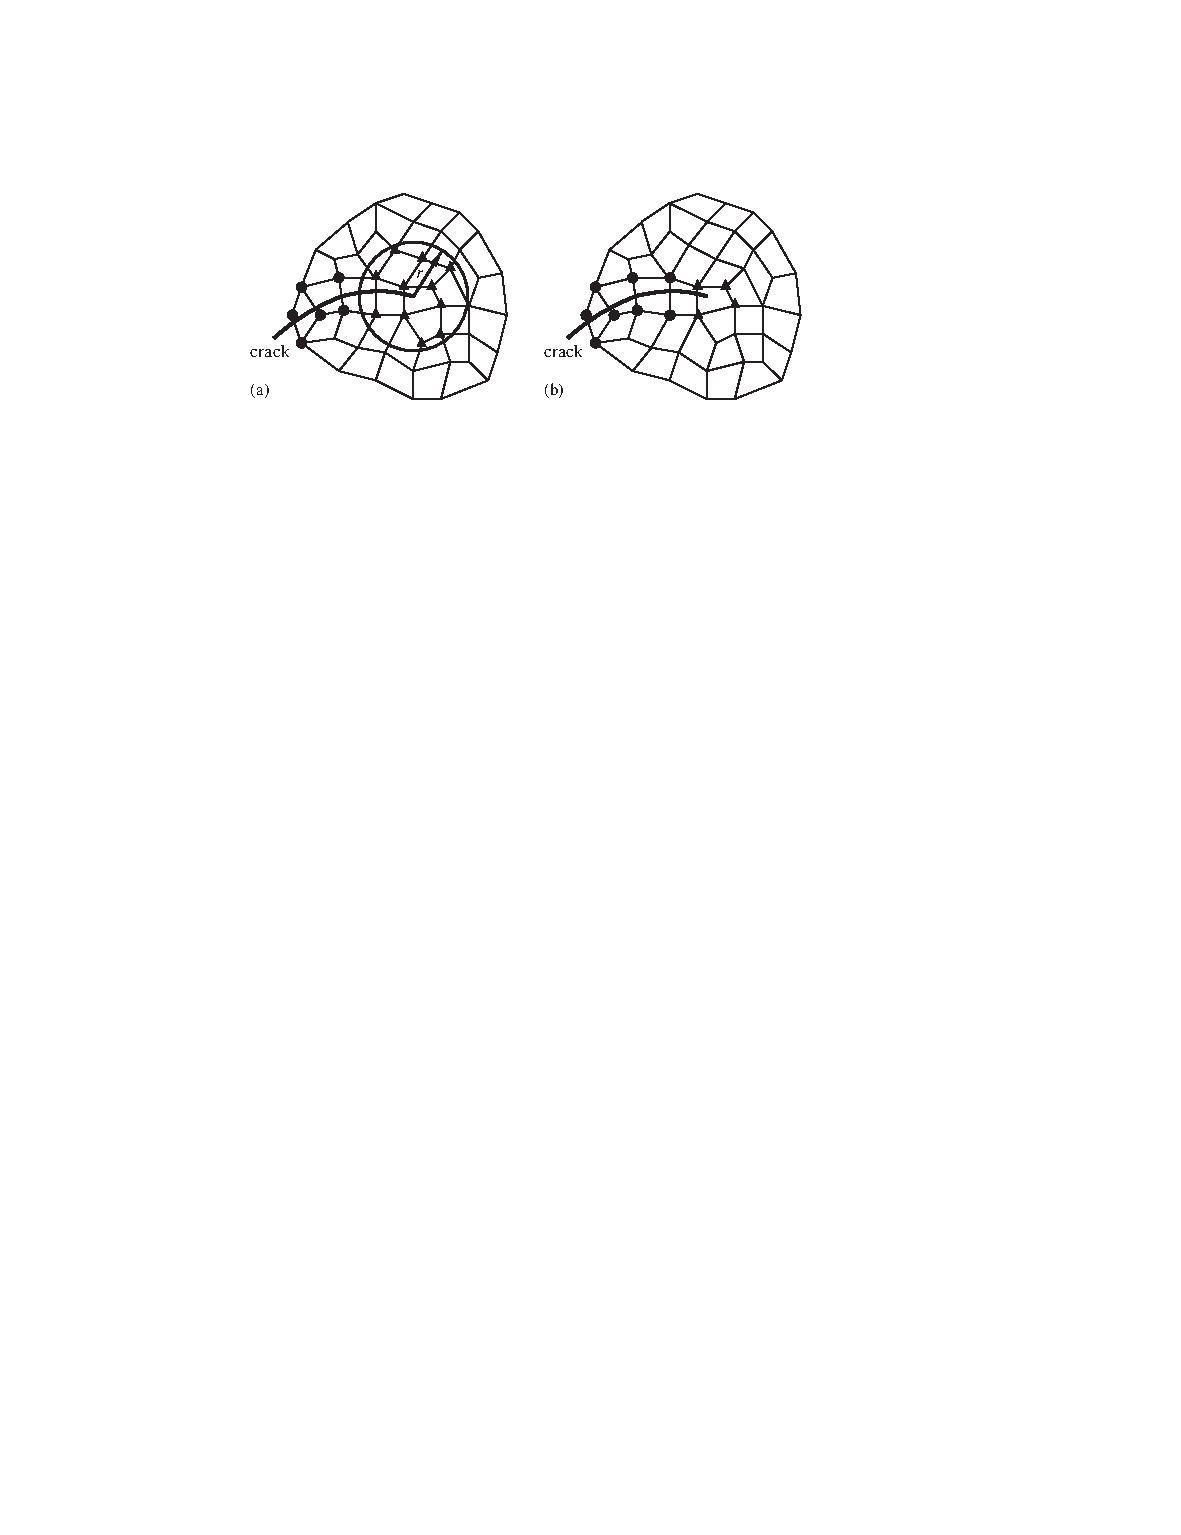
\includegraphics{XFEMenrichments}
\caption[XFEM models enrich nodes around a discontinuity]{XFEM models enrich nodes around a discontinuity\cite{fries2010extended}}
\label{fig:XFEM}
\end{figure}
%

More recently, Sauerland and Fries applied XFEM to two phase flow problems \cite{sauerland2013stable}, including standard dam-breaking and rising droplet problems.
Holl et al.~\cite{holl2013adaptive} used XFEM in the multi scale modeling of crack propagation, including multiple interacting cracks.
Mohammadnejad and Khoei~\cite{mohammadnejad2013hydro} and Hunsweck et al. \cite{hunsweck2013finite} modeled using XFEM the combination of fluid and fracture behavior found in hydraulic fracturing, a topic of considerable recent interest.

A second common method of modeling material failure is the Reproducing Kernel Particle Method (RKPM), developed by Liu et al.~\cite{liu1995reproducing}.
Mesh-based models track the connections between points in a deforming material, which can become problematic when large deformations deform the mesh and even cause it to intersect itself.
RKPM is a ``mesh free'' method that tracks material properties by their values at selected points.
Mesh-free methods are advantageous for modeling large deformation in fluids and solids because they do not track connections between points.
Between material points, properties are interpolated from their values at nearby points by way of integration with a kernel function.
The difference in domains between RKPM and XFEM can be seen in \cref{fig:FEMvsRKPM}.
%
\begin{figure}[h]
  \centering
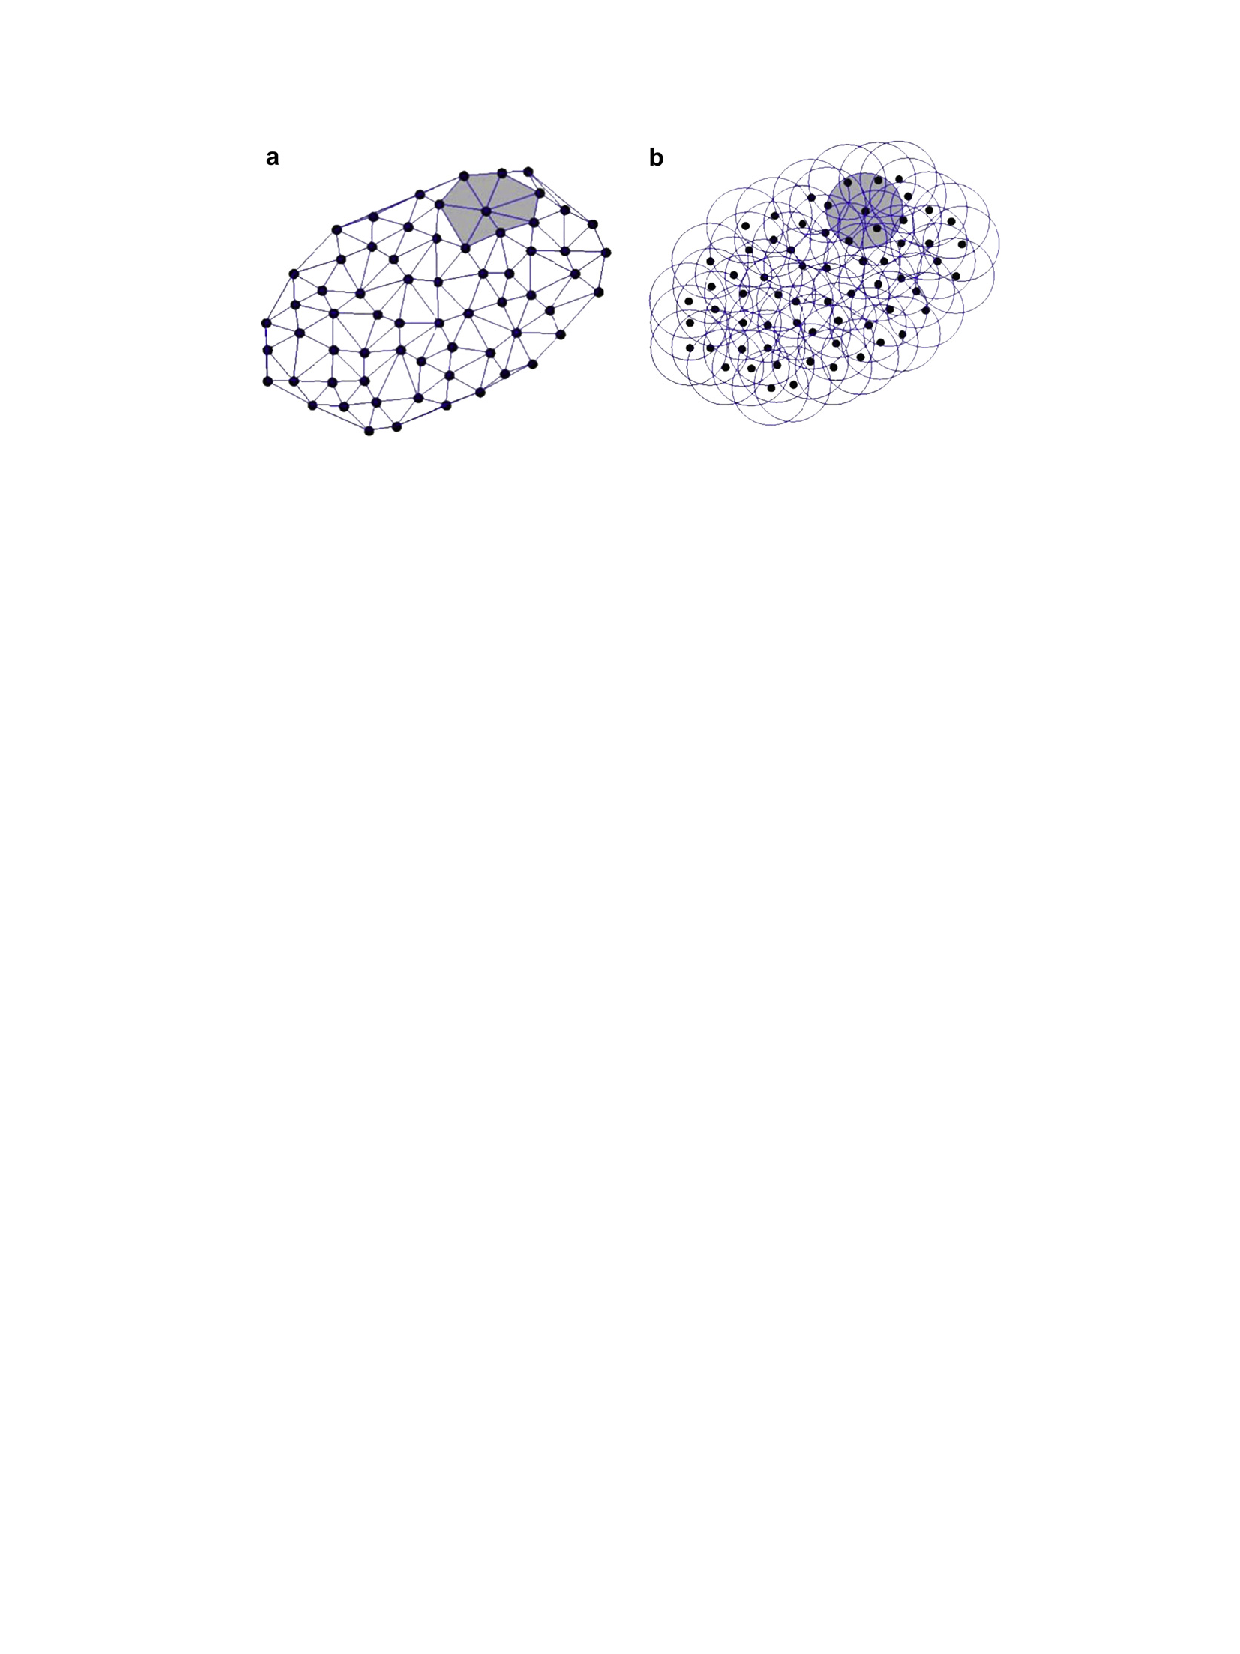
\includegraphics{FEMvsRKPM}
\caption[Comparison of domains of influence for FEM and RKPM]{Comparison of domains of influence for a)FEM and b)RKPM, by Guan et al. \cite{guan2011semi}}
\label{fig:FEMvsRKPM}
\end{figure}
%
The key to the RKPM lies in this kernel function; by using window functions from wavelet analysis, a ``reproducing'' kernel guarantees that  integrals of interpolated properties reproduce the integral of the continuous property field.
The ``reproducing'' kernel makes the RKPM a Partition of Unity method like XFEM, and is a major advantage of RKPM relative to other particle methods.
It is, however, computationally expensive.

In its original formulation, the RKPM successfully handles large deformations that would cause unacceptable distortion in Finite Element models.
A semi-Lagrangian version implemented by Guan et al. in \cite{guan2009semi} allows for recalculation of the support function.
This allows damage in the form of severing the relationship between points that have been pulled too far apart.
Recent applications of the RKPM include the work of Guan et al. on fragment-impact problems~\cite{guan2011semi} and analysis of non-linear wave equations by Cheng and Kim Meow~\cite{cheng2012analyzing}.
The RKPM has also been used by Xie and Wang~\cite{xie2014stabilized} to analyze coupled hydro-mechanical behavior.
Wu et al. have coupled RKPM and FEM in their recent work on fragmentation and debris evolution\cite{wu2014fragmentation}.

Other methods of modeling failure include multiple finite element techniques and particle methods.
Finite element methods incorporating ``element death'' remove from consideration elements that meet particular criteria and are perhaps the simplest way of modeling material failure.

Cohesive zone elements, proposed by Ortiz et al.~\cite{ortiz1987finite}, use element level information to detect the onset of plasticity (material instability) and add suitable deformation modes to model shear banding.
The additional deformation modes allow cohesive zone elements to capture the more complex displacements associated with plastic shear bands.
Other cohesive zone elements developed by Needleman\cite{needleman1987continuum} model crack growth, but Foulk et al.\cite{foulk2000formulation} note that this requires very fine meshes or prior knowledge of the crack path.
They are useful for cases such as composite delamination or debonding, where the crack follows a known surface.
Fang et al. propose in \cite{fang2011augmented} a method of augmenting the cohesive zone model to work in concert with XFEM-type elements to model both arbitrary and known crack paths.
More recently, McGarry et al. \cite{mcgarry2014potential} and M\'airt\'in et al. \cite{mairtin2014potential} developed a cohesive zone model to account for crack closure, including crack surface tractions.

Particle methods of modeling failure include the Smooth Particle Hydrodynamic (SPH) method, reviewed by Monaghan in \cite{monaghan2005smoothed}, in which a kernel (commonly a cubic spline) is used to create a smooth interpolation of actual quantities.
Developed for fluids, Springel notes in \cite{springel2010smoothed} that it is often used in astrophysics problems, where many fluid problems are encountered and even ``solid" bodies deform under their own gravity.
It can also predict elastic behavior and has been extended with failure models by Benz and Asphaug in \cite{benz1995simulations} by adding an evolving damage parameter.
Particle methods like SPH handle fragmentation very well, and are used in a variety of problems with material interfaces, high strains, and multiphase and multi-physics aspects.
Because cubic spline kernels do not reproduce a Partition of Unity, property interpolation does not accurately reproduce the continuum field.
Additionally, elastic SPH models do not conserve angular momentum, and in cases require artificial viscosities or artificial stresses to avoid numerical instability.

The Material Point Method, developed by Sulsky and Schreyer in~\cite{sulsky1996axisymmetric}, tracks points in both Eulerian and Lagrangian meshes.
The advantage of using both meshes is an ability to handle obstacles and boundary conditions without difficulty at large deformations.
Wieckowski notes that the downside to using both meshes is continual remeshing and added computational expense \cite{wikeckowski2004material}.
Despite this expense, the material point method was extended to model cracks by Nairn in \cite{nairn2003material}, then further enhanced by Sadeghirad et al. in \cite{sadeghirad2011convected} to improve stability when modeling massive deformations.
The Lattice Discrete Particle Method was developed by Cusatis et al.\cite{cusatis2011lattice,cusatis2011blattice} to model concrete.
It fills a volume with variously-sized particles generated from a probability density function based on aggregate size.
The relationships between these particles form tetrahedrons (the lattice) that fill the volume and allow multi-particle interaction.
Failure occurs at predefined surfaces between particles and can include various failure modes.
The LDPM is capable of accurately modeling many failure conditions in concrete, including the impact of specimen size on effective material behavior.
These are only a few of the myriad of models that attempt to model the progression of material failure.

All of these methods are used to solve a partial differential equation for conservation of momentum in a continuum. 
Because they are based on continuum PDEs, they do not naturally develop discontinuous displacements such as cracks. 
The PDEs that govern these methods are ill-defined at the surface of a crack, so cracks must be inserted within or between elements after discretization. 
This results in crack propagation that is discretization-dependent as well as computationally expensive and potentially unstable. 
Although progress in addressing these issues continues, much of the difficulty is essentially tied to the undefined nature of derivative equations at discontinuous displacements.
By abandoning the use of displacement derivatives, peridynamics offers an alternative way to address discontinuous displacements.
%

\section{Peridynamic Modeling}
The term \textit{peridynamic} was coined by Silling to describe the new formulation of continuum mechanics he developed in \cite{silling2000reformulation}.
From the Greek roots \textit{peri} and \textit{dyna} meaning \textit{near} and \textit{force} respectively, it alludes to the nonlocal force exerted by nearby points.
In contrast to the nonlocal continuum mechanics models of Kr\"oner, Eringen and Edelen \cite{kroner1967elasticity,eringen1972nonlocal,eringen1983differential}, the peridynamic model casts material behavior at a point as an \textit{integral} equation of the surrounding displacement rather than the classical \textit{differential} equation.
Because peridynamic models do not include spatial displacement derivatives, discontinuous displacements can arise naturally and can be analyzed without special heuristics. 
In classical continuum mechanics, linear momentum is conserved according to the local  \cref{eq:ClassicCoPV},
%
\begin{equation}
\label{eq:ClassicCoPV}
\rho(\mathbf{x})\ddot{\mathbf{u}}(\mathbf{x}) = \nabla \cdot \mathbf{P}(\mathbf{x}) + \mathbf{b}(\mathbf{x})
\end{equation}
%
in which $\rho$ is the density, $\ddot{\mathbf{u}}$ is the second time derivative of displacement , $\mathbf{P}$ is the transpose of the First Piola Kirchhoff stress tensor, and $\mathbf{b}$ is the body force density, all of which are functions of position $\mathbf{x}$ and of time. 
Because \(\mathbf{P}\) is defined in terms of the deformation gradient, it is clear that \cref{eq:ClassicCoPV} is undefined for discontinuous displacements. 
In fact, traditional models require even the first spatial derivative of displacement to be continuous.
Strongly nonlocal models (including peridynamics) replace the divergence-of-stress term with an integral functional,
%
\begin{equation}
\label{eq:PDCoPV}
\rho(\mathbf{x})\ddot{\mathbf{u}}(\mathbf{x}) = \int_\Omega \mathbf{f}(\mathbf{x},\mathbf{q}) dV_\mathbf{q}  + \mathbf{b},(\mathbf{x})
\end{equation}
%
so that, instead of the divergence of stress, we have the integral of a ``force" function $\mathbf{f}$ of the position vector $\mathbf{x}$ and the position vector $\mathbf{q}$ of a point within the body domain $\Omega$. 
This force function may depend on \(\mathbf{x}\), \(\mathbf{q}\), their deformed positions, the original and deformed positions of other points in \(\Omega\), history, etc.
It is common for \(\mathbf{f}\) to be defined as \(0\) for any pair of points initially further than \(\delta\) apart. 
The points within \(\delta\) of a point \(\mathbf{x}\) are the \textit{neighborhood} of \(\mathbf{x}\) and are denoted in \cref{fig:PDbody} by \(\mathcal{H}\).
%
\begin{figure}[h]
  \centering
\subinputfrom{\diagrampath}{PDbody.eps_tex}
\caption{A peridynamic body \protect\(\Omega\protect\)}
\label{fig:PDbody}
\end{figure}
% 
By including the behavior of nearby material, these models introduce an inherent length scale to the model. 
This length scale may be determined by material properties or by computational demands.

Constitutive modeling of a wide variety of materials is accomplished by choosing the appropriate form for the force function.
While the simplest force functions recreate a one-parameter linear elastic solid material, other force functions can be used to model a wide variety of material behaviors, some of which will be outlined here.
Most simulation of material behavior uses an equation of motion reformulated for a discretized model.
When discretized, peridynamics is typically a mesh-free numerical method in which there are no geometrical connectivities between various nodes.

A force function can be restricted to being pairwise (depending solely on the displacement of the two points \(\mathbf{x}\) and \(\mathbf{q}\)), and still model complex and varied behavior.
By including a damage parameter that sets the force contribution of ``damaged'' bonds to \(0\), Silling and Askari\cite{silling2005meshfree} were able to model a brittle material with natural crack formation, propagation, and branching.
Other examples of damage propagation include impacts against brittle structures as in \cref{fig:PDimpact} modeled by Demmie and Silling\cite{demmie2007approach} and fracturing of thermally-stressed glass modeled by Kilic and Madenci\cite{kilic2009prediction}. 
%
\begin{figure}[h]
  \centering
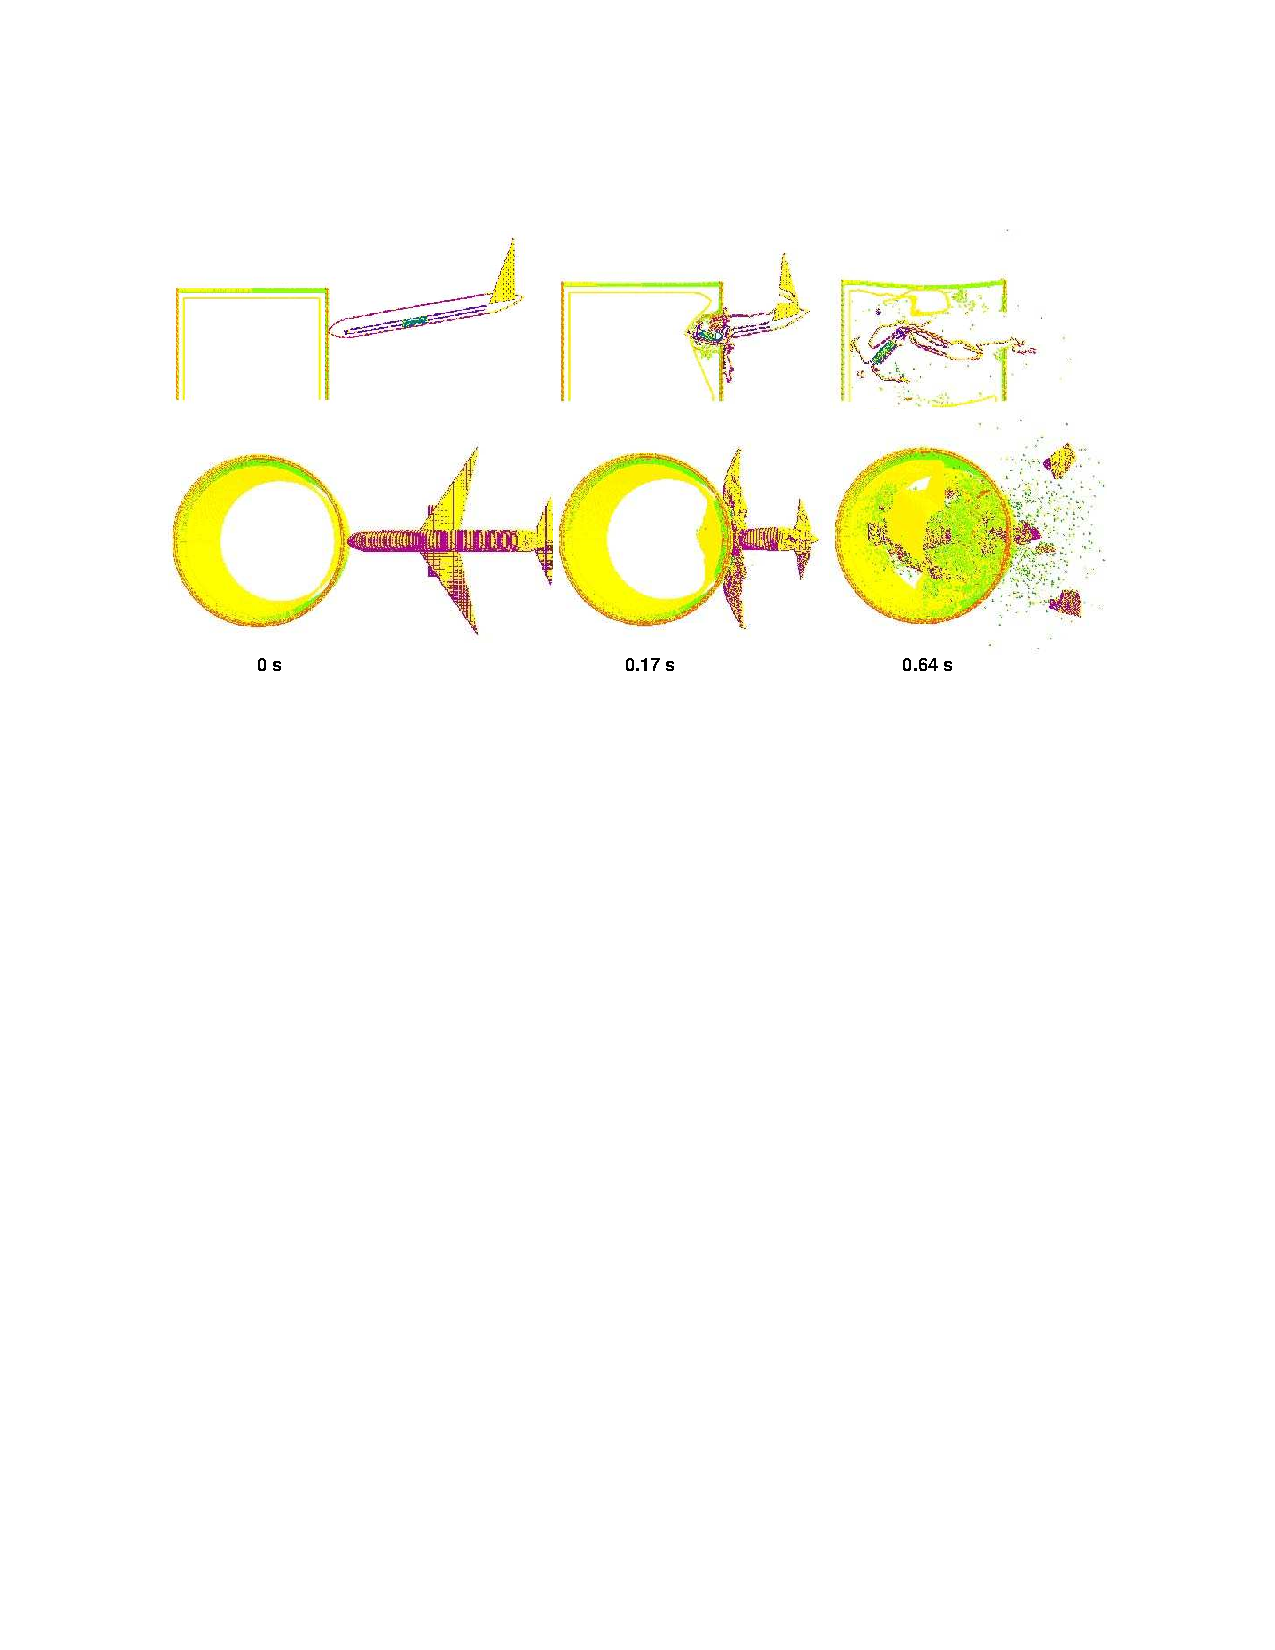
\includegraphics[width=0.8 \textwidth]{demmie07impact}
\caption[Peridynamic model of an airplane impacting a concrete structure]{Peridynamic model of an airplane impacting a concrete structure \cite{demmie2007approach} }
\label{fig:PDimpact}
\end{figure}
%
Modeling progressive fracture, including crack branching, is a major advantage of peridynamic formulations.
Using a piecewise force function, Dayal and Bhattacharya~\cite{dayal2006kinetics} were able to model phase transformation in 1D and 2D without an additional constitutive law; the transformations arose and propagated naturally as a dynamic instability, a result of the force function used.
Peridynamic models have also been used to analyze composite laminates.
In \cite{xu2008peridynamic}, Xu et al. designate peridynamic bonds as fiber or matrix bonds with different force functions to model damage in composite laminates. 
Kilic et al. model fiber, matrix, and interfacial bonds in \cite{kilic2009peridynamic} to capture stacking order effects on damage propagation.
Bobaru~\cite{bobaru2007influence} applied the peridynamic model to nano fiber networks, at a scale where long-range forces are very apparent.
In the same paper he created a Representative Volume Element (RVE) for random networks of nano fibers, laying the ground work for peridynamic multi-scale modeling.
Also related to multi-scale peridynamic modeling is work by Silling on model coarsening \cite{silling2011coarsening}, \cref{fig:PDmultiscale}.
An example of a multi-scale peridynamic simulation can be found in \cite{askari2008peridynamics}, by Askari et al.
%
\begin{figure}[h]
  \centering
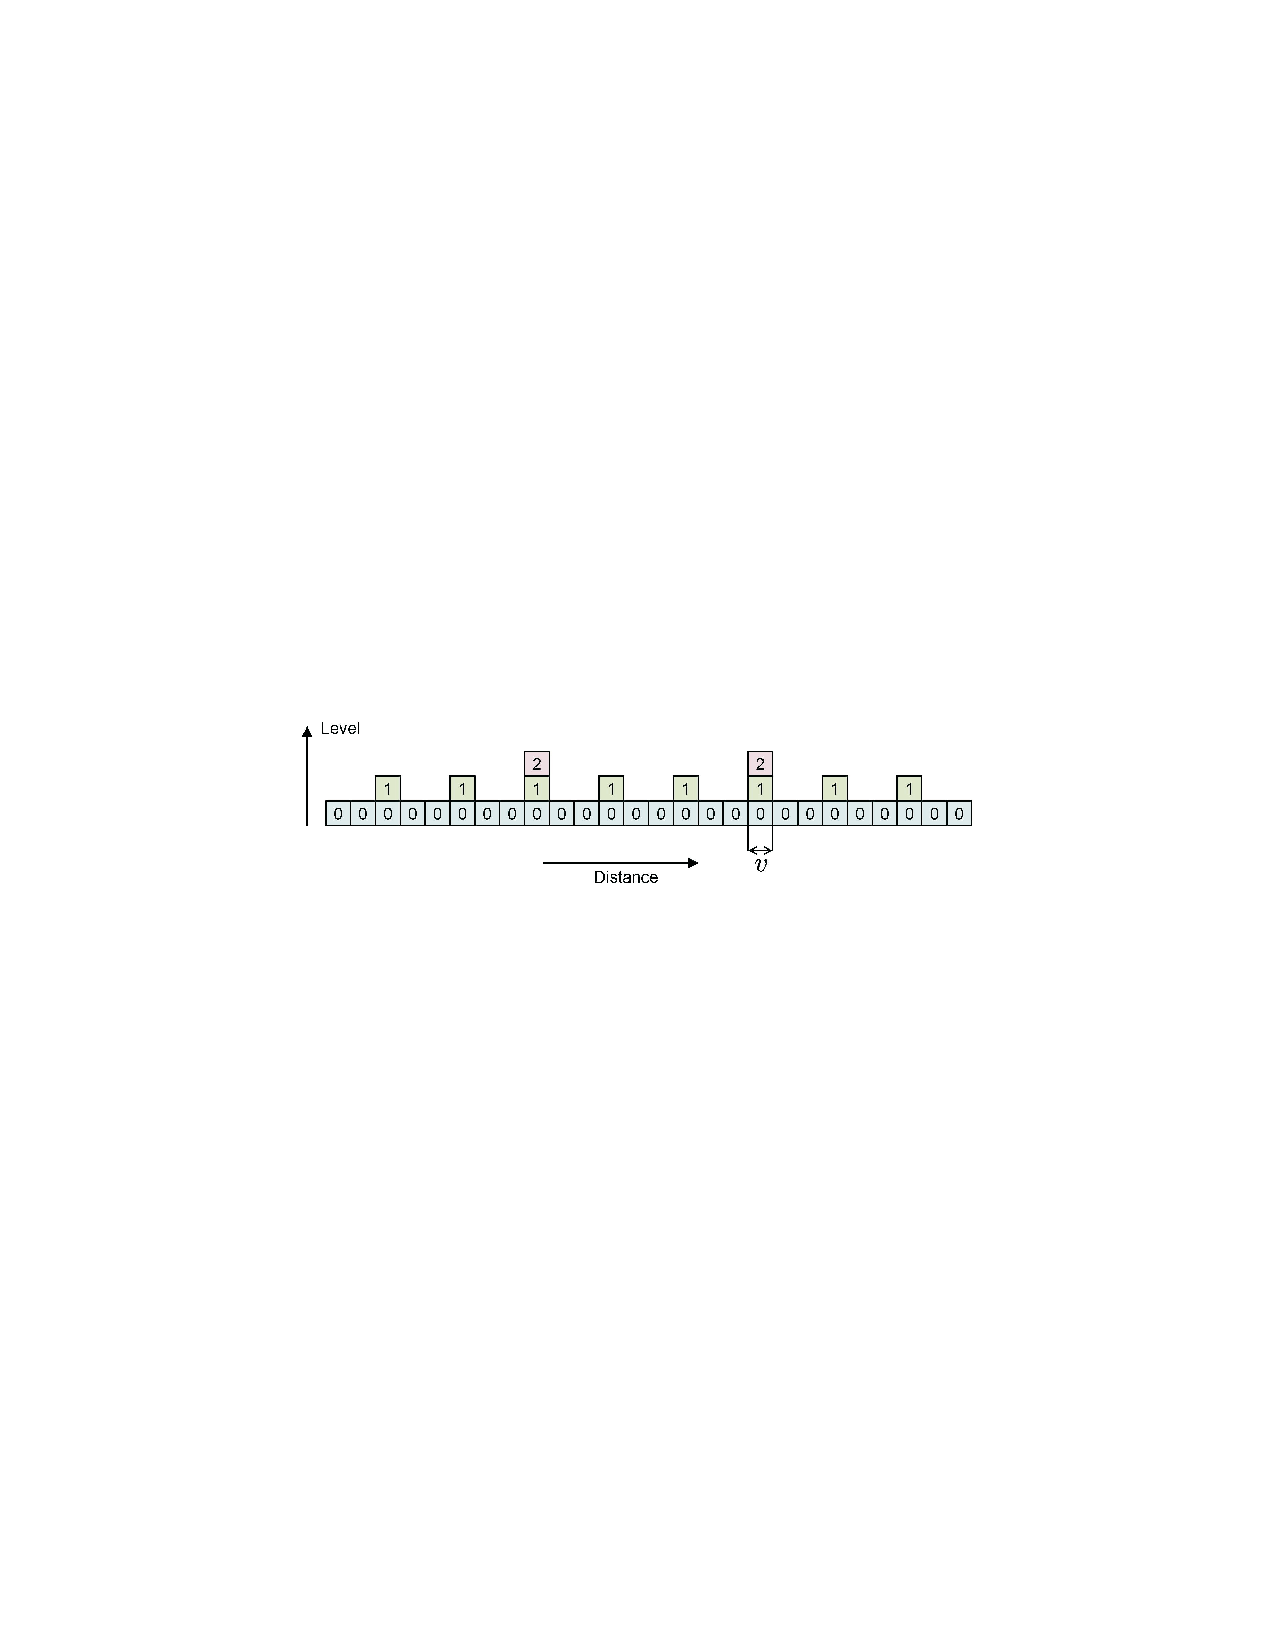
\includegraphics{PDmultiscale}
\caption[Silling's illustration of course-graining in time]{Silling's illustration of course-graining in time from \cite{silling2011coarsening}.}
\label{fig:PDmultiscale}
\end{figure}
%

Concrete is a nearly standard example material in which nonlocal behavior is easily observed, and modeling the damage accumulation and proceeding discontinuity propagation has long been the goal of nonlocal models developed by Bazant and Pijaudier-Cabot~\cite{bazant1988nonlocal} among others, significantly predating peridynamics.
In \cite{gerstle2007peridynamic}, Gerstle et al. use rotational degrees of freedom to create a concrete material model, capable of describing a linear elastic material with any Poisson ratio, that also handles material failure.
Peridynamic models are not limited to force-displacement relationships; the theory has also been applied to diffusion processes and multiphysics problems.
Peridynamic models can simulate heat transfer~\cite{bobaru2010peridynamic} and diffusion~\cite{burch2011classical}.

Mathematical analyses of simplified cases have also been fruitful.
Weckner~\cite{weckner2005effect} determined analytical solutions to the infinite bar problem. 
Emmerlick and Zimmerman proved solution existence and uniqueness in the simplest case of the peridynamic bar~\cite{emmrich2007analysis}.
Mikata found additional analytical solutions for the bar problem~\cite{mikata2012analytical}.
In 3D, Weckner constructed Green's functions for an infinite peridynamic solid in \cite{weckner2009green}.
All of this work was done with peridynamic models limited to pairwise force functions.

Other than Gerstle's aforementioned micropolar peridynamic model, the pairwise force function limits 3D solid materials to a Poisson ratio of  \(\nu=\sfrac{1}{4}\). 
To model additional material behavior, Silling et al. reinvented the underlying peridynamic concept of bonds and forces and introduced state-based peridynamic models in \cite{silling2007peridynamic}.
By freeing the force function from the pairwise restriction, state-based models allow the force relationship between two points to depend on the collective behavior of all nearby material.
Using the concept of a deformation vector state allows for the construction of correspondence models that can recreate any classical constitutive model.
These correspondence models use the deformation state to approximate the deformation gradient tensor, then use the deformation gradient tensor to calculate force contributions.
State-based models were used by Foster et al. to simulate viscoplasticity and hardening in~\cite{foster2010viscoplasticity}, and rate dependent failure in~\cite{foster2011energy}, with others, via an energy criterion.
Mitchell describes state-based models for plasticity in~\cite{mitchell2011nonlocal} and viscoelasticity in~\cite{mitchell2011non}.
A non-ordinary state-based model was used by Warren et al. to simulate fracture in~\cite{warren2009non}.
More recently, Tupek et al. have incorporated the idea of peridynamic damage into a Johnson-Cook based damage state that accumulates with plastic strain\cite{tupek2013approach}.
%
\section{Other Nonlocal Elasticity Models}
\label{sec:NLbeams}
%
The peridynamic formulation of continuum mechanics is neither the only nor the first nonlocal model. Nonlocal elasticity generally allows for forces at a point that are dependent on the material configuration of an entire body, rather than the configuration at that point \cite{eringen1972nonlocal}.  While long-range forces are obvious at the molecular model, material at larger scales is conventionally modeled as though internal forces are local or contact forces \cite{kroner1967elasticity}.
The result of such approximation is accurate for deformations that are homogeneous, but introduces some inaccuracy for inhomogeneous deformations like the propagation of waves with short wavelengths.
One way to distinguish between homogeneous and inhomogeneous deformations is to incorporate higher-order gradients of deformation.
While stress in classical elasticity is a function of the (first) gradient of deformation, Eringen's formulation of a nonlocal modulus in \cite{eringen1983differential} approximates a weighted sum of the first and second order gradients.
This introduces a length scale to the model and has the effect of smearing out local deformation inhomogeneities over the surrounding material, while maintaining the conventional result for homogeneous deformations.

Previous work in the nonlocal mechanics of beams is motivated by the observed stiffening of nanoscale cantilevers.
Challamel and Wang demonstrate in \cite{Challamel2008small} that Eringen nonlocal elasticity cannot reproduce the scale stiffening, but that stiffening does result from other gradient-elastic models and models incorporating nonlocal curvature.
Because all of these models incorporate higher-order gradients of deformation, they impose stronger continuity requirements than classical elasticity, and are unsuitable for discontinuous displacements.
Because the gradients are evaluated locally, gradient models are called \textit{weakly nonlocal}.
Recent work by Paolo et al. \cite{paola2013mechanically} develops a displacement-based beam in which relative axial displacement, shear displacement, and rotation of non-adjacent beam segments are resisted by three kinds of nonlocal spring, whose stiffnesses can be tuned to the expected material behavior.
With the appropriate nonlocal stiffnesses, their model reproduces the nanoscale cantilever stiffening effect.

Similarly, Duan and Wang \cite{duan2007exact} applied Eringen-type elasticity to the quasi-1D problem of axisymmetric bending in nanoscale plates.
Pradhan and Murmu~\cite{pradhan2009small} extended the concept to buckling in single-layered graphed sheets, a fully 2D problem.
Later, Ansari et al.~\cite{ansari2010nonlocal} modeled the vibration of single-layered graphed sheets using Eringen-type elasticity.

Nonlocal effects have also been incorporated into many of the modeling techniques previously discussed.
Bazant and Chang incorporated nonlocal strain-softening into a finite element model in \cite{bazant1987nonlocal}.
Any interpolating particle method will exhibit some measure of nonlocality, but some explicitly model nonlocal phenomena.
Vignjevic et al. used SPH to model nonlocal strain-softening in \cite{vignjevic2014sph}, and in \cite{burghardt2012nonlocal}, Burghardt et al. developed a material point method that incorporates nonlocal plasticity.

\section{Thin Features}
Many engineering analyses concern shapes that have one dimension much greater than another; numerical modeling the behavior of these shapes can be a considerable challenge for methods designed for 3D solids. 
In finite element models, for example, calculations can become unstable or too stiff when individual elements become long and thin. 
To avoid such elements while maintaining model fidelity requires a very large number of solid elements. 
By making some assumptions about the behavior along the thin direction, many such shapes can be modeled as 1D beams or 2D plates or shells without great loss of accuracy.
A comprehensive review of the classical continuum mechanics associated with thin features by Reddy \cite{reddy2007theory} also includes a section on the Finite Element analysis of plates and shells.
Material failure in classical thin features is modeled using the same techniques as in solids.
Dolbow et al. use XFEM in~\cite{dolbow2000modeling} to model fracture in plates.
Li et al. use a variant of RKPM in~\cite{li2000numerical} to model plastic deformation in shells.
More recently, Xu et al. have applied XFEM to plate plasticity problems\cite{xu2013xfem}, and Memar Ardestani et al. have used RKPM to model functionally graded plates\cite{memar2014analysis}.
Other authors use cohesive zone elements\cite{li2002analysis} or SPH\cite{maurel2008sph} to study failure in thin features.
%

\subsection{Peridynamic Models}
Reduced dimension thin features such as bars\cite{silling2003deformation,weckner2005effect,emmrich2007analysis,mikata2012analytical}, plates\cite{kilic2009prediction}, and membranes\cite{silling2005peridynamic} have been modeled using peridynamics, but these models are used for in-plane or membrane forces as shown in \cref{fig:PDmembrane}.
%
\begin{figure}[h]
  \centering
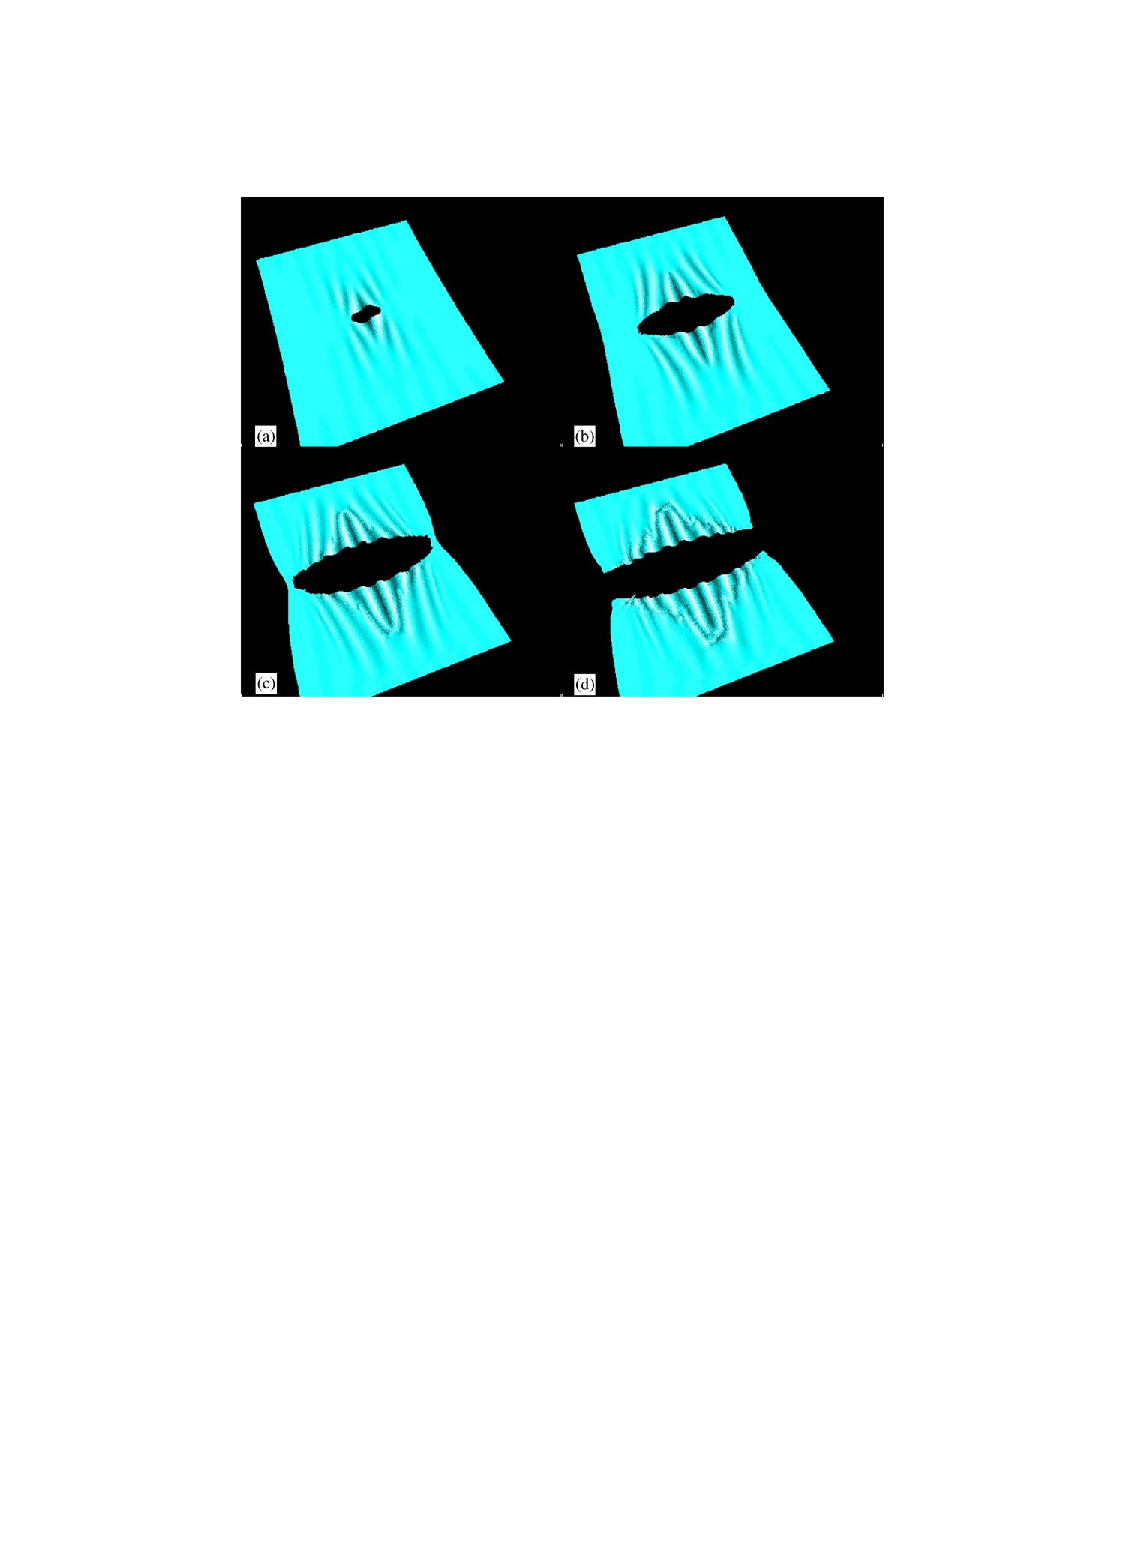
\includegraphics{PDmembrane}
\caption[Tearing a peridynamic membrane]{Tearing a peridynamic membrane \cite{silling2005peridynamic}}
\label{fig:PDmembrane}
\end{figure}
%
Because traditional peridynamic models exert forces in the direction of the bonds between points, they are not well-suited for bending problems of thin shapes, in which force and displacement are both nearly perpendicular to bonds connecting material points at separate points on a surface.
Just as with solid finite elements, most peridynamic models of thin features like the tubes in \cref{fig:LittlewoodCylinder} have included several nodes through the thickness of a thin part to capture bending behavior.
Also as with solid finite elements, this leads to very fine discretization of thin features, even when the expected behavior is quite simple.
This greatly increases the computational expense of modeling parts with thin features.
%
\begin{figure}[h!]
  \centering
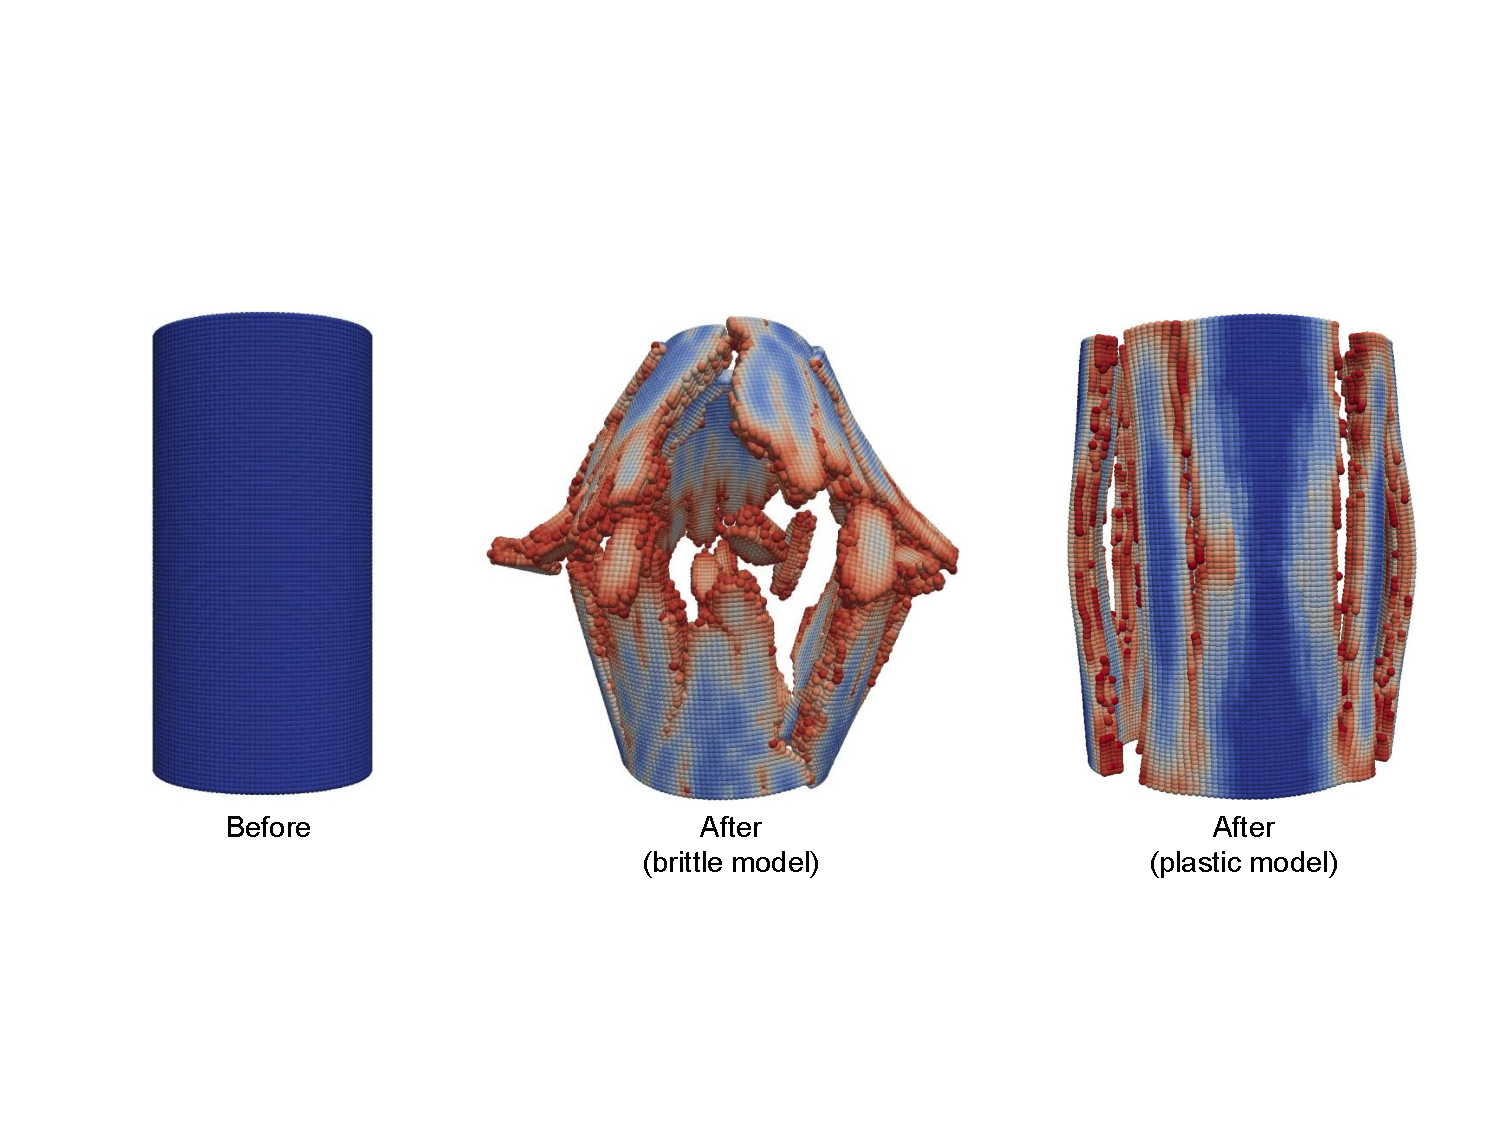
\includegraphics[width=0.9 \textwidth]{LittlewoodCylinder}
\caption[A peridynamic cylinder uses several nodes through its thickness]{A peridynamic cylinder uses several nodes through its thickness in \cite{littlewood2010simulation}}
\label{fig:LittlewoodCylinder}
\end{figure}
%

A recent paper by Taylor and Steigmann~\cite{taylor2013two} partially addresses this issue by starting with mathematical analysis of the continuous 3D bond-based peridynamic solid model of a thin plate.
By using a continuous model, they avoid the difficulties associated with discretizing thin features.
Applying asymptotic analysis to the continuous model, they reduce a 3D solid model to 2 dimensions.
The asymptotic reduction is accomplished by the addition of degrees of freedom for the derivative of displacement with respect to the through thickness direction.
By making the through-thickness derivative of displacement vector an independent variable, the resulting flat model includes a measure of angular deformation that allows resistance to bending.
Using a simple bond-stretch damage criterion, the Taylor and Steigmann's reduced model was able to capture the out-of-plane displacement (\cref{fig:TaylorTransverse}) associated with crack propagation behavior (\cref{fig:TaylorCrack}) in a pre-cracked plate under tension loading.
In general, however, the asymptotic reduction model encounters difficulty when nonlinear behaviors like damage are implemented.
The use of a bond-stretch criterion as implemented is only appropriate when deformation is dominated by in-plane tension, as failure caused by bending will not be captured.
Because of its basis in the 3D bond-based solid model, Taylor and Steigmann's model is limited to a Poisson's ratio of \sfrac{1}{3}.
While it is possible that future analysis will extend the asymptotic reduction to state-based model, allowing for arbitrary Poisson's ratios, there are significant mathematical hurdles that will have to be overcome.

%
\begin{figure}[h!]
  \centering
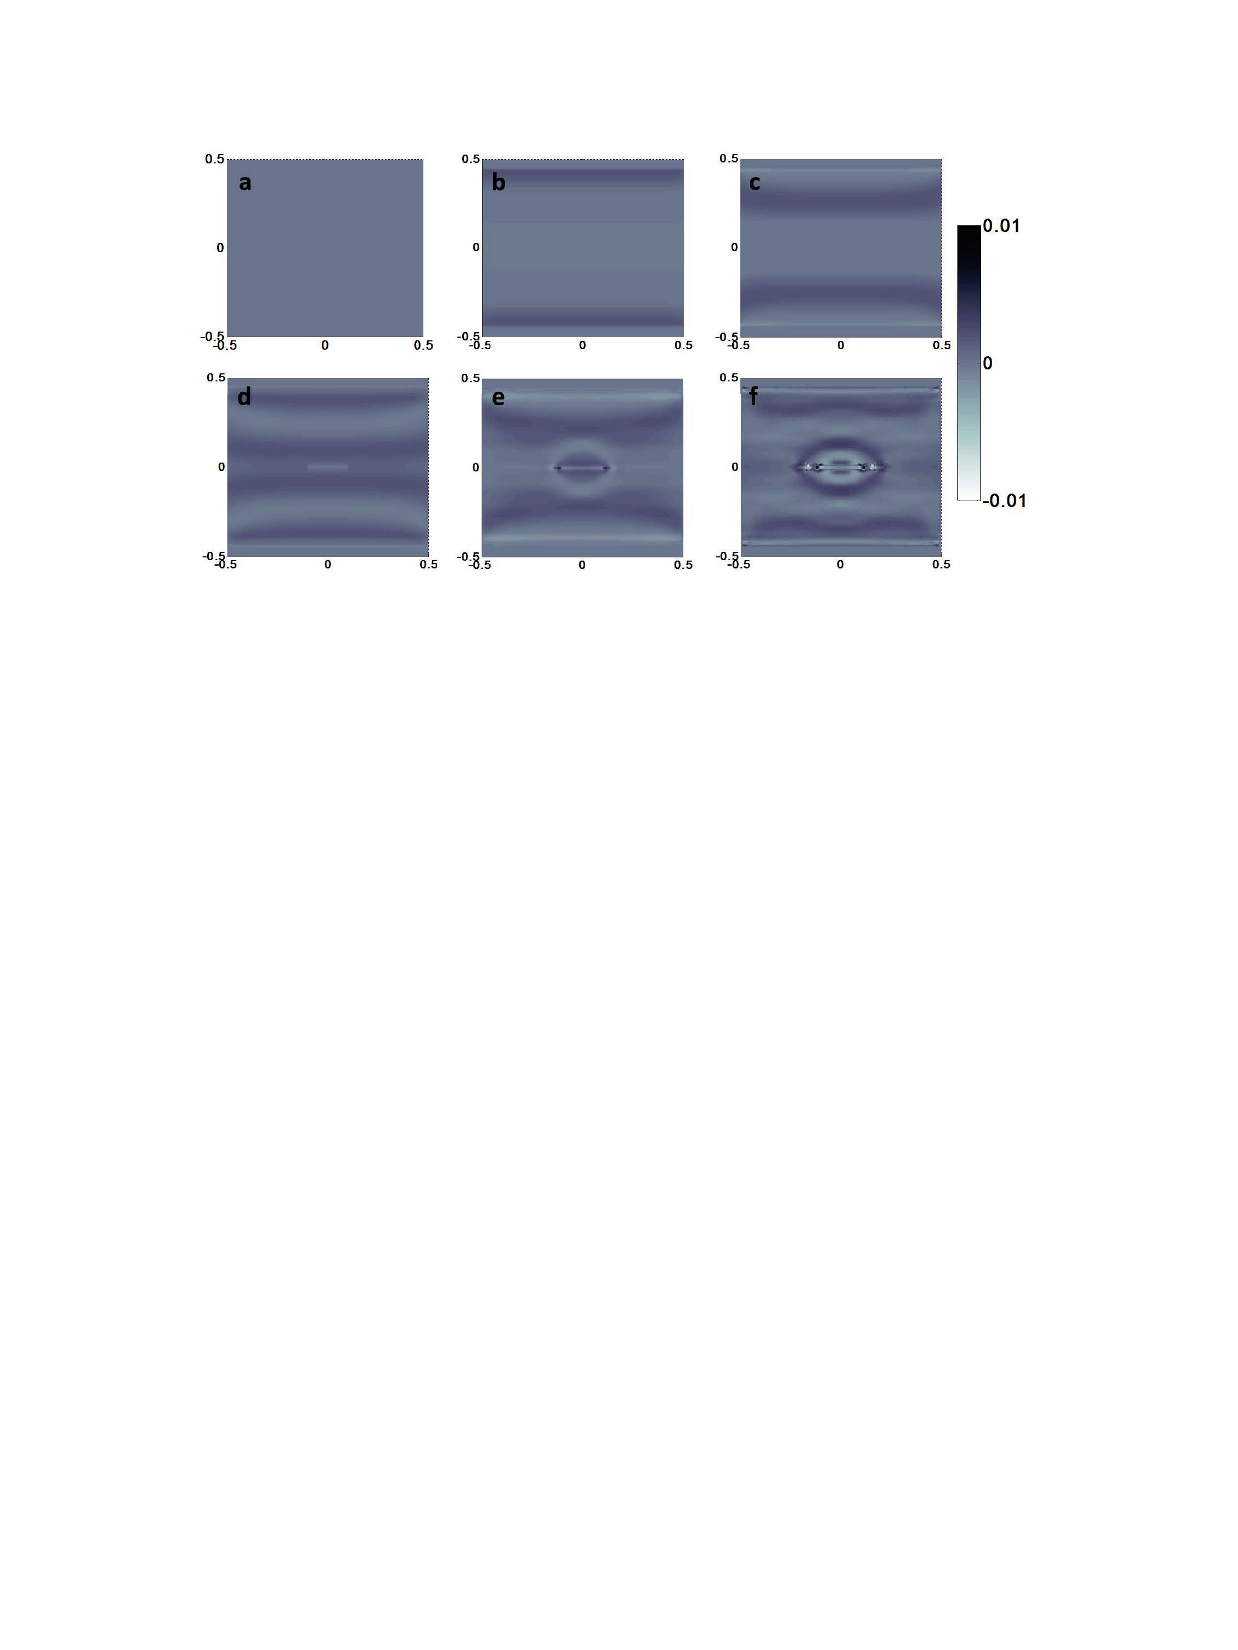
\includegraphics[width=0.9 \textwidth]{TaylorTransverseDisp}
\caption[Taylor and Steigmann plate transverse displacement]{Taylor and Steigmann's asymptotic reduction allows for bending resistance in a 2D plate in tension~\cite{taylor2013two}}
\label{fig:TaylorTransverse}
\end{figure}
%
%
\begin{figure}[h!]
  \centering
\includegraphics[width=0.4 \textwidth]{Taylor2DCrack}
\caption[Taylor and Steigmann plate cracking]{Taylor and Steigmann's crack propagation for \cref{fig:TaylorTransverse} plot \textbf{f}~\cite{taylor2013two}}
\label{fig:TaylorCrack}
\end{figure}
%

A nonordinary model similar to those proposed by Silling in \cite{silling2007peridynamic} and \cite{silling2010peridynamic} allows for a simple bending model that can be used for one- and two-dimensional models.

%Recent work by Oterkus includes additional degrees of freedom to describe the orientation of each peridynamic point, so that each bond between points has components for differential displacements and for differential orientations. 
%These are incorporated into a bond-based thin feature model for beams, plates and shells. 
%These models appear to include spatial derivatives and in the case of plates are constrained to the same Poisson ratio as other bond-based models.
